%%%%%%%%%%%%%%%%%%%%%%%%%%%%%%%%%%%%%%%%%%%%%%%%%%%%%%%%%%%
 \chapter{Systems of Linear Equations}\label{chap:1}
	\input{1-systems-of-linear-equations/1-solutions-and-elementary-operations}
        \section{Gaussian Elimination}
\label{sec:1_2}

\index{gaussian elimination!systems of linear equations and}\index{system of linear equations!gaussian elimination}
The algebraic method\index{algebraic method}\index{solution!algebraic method} introduced in the preceding section can be summarized as follows: Given a system of linear equations, use a sequence of elementary row operations to carry the augmented matrix to a ``nice'' matrix (meaning that the corresponding equations are easy to solve). In Example \ref{exa:000809}, this nice matrix took the form
\begin{equation*}
\leftB \begin{array}{rrr|r}
	1 & 0 & 0 & * \\
	0 & 1 & 0 & * \\
	0 & 0 & 1 & *
\end{array} \rightB
\end{equation*}
The following definitions identify the nice matrices that arise in this process.

\newpage
\begin{definition}{Row-Echelon Form (Reduced)}{000992}
A matrix is said to be in \index{row-echelon form}\textbf{row-echelon form} (and will be called a \index{row-echelon matrix}\index{matrix form!row-echelon form}\index{matrix!row-echelon matrix}\textbf{row-echelon matrix}) if it satisfies the following three conditions:

\begin{enumerate}
\item All \index{zero rows}\index{rows!zero rows}\textbf{zero rows} (consisting entirely of zeros) are at the bottom.

\item The first nonzero entry from the left in each nonzero row is a $1$, called the \textbf{leading 1}\index{leading $1$}\index{rows!leading $1$} for that row.

\item Each leading $1$ is to the right of all leading $1$s in the rows above it.

\end{enumerate}

A row-echelon matrix is said to be in \index{reduced row-echelon form}\textbf{reduced row-echelon form} (and will be called a \index{reduced row-echelon matrix}\index{matrix!reduced row-echelon matrix}\index{matrix form!reduced row-echelon form}\textbf{reduced row-echelon matrix}) if, in addition, it satisfies the following condition:

\begin{enumerate}
\setcounter{enumi}{3}
\item Each leading $1$ is the only nonzero entry in its column.

\end{enumerate}
\end{definition}

\noindent The row-echelon matrices have a ``staircase'' form\index{staircase form}, as indicated by the following example (the asterisks indicate arbitrary numbers).
\begin{equation*}
\leftB \begin{array}{rrrrrrr}
	\multicolumn{1}{r|}{0} & 1 & * & * & * & * & * \\ 
	\cline{2-3}
	0 & 0 & \multicolumn{1}{r|}{0} & 1 & * & * & * \\
	\cline{4-4}
	0 & 0 & 0 & \multicolumn{1}{r|}{0} & 1 & * & * \\
	\cline{5-6}
	0 & 0 & 0 & 0 & 0 & \multicolumn{1}{r|}{0} & 1 \\
	\cline{7-7}
	0 & 0 & 0 & 0 & 0 & 0 & 0 
\end{array} \rightB
\end{equation*}
The leading $1$s proceed ``down and to the right'' through the matrix. Entries above and to the right of the leading $1$s are arbitrary, but all entries below and to the left of them are zero. Hence, a matrix in row-echelon form is in reduced form if, in addition, the entries directly above each leading $1$ are all zero. Note that a matrix in row-echelon form can, with a few more row operations, be carried to reduced form (use row operations to create zeros above each leading one in succession, beginning from the right).

\begin{example}{}{001009}
The following matrices are in row-echelon form (for any choice of numbers in $*$-positions).
\begin{equation*}
\leftB \begin{array}{rrr}
	1 & * & * \\
	0 & 0 & 1
\end{array} \rightB
\leftB \begin{array}{rrrr}
	0 & 1 & * & * \\
	0 & 0 & 1 & * \\
	0 & 0 & 0 & 0
\end{array} \rightB
\leftB \begin{array}{rrrr}
	1 & * & * & * \\
	0 & 1 & * & * \\
	0 & 0 & 0 & 1 
\end{array} \rightB
\leftB \begin{array}{rrr}
	1 & * & * \\
	0 & 1 & * \\
	0 & 0 & 1
\end{array} \rightB
\end{equation*}
The following, on the other hand, are in reduced row-echelon form.
\begin{equation*}
\leftB \begin{array}{rrr}
	1 & * & 0 \\
	0 & 0 & 1
\end{array} \rightB
\leftB \begin{array}{rrrr}
	0 & 1 & 0 & * \\
	0 & 0 & 1 & * \\
	0 & 0 & 0 & 0
\end{array} \rightB
\leftB \begin{array}{rrrr}
	1 & 0 & * & 0 \\
	0 & 1 & * & 0 \\
	0 & 0 & 0 & 1
\end{array} \rightB
\leftB \begin{array}{rrr}
	1 & 0 & 0 \\
	0 & 1 & 0 \\
	0 & 0 & 1
\end{array} \rightB
\end{equation*}
The choice of the positions for the leading $1$s determines the (reduced) row-echelon form (apart from the numbers in $*$-positions).
\end{example}

The importance of row-echelon matrices comes from the following theorem.\index{matrix!row-echelon matrix}\index{row-echelon matrix}

\begin{theorem}{}{001017}
Every matrix can be brought to (reduced) row-echelon form by a sequence of elementary row operations. \index{matrix form!reduced row-echelon form}\index{matrix form!row-echelon form}\index{reduced row-echelon form}\index{reduced row-echelon matrix}\index{row-echelon form}\index{row-echelon matrix}
\end{theorem}

In fact we can give a step-by-step procedure for actually finding a row-echelon matrix. Observe that while there are many sequences of row operations that will bring a matrix to row-echelon form, the one we use is systematic and is easy to program on a computer. Note that the algorithm deals with matrices in general, possibly with columns of zeros. 

\begin{theorem*}{Gaussian\footnotemark Algorithm\footnotemark}{001021}
%\begin{figure}[H]
%\centering
%\includegraphics{1-systems-of-linear-equations/figures/2-gaussian-elimination/ufg01001}
%\caption{\label{fig:001023}}
%\end{figure}

\begin{itemize}
\item[] Step 1. If the matrix consists entirely of zeros, stop---it is already in row-echelon form.

\item[] Step 2. Otherwise, find the first column from the left containing a nonzero entry (call it $a$), and move the row containing that entry to the top position.
\item[] Step 3. Now multiply the new top row by $1/a$ to create a leading $1$.

\item[] Step 4. By subtracting multiples of that row from rows below it, make each entry below the leading $1$ zero.
\end{itemize}

This completes the first row, and all further row operations are carried out on the remaining rows.

\begin{itemize}
\item[] Step 5. Repeat steps 1--4 on the matrix consisting of the remaining rows.
\end{itemize}
The process stops when either no rows remain at step 5 or the remaining rows consist entirely of zeros. \index{gaussian algorithm}
\end{theorem*}
\addtocounter{footnote}{-1}
\footnotetext{Carl Friedrich Gauss (1777--1855)\index{Gauss, Carl Friedrich} ranks with Archimedes\index{Archimedes} and Newton\index{Newton, Sir Isaac} as one of the three greatest mathematicians of all time. He was a child prodigy and, at the age of 21, he gave the first proof that every polynomial has a complex root. In 1801 he published a timeless masterpiece, \textit{Disquisitiones Arithmeticae}\index{\textit{Disquisitiones Arithmeticae} (Gauss)}, in which he founded modern number theory. He went on to make ground-breaking contributions to nearly every branch of mathematics, often well before others rediscovered and published the results.}
\stepcounter{footnote}\footnotetext{The algorithm was known to the ancient Chinese.}

Observe that the gaussian algorithm is recursive\index{recursive algorithm}: When the first leading $1$ has been obtained, the procedure is repeated on the remaining rows of the matrix. This makes the algorithm easy to use on a computer. Note that the solution to Example \ref{exa:000809} did not use the gaussian algorithm as written because the first leading $1$ was not created by dividing row 1 by $3$. The reason for this is that it avoids fractions. However, the general pattern is clear: Create the leading $1$s from left to right, using each of them in turn to create zeros below it. Here are two more examples.

\begin{example}{}{001040}
Solve the following system of equations.
\begin{equation*}
\arraycolsep=1pt
\begin{array}{rlrlrcr}
	3x & + & y & - & 4z & = & -1 \\
	 x &  &   & + & 10z & = & 5 \\
	4x & + & y & + & 6z & = & 1
\end{array}
\end{equation*}
\begin{solution}
The corresponding augmented matrix is
\begin{equation*}
\leftB \begin{array}{rrr|r}
	3 & 1 & -4 & -1 \\
	1 & 0 & 10 & 5 \\
	4 & 1 &  6  & 1
\end{array} \rightB
\end{equation*}
Create the first leading one by interchanging rows 1 and 2
\begin{equation*}
\leftB \begin{array}{rrr|r}
	1 & 0 & 10 & 5 \\
	3 & 1 & -4 & -1 \\
	4 & 1 & 6 & 1
\end{array} \rightB
\end{equation*}
Now subtract $3$ times row 1 from row 2, and subtract $4$ times row 1 from row 3. The result is
\begin{equation*}
\leftB \begin{array}{rrr|r}
	1 & 0 & 10 & 5 \\
	0 & 1 & -34 & -16 \\
	0 & 1 & -34 & -19
\end{array} \rightB
\end{equation*}
Now subtract row 2 from row 3 to obtain
\begin{equation*}
\leftB \begin{array}{rrr|r}
	1 & 0 & 10 & 5 \\
	0 & 1 & -34 & -16 \\
	0 & 0 & 0 & -3
\end{array} \rightB
\end{equation*}
This means that the following reduced system of equations
\begin{equation*}
\arraycolsep=1pt
\begin{array}{rlrlrcr}
	x &  &   & + & 10z & = & 5 \\
	  &  & y & - & 34z & = &-16 \\
	  &  &   &   &   0 & = & -3
\end{array}
\end{equation*}
is equivalent to the original system. In other words, the two have the same solutions. But this last system clearly has no solution (the last equation requires that $x$, $y$ and $z$ satisfy $0x + 0y + 0z = -3$, and no such numbers exist). Hence the original system has no solution.
\end{solution}
\end{example}

\begin{example}{}{001056}
Solve the following system of equations.
\begin{equation*}
\arraycolsep=1pt
\begin{array}{rlrlrlrcr}
	 x_1 & - & 2x_2 & - & x_3 & + & 3x_4 & = & 1 \\
	2x_1 & - & 4x_2 & + & x_3 &   &      & = & 5 \\
	 x_1 & - & 2x_2 & + & 2x_3& - & 3x_4 & = & 4
\end{array}
\end{equation*}
\begin{solution}
The augmented matrix is
\begin{equation*}
\leftB \begin{array}{rrrr|r}
	1 & -2 & -1 &  3 & 1 \\
	2 & -4 &  1 &  0 & 5 \\
	1 & -2 &  2 & -3 & 4
\end{array} \rightB
\end{equation*}
Subtracting twice row 1 from row 2 and subtracting row 1 from row 3 gives
\begin{equation*}
\leftB \begin{array}{rrrr|r}
	1 & -2 & -1 &  3 & 1 \\
	0 & 0  & 3  & -6 & 3 \\
	0 & 0  & 3  & -6 & 3
\end{array} \rightB
\end{equation*}
Now subtract row 2 from row 3 and multiply row 2 by $\frac{1}{3}$ to get
\begin{equation*}
\leftB \begin{array}{rrrr|r}
	1 & -2 & -1 &  3 & 1 \\
	0 &  0 &  1 & -2 & 1 \\
	0 & 0  & 0 & 0 & 0
\end{array} \rightB
\end{equation*}
This is in row-echelon form, and we take it to reduced form by adding row 2 to row 1:
\begin{equation*}
\leftB \begin{array}{rrrr|r}
	1 & -2 & 0 & 1 & 2 \\
	0 &  0 & 1 & -2 & 1 \\
	0 &  0  & 0 & 0 & 0
\end{array} \rightB
\end{equation*}
The corresponding reduced system of equations is
\begin{equation*}
\arraycolsep=1pt
\begin{array}{rlrlrlrcr}
	 x_1 & - & 2x_2 &   &     & + &  x_4 & = & 2 \\
	     &   &      &   & x_3 & - & 2x_4 & = & 1 \\
	     &   &      &   &     &   &    0 & = & 0
\end{array}
\end{equation*}
The leading ones are in columns 1 and 3 here, so the corresponding variables $x_1$ and $x_3$ are called leading variables. Because the matrix is in reduced row-echelon form, these equations can be used to solve for the leading variables in terms of the nonleading variables $x_2$ and $x_4$. More precisely, in the present example we set $x_2 = s$ and $x_4 = t$ where $s$ and $t$ are arbitrary, so these equations become
\begin{equation*}
x_1 - 2s + t = 2 \quad \mbox{and} \quad x_3 - 2t = 1
\end{equation*}
Finally the solutions are given by
\begin{align*}
x_1 &= 2 + 2s - t \\
x_2 &= s \\
x_3 &= 1 + 2t \\
x_4 &= t
\end{align*}
where $s$ and $t$ are arbitrary.
\end{solution}
\end{example}

The solution of Example \ref{exa:001056} is typical of the general case. To solve a linear system, the augmented matrix\index{augmented matrix}\index{matrix!augmented matrix} is carried to reduced row-echelon form, and the variables corresponding to the leading ones are called \index{leading variables}\textbf{leading variables}. Because the matrix is in reduced form, each leading variable occurs in exactly one equation, so that equation can be solved to give a formula for the leading variable in terms of the nonleading variables. It is 
customary to call the nonleading variables ``free'' variables\index{free variables}, and to label them by new variables $s, t, \dots$, called \index{parameters}\textbf{parameters}. Hence, as in Example \ref{exa:001056}, every variable $x_i$ is given by a formula in terms of the parameters $s$ and $t$. Moreover, every choice of these parameters leads to a solution to the system, and every solution arises in this way. This procedure works in general, and has come to be called

\begin{theorem*}{Gaussian Elimination}{001084}
To solve a system of linear equations proceed as follows:\index{gaussian elimination!defined}\index{solution!solution to a system}\index{system of linear equations!gaussian elimination}

\begin{enumerate}
\item Carry the augmented matrix\index{augmented matrix}\index{matrix!augmented matrix} to a reduced row-echelon matrix using elementary row operations.

\item If a row $\leftB \begin{array}{cccccc}
0 & 0 & 0 & \cdots & 0 & 1
\end{array} \rightB$ occurs, the system is inconsistent.

\item Otherwise, assign the nonleading variables (if any) as parameters, and use the equations corresponding to the reduced row-echelon matrix to solve for the leading variables in terms of the parameters.

\end{enumerate}
\end{theorem*}

There is a variant of this procedure, wherein the augmented matrix is carried only to row-echelon form. The nonleading variables are assigned as parameters as before. Then the last equation (corresponding to the row-echelon form) is used to solve for the last leading variable in terms of the parameters. This last leading variable is then substituted into all the preceding equations. Then, the second last equation yields the second last leading variable, which is also substituted back. The process continues to give the general solution\index{general solution}\index{solution!general solution}. This procedure is called \index{back substitution}\textbf{back-substitution}. This procedure can be shown to be numerically more efficient and so is important when solving very large systems.\footnote{With $n$ equations where $n$ is large, gaussian elimination requires roughly $n^3/2$ multiplications and divisions, whereas this number is roughly $n^3/3$ if back substitution is used.}

\begin{example}{}{001095}
Find a condition on the numbers $a$, $b$, and $c$ such that the following system of equations is consistent. When that condition is satisfied, find all solutions (in terms of $a$, $b$, and $c$).\index{gaussian elimination!example}
\begin{equation*}
\arraycolsep=1pt
\begin{array}{rlrlrcr}
	 x_1 & + & 3x_2 & + & x_3 & = & a \\
	-x_1 & - & 2x_2 & + & x_3 & = & b \\
	3x_1 & + & 7x_2 & - & x_3 & = & c
\end{array}
\end{equation*}
\begin{solution}
We use gaussian elimination except that now the augmented matrix
\begin{equation*}
\leftB
\begin{array}{rrr|c}
1 & 3 & 1 & a\\
-1 & -2 & 1 & b \\
3 & 7 & -1 & c
\end{array}
\rightB
\end{equation*}
has entries $a$, $b$, and $c$ as well as known numbers. The first leading one is in place, so we create zeros below it in column 1:
\begin{equation*}
\leftB \begin{array}{rrr|c}
1 &  3 & 1 & a \\
0 &  1 & 2 & a + b \\
0 & -2& -4 & c -3a
\end{array} \rightB
\end{equation*}
The second leading $1$ has appeared, so use it to create zeros in the rest of column 2:
\begin{equation*}
\leftB \begin{array}{rrr|c}
	1 &  0 & -5 & -2a - 3b \\
	0 &  1 & 2 & a + b \\
	0 &  0 & 0 & c - a + 2b
\end{array} \rightB
\end{equation*}
Now the whole solution depends on the number $c - a + 2b = c - (a - 2b)$. The last row corresponds to an equation $0 = c - (a - 2b)$. If $c \neq a - 2b$, there is \textit{no} solution (just as in Example \ref{exa:001040}). Hence:

\begin{quotation}

The system is consistent if and only if $c = a - 2b$.

\end{quotation}

In this case the last matrix becomes
\begin{equation*}
\leftB \begin{array}{rrr|c}
1 &  0 & -5 & -2a - 3b \\
0 &  1 & 2 & a + b \\
0 &  0 & 0 & 0
\end{array} \rightB
\end{equation*}
Thus, if $c = a - 2b$, taking $x_3 = t$ where $t$ is a parameter gives the solutions
\begin{equation*}
x_1 = 5t - (2a + 3b) \quad x_2 = (a + b) - 2t \quad x_3 = t.
\end{equation*}
\end{solution}
\end{example}

\subsection*{Rank}

It can be proven that the \textit{reduced} row-echelon form of a matrix $A$ is uniquely determined by $A$. That is, no matter which series of row operations is used to carry $A$ to a reduced row-echelon matrix, the result will always be the same matrix. (A proof is given at the end of Section \ref{sec:2_5}.) By contrast, this is not true for row-echelon matrices: Different series of row operations can carry the same matrix $A$ to \textit{different} row-echelon matrices. Indeed, the matrix $A = 
\leftB \begin{array}{rrr}
	1 & -1 & 4 \\
	2 & -1 & 2
\end{array} \rightB$ can be carried (by one row operation) to the row-echelon matrix $
 \leftB \begin{array}{rrr}
	 1 & -1 & 4 \\
	 0 & 1 & -6
 \end{array} \rightB$, and then by another row operation to the (reduced) row-echelon matrix $
\leftB \begin{array}{rrr}
	1 & 0 & -2 \\
	0 & 1 & -6
\end{array} \rightB$. However, it \textit{is} true that the number $r$ of leading 1s must be the same in each of these row-echelon matrices (this will be proved in Chapter \ref{chap:5}). Hence, the number $r$ depends only on $A$ and not on the way in which $A$ is carried to row-echelon form.

\begin{definition}{Rank of a Matrix}{001120}
The \index{rank!matrix}\index{matrix!rank}\textbf{rank} of matrix $A$ is the number of leading $1$s in any row-echelon matrix to which $A$ can be carried by row operations.
\end{definition}

\begin{example}{}{001123}
Compute the rank of $A =  
\leftB \begin{array}{rrrr}
	1 & 1 & -1 & 4 \\
	2 & 1 &  3 & 0 \\
	0 & 1 & -5 & 8
\end{array} \rightB$.

\begin{solution}
The reduction of $A$ to row-echelon form is
\begin{equation*}
A =  
\leftB \begin{array}{rrrr}
1 & 1 & -1 & 4 \\
2 & 1 &  3 & 0 \\
0 & 1 & -5 & 8
\end{array} \rightB
\rightarrow
\leftB \begin{array}{rrrr}
1 & 1 & -1 & 4 \\
0 & -1 &  5 & -8 \\
0 &  1 & -5 & 8
\end{array} \rightB
\rightarrow
\leftB \begin{array}{rrrr}
1 & 1 & -1 & 4 \\
0 & 1 &  -5 & 8 \\
0 &  0 & 0 & 0
\end{array} \rightB
\end{equation*}
Because this row-echelon matrix has two leading $1$s, rank $A = 2$.
\end{solution}
\end{example}

Suppose that rank $A = r$, where $A$ is a matrix with $m$ rows and $n$ columns. Then $r \leq m$ because the leading $1$s lie in different rows, and $r \leq  n$ because the leading $1$s lie in different columns. Moreover, the rank has a useful application to equations. Recall that a system of linear equations is called consistent if it has at least one solution.

\begin{theorem}{}{001133}
Suppose a system of $m$ equations in $n$ variables is \textbf{consistent}, and that the rank of the augmented matrix is $r$.\index{solution!consistent system}\index{system of linear equations!consistent system}\index{system of linear equations!rank of a matrix}

\begin{enumerate}
\item The set of solutions involves exactly $n - r$ parameters.

\item If $r < n$, the system has infinitely many solutions.

\item If $r = n$, the system has a unique solution.

\end{enumerate}
\end{theorem}

\begin{proof}
The fact that the rank of the augmented matrix is $r$ means there are exactly $r$ leading variables, and hence exactly $n - r$ nonleading variables. These nonleading variables are all assigned as parameters in the gaussian algorithm, so the set of solutions involves exactly $n - r$ parameters. Hence if $r < n$, there is at least one parameter, and so infinitely many solutions. If $r = n$, there are no parameters and so a unique solution.
\end{proof}

Theorem \ref{thm:001133} shows that, for any system of linear equations, exactly three possibilities exist:

\begin{enumerate}\raggedright
\item \textit{No solution. This occurs when a row} $\leftB \begin{array}{ccccc} 0 & 0 & \cdots & 0 & 1 \end{array} \rightB$ \textit{occurs in the row-echelon form. This is the case where the system is inconsistent.}

\item \textit{Unique solution. This occurs when} every \textit{variable is a leading variable.}

\item \textit{Infinitely many solutions. This occurs when the system is consistent and there is at least one nonleading variable, so at least one parameter is involved.}\index{consistent system}

\end{enumerate}

\begin{example}{}{001154}
Suppose the matrix $A$ in Example \ref{exa:001123} is the augmented matrix of a system of $m = 3$ linear equations in $n = 3$ variables. As rank $A = r = 2$, the set of solutions will have $n - r = 1$ parameter. The reader can verify this fact directly.
\end{example}

Many important problems involve \textbf{linear inequalities} rather than \textbf{linear equations}\index{linear equation!vs. linear inequalities}\index{linear inequalities}. For example, a condition on the variables $x$ and $y$ might take the form of an inequality $2x - 5y \leq 4$ rather than an equality $2x - 5y = 4$. There is a technique (called the \index{simplex algorithm}\textbf{simplex algorithm}) for finding solutions to a system of such inequalities that maximizes a function of the form $p = ax + by$ where $a$ and $b$ are fixed constants. 


\section*{Exercises for \ref{sec:1_2}}

\begin{Filesave}{solutions}
\solsection{Section~\ref{sec:1_2}}
\end{Filesave}

\begin{multicols}{2}
\begin{ex}
	\label{ex:1_2_1}
Which of the following matrices are in reduced row-echelon form? Which are in row-echelon form?

\begin{exenumerate}
\exitem 
$\leftB \begin{array}{rrr}
	1 & -1 & 2 \\
	0 &  0 & 0 \\
	0 &  0 & 1		
\end{array} \rightB$
\exitem 
$\leftB \begin{array}{rrrr}
	2 & 1 & -1 & 3 \\
	0 & 0 &  0 & 0
\end{array} \rightB$
\exitem 
$\leftB \begin{array}{rrrr}
1 & -2 & 3 & 5 \\
0 & 0 &  0 & 1
\end{array} \rightB$
\exitem 
$\leftB \begin{array}{rrrrr}
	1 & 0 & 0 & 3 & 1\\
	0 & 0 & 0 & 1 & 1 \\
	0 & 0 & 0 & 0 & 1
\end{array} \rightB$
\exitem
$\leftB \begin{array}{rr}
	1 & 1 \\
	0 & 1		
\end{array} \rightB$
\exitem 
$\leftB \begin{array}{rrr}
	0 &  0 & 1 \\
	0 &  0 & 1 \\
	0 &  0 & 1		
\end{array} \rightB$
\end{exenumerate}

\begin{sol}
\begin{enumerate}[label={\alph*.}]
\setcounter{enumi}{1}
\item  No, no
\setcounter{enumi}{3}
\item  No, yes
\setcounter{enumi}{5}
\item  No, no
\end{enumerate}
\end{sol}
\end{ex}

\begin{ex}
Carry each of the following matrices to reduced row-echelon form.

\begin{enumerate}[label={\alph*.}]
\item 
$\leftB \begin{array}{rrrrrrr}
	0 & -1 & 2 & 1 & 2 & 1 & -1 \\
	0 & 1 & -2 & 2 & 7 & 2 & 4 \\
	0 & -2 & 4 & 3 & 7 & 1 & 0 \\
	0 & 3  &-6 & 1 & 6 & 4 & 1
\end{array} \rightB$

\item 
$\leftB \begin{array}{rrrrrrr}
	0 & -1 & 3 & 1 & 3 & 2 & 1 \\
	0 & -2 & 6 & 1 & -5 & 0 & -1 \\
	0 & 3 & -9 & 2 & 4 & 1 & -1 \\
	0 & 1 & -3 & -1 & 3 & 0 & 1
\end{array} \rightB$

\end{enumerate}
\begin{sol}
\begin{enumerate}[label={\alph*.}]
\setcounter{enumi}{1}
\item 
$\leftB \begin{array}{rrrrrrr}
	0 & 1 & -3 & 0 & 0 & 0 & 0 \\
	0 & 0 & 0 & 1 & 0 & 0 & -1 \\
	0 & 0 & 0 & 0 & 1 & 0 & 0 \\
	0 & 0 & 0 & 0 & 0 & 1 & 1 \\
\end{array} \rightB$

\end{enumerate}
\end{sol}
\end{ex}

\begin{ex}
The augmented matrix of a system of linear equations has been carried to the following by row operations. In each case solve the system.

\begin{enumerate}[label={\alph*.}]
\item 
$\leftB \begin{array}{rrrrrr|r}
	1 & 2 & 0 & 3 & 1 & 0 & -1 \\
	0 & 0 & 1 &-1 & 1 & 0 &  2 \\
	0 & 0 & 0 & 0 & 0 & 1 &  3 \\
	0 & 0 & 0 & 0 & 0 & 0 & 0
\end{array} \rightB$

\item 
$\leftB \begin{array}{rrrrrr|r}
	1 & -2 & 0 & 2 & 0 & 1 &  1 \\
	0 &  0 & 1 & 5 & 0 &-3 & -1 \\
	0 & 0 &  0 & 0 & 1 & 6 &  1 \\
	0 & 0 &  0 & 0 & 0 & 0 & 0
\end{array} \rightB$

\item 
$\leftB \begin{array}{rrrrr|r}
	1 & 2 & 1 & 3 & 1 & 1 \\
	0 & 1 &-1 & 0 & 1 & 1 \\
	0 & 0 & 0 & 1 & -1& 0 \\
	0 & 0 & 0 & 0 & 0 & 0
\end{array} \rightB$

\item 
$\leftB \begin{array}{rrrrr|r}
	1 & -1 & 2 & 4 & 6 &  2 \\
	0 &  1 & 2 & 1 & -1 & -1 \\
	0 &  0 & 0 & 1 & 0 & 1 \\
	0 &  0 & 0 & 0 & 0 & 0
\end{array} \rightB$

\end{enumerate}
\begin{sol}
\begin{enumerate}[label={\alph*.}]
\setcounter{enumi}{1}
\item  $x_1 = 2r - 2s - t + 1$, $x_2 = r$, $x_3 = -5s + 3t - 1$, $x_4 = s$, $x_5 = - 6t + 1$, $x_6 = t$

\setcounter{enumi}{3}
\item  $x_1 = - 4s - 5t - 4$, $x_2 = -2s + t - 2$, $x_3 = s$, $x_4 = 1$, $x_5 = t$

\end{enumerate}
\end{sol}
\end{ex}

\begin{ex}
Find all solutions (if any) to each of the following systems of linear equations.

\begin{exenumerate}
\exitem
$\arraycolsep=1pt
\begin{array}[t]{rlrcr}
	 x & - & 2y & = & 1 \\
	4y & - &  x & = & -2
\end{array}$
\exitem 
$\arraycolsep=1pt
\begin{array}[t]{rlrlrcr}
	3x & - & y  & = & 0 \\
	2x & - & 3y & = & 1
\end{array}$
\exitem 
$\arraycolsep=1pt
\begin{array}[t]{rlrlrcr}
	2x & + & y  & = & 5 \\
	3x & + & 2y & = & 6
\end{array}$
\exitem
$\arraycolsep=1pt
\begin{array}[t]{rlrlrcr}
	3x & - &  y & = & 2\\
	2y & - & 6x & = & -4
\end{array}$
\exitem
$\arraycolsep=1pt
\begin{array}[t]{rlrlrcr}
	3x & - &  y & = & 4 \\
	2y & - & 6x & = & 1
\end{array}$
\exitem
$\arraycolsep=1pt
\begin{array}[t]{rlrlrcr}
	2x & - & 3y & = & 5 \\
	3y & - & 2x & = & 2
\end{array}$
\end{exenumerate}
\begin{sol}
\begin{enumerate}[label={\alph*.}]
\setcounter{enumi}{1}
\item  $x = -\frac{1}{7}$, $y = - \frac{3}{7}$ 
\setcounter{enumi}{3}
\item  $x = \frac{1}{3}(t + 2)$, $y = t$
\setcounter{enumi}{5}
\item  No solution
\end{enumerate}
\end{sol}
\end{ex}

\begin{ex}
Find all solutions (if any) to each of the following systems of linear equations.

\begin{exenumerate}
\exitem 
$\arraycolsep=1pt
\begin{array}[t]{rlrlrcr}
	 x & + &  y & + & 2z & = & 8 \\
	3x & - &  y & + &  z & = & 0 \\
	-x & + & 3y & + & 4z & = & -4 \\
\end{array}$
\exitem %b
$\arraycolsep=1pt
\begin{array}[t]{rlrlrcr}
	-2x & + & 3y & + & 3z & = & -9 \\
	 3x & - & 4y & + &  z & = & 5 \\
	-5x & + & 7y & + & 2z & = & -14
\end{array}$
\exitem %c
$\arraycolsep=1pt
\begin{array}[t]{rlrlrcr}
	 x & + &  y & - &  z & = & 10\\
	-x & + & 4y & + & 5z & = & -5 \\
	 x & + & 6y & + & 3z & = & 15
\end{array}$
\exitem %d
$\arraycolsep=1pt
\begin{array}[t]{rlrlrcr}
	 x & + & 2y & - &  z & = & 2 \\
	2x & + & 5y & - & 3z & = & 1 \\
	 x & + & 4y & - & 3z & = & 3
\end{array}$
\exitem %e
$\arraycolsep=1pt
\begin{array}[t]{rlrlrcr}
	5x & + & y &   &   & = & 2 \\
	3x & - & y & + & 2z& = & 1 \\
	 x & + & y & - & z & = & 5 
\end{array}$
\exitem %f
$\arraycolsep=1pt
\begin{array}[t]{rlrlrcr}
	3x & - & 2y & + & z & = & -2 \\
 	 x & - & y & + & 3z & = & 5 \\
	-x & + & y & + & z & = & -1
\end{array}$
\exitem %g
$\arraycolsep=1pt
\begin{array}[t]{rlrlrcr}
	 x & + & y & + & z & = & 2 \\
	 x &  &    & + & z & = & 1 \\
	2x & + & 5y & + & 2z & = & 7
\end{array}$
\exitem %h
$\arraycolsep=1pt
\begin{array}[t]{rlrlrcr}
	 x & + & 2y& - & 4z & = & 10 \\
	2x & - & y & + & 2z & = & 5 \\
	 x & + & y & - & 2z & = & 7	
\end{array}$
\end{exenumerate}
\begin{sol}
\begin{enumerate}[label={\alph*.}]
\setcounter{enumi}{1}
\item  $x = -15t - 21$, $y = -11t - 17$, $z = t$

\setcounter{enumi}{3}
\item  No solution

\setcounter{enumi}{5}
\item  $x = -7$, $y = -9$, $z = 1$

\setcounter{enumi}{7}
\item  $x = 4$, $y = 3 + 2t$, $z = t$

\end{enumerate}
\end{sol}
\end{ex}

\begin{ex}
Express the last equation of each system as a sum of multiples of the first two equations. [\textit{Hint}: Label the equations, use the gaussian algorithm.]

\begin{exenumerate}
\exitem 
$\arraycolsep=1pt
\begin{array}[t]{rlrlrcr}
 	 x_1 & + & x_2 & + &  x_3 & = & 1 \\
	2x_1 & - & x_2 & + & 3x_3 & = & 3 \\
	 x_1 & - & 2x_2& + & 2x_3 & = & 2
\end{array}$
\exitem 
$\arraycolsep=1pt
\begin{array}[t]{rlrlrcr}
	 x_1 & + & 2x_2 & - & 3x_3 & = & -3 \\
	 x_1 & + & 3x_2 & - & 5x_3 & = & 5 \\
	 x_1 & - & 2x_2 & + & 5x_3 & = & -35
\end{array}$
\end{exenumerate}
\begin{sol}
\begin{enumerate}[label={\alph*.}]
\setcounter{enumi}{1}
\item  Denote the equations as $E_1$, $E_2$, and $E_3$. Apply gaussian elimination to column 1 of the augmented matrix, and observe that $E_3 - E_1 = -4(E_2 - E_1)$. Hence $E_3 = 5 E_1 - 4 E_2$.

\end{enumerate}
\end{sol}
\end{ex}

\begin{ex} %2.7
Find all solutions to the following systems.

\begin{enumerate}[label={\alph*.}]
\item 
$\arraycolsep=1pt
\begin{array}[t]{rlrlrlrcr}
	3x_1 & + & 8x_2 & - & 3x_3 & - & 14x_4 & = & 2 \\
	2x_1 & + & 3x_2 & - &  x_3 & - &  2x_4 & = & 1 \\
	 x_1 & - & 2x_2 & + &  x_3 & + & 10x_4 & = & 0 \\
	 x_1 & + & 5x_2 & - & 2x_3 & - & 12x_4 & = & 1 \\
\end{array}$

\item
$\arraycolsep=1pt
\begin{array}[t]{rlrlrlrcr}
	 x_1 & - & x_2 & + & x_3 & - & x_4 & = & 0 \\
	-x_1 & + & x_2 & + & x_3 & + & x_4 & = & 0 \\
	 x_1 & + & x_2 & - & x_3 & + & x_4 & = & 0 \\
	 x_1 & + & x_2 & + & x_3 & + & x_4 & = & 0 \\
\end{array}$

\item 
$\arraycolsep=1pt
\begin{array}[t]{rlrlrlrcr}
	 x_1 & - &  x_2 & + &  x_3 & - & 2x_4 & = & 1 \\
	-x_1 & + &  x_2 & + &  x_3 & + &  x_4 & = & -1\\
	-x_1 & + & 2x_2 & + & 3x_3 & - &  x_4 & = & 2 \\
	 x_1 & - &  x_2 & + & 2x_3 & + &  x_4 & = & 1 \\
\end{array}$

\item 
$\arraycolsep=1pt
\begin{array}[t]{rlrlrlrcr}
	x_1 & + &  x_2 & + & 2x_3 & - &  x_4 & = & 4 \\
	    &   & 3x_2 & - &  x_3 & + & 4x_4 & = & 2 \\
	x_1 & + & 2x_2 & - & 3x_3 & + & 5x_4 & = & 0 \\
	x_1 & + &  x_2 & - & 5x_3 & + & 6x_4 & = & -3 \\
\end{array}$

\end{enumerate}
\begin{sol}
\begin{enumerate}[label={\alph*.}]
\setcounter{enumi}{1}
\item  $x_1 = 0$, $x_2 = -t$, $x_3 = 0$, $x_4 = t$

\setcounter{enumi}{3}
\item  $x_1 = 1$, $x_2 = 1 -t$, $x_3 = 1 + t$, $x_4 = t$

\end{enumerate}
\end{sol}
\end{ex}

\begin{ex}
In each of the following, find (if possible) conditions on $a$ and $b$ such that the system has no solution, one solution, and infinitely many solutions.

\begin{exenumerate}
\exitem 
$\arraycolsep=1pt
\begin{array}[t]{rlrcr}
	x & - & 2y & = & 1 \\
	ax & + & by & = & 5
\end{array}$
\exitem 
$\arraycolsep=1pt
\begin{array}[t]{rlrcr}
	 x & + & by& = & -1 \\
	ax & + & 2y & = & 5
\end{array}$
\exitem 
$\arraycolsep=1pt
\begin{array}[t]{rlrcr}
	x & - & by & = & -1 \\
	x & + & ay & = & 3 
\end{array}$
\exitem
$\arraycolsep=1pt
\begin{array}[t]{rlrcr}
	ax & + & y & = & 1 \\
	2x & + & y & = & b
\end{array}$
\end{exenumerate}

\begin{sol}
\begin{enumerate}[label={\alph*.}]
\setcounter{enumi}{1}
\item  If $ab \neq 2$, unique solution $ x = \frac{-2 - 5b}{2 - ab} $, $y = \frac{a + 5}{2 - ab}$.
 If $ab = 2$: no solution if $a \neq -5$; if $a = -5$, the solutions are $x = -1 + \frac{2}{5} t$, $y = t$.

\setcounter{enumi}{3}
\item  If $a \neq 2$, unique solution $x = \frac{1 - b}{a - 2}$, $y = \frac{ab - 2}{a - 2}$. If $a = 2$, no solution if $b \neq 1$; if $b = 1$, the solutions are $x = \frac{1}{2}(1 - t)$, $y = t$.
\end{enumerate}
\end{sol}
\end{ex}

\begin{ex}
In each of the following, find (if possible) conditions on $a$, $b$, and $c$ such that the system has no solution, one solution, or infinitely many solutions.

\begin{exenumerate}
\exitem %a
$\arraycolsep=1pt
\begin{array}[t]{rlrlrcr}
	3x & + & y & - &  z & = & a \\
	 x & - & y & + & 2z & = & b \\
	5x & + & 3y & - & 4z & = & c
\end{array}$
\exitem %b
$\arraycolsep=1pt
\begin{array}[t]{rlrlrcr}
	2x & + & y & - & z & = & a \\
	   &   &2y & + & 3z & = & b \\
	 x &   &   & - &  z & = & c
\end{array}$
\exitem %c
$\arraycolsep=1pt
\begin{array}[t]{rlrlrcr}
	-x & + & 3y & + & 2z & = & -8 \\
	 x &   &    & + &  z & = & 2 \\
	3x & + & 3y & + & az & = & b
\end{array}$
\exitem %d
$\arraycolsep=1pt
\begin{array}[t]{rcr}
	x + ay & = & 0 \\
	y + bz & = & 0 \\
	z + cx & = & 0
\end{array}$
\exitem* %e
$\arraycolsep=1pt
\begin{array}[t]{rlrlrcr}
	3x & - & y & + & 2z & = & 3 \\
	 x & + & y & - &  z & = & 2 \\
	2x & - &2y & + & 3z & = & b
\end{array}$
\exitem* %f
$\arraycolsep=1pt
\begin{array}[t]{rlrlrcr}
	 x & + & ay & - & z & = & 1 \\
	-x & + &(a - 2)y & + & z & = & -1 \\
	2x & + & 2y & + & (a - 2)z & = & 1
\end{array}$
\end{exenumerate}

\begin{sol}
\begin{enumerate}[label={\alph*.}]
\setcounter{enumi}{1}
\item  Unique solution $x = -2a + b + 5c$, \newline $y = 3a - b - 6c$, $z = -2a + b + c $, for any $a$, $b$, $c$.

\setcounter{enumi}{3}
\item  If $abc \neq -1$, unique solution $ x = y = z = 0 $; if $abc = -1$ the solutions are $x = abt$, $y = -bt$, $z = t$.

\setcounter{enumi}{5}
\item  If $a = 1$, solutions $x = -t$, $y = t$, $z = -1$. If $a = 0$, there is no solution. If $a \neq 1$ and $a \neq 0$, unique solution $x = \frac{a - 1}{a} $, $ y = 0$, $z = \frac{-1}{a}$.

\end{enumerate}
\end{sol}
\end{ex}

\begin{ex}
Find the rank of each of the matrices in Exercise \ref{ex:1_2_1}.

\begin{sol}
\begin{enumerate}[label={\alph*.}]
\setcounter{enumi}{1}
\item  $1$
\setcounter{enumi}{3}
\item  $3$
\setcounter{enumi}{5}
\item  $1$
\end{enumerate}
\end{sol}
\end{ex}

\begin{ex}
Find the rank of each of the following matrices.

\begin{exenumerate}
\exitem %a
$\leftB \begin{array}{rrr}
	1 & 1 & 2 \\
	3 & -1 & 1 \\
	-1 & 3 & 4
\end{array} \rightB$
\exitem %b
$\leftB \begin{array}{rrr}
	-2 & 3 & 3 \\
	3 & -4 & 1 \\
	-5 & 7 & 2
\end{array} \rightB$
\exitem %c
$\leftB \begin{array}{rrrr}
	1 & 1 & -1 & 3 \\
	-1 & 4 & 5 & -2 \\
	1 & 6 & 3 & 4
\end{array} \rightB$
\exitem %d
$\leftB \begin{array}{rrrr}
	3 & -2 & 1 & -2 \\
	1 & -1 & 3 & 5 \\
	-1 & 1 & 1 & -1
\end{array} \rightB$
\exitem* %e
$\leftB \begin{array}{cccc}
	1 & 2 & -1 & 0 \\
	0 & a & 1 - a & a^2 + 1 \\
	1 & 2 - a & -1 & -2a^2
\end{array} \rightB$
\exitem* %f
$\leftB \begin{array}{cccc}
	1 & 1 & 2 & a^2 \\
	1 & 1 - a & 2 & 0 \\
	2 & 2 - a & 6 - a & 4
\end{array} \rightB$
\end{exenumerate}
\begin{sol}
\begin{enumerate}[label={\alph*.}]
\setcounter{enumi}{1}
\item  $2$
\setcounter{enumi}{3}
\item  $3$
\setcounter{enumi}{5}
\item $2$ if $a = 0$ or $a = 2$; $3$, otherwise.
\end{enumerate}
\end{sol}
\end{ex}

\begin{ex}
Consider a system of linear equations with augmented matrix $A$ and coefficient matrix $C$. In each case either prove the statement or give an example showing that it is false.

\begin{enumerate}[label={\alph*.}]
\item If there is more than one solution, $A$ has a row of zeros.

\item If $A$ has a row of zeros, there is more than one solution.

\item If there is no solution, the reduced row-echelon form of $C$ has a row of zeros.

\item If the row-echelon form of $C$ has a row of zeros, there is no solution.

\item There is no system that is inconsistent for every choice of constants.

\item If the system is consistent for some choice of constants, it is consistent for every choice of constants.

\end{enumerate}

\noindent Now assume that the augmented matrix $A$ has 3 rows and 5 columns.

\begin{enumerate}[label={\alph*.}]
\setcounter{enumi}{6}
\item If the system is consistent, there is more than one solution.

\item The rank of $A$ is at most $3$.

\item If $\func{rank} A = 3$, the system is consistent.

\item If $\func{rank} C = 3$, the system is consistent.

\end{enumerate}
\begin{sol}
\begin{enumerate}[label={\alph*.}]
\setcounter{enumi}{1}
\item  False. 
$A = \leftB \begin{array}{rr|r}
	1 & 0 & 1 \\
	0 & 1 & 1 \\
	0 & 0 & 0	
\end{array} \rightB$

\setcounter{enumi}{3}
\item  False. 
$A = \leftB \begin{array}{rr|r}
	1 & 0 & 1 \\
	0 & 1 & 0 \\
	0 & 0 & 0	
\end{array} \rightB$

\setcounter{enumi}{5}
\item  False.
$\arraycolsep=1pt
\begin{array}{rcl}
 	 2x - y & = & 0 \\
	-4x + 2y & = & 0 \\
\end{array}$ is consistent but $\arraycolsep=1pt
\begin{array}{rcl}
	 2x - y & = & 1 \\
	-4x + 2y & = & 1 \\
\end{array}$ is not.

\setcounter{enumi}{7}
\item  True, $A$ has 3 rows, so there are at most 3 leading $1$s.

\end{enumerate}
\end{sol}
\end{ex}

\begin{ex}
Find a sequence of row operations carrying
\begin{equation*}
\leftB \begin{array}{ccc}
	b_1 + c_1 & b_2 + c_2 & b_3 + c_3 \\
	c_1 + a_1 & c_2 + a_2 & c_3 + a_3 \\
	a_1 + b_1 & a_2 + b_2 & a_3 + b_3 
\end{array} \rightB
\mbox{to}
\leftB \begin{array}{rrr}
	a_1 & a_2 & a_3 \\
	b_1 & b_2 & b_3 \\
	c_1 & c_2 & c_3 
\end{array} \rightB
\end{equation*}
\end{ex}

\begin{ex}
In each case, show that the reduced row-echelon form is as given.

\begin{enumerate}[label={\alph*.}]
\item 
$\leftB \begin{array}{rrr}
	p & 0 & a \\
	b & 0 & 0 \\
	q & c & r
\end{array} \rightB$ with $abc \neq 0$; $
\leftB \begin{array}{rrr}
1 & 0 & 0 \\
0 & 1 & 0 \\
0 & 0 & 1 
\end{array} \rightB$

\item
$\leftB \begin{array}{rrr}
1 & a & b + c \\
1 & b & c + a \\
1 & c & a + b
\end{array} \rightB$ where $c \neq a$ or $b \neq a$; 
$\leftB \begin{array}{rrr}
1 & 0 & * \\
0 & 1 & * \\
0 & 0 & 0 
\end{array} \rightB$
\end{enumerate}

\begin{sol}
\begin{enumerate}[label={\alph*.}]
\setcounter{enumi}{1}
\item Since one of $b-a$ and $c-a$ is nonzero, then
$\leftB \begin{array}{ccc}
	1 & a & b + c \\
	1 & b & c + a \\
	1 & b & c + a
\end{array} \rightB
\rightarrow
\leftB \begin{array}{ccc}
	1 & a & b + c \\
	0 & b - a & a - b \\
	0 & c - a & a - c 
\end{array} \rightB \rightarrow
\leftB \begin{array}{ccc}
	1 & a & b + c \\
	0 & 1 & -1 \\
	0 & 0 & 0 
\end{array} \rightB
\rightarrow
\leftB \begin{array}{ccc}
	1 & 0 & b + c + a\\
	0 & 1 & -1 \\
	0 & 0 & 0 
\end{array} \rightB$
\end{enumerate}
\end{sol}
\end{ex}

\begin{ex}
Show that 
$\left \{
\arraycolsep=1pt
\begin{array}{rlrlrcr}
	  az & + &   by & + &   cz & = & 0 \\
	a_1x & + & b_1y & + & c_1z & = & 0
\end{array}
\right.$ always has a solution other than $x = 0$, $y = 0$, $z = 0$.
\end{ex}


\begin{ex}
Find the circle $x^2 + y^2 + ax + by + c = 0$ passing through the following points.

\begin{enumerate}[label={\alph*.}]
\item $(-2, 1)$, $(5, 0)$, and $(4, 1)$

\item $(1, 1)$, $(5, -3)$, and $(-3, -3)$

\end{enumerate}
\begin{sol}
\begin{enumerate}[label={\alph*.}]
\setcounter{enumi}{1}
\item  $ x^2 + y^2 - 2x + 6y - 6 = 0 $

\end{enumerate}
\end{sol}
\end{ex}

\begin{ex}
Three Nissans, two Fords, and four Chevrolets can be rented for \$106 per day. At the same rates two Nissans, four Fords, and three Chevrolets cost \$107 per day, whereas four Nissans, three Fords, and two Chevrolets cost \$102 per day. Find the rental rates for all three kinds of cars.
\end{ex}

\begin{ex}
A school has three clubs and each student is required to belong to exactly one club. One year the students switched club membership as follows:

\noindent Club A. $ \frac{4}{10} $  remain in A, $ \frac{1}{10} $ switch to B, $ \frac{5}{10} $ switch to C.

\noindent Club B. $ \frac{7}{10} $ remain in B, $ \frac{2}{10}$ switch to A, $ \frac{1}{10} $ switch to C.

\noindent Club C. $ \frac{6}{10} $ remain in C, $ \frac{2}{10} $ switch to A, $ \frac{2}{10} $ switch to B.

If the fraction of the student population in each club is unchanged, find each of these fractions.

\begin{sol}
$ \frac{5}{20} $ in $A$, $\frac{7}{20}$ in $B$, $\frac{8}{20}$ in $C$.
\end{sol}
\end{ex}

\begin{ex}
Given points $(p_1, q_1)$, $(p_2, q_2)$, and $(p_3, q_3)$ in the plane with $p_1$, $p_2$, and $p_3$ distinct, show that they lie on some curve with equation $y = a + bx + cx^2$. [\textit{Hint}: Solve for $a$, $b$, and $c$.]
\end{ex}

\begin{ex}
The scores of three players in a tournament have been lost. The only information available is the total of the scores for players 1 and 2, the total for players 2 and 3, and the total for players 3 and 1.

\begin{enumerate}[label={\alph*.}]
\item Show that the individual scores can be rediscovered.

\item Is this possible with four players (knowing the totals for players 1 and 2, 2 and 3, 3 and 4, and 4 and 1)?

\end{enumerate}
\end{ex}

\begin{ex}
A boy finds \$1.05 in dimes, nickels, and pennies. If there are 17 coins in all, how many coins of each type can he have?
\end{ex}

\begin{ex}
If a consistent system has more variables than equations, show that it has infinitely many solutions. [\textit{Hint}: Use Theorem \ref{thm:001133}.]
\end{ex}
\end{multicols}


        \section{Homogeneous Equations}
\label{sec:1_3}

A system of equations in the variables $x_1, x_2, \dots, x_n$ is called \textbf{homogeneous} \index{homogeneous equations!defined}\index{system of linear equations!homogeneous equations} if all the constant terms are zero---that is, if each equation of the system has the form
\begin{equation*}
a_1x_1 + a_2x_2 + \dots + a_nx_n = 0
\end{equation*}
Clearly $x_1 = 0, x_2 = 0, \dots, x_n = 0$ is a solution to such a system; it is called the \textbf{trivial solution}\index{trivial solution}\index{homogeneous equations!trivial solution}\index{solution!trivial solution}\index{system of linear equations!trivial solution}. Any solution in which at least one variable has a nonzero value is called a \textbf{nontrivial solution}\index{nontrivial solution}\index{homogeneous equations!nontrivial solution}\index{solution!nontrivial solution}\index{system of linear equations!nontrivial solution}.
 Our chief goal in this section is to give a useful condition for a homogeneous system to have nontrivial solutions. The following example is instructive.

\begin{example}{}{001449}
Show that the following homogeneous system has nontrivial solutions.
\begin{equation*}
\arraycolsep=1pt
\begin{array}{rlrlrlrcr}
	 x_1 & - & x_2 & + & 2x_3 & -  & x_4 & = & 0 \\
	2x_1 & + &2x_2 &   &      & + & x_4 & = & 0 \\
	3x_1 & + & x_2 & + & 2x_3 & - & x_4 & = & 0   
\end{array}
\end{equation*}
\begin{solution}
The reduction of the augmented matrix to reduced row-echelon form is outlined below.
\begin{equation*}
\leftB \begin{array}{rrrr|r}
	1 & -1 & 2 & -1 & 0 \\
	2 & 2 & 0 &  1 & 0 \\
	3 & 1 & 2 &  -1 & 0
\end{array} \rightB
\rightarrow
\leftB \begin{array}{rrrr|r}
	1 & -1 & 2 & -1 & 0 \\
	0 & 4 & -4 & 3 & 0 \\
	0 & 4 & -4 & 2 & 0
\end{array} \rightB
\rightarrow
\leftB \begin{array}{rrrr|r}
	1 & 0 & 1 & 0 & 0 \\
	0 & 1 & -1 & 0 & 0 \\
	0 & 0 & 0 & 1 & 0
\end{array} \rightB
\end{equation*}
The leading variables are $x_1$, $x_2$, and $x_4$, so $x_3$ is assigned as a parameter---say $x_3 = t$. Then the general solution is $x_1 = -t$, $x_2 = t$, $x_3 = t$, $x_4 = 0$. Hence, taking $t = 1$ (say), we get a nontrivial solution: $x_1 = -1$, $x_2 = 1$, $x_3 = 1$, $x_4 = 0$.
\end{solution}
\end{example}

\noindent The existence of a nontrivial solution in Example~\ref{exa:001449} is ensured by the presence of a parameter in the solution. This is due to the fact that there is a \textit{nonleading} variable\index{nonleading variable} ($x_3$ in this case). But there \textit{must} be a nonleading variable here because there are four variables and only three equations (and hence at \textit{most} three leading variables). This discussion generalizes to a proof of the following fundamental theorem.

\begin{theorem}{}{001473}
If a homogeneous system of linear equations has more variables than equations, then it has a nontrivial solution (in fact, infinitely many).
\end{theorem}

\begin{proof}
Suppose there are $m$ equations in $n$ variables where $n > m$, and let $R$ denote the reduced row-echelon form of the augmented matrix. If there are $r$ leading variables, there are $n - r$ nonleading variables, and so $n - r$ parameters. Hence, it suffices to show that $r < n$. But $r \leq m$ because $R$ has $r$ leading 1s and $m$ rows, and $m < n$ by hypothesis. So $r \leq m < n$, which gives $r < n$.
\end{proof}

Note that the converse of Theorem~\ref{thm:001473} is not true: if a homogeneous system has nontrivial solutions, it need not have more variables than equations (the system $x_1 + x_2 = 0$, $2x_1 + 2x_2 = 0$ has nontrivial solutions but $m = 2 = n$.)

Theorem~\ref{thm:001473} is very useful in applications. The next example provides an illustration from geometry.

\begin{example}{}{001485}
We call the graph of an equation $ax^2 + bxy + cy^2 + dx + ey + f = 0$ a \textbf{conic}\index{conic graph}\index{graphs!conic}\index{linear equation!conic graph} if the numbers $a$, $b$, and $c$ are not all zero. Show that there is at least one conic through any five points in the plane that are not all on a line.

\begin{solution}
Let the coordinates of the five points be $(p_1, q_1)$, $(p_2, q_2)$, $(p_3, q_3)$, $(p_4, q_4)$, and $(p_5, q_5)$. The graph of $ax^2 + bxy + cy^2 + dx + ey + f = 0$ passes through $(p_i, q_i)$ if
\begin{equation*}
ap_i^2 + bp_iq_i + cq_i^2 + dp_i + eq_i + f = 0
\end{equation*}
This gives five equations, one for each $i$, linear in the six variables $a$, $b$, $c$, $d$, $e$, and $f$. Hence, there is a nontrivial solution by Theorem~\ref{thm:001473}. If $a = b = c = 0$, the five points all lie on the line with equation $dx + ey + f = 0$, contrary to assumption. Hence, one of $a$, $b$, $c$ is nonzero.
\end{solution}
\end{example}

\subsection*{Linear Combinations and Basic Solutions}
\index{homogeneous equations!linear combinations}

As for rows, two columns are regarded as \textbf{equal}\index{columns!equal}\index{equal!columns} if they have the same number of entries and corresponding entries are the same. Let $\vect{x}$ and $\vect{y}$ be columns with the same number of entries. As for elementary row operations, their \textbf{sum}\index{elementary row operations!sum}\index{sum!elementary row operations} $\vect{x} + \vect{y}$ is obtained by adding corresponding entries and, if $k$ is a number, the \textbf{scalar product}\index{scalar product!elementary row operations}\index{elementary row operations!scalar product} $k\vect{x}$ is defined by multiplying each entry of $\vect{x}$ by $k$. More precisely:
\begin{equation*}
\mbox{If } \vect{x} = 
\leftB \begin{array}{c}
	x_1 \\
	x_2 \\
	\vdots \\
	x_n
\end{array} \rightB
\mbox{and } \vect{y} =
\leftB \begin{array}{c}
	y_1 \\
	y_2 \\
	\vdots \\
	y_n
\end{array} \rightB
\mbox{then } \vect{x} + \vect{y} =
\leftB \begin{array}{c}
	x_1 + y_1 \\
	x_2 + y_2 \\
	\vdots \\
	x_n + y_n
\end{array} \rightB
\mbox{and } k\vect{x} =
\leftB \begin{array}{c}
	kx_1 \\
	kx_2 \\
	\vdots \\
	kx_n
\end{array} \rightB.
\end{equation*}
A sum of scalar multiples\index{scalar multiples}\index{sum!of scalar multiples} of several columns is called a \textbf{linear combination}\index{linear combinations!defined}\index{linear combinations!homogeneous equations} of these columns. For example, $s\vect{x} + t\vect{y}$ is a linear combination of $\vect{x}$ and $\vect{y}$ for any choice of numbers $s$ and $t$.

\begin{example}{}{001514}
If $\vect{x} = 
\leftB \begin{array}{r}
3 \\
-2 \\
\end{array} \rightB$ and $\vect{y} = \leftB \begin{array}{r}
-1 \\
1 \\
\end{array} \rightB$
 then $ 2\vect{x} + 5\vect{y} =
\leftB \begin{array}{r}
6 \\
-4 \\
\end{array} \rightB
+ 
\leftB \begin{array}{r}
-5 \\
5 \\
\end{array} \rightB
=
\leftB \begin{array}{r}
1 \\
1 \\
\end{array} \rightB$.
\end{example}

\begin{example}{}{001517}
Let $ \vect{x} = 
\leftB \begin{array}{r}
	1 \\
	0 \\
	1
\end{array} \rightB, \vect{y} = 
\leftB \begin{array}{r}
	2 \\
	1 \\
	0
\end{array} \rightB$
and $\vect{z} = 
\leftB \begin{array}{r}
	3 \\
	1 \\
	1
\end{array} \rightB$.  If $\vect{v} = 
\leftB \begin{array}{r}
	0 \\
	-1 \\
	2
\end{array} \rightB$
 and $\vect{w} = 
\leftB \begin{array}{r}
	1 \\
	1 \\
	1
\end{array} \rightB$,
determine whether $\vect{v}$ and $\vect{w}$ are linear combinations of $\vect{x}$, $\vect{y}$ and $\vect{z}$.

\begin{solution}
For $\vect{v}$, we must determine whether numbers $r$, $s$, and $t$ exist such that $\vect{v} = r\vect{x} + s\vect{y} + t\vect{z}$, that is, whether
\begin{equation*}
\leftB \begin{array}{r}
	0 \\
	-1 \\
	2
\end{array} \rightB
= r
\leftB \begin{array}{r}
	1 \\
	0 \\
	1
\end{array} \rightB
+ s
\leftB \begin{array}{r}
	2 \\
	1 \\
	0
\end{array} \rightB
+ t
\leftB \begin{array}{r}
	3 \\
	1 \\
	1
\end{array} \rightB
=
\leftB \begin{array}{c}
	r + 2s + 3t \\
	s + t \\
	r + t
\end{array} \rightB
\end{equation*}
Equating corresponding entries gives a system of linear equations $r + 2s + 3t = 0$, $s + t = -1$, and $r + t = 2$ for $r$, $s$, and $t$. By gaussian elimination, the solution is $r = 2 - k$, $s = -1 - k$, and $t = k$ where $k$ is a parameter. Taking $k = 0$, we see that $\vect{v} = 2\vect{x} - \vect{y}$ is a linear combination of $\vect{x}$, $\vect{y}$, and $\vect{z}$.

Turning to $\vect{w}$, we again look for $r$, $s$, and $t$ such that $\vect{w} = r\vect{x} + s\vect{y} + t\vect{z}$; that is,
\begin{equation*}
\leftB \begin{array}{r}
	1 \\
	1 \\
	1
\end{array} \rightB
= r
\leftB \begin{array}{r}
	1 \\
	0 \\
	1
\end{array} \rightB
+ s
\leftB \begin{array}{r}
	2 \\
	1 \\
	0
\end{array} \rightB
+ t
\leftB \begin{array}{r}
	3 \\
	1 \\
	1
\end{array} \rightB
=
\leftB \begin{array}{c}
	r + 2s + 3t \\
	s + t \\
	r + t
\end{array} \rightB
\end{equation*}
leading to equations $r + 2s + 3t = 1$, $s + t = 1$, and $r + t = 1$ for real numbers $r$, $s$, and $t$. But this time there is \textit{no} solution as the reader can verify, so $\vect{w}$ is \textit{not} a linear combination of $\vect{x}$, $\vect{y}$, and $\vect{z}$.
\end{solution}
\end{example}

Our interest in linear combinations comes from the fact that they provide one of the best ways to describe the general solution of a homogeneous system of linear equations. When 
solving such a system with $n$ variables $x_1, x_2, \dots, x_n$, write the variables as a column\footnote{The reason for using columns will be apparent later.} matrix: $\vect{x} = \leftB
 \begin{array}{c}
	x_1 \\
 	x_2 \\
 	\vdots \\
 	x_n
\end{array} \rightB$. The trivial solution is denoted $\vect{0} = 
\leftB \begin{array}{c}
0 \\
0 \\
\vdots \\
0
\end{array} \rightB$. As an illustration, the general solution in
Example~\ref{exa:001449} is $x_1 = -t$, $x_2 = t$, $ x_3 = t$, and $x_4 = 0$, where $t$ is a parameter, and we would now express this by
saying that the general solution is $\vect{x} = \leftB \begin{array}{r}
	-t \\
	t \\
	t \\
	0
\end{array} \rightB$, where $t$ is arbitrary.\index{homogeneous equations!general solution}

Now let $\vect{x}$ and $\vect{y}$ be two solutions to a homogeneous system with $n$ variables. Then any linear combination $s\vect{x} + t\vect{y}$ of these solutions turns out to be again a solution to the system. More generally:
\begin{equation}\label{eq:homogeneousstatement}
\mbox{ \textit{Any linear combination of solutions to a homogeneous system is again a solution.}}
\end{equation}

In fact, suppose that a typical equation in the system is $a_1x_1 + a_2x_2 + \dots + a_nx_n = 0$, and suppose that \newline $\vect{x} = 
\leftB \begin{array}{c}
	x_1 \\
	x_2 \\
	\vdots \\
	x_n
\end{array} \rightB$, $ \vect{y} = 
\leftB \begin{array}{c}
	y_1 \\
	y_2 \\
	\vdots \\
	y_n
\end{array} \rightB$ are solutions. Then $a_1x_1 + a_2x_2 + \dots + a_nx_n = 0$ and
$a_1y_1 + a_2y_2 + \dots + a_ny_n = 0$.
Hence $s\vect{x} + t\vect{y} =
	\leftB \begin{array}{c}
		sx_1 + ty_1 \\
		sx_2 + ty_2 \\
		\vdots \\
		sx_n + ty_n
	\end{array} \rightB$ is also a solution because
\begin{align*}
a_1(sx_1 + ty_1) &+ a_2(sx_2 + ty_2) + \dots + a_n(sx_n + ty_n) \\
 &= [a_1(sx_1) + a_2(sx_2) + \dots + a_n(sx_n)] + [a_1(ty_1) + a_2(ty_2) + \dots + a_n(ty_n)] \\
 &= s(a_1x_1 + a_2x_2 + \dots + a_nx_n) + t(a_1y_1 + a_2y_2 + \dots + a_ny_n) \\
 &= s(0) + t(0)\\
 &= 0
\end{align*}
A similar argument shows that Statement \ref{eq:homogeneousstatement} is true for linear combinations of more than two solutions.

The remarkable thing is that \textit{every} solution to a homogeneous system is a linear combination of certain particular solutions and, in fact, these solutions are easily computed using the gaussian algorithm. Here is an example.

\begin{example}{}{001560}
Solve the homogeneous system with coefficient matrix
\begin{equation*}
A = 
\leftB \begin{array}{rrrr}
 	 1 & -2 & 3 & -2 \\
	-3 & 6 & 1 & 0 \\
	-2 & 4 & 4 & -2 \\
\end{array} \rightB
\end{equation*}
\begin{solution}
  The reduction of the augmented matrix to reduced form is
\begin{equation*}
\leftB \begin{array}{rrrr|r}
	1 & -2 & 3 & -2 & 0 \\
	-3 & 6 & 1 &  0 & 0 \\
	-2 & 4 & 4 & -2 & 0 \\
\end{array} \rightB
\rightarrow
\def\arraystretch{1.5}
\leftB \begin{array}{rrrr|r}
	1 & -2 & 0 & -\frac{1}{5} & 0 \\
	0 & 0 & 1 & -\frac{3}{5} & 0 \\
	0 & 0 & 0 & 0 & 0 \\
\end{array} \rightB
\end{equation*}
so the solutions are $x_1 = 2s + \frac{1}{5}t$, $x_2 = s$, $x_3 = \frac{3}{5}t$, and $x_4 = t$ by gaussian elimination. Hence we can write the general solution $\vect{x}$ in the matrix form
\begin{equation*}
	\vect{x} =
	\leftB \begin{array}{r}
		x_1 \\
		x_2 \\
		x_3 \\
		x_4
	\end{array} \rightB
	=
	\leftB \begin{array}{c}
		2s + \frac{1}{5}t \\
		s \\
		\frac{3}{5}t \\
		t
	\end{array} \rightB
	= s
	\leftB \begin{array}{r}
		2 \\
		1 \\
		0 \\
		0
	\end{array} \rightB
	+ t
	\leftB \begin{array}{r}
		\frac{1}{5} \\
		0 \\
		\frac{3}{5} \\
		1 
	\end{array} \rightB
	= s\vect{x}_1 + t\vect{x}_2.
\end{equation*}
Here $\vect{x}_1 =
\leftB \begin{array}{r}
	2 \\
	1 \\
	0 \\
	0
\end{array} \rightB$ and $\vect{x}_2 =
\leftB \begin{array}{r}
	\frac{1}{5} \\
 	0 \\
 	\frac{3}{5} \\
 	1 
\end{array} \rightB$ are particular solutions determined by the gaussian algorithm.
\end{solution}
\end{example}

\noindent The solutions $\vect{x}_1$ and $\vect{x}_2$ in Example~\ref{exa:001560} are denoted as follows:

\begin{definition}{Basic Solutions}{001576}
The gaussian algorithm systematically produces solutions to any homogeneous linear system, called \textbf{basic solutions}\index{basic solutions}\index{homogeneous equations!basic solutions}\index{solution!basic solutions}, one for every parameter.
\end{definition}

\noindent Moreover, the algorithm gives a routine way to express \textit{every} solution as a linear combination of basic solutions as in Example~\ref{exa:001560}, where the general solution $\vect{x}$ becomes
\begin{equation*}
\vect{x} = s
\leftB \begin{array}{r}
	2 \\
	1 \\
	0 \\
	0
\end{array} \rightB
+ t
\leftB \begin{array}{r}
	\frac{1}{5} \\
	0 \\
	\frac{3}{5} \\
	1 
\end{array} \rightB
= s
\leftB \begin{array}{r}
	2 \\
	1 \\
	0 \\
	0
\end{array} \rightB
+ \frac{1}{5}t
\leftB \begin{array}{r}
	1 \\
	0 \\
	3 \\
	5
\end{array} \rightB
\end{equation*}
Hence by introducing a new parameter $r = t/5$ we can multiply the original basic solution $\vect{x}_2$ by 5 and so eliminate fractions. For this reason:

\begin{quotation}
\noindent\textbf{Convention:} \\  \noindent\textit{Any nonzero scalar multiple of a basic solution will still be called a basic solution.}
\end{quotation}\index{basic solutions}\index{linear combinations!of solutions to homogeneous system}\index{nonzero scalar multiple of a basic solution}\index{solution!basic solutions}

In the same way, the gaussian algorithm produces basic solutions to \textit{every} homogeneous system, one for each parameter (there are \textit{no} basic solutions if the system has only the trivial solution). Moreover every solution is given by the algorithm as a linear combination of 
these basic solutions (as in Example~\ref{exa:001560}). If $A$ has rank $r$, Theorem~\ref{thm:001133} shows that there are exactly $n-r$ parameters, and so $n-r$ basic solutions. This proves:

\begin{theorem}{}{001586}
Let $A$ be an $m \times n$ matrix of rank $r$, and consider the homogeneous system in $n$ variables with $A$ as coefficient matrix. Then:

\begin{enumerate}
\item The system has exactly $n-r$ basic solutions, one for each parameter.

\item Every solution is a linear combination of these basic solutions.

\end{enumerate}
\end{theorem}\index{homogeneous system}

\begin{example}{}{001594}
Find basic solutions of the homogeneous system with coefficient matrix $A$, and express every solution as a linear combination of the basic solutions, where
\begin{equation*}
A = \leftB \begin{array}{rrrrr}
	 1 & -3 &  0 & 2 &  2 \\
	-2 &  6 &  1 & 2 & -5 \\
	 3 & -9 & -1 & 0 & 7 \\
	-3 &  9 &  2 & 6 & -8 
\end{array} \rightB
\end{equation*}
\begin{solution}
  The reduction of the augmented matrix to reduced row-echelon form is
\begin{equation*}
\leftB \begin{array}{rrrrr|r}
	 1 & -3 &  0 & 2 &  2 & 0 \\
	-2 &  6 &  1 & 2 & -5 & 0 \\
	 3 & -9 & -1 & 0 &  7 & 0 \\
	-3 &  9 &  2 & 6 & -8 & 0
\end{array} \rightB
\rightarrow
\leftB \begin{array}{rrrrr|r}
	1 & -3 &  0 & 2 &  2 & 0 \\
	0 &  0 &  1 & 6 & -1 & 0 \\
	0 &  0 &  0 & 0 &  0 & 0 \\
	0 &  0 &  0 & 0 &  0 & 0 \\
\end{array} \rightB
\end{equation*}
so the general solution is $x_1 = 3r - 2s - 2t$, $x_2 = r$, $x_3 = -6s + t$, $x_4 = s$, and $x_5 = t$ where $r$, $s$, and $t$ are parameters. In matrix form this is
\begin{equation*}
\vect{x} = 
\leftB \begin{array}{r}
	x_1 \\
	x_2 \\
	x_3 \\
	x_4 \\
	x_5
\end{array} \rightB
=
\leftB \begin{array}{c}
	3r - 2s - 2t \\
	r \\
	-6s + t \\
	s \\
	t
\end{array} \rightB
= r
\leftB \begin{array}{r}
	3 \\
	1 \\
	0 \\
	0 \\
	0
\end{array} \rightB
+ s
\leftB \begin{array}{r}
	-2 \\
	0 \\
	-6 \\
	1 \\
	0
\end{array} \rightB
+ t
\leftB \begin{array}{r}
	-2 \\
	0 \\
	1 \\
	0 \\
	1
\end{array} \rightB
\end{equation*}
Hence basic solutions are 
\begin{equation*}
\vect{x}_1 =
\leftB \begin{array}{r}
	3 \\
	1 \\
	0 \\
	0 \\
	0
\end{array} \rightB, \
 \vect{x}_2 =
\leftB \begin{array}{r}
	-2 \\
	0 \\
	-6 \\
	1 \\
	0
\end{array} \rightB,\
\vect{x}_3 =
\leftB \begin{array}{r}
	-2 \\
	0 \\
	1 \\
	0 \\
	1
\end{array} \rightB
\end{equation*}
\end{solution}
\end{example}

\section*{Exercises for \ref{sec:1_3}}

\begin{Filesave}{solutions}
\solsection{Section~\ref{sec:1_3}}
\end{Filesave}

\begin{multicols}{2}
\begin{ex}
Consider the following statements about a system of linear equations with augmented matrix $A$. In each case either prove the statement or give an example for which it is false.

\begin{enumerate}[label={\alph*.}]
\item If the system is homogeneous, every solution is trivial.

\item If the system has a nontrivial solution, it cannot be homogeneous.

\item If there exists a trivial solution, the system is homogeneous.

\item If the system is consistent, it must be homogeneous.
\end{enumerate}

\noindent\textit{Now assume that the system is homogeneous.}

\begin{enumerate}[label={\alph*.}]
\setcounter{enumi}{4}
\item If there exists a nontrivial solution, there is no trivial solution.

\item If there exists a solution, there are infinitely many solutions.

\item If there exist nontrivial solutions, the row-echelon form of $A$ has a row of zeros.

\item If the row-echelon form of $A$ has a row of zeros, there exist nontrivial solutions.

\item If a row operation is applied to the system, the new system is also homogeneous.

\end{enumerate}
\begin{sol}
\begin{enumerate}[label={\alph*.}]
\setcounter{enumi}{1}
\item  False. 
$A = 
\leftB \begin{array}{rrr|r}
	1 & 0 & 1 & 0 \\
	0 & 1 & 1 & 0	
\end{array} \rightB$

\setcounter{enumi}{3}
\item  False. 
$A =
\leftB \begin{array}{rrr|r}
	1 & 0 & 1 & 1 \\
	0 & 1 & 1 & 0	
\end{array} \rightB$

\setcounter{enumi}{5}
\item  False. 
$A =
\leftB \begin{array}{rr|r}
	1 & 0 & 0 \\
	0 & 1 & 0	
\end{array} \rightB$

\setcounter{enumi}{7}
\item  False. 
$A =
\leftB \begin{array}{rr|r}
	1 & 0 & 0 \\
	0 & 1 & 0 \\
	0 & 0 & 0
\end{array} \rightB$

\end{enumerate}
\end{sol}
\end{ex}

\begin{ex}
In each of the following, find all values of $a$ for which the system has nontrivial solutions, and determine all solutions in each case.

\begin{exenumerate}
\exitem 
$\arraycolsep=1pt
\begin{array}[t]{rlrlrcr}
	 x & - & 2y & + &  z & = & 0 \\
	 x & + & ay & - & 3z & = & 0 \\
	-x & + & 6y & - & 5z & = & 0 \\
\end{array}$
\exitem 
$\arraycolsep=1pt
\begin{array}[t]{rlrlrcr}
	x & + & 2y & + &  z & = & 0 \\
	x & + & 3y & + & 6z & = & 0 \\
	2x & + & 3y & + & az & = & 0 \\
\end{array}$
\exitem 
$\arraycolsep=1pt
\begin{array}[t]{rlrlrcr}
	x & + &  y & - &  z & = & 0 \\
	  &   & ay & - &  z & = & 0 \\
	 x & + &  y & + & az & = & 0 \\
\end{array}$
\exitem 
$\arraycolsep=1pt
\begin{array}[t]{rlrlrcr}
	ax & + &  y & + &  z & = & 0 \\
	x & + &  y & - &  z & = & 0 \\
	 x & + &  y & + & az & = & 0 \\
\end{array}$
\end{exenumerate}
\begin{sol}
\begin{enumerate}[label={\alph*.}]
\setcounter{enumi}{1}
\item  $a = -3$, $x = 9t$, $y = -5t$, $z = t$

\setcounter{enumi}{3}
\item  $a = 1$, $x = -t$, $y = t$, $z = 0$; or $a = -1$, $x = t$, $y = 0$, $z = t$

\end{enumerate}
\end{sol}
\end{ex}

\begin{ex}
Let $\vect{x} = 
\leftB \begin{array}{r}
	2 \\
	1 \\
	-1
\end{array} \rightB$, $\vect{y} = 
\leftB \begin{array}{r}
	1 \\
	0 \\
	1
\end{array} \rightB$, and \\ $\vect{z} = 
\leftB \begin{array}{r}
	1 \\
	1 \\
	-2
\end{array} \rightB$. In each case, either write $\vect{v}$ as a linear combination of $\vect{x}$, $\vect{y}$, and $\vect{z}$, or show that it is not such a linear combination.

\begin{exenumerate}
\exitem 
$\vect{v} = 
\leftB \begin{array}{r}
	0 \\
	1 \\
	-3	
\end{array} \rightB$
\exitem 
$\vect{v} = 
\leftB \begin{array}{r}
	4 \\
	3 \\
	-4
\end{array} \rightB$
\exitem 
$\vect{v} = 
\leftB \begin{array}{r}
	3 \\
	1 \\
	0
\end{array} \rightB$
\exitem 
$\vect{v} = 
\leftB \begin{array}{r}
	3 \\
	0 \\
	3
\end{array} \rightB$
\end{exenumerate}
\begin{sol}
\begin{enumerate}[label={\alph*.}]
\setcounter{enumi}{1}
\item  Not a linear combination.

\setcounter{enumi}{3}
\item  $\vect{v} = \vect{x} + 2\vect{y} - \vect{z}$

\end{enumerate}
\end{sol}
\end{ex}

\begin{ex}
In each case, either express $\vect{y}$ as a linear combination of $\vect{a}_1$, $\vect{a}_2$, and $\vect{a}_3$, or show that it is not such a linear combination. Here:
\begin{equation*}
\vect{a}_1 =
\leftB \begin{array}{r}
	-1 \\
	3 \\
	0 \\
	1
\end{array} \rightB, \
\vect{a}_2 =
\leftB \begin{array}{r}
	3 \\
	1 \\
	2 \\
	0
\end{array} \rightB,
\mbox{ and } \vect{a}_3 =
\leftB \begin{array}{r}
	1 \\
	1 \\
	1 \\
	1
\end{array} \rightB
\end{equation*}

\begin{exenumerate}
\exitem 
$\vect{y} =
\leftB \begin{array}{r}
	1 \\
	2 \\
	4 \\
	0
\end{array} \rightB$
\exitem 
$\vect{y} =
\leftB \begin{array}{r}
	-1 \\
	9 \\
	2 \\
	6
\end{array} \rightB$
\end{exenumerate}
\begin{sol}
\begin{enumerate}[label={\alph*.}]
\setcounter{enumi}{1}
\item  $\vect{y} = 2\vect{a}_1 - \vect{a}_2 + 4\vect{a}_3$.

\end{enumerate}
\end{sol}
\end{ex}

\begin{ex}
For each of the following homogeneous systems, find a set of basic solutions and express the general solution as a linear combination of these basic solutions.

\begin{enumerate}[label={\alph*.}]
\item 
$\arraycolsep=1pt
\begin{array}[t]{rlrlrlrlrcr}
	 x_1 & + & 2x_2 & - &  x_3 & + & 2x_4 & + &  x_5 & = & 0 \\
	 x_1 & + & 2x_2 & + & 2x_3 &   &      & + &  x_5 & = & 0 \\
	2x_1 & + & 4x_2 & - & 2x_3 & + & 3x_4 & + &  x_5 & = & 0
\end{array}$

\item 
$\arraycolsep=1pt
\begin{array}[t]{rlrlrlrlrcr}
	 x_1 & + & 2x_2 & - &  x_3 & + &  x_4 & + &  x_5 & = & 0 \\
	-x_1 & - & 2x_2 & + & 2x_3 &   &      & + &  x_5 & = & 0 \\
	-x_1 & - & 2x_2 & + & 3x_3 & + &  x_4 & + & 3x_5 & = & 0
\end{array}$

\item 
$\arraycolsep=1pt
\begin{array}[t]{rlrlrlrlrcr}
	 x_1 & + &  x_2 & - &  x_3 & + & 2x_4 & + &  x_5 & = & 0 \\
	 x_1 & + & 2x_2 & - &  x_3 & + &  x_4 & + &  x_5 & = & 0 \\
	2x_1 & + & 3x_2 & - &  x_3 & + & 2x_4 & + &  x_5 & = & 0 \\
	4x_1 & + & 5x_2 & - & 2x_3 & + & 5x_4 & + & 2x_5 & = & 0
\end{array}$

\item 
$\arraycolsep=1pt
\begin{array}[t]{rlrlrlrlrcr}
	 x_1 & + &  x_2 & - & 2x_3 & - & 2x_4 & + & 2x_5 & = & 0 \\
	2x_1 & + & 2x_2 & - & 4x_3 & - & 4x_4 & + &  x_5 & = & 0 \\
	 x_1 & - &  x_2 & + & 2x_3 & + & 4x_4 & + &  x_5 & = & 0 \\
	-2x_1 & - & 4x_2 & + & 8x_3 & + &10x_4 & + &  x_5 & = & 0
\end{array}$

\end{enumerate}
\begin{sol}
\begin{enumerate}[label={\alph*.}]
\setcounter{enumi}{1}
\item  
$r \leftB \begin{array}{r}
	-2 \\
	1 \\
	0 \\
	0 \\
	0
\end{array} \rightB
+ s
\leftB \begin{array}{r}
	-2 \\
	0 \\
	-1 \\
	1 \\
	0
\end{array} \rightB
+ t
\leftB \begin{array}{r}
	-3 \\
	0 \\
	-2 \\
	0 \\
	1
\end{array} \rightB$

\setcounter{enumi}{3}
\item 
$s \leftB \begin{array}{r}
	0 \\
	2 \\
	1 \\
	0 \\
	0
\end{array} \rightB
+ t
\leftB \begin{array}{r}
	-1 \\
	3 \\
	0 \\
	1 \\
	0
\end{array} \rightB$
\end{enumerate}
\end{sol}
\end{ex}

\begin{ex} %1.3.6
\begin{enumerate}[label={\alph*.}]
\item Does Theorem~\ref{thm:001473} imply that the system 
$\left \{
\arraycolsep=1pt
\begin{array}{rcl}
	-z + 3y & = & 0 \\
	2x - 6y & = & 0
\end{array}
\right.$ has nontrivial solutions? Explain.

\item Show that the converse to Theorem~\ref{thm:001473} is not true. That is, show that the existence of nontrivial solutions does \textit{not} imply that there are more variables than equations.

\end{enumerate}
\begin{sol}
\begin{enumerate}[label={\alph*.}]
\setcounter{enumi}{1}
\item  The system in (a) has nontrivial solutions.

\end{enumerate}
\end{sol}
\end{ex}

\begin{ex} %1.3.7
In each case determine how many solutions (and how many parameters) are possible for a homogeneous system of four linear equations in six variables with augmented matrix $A$. Assume that $A$ has nonzero entries. Give all possibilities.

\begin{exenumerate}
\exitem Rank $A = 2$.
\exitem Rank $A = 1$.
\exitem* $A$ has a row of zeros.
\exitem* The row-echelon form of $A$ has a row of zeros.
\end{exenumerate}
\begin{sol}
\begin{enumerate}[label={\alph*.}]
\setcounter{enumi}{1}
\item  By Theorem~\ref{thm:001133}, there are $n - r = 6 - 1 = 5$ parameters and thus infinitely many solutions.

\setcounter{enumi}{3}
\item  If $R$ is the row-echelon form of $A$, then $R$ has a row of zeros and 4 rows in all. Hence $R$ has $r = \func{rank } A = 1$, $2$, or $3$. Thus there are $n - r = 6 - r = 5$, $4$, or $3$ parameters and thus infinitely many solutions.

\end{enumerate}
\end{sol}
\end{ex}


\begin{ex}
The graph of an equation $ax + by + cz = 0$ is a plane through the origin (provided that not all of $a$, $b$, and $c$ are zero). Use Theorem~\ref{thm:001473} to show that two planes through the origin have a point in common other than the origin $(0, 0, 0)$.
\end{ex}

\begin{ex} %1.3.9
\begin{enumerate}[label={\alph*.}]
\item Show that there is a line through any pair of points in the plane. [\textit{Hint}: Every line has equation $ax + by + c = 0$, where $a$, $b$, and $c$ are not all zero.]

\item Generalize and show that there is a plane $ax + by + cz + d = 0$ through any three points in space.

\end{enumerate}
\begin{sol}
\begin{enumerate}[label={\alph*.}]
\setcounter{enumi}{1}
\item  That the graph of $ax + by + cz = d$ contains three points leads to 3 linear equations homogeneous in variables $a$, $b$, $c$, and $d$. Apply Theorem~\ref{thm:001473}.

\end{enumerate}
\end{sol}
\end{ex}

\begin{ex} %1.3.10
The graph of 
\begin{equation*}
a(x^2 + y^2) + bx + cy + d = 0
\end{equation*}
 is a circle if $a \neq 0$. Show that there is a circle through any three points in the plane that are not all on a line.
\end{ex}

\begin{ex} %1.3.11
Consider a homogeneous system of linear equations in $n$ variables, and suppose that the augmented matrix has rank $r$. Show that the system has nontrivial solutions if and only if $n > r$.

\begin{sol}
There are $n - r$ parameters (Theorem~\ref{thm:001133}), so there are nontrivial solutions if and only if $n - r > 0$.
\end{sol}
\end{ex}

\begin{ex} %1.3.12
If a consistent (possibly nonhomogeneous) system of linear equations has more variables than equations, prove that it has more than one solution.
\end{ex}
\end{multicols}

        \section{An Application to Network Flow}
\label{sec:1_4}

\index{network flow}\index{system of linear equations!network flow application}
There are many types of problems that concern a network of conductors along which some sort of flow is observed. Examples of these include an irrigation network and a network of streets or freeways. There are often points in the system at which a net flow either enters or leaves the system. The basic principle behind the analysis of such systems is that the total flow into the system must equal the total flow out. In fact, we apply this principle at every junction in the system.

\begin{theorem*}{Junction Rule}{001735}
At each of the junctions in the network, the total flow into that junction must equal the total flow out.\index{junction rule}
\end{theorem*}

\noindent This requirement gives a linear equation relating the flows in conductors emanating from the junction.

\begin{example}{}{001739}
A network of one-way streets is shown in the accompanying diagram. The rate of flow of cars into intersection $A$ is 500 cars per hour, and 400 and 100 cars per hour emerge from $B$ and $C$, respectively. Find the possible flows along each street.

\begin{wrapfigure}[7]{l}{5cm} 
	\input{1-systems-of-linear-equations/figures/4-an-application-to-network-flow/example1.4.1}
	%\captionof{figure}{\label{fig:001752}}
\end{wrapfigure}

\setlength{\rightskip}{0pt plus 200pt}
\begin{solution}
Suppose the flows along the streets are $ f_1$, $f_2$, $f_3$, $f_4$, $f_5$, and $f_6$ cars per hour in the directions shown. 

Then, equating the flow in with the flow out at each intersection, we get
\begin{equation*}
\arraycolsep=1pt
\begin{array}{lrl}
	\mbox{Intersection } A & 500 					& = f_1 + f_2 + f_3 \\
	\mbox{Intersection } B & \quad f_1 + f_4 + f_6 	& = 400 \\
	\mbox{Intersection } C & f_3 + f_5 				& = f_6 + 100 \\
	\mbox{Intersection } D & f_2					& = f_4 + f_5 \\
\end{array}
\end{equation*}
These give four equations in the six variables $ f_1, f_2, \dots , f_6 $.
\begin{equation*}
\arraycolsep=1pt
\begin{array}{rlrlrlrlrlrcr}
	f_1 & + & f_2 & + & f_3 &   &     &   &     &   &     & = & 500 \\
	f_1 &   &     &   &     & + & f_4 &   &     & + & f_6 & = & 400 \\
	    &   &     &   & f_3 &   &     & + & f_5 & - & f_6 & = & 100 \\
	    &   & f_2 &   &     & - & f_4 & - & f_5 &   &     & = & 0 \\
\end{array}
\end{equation*}
The reduction of the augmented matrix is
\begin{equation*}
\leftB \begin{array}{rrrrrr|r}
	1 & 1 & 1 & 0 & 0 & 0 & 500 \\
	1 & 0 & 0 & 1 & 0 & 1 & 400 \\
	0 & 0 & 1 & 0 & 1 &-1 & 100 \\
	0 & 1 & 0 &-1 &-1 & 0 & 0
\end{array} \rightB
\rightarrow
\leftB \begin{array}{rrrrrr|r}
	1 & 0 & 0 & 1 & 0 & 1 & 400 \\
	0 & 1 & 0 &-1 &-1 & 0 & 0 \\
	0 & 0 & 1 & 0 & 1 &-1 & 100 \\
	0 & 0 & 0 & 0 & 0 & 0 & 0
\end{array} \rightB
\end{equation*}
Hence, when we use $f_4$, $f_5$, and $f_6$ as parameters, the general solution is
\begin{equation*}
f_1 = 400 - f_4 - f_6 \quad\quad f_2 = f_4 + f_5 \quad\quad f_3 = 100 - f_5 + f_6
\end{equation*}
This gives all solutions to the system of equations and hence all the possible flows.

Of course, not all these solutions may be acceptable in the real situation. For example, the flows $ f_1, f_2, \dots , f_6 $ are all \textit{positive} in the present context (if one came out negative, it would mean traffic flowed in the opposite direction). This imposes constraints on the flows: $f_1 \geq 0$ and $f_3 \geq 0$ become
\begin{equation*}
f_4 + f_6 \leq 400 \quad\quad f_5 - f_6 \leq 100
\end{equation*}
Further constraints might be imposed by insisting on maximum values on the flow in each street.
\end{solution}
\end{example}

\section*{Exercises for \ref{sec:1_4}}

\begin{Filesave}{solutions}
\solsection{Section~\ref{sec:1_4}}
\end{Filesave}

\begin{multicols}{2}

\begin{ex}\label{ex:pipenetwork}
Find the possible flows in each of the following networks of pipes.
\begin{enumerate}[label={\alph*.}]
\item \hfill
\begin{figure}[H]
\centering
\input{1-systems-of-linear-equations/figures/4-an-application-to-network-flow/exercise1.4.1a}
%\caption{\label{fig:001782}}
\end{figure}

\item \hfill
\begin{figure}[H]
\centering
\input{1-systems-of-linear-equations/figures/4-an-application-to-network-flow/exercise1.4.1b}
%\caption{\label{fig:001785}}
\end{figure}
\end{enumerate}
\begin{sol}
\begin{enumerate}[label={\alph*.}]
\setcounter{enumi}{1}
\item  
$\arraycolsep=1pt
\begin{array}[t]{rcrrr}
	f_1 & = &  85 & - f_4 & - f_7 \\
	f_2 & = &  60 & - f_4 & - f_7 \\
	f_3 & = & -75 & + f_4 & + f_6 \\
	f_5 & = &  40 & - f_6 & - f_7 \\
\end{array}$

$f_4$, $f_6$, $f_7$ parameters

\end{enumerate}
\end{sol}
\end{ex}

\begin{ex}
A proposed network of irrigation canals is described in the accompanying diagram. At peak demand, the flows at interchanges $A$, $B$, $C$, and $D$ are as shown.

\begin{figure}[H]
\centering
\input{1-systems-of-linear-equations/figures/4-an-application-to-network-flow/exercise1.4.2}
%\caption{\label{fig:001788}}
\end{figure}

\begin{enumerate}[label={\alph*.}]
\item Find the possible flows.

\item If canal $BC$ is closed, what range of flow on $AD$ must be maintained so that no canal carries a flow of more than 30?

\end{enumerate}
\begin{sol}
\begin{enumerate}[label={\alph*.}]
\setcounter{enumi}{1}
\item  
$\arraycolsep=1pt
\begin{array}[t]{l}
	f_5 = 15 \\
	25 \leq f_4 \leq 30
\end{array}$

\end{enumerate}
\end{sol}
\end{ex}

\begin{ex}
A traffic circle has five one-way streets, and vehicles enter and leave as shown in the accompanying diagram.

\begin{figure}[H]
\centering
\input{1-systems-of-linear-equations/figures/4-an-application-to-network-flow/exercise1.4.3}
%\caption{\label{fig:001796}}
\end{figure}

\begin{enumerate}[label={\alph*.}]
\item Compute the possible flows.

\item Which road has the heaviest flow?

\end{enumerate}
\begin{sol}
\begin{enumerate}[label={\alph*.}]
\setcounter{enumi}{1}
\item CD
\end{enumerate}
\end{sol}
\end{ex}


\end{multicols}

        \input{1-systems-of-linear-equations/5-an-application-to-electrical-networks}
        \input{1-systems-of-linear-equations/6-an-application-to-chemical-reactions}
        \section*{Supplementary Exercises for Chapter~\ref{chap:6}}
\addcontentsline{toc}{section}{Supplementary Exercises for Chapter~\ref{chap:6}}

\begin{Filesave}{solutions}
\solsection{Supplementary Exercises for Chapter~\ref{chap:6}}
\end{Filesave}

\begin{multicols}{2}
\begin{supex}
(Requires calculus) Let $V$ denote the space of all functions $f : \RR \to \RR$ for which the derivatives $f^\prime$ and $f^\dprime$ exist. Show that $f_{1}$, $f_{2}$, and $f_{3}$ in $V$ are linearly independent provided that their \textbf{wronskian}\index{wronskian} $w(x)$ is nonzero for some $x$, where
\begin{equation*}
w(x) = \func{det}
\def\arraystretch{1.3}
\leftB \begin{array}{ccc}
f_1(x) & f_2(x) & f_3(x) \\
f_1^\prime(x) & f_2^\prime(x) & f_3^\prime(x) \\
f_1^\dprime(x) & f_2^\dprime(x) & f_3^\dprime(x) \\
\end{array} \rightB
\end{equation*}
\end{supex}

\begin{supex}
Let $\{\vect{v}_{1}, \vect{v}_{2}, \dots, \vect{v}_{n}\}$ be a basis of $\RR^n$ (written as columns), and let $A$ be an $n \times n$ matrix.

\begin{enumerate}[label={\alph*.}]
\item If $A$ is invertible, show that $\{A\vect{v}_{1}, A\vect{v}_{2}, \dots, A\vect{v}_{n}\}$ is a basis of $\RR^n$.

\item If $\{A\vect{v}_{1}, A\vect{v}_{2}, \dots, A\vect{v}_{n}\}$ is a basis of $\RR^n$, show that $A$ is invertible.

\end{enumerate}
\begin{supsol}
\begin{enumerate}[label={\alph*.}]
\setcounter{enumi}{1}
\item  If $YA = 0$, $Y$ a row, we show that $Y = 0$; thus $A^{T}$ (and hence $A$) is invertible. Given a column $\vect{c}$ in $\RR^n$ write $\vect{c} = \displaystyle \sum_{i}r_i(A\vect{v}_i)$ where each $r_{i}$ is in $\RR$. Then $Y \vect{c} = \displaystyle \sum_{i}r_iYA\vect{v}_i$, so $Y = YI_n = Y
\leftB \begin{array}{cccc}
\vect{e}_1 &
\vect{e}_2 &
\cdots &
\vect{e}_n 
\end{array} \rightB
= 
\leftB \begin{array}{cccc}
Y\vect{e}_1 &
Y\vect{e}_2 &
\cdots &
Y\vect{e}_n 
\end{array} \rightB
= 
\leftB \begin{array}{cccc}
0 & 0 & \cdots & 0
\end{array} \rightB
= 0$, as required.

\end{enumerate}
\end{supsol}
\end{supex}

\columnbreak

\begin{supex}
If $A$ is an $m \times n$ matrix, show that $A$ has rank $m$ if and only if col $A$ contains every column of $I_{m}$.

\end{supex}

\begin{supex}
Show that $\func{null} A = \func{null}(A^{T}A)$ for any real matrix $A$.

\begin{supsol}
We have $\func{null} A \subseteq \func{null}(A^{T}A)$ because $A\vect{x} = \vect{0}$ implies $(A^{T}A)\vect{x} = \vect{0}$. Conversely, if $(A^{T}A)\vect{x} = \vect{0}$, then $\vectlength A\vect{x}\vectlength^{2} = (A\vect{x})^{T}(A\vect{x}) = \vect{x}^{T}A^{T}A\vect{x} = 0$. Thus $A\vect{x} = \vect{0}$.

\end{supsol}
\end{supex}

\begin{supex}
Let $A$ be an $m \times n$ matrix of rank $r$. Show that $\func{dim}(\func{null} A) = n - r$ (Theorem~\ref{thm:015672}) as follows. Choose a basis $\{\vect{x}_{1}, \dots, \vect{x}_{k}\}$ of $\func{null} A$ and extend it to a basis $\{\vect{x}_{1}, \dots, \vect{x}_{k}, \vect{z}_{1}, \dots, \vect{z}_{m}\}$ of $\RR^n$. Show that $\{A\vect{z}_{1}, \dots, A\vect{z}_{m}\}$ is a basis of $\func{col} A$.

\end{supex}
\end{multicols}


%%%%%%%%%%%%%%%%%%%%%%%%%%%%%%%%%%%%%%%%%%%%%%%%%%%%%%%%%%%%
 \chapter{Matrix Algebra}\label{chap:2}
        \noindent In this chapter we introduce vector spaces in full generality. The reader will notice some similarity with the discussion of the space $\RR^n$ in Chapter \ref{chap:5}. In fact much of the present material has been developed in that context, and there is some repetition. However, Chapter \ref{chap:6} deals with the notion of an \textit{abstract}\index{vector spaces!abstract}\index{abstract vector space} vector space, a concept that will be new to most readers. It turns out that there are many systems in which a natural addition and scalar multiplication are defined and satisfy the usual rules familiar from $\RR^n$. The study of abstract vector spaces is a way to deal with all these examples simultaneously. The new aspect is that we are dealing with an abstract system in which \textit{all we know} about the vectors is that they are objects that can be added and multiplied by a scalar and satisfy rules familiar from $\RR^n$.\index{vector spaces!introduction of concept}

The novel thing is the \textit{abstraction}. Getting used to this new conceptual level is facilitated by the work done in Chapter \ref{chap:5}: First, the vector manipulations are familiar, giving the reader more time to become accustomed to the abstract setting; and, second, the mental images developed in the concrete setting of $\RR^n$ serve as an aid to doing many of the exercises in Chapter \ref{chap:6}.

The concept of a vector space was first introduced in 1844 by the German mathematician Hermann Grassmann (1809-1877), but his work did not receive the attention it deserved. It was not until 1888 that the Italian mathematician Guiseppe Peano (1858-1932) clarified Grassmann's work in his book \textit{Calcolo Geometrico} and gave the vector space axioms in their present form. Vector spaces became established with the work of the Polish mathematician Stephan Banach (1892-1945), and the idea was finally accepted in 1918 when Hermann Weyl (1885-1955) used it in his widely read book \textit{Raum-Zeit-Materie} (``Space-Time-Matter''), an introduction to the general theory of relativity. \index{Banach, Stephan}\index{\textit{Calcolo Geometrico} (Peano)}\index{general theory of relativity}\index{Grassmann, Hermann}\index{Peano, Guiseppe}\index{\textit{Raum-Zeit-Materie} (``Space-Time-Matter'')(Weyl)}\index{Weyl, Hermann}

        \section[Matrix Addition, Scalar Multiplication, and Transposition]{Matrix Addition, Scalar Multiplication, and \\ Transposition}
\label{sec:2_1}

A rectangular array of numbers is called a \textbf{matrix}\index{matrix}\index{matrix!defined} (the plural is \textbf{matrices}\index{matrices}), and the numbers are called the \textbf{entries}\index{entries of the matrix}\index{matrix!entries of the matrix} of the matrix. Matrices are usually denoted by uppercase letters: $A$, $B$, $C$, and so on. Hence,
\begin{equation*}
A = \leftB \begin{array}{rrr}
1 & 2 & -1 \\
0 & 5 & 6
\end{array} \rightB \quad
B = \leftB \begin{array}{rr}
1 & -1 \\
0 & 2
\end{array} \rightB \quad
C = \leftB \begin{array}{r}
1 \\
3 \\
2
\end{array} \rightB
\end{equation*}
are matrices. Clearly matrices come in various shapes\index{matrix!shapes} depending on the number of \textbf{rows}\index{rows!shape of matrix} and \textbf{columns}\index{columns!shape of matrix}. For example, the matrix $A$ shown has $2$ rows and $3$ columns. In general, a matrix with $m$ rows and $n$ columns is referred to as an $\bm{m} \times \bm{n}$ \textbf{\textit{matrix}}\index{$m \times n$ matrix!defined} or as having \textbf{size} $\bm{m} \times \bm{n}$\index{size $m \times n$ matrix}\index{matrix algebra!size of matrices}. Thus matrices $A$, $B$, and $C$ above have sizes $2 \times 3$, $2 \times 2$, and $3 \times 1$, respectively. A matrix of size $1 \times n$ is called a \textbf{row matrix}\index{row matrix}\index{matrix!row matrix}, whereas one of size $m \times 1$ is called a \textbf{column matrix}\index{column matrix}\index{matrix!column matrix}. Matrices of size $n \times n$ for some $n$ are called \textbf{square} matrices\index{square matrix ($n \times n$ matrix)!defined}.

Each entry of a matrix is identified by the row and column in which it lies. The rows are numbered from the top down, and the columns are numbered from left to right. Then the $\bm{(i, j)}$\textbf{-entry}\index{$(i, j)$-entry}\index{matrix!$(i, j)$-entry}\index{columns!$(i, j)$-entry}\index{rows!$(i, j)$-entry} of a matrix is the number lying simultaneously in row $i$ and column $j$. For example,
\begin{align*}
\mbox{The } (1, 2) \mbox{-entry of } &\leftB \begin{array}{rr}
1 & -1 \\
0 & 1
\end{array}\rightB \mbox{ is } -1. \\
\mbox{The } (2, 3) \mbox{-entry of } &\leftB \begin{array}{rrr}
1 & 2 & -1 \\
0 & 5 & 6  
\end{array}\rightB \mbox{ is } 6.
\end{align*}

A special notation is commonly used for the entries of a matrix. If $A$ is an $m \times n$ matrix, and if the $(i, j)$-entry of $A$ is denoted as $a_{ij}$, then $A$ is displayed as follows:\index{matrix!entries of the matrix}
\begin{equation*}
A = \leftB \begin{array}{ccccc}
a_{11} & a_{12} & a_{13} & \cdots & a_{1n} \\
a_{21} & a_{22} & a_{23} & \cdots & a_{2n} \\
\vdots & \vdots & \vdots & & \vdots \\
a_{m1} & a_{m2} & a_{m3} & \cdots & a_{mn}
\end{array} \rightB
\end{equation*}
This is usually denoted simply as $A = \leftB a_{ij} \rightB$. Thus $a_{ij}$ is the entry in row $i$ and column $j$ of $A$. For example, a $3 \times 4$ matrix in this notation is written
\begin{equation*}
A = \leftB \begin{array}{cccc}
a_{11} & a_{12} & a_{13} & a_{14} \\
a_{21} & a_{22} & a_{23} & a_{24} \\
a_{31} & a_{32} & a_{33} & a_{34}
\end{array} \rightB
\end{equation*}
It is worth pointing out a convention regarding rows and columns: \textit{Rows are mentioned before columns}. For example:\index{columns!convention}\index{rows!convention}


\begin{itemize}
\item \textit{If a matrix has size $m \times n$, it has $m$ rows and $n$ columns.}

\item \textit{If we speak of the $(i, j)$-entry of a matrix, it lies in row $i$ and column $j$.}

\item \textit{If an entry is denoted $a_{ij}$, the first subscript $i$ refers to the row and the second subscript $j$ to the column in which $a_{ij}$ lies.}

\end{itemize}

Two points $(x_{1}, y_{1})$ and $(x_{2}, y_{2})$ in the plane are equal if and only if\footnote{If $p$ and $q$ are statements, we say that $p$ implies $q$ if $q$ is true whenever $p$ is true. Then ``$p$ if and only if $q$''\index{``if and only if''} means that both $p$ implies $q$ and $q$ implies $p$. See Appendix~\ref{chap:appbproofs} for more on this.} they have the same coordinates, that is $x_{1} = x_{2}$ and $y_{1} = y_{2}$. Similarly, two matrices $A$ and $B$ are called \textbf{equal}\index{equal!matrices}\index{matrix!equal matrices} (written $A = B$) if and only if:

\begin{enumerate}
\item \textit{They have the same size.}

\item \textit{Corresponding entries are equal.}

\end{enumerate}

\noindent If the entries of $A$ and $B$ are written in the form $A = \leftB a_{ij} \rightB$, $B = \leftB b_{ij} \rightB$, described earlier, then the second condition takes the following form:
\begin{equation*}
A = \leftB a_{ij} \rightB = \leftB b_{ij} \rightB \mbox{ means } a_{ij} = b_{ij} \mbox{ for all } i \mbox{ and } j
\end{equation*}
\begin{example}{}{002057}
Given $A = \leftB \begin{array}{cc}
a & b \\
c & d
\end{array}
\rightB$, $B = \leftB \begin{array}{rrr}
1 & 2 & -1 \\
3 & 0 & 1
\end{array}
\rightB$ and 
$C = \leftB \begin{array}{rr}
1 & 0 \\
-1 & 2
\end{array}
\rightB$
 discuss the possibility that $A = B$, $B = C$, $A = C$.


\begin{solution}
  $A = B$ is impossible because $A$ and $B$ are of different sizes: $A$ is $2 \times 2$ whereas $B$ is $2 \times 3$. Similarly, $B = C$ is impossible. But $A = C$ is possible provided that corresponding entries are equal: 
  $\leftB \begin{array}{cc}
  a & b \\
  c & d
  \end{array} \rightB =
  \leftB \begin{array}{rr}
  1 & 0 \\
  -1 & 2
  \end{array} \rightB$
 means $a = 1$, $b = 0$, $c = -1$, and $d = 2$.
\end{solution}
\end{example}

\subsection*{Matrix Addition}


\begin{definition}{Matrix Addition}{002068}
If $A$ and $B$ are matrices of the same size, their \textbf{sum}\index{sum!matrices of the same size}\index{sum!matrix addition}\index{addition!matrix addition}\index{matrix addition} $A + B$ is the matrix formed by adding corresponding entries.\index{matrix algebra!matrix addition}
\end{definition}

\noindent If $A = \leftB a_{ij} \rightB$ and $B = \leftB b_{ij} \rightB$, this takes the form
\begin{equation*}
A + B = \leftB a_{ij} + b_{ij} \rightB
\end{equation*}
Note that addition is \textit{not} defined for matrices of different sizes.


\begin{example}{}{002076}
If $A = \leftB \begin{array}{rrr}
2 & 1 & 3 \\
-1 & 2 & 0
\end{array} \rightB$
 and $B = \leftB \begin{array}{rrr}
 1 & 1 & -1 \\
 2 & 0 & 6
 \end{array} \rightB$,
 compute $A + B$.

\begin{solution}
\begin{equation*}
A + B = \leftB \begin{array}{rrr}
2 + 1 & 1 + 1 & 3 - 1 \\
-1 + 2 & 2 + 0 & 0 + 6
\end{array} \rightB
=
\leftB \begin{array}{rrr}
3 & 2 & 2 \\
1 & 2 & 6
\end{array} \rightB
\end{equation*}
\end{solution}
\end{example}

\begin{example}{}{002085}
Find $a$, $b$, and $c$ if $\leftB \begin{array}{ccc}
a & b & c
\end{array} \rightB + \leftB 
\begin{array}{ccc}
c & a & b
\end{array} \rightB 
= \leftB \begin{array}{ccc}
3 & 2 & -1
\end{array} \rightB$.


\begin{solution}
  Add the matrices on the left side to obtain
\begin{equation*}
\leftB \begin{array}{ccc}
a + c & b + a & c + b
\end{array} \rightB
=
\leftB \begin{array}{rrr}
3 & 2 & -1
\end{array} \rightB
\end{equation*}
Because corresponding entries must be equal, this gives three equations: $a + c = 3$, $b + a = 2$, and $c + b = -1$. Solving these yields $a = 3$, $b = -1$, $c = 0$.
\end{solution}
\end{example}

If $A$, $B$, and $C$ are any matrices \textit{of the same size}, then
\begin{align}
A + B &= B + A \tag{commutative law}\index{commutative law} \\
A + (B + C) &= (A + B) + C \tag{associative law}\index{associative law}
\end{align}
In fact, if $A = \leftB a_{ij} \rightB$ and $B = \leftB b_{ij} \rightB$, then the $(i, j)$-entries of $A + B$ and $B + A$ are, respectively, $a_{ij} + b_{ij}$ and $b_{ij} + a_{ij}$. Since these are equal for all $i$ and $j$, we get
\begin{equation*}
A + B = \leftB \begin{array}{c}
a_{ij} + b_{ij}
\end{array} \rightB
=
\leftB \begin{array}{c}
b_{ij} + a_{ij}
\end{array} \rightB
= B + A
\end{equation*}
The associative law is verified similarly.

The $m \times n$ matrix in which every entry is zero is called the $m \times n$ \textbf{zero matrix}\index{zero matrix!described}\index{$m \times n$ matrix!zero matrix}\index{matrix!zero matrix} and is denoted as $0$ (or $0_{mn}$ if it is important to emphasize the size). Hence,
\begin{equation*}
0 + X = X
\end{equation*}
holds for all $m \times n$ matrices $X$. The \textbf{negative}\index{negative!of $m \times n$ matrix}\index{$m \times n$ matrix!negative} of an $m \times n$ matrix $A$ (written $-A$) is defined to be the $m \times n$ matrix obtained by multiplying each entry of $A$ by $-1$. If $A = \leftB a_{ij} \rightB$, this becomes $-A = \leftB -a_{ij} \rightB$. Hence,
\begin{equation*}
A + (-A) = 0
\end{equation*}
holds for all matrices $A$ where, of course, $0$ is the zero matrix of the same size as $A$.


A closely related notion is that of subtracting matrices\index{matrix!subtracting}\index{matrix algebra!matrix subtraction}\index{subtraction!matrix}. If $A$ and $B$ are two $m \times n$ matrices, their \textbf{difference}\index{difference!$m \times n$ matrices}\index{$m \times n$ matrix!difference} $A - B$ is defined by
\begin{equation*}
A - B = A + (-B)
\end{equation*}
Note that if $A = \leftB a_{ij} \rightB$ and $B = \leftB b_{ij} \rightB$, then
\begin{equation*}
A - B = \leftB a_{ij} \rightB  + \leftB -b_{ij} \rightB = \leftB a_{ij} - b_{ij} \rightB
\end{equation*}
is the $m \times n$ matrix formed by \textit{subtracting} corresponding entries.

\begin{example}{}{002116}
Let $A = \leftB \begin{array}{rrr}
3 & -1 & 0 \\
1 & 2 & -4
\end{array} \rightB$, $B = \leftB \begin{array}{rrr}
1 & -1 & 1 \\
-2 & 0 & 6
\end{array} \rightB$, $C = \leftB \begin{array}{rrr}
1 & 0 & -2 \\
3 & 1 & 1
\end{array} \rightB$. Compute $-A$, $A - B$, and \\$A + B - C$.


\begin{solution}
\begin{align*}
-A &= \leftB \begin{array}{rrr}
-3 & 1 & 0 \\
-1 & -2 & 4
\end{array} \rightB \\
A - B &= \leftB \begin{array}{lcr}
3 - 1 & -1 - (-1) & 0 - 1 \\
1 - (-2) & 2 - 0 & -4 - 6
\end{array} \rightB = \leftB \begin{array}{rrr}
2 & 0 & -1 \\
3 & 2 & -10
\end{array} \rightB \\
A + B - C &= \leftB \begin{array}{rrl}
3 + 1 - 1 & -1 - 1 - 0 & 0 + 1 -(-2) \\
1 - 2 - 3 & 2 + 0 - 1 & -4 + 6 -1
\end{array} \rightB = \leftB \begin{array}{rrr}
3 & -2 & 3 \\
-4 & 1 & 1
\end{array} \rightB
\end{align*}
\end{solution}
\end{example}

\begin{example}{}{002124} 
Solve 
$\leftB \begin{array}{rr}
3 & 2 \\
-1 & 1
\end{array} \rightB + X = \leftB \begin{array}{rr}
1 & 0 \\
-1 & 2
\end{array} \rightB$
 where $X$ is a matrix.


\begin{solution}
  We solve a numerical equation $a + x = b$ by subtracting the number $a$ from both sides to obtain $x = b - a$. This also works for matrices. To solve 
$\leftB \begin{array}{rr}
3 & 2 \\
-1 & 1
\end{array} \rightB + X = \leftB \begin{array}{rr}
1 & 0 \\
-1 & 2
  \end{array} \rightB$
 simply subtract the matrix 
 $\leftB \begin{array}{rr}
3 & 2 \\
-1 & 1
 \end{array} \rightB$
 from both sides to get
\begin{equation*}
X = \leftB \begin{array}{rr}
1 & 0 \\
-1 & 2
\end{array} \rightB - \leftB \begin{array}{rr}
3 & 2 \\
-1 & 1
\end{array} \rightB = \leftB \begin{array}{cr}
1 - 3 & 0 - 2 \\
-1 - (-1) & 2 - 1
\end{array} \rightB = \leftB \begin{array}{rr}
-2 & -2 \\
0 & 1
\end{array} \rightB
\end{equation*}
The reader should verify that this matrix $X$ does indeed satisfy the original equation.
\end{solution}
\end{example}

The solution in Example~\ref{exa:002124} solves the single matrix equation $A + X = B$ directly via matrix subtraction: $X = B - A$. This ability to work with matrices as entities lies at the heart of matrix algebra.\index{matrix algebra!matrices as entities}

It is important to note that the sizes of matrices involved in some 
calculations are often determined by the context. For example, if
\begin{equation*}
A + C = \leftB \begin{array}{rrr}
1 & 3 & -1 \\
2 & 0 & 1
\end{array} \rightB
\end{equation*}
then $A$ and $C$ must be the same size (so that $A + C$ makes sense), and that size must be $2 \times 3$ (so that the sum is $2 \times 3$). For simplicity we shall often omit reference to such facts when they are clear from the context.


\subsection*{Scalar Multiplication}


In gaussian elimination, multiplying a row of a matrix by a number $k$ means multiplying \textit{every} entry of that row by $k$.\index{gaussian elimination!scalar multiple}


\begin{definition}{Matrix Scalar Multiplication}{002141}
More generally, if $A$ is any matrix and $k$ is any number, the \textbf{scalar multiple} $kA$ is the matrix obtained from $A$ by multiplying each entry of $A$ by $k$.\index{scalar multiples}\index{scalar multiplication!described}\index{matrix algebra!scalar multiplication}\index{multiplication!scalar multiplication}
\end{definition}

\noindent If $A = \leftB a_{ij} \rightB$, this is
\begin{equation*}
kA = \leftB ka_{ij} \rightB
\end{equation*}
Thus $1A = A$ and $(-1)A = -A$ for any matrix $A$.

The term \textit{scalar}\index{scalar} arises here because the set of numbers from which the entries are drawn is usually referred to as the set of scalars. We have been using real numbers as scalars, but we could equally well have been using complex numbers.


\begin{example}{}{002149}
If $A = \leftB \begin{array}{rrr}
3 & -1 & 4 \\
2 & 0 & 6
\end{array} \rightB$
 and $ B = \leftB \begin{array}{rrr}
 1 & 2 & -1 \\
 0 & 3 & 2
 \end{array} \rightB$
 compute $5A$, $\frac{1}{2}B$, and $3A - 2B$.


\begin{solution}
\begin{align*}
5A &= \leftB \begin{array}{rrr}
15 & -5 & 20 \\
10 & 0 & 30
\end{array} \rightB, \quad \frac{1}{2}B = \leftB \begin{array}{rrr}
\frac{1}{2} & 1 & -\frac{1}{2} \\
0 & \frac{3}{2} & 1
\end{array} \rightB \\
3A - 2B &= \leftB \begin{array}{rrr}
9 & -3 & 12 \\
6 & 0 & 18
\end{array} \rightB - \leftB \begin{array}{rrr}
2 & 4 & -2 \\
0 & 6 & 4
\end{array} \rightB = \leftB \begin{array}{rrr}
7 & -7 & 14 \\
6 & -6 & 14
\end{array} \rightB
\end{align*}
\end{solution}
\end{example}

If $A$ is any matrix, note that $kA$ is the same size as $A$ for all scalars $k$. We also have
\begin{equation*}
0A = 0 \quad \mbox{ and } \quad k0 = 0
\end{equation*}
because the zero matrix has every entry zero. In other words, $kA = 0$ if either $k = 0$ or $A = 0$. The converse of this statement is also true, as Example~\ref{exa:002159} shows.\index{zero matrix!scalar multiplication}


\begin{example}{}{002159}
If $kA = 0$, show that either $k = 0$ or $A = 0$.


\begin{solution}
  Write $A = \leftB a_{ij} \rightB$ so that $kA = 0$ means $ka_{ij} = 0$ for all $i$ and $j$. If $k = 0$, there is nothing to do. If $k \neq 0$, then $ka_{ij} = 0$ implies that $a_{ij} = 0$ for all $i$ and $j$; that is, $A = 0$.
\end{solution}
\end{example}

For future reference, the basic properties of matrix addition and scalar multiplication are listed in Theorem~\ref{thm:002170}.


\begin{theorem}{}{002170}
Let $A$, $B$, and $C$ denote arbitrary $m \times n$ matrices where $m$ and $n$ are fixed. Let $k$ and $p$ denote arbitrary real numbers. Then


\begin{enumerate}
\item $A + B = B + A$.

\item $A + (B + C) = (A + B) + C$.

\item There is an $m \times n$ matrix $0$, such that $0 + A = A$ for each $A$.

\item For each $A$ there is an $m \times n$ matrix, $-A$, such that $A + (-A) = 0$.

\item $k(A + B) = kA + kB$.

\item $(k + p)A = kA + pA$.

\item $(kp)A = k(pA)$.

\item $1A = A$.

\end{enumerate}
\end{theorem}

\begin{proof}
Properties 1--4 were given previously. To check Property 5, let $A = \leftB a_{ij} \rightB$ and $B = \leftB b_{ij} \rightB$ denote matrices of the same size. Then $A + B = \leftB a_{ij} + b_{ij} \rightB$, as before, so the $(i, j)$-entry of $k(A + B)$ is
\begin{equation*}
k(a_{ij} + b_{ij}) = ka_{ij} + kb_{ij}
\end{equation*}
But this is just the $(i, j)$-entry of $kA + kB$, and it follows that $k(A + B) = kA + kB$. The other Properties can be similarly verified; the details are left to the reader.
\end{proof}

The Properties in Theorem~\ref{thm:002170} enable us to do calculations with matrices in much the same way that 
numerical calculations are carried out. To begin, Property 2 implies that the sum 
\begin{equation*}
(A + B) + C = A + (B + C)
\end{equation*}
 is the same no matter how it is formed and so is written as $A + B + C$. Similarly, the sum 
\begin{equation*}
A + B + C + D
\end{equation*}
 is independent of how it is formed; for example, it equals both $(A + B) + (C + D)$ and $A + \leftB B + (C + D) \rightB$. Furthermore, property 1 ensures that, for example, 
\begin{equation*}
B + D + A + C = A + B + C + D
\end{equation*} In other words, the \textit{order} in which the matrices are added does not matter. A similar remark applies to sums of five (or more) matrices.


Properties 5 and 6 in Theorem~\ref{thm:002170} are called \textbf{distributive laws}\index{distributive laws}\index{scalar multiplication!distributive laws} for scalar multiplication, and they extend to sums of more than two terms. For example,
\begin{equation*}
k(A + B - C) = kA + kB - kC
\end{equation*}
\begin{equation*}
(k + p - m)A = kA + pA -mA
\end{equation*}
Similar observations hold for more than three summands. These facts, together with properties 7 and 8, enable us to simplify expressions by collecting like terms, expanding, and taking common factors in exactly the same way that algebraic expressions involving variables and real numbers are manipulated. The following example illustrates these techniques.


\begin{example}{}{002203}
Simplify $2(A + 3C) - 3(2C - B) - 3 \leftB 2(2A + B - 4C) - 4(A - 2C) \rightB$ where $A$, $B$, and $C$ are all matrices of the same size.


\begin{solution}
  The reduction proceeds as though $A$, $B$, and $C$ were variables.
\begin{align*}
2(A &+ 3C) - 3(2C - B) - 3 \leftB 2(2A + B - 4C) - 4(A - 2C) \rightB \\
&= 2A + 6C - 6C + 3B - 3 \leftB 4A + 2B - 8C - 4A + 8C \rightB \\
&= 2A + 3B - 3 \leftB 2B \rightB \\
&= 2A - 3B
\end{align*}
\end{solution}
\end{example}

\subsection*{Transpose of a Matrix}

Many results about a matrix $A$ involve the \textit{rows} of $A$, and the corresponding result for columns is derived in an analogous way, essentially by replacing the word \textit{row} by the word \textit{column} throughout. The following definition is made with such applications in mind.


\begin{definition}{Transpose of a Matrix}{002213}
If $A$ is an $m \times n$ matrix, the \textbf{transpose} of $A$, written $A^{T}$, is the $n \times m$ matrix whose rows are just the columns of $A$ in the same order.\index{transpose of a matrix}\index{transposition}\index{matrix!transpose}\index{$m \times n$ matrix!transpose}\index{matrix algebra!transpose of a matrix}\index{columns!transpose}
\end{definition}

\noindent In other words, the first row of $A^{T}$ is the first column of $A$ (that is it consists of the entries of column 1 in order). Similarly the second row of $A^{T}$ is the second column of $A$, and so on.


\begin{example}{}{002220}
Write down the transpose of each of the following matrices.
\begin{equation*}
A = \leftB \begin{array}{r}
1 \\
3 \\
2
\end{array} \rightB \quad
B = \leftB \begin{array}{rrr}
5 & 2 & 6
\end{array} \rightB \quad
C = \leftB \begin{array}{rr}
1 & 2 \\
3 & 4 \\
5 & 6
\end{array} \rightB \quad
D = \leftB \begin{array}{rrr}
3 & 1 & -1 \\
1 & 3 & 2 \\
-1 & 2 & 1
\end{array} \rightB
\end{equation*}
\begin{solution}
\begin{equation*}
A^{T} = \leftB \begin{array}{rrr}
1 & 3 & 2
\end{array} \rightB,\ B^{T} = \leftB \begin{array}{r}
5 \\
2 \\
6
\end{array} \rightB,\ C^{T} = \leftB \begin{array}{rrr}
1 & 3 & 5 \\
2 & 4 & 6
\end{array} \rightB, \mbox{ and } D^{T} = D.
\end{equation*}
\end{solution}
\end{example}

If $A = \leftB a_{ij} \rightB$ is a matrix, write $A^{T} = \leftB b_{ij} \rightB$. Then $b_{ij}$ is the $j$th element of the $i$th row of $A^{T}$ and so is the $j$th element of the $i$th \textit{column} of $A$. This means $b_{ij} = a_{ji}$, so the definition of $A^{T}$ can be stated as follows:
\begin{equation} \label{eq:transpose}
\mbox{If } A = \leftB a_{ij} \rightB \mbox{, then } A^{T} = \leftB a_{ji} \rightB.
\end{equation}
This is useful in verifying the following properties of transposition.


\begin{theorem}{}{002240}
Let $A$ and $B$ denote matrices of the same size, and let $k$ denote a scalar.


\begin{enumerate}
\item If $A$ is an $m \times n$ matrix, then $A^{T}$ is an $n \times m$ matrix.

\item $(A^{T})^{T} = A$.

\item $(kA)^{T} = kA^{T}$.

\item $(A + B)^{T} = A^{T} + B^{T}$.

\end{enumerate}
\end{theorem}

\begin{proof}
Property 1 is part of the definition of $A^{T}$, and Property 2 follows from (\ref{eq:transpose}). As to Property 3: If $A = \leftB a_{ij} \rightB$, then $kA = \leftB ka_{ij} \rightB$, so (\ref{eq:transpose}) gives
\begin{equation*}
(kA)^{T} = \leftB ka_{ji} \rightB = k \leftB a_{ji} \rightB = kA^{T}
\end{equation*}
Finally, if $B = \leftB b_{ij} \rightB$, then $A + B = \leftB c_{ij} \rightB$ where $c_{ij} = a_{ij} + b_{ij}$ Then (\ref{eq:transpose}) gives Property 4:
\begin{equation*}
(A + B)^{T} = \leftB c_{ij} \rightB^{T} = \leftB c_{ji} \rightB = \leftB a_{ji} + b_{ji} \rightB = \leftB a_{ji} \rightB + \leftB b_{ji} \rightB = A^{T} + B^{T}
\end{equation*}
\end{proof}

\newpage
There is another useful way to think of transposition. If $A = \leftB a_{ij} \rightB$ is an $m \times n$ matrix, the elements $a_{11}, a_{22}, a_{33}, \dots$ are called the \textbf{main diagonal}\index{main diagonal}\index{$m \times n$ matrix!main diagonal} of $A$. Hence the main diagonal extends down and to the right from the upper left corner of the matrix $A$; it is outlined in the following examples:
\begin{equation*}
\leftB \begin{array}{cc}
\tn{diag1A}{a_{11}} & a_{12} \\
a_{21} & \tn{diag1B}{a_{22}} \\
a_{31} & a_{32}
\end{array}\rightB
\leftB \begin{array}{ccc}
\tn{diag2A}{a_{11}} & a_{12} & a_{13} \\
a_{21} & \tn{diag2B}{a_{22}} & a_{23}
\end{array}\rightB
\leftB \begin{array}{ccc}
\tn{diag3A}{a_{11}} & a_{12} & a_{13} \\
a_{21} & a_{22} & a_{23} \\
a_{31} & a_{32} & \tn{diag3B}{a_{33}}
\end{array}\rightB
\leftB \begin{array}{c}
\tn{diag4}{a_{11}} \\
a_{21}
\end{array}\rightB
\end{equation*}
\begin{tikzpicture}[remember picture, overlay]
%\draw[color=blue!30!gray,rounded corners]([xshift=-12pt, yshift=5pt]diag1A.north west) rectangle ([xshift=5pt, yshift=-5pt]diag1B.south east);
%\draw[color=blue!30!gray,rounded corners]([xshift=-12pt, yshift=5pt]diag2A.north west) rectangle ([xshift=5pt, yshift=-5pt]diag2B.south east);
%\draw[color=blue!30!gray,rounded corners]([xshift=-12pt, yshift=5pt]diag3A.north west) rectangle ([xshift=5pt, yshift=-5pt]diag3B.south east);
%\draw[color=blue!30!gray,rounded corners]([xshift=-12pt, yshift=5pt]diag4.north west) rectangle ([xshift=5pt, yshift=-5pt]diag4.south east);
\draw[color=blue!30!gray,rounded corners]
	(diag1A.south west) -- (diag1A.north west)  -- (diag1A.north east) -- (diag1B.north east) --(diag1B.south east) --(diag1B.south west) -- cycle;
\draw[color=blue!30!gray,rounded corners]
	(diag2A.south west) -- (diag2A.north west)  -- (diag2A.north east) -- (diag2B.north east) --(diag2B.south east) --(diag2B.south west) -- cycle;
\draw[color=blue!30!gray,rounded corners]
	(diag3A.south west) -- (diag3A.north west)  -- (diag3A.north east) -- (diag3B.north east) --(diag3B.south east) --(diag3B.south west) -- cycle;
\draw[color=blue!30!gray,rounded corners]
	(diag4.south west) -- (diag4.north west)  -- (diag4.north east) --(diag4.south east) -- cycle;
\end{tikzpicture}
Thus forming the transpose of a matrix $A$ can be viewed as ``flipping'' $A$ about its main diagonal, or as ``rotating'' $A$ through $180^{\circ}$ about the line containing the main diagonal. This makes Property 2 in Theorem~\ref{thm:002240} transparent. 

\begin{example}{}{002281}
Solve for $A$ if $\left(2A^{T} - 3 \leftB \begin{array}{rr}
1 & 2 \\
-1 & 1
\end{array} \rightB \right)^{T} = \leftB \begin{array}{rr}
2 & 3 \\
-1 & 2
\end{array} \rightB$.


\begin{solution}
  Using Theorem~\ref{thm:002240}, the left side of the equation is
\begin{equation*}
\left(2A^{T} - 3 \leftB \begin{array}{rr}
1 & 2 \\
-1 & 1
\end{array} \rightB\right)^{T} = 2\left(A^{T}\right)^{T} - 3 \leftB \begin{array}{rr}
1 & 2 \\
-1 & 1
\end{array} \rightB^{T} = 2A - 3 \leftB \begin{array}{rr}
1 & -1 \\
2 & 1
\end{array} \rightB
\end{equation*}
Hence the equation becomes
\begin{equation*}
2A  -  3 \leftB \begin{array}{rr}
1 & -1 \\
2 & 1
\end{array} \rightB = \leftB \begin{array}{rr}
2 & 3 \\
-1 & 2
\end{array} \rightB
\end{equation*}
Thus 
$2A = \leftB \begin{array}{rr}
2 & 3 \\
-1 & 2
\end{array} \rightB + 3 \leftB \begin{array}{rr}
1 & -1 \\
2 & 1
\end{array} \rightB = \leftB \begin{array}{rr}
5 & 0 \\
5 & 5
\end{array} \rightB$, so finally 
$A = \frac{1}{2} \leftB \begin{array}{rr}
5 & 0 \\
5 & 5
\end{array} \rightB = \frac{5}{2} \leftB \begin{array}{rr}
1 & 0 \\
1 & 1
\end{array} \rightB$.
\end{solution}
\end{example}

\noindent Note that Example~\ref{exa:002281} can also be solved by first transposing both sides, then solving for $A^{T}$, and so obtaining $A = (A^{T})^{T}$. The reader should do this.

The matrix $D = \leftB \begin{array}{rr}
1 & 2 \\
2 & 5 \end{array}\rightB$ in Example~\ref{exa:002220} has the property that $D = D^{T}$. Such matrices are important; a matrix $A$ is called \textbf{symmetric}\index{symmetric matrix!defined} if $A = A^{T}$. A symmetric matrix $A$ is necessarily square (if $A$ is $m \times n$, then $A^{T}$ is $n \times m$, so $A = A^{T}$ forces $n = m$). The name comes from the fact that these matrices exhibit a symmetry about the main diagonal. That is, entries that are directly across the main diagonal from each other are equal.

For example, $\leftB \begin{array}{ccc}
a & b & c \\
b^\prime & d & e \\
c^\prime & e^\prime & f
\end{array} \rightB$ is symmetric when $b = b^\prime$, $c = c^\prime$, and $e = e^\prime$.

\newpage
\begin{example}{}{002305}
If $A$ and $B$ are symmetric $n \times n$ matrices, show that $A + B$ is symmetric.


\begin{solution}
  We have $A^{T} = A$ and $B^{T} = B$, so, by Theorem~\ref{thm:002240}, we have $(A + B)^{T} = A^{T} + B^{T} = A + B$. Hence $A + B$ is symmetric.
\end{solution}
\end{example}

\begin{example}{}{002316}
Suppose a square matrix $A$ satisfies $A = 2A^{T}$. Show that necessarily $A = 0$.


\begin{solution}
  If we iterate the given equation, Theorem~\ref{thm:002240} gives
\begin{equation*}
A = 2A^{T} = 2 {\leftB 2A^{T} \rightB}^T = 2 \leftB 2(A^{T})^{T} \rightB = 4A
\end{equation*}
Subtracting $A$ from both sides gives $3A = 0$, so $A = \frac{1}{3}(0) = 0$.
\end{solution}
\end{example}

\section*{Exercises for \ref{sec:2_1}}

\begin{Filesave}{solutions}
\solsection{Section~\ref{sec:2_1}}
\end{Filesave}

\begin{multicols}{2}
\begin{ex}
Find $a$, $b$, $c$, and $d$ if


\begin{enumerate}[label={\alph*.}]
\item 
$
\leftB \begin{array}{cc}
a & b \\
c & d
\end{array} \rightB = 
\leftB \begin{array}{cc}
c - 3d & -d \\
2a + d & a + b
\end{array} \rightB
$

\item 
$
\leftB \begin{array}{cc}
a - b & b - c \\
c - d & d - a
\end{array} \rightB = 2
\leftB \begin{array}{rr}
1 & 1 \\
-3 & 1
\end{array} \rightB
$

\item 
$
3 \leftB \begin{array}{c}
a \\
b
\end{array} \rightB + 2
\leftB \begin{array}{rr}
b \\
a
\end{array} \rightB =
\leftB \begin{array}{rr}
1 \\
2
\end{array} \rightB
$

\item 
$
\leftB \begin{array}{cc}
a & b \\
c & d
\end{array} \rightB = 
\leftB \begin{array}{cc}
b & c \\
d & a
\end{array} \rightB
$

\end{enumerate}
\begin{sol}
\begin{enumerate}[label={\alph*.}]
\setcounter{enumi}{1}
\item  $(a\ b\ c\ d) = (-2, -4, -6, 0) + t(1, 1, 1, 1)$, \\ $t$ arbitrary

\setcounter{enumi}{3}
\item  $a = b = c = d = t$, $t$ arbitrary

\end{enumerate}
\end{sol}
\end{ex}

\columnbreak
\begin{ex}
Compute the following:
\begin{exenumerate}
\exitem*
$
\leftB \begin{array}{rrr}
3 & 2 & 1 \\
5 & 1 & 0
\end{array} \rightB - 5 
\leftB \begin{array}{rrr}
3 & 0 & -2 \\
1 & -1 & 2
\end{array} \rightB
$
\exitem*
$
3 \leftB \begin{array}{r}
3 \\
-1
\end{array} \rightB - 5 
\leftB \begin{array}{r}
6 \\
2
\end{array} \rightB + 7
\leftB \begin{array}{r}
1 \\
-1
\end{array} \rightB
$
\exitem*
$
\leftB \begin{array}{rr}
-2 & 1 \\
3 & 2
\end{array} \rightB - 4 
\leftB \begin{array}{rr}
1 & -2 \\
0 & -1
\end{array} \rightB + 3
\leftB \begin{array}{rr}
2 & -3 \\
-1 & -2
\end{array} \rightB
$
\exitem*
$
\leftB \begin{array}{rrr}
3 & -1 & 2
\end{array} \rightB - 2 
\leftB \begin{array}{rrr}
9 & 3 & 4
\end{array} \rightB +
\leftB \begin{array}{rrr}
3 & 11 & -6
\end{array} \rightB
$
\exitem
$
\leftB \begin{array}{rrrr}
1 & -5 & 4 & 0 \\
2 & 1 & 0 & 6
\end{array} \rightB^{T}
$
\exitem
$
\leftB \begin{array}{rrr}
0 & -1 & 2 \\
1 & 0 & -4 \\
-2 & 4 & 0
\end{array} \rightB^{T}
$ 
\exitem*
$
\leftB \begin{array}{rr}
3 & -1 \\
2 & 1
\end{array} \rightB - 2
\leftB \begin{array}{rr}
1 & -2 \\
1 & 1
\end{array} \rightB^{T}
$
\exitem*
$
3 \leftB \begin{array}{rr}
2 & 1 \\
-1 & 0
\end{array} \rightB^{T} - 2
\leftB \begin{array}{rr}
1 & -1 \\
2 & 3
\end{array} \rightB
$
\end{exenumerate}
\begin{sol}
\begin{enumerate}[label={\alph*.}]
\setcounter{enumi}{1}
\item  
$\leftB \begin{array}{r}
-14 \\
-20
\end{array} \rightB$


\setcounter{enumi}{3}
\item  $(-12, 4, -12)$

\setcounter{enumi}{5}
\item  
$\leftB \begin{array}{rrr}
0 & 1 & -2 \\
-1 & 0 & 4 \\
2 & -4 & 0
\end{array} \rightB$

\setcounter{enumi}{7}
\item  
$\leftB \begin{array}{rr}
4 & -1 \\
-1 & -6
\end{array} \rightB$


\end{enumerate}
\end{sol}
\end{ex}

\begin{ex}
Let 
$A = \leftB \begin{array}{rr}
2 & 1 \\
0 & -1
\end{array} \rightB$, \\ $
B = \leftB \begin{array}{rrr}
3 & -1 & 2 \\
0 & 1 & 4
\end{array} \rightB$,  $
C = \leftB \begin{array}{rr}
3 & -1 \\
2 & 0
\end{array} \rightB$, \\ $
D = \leftB \begin{array}{rr}
1 & 3 \\
-1 & 0 \\
1 & 4
\end{array} \rightB$, and  $ 
E = \leftB \begin{array}{rrr}
1 & 0 & 1 \\
0 & 1 & 0
\end{array} \rightB$.

\noindent Compute the following (where possible).
\begin{exenumerate}
\exitem $3A - 2B$
\exitem $5C$
\exitem $3E^{T}$
\exitem $B + D$
\exitem $4A^{T} - 3C$
\exitem $(A + C)^{T}$
\exitem $2B - 3E$
\exitem $A - D$
\exitem $(B - 2E)^{T}$
\end{exenumerate}
\begin{sol}
\begin{enumerate}[label={\alph*.}]
\setcounter{enumi}{1}
\item  
$\leftB \begin{array}{rr}
15 & -5 \\
10 & 0
\end{array} \rightB$
\setcounter{enumi}{3}
\item  Impossible

\setcounter{enumi}{5}
\item  
$\leftB \begin{array}{rr}
5 & 2 \\
0 & -1
\end{array} \rightB$

\setcounter{enumi}{7}
\item  Impossible

\end{enumerate}
\end{sol}
\end{ex}

\begin{ex}
Find $A$ if:


\begin{enumerate}[label={\alph*.}]
\item 
$
5A - \leftB \begin{array}{rr}
1 & 0 \\
2 & 3
\end{array} \rightB =
3A - \leftB \begin{array}{rr}
5 & 2 \\
6 & 1
\end{array} \rightB
$

\item $
3A - \leftB \begin{array}{r}
2 \\
1
\end{array} \rightB =
5A - 2 \leftB \begin{array}{rr}
3 \\
0
\end{array} \rightB
$

\end{enumerate}
\begin{sol}
\begin{enumerate}[label={\alph*.}]
\setcounter{enumi}{1}
\item  
$\leftB \begin{array}{r}
2 \\
-\frac{1}{2}
\end{array} \rightB$

\end{enumerate}
\end{sol}
\end{ex}

\begin{ex}
Find $A$ in terms of $B$ if:


\begin{exenumerate}
\exitem $A + B = 3A + 2B$
\exitem $2A - B = 5(A + 2B)$
\end{exenumerate}
\begin{sol}
\begin{enumerate}[label={\alph*.}]
\setcounter{enumi}{1}
\item  
$A = -\frac{11}{3}B$

\end{enumerate}
\end{sol}
\end{ex}

\begin{ex}
If $X$, $Y$, $A$, and $B$ are matrices of the same size, solve the following systems of equations to obtain $X$ and $Y$ in terms of $A$ and $B$.
\begin{exenumerate}
\exitem 
$5X + 3Y = A \\
2X + Y = B$
\exitem 
$4X + 3Y = A \\
5X + 4Y = B$
\end{exenumerate}
\begin{sol}
\begin{enumerate}[label={\alph*.}]
\setcounter{enumi}{1}
\item  $X = 4A - 3B$, $Y = 4B - 5A$

\end{enumerate}
\end{sol}
\end{ex}

\begin{ex}
Find all matrices $X$ and $Y$ such that:

\begin{exenumerate}
\exitem $3X - 2Y = \leftB \begin{array}{rr}
3 & - 1 
\end{array} \rightB$
\exitem $2X - 5Y = \leftB \begin{array}{rr}
1 & 2
\end{array} \rightB$
\end{exenumerate}
\begin{sol}
\begin{enumerate}[label={\alph*.}]
\setcounter{enumi}{1}
\item  $Y = (s, t)$, $X = \frac{1}{2}(1 + 5s, 2 + 5t)$; $s$ and $t$ arbitrary

\end{enumerate}
\end{sol}
\end{ex}

\begin{ex}
Simplify the following expressions where $A$, $B$, and $C$ are matrices.

\begin{enumerate}[label={\alph*.}]
\item $2 \leftB 9(A - B) + 7(2B - A) \rightB$ \\ $- 2 \leftB 3(2B + A) - 2(A + 3B) - 5(A + B) \rightB$

\item $5 \leftB 3(A - B + 2C) - 2(3C - B) - A \rightB$  \\ $+ 2 \leftB 3(3A - B + C) + 2(B - 2A) - 2C \rightB$

\end{enumerate}
\begin{sol}
\begin{enumerate}[label={\alph*.}]
\setcounter{enumi}{1}
\item  $20A - 7B + 2C$

\end{enumerate}
\end{sol}
\end{ex}
\columnbreak
\begin{ex}
If $A$ is any $2 \times 2$ matrix, show that:


\begin{enumerate}[label={\alph*.}]
\item 
$A = a \leftB \begin{array}{rr}
1 & 0 \\
0 & 0
\end{array} \rightB + 
b \leftB \begin{array}{rr}
0 & 1 \\
0 & 0
\end{array} \rightB + 
c \leftB \begin{array}{rr}
0 & 0 \\
1 & 0
\end{array} \rightB + 
d \leftB \begin{array}{rr}
0 & 0 \\
0 & 1
\end{array} \rightB
$
 for some numbers $a$, $b$, $c$, and $d$.

\item 
$A = p \leftB \begin{array}{rr}
1 & 0 \\
0 & 1
\end{array} \rightB + 
q \leftB \begin{array}{rr}
1 & 1 \\
0 & 0
\end{array} \rightB + 
r \leftB \begin{array}{rr}
1 & 0 \\
1 & 0
\end{array} \rightB + 
s \leftB \begin{array}{rr}
0 & 1 \\
1 & 0
\end{array} \rightB
$
 for some numbers $p$, $q$, $r$, and $s$. 

\end{enumerate}
\begin{sol}
\begin{enumerate}[label={\alph*.}]
\setcounter{enumi}{1}
\item  If 
$A = \leftB \begin{array}{cc}
a & b \\
c & d
\end{array} \rightB$, then $(p, q, r, s) = \frac{1}{2}(2d, a + b - c - d, a - b + c - d, -a + b + c + d)$.

\end{enumerate}
\end{sol}
\end{ex}

\begin{ex}
Let $A = \leftB \begin{array}{rrr}
1 & 1 & -1
\end{array} \rightB$, \\ $B = \leftB \begin{array}{rrr}
0 & 1 & 2
\end{array} \rightB$, and 
$C = \leftB \begin{array}{rrr}
3 & 0 & 1
\end{array} \rightB$. If \\ $rA + sB + tC = 0$ for some scalars $r$, $s$, and $t$, show that necessarily $r = s = t = 0$.
\end{ex}

\begin{ex}
\begin{enumerate}[label={\alph*.}]
\item If $Q + A = A$ holds for every $m \times n$ matrix $A$, show that $Q = 0_{mn}$.

\item If $A$ is an $m \times n$ matrix and $A + A^\prime = 0_{mn}$, show that $A^\prime = -A$.

\end{enumerate}
\begin{sol}
\begin{enumerate}[label={\alph*.}]
\setcounter{enumi}{1}
\item  If $A + A^\prime = 0$ then $-A = -A + 0 = -A + (A + A^\prime) = (-A + A) + A^\prime = 0 + A^\prime = A^\prime$

\end{enumerate}
\end{sol}
\end{ex}

\begin{ex}
If $A$ denotes an $m \times n$ matrix, show that $A = -A$ if and only if $A = 0$.
\end{ex}

\begin{ex}
A square matrix is called a \textbf{diagonal} matrix\index{diagonal matrices}\index{matrix!diagonal matrices} if all the entries off the main diagonal are zero. If $A$ and $B$ are diagonal matrices, show that the following matrices are also diagonal.
\begin{exenumerate}
\exitem $A + B$
\exitem $A - B$
\exitem $kA$ for any number $k$
\end{exenumerate}
\begin{sol}
\begin{enumerate}[label={\alph*.}]
\setcounter{enumi}{1}
\item  Write $A = \diag(a_{1}, \dots, a_{n})$, where $a_{1}, \dots, a_{n}$ are the main diagonal entries. If $B = \diag(b_{1}, \dots, b_{n})$ then $kA = \diag(ka_{1}, \dots, ka_{n})$.

\end{enumerate}
\end{sol}
\end{ex}

\begin{ex}
In each case determine all $s$ and $t$ such that the given matrix is symmetric:
\begin{exenumerate}
\exitem 
$\leftB \begin{array}{rr}
1 & s \\
-2 & t
\end{array} \rightB$
\exitem 
$\leftB \begin{array}{cc}
s & t \\
st & 1
\end{array} \rightB$
\exitem 
$\leftB \begin{array}{crc}
s & 2s & st \\
t & -1 & s \\
t & s^{2} & s
\end{array} \rightB$
\exitem 
$\leftB \begin{array}{ccc}
2 & s & t \\
2s & 0 & s + t \\
3 & 3 & t
\end{array} \rightB$
\end{exenumerate}
\begin{sol}
\begin{enumerate}[label={\alph*.}]
\setcounter{enumi}{1}
\item  $s = 1$ or $t = 0$

\setcounter{enumi}{3}
\item  $s = 0$, and $t = 3$

\end{enumerate}
\end{sol}
\end{ex}

\begin{ex}
In each case find the matrix $A$.


\begin{enumerate}[label={\alph*.}]
\item 
$\left(A + 3 \leftB \begin{array}{rrr}
1 & -1 & 0 \\
1 & 2 & 4
\end{array} \rightB \right)^{T} = \leftB \begin{array}{rr}
2 & 1 \\
0 & 5 \\
3 & 8
\end{array} \rightB$

\item 
$\left(3A^{T} + 2 \leftB \begin{array}{rr}
1 & 0 \\
0 & 2
\end{array} \rightB \right)^{T} = \leftB \begin{array}{rr}
8 & 0 \\
3 & 1
\end{array} \rightB$

\item 
$\left(2A - 3 \leftB \begin{array}{rrr}
1 & 2 & 0
\end{array} \rightB \right)^{T} = 3A^{T} + \leftB \begin{array}{rrr}
2 & 1 & -1
\end{array} \rightB^{T}$ 

\item 
$\left(2A^{T} - 5 \leftB \begin{array}{rr}
1 & 0 \\
-1 & 2
\end{array} \rightB \right)^{T} = 4A - 9 \leftB \begin{array}{rr}
1 & 1 \\
-1 & 0
\end{array} \rightB$

\end{enumerate}
\begin{sol}
\begin{enumerate}[label={\alph*.}]
\setcounter{enumi}{1}
\item  
$\leftB \begin{array}{rr}
2 & 0 \\
1 & -1
\end{array} \rightB$

\setcounter{enumi}{3}
\item  
$\leftB \begin{array}{rr}
2 & 7 \\
-\frac{9}{2} & -5
\end{array} \rightB$


\end{enumerate}
\end{sol}
\end{ex}

\begin{ex}
Let $A$ and $B$ be symmetric (of the same size). Show that each of the following is symmetric.
\begin{exenumerate}
\exitem $(A - B)$
\exitem $kA$ for any scalar $k$
\end{exenumerate}
\begin{sol}
\begin{enumerate}[label={\alph*.}]
\setcounter{enumi}{1}
\item  $A = A^{T}$, so using Theorem~\ref{thm:002240}, $(kA)^{T} = kA^{T} = kA$.

\end{enumerate}
\end{sol}
\end{ex}

\begin{ex}
Show that $A + A^{T}$ is symmetric for \textit{any} square matrix $A$.
\end{ex}

\begin{ex}
If $A$ is a square matrix and $A = kA^{T}$ where $k \neq \pm 1$, show that $A = 0$.
\end{ex}

\begin{ex}
In each case either show that the statement is true or give an example showing it is false.


\begin{enumerate}[label={\alph*.}]
\item If $A + B = A + C$, then $B$ and $C$ have the same size.

\item If $A + B = 0$, then $B = 0$.

\item If the $(3, 1)$-entry of $A$ is $5$, then the $(1, 3)$-entry of $A^{T}$ is $-5$.

\item $A$ and $A^{T}$ have the same main diagonal for every matrix $A$.

\item If $B$ is symmetric and $A^{T} = 3B$, then $A = 3B$.

\item If $A$ and $B$ are symmetric, then $kA + mB$ is symmetric for any scalars $k$ and $m$.

\end{enumerate}
\begin{sol}
\begin{enumerate}[label={\alph*.}]
\setcounter{enumi}{1}
\item  False. Take $B = -A$ for any $A \neq 0$.

\setcounter{enumi}{3}
\item True. Transposing fixes the main diagonal. 

\setcounter{enumi}{5}
\item True. $(kA + mB)^{T} = (kA)^{T} + (mB)^{T} = kA^{T} + mB^{T} = kA + mB$

\end{enumerate}
\end{sol}
\end{ex}

\columnbreak
\begin{ex}\label{ex:skewsymmetric}
A square matrix $W$ is called \textbf{skew-symmetric}\index{skew-symmetric}\index{square matrix ($n \times n$ matrix)!skew-symmetric} if $W^{T} = -W$. Let $A$ be any square matrix.


\begin{enumerate}[label={\alph*.}]
\item Show that $A - A^{T}$ is skew-symmetric.

\item Find a symmetric matrix $S$ and a skew-symmetric matrix $W$ such that $A = S + W$.

\item Show that $S$ and $W$ in part (b) are uniquely determined by $A$.

\end{enumerate}
\begin{sol}
\begin{enumerate}[label={\alph*.}]
\setcounter{enumi}{2}
\item  Suppose $A = S + W$, where $S = S^{T}$ and $W = -W^{T}$. Then $A^{T} = S^{T} + W^{T} = S - W$, so $A + A^{T} = 2S$ and $A - A^{T} = 2W$. Hence $S = \frac{1}{2}(A + A^{T})$ and $W = \frac{1}{2}(A - A^{T})$ are uniquely determined by $A$.

\end{enumerate}
\end{sol}
\end{ex}

\begin{ex}
If $W$ is skew-symmetric (Exercise~\ref{ex:skewsymmetric}), show that the entries on the main diagonal are zero. 
\end{ex}

\begin{ex}
Prove the following parts of Theorem~\ref{thm:002170}.
\begin{exenumerate}
\exitem $(k + p)A = kA + pA$
\exitem $(kp)A = k(pA)$
\end{exenumerate}
\begin{sol}
\begin{enumerate}[label={\alph*.}]
\setcounter{enumi}{1}
\item  If $A = \leftB a_{ij} \rightB$ then $(kp)A = \leftB (kp)a_{ij} \rightB = \leftB k(pa_{ij}) \rightB = k \leftB pa_{ij} \rightB = k(pA)$.

\end{enumerate}
\end{sol}
\end{ex}

\begin{ex}
Let $A, A_{1}, A_{2}, \dots, A_{n}$ denote matrices of the same size. Use induction on $n$ to verify the following extensions of properties 5 and 6 of Theorem~\ref{thm:002170}.


\begin{enumerate}[label={\alph*.}]
\item $k(A_{1} + A_{2} + \dots + A_{n}) = kA_{1} + kA_{2} + \dots + kA_{n}$ for any number $k$

\item $(k_{1} + k_{2} + \dots + k_{n})A = k_{1}A + k_{2}A + \dots + k_{n}A$ for any numbers $k_{1}, k_{2}, \dots, k_{n}$

\end{enumerate}
\end{ex}

\begin{ex}
Let $A$ be a square matrix. If $A = pB^{T}$ and $B = qA^{T}$ for some matrix $B$ and numbers $p$ and $q$, show that either $A = 0 = B$ or $pq = 1$. \newline [\textit{Hint}: Example~\ref{exa:002159}.]
\end{ex}

\end{multicols}

        \newpage
\section{Matrix-Vector Multiplication}
\label{sec:2_2}

Up to now we have used matrices to solve systems of linear equations by manipulating the rows of the augmented matrix. In this section we introduce a different way of describing linear systems that makes more use of the coefficient matrix of the system and leads to a useful way of ``multiplying'' matrices.


\subsection*{Vectors}


It is a well-known fact in analytic geometry\index{analytic geometry} that two points in the plane with coordinates $(a_{1}, a_{2})$ and $(b_{1}, b_{2})$ are equal if and only if $a_{1} = b_{1}$ and $a_{2} = b_{2}$. Moreover, a similar condition applies to points $(a_{1}, a_{2}, a_{3})$ in space. We extend this idea as follows.


An ordered sequence $(a_{1}, a_{2}, \dots, a_{n})$ of real numbers\index{real numbers}\index{sequences!ordered sequence of real numbers} is called an \textbf{ordered} $\bm{n}$\textbf{-tuple}\index{ordered $n$-tuple}. The word ``ordered'' here reflects our insistence that two ordered $n$-tuples are equal if and only if corresponding entries are the same. In other words, 
\begin{equation*}
(a_{1}, a_{2}, \dots, a_{n}) = (b_{1}, b_{2}, \dots, b_{n}) \quad \mbox{if and only if} \quad a_{1} = b_{1}, a_{2} = b_{2}, \dots, \mbox{ and } a_{n} = b_{n}.
\end{equation*}
Thus the ordered $2$-tuples and $3$-tuples are just the ordered pairs and triples familiar from geometry.


\begin{definition}{The set $\RR^n$ of ordered $n$-tuples of real numbers}{002606}
Let $\RR$ denote the set of all real numbers. The set of {\normalfont all} ordered $n$-tuples from $\RR$ has a special notation:\index{set of all ordered $n$-tuples ($\RR^n$)!notation}
\begin{equation*}
\RR^{n} \mbox{ denotes the set of all ordered }n\mbox{-tuples of real numbers.}
\end{equation*}
\end{definition}

There are two commonly used ways to denote the $n$-tuples in $\RR^{n}$: As rows $(r_{1}, r_{2}, \dots, r_{n})$ or columns\index{column matrix} $\leftB \begin{array}{c}
r_{1} \\
r_{2} \\
\vdots \\
r_{n}
\end{array} \rightB$;
 the notation we use depends on the context. In any event they are called \textbf{vectors}\index{vectors!defined} or $n$-\textbf{vectors}\index{$n$-vectors} and will be denoted using bold type such as $\vect{x}$ or $\vect{v}$. For example, an $m \times n$ matrix $A$ will be written as a row of columns:
\begin{equation*}
A = \leftB \begin{array}{cccc}
\vect{a}_{1} & \vect{a}_{2} & \cdots & \vect{a}_{n}
\end{array} \rightB \mbox{ where } \vect{a}_{j} \mbox{ denotes column } j \mbox{ of } A \mbox{ for each } j.
\end{equation*}
If $\vect{x}$ and $\vect{y}$ are two $n$-vectors in $\RR^n$, it is clear that their matrix sum $\vect{x} + \vect{y}$ is also in $\RR^n$ as is the scalar multiple $k\vect{x}$ for any real number $k$. We express this observation by saying that $\RR^n$ is \textbf{closed} under addition\index{closed under addition}\index{addition!closed under addition} and scalar multiplication\index{closed under scalar multiplication}\index{scalar multiplication!closed under}\index{set of all ordered $n$-tuples ($\RR^n$)!closed under addition and scalar multiplication}. In particular, all the basic properties in Theorem~\ref{thm:002170} are true of these $n$-vectors. These properties are fundamental and will be used frequently below without comment. As for matrices in general, the $n \times 1$ zero matrix is called the \textbf{zero} $\bm{n}$\textbf{-vector}\index{zero $n$-vector}\index{vectors!zero $n$-vector} in $\RR^n$ and, if $\vect{x}$ is an $n$-vector, the $n$-vector $-\vect{x}$ is called the \textbf{negative} $\vect{x}$\index{negative $x$}\index{negative!vector}\index{vectors!negative}.


Of course, we have already encountered these $n$-vectors in Section~\ref{sec:1_3} as the solutions to systems of linear equations with $n$ variables. In particular we defined the notion of a linear combination of vectors and showed that a linear combination of solutions to a homogeneous system is again a solution. Clearly, a linear combination of $n$-vectors in $\RR^n$ is again in $\RR^n$, a fact that we will be using.


\subsection*{Matrix-Vector Multiplication}


Given a system of linear equations, the left sides of the equations depend only on the coefficient matrix $A$ and the column $\vect{x}$ of variables, and not on the constants. This observation leads to a fundamental idea in linear algebra: We view the left sides of the equations as the ``product'' $A\vect{x}$ of the matrix $A$ and the vector $\vect{x}$. This simple change of perspective leads to a completely new way of viewing linear systems---one that is very useful and will occupy our attention throughout this book.\index{multiplication!matrix-vector multiplication}\index{vectors!matrix-vector multiplication}

To motivate the definition of the ``product'' $A\vect{x}$, consider first the following system of two equations in three variables:
\begin{equation}\label{eq:linsystem}
\arraycolsep=1pt
\begin{array}{rrrrrrr}
ax_{1} & + & bx_{2} & + & cx_{3} & = & b_{1} \\
a^{\prime}x_{1} & + & b^{\prime}x_{2} & + & c^{\prime}x_{3} & = & b_{1}
\end{array}
\end{equation}
and let $A = \leftB \begin{array}{ccc}
a & b & c \\
a^\prime & b^\prime & c^\prime
\end{array} \rightB$, 
$\vect{x} = \leftB \begin{array}{c}
x_{1} \\
x_{2} \\
x_{3}
\end{array} \rightB$, 
$\vect{b} = \leftB \begin{array}{c}
b_{1} \\
b_{2}
\end{array} \rightB$ denote the coefficient matrix, the variable matrix, and the constant matrix, respectively. The system (\ref{eq:linsystem}) can be expressed as a single vector equation \index{single vector equation}\index{vectors!single vector equation}
\begin{equation*}
\leftB \arraycolsep=1pt \begin{array}{rrrrr}
ax_{1} & + & bx_{2} & + & cx_{3} \\
a^\prime x_{1} & + & b^\prime x_{2} & + & c^\prime x_{3}
\end{array} \rightB = \leftB \begin{array}{c}
b_{1} \\
b_{2}
\end{array} \rightB
\end{equation*}
which in turn can be written as follows:
\begin{equation*}
x_{1} \leftB \begin{array}{c}
a \\
a^\prime
\end{array} \rightB + 
x_{2} \leftB \begin{array}{c}
b \\
b^\prime
\end{array} \rightB + 
x_{3} \leftB \begin{array}{c}
c \\
c^\prime
\end{array} \rightB = \leftB \begin{array}{c}
b_{1} \\
b_{2}
\end{array} \rightB
\end{equation*}
Now observe that the vectors appearing on the left side are just the columns
\begin{equation*}
\vect{a}_{1} = \leftB \begin{array}{c}
a \\
a^\prime
\end{array} \rightB, 
\vect{a}_{2} = \leftB \begin{array}{c}
b \\
b^\prime
\end{array} \rightB, \mbox{ and }
\vect{a}_{3} = \leftB \begin{array}{c}
c \\
c^\prime
\end{array} \rightB
\end{equation*}
of the coefficient matrix $A$. Hence the system (\ref{eq:linsystem}) takes the form
\begin{equation} \label{eq:linsystem2}
x_{1}\vect{a}_{1} + x_{2}\vect{a}_{2} + x_{3}\vect{a}_{3} = \vect{b}
\end{equation} 
This shows that the system (\ref{eq:linsystem}) has a solution if and only if the constant matrix $\vect{b}$ is a linear combination\footnote{Linear combinations were introduced in Section~\ref{sec:1_3} to describe the solutions of homogeneous systems of linear equations. They will be used extensively in what follows.} of the columns of $A$, and that in this case the entries of the solution are the coefficients $x_{1}$, $x_{2}$, and $x_{3}$ in this linear combination.


Moreover, this holds in general. If $A$ is any $m \times n$ matrix, it is often convenient to view $A$ as a row of columns. That is, if $\vect{a}_{1}, \vect{a}_{2}, \dots, \vect{a}_{n}$ are the columns of $A$, we write
\begin{equation*}
A = \leftB \begin{array}{cccc}
\vect{a}_{1} & \vect{a}_{2} & \cdots & \vect{a}_{n}
\end{array} \rightB
\end{equation*} 
and say that $A = \leftB \begin{array}{cccc}
\vect{a}_{1} & \vect{a}_{2} & \cdots & \vect{a}_{n}
\end{array} \rightB$ is \textit{given in terms of its columns}.


Now consider any system of linear equations with $m \times n$ coefficient matrix $A$. If $\vect{b}$ is the constant matrix of the system, and if $\vect{x} = \leftB \begin{array}{c}
x_{1} \\
x_{2} \\
\vdots \\
x_{n}
\end{array} \rightB$
 is the matrix of variables then, exactly as above, the system can be written as a single vector equation
\begin{equation} \label{eq:singlevector}
x_{1}\vect{a}_{1} + x_{2}\vect{a}_{2} + \dots + x_{n}\vect{a}_{n} = \vect{b}
\end{equation}
\begin{example}{}{002659}
Write the system 
$\left\lbrace
\arraycolsep=1pt
\begin{array}{rrrrrrr}
3x_{1} & + & 2x_{2} & - & 4x_{3} & = & 0 \\
x_{1} & - & 3x_{2} & + & x_{3} & = & 3 \\
& & x_{2} & - & 5x_{3} & = & -1
\end{array} \right.$
 in the form given in  (\ref{eq:singlevector}).


\begin{solution}
\begin{equation*}
x_{1} \leftB \begin{array}{r}
3 \\
1 \\
0
\end{array} \rightB + 
x_{2} \leftB \begin{array}{r}
2 \\
-3 \\
1
\end{array} \rightB + 
x_{3} \leftB \begin{array}{r}
-4 \\
1 \\
-5
\end{array} \rightB =
\leftB \begin{array}{r}
0 \\
3 \\
-1
\end{array} \rightB
\end{equation*}
\end{solution}
\end{example}

As mentioned above, we view the left side of (\ref{eq:singlevector}) as the \textit{product} of the matrix $A$ and the vector $\vect{x}$. This basic idea is formalized in the following definition:


\begin{definition}{Matrix-Vector Multiplication}{002668}
Let $A = \leftB \begin{array}{cccc}
\vect{a}_{1} & \vect{a}_{2} & \cdots & \vect{a}_{n}
\end{array} \rightB$ be an $m \times n$ matrix, written in terms of its columns $\vect{a}_{1}, \vect{a}_{2}, \dots, \vect{a}_{n}$. If $\vect{x} = \leftB \begin{array}{c}
x_{1} \\
x_{2} \\
\vdots \\
x_{n}
\end{array} \rightB$
 is any n-vector, the \textbf{product}\index{matrix-vector products}\index{multiplication!matrix-vector products}\index{matrix algebra!matrix-vector multiplication}\index{product!matrix-vector products}\index{vectors!matrix-vector products} $A\vect{x}$ is defined to be the $m$-vector given by:
\begin{equation*}
A\vect{x} = x_{1}\vect{a}_{1} + x_{2}\vect{a}_{2} + \cdots + x_{n}\vect{a}_{n}
\end{equation*}
\end{definition}


\noindent In other words, if $A$ is $m \times n$ and $\vect{x}$ is an $n$-vector, the product $A\vect{x}$ is the linear combination of the columns of $A$ where the coefficients are the entries of $\vect{x}$ (in order).\index{linear combinations!of columns of coefficient matrix}


Note that if $A$ is an $m \times n$ matrix, the product $A\vect{x}$ is only defined if $\vect{x}$ is an $n$-vector and then the vector $A\vect{x}$ is an $m$-vector because this is true of each column $\vect{a}_{j}$ of $A$. But in this case the \textit{system} of linear equations with coefficient matrix $A$ and constant vector $\vect{b}$ takes the form of a \textit{single} matrix equation\index{system of linear equations!with $m \times n$ coefficient matrix}
\begin{equation*}
A\vect{x} = \vect{b}
\end{equation*}
The following theorem combines Definition~\ref{def:002668} and equation (\ref{eq:singlevector}) and summarizes the above discussion. Recall that a system of linear equations is said to be \textit{consistent} if it has at least one solution.


\begin{theorem}{}{002684}
\begin{enumerate}
\item Every system of linear equations has the form $A\vect{x} = \vect{b}$ where $A$ is the coefficient matrix, $\vect{b}$ is the constant matrix, and $\vect{x}$ is the matrix of variables.

\item The system $A\vect{x} = \vect{b}$ is consistent if and only if $\vect{b}$ is a linear combination of the columns of $A$.

\item If $\vect{a}_{1}, \vect{a}_{2}, \dots, \vect{a}_{n}$ are the columns of $A$ and if $\vect{x} = \leftB \begin{array}{c}
x_{1} \\
x_{2} \\
\vdots \\
x_{n}
\end{array} \rightB$, then $\vect{x}$ is a solution to the linear system $A\vect{x} = \vect{b}$ if and only if $x_{1}, x_{2}, \dots, x_{n}$ are a solution of the vector equation 
\begin{equation*}
x_{1}\vect{a}_{1} + x_{2}\vect{a}_{2} + \cdots  + x_{n}\vect{a}_{n} = \vect{b}
\end{equation*}
\end{enumerate}
\end{theorem}

\noindent A system of linear equations in the form $A\vect{x} = \vect{b}$ as in (1) of Theorem~\ref{thm:002684} is said to be written in \textbf{matrix form}\index{matrix form!defined}. This is a useful way to view linear systems as we shall see.


Theorem~\ref{thm:002684} transforms the problem of solving the linear system $A\vect{x} = \vect{b}$ into the problem of expressing the constant matrix $B$ as a linear combination of the columns of the coefficient matrix $A$. Such a change in perspective is very useful because one approach or the other may be better in a particular situation; the importance of the theorem is that there is a choice.

\begin{example}{}{002708}
If $A = \leftB \begin{array}{rrrr}
2 & -1 & 3 & 5 \\
0 & 2 & -3 & 1 \\
-3 & 4 & 1 & 2 
\end{array} \rightB$ and
$\vect{x} = \leftB \begin{array}{r}
2 \\
1 \\
0 \\
-2
\end{array} \rightB$, compute $A\vect{x}$.


\begin{solution}
  By Definition~\ref{def:002668}: 
  $A\vect{x} = 2 \leftB \begin{array}{r}
  2 \\
  0 \\
  -3
  \end{array} \rightB + 1
  \leftB \begin{array}{r}
  -1 \\
  2 \\
  4
  \end{array} \rightB + 0
  \leftB \begin{array}{r}
  3 \\
  -3 \\
  1
  \end{array} \rightB - 2
  \leftB \begin{array}{r}
  5 \\
  1 \\
  2
  \end{array} \rightB =
  \leftB \begin{array}{r}
  -7 \\
  0 \\
  -6
  \end{array} \rightB$.
\end{solution}
\end{example}

\begin{example}{}{002717}
Given columns $\vect{a}_{1}$, $\vect{a}_{2}$, $\vect{a}_{3}$, and $\vect{a}_{4}$ in $\RR^3$, write $2\vect{a}_{1} - 3\vect{a}_{2} + 5\vect{a}_{3} + \vect{a}_{4}$ in the form $A\vect{x}$ where $A$ is a matrix and $\vect{x}$ is a vector.


\begin{solution}
  Here the column of coefficients is 
  $
  \vect{x} = \leftB \begin{array}{r}
  2 \\
  -3 \\
  5 \\
  1
  \end{array} \rightB. $
 Hence Definition~\ref{def:002668} gives
\begin{equation*}
A\vect{x} = 2\vect{a}_{1} - 3\vect{a}_{2} + 5\vect{a}_{3} + \vect{a}_{4}
\end{equation*}
where $A = \leftB \begin{array}{cccc}
\vect{a}_{1} & \vect{a}_{2} & \vect{a}_{3} & \vect{a}_{4}
\end{array} \rightB$ is the matrix with $\vect{a}_{1}$, $\vect{a}_{2}$, $\vect{a}_{3}$, and $\vect{a}_{4}$ as its columns.
\end{solution}
\end{example}


\begin{example}{}{002742}
Let $A = \leftB \begin{array}{cccc}
\vect{a}_{1} & \vect{a}_{2} & \vect{a}_{3} & \vect{a}_{4}
\end{array} \rightB$ be the $3 \times 4$ matrix given in terms of its columns 
$\vect{a}_{1} = \leftB \begin{array}{r}
2 \\
0 \\
-1
\end{array} \rightB$, $\vect{a}_{2} = \leftB \begin{array}{r}
1 \\
1 \\
1
\end{array} \rightB$, 
$\vect{a}_{3} = \leftB \begin{array}{r}
3 \\
-1 \\
-3
\end{array} \rightB$, and 
$\vect{a}_{4} = \leftB \begin{array}{r}
3 \\
1 \\
0
\end{array} \rightB$.
 In each case below, either express $\vect{b}$ as a linear combination of $\vect{a}_{1}$, $\vect{a}_{2}$, $\vect{a}_{3}$, and $\vect{a}_{4}$, or show that it is not such a linear combination. Explain what your answer means for the corresponding system $A\vect{x} = \vect{b}$ of linear equations.
\begin{multicols}{2}
\begin{enumerate}[label={\alph*.}]
\item
$\vect{b} = \leftB \begin{array}{r}
1 \\
2 \\
3
\end{array} \rightB
$

\columnbreak
\item 
$\vect{b} = \leftB \begin{array}{r}
4 \\
2 \\
1
\end{array} \rightB$

\end{enumerate}
\end{multicols}

\begin{solution}
  By Theorem~\ref{thm:002684}, $\vect{b}$ is a linear combination of $\vect{a}_{1}$, $\vect{a}_{2}$, $\vect{a}_{3}$, and $\vect{a}_{4}$ if and only if the system $A\vect{x} = \vect{b}$ is consistent (that is, it has a solution). So in each case we carry the augmented matrix $\leftB A|\vect{b} \rightB$ of the system $A\vect{x} = \vect{b}$ to reduced form.

\begin{enumerate}[label={\alph*.}]
\item Here 
$
\leftB \begin{array}{rrrr|r}
2 & 1 & 3 & 3 & 1 \\
0 & 1 & -1 & 1 & 2 \\
-1 & 1 & -3 & 0 & 3
\end{array} \rightB
\rightarrow
\leftB \begin{array}{rrrr|r}
1 & 0 & 2 & 1 & 0 \\
0 & 1 & -1 & 1 & 0 \\
0 & 0 & 0 & 0 & 1
\end{array} \rightB$, so the system $A\vect{x} = \vect{b}$ has no solution in this case. Hence $\vect{b}$ is \textit{not} a linear combination of $\vect{a}_{1}$, $\vect{a}_{2}$, $\vect{a}_{3}$, and $\vect{a}_{4}$.

\item Now
$
\leftB \begin{array}{rrrr|r}
2 & 1 & 3 & 3 & 4 \\
0 & 1 & -1 & 1 & 2 \\
-1 & 1 & -3 & 0 & 1
\end{array} \rightB
\rightarrow
\leftB \begin{array}{rrrr|r}
1 & 0 & 2 & 1 & 1 \\
0 & 1 & -1 & 1 & 2 \\
0 & 0 & 0 & 0 & 0
\end{array} \rightB$, so the system $A\vect{x} = \vect{b}$ is consistent.

\end{enumerate}

Thus $\vect{b}$ is a linear combination of $\vect{a}_{1}$, $\vect{a}_{2}$, $\vect{a}_{3}$, and $\vect{a}_{4}$ in this case. In fact the general solution is $x_{1} = 1 - 2s - t$, $x_{2} = 2 + s - t$, $x_{3} = s$, and $x_{4} = t$ where $s$ and $t$ are arbitrary parameters. Hence $x_{1}\vect{a}_{1} + x_{2}\vect{a}_{2} + x_{3}\vect{a}_{3} + x_{4}\vect{a}_{4} = \vect{b} = \leftB \begin{array}{r}
4 \\
2 \\
1
\end{array} \rightB$
 for \textit{any} choice of $s$ and $t$. If we take $s = 0$ and $t = 0$, this becomes $\vect{a}_{1} + 2\vect{a}_{2} = \vect{b}$, whereas taking $s = 1 = t$ gives $-2\vect{a}_{1} + 2\vect{a}_{2} + \vect{a}_{3} + \vect{a}_{4} = \vect{b}$.
\end{solution}
\end{example}

\begin{example}{}{002796}
Taking $A$ to be the zero matrix, we have $0\vect{x} = \vect{0}$ for all vectors $\vect{x}$ by Definition~\ref{def:002668} because every column of the zero matrix is zero. Similarly, $A\vect{0} = \vect{0}$ for all matrices $A$ because every entry of the zero vector is zero.
\end{example}

\begin{example}{}{002799}
If $I = \leftB \begin{array}{rrr}
1 & 0 & 0 \\
0 & 1 & 0 \\
0 & 0 & 1
\end{array} \rightB$, show that $I\vect{x} = \vect{x}$ for any vector $\vect{x}$ in $\RR^3$.


\begin{solution}
  If $\vect{x} = \leftB \begin{array}{r}
  x_{1} \\
  x_{2} \\
  x_{3}
  \end{array} \rightB$
 then Definition~\ref{def:002668} gives
\begin{equation*}
I\vect{x} = x_{1} \leftB \begin{array}{r}
1 \\
0 \\
0 \\
\end{array} \rightB +
x_{2} \leftB \begin{array}{r}
0 \\
1 \\
0 \\
\end{array} \rightB +
x_{3} \leftB \begin{array}{r}
0 \\
0 \\
1 \\
\end{array} \rightB =
\leftB \begin{array}{r}
x_{1} \\
0 \\
0 \\
\end{array} \rightB +
\leftB \begin{array}{r}
0 \\
x_{2} \\
0 \\
\end{array} \rightB +
\leftB \begin{array}{r}
0 \\
0 \\
x_{3} \\
\end{array} \rightB =
\leftB \begin{array}{r}
x_{1} \\
x_{2} \\
x_{3} \\
\end{array} \rightB = \vect{x}
\end{equation*}
\end{solution}
\end{example}

The matrix $I$ in Example~\ref{exa:002799} is called the $3 \times 3$ \textbf{identity matrix}\index{identity matrix}\index{matrix!identity matrix}\index{square matrix ($n \times n$ matrix)!identity matrix}, and we will encounter such matrices again in Example~\ref{exa:002949} below. Before proceeding, we develop some algebraic properties of matrix-vector multiplication that are used extensively throughout linear algebra.

\begin{theorem}{}{002811}
Let $A$ and $B$ be $m \times n$ matrices, and let $\vect{x}$ and $\vect{y}$ be $n$-vectors in $\RR^n$. Then:


\begin{enumerate}
\item $A(\vect{x} + \vect{y}) = A\vect{x} + A\vect{y}$.

\item $A(a\vect{x}) = a(A\vect{x}) = (aA)\vect{x}$ for all scalars $a$.

\item $(A + B)\vect{x} = A\vect{x} + B\vect{x}$.

\end{enumerate}
\end{theorem}

\begin{proof}
We prove (3); the other verifications are similar and are left as exercises. Let $A = \leftB \begin{array}{cccc}
\vect{a}_{1} & \vect{a}_{2} & \cdots & \vect{a}_{n}
\end{array} \rightB$ and $B = \leftB \begin{array}{cccc}
\vect{b}_{1} & \vect{b}_{2} & \cdots & \vect{b}_{n}
\end{array} \rightB$ be given in terms of their columns. Since adding two matrices is the same as adding their columns, we have
\begin{equation*}
A + B = \leftB \begin{array}{cccc}
\vect{a}_{1} + \vect{b}_{1} & \vect{a}_{2} + \vect{b}_{2} & \cdots & \vect{a}_{n} + \vect{b}_{n}
\end{array} \rightB
\end{equation*}
If we write $\vect{x} = \leftB \begin{array}{c}
x_{1} \\
x_{2} \\
\vdots \\
x_{n}
\end{array} \rightB$
Definition~\ref{def:002668} gives
\begin{align*}
(A + B)\vect{x} &= x_{1}(\vect{a}_{1} + \vect{b}_{1}) + x_{2}(\vect{a}_{2} + \vect{b}_{2}) + \dots + x_{n}(\vect{a}_{n} + \vect{b}_{n}) \\
&= (x_{1}\vect{a}_{1} + x_{2}\vect{a}_{2} + \dots + x_{n}\vect{a}_{n}) + (x_{1}\vect{b}_{1} + x_{2}\vect{b}_{2} + \dots + x_{n}\vect{b}_{n})\\
&= A\vect{x} + B\vect{x}
\end{align*}
\end{proof}

\noindent Theorem~\ref{thm:002811} allows matrix-vector computations to be carried out much as in ordinary arithmetic. For example, for any $m \times n$ matrices $A$ and $B$ and any $n$-vectors $\vect{x}$ and $\vect{y}$, we have:
\begin{equation*}
A(2\vect{x} - 5\vect{y}) = 2A\vect{x} - 5A\vect{y} \quad \mbox{ and } \quad (3A -7B)\vect{x} = 3A\vect{x} - 7B\vect{x}
\end{equation*}
We will use such manipulations throughout the book, often without mention.

\subsection*{Linear Equations}

Theorem~\ref{thm:002811} also gives a useful way to describe the solutions to a system
\begin{equation*}
A\vect{x} = \vect{b}
\end{equation*}
of linear equations. There is a related system
\begin{equation*}
A\vect{x} = \vect{0}
\end{equation*}
called the \textbf{associated homogeneous system}\index{associated homogeneous system}\index{homogeneous equations!associated homogeneous system}\index{system of linear equations!associated homogeneous system}, obtained from the original system $A\vect{x} = \vect{b}$ by replacing all the constants by zeros. Suppose $\vect{x}_{1}$ is a solution to $A\vect{x} = \vect{b}$ and $\vect{x}_{0}$ is a solution to $A\vect{x} = \vect{0}$ (that is $A\vect{x}_{1} = \vect{b}$ and $A\vect{x}_{0} = \vect{0}$). Then $\vect{x}_{1} + \vect{x}_{0}$ is another solution to $A\vect{x} = \vect{b}$. Indeed, Theorem~\ref{thm:002811} gives
\begin{equation*}
A(\vect{x}_{1} + \vect{x}_{0}) = A\vect{x}_{1} + A\vect{x}_{0} = \vect{b} + \vect{0} = \vect{b}
\end{equation*}
This observation has a useful converse.


\begin{theorem}{}{002849}
Suppose $\vect{x}_{1}$ is any particular solution to the system $A\vect{x} = \vect{b}$ of linear equations. Then every solution $\vect{x}_{2}$ to $A\vect{x} = \vect{b}$ has the form
\begin{equation*}
\vect{x}_{2} = \vect{x}_{0} + \vect{x}_{1}
\end{equation*}
for some solution $\vect{x}_{0}$ of the associated homogeneous system $A\vect{x} = \vect{0}$.
\end{theorem}

\begin{proof}
Suppose $\vect{x}_{2}$ is also a solution to $A\vect{x} = \vect{b}$, so that $A\vect{x}_{2} = \vect{b}$. Write $\vect{x}_{0} = \vect{x}_{2} - \vect{x}_{1}$. Then $\vect{x}_{2} = \vect{x}_{0} + \vect{x}_{1}$ and, using Theorem~\ref{thm:002811}, we compute
\begin{equation*}
A\vect{x}_{0} = A(\vect{x}_{2} - \vect{x}_{1}) = A\vect{x}_{2} - A\vect{x}_{1} = \vect{b} - \vect{b} = \vect{0}
\end{equation*}
Hence $\vect{x}_{0}$ is a solution to the associated homogeneous system $A\vect{x} = \vect{0}$.
\end{proof}

\noindent Note that gaussian elimination provides one such representation.

\begin{example}{}{002871}
Express every solution to the following system as the sum of a specific solution plus a solution to the associated homogeneous system.
\begin{equation*}
\arraycolsep=1pt
\begin{array}{rrrrrrrrr}
x_{1} & - & x_{2} & - & x_{3} & + & 3x_{4} & = & 2 \\
2x_{1} & - & x_{2} & - & 3x_{3}&  + & 4x_{4} & = & 6 \\
x_{1} & & & - & 2x_{3} & + & x_{4} & = & 4
\end{array}
\end{equation*}

\newpage
\begin{solution}
  Gaussian elimination gives $x_{1} = 4 + 2s - t$, $x_{2} = 2 + s + 2t$, $x_{3} = s$, and $x_{4} = t$ where $s$ and $t$ are arbitrary parameters. Hence the general solution can be written
\begin{equation*}
\vect{x} = \leftB \begin{array}{c}
x_{1} \\
x_{2} \\
x_{3} \\
x_{4}
\end{array} \rightB = 
\leftB \begin{array}{c}
4 + 2s - t \\
2 + s + 2t \\
s \\
t
\end{array} \rightB = 
\leftB \begin{array}{r}
4 \\
2 \\
0 \\
0
\end{array} \rightB +
\left( s \leftB \begin{array}{r}
2 \\
1 \\
1 \\
0
\end{array} \rightB + t \leftB \begin{array}{r}
-1 \\
2 \\
0 \\
1
\end{array} \rightB \right)
\end{equation*}
Thus 
$\vect{x}_1 = \leftB \begin{array}{r}
4 \\
2 \\
0 \\
0
\end{array} \rightB$
 is a particular solution (where $s = 0 = t$), and 
$
\vect{x}_{0} = s \leftB \begin{array}{r}
2 \\
1 \\
1 \\
0
\end{array} \rightB + t \leftB \begin{array}{r}
-1 \\
2 \\
0 \\
1
\end{array} \rightB$ gives \textit{all} solutions to the associated homogeneous system. (To see why this is so, carry out the gaussian elimination again but with all the constants set equal to zero.)
\end{solution}
\end{example}

The following useful result is included with no proof.

\begin{theorem}{}{theorem224}
Let $A\vect{x} = \vect{b}$ be a system of equations with augmented matrix $\leftB \begin{array}{c|c} A & \vect{b}
\end{array}\rightB$. Write $\func{rank} A = r$. 
\begin{enumerate}
\item $\func{rank} \leftB \begin{array}{c|c} A & \vect{b}
\end{array}\rightB$ is either $r$ or $r+1$.
\item The system is consistent if and only if $\func{rank} \leftB \begin{array}{c|c} A & \vect{b}
\end{array}\rightB = r$.
\item The system is inconsistent if and only if $\func{rank} \leftB \begin{array}{c|c} A & \vect{b}
\end{array}\rightB = r+1$.
\end{enumerate}
\end{theorem}

\subsection*{The Dot Product}


Definition~\ref{def:002668} is not always the easiest way to compute a matrix-vector product $A\vect{x}$ because it requires that the columns of $A$ be explicitly identified. There is another way to find such a product which uses the matrix $A$ as a whole with no reference to its columns, and hence is useful in practice. The method depends on the following notion.


\begin{definition}{Dot Product in $\RR^n$}{002889}
If $(a_{1}, a_{2}, \dots, a_{n})$ and $(b_{1}, b_{2}, \dots, b_{n})$ are two ordered $n$-tuples, their \textbf{dot product}\index{dot product!of two ordered $n$-tuples}\index{matrix algebra!dot product} is defined to be the number
\begin{equation*}
a_{1}b_{1} + a_{2}b_{2} + \dots + a_{n}b_{n}
\end{equation*}
obtained by multiplying corresponding entries and adding the results.
\end{definition}

\noindent To see how this relates to matrix products, let $A$ denote a $3 \times 4$ matrix and let $\vect{x}$ be a $4$-vector. Writing
\begin{equation*}
\vect{x} = \leftB \begin{array}{c}
x_{1} \\
x_{2} \\
x_{3} \\
x_{4}
\end{array} \rightB \quad \mbox{ and } \quad
A = \leftB \begin{array}{cccc}
a_{11} & a_{12} & a_{13} & a_{14} \\
a_{21} & a_{22} & a_{23} & a_{24} \\
a_{31} & a_{32} & a_{33} & a_{34}
\end{array} \rightB 
\end{equation*}
in the notation of Section~\ref{sec:2_1}, we compute
\begin{align*}
A\vect{x} = \leftB \begin{array}{cccc}
a_{11} & a_{12} & a_{13} & a_{14} \\
a_{21} & a_{22} & a_{23} & a_{24} \\
a_{31} & a_{32} & a_{33} & a_{34}
\end{array} \rightB \leftB \begin{array}{c}
x_{1} \\
x_{2} \\
x_{3} \\
x_{4}
\end{array} \rightB &= x_{1} \leftB \begin{array}{c}
a_{11} \\
a_{21} \\
a_{31}
\end{array} \rightB + x_{2} \leftB \begin{array}{c}
a_{12} \\
a_{22} \\
a_{32}
\end{array} \rightB + x_{3} \leftB \begin{array}{c}
a_{13} \\
a_{23} \\
a_{33}
\end{array} \rightB + x_{4} \leftB \begin{array}{c}
a_{14} \\
a_{24} \\
a_{34}
\end{array} \rightB \\
&= \leftB \begin{array}{c}
a_{11}x_{1} + a_{12}x_{2} + a_{13}x_{3} + a_{14}x_{4} \\
a_{21}x_{1} + a_{22}x_{2} + a_{23}x_{3} + a_{24}x_{4} \\
a_{31}x_{1} + a_{32}x_{2} + a_{33}x_{3} + a_{34}x_{4}
\end{array} \rightB
\end{align*}
From this we see that each entry of $A\vect{x}$ is the dot product of the corresponding row of $A$ with $\vect{x}$. This computation goes through in general, and we record the result in Theorem~\ref{thm:002903}.


\begin{theorem}{Dot Product Rule}{002903}
Let $A$ be an $m \times n$ matrix and let $\vect{x}$ be an $n$-vector. Then each entry of the vector $A\vect{x}$ is the dot product of the corresponding row of $A$ with $\vect{x}$.\index{dot product!dot product rule}
\end{theorem}

\noindent This result is used extensively throughout linear algebra.

If $A$ is $m \times n$ and $\vect{x}$ is an $n$-vector, the computation of $A\vect{x}$ by the dot product rule is simpler than using Definition~\ref{def:002668} because the computation can be carried out directly with no explicit reference to the columns of $A$ (as in Definition~\ref{def:002668}). The first entry of $A\vect{x}$ is the dot product of row 1 of $A$ with $\vect{x}$. In hand calculations this is computed by going \textit{across} row one of $A$, going \textit{down} the column $\vect{x}$, multiplying corresponding entries, and adding the results. The other entries of $A\vect{x}$ are computed in the same way using the other rows of $A$ with the column $\vect{x}$.

\begin{wrapfigure}[5]{l}{5cm}
\begin{equation*}
\leftB\begin{array}{ccc}
 \; & \tn{A}{} & \;\\
\tn{rowi1}{} & \tn{rowi}{} & \tn{rowi2}{}\\
& & \\
\end{array}\rightB
\leftB\begin{array}{c}
\tn{columnx1}{}\\
 \\
\tn{columnx2}{} \\
\end{array}\rightB = 
\leftB \begin{array}{c}
\\
\tn{ientry}{} \\
\\
\end{array}\rightB
\end{equation*}
\begin{tikzpicture}[remember picture, overlay]
\draw[color=blue!30!gray,rounded corners]([xshift=-8pt, yshift=5pt]rowi1.west) rectangle ([xshift=5pt, yshift=-5pt]rowi2.east);
\draw[-latex](rowi1)--(rowi2);
\draw[color=blue!30!gray,rounded corners]([xshift=-7pt, yshift=5pt]columnx1.north)  rectangle ([xshift=5pt, yshift=-5pt]columnx2);
\draw[-latex](columnx1)--(columnx2);
\draw[color=blue!30!gray,rounded corners]([xshift=-8pt, yshift=5pt]ientry.west) rectangle ([xshift=6pt, yshift=-5pt]ientry.east);
\node[below =0.75cm of rowi, font=\footnotesize] (rowlabel){row $i$};
\draw[thin] (rowi.south)++(0,-0.1cm) to [bend right] (rowlabel.north);
\node[below=0.75cm of ientry, font=\footnotesize] (ijlabel){entry $i$};
\draw[thin] (ientry.south)++(0,-0.05cm) to [bend left] (ijlabel.north);
\node[above=0.35cm of A, font=\footnotesize]{$A$};
\node[above=0.35cm of columnx1, font=\footnotesize]{$\vect{x}$};
\node[above=0.85cm of ientry, font=\footnotesize]{$A\vect{x}$};
\end{tikzpicture}
\end{wrapfigure}

In general, compute entry $i$ of $A\vect{x}$ as follows (see the diagram):

\begin{quotation}
\noindent Go \textit{across} row $i$ of $A$ and \textit{down} column $\vect{x}$, multiply corresponding entries, and add the results.
\end{quotation}

\noindent As an illustration, we rework Example~\ref{exa:002708} using the dot product rule instead of Definition~\ref{def:002668}.


\begin{example}{}{002915}
If $A = \leftB \begin{array}{rrrr}
2 & -1 & 3 & 5 \\
0 & 2 & -3 & 1 \\
-3 & 4 & 1 & 2
\end{array} \rightB$
 and $\vect{x} = \leftB \begin{array}{r}
 2 \\
 1 \\
 0 \\
 -2
 \end{array} \rightB$, compute $A\vect{x}$.


\begin{solution}
  The entries of $A\vect{x}$ are the dot products of the rows of $A$ with $\vect{x}$:
\begin{equation*}
A\vect{x} = \leftB \begin{array}{rrrr}
2 & -1 & 3 & 5 \\
0 & 2 & -3 & 1 \\
-3 & 4 & 1 & 2
\end{array} \rightB \leftB \begin{array}{r}
 2 \\
1 \\
0 \\
-2
\end{array} \rightB = \leftB \begin{array}{rrrrrrr}
2 \cdot 2 & + & (-1)1 & + & 3 \cdot 0 & + & 5(-2) \\
0 \cdot 2 & + & 2 \cdot 1 & + & (-3)0 & + & 1(-2) \\
(-3)2 & + & 4 \cdot 1 & + & 1 \cdot 0 & + & 2(-2)
\end{array} \rightB = \leftB \begin{array}{r}
-7 \\
0 \\
-6
\end{array} \rightB
\end{equation*}
Of course, this agrees with the outcome in Example~\ref{exa:002708}.
\end{solution}
\end{example}

\begin{example}{}{002925}
Write the following system of linear equations in the form $A\vect{x} = \vect{b}$.
\begin{equation*}
\arraycolsep=1pt
\begin{array}{rrrrrrrrrrr}
5x_{1} & - & x_{2} & + & 2x_{3} & + & x_{4} & - & 3x_{5} & = & 8 \\
x_{1} & + & x_{2} & + & 3x_{3} & - & 5x_{4} & + & 2x_{5} & = & -2 \\
-x_{1} & + & x_{2} & - & 2x_{3} & + & & - & 3x_{5} & = & 0
\end{array}
\end{equation*}
\begin{solution}
  Write $A = \leftB \begin{array}{rrrrr}
 5 & -1 & 2 & 1 & -3 \\
 1 & 1 & 3 & -5 & 2 \\
 -1 & 1 & -2 & 0 & -3
  \end{array} \rightB$, $\vect{b} = \leftB \begin{array}{r}
  8 \\
  -2 \\
  0
  \end{array} \rightB$, and $\vect{x} = \leftB \begin{array}{c}
  x_{1} \\
  x_{2} \\
  x_{3} \\
  x_{4} \\
  x_{5}
  \end{array} \rightB$. Then the dot product rule gives $A\vect{x} = \leftB \arraycolsep=1pt \begin{array}{rrrrrrrrr}
 5x_{1} & - & x_{2} & + & 2x_{3} & + & x_{4} & - & 3x_{5} \\
 x_{1} & + & x_{2} & + & 3x_{3} & - & 5x_{4} & + & 2x_{5} \\
 -x_{1} & + & x_{2} & - & 2x_{3} & & & - & 3x_{5}
 \end{array} \rightB$, so the entries of $A\vect{x}$ are the left sides of the equations in the linear system. Hence the system becomes $A\vect{x} = \vect{b}$ because matrices are equal if and only corresponding entries are equal.
\end{solution}
\end{example}

\begin{example}{}{002935}
If $A$ is the zero $m \times n$ matrix, then $A\vect{x} = \vect{0}$ for each $n$-vector $\vect{x}$.


\begin{solution}
  For each $k$, entry $k$ of $A\vect{x}$ is the dot product of row $k$ of $A$ with $\vect{x}$, and this is zero because row $k$ of $A$ consists of zeros.
\end{solution}
\end{example}

\begin{definition}{The Identity Matrix}{002941}
For each $n > 2$, the \textbf{identity matrix}\index{identity matrix}\index{matrix!identity matrix}\index{square matrix ($n \times n$ matrix)!identity matrix} $I_{n}$ is the $n \times n$ matrix with 1s on the main diagonal (upper left to lower right), and zeros elsewhere.
\end{definition}

\noindent The first few identity matrices are
\begin{equation*}
I_{2} = \leftB \begin{array}{rr}
1 & 0 \\
0 & 1
\end{array} \rightB, \quad I_{3} = \leftB \begin{array}{rrr}
1 & 0 & 0 \\
0 & 1 & 0 \\
0 & 0 & 1
\end{array} \rightB, \quad I_{4} = \leftB \begin{array}{rrrr}
1 & 0 & 0 & 0 \\
0 & 1 & 0 & 0 \\
0 & 0 & 1 & 0 \\
0 & 0 & 0 & 1
\end{array} \rightB, \quad \dots
\end{equation*}
In Example~\ref{exa:002799} we showed that $I_{3}\vect{x} = \vect{x}$ for each $3$-vector $\vect{x}$ using Definition~\ref{def:002668}. The following result shows that this holds in general, and is the reason for the name.


\begin{example}{}{002949}
For each $n \geq 2$ we have $I_{n}\vect{x} = \vect{x}$ for each $n$-vector $\vect{x}$ in $\RR^n$.


\begin{solution}
  We verify the case $n = 4$. Given the $4$-vector $\vect{x} = \leftB \begin{array}{c}
  x_{1} \\
  x_{2} \\
  x_{3} \\
  x_{4}
  \end{array} \rightB$
 the dot product rule gives
\begin{equation*}
I_{4}\vect{x} = \leftB \begin{array}{rrrr}
1 & 0 & 0 & 0 \\
0 & 1 & 0 & 0 \\
0 & 0 & 1 & 0 \\
0 & 0 & 0 & 1
\end{array} \rightB \leftB \begin{array}{c}
x_{1} \\
x_{2} \\
x_{3} \\
x_{4}
\end{array} \rightB = \leftB \begin{array}{c}
x_{1} + 0 + 0 + 0 \\
0 + x_{2} + 0 + 0 \\
0 + 0 + x_{3} + 0 \\
0 + 0 + 0 + x_{4}
\end{array} \rightB = \leftB \begin{array}{c}
x_{1} \\
x_{2} \\
x_{3} \\
x_{4}
\end{array} \rightB = \vect{x}
\end{equation*}
In general, $I_{n}\vect{x} = \vect{x}$ because entry $k$ of $I_{n}\vect{x}$ is the dot product of row $k$ of $I_{n}$ with $\vect{x}$, and row $k$ of $I_{n}$ has $1$ in position $k$ and zeros elsewhere.
\end{solution}
\end{example}

\begin{example}{}{002964}
Let $A = \leftB \begin{array}{cccc}
\vect{a}_{1} & \vect{a}_{2} & \cdots & \vect{a}_{n}
\end{array} \rightB$ be any $m \times n$ matrix with columns $\vect{a}_{1}, \vect{a}_{2}, \dots, \vect{a}_{n}$. If $\vect{e}_{j}$ denotes column $j$ of the $n \times n$ identity matrix $I_{n}$, then $A\vect{e}_{j} = \vect{a}_{j}$ for each $j = 1, 2, \dots, n$.


\begin{solution}
  Write $\vect{e}_{j} = \leftB \begin{array}{c}
  t_{1} \\
  t_{2} \\
  \vdots \\
  t_{n}
  \end{array} \rightB$
 where $t_{j} = 1$, but $t_{i} = 0$ for all $i \neq j$. Then Theorem~\ref{thm:002903} gives
\begin{equation*}
A\vect{e}_{j} = t_{1}\vect{a}_{1} + \dots + t_{j}\vect{a}_{j} + \dots + t_{n}\vect{a}_{n} = 0 + \dots + \vect{a}_{j} + \dots + 0 = \vect{a}_{j}
\end{equation*}
\end{solution}
\end{example}

Example~\ref{exa:002964} will be referred to later; for now we use it to prove:


\begin{theorem}{}{002985}
Let $A$ and $B$ be $m \times n$ matrices. If $A\vect{x} = B\vect{x}$ for all $\vect{x}$ in $\RR^n$, then $A = B$.
\end{theorem}

\begin{proof}
Write $A = \leftB \begin{array}{cccc}
\vect{a}_{1} & \vect{a}_{2} & \cdots & \vect{a}_{n}
\end{array} \rightB$ and $B = \leftB \begin{array}{cccc}
\vect{b}_{1} & \vect{b}_{2} & \cdots & \vect{b}_{n}
\end{array} \rightB$ and in terms of their columns. It is enough to show that $\vect{a}_{k} = \vect{b}_{k}$ holds for all $k$. But we are assuming that $A\vect{e}_{k} = B\vect{e}_{k}$, which gives $\vect{a}_{k} = \vect{b}_{k}$ by Example~\ref{exa:002964}.
\end{proof}

We have introduced matrix-vector multiplication as a new way to think about systems of linear equations. But it has several other uses as well. It turns out that many geometric operations can be described using matrix multiplication, and we now investigate how this happens. As a bonus, this description provides a geometric ``picture'' of a matrix by revealing the effect on a vector when it is multiplied by $A$. This ``geometric view'' of matrices is a fundamental tool in understanding them.


%\begin{wrapfigure}[7]{l}{5cm}
%\centering
%\vspace*{-1.5em}
%\input{2-matrix-algebra/figures/2-equations,-matrices,-and-transformations/figure2.2.1}
%\caption{\label{fig:003017}}
%\vspace{1em}
%\input{2-matrix-algebra/figures/2-equations,-matrices,-and-transformations/figure2.2.2}
%\caption{\label{fig:003025}}
%\end{wrapfigure}

\subsection*{Transformations}
\index{matrix algebra!transformations}

The set $\RR^2$ has a geometrical interpretation as the euclidean plane where a vector $\leftB \begin{array}{c}
a_{1} \\
a_{2}
\end{array} \rightB$
 in $\RR^2$ represents the point $(a_{1}, a_{2})$ in the plane (see Figure~\ref{fig:003017}). In this way we regard $\RR^2$ as the set of all points in the plane. Accordingly, we will refer to vectors in $\RR^2$ as points, and denote their coordinates as a column rather than a row. To enhance this geometrical interpretation of the vector $\leftB \begin{array}{c}
a_{1} \\
a_{2}
\end{array} \rightB$, it is denoted graphically by an arrow from the origin $\leftB \begin{array}{c}
 0 \\
 0
 \end{array} \rightB$
 to the vector as in Figure~\ref{fig:003017}.

\begin{figure}[H]
\centering
\begin{minipage}{0.45\textwidth}
\centering
\input{2-matrix-algebra/figures/2-equations,-matrices,-and-transformations/figure2.2.1}
\caption{\label{fig:003017}}
\end{minipage}
\hspace*{3em}
\begin{minipage}{0.45\textwidth}
\centering
\input{2-matrix-algebra/figures/2-equations,-matrices,-and-transformations/figure2.2.2}
\caption{\label{fig:003025}}
\end{minipage}
\end{figure}


Similarly we identify $\RR^3$ with $3$-dimensional space\index{$3$-dimensional space} by writing a point $(a_{1}, a_{2}, a_{3})$ as the vector $\leftB \begin{array}{c}
a_{1} \\
a_{2} \\
a_{3}
\end{array} \rightB$
 in $\RR^3$, again represented by an arrow\footnote{This ``arrow'' representation of vectors in $\RR^2$ and $\RR^3$ will be used extensively in Chapter~\ref{chap:4}.\index{vectors!arrow representation}}
 from the origin to the point as in Figure~\ref{fig:003025}. In this way the terms ``point'' and ``vector'' mean the same thing in the plane or in space.

We begin by describing a particular geometrical transformation of the plane $\RR^2$.
\vspace{1em}

\begin{example}{}{003028}

\begin{wrapfigure}[8]{l}{5cm}
	\centering
	\input{2-matrix-algebra/figures/2-equations,-matrices,-and-transformations/example2.2.13}
	\caption{\label{fig:003037}}
\end{wrapfigure}

\setlength{\rightskip}{0pt plus 200pt}
Consider the transformation of $\RR^2$ given by \textit{reflection} in the $x$ axis. This operation carries the vector $\leftB \begin{array}{c}
a_{1} \\
a_{2}
\end{array} \rightB$
 to its reflection $\leftB \begin{array}{r}
 a_{1} \\
 -a_{2}
 \end{array} \rightB$
 as in Figure~\ref{fig:003037}. Now observe that
\begin{equation*}
\leftB \begin{array}{r}
a_{1} \\
-a_{2}
\end{array} \rightB = \leftB \begin{array}{rr}
1 & 0 \\
0 & -1
\end{array} \rightB \leftB \begin{array}{c}
a_{1} \\
a_{2}
\end{array} \rightB
\end{equation*}
so reflecting $\leftB \begin{array}{c}
a_{1} \\
a_{2}
\end{array} \rightB$
 in the $x$ axis can be achieved by multiplying by the matrix 
 $\leftB \begin{array}{rr}
 1 & 0 \\
 0 & -1
 \end{array} \rightB$.
\end{example}



If we write $A = \leftB \begin{array}{rr}
1 & 0 \\
0 & -1
\end{array} \rightB$, Example~\ref{exa:003028} shows that reflection in the $x$ axis carries each vector $\vect{x}$ in $\RR^2$ to the vector $A\vect{x}$ in $\RR^2$. It is thus an example of a function
\begin{equation*}
T : \RR^{2} \to \RR^{2} \quad \mbox{where} \quad T(\vect{x}) = A\vect{x} \mbox{ for all } \vect{x} \mbox{ in } \RR^{2}
\end{equation*}
As such it is a generalization of the familiar functions $f : \RR \to \RR$ that carry a \textit{number} $x$ to another real \textit{number} $f(x)$.

\newpage
\begin{wrapfigure}{l}{5cm}
	\centering
	\input{2-matrix-algebra/figures/2-equations,-matrices,-and-transformations/figure2.2.4}
	\caption{\label{fig:003053}}
\end{wrapfigure}
More generally, functions $T : \RR^n \to \RR^m$ are called \textbf{transformations}\index{transformations!described}\index{linear transformations!defined} from $\RR^n$ to $\RR^m$. Such a transformation $T$ is a rule that assigns to every vector $\vect{x}$ in $\RR^n$ a uniquely determined vector $T(\vect{x})$ in $\RR^m$ called the \textbf{image}\index{image!of linear transformations}\index{linear transformations!image} of $\vect{x}$ under $T$. We denote this state of affairs by writing
\begin{equation*}
T : \RR^{n} \to \RR^{m} \quad \mbox{ or } \quad \RR^{n} \xrightarrow{T} \RR^{m}
\end{equation*}
The transformation $T$ can be visualized as in Figure~\ref{fig:003053}.



To describe a transformation $T : \RR^n \to \RR^m$ we must specify the vector $T(\vect{x})$ in $\RR^m$ for every $\vect{x}$ in $\RR^n$. This is referred to as \textbf{defining}\index{defining transformation}\index{transformations!defining} $T$, or as specifying the \textbf{action}\index{action!transformations}\index{transformations!action} of $T$. Saying that the action \textit{defines} the transformation means that we regard two transformations $S : \RR^n \to \RR^m$  and $T : \RR^n  \to \RR^m$  as \textbf{equal}\index{equal!transformation}\index{linear transformations!equal}\index{transformations!equal} if they have the \textbf{same action}\index{action!same action}\index{same action}; more formally
\begin{equation*}
S = T \quad \mbox{if and only if} \quad S(\vect{x}) = T(\vect{x}) \mbox{ for all } \vect{x} \mbox{ in } \RR^{n}.
\end{equation*}
Again, this what we mean by $f = g$ where $f, g : \RR \to \RR$ are ordinary functions.


Functions $f : \RR \to \RR$ are often described by a formula, examples being $f(x) = x^{2} + 1$ and $f(x) = \sin x$. The same is true of transformations; here is an example.\index{transformations!described}

\begin{example}{}{003067}
The formula $T \leftB \begin{array}{c}
x_{1} \\
x_{2} \\
x_{3} \\ 
x_{4}
\end{array} \rightB = \leftB \begin{array}{c}
x_{1} + x_{2} \\
x_{2} + x_{3} \\
x_{3} + x_{4} 
\end{array} \rightB$
 defines a transformation $\RR^4 \to \RR^3$.
\end{example}

Example~\ref{exa:003028} suggests that matrix multiplication is an important way of defining transformations $\RR^n \to \RR^m$. If $A$ is any $m \times n$ matrix, multiplication by $A$ gives a transformation
\begin{equation*}
T_{A} : \RR^{n} \to \RR^{m} \quad \mbox{defined by} \quad T_{A}(\vect{x}) = A\vect{x} \mbox{ for every } \vect{x} \mbox{ in } \RR^{n}
\end{equation*}
\begin{definition}{Matrix Transformation $T_A$}{003077}
$T_{A}$ is called the \textbf{matrix transformation induced}\index{matrix transformation induced}\index{linear transformations!matrix transformation induced}\index{transformations!matrix transformation} by $A$.
\end{definition}

Thus Example~\ref{exa:003028} shows that reflection in the \textit{x} axis is the matrix transformation $\RR^2 \to \RR^2$ induced by the matrix $\leftB \begin{array}{rr}
1 & 0 \\
0 & -1
\end{array} \rightB$. Also, the transformation $R : \RR^4 \to \RR^3$ in Example~\ref{exa:003028} is the matrix transformation induced by the matrix
\begin{equation*}
A = \leftB \begin{array}{rrrr}
1 & 1 & 0 & 0 \\
0 & 1 & 1 & 0 \\
0 & 0 & 1 & 1 \\
\end{array} \rightB \mbox{ because } \leftB \begin{array}{rrrr}
1 & 1 & 0 & 0 \\
0 & 1 & 1 & 0 \\
0 & 0 & 1 & 1 \\
\end{array} \rightB \leftB \begin{array}{c}
x_{1} \\
x_{2} \\
x_{3} \\
x_{4}
\end{array} \rightB = \leftB \begin{array}{c}
x_{1} + x_{2} \\
x_{2} + x_{3} \\
x_{3} + x_{4}
\end{array} \rightB
\end{equation*}

\begin{example}{}{003088}
Let $R_{\frac{\pi}{2}} : \RR^{2} \to \RR^{2}$ denote counterclockwise rotation about the origin through $\frac{\pi}{2}$ radians (that is, $90^{\circ}$)\footnotemark. Show that $R_{\frac{\pi}{2}}$ is induced by the matrix $\leftB \begin{array}{rr}
 0 & -1 \\
 1 & 0
 \end{array} \rightB$.


\newpage
\begin{solution}
 \begin{wrapfigure}{l}{5.5cm}
	\centering
	\input{2-matrix-algebra/figures/2-equations,-matrices,-and-transformations/figure2.2.5}
	\caption{\label{fig:003108}}
\end{wrapfigure}


\setlength{\rightskip}{0pt plus 200pt} 
The effect of $R_{\frac{\pi}{2}}$ is to rotate the vector $\vect{x} = \leftB \begin{array}{c}
 a \\
 b
 \end{array} \rightB$ counterclockwise through  $\frac{\pi}{2}$ to produce the vector $R_{\frac{\pi}{2}}(\vect{x})$ shown in Figure~\ref{fig:003108}. Since triangles $\vect{0}\vect{p}\vect{x}$ and $\vect{0}\vect{q}R_{\frac{\pi}{2}}(\vect{x})$ are identical, we obtain $R_{\frac{\pi}{2}}(\vect{x}) = \leftB \begin{array}{r}
 -b \\
 a
 \end{array} \rightB$. But $\leftB \begin{array}{r}
 -b \\
 a
 \end{array} \rightB = \leftB \begin{array}{rr}
 0 & -1 \\
 1 & 0
 \end{array} \rightB \leftB \begin{array}{c}
 a \\
 b
 \end{array} \rightB$, so we obtain $R_{\frac{\pi}{2}}(\vect{x}) = A\vect{x}$ for all $\vect{x}$ in $\RR^2$ where $A = \leftB \begin{array}{rr}
0 & -1 \\
1 & 0
\end{array} \rightB$. In other words, $R_{\frac{\pi}{2}}$ is the matrix transformation induced by $A$.
\vspace{1em}
\end{solution}
\end{example}
\footnotetext{\textit{Radian measure}\index{angles!radian measure} for angles is based on the fact that $360^{\circ}$  equals $2\pi$ radians. Hence $\pi \mbox{ radians }= 180^{\circ}$ and $\frac{\pi}{2} \mbox{ radians }= 90^{\circ}$.}

If $A$ is the $m \times n$ zero matrix, then $A$ induces the transformation
\begin{equation*}
T : \RR^{n} \to \RR^{m} \quad \mbox{given by} \quad T(\vect{x}) = A\vect{x} = \vect{0} \mbox{ for all } \vect{x} \mbox{ in } \RR^{n}
\end{equation*}
This is called the \textbf{zero transformation}\index{zero transformation}\index{linear transformations!zero transformation}\index{transformations!zero transformation}, and is denoted $T = 0$.


Another important example is the \textbf{identity transformation}\index{identity transformation}\index{transformations!identity transformation}
\begin{equation*}
1_{\RR^{n}} : \RR^{n} \to \RR^{n} \quad \mbox{ given by } \quad 1_{\RR^{n}}(\vect{x}) = \vect{x} \mbox{ for all } \vect{x} \mbox{ in } \RR^{n}
\end{equation*}
That is, the action of $1_{\RR^n}$ on $\vect{x}$ is to do nothing to it. If $I_{n}$ denotes the $n \times n$ identity matrix, we showed in Example~\ref{exa:002949} that $I_{n} \vect{x} = \vect{x}$ for all $\vect{x}$ in $\RR^n$. Hence $1_{\RR^n}(\vect{x}) = I_{n}\vect{x}$ for all $\vect{x}$ in $\RR^n$; that is, the identity matrix $I_{n}$ induces the identity transformation.


Here are two more examples of matrix transformations with a clear geometric description.


\begin{example}{}{003128}
If $a > 0$, the matrix transformation $T \leftB \begin{array}{c}
x \\
y
\end{array} \rightB = \leftB \begin{array}{c}
ax \\
y
\end{array} \rightB$
 induced by the matrix $A = \leftB \begin{array}{cc}
 a & 0 \\
 0 & 1
 \end{array} \rightB$
 is called an $\bm{x}$\textbf{-expansion}\index{$x$-expansion} of $\RR^2$ if $a > 1$, and an $\bm{x}$\textbf{-compression}\index{$x$-compression} if $0 < a < 1$. The reason for the names is clear in the diagram below. Similarly, if $b > 0$ the matrix $A = \leftB \begin{array}{cc}
1 & 0 \\
0 & b
\end{array} \rightB$
 gives rise to $\bm{y}$\textbf{-expansions}\index{$y$-expansion} and $\bm{y}$\textbf{-compressions}\index{$y$-compression}.


\begin{center}
\input{2-matrix-algebra/figures/2-equations,-matrices,-and-transformations/example2.2.16}
%\captionof{figure}{\label{fig:003135}}
\end{center}
\end{example}

\begin{example}{}{003136}
If $a$ is a number, the matrix transformation $T \leftB \begin{array}{c}
x \\
y
\end{array} \rightB = \leftB \begin{array}{c}
x + ay \\
y
\end{array} \rightB$
 induced by the matrix $A = \leftB \begin{array}{cc}
 1 & a \\
 0 & 1
 \end{array} \rightB$
 is called an $\bm{x}$\textbf{-shear}\index{$x$-shear} of $\RR^2$ (\textbf{positive}\index{positive $x$-shear} if $a > 0$ and \textbf{negative}\index{negative $x$-shear} if $a < 0)$. Its effect is illustrated below when $a = \frac{1}{4}$ and $a = -\frac{1}{4}$.


\begin{center}
	\input{2-matrix-algebra/figures/2-equations,-matrices,-and-transformations/example2.2.17}
%\captionof{figure}{\label{fig:003142}}
\end{center}
\end{example}

\begin{wrapfigure}[8]{l}{5cm} 
        \vspace*{-2em}
	\centering
	\input{2-matrix-algebra/figures/2-equations,-matrices,-and-transformations/figure2.2.6}
	\caption{\label{fig:003155}}
\end{wrapfigure}
We hasten to note that there are important geometric transformations that are \textit{not} matrix transformations. For example, if $\vect{w}$ is a fixed column in $\RR^n$, define the transformation $T_{\vect{w}} : \RR^n \to \RR^n$ by
\begin{equation*}
T_{\vect{w}}(\vect{x}) = \vect{x} + \vect{w} \quad \mbox{ for all } \vect{x} \mbox{ in } \RR^{n}
\end{equation*}
Then $T_{\vect{w}}$ is called \textbf{translation}\index{translation} by $\vect{w}$. In particular, if $\vect{w} = \leftB \begin{array}{r}
2 \\
1
\end{array} \rightB$
 in $\RR^2$, the effect of $T_{\vect{w}}$ on $\leftB \begin{array}{c}
x \\
y
\end{array} \rightB$
 is to translate it two units to the right and one unit up (see Figure~\ref{fig:003155}).

The translation $T_{\vect{w}}$ is not a matrix transformation unless $\vect{w} = \vect{0}$. Indeed, if $T_{\vect{w}}$ were induced by a matrix $A$, then $A\vect{x} = T_{\vect{w}}(\vect{x}) = \vect{x} + \vect{w}$ would hold for every $\vect{x}$ in $\RR^n$. In particular, taking $\vect{x} = \vect{0}$ gives $\vect{w} = A\vect{0} = \vect{0}$.


\section*{Exercises for \ref{sec:2_2}}

\begin{Filesave}{solutions}
\solsection{Section~\ref{sec:2_2}}
\end{Filesave}

\begin{multicols}{2}
\begin{ex}
In each case find a system of equations that is equivalent to the given vector equation. (Do not solve the system.)


\begin{enumerate}[leftmargin=1em,label={\alph*.}]
\item {\footnotesize $x_{1} \leftB \begin{array}{r}
2 \\
-3 \\
0
\end{array} \rightB + x_{2} \leftB \begin{array}{r}
1 \\
1 \\
4
\end{array} \rightB + x_{3} \leftB \begin{array}{r}
2 \\
0 \\
-1
\end{array} \rightB = \leftB \begin{array}{r}
5 \\
6 \\
-3
\end{array} \rightB$}

\item 
{\scriptsize $x_{1} \leftB \begin{array}{r}
1 \\
0 \\
1 \\
0
\end{array} \rightB + x_{2} \leftB \begin{array}{r}
-3 \\
8 \\
2 \\
1
\end{array} \rightB + x_{3} \leftB \begin{array}{r}
-3 \\
0 \\
2 \\
2
\end{array} \rightB + x_{4} \leftB \begin{array}{r}
3 \\
2 \\
0 \\
-2
\end{array} \rightB = \leftB \begin{array}{r}
5 \\
1 \\
2 \\
0
\end{array} \rightB$}


\end{enumerate}
\begin{sol}
\begin{enumerate}[label={\alph*.}]
\setcounter{enumi}{1}
\item  
$\arraycolsep=1pt
\begin{array}[t]{rrrrrrrrr}
x_{1} & - & 3x_{2} & - & 3x_{3} & + & 3x_{4} & = & 5 \\
 &  & 8x_{2} &  &  & + & 2x_{4} & = & 1 \\
x_{1} & + & 2x_{2} & + & 2x_{3} &  &  & = & 2 \\
&  & x_{2} & + & 2x_{3} & - & 5x_{4} & = & 0 \\
\end{array}$


\end{enumerate}
\end{sol}
\end{ex}

\begin{ex}
In each case find a vector equation that is equivalent to the given system of equations. (Do not solve the equation.)


\begin{enumerate}[label={\alph*.}]
\item 
$ \arraycolsep=1pt
\begin{array}[t]{rrrrrrr}
x_{1} & - & x_{2} & + & 3x_{3} & = & 5 \\
-3x_{1} & + & x_{2} & + & x_{3} & = & -6 \\
5x_{1} & - & 8x_{2} & & & = & 9
\end{array}
$


\item
$ \arraycolsep=1pt
\begin{array}[t]{rrrrrrrrr}
x_{1} & - & 2x_{2} & - & x_{3} & + & x_{4} & = & 5 \\
-x_{1} &  &  & + & x_{3} &  - & 2x_{4} & = & -3 \\
2x_{1} & - & 2x_{2} & + & 7x_{3} & & & = & 8 \\
3x_{1} & - & 4x_{2} & + & 9x_{3} & - & 2x_{4} & = & 12
\end{array}
$



\end{enumerate}
\begin{sol}
\begin{enumerate}[label={\alph*.}]
\setcounter{enumi}{1}
$
x_{1} \leftB \begin{array}{r}
1 \\
-1 \\
2 \\
3
\end{array} \rightB + 
x_{2} \leftB \begin{array}{r}
-2 \\
0 \\
-2 \\
-4
\end{array} \rightB + 
x_{3} \leftB \begin{array}{r}
-1 \\
1 \\
7 \\
9
\end{array} \rightB + 
x_{4} \leftB \begin{array}{r}
1 \\
-2 \\
0 \\
-2
\end{array} \rightB = 
\leftB \begin{array}{r}
5 \\
-3 \\
8 \\
12
\end{array} \rightB
$


\end{enumerate}
\end{sol}
\end{ex}

\begin{ex}
In each case compute $A\vect{x}$ using: (i) Definition~\ref{def:002668}. (ii) Theorem~\ref{thm:002903}.


\begin{enumerate}[label={\alph*.}]
\item 
$A = \leftB \begin{array}{rrr}
3 & -2 & 0 \\
5 & -4 & 1
\end{array} \rightB $ and $\vect{x} = \leftB \begin{array}{c}
x_{1} \\
x_{2} \\
x_{3}
\end{array} \rightB$.

\item 
$A = \leftB \begin{array}{rrr}
1 & 2 & 3 \\
0 & -4 & 5
\end{array} \rightB$ and $\vect{x} = \leftB \begin{array}{c}
x_{1} \\
x_{2} \\
x_{3}
\end{array} \rightB$.


\item
$A = \leftB \begin{array}{rrrr}
-2 & 0 & 5 & 4 \\
1 & 2 & 0 & 3 \\
-5 & 6 & -7 & 8
\end{array} \rightB$ and $\vect{x} = \leftB \begin{array}{c}
x_{1} \\
x_{2} \\
x_{3} \\
x_{4}
\end{array} \rightB$.

\item
$A = \leftB \begin{array}{rrrr}
3 & -4 & 1 & 6 \\
0 & 2 & 1 & 5 \\
-8 & 7 & -3 & 0
\end{array} \rightB$ and $\vect{x} = \leftB \begin{array}{c}
x_{1} \\
x_{2} \\
x_{3} \\
x_{4}
\end{array} \rightB$.

\end{enumerate}
\begin{sol}
\begin{enumerate}[label={\alph*.}]
\setcounter{enumi}{1}
\item
$
A\vect{x} = \leftB \begin{array}{rrr}
1 & 2 & 3 \\
0 & -4 & 5
\end{array} \rightB \leftB \begin{array}{r}
x_{1} \\
x_{2} \\
x_{3}
\end{array} \rightB  = 
x_{1} \leftB \begin{array}{r}
1 \\
0
\end{array} \rightB + 
x_{2} \leftB \begin{array}{r}
2 \\
-4
\end{array} \rightB +
x_{3} \leftB \begin{array}{r}
3 \\
5
\end{array} \rightB  = \leftB \arraycolsep=1pt \begin{array}{rrrrr}
x_{1} & + & 2x_{2} & + & 3x_{3} \\
& - & 4x_{2} & + & 5x_{3}
\end{array} \rightB
$


\setcounter{enumi}{3}
\item
$A\vect{x} = \leftB \begin{array}{rrrr}
3 & -4 & 1 & 6 \\
0 & 2 & 1 & 5 \\
-8 & 7 & -3 & 0
\end{array} \rightB \leftB \begin{array}{r}
x_{1} \\
x_{2} \\
x_{3} \\
x_{4}
\end{array} \rightB$ \\ ${} =
x_{1} \leftB \begin{array}{r}
3 \\
0 \\
-8
\end{array} \rightB + 
x_{2} \leftB \begin{array}{r}
-4 \\
2 \\
7
\end{array} \rightB +
x_{3} \leftB \begin{array}{r}
1 \\
1 \\
-3
\end{array} \rightB +
x_{4} \leftB \begin{array}{r}
6 \\
5 \\
0
\end{array} \rightB = \leftB \arraycolsep=1pt \begin{array}{rrrrrrr}
3x_{1} & - & 4x_{2} & + & x_{3} & + & 6x_{4} \\
 &  & 2x_{2} & + & x_{3} & + & 5x_{4} \\
-8x_{1} & + & 7x_{2} & - & 3x_{3} &  &  \\
\end{array} \rightB
$


\end{enumerate}
\end{sol}
\end{ex}

\begin{ex}
Let $A = \leftB \begin{array}{cccc}
\vect{a}_{1} & \vect{a}_{2} & \vect{a}_{3} & \vect{a}_{4}
\end{array} \rightB$ be the $3 \times 4$ matrix given in terms of its columns  $\vect{a}_{1} = \leftB \begin{array}{r}
1 \\
1 \\
-1
\end{array} \rightB$, $\vect{a}_{2} = \leftB \begin{array}{r}
3 \\
0 \\
2
\end{array} \rightB$, $\vect{a}_{3} = \leftB \begin{array}{r}
2 \\
-1 \\
3
\end{array} \rightB$, and $\vect{a}_{4} = \leftB \begin{array}{r}
0 \\
-3 \\
5
\end{array} \rightB$.
 In each case either express $\vect{b}$ as a linear combination of $\vect{a}_{1}$, $\vect{a}_{2}$, $\vect{a}_{3}$, and $\vect{a}_{4}$, or show that it is not such a linear combination. Explain what your answer means for the corresponding system $A\vect{x} = \vect{b}$ of linear equations.
\begin{exenumerate}
\exitem 
$\vect{b} = \leftB \begin{array}{r}
0 \\
3 \\
5
\end{array} \rightB$
\exitem 
$\vect{b} = \leftB \begin{array}{r}
4 \\
1 \\
1
\end{array} \rightB$
\end{exenumerate}
\begin{sol}
\begin{enumerate}[label={\alph*.}]
\setcounter{enumi}{1}
\item
To solve $A\vect{x} = \vect{b}$ the reduction is $\leftB \begin{array}{rrrr|r}
1 & 3 & 2 & 0 & 4 \\
1 & 0 & -1 & -3 & 1 \\
-1 & 2 & 3 & 5 & 1
\end{array} \rightB \rightarrow \leftB \begin{array}{rrrr|r}
1 & 0 & -1 & -3 & 1 \\
0 & 1 & 1 & 1 & 1 \\
0 & 0 & 0 & 0 & 0
\end{array} \rightB$
 so the general solution is $\leftB \begin{array}{c}
 1 + s + 3t \\
 1 - s -t \\
 s \\
 t
 \end{array} \rightB$.



Hence $(1 + s + 3t)\vect{a}_{1} + (1 - s - t)\vect{a}_{2} + s\vect{a}_{3} + t\vect{a}_{4} = \vect{b}$ for any choice of $s$ and $t$. If $s = t = 0$, we get $\vect{a}_{1} + \vect{a}_{2} = \vect{b}$; if $s = 1$ and $t = 0$, we have $2\vect{a}_{1} + \vect{a}_{3} = \vect{b}$.

\end{enumerate}
\end{sol}
\end{ex}

\begin{ex}
In each case, express every solution of the system as a sum of a specific solution plus a solution of the associated homogeneous system.
\begin{exenumerate}
\exitem
$ \arraycolsep=1pt
\begin{array}[t]{rrrrrrr}
x & + & y & + & z & = & 2 \\
2x & + & y & & & = & 3 \\
x & - & y & - & 3z & = & 0
\end{array}
$
\exitem
$ \arraycolsep=1pt
\begin{array}[t]{rrrrrrr}
x & - & y & - & 4z & = & -4 \\
x & + & 2y & + & 5z & = & 2 \\
x & + & y & + & 2z & = & 0
\end{array}
$
\exitem*
$ \arraycolsep=1pt
\begin{array}[t]{rrrrrrrrrrr}
x_{1} & + & x_{2} & - & x_{3} & & & - & 5x_{5} & = & 2 \\
& & x_{2} & + & x_{3} & & & - & 4x_{5} & = & -1 \\
& & x_{2} & + & x_{3} & + & x_{4} & - & x_{5} & = & -1 \\
2x_{1} & & & - & 4x_{3} & + & x_{4} & + & x_{5} & = & 6
\end{array}
$
\exitem*
$ \arraycolsep=1pt
\begin{array}[t]{rrrrrrrrrrr}
2x_{1} & + & x_{2} & - & x_{3} & - & x_{4} & = & -1 \\
3x_{1} & + & x_{2} & + & x_{3} & - & 2x_{4} & = & -2 \\
-x_{1} & - & x_{2} & + & 2x_{3} & + & x_{4} & = & 2 \\
-2x_{1} & - & x_{2} & & & + & 2x_{4} & = & 3
\end{array}
$
\end{exenumerate}
\begin{sol}
\begin{enumerate}[label={\alph*.}]
\setcounter{enumi}{1}
\item
$\leftB \begin{array}{r}
-2 \\
2 \\
0
\end{array} \rightB + t \leftB \begin{array}{r}
1 \\
-3 \\
1
\end{array} \rightB$


\setcounter{enumi}{3}
\item
$\leftB \begin{array}{r}
3 \\
-9 \\
-2 \\
0
\end{array} \rightB + t \leftB \begin{array}{r}
-1 \\
4 \\
1 \\
1
\end{array} \rightB$


\end{enumerate}
\end{sol}
\end{ex}

\begin{ex}
If $\vect{x}_{0}$ and $\vect{x}_{1}$ are solutions to the homogeneous system of equations $A\vect{x} = \vect{0}$, use Theorem~\ref{thm:002811} to show that $s\vect{x}_{0} + t\vect{x}_{1}$ is also a solution for any scalars $s$ and $t$ (called a \textbf{linear combination}\index{linear combinations!homogeneous equations} of $\vect{x}_{0}$ and $\vect{x}_{1}$).

\begin{sol}
We have $A\vect{x}_{0} = \vect{0}$ and $A\vect{x}_{1} = \vect{0}$ and so $A(s\vect{x}_{0} + t\vect{x}_{1}) = s(A\vect{x}_{0}) + t(A\vect{x}_{1}) = s \cdot \vect{0} + t \cdot \vect{0} = \vect{0}$.
\end{sol}
\end{ex}

\begin{ex}
Assume that $A \leftB \begin{array}{r}
1 \\
-1 \\
2
\end{array} \rightB = \vect{0} = A \leftB \begin{array}{r}
2 \\
0 \\
3
\end{array} \rightB$. Show that $\vect{x}_{0} = \leftB \begin{array}{r}
2 \\
-1 \\
3
\end{array} \rightB$ is a solution to $A\vect{x} = \vect{b}$. Find a two-parameter family of solutions to $A\vect{x} = \vect{b}$.
\end{ex}

\begin{ex}
In each case write the system in the form $A\vect{x} = \vect{b}$, use the gaussian algorithm to solve the system, and express the solution as a particular solution plus a linear combination of basic solutions to the associated homogeneous system $A\vect{x} = \vect{0}$.


\begin{enumerate}[label={\alph*.}]
\item \arraycolsep=1pt
$\begin{array}[t]{rrrrrrrrrrr}
x_{1} & - & 2x_{2} & + & x_{3} & + & 4x_{4} & - & x_{5} & = & 8 \\
-2x_{1} & + & 4x_{2} & + & x_{3} & - & 2x_{4} & - & 4x_{5} & = & -1 \\
3x_{1} & - & 6x_{2} & + & 8x_{3} & + & 4x_{4} & - & 13x_{5} & = & 1 \\
8x_{1} & - & 16x_{2} & + & 7x_{3} & + & 12x_{4} & - & 6x_{5} & = & 11
\end{array}
$

\item \arraycolsep=1pt
$\begin{array}[t]{rrrrrrrrrrr}
x_{1} & - & 2x_{2} & + & x_{3} & + & 2x_{4} & + & 3x_{5} & = & -4 \\
-3x_{1} & + & 6x_{2} & - & 2x_{3} & - & 3x_{4} & - & 11x_{5} & = & 11 \\
-2x_{1} & + & 4x_{2} & - & x_{3} & + & x_{4} & - & 8x_{5} & = & 7 \\
-x_{1} & + & 2x_{2} &  &  & + & 3x_{4} & - & 5x_{5} & = & 3
\end{array}
$

\end{enumerate}
\begin{sol}
\begin{enumerate}[label={\alph*.}]
\setcounter{enumi}{1}
\item
$\vect{x} = \leftB \begin{array}{r}
-3 \\
0 \\
-1 \\
0 \\
0
\end{array} \rightB + \left( s \leftB \begin{array}{r}
2 \\
1 \\
0 \\
0 \\
0
\end{array} \rightB + t \leftB \begin{array}{r}
-5 \\
0 \\
2 \\
0 \\
1
\end{array} \rightB \right).
$

\end{enumerate}
\end{sol}
\end{ex}

\begin{ex}
Given vectors $\vect{a}_{1} = \leftB \begin{array}{r}
1 \\
0 \\
1
\end{array} \rightB$, \\$\vect{a}_{2} = \leftB \begin{array}{r}
1 \\
1 \\
0
\end{array} \rightB$, and $\vect{a}_{3} = \leftB \begin{array}{r}
0 \\
-1 \\
1
\end{array} \rightB$, find a vector $\vect{b}$ that is \textit{not} a linear combination of $\vect{a}_{1}$, $\vect{a}_{2}$, and $\vect{a}_{3}$. Justify your answer. [\textit{Hint}: Part (2) of Theorem~\ref{thm:002684}.]
\end{ex}

\begin{ex}
In each case either show that the statement is true, or give an example showing that it is false.


\begin{enumerate}[label={\alph*.}]
\item $\leftB \begin{array}{r}
3 \\
2
\end{array} \rightB$
 is a linear combination of $\leftB \begin{array}{r}
 1 \\
 0
 \end{array} \rightB$
 and $\leftB \begin{array}{r}
 0 \\
 1
 \end{array} \rightB$.


\item If $A\vect{x}$ has a zero entry, then $A$ has a row of zeros.

\item If $A\vect{x} = \vect{0}$ where $\vect{x} \neq \vect{0}$, then $A = 0$.

\item Every linear combination of vectors in $\RR^n$ can be written in the form $A\vect{x}$.

\item If $A = \leftB \begin{array}{ccc}
\vect{a}_{1} & \vect{a}_{2} & \vect{a}_{3}
\end{array} \rightB$ in terms of its columns, and if $\vect{b} = 3\vect{a}_{1} - 2\vect{a}_{2}$, then the system $A\vect{x} = \vect{b}$ has a solution.

\item If $A = \leftB \begin{array}{ccc}
\vect{a}_{1} & \vect{a}_{2} & \vect{a}_{3}
\end{array} \rightB$ in terms of its columns, and if the system $A\vect{x} = \vect{b}$ has a solution, then $\vect{b} = s\vect{a}_{1} + t\vect{a}_{2}$ for some $s$, $t$.

\item If $A$ is $m \times n$ and $m < n$, then $A\vect{x} = \vect{b}$ has a solution for every column $\vect{b}$.

\item If $A\vect{x} = \vect{b}$ has a solution for some column $\vect{b}$, then it has a solution for every column $\vect{b}$.

\item If $\vect{x}_{1}$ and $\vect{x}_{2}$ are solutions to $A\vect{x} = \vect{b}$, then $\vect{x}_{1} - \vect{x}_{2}$ is a solution to $A\vect{x} = \vect{0}$.

\item Let $A = \leftB \begin{array}{ccc}
\vect{a}_{1} & \vect{a}_{2} & \vect{a}_{3} \end{array}\rightB$ in terms of its columns. If $\vect{a}_{3} = s\vect{a}_{1} + t\vect{a}_{2}$, then $A\vect{x} = \vect{0}$, where $\vect{x} = \leftB \begin{array}{c}
s \\
t \\
-1
\end{array} \rightB$.


\end{enumerate}
\begin{sol}
\begin{enumerate}[label={\alph*.}]
\setcounter{enumi}{1}
\item False. $\leftB \begin{array}{rr}
1 & 2 \\
2 & 4
\end{array} \rightB \leftB \begin{array}{r}
2 \\
-1
\end{array} \rightB = \leftB \begin{array}{r}
0 \\
0
\end{array} \rightB$.

\setcounter{enumi}{3}
\item True. The linear combination $x_{1}\vect{a}_{1} + \cdots  + x_{n}\vect{a}_{n}$ equals $A\vect{x}$ where $A = \leftB \begin{array}{ccc}
\vect{a}_{1} & \cdots & \vect{a}_{n}
\end{array} \rightB$ by Theorem~\ref{thm:002684}.

\setcounter{enumi}{5}
\item False. If $A = \leftB \begin{array}{rrr}
1 & 1 & -1 \\
2 & 2 & 0
\end{array} \rightB$
 and $\vect{x} = \leftB \begin{array}{r}
 2 \\
 0 \\
 1
 \end{array} \rightB$, then
\begin{equation*}
A\vect{x} = \leftB \begin{array}{r}
1 \\
4
\end{array} \rightB \neq s \leftB \begin{array}{r}
1 \\
2
\end{array} \rightB + t \leftB \begin{array}{r}
1 \\
2
\end{array} \rightB \mbox{ for any } s \mbox{ and } t.
\end{equation*}
\setcounter{enumi}{7}
\item False. If 
$
A = \leftB \begin{array}{rrr}
1 & -1 & 1 \\
-1 & 1 & -1
\end{array} \rightB$, there is a solution for $\vect{b} = \leftB \begin{array}{r}
0 \\
0
\end{array} \rightB$ but not for $\vect{b} = \leftB \begin{array}{r}
1 \\
0
\end{array} \rightB$.

\end{enumerate}
\end{sol}
\end{ex}

\begin{ex}
Let $T : \RR^2 \to \RR^2$ be a transformation. In each case show that $T$ is induced by a matrix and find the matrix.


\begin{enumerate}[label={\alph*.}]
\item $T$ is a reflection in the $y$ axis.

\item $T$ is a reflection in the line $y = x$.

\item $T$ is a reflection in the line $y = -x$.

\item $T$ is a clockwise rotation through $\frac{\pi}{2}$.


\end{enumerate}
\begin{sol}
\begin{enumerate}[label={\alph*.}]
\setcounter{enumi}{1}
\item  Here $T \leftB \begin{array}{c}
x \\
y
\end{array} \rightB = \leftB \begin{array}{c}
y \\
x
\end{array} \rightB  = \leftB \begin{array}{rr}
0 & 1 \\
1 & 0
\end{array} \rightB \leftB \begin{array}{c}
x \\
y
\end{array} \rightB$.


\setcounter{enumi}{3}
\item  Here $T \leftB \begin{array}{c}
x \\
y
\end{array} \rightB = \leftB \begin{array}{c}
y \\
-x
\end{array} \rightB = \leftB \begin{array}{rr}
0 & 1 \\
-1 & 0
\end{array} \rightB \leftB \begin{array}{c}
x \\
y
\end{array} \rightB$.

\end{enumerate}
\end{sol}
\end{ex}

\begin{ex}
The \textbf{projection}\index{projection matrix}\index{matrix!projection matrix} $P : \RR^3 \to \RR^2$ is defined by $P \leftB \begin{array}{c}
x \\
y \\
z
\end{array} \rightB = \leftB \begin{array}{c}
x \\
y
\end{array} \rightB$
 for all $\leftB \begin{array}{c}
 x \\
 y \\
 z
 \end{array} \rightB$
 in $\RR^3$. Show that $P$ is induced by a matrix and find the matrix.
\end{ex}

\begin{ex}
Let $T : \RR^3 \to \RR^3$
 be a transformation. In each case show that $T$ is induced by a matrix and find the matrix.


\begin{enumerate}[label={\alph*.}]
\item $T$ is a reflection in the $x-y$ plane.

\item $T$ is a reflection in the $y-z$ plane.

\end{enumerate}
\begin{sol}
\begin{enumerate}[label={\alph*.}]
\setcounter{enumi}{1}
\item  Here 
\begin{equation*}
T \leftB \begin{array}{c}
x \\
y \\
z
\end{array} \rightB = \leftB \begin{array}{c}
-x \\
y \\
z
\end{array} \rightB = \leftB \begin{array}{rrr}
-1 & 0 & 0 \\
0 & 1 & 0 \\
0 & 0 & 1
\end{array} \rightB \leftB \begin{array}{c}
x \\
y \\
z
\end{array} \rightB,
\end{equation*}
 so the matrix is $\leftB \begin{array}{rrr}
-1 & 0 & 0 \\
0 & 1 & 0 \\
0 & 0 & 1
\end{array} \rightB$.


\end{enumerate}
\end{sol}
\end{ex}

\begin{ex}
Fix $a > 0$ in $\RR$, and define $T_{a} : \RR^4 \to \RR^4$ by $T_{a}(\vect{x}) = a\vect{x}$ for all $\vect{x}$ in $\RR^4$. Show that $T$ is induced by a matrix and find the matrix. [$T$ is called a \textbf{dilation}\index{dilation} if $a > 1$ and a \textbf{contraction}\index{contraction} if $a < 1$.]
\end{ex}

\begin{ex}
Let $A$ be $m \times n$ and let $\vect{x}$ be in $\RR^n$. If $A$ has a row of zeros, show that $A\vect{x}$ has a zero entry.
\end{ex}

\begin{ex}
If a vector $\vect{b}$ is a linear combination of the columns of $A$, show that the system $A\vect{x} = \vect{b}$ is consistent (that is, it has at least one solution.)

\begin{sol}
Write $A = \leftB \begin{array}{cccc}
\vect{a}_{1} & \vect{a}_{2} & \cdots & \vect{a}_{n}
\end{array} \rightB$ in terms of its columns. If $\vect{b} = x_{1}\vect{a}_{1} + x_{2}\vect{a}_{2} + \cdots + x_{n}\vect{a}_{n}$ where the $x_{i}$ are scalars, then $A\vect{x} = \vect{b}$ by Theorem~\ref{thm:002684} where $\vect{x} = \leftB \begin{array}{cccc}
x_{1} & x_{2} & \cdots & x_{n} 
\end{array} \rightB^{T}$. That is, $\vect{x}$ is a solution to the system $A\vect{x} = \vect{b}$.
\end{sol}
\end{ex}

\begin{ex}
If a system $A\vect{x} = \vect{b}$ is inconsistent (no solution), show that $\vect{b}$ is not a linear combination of the columns of $A$.
\end{ex}

\begin{ex}
Let $\vect{x}_{1}$ and $\vect{x}_{2}$ be solutions to the homogeneous system $A\vect{x} = \vect{0}$.


\begin{enumerate}[label={\alph*.}]
\item Show that $\vect{x}_{1} + \vect{x}_{2}$ is a solution to $A\vect{x} = \vect{0}$.

\item Show that $t\vect{x}_{1}$ is a solution to $A\vect{x} = \vect{0}$ for any scalar $t$.

\end{enumerate}
\begin{sol}
\begin{enumerate}[label={\alph*.}]
\setcounter{enumi}{1}
\item  By Theorem~\ref{thm:002849}, $A(t\vect{x}_{1}) = t(A\vect{x}_{1}) = t \cdot \vect{0} = \vect{0}$; that is, $t\vect{x}_{1}$ is a solution to $A\vect{x} = \vect{0}$.

\end{enumerate}
\end{sol}
\end{ex}

\columnbreak
\begin{ex}
Suppose $\vect{x}_{1}$ is a solution to the system $A\vect{x} = \vect{b}$. If $\vect{x}_{0}$ is any nontrivial solution to the associated homogeneous system $A\vect{x} = \vect{0}$, show that $\vect{x}_{1} + t\vect{x}_{0}$, $t$ a scalar, is an infinite one parameter family of solutions to $A\vect{x} = \vect{b}$. [\textit{Hint}: Example~\ref{exa:002159} Section~\ref{sec:2_1}.]
\end{ex}

\begin{ex}
Let $A$ and $B$ be matrices of the same size. If $\vect{x}$ is a solution to both the system $A\vect{x} = \vect{0}$ and the system $B\vect{x} = \vect{0}$, show that $\vect{x}$ is a solution to the system $(A + B)\vect{x} = \vect{0}$.
\end{ex}

\begin{ex}
If $A$ is $m \times n$ and $A\vect{x} = \vect{0}$ for every $\vect{x}$ in $\RR^n$, show that $A = 0$ is the zero matrix. [\textit{Hint}: Consider $A\vect{e}_{j}$ where $\vect{e}_{j}$ is the $j$th column of $I_{n}$; that is, $\vect{e}_{j}$ is the vector in $\RR^n$ with $1$ as entry $j$ and every other entry $0$.]
\end{ex}

\begin{ex}
Prove part (1) of Theorem~\ref{thm:002811}.

\begin{sol}
If $A$ is $m \times n$ and $\vect{x}$ and $\vect{y}$ are $n$-vectors, we must show that $A(\vect{x} + \vect{y}) = A\vect{x} + A\vect{y}$. Denote the columns of $A$ by $\vect{a}_{1}, \vect{a}_{2}, \dots, \vect{a}_{n}$, and write $\vect{x} = \leftB \begin{array}{cccc}
x_{1} & x_{2} & \cdots & x_{n}
\end{array} \rightB^{T}$ and $\vect{y} = \leftB \begin{array}{cccc}
y_{1} & y_{2} & \cdots & y_{n}
\end{array} \rightB^{T}$. Then $\vect{x} + \vect{y} = \leftB \begin{array}{cccc}
x_{1} + y_{1} & x_{2} + y_{2} & \cdots & x_{n} + y_{n}
\end{array} \rightB^{T}$, so Definition~\ref{def:002068} and Theorem~\ref{thm:002170} give $A(\vect{x} + \vect{y}) = (x_{1} + y_{1})\vect{a}_{1} + (x_{2} + y_{2})\vect{a}_{2} + \cdots  + (x_{n} + y_{n})\vect{a}_{n} = (x_{1}\vect{a}_{1} + x_{2}\vect{a}_{2} + \cdots + x_{n}\vect{a}_{n}) + (y_{1}\vect{a}_{1} + y_{2}\vect{a}_{2} + \cdots  + y_{n}\vect{a}_{n}) = A\vect{x} + A\vect{y}$.
\end{sol}
\end{ex}

\begin{ex}
Prove part (2) of Theorem~\ref{thm:002811}.
\end{ex}
\end{multicols}

        \input{2-matrix-algebra/3-matrix-multiplication}
        \section{Matrix Inverses}
\label{sec:2_4}

Three basic operations on matrices, addition, multiplication, and subtraction, are analogs for matrices of the same operations for numbers. In this section we introduce the matrix analog of numerical division.\index{matrix algebra!numerical division}


To begin, consider how a numerical equation $ax = b$ is solved when $a$ and $b$ are known numbers. If $a = 0$, there is no solution (unless $b = 0$). But if $a \neq 0$, we can multiply both sides by the inverse $a^{-1} = \frac{1}{a}$ to obtain the solution $x = a^{-1}b$. Of course multiplying by $a^{-1}$ is just dividing by $a$, and the property of $a^{-1}$ that makes this work is that $a^{-1}a = 1$. Moreover, we saw in Section~\ref{sec:2_2} that the role that $1$ plays in arithmetic is played in matrix algebra by the identity matrix $I$. This suggests the following definition. 


\begin{definition}{Matrix Inverses}{004202}
If $A$ is a square matrix, a matrix $B$ is called an \textbf{inverse}\index{inverses!defined}\index{matrix algebra!inverses} of $A$ if and only if
\begin{equation*}
AB = I \quad \mbox{ and } \quad BA = I
\end{equation*}
A matrix $A$ that has an inverse is called an \textbf{invertible matrix}\index{invertible matrix!defined}\index{matrix!invertible matrix}.\footnotemark
\end{definition}
\footnotetext{\label{fn:inversematrices}Only square matrices have inverses. Even though it is plausible that nonsquare matrices $A$ and $B$ could exist such that $AB = I_{m}$ and $BA = I_{n}$, where $A$ is $m \times n$ and $B$ is $n \times m$, we claim that this forces $n = m$. Indeed, if $m < n$ there exists a nonzero column $\vect{x}$ such that $A\vect{x} = \vect{0}$ (by Theorem~\ref{thm:001473}), so $\vect{x} = I_{n}\vect{x} = (BA)\vect{x} = B(A\vect{x}) = B(\vect{0}) = \vect{0}$, a contradiction. Hence $m \geq n$. Similarly, the condition $AB = I_{m}$ implies that $n \geq m$. Hence $m = n$ so $A$ is square.}

\hspace*{0em}\vspace*{-3em}
\begin{example}{}{004207}
Show that $B = \leftB \begin{array}{rr}
-1 & 1 \\
1 & 0
\end{array} \rightB$
 is an inverse of $A = \leftB \begin{array}{rr}
 0 & 1 \\
 1 & 1
 \end{array} \rightB$.

\begin{solution}
  Compute $AB$ and $BA$.
\begin{equation*}
AB = \leftB \begin{array}{rr}
0 & 1 \\
1 & 1
\end{array} \rightB \leftB \begin{array}{rr}
-1 & 1 \\
1 & 0
\end{array} \rightB = \leftB \begin{array}{rr}
1 & 0 \\
0 & 1
\end{array} \rightB \quad
BA = \leftB \begin{array}{rr}
-1 & 1 \\
1 & 0
\end{array} \rightB \leftB \begin{array}{rr}
0 & 1 \\
1 & 1
\end{array} \rightB = \leftB \begin{array}{rr}
1 & 0 \\
0 & 1
\end{array} \rightB
\end{equation*}
Hence $AB = I = BA$, so $B$ is indeed an inverse of $A$.
\end{solution}
\end{example}

\hspace*{0em}\vspace*{-3em}
\begin{example}{}{004217}
Show that $A = \leftB \begin{array}{rr}
0 & 0 \\
1 & 3
\end{array} \rightB$
 has no inverse.


\begin{solution}
  Let $B = \leftB \begin{array}{rr}
  a & b \\
  c & d
  \end{array} \rightB$
 denote an arbitrary $2 \times 2$ matrix. Then
\begin{equation*}
AB = \leftB \begin{array}{rr}
0 & 0 \\
1 & 3
\end{array} \rightB \leftB \begin{array}{rr}
a & b \\
c & d
\end{array} \rightB = \leftB \begin{array}{cc}
0 & 0 \\
a + 3c & b + 3d
\end{array} \rightB
\end{equation*}
so $AB$ has a row of zeros. Hence $AB$ cannot equal $I$ for any $B$.
\end{solution}
\end{example}

\vspace*{-1em}
The argument in Example~\ref{exa:004217} shows that no zero matrix has an inverse. But Example~\ref{exa:004217} also shows that, unlike arithmetic, \textit{it is possible for a nonzero matrix to have no inverse}. However, if a matrix \textit{does} have an inverse, it has only one.\index{inverses!nonzero matrix}\index{inverses!and zero matrices}\index{zero matrix!no inverse}

\vspace*{-1em}
\begin{theorem}{}{004227}
If $B$ and $C$ are both inverses of $A$, then $B = C$.
\end{theorem}

\begin{proof}
Since $B$ and $C$ are both inverses of $A$, we have $CA = I = AB$. Hence 
\begin{equation*}
B = IB = (CA)B = C(AB) = CI = C
\end{equation*}
\end{proof}

If $A$ is an invertible matrix, the (unique) inverse of $A$ is denoted $A^{-1}$. Hence $A^{-1}$ (when it exists) is a square matrix of the same size as $A$ with the property that
\begin{equation*}
AA^{-1} = I \quad \mbox{ and } \quad A^{-1}A = I
\end{equation*}
These equations characterize $A^{-1}$ in the following sense: 

\begin{quotation}
\noindent\textbf{Inverse Criterion:} {\slshape If somehow a matrix $B$ can be found such that $AB = I$ and $BA = I$, then $A$ is invertible and $B$ is the inverse of $A$; in symbols, $B = A^{-1}$.}
\end{quotation}

\noindent This is a way to verify that the inverse of a matrix exists. Example~\ref{exa:004241} and Example~\ref{exa:004261} offer illustrations.


\begin{example}{}{004241}
If $A = \leftB \begin{array}{rr}
0 & -1 \\
1 & -1
\end{array} \rightB$, show that $A^{3} = I$ and so find $A^{-1}$.


\begin{solution}
  We have $A^{2} = \leftB \begin{array}{rr}
  0 & -1 \\
  1 & -1
  \end{array} \rightB \leftB \begin{array}{rr}
  0 & -1 \\
  1 & -1
  \end{array} \rightB = \leftB \begin{array}{rr}
  -1 & 1 \\
  -1 & 0
  \end{array} \rightB$, and so
\begin{equation*}
A^{3} = A^{2}A = \leftB \begin{array}{rr}
-1 & 1 \\
-1 & 0
\end{array} \rightB \leftB \begin{array}{rr}
0 & -1 \\
1 & -1
\end{array} \rightB = \leftB \begin{array}{rr}
1 & 0 \\
0 & 1
\end{array} \rightB = I
\end{equation*}
Hence $A^{3} = I$, as asserted. This can be written as $A^{2}A = I = AA^{2}$, so it shows that $A^{2}$ is the inverse of $A$. That is, $A^{-1} = A^{2} = \leftB \begin{array}{rr}
-1 & 1 \\
-1 & 0
\end{array} \rightB$.
\end{solution}
\end{example}

The next example presents a useful formula for the inverse\index{determinants!and inverses} of a $2 \times 2$ matrix $A = \leftB \begin{array}{cc}
a & b \\
c & d
\end{array} \rightB$ when it exists. To state it, we define the \textbf{determinant}\index{determinants!defined}\index{square matrix ($n \times n$ matrix)!determinants} $\func{det }A$ and the \textbf{adjugate}\index{adjugate}\index{determinants!adjugate} $\func{adj }A$ of the matrix $A$ as follows:
\begin{equation*}
\func{det}\leftB \begin{array}{cc}
a & b \\
c & d
\end{array} \rightB = ad - bc, \quad \mbox{ and } \quad \func{adj} \leftB \begin{array}{cc}
a & b \\
c & d
\end{array} \rightB = \leftB \begin{array}{rr}
d & -b \\
-c & a
\end{array} \rightB
\end{equation*}
\begin{example}{}{004261}
If $A = \leftB \begin{array}{cc}
a & b \\
c & d
\end{array} \rightB$, show that $A$ has an inverse if and only if $\func{det } A \neq 0$, and in this case
\begin{equation*}
A^{-1} = \frac{1}{\func{det } A} \func{adj } A
\end{equation*}
\begin{solution}
  For convenience, write $e = \func{det } A = ad - bc$ and 
  $B = \func{adj } A = \leftB \begin{array}{rr}
  d & -b \\
  -c & a
  \end{array} \rightB$. Then $AB = eI = BA$ as the reader can verify. So if $e \neq 0$, scalar multiplication by $\frac{1}{e}$ gives 
\begin{equation*}
A(\frac{1}{e}B) = I = (\frac{1}{e}B)A
\end{equation*}
Hence $A$ is invertible and $A^{-1} = \frac{1}{e}B$. Thus it remains only to show that if $A^{-1}$ exists, then $e \neq 0$.

We prove this by showing that assuming $e = 0$ leads to a contradiction. In fact, if $e = 0$, then $AB = eI = 0$, so left multiplication by $A^{-1}$ gives $A^{-1}AB = A^{-1}0$; that is, $IB = 0$, so $B = 0$. But this implies that $a$, $b$, $c$, and $d$ are \textit{all} zero, so $A = 0$, contrary to the assumption that $A^{-1}$ exists.
\end{solution}
\end{example}

\noindent As an illustration, if $A = \leftB \begin{array}{rr}
2 & 4 \\
-3 & 8
\end{array} \rightB$
 then $\func{det } A = 2 \cdot 8 - 4 \cdot (-3) = 28 \neq 0$. Hence $A$ is invertible and $A^{-1} = \frac{1}{\func{det } A} \func{adj } A = \frac{1}{28} \leftB \begin{array}{rr}
 8 &-4 \\
 3 & 2
 \end{array} \rightB$, as the reader is invited to verify.


The determinant and adjugate will be defined in Chapter~\ref{chap:3} for any square matrix, and the conclusions in Example~\ref{exa:004261} will be proved in full generality.


\subsection*{Inverses and Linear Systems}


Matrix inverses can be used to solve certain systems of linear equations. Recall that a \textit{system} of linear equations can be written as a \textit{single} matrix equation\index{inverses!and linear systems}\index{system of linear equations!inverses and}
\begin{equation*}
A\vect{x} = \vect{b}
\end{equation*}
where $A$ and $\vect{b}$ are known and $\vect{x}$ is to be determined. If $A$ is invertible, we multiply each side of the equation on the left by $A^{-1}$ to get
\begin{align*}
A^{-1}A\vect{x} &= A^{-1}\vect{b} \\
I\vect{x} &= A^{-1}\vect{b} \\
\vect{x} &= A^{-1}\vect{b}
\end{align*}
This gives the solution to the system of equations (the reader should verify that $\vect{x} = A^{-1}\vect{b}$ really does satisfy $A\vect{x} = \vect{b}$). Furthermore, the argument shows that if $\vect{x}$ is \textit{any} solution, then necessarily $\vect{x} = A^{-1}\vect{b}$, so the solution is unique. Of course the technique works only when the coefficient matrix $A$ has an inverse. This proves Theorem~\ref{thm:004292}.


\begin{theorem}{}{004292}
Suppose a system of $n$ equations in $n$ variables is written in matrix form as
\begin{equation*}
A\vect{x} = \vect{b}
\end{equation*}
If the $n \times n$ coefficient matrix $A$ is invertible, the system has the unique solution
\begin{equation*}
\vect{x} = A^{-1}\vect{b}
\end{equation*}
\end{theorem}

\begin{example}{}{004298}
Use Example~\ref{exa:004261} to solve the system $\left\lbrace \arraycolsep=1pt \begin{array}{rrrrr}
5x_{1} & - & 3x_{2} & = & -4 \\
7x_{1} & + & 4x_{2} & = & 8
\end{array} \right.$.

\begin{solution}
  In matrix form this is $A\vect{x} = \vect{b}$ where $A = \leftB \begin{array}{rr}
  5 & -3 \\
  7 & 4
  \end{array} \rightB$, $\vect{x} = \leftB \begin{array}{c}
  x_{1} \\
  x_{2}
  \end{array} \rightB$, and $\vect{b} = \leftB \begin{array}{r}
 -4 \\
 8
 \end{array} \rightB$. Then $\func{det } A = 5 \cdot 4 - (-3) \cdot 7 = 41$, so $A$ is invertible and $A^{-1} = \frac{1}{41} \leftB \begin{array}{rr}
 4 & 3 \\
 -7 & 5
 \end{array} \rightB$
 by Example~\ref{exa:004261}. Thus Theorem~\ref{thm:004292} gives
\begin{equation*}
\vect{x} = A^{-1}\vect{b} = \frac{1}{41} \leftB \begin{array}{rr}
4 & 3 \\
-7 & 5
\end{array} \rightB \leftB \begin{array}{r}
-4 \\
8
\end{array} \rightB = \frac{1}{41} \leftB \begin{array}{r}
8 \\
68
\end{array} \rightB
\end{equation*}
so the solution is $x_{1} = \frac{8}{41}$ and $x_{2} = \frac{68}{41}$.
\end{solution}
\end{example}

\subsection*{An Inversion Method}

If a matrix $A$ is $n \times n$ and invertible\index{inverses!square matrices!application to}, it is desirable to have an efficient technique for finding the inverse. The following procedure will be justified in Section \ref{sec:2_5}.

\begin{theorem*}{Matrix Inversion Algorithm}{004348}
If $A$ is an invertible (square) matrix, there exists a sequence of elementary row operations that carry $A$ to the identity matrix $I$ of the same size, written $A \to I$. This same series of row operations carries $I$ to $A^{-1}$; that is, $I \to A^{-1}$. The algorithm can be summarized as follows:
\begin{equation*}
\leftB \begin{array}{cc}
A & I
\end{array} \rightB \rightarrow 
\leftB \begin{array}{cc}
I & A^{-1}
\end{array} \rightB
\end{equation*}
where the row operations on $A$ and $I$ are carried out simultaneously.\index{inverses!inversion algorithm}\index{inversion algorithm}\index{matrix inversion algorithm}
\end{theorem*}

\begin{example}{}{004354}
Use the inversion algorithm to find the inverse of the matrix
\begin{equation*}
A = \leftB \begin{array}{rrr}
2 & 7 & 1 \\
1 & 4 & -1 \\
1 & 3 & 0
\end{array} \rightB
\end{equation*}
\begin{solution}
  Apply elementary row operations to the double matrix
\begin{equation*}
\leftB \begin{array}{rrr}
A & I
\end{array} \rightB = \leftB \begin{array}{rrr|rrr}
2 & 7 & 1 & 1 & 0 & 0 \\
1 & 4 & -1 & 0 & 1 & 0 \\
1 & 3 & 0 & 0 & 0 & 1
\end{array} \rightB
\end{equation*}
so as to carry $A$ to $I$. First interchange rows 1 and 2.
\begin{equation*}
\leftB \begin{array}{rrr|rrr}
1 & 4 & -1 & 0 & 1 & 0 \\
2 & 7 & 1 & 1 & 0 & 0 \\
1 & 3 & 0 & 0 & 0 & 1
\end{array} \rightB
\end{equation*}
Next subtract $2$ times row 1 from row 2, and subtract row 1 from row 3.
\begin{equation*}
\leftB \begin{array}{rrr|rrr}
1 & 4 & -1 & 0 & 1 & 0 \\
0 & -1 & 3 & 1 & -2 & 0 \\
0 & -1 & 1 & 0 & -1 & 1
\end{array} \rightB
\end{equation*}
Continue to reduced row-echelon form.
\begin{equation*}
\leftB \begin{array}{rrr|rrr}
1 & 0 & 11 & 4 & -7 & 0 \\
0 & 1 & -3 & -1 & 2 & 0 \\
0 & 0 & -2 & -1 & 1 & 1
\end{array} \rightB
\end{equation*}
\begin{equation*}
\leftB \def\arraystretch{1.5} \begin{array}{rrr|rrr}
1 & 0 & 0 & \frac{-3}{2} & \frac{-3}{2} & \frac{11}{2} \\
0 & 1 & 0 & \frac{1}{2} & \frac{1}{2} & \frac{-3}{2} \\
0 & 0 & 1 & \frac{1}{2} & \frac{-1}{2} & \frac{-1}{2}
\end{array} \rightB
\end{equation*}
Hence $A^{-1} = \frac{1}{2} \leftB \begin{array}{rrr}
-3 & -3 & 11 \\
1 & 1 & -3 \\
1 & -1 & -1
\end{array} \rightB$, as is readily verified.
\end{solution}
\end{example}

Given any $n \times n$ matrix $A$, Theorem~\ref{thm:001017} shows that $A$ can be carried by elementary row operations to a matrix $R$ in reduced row-echelon form. If $R = I$, the matrix $A$ is invertible (this will be proved in the next section), so the algorithm produces $A^{-1}$. If $R \neq I$, then $R$ has a row of zeros (it is square), so no system of linear equations $A\vect{x} = \vect{b}$ can have a unique solution. But then $A$ is not invertible by Theorem~\ref{thm:004292}. Hence, the algorithm is effective in the sense conveyed in Theorem~\ref{thm:004371}.


\begin{theorem}{}{004371}
If $A$ is an $n \times n$ matrix, either $A$ 
can be reduced to $I$ by elementary row operations or it cannot. In the 
first case, the algorithm produces $A^{-1}$; in the second case, $A^{-1}$ does not exist.
\end{theorem}

\subsection*{Properties of Inverses}


The following properties of an invertible matrix are used everywhere.\index{inverses!properties of inverses}


\begin{example}{Cancellation Laws}{004379}
 Let $A$ be an invertible matrix. Show that:\index{cancellation laws}\index{inverses!cancellation laws}


\begin{enumerate}
\item If $AB = AC$, then $B = C$.

\item If $BA = CA$, then $B = C$.

\end{enumerate}

\begin{solution}
  Given the equation $AB = AC$, left multiply both sides by $A^{-1}$ to obtain $A^{-1}AB = A^{-1}AC$. Thus $IB = IC$, that is $B = C$. This proves (1) and the proof of (2) is left to the reader.
\end{solution}
\end{example}

\noindent Properties (1) and (2) in Example~\ref{exa:004379} are described by saying that an invertible matrix can be ``left cancelled'' and ``right cancelled'', respectively\index{invertible matrix!left cancelled}\index{invertible matrix!right cancelled}\index{left cancelled invertible matrix}\index{right cancelled invertible matrix}. Note however that ``mixed'' cancellation does not hold in general: If $A$ is invertible and $AB = CA$, then $B$ and $C$ may \textit{not} be equal, even if both are $2 \times 2$. Here is a specific example:\index{invertible matrix!``mixed'' cancellation}\index{``mixed'' cancellation}
\begin{equation*}
A = \leftB \begin{array}{rr}
1 & 1 \\
0 & 1
\end{array} \rightB,\ B = \leftB \begin{array}{rr}
0 & 0 \\
1 & 2
\end{array} \rightB, C = \leftB \begin{array}{rr}
1 & 1 \\
1 & 1
\end{array} \rightB
\end{equation*}
Sometimes the inverse of a matrix is given by a formula. Example~\ref{exa:004261} is one illustration; Example~\ref{exa:004397} and Example~\ref{exa:004423} provide two more. The idea is the \textit{Inverse Criterion}: If a matrix $B$ can be found such that $AB = I = BA$, then $A$ is invertible and $A^{-1} = B$.


\begin{example}{}{004397}
If $A$ is an invertible matrix, show that the transpose $A^{T}$ is also invertible. Show further that the inverse of $A^{T}$ is just the transpose of $A^{-1}$; in symbols, $(A^{T})^{-1} = (A^{-1})^{T}$.


\begin{solution}
  $A^{-1}$ exists (by assumption). Its transpose $(A^{-1})^{T}$ is the candidate proposed for the inverse of $A^{T}$. Using the inverse criterion, we test it as follows:
\begin{equation*}
\arraycolsep=1pt
\begin{array}{lllllll}
A^{T}(A^{-1})^{T} & = & (A^{-1}A)^{T} & = & I^{T} & = & I \\
(A^{-1})^{T}A^{T} & = & (AA^{-1})^{T} & = & I^{T} & = & I
\end{array}
\end{equation*}
Hence $(A^{-1})^{T}$ is indeed the inverse of $A^{T}$; that is, $(A^{T})^{-1} = (A^{-1})^{T}$.
\end{solution}
\end{example}


\begin{example}{}{004423}
If $A$ and $B$ are invertible $n \times n$ matrices, show that their product $AB$ is also invertible and $(AB)^{-1} = B^{-1}A^{-1}$.

\begin{solution}
  We are given a candidate for the inverse of $AB$, namely $B^{-1}A^{-1}$. We test it as follows:
\begin{align*}
(B^{-1}A^{-1})(AB) &= B^{-1}(A^{-1}A)B = B^{-1}IB = B^{-1}B = I \\
(AB)(B^{-1}A^{-1}) &= A(BB^{-1})A^{-1} = AIA^{-1} = AA^{-1} = I
\end{align*}
Hence $B^{-1}A^{-1}$ is the inverse of $AB$; in symbols, $(AB)^{-1} = B^{-1}A^{-1}$.
\end{solution}
\end{example}

We now collect several basic properties of matrix inverses for reference.

\begin{theorem}{}{004442}
All the following matrices are square matrices of the same size.

\begin{enumerate}
\item $I$ is invertible and $I^{-1} = I$.

\item If $A$ is invertible, so is $A^{-1}$, and $(A^{-1})^{-1} = A$.

\item If $A$ and $B$ are invertible, so is $AB$, and $(AB)^{-1} = B^{-1}A^{-1}$.

\item If $A_{1}, A_{2}, \dots, A_{k}$ are all invertible, so is their product $A_{1}A_{2} \cdots A_{k}$, and 
\begin{equation*}
(A_{1}A_{2} \cdots A_{k})^{-1} = A_{k}^{-1} \cdots A_{2}^{-1}A_{1}^{-1}.
\end{equation*}

\item If $A$ is invertible, so is $A^k$ for any $k \geq 1$, and $(A^{k})^{-1} = (A^{-1})^{k}$.

\item If $A$ is invertible and $a \neq 0$ is a number, then $aA$ is invertible and $(aA)^{-1} = \frac{1}{a}A^{-1}$.

\item If $A$ is invertible, so is its transpose $A^{T}$, and $(A^{T})^{-1} = (A^{-1})^{T}$.

\end{enumerate}
\end{theorem}

\begin{proof}
\vspace*{-0.75em}
\begin{enumerate}
\item This is an immediate consequence of the fact that $I^{2} = I$.

\item The equations $AA^{-1} = I = A^{-1}A$ show that $A$ is the inverse of $A^{-1}$; in symbols, $(A^{-1})^{-1} = A$.

\item This is Example~\ref{exa:004423}.

\item Use induction on $k$. If $k = 1$, there is nothing to prove, and if $k = 2$, the result is property 3. If $k > 2$, assume inductively that $(A_1A_2 \cdots A_{k-1})^{-1} = A_{k-1}^{-1} \cdots A_2^{-1}A_1^{-1}$. We apply this fact together with property 3 as follows:
\begin{align*}
\leftB A_{1}A_{2} \cdots A_{k-1}A_{k} \rightB^{-1}
&= \leftB \left(A_{1}A_{2} \cdots A_{k-1}\right)A_{k} \rightB^{-1} \\
&= A_{k}^{-1}\left(A_{1}A_{2} \cdots A_{k-1}\right)^{-1} \\
&= A_{k}^{-1}\left(A_{k-1}^{-1} \cdots A_{2}^{-1}A_{1}^{-1}\right)
\end{align*}
So the proof by induction is complete.

\item This is property 4 with $A_{1} = A_{2} = \cdots  = A_{k} = A$.

\item This is left as Exercise~\ref{ex:ex2_4_29}.

\item This is Example~\ref{exa:004397}.

\end{enumerate}
\vspace*{-2em}\end{proof}

The reversal of the order of the inverses in properties 3 and 4 of Theorem~\ref{thm:004442} is a consequence of the fact that matrix multiplication is not 
commutative. Another manifestation of this comes when matrix equations are dealt with. If a matrix equation $B = C$ is given, it can be \textit{left-multiplied}\index{matrix multiplication!left-multiplication} by a matrix $A$ to yield $AB = AC$. Similarly, \textit{right-multiplication}\index{matrix multiplication!right-multiplication} gives $BA = CA$. However, we cannot mix the two\index{matrix multiplication!non-commutative}: If $B = C$, it need \textit{not} be the case that $AB = CA$ even if $A$ is invertible, for example, $A = \leftB \begin{array}{rr}
1 & 1 \\
0 & 1
\end{array} \rightB$, $B = \leftB \begin{array}{rr}
0 & 0 \\
1 & 0
\end{array} \rightB = C$.

Part 7 of Theorem~\ref{thm:004442} together with the fact that $(A^{T})^{T} = A$ gives


\begin{corollary}{}{004537}
A square matrix $A$ is invertible if and only if $A^{T}$ is invertible.
\end{corollary}

\begin{example}{}{004541}
Find $A$ if $(A^{T} - 2I)^{-1} = \leftB \begin{array}{rr}
2 & 1 \\
-1 & 0
\end{array} \rightB$.

\begin{solution}
  By Theorem~\ref{thm:004442}(2) and Example~\ref{exa:004261}, we have
\begin{equation*}
(A^{T} - 2I) = \leftB \left(A^{T} - 2I\right)^{-1} \rightB^{-1} = \leftB \begin{array}{rr}
2 & 1 \\
-1 & 0
\end{array} \rightB^{-1} = \leftB \begin{array}{rr}
0 & -1 \\
1 & 2
\end{array} \rightB
\end{equation*}
Hence $A^{T} = 2I + \leftB \begin{array}{rr}
0 & -1 \\
1 & 2
\end{array} \rightB = \leftB \begin{array}{rr}
2 & -1 \\
1 & 4
\end{array} \rightB$, so $A = \leftB \begin{array}{rr}
 2 & 1 \\
 -1 & 4
 \end{array} \rightB$
 by Theorem~\ref{thm:004442}(7).
\end{solution}
\end{example}

The following important theorem collects a number of conditions all equivalent\footnote{If $p$ and $q$ are statements, we say that $p$ \textbf{implies}\index{implies} $q$ (written $p \Rightarrow q$) if $q$ is true whenever $p$ is true. The statements are called \textbf{equivalent}\index{equivalent!statements} if both $p \Rightarrow q$ and $q \Rightarrow p$ (written $p \Leftrightarrow q$, spoken ``$p$ if and only if $q$''). See Appendix~\ref{chap:appbproofs}.} to invertibility. It will be referred to frequently below.


\begin{theorem}{Inverse Theorem}{004553}
The following conditions are equivalent for an $n \times n$ matrix $A$:\index{inverse theorem}\index{inverses!inverse theorem}

\begin{enumerate}
\item $A$ is invertible.

\item The homogeneous system $A\vect{x} = \vect{0}$ has only the trivial solution $\vect{x} = \vect{0}$.

\item $A$ can be carried to the identity matrix $I_{n}$ by elementary row operations.

\item The system $A\vect{x} = \vect{b}$ has at least one solution $\vect{x}$ for every choice of column $\vect{b}$.

\item There exists an $n \times n$ matrix $C$ such that $AC = I_{n}$.

\end{enumerate}
\end{theorem}

\begin{proof}
We show that each of these conditions implies the next, and that (5) implies (1).

(1) $\Rightarrow$ (2). If $A^{-1}$ exists, then $A\vect{x} = \vect{0}$ gives $\vect{x} = I_{n}\vect{x} = A^{-1}A\vect{x} = A^{-1}\vect{0} = \vect{0}$.


(2) $\Rightarrow$ (3). Assume that (2) is true. Certainly $A \to R$ by row operations where $R$ is a reduced, row-echelon matrix. It suffices to show that $R = I_{n}$. Suppose that this is not the case. Then $R$ has a row of zeros (being square). Now consider the augmented matrix $\leftB \begin{array}{c|c}
A & \vect{0}
\end{array} \rightB$ of the system $A\vect{x} = \vect{0}$. Then $\leftB \begin{array}{c|c}
A & \vect{0}
\end{array} \rightB \to \leftB \begin{array}{c|c}
	R & \vect{0}
\end{array} \rightB$ is the reduced form, and $\leftB \begin{array}{c|c}
R & \vect{0}
\end{array} \rightB$ also has a row of zeros. Since $R$ is square there must be at least one nonleading variable, and hence at least one parameter. Hence the system $A\vect{x} = \vect{0}$ has infinitely many solutions, contrary to (2). So $R = I_{n}$ after all.


(3) $\Rightarrow$ (4). Consider the augmented matrix $\leftB \begin{array}{c|c}
A & \vect{b}
\end{array} \rightB$ of the system $A\vect{x} = \vect{b}$. Using (3), let $A \to I_{n}$ by a sequence of row operations. Then these same operations carry $\leftB \begin{array}{c|c}
A & \vect{b}
\end{array} \rightB \to \leftB \begin{array}{c|c}
I_{n} & \vect{c}
\end{array} \rightB$ for some column $\vect{c}$. Hence the system $A\vect{x} = \vect{b}$ has a solution (in fact unique) by gaussian elimination. This proves (4).


(4) $\Rightarrow$ (5). Write $I_{n} = \leftB \begin{array}{cccc}
\vect{e}_{1} & \vect{e}_{2} & \cdots & \vect{e}_{n}
\end{array} \rightB$ where $\vect{e}_{1}, \vect{e}_{2}, \dots, \vect{e}_{n}$ are the columns of $I_{n}$. For each \newline $j = 1, 2, \dots, n$, the system $A\vect{x} = \vect{e}_{j}$ has a solution $\vect{c}_{j}$ by (4), so $A\vect{c}_{j} = \vect{e}_{j}$. Now let $C = \leftB \begin{array}{cccc}
\vect{c}_{1} & \vect{c}_{2} & \cdots & \vect{c}_{n}
\end{array} \rightB$ be the $n \times n$ matrix with these matrices $\vect{c}_{j}$ as its columns. Then Definition~\ref{def:003447} gives (5):
\begin{equation*}
AC = A \leftB \begin{array}{cccc}
\vect{c}_{1} & \vect{c}_{2} & \cdots & \vect{c}_{n}
\end{array} \rightB = \leftB \begin{array}{cccc}
A\vect{c}_{1} & A\vect{c}_{2} & \cdots & A\vect{c}_{n}
\end{array} \rightB = \leftB \begin{array}{cccc}
\vect{e}_{1} & \vect{e}_{2} & \cdots & \vect{e}_{n}
\end{array} \rightB = I_{n}
\end{equation*}
(5) $\Rightarrow$ (1). Assume that (5) is true so that $AC = I_{n}$ for some matrix $C$. Then $C\vect{x} = 0$ implies $\vect{x} = \vect{0}$ (because $\vect{x} = I_{n}\vect{x} = AC\vect{x} = A\vect{0} = \vect{0}$). Thus condition (2) holds for the matrix $C$ rather than $A$. Hence the argument above that (2) $\Rightarrow$ (3) $\Rightarrow$ (4) $\Rightarrow$ (5) (with $A$ replaced by $C$) shows that a matrix $C^\prime$ exists such that $CC^\prime = I_{n}$. But then
\begin{equation*}
A = AI_{n} = A(CC^\prime) = (AC)C^\prime = I_{n}C^\prime = C^\prime
\end{equation*}
Thus $CA = CC^\prime = I_{n}$ which, together with $AC = I_{n}$, shows that $C$ is the inverse of $A$. This proves (1).
\end{proof}

The proof of (5) $\Rightarrow$ (1) in Theorem~\ref{thm:004553} shows that if $AC = I$ for square matrices, then necessarily $CA = I$, and hence that $C$ and $A$ are inverses of each other. We record this important fact for reference.


\setcounter{CorollaryCounter}{0} 
\begin{corollary}{}{004612}
If $A$ and $C$ are square matrices such that $AC = I$, then also $CA = I$. In particular, both $A$ and $C$ are invertible, $C = A^{-1}$, and $A = C^{-1}$.
\end{corollary}

Here is a quick way to remember Corollary \ref{cor:004612}. If $A$ is a square matrix, then 
\begin{enumerate}
\item If $AC=I$ then $C=A^{-1}$.
\item If $CA=I$ then $C=A^{-1}$.
\end{enumerate}

\noindent Observe that Corollary~\ref{cor:004612} is false if $A$ and $C$ are not square matrices. For example, we have
\begin{equation*}
\leftB \begin{array}{rrr}
1 & 2 & 1 \\
1 & 1 & 1
\end{array} \rightB \leftB \begin{array}{rr}
-1 & 1 \\
1 & -1 \\
0 & 1
\end{array} \rightB = I_{2} \quad \mbox{ but } 
\leftB \begin{array}{rr}
-1 & 1 \\
1 & -1 \\
0 & 1
\end{array} \rightB \leftB \begin{array}{rrr}
1 & 2 & 1 \\
1 & 1 & 1
\end{array} \rightB \neq I_{3}
\end{equation*}
In fact, it is verified in the footnote on page~\pageref{fn:inversematrices} that if $AB = I_{m}$ and $BA = I_{n}$, where $A$ is $m \times n$ and $B$ is $n \times m$, then $m = n$ and $A$ and $B$ are (square) inverses of each other.


An $n \times n$ matrix $A$ has $\func{rank }n$ if and only if (3) of Theorem~\ref{thm:004553} holds. Hence


\begin{corollary}{}{004623}
An $n \times n$ matrix $A$ is invertible if and only if $\func{rank }A = n$.
\end{corollary}

Here is a useful fact about inverses of block matrices.


\begin{example}{}{004627}
Let $P = \leftB \begin{array}{cc}
A & X \\
0 & B
\end{array} \rightB$
 and $Q = \leftB \begin{array}{cc}
 A & 0 \\
 Y & B
 \end{array} \rightB$
 be block matrices where $A$ is $m \times m$ and $B$ is $n \times n$ (possibly $m \neq n$).


\begin{enumerate}[label={\alph*.}]
\item Show that $P$ is invertible if and only if $A$ and $B$ are both invertible. In this case, show that 
\begin{equation*}
P^{-1} = \leftB \begin{array}{cc}
A^{-1} & -A^{-1}XB^{-1} \\
0 & B^{-1}
\end{array} \rightB
\end{equation*}


\item Show that $Q$ is invertible if and only if $A$ and $B$ are both invertible. In this case, show that 
\begin{equation*}
Q^{-1} = \leftB \begin{array}{cc}
A^{-1} & 0 \\
-B^{-1}YA^{-1} & B^{-1}
\end{array} \rightB
\end{equation*}


\end{enumerate}

\begin{solution}
  We do (a.) and leave (b.) for the reader.


\begin{enumerate}[label={\alph*.}]
\item If $A^{-1}$ and $B^{-1}$ both exist, write $R = \leftB \begin{array}{cc}
A^{-1} & -A^{-1}XB^{-1} \\
0 & B^{-1}
\end{array} \rightB$. Using block multiplication, one verifies that $PR = I_{m+n} = RP$, so $P$ is invertible, and $P^{-1} = R$. Conversely, suppose that $P$ is invertible, and write $P^{-1} = \leftB \begin{array}{cc}
 C & V \\
 W & D
 \end{array} \rightB$
 in block form, where $C$ is $m \times m$ and $D$ is $n \times n$.


Then the equation $PP^{-1} = I_{n+m}$ becomes
\begin{equation*}
\leftB \begin{array}{cc}
A & X \\
0 & B
\end{array} \rightB \leftB \begin{array}{cc}
C & V \\
W & D
\end{array} \rightB = \leftB \begin{array}{cc}
AC + XW & AV + XD \\
BW & BD
\end{array} \rightB = I_{m + n} = \leftB \begin{array}{cc}
I_{m} & 0 \\
0 & I_{n}
\end{array} \rightB
\end{equation*}
using block notation. Equating corresponding blocks, we find
\begin{equation*}
AC + XW = I_{m}, \quad BW = 0, \quad \mbox{ and } BD = I_{n}
\end{equation*}
Hence $B$ is invertible because $BD = I_{n}$ (by Corollary~\ref{cor:004537}), then $W = 0$ because $BW = 0$, and finally, $AC = I_{m}$ (so $A$ is invertible, again by Corollary~\ref{cor:004537}).

\end{enumerate}
\end{solution}
\end{example}


\subsection*{Inverses of Matrix Transformations}


Let $T = T_{A} : \RR^{n} \to \RR^{n}$ denote the matrix transformation induced by the $n \times n$ matrix $A$. Since $A$ is square, it may very well be invertible, and this leads to the question:\index{inverses!linear transformation}\index{matrix transformations}\index{linear transformations!inverses}


\begin{center}
What does it mean geometrically for $T$ that $A$ is invertible?
\end{center}
To answer this, let $T^\prime = T_{A^{-1}} : \RR^{n} \to \RR^{n}$ denote the transformation induced by $A^{-1}$. Then
\begin{equation}\label{eq:inverse1}
\begin{array}{lll}
T^\prime \leftB T(\vect{x}) \rightB = A^{-1} \leftB A\vect{x} \rightB = I\vect{x} = \vect{x} & & \\
& & \mbox{for all } \vect{x} \mbox{ in } \RR^{n} \\
T \leftB T^\prime(\vect{x}) \rightB = A \leftB A^{-1}\vect{x} \rightB = I\vect{x} = \vect{x} & &
\end{array}
\end{equation} 
The first of these equations asserts that, if $T$ carries $\vect{x}$ to a vector $T(\vect{x})$, then $T^\prime$ carries $T(\vect{x})$ right back to $\vect{x}$; that is $T^\prime$ ``reverses'' the action of $T$. Similarly $T$ ``reverses'' the action of $T^\prime$. Conditions (\ref{eq:inverse1}) can be stated compactly in terms of composition:
\begin{equation}\label{eq:inverse2}
T^\prime \circ T = 1_{\RR^{n}} \quad \mbox{ and } \quad T \circ T^\prime = 1_{\RR^{n}}
\end{equation}
When these conditions hold, we say that the matrix transformation $T^\prime$ is an \textbf{inverse}\index{inverses!matrix transformations} of $T$, and we have shown that if the matrix $A$ of $T$ is invertible, then $T$ has an inverse (induced by $A^{-1}$).

The converse is also true: If $T$ has an inverse, then its matrix $A$ must be invertible. Indeed, suppose $S : \RR^{n} \to \RR^{n}$ is any inverse of $T$, so that $S \circ T = 1_{\RR_{n}}$ and $T \circ S = 1_{\RR_{n}}$. It can be shown that $S$ is also a matrix transformation. If $B$ is the matrix of $S$, we have
\begin{equation*}
BA\vect{x} = S \leftB T(\vect{x}) \rightB = (S \circ T)(\vect{x}) = 1_{\RR^{n}}(\vect{x}) = \vect{x} = I_{n}\vect{x} \quad \mbox{ for all } \vect{x} \mbox{ in } \RR^{n}
\end{equation*}
It follows by Theorem~\ref{thm:002985} that $BA = I_{n}$, and a similar argument shows that $AB = I_{n}$. Hence $A$ is invertible with $A^{-1} = B$. Furthermore, the inverse transformation $S$ has matrix $A^{-1}$, so $S = T^\prime$ using the earlier notation. This proves the following important theorem.


\begin{theorem}{}{004693}
Let $T : \RR^{n} \to \RR^{n}$ denote the matrix transformation induced by an $n \times n$ matrix $A$. Then

\begin{center}
$A$ is invertible if and only if $T$ has an inverse.
\end{center}

In this case, $T$ has exactly one inverse (which we denote as $T^{-1}$), and $T^{-1} : \RR^{n} \to \RR^{n}$ is the transformation induced by the matrix $A^{-1}$. In other words
\begin{equation*}
\left(T_{A}\right)^{-1} = T_{A^{-1}}
\end{equation*}
\end{theorem}

\noindent The geometrical relationship between $T$ and $T^{-1}$ is embodied in equations (\ref{eq:inverse1}) above:
\begin{equation*}
T^{-1} \leftB T(\vect{x}) \rightB = \vect{x} \quad \mbox{ and } \quad T \leftB T^{-1}(\vect{x}) \rightB = \vect{x} \quad \mbox{ for all } \vect{x} \mbox{ in } \RR^{n}
\end{equation*}
These equations are called the \textbf{fundamental identities}\index{fundamental identities} relating $T$ and $T^{-1}$. Loosely speaking, they assert that each of $T$ and $T^{-1}$ ``reverses'' or ``undoes'' the action of the other.


This geometric view of the inverse of a linear transformation provides a new way to find the inverse of a matrix $A$. More precisely, if $A$ is an invertible matrix, we proceed as follows:


\begin{enumerate}
\item \textit{Let} $T$ \textit{be the linear transformation induced by} $A$.

\item \textit{Obtain the linear transformation} $T^{-1}$ \textit{which ``reverses'' the action of} $T$.

\item \textit{Then} $A^{-1}$ \textit{is the matrix of} $T^{-1}$.

\end{enumerate}

\noindent Here is an example.


\begin{example}{}{004725}
\begin{wrapfigure}[7]{l}{5cm}
\centering
\input{2-matrix-algebra/figures/4-matrix-inverses/example2.4.12}
\end{wrapfigure}

\setlength{\rightskip}{0pt plus 200pt}
Find the inverse of $A = \leftB \begin{array}{rr}
0 & 1 \\
1 & 0
\end{array} \rightB$
 by viewing it as a linear transformation $\RR^{2} \to \RR^{2}$.

\begin{solution}
  If $\vect{x} = \leftB \begin{array}{c}
  x \\
  y
  \end{array} \rightB$
 the vector $A\vect{x} = \leftB \begin{array}{rr}
 0 & 1 \\
 1 & 0
 \end{array} \rightB \leftB \begin{array}{c}
 x \\
 y
 \end{array} \rightB = \leftB \begin{array}{c}
 y \\
 x
 \end{array} \rightB$
 is the result of reflecting $\vect{x}$ in the line $y = x$ (see the diagram). Hence, if $Q_{1} : \RR^{2} \to \RR^{2}$ denotes reflection in the line $y = x$, then $A$ is the matrix of $Q_{1}$. Now observe that $Q_{1}$ reverses itself because reflecting a vector $\vect{x}$ twice results in $\vect{x}$. Consequently $Q_{1}^{-1} = Q_{1}$. Since $A^{-1}$ is the matrix of $Q_{1}^{-1}$ and $A$ is the matrix of $Q$, it follows that $A^{-1} = A$. Of course this conclusion is clear by simply observing directly that $A^{2} = I$, but the geometric method can often work where these other methods may be less straightforward.
\end{solution}
\end{example}

\section*{Exercises for \ref{sec:2_4}}

\begin{Filesave}{solutions}
\solsection{Section~\ref{sec:2_4}}
\end{Filesave}

\begin{multicols}{2}
\begin{ex}
In each case, show that the matrices are inverses of each other.

\begin{enumerate}[label={\alph*.}]
\item $\leftB \begin{array}{rr}
3 & 5 \\
1 & 2
\end{array} \rightB$, $\leftB \begin{array}{rr}
2 & -5 \\
-1 & 3
\end{array} \rightB$

\item $\leftB \begin{array}{rr}
3 & 0 \\
1 & -4
\end{array} \rightB$, $\frac{1}{2}\leftB \begin{array}{rr}
4 & 0 \\
1 & -3
\end{array} \rightB$

\item $\leftB \begin{array}{rrr}
1 & 2 & 0 \\
0 & 2 & 3 \\
1 & 3 & 1
\end{array} \rightB$, $\leftB \begin{array}{rrr}
7 & 2 & -6 \\
-3 & -1 & 3 \\
2 & 1 & -2
\end{array} \rightB$

\item $\leftB \begin{array}{rr}
3 & 0 \\
0 & 5
\end{array} \rightB$, $\leftB \begin{array}{rr}
\frac{1}{3} & 0 \\
0 & \frac{1}{5}
\end{array} \rightB$


\end{enumerate}
\end{ex}

\begin{ex}
Find the inverse of each of the following matrices.
\begin{exenumerate}[column-sep=-3em]
\exitem $\leftB \begin{array}{rr}
1 & -1 \\
-1 & 3
\end{array} \rightB$
\exitem $\leftB \begin{array}{rr}
4 & 1 \\
3 & 2
\end{array} \rightB$
\exitem $\leftB \begin{array}{rrr}
1 & 0 & -1 \\
3 & 2 & 0 \\
-1 & -1 & 0
\end{array} \rightB$
\exitem $\leftB \begin{array}{rrr}
1 & -1 & 2 \\
-5 & 7 & -11 \\
-2 & 3 & -5
\end{array} \rightB$
\exitem $\leftB \begin{array}{rrr}
3 & 5 & 0 \\
3 & 7 & 1 \\
1 & 2 & 1
\end{array} \rightB$
\exitem $\leftB \begin{array}{rrr}
3 & 1 & -1 \\
2 & 1 & 0 \\
1 & 5 & -1
\end{array} \rightB$
\exitem $\leftB \begin{array}{rrr}
2 & 4 & 1 \\
3 & 3 & 2 \\
4 & 1 & 4
\end{array} \rightB$
\exitem $\leftB \begin{array}{rrr}
3 & 1 & -1 \\
5 & 2 & 0 \\
1 & 1 & -1
\end{array} \rightB$
\exitem $\leftB \begin{array}{rrr}
3 & 1 & 2 \\
1 & -1 & 3 \\
1 & 2 & 4
\end{array} \rightB$
\exitem $\leftB \begin{array}{rrrr}
-1 & 4 & 5 & 2 \\
0 & 0 & 0 & -1 \\
1 & -2 & -2 & 0 \\
0 & -1 & -1 & 0
\end{array} \rightB$
\exitem $\leftB \begin{array}{rrrr}
1 & 0 & 7 & 5 \\
0 & 1 & 3 & 6 \\
1 & -1 & 5 & 2 \\
1 & -1 & 5 & 1
\end{array} \rightB$
\exitem $\leftB \begin{array}{rrrrr}
1 & 2 & 0 & 0 & 0 \\
0 & 1 & 3 & 0 & 0 \\
0 & 0 & 1 & 5 & 0 \\
0 & 0 & 0 & 1 & 7 \\
0 & 0 & 0 & 0 & 1
\end{array} \rightB$
\end{exenumerate}
\begin{sol}
\begin{enumerate}[label={\alph*.}]
\setcounter{enumi}{1}
\item $\frac{1}{5} \leftB \begin{array}{rr}
2 & -1 \\
-3 & 4
\end{array} \rightB$

\setcounter{enumi}{3}
\item $\leftB \begin{array}{rrr}
2 & -1 & 3 \\
3 & 1 & -1 \\
1 & 1 & -2
\end{array} \rightB$

\setcounter{enumi}{5}
\item $\frac{1}{10} \leftB \begin{array}{rrr}
1 & 4 & -1 \\
-2 & 2 & 2 \\
-9 & 14 & -1
\end{array} \rightB$

\setcounter{enumi}{7}
\item $\frac{1}{4} \leftB \begin{array}{rrr}
2 & 0 & -2 \\
-5 & 2 & 5 \\
-3 & 2 & -1
\end{array} \rightB$

\setcounter{enumi}{9}
\item $\leftB \begin{array}{rrrr}
0 & 0 & 1 & -2 \\
-1 & -2 & -1 & -3 \\
1 & 2 & 1 & 2 \\
0 & -1 & 0 & 0
\end{array} \rightB$

\setcounter{enumi}{11}
\item $\leftB \begin{array}{rrrrr}
1 & -2 & 6 & -30 & 210 \\
0 & 1 & -3 & 15 & -105 \\
0 & 0 & 1 & -5 & 35 \\
0 & 0 & 0 & 1 & -7 \\
0 & 0 & 0 & 0 & 1
\end{array} \rightB$

\end{enumerate}
\end{sol}
\end{ex}

\begin{ex}
In each case, solve the systems of equations by finding the inverse of the coefficient matrix.
\begin{exenumerate}
\exitem $\arraycolsep=1pt\begin{array}[t]{rrrrr}
3x & - & y & = & 5 \\
2x & + & 2y & = & 1
\end{array}$
\exitem $\arraycolsep=1pt\begin{array}[t]{rrrrr}
2x & - & 3y & = & 0 \\
x & - & 4y & = & 1
\end{array}$
\exitem $\arraycolsep=1pt\begin{array}[t]{rrrrrrr}
x & + & y & + & 2z & = & 5 \\
x & + & y & + & z & = & 0 \\
x & + & 2y & + & 4z & = & -2
\end{array}$
\exitem $\arraycolsep=1pt\begin{array}[t]{rrrrrrr}
x & + & 4y & + & 2z & = & 1 \\
2x & + & 3y & + & 3z & = & -1 \\
4x & + & y & + & 4z & = & 0
\end{array}$
\end{exenumerate}
\begin{sol}
\begin{enumerate}[label={\alph*.}]
\setcounter{enumi}{1}
\item $\leftB \begin{array}{c}
x \\
y
\end{array} \rightB = \frac{1}{5} \leftB \begin{array}{rr}
4 & -3 \\
1 & -2
\end{array} \rightB \leftB \begin{array}{r}
0 \\
1
\end{array} \rightB = \frac{1}{5} \leftB \begin{array}{r}
-3 \\
-2
\end{array} \rightB$

\setcounter{enumi}{3}
\item $\leftB \begin{array}{c}
x \\
y \\
z
\end{array} \rightB = \frac{1}{5} \leftB \begin{array}{rrr}
9 & -14 & 6 \\
4 & -4 & 1 \\
-10 & 15 & -5
\end{array} \rightB \leftB \begin{array}{r}
1 \\
-1 \\
0
\end{array} \rightB = \frac{1}{5} \leftB \begin{array}{r}
23 \\
8 \\
-25
\end{array} \rightB$

\end{enumerate}
\end{sol}
\end{ex}

\begin{ex}
Given $A^{-1} = \leftB \begin{array}{rrr}
1 & -1 & 3 \\
2 & 0 & 5 \\
-1 & 1 & 0
\end{array} \rightB$:

\begin{enumerate}[label={\alph*.}]
\item Solve the system of equations $A\vect{x} = \leftB \begin{array}{r}
1 \\
-1 \\
3
\end{array} \rightB$.

\item Find a matrix $B$ such that \\ $AB = \leftB \begin{array}{rrr}
1 & -1 & 2 \\
0 & 1 & 1 \\
1 & 0 & 0
\end{array} \rightB$.

\item Find a matrix $C$ such that \\ $CA = \leftB \begin{array}{rrr}
1 & 2 & -1 \\
3 & 1 & 1
\end{array} \rightB$.

\end{enumerate}
\begin{sol}
\begin{enumerate}[label={\alph*.}]
\setcounter{enumi}{1}
\item $B = A^{-1}AB = \leftB \begin{array}{rrr}
4 & -2 & 1 \\
7 & -2 & 4 \\
-1 & 2 & -1
\end{array} \rightB$

\end{enumerate}
\end{sol}
\end{ex}

\begin{ex}
Find $A$ when
\begin{exenumerate}
\exitem $(3A)^{-1} = \leftB \begin{array}{rr}
1 & -1 \\
0 & 1
\end{array} \rightB$
\exitem $(2A)^{T} = \leftB \begin{array}{rr}
1 & -1 \\
2 & 3
\end{array} \rightB^{-1}$
\exitem* $(I + 3A)^{-1} = \leftB \begin{array}{rr}
2 & 0 \\
1 & -1
\end{array} \rightB$
\exitem* $(I - 2A^{T})^{-1} = \leftB \begin{array}{rr}
2 & 1 \\
1 & 1
\end{array} \rightB$
\exitem* $\left(A \leftB \begin{array}{rr}
1 & -1 \\
0 & 1
\end{array} \rightB \right)^{-1} = \leftB \begin{array}{rr}
2 & 3 \\
1 & 1
\end{array} \rightB$
\exitem* $\left(\leftB \begin{array}{rr}
1 & 0 \\
2 & 1
\end{array} \rightB A\right)^{-1} = \leftB \begin{array}{rr}
1 & 0 \\
2 & 2
\end{array} \rightB$
\exitem* $\left(A^{T} -2I \right)^{-1} = 2 \leftB \begin{array}{rr}
1 & 1 \\
2 & 3
\end{array} \rightB$
\exitem* $\left(A^{-1} -2I \right)^{T} = -2 \leftB \begin{array}{rr}
1 & 1 \\
1 & 0
\end{array} \rightB$
\end{exenumerate}
\begin{sol}
\begin{enumerate}[label={\alph*.}]
\setcounter{enumi}{1}
\item $\frac{1}{10} \leftB \begin{array}{rr}
3 & -2 \\
1 & 1
\end{array} \rightB$

\setcounter{enumi}{3}
\item $\frac{1}{2} \leftB \begin{array}{rr}
0 & 1 \\
1 & -1
\end{array} \rightB$

\setcounter{enumi}{5}
\item $\frac{1}{2} \leftB \begin{array}{rr}
2 & 0 \\
-6 & 1
\end{array} \rightB$

\setcounter{enumi}{7}
\item $-\frac{1}{2} \leftB \begin{array}{rr}
1 & 1 \\
1 & 0
\end{array} \rightB$

\end{enumerate}
\end{sol}
\end{ex}

\begin{ex}
Find $A$ when:
\begin{exenumerate}
\exitem $A^{-1} = \leftB \begin{array}{rrr}
1 & -1 & 3 \\
2 & 1 & 1 \\
0 & 2 & -2
\end{array} \rightB$
\exitem $A^{-1} = \leftB \begin{array}{rrr}
0 & 1 & -1 \\
1 & 2 & 1 \\
1 & 0 & 1
\end{array} \rightB$
\end{exenumerate}
\begin{sol}
\begin{enumerate}[label={\alph*.}]
\setcounter{enumi}{1}
\item $A = \frac{1}{2} \leftB \begin{array}{rrr}
2 & -1 & 3 \\
0 & 1 & -1 \\
-2 & 1 & -1
\end{array} \rightB$

\end{enumerate}
\end{sol}
\end{ex}

\begin{ex}
Given $\leftB \begin{array}{c}
x_{1} \\
x_{2} \\
x_{3}
\end{array} \rightB = \leftB \begin{array}{rrr}
3 & -1 & 2 \\
1 & 0 & 4 \\
2 & 1 & 0
\end{array} \rightB \leftB \begin{array}{c}
y_{1} \\
y_{2} \\
y_{3}
\end{array} \rightB$
 and $\leftB \begin{array}{c}
 z_{1} \\
 z_{2} \\
 z_{3}
 \end{array} \rightB = \leftB \begin{array}{rrr}
 1 & -1 & 1 \\
 2 & -3 & 0 \\
 -1 & 1 & -2
 \end{array} \rightB \leftB \begin{array}{c}
 y_{1} \\
 y_{2} \\
 y_{3}
 \end{array} \rightB$, express the variables $x_{1}$, $x_{2}$, and $x_{3}$ in terms of $z_{1}$, $z_{2}$, and $z_{3}$.
\end{ex}

\begin{ex}
\begin{enumerate}[label={\alph*.}]
\item In the system $\arraycolsep=1pt\begin{array}{rrrrr}
3x & + & 4y & = & 7 \\
4x & + & 5y & = & 1
\end{array}$, substitute the new variables $x^\prime$ and $y^\prime$ given by $\arraycolsep=1pt\begin{array}{rrrrr}
 x & = & -5x^\prime & + & 4y^\prime \\
 y & = & 4x^\prime & - & 3y^\prime
 \end{array}$. Then find $x$ and $y$.

\item Explain part (a) by writing the equations as $A \leftB \begin{array}{c}
x \\
y
\end{array} \rightB = \leftB \begin{array}{r}
7 \\
1
\end{array} \rightB$
 and $\leftB \begin{array}{r}
 x \\
 y
 \end{array} \rightB = B \leftB \begin{array}{c}
 x^\prime \\
 y^\prime
 \end{array} \rightB$. What is the relationship between $A$ and $B$?

\end{enumerate}
\begin{sol}
\begin{enumerate}[label={\alph*.}]
\setcounter{enumi}{1}
\item  $A$ and $B$ are inverses.

\end{enumerate}
\end{sol}
\end{ex}

\begin{ex}
In each case either prove the assertion or give an example showing that it is false.

\begin{enumerate}[label={\alph*.}]
\item If $A \neq 0$ is a square matrix, then $A$ is invertible.

\item If $A$ and $B$ are both invertible, then $A + B$ is invertible.

\item If $A$ and $B$ are both invertible, then $(A^{-1}B)^{T}$ is invertible.

\item If $A^{4} = 3I$, then $A$ is invertible.

\item If $A^{2} = A$ and $A \neq 0$, then $A$ is invertible.

\item If $AB = B$ for some $B \neq 0$, then $A$ is invertible.

\item If $A$ is invertible and skew symmetric ($A^{T} = -A$), the same is true of $A^{-1}$.

\item If $A^{2}$ is invertible, then $A$ is invertible.

\item If $AB = I$, then $A$ and $B$ commute.

\end{enumerate}
\begin{sol}
\begin{enumerate}[label={\alph*.}]
\setcounter{enumi}{1}
\item  False. $\leftB \begin{array}{rr}
1 & 0 \\
0 & 1
\end{array} \rightB + \leftB \begin{array}{rr}
1 & 0 \\
0 & -1
\end{array} \rightB$

\setcounter{enumi}{3}
\item  True. $A^{-1} = \frac{1}{3}A^{3}$

\setcounter{enumi}{5}
\item  False. $A = B = \leftB \begin{array}{rr}
1 & 0 \\
0 & 0
\end{array} \rightB$

\setcounter{enumi}{7}
\item  True. If $(A^{2})B = I$, then $A(AB) = I$; use Theorem~\ref{thm:004553}.

\end{enumerate}
\end{sol}
\end{ex}

\begin{ex} \label{ex:ex2_4_10}
\begin{enumerate}[label={\alph*.}]
\item If $A$, $B$, and $C$ are square matrices and $AB = I$, $ I = CA$, show that $A$ is invertible and $B = C = A^{-1}$.

\item If $C^{-1} = A$, find the inverse of $C^{T}$ in terms of $A$.

\end{enumerate}
\begin{sol}
\begin{enumerate}[label={\alph*.}]
\setcounter{enumi}{1}
\item  $(C^{T})^{-1} = (C^{-1})^{T} = A^{T}$ because $C^{-1} = (A^{-1})^{-1} = A$.

\end{enumerate}
\end{sol}
\end{ex}

\begin{ex}
Suppose $CA = I_{m}$, where $C$ is $m \times n$ and $A$ is $n \times m$. Consider the system $A\vect{x} = \vect{b}$ of $n$ equations in $m$ variables.


\begin{enumerate}[label={\alph*.}]
\item Show that this system has a unique solution $CB$ if it is consistent.

\item If $C = \leftB \begin{array}{rrr}
0 & -5 & 1 \\
3 & 0 & -1
\end{array} \rightB$
 and $A = \leftB \begin{array}{rr}
 2 & -3 \\
 1 & -2 \\
 6 & -10
 \end{array} \rightB$, find $\vect{x}$ (if it exists) when 
\newline (i) $\vect{b} = \leftB \begin{array}{r}
 1 \\
 0 \\
 3
 \end{array} \rightB$; and (ii) $\vect{b} = \leftB \begin{array}{r}
 7 \\
 4 \\
 22
 \end{array} \rightB$.

\end{enumerate}
\begin{sol}
\begin{enumerate}[label={\alph*.}]

\setcounter{enumi}{1}
\item 
(i) Inconsistent.

(ii) $\leftB \begin{array}{c}
x_{1} \\
x_{2}
\end{array} \rightB = \leftB \begin{array}{r}
2 \\
-1
\end{array} \rightB$
\end{enumerate}
\end{sol}
\end{ex}

\begin{ex}
Verify that $A = \leftB \begin{array}{rr}
1 & -1 \\
0 & 2
\end{array} \rightB$
 satisfies $A^{2} - 3A + 2I = 0$, and use this fact to show that \\$A^{-1} = \frac{1}{2}(3I - A)$.
\end{ex}

\begin{ex}
Let $Q = \leftB \begin{array}{rrrr}
a & -b & -c & -d \\
b & a & -d & c \\
c & d & a & -b \\
d & -c & b & a
\end{array} \rightB$. Compute $QQ^{T}$ and so find $Q^{-1}$ if $Q \neq 0$.
\end{ex}

\begin{ex}
Let $U = \leftB \begin{array}{rr}
0 & 1 \\
1 & 0
\end{array} \rightB$. Show that each of $U$, $-U$, and $-I_{2}$ is its own inverse and that the product of any two of these is the third.
\end{ex}

\begin{ex}
Consider $A = \leftB \begin{array}{rr}
1 & 1 \\
-1 & 0
\end{array} \rightB$, \\ $B = \leftB \begin{array}{rr}
0 & -1 \\
1 & 0
\end{array} \rightB$, $C = \leftB \begin{array}{rrr}
0 & 1 & 0 \\
0 & 0 & 1 \\
5 & 0 & 0
\end{array} \rightB$. Find the inverses by computing (a) $A^{6}$; (b) $B^{4}$; and (c) $C^{3}$.

\begin{sol}
\begin{enumerate}[label={\alph*.}]
\setcounter{enumi}{1}
\item $B^{4} = I$, so $B^{-1} = B^{3} = \leftB \begin{array}{rr}
0 & 1 \\
-1 & 0
\end{array} \rightB$

\end{enumerate}
\end{sol}
\end{ex}

\begin{ex}
Find the inverse of $\leftB \begin{array}{rrr}
1 & 0 & 1 \\
c & 1 & c \\
3 & c & 2
\end{array} \rightB$
 in terms of $c$.

\begin{sol}
$\leftB \begin{array}{crr}
c^{2} - 2 & -c & 1 \\
-c & 1 & 0 \\
3 - c^{2} & c & -1
\end{array} \rightB$
\end{sol}
\end{ex}

\begin{ex}
If $c \neq 0$, find the inverse of $\leftB \begin{array}{rrr}
1 & -1 & 1 \\
2 & -1 & 2 \\
0 & 2 & c
\end{array} \rightB$
 in terms of $c$.
\end{ex}

\begin{ex}
Show that $A$ has no inverse when:


\begin{enumerate}[label={\alph*.}]
\item $A$ has a row of zeros.

\item $A$ has a column of zeros.

\item each row of $A$ sums to $0$. \newline [\textit{Hint}: Theorem~\ref{thm:004553}(2).]

\item each column of $A$ sums to $0$.


[\textit{Hint}: Corollary~\ref{cor:004537}, Theorem~\ref{thm:004442}.]

\end{enumerate}
\begin{sol}
\begin{enumerate}[label={\alph*.}]
\setcounter{enumi}{1}
\item  If column $j$ of $A$ is zero, $A\vect{y} = \vect{0}$ where $\vect{y}$ is column $j$ of the identity matrix. Use Theorem~\ref{thm:004553}.

\setcounter{enumi}{3}
\item  If each column of $A$ sums to $0$, $XA = 0$ where $X$ is the row of $1$s. Hence $A^{T}X^{T} = 0$ so $A$ has no inverse by Theorem~\ref{thm:004553} ($X^{T} \neq 0$).

\end{enumerate}
\end{sol}
\end{ex}

\begin{ex}
Let $A$ denote a square matrix.


\begin{enumerate}[label={\alph*.}]
\item Let $YA = 0$ for some matrix $Y \neq 0$. Show that $A$ has no inverse. [\textit{Hint}: Corollary~\ref{cor:004537}, Theorem~\ref{thm:004442}.]

\item Use part (a) to show that (i) $\leftB \begin{array}{rrr}
1 & -1 & 1 \\
0 & 1 & 1 \\
1 & 0 & 2
\end{array} \rightB$; and (ii) $\leftB \begin{array}{rrr}
 2 & 1 & -1 \\
 1 & 1 & 0 \\
 1 & 0 & -1
 \end{array} \rightB$
 have no inverse.


[\textit{Hint}: For part (ii) compare row 3 with the difference between row 1 and row 2.]

\end{enumerate}
\begin{sol}
\begin{enumerate}[label={\alph*.}]
\setcounter{enumi}{1}
\item (ii) $(-1, 1, 1)A = 0$

\end{enumerate}
\end{sol}
\end{ex}

\begin{ex}
If $A$ is invertible, show that
\begin{exenumerate}[column-sep=-5em]
\exitem $A^{2} \neq 0$.
\exitem $A^{k} \neq 0$ for all \\$k = 1, 2, \dots$.
\end{exenumerate}
\begin{sol}
\begin{enumerate}[label={\alph*.}]
\setcounter{enumi}{1}
\item Each power $A^{k}$ is invertible by Theorem~\ref{thm:004442} (because $A$ is invertible). Hence $A^{k}$ cannot be $0$.

\end{enumerate}
\end{sol}
\end{ex}

\begin{ex}
Suppose $AB = 0$, where $A$ and $B$ are square matrices. Show that:


\begin{enumerate}[label={\alph*.}]
\item If one of $A$ and $B$ has an inverse, the other is zero.

\item It is impossible for both $A$ and $B$ to have inverses.

\item $(BA)^{2} = 0$.

\end{enumerate}
\begin{sol}
\begin{enumerate}[label={\alph*.}]
\setcounter{enumi}{1}
\item  By (a), if one has an inverse the other is zero and so has no inverse.

\end{enumerate}
\end{sol}
\end{ex}

\begin{ex}
Find the inverse of the $x$-expansion in Example~\ref{exa:003128} and describe it geometrically.

\begin{sol}
If $A = \leftB \begin{array}{rr}
a & 0 \\
0 & 1
\end{array} \rightB$, $a > 1$, then $A^{-1} = \leftB \begin{array}{rr}
 \frac{1}{a} & 0 \\
 0 & 1
 \end{array} \rightB$
 is an x-compression because $\frac{1}{a} < 1$.
\end{sol}
\end{ex}

\begin{ex}
Find the inverse of the shear transformation in Example \ref{exa:003136} and describe it geometrically.
\end{ex}


\begin{ex}
In each case assume that $A$ is a square matrix that satisfies the given condition. Show that $A$ is invertible and find a formula for $A^{-1}$ in terms of $A$.


\begin{enumerate}[label={\alph*.}]
\item $A^{3} - 3A + 2I = 0$.

\item $A^{4} + 2A^{3} - A - 4I = 0$.

\end{enumerate}
\begin{sol}
\begin{enumerate}[label={\alph*.}]
\setcounter{enumi}{1}
\item $A^{-1} = \frac{1}{4} (A^3 +2A^2-1)$
\end{enumerate}
\end{sol}
\end{ex}

\begin{ex}
Let $A$ and $B$ denote $n \times n$ matrices.


\begin{enumerate}[label={\alph*.}]
\item If $A$ and $AB$ are invertible, show that $B$ is invertible using only (2) and (3) of Theorem~\ref{thm:004442}.

\item If $AB$ is invertible, show that both $A$ and $B$ are invertible using Theorem~\ref{thm:004553}.

\end{enumerate}
\begin{sol}
\begin{enumerate}[label={\alph*.}]
\setcounter{enumi}{1}
\item  If $B\vect{x} = \vect{0}$, then $(AB)\vect{x} = (A)B\vect{x} = \vect{0}$, so $\vect{x} = \vect{0}$ because $AB$ is invertible. Hence $B$ is invertible by Theorem~\ref{thm:004553}. But then $A = (AB)B^{-1}$ is invertible by Theorem~\ref{thm:004442}.

\end{enumerate}
\end{sol}
\end{ex}

\begin{ex}
In each case find the inverse of the matrix $A$ using Example~\ref{exa:004627}.
\begin{exenumerate}
\exitem $A = \leftB \begin{array}{rrr}
-1 & 1 & 2 \\
0 & 2 & -1 \\
0 & 1 & -1
\end{array} \rightB$
\exitem $A = \leftB \begin{array}{rrr}
3 & 1 & 0 \\
5 & 2 & 0 \\
1 & 3 & -1
\end{array} \rightB$
\exitem* $A = \leftB \begin{array}{rrrr}
3 & 4 & 0 & 0 \\
2 & 3 & 0 & 0 \\
1 & -1 & 1 & 3 \\
3 & 1 & 1 & 4 
\end{array} \rightB$
\exitem* $A = \leftB \begin{array}{rrrr}
2 & 1 & 5 & 2 \\
1 & 1 & -1 & 0 \\
0 & 0 & 1 & -1 \\
0 & 0 & 1 & -2 
\end{array} \rightB$
\end{exenumerate}
\begin{sol}
\begin{enumerate}[label={\alph*.}]
\setcounter{enumi}{1}
\item $\leftB \begin{array}{rr|r}
2 & -1 & 0 \\
-5 & 3 & 0 \\
\hline
-13 & 8 & -1
\end{array} \rightB$

\setcounter{enumi}{3}
\item $\leftB \begin{array}{rr|rr}
1 & -1 & -14 & 8 \\
-1 & 2 & 16 & -9 \\
\hline
0 & 0 & 2 & -1 \\
0 & 0 & 1 & -1
\end{array} \rightB$

\end{enumerate}
\end{sol}
\end{ex}

\begin{ex}
If $A$ and $B$ are invertible symmetric matrices such that $AB = BA$, show that $A^{-1}$, $AB$, $AB^{-1}$, and $A^{-1}B^{-1}$ are also invertible and symmetric.
\end{ex}

\begin{ex}
Let $A$ be an $n \times n$ matrix and let $I$ be the $n \times n$ identity matrix.


\begin{enumerate}[label={\alph*.}]
\item If $A^{2} = 0$, verify that $(I - A)^{-1} = I + A$.

\item If $A^{3} = 0$, verify that $(I - A)^{-1} = I + A + A^{2}$.

\item Find the inverse of $\leftB \begin{array}{rrr}
1 & 2 & -1 \\
0 & 1 & 3 \\
0 & 0 & 1
\end{array} \rightB$.

\item If $A^{n} = 0$, find the formula for $(I - A)^{-1}$.

\end{enumerate}
\begin{sol}
\begin{enumerate}[label={\alph*.}]
\setcounter{enumi}{3}
\item If $A^{n} = 0$, $(I - A)^{-1} = I + A + \cdots + A^{n-1}$.

\end{enumerate}
\end{sol}
\end{ex}

\begin{ex} \label{ex:ex2_4_29}
Prove property 6 of Theorem~\ref{thm:004442}: If $A$ is invertible and $a \neq 0$, then $aA$ is invertible and $(aA)^{-1} = \frac{1}{a}A^{-1}$
\end{ex}

\begin{ex}
Let $A$, $B$, and $C$ denote $n \times n$ matrices. Using only Theorem~\ref{thm:004442}, show that:


\begin{enumerate}[label={\alph*.}]
\item If $A$, $C$, and $ABC$ are all invertible, $B$ is invertible.

\item If $AB$ and $BA$ are both invertible, $A$ and $B$ are both invertible.

\end{enumerate}
\begin{sol}
\begin{enumerate}[label={\alph*.}]
\setcounter{enumi}{1}
\item  $A[B(AB)^{-1}] = I = [(BA)^{-1}B]A$, so $A$ is invertible by Exercise~\ref{ex:ex2_4_10}.


\end{enumerate}
\end{sol}
\end{ex}

\begin{ex}
Let $A$ and $B$ denote invertible $n \times n$ matrices.


\begin{enumerate}[label={\alph*.}]
\item If $A^{-1} = B^{-1}$, does it mean that $A = B$? Explain.

\item Show that $A = B$ if and only if $A^{-1}B = I$.

\end{enumerate}
\end{ex}

\begin{ex}
Let $A$, $B$, and $C$ be $n \times n$ matrices, with $A$ and $B$ invertible. Show that


\begin{enumerate}[label={\alph*.}]
\item If $A$ commutes with $C$, then $A^{-1}$ commutes with $C$.

\item If $A$ commutes with $B$, then $A^{-1}$ commutes with $B^{-1}$.

\end{enumerate}
\begin{sol}
\begin{enumerate}[label={\alph*.}]
\item  Have $AC = CA$. Left-multiply by $A^{-1}$ to get $C = A^{-1}CA$. Then right-multiply by $A^{-1}$ to get $CA^{-1} = A^{-1}C$.

\end{enumerate}
\end{sol}
\end{ex}

\begin{ex}
Let $A$ and $B$ be square matrices of the same size.


\begin{enumerate}[label={\alph*.}]
\item Show that $(AB)^{2} = A^{2}B^{2}$ if $AB = BA$.

\item If $A$ and $B$ are invertible and $(AB)^{2} = A^{2}B^{2}$, show that $AB = BA$.

\item If $A = \leftB \begin{array}{rr}
1 & 0 \\
0 & 0
\end{array} \rightB$
 and $B = \leftB \begin{array}{rr}
 1 & 1 \\
 0 & 0
 \end{array} \rightB$, show that $(AB)^{2} = A^{2}B^{2}$ but $AB \neq BA$.

\end{enumerate}
\begin{sol}
\begin{enumerate}[label={\alph*.}]
\setcounter{enumi}{1}
\item  Given $ABAB = AABB$. Left multiply by $A^{-1}$, then right multiply by $B^{-1}$.

\end{enumerate}
\end{sol}
\end{ex}

\begin{ex}
Let $A$ and $B$ be $n \times n$ matrices for which $AB$ is invertible. Show that $A$ and $B$ are both invertible.

\begin{sol}
If $B\vect{x} = \vect{0}$ where $\vect{x}$ is $n \times 1$, then $AB\vect{x} = \vect{0}$ so $\vect{x} = \vect{0}$ as $AB$ is invertible. Hence $B$ is invertible by Theorem~\ref{thm:004553}, so $A = (AB)B^{-1}$ is invertible.
\end{sol}
\end{ex}

\begin{ex}
Consider $A = \leftB \begin{array}{rrr}
1 & 3 & -1 \\
2 & 1 & 5 \\
1 & -7 & 13
\end{array} \rightB$, \newline $B = \leftB \begin{array}{rrr}
1 & 1 & 2 \\
3 & 0 & -3 \\
-2 & 5 & 17
\end{array} \rightB$.



\begin{enumerate}[label={\alph*.}]
\item Show that $A$ is not invertible by finding a nonzero $1 \times 3$ matrix $Y$ such that $YA = 0$.


[\textit{Hint}: Row 3 of $A$ equals $2\mbox{(row 2) }- 3\mbox{(row 1)}$.]

\item Show that $B$ is not invertible.


[\textit{Hint}: Column 3 $= 3\mbox{(column 2) } - \mbox{ column 1}$.]

\end{enumerate}
\begin{sol}
\begin{enumerate}[label={\alph*.}]
\setcounter{enumi}{1}
\item $B \leftB \begin{array}{r}
-1 \\
3 \\
-1
\end{array} \rightB = 0$
 so $B$ is not invertible by Theorem~\ref{thm:004553}.

\end{enumerate}
\end{sol}
\end{ex}

\begin{ex}
Show that a square matrix $A$ is invertible if and only if it can be left-cancelled: $AB = AC$ implies $B = C$.
\end{ex}

\begin{ex}
If $U^{2} = I$, show that $I + U$ is not invertible unless $U = I$.
\end{ex}

\begin{ex}
\begin{enumerate}[label={\alph*.}]
\item If $J$ is the $4 \times 4$ matrix with every entry $1$, show that $I - \frac{1}{2}J$
 is self-inverse and symmetric.

\item If $X$ is $n \times m$ and satisfies $X^{T}X = I_{m}$, show that $I_{n} - 2XX^{T}$ is self-inverse and symmetric.

\end{enumerate}
\begin{sol}
\begin{enumerate}[label={\alph*.}]
\setcounter{enumi}{1}
\item  Write $U = I_{n} - 2XX^{T}$. Then $U^{T} = I_{n}^{T} - 2X^{TT}X^{T} = U$, and $U^{2} = I_{n}^{2} - (2XX^{T})I_{n} - I_{n}(2XX^{T}) + 4(XX^{T})(XX^{T}) = I_{n} - 4XX^{T} + 4XX^{T} = I_{n}$.

\end{enumerate}
\end{sol}
\end{ex}

\begin{ex}
An $n \times n$ matrix $P$ is called an idempotent if $P^{2} = P$. Show that:


\begin{enumerate}[label={\alph*.}]
\item $I$ is the only invertible idempotent.

\item $P$ is an idempotent if and only if $I - 2P$ is self-inverse.

\item $U$ is self-inverse if and only if $U = I - 2P$ for some idempotent $P$.

\item $I - aP$ is invertible for any $a \neq 1$, and that \newline $(I - aP)^{-1} = I + \left(\frac{a}{1 - a}\right)^{P}$.


\end{enumerate}
\begin{sol}
\begin{enumerate}[label={\alph*.}]
\setcounter{enumi}{1}
\item  $(I - 2P)^{2} = I - 4P + 4P^{2}$, and this equals $I$ if and only if $P^{2} = P$.

\end{enumerate}
\end{sol}
\end{ex}

\begin{ex}
If $A^{2} = kA$, where $k \neq 0$, show that $A$ is invertible if and only if $A = kI$.
\end{ex}

\begin{ex}
Let $A$ and $B$ denote $n \times n$ invertible matrices.


\begin{enumerate}[label={\alph*.}]
\item Show that $A^{-1} + B^{-1} = A^{-1}(A + B)B^{-1}$.

\item If $A + B$ is also invertible, show that $A^{-1} + B^{-1}$ is invertible and find a formula for $(A^{-1} + B^{-1})^{-1}$.

\end{enumerate}
\begin{sol}
\begin{enumerate}[label={\alph*.}]
\setcounter{enumi}{1}
\item $(A^{-1} + B^{-1})^{-1} = B(A + B)^{-1}A$

\end{enumerate}
\end{sol}
\end{ex}

\begin{ex}
Let $A$ and $B$ be $n \times n$ matrices, and let $I$ be the $n \times n$ identity matrix.


\begin{enumerate}[label={\alph*.}]
\item Verify that $A(I + BA) = (I + AB)A$ and that \newline $(I + BA)B = B(I + AB)$.

\item If $I + AB$ is invertible, verify that $I + BA$ is also invertible and that $(I + BA)^{-1} = I - B(I + AB)^{-1}A$.

\end{enumerate}
\end{ex}
\end{multicols}


 	\section{Elementary Matrices}
\label{sec:2_5}

It is now clear that elementary row operations are important in linear algebra: They are essential in solving linear systems (using the gaussian algorithm) and in inverting a matrix (using the matrix inversion algorithm). It turns out that they can be performed by left multiplying by certain invertible matrices. These matrices are the subject of this section.

\begin{definition}{Elementary Matrices}{005200}
An $n \times n$ matrix $E$ is called an \textbf{elementary matrix}\index{elementary matrix!defined}\index{matrix!elementary matrix}\index{square matrix ($n \times n$ matrix)!elementary matrix} if it can be obtained from the identity matrix $I_{n}$ by a single elementary row operation (called the operation \textbf{corresponding} to $E$)\index{elementary matrix!operating corresponding to}\index{elementary row operations!corresponding}\index{matrix algebra!elementary matrix}. We say that $E$ is of type I, II, or III if the operation is of that type (see Definition \ref{def:000795}).
\end{definition}

Hence
\begin{equation*}
E_{1} = \leftB \begin{array}{rr}
0 & 1 \\
1 & 0
\end{array} \rightB, \quad E_{2} = \leftB \begin{array}{rr}
1 & 0 \\
0 & 9
\end{array} \rightB, \quad \mbox{ and } \quad E_{3} = \leftB \begin{array}{rr}
1 & 5 \\
0 & 1
\end{array} \rightB
\end{equation*}
are elementary of types I, II, and III, respectively, obtained from the $2 \times 2$ identity matrix by interchanging rows 1 and 2, multiplying row 2 by
 $9$, and adding $5$ times row 2 to row 1.

Suppose now that the matrix $A = \leftB \begin{array}{ccc}
a & b & c \\
p & q & r
\end{array} \rightB$
 is left multiplied by the above elementary matrices $E_{1}$, $E_{2}$, and $E_{3}$. The results are:
\begin{align*}
E_{1}A &= \leftB \begin{array}{rr}
0 & 1 \\
1 & 0
\end{array} \rightB \leftB \begin{array}{rrr}
a & b & c \\
p & q & r
\end{array} \rightB = \leftB \begin{array}{rrr}
p & q & r \\
a & b & c
\end{array} \rightB \\
E_{2}A &= \leftB \begin{array}{rr}
1 & 0 \\
0 & 9
\end{array} \rightB \leftB \begin{array}{rrr}
a & b & c \\
p & q & r
\end{array} \rightB = \leftB \begin{array}{ccc}
a & b & c \\
9p & 9q & 9r
\end{array} \rightB \\
E_{3}A &= \leftB \begin{array}{rr}
1 & 5 \\
0 & 1
\end{array} \rightB \leftB \begin{array}{ccc}
a & b & c \\
p & q & r
\end{array} \rightB = \leftB \begin{array}{ccc}
a + 5p & b + 5q & c + 5r \\
p & q & r
\end{array} \rightB
\end{align*}
In each case, left multiplying $A$ by the elementary matrix has the \textit{same} effect as doing the corresponding row operation to $A$. This works in general.

\begin{lemma}{\footnotemark}{005213}
If an elementary row operation is performed on an $m \times n$ matrix $A$, the result is $EA$ where $E$ is the elementary matrix obtained by performing the same operation on the $m \times m$ identity matrix.\index{$m \times n$ matrix!elementary row operation}
\end{lemma} 
\footnotetext{A \textit{lemma}\index{lemma} is an auxiliary theorem used in the proof of other theorems.\index{auxiliary theorem}}

\begin{proof}
We prove it for operations of type III; the proofs for types I and II are left as exercises. Let $E$ be the elementary matrix corresponding to the operation that adds $k$ times row $p$ to row $q \neq p$. The proof depends on the fact that each row of $EA$ is equal to the corresponding row of $E$ times $A$. Let $K_{1}, K_{2}, \dots, K_{m}$ denote the rows of $I_{m}$. Then row $i$ of $E$ is $K_{i}$ if $i \neq q$, while row $q$ of $E$ is $K_{q} + kK_{p}$. Hence:
\begin{alignat*}{3}
& \mbox{If } i \neq q \mbox{ then row } i \mbox{ of } EA =&&K_{i}A  &&= (\mbox{row } i \mbox{ of } A). \\
& \mbox{Row } q \mbox{ of } EA  =  (K_{q} + kK_{p})A  && = && K_{q}A + k(K_{p}A) \\
&		 && = && (\mbox{row } q \mbox{ of } A) \mbox{ plus } k\ (\mbox{row } p \mbox{ of } A).
\end{alignat*}
Thus $EA$ is the result of adding $k$ times row $p$ of $A$ to row $q$, as required.
\end{proof}

The effect of an elementary row operation can be reversed by another such operation (called its inverse) which is also elementary of the same type (see the discussion following (Example~\ref{exa:000809}). It follows that each elementary matrix $E$ is invertible. In fact, if a row operation on $I$ produces $E$, then the inverse operation carries $E$ back to $I$\index{elementary row operations!inverses}\index{inverses!elementary row operations}. If $F$ is the elementary matrix corresponding to the inverse operation, this means $FE = I$ (by Lemma~\ref{lem:005213}). Thus $F = E^{-1}$ and we have proved

\begin{lemma}{}{005237}
Every elementary matrix $E$ is invertible, and $E^{-1}$ is also a elementary matrix (of the same type). Moreover, $E^{-1}$ corresponds to the inverse of the row operation that produces $E$.
\end{lemma}

\noindent The following table gives the inverse of each type of elementary row operation:\index{elementary matrix!and inverses}\index{inverses!and elementary matrices}

\begin{table}[H]
	\centering
	\begin{tabu}{|c|c|c|}
	\hline
	\textbf{Type} & \textbf{Operation} & \textbf{Inverse Operation} \\ \hline
	I & Interchange rows $p$ and $q$ & Interchange rows $p$ and $q$ \\
	II & Multiply row $p$ by $k \neq 0$ & Multiply row $p$ by $1/k$, $k \neq 0$ \\
	III & Add $k$ times row $p$ to row $q \neq p$ & Subtract $k$ times row $p$ from row $q$, $q \neq p$ \\ \hline
	\end{tabu}
\end{table}
\noindent Note that elementary matrices of type I are self-inverse.\index{elementary matrix!self-inverse}

\begin{example}{}{005264}
Find the inverse of each of the elementary matrices
\begin{equation*}
E_{1} = \leftB \begin{array}{rrr}
0 & 1 & 0 \\
1 & 0 & 0 \\
0 & 0 & 1
\end{array} \rightB, \quad
E_{2} = \leftB \begin{array}{rrr}
1 & 0 & 0 \\
0 & 1 & 0 \\
0 & 0 & 9
\end{array} \rightB, \quad \mbox{and} \quad
E_{3} = \leftB \begin{array}{rrr}
1 & 0 & 5 \\
0 & 1 & 0 \\
0 & 0 & 1
\end{array} \rightB.
\end{equation*}
\begin{solution}
  $E_{1}$, $E_{2}$, and $E_{3}$ are of type I, II, and III respectively, so the table gives
\begin{equation*}
E_{1}^{-1} = \leftB \begin{array}{rrr}
0 & 1 & 0 \\
1 & 0 & 0 \\
0 & 0 & 1
\end{array} \rightB = E_{1}, \quad
E_{2}^{-1} = \leftB \begin{array}{rrr}
1 & 0 & 0 \\
0 & 1 & 0 \\
0 & 0 & \frac{1}{9}
\end{array} \rightB, \quad \mbox{and} \quad
E_{3}^{-1} = \leftB \begin{array}{rrr}
1 & 0 & -5 \\
0 & 1 & 0 \\
0 & 0 & 1
\end{array} \rightB.
\end{equation*}
\end{solution}
\end{example}

\subsection*{Inverses and Elementary Matrices}

Suppose that an $m \times n$ matrix $A$ is carried to a matrix $B$ (written $A \to B$) by a series of $k$ elementary row operations. Let $E_{1}, E_{2}, \dots, E_{k}$ denote the corresponding elementary matrices. By Lemma~\ref{lem:005213}, the reduction becomes
\begin{equation*}
A \rightarrow E_{1}A \rightarrow E_{2}E_{1}A \rightarrow E_{3}E_{2}E_{1}A \rightarrow \cdots \rightarrow E_{k}E_{k-1} \cdots E_{2}E_{1}A = B
\end{equation*}
In other words,
\begin{equation*}
A \rightarrow UA = B \quad \mbox{ where } U = E_{k}E_{k-1} \cdots E_{2}E_{1}
\end{equation*}\index{invertible matrix!product of elementary matrix}
\noindent The matrix $U = E_{k}E_{k-1} \cdots E_{2}E_{1}$ is invertible, being a product of invertible matrices by Lemma~\ref{lem:005237}. Moreover, $U$ can be computed without finding the $E_{i}$ as follows: If the above series of operations carrying $A \to B$ is performed on $I_{m}$ in place of $A$, the result is $I_{m} \to UI_{m} = U$. Hence this series of operations carries the block matrix $\leftB \begin{array}{cc}
A & I_{m}
\end{array} \rightB \to \leftB \begin{array}{cc}
B & U
\end{array} \rightB$. This, together with the above discussion, proves

\begin{theorem}{}{005294}
Suppose $A$ is $m \times n$ and $A \to B$ by elementary row operations.

\begin{enumerate}
\item $B = UA$ where $U$ is an $m \times m$ invertible matrix.

\item $U$ can be computed by $\leftB \begin{array}{cc}
A & I_{m}
\end{array} \rightB \to \leftB \begin{array}{cc}
B & U
\end{array} \rightB$ using the operations carrying $A \to B$.

\item $U = E_{k}E_{k-1} \cdots E_{2}E_{1}$ where $E_{1}, E_{2}, \dots, E_{k}$ are the elementary matrices corresponding (in order) to the elementary row operations carrying $A$ to $B$.

\end{enumerate}
\end{theorem}

\begin{example}{}{005312}
If $A = \leftB \begin{array}{rrr}
2 & 3 & 1 \\
1 & 2 & 1
\end{array} \rightB$, express the reduced row-echelon form $R$ of $A$ as $R = UA$ where $U$ is invertible.

\begin{solution}
  Reduce the double matrix $\leftB \begin{array}{cc}
  A & I
  \end{array} \rightB \rightarrow \leftB \begin{array}{cc}
  R & U
  \end{array} \rightB$ as follows:
\begin{align*}
\leftB \begin{array}{cc}
A & I
\end{array} \rightB = \leftB \begin{array}{rrr|rr}
2 & 3 & 1 & 1 & 0 \\
1 & 2 & 1 & 0 & 1
\end{array} \rightB \rightarrow
\leftB \begin{array}{rrr|rr}
1 & 2 & 1 & 0 & 1 \\
2 & 3 & 1 & 1 & 0
\end{array} \rightB &\rightarrow
\leftB \begin{array}{rrr|rr}
1 & 2 & 1 & 0 & 1 \\
0 & -1 & -1 & 1 & -2
\end{array} \rightB \\
&\rightarrow
\leftB \begin{array}{rrr|rr}
1 & 0 & -1 & 2 & -3 \\
0 & 1 & 1 & -1 & 2
\end{array} \rightB
\end{align*}
Hence $R = \leftB \begin{array}{rrr}
1 & 0 & -1 \\
0 & 1 & 1
\end{array} \rightB$
 and $U = \leftB \begin{array}{rr}
 	2 & -3 \\
 	-1 & 2
 \end{array} \rightB$.
\end{solution}
\end{example}

Now suppose that $A$ is invertible. We know that $A \to I$ by Theorem~\ref{thm:004553}, so taking $B = I$ in Theorem~\ref{thm:005294} gives $\leftB \begin{array}{cc}
A & I
\end{array} \rightB \rightarrow \leftB \begin{array}{cc}
I & U
\end{array} \rightB$ where $I = UA$. Thus $U = A^{-1}$, so we have $\leftB \begin{array}{cc}
A & I
\end{array} \rightB \rightarrow \leftB \begin{array}{cc}
I & A^{-1}
\end{array} \rightB$. This is the matrix inversion algorithm\index{matrix inversion algorithm} in Section~\ref{sec:2_4}. However, more is true: Theorem~\ref{thm:005294} gives $A^{-1} = U = E_{k}E_{k-1} \cdots E_{2}E_{1}$ where $E_{1}, E_{2}, \dots, E_{k}$ are the elementary matrices corresponding (in order) to the row operations carrying $A \to I$. Hence
\begin{equation}
A = \left(A^{-1}\right)^{-1} = \left(E_{k}E_{k-1} \cdots E_{2}E_{1}\right)^{-1} = E_{1}^{-1}E_{2}^{-1} \cdots E_{k-1}^{-1}E_{k}^{-1}
\end{equation}
By Lemma~\ref{lem:005237}, this shows that every invertible matrix $A$ is a product of elementary matrices. Since elementary matrices are invertible (again by Lemma~\ref{lem:005237}), this proves the following important characterization of invertible matrices.

\begin{theorem}{}{005336}
A square matrix is invertible if and only if it is a product of elementary matrices.
\end{theorem}

It follows from Theorem \ref{thm:005294} that $A \to B$ by row operations if and only if $B = UA$ for some invertible matrix $U$. In this case we say that $A$ and $B$ are \textbf{row-equivalent}. (See Exercise~\ref{ex:ex2_5_17}.)

\begin{example}{}{005340}
Express $A = \leftB \begin{array}{rr}
-2 & 3 \\
1 & 0
\end{array} \rightB$
 as a product of elementary matrices.

\begin{solution}
  Using Lemma~\ref{lem:005213}, the reduction of $A \to I$ is as follows:
\begin{equation*}
A = \leftB \begin{array}{rr}
-2 & 3 \\
1 & 0
\end{array} \rightB \rightarrow 
E_{1}A = \leftB \begin{array}{rr}
1 & 0 \\
-2 & 3
\end{array} \rightB \rightarrow
E_{2}E_{1}A = \leftB \begin{array}{rr}
1 & 0 \\
0 & 3
\end{array} \rightB \rightarrow
E_{3}E_{2}E_{1}A = \leftB \begin{array}{rr}
1 & 0 \\
0 & 1
\end{array} \rightB
\end{equation*}
where the corresponding elementary matrices are
\begin{equation*}
E_{1} = \leftB \begin{array}{rr}
0 & 1 \\
1 & 0
\end{array} \rightB, \quad
E_{2} = \leftB \begin{array}{rr}
1 & 0 \\
2 & 1
\end{array} \rightB, \quad
E_{3} = \leftB \begin{array}{rr}
1 & 0 \\
0 & \frac{1}{3}
\end{array} \rightB
\end{equation*}
Hence $(E_{3}\ E_{2}\ E_{1})A = I$, so:
\begin{equation*}
A = \left(E_{3}E_{2}E_{1}\right)^{-1} = E_{1}^{-1}E_{2}^{-1}E_{3}^{-1} = \leftB \begin{array}{rr}
0 & 1 \\
1 & 0
\end{array} \rightB \leftB \begin{array}{rr}
1 & 0 \\
-2 & 1
\end{array} \rightB \leftB \begin{array}{rr}
1 & 0 \\
0 & 3
\end{array} \rightB
\end{equation*}
\end{solution}
\end{example}

\subsection*{Smith Normal Form}

Let $A$ be an $m \times n$ matrix of $\func{rank }r$, and let $R$ be the reduced row-echelon form of $A$. Theorem~\ref{thm:005294} shows that $R = UA$ where $U$ is invertible, and that $U$ can be found from $\leftB \begin{array}{cc}
A & I_{m}
\end{array} \rightB \rightarrow \leftB \begin{array}{cc}
R & U
\end{array} \rightB$.

The matrix $R$ has $r$ leading ones (since $\func{rank }A = r$) so, as $R$ is reduced, the $n \times m$ matrix $R^{T}$ contains each row of $I_{r}$ in the first $r$ columns. Thus row operations will carry $R^{T} \rightarrow \leftB \begin{array}{cc}
I_{r} & 0 \\
0 & 0
\end{array} \rightB_{n \times m}$. Hence Theorem~\ref{thm:005294} (again) shows that $\leftB \begin{array}{cc}
 I_{r} & 0 \\
 0 & 0
 \end{array} \rightB_{n \times m} = U_{1}R^{T}$
 where $U_{1}$ is an $n \times n$ invertible matrix. Writing $V = U_{1}^{T}$, we obtain
\begin{equation*}
UAV = RV = RU_{1}^{T} = \left(U_{1}R^{T}\right)^{T} = \left( \leftB \begin{array}{cc}
I_{r} & 0 \\
0 & 0
\end{array} \rightB_{n \times m} \right)^{T} = \leftB \begin{array}{cc}
I_{r} & 0 \\
0 & 0
\end{array} \rightB_{m \times n}
\end{equation*}
Moreover, the matrix $U_{1} = V^{T}$ can be computed by $\leftB \begin{array}{cc}
R^{T} & I_{n}
\end{array} \rightB \rightarrow \leftB \leftB \begin{array}{cc}
I_{r} & 0 \\
0 & 0
\end{array} \rightB_{n \times m} V^{T} \rightB$.
 This proves

\begin{theorem}{}{005369}
Let $A$ be an $m \times n$ matrix of $\func{rank }r$. There exist invertible matrices $U$ and $V$ of size $m \times m$ and $n \times n$, respectively, such that
\begin{equation*}
UAV = \leftB \begin{array}{cc}
I_{r} & 0 \\
0 & 0
\end{array} \rightB_{m \times n}
\end{equation*}
Moreover, if $R$ is the reduced row-echelon form of $A$, then:

\begin{enumerate}
\item $U$ can be computed by $\leftB \begin{array}{cc}
A & I_{m}
\end{array} \rightB \rightarrow \leftB \begin{array}{cc}
R & U
\end{array} \rightB$;

\item $V$ can be computed by $\leftB \begin{array}{cc}
R^{T} & I_{n}
\end{array} \rightB \rightarrow \leftB \leftB \begin{array}{cc}
I_{r} & 0 \\
0 & 0
\end{array} \rightB_{n \times m} V^{T} \rightB$.

\end{enumerate}
\end{theorem}

If $A$ is an $m \times n$ matrix of $\func{rank }r$, the matrix 
$\leftB \begin{array}{cc}
I_{r} & 0 \\
0 & 0
\end{array} \rightB$
 is called the \textbf{Smith normal form}\index{Smith normal form}\index{columns!Smith normal form}\index{elementary matrix!Smith normal form}\index{rows!Smith normal form}\footnote{Named after Henry John Stephen Smith (1826--83).} of $A$. Whereas the reduced row-echelon form of $A$ is the ``nicest'' matrix to which $A$ can be carried by row operations, the Smith canonical form is the ``nicest'' matrix to which $A$ can be carried by \textit{row and column} operations. This is because doing row operations to $R^{T}$ amounts to doing \textit{column} operations to $R$ and then transposing.

\begin{example}{}{005384}
Given $A = \leftB \begin{array}{rrrr}
1 & -1 & 1 & 2 \\
2 & -2 & 1 & -1 \\
-1 & 1 & 0 & 3
\end{array} \rightB$, find invertible matrices $U$ and $V$ such that $UAV = \leftB \begin{array}{cc}
 I_{r} & 0 \\
 0 & 0
 \end{array} \rightB$, where $r = \func{rank }A$.

\begin{solution}
  The matrix $U$ and the reduced row-echelon form $R$ of $A$ are computed by the row reduction 
  $\leftB \begin{array}{cc}
  A & I_{3}
  \end{array} \rightB \rightarrow \leftB \begin{array}{cc}
  R & U
  \end{array} \rightB$:
\begin{equation*}
\leftB \begin{array}{rrrr|rrr}
1 & -1 & 1 & 2 & 1 & 0 & 0 \\
2 & -2 & 1 & -1 & 0 & 1 & 0 \\
-1 & 1 & 0 & 3 & 0 & 0 & 1
\end{array} \rightB \rightarrow
\leftB \begin{array}{rrrr|rrr}
1 & -1 & 0 & -3 & -1 & 1 & 0 \\
0 & 0 & 1 & 5 & 2 & -1 & 0 \\
0 & 0 & 0 & 0 & -1 & 1 & 1
\end{array} \rightB
\end{equation*}
Hence
\begin{equation*}
R = \leftB \begin{array}{rrrr}
1 & -1 & 0 & -3 \\
0 & 0 & 1 & 5 \\
0 & 0 & 0 & 0
\end{array} \rightB \quad \mbox{ and } \quad
U = \leftB \begin{array}{rrr}
-1 & 1 & 0 \\
2 & -1 & 0 \\
-1 & 1 & 1
\end{array} \rightB
\end{equation*}
In particular, $r = \func{rank }R = 2$. Now row-reduce $\leftB \begin{array}{cc}
R^{T} & I_{4}
\end{array} \rightB \rightarrow \leftB \begin{array}{cc}
\leftB \begin{array}{cc}
I_{r} & 0 \\
0 & 0
\end{array} \rightB & V^{T}
\end{array} \rightB$:
\begin{equation*}
\leftB \begin{array}{rrr|rrrr}
1 & 0 & 0 & 1 & 0 & 0 & 0 \\
-1 & 0 & 0 & 0 & 1 & 0 & 0 \\
0 & 1 & 0 & 0 & 0 & 1 & 0 \\
-3 & 5 & 0 & 0 & 0 & 0 & 1
\end{array} \rightB \rightarrow 
\leftB \begin{array}{rrr|rrrr}
1 & 0 & 0 & 1 & 0 & 0 & 0 \\
0 & 1 & 0 & 0 & 0 & 1 & 0 \\
0 & 0 & 0 & 1 & 1 & 0 & 0 \\
0 & 0 & 0 & 3 & 0 & -5 & 1
\end{array} \rightB
\end{equation*}
whence
\begin{equation*}
V^{T} = \leftB \begin{array}{rrrr}
1 & 0 & 0 & 0 \\
0 & 0 & 1 & 0 \\
1 & 1 & 0 & 0 \\
3 & 0 & -5 & -1
\end{array} \rightB \quad \mbox { so } \quad
V = \leftB \begin{array}{rrrr}
1 & 0 & 1 & 3 \\
0 & 0 & 1 & 0 \\
0 & 1 & 0 & -5 \\
0 & 0 & 0 & 1
\end{array} \rightB
\end{equation*}
Then $UAV = \leftB \begin{array}{cc}
I_{2} & 0 \\
0 & 0
\end{array} \rightB$
 as is easily verified.
\end{solution}
\end{example}

\subsection*{Uniqueness of the Reduced Row-echelon Form}

In this short subsection, Theorem~\ref{thm:005294} is used to prove the following important theorem.\index{elementary matrix!uniqueness of reduced row-echelon form}\index{matrix!reduced row-echelon matrix}\index{matrix form!reduced row-echelon form}\index{reduced row-echelon form}

\begin{theorem}{}{005405}
If a matrix $A$ is carried to reduced row-echelon matrices $R$ and $S$ by row operations, then $R = S$.
\end{theorem}

\begin{proof}
Observe first that $UR = S$ for some invertible matrix $U$ (by Theorem~\ref{thm:005294} there exist invertible matrices $P$ and $Q$ such that $R = PA$ and $S = QA$; take $U = QP^{-1}$). We show that $R = S$ by induction on the number $m$ of rows of $R$ and $S$. The case $m = 1$ is left to the reader. If $R_{j}$ and $S_{j}$ denote column $j$ in $R$ and $S$ respectively, the fact that $UR = S$ gives
\begin{equation} \label{eq:urs}
UR_{j} = S_{j} \quad \mbox{ for each } j
\end{equation}
Since $U$ is invertible, this shows that $R$ and $S$ have the same zero columns. Hence, by passing to the matrices obtained by deleting the zero columns from $R$ and $S$, we may assume that $R$ and $S$ have no zero columns.

But then the first column of $R$ and $S$ is the first column of $I_{m}$ because $R$ and $S$ are row-echelon, so (\ref{eq:urs}) shows that the first column of $U$ is column 1 of $I_{m}$. Now write $U$, $R$, and $S$ in block form as follows.
\begin{equation*}
U = \leftB \begin{array}{cc}
1 & X \\
0 & V
\end{array} \rightB, \quad
R = \leftB \begin{array}{cc}
1 & Y \\
0 & R^\prime
\end{array} \rightB, \quad \mbox{ and } \quad
S = \leftB \begin{array}{cc}
1 & Z \\
0 & S^\prime
\end{array} \rightB
\end{equation*}
Since $UR = S$, block multiplication gives $VR^\prime = S^\prime$ so, since $V$ is invertible ($U$ is invertible) and both $R^\prime$ and $S^\prime$ are reduced row-echelon, we obtain $R^\prime = S^\prime$ by induction. Hence $R$ and $S$ have the same number (say $r$) of leading $1$s, and so both have $m$--$r$ zero rows.

In fact, $R$ and $S$ have leading ones in the same columns, say $r$ of them. Applying (\ref{eq:urs}) to these columns shows that the first $r$ columns of $U$ are the first $r$ columns of $I_{m}$. Hence we can write $U$, $R$, and $S$ in block form as follows:
\begin{equation*}
U = \leftB \begin{array}{cc}
I_{r} & M \\
0 & W
\end{array} \rightB, \quad
R = \leftB \begin{array}{cc}
R_{1} & R_{2} \\
0 & 0
\end{array} \rightB, \quad \mbox{ and } \quad
S = \leftB \begin{array}{cc}
S_{1} & S_{2} \\
0 & 0
\end{array} \rightB
\end{equation*}
where $R_{1}$ and $S_{1}$ are $r \times r$. Then using $UR=S$ block multiplication gives $R_{1} = S_{1}$ and $R_{2} = S_{2}$; that is, $S = R$. This completes the proof.
\end{proof}

\section*{Exercises for \ref{sec:2_5}}

\begin{Filesave}{solutions}
\solsection{Section~\ref{sec:2_5}}
\end{Filesave}

\begin{multicols}{2}
\begin{ex}
For each of the following elementary matrices, describe the corresponding elementary row operation and write the inverse.
\begin{exenumerate}
\exitem $E = \leftB \begin{array}{rrr}
1 & 0 & 3 \\
0 & 1 & 0 \\
0 & 0 & 1
\end{array} \rightB$
\exitem $E = \leftB \begin{array}{rrr}
0 & 0 & 1 \\
0 & 1 & 0 \\
1 & 0 & 0
\end{array} \rightB$
\exitem $E = \leftB \begin{array}{rrr}
1 & 0 & 0 \\
0 & \frac{1}{2} & 0 \\
0 & 0 & 1
\end{array} \rightB$
\exitem $E = \leftB \begin{array}{rrr}
1 & 0 & 0 \\
-2 & 1 & 0 \\
0 & 0 & 1
\end{array} \rightB$
\exitem $E = \leftB \begin{array}{rrr}
0 & 1 & 0 \\
1 & 0 & 0 \\
0 & 0 & 1
\end{array} \rightB$
\exitem $E = \leftB \begin{array}{rrr}
1 & 0 & 0 \\
0 & 1 & 0 \\
0 & 0 & 5
\end{array} \rightB$
\end{exenumerate}
\begin{sol}
\begin{enumerate}[label={\alph*.}]
\setcounter{enumi}{1}
\item Interchange rows 1 and 3 of $I$. $E^{-1} = E$.

\setcounter{enumi}{3}
\item Add $(-2)$ times row 1 of $I$ to row 2. $E^{-1} = \leftB \begin{array}{rrr}
1 & 0 & 0 \\
2 & 1 & 0 \\
0 & 0 & 1
\end{array} \rightB$

\setcounter{enumi}{5}
\item Multiply row 3 of $I$ by $5$. $E^{-1} = \leftB \begin{array}{rrr}
1 & 0 & 0 \\
0 & 1 & 0 \\
0 & 0 & \frac{1}{5}
\end{array} \rightB$

\end{enumerate}
\end{sol}
\end{ex}

\columnbreak 
\begin{ex}
In each case find an elementary matrix $E$ such that $B = EA$.

\begin{enumerate}[label={\alph*.}]
\item $A = \leftB \begin{array}{rr}
2 & 1 \\
3 & -1
\end{array} \rightB$, 
$B = \leftB \begin{array}{rr}
2 & 1 \\
1 & -2
\end{array} \rightB$

\item $A = \leftB \begin{array}{rr}
-1 & 2 \\
0 & 1
\end{array} \rightB$, 
$B = \leftB \begin{array}{rr}
1 & -2 \\
0 & 1
\end{array} \rightB$

\item $A = \leftB \begin{array}{rr}
1 & 1 \\
-1 & 2
\end{array} \rightB$, 
$B = \leftB \begin{array}{rr}
-1 & 2 \\
1 & 1
\end{array} \rightB$

\item $A = \leftB \begin{array}{rr}
4 & 1 \\
3 & 2
\end{array} \rightB$, 
$B = \leftB \begin{array}{rr}
1 & -1 \\
3 & 2
\end{array} \rightB$

\item $A = \leftB \begin{array}{rr}
-1 & 1 \\
1 & -1
\end{array} \rightB$, 
$B = \leftB \begin{array}{rr}
-1 & 1 \\
-1 & 1
\end{array} \rightB$

\item $A = \leftB \begin{array}{rr}
2 & 1 \\
-1 & 3
\end{array} \rightB$, 
$B = \leftB \begin{array}{rr}
-1 & 3 \\
2 & 1
\end{array} \rightB$

\end{enumerate}
\begin{sol}
\begin{enumerate}[label={\alph*.}]
\setcounter{enumi}{1}
\item $\leftB \begin{array}{rr}
-1 & 0 \\
0 & 1
\end{array} \rightB$

\setcounter{enumi}{3}
\item $\leftB \begin{array}{rr}
1 & -1 \\
0 & 1
\end{array} \rightB$

\setcounter{enumi}{5}
\item $\leftB \begin{array}{rr}
0 & 1 \\
1 & 0
\end{array} \rightB$

\end{enumerate}
\end{sol}
\end{ex}

\begin{ex}
Let $A = \leftB \begin{array}{rr}
1 & 2 \\
-1 & 1
\end{array} \rightB$
 and \\ $C = \leftB \begin{array}{rr}
 -1 & 1 \\
 2 & 1
 \end{array} \rightB$.

\begin{enumerate}[label={\alph*.}]
\item Find elementary matrices $E_{1}$ and $E_{2}$ such that $C = E_{2}E_{1}A$.

\item Show that there is \textit{no} elementary matrix $E$ such that $C = EA$.

\end{enumerate}
\begin{sol}
\begin{enumerate}[label={\alph*.}]
\setcounter{enumi}{1}
\item The only possibilities for $E$ are $\leftB \begin{array}{rr}
0 & 1 \\
1 & 0
\end{array} \rightB$, $ 
\leftB \begin{array}{rr}
k & 0 \\
0 & 1
\end{array} \rightB$, $ 
\leftB \begin{array}{rr}
1 & 0 \\
0 & k
\end{array} \rightB$, $ 
\leftB \begin{array}{rr}
1 & k \\
0 & 1
\end{array} \rightB$, and $\leftB \begin{array}{rr}
 1 & 0 \\
 k & 1
 \end{array} \rightB$. In each case, $EA$ has a row different from $C$.

\end{enumerate}
\end{sol}
\end{ex}

\begin{ex}
If $E$ is elementary, show that $A$ and $EA$ differ in at most two rows.
\end{ex}

\begin{ex}
\begin{enumerate}[label={\alph*.}]
\item Is $I$ an elementary matrix? Explain.

\item Is $0$ an elementary matrix? Explain.

\end{enumerate}
\begin{sol}
\begin{enumerate}[label={\alph*.}]
\setcounter{enumi}{1}
\item  No, $0$ is not invertible.

\end{enumerate}
\end{sol}
\end{ex}

\begin{ex}
In each case find an invertible matrix $U$ such that $UA = R$ is in reduced row-echelon form, and express $U$ as a product of elementary matrices.
\begin{exenumerate}
\exitem $A = \leftB \begin{array}{rrr}
1 & -1 & 2 \\
-2 & 1 & 0
\end{array} \rightB$
\exitem $A = \leftB \begin{array}{rrr}
1 & 2 & 1 \\
5 & 12 & -1
\end{array} \rightB$
\exitem* $A = \leftB \begin{array}{rrrr}
1 & 2 & -1 & 0 \\
3 & 1 & 1 & 2 \\
1 & -3 & 3 & 2
\end{array} \rightB$
\exitem* $A = \leftB \begin{array}{rrrr}
2 & 1 & -1 & 0 \\
3 & -1 & 2 & 1 \\
1 & -2 & 3 & 1
\end{array} \rightB$
\end{exenumerate}
\begin{sol}
\begin{enumerate}[label={\alph*.}]
\setcounter{enumi}{1}
\item $\leftB \begin{array}{rr}
1 & -2 \\
0 & 1
\end{array} \rightB \leftB \begin{array}{rr}
1 & 0 \\
0 & \frac{1}{2}
\end{array} \rightB \leftB \begin{array}{rr}
1 & 0 \\
-5 & 1
\end{array} \rightB$ \\ $A = \leftB \begin{array}{rrr}
1 & 0 & 7 \\
0 & 1 & -3
\end{array} \rightB$. Alternatively, \\ $\leftB \begin{array}{rr}
1 & 0 \\
0 & \frac{1}{2}
\end{array} \rightB \leftB \begin{array}{rr}
1 & -1 \\
0 & 1
\end{array} \rightB \leftB \begin{array}{rr}
1 & 0 \\
-5 & 1
\end{array} \rightB$ \\ $A = \leftB \begin{array}{rrr}
1 & 0 & 7 \\
0 & 1 & -3
\end{array} \rightB$.

\setcounter{enumi}{3}
\item $\leftB \begin{array}{rrr}
1 & 2 & 0 \\
0 & 1 & 0 \\
0 & 0 & 1
\end{array} \rightB \leftB \begin{array}{rrr}
1 & 0 & 0 \\
0 & \frac{1}{5} & 0 \\
0 & 0 & 1
\end{array} \rightB \leftB \begin{array}{rrr}
1 & 0 & 0 \\
0 & 1 & 0 \\
0 & -1 & 1
\end{array} \rightB$ \\ $\leftB \begin{array}{rrr}
1 & 0 & 0 \\
0 & 1 & 0 \\
-2 & 0 & 1
\end{array} \rightB \leftB \begin{array}{rrr}
1 & 0 & 0 \\
-3 & 1 & 0 \\
0 & 0 & 1
\end{array} \rightB$

$\leftB \begin{array}{rrr}
0 & 0 & 1 \\
0 & 1 & 0 \\
1 & 0 & 0
\end{array} \rightB A = \leftB \def\arraystretch{1.5}\begin{array}{rrrr}
1 & 0 & \frac{1}{5} & \frac{1}{5} \\
0 & 1 & -\frac{7}{5} & -\frac{2}{5} \\
0 & 0 & 0 & 0
\end{array} \rightB$
\end{enumerate}
\end{sol}
\end{ex}

\begin{ex}
In each case find an invertible matrix $U$ such that $UA = B$, and express $U$ as a product of elementary matrices.
\begin{enumerate}[label={\alph*.}]
\item $A = \leftB \begin{array}{rrr}
2 & 1 & 3 \\
-1 & 1 & 2
\end{array} \rightB$, 
$B = \leftB \begin{array}{rrr}
1 & -1 & -2 \\
3 & 0 & 1
\end{array} \rightB$

\item $A = \leftB \begin{array}{rrr}
2 & -1 & 0 \\
1 & 1 & 1
\end{array} \rightB$, 
$B = \leftB \begin{array}{rrr}
3 & 0 & 1 \\
2 & -1 & 0
\end{array} \rightB$

\end{enumerate}
\begin{sol}
\begin{enumerate}[label={\alph*.}]
\setcounter{enumi}{1}
\item $U = \leftB \begin{array}{rr}
1 & 1 \\
1 & 0
\end{array} \rightB = \leftB \begin{array}{rr}
1 & 1 \\
0 & 1
\end{array} \rightB \leftB \begin{array}{rr}
0 & 1 \\
1 & 0
\end{array} \rightB$

\end{enumerate}
\end{sol}
\end{ex}

\columnbreak
\begin{ex}
In each case factor $A$ as a product of elementary matrices.
\begin{exenumerate}
\exitem $A = \leftB \begin{array}{rr}
1 & 1 \\
2 & 1
\end{array} \rightB$
\exitem $A = \leftB \begin{array}{rr}
2 & 3 \\
1 & 2
\end{array} \rightB$
\exitem $A = \leftB \begin{array}{rrr}
1 & 0 & 2 \\
0 & 1 & 1 \\
2 & 1 & 6
\end{array} \rightB$
\exitem $A = \leftB \begin{array}{rrr}
1 & 0 & -3 \\
0 & 1 & 4 \\
-2 & 2 & 15
\end{array} \rightB$
\end{exenumerate}
\begin{sol}
\begin{enumerate}[label={\alph*.}]
\setcounter{enumi}{1}
\item $A = \leftB \begin{array}{rr}
0 & 1 \\
1 & 0
\end{array} \rightB \leftB \begin{array}{rr}
1 & 0 \\
2 & 1
\end{array} \rightB \leftB \begin{array}{rr}
1 & 0 \\
0 & -1
\end{array} \rightB$ \\ $\leftB \begin{array}{rr}
1 & 2 \\
0 & 1
\end{array} \rightB$

\setcounter{enumi}{3}
\item $A = \leftB \begin{array}{rrr}
1 & 0 & 0 \\
0 & 1 & 0 \\
-2 & 0 & 1
\end{array} \rightB \leftB \begin{array}{rrr}
1 & 0 & 0 \\
0 & 1 & 0 \\
0 & 2 & 1
\end{array} \rightB$ \\ $\leftB \begin{array}{rrr}
1 & 0 & -3 \\
0 & 1 & 0 \\
0 & 0 & 1
\end{array} \rightB \leftB \begin{array}{rrr}
1 & 0 & 0 \\
0 & 1 & 4 \\
0 & 0 & 1
\end{array} \rightB$

\end{enumerate}
\end{sol}
\end{ex}

\begin{ex} \label{ex:ex2_5_9}
Let $E$ be an elementary matrix.


\begin{enumerate}[label={\alph*.}]
\item Show that $E^{T}$ is also elementary of the same type.

\item Show that $E^{T} = E$ if $E$ is of type I or II.

\end{enumerate}
\end{ex}

\begin{ex}
Show that every matrix $A$ can be factored as $A = UR$ where $U$ is invertible and $R$ is in reduced row-echelon form.

\begin{sol}
$UA = R$ by Theorem~\ref{thm:005294}, so $A = U^{-1}R$.
\end{sol}
\end{ex}

\begin{ex}
If $A = \leftB \begin{array}{rr}
1 & 2 \\
1 & -3
\end{array} \rightB$
 and \\ $B = \leftB \begin{array}{rr}
 5 & 2 \\
 -5 & -3
 \end{array} \rightB$
 find an elementary matrix $F$ such that $AF = B$.


[\textit{Hint}: See Exercise~\ref{ex:ex2_5_9}.]
\end{ex}

\begin{ex}
In each case find invertible $U$ and $V$ such that $UAV = \leftB \begin{array}{cc}
I_{r} & 0 \\
0 & 0
\end{array} \rightB$, where $r = \func{rank }A$.
\begin{exenumerate}
\exitem $A = \leftB \begin{array}{rrr}
1 & 1 & -1 \\
-2 & -2 & 4
\end{array} \rightB$
\exitem $A = \leftB \begin{array}{rr}
3 & 2 \\
2 & 1
\end{array} \rightB$
\exitem* $A = \leftB \begin{array}{rrrr}
1 & -1 & 2 & 1 \\
2 & -1 & 0 & 3 \\
0 & 1 & -4 & 1
\end{array} \rightB$
\exitem* $A = \leftB \begin{array}{rrrr}
1 & 1 & 0 & -1 \\
3 & 2 & 1 & 1 \\
1 & 0 & 1 & 3
\end{array} \rightB$
\end{exenumerate}
\begin{sol}
\begin{enumerate}[label={\alph*.}]
\setcounter{enumi}{1}
\item $U = A^{-1}$, $V = I^{2}$; $\func{rank }A = 2$

\setcounter{enumi}{3}
\item $U = \leftB \begin{array}{rrr}
-2 & 1 & 0 \\
3 & -1 & 0 \\
2 & -1 & 1
\end{array} \rightB$, \\ $V = \leftB \begin{array}{rrrr}
1 & 0 & -1 & -3 \\
0 & 1 & 1 & 4 \\
0 & 0 & 1 & 0 \\
0 & 0 & 0 & 1
\end{array} \rightB$; $\func{rank }A = 2$
\end{enumerate}
\end{sol}
\end{ex}

\begin{ex}
Prove Lemma~\ref{lem:005213} for elementary matrices of:
\begin{exenumerate}
\exitem type I;
\exitem type II.
\end{exenumerate}
\end{ex}

\begin{ex}
While trying to invert $A$, $\leftB \begin{array}{cc}
A & I
\end{array} \rightB$ is carried to $\leftB \begin{array}{cc}
P & Q
\end{array} \rightB$ by row operations. Show that $P = QA$.
\end{ex}

\begin{ex}
If $A$ and $B$ are $n \times n$ matrices and $AB$ is a product of elementary matrices, show that the same is true of $A$.
\end{ex}

\begin{ex}
If $U$ is invertible, show that the reduced row-echelon form of a matrix $\leftB \begin{array}{cc}
U & A
\end{array} \rightB$ is $\leftB \begin{array}{cc}
I & U^{-1}A
\end{array} \rightB$.

\begin{sol}
Write $U^{-1} = E_{k}E_{k-1} \cdots E_{2}E_{1}$, $E_{i}$ elementary. Then $\leftB \begin{array}{cc}
I & U^{-1}A
\end{array} \rightB = \leftB \begin{array}{cc}
U^{-1}U & U^{-1}A
\end{array} \rightB$ \\
$ = U^{-1} \leftB \begin{array}{cc}
U & A
\end{array} \rightB = E_{k}E_{k-1} \cdots E_{2}E_{1} \leftB \begin{array}{cc}
U & A
\end{array} \rightB$. So $\leftB \begin{array}{cc}
U & A
\end{array} \rightB \rightarrow
\leftB \begin{array}{cc}
I & U^{-1}A
\end{array} \rightB$ by row operations \\ (Lemma~\ref{lem:005213}).
\end{sol}
\end{ex}

\begin{ex}\label{ex:ex2_5_17}
Two matrices $A$ and $B$ are called \textbf{row-equivalent}\index{row-equivalent matrices}\index{matrix!row-equivalent} (written $A \overset{r}{\sim} B$) if there is a sequence of elementary row operations carrying $A$ to $B$.

\begin{enumerate}[label={\alph*.}]
\item Show that $A \overset{r}{\sim} B$ if and only if $A = UB$ for some invertible matrix $U$.

\item Show that:

\begin{enumerate}[label={\roman*.}]
\item $A \overset{r}{\sim} A$ for all matrices $A$.

\item If $A \overset{r}{\sim} B$, then $B \overset{r}{\sim} A$


\item If $A \overset{r}{\sim} B$ and $B \overset{r}{\sim} C$, then $A \overset{r}{\sim} C$.

\end{enumerate}
\item Show that, if $A$ and $B$ are both row-equivalent to some third matrix, then $A \overset{r}{\sim} B$.

\item Show that $\leftB \begin{array}{rrrr}
1 & -1 & 3 & 2 \\
0 & 1 & 4 & 1 \\
1 & 0 & 8 & 6
\end{array} \rightB$
 and \\ $\leftB \begin{array}{rrrr}
 1 & -1 & 4 & 5 \\
 -2 & 1 & -11 & -8 \\
 -1 & 2 & 2 & 2
 \end{array} \rightB$
 are row-equivalent. [\textit{Hint}: Consider (c) and Theorem~\ref{thm:001017}.]

\end{enumerate}
\begin{sol}
\begin{enumerate}[label={\alph*.}]
\setcounter{enumi}{1}
\item (i) $A \overset{r}{\sim} A$ because $A = IA$. (ii) If $A \overset{r}{\sim} B$, then $A = UB$, $U$ invertible, so $B = U^{-1}A$. Thus $B \overset{r}{\sim} A$. (iii) If $A \overset{r}{\sim} B$ and $B \overset{r}{\sim} C$, then $A = UB$ and $B = VC$, $U$ and $V$ invertible. Hence $A = U(VC) = (UV)C$, so $A \overset{r}{\sim} C$.

\end{enumerate}
\end{sol}
\end{ex}

\begin{ex}
If $U$ and $V$ are invertible $n \times n$ matrices, show that $U \overset{r}{\sim} V$. (See Exercise~\ref{ex:ex2_5_17}.)
\end{ex}

\begin{ex}
(See Exercise~\ref{ex:ex2_5_17}.) Find all matrices that are row-equivalent to:
\begin{exenumerate}
\exitem $\leftB \begin{array}{rrr}
0 & 0 & 0 \\
0 & 0 & 0
\end{array} \rightB$
\exitem $\leftB \begin{array}{rrr}
0 & 0 & 0 \\
0 & 0 & 1
\end{array} \rightB$
\exitem $\leftB \begin{array}{rrr}
1 & 0 & 0 \\
0 & 1 & 0
\end{array} \rightB$
\exitem $\leftB \begin{array}{rrr}
1 & 2 & 0 \\
0 & 0 & 1
\end{array} \rightB$
\end{exenumerate}
\begin{sol}
\begin{enumerate}[label={\alph*.}]
\setcounter{enumi}{1}
\item  If $B \overset{r}{\sim} A$,
 let $B = UA$, $U$ invertible. If $U = \leftB \begin{array}{rr}
 d & b \\
 -b & d
 \end{array} \rightB$, $B = UA = \leftB \begin{array}{ccc}
 0 & 0 & b \\
 0 & 0 & d
 \end{array} \rightB$
 where $b$ and $d$ are not both zero (as $U$ is invertible). Every such matrix $B$ arises in this way: Use $U = \leftB \begin{array}{rr}
 a & b \\
 -b & a
 \end{array} \rightB$--it is invertible by Example~\ref{exa:003540}.

\end{enumerate}
\end{sol}
\end{ex}

\begin{ex}
Let $A$ and $B$ be $m \times n$ and $n \times m$ matrices, respectively. If $m > n$, show that $AB$ is not invertible. [\textit{Hint}: Use Theorem~\ref{thm:001473} to find $\vect{x} \neq \vect{0}$ with $B\vect{x} = \vect{0}$.]
\end{ex}

\begin{ex}
Define an \textit{elementary column operation} on a matrix to be one of the following: (I) Interchange two columns. (II) Multiply a column by a nonzero scalar. (III) Add a multiple of a column to another column. Show that:

\begin{enumerate}[label={\alph*.}]
\item If an elementary column operation is done to an $m \times n$ matrix $A$, the result is $AF$, where $F$ is an $n \times n$ elementary matrix.

\item Given any $m \times n$ matrix $A$, there exist $m \times m$ elementary matrices $E_{1}, \dots, E_{k}$ and $n \times n$ elementary matrices $F_{1}, \dots, F_{p}$ such that, in block form,
\begin{equation*}
E_{k} \cdots E_{1}AF_{1} \cdots F_{p} = \leftB \begin{array}{cc}
I_{r} & 0 \\
0 & 0
\end{array} \rightB
\end{equation*}
\end{enumerate}
\end{ex}

\begin{ex}
Suppose $B$ is obtained from $A$ by:

\begin{enumerate}[label={\alph*.}]
\item interchanging rows $i$ and $j$;

\item multiplying row $i$ by $k \neq 0$;

\item adding $k$ times row $i$ to row $j\ (i \neq j)$.

\end{enumerate}

In each case describe how to obtain $B^{-1}$ from $A^{-1}$. [\textit{Hint}: See part (a) of the preceding exercise.]

\begin{sol}
\begin{enumerate}[label={\alph*.}]
\setcounter{enumi}{1}
\item  Multiply column $i$ by $1/k$.

\end{enumerate}
\end{sol}
\end{ex}

\begin{ex}
Two $m \times n$ matrices $A$ and $B$ are called \textbf{equivalent}\index{equivalent!matrices}\index{matrix!equivalent matrices} (written $A \overset{e}{\sim} B$) if there exist invertible matrices $U$ and $V$ (sizes $m \times m$ and $n \times n$) such that $A = UBV$.

\begin{enumerate}[label={\alph*.}]
\item Prove the following the properties of equivalence.

\begin{enumerate}[label={\roman*.}]
\item $A \overset{e}{\sim} A$ for all $m \times n$ matrices $A$.

\item If $A \overset{e}{\sim} B$, then $B \overset{e}{\sim} A$.

\item If $A \overset{e}{\sim} B$ and $B \overset{e}{\sim} C$, then $A \overset{e}{\sim} C$.

\end{enumerate}
\item Prove that two $m \times n$ matrices are equivalent if they have the same $\func{rank}$. [\textit{Hint}: Use part (a) and Theorem~\ref{thm:005369}.]

\end{enumerate}
\end{ex}
\end{multicols}

 	\section{Linear Transformations}
\label{sec:2_6}

If $A$ is an $m \times n$ matrix, recall that the transformation $T_{A} : \RR^n \to \RR^m$ defined by
\begin{equation*}
T_{A}(\vect{x}) = A\vect{x} \quad \mbox{ for all } \vect{x} \mbox{ in } \RR^n
\end{equation*}
is called the \textit{matrix transformation induced}\index{matrix transformation induced} by $A$. In Section~\ref{sec:2_2}, we saw that many important geometric transformations were in fact matrix transformations. These transformations can be characterized in a different way. The new idea is that of a linear transformation, one of the basic notions in linear algebra. We define these transformations in this section, and show that they are really just the matrix transformations looked at in another way. Having these two ways to view them turns out to be useful because, in a given situation, one perspective or the other may be preferable.\index{linear transformations!matrix transformations!another perspective on}

\subsection*{Linear Transformations}

\begin{definition}{Linear Transformations $\RR^n \to \RR^m$}{005688}
A transformation $T : \RR^n \to \RR^m$ is called a \textbf{linear transformation}\index{linear transformations!defined}\index{linear transformations!described} if it satisfies the following two conditions for all vectors $\vect{x}$ and $\vect{y}$ in $\RR^n$ and all scalars $a$:
\begin{enumerate}
\item[T1] \quad $T(\vect{x} + \vect{y}) = T(\vect{x}) + T(\vect{y})$
\item[T2] \quad $T(a\vect{x}) = aT(\vect{x})$
\end{enumerate}
\end{definition}

\noindent Of course, $\vect{x} + \vect{y}$ and $a\vect{x}$ here are computed in $\RR^n$, while $T(\vect{x}) + T(\vect{y})$ and $aT(\vect{x})$ are in $\RR^m$. We say that $T$ \textit{preserves addition}\index{addition!transformations!preserving addition} if T1 holds, and that $T$ \textit{preserves scalar multiplication}\index{scalar multiplication!transformations!preserving scalar multiplication} if T2 holds. Moreover, taking $a = 0$ and $a = -1$ in T2 gives
\begin{equation*}
T(\vect{0}) = \vect{0} \quad \mbox{ and } \quad T(-\vect{x}) = -T(\vect{x}) \quad  \mbox{ for all } \vect{x}
\end{equation*}
Hence $T$ preserves the zero vector and the negative of a vector. Even more is true.

Recall that a vector $\vect{y}$ in $\RR^n$ is called a \textbf{linear combination}\index{linear combinations!defined} of vectors $\vect{x}_{1}, \vect{x}_{2}, \dots, \vect{x}_{k}$ if $\vect{y}$ has the form
\begin{equation*}
\vect{y} = a_{1}\vect{x}_{1} + a_{2}\vect{x}_{2} + \cdots + a_{k}\vect{x}_{k}
\end{equation*}
for some scalars $a_{1}, a_{2}, \dots, a_{k}$. Conditions T1 and T2 combine to show that every linear transformation $T$ \textit{preserves linear combinations} in the sense of the following theorem. This result is used repeatedly in linear algebra.\index{linear combinations!and linear transformations}

\begin{theorem}{Linearity Theorem}{005709}
If $T : \RR^n \to \RR^m$ is a linear transformation, then for each $k = 1, 2, \dots$
\begin{equation*}
T(a_{1}\vect{x}_{1} + a_{2}\vect{x}_{2} + \cdots + a_{k}\vect{x}_{k}) = a_{1}T(\vect{x}_{1}) + a_{2}T(\vect{x}_{2}) + \cdots + a_{k}T(\vect{x}_{k})
\end{equation*}
for all scalars $a_{i}$ and all vectors $\vect{x}_{i}$ in $\RR^n$.
\end{theorem}

\begin{proof}
If $k = 1$, it reads $T(a_{1}\vect{x}_{1}) = a_{1}T(\vect{x}_{1})$ which is Condition T1. If $k = 2$, we have
\begin{equation*}
\begin{array}{llllr}
T(a_{1}\vect{x}_{1} + a_{2}\vect{x}_{2}) & = & T(a_{1}\vect{x}_{1}) + T(a_{2}\vect{x}_{2}) & & \mbox{ by Condition T1} \\
& = & a_{1}T(\vect{x}_{1}) + a_{2}T(\vect{x}_{2})  & &  \mbox{by Condition T2}
\end{array}
\end{equation*}
If $k = 3$, we use the case $k = 2$ to obtain
\begin{equation*}
\begin{array}{lllll}
T(a_{1}\vect{x}_{1} + a_{2}\vect{x}_{2} + a_{3}\vect{x}_{3}) & = & T \left[(a_{1}\vect{x}_{1} + a_{2}\vect{x}_{2}) + a_{3}\vect{x}_{3} \right] & & \mbox{collect terms} \\
& = & T(a_{1}\vect{x}_{1} + a_{2}\vect{x}_{2}) + T(a_{3}\vect{x}_{3}) & & \mbox{by Condition T1} \\
& = & \left[a_{1}T(\vect{x}_{1}) + a_{2}T(\vect{x}_{2})\right] + T(a_{3}\vect{x}_{3}) & & \mbox{by the case } k = 2 \\
& = & \left[a_{1}T(\vect{x}_{1}) + a_{2}T(\vect{x}_{2})\right] + a_{3}T(\vect{x}_{3}) & & \mbox{by Condition T2}
\end{array}
\end{equation*}
The proof for any $k$ is similar, using the previous case $k - 1$ and Conditions T1 and T2.
\end{proof}

\noindent The method of proof in Theorem~\ref{thm:005709} is called \textit{mathematical induction} (Appendix~\ref{chap:appcinduction}).\index{induction!mathematical induction}\index{mathematical induction}

Theorem~\ref{thm:005709} shows that if $T$ is a linear transformation and $T(\vect{x}_{1}), T(\vect{x}_{2}), \dots, T(\vect{x}_{k})$ are all known, then $T(\vect{y})$ can be easily computed for any linear combination $\vect{y}$ of $\vect{x}_{1}, \vect{x}_{2}, \dots, \vect{x}_{k}$. This is a very useful property of linear transformations, and is illustrated in the next example.

\begin{example}{}{005737}
If $T : \RR^{2} \to \RR^{2}$ is a linear transformation, $T \leftB \begin{array}{r}
1 \\
1
\end{array} \rightB = \leftB \begin{array}{r}
2 \\
-3
\end{array} \rightB$
 and $T \leftB \begin{array}{r}
 1 \\
 -2
 \end{array} \rightB = \leftB \begin{array}{r}
 5 \\
 1
 \end{array} \rightB$,
 find $T \leftB \begin{array}{r}
 4 \\
 3
 \end{array} \rightB$.

\begin{solution}
  Write $\vect{z} = \leftB \begin{array}{r}
  4 \\
  3
  \end{array} \rightB$, $\vect{x} = \leftB \begin{array}{r}
  1 \\
  1
  \end{array} \rightB$, and $\vect{y} = \leftB \begin{array}{r}
 1 \\
 -2
 \end{array} \rightB$
 for convenience. Then we know $T(\vect{x})$ and $T(\vect{y})$ and we want $T(\vect{z})$, so it is enough by Theorem~\ref{thm:005709} to express $\vect{z}$ as a linear combination of $\vect{x}$ and $\vect{y}$. That is, we want to find numbers $a$ and $b$ such that $\vect{z} = a\vect{x} + b\vect{y}$. Equating entries gives two equations $4 = a + b$ and $3 = a - 2b$. The solution is, $a = \frac{11}{3}$
 and $b = \frac{1}{3}$, so $\vect{z} = \frac{11}{3}\vect{x} + \frac{1}{3}\vect{y}$.
 Thus Theorem~\ref{thm:005709} gives
\begin{equation*}
T(\vect{z}) = \frac{11}{3}T(\vect{x}) + \frac{1}{3}T(\vect{y}) = \frac{11}{3} \leftB \begin{array}{r}
2 \\
-3
\end{array} \rightB + \frac{1}{3} \leftB \begin{array}{r}
5 \\
1
\end{array} \rightB = \frac{1}{3} \leftB \begin{array}{r}
27 \\
-32
\end{array} \rightB
\end{equation*}
This is what we wanted.
\end{solution}
\end{example}

\begin{example}{}{005754}
If $A$ is $m \times n$, the matrix transformation $T_{A} : \RR^n \to \RR^m$, is a linear transformation.

\begin{solution}
  We have $T_{A}(\vect{x}) = A\vect{x}$ for all $\vect{x}$ in $\RR^n$, so Theorem~\ref{thm:002811} gives
\begin{equation*}
T_{A}(\vect{x} + \vect{y}) = A(\vect{x} + \vect{y}) = A\vect{x} + A\vect{y} = T_{A}(\vect{x}) + T_{A}(\vect{y})
\end{equation*}
and
\begin{equation*}
T_{A}(a\vect{x}) = A(a\vect{x}) = a(A\vect{x}) = aT_{A}(\vect{x})
\end{equation*}
hold for all $\vect{x}$ and $\vect{y}$ in $\RR^n$ and all scalars $a$. Hence $T_{A}$ satisfies T1 and T2, and so is linear.
\end{solution}
\end{example}

The remarkable thing is that the \textit{converse} of Example~\ref{exa:005754} is true: Every linear transformation \\ $T : \RR^n \to \RR^m$ is actually a matrix transformation. To see why, we define the \textbf{standard basis}\index{standard basis}\index{basis!standard basis}\index{set of all ordered $n$-tuples ($\RR^n$)!standard basis} of $\RR^n$ to be the set of columns
\begin{equation*}
\{\vect{e}_{1}, \vect{e}_{2}, \dots, \vect{e}_{n}\}
\end{equation*}
of the identity matrix $I_{n}$. Then each $\vect{e}_{i}$ is in $\RR^n$ and every vector $\vect{x} = \leftB \begin{array}{c}
x_{1} \\
x_{2} \\
\vdots \\
x_{n}
\end{array} \rightB$
 in $\RR^n$ is a linear combination of the $\vect{e}_{i}$. In fact:
\begin{equation*}
\vect{x} = x_{1}\vect{e}_{1} + x_{2}\vect{e}_{2} + \cdots + x_{n}\vect{e}_{n}
\end{equation*}
as the reader can verify. Hence Theorem~\ref{thm:005709} shows that
\begin{equation*}
T(\vect{x}) = T(x_{1}\vect{e}_{1} + x_{2}\vect{e}_{2} + \cdots + x_{n}\vect{e}_{n}) = x_{1}T(\vect{e}_{1}) + x_{2}T(\vect{e}_{2}) + \cdots + x_{n}T(\vect{e}_{n})
\end{equation*}
Now observe that each $T(\vect{e}_{i})$ is a column in $\RR^m$, so
\begin{equation*}
A = \leftB \begin{array}{cccc}
T(\vect{e}_{1}) & T(\vect{e}_{2}) & \cdots & T(\vect{e}_{n})
\end{array} \rightB
\end{equation*}
is an $m \times n$ matrix. Hence we can apply Definition~\ref{def:002668} to get
\begin{equation*}
T(\vect{x}) = x_{1}T(\vect{e}_{1}) + x_{2}T(\vect{e}_{2}) + \cdots + x_{n}T(\vect{e}_{n}) = \leftB \begin{array}{cccc}
T(\vect{e}_{1}) & T(\vect{e}_{2}) & \cdots & T(\vect{e}_{n})
\end{array} \rightB \leftB \begin{array}{c}
x_{1} \\
x_{2} \\
\vdots \\
x_{n}
\end{array} \rightB = A\vect{x}
\end{equation*}
Since this holds for every $\vect{x}$ in $\RR^n$, it shows that $T$ is the matrix transformation induced by $A$, and so proves most of the following theorem.

\begin{theorem}{}{005789}
Let $T : \RR^n \to \RR^m$ be a transformation.

\begin{enumerate}
\item $T$ is linear if and only if it is a matrix transformation.

\item In this case $T = T_{A}$ is the matrix transformation induced by a unique $m \times n$ matrix $A$, given in terms of its columns by
\begin{equation*}
A = \leftB \begin{array}{cccc}
T(\vect{e}_{1}) & T(\vect{e}_{2}) & \cdots & T(\vect{e}_{n})
\end{array} \rightB
\end{equation*}
where $\{\vect{e}_{1}, \vect{e}_{2}, \dots, \vect{e}_{n}\}$ is the standard basis of $\RR^n$.

\end{enumerate}
\end{theorem}

\begin{proof}
It remains to verify that the matrix $A$ is unique. Suppose that $T$ is induced by another matrix $B$. Then $T(\vect{x}) = B\vect{x}$ for all $\vect{x}$ in $\RR^n$. But $T(\vect{x}) = A\vect{x}$ for each $\vect{x}$, so $B\vect{x} = A\vect{x}$ for every $\vect{x}$. Hence $A = B$ by Theorem~\ref{thm:002985}.
\end{proof}

Hence we can speak of \textit{the} matrix of a linear transformation. Because of Theorem~\ref{thm:005789} we may (and shall) use the phrases ``linear transformation'' and ``matrix transformation'' interchangeably.

\begin{example}{}{005811}
Define $T : \RR^3 \to \RR^2$ by $T \leftB \begin{array}{c}
x_{1} \\
x_{2} \\
x_{3}
\end{array} \rightB = \leftB \begin{array}{c}
x_{1} \\
x_{2}
\end{array} \rightB$
 for all $\leftB \begin{array}{c}
 x_{1} \\
 x_{2} \\
 x_{3}
 \end{array} \rightB$
 in $\RR^3$. Show that $T$ is a linear transformation and use Theorem~\ref{thm:005789} to find its matrix.

\begin{solution}
  Write $\vect{x} = \leftB \begin{array}{c}
  x_{1} \\
  x_{2} \\
  x_{3}
  \end{array} \rightB$
 and $\vect{y} = \leftB \begin{array}{c}
 y_{1} \\
 y_{2} \\
 y_{3}
 \end{array} \rightB$, so that $\vect{x} + \vect{y} = \leftB \begin{array}{c}
 x_{1} + y_{1} \\ 
 x_{2} + y_{2} \\
 x_{3} + y_{3}
 \end{array} \rightB$. Hence
\begin{equation*}
T(\vect{x} + \vect{y}) = \leftB \begin{array}{c}
 x_{1} + y_{1} \\ 
x_{2} + y_{2}
\end{array} \rightB = \leftB \begin{array}{c}
x_{1} \\
x_{2}
\end{array} \rightB + \leftB \begin{array}{c}
y_{1} \\
y_{2}
\end{array} \rightB = T(\vect{x}) + T(\vect{y})
\end{equation*}
Similarly, the reader can verify that $T(a\vect{x}) = aT(\vect{x})$ for all $a$ in $\RR$, so $T$ is a linear transformation. Now the standard basis of $\RR^3$ is
\begin{equation*}
\vect{e}_{1} = \leftB \begin{array}{c}
1 \\
0 \\
0
\end{array} \rightB, \quad 
\vect{e}_{2} = \leftB \begin{array}{c}
0 \\
1 \\
0
\end{array} \rightB, \quad \mbox{ and } \quad
\vect{e}_{3} = \leftB \begin{array}{c}
0 \\
0 \\
1
\end{array} \rightB
\end{equation*}
so, by Theorem~\ref{thm:005789}, the matrix of $T$ is
\begin{equation*}
A = \leftB \begin{array}{ccc}
T(\vect{e}_{1}) & T(\vect{e}_{2}) & T(\vect{e}_{3})
\end{array} \rightB = \leftB \begin{array}{ccc}
1 & 0 & 0 \\
0 & 1 & 0
\end{array} \rightB
\end{equation*}
Of course, the fact that $T \leftB \begin{array}{c}
x_{1} \\
x_{2} \\
x_{3}
\end{array} \rightB = \leftB \begin{array}{c}
x_{1} \\
x_{2}
\end{array} \rightB = \leftB \begin{array}{ccc}
1 & 0 & 0 \\
0 & 1 & 0
\end{array} \rightB \leftB \begin{array}{c}
x_{1} \\
x_{2} \\
x_{3}
\end{array} \rightB$
 shows directly that $T$ is a matrix transformation (hence linear) and reveals the matrix.
\end{solution}
\end{example}

To illustrate how Theorem~\ref{thm:005789} is used, we rederive the matrices of the transformations in Examples~\ref{exa:003028} and \ref{exa:003088}.

\begin{example}{}{005834}
Let $Q_{0} : \RR^2 \to \RR^2$ denote reflection in the $x$ axis (as in Example~\ref{exa:003028}) and let $R_{\frac{\pi}{2}} : \RR^2 \to \RR^2$ denote counterclockwise rotation through $\frac{\pi}{2}$ about the origin (as in Example~\ref{exa:003088}). Use Theorem~\ref{thm:005789} to find the matrices of $Q_{0}$ and $R_{\frac{\pi}{2}}$.


\begin{wrapfigure}[5]{l}{5cm} 
\vspace*{-2em}
\centering
\input{2-matrix-algebra/figures/6-linear-transformations/figure2.6.1}
\caption{\label{fig:005854}}
\end{wrapfigure}

\setlength{\rightskip}{0pt plus 200pt}
\begin{solution}
  Observe that $Q_{0}$ and $R_{\frac{\pi}{2}}$ are linear by Example~\ref{exa:005754} (they are matrix transformations), so Theorem~\ref{thm:005789} applies to them. The standard basis of $\RR^2$ is $\{\vect{e}_{1}, \vect{e}_{2}\}$ where $\vect{e}_{1} = \leftB \begin{array}{c}
 1 \\
 0
 \end{array} \rightB$
 points along the positive $x$ axis, and $\vect{e}_{2} = \leftB \begin{array}{c}
 0 \\
 1
 \end{array} \rightB$
 points along the positive $y$ axis (see Figure~\ref{fig:005854}).

\hspace*{0.5em} The reflection of $\vect{e}_{1}$ in the $x$ axis is $\vect{e}_{1}$ itself because $\vect{e}_{1}$ points along the $x$ axis, and the reflection of $\vect{e}_{2}$ in the $x$ axis is $-\vect{e}_{2}$ because $\vect{e}_{2}$ is perpendicular to the $x$ axis. In other words, $Q_{0}(\vect{e}_{1}) = \vect{e}_{1}$ and $Q_{0}(\vect{e}_{2}) = -\vect{e}_{2}$. Hence Theorem~\ref{thm:005789} shows that the matrix of $Q_{0}$ is
\begin{equation*}
\leftB \begin{array}{cc}
Q_{0}(\vect{e}_{1}) & Q_{0}(\vect{e}_{2})
\end{array} \rightB = \leftB \begin{array}{rr}
\vect{e}_{1} & -\vect{e}_{2}
\end{array} \rightB = \leftB \begin{array}{rr}
1 & 0 \\
0 & -1
\end{array} \rightB
\end{equation*}
which agrees with Example~\ref{exa:003028}.

\hspace*{0.5em} Similarly, rotating $\vect{e}_{1}$ through $\frac{\pi}{2}$ counterclockwise about the origin produces $\vect{e}_{2}$, and rotating $\vect{e}_{2}$ through $\frac{\pi}{2}$ counterclockwise about the origin gives $-\vect{e}_{1}$. That is, $R_{\frac{\pi}{2}}(\vect{e}_{1}) = \vect{e}_{2}$ and $R_{\frac{\pi}{2}}(\vect{e}_{2}) = -\vect{e}_{2}$. Hence, again by Theorem~\ref{thm:005789}, the matrix of $R_{\frac{\pi}{2}}$ is
\begin{equation*}
\leftB \begin{array}{cc}
R_{\frac{\pi}{2}}(\vect{e}_{1}) & R_{\frac{\pi}{2}}(\vect{e}_{2})
\end{array} \rightB = \leftB \begin{array}{rr}
\vect{e}_{2} & -\vect{e}_{1}
\end{array} \rightB = \leftB \begin{array}{rr}
0 & -1 \\
1 & 0
\end{array} \rightB
\end{equation*}
agreeing with Example~\ref{exa:003088}.
\end{solution}
\end{example}

\begin{example}{}{005881}
\begin{wrapfigure}[6]{l}{5cm} 
\centering
\input{2-matrix-algebra/figures/6-linear-transformations/figure2.6.2}
\caption{\label{fig:005912}}
\end{wrapfigure}

\setlength{\rightskip}{0pt plus 200pt}
Let $Q_{1} : \RR^2 \to \RR^2$ denote reflection in the line $y = x$. Show that $Q_{1}$ is a matrix transformation, find its matrix, and use it to illustrate Theorem~\ref{thm:005789}.

\begin{solution}
  Figure~\ref{fig:005912} shows that $Q_{1} \leftB \begin{array}{c}
  x \\
  y
  \end{array} \rightB = \leftB \begin{array}{c}
  y \\
  x
  \end{array} \rightB$. Hence $Q_{1} \leftB \begin{array}{c}
 x \\
 y
 \end{array} \rightB = \leftB \begin{array}{rr}
 0 & 1 \\
 1 & 0
 \end{array} \rightB \leftB \begin{array}{c}
 y \\
 x
 \end{array} \rightB$, so $Q_{1}$ is the matrix transformation induced by the matrix $A = \leftB \begin{array}{rr}
 0 & 1 \\
 1 & 0
 \end{array} \rightB$. Hence $Q_{1}$ is linear (by Example~\ref{exa:005754}) and so Theorem~\ref{thm:005789} applies. If $\vect{e}_{1} = \leftB \begin{array}{r}
 1 \\
 0
 \end{array} \rightB$
 and $\vect{e}_{2} = \leftB \begin{array}{r}
 0 \\
 1
 \end{array} \rightB$
 are the standard basis of $\RR^2$, then it is clear geometrically that $Q_{1}(\vect{e}_{1}) = \vect{e}_{2}$ and $Q_{1}(\vect{e}_{2}) = \vect{e}_{1}$. Thus (by Theorem~\ref{thm:005789}) the matrix of $Q_{1}$ is $\leftB \begin{array}{cc}
 Q_{1}(\vect{e}_{1}) & Q_{1}(\vect{e}_{2})
 \end{array} \rightB = \leftB \begin{array}{cc}
 \vect{e}_{2} & \vect{e}_{1}
 \end{array} \rightB = A$ as before.

\end{solution}
\end{example}

Recall that, given two ``linked'' transformations
\begin{equation*}
\RR^k \xrightarrow{T} \RR^n \xrightarrow{S} \RR^m
\end{equation*}
we can apply $T$ first and then apply $S$, and so obtain a new transformation
\begin{equation*}
S \circ T : \RR^k \to \RR^m
\end{equation*}
called the \textbf{composite}\index{composite}\index{linear transformations!composite} of $S$ and $T$, defined by
\begin{equation*}
(S \circ T)(\vect{x}) = S\left[T(\vect{x})\right] \mbox{ for all } \vect{x} \mbox{ in } \RR^k
\end{equation*}
If $S$ and $T$ are linear, the action of $S \circ T$ can be computed by multiplying their matrices.\index{matrix multiplication!matrix of composite of two linear transformations}

\begin{theorem}{}{005918}
Let $\RR^k \xrightarrow{T} \RR^n \xrightarrow{S} \RR^m$ be linear transformations, and let $A$ and $B$ be the matrices of $S$ and $T$ respectively. Then $S \circ T$ is linear with matrix $AB$.
\end{theorem}

\begin{proof}
$(S \circ T)(\vect{x}) = S\left[T(\vect{x})\right] = A\left[B\vect{x}\right] = (AB)\vect{x}$ for all $\vect{x}$ in $\RR^k$.
\end{proof}

Theorem~\ref{thm:005918} shows that the action of the composite $S \circ T$ is determined by the matrices of $S$ and $T$. But it also provides a very useful interpretation of matrix multiplication. If $A$ and $B$ are matrices, the product matrix $AB$ induces the transformation resulting from first applying $B$ and then applying $A$. Thus the study of matrices can cast light on geometrical transformations and vice-versa. Here is an example.

\begin{example}{}{005927}
Show that reflection in the $x$ axis followed by rotation through $\frac{\pi}{2}$ is reflection in the line $y = x$.

\begin{solution}
  The composite in question is $R_{\frac{\pi}{2}} \circ Q_{0}$ where $Q_{0}$ is reflection in the $x$ axis and $R_{\frac{\pi}{2}}$ is rotation through $\frac{\pi}{2}$. By Example~\ref{exa:005834}, $R_{\frac{\pi}{2}}$ has matrix $A = \leftB \begin{array}{rr}
 0 & -1 \\
 1 & 0
 \end{array} \rightB$
 and $Q_{0}$ has matrix $B = \leftB \begin{array}{rr}
 1 & 0 \\
 0 & -1
 \end{array} \rightB$.
 Hence Theorem~\ref{thm:005918} shows that the matrix of $R_{\frac{\pi}{2}} \circ Q_{0}$
 is $AB = \leftB \begin{array}{rr}
 0 & -1 \\
 1 & 0
 \end{array} \rightB \leftB \begin{array}{rr}
 1 & 0 \\
 0 & -1
 \end{array} \rightB = \leftB \begin{array}{rr}
 0 & 1 \\
 1 & 0
 \end{array} \rightB$, which is the matrix of reflection in the line $y = x$ by Example~\ref{exa:005811}.
\end{solution}
\end{example}

This conclusion can also be seen geometrically. Let $\vect{x}$ be a typical point in $\RR^2$, and assume that $\vect{x}$ makes an angle $\alpha$ with the positive $x$ axis. The effect of first applying $Q_{0}$ and then applying $R_{\frac{\pi}{2}}$ is shown in Figure~\ref{fig:005950}. The fact that $R_{\frac{\pi}{2}}\left[Q_{0}(\vect{x})\right]$ makes the angle $\alpha$ with the positive $y$ axis shows that $R_{\frac{\pi}{2}}\left[Q_{0}(\vect{x})\right]$ is the reflection of $\vect{x}$ in the line $y = x$.

\begin{figure}[H]
\vspace*{-1em}
\centering
\input{2-matrix-algebra/figures/6-linear-transformations/figure2.6.3}
\caption{\label{fig:005950}}
\end{figure}
\vspace{-1em}
In Theorem~\ref{thm:005918}, we saw that the matrix of the composite of two linear transformations is the product of their matrices (in fact, matrix products were defined so that this is the case). We are going to apply this fact to rotations, reflections, and projections in the plane. Before proceeding, we pause to present useful geometrical descriptions of vector addition and scalar multiplication in the plane, and to give a short review of angles and the trigonometric functions.

\begin{wrapfigure}{l}{5cm} 
\centering
\input{2-matrix-algebra/figures/6-linear-transformations/figure2.6.4}
\caption{\label{fig:005961}}
\end{wrapfigure}

\subsubsection*{Some Geometry}
\vspace{-1em}

As we have seen, it is convenient to view a vector $\vect{x}$ in $\RR^2$ as an arrow from the origin to the point $\vect{x}$ (see Section~\ref{sec:2_2}). This enables us to visualize what sums and scalar multiples\index{scalar multiples} mean geometrically.\index{sum!geometrical description} For example consider $\vect{x} = \leftB \begin{array}{rr}
1 \\
2
\end{array} \rightB$
 in $\RR^2$. Then $2\vect{x} = \leftB \begin{array}{rr}
 2 \\
 4
 \end{array} \rightB$, $\frac{1}{2}\vect{x} = \leftB \begin{array}{rr}
 \frac{1}{2} \\
 1
 \end{array} \rightB$
 and $-\frac{1}{2}\vect{x} = \leftB \begin{array}{rr}
 -\frac{1}{2} \\
 -1
 \end{array} \rightB$, and these are shown as arrows in Figure~\ref{fig:005961}. 

Observe that the arrow for $2\vect{x}$ is twice as long as the arrow for $\vect{x}$ and in the same direction, and that the arrows for $\frac{1}{2}\vect{x}$ is also in the same direction as the arrow for $\vect{x}$, but only half as long. On the other hand, the arrow for $-\frac{1}{2}\vect{x}$ is half as long as the arrow for $\vect{x}$, but in the \textit{opposite} direction. More generally, we have the following geometrical description of scalar multiplication\index{scalar multiplication!geometrical description} in $\RR^2$:

 \begin{wrapfigure}[2]{l}{5cm} 
 \vspace*{-2em}
 \centering
 \input{2-matrix-algebra/figures/6-linear-transformations/figure2.6.5}
 \caption{\label{fig:005971}}
 \end{wrapfigure}

\hfill \begin{theorem*}{Scalar Multiple Law}{scalarmultiplelaw}
Let $\vect{x}$ be a vector in $\RR^2$. The arrow for $k\vect{x}$ is $|k|$ times\footnotemark as long as the arrow for $\vect{x}$, and is in the same direction as the arrow for $\vect{x}$ if $k > 0$, and in the opposite direction if $k < 0$.\index{linear transformations!scalar multiple law}\index{scalar multiple law}
\end{theorem*}
\footnotetext{If $k$ is a real number, $|k|$ denotes the \textbf{absolute value}\index{absolute value!notation} of $k$; that is, $|k| = k$ if $k \geq 0$ and $|k| = -k$ if $k < 0$.}

\vspace*{0.1em}
\begin{wrapfigure}[7]{l}{5cm} 
\centering
\input{2-matrix-algebra/figures/6-linear-transformations/figure2.6.6}
\caption{\label{fig:005976}}
\end{wrapfigure}

Now consider two vectors $\vect{x} = \leftB \begin{array}{rr}
2 \\
1
\end{array} \rightB$
 and $\vect{y} = \leftB \begin{array}{rr}
 1 \\
 3
 \end{array} \rightB$
 in $\RR^2$. They are plotted in Figure~\ref{fig:005971} along with their sum $\vect{x} + \vect{y} = \leftB \begin{array}{rr}
 3 \\
 4
 \end{array} \rightB$.
 It is a routine matter to verify that the four points $\vect{0}$, $\vect{x}$, $\vect{y}$, and $\vect{x} + \vect{y}$ form the vertices of a \textbf{parallelogram}\index{parallelogram!defined}--that is opposite sides are parallel and of the same length. (The reader should verify that the side from $\vect{0}$ to $\vect{x}$ has slope of $\frac{1}{2}$, as does the side from $\vect{y}$ to $\vect{x} + \vect{y}$, so these sides are parallel.) We state this as follows:


\begin{wrapfigure}[4]{l}{5cm} 
\centering
\input{2-matrix-algebra/figures/6-linear-transformations/figure2.6.7}
\caption{\label{fig:005980}}
\end{wrapfigure}

\hfill \begin{theorem*}{Parallelogram Law}{parallelogramlaw}\index{parallelogram!law}
Consider vectors $\vect{x}$ and $\vect{y}$ in $\RR^2$. If the arrows for $\vect{x}$ and $\vect{y}$ are drawn (see Figure~\ref{fig:005976}), the arrow for $\vect{x} + \vect{y}$ corresponds to the fourth vertex of the parallelogram determined by the points $\vect{x}$, $\vect{y}$, and $\vect{0}$.
\end{theorem*}

\noindent We will have more to say about this in Chapter~\ref{chap:4}.

Before proceeding we turn to a brief review of angles and the trigonometric functions. Recall that an angle $\theta$ is said to be in \textbf{standard position}\index{standard position}\index{angles!standard position} if it is measured counterclockwise from the positive $x$ axis (as in Figure~\ref{fig:005980}). Then $\theta$ uniquely determines a point $\vect{p}$ on the \textbf{unit circle}\index{unit circle}\index{angles!unit circle} (radius $1$, centre at the origin). The \textbf{radian} measure\index{radian measure}\index{angles!radian measure} of $\theta$ is the length of the arc on the unit circle from the positive $x$ axis to $\vect{p}$. Thus $360^\circ = 2\pi$ radians, $180^\circ = \pi$, $90^\circ = \frac{\pi}{2}$, and so on.


The point $\vect{p}$ in Figure~\ref{fig:005980} is also closely linked to the trigonometric functions\index{trigonometric functions} \textbf{cosine}\index{cosine} and \textbf{sine}\index{sine}, written $\cos \theta$ and $\sin \theta$ respectively. In fact these functions are \textit{defined} to be the $x$ and $y$ coordinates of $\vect{p}$; that is $\vect{p} = \leftB \begin{array}{r}
\cos \theta \\
\sin \theta
\end{array} \rightB$. 
 This defines $\cos \theta$ and $\sin \theta$ for the arbitrary angle $\theta$ (possibly negative), and agrees with the usual values when $\theta$ is an acute angle $\left(0 \leq \theta \leq \frac{\pi}{2}\right)$
 as the reader should verify. For more discussion of this, see Appendix~\ref{chap:appacomplexnumbers}.
\vspace{3em}

\subsection*{Rotations}

\index{linear transformations!rotations}\index{rotations!describing rotations}\index{rotations!linear transformations}
\begin{wrapfigure}[11]{l}{5cm} 
\centering
\input{2-matrix-algebra/figures/6-linear-transformations/figure2.6.8}
\caption{\label{fig:005993}}
\end{wrapfigure}

We can now describe rotations in the plane. Given an angle $\theta$, let
\begin{equation*}
R_{\theta} : \RR^2 \to \RR^2
\end{equation*}
denote counterclockwise rotation of $\RR^2$ about the origin through the angle $\theta$. The action of $R_{\theta}$ is depicted in Figure~\ref{fig:005993}. We have already looked at $R_{\frac{\pi}{2}}$ (in Example~\ref{exa:003088}) and found it to be a matrix transformation. It turns out that $R_{\theta}$ is a matrix transformation for \textit{every} angle $\theta$ (with a simple formula for the matrix), but it is not clear how to find the matrix. Our approach is to first establish the (somewhat surprising) fact that $R_{\theta}$ is \textit{linear}, and then obtain the matrix from Theorem~\ref{thm:005789}.

\begin{wrapfigure}[11]{l}{5cm} 
\centering
\input{2-matrix-algebra/figures/6-linear-transformations/figure2.6.9}
\caption{\label{fig:006003}}
\end{wrapfigure}

Let $\vect{x}$ and $\vect{y}$ be two vectors in $\RR^2$. Then $\vect{x} + \vect{y}$ is the diagonal of the parallelogram determined by $\vect{x}$ and $\vect{y}$ as in Figure~\ref{fig:006003}. 

\noindent The effect of $R_{\theta}$ is to rotate the \textit{entire} parallelogram to obtain the new parallelogram determined by $R_{\theta}(\vect{x})$ and $R_{\theta}(\vect{y})$, with diagonal $R_{\theta}(\vect{x} + \vect{y})$. But this diagonal is $R_{\theta}(\vect{x}) + R_{\theta}(\vect{y})$ by the parallelogram law (applied to the new parallelogram). It follows that
\begin{equation*}
R_{\theta}(\vect{x} + \vect{y}) = R_{\theta}(\vect{x}) + R_{\theta}(\vect{y})
\end{equation*}

\begin{wrapfigure}[9]{l}{5cm} 
\vspace*{-2em}
\centering
\input{2-matrix-algebra/figures/6-linear-transformations/figure2.6.10}
\caption{\label{fig:006016}}
\end{wrapfigure}

A similar argument shows that $R_{\theta}(a\vect{x}) = aR_{\theta}(\vect{x})$ for any scalar $a$, so $R_{\theta} : \RR^2 \to \RR^2$ is indeed a linear transformation.

With linearity established we can find the matrix of $R_{\theta}$. Let $\vect{e}_{1} = \leftB \begin{array}{c}
1 \\
0
\end{array} \rightB$
 and $\vect{e}_{2} = \leftB \begin{array}{c}
 0 \\
 1
 \end{array} \rightB$
 denote the standard basis of $\RR^2$. By Figure~\ref{fig:006016} we see that
\begin{equation*}
R_{\theta}(\vect{e}_{1}) = \leftB \begin{array}{r}
\cos \theta \\
\sin \theta
\end{array} \rightB \quad \mbox{ and } \quad 
R_{\theta}(\vect{e}_{2}) = \leftB \begin{array}{r}
-\sin \theta \\
\cos \theta
\end{array} \rightB
\end{equation*}

\noindent Hence Theorem~\ref{thm:005789} shows that $R_{\theta}$ is induced by the matrix
\begin{equation*}
\leftB \begin{array}{cc}
R_{\theta}(\vect{e}_{1}) & R_{\theta}(\vect{e}_{2})
\end{array} \rightB = \leftB \begin{array}{rr}
\cos \theta & -\sin \theta \\
\sin \theta & \cos \theta
\end{array} \rightB
\end{equation*}
We record this as

\begin{theorem}{}{006021}
The rotation $R_{\theta} : \RR^2 \to \RR^2$ is the linear transformation with matrix $\leftB \begin{array}{rr}
	\cos \theta & -\sin \theta \\
	\sin \theta & \cos \theta
\end{array} \rightB$.
\end{theorem}

For example, $R_{\frac{\pi}{2}}$
 and $R_{\pi}$ have matrices $\leftB \begin{array}{rr}
 0 & -1 \\
 1 & 0
 \end{array} \rightB$
 and $\leftB \begin{array}{rr}
 -1 & 0 \\
 0 & -1
 \end{array} \rightB$, respectively, by Theorem~\ref{thm:006021}. The first of these confirms the result in Example~\ref{exa:003088}. The second shows that rotating a vector $\vect{x} = \leftB \begin{array}{c}
 x \\
 y
 \end{array} \rightB$
 through the angle $\pi$ results in $R_{\pi}(\vect{x}) = \leftB \begin{array}{rr}
 -1 & 0 \\
 0 & -1
 \end{array} \rightB \leftB \begin{array}{c}
 x \\
 y
 \end{array} \rightB = \leftB \begin{array}{c}
 -x \\
 -y
 \end{array} \rightB = -\vect{x}$.
 Thus applying $R_{\pi}$ is the same as negating $\vect{x}$, a fact that is evident without Theorem~\ref{thm:006021}.

\begin{example}{}{006036}
\begin{wrapfigure}[12]{l}{5cm} 
\centering
\input{2-matrix-algebra/figures/6-linear-transformations/figure2.6.11}
\caption{\label{fig:006048}}
\end{wrapfigure}
\setlength{\rightskip}{0pt plus 200pt}

Let $\theta$ and $\phi$ be angles. By finding the matrix of the composite $R_{\theta} \circ R_{\phi}$, obtain expressions for $\cos(\theta + \phi)$ and $\sin(\theta + \phi)$.

\begin{solution}
 Consider the transformations $\RR^2 \xrightarrow{R_{\phi}} \RR^2 \xrightarrow{R_{\theta}} \RR^2$. Their composite $R_{\theta} \circ R_{\phi}$ is the transformation that first rotates the plane through $\phi$ and then rotates it through $\theta$, and so is the rotation through the angle $\theta + \phi$ (see Figure~\ref{fig:006048}). 

In other words
\begin{equation*}
R_{\theta + \phi} = R_{\theta} \circ R_{\phi}
\end{equation*}
Theorem~\ref{thm:005918} shows that the corresponding equation holds for the matrices of these transformations, so Theorem~\ref{thm:006021} gives:
\begin{equation*}
\leftB \begin{array}{rr}
\cos(\theta + \phi) & -\sin(\theta + \phi) \\
\sin(\theta + \phi) & \cos(\theta + \phi)
\end{array} \rightB = \leftB \begin{array}{rr}
\cos \theta & -\sin \theta \\
\sin \theta & \cos \theta
\end{array} \rightB \leftB \begin{array}{rr}
\cos \phi & -\sin \phi \\
\sin \phi & \cos \phi
\end{array} \rightB
\end{equation*}
If we perform the matrix multiplication on the right, and then compare first column entries, we obtain
\begin{align*}
\cos(\theta + \phi) &= \cos \theta \cos \phi - \sin \theta \sin \phi \\
\sin(\theta + \phi) &= \sin \theta \cos \phi + \cos \theta \sin \phi
\end{align*}
These are the two basic identities from which most of trigonometry can be derived.
\end{solution}
\end{example}

\subsection*{Reflections}

\index{linear transformations!reflections}\index{reflections!linear transformations}
\begin{wrapfigure}[10]{l}{5cm} 
	\centering
	\input{2-matrix-algebra/figures/6-linear-transformations/figure2.6.12}
	\caption{\label{fig:006067}}
\end{wrapfigure}

The line through the origin with slope $m$ has equation $y = mx$, and we let $Q_{m} : \RR^2 \to \RR^2$ denote reflection in the line $y = mx$.

This transformation is described geometrically in Figure~\ref{fig:006067}. In words, $Q_{m}(\vect{x})$ is the ``mirror image'' of $\vect{x}$ in the line $y = mx$. If $m = 0$ then $Q_{0}$ is reflection in the $x$ axis, so we already know $Q_{0}$ is linear. While we could show directly that $Q_{m}$ is linear (with an argument like that for $R_{\theta}$), we prefer to do it another way that is instructive and derives the matrix of $Q_{m}$ directly without using Theorem~\ref{thm:005789}.

Let $\theta$ denote the angle between the positive $x$ axis and the line $y = mx$. The key observation is that the transformation $Q_{m}$ can be accomplished in three steps: First rotate through $-\theta$ (so our line coincides with the $x$ axis), then reflect in the $x$ axis, and finally rotate back through $\theta$. In other words:
\begin{equation*}
Q_{m} = R_{\theta} \circ Q_{0} \circ R_{-\theta}
\end{equation*}
Since $R_{-\theta}$, $Q_{0}$, and $R_{\theta}$ are all linear, this (with Theorem~\ref{thm:005918}) shows that $Q_{m}$ is linear and that its matrix is the product of the matrices of $R_{\theta}$, $Q_{0}$, and $R_{-\theta}$. If we write $c = \cos \theta$ and $s = \sin \theta$ for simplicity, then the matrices of $R_{\theta}$, $R_{-\theta}$, and $Q_{0}$ are
\begin{equation*}
\leftB \begin{array}{rr}
c & -s \\
s & c
\end{array} \rightB, \quad 
\leftB \begin{array}{rr}
c & s \\
-s & c
\end{array} \rightB, \quad \mbox{ and } \quad \leftB \begin{array}{rr}
1 & 0 \\
0 & -1
\end{array} \rightB \mbox{ respectively.}\footnote{The matrix of $R_{-\theta}$ comes from the matrix of $R_{\theta}$ using the fact that, for all angles $\theta$, $\cos(-\theta) = \cos \theta$ and \\ $\sin(-\theta) = -\sin(\theta)$.}
\end{equation*}
Hence, by Theorem~\ref{thm:005918}, the matrix of $Q_{m} = R_{\theta} \circ Q_{0} \circ R_{-\theta}$ is
\begin{equation*}
\leftB \begin{array}{rr}
c & -s \\
s & c
\end{array} \rightB \leftB \begin{array}{rr}
1 & 0 \\
0 & -1
\end{array} \rightB \leftB \begin{array}{rr}
c & s \\
-s & c
\end{array} \rightB = \leftB \begin{array}{cc}
c^2 - s^2 & 2sc \\
2sc & s^2 - c^2
\end{array} \rightB
\end{equation*}

\begin{wrapfigure}[7]{l}{5cm} 
	\centering
        %\vspace*{-3em}
	\input{2-matrix-algebra/figures/6-linear-transformations/figure2.6.13}
	\caption{\label{fig:006095}}
\end{wrapfigure}

We can obtain this matrix in terms of $m$ alone. Figure~\ref{fig:006095} shows that
\begin{equation*}
\cos \theta = \frac{1}{\sqrt{1 + m^2}} \mbox{ and } \sin \theta = \frac{m}{\sqrt{1 + m^2}}
\end{equation*}
so the matrix $\leftB \begin{array}{cc}
c^2 - s^2 & 2sc \\
2sc & s^2 - c^2
\end{array} \rightB$
 of $Q_{m}$ becomes $\frac{1}{1 + m^2}\leftB \begin{array}{cc}
 1 - m^2 & 2m \\
 2m & m^2 - 1
 \end{array} \rightB$.
%\vspace{1em}

\hfill \begin{theorem}{}{006096}
Let $Q_{m}$ denote reflection in the line $y = mx$. Then $Q_{m}$ is a linear transformation with matrix $\frac{1}{1 + m^2}\leftB \begin{array}{cc}
1 - m^2 & 2m \\
2m & m^2 - 1
\end{array} \rightB$.
\end{theorem}

Note that if $m = 0$, the matrix in Theorem~\ref{thm:006096} becomes $\leftB \begin{array}{rr}
1 & 0 \\
0 & -1
\end{array}\rightB$,
 as expected. Of course this analysis fails for reflection in the $y$ axis because vertical lines have no slope. However it is an easy exercise to verify directly that reflection in the $y$ axis is indeed linear with matrix $\leftB \begin{array}{rr}
 -1 & 0 \\
 0 & 1
 \end{array}\rightB$.\footnote{Note that $\leftB \begin{array}{rr}
 	-1 & 0 \\
 	0 & 1
 	\end{array}\rightB = \lim\limits_{m \to \infty}\frac{1}{1 + m^2} \leftB \begin{array}{cc}
 	1 - m^2 & 2m \\
 	2m & m^2 - 1
 	\end{array} \rightB$.}

\begin{example}{}{006105}
Let $T : \RR^2 \to \RR^2$ be rotation through $-\frac{\pi}{2}$ followed by reflection in the $y$ axis. Show that $T$ is a reflection in a line through the origin and find the line.

\begin{solution}
  The matrix of $R_{-\frac{\pi}{2}}$
 is $\leftB \def\arraystretch{1.5} \begin{array}{rr}
 \cos(-\frac{\pi}{2}) & -\sin(-\frac{\pi}{2}) \\
 \sin(-\frac{\pi}{2}) & \cos(-\frac{\pi}{2})
 \end{array} \rightB = \leftB \begin{array}{rr}
 0 & 1 \\
 -1 & 0
 \end{array} \rightB$
 and the matrix of reflection in the $y$ axis is $\leftB \begin{array}{rr}
 -1 & 0 \\
 0 & 1
 \end{array} \rightB$.
 Hence the matrix of $T$ is $\leftB \begin{array}{rr}
 -1 & 0 \\
 0 & 1
 \end{array} \rightB \leftB \begin{array}{rr}
 0 & 1 \\
 -1 & 0
 \end{array} \rightB = \leftB \begin{array}{rr}
 0 & -1 \\
 -1 & 0
 \end{array} \rightB$
 and this is reflection in the line $y = -x$ (take $m = -1$ in Theorem~\ref{thm:006096}).
\end{solution}
\end{example}

\subsection*{Projections}
\index{linear transformations!projections}\index{projections}
\begin{wrapfigure}[12]{l}{5cm} 
\centering
\input{2-matrix-algebra/figures/6-linear-transformations/figure2.6.14}
\caption{\label{fig:006136}}
\end{wrapfigure}

The method in the proof of Theorem~\ref{thm:006096} works more generally. Let $P_{m} : \RR^2 \to \RR^2$ denote projection on the line $y = mx$. This transformation is described geometrically in Figure~\ref{fig:006136}. 

If $m = 0$, then $P_{0} \leftB \begin{array}{c}
x \\
y
\end{array} \rightB = \leftB \begin{array}{c}
x \\
0
\end{array} \rightB$
 for all $\leftB \begin{array}{c}
 x \\
 y
 \end{array} \rightB$
 in $\RR^2$, so $P_{0}$ is linear with matrix $\leftB \begin{array}{rr}
 1 & 0 \\
 0 & 0
 \end{array} \rightB$.
 Hence the argument above for $Q_{m}$ goes through for $P_{m}$. First observe that
\begin{equation*}
P_{m} = R_{\theta} \circ P_{0} \circ R_{-\theta}
\end{equation*}
as before. So, $P_{m}$ is linear with matrix
\begin{equation*}
\leftB \begin{array}{rr}
c & -s \\
s & c
\end{array} \rightB \leftB \begin{array}{rr}
1 & 0 \\
0 & 0
\end{array} \rightB \leftB \begin{array}{rr}
c & s \\
-s & c
\end{array} \rightB = \leftB \begin{array}{rr}
c^2 & sc \\
sc & s^2
\end{array} \rightB
\end{equation*}
where $c = \cos \theta = \frac{1}{\sqrt{1+ m^2}}$ and $s = \sin \theta = \frac{m}{\sqrt{1+ m^2}}$. 

This gives:
\begin{theorem}{}{006137}
Let $P_{m} : \RR^2 \to \RR^2$ be projection on the line $y = mx$. Then $P_{m}$ is a linear transformation with matrix $\frac{1}{1 + m^2} \leftB \begin{array}{cc}
1 & m \\
m & m^2
\end{array} \rightB$.
\end{theorem}

Again, if $m = 0$, then the matrix in Theorem~\ref{thm:006137} reduces to $\leftB \begin{array}{rr}
1 & 0 \\
0 & 0
\end{array} \rightB$
 as expected. As the $y$ axis has no slope, the analysis fails for projection on the $y$ axis, but this transformation is indeed linear with matrix $\leftB \begin{array}{rr}
 0 & 0 \\
 0 & 1
 \end{array} \rightB$
 as is easily verified directly.

Note that the formula for the matrix of $Q_{m}$ in Theorem \ref{thm:006096} can be derived from the above formula for the matrix of $P_m$. Using Figure \ref{fig:006067}, observe that $Q_{m}(\vect{x}) = \vect{x} + 2[P_{m}(\vect{x}) - \vect{x}]$ so $Q_{m}(x) = 2P_{m}(\vect{x})-\vect{x}$. Substituting the matrices for $P_{m}(\vect{x})$ and $1_{\RR^2}(\vect{x})$ gives the desired formula. 

\begin{example}{}{006148}
Given $\vect{x}$ in $\RR^2$, write $\vect{y} = P_{m}(\vect{x})$. The fact that $\vect{y}$ lies on the line $y = mx$ means that $P_{m}(\vect{y}) = \vect{y}$. But then
\begin{equation*}
(P_{m} \circ P_{m})(\vect{x}) = P_{m}(\vect{y}) = \vect{y} = P_{m}(\vect{x}) \mbox{ for all } \vect{x} \mbox{ in } \RR^2, \mbox{ that is, } P_{m} \circ P_{m} = P_{m}.
\end{equation*}
In particular, if we write the matrix of $P_{m}$ as $A = \frac{1}{1 + m^2} \leftB \begin{array}{cc}
1 & m \\
m & m^2
\end{array} \rightB$, then $A^{2} = A$. The reader should verify this directly.
\end{example}

\section*{Exercises for \ref{sec:2_6}}

\begin{Filesave}{solutions}
\solsection{Section~\ref{sec:2_6}}
\end{Filesave}

\begin{multicols}{2}
\begin{ex}
Let $T : \RR^3 \to \RR^2$ be a linear transformation.

{\footnotesize
\begin{enumerate}[label={\alph*.}]
\item Find $T \leftB \begin{array}{r}
8 \\
3 \\
7
\end{array} \rightB$
 if $T \leftB \begin{array}{r}
 1 \\
 0 \\
 -1
 \end{array} \rightB = \leftB \begin{array}{r}
 	2 \\
 	3 
 \end{array} \rightB$
 \\ and   $T \leftB \begin{array}{r}
 2 \\
 1 \\
 3
 \end{array} \rightB = \leftB \begin{array}{r}
 -1 \\
 0
 \end{array} \rightB$.

\item Find $T \leftB \begin{array}{r}
5 \\
6 \\
-13
\end{array} \rightB$
 if $T \leftB \begin{array}{r}
 3 \\
 2\\
 -1
 \end{array} \rightB = \leftB \begin{array}{r}
 3 \\
 5 
 \end{array} \rightB$
\\ and $T \leftB \begin{array}{r}
 2 \\
 0 \\
 5
 \end{array} \rightB = \leftB \begin{array}{r}
 -1 \\
 2
 \end{array} \rightB$.

\end{enumerate}}
\begin{sol}
\begin{enumerate}[label={\alph*.}]
\setcounter{enumi}{1}
\item $\leftB \begin{array}{r}
5 \\
6 \\
-13
\end{array} \rightB = 3 \leftB \begin{array}{r}
3 \\
2 \\
-1
\end{array} \rightB - 2 \leftB \begin{array}{r}
2 \\
0 \\
5
\end{array} \rightB$, so\\
$T \leftB \begin{array}{r}
5 \\
6 \\
-13
\end{array} \rightB = 3T \leftB \begin{array}{r}
3 \\
2 \\
-1
\end{array} \rightB - 2T \leftB \begin{array}{r}
2 \\
0 \\
5
\end{array} \rightB = 3 \leftB \begin{array}{r}
3 \\
5
\end{array} \rightB - 2 \leftB \begin{array}{r}
-1 \\
2
\end{array} \rightB = \leftB \begin{array}{r}
11 \\
11
\end{array} \rightB$

\end{enumerate}
\end{sol}
\end{ex}

\columnbreak
\begin{ex}
Let $T : \RR^4 \to \RR^3$ be a linear transformation.
{\footnotesize
\begin{enumerate}[label={\alph*.}]
\item Find $T \leftB \begin{array}{r}
1 \\
3 \\
-2 \\
-3
\end{array} \rightB$
 if $T \leftB \begin{array}{r}
 1 \\
 1 \\
 0 \\
 -1
 \end{array} \rightB = \leftB \begin{array}{r}
 2 \\
 3 \\
 -1
 \end{array} \rightB$
  \\and $T \leftB \begin{array}{r}
 0 \\
 -1 \\
 1 \\
 1
 \end{array} \rightB = \leftB \begin{array}{r}
 5 \\
 0 \\
 1
 \end{array} \rightB$.

\item Find $T \leftB \begin{array}{r}
5 \\
-1 \\
2 \\
-4
\end{array} \rightB$
if $T \leftB \begin{array}{r}
1 \\
1 \\
1 \\
1
\end{array} \rightB = \leftB \begin{array}{r}
5 \\
1 \\
-3
\end{array} \rightB$
\\and $T \leftB \begin{array}{r}
-1 \\
1 \\
0 \\
2
\end{array} \rightB = \leftB \begin{array}{r}
2 \\
0 \\
1
\end{array} \rightB$.

\end{enumerate}}
\begin{sol}
\begin{enumerate}[label={\alph*.}]
\setcounter{enumi}{1}
\item  As in 1(b), $T \leftB \begin{array}{r}
5 \\
-1 \\
2 \\
-4
\end{array} \rightB = \leftB \begin{array}{r}
4 \\
2 \\
-9
\end{array} \rightB$.

\end{enumerate}
\end{sol}
\end{ex}

\begin{ex}
In each case assume that the transformation $T$ is linear, and use Theorem~\ref{thm:005789} to obtain the matrix $A$ of $T$.

\begin{enumerate}[leftmargin=1em,label={\alph*.}]
\item $T : \RR^2 \to \RR^2$ is reflection in the line $y = -x$.

\item $T : \RR^2 \to \RR^2$ is given by $T(\vect{x}) = -\vect{x}$ for each $\vect{x}$ in $\RR^2$.

\item $T : \RR^2 \to \RR^2$ is clockwise rotation through $\frac{\pi}{4}$.

\item $T : \RR^2 \to \RR^2$ is counterclockwise rotation through $\frac{\pi}{4}$.

\end{enumerate}
\begin{sol}
\begin{enumerate}[label={\alph*.}]
\setcounter{enumi}{1}
\item $T(\vect{e}_{1}) = -\vect{e}_{2}$ and $T(\vect{e}_{2}) = -\vect{e}_{1}$. So $A\leftB \begin{array}{cc}
T(\vect{e}_{1}) & T(\vect{e}_{2})
\end{array} \rightB = \leftB \begin{array}{cc}
-\vect{e}_{2} & -\vect{e}_{1}
\end{array} \rightB = \leftB \begin{array}{rr}
-1 & 0 \\
0 & -1
\end{array} \rightB$.

\setcounter{enumi}{3}
\item $T(\vect{e}_{1}) = \leftB \def\arraystretch{1.5}\begin{array}{r}
\frac{\sqrt{2}}{2} \\
\frac{\sqrt{2}}{2}
\end{array} \rightB$
 and $T(\vect{e}_{2}) = \leftB \def\arraystretch{1.5}\begin{array}{r}
 -\frac{\sqrt{2}}{2} \\
 \frac{\sqrt{2}}{2}
 \end{array} \rightB$

So $A = \leftB \begin{array}{cc}
T(\vect{e}_{1}) & T(\vect{e}_{2})
\end{array} \rightB = \frac{\sqrt{2}}{2} \leftB \begin{array}{rr}
1 & -1 \\
1 & 1
\end{array} \rightB$.
\end{enumerate}
\end{sol}
\end{ex}

\begin{ex}
In each case use Theorem~\ref{thm:005789} to obtain the matrix $A$ of the transformation $T$. You may assume that $T$ is linear in each case.

\begin{enumerate}[label={\alph*.}]
\item $T : \RR^3 \to \RR^3$ is reflection in the $x-z$ plane.

\item $T : \RR^3 \to \RR^3$ is reflection in the $y-z$ plane.

\end{enumerate}
\begin{sol}
\begin{enumerate}[label={\alph*.}]
\setcounter{enumi}{1}
\item  $T(\vect{e}_{1}) = -\vect{e}_{1}$, $T(\vect{e}_{2}) = \vect{e}_{2}$ and $T(\vect{e}_{3}) = \vect{e}_{3}$. Hence Theorem~\ref{thm:005789} gives $A\leftB \begin{array}{ccc}
T(\vect{e}_{1}) & T(\vect{e}_{2}) & T(\vect{e}_{3})
\end{array} \rightB = \leftB \begin{array}{ccc}
-\vect{e}_{1} & \vect{e}_{2} & \vect{e}_{3}
\end{array} \rightB = \leftB \begin{array}{rrr}
-1 & 0 & 0 \\
0 & 1 & 0 \\
0 & 0 & 1
\end{array} \rightB$.

\end{enumerate}
\end{sol}
\end{ex}

\begin{ex}
Let $T : \RR^n \to \RR^m$ be a linear transformation.

\begin{enumerate}[label={\alph*.}]
\item If $\vect{x}$ is in $\RR^n$, we say that $\vect{x}$ is in the \textit{kernel} of $T$ if $T(\vect{x}) = \vect{0}$. If $\vect{x}_{1}$ and $\vect{x}_{2}$ are both in the kernel of $T$, show that $a\vect{x}_{1} + b\vect{x}_{2}$ is also in the kernel of $T$ for all scalars $a$ and $b$.

\item If $\vect{y}$ is in $\RR^n$, we say that $\vect{y}$ is in the \textit{image} of $T$ if $\vect{y} = T(\vect{x})$ for some $\vect{x}$ in $\RR^n$. If $\vect{y}_{1}$ and $\vect{y}_{2}$ are both in the image of $T$, show that $a\vect{y}_{1} + b\vect{y}_{2}$ is also in the image of $T$ for all scalars $a$ and $b$.

\end{enumerate}
\begin{sol}
\begin{enumerate}[label={\alph*.}]
\setcounter{enumi}{1}
\item  We have $\vect{y}_{1} = T(\vect{x}_{1})$ for some $\vect{x}_{1}$ in $\RR^n$, and $\vect{y}_{2} = T(\vect{x}_{2})$ for some $\vect{x}_{2}$ in $\RR^n$. So $a\vect{y}_{1} + b\vect{y}_{2} = aT(\vect{x}_{1}) + bT(\vect{x}_{2}) = T(a\vect{x}_{1} + b\vect{x}_{2})$. Hence $a\vect{y}_{1} + b\vect{y}_{2}$ is also in the image of $T$.

\end{enumerate}
\end{sol}
\end{ex}

\begin{ex}
Use Theorem~\ref{thm:005789} to find the matrix of the \textbf{identity transformation}\index{identity transformation} $1_{\RR^n} : \RR^n \to \RR^n$ defined by $1_{\RR^n}(\vect{x}) = \vect{x}$ for each $\vect{x}$ in $\RR^n$.
\end{ex}

\begin{ex}
In each case show that $T : \RR^2 \to \RR^2$ is not a linear transformation.
\begin{exenumerate}
\exitem $T \leftB \begin{array}{c}
x \\
y
\end{array} \rightB = \leftB \begin{array}{c}
xy \\
0
\end{array} \rightB$
\exitem $T \leftB \begin{array}{c}
x \\
y
\end{array} \rightB = \leftB \begin{array}{c}
0 \\
y^2
\end{array} \rightB$
\end{exenumerate}
\begin{sol}
\begin{enumerate}[label={\alph*.}]
\setcounter{enumi}{1}
\item $T\left(2 \leftB \begin{array}{c}
0 \\
1
\end{array} \rightB \right) \neq 2 \leftB \begin{array}{r}
0 \\
-1
\end{array} \rightB$.

\end{enumerate}
\end{sol}
\end{ex}

\begin{ex}
In each case show that $T$ is either reflection in a line or rotation through an angle, and find the line or angle.

\begin{enumerate}[label={\alph*.}]
\item $T \leftB \begin{array}{c}
x \\
y
\end{array} \rightB = \frac{1}{5} \leftB \begin{array}{c}
-3x + 4y \\
4x + 3y
\end{array} \rightB$

\item $T \leftB \begin{array}{c}
x \\
y
\end{array} \rightB = \frac{1}{\sqrt{2}} \leftB \begin{array}{c}
x + y \\
-x + y
\end{array} \rightB$

\item $T \leftB \begin{array}{c}
x \\
y
\end{array} \rightB = \frac{1}{\sqrt{3}} \leftB \begin{array}{c}
x - \sqrt{3}y \\
\sqrt{3}x + y
\end{array} \rightB$

\item $T \leftB \begin{array}{c}
x \\
y
\end{array} \rightB = -\frac{1}{10} \leftB \begin{array}{c}
8x + 6y \\
6x - 8y
\end{array} \rightB$

\end{enumerate}
\begin{sol}
\begin{enumerate}[label={\alph*.}]
\setcounter{enumi}{1}
\item $A = \frac{1}{\sqrt{2}} \leftB \begin{array}{rr}
1 & 1 \\
-1 & 1
\end{array} \rightB$, rotation through $\theta = -\frac{\pi}{4}$.

\setcounter{enumi}{3}
\item $A = \frac{1}{10} \leftB \begin{array}{rr}
-8 & -6 \\
-6 & 8
\end{array} \rightB$, reflection in the line $y = -3x$.

\end{enumerate}
\end{sol}
\end{ex}

\begin{ex}
Express reflection in the line $y = -x$ as the composition of a rotation followed by reflection in the line $y = x$.
\end{ex}

\begin{ex}
Find the matrix of $T : \RR^3 \to \RR^3$ in each case:

\begin{enumerate}[label={\alph*.}]
\item $T$ is rotation through $\theta$ about the $x$ axis (from the $y$ axis to the $z$ axis).

\item $T$ is rotation through $\theta$ about the $y$ axis (from the $x$ axis to the $z$ axis).

\end{enumerate}
\begin{sol}
\begin{enumerate}[label={\alph*.}]
\setcounter{enumi}{1}
\item $\leftB \begin{array}{ccc}
\cos \theta & 0 & -\sin \theta \\
0 & 1 & 0 \\
\sin \theta & 0 & \cos \theta
\end{array} \rightB$

\end{enumerate}
\end{sol}
\end{ex}

\begin{ex}
Let $T_{\theta} : \RR^2 \to \RR^2$ denote reflection in the line making an angle $\theta$ with the positive $x$ axis.

\begin{enumerate}[label={\alph*.}]
\item Show that the matrix of $T_{\theta}$ is $\leftB \begin{array}{rr}
\cos 2\theta & \sin 2\theta \\
\sin 2\theta & -\cos 2\theta
\end{array} \rightB$ for all $\theta$.

\item Show that $T_{\theta} \circ R_{2\phi} = T_{\theta - \phi}$ for all $\theta$ and $\phi$.

\end{enumerate}
\end{ex}

\begin{ex}
In each case find a rotation or reflection that equals the given transformation.

\begin{enumerate}[label={\alph*.}]
\item Reflection in the $y$ axis followed by rotation through $\frac{\pi}{2}$.

\item Rotation through $\pi$ followed by reflection in the $x$ axis.

\item Rotation through $\frac{\pi}{2}$ followed by reflection in the line $y = x$.

\item Reflection in the $x$ axis followed by rotation through $\frac{\pi}{2}$.

\item Reflection in the line $y = x$ followed by reflection in the $x$ axis.

\item Reflection in the $x$ axis followed by reflection in the line $y = x$.

\end{enumerate}
\begin{sol}
\begin{enumerate}[label={\alph*.}]
\setcounter{enumi}{1}
\item  Reflection in the $y$ axis

\setcounter{enumi}{3}
\item  Reflection in $y = x$

\setcounter{enumi}{5}
\item  Rotation through $\frac{\pi}{2}$

\end{enumerate}
\end{sol}
\end{ex}

\columnbreak
\begin{ex}
Let $R$ and $S$ be matrix transformations $\RR^n \to \RR^m$ induced by matrices $A$ and $B$ respectively. In each case, show that $T$ is a matrix transformation and describe its matrix in terms of $A$ and $B$.

\begin{enumerate}[label={\alph*.}]
\item $T(\vect{x}) = R(\vect{x}) + S(\vect{x})$ for all $\vect{x}$ in $\RR^n$.

\item $T(\vect{x}) = aR(\vect{x})$ for all $\vect{x}$ in $\RR^n$ (where $a$ is a fixed real number).

\end{enumerate}
\begin{sol}
\begin{enumerate}[label={\alph*.}]
\setcounter{enumi}{1}
\item  $T(\vect{x}) = aR(\vect{x}) = a(A\vect{x}) = (aA)\vect{x}$ for all $\vect{x}$ in $\RR$. Hence $T$ is induced by $aA$.

\end{enumerate}
\end{sol}
\end{ex}

\begin{ex}
Show that the following hold for all linear transformations $T : \RR^n \to \RR^m$:

\begin{exenumerate}[column-sep=-5em]
\exitem $T(\vect{0}) = \vect{0}$
\exitem $T(-\vect{x}) = -T(\vect{x})$ for all $\vect{x}$ in $\RR^n$
\end{exenumerate}
\begin{sol}
\begin{enumerate}[label={\alph*.}]
\setcounter{enumi}{1}
\item  If $\vect{x}$ is in $\RR^n$, then $T(-\vect{x}) = T\left[(-1)\vect{x}\right] = (-1)T(\vect{x}) = -T(\vect{x})$.

\end{enumerate}
\end{sol}
\end{ex}

\begin{ex}
The transformation $T : \RR^n \to \RR^m$ defined by $T(\vect{x}) = \vect{0}$ for all $\vect{x}$ in $\RR^n$ is called the \textbf{zero transformation}\index{zero transformation}.

\begin{enumerate}[label={\alph*.}]
\item Show that the zero transformation is linear and find its matrix.

\item Let $\vect{e}_{1}, \vect{e}_{2}, \dots, \vect{e}_{n}$ denote the columns of the $n \times n$ identity matrix. If $T : \RR^n \to \RR^m$ is linear and $T(\vect{e}_{i}) = \vect{0}$ for each $i$, show that $T$ is the zero transformation. [\textit{Hint}: Theorem~\ref{thm:005709}.]

\end{enumerate}
\end{ex}

\begin{ex}
Write the elements of $\RR^n$ and $\RR^m$ as rows. If $A$ is an $m \times n$ matrix, define $T : \RR^m \to \RR^n$ by $T(\vect{y}) = \vect{y}A$ for all rows $\vect{y}$ in $\RR^m$. Show that:

\begin{enumerate}[label={\alph*.}]
\item $T$ is a linear transformation.

\item the rows of $A$ are $T(\vect{f}_{1}), T(\vect{f}_{2}), \dots, T(\vect{f}_{m})$ where $\vect{f}_{i}$ denotes row $i$ of $I_{m}$. [\textit{Hint}: Show that $\vect{f}_{i} A$ is row $i$ of $A$.]

\end{enumerate}
\end{ex}

\begin{ex}
Let $S : \RR^n \to \RR^n$ and $T : \RR^n \to \RR^n$ be linear transformations with matrices $A$ and $B$ respectively.

\begin{enumerate}[label={\alph*.}]
\item Show that $B^{2} = B$ if and only if $T^{2} = T$ (where $T^{2}$ means $T \circ T$).

\item Show that $B^{2} = I$ if and only if $T^2 = 1_{\RR^n}$.

\item Show that $AB = BA$ if and only if $S \circ T = T \circ S$.

\item[] [\textit{Hint}: Theorem~\ref{thm:005918}.]
\end{enumerate}


\begin{sol}
\begin{enumerate}[label={\alph*.}]
\setcounter{enumi}{1}
\item  If $B^{2} = I$ then $T^{2}(\vect{x}) = T[T(\vect{x})] = B(B\vect{x}) = B^{2}\vect{x} = I\vect{x} = \vect{x} = 1_{\RR^2}(\vect{x})$ for all $\vect{x}$ in $\RR^n$. Hence $T^{2} = 1_{\RR^2}$. If $T^{2} = 1_{\RR^2}$, then $B^{2}\vect{x} = T^{2}(\vect{x}) = 1_{\RR^2}(\vect{x}) = \vect{x} = I\vect{x}$ for all $\vect{x}$, so $B^{2} = I$ by Theorem~\ref{thm:002985}.

\end{enumerate}
\end{sol}
\end{ex}

\columnbreak
\begin{ex}
Let $Q_{0} : \RR^2 \to \RR^2$ be reflection in the $x$ axis, let $Q_{1} : \RR^2 \to \RR^2$ be reflection in the line $y = x$, let $Q_{-1} : \RR^2 \to \RR^2$ be reflection in the line $y = -x$, and let $R_{\frac{\pi}{2}} : \RR^2 \to \RR^2$ be counterclockwise rotation through $\frac{\pi}{2}$.

\begin{enumerate}[label={\alph*.}]
\item Show that $Q_{1} \circ R_{\frac{\pi}{2}} = Q_{0}$.

\item Show that $Q_{1} \circ Q_{0} = R_{\frac{\pi}{2}}$.

\item Show that $R_{\frac{\pi}{2}} \circ Q_{0} = Q_{1}$.

\item Show that $Q_{0} \circ R_{\frac{\pi}{2}} = Q_{-1}$.

\end{enumerate}
\begin{sol}
\begin{enumerate}[label={\alph*.}]
\setcounter{enumi}{1}
\item  The matrix of $Q_{1} \circ Q_{0}$
 is $\leftB \begin{array}{rr}
 0 & 1 \\
 1 & 0
 \end{array} \rightB \leftB \begin{array}{rr}
 1 & 0 \\
 0 & -1
 \end{array} \rightB = \leftB \begin{array}{rr}
 0 & -1 \\
 1 & 0
 \end{array} \rightB$,
 which is the matrix of $R_{\frac{\pi}{2}}$.

\setcounter{enumi}{3}
\item  The matrix of $Q_{0} \circ R_{\frac{\pi}{2}}$
 is \\ $\leftB \begin{array}{rr}
 1 & 0 \\
 0 & -1
 \end{array} \rightB \leftB \begin{array}{rr}
 0 & -1 \\
 1 & 0
 \end{array} \rightB = \leftB \begin{array}{rr}
 0 & -1 \\
 -1 & 0
 \end{array} \rightB$,
 which is the matrix of $Q_{-1}$.

\end{enumerate}
\end{sol}
\end{ex}

\begin{ex}
For any slope $m$, show that:
\begin{exenumerate}
\exitem $Q_{m} \circ P_{m} = P_{m}$
\exitem $P_{m} \circ Q_{m} = P_{m}$
\end{exenumerate}
\end{ex}

\begin{ex}
Define $T : \RR^n \to \RR$ by $T(x_{1}, x_{2}, \dots, x_{n}) = x_{1} + x_{2} + \cdots + x_{n}$. Show that $T$ is a linear transformation and find its matrix.

\begin{sol}
We have $T(\vect{x}) = x_{1} + x_{2} + \cdots + x_{n} = \leftB \begin{array}{cccc}
1 & 1 & \cdots & 1
\end{array} \rightB \leftB \begin{array}{c}
x_{1} \\
x_{2} \\
\vdots \\
x_{n} \\
\end{array} \rightB$, so $T$ is the matrix transformation induced by the matrix $A = \leftB \begin{array}{cccc}
1 & 1 & \cdots & 1
\end{array} \rightB$. In particular, $T$ is linear. On the other hand, we can use Theorem~\ref{thm:005789} to get $A$, but to do this we must first show directly that $T$ is linear. If we write $\vect{x} = \leftB \begin{array}{c}
 x_{1} \\
 x_{2} \\
 \vdots \\
 x_{n} \\
 \end{array} \rightB$
 and $\vect{y} = \leftB \begin{array}{c}
 y_{1} \\
 y_{2} \\
 \vdots \\
 y_{n} \\
 \end{array} \rightB$. Then
\begin{align*}
T(\vect{x} + \vect{y}) &= T \leftB \begin{array}{c}
x_{1} + y_{1} \\
x_{2} + y_{2} \\
\vdots \\
x_{n} + y_{n} \\
\end{array} \rightB \\
&= (x_{1} + y_{1}) + (x_{2} + y_{2}) + \cdots + (x_{n} + y_{n}) \\
&= (x_{1} + x_{2} + \cdots + x_{n}) + (y_{1} + y_{2} + \cdots + y_{n}) \\
&= T(\vect{x}) + T(\vect{y})
\end{align*}

Similarly, $T(a\vect{x}) = aT(\vect{x})$ for any scalar $a$, so $T$ is linear. By Theorem~\ref{thm:005789}, $T$ has matrix $A = \leftB \begin{array}{cccc}
T(\vect{e}_{1}) & T(\vect{e}_{2}) & \cdots & T(\vect{e}_{n})
\end{array} \rightB = \leftB \begin{array}{cccc}
1 & 1 & \cdots & 1
\end{array} \rightB$, as before.
\end{sol}
\end{ex}

\begin{ex}
Given $c$ in $\RR$, define $T_{c} : \RR^n \to \RR$ by $T_{c}(\vect{x}) = c\vect{x}$ for all $\vect{x}$ in $\RR^n$. Show that $T_{c}$ is a linear transformation and find its matrix.
\end{ex}

\begin{ex}
Given vectors $\vect{w}$ and $\vect{x}$ in $\RR^n$, denote their dot product by $\vect{w} \dotprod \vect{x}$.

\begin{enumerate}[label={\alph*.}]
\item Given $\vect{w}$ in $\RR^n$, define $T_{\vect{w}} : \RR^n \to \RR$ by $T_{\vect{w}}(\vect{x}) = \vect{w} \cdot \vect{x}$ for all $\vect{x}$ in $\RR^n$. Show that $T_{\vect{w}}$ is a linear transformation.

\item Show that \textit{every} linear transformation $T : \RR^n \to \RR$ is given as in (a); that is $T = T_{\vect{w}}$ for some $\vect{w}$ in $\RR^n$.

\end{enumerate}
\begin{sol}
\begin{enumerate}[label={\alph*.}]
\setcounter{enumi}{1}
\item If $T : \RR^n \to \RR$ is linear, write $T(\vect{e}_{j}) = w_{j}$ for each $j = 1, 2, \dots, n$ where $\{\vect{e}_{1}, \vect{e}_{2}, \dots, \vect{e}_{n}\}$ is the standard basis of $\RR^n$. Since $\vect{x} = x_{1}\vect{e}_{1} + x_{2}\vect{e}_{2} + \cdots  + x_{n}\vect{e}_{n}$, Theorem~\ref{thm:005709} gives
\begin{align*}
T(\vect{x}) & = T(x_{1}\vect{e}_{1} + x_{2}\vect{e}_{2} + \cdots + x_{n}\vect{e}_{n}) \\
&= x_{1}T(\vect{e}_{1}) + x_{2}T(\vect{e}_{2}) + \cdots + x_{n}T(\vect{e}_{n}) \\
&= x_{1}w_{1} + x_{2}w_{2} + \cdots + x_{n}w_{n} \\
&= \vect{w} \dotprod \vect{x} = T_{\vect{w}}(\vect{x})
\end{align*}

where $\vect{w} = \leftB \begin{array}{c}
w_{1} \\
w_{2} \\
\vdots \\
w_{n} \\
\end{array} \rightB$.
 Since this holds for all $\vect{x}$ in $\RR^n$, it shows that $T = T_{\vect{W}}$. This also follows from Theorem~\ref{thm:005789}, but we have first to verify that $T$ is linear. (This comes to showing that $\vect{w} \cdot (\vect{x} + \vect{y}) = \vect{w} \cdot \vect{s} + \vect{w} \cdot \vect{y}$ and $\vect{w} \cdot (a\vect{x}) = a(\vect{w} \cdot \vect{x})$ for all $\vect{x}$ and $\vect{y}$ in $\RR^n$ and all $a$ in $\RR$.) Then $T$ has matrix $A = \leftB \begin{array}{cccc}
 T(\vect{e}_{1}) & T(\vect{e}_{2}) & \cdots & T(\vect{e}_{n})
 \end{array} \rightB = \leftB \begin{array}{cccc}
 w_{1} & w_{2} & \cdots & w_{n}
 \end{array} \rightB$ by Theorem~\ref{thm:005789}. Hence if $\vect{x} = \leftB \begin{array}{c}
 x_{1} \\
 x_{2} \\
 \vdots \\
 x_{n}
 \end{array} \rightB$ in $\RR$, then $T(\vect{x}) = A\vect{x} = \vect{w} \cdot \vect{x}$, as required.
\end{enumerate}
\end{sol}
\end{ex}

\begin{ex}
If $\vect{x} \neq \vect{0}$ and $\vect{y}$ are vectors in $\RR^n$, show that there is a linear transformation $T : \RR^n \to \RR^n$ such that $T(\vect{x}) = \vect{y}$. [\textit{Hint}: By Definition~\ref{def:002668}, find a matrix $A$ such that $A\vect{x} = \vect{y}$.]

\begin{sol}
\begin{enumerate}[label={\alph*.}]
\setcounter{enumi}{1}
\item  Given $\vect{x}$ in $\RR$ and $a$ in $\RR$, we have \\

\hspace*{-3em}$\begin{array}{lllll}
(S \circ T)(a\vect{x}) & = & S\left[T(a\vect{x})\right] & & \mbox{Definition of } S \circ T \\
& = & S\left[aT(\vect{x})\right] & & \mbox{Because } T \mbox{ is linear.} \\
& = & a\left[S\left[T(\vect{x})\right]\right] & & \mbox{Because } S \mbox{ is linear.} \\
& = & a\left[S \circ T(\vect{x})\right]& & \mbox{Definition of } S \circ T \\
\end{array}$

\end{enumerate}
\end{sol}
\end{ex}

\begin{ex}
Let $\RR^n \xrightarrow{T} \RR^m \xrightarrow{S} \RR^k$ be two linear transformations. Show directly that $S \circ T$ is linear. That is:

\begin{enumerate}[label={\alph*.}]
\item Show that $(S \circ T)(\vect{x} + \vect{y}) = (S \circ T)\vect{x} + (S \circ T)\vect{y}$ for all $\vect{x}$, $\vect{y}$ in $\RR^n$.

\item Show that $(S \circ T)(a\vect{x}) = a[(S \circ T)\vect{x}]$ for all $\vect{x}$ in $\RR^n$ and all $a$ in $\RR$.

\end{enumerate}
\end{ex}

\begin{ex}
Let $\RR^n \xrightarrow{T} \RR^m \xrightarrow{S} \RR^k \xrightarrow{R} \RR^k$ be linear. Show that $R \circ (S \circ T) = (R \circ S) \circ T$ by showing directly that $[R \circ (S \circ T)](\vect{x}) = [(R \circ S) \circ T)](\vect{x})$ holds for each vector $\vect{x}$ in $\RR^n$.
\end{ex}

\end{multicols}

	\input{2-matrix-algebra/7-lu-factorization}
	\section[An Application to Input-Output Economic Models]{An Application to Input-Output Economic Models\footnote{The applications in this section and the next are independent and may be taken in any order.}}
\label{sec:2_8}


In 1973 Wassily Leontief\index{Leontief, Wassily} was awarded the Nobel prize in economics for his work on mathematical models.\footnote{See W. W. Leontief, ``The world economy of the year 2000,'' \textit{Scientific American,} Sept. 1980.} Roughly speaking, an economic system in this model consists of several industries, each of which produces a product and each of which uses some of the production of the other industries. The following example is typical.\index{economic models!input-output}\index{economic system}\index{input-output economic models}\index{matrix algebra!input-output economic models!application to}

\begin{example}{}{006965}
A primitive society has three basic needs: food, shelter, and clothing. There are thus three industries in the society---the farming, housing, and garment industries---that produce these commodities. Each of these industries consumes a certain proportion of the total output of each commodity according to the following table.
\begin{equation*}
	\begin{tabu}{|cc|ccc|}
		\hline
		& & \multicolumn{3}{c|}{\textbf{OUTPUT}} \\ \cline{3-5}
		& & \multicolumn{1}{c|}{\textbf{Farming}} & \multicolumn{1}{c|}{\textbf{Housing}} & \textbf{Garment} \\
		& \multicolumn{1}{|c|}{\textbf{Farming}} & \multicolumn{1}{c|}{0.4} & \multicolumn{1}{c|}{0.2} & 0.3 \\
		\textbf{CONSUMPTION} & \multicolumn{1}{|c|}{\textbf{Housing}} & \multicolumn{1}{c|}{0.2} & \multicolumn{1}{c|}{0.6} & 0.4 \\
		& \multicolumn{1}{|c|}{\textbf{Garment}} & \multicolumn{1}{c|}{0.4} & \multicolumn{1}{c|}{0.2} & 0.3 \\ \hline
	\end{tabu}
\end{equation*}
Find the annual prices that each industry must charge for its income to equal its expenditures.

\begin{solution}
  Let $p_{1}$, $p_{2}$, and $p_{3}$ be the prices charged per year by the farming, housing, and garment industries, respectively, for their total output. To see how these prices are determined, consider the farming industry. It receives $p_{1}$ for its production in any year. But it \textit{consumes} products from all these industries in the following amounts (from row 1 of the table): $40\%$ of the food, $20\%$ of the housing, and $30\%$ of the clothing. Hence, the expenditures of the farming industry are $0.4p_{1} + 0.2p_{2} + 0.3p_{3}$, so
\begin{equation*}
0.4p_{1} + 0.2p_{2} + 0.3p_{3} = p_{1}
\end{equation*}
A similar analysis of the other two industries leads to the following system of equations.
\begin{align*}
0.4p_{1} + 0.2p_{2} + 0.3p_{3} &= p_{1} \\
0.2p_{1} + 0.6p_{2} + 0.4p_{3} &= p_{2} \\
0.4p_{1} + 0.2p_{2} + 0.3p_{3} &= p_{3}
\end{align*}
This has the matrix form $E\vect{p} = \vect{p}$, where
\begin{equation*}
E = \leftB \begin{array}{rrr}
0.4 & 0.2 & 0.3 \\
0.2 & 0.6 & 0.4 \\
0.4 & 0.2 & 0.3
\end{array} \rightB \quad \mbox{ and } \quad
\vect{p} = \leftB \begin{array}{c}
p_{1} \\
p_{2} \\
p_{3}
\end{array} \rightB
\end{equation*}
The equations can be written as the homogeneous system
\begin{equation*}
(I - E)\vect{p} = \vect{0}
\end{equation*}
where $I$ is the $3 \times 3$ identity matrix, and the solutions are
\begin{equation*}
\vect{p} = \leftB \begin{array}{c}
2t \\
3t \\
2t
\end{array} \rightB
\end{equation*}
where $t$ is a parameter. Thus, the pricing must be such that the total output of the farming industry has the same value as the total output of the garment industry, whereas the total value of the housing industry must be $\frac{3}{2}$ as much.
\end{solution}
\end{example}

In general, suppose an economy has $n$ industries, each of which uses some (possibly none) of the production of every industry. We assume first that the economy is \textbf{closed}\index{closed economy} (that is, no product is exported or imported) and that all product is used. Given two industries $i$ and $j$, let $e_{ij}$ denote the proportion of the total annual output of industry $j$ that is consumed by industry $i$. Then $E = \leftB e_{ij} \rightB$ is called the \textbf{input-output} matrix\index{input-output matrix}\index{matrix!input-output matrix} for the economy. Clearly,
\begin{equation}\label{eq:IOcond1}
0 \leq e_{ij} \leq 1 \quad \mbox{for all } i \mbox{ and } j
\end{equation}
Moreover, all the output from industry $j$ is used by \textit{some} industry (the model is closed), so
\begin{equation}\label{eq:IOcond2}
e_{1j} + e_{2j} + \cdots + e_{ij} = 1 \quad \mbox{for each } j
\end{equation}
This condition asserts that each column of $E$ sums to $1$. Matrices satisfying conditions (\ref{eq:IOcond1}) and (\ref{eq:IOcond2}) are called \textbf{stochastic matrices}\index{stochastic matrices}\index{matrix!stochastic matrices}.

As in Example~\ref{exa:006965}, let $p_{i}$ denote the price of the total annual production of industry $i$. Then $p_{i}$ is the annual revenue of industry $i$. On the other hand, industry $i$ spends $e_{i1}p_{1} + e_{i2}p_{2} + \cdots + e_{in}p_{n}$ annually for the product it uses ($e_{ij}p_{j}$ is the cost for product from industry $j$). The closed economic system is said to be in \textbf{equilibrium}\index{equilibrium} if the annual expenditure equals the annual revenue for each industry---that is, if
\begin{equation*}
e_{1j}p_{1} + e_{2j}p_{2} + \cdots + e_{ij}p_{n} = p_{i} \quad \mbox{for each } i = 1, 2, \dots, n
\end{equation*}
If we write $\vect{p} = \leftB \begin{array}{c}
p_{1} \\
p_{2} \\
\vdots \\
p_{n}
\end{array} \rightB$,
 these equations can be written as the matrix equation
\begin{equation*}
E\vect{p} = \vect{p}
\end{equation*}
This is called the \textbf{equilibrium condition}\index{equilibrium condition}, and the solutions $\vect{p}$ are called \textbf{equilibrium price structures}\index{equilibrium price structures}. The equilibrium condition can be written as
\begin{equation*}
(I - E)\vect{p} = \vect{0}
\end{equation*}
which is a system of homogeneous equations for $\vect{p}$. Moreover, there is always a nontrivial solution $\vect{p}$. Indeed, the column sums of $I - E$ are all $0$ (because $E$ is stochastic), so the row-echelon form of $I - E$ has a row of zeros. In fact, more is true:

\begin{theorem}{}{007013}
Let $E$ be any $n \times n$ stochastic matrix. Then there is a nonzero $n \times 1$ vector $\vect{p}$ with nonnegative entries such that $E\vect{p} = \vect{p}$. If all the entries of $E$ are positive, the matrix $\vect{p}$ can be chosen with all entries positive.
\end{theorem}

Theorem~\ref{thm:007013} guarantees the existence of an equilibrium price structure for any closed input-output system of the type discussed here. The proof is beyond the scope of this book.\footnote{The interested reader is referred to P. Lancaster's \textit{Theory of Matrices} (New York: Academic Press, 1969)\index{Lancaster, P.} or to E. Seneta's \textit{Non-negative Matrices} (New York: Wiley, 1973)\index{Seneta, E.}.}

\begin{example}{}{007017}
Find the equilibrium price structures for four industries if the input-output matrix is
\begin{equation*}
E = \leftB \begin{array}{rrrr}
0.6 & 0.2 & 0.1 & 0.1 \\
0.3 & 0.4 & 0.2 & 0 \\
0.1 & 0.3 & 0.5 & 0.2 \\
0 & 0.1 & 0.2 & 0.7
\end{array} \rightB
\end{equation*}
Find the prices if the total value of business is $\$1000$.

\begin{solution}
  If $\vect{p} = \leftB \begin{array}{c}
  p_{1} \\
  p_{2} \\
  p_{3} \\
  p_{4}
  \end{array} \rightB$
 is the equilibrium price structure, then the equilibrium condition reads $E\vect{p} = \vect{p}$. When we write this as $(I - E)\vect{p} = \vect{0}$, the methods of Chapter~\ref{chap:1} yield the following family of solutions:
\begin{equation*}
\vect{p} = \leftB \begin{array}{c}
44t \\
39t \\
51t \\
47t
\end{array} \rightB
\end{equation*}
where $t$ is a parameter. If we insist that $p_{1} + p_{2} + p_{3} + p_{4} = 1000$, then $t = 5.525$. Hence
\begin{equation*}
\vect{p} = \leftB \begin{array}{c}
243.09 \\
215.47 \\
281.76 \\
259.67
\end{array} \rightB
\end{equation*}
to five figures.
\end{solution}
\end{example}

\subsection*{The Open Model}

We now assume that there is a demand for products in the \textbf{open sector}\index{open sector}\index{open model of the economy} of the economy, which is the part of the economy other than the producing industries (for example, consumers). Let $d_{i}$ denote the total value of the demand for product $i$ in the open sector. If $p_{i}$ and $e_{ij}$ are as before, the value of the annual demand for product $i$ by the producing industries themselves is $e_{i1}p_{1} + e_{i2}p_{2} + \cdots + e_{in}p_{n}$, so the total annual revenue $p_{i}$ of industry $i$ breaks down as follows:
\begin{equation*}
p_{i} = (e_{i1}p_{1} + e_{i2}p_{2} + \cdots + e_{in}p_{n}) + d_{i} \quad \mbox{for each } i = 1, 2, \dots, n
\end{equation*}
The column $\vect{d} = \leftB \begin{array}{c}
d_{1} \\
\vdots \\
d_{n}
\end{array} \rightB$
 is called the \textbf{demand matrix}\index{matrix!demand matrix}\index{demand matrix}, and this gives a matrix equation
\begin{equation*}
\vect{p} = E\vect{p} + \vect{d}
\end{equation*}
or
\begin{equation}\label{eq:demandmatrix}
(I - E)\vect{p} = \vect{d}
\end{equation}
This is a system of linear equations for $\vect{p}$, and we ask for a solution $\vect{p}$ with every entry nonnegative. Note that every entry of $E$ is between $0$ and $1$, but the column sums of $E$ need not equal $1$ as in the closed model.

Before proceeding, it is convenient to introduce a useful notation. If $A = \leftB a_{ij} \rightB$ and $B = \leftB b_{ij} \rightB$ are matrices of the same size, we write $A > B$ if $a_{ij} > b_{ij}$ for all $i$ and $j$, and we write $A \geq B$ if $a_{ij} \geq b_{ij}$ for all $i$ and $j$. Thus $P \geq 0$ means that every entry of $P$ is nonnegative. Note that $A \geq 0$ and $B \geq 0$ implies that $AB \geq 0$.

Now, given a demand matrix $\vect{d} \geq \vect{0}$, we look for a production matrix $\vect{p} \geq \vect{0}$ satisfying equation (\ref{eq:demandmatrix}). This certainly exists if $I - E$ is invertible and $(I - E)^{-1} \geq 0$. On the other hand, the fact that $\vect{d} \geq \vect{0}$ means any solution $\vect{p}$ to equation (\ref{eq:demandmatrix}) satisfies $\vect{p} \geq E\vect{p}$. Hence, the following theorem is not too surprising.

\begin{theorem}{}{007060}
Let $E \geq 0$ be a square matrix. Then $I - E$ is invertible and $(I - E)^{-1} \geq 0$ if and only if there exists a column $\vect{p} > \vect{0}$ such that $\vect{p} > E\vect{p}$.
\end{theorem}

\begin{proof}[Heuristic Proof]

\noindent If $(I - E)^{-1} \geq 0$, the existence of $\vect{p} > \vect{0}$ with $\vect{p} > E\vect{p}$ is left as Exercise~\ref{ex:ex2_8_11}. Conversely, suppose such a column $\vect{p}$ exists. Observe that
\begin{equation*}
(I - E)(I + E + E^2 + \cdots + E^{k-1}) = I - E^k
\end{equation*}
holds for all $k \geq 2$. If we can show that every entry of $E^{k}$ approaches $0$ as $k$ becomes large then, intuitively, the infinite matrix sum
\begin{equation*}
U = I + E + E^2 + \cdots
\end{equation*}
exists and $(I - E)U = I$. Since $U \geq 0$, this does it. To show that $E^{k}$ approaches $0$, it suffices to show that $EP < \mu P$ for some number $\mu$ with $0 < \mu < 1$ (then $E^{k}P < \mu^{k}P$ for all $k \geq 1$ by induction). The existence of $\mu$ is left as Exercise~\ref{ex:ex2_8_12}.
\end{proof}

The condition $\vect{p} > E\vect{p}$ in Theorem~\ref{thm:007060} has a simple economic interpretation. If $\vect{p}$ is a production matrix, entry $i$ of $E\vect{p}$ is the total value of all product used by industry $i$ in a year. Hence, the condition $\vect{p} > E\vect{p}$ means that, for each $i$, the value of product produced by industry $i$ exceeds the value of the product it uses. In other words, each industry runs at a profit.

\begin{example}{}{007075}
If $E = \leftB \begin{array}{rrr}
0.6 & 0.2 & 0.3 \\
0.1 & 0.4 & 0.2 \\
0.2 & 0.5 & 0.1
\end{array} \rightB$,
 show that $I - E$ is invertible and $(I - E)^{-1} \geq 0$.


\begin{solution}
  Use $\vect{p} = (3, 2, 2)^{T}$ in Theorem~\ref{thm:007060}.
\end{solution}
\end{example}

If $\vect{p}_{0} = (1, 1, 1)^{T}$, the entries of $E\vect{p}_{0}$ are the row sums of $E$. Hence $\vect{p}_{0} > E\vect{p}_{0}$ holds if the row sums of $E$ are all less than $1$. This proves the first of the following useful facts (the second is Exercise~\ref{ex:ex2_8_10}).

\begin{corollary}{}{007090}
Let $E \geq 0$ be a square matrix. In each case, $I - E$ is invertible and $(I - E)^{-1} \geq 0$:

\begin{enumerate}
\item All row sums of $E$ are less than $1$.

\item All column sums of $E$ are less than $1$.

\end{enumerate}
\end{corollary}

\vspace*{-2em}
\section*{Exercises for \ref{sec:2_8}}

\begin{Filesave}{solutions}
\solsection{Section~\ref{sec:2_8}}
\end{Filesave}

\begin{multicols}{2}
\vspace*{-2em}
\begin{ex}
Find the possible equilibrium price structures when the input-output matrices are:
\begin{exenumerate}
\exitem $\leftB \begin{array}{rrr}
0.1 & 0.2 & 0.3 \\
0.6 & 0.2 & 0.3 \\
0.3 & 0.6 & 0.4
\end{array} \rightB$
\exitem $\leftB \begin{array}{rrr}
0.5 & 0 & 0.5 \\
0.1 & 0.9 & 0.2 \\
0.4 & 0.1 & 0.3
\end{array} \rightB$
\exitem* $\leftB \begin{array}{rrrr}
0.3 & 0.1 & 0.1 & 0.2 \\
0.2 & 0.3 & 0.1 & 0 \\
0.3 & 0.3 & 0.2 & 0.3 \\
0.2 & 0.3 & 0.6 & 0.5
\end{array} \rightB$
\exitem* $\leftB \begin{array}{rrrr}
0.5 & 0 & 0.1 & 0.1 \\
0.2 & 0.7 & 0 & 0.1 \\
0.1 & 0.2 & 0.8 & 0.2 \\
0.2 & 0.1 & 0.1 & 0.6
\end{array} \rightB$
\end{exenumerate}
\begin{sol}
\begin{enumerate}[label={\alph*.}]
\setcounter{enumi}{1}
\item $\leftB \begin{array}{r}
t \\
3t \\
t
\end{array} \rightB$

\setcounter{enumi}{3}
\item $\leftB \begin{array}{r}
14t \\
17t \\
47t \\
23t
\end{array} \rightB$

\end{enumerate}
\end{sol}
\end{ex}

\begin{ex}
Three industries $A$, $B$, and $C$ are such that all the output of $A$ is used by $B$, all the output of $B$ is used by $C$, and all the output of $C$ is used by $A$. Find the possible equilibrium price structures.

\begin{sol}
$\leftB \begin{array}{r}
t \\
t \\
t
\end{array} \rightB$
\end{sol}
\end{ex}

\begin{ex}
Find the possible equilibrium price structures for three industries where the input-output matrix is $\leftB \begin{array}{rrr}
1 & 0 & 0 \\
0 & 0 & 1 \\
0 & 1 & 0
\end{array} \rightB$. Discuss why there are two parameters here.
\end{ex}

\begin{ex}
Prove Theorem~\ref{thm:007013} for a $2 \times 2$ stochastic matrix $E$ by first writing it in the form $E = \leftB \begin{array}{cc}
a & b \\
1 - a & 1 - b
\end{array} \rightB$, where $0 \leq a \leq 1$ and $0 \leq b \leq 1$.

\begin{sol}
$P = \leftB \begin{array}{c}
bt \\
(1 - a)t
\end{array} \rightB$
 is nonzero (for some $t$) unless $b = 0$ and $a = 1$. In that case, $\leftB \begin{array}{r}
 1 \\
 1
 \end{array} \rightB$
 is a solution. If the entries of $E$ are positive, then $P = \leftB \begin{array}{c}
 b \\
 1 - a
 \end{array} \rightB$
 has positive entries.
\end{sol}
\end{ex}

\begin{ex}
If $E$ is an $n \times n$ stochastic matrix and $\vect{c}$ is an $n \times 1$ matrix, show that the sum of the entries of $\vect{c}$ equals the sum of the entries of the $n \times 1$ matrix $E\vect{c}$.
\end{ex}

\begin{ex}
Let $W = \leftB \begin{array}{ccccc}
1 & 1 & 1 & \cdots & 1
\end{array} \rightB$. Let $E$ and $F$ denote $n \times n$ matrices with nonnegative entries.

\begin{enumerate}[label={\alph*.}]
\item Show that $E$ is a stochastic matrix if and only if $WE = W$.

\item Use part (a.) to deduce that, if $E$ and $F$ are both stochastic matrices, then $EF$ is also stochastic.

\end{enumerate}
\end{ex}

\begin{ex}
Find a $2 \times 2$ matrix $E$ with entries between $0$ and $1$ such that:

\begin{enumerate}[label={\alph*.}]
\item $I - E$ has no inverse.

\item $I - E$ has an inverse but not all entries of $(I - E)^{-1}$ are nonnegative.

\end{enumerate}
\begin{sol}
\begin{enumerate}[label={\alph*.}]
\setcounter{enumi}{1}
\item $\leftB \begin{array}{rr}
0.4 & 0.8 \\
0.7 & 0.2
\end{array} \rightB$

\end{enumerate}
\end{sol}
\end{ex}

\begin{ex}
If $E$ is a $2 \times 2$ matrix with entries between $0$ and $1$, show that $I - E$ is invertible and $(I - E)^{-1} \geq 0$ if and only if $\func{tr }E < 1 + \func{det }E$. Here, if $E = \leftB \begin{array}{rr}
a & b \\
c & d
\end{array} \rightB$,
 then $\func{tr }E = a + d$ and $\func{det }E = ad - bc$.

\begin{sol}
If $E = \leftB \begin{array}{rr}
	a & b \\
	c & d
\end{array} \rightB$,
 then $I - E = \leftB \begin{array}{cc}
 1 - a & -b \\
 -c & 1 - d
 \end{array} \rightB$,
 so $\func{det}(I - E) = (1 - a)(1 - d) - bc = 1 - \func{tr }E + \func{det }E$. If $\func{det}(I - E) \neq 0$, then $(I - E)^{-1} = \frac{1}{\func{det}(I - E)} \leftB \begin{array}{cc}
 1 - d & b \\
 c & 1 - a
 \end{array} \rightB$, so $(I - E)^{-1} \geq 0$ if $\func{det}(I - E) > 0$, that is, $\func{tr }E < 1 + \func{det } E$.
 The converse is now clear.
\end{sol}
\end{ex}

\begin{ex}
In each case show that $I - E$ is invertible and $(I - E)^{-1} \geq 0$.
\begin{exenumerate}
\exitem $\leftB \begin{array}{rrr}
0.6 & 0.5 & 0.1 \\
0.1 & 0.3 & 0.3 \\
0.2 & 0.1 & 0.4
\end{array} \rightB$
\exitem $\leftB \begin{array}{rrr}
0.7 & 0.1 & 0.3 \\
0.2 & 0.5 & 0.2 \\
0.1 & 0.1 & 0.4
\end{array} \rightB$
\exitem $\leftB \begin{array}{rrr}
0.6 & 0.2 & 0.1 \\
0.3 & 0.4 & 0.2 \\
0.2 & 0.5 & 0.1
\end{array} \rightB$
\exitem $\leftB \begin{array}{rrr}
0.8 & 0.1 & 0.1 \\
0.3 & 0.1 & 0.2 \\
0.3 & 0.3 & 0.2
\end{array} \rightB$
\end{exenumerate}
\begin{sol}
\begin{enumerate}[label={\alph*.}]
\setcounter{enumi}{1}
\item  Use $\vect{p} = \leftB \begin{array}{r}
3 \\
2 \\
1
\end{array} \rightB$
 in Theorem~\ref{thm:007060}.

\setcounter{enumi}{3}
\item  $\vect{p} = \leftB \begin{array}{r}
3 \\
2 \\
2
\end{array} \rightB$
 in Theorem~\ref{thm:007060}.

\end{enumerate}
\end{sol}
\end{ex}

\begin{ex}\label{ex:ex2_8_10}
Prove that (1) implies (2) in the Corollary to Theorem~\ref{thm:007060}.
\end{ex}

\begin{ex}\label{ex:ex2_8_11}
If $(I - E)^{-1} \geq 0$, find $\vect{p} > 0$ such that $\vect{p} > E\vect{p}$.
\end{ex}

\begin{ex}\label{ex:ex2_8_12}
If $E\vect{p} < \vect{p}$ where $E \geq 0$ and $\vect{p} > 0$, find a number $\mu$ such that $E\vect{p} < \mu\vect{p}$ and $0 < \mu < 1$.


[\textit{Hint}: If $E\vect{p} = (q_{1}, \dots, q_{n})^{T}$ and $\vect{p} = (p_{1}, \dots, p_{n})^{T}$, take any number $\mu$ where $\func{max}\left\lbrace \frac{q_{1}}{p_{1}}, \dots, \frac{q_{n}}{p_{n}} \right\rbrace < \mu < 1$.]
\end{ex}

\end{multicols}

	\input{2-matrix-algebra/9-an-application-to-markov-chains}
        \section*{Supplementary Exercises for Chapter~\ref{chap:6}}
\addcontentsline{toc}{section}{Supplementary Exercises for Chapter~\ref{chap:6}}

\begin{Filesave}{solutions}
\solsection{Supplementary Exercises for Chapter~\ref{chap:6}}
\end{Filesave}

\begin{multicols}{2}
\begin{supex}
(Requires calculus) Let $V$ denote the space of all functions $f : \RR \to \RR$ for which the derivatives $f^\prime$ and $f^\dprime$ exist. Show that $f_{1}$, $f_{2}$, and $f_{3}$ in $V$ are linearly independent provided that their \textbf{wronskian}\index{wronskian} $w(x)$ is nonzero for some $x$, where
\begin{equation*}
w(x) = \func{det}
\def\arraystretch{1.3}
\leftB \begin{array}{ccc}
f_1(x) & f_2(x) & f_3(x) \\
f_1^\prime(x) & f_2^\prime(x) & f_3^\prime(x) \\
f_1^\dprime(x) & f_2^\dprime(x) & f_3^\dprime(x) \\
\end{array} \rightB
\end{equation*}
\end{supex}

\begin{supex}
Let $\{\vect{v}_{1}, \vect{v}_{2}, \dots, \vect{v}_{n}\}$ be a basis of $\RR^n$ (written as columns), and let $A$ be an $n \times n$ matrix.

\begin{enumerate}[label={\alph*.}]
\item If $A$ is invertible, show that $\{A\vect{v}_{1}, A\vect{v}_{2}, \dots, A\vect{v}_{n}\}$ is a basis of $\RR^n$.

\item If $\{A\vect{v}_{1}, A\vect{v}_{2}, \dots, A\vect{v}_{n}\}$ is a basis of $\RR^n$, show that $A$ is invertible.

\end{enumerate}
\begin{supsol}
\begin{enumerate}[label={\alph*.}]
\setcounter{enumi}{1}
\item  If $YA = 0$, $Y$ a row, we show that $Y = 0$; thus $A^{T}$ (and hence $A$) is invertible. Given a column $\vect{c}$ in $\RR^n$ write $\vect{c} = \displaystyle \sum_{i}r_i(A\vect{v}_i)$ where each $r_{i}$ is in $\RR$. Then $Y \vect{c} = \displaystyle \sum_{i}r_iYA\vect{v}_i$, so $Y = YI_n = Y
\leftB \begin{array}{cccc}
\vect{e}_1 &
\vect{e}_2 &
\cdots &
\vect{e}_n 
\end{array} \rightB
= 
\leftB \begin{array}{cccc}
Y\vect{e}_1 &
Y\vect{e}_2 &
\cdots &
Y\vect{e}_n 
\end{array} \rightB
= 
\leftB \begin{array}{cccc}
0 & 0 & \cdots & 0
\end{array} \rightB
= 0$, as required.

\end{enumerate}
\end{supsol}
\end{supex}

\columnbreak

\begin{supex}
If $A$ is an $m \times n$ matrix, show that $A$ has rank $m$ if and only if col $A$ contains every column of $I_{m}$.

\end{supex}

\begin{supex}
Show that $\func{null} A = \func{null}(A^{T}A)$ for any real matrix $A$.

\begin{supsol}
We have $\func{null} A \subseteq \func{null}(A^{T}A)$ because $A\vect{x} = \vect{0}$ implies $(A^{T}A)\vect{x} = \vect{0}$. Conversely, if $(A^{T}A)\vect{x} = \vect{0}$, then $\vectlength A\vect{x}\vectlength^{2} = (A\vect{x})^{T}(A\vect{x}) = \vect{x}^{T}A^{T}A\vect{x} = 0$. Thus $A\vect{x} = \vect{0}$.

\end{supsol}
\end{supex}

\begin{supex}
Let $A$ be an $m \times n$ matrix of rank $r$. Show that $\func{dim}(\func{null} A) = n - r$ (Theorem~\ref{thm:015672}) as follows. Choose a basis $\{\vect{x}_{1}, \dots, \vect{x}_{k}\}$ of $\func{null} A$ and extend it to a basis $\{\vect{x}_{1}, \dots, \vect{x}_{k}, \vect{z}_{1}, \dots, \vect{z}_{m}\}$ of $\RR^n$. Show that $\{A\vect{z}_{1}, \dots, A\vect{z}_{m}\}$ is a basis of $\func{col} A$.

\end{supex}
\end{multicols}


 %%%%%%%%%%%%%%%%%%%%%%%%%%%%%%%%%%%%%%%%%%%%%%%%%%%%%%%%%%%%
\chapter{Determinants and Diagonalization}\label{chap:3}
	\noindent In this chapter we introduce vector spaces in full generality. The reader will notice some similarity with the discussion of the space $\RR^n$ in Chapter \ref{chap:5}. In fact much of the present material has been developed in that context, and there is some repetition. However, Chapter \ref{chap:6} deals with the notion of an \textit{abstract}\index{vector spaces!abstract}\index{abstract vector space} vector space, a concept that will be new to most readers. It turns out that there are many systems in which a natural addition and scalar multiplication are defined and satisfy the usual rules familiar from $\RR^n$. The study of abstract vector spaces is a way to deal with all these examples simultaneously. The new aspect is that we are dealing with an abstract system in which \textit{all we know} about the vectors is that they are objects that can be added and multiplied by a scalar and satisfy rules familiar from $\RR^n$.\index{vector spaces!introduction of concept}

The novel thing is the \textit{abstraction}. Getting used to this new conceptual level is facilitated by the work done in Chapter \ref{chap:5}: First, the vector manipulations are familiar, giving the reader more time to become accustomed to the abstract setting; and, second, the mental images developed in the concrete setting of $\RR^n$ serve as an aid to doing many of the exercises in Chapter \ref{chap:6}.

The concept of a vector space was first introduced in 1844 by the German mathematician Hermann Grassmann (1809-1877), but his work did not receive the attention it deserved. It was not until 1888 that the Italian mathematician Guiseppe Peano (1858-1932) clarified Grassmann's work in his book \textit{Calcolo Geometrico} and gave the vector space axioms in their present form. Vector spaces became established with the work of the Polish mathematician Stephan Banach (1892-1945), and the idea was finally accepted in 1918 when Hermann Weyl (1885-1955) used it in his widely read book \textit{Raum-Zeit-Materie} (``Space-Time-Matter''), an introduction to the general theory of relativity. \index{Banach, Stephan}\index{\textit{Calcolo Geometrico} (Peano)}\index{general theory of relativity}\index{Grassmann, Hermann}\index{Peano, Guiseppe}\index{\textit{Raum-Zeit-Materie} (``Space-Time-Matter'')(Weyl)}\index{Weyl, Hermann}

	\input{3-determinants-and-diagonalization/1-the-cofactor-expansion}
	\input{3-determinants-and-diagonalization/2-determinants-and-matrix-inverses}
	\section{Diagonalization and Eigenvalues}
\label{sec:3_3}

The
 world is filled with examples of systems that evolve in time---the 
weather in a region, the economy of a nation, the diversity of an 
ecosystem, etc. Describing such systems is difficult in general and 
various methods have been developed in special cases. In this section we
 describe one such method, called \textit{diagonalization,} which is one 
of the most important techniques in linear algebra. A very fertile 
example of this procedure is in modelling the growth of the population 
of an animal species. This has attracted more attention in recent years 
with the ever increasing awareness that many species are endangered. To 
motivate the technique, we begin by setting up a simple model of a bird 
population in which we make assumptions about survival and reproduction 
rates.

\index{diagonalization!example}
\begin{example}{}{008923}
Consider
 the evolution of the population of a species of birds. Because the 
number of males and females are nearly equal, we count only females. We 
assume that each female remains a juvenile for one year and then becomes
 an adult, and that only adults have offspring. We make three 
assumptions about reproduction and survival rates:


\begin{enumerate}
\item The number of juvenile females hatched in any year is twice the number of adult females alive the year before (we say the \textbf{reproduction rate} is 2).\index{reproduction rate}

\item Half of the adult females in any year survive to the next year (the \textbf{adult survival rate} is $\frac{1}{2}$).\index{adult survival rate}

\item One quarter of the juvenile females in any year survive into adulthood (the \textbf{juvenile survival rate} is $\frac{1}{4}$).\index{juvenile survival rate}

\end{enumerate}

If there were 100 adult females and 40 juvenile females alive initially, compute the population of females $k$ years later.


\begin{solution}
  Let $a_{k}$ and $j_{k}$ denote, respectively, the number of adult and juvenile females after $k$ years, so that the total female population is the sum $a_{k} + j_{k}$. Assumption 1 shows that $j_{k+1} = 2a_{k}$, while assumptions 2 and 3 show that $a_{k+1} = \frac{1}{2}a_{k} + \frac{1}{4}j_{k}$. Hence the numbers $a_{k}$ and $j_{k}$ in successive years are related by the following equations:
\begin{align*}
a_{k+1} & = \frac{1}{2} a_k + \frac{1}{4} j_k \\
j_{k+1} & = 2 a_k 
\end{align*}

If we write $\vect{v}_k = \leftB \begin{array}{c}
a_k \\
j_k 
\end{array}\rightB$
 and $A = \leftB \begin{array}{rr}
\frac{1}{2} & \frac{1}{4} \\
2 & 0 \end{array}\rightB$
 these equations take the matrix form
\begin{equation*}
\vect{v}_{k+1} = A\vect{v}_k, \mbox{ for each } k = 0,1,2,\dots
\end{equation*}
Taking $k = 0$ gives $\vect{v}_{1} = A\vect{v}_{0}$, then taking $k = 1$ gives $\vect{v}_{2} = A\vect{v}_{1} = A^{2}\vect{v}_{0}$, and taking $k = 2$ gives $\vect{v}_{3} = A\vect{v}_{2} = A^{3}\vect{v}_{0}$. Continuing in this way, we get
\begin{equation*}
\vect{v}_k = A^k \vect{v}_0, \mbox{ for each } k=0,1,2, \dots
\end{equation*}
Since $\vect{v}_0 = \leftB \begin{array}{c}
a_0 \\
j_0 
\end{array}\rightB = \leftB \begin{array}{c}
100 \\
40 
\end{array}\rightB $
 is known, finding the population profile $\vect{v}_{k}$ amounts to computing $A^{k}$ for all $k \geq 0$. We will complete this calculation in Example~\ref{exa:009389} after some new techniques have been developed.
\end{solution}
\end{example}

Let $A$ be a fixed $n \times n$ matrix. A sequence $\vect{v}_{0}, \vect{v}_{1}, \vect{v}_{2}, \dots$  of column vectors\index{vectors!column vectors}\index{column vectors}\index{sequences!of column vectors} in $\RR^n$ is called a \textbf{linear dynamical system}\index{linear dynamical system}\footnote{More precisely, this is \textit{a linear discrete} dynamical system\index{linear discrete dynamical system}. Many models regard $\vect{v}_{t}$ as a continuous function of the time $t$, and replace our condition between $\vect{b}_{k+1}$ and $A\vect{v}_k$ with a differential relationship viewed as functions of time.\index{time, functions of}}
 if $\vect{v}_{0}$ is known and the other $\vect{v}_{k}$ are determined (as in Example~\ref{exa:008923}) by the conditions
\begin{equation*}
\vect{v}_{k+1} = A\vect{v}_k \mbox{ for each } k = 0, 1, 2, \dots
\end{equation*}
These conditions are called a \textbf{matrix recurrence}\index{matrix recurrence}\index{vectors!matrix recurrence} for the vectors $\vect{v}_{k}$. As in Example~\ref{exa:008923}, they imply that
\begin{equation*}
\vect{v}_k = A^k \vect{v}_0 \mbox{ for all }k \ge 0
\end{equation*}
so finding the columns $\vect{v}_{k}$ amounts to calculating $A^{k}$ for $k \geq 0$.


Direct computation of the powers $A^{k}$ of a square matrix $A$ can be time-consuming, so we adopt an indirect method that is commonly used. The idea is to first \textbf{diagonalize} the matrix $A$, that is, to find an invertible matrix $P$ such that
\begin{equation}\label{eq:diagonalizeP}
P^{-1}AP=D \mbox{ is a diagonal matrix}
\end{equation}\index{matrix!diagonal matrices}\index{diagonal matrices}\index{square matrix ($n \times n$ matrix)!diagonal matrices}
This works because the powers $D^{k}$ of the diagonal matrix $D$ are easy to compute, and Equation \ref{eq:diagonalizeP} enables us to compute powers $A^{k}$ of the matrix $A$ in terms of powers $D^{k}$ of $D$. Indeed, we can solve Equation \ref{eq:diagonalizeP} for $A$ to get $A = PDP^{-1}$. Squaring this gives
\begin{equation*}
A^2 = (PDP^{-1})(PDP^{-1}) = PD^2P^{-1}
\end{equation*}
Using this we can compute $A^{3}$ as follows:
\begin{equation*}
A^3 = AA^2 = (PDP^{-1})(PD^2P^{-1}) = PD^3P^{-1}
\end{equation*}
Continuing in this way we obtain Theorem~\ref{thm:008997} (even if $D$ is not diagonal).


\begin{theorem}{}{008997}
If $A = PDP^{-1}$ then $A^{k} = PD^{k}P^{-1}$ for each $k = 1, 2, \dots$.
\end{theorem}

Hence computing $A^{k}$ comes down to finding an invertible matrix $P$ as in equation Equation \ref{eq:diagonalizeP}. To do this it is necessary to first compute certain numbers (called eigenvalues) associated with the matrix $A$.


\subsection*{Eigenvalues and Eigenvectors}
\index{diagonalization!eigenvalues}

\begin{definition}{Eigenvalues and Eigenvectors of a Matrix}{009008}
If $A$ is an $n \times n$ matrix, a number $\lambda$ is called an \textbf{eigenvalue}\index{eigenvalues!defined} of $A$ if
\begin{equation*}
A\vect{x} = \lambda \vect{x} \mbox{ for some column } \vect{x} \neq \vect{0} \mbox{ in } \RR^n
\end{equation*}
In this case, $\vect{x}$ is called an \textbf{eigenvector}\index{eigenvector!defined} of $A$ corresponding to the eigenvalue $\lambda$, or a $\lambda$-\textbf{eigenvector} for short.
\end{definition}

\begin{example}{}{009013}
If $A = \leftB \begin{array}{rr}
3 & 5 \\
1 & -1 
\end{array}\rightB$
 and $\vect{x} = \leftB \begin{array}{r}
5 \\
1
\end{array}\rightB$
 then $A\vect{x} = 4 \vect{x}$ so $\lambda = 4$
 is an eigenvalue of $A$ with corresponding eigenvector $\vect{x}$.
\end{example}

The matrix $A$ in Example~\ref{exa:009013} has another eigenvalue in addition to $\lambda = 4$. To find it, we develop a general procedure for \textit{any} $n \times n$ matrix $A$.\index{diagonalization!matrix}


By definition a number $\lambda$ is an eigenvalue of the $n \times n$ matrix $A$ if and only if $A\vect{x} = \lambda\vect{x}$ for some column $\vect{x} \neq \vect{0}$. This is equivalent to asking that the homogeneous system
\begin{equation*}
(\lambda I - A)\vect{x} = \vect{0}
\end{equation*}
of linear equations has a nontrivial solution $\vect{x} \neq \vect{0}$\index{homogeneous equations!nontrivial solution}\index{nontrivial solution}\index{solution!nontrivial solution}. By Theorem \ref{thm:004553} this happens if and only if the matrix $\lambda I - A$ is not invertible and this, in turn, holds if and only if the determinant of the coefficient matrix is zero:
\begin{equation*}
\func{det}(\lambda I -A)=0
\end{equation*}
This last condition prompts the following definition:


\begin{definition}{Characteristic Polynomial of a Matrix}{009024}
If $A$ is an $n \times n$ matrix, the \textbf{characteristic polynomial}\index{characteristic polynomial!square matrix}\index{square matrix ($n \times n$ matrix)!characteristic polynomial} $c_{A}(x)$ of $A$ is defined by
\begin{equation*}
c_A(x) = \func{det}(xI - A)
\end{equation*}
\end{definition}

\noindent Note that $c_{A}(x)$ is indeed a polynomial in the variable $x$, and it has degree $n$ when $A$ is an $n \times n$ matrix (this is illustrated in the examples below). The above discussion shows that a number $\lambda$ is an eigenvalue of $A$ if and only if $c_{A}(\lambda) = 0$, that is if and only if $\lambda$ is a \textbf{root} of the characteristic polynomial $c_{A}(x)$. We record these observations in 
\index{characteristic polynomial!root of}\index{characteristic polynomial!eigenvalues}\index{eigenvalues!root of the characteristic polynomial}\index{polynomials!root}\index{polynomials!root of characteristic polynomial}\index{root!of characteristic polynomial}

\begin{theorem}{}{009033}
Let $A$ be an $n \times n$ matrix.

\begin{enumerate}
\item The eigenvalues $\lambda$ of $A$ are the roots of the characteristic polynomial $c_{A}(x)$ of $A$.\index{eigenvalues!solving for}

\item The $\lambda$-eigenvectors $\vect{x}$ are the nonzero solutions to the homogeneous system
\begin{equation*}
(\lambda I - A)\vect{x} = \vect{0}
\end{equation*}
of linear equations with $\lambda I - A$ as coefficient matrix.

\end{enumerate}
\end{theorem}

\noindent In practice, solving the equations in part 2 of Theorem~\ref{thm:009033} is a routine application of gaussian elimination, but finding the eigenvalues can be difficult, often requiring computers (see Section~\ref{sec:8_5}).
 For now, the examples and exercises will be constructed so that the 
roots of the characteristic polynomials are relatively easy to find 
(usually integers). However, the reader should not be misled by this 
into thinking that eigenvalues are so easily obtained for the matrices 
that occur in practical applications!


\begin{example}{}{009044}
Find the characteristic polynomial of the matrix $A = \leftB \begin{array}{rr}
3 & 5 \\
1 & -1 
\end{array}\rightB$
 discussed in Example~\ref{exa:009013}, and then find all the eigenvalues and their eigenvectors.


\begin{solution}
  Since $xI-A = \leftB \begin{array}{rr}
x & 0 \\
0 & x 
\end{array}\rightB - \leftB \begin{array}{rr}
3 & 5 \\
1 & -1 
\end{array}\rightB = 
\leftB \begin{array}{cc}
x - 3 & -5 \\
-1 & x+1 
\end{array}\rightB$
 we get
\begin{equation*}
c_A(x) = \func{det} \leftB \begin{array}{cc}
x - 3 & -5 \\
-1 & x+1 
\end{array}\rightB = x^2 - 2x - 8 = (x-4)(x+2)
\end{equation*}
Hence, the roots of $c_{A}(x)$ are $\lambda_{1} = 4$ and $\lambda_{2} = -2$, so these are the eigenvalues of $A$. Note that $\lambda_{1} = 4$ was the eigenvalue mentioned in Example~\ref{exa:009013}, but we have found a new one: $\lambda_{2} = -2$.


To find the eigenvectors corresponding to $\lambda_{2} = -2$, observe that in this case
\begin{equation*}
(\lambda_2 I - A)\vect{x} = \leftB \begin{array}{cc}
\lambda_2 - 3 & -5 \\
-1 & \lambda_2+1
\end{array}\rightB = \leftB \begin{array}{rr}
-5 & -5 \\
-1 & -1
\end{array}\rightB
\end{equation*}
so the general solution to $(\lambda_{2} I - A)\vect{x} = \vect{0}$ is $\vect{x} = t \leftB \begin{array}{r}
-1 \\
1
\end{array}\rightB$
 where $t$ is an arbitrary real number. Hence, the eigenvectors $\vect{x}$ corresponding to $\lambda$\textsubscript{2} are $\vect{x} = t \leftB \begin{array}{r}
-1 \\
1
\end{array}\rightB$
 where $t \neq 0$ is arbitrary. Similarly, $\lambda_{1} = 4$ gives rise to the eigenvectors $\vect{x} = t \leftB \begin{array}{r}
5 \\
1
\end{array}\rightB, t \neq 0$
 which includes the observation in Example~\ref{exa:009013}.
\end{solution}
\end{example}

Note that a square matrix $A$ has \textit{many} eigenvectors associated with any given eigenvalue $\lambda$. In fact \textit{every} nonzero solution $\vect{x}$ of $(\lambda I - A)\vect{x} = \vect{0}$ is an eigenvector. Recall that these solutions are all linear 
combinations of certain basic solutions determined by the gaussian 
algorithm (see Theorem \ref{thm:001586}). Observe that any nonzero multiple of an eigenvector\index{eigenvector!nonzero multiple} is again an eigenvector,\footnote{In fact, any nonzero linear combination of $\lambda$-eigenvectors is again a $\lambda$-eigenvector.\index{eigenvector!nonzero linear combination}}
 and such multiples are often more convenient.\footnote{Allowing nonzero multiples helps eliminate round-off error when the eigenvectors involve fractions.\index{eigenvector!nonzero multiple}\index{eigenvector!fractions}\index{fractions!eigenvectors}\index{round-off error}}
 Any set of nonzero multiples of the basic solutions of $(\lambda I - A)\vect{x} = \vect{0}$ will be called a set of \textbf{basic eigenvectors}\index{basic eigenvectors}\index{eigenvector!basic eigenvectors} corresponding to $\lambda$.


\begin{example}{}{009069}
Find the characteristic polynomial, eigenvalues, and basic eigenvectors for
\begin{equation*}
A = \leftB \begin{array}{rrr}
2 & 0 & 0 \\
1 & 2 & -1 \\
1 & 3 & -2
\end{array}\rightB
\end{equation*}
\begin{solution}
  Here the characteristic polynomial is given by
\begin{equation*}
c_A(x) = \func{det} \leftB \begin{array}{ccc}
x-2 & 0 & 0 \\
-1 & x-2 & 1 \\
-1 & -3 & x+2
\end{array}\rightB = (x-2)(x-1)(x+1)
\end{equation*}
so the eigenvalues are $\lambda_{1} = 2$, $\lambda_{2} = 1$, and $\lambda_{3} = -1$. To find all eigenvectors for $\lambda_{1} = 2$, compute
\begin{equation*}
\lambda_1 I-A = \leftB \begin{array}{ccc}
\lambda_1-2 & 0 & 0 \\
-1 & \lambda_1-2 & 1 \\
-1 & -3 & \lambda_1+2
\end{array}\rightB = \leftB \begin{array}{rrr}
0 & 0 & 0 \\
-1 & 0 & 1 \\
-1 & -3 & 4 
\end{array}\rightB
\end{equation*}
We want the (nonzero) solutions to $(\lambda_{1}I - A)\vect{x} = \vect{0}$. The augmented matrix becomes
\begin{equation*}
\leftB \begin{array}{rrr|r}
0 & 0 & 0 & 0 \\
-1 & 0 & 1 & 0 \\
-1 & -3 & 4 & 0 
\end{array}\rightB \rightarrow
\leftB \begin{array}{rrr|r}
1 & 0 & -1 & 0 \\
0 & 1 & -1 & 0 \\
0 & 0 & 0 & 0 
\end{array}\rightB
\end{equation*}
using row operations. Hence, the general solution $\vect{x}$ to $(\lambda_{1}I - A)\vect{x} = \vect{0}$ is $\vect{x} = t \leftB \begin{array}{r}
1 \\
1 \\
1
\end{array}\rightB$
 where $t$ is arbitrary, so we can use $\vect{x}_1 = \leftB \begin{array}{r}
1 \\
1 \\
1
\end{array}\rightB$
 as the basic eigenvector corresponding to $\lambda_{1} = 2$. As the reader can verify, the gaussian algorithm gives basic eigenvectors $\vect{x}_2 = \leftB \begin{array}{r}
0 \\
1 \\
1
\end{array}\rightB$
 and $\vect{x}_3 = \leftB \begin{array}{r}
0 \\
\frac{1}{3} \\
1
\end{array}\rightB$
 corresponding to $\lambda_{2} = 1$ and $\lambda_{3} = -1$, respectively. Note that to eliminate fractions, we could instead use $3\vect{x}_3 = \leftB \begin{array}{r}
0 \\
1 \\
3
\end{array}\rightB$
 as the basic $\lambda_{3}$-eigenvector.
\end{solution}
\end{example}

\begin{example}{}{009095}
If $A$ is a square matrix, show that $A$ and $A^{T}$ have the same characteristic polynomial, and hence the same eigenvalues.


\begin{solution}
  We use the fact that $xI - A^{T} = (xI - A)^{T}$. Then
\begin{equation*}
c_{A^T}(x) = \func{det} \left( xI-A^T \right) = \func{det} \left[ (xI-A)^T \right] = \func{det} (xI-A) = c_A(x)
\end{equation*}
by Theorem \ref{thm:008268}. Hence $c_{A^{T}}(x)$ and $c_{A}(x)$ have the same roots, and so $A^{T}$ and $A$ have the same eigenvalues (by Theorem~\ref{thm:009033}).
\end{solution}
\end{example}

The eigenvalues of a matrix need not be distinct. For example, if $A = \leftB \begin{array}{rr}
1 & 1  \\
0 & 1 
\end{array}\rightB$
 the characteristic polynomial is $(x - 1)^2$ so the eigenvalue 1 occurs twice. Furthermore, eigenvalues are usually 
not computed as the roots of the characteristic polynomial. There are 
iterative, numerical methods (for example the QR-algorithm in Section~\ref{sec:8_5}) that are much more efficient for large matrices.


\subsection*{$A$-Invariance}


If $A$ is a $2 \times 2$ matrix, we can describe the eigenvectors of $A$ geometrically using the following concept. A line $L$ through the origin in $\RR^2$ is called $A$-\textbf{invariant}\index{$A$-invariance}\index{invariants}\index{square matrix ($n \times n$ matrix)!invariants} if $A\vect{x}$ is in $L$ whenever $\vect{x}$ is in $L$. If we think of $A$ as a linear transformation $\RR^2 \to \RR^2$, this asks that $A$ carries $L$ into itself, that is the image $A\vect{x}$ of each vector $\vect{x}$ in $L$ is again in $L$.


\begin{example}{}{009117}
The $x$ axis $L = \left\{ \leftB \begin{array}{r}
x \\
0
\end{array} \rightB \mid x \mbox{ in } \RR \right\}$  is $A$-invariant for any matrix of the form
\begin{equation*}
A = \leftB \begin{array}{rr}
a & b \\
0 & c 
\end{array} \rightB \mbox{ because }  \leftB \begin{array}{rr}
a & b \\
0 & c 
\end{array} \rightB \leftB \begin{array}{r}
x \\
0
\end{array}\rightB = \leftB \begin{array}{r}
ax \\
0
\end{array}\rightB \mbox{ is } L \mbox{ for all } \vect{x} = \leftB \begin{array}{r}
x \\
0
\end{array}\rightB \mbox{ in } L
\end{equation*}
\end{example}

\begin{wrapfigure}[12]{l}{5cm} 
	\centering
	\input{3-determinants-and-diagonalization/figures/3-diagonalization-and-eigenvalues/example3.3.6}
	%\caption{\label{fig:009127}}
\end{wrapfigure}

To see the connection with eigenvectors, let $\vect{x} \neq \vect{0}$ be any nonzero vector in $\RR^2$  and let $L_{\vect{x}}$ denote the unique line through the origin containing $\vect{x}$ (see the diagram). By the definition of scalar multiplication in Section~\ref{sec:2_6}, we see that $L_{\vect{x}}$ consists of all scalar multiples of $\vect{x}$, that is
\begin{equation*}
L_{\vect{x}} = \RR \vect{x} = \left\{ t\vect{x} \mid t \mbox{ in } \RR \right\}
\end{equation*}
\noindent Now suppose that $\vect{x}$ is an eigenvector of $A$, say $A\vect{x} = \lambda\vect{x}$ for some $\lambda$ in $\RR$. Then if $t\vect{x}$ is in $L_{\vect{x}}$ then
\begin{equation*}
A(t\vect{x}) = t\left(A\vect{x}\right) = t(\lambda \vect{x}) = (t\lambda)\vect{x} \mbox{ is again in } L_{\vect{x}}
\end{equation*}
That is, $L_{\vect{x}}$ is $A$-invariant. On the other hand, if $L_{\vect{x}}$ is $A$-invariant then $A\vect{x}$ is in $L_{\vect{x}}$ (since $\vect{x}$ is in $L_{\vect{x}}$). Hence $A\vect{x} = t\vect{x}$ for some $t$ in $\RR$, so $\vect{x}$ is an eigenvector for $A$ (with eigenvalue $t$). This proves:


\begin{theorem}{}{009136}
Let $A$ be a $2 \times 2$ matrix, let $\vect{x} \neq \vect{0}$ be a vector in $\RR^2$, and let $L_{\vect{x}}$ be the line through the origin in $\RR^2$ containing $\vect{x}$. Then
\begin{equation*}
\vect{x} \mbox{ is an eigenvector of } A \quad \mbox{ if and only if } \quad L_{\vect{x}} \mbox{ is } A\mbox{-invariant}
\end{equation*}
\end{theorem}

\begin{example}{}{009143}
\begin{enumerate}
\item If $\theta$ is not a multiple of $\pi$, show that $A = \leftB \begin{array}{cc}
\cos \theta & - \sin \theta \\
\sin \theta & \cos \theta
\end{array}\rightB$
 has no real eigenvalue.

\item If $m$ is real show that $B = \frac{1}{1+m^2} \leftB \begin{array}{cc}
1-m^2 & 2m \\
2m & m^2 -1
\end{array}\rightB$
 has a 1 as an eigenvalue.

\end{enumerate}

\begin{solution}
\begin{enumerate}
\item $A$ induces rotation about the origin through the angle $\theta$ (Theorem \ref{thm:006021}). Since $\theta$ is not a multiple of $\pi$, this shows that no line through the origin is $A$-invariant. Hence $A$ has no eigenvector by Theorem~\ref{thm:009136}, and so has no eigenvalue.

\item $B$ induces reflection $Q_{m}$ in the line through the origin with slope $m$ by Theorem \ref{thm:006096}. If $\vect{x}$ is any nonzero point on this line then it is clear that $Q_{m}\vect{x} = \vect{x}$, that is $Q_{m}\vect{x} = 1\vect{x}$. Hence 1 is an eigenvalue (with eigenvector $\vect{x}$).

\end{enumerate}
\end{solution}
\end{example}

If $\theta = \frac{\pi}{2}$ in Example~\ref{exa:009143}, then $A = \leftB \begin{array}{rr}
0 & -1 \\
1 & 0 
\end{array}\rightB$
 so $c_{A}(x) = x^{2} + 1$. This polynomial has no root in $\RR$, so $A$ has no (real) eigenvalue, and hence no eigenvector. In fact its eigenvalues are the complex numbers $i$ and $-i$, with corresponding eigenvectors $\leftB \begin{array}{r}
1 \\
-i 
\end{array}\rightB$
 and $\leftB \begin{array}{r}
1 \\
i 
\end{array}\rightB$
 In other words, $A$ \textit{has} eigenvalues and eigenvectors, just not real ones.


Note that \textit{every} polynomial has complex roots\index{polynomials!complex roots},\footnote{This is called the \textit{Fundamental Theorem of Algebra}\index{fundamental theorem of algebra} and was first proved by Gauss\index{Gauss, Carl Friedrich} in his doctoral dissertation.} so every matrix has complex eigenvalues\index{eigenvalues!complex eigenvalues}. While these eigenvalues may very well be real, this suggests that we really should be doing linear algebra over the complex numbers. Indeed, everything we have done (gaussian elimination, matrix algebra, determinants, etc.) works if all the scalars are complex.


\subsection*{Diagonalization}


An $n \times n$ matrix $D$ is called a \textbf{diagonal matrix}\index{matrix!diagonal matrices}\index{diagonal matrices} if all its entries off the main diagonal are zero, that is if $D$ has the form
\begin{equation*}
D = \leftB \begin{array}{cccc}
\lambda_1 & 0 & \cdots & 0 \\
0 & \lambda_2 & \cdots & 0 \\
\vdots & \vdots & \ddots & \vdots \\
0 & 0 & \cdots & \lambda_n \end{array}\rightB = \diag(\lambda_1, \lambda_2, \cdots, \lambda_n)
\end{equation*}
where $\lambda_{1}, \lambda_{2}, \dots , \lambda_{n}$ are numbers. Calculations with diagonal matrices are very easy. Indeed, if \newline$D = \func{diag}(\lambda_{1}, \lambda_{2}, \dots , \lambda_{n})$ and $E = \func{diag}(\mu_{1}, \mu_{2}, \dots , \mu_{n})$ are two diagonal matrices, their product $DE$ and sum $D + E$ are again diagonal, and are obtained by doing the same operations to corresponding diagonal elements:
\begin{align*}
DE &= \diag(\lambda_1 \mu_1, \lambda_2 \mu_2, \dots, \lambda_n \mu_n) \\
D + E &= \diag(\lambda_1 + \mu_1, \lambda_2 + \mu_2, \dots, \lambda_n + \mu_n)
\end{align*}
Because of the simplicity of these formulas, and with an eye on Theorem~\ref{thm:008997} and the discussion preceding it, we make another definition:


\begin{definition}{Diagonalizable Matrices}{009185}
An $n \times n$ matrix $A$ is called \textbf{diagonalizable}\index{matrix!diagonalizable matrix}\index{diagonalizable matrix}\index{square matrix ($n \times n$ matrix)!diagonalizable matrix} if
\begin{equation*}
P^{-1}AP \mbox{ is diagonal for some invertible } n \times n \mbox{ matrix } P
\end{equation*}
Here the invertible matrix $P$ is called a \textbf{diagonalizing matrix}\index{matrix!diagonalizing matrix}\index{diagonalizing matrix}\index{square matrix ($n \times n$ matrix)!diagonalizing matrix} for $A$.
\end{definition}

\index{diagonalization!described}
To discover when such a matrix $P$ exists, we let $\vect{x}_{1}, \vect{x}_{2}, \dots , \vect{x}_{n}$ denote the columns of $P$ and look for ways to determine when such $\vect{x}_{i}$ exist and how to compute them. To this end, write $P$ in terms of its columns as follows:
\begin{equation*}
P = \leftB \vect{x}_1, \vect{x}_2, \cdots, \vect{x}_n \rightB
\end{equation*}
Observe that $P^{-1}AP = D$ for some diagonal matrix $D$ holds if and only if
\begin{equation*}
AP = PD
\end{equation*}
If we write $D = \func{diag}(\lambda_{1}, \lambda_{2}, \dots , \lambda_{n})$, where the $\lambda_{i}$ are numbers to be determined, the equation $AP = PD$ becomes
\begin{equation*}
A\leftB \vect{x}_1, \vect{x}_2, \cdots, \vect{x}_n \rightB = \leftB \vect{x}_1, \vect{x}_2, \cdots, \vect{x}_n \rightB \leftB \begin{array}{cccc}
\lambda_1 & 0 & \cdots & 0 \\
0 & \lambda_2 & \cdots & 0 \\
\vdots & \vdots & \ddots & \vdots \\
0 & 0 & \cdots & \lambda_n \end{array}\rightB
\end{equation*}
By the definition of matrix multiplication, each side simplifies as follows
\begin{equation*}
\leftB \begin{array}{cccc}
A\vect{x}_1 & A\vect{x}_2 & \cdots & A\vect{x}_n 
\end{array}\rightB = \leftB \begin{array}{cccc}
\lambda_1 \vect{x}_1 & \lambda_2 \vect{x}_2 & \cdots & \lambda_n \vect{x}_n 
\end{array}\rightB\end{equation*}
Comparing columns shows that $A\vect{x}_{i} = \lambda_{i}\vect{x}_{i}$ for each $i$, so
\begin{equation*}
P^{-1}AP = D \quad \mbox{ if and only if } A\vect{x}_i = \lambda_i \vect{x}_i \mbox{ for each } i
\end{equation*}
In other words, $P^{-1}AP = D$ holds if and only if the diagonal entries of $D$ are eigenvalues of $A$ and the columns of $P$ are corresponding eigenvectors. This proves the following fundamental result.


\begin{theorem}{}{009214}
Let $A$ be an $n \times n$ matrix.


\begin{enumerate}
\item $A$ is diagonalizable if and only if it has eigenvectors $\vect{x}_{1}, \vect{x}_{2}, \dots , \vect{x}_{n}$ such that the matrix $P = \leftB \begin{array}{cccc} \vect{x}_{1}&  \vect{x}_{2} & \dots & \vect{x}_{n} \end{array}\rightB$ is invertible.\index{eigenvalues!and diagonalizable matrices}

\item When this is the case, $P^{-1}AP = \func{diag}(\lambda_{1}, \lambda_{2}, \dots , \lambda_{n})$ where, for each $i$, $\lambda_{i}$ is the eigenvalue of $A$ corresponding to $\vect{x}_{i}$.

\end{enumerate}
\end{theorem}

\begin{example}{}{009234}
Diagonalize the matrix $A = \leftB \begin{array}{rrr}
2 & 0 & 0 \\
1 & 2 & -1 \\
1 & 3 & -2 
\end{array}\rightB$
 in Example~\ref{exa:009069}.


\begin{solution}
  By Example~\ref{exa:009069}, the eigenvalues of $A$ are $\lambda_{1} = 2$, $\lambda_{2} = 1$, and $\lambda_{3} = -1$, with corresponding basic eigenvectors $\vect{x}_1 = \leftB \begin{array}{r}
1 \\
1 \\
1
\end{array}\rightB, \vect{x}_2 = \leftB \begin{array}{r}
0 \\
1 \\
1
\end{array}\rightB$, 
 and $\vect{x}_3 = \leftB \begin{array}{r}
0 \\
1 \\
3
\end{array}\rightB$ 
 respectively. Since the matrix $P= \leftB \begin{array}{cccc}
\vect{x}_1 & \vect{x}_2 & \vect{x}_3 \end{array}\rightB = \leftB \begin{array}{rrr}
1 & 0 & 0 \\
1 & 1 & 1 \\
1 & 1 & 3
\end{array}\rightB$
 is invertible, Theorem~\ref{thm:009214} guarantees that 
\begin{equation*}
P^{-1} AP = \leftB \begin{array}{ccc}
\lambda_1 & 0 & 0 \\
0 & \lambda_2 & 0 \\
0 & 0 & \lambda_3 
\end{array}\rightB = \leftB \begin{array}{ccc}
2 & 0 & 0 \\
0 & 1 & 0 \\
0 & 0 & -1 
\end{array}\rightB
=D
\end{equation*}
The reader can verify this directly---easier to check $AP = PD$.
\end{solution}
\end{example}

In Example~\ref{exa:009234}, suppose we let $Q = \leftB \begin{array}{ccc} \vect{x}_{2} & \vect{x}_{1} & \vect{x}_{3} \end{array} \rightB$ be the matrix formed from the eigenvectors $\vect{x}_{1}$, $\vect{x}_{2}$, and $\vect{x}_{3}$ of $A$, but in a \textit{different order} than that used to form $P$. Then $Q^{-1}AQ = \func{diag}(\lambda_{2}, \lambda_{1}, \lambda_{3})$ is diagonal by Theorem~\ref{thm:009214}, but the eigenvalues are in the \textit{new} order. Hence we can choose the diagonalizing matrix $P$ so that the eigenvalues $\lambda_{i}$ appear in any order we want along the main diagonal of $D$.


In
 every example above each eigenvalue has had only one basic eigenvector.
 Here is a diagonalizable matrix where this is not the case.


\begin{example}{}{009262}
Diagonalize the matrix $ A = \leftB \begin{array}{rrr}
0 & 1 & 1 \\
1 & 0 & 1 \\
1 & 1 & 0 
\end{array}\rightB$



\begin{solution}
  To compute the characteristic polynomial of $A$ first add rows 2 and 3 of $xI - A$ to row 1:


\begin{align*}
c_A(x) &= \func{det} \leftB \begin{array}{ccc}
x & -1 & -1 \\
-1 & x & -1\\
-1 & -1 & x
\end{array}\rightB =  \func{det} \leftB \begin{array}{ccc}
x-2 & x-2 & x-2 \\
-1 & x & -1\\
-1 & -1 & x
\end{array}\rightB \\
& =  \func{det} \leftB \begin{array}{ccc}
x-2 & 0 & 0 \\
-1 & x+1 & 0\\
-1 & 0 & x+1
\end{array}\rightB = (x-2)(x+1)^2
\end{align*}

Hence the eigenvalues are $\lambda_{1} = 2$ and $\lambda_{2} = -1$, with $\lambda_{2}$ repeated twice (we say that $\lambda_{2}$ has \textit{multiplicity} two). However, $A$ \textit{is} diagonalizable. For $\lambda_{1} = 2$, the system of equations $(\lambda_{1}I - A)\vect{x} = \vect{0}$ has general solution $\vect{x} = t \leftB \begin{array}{r}
1\\
1\\
1
\end{array}\rightB$
 as the reader can verify, so a basic $\lambda_{1}$-eigenvector is $\vect{x}_1 = \leftB \begin{array}{r}
1\\
1\\
1
\end{array}\rightB$.


Turning to the repeated eigenvalue $\lambda_{2} = -1$, we must solve $(\lambda_{2}I - A)\vect{x} = \vect{0}$. By gaussian elimination, the general solution is $\vect{x} = s \leftB \begin{array}{r}
-1 \\
1 \\
0
\end{array}\rightB + t \leftB \begin{array}{r}
-1\\
0\\
1
\end{array}\rightB$
 where $s$ and $t$ are arbitrary. Hence the gaussian algorithm produces \textit{two} basic $\lambda_{2}$-eigenvectors $\vect{x}_2 = \leftB \begin{array}{r}
-1\\
1\\
0
\end{array}\rightB$ and $\vect{y}_2 =  \leftB \begin{array}{r}
-1\\
0\\
1
\end{array}\rightB$
 If we take $P = \leftB \begin{array}{ccc}
\vect{x}_1 & \vect{x}_2 & \vect{y}_2
\end{array}\rightB = \leftB \begin{array}{rrr}
1 & -1 & -1 \\
1 & 1 & 0 \\
1 & 0 & 1
\end{array}\rightB$
 we find that $P$ is invertible. Hence $P^{-1}AP = \func{diag}(2, -1, -1)$ by Theorem~\ref{thm:009214}.
\end{solution}
\end{example}

Example~\ref{exa:009262} typifies every diagonalizable matrix. To describe the general case, we need some terminology.


\begin{definition}{Multiplicity of an Eigenvalue}{009289}
An eigenvalue $\lambda$ of a square matrix $A$ is said to have \textbf{multiplicity} $m$ if it occurs $m$ times as a root of the characteristic polynomial $c_{A}(x)$.\index{eigenvalues!multiplicity}\index{multiplicity}
\end{definition}

\noindent For example, the eigenvalue $\lambda_{2} = -1$ in Example~\ref{exa:009262} has multiplicity $2$. In that example the gaussian algorithm yields two basic $\lambda_{2}$-eigenvectors, the same number as the multiplicity. This works in general.


\begin{theorem}{}{009296}
A  square matrix $A$ is diagonalizable if and only if every eigenvalue $\lambda$ of 
multiplicity $m$ yields exactly $m$ basic eigenvectors; that is, if and only
 if the general solution of the system $(\lambda I - A)\vect{x} = \vect{0}$ has exactly $m$ parameters.
\end{theorem}

\noindent One case of Theorem~\ref{thm:009296} deserves mention.


\begin{theorem}{}{009300}
An $n \times n$ matrix with $n$ distinct eigenvalues is diagonalizable.
\end{theorem}

\noindent The proofs of Theorem~\ref{thm:009296} and Theorem~\ref{thm:009300} require more advanced techniques and are given in Chapter~\ref{chap:5}. The following procedure summarizes the method.

\index{diagonalization algorithm}
\begin{theorem*}{Diagonalization Algorithm}{009304}
To diagonalize an $n \times n$ matrix $A$:


\begin{itemize}[leftmargin=1em]
\item[] Step 1. Find the distinct eigenvalues $\lambda$ of $A$.

\item[] Step 2. Compute a set of basic eigenvectors corresponding to each of these 
eigenvalues $\lambda$ as basic solutions of the homogeneous system $(\lambda I - A)\vect{x} = \vect{0}$.

\item[] Step 3. The matrix A is diagonalizable if and only if there are n basic eigenvectors in all.

\item[] Step 4. If $A$ is diagonalizable, the $n \times n$ matrix $P$ with these basic 
eigenvectors as its columns is a diagonalizing matrix for $A$, that is, $P$ 
is invertible and $P^{-1}AP$ is diagonal.
\end{itemize}
\end{theorem*}

\noindent The diagonalization algorithm is valid even if the eigenvalues are nonreal 
complex numbers. In this case the eigenvectors will also have complex 
entries, but we will not pursue this here.


\begin{example}{}{009318}
Show that $A = \leftB \begin{array}{rr}
1 & 1 \\
0 & 1 
\end{array}\rightB$
 is not diagonalizable.


\begin{solution}[1] 
  The characteristic polynomial is $c_{A}(x) = (x - 1)^{2}$, so $A$ has only one eigenvalue $\lambda_{1} = 1$ of multiplicity $2$. But the system of equations $(\lambda_{1}I - A)\vect{x} = \vect{0}$ has general solution $ t \leftB \begin{array}{r}
1 \\ 
0
\end{array}\rightB$,
 so there is only one parameter, and so only one basic eigenvector $ \leftB \begin{array}{r}
1 \\ 
2
\end{array}\rightB$.
 Hence $A$ is not diagonalizable.
\end{solution}

\begin{solution}[2]
  We have $c_{A}(x) = (x - 1)^{2}$ so the only eigenvalue of $A$ is $\lambda = 1$. Hence, if $A$ were diagonalizable, Theorem~\ref{thm:009214} would give $ P^{-1}AP = \leftB \begin{array}{rr}
1 & 0 \\
0 & 1 \end{array}\rightB = I$
 for some invertible matrix $P$. But then $A = PIP^{-1} = I$, which is not the case. So $A$ cannot be diagonalizable.
\end{solution}
\end{example}

Diagonalizable matrices share many properties of their eigenvalues. The following example illustrates why.


\begin{example}{}{009339}
If $\lambda^{3} = 5\lambda$ for every eigenvalue of the diagonalizable matrix $A$, show that $A^{3} = 5A$.


\begin{solution}
  Let $P^{-1}AP = D = \func{diag}(\lambda_{1}, \dots , \lambda_{n})$. Because $\lambda_i^3$ = $5\lambda_{i}$ for each $i$, we obtain
\begin{equation*}
D^3 = \diag(\lambda_1^3 ,\dots, \lambda_n^3) = \diag(5\lambda_1, \dots, 5 \lambda_n) = 5D
\end{equation*}
Hence $A^{3} = (PDP^{-1})^{3} = PD^{3}P^{-1} = P(5D)P^{-1} = 5(PDP^{-1}) = 5A$ using Theorem~\ref{thm:008997}. This is what we wanted.
\end{solution}
\end{example}

If $p(x)$ is any polynomial and $p(\lambda) = 0$ for every eigenvalue of the diagonalizable matrix $A$, an argument similar to that in Example~\ref{exa:009339} shows that $p(A) = 0$. Thus Example~\ref{exa:009339} deals with the case $p(x) = x^{3} - 5x$. In general, $p(A)$ is called the \textit{evaluation}\index{evaluation}\index{polynomials!evaluation} of the polynomial $p(x)$ at the matrix $A$. For example, if $p(x) = 2x^{3} - 3x + 5$, then $p(A) = 2A^{3} - 3A + 5I$---note the use of the identity matrix.


In particular, if $c_{A}(x)$ denotes the characteristic polynomial of $A$, we certainly have $c_{A}(\lambda) = 0$ for each eigenvalue $\lambda$ of $A$ (Theorem~\ref{thm:009033}). Hence $c_{A}(A) = 0$ for every diagonalizable matrix $A$. This is, in fact, true for \textit{any} square matrix, diagonalizable or not, and the general result is called the Cayley-Hamilton theorem. It is proved in Section~\ref{sec:8_6} and again in Section~\ref{sec:11_1}. 


\subsection*{Linear Dynamical Systems}
\index{diagonalization!linear dynamical systems}\index{linear dynamical system}

We began Section \ref{sec:3_3} with an example from ecology which models the evolution of the 
population of a species of birds as time goes on. As promised, we now 
complete the example---Example~\ref{exa:009389} below.


The bird population was described by computing the female population profile $\vect{v}_k = \leftB \begin{array}{r}
a_k \\
j_k
\end{array}\rightB$
 of the species, where $a_{k}$ and $j_{k}$ represent the number of adult and juvenile females present $k$ years after the initial values $a_{0}$ and $j_{0}$ were observed. The model assumes that these numbers are related by the following equations:
\begin{align*}
a_{k+1} &= \frac{1}{2} a_k + \frac{1}{4}j_k \\
j_{k+1} &= 2a_k
\end{align*}
If we write $A = \leftB \begin{array}{rr}
\frac{1}{2} & \frac{1}{4} \\
2 & 0 
\end{array}\rightB$
 the columns $\vect{v}_{k}$ satisfy $\vect{v}_{k+1} = A\vect{v}_{k}$ for each $k = 0, 1, 2, \dots$.

\noindent Hence $\vect{v}_{k} = A^{k}\vect{v}_{0}$ for each $k = 1, 2, \dots$. We can now use our diagonalization techniques to determine the population profile $\vect{v}_{k}$ for all values of $k$ in terms of the initial values.


\begin{example}{}{009389}
Assuming that the initial values were $a_{0} = 100$ adult females and $j_{0} = 40$ juvenile females, compute $a_{k}$ and $j_{k}$ for $k = 1, 2, \dots$.


\begin{solution}
  The characteristic polynomial of the matrix $A = \leftB \begin{array}{rr}
\frac{1}{2} & \frac{1}{4} \\
2 & 0 
\end{array}\rightB$
 is $c_{A}(x) = x^{2} - \frac{1}{2}x - \frac{1}{2} = (x - 1)(x + \frac{1}{2})$, so the eigenvalues are $\lambda_{1} = 1$ and $\lambda_{2} = -\frac{1}{2}$ and gaussian elimination gives corresponding basic eigenvectors $\leftB \begin{array}{r}
\frac{1}{2} \\
1
\end{array}\rightB$
 and $\leftB \begin{array}{r}
-\frac{1}{4} \\
1
\end{array}\rightB$.
 For convenience, we can use multiples $\vect{x}_1 = \leftB \begin{array}{r}
1 \\
2
\end{array}\rightB$
 and $\vect{x}_2 = \leftB \begin{array}{r}
-1 \\
4
\end{array}\rightB$
 respectively. Hence a diagonalizing matrix is $P = \leftB \begin{array}{rr}
1 & -1 \\
2 & 4 
\end{array} \rightB$
 and we obtain
\begin{equation*}
P^{-1}AP=D \mbox{ where } D = \leftB \begin{array}{rr}
1 & 0 \\
0 & -\frac{1}{2}
\end{array}\rightB
\end{equation*}
This gives $A = PDP^{-1}$ so, for each $k \geq 0$, we can compute $A^{k}$ explicitly:


\begin{align*}
A^k = PD^kP^{-1} &= \leftB \begin{array}{rr}
1 & -1 \\
2 & 4 \end{array}\rightB \leftB \begin{array}{cc}
1 & 0 \\
0 & (-\frac{1}{2})^k \end{array}\rightB
\frac{1}{6}
\leftB \begin{array}{rr}
4 & 1 \\
-2 & 1 \end{array}\rightB \\
&= \frac{1}{6}
\leftB \def\arraystretch{1.25}\begin{array}{cc}
4+2(-\frac{1}{2})^k & 1-(-\frac{1}{2})^k \\
8-8(-\frac{1}{2})^k & 2+4(-\frac{1}{2})^k \end{array}\rightB
\end{align*}

Hence we obtain

\begin{align*}
\leftB \begin{array}{r}
a_k \\
j_k
\end{array}\rightB = \vect{v}_k = A^k \vect{v}_0 & = \frac{1}{6}
\leftB \def\arraystretch{1.25} \begin{array}{cc}
4+2(-\frac{1}{2})^k & 1-(-\frac{1}{2})^k \\
8-8(-\frac{1}{2})^k & 2+4(-\frac{1}{2})^k \end{array}\rightB \leftB \begin{array}{r}
100 \\
40
\end{array}\rightB \\
&= \frac{1}{6} \leftB \def\arraystretch{1.25}\begin{array}{cc}
440 + 160 (-\frac{1}{2})^k \\
880 - 640 (-\frac{1}{2})^k 
\end{array}\rightB
\end{align*}

Equating top and bottom entries, we obtain exact formulas for $a_{k}$ and $j_{k}$:
\begin{equation*}
a_k = \frac{220}{3} + \frac{80}{3}\left(-\frac{1}{2}\right)^k \mbox{ and } j_k = \frac{440}{3} + \frac{320}{3}\left(-\frac{1}{2}\right)^k \mbox{ for } k = 1,2,\cdots
\end{equation*}
In practice, the exact values of $a_{k}$ and $j_{k}$ are not usually required. What is needed is a measure of how these numbers behave for large values of $k$. This is easy to obtain here. Since $(-\frac{1}{2})^{k}$ is nearly zero for large $k$, we have the following approximate values
\begin{equation*}
a_k \approx \frac{220}{3} \mbox{ and } j_k \approx \frac{440}{3} \mbox{ if } k \mbox{ is large}
\end{equation*}
Hence, in the long term, the female population stabilizes with approximately twice as many juveniles as adults.
\end{solution}
\end{example}

\begin{definition}{Linear Dynamical System}{009426}
If $A$ is an $n \times n$ matrix, a sequence $\vect{v}_{0}, \vect{v}_{1}, \vect{v}_{2}, \dots$  of columns in $\RR^n$ is called a \textbf{linear dynamical system} if $\vect{v}_{0}$ is specified and $\vect{v}_{1}, \vect{v}_{2}, \dots $ are given by the matrix recurrence $\vect{v}_{k+1}= A\vect{v}_{k}$ for each $k \geq 0$. We call $A$ the \textbf{migration} matrix of the system. \index{migration matrix}\index{matrix!migration}
\end{definition}

We have $\vect{v}_1 = A\vect{v}_0$, then $\vect{v}_2 = A\vect{v}_1 = A^{2}\vect{v}_0$, and continuing we find
\begin{equation}\label{eq:dynamicalsyst}
\vect{v}_k = A^k \vect{v}_0 \mbox{ for each } k = 1, 2, \cdots 
\end{equation}
Hence the columns $\vect{v}_{k}$ are determined by the powers $A^{k}$ of the matrix $A$ and, as we have seen, these powers can be efficiently computed if $A$ is diagonalizable. In fact Equation \ref{eq:dynamicalsyst} can be used to give a nice ``formula'' for the columns $\vect{v}_{k}$ in this case.


Assume that $A$ is diagonalizable with eigenvalues $\lambda_{1}, \lambda_{2}, \dots ,  \lambda_{n}$ and corresponding basic eigenvectors $\vect{x}_{1}, \vect{x}_{2}, \dots , \vect{x}_{n}$. If $P = \leftB \begin{array}{cccc} \vect{x}_{1} & \vect{x}_{2} & \dots  & \vect{x}_{n} \end{array}\rightB$  is a diagonalizing matrix with the $\vect{x}_{i}$ as columns, then $P$ is invertible and
\begin{equation*}
P^{-1}AP=D = \diag(\lambda_1, \lambda_2, \cdots, \lambda_n)
\end{equation*}
by Theorem~\ref{thm:009214}. Hence $A = PDP^{-1}$ so Equation \ref{eq:dynamicalsyst} and Theorem~\ref{thm:008997} give
\begin{equation*}
\vect{v}_k = A^k \vect{v}_0 = (PDP^{-1})^k \vect{v}_0 = (PD^kP^{-1}) \vect{v}_0 = PD^k (P^{-1}\vect{v}_0)
\end{equation*}
for each $k = 1, 2, \dots$. For convenience, we denote the column $P^{-1}\vect{v}_{0}$ arising here as follows:
\begin{equation*}
\vect{b} = P^{-1} \vect{v}_0 = \leftB \begin{array}{c}
b_1 \\
b_2 \\
\vdots \\
b_n 
\end{array} \rightB
\end{equation*}
Then matrix multiplication gives
\begin{align}
\vect{v}_k & = PD^k (P^{-1} \vect{v}_0) \nonumber\\
 & = \leftB \begin{array}{cccc}
\vect{x}_1 & \vect{x}_2 & \cdots & \vect{x}_n 
\end{array} \rightB  
\leftB \begin{array}{cccc}
\lambda_1^k & 0 & \cdots & 0 \\
0 & \lambda_2^k & \cdots & 0 \\
\vdots & \vdots & \ddots & \vdots \\
0 & 0 & \cdots & \lambda_n^k
\end{array}\rightB 
\leftB 
\begin{array}{c}
b_1 \\
b_2 \\
\vdots \\
b_n 
\end{array}\rightB \nonumber\\
&=  \leftB \begin{array}{cccc}
\vect{x}_1 & \vect{x}_2 & \cdots & \vect{x}_n 
\end{array} \rightB \leftB \begin{array}{c}
b_1 \lambda_1^k \\
b_2 \lambda_2^k \\
\vdots \\
b_3 \lambda_n^k 
\end{array} \rightB \nonumber\\
&= b_1 \lambda_1^k \vect{x}_1 + b_2 \lambda_2^k \vect{x}_2 + \cdots + b_n \lambda_n^k \vect{x}_n  \label{eq:vkformula}
\end{align}
for each $k \geq 0$. This is a useful \textbf{exact formula}\index{exact formula} for the columns $\vect{v}_{k}$. Note that, in particular, 
\begin{equation*}
\vect{v}_{0} = b_{1}\vect{x}_{1} + b_{2}\vect{x}_{2} + \dots  + b_{n}\vect{x}_{n}
\end{equation*}


However, such an exact formula for $\vect{v}_{k}$ is often not required in practice; all that is needed is to \textit{estimate} $\vect{v}_{k}$ for large values of $k$ (as was done in Example~\ref{exa:009389}). This can be easily done if $A$ has a largest eigenvalue. An eigenvalue $\lambda$ of a matrix $A$ is called a \textbf{dominant eigenvalue}\index{dominant eigenvalue}\index{eigenvalues!dominant eigenvalue} of $A$ if it has multiplicity $1$ and
\begin{equation*}
| \lambda | > | \mu | \mbox{ for all eigenvalues } \mu \neq \lambda
\end{equation*}
where $|\lambda |$ denotes the absolute value of the number $\lambda$. For example, $\lambda_{1} = 1$ is dominant in Example~\ref{exa:009389}.


Returning to the above discussion, suppose that $A$ has a dominant eigenvalue. By choosing the order in which the columns $\vect{x}_{i}$ are placed in $P$, we may assume that $\lambda_{1}$ is dominant among the eigenvalues $\lambda_{1}, \lambda_{2}, \dots , \lambda_{n}$ of $A$ (see the discussion following Example~\ref{exa:009234}). Now recall the exact expression for $\vect{v}_{k}$ in Equation \ref{eq:vkformula} above:
\begin{equation*}
\vect{v}_k = b_1 \lambda_1^k \vect{x}_1 + b_2 \lambda_2^k \vect{x}_2 + \cdots + b_n \lambda_n^k \vect{x}_n 
\end{equation*}
Take $\lambda_1^k$ out as a common factor in this equation to get
\begin{equation*}
\vect{v}_k = \lambda_1^k \left[ b_1 \vect{x}_1 + b_2 \left( \frac{\lambda_2}{\lambda_1}\right)^k \vect{x}_2 + \cdots + b_n \left( \frac{\lambda_n}{\lambda_1}\right)^k \vect{x}_n \right]
\end{equation*}
for each $k \geq 0$. Since $\lambda_{1}$ is dominant, we have $|\lambda_{i}| < |\lambda_{1}|$ for each $i \geq 2$, so each of the numbers $(\lambda_{i} /\lambda_{1})^{k}$ become small in absolute value as $k$ increases. Hence $\vect{v}_{k}$ is approximately equal to the first term $\lambda_1^k b_1 \vect{x}_1$, and we write this as $\vect{v}_k \approx \lambda_1^k b_1 \vect{x}_1$. These observations are summarized in the following theorem (together with the above exact formula for $\vect{v}_{k}$).

\begin{theorem}{}{009500}
Consider the dynamical system $\vect{v}_{0}, \vect{v}_{1}, \vect{v}_{2}, \dots$  with matrix recurrence
\begin{equation*}
\vect{v}_{k+1} = A \vect{v}_k \mbox{ for } k \geq 0  
\end{equation*}
where $A$ and $\vect{v}_{0}$ are given. Assume that $A$ is a diagonalizable $n \times n$ matrix with eigenvalues $\lambda_{1}, \lambda_{2}, \dots , \lambda_{n}$ and corresponding basic eigenvectors $\vect{x}_{1}, \vect{x}_{2}, \dots , \vect{x}_{n}$, and let $P = \leftB \begin{array}{cccc} \vect{x}_{1} & \vect{x}_{2} & \dots & \vect{x}_{n} \end{array}\rightB$ be the diagonalizing matrix. Then an exact formula for $\vect{v}_{k}$ is
\begin{equation*}
\vect{v}_k = b_1 \lambda_1^k \vect{x}_1 +  b_2 \lambda_2^k \vect{x}_2 + \cdots +  b_n \lambda_n^k \vect{x}_n \mbox{ for each } k \geq 0
\end{equation*}
where the coefficients $b_{i}$ come from
\begin{equation*}
\vect{b} = P^{-1} \vect{v}_0  = \leftB \begin{array}{c}
b_1 \\
b_2 \\
\vdots \\
b_n
\end{array} \rightB
\end{equation*}
Moreover, if $A$ has dominant\footnotemark eigenvalue $\lambda_{1}$,  then $\vect{v}_{k}$ is approximated by
\begin{equation*}
\vect{v}_k = b_1 \lambda_1^k \vect{x}_1 \mbox{ for sufficiently large } k.
\end{equation*}
\end{theorem}
\footnotetext{Similar results can be found in other situations. If for example, eigenvalues $\lambda_{1}$ and $\lambda_{2}$ (possibly equal) satisfy $|\lambda_{1}| = |\lambda_{2}| > |\lambda_{i}|$ for all $i > 2$, then we obtain $\vect{v}_{k} \approx b_{1}\lambda_1^kx_{1} + b_{2}\lambda_2^kx_{2}$ for large $k$.}

\begin{example}{}{009525}
Returning to Example~\ref{exa:009389}, we see that $\lambda_{1} = 1$ is the dominant eigenvalue, with eigenvector $\vect{x}_1 = \leftB \begin{array}{c}
1 \\
2
\end{array} \rightB$.
 Here $P = \leftB \begin{array}{rr}
1 & -1 \\
2 & 4 
\end{array} \rightB$ 
 and $\vect{v}_0 = \leftB \begin{array}{c}
100 \\
40
\end{array} \rightB$
 so $P^{-1} \vect{v}_0 = \frac{1}{3} \leftB \begin{array}{r}
220 \\
-80
\end{array}\rightB$.
 Hence $b_1 = \frac{220}{3}$
 in the notation of Theorem~\ref{thm:009500}, so
\begin{equation*}
\leftB \begin{array}{c}
a_k \\
j_k 
\end{array}
\rightB = \vect{v}_k \approx b_1\lambda_1^k \vect{x}_1  = \frac{220}{3} 1^k \leftB \begin{array}{r}
1 \\
2
\end{array} \rightB
\end{equation*}
where $k$ is large. Hence $ a_k \approx \frac{220}{3}$ 
 and $j_k \approx \frac{440}{3}$
 as in Example~\ref{exa:009389}.
\end{example}

This next example uses Theorem~\ref{thm:009500} to solve a ``linear recurrence.'' See also Section~\ref{sec:3_4}.


\begin{example}{}{009538}
Suppose a sequence $x_{0}, x_{1}, x_{2}, \dots$  is determined by insisting that
\begin{equation*}
x_0  = 1, x_1 = -1, \mbox{ and } x_{k+2} = 2x_k - x_{k+1} \mbox{ for every } k\geq 0 
\end{equation*}
Find a formula for $x_{k}$ in terms of $k$.

\begin{solution}
  Using the linear recurrence $x_{k+2} = 2x_{k} - x_{k+1}$ repeatedly gives
\begin{equation*}
x_2  = 2 x_0 - x_1 = 3, \quad x_3 = 2x_1 - x_2 = -5, \quad x_4 = 11, \quad x_5 = -21, \dots 
\end{equation*}
so the $x_{i}$ are determined but no pattern is apparent. The idea is to find $ \vect{v}_k = \leftB \begin{array}{c}
x_k \\
x_{k+1}
\end{array} \rightB$
 for each $k$ instead, and then retrieve $x_{k}$ as the top component of $\vect{v}_{k}$. The reason this works is that the linear recurrence guarantees that these $\vect{v}_{k}$ are a dynamical system:
\begin{equation*}
\vect{v}_{k+1} = \leftB \begin{array}{c}
x_{k+1} \\
x_{k+2}
\end{array}\rightB = \leftB \begin{array}{c}
x_{k+1} \\
2x_k - x_{k+1}
\end{array} \rightB 
= A \vect{v}_k
\mbox{ where } A = \leftB \begin{array}{rr}
0 & 1  \\
2 & -1 
\end{array} \rightB 
\end{equation*}
The eigenvalues of $A$ are $\lambda_{1} = -2$ and $\lambda_{2} = 1$ with eigenvectors $ \vect{x}_1 = \leftB \begin{array}{r}
1 \\
-2
\end{array}\rightB$
 and  $ \vect{x}_2 = \leftB \begin{array}{r}
1 \\
1
\end{array}\rightB$,
 so the diagonalizing matrix is $P = \leftB \begin{array}{rr}
1 & 1 \\
-2 & 1 
\end{array} \rightB$.

Moreover, $ \vect{b} = P_0^{-1} \vect{v}_0 = \frac{1}{3} \leftB \begin{array}{c}
2 \\
1
\end{array}\rightB$
 so the exact formula for $\vect{v}_{k}$ is
\begin{equation*}
\leftB \begin{array}{c}
x_k \\
x_{k+1} 
\end{array} \rightB = \vect{v}_k = b_1 \lambda_1^k \vect{x}_1 + b_2 \lambda_2^k \vect{x}_2 = \frac{2}{3} (-2)^k \leftB \begin{array}{r}
1 \\
-2
\end{array} \rightB + \frac{1}{3} 1^k \leftB \begin{array}{r}
1 \\
1
\end{array}\rightB
\end{equation*}
Equating top entries gives the desired formula for $x_{k}$:
\begin{equation*}
 x_k = \frac{1}{3} \left[ 2(-2)^k +1 \right] \mbox{ for all } k = 0, 1, 2, \dots
\end{equation*}
The reader should check this for the first few values of $k$.
\end{solution}
\end{example}


\subsection*{Graphical Description of Dynamical Systems}
\index{graphs!linear dynamical system}

If a dynamical system $\vect{v}_{k+1} = A\vect{v}_{k}$ is given, the sequence $\vect{v}_{0}, \vect{v}_{1}, \vect{v}_{2}, \dots$  is called the \textbf{trajectory}\index{graphs!trajectory}\index{trajectory} of the system starting at $\vect{v}_{0}$. It is instructive to obtain a graphical plot of the system by writing $\vect{v}_k = \leftB \begin{array}{c}
x_k \\
y_k 
\end{array} \rightB$
 and plotting the successive values as points in the plane, identifying $\vect{v}_{k}$ with the point $(x_{k}, y_{k})$
 in the plane. We give several examples which illustrate properties of 
dynamical systems. For ease of calculation we assume that the matrix $A$ is simple, usually diagonal.


\begin{example}{}{009590}
\begin{wrapfigure}[12]{l}{5cm} 
\centering
\input{3-determinants-and-diagonalization/figures/3-diagonalization-and-eigenvalues/example3.3.15}
%\caption{\label{fig:009611}}
\end{wrapfigure}

\setlength{\rightskip}{0pt plus 200pt}
Let $A = \leftB \begin{array}{cc}
\frac{1}{2} & 0 \\
0 & \frac{1}{3}
\end{array}\rightB$
 Then the eigenvalues are $\frac{1}{2}$ and $\frac{1}{3}$, with corresponding eigenvectors $\vect{x}_1 = \leftB \begin{array}{r}
1\\
0
\end{array} \rightB$
 and $ \vect{x}_2 = \leftB \begin{array}{c}
0 \\
1
\end{array}\rightB$. 

 The exact formula is
\begin{equation*}
\vect{v}_k = b_1 \left( \frac{1}{2}\right)^k \leftB \begin{array}{r}
1 \\
0
\end{array}\rightB + b_2 \left( \frac{1}{3} \right)^k \leftB \begin{array}{r}
0 \\
1
\end{array} \rightB
\end{equation*}
for $k = 0, 1, 2, \dots $ by Theorem~\ref{thm:009500}, where the coefficients $b_{1}$ and $b_{2}$ depend on the initial point $\vect{v}_{0}$. 
Several trajectories are plotted in the diagram and, for each choice of $\vect{v}_{0}$,
 the trajectories converge toward the origin because both eigenvalues 
are less than $1$ in absolute value. For this reason, the origin is called
 an \textbf{attractor}\index{attractor}\index{graphs!attractor} for the system.
\end{example}

\begin{example}{}{009601}
\begin{wrapfigure}[12]{l}{5cm}
\centering
\input{3-determinants-and-diagonalization/figures/3-diagonalization-and-eigenvalues/example3.3.16}
%\caption{\label{fig:009627}}
\end{wrapfigure}
\setlength{\rightskip}{0pt plus 200pt}
Let $ A = \leftB \begin{array}{cc}
\frac{3}{2} & 0 \\
0 & \frac{4}{3} 
\end{array}\rightB$. 
 Here the eigenvalues are $\frac{3}{2}$
 and $\frac{4}{3}$, with corresponding eigenvectors $\vect{x}_1 = \leftB \begin{array}{r}
1 \\
0
\end{array}\rightB$
 and $\vect{x}_2 = \leftB \begin{array}{r}
0 \\
1
\end{array}\rightB$ as before. The exact formula is
\begin{equation*}
\vect{v}_k  =  b_1 \left( \frac{3}{2}\right)^k \leftB \begin{array}{r}
1 \\
0
\end{array}\rightB + b_2 \left( \frac{4}{3} \right)^k \leftB \begin{array}{r}
0 \\
1
\end{array} \rightB
\end{equation*}
for $k = 0, 1, 2, \dots$. Since both eigenvalues are greater than $1$ in 
absolute value, the trajectories diverge away from the origin for every 
choice of initial point $V_{0}$. For this reason, the origin is called a \textbf{repellor}\index{repellor} for the system.
\end{example}


\begin{example}{}{009612}
\begin{wrapfigure}[12]{l}{5cm}
\centering
\input{3-determinants-and-diagonalization/figures/3-diagonalization-and-eigenvalues/example3.3.17}
%\caption{\label{fig:009627}}
\end{wrapfigure}
\setlength{\rightskip}{0pt plus 200pt}
Let $A = \leftB \begin{array}{rr}
1 & -\frac{1}{2} \\
-\frac{1}{2} & 1 
\end{array}\rightB$. Now the eigenvalues are $\frac{3}{2}$
 and $\frac{1}{2}$, with corresponding eigenvectors $\vect{x}_1 = \leftB \begin{array}{r}
-1 \\
1
\end{array}\rightB$
 and $\vect{x}_2 = \leftB \begin{array}{r}
1 \\
1
\end{array}\rightB$
 The exact formula is
\begin{equation*}
\vect{v}_k = b_1 \left( \frac{3}{2} \right)^k \leftB \begin{array}{r}
-1 \\
1
\end{array}\rightB + b_2 \left( \frac{1}{2} \right)^k \leftB \begin{array}{r}
1 \\
1
\end{array}\rightB
\end{equation*}
for $k = 0, 1, 2, \dots$. In this case $\frac{3}{2}$
 is the dominant eigenvalue so, if $b_{1} \neq 0$, we have $\vect{v}_k \approx b_1 \left( \frac{3}{2} \right)^k \leftB \begin{array}{r}
-1 \\
1
\end{array}\rightB$
 for large $k$ and $\vect{v}_{k}$ is approaching the line $y = -x$.

However, if $b_{1} = 0$, then $\vect{v}_k = b_2 \left( \frac{1}{2} \right)^k \leftB \begin{array}{r}
1 \\
1
\end{array}\rightB$
 and so approaches the origin along the line $y = x$. In general the trajectories appear as in the diagram, and the origin is called a \textbf{saddle point}\index{graphs!saddle point}\index{saddle point} for the dynamical system in this case.
\end{example}


\begin{example}{}{009628}
Let $A = \leftB \begin{array}{rr}
0 & \frac{1}{2} \\
-\frac{1}{2} & 0 
\end{array}\rightB$.
 Now the characteristic polynomial is $c_{A}(x) = x^{2} + \frac{1}{4}$, so the eigenvalues are the complex numbers $\frac{i}{2}$
 and $-\frac{i}{2}$
 where $i^{2} = -1$. Hence $A$ is not diagonalizable as a real matrix. However, the trajectories are not difficult to describe. If we start with $\vect{v}_0 = \leftB \begin{array}{r}
1 \\
1
\end{array}\rightB$
 then the trajectory begins as
\begin{equation*}
\vect{v}_1 = \leftB \def\arraystretch{1.25}\begin{array}{r}
\frac{1}{2} \\
-\frac{1}{2}
\end{array}\rightB, \vect{v}_2 = \leftB \def\arraystretch{1.25}\begin{array}{r}
-\frac{1}{4} \\
-\frac{1}{4}
\end{array}\rightB, \vect{v}_3 = \leftB \def\arraystretch{1.25}\begin{array}{r}
-\frac{1}{8} \\
\frac{1}{8}
\end{array}\rightB, \vect{v}_4 = \leftB \def\arraystretch{1.25}\begin{array}{r}
\frac{1}{16} \\
\frac{1}{16}
\end{array}\rightB, \vect{v}_5 = \leftB \def\arraystretch{1.25}\begin{array}{r}
\frac{1}{32} \\
-\frac{1}{32}
\end{array}\rightB, \vect{v}_6 = \leftB \def\arraystretch{1.25}\begin{array}{r}
-\frac{1}{64} \\
-\frac{1}{64}
\end{array}\rightB, \dots
\end{equation*}

\begin{wrapfigure}[7]{l}{5cm} 
\centering
\input{3-determinants-and-diagonalization/figures/3-diagonalization-and-eigenvalues/example3.3.18}
%\captionof{figure}{\label{fig:009639}}
\end{wrapfigure}

\setlength{\rightskip}{0pt plus 200pt}
The first five
 of these points are plotted in the diagram. Here each trajectory 
spirals in toward the origin, so the origin is an attractor. Note that 
the two (complex) eigenvalues have absolute value less than 1 here. If 
they had absolute value greater than 1, the trajectories would spiral 
out from the origin.
\vspace{5em}
\end{example}

\subsection*{Google PageRank}
\index{eigenvalues!and Google PageRank}\index{Google PageRank}\index{PageRank}

Dominant
 eigenvalues are useful to the Google search engine for finding 
information on the Web. If an information query comes in from a client, 
Google has a sophisticated method of establishing the ``relevance'' of 
each site to that query. When the relevant sites have been determined, 
they are placed in order of importance using a ranking of \textit{all} 
sites called the PageRank. The relevant sites with the highest PageRank 
are the ones presented to the client. It is the construction of the 
PageRank that is our interest here.


The Web contains many links from one site to another. Google interprets a link from site $j$ to site $i$ as a ``vote'' for the importance of site $i$. Hence if site $i$ has more links to it than does site $j$, then $i$
 is regarded as more ``important'' and assigned a higher PageRank. One way
 to look at this is to view the sites as vertices in a huge directed 
graph (see Section~\ref{sec:2_2}). Then if site $j$ links to site $i$ there is an edge from $j$ to $i$, and hence the $(i, j)$-entry is a $1$ in the associated adjacency matrix (called the \textit{connectivity} matrix in this context). Thus a large number of $1$s in row $i$ of this matrix is a measure of the PageRank of site $i$.\footnote{For more on PageRank\index{Google PageRank}\index{PageRank}, visit \href{https://en.wikipedia.org/wiki/PageRank}{https://en.wikipedia.org/wiki/PageRank.}}



However this does not take into account the PageRank of the sites that link to $i$. Intuitively, the higher the rank of these sites, the higher the rank of site $i$. One approach is to compute a dominant eigenvector $\vect{x}$ for the connectivity matrix. In most cases the entries of $\vect{x}$ can be chosen to be positive with sum 1. Each site corresponds to an entry of $\vect{x}$, so the sum of the entries of sites linking to a given site $i$ is a measure of the rank of site $i$. In fact, Google chooses the PageRank of a site so that it is proportional to this sum.\footnote{See
 the articles ``Searching the web with eigenvectors'' by Herbert S. Wilf\index{Wilf, Herbert S.}, 
UMAP Journal 23(2), 2002, pages 101--103, and ``The worlds largest matrix 
computation: Google's PageRank is an eigenvector of a matrix of order 
2.7 billion'' by Cleve Moler, Matlab News and Notes, October 2002, pages 
12--13.}



\section*{Exercises for \ref{sec:3_3}}

\begin{Filesave}{solutions}
\solsection{Section~\ref{sec:3_3}}
\end{Filesave}

\begin{multicols}{2}
\begin{ex}
In each case find the characteristic polynomial, eigenvalues, eigenvectors, and (if possible) an invertible matrix $P$ such that $P^{-1}AP$ is diagonal.


\begin{exenumerate}
\exitem $A = \leftB \begin{array}{rr}
1 & 2 \\
3 & 2 
\end{array}\rightB$
\exitem $A = \leftB \begin{array}{rr}
2 & -4 \\
-1 & -1 
\end{array}\rightB$
\exitem $A = \leftB \begin{array}{rrr}
7 & 0 & -4 \\
0 & 5 & 0 \\
5 & 0 & -2 
\end{array}\rightB$
\exitem $A = \leftB \begin{array}{rrr}
1 & 1 & -3 \\
2 & 0 & 6 \\
1 & -1 & 5 
\end{array}\rightB$
\exitem $A = \leftB \begin{array}{rrr}
1 & -2 & 3 \\
2 & 6 &-6 \\
1 & 2 & -1 
\end{array}\rightB$
\exitem  $A = \leftB \begin{array}{rrr}
0 & 1 & 0 \\
3 & 0 & 1 \\
2 & 0 & 0 
\end{array}\rightB$
\exitem $A = \leftB \begin{array}{rrr}
3 & 1 & 1 \\
-4 & -2 & -5 \\
2 & 2 & 5 
\end{array}\rightB$
\exitem $A = \leftB \begin{array}{rrr}
2 & 1 & 1 \\
0 & 1 & 0 \\
1 & -1 & 2 
\end{array}\rightB$
\exitem* $A = \leftB \begin{array}{rrr}
\lambda & 0 & 0 \\
0 & \lambda & 0 \\
0 & 0 & \mu 
\end{array}\rightB$, $\lambda \neq \mu $
\end{exenumerate}
\begin{sol}
\begin{enumerate}[label={\alph*.}]
\setcounter{enumi}{1}
\item $(x-3)(x+2); 3; -2$; $\leftB \begin{array}{r}
4 \\
-1
\end{array} \rightB, \leftB \begin{array}{r}
1 \\
1
\end{array} \rightB$; \\ $P = \leftB \begin{array}{rr}
4 & 1 \\
-1 & 1 
\end{array} \rightB$; $P^{-1}AP = \leftB \begin{array}{rr}
3 & 0 \\
0 & -2 
\end{array}\rightB.$

\setcounter{enumi}{3}
\item $(x-2)^3 ; 2 ; \leftB \begin{array}{c}
1 \\
1 \\
0
\end{array}\rightB, \leftB \begin{array}{r}
-3 \\
0 \\
1
\end{array}\rightB$;  No such $P$; Not diagonalizable.

\setcounter{enumi}{5}
\item $(x+1)^2(x-2) ; -1, -2; \leftB \begin{array}{r}
-1 \\
1 \\
2
\end{array}\rightB, \leftB \begin{array}{r}
1 \\
2 \\
1
\end{array}\rightB$; No such $P$; Not diagonalizable. Note that this matrix and the matrix in Example~\ref{exa:009262} have the same characteristic polynomial, but that matrix is diagonalizable.

\setcounter{enumi}{7}
\item $(x-1)^2(x-3) ; 1, 3; \leftB \begin{array}{r}
-1 \\
0 \\
1
\end{array}\rightB, \leftB \begin{array}{r}
1 \\
0 \\
1
\end{array}\rightB$
 No such $P$; Not diagonalizable.
\end{enumerate}
\end{sol}
\end{ex}

\begin{ex}
Consider a linear dynamical system $\vect{v}_{k+1} = A\vect{v}_{k}$ for $k \geq 0$. In each case approximate $\vect{v}_{k}$ using Theorem~\ref{thm:009500}.


\begin{enumerate}[label={\alph*.}]
\item $A = \leftB \begin{array}{rr}
2 & 1 \\
4 & -1 
\end{array}\rightB, \vect{v}_0 = \leftB \begin{array}{r}
1 \\
2
\end{array}\rightB$


\item $A = \leftB \begin{array}{rr}
3 & -2 \\
2 & -2 
\end{array}\rightB, \vect{v}_0 = \leftB \begin{array}{r}
3 \\
-1
\end{array}\rightB$


\item $A = \leftB \begin{array}{rrr}
1 & 0 & 0  \\
1 & 2 & 3 \\
1 & 4 & 1  
\end{array}\rightB, \vect{v}_0 = \leftB \begin{array}{r}
1 \\
1 \\
1
\end{array}\rightB$


\item $A = \leftB \begin{array}{rrr}
1 & 3 & 2  \\
-1 & 2 & 1 \\
4 & -1 & -1  
\end{array}\rightB, \vect{v}_0 = \leftB \begin{array}{r}
2 \\
0 \\
1
\end{array}\rightB$


\end{enumerate}
\begin{sol}
\begin{enumerate}[label={\alph*.}]
\setcounter{enumi}{1}
\item  $V_k = \frac{7}{3} 2^k  \leftB \begin{array}{r}
2 \\
1
\end{array}\rightB$


\setcounter{enumi}{3}
\item  $V_k = \frac{3}{2} 3^k  \leftB \begin{array}{r}
1 \\
0 \\
1
\end{array}\rightB$


\end{enumerate}
\end{sol}
\end{ex}

\begin{ex}
Show that $A$ has $\lambda = 0$ as an eigenvalue if and only if $A$ is not invertible.
\end{ex}

\begin{ex}
Let $A$ denote an $n \times n$ matrix and put $A_{1} = A - \alpha I$, $\alpha$ in $\RR$. Show that $\lambda$ is an eigenvalue of $A$ if and only if $\lambda -\alpha$ is an eigenvalue of $A_{1}$. (Hence, the eigenvalues of $A_{1}$ are just those of $A$ ``shifted'' by $\alpha$.) How do the eigenvectors compare?

\begin{sol}
$A\vect{x} = \lambda\vect{x}$ if and only if $(A - \alpha I)\vect{x} = (\lambda -  \alpha)\vect{x}$. Same eigenvectors.
\end{sol}
\end{ex}

\begin{ex}
Show that the eigenvalues of $\leftB \begin{array}{cc}
\cos \theta & -\sin \theta \\
\sin \theta & \cos \theta 
\end{array} \rightB$ 
 are $e^{i\theta}$ and $e^{-i\theta}$. \newline (See Appendix \ref{chap:appacomplexnumbers})
\end{ex}

\begin{ex}
Find the characteristic polynomial of the $n \times n$ identity matrix $I$. Show that $I$ has exactly one eigenvalue and find the eigenvectors.
\end{ex}

\begin{ex}
Given $A = \leftB \begin{array}{rr}
a & b \\
c & d
\end{array} \rightB$
 show that:


\begin{enumerate}[label={\alph*.}]
\item $c_{A}(x) = x^{2} - \func{tr } Ax + \func{det }A$, where $\func{tr } A = a + d$ is called the \textbf{trace} of $A$.

\item The eigenvalues are $\frac{1}{2} \left[ (a+d) \pm \sqrt{(a-b)^2 + 4bc}\right]$.


\end{enumerate}
\end{ex}

\begin{ex}
In each case, find $P^{-1}AP$ and then compute $A^{n}$.


\begin{enumerate}[label={\alph*.}]
\item $ A = \leftB \begin{array}{rr}
6 & -5 \\
2 & -1 
\end{array}\rightB, P = \leftB \begin{array}{rr}
1 & 5 \\
1 & 2 
\end{array}\rightB$


\item $ A = \leftB \begin{array}{rr}
-7 & -12 \\
6 & -10 
\end{array}\rightB, P = \leftB \begin{array}{rr}
-3 & 4 \\
2 & -3 
\end{array}\rightB$

[\textit{Hint}: $(PDP^{-1})^{n} = PD^{n}P^{-1}$ for each $n = 1, 2, \dots$.]

\end{enumerate}
\begin{sol}
\begin{enumerate}[label={\alph*.}]
\setcounter{enumi}{1}
\item  $ P^{-1}AP = \leftB \begin{array}{rr}
1 & 0 \\
0 & 2
\end{array}\rightB$, so $A^n  = P \leftB \begin{array}{rr}
1 & 0 \\
0 & 2^n 
\end{array}\rightB P^{-1} = \leftB \begin{array}{cc}
9 - 8 \cdot 2^n & 12(1-2^n) \\
6(2^n-1) & 9\cdot 2^n - 8
\end{array}\rightB$

\end{enumerate}
\end{sol}
\end{ex}

%\columnbreak
\begin{ex}
\begin{enumerate}[label={\alph*.}]
\item If $A = \leftB \begin{array}{rr}
1 & 3 \\
0 & 2 \end{array} \rightB$
 and $B = \leftB \begin{array}{rr}
2 & 0 \\
0 & 1 
\end{array}\rightB$
 verify that $A$ and $B$ are diagonalizable, but $AB$ is not.

\item If $D = \leftB \begin{array}{rr}
1 & 0 \\
0 & -1 
\end{array}\rightB$
 find a diagonalizable matrix $A$ such that $D + A$ is not diagonalizable.

\end{enumerate}
\begin{sol}
\begin{enumerate}[label={\alph*.}]
\setcounter{enumi}{1}
\item  $A = \leftB \begin{array}{rr}
0 & 1 \\
0 & 2 
\end{array}\rightB$ 


\end{enumerate}
\end{sol}
\end{ex}

\begin{ex}
If $A$ is an $n \times n$ matrix, show that $A$ is diagonalizable if and only if $A^{T}$ is diagonalizable.
\end{ex}

\begin{ex}
If $A$ is diagonalizable, show that each of the following is also diagonalizable.


\begin{enumerate}[label={\alph*.}]
\item $A^{n}$, $n \geq 1$

\item $kA$, $k$ any scalar.

\item $p(A)$, $p(x)$ any polynomial (Theorem~\ref{thm:008997})

\item $U^{-1}AU$ for any invertible matrix $U$.

\item $kI + A$ for any scalar $k$.

\end{enumerate}
\begin{sol}
\begin{enumerate}[label={\alph*.}]
\setcounter{enumi}{1}
\item  and d. $PAP^{-1} = D$ is diagonal, then b. $P^{-1}(kA)P = kD$ is diagonal, and  d. $Q(U^{-1}AU)Q = D$ where $Q = PU$.

\end{enumerate}
\end{sol}
\end{ex}

\begin{ex}
Give an example of two diagonalizable matrices $A$ and $B$ whose sum $A + B$ is not diagonalizable.

\begin{sol}
$\leftB \begin{array}{cc}
1 & 1 \\
0 & 1 
\end{array}\rightB$
 is not diagonalizable by Example~\ref{exa:009234}. But $\leftB \begin{array}{rr}
1 & 1 \\
0 & 1 
\end{array}\rightB = \leftB \begin{array}{rr}
2 & 1 \\
0 & -1 
\end{array}\rightB + \leftB \begin{array}{rr}
-1 & 0 \\
0 & 2 
\end{array}\rightB$
 where $\leftB \begin{array}{rr} 
2 & 1 \\
0 & -1 
\end{array}\rightB$  has diagonalizing matrix $P = \leftB \begin{array}{rr}
1 & -1 \\
0 & 3 
\end{array}\rightB$
 and $\leftB \begin{array}{rr}
-1 & 0 \\
0 & 2 
\end{array}\rightB$
 is already diagonal.
\end{sol}
\end{ex}

\begin{ex}
If $A$ is diagonalizable and $1$ and $-1$ are the only eigenvalues, show that $A^{-1} = A$.
\end{ex}

\begin{ex}
If $A$ is diagonalizable and $0$ and $1$ are the only eigenvalues, show that $A^{2} = A$.

\begin{sol}
We have $\lambda^{2} = \lambda$ for every eigenvalue $\lambda$ (as $\lambda = 0, 1$) so $D^{2} = D$, and so $A^{2} = A$ as in Example~\ref{exa:009262}.
\end{sol}
\end{ex}

\begin{ex}
If $A$ is diagonalizable and $\lambda \geq 0$ for each eigenvalue of $A$, show that $A = B^{2}$ for some matrix $B$.
\end{ex}

\begin{ex}
If $P^{-1}AP$ and $P^{-1}BP$ are both diagonal, show that $AB = BA$. [\textit{Hint}: Diagonal matrices commute.]
\end{ex}

\begin{ex}
A square matrix $A$ is called \textbf{nilpotent}\index{matrix!nilpotent matrix}\index{nilpotent}\index{square matrix ($n \times n$ matrix)!nilpotent matrix} if $A^{n} = 0$ for some $n \geq 1$. Find all nilpotent diagonalizable matrices. [\textit{Hint}: Theorem~\ref{thm:008997}.]
\end{ex}

\begin{ex}
Let $A$ be any $n \times n$ matrix and $r \neq 0$ a real number.


\begin{enumerate}[label={\alph*.}]
\item Show that the eigenvalues of $rA$ are precisely the numbers $r\lambda$, where $\lambda$ is an eigenvalue of $A$.

\item Show that $c_{rA}(x) = r^n c_A\left( \frac{x}{r} \right)$.


\end{enumerate}
\begin{sol}
\begin{enumerate}[label={\alph*.}]
\setcounter{enumi}{1}
\item  $c_{rA} (x) =\func{det} \left[ xI - rA \right]$ \\ ${} = r^n \func{det} \left[ \frac{x}{r}I-A \right] = r^n c_A \left[ \frac{x}{r} \right]$


\end{enumerate}
\end{sol}
\end{ex}

\begin{ex}
\begin{enumerate}[label={\alph*.}]
\item If all rows of $A$ have the same sum $s$, show that $s$ is an eigenvalue.

\item If all columns of $A$ have the same sum $s$, show that $s$ is an eigenvalue.

\end{enumerate}
\end{ex}

\begin{ex}
Let $A$ be an invertible $n \times n$ matrix.


\begin{enumerate}[label={\alph*.}]
\item Show that the eigenvalues of $A$ are nonzero.

\item Show that the eigenvalues of $A^{-1}$ are precisely the numbers $1/\lambda$, where $\lambda$ is an eigenvalue of $A$.

\item Show that $c_{A^{-1}}(x) = \frac{(-x)^n}{\func{det } A} c_A \left( \frac{1}{x} \right)$.


\end{enumerate}
\begin{sol}
\begin{enumerate}[label={\alph*.}]
\setcounter{enumi}{1}
\item  If $\lambda \neq 0$, $A\vect{x} = \lambda\vect{x}$ if and only if $A^{-1}\vect{x} = \frac{1}{\lambda}\vect{x}$.
 The result follows.

\end{enumerate}
\end{sol}
\end{ex}

\begin{ex}
Suppose $\lambda$ is an eigenvalue of a square matrix $A$ with eigenvector $\vect{x} \neq \vect{0}$.


\begin{enumerate}[label={\alph*.}]
\item Show that $\lambda^{2}$ is an eigenvalue of $A^{2}$ (with the same $\vect{x}$).

\item Show that $\lambda^{3} - 2 \lambda + 3$ is an eigenvalue of \\ $A^{3} - 2A + 3I$.

\item Show that $p(\lambda)$ is an eigenvalue of $p(A)$ for any nonzero polynomial $p(x)$.

\end{enumerate}
\begin{sol}
\begin{enumerate}[label={\alph*.}]
\setcounter{enumi}{1}
\item  $(A^{3} - 2A - 3I)\vect{x} = A^{3}\vect{x} - 2A\vect{x} + 3\vect{x} = \lambda^{3}\vect{x} - 2\lambda\vect{x} + 3\vect{x} = (\lambda^{3} - 2\lambda - 3)\vect{x}$.

\end{enumerate}
\end{sol}
\end{ex}

\begin{ex}
If $A$ is an $n \times n$ matrix, show that $c_{A^2}(x^{2}) = (-1)^{n}c_{A}(x)c_{A}(-x)$.
\end{ex}

\begin{ex}
An $n \times n$ matrix $A$ is called nilpotent if $A^{m} = 0$ for some $m \geq 1$.


\begin{enumerate}[label={\alph*.}]
\item Show that every triangular matrix with zeros on the main diagonal is nilpotent.

\item If $A$ is nilpotent, show that $\lambda = 0$ is the only eigenvalue (even complex) of $A$.

\item Deduce that $c_{A}(x) = x^{n}$, if $A$ is $n \times n$ and nilpotent.

\end{enumerate}
\begin{sol}
\begin{enumerate}[label={\alph*.}]
\setcounter{enumi}{1}
\item  If $A^{m} = 0$ and $A\vect{x} = \lambda\vect{x}$, $\vect{x} \neq \vect{0}$, then $A^{2}\vect{x} = A(\lambda\vect{x}) = \lambda A\vect{x} = \lambda^{2}\vect{x}$. In general, $A^{k}\vect{x} = \lambda^{k}\vect{x}$ for all $k \geq 1$. Hence, $\lambda^{m}\vect{x} = A^{m}\vect{x} = \vect{0}\vect{x} = \vect{0}$, so $\lambda = 0$ (because $\vect{x} \neq \vect{0}$).

\end{enumerate}
\end{sol}
\end{ex}

\begin{ex}
Let $A$ be diagonalizable with real eigenvalues and assume that $A^{m} = I$ for some $m \geq 1$.


\begin{enumerate}[label={\alph*.}]
\item Show that $A^{2} = I$.

\item If $m$ is odd, show that $A = I$.


[\textit{Hint}: Theorem~\ref{thm:034138}]

\end{enumerate}
\begin{sol}
\begin{enumerate}[label={\alph*.}]
\item  If $A\vect{x} = \lambda\vect{x}$, then $A^{k}\vect{x} = \lambda^{k}\vect{x}$ for each $k$. Hence $\lambda^{m}\vect{x} = A^{m}\vect{x} = \vect{x}$, so $\lambda^{m} = 1$. As $\lambda$ is real, $\lambda = \pm 1$ by the Hint. So if $P^{-1}AP = D$ is diagonal, then $D^{2} = I$ by Theorem~\ref{thm:009214}. Hence $A^{2} = PD^{2}P = I$.

\end{enumerate}
\end{sol}
\end{ex}

\columnbreak
\begin{ex}
Let $A^{2} = I$, and assume that $A \neq I$ and $A \neq -I$.


\begin{enumerate}[label={\alph*.}]
\item Show that the only eigenvalues of $A$ are $\lambda = 1$ and $\lambda = -1$.

\item Show that $A$ is diagonalizable. [\textit{Hint}: Verify that $A(A + I) = A + I$ and $A(A - I) = -(A - I)$, and then look at nonzero columns of $A + I$ and of $A - I$.]

\item If $Q_{m} : \RR^2 \to \RR^2$  is reflection in the line $y = mx$ where $m \neq 0$, use (b) to show that the matrix of $Q_{m}$ is diagonalizable for each $m$.

\item Now prove (c) geometrically using Theorem~\ref{thm:009136}.

\end{enumerate}
\end{ex}

\begin{ex}
Let $A = \leftB \begin{array}{rrr}
2 & 3 & -3 \\
1 & 0 & -1 \\
1 & 1 & -2 
\end{array} \rightB$
 and $B = \leftB \begin{array}{rrr}
0 & 1 & 0 \\
3 & 0 & 1 \\
2 & 0 & 0  
\end{array} \rightB$.
 Show that $c_{A}(x) = c_{B}(x) = (x + 1)^{2} (x - 2)$, but $A$ is diagonalizable and $B$ is not.
\end{ex}

\begin{ex}
\begin{enumerate}[label={\alph*.}]
\item Show that the only diagonalizable matrix $A$ that has only one eigenvalue $\lambda$ is the scalar matrix $A = \lambda I$.

\item Is $\leftB \begin{array}{rr}
3 & -2 \\
2 & -1 
\end{array}\rightB$
 diagonalizable?

\end{enumerate}
\begin{sol}
\begin{enumerate}[label={\alph*.}]
\item  We have $P^{-1}AP = \lambda I$ by the diagonalization algorithm, so $A = P(\lambda I)P^{-1} = \lambda PP^{-1} = \lambda I$.

\item  No. $\lambda = 1$ is the only eigenvalue.

\end{enumerate}
\end{sol}
\end{ex}

\begin{ex}
Characterize the diagonalizable $n \times n$ matrices $A$ such that $A^{2} - 3A + 2I = 0$ in terms of their eigenvalues. [\textit{Hint}: Theorem~\ref{thm:008997}.]
\end{ex}

\begin{ex}
Let $A = \leftB \begin{array}{cc}
B & 0 \\
0 & C 
\end{array}\rightB$
 where $B$ and $C$ are square matrices.


\begin{enumerate}[label={\alph*.}]
\item If $B$ and $C$ are diagonalizable via $Q$ and $R$ (that is, $Q^{-1}BQ$ and $R^{-1}CR$ are diagonal), show that $A$ is diagonalizable via $\leftB \begin{array}{cc}
Q & 0 \\
0 & R 
\end{array}\rightB$


\item Use (a) to diagonalize $A$ if $B = \leftB \begin{array}{rr}
5 & 3 \\
3 & 5 
\end{array}\rightB$
 and $C = \leftB \begin{array}{rr}
7 & -1 \\
-1 & 7 
\end{array}\rightB$.


\end{enumerate}
\end{ex}

\begin{ex}
Let $A = \leftB \begin{array}{cc}
B & 0 \\
0 & C 
\end{array}\rightB$
 where $B$ and $C$ are square matrices.


\begin{enumerate}[label={\alph*.}]
\item Show that $c_{A}(x) = c_{B}(x)c_{C}(x)$.

\item If $\vect{x}$ and $\vect{y}$ are eigenvectors of $B$ and $C$, respectively, show that $\leftB \begin{array}{c}
\vect{x} \\
0
\end{array}\rightB$
 and $\leftB \begin{array}{c}
0 \\
\vect{y}
\end{array}\rightB$
 are eigenvectors of $A$, and show how every eigenvector of $A$ arises from such eigenvectors.

\end{enumerate}
\end{ex}

\begin{ex}
Referring to the model in Example~\ref{exa:008923},
 determine if the population stabilizes, becomes extinct, or becomes 
large in each case. Denote the adult and juvenile survival rates as $A$ and $J$, and the reproduction rate as $R$.
\begin{equation*}
\def\arraystretch{1.5}  \begin{array}{c|ccccc}
& R & & A & & J \\ \cline{2-6}
a. & 2 & & \frac{1}{2} & &\frac{1}{2}\\
b. & 3 & &\frac{1}{4} & &\frac{1}{4}\\
c. & 2 & &\frac{1}{4} & &\frac{1}{3}\\
d. & 3 & &\frac{3}{5} & &\frac{1}{5}
\end{array}
\end{equation*}
\begin{sol}
\begin{enumerate}[label={\alph*.}]
\setcounter{enumi}{1}
\item  $\lambda_{1} = 1$, stabilizes.

\setcounter{enumi}{3}
\item  $\lambda_1 = \frac{1}{24} (3+\sqrt{69}) = 1.13$, diverges.

\end{enumerate}
\end{sol}
\end{ex}

\begin{ex}
In the model of Example~\ref{exa:008923}, does the final outcome depend on the initial population of adult and juvenile females? Support your answer.
\end{ex}

\begin{ex}
In Example~\ref{exa:008923}, keep the same reproduction rate of 2 and the same adult survival rate of $\frac{1}{2}$, but suppose that the juvenile survival rate is $\rho$. Determine which values of $\rho$ cause the population to become extinct or to become large.
\end{ex}

\begin{ex}
In Example~\ref{exa:008923}, let the juvenile survival rate be $\frac{2}{5}$
 and let the reproduction rate be 2. What values of the adult survival rate $\alpha$ will ensure that the population stabilizes?

\begin{sol}
Extinct if $\alpha < \frac{1}{5}$, stable if $\alpha = \frac{1}{5}$, diverges if $\alpha > \frac{1}{5}$.
\end{sol}
\end{ex}

\end{multicols}









	\section{An Application to Linear Recurrences}
\label{sec:3_4}

It often happens that a problem can be solved by finding a sequence of numbers $x_{0}, x_{1}, x_{2}, \dots$  where the first few are known, and subsequent numbers are given in 
terms of earlier ones. Here is a combinatorial example where the object 
is to count the number of ways to do something.\index{sequences!linear recurrences}


\begin{example}{}{009969}
An urban planner wants to determine the number $x_{k}$ of ways that a row of $k$ parking spaces can be filled with cars and trucks if trucks take up two spaces each. Find the first few values of $x_{k}$.


\begin{solution}
  Clearly, $x_{0} = 1$ and $x_{1} = 1$, while $x_{2} = 2$ since there can be two cars or one truck. We have $x_{3} = 3$ (the $3$ configurations are \textit{ccc}, \textit{cT}, and \textit{Tc}) and $x_{4} = 5$ (\textit{cccc, ccT, cTc, Tcc,} and \textit{TT}). The key to this method is to find a way to express each subsequent $x_{k}$ in terms of earlier values. In this case we claim that
\begin{equation}\label{eq:recurrenceequation}
x_{k+2} = x_k + x_{k+1} \mbox{ for every } k \geq 0
\end{equation}
Indeed, every way to fill $k + 2$ spaces falls into one of two categories: Either a car is parked in the first space (and the remaining $k + 1$ spaces are filled in $x_{k+1}$ ways), or a truck is parked in the first two spaces (with the other $k$ spaces filled in $x_{k}$ ways). Hence, there are $x_{k+1} + x_{k}$ ways to fill the $k + 2$ spaces. This is Equation \ref{eq:recurrenceequation}.


The recurrence in Equation \ref{eq:recurrenceequation} determines $x_{k}$ for every $k \geq 2$ since $x_{0}$ and $x_{1}$ are given. In fact, the first few values are
\begin{equation*}
\begin{array}{cllll}
x_0 &=& 1 \\
x_1 &=& 1 \\
x_2 &=& x_0 + x_1 &=& 2 \\
x_3 &=& x_1 + x_2 &=& 3 \\
x_4 &=& x_2 + x_3 &=& 5 \\
x_5 &=& x_3 + x_4 &=& 8 \\
\vdots & &\vdots  & & \vdots
\end{array}
\end{equation*}
Clearly, we can find $x_{k}$ for any value of $k$, but one wishes for a ``formula'' for $x_{k}$ as a function of $k$. It turns out that such a formula can be found using diagonalization. We will return to this example later.
\end{solution}
\end{example}

A sequence $x_{0}, x_{1}, x_{2}, \dots$  of numbers is said to be given \textbf{recursively}
 if each number in the sequence is completely determined by those that 
come before it. Such sequences arise frequently in mathematics and 
computer science, and also occur in other parts of science. The formula $x_{k+2} = x_{k+1} + x_{k}$ in Example~\ref{exa:009969} is an example of a \textbf{linear recurrence relation}\index{linear recurrence relation}\index{recurrence} of length 2 because $x_{k+2}$ is the sum of the two preceding terms $x_{k+1}$ and $x_{k}$; in general, the \textbf{length}\index{length!linear recurrence relation}\index{linear recurrences!length} is $m$ if $x_{k+m}$ is a sum of multiples of $x_{k}, x_{k+1}, \dots , x_{k+m-1}$.\index{recursive sequence}\index{sequences!recursive sequence}


The simplest linear recursive sequences are of length 1, that is $x_{k+1}$ is a fixed multiple of $x_{k}$ for each $k$, say $x_{k+1} = ax_{k}$. If $x_{0}$ is specified, then $x_{1} = ax_{0}, x_{2} = ax_{1} = a^{2}x_{0}$, and $x_{3} = ax_{2} = a^{3}x_{0}, \dots$. Continuing, we obtain $x_{k} = a^{k}x_{0}$ for each $k \geq 0$, which is an explicit formula for $x_{k}$ as a function of $k$ (when $x_{0}$ is given).


Such formulas are not always so easy to
 find for all choices of the initial values. Here is an example where 
diagonalization helps.


\begin{example}{}{010047}
Suppose the numbers $x_{0}, x_{1}, x_{2}, \dots$ are given by the linear recurrence relation
\begin{equation*}
x_{k+2} = x_{k+1} +6x_k \mbox{ for } k \geq 0
\end{equation*}
where $x_{0}$ and $x_{1}$ are specified. Find a formula for $x_{k}$ when $x_{0} = 1$ and $x_{1} = 3$, and also when $x_{0} = 1$ and $x_{1} = 1$.


\begin{solution}
  If $x_{0} = 1$ and $x_{1} = 3$, then 
\begin{equation*}
x_{2} = x_{1} + 6x_{0} = 9, \quad x_{3} = x_{2} + 6x_{1} = 27, \quad x_{4} = x_{3} + 6x_{2} = 81
\end{equation*}
and it is apparent that
\begin{equation*}
x_k = 3^k \mbox{ for } k = 0, 1, 2, 3, \mbox{ and } 4
\end{equation*}
This formula holds for all $k$ because it is true for $k = 0$ and $k = 1$, and it satisfies the recurrence $x_{k+2} = x_{k+1} + 6x_{k}$ for each $k$ as is readily checked.


However, if we begin instead with $x_{0} = 1$ and $x_{1} = 1$, the sequence continues 
\begin{equation*}
x_{2} = 7, \quad x_{3} = 13, \quad x_{4} = 55, \quad x_{5} = 133, \quad \dots 
\end{equation*}
 In this case, the sequence is uniquely determined but no 
formula is apparent. Nonetheless, a simple device transforms the 
recurrence into a matrix recurrence to which our diagonalization 
techniques apply.


The idea is to compute the sequence $\vect{v}_{0}, \vect{v}_{1}, \vect{v}_{2}, \dots$  of columns instead of the numbers $x_{0}, x_{1}, x_{2}, \dots,$ where
\begin{equation*}
\vect{v}_k = \leftB \begin{array}{c}
x_k \\
x_{k+1} 
\end{array}\rightB
\mbox{ for each } k \geq 0
\end{equation*}
Then $\vect{v}_0 = \leftB \begin{array}{c}
x_0 \\
x_1
\end{array} \rightB = \leftB \begin{array}{c}
1 \\
1
\end{array}\rightB$
 is specified, and the numerical recurrence $x_{k+2} =x_{k+1} + 6x_{k}$ transforms into a matrix recurrence as follows:
\begin{equation*}
\vect{v}_{k+1} = \leftB \begin{array}{c}
x_{k+1} \\
x_{k+2}
\end{array}\rightB = \leftB \begin{array}{c}
x_{k+1} \\
6x_k + x_{k+1}
\end{array}\rightB = \leftB \begin{array}{rr}
0 & 1 \\
6 & 1 
\end{array}\rightB \leftB \begin{array}{c}
x_k \\
x_{k+1}
\end{array}\rightB = A \vect{v}_k
\end{equation*}
where $A = \leftB \begin{array}{rr}
0 & 1 \\
6 & 1 
\end{array}\rightB$.
 Thus these columns $\vect{v}_{k}$ are a linear dynamical system, so Theorem \ref{thm:009500} applies provided the matrix $A$ is diagonalizable.


We have $c_{A}(x) = (x -3)(x + 2)$ so the eigenvalues are $\lambda_{1} = 3$ and $\lambda_{2} = -2$ with corresponding eigenvectors $\vect{x}_1 = \leftB \begin{array}{c}
1\\
3
\end{array}\rightB$
 and $\vect{x}_2 = \leftB \begin{array}{r}
-1\\
2
\end{array}\rightB$
 as the reader can check. Since $P = \leftB \begin{array}{cc}
\vect{x}_1 & \vect{x}_2 
\end{array}\rightB = \leftB \begin{array}{rr}
1 & -1 \\
3 & 2 
\end{array} \rightB$
 is invertible, it is a diagonalizing matrix for $A$. The coefficients $b_{i}$ in Theorem \ref{thm:009500} are given by $ \leftB \begin{array}{c}
b_1 \\
b_2 
\end{array} \rightB = P^{-1} \vect{v}_0 = \leftB \def\arraystretch{1.25}\begin{array}{r}
\frac{3}{5} \\
\frac{-2}{5}
\end{array}\rightB$, so that the theorem gives
\begin{equation*}
\leftB \begin{array}{c}
x_k \\
x_{k+1} 
\end{array}\rightB = \vect{v}_k = b_1 \lambda_1^k \vect{x}_1 + b_2 \lambda_2^k \vect{x}_2 = \frac{3}{5} 3^k \leftB \begin{array}{c}
1 \\
3
\end{array}\rightB + \frac{-2}{5} (-2)^k \leftB \begin{array}{r}
-1 \\
2
\end{array}\rightB
\end{equation*}
Equating top entries yields
\begin{equation*}
x_k = \frac{1}{5} \left[ 3^{k+1} - (-2)^{k+1} \right] \mbox{ for } k \geq 0
\end{equation*}
This gives $x_{0} = 1 = x_{1}$, and it satisfies the recurrence $x_{k+2} = x_{k+1} + 6x_{k}$ as is easily verified. Hence, it is the desired formula for the $x_{k}$.
\end{solution}
\end{example}
\index{linear recurrences!diagonalization}

\noindent Returning to Example~\ref{exa:009969}, these methods give an exact formula and a good approximation for the numbers $x_{k}$ in that problem.


\begin{example}{}{010132}
In Example~\ref{exa:009969}, an urban planner wants to determine $x_{k}$, the number of ways that a row of $k$ parking spaces can be filled with cars and trucks if trucks take up two spaces each. Find a formula for $x_{k}$ and estimate it for large $k$.


\begin{solution}
  We saw in Example~\ref{exa:009969} that the numbers $x_{k}$ satisfy a linear recurrence
\begin{equation*}
x_{k+2} = x_k + x_{k+1} \mbox{ for every } k \geq 0
\end{equation*}
If we write $\vect{v}_k = \leftB \begin{array}{c}
x_k \\
x_{k+1}
\end{array}\rightB$ 
as before, this recurrence becomes a matrix recurrence for the $\vect{v}_{k}$:
\begin{equation*}
\vect{v}_{k+1} = \leftB \begin{array}{c}
x_{k+1} \\
x_{k+2} 
\end{array}\rightB = \leftB \begin{array}{c}
x_{k+1} \\
x_k + x_{k+1}
\end{array}\rightB = \leftB \begin{array}{rr}
0 & 1 \\
1 & 1 
\end{array}\rightB \leftB \begin{array}{c}
x_k \\
x_{k+1}
\end{array}\rightB = A \vect{v}_k
\end{equation*}
for all $k \geq 0$ where $A = \leftB \begin{array}{cc}
0 & 1 \\
1 & 1 
\end{array}\rightB$. 
 Moreover, $A$ is diagonalizable here. The characteristic polynomial is $c_{A}(x) = x^{2} - x - 1$ with roots $\frac{1}{2} \left[ 1 \pm \sqrt{5} \right]$
 by the quadratic formula, so $A$ has eigenvalues 
\begin{equation*}
\lambda_1 = \frac{1}{2} \left( 1 + \sqrt{5} \right) \mbox{ and }\lambda_2 = \frac{1}{2} \left( 1 - \sqrt{5} \right)
\end{equation*}
Corresponding eigenvectors are $\vect{x}_1 = \leftB \begin{array}{c}
1 \\
\lambda_1 
\end{array}\rightB$
 and $ \vect{x}_2 = \leftB \begin{array}{c}
1 \\
\lambda_2
\end{array}\rightB$ 
 respectively as the reader can verify. As the matrix $P = \leftB \begin{array}{cc} 
\vect{x}_1 & \vect{x}_2 \end{array} \rightB = \leftB \begin{array}{cc}
1 & 1 \\
\lambda_1 & \lambda_2 
\end{array} \rightB$
 is invertible, it is a diagonalizing matrix for $A$. We compute the coefficients $b_{1}$ and $b_{2}$ (in Theorem \ref{thm:009500}) as follows:
\begin{equation*}
\leftB \begin{array}{c}
b_1 \\
b_2 
\end{array}\rightB = P^{-1} \vect{v}_0 = \frac{1}{-\sqrt{5}} \leftB \begin{array}{rr}
\lambda_2 & -1 \\
-\lambda_1 & 1 
\end{array} \rightB \leftB \begin{array}{c}
1 \\
1
\end{array}\rightB = \frac{1}{\sqrt{5}} \leftB \begin{array}{r}
\lambda_1 \\
-\lambda_2
\end{array}\rightB 
\end{equation*}
where we used the fact that $\lambda_{1} + \lambda_{2} = 1$. Thus Theorem \ref{thm:009500} gives
\begin{equation*}
\leftB \begin{array}{c}
x_k \\
x_{k+1}
\end{array}\rightB
= \vect{v}_k = b_1 \lambda_1^k \vect{x}_1 + b_2 \lambda_2^k \vect{x}_2 = \frac{\lambda_1}{\sqrt{5}} \lambda_1^k \leftB \begin{array}{c}
1\\
\lambda_1
\end{array}\rightB - \frac{\lambda_2}{\sqrt{5}} \lambda_2^k \leftB \begin{array}{c}
1 \\
\lambda_2
\end{array}\rightB
\end{equation*}
Comparing top entries gives an exact formula for the numbers $x_{k}$:
\begin{equation*}
x_k = \frac{1}{\sqrt{5}} \left[ \lambda_1^{k+1} - \lambda_2^{k+1} \right] \mbox{ for } k \geq 0 
\end{equation*}
Finally, observe that $\lambda_{1}$ is dominant here (in fact, $\lambda_{1} = 1.618$ and $\lambda_{2} = -0.618$ to three decimal places) so $\lambda_2^{k+1}$  is negligible compared with $\lambda_1^{k+1} $ is large. Thus, 
\begin{equation*}
x_k \approx \frac{1}{\sqrt{5}} \lambda_1^{k+1} \mbox{ for each } k \geq 0.
\end{equation*}
This is a good approximation, even for as small a value as $k = 12$. Indeed, repeated use of the recurrence $x_{k+2} = x_{k} + x_{k+1}$ gives the exact value $x_{12} = 233$, while the approximation is $x_{12} \approx \frac{(1.618)^{13}}{\sqrt{5}} = 232.94$. 
\end{solution}
\end{example}

The sequence $x_{0}, x_{1}, x_{2}, \dots$ in Example~\ref{exa:010132} was first discussed in 1202 by Leonardo Pisano of Pisa\index{Pisano, Leonardo}, also known as Fibonacci,\footnote{Fibonacci was born in Italy. As a young man he travelled to India where he encountered the ``Fibonacci'' sequence. He returned to Italy and published this in his book \textit{Liber Abaci} in 1202. In the book he is the first to bring the Hindu decimal system for representing numbers to Europe.\index{Fibonacci sequence}\index{sequences!Fibonacci}}
 and is now called the \textbf{Fibonacci sequence}\index{Fibonacci sequence}\index{sequence!Fibonacci}. It is completely determined by the conditions $x_{0} = 1$, $x_{1} = 1$ and the recurrence $x_{k+2} = x_{k} + x_{k+1}$ for each $k \geq 0$. These numbers have been studied for centuries and have many interesting properties (there is even a journal, the \textit{Fibonacci Quarterly},
 devoted exclusively to them). For example, biologists have discovered 
that the arrangement of leaves around the stems of some plants follow a 
Fibonacci pattern. The formula $x_k = \frac{1}{\sqrt{5}} \left[ \lambda_1^{k+1} - \lambda_2^{k+1} \right]$
 in Example~\ref{exa:010132} is called the \textbf{Binet formula}\index{Binet formula}. It is remarkable in that the $x_{k}$ are integers but $\lambda_{1}$ and $\lambda_{2}$ are not. This phenomenon can occur even if the eigenvalues $\lambda_{i}$ are nonreal complex numbers.


We conclude with an example showing that \textit{nonlinear} recurrences can be very complicated.\index{nonlinear recurrences}


\begin{example}{}{010194}
Suppose a sequence $x_{0}, x_{1}, x_{2}, \dots$  satisfies the following recurrence:
\begin{equation*}
x_{k+1} = \left\lbrace \begin{array}{ll}
\frac{1}{2} x_k & \mbox{if } x_k \mbox{ is even} \\
3x_k + 1 & \mbox{if } x_k \mbox{ is odd}
\end{array} \right.
\end{equation*}
If $x_{0} = 1$, the sequence is $1, 4, 2, 1, 4, 2, 1, \dots$  and so continues to cycle indefinitely. The same thing happens if $x_{0} = 7$. Then the sequence is
\begin{equation*}
7, 22, 11, 34, 17, 52, 26, 13, 40, 20, 10, 5, 16, 8, 4, 2, 1, \ldots
\end{equation*}
and it again cycles. However, it is not known whether every choice of $x_{0}$ will lead eventually to 1. It is quite possible that, for some $x_{0}$,
 the sequence will continue to produce different values indefinitely, or
 will repeat a value and cycle without reaching 1. No one knows for 
sure.
\end{example}

\section*{Exercises for \ref{sec:3_4}}

\begin{Filesave}{solutions}
\solsection{Section~\ref{sec:3_4}}
\end{Filesave}

\begin{multicols}{2}
\begin{ex}
Solve the following linear recurrences.


\begin{enumerate}[label={\alph*.}]
\item $x_{k+2} = 3x_{k} + 2x_{k+1}$, where $x_{0} = 1$ and $x_{1} = 1$.

\item $x_{k+2} = 2x_{k} - x_{k+1}$, where $x_{0} = 1$ and $x_{1} = 2$.

\item $x_{k+2} = 2x_{k} + x_{k+1}$, where $x_{0} = 0$ and $x_{1} = 1$.

\item $x_{k+2} = 6x_{k} - x_{k+1}$, where $x_{0} = 1$ and $x_{1} = 1$.

\end{enumerate}
\begin{sol}
\begin{enumerate}[label={\alph*.}]
\setcounter{enumi}{1}
\item  $x_k = \frac{1}{3} \left[ 4 - (-2)^k \right]$


\setcounter{enumi}{3}
\item  $x_k = \frac{1}{5} \left[ 2^{k+2} + (-3)^k \right]$


\end{enumerate}
\end{sol}
\end{ex}

\begin{ex}
Solve the following linear recurrences.


\begin{enumerate}[label={\alph*.}]
\item $x_{k+3} = 6x_{k+2} - 11x_{k+1} + 6x_{k}$, where $x_{0} = 1$, $x_{1} = 0$, and $x_{2} = 1$.
\columnbreak 

\item $x_{k+3} = -2x_{k+2} + x_{k+1} + 2x_{k}$, where $x_{0} = 1$, $x_{1} = 0$, and $x_{2} = 1$.

\end{enumerate}

[\textit{Hint}: Use $\vect{v}_k = \leftB \begin{array}{c}
x_k \\
x_{k+1}\\
x_{k+2}
\end{array}\rightB$.]


\begin{sol}
\begin{enumerate}[label={\alph*.}]
\setcounter{enumi}{1}
\item  $x_k = \frac{1}{2} \left[ (-1)^k + 1  \right]$


\end{enumerate}
\end{sol}
\end{ex}

\begin{ex}
In Example~\ref{exa:009969} suppose buses are also allowed to park, and let $x_{k}$ denote the number of ways a row of $k$ parking spaces can be filled with cars, trucks, and buses.


\begin{enumerate}[label={\alph*.}]
\item If trucks and buses take up 2 and 3 spaces respectively, show that $x_{k+3} = x_{k} + x_{k+1} + x_{k+2}$ for each $k$, and use this recurrence to compute $x_{10}$. [\textit{Hint}: The eigenvalues are of little use.]

\item If buses take up 4 spaces, find a recurrence for the $x_{k}$ and compute $x_{10}$.

\end{enumerate}
\begin{sol}
\begin{enumerate}[label={\alph*.}]
\setcounter{enumi}{1}
\item  $x_{k+4} = x_k + x_{k+2} + x_{k+3}; x_{10} = 169$


\end{enumerate}
\end{sol}
\end{ex}

\begin{ex}
A man must climb a flight of $k$
 steps. He always takes one or two steps at a time. Thus he can climb 3 
steps in the following ways: 1, 1, 1; 1, 2; or 2, 1. Find $s_{k}$, the number of ways he can climb the flight of $k$ steps. [\textit{Hint}: Fibonacci.]
\end{ex}

\begin{ex}
How many ``words'' of $k$ letters can be made from the letters $\{a, b\}$ if there are no adjacent $a$'s?

\begin{sol}
$\frac{1}{2\sqrt{5}} \left[ 3 +\sqrt{5} \right] \lambda_1^k + (-3 + \sqrt{5}) \lambda_2^k$ where $ \lambda_1 = \frac{1}{2} (1 +  \sqrt{5})$ and $ \lambda_2 = \frac{1}{2} (1 -  \sqrt{5})$. 
\end{sol}
\end{ex}

\begin{ex}
How many sequences of $k$ flips of a coin are there with no \textit{HH}?
\end{ex}

\begin{ex}
Find $x_{k}$, the number of ways to make a stack of $k$ poker chips if only red, blue, and gold chips are used and no two gold chips are adjacent. [\textit{Hint}: Show that $x_{k+2} = 2x_{k+1} + 2x_{k}$ by considering how many stacks have a red, blue, or gold chip on top.]

\begin{sol}
$\frac{1}{2\sqrt{3}} \left[ 2 +\sqrt{3} \right] \lambda_1^k + (-2 + \sqrt{3}) \lambda_2^k$ where $ \lambda_1 = 1 +  \sqrt{3}$ and $ \lambda_2 = 1 -  \sqrt{3}$. 
\end{sol}
\end{ex}

\begin{ex}
A nuclear reactor contains $\alpha$- and $\beta$-particles. In every second each $\alpha$-particle splits into three $\beta$-particles, and each $\beta$-particle splits into an $\alpha$-particle and two $\beta$-particles. If there is a single $\alpha$-particle in the reactor at time $t = 0$, how many $\alpha$-particles are there at $t = 20$ seconds? [\textit{Hint}: Let $x_{k}$ and $y_{k}$ denote the number of $\alpha$- and $\beta$-particles at time $t = k$ seconds. Find $x_{k+1}$ and $y_{k+1}$ in terms of $x_{k}$ and $y_{k}$.]
\end{ex}

\begin{ex}
The
 annual yield of wheat in a certain country has been found to equal the 
average of the yield in the previous two years. If the yields in 1990 
and 1991 were 10 and 12 million tons respectively, find a formula for 
the yield $k$ years after 1990. What is the long-term average yield?

\begin{sol}
$\frac{34}{3} - \frac{4}{3}\left( -\frac{1}{2} \right)^k$. Long term 11$\frac{1}{3}$ million tons.
\end{sol}
\end{ex}

\begin{ex}
Find the general solution to the recurrence $x_{k+1} = rx_{k} + c$ where $r$ and $c$ are constants. [\textit{Hint}: Consider the cases $r = 1$ and $r \neq$ 1 separately. If $r \neq 1$, you will need the identity $ 1 + r + r^2 + \cdots + r^{n-1} = \frac{1 - r^n}{1-r}$  for  $n \geq 1$.]
\end{ex}

\begin{ex}
Consider the length $3$ recurrence \newline $x_{k+3} = ax_{k} + bx_{k+1} + cx_{k+2}$.


\begin{enumerate}[label={\alph*.}]
\item If $\vect{v}_k = \leftB \begin{array}{c}
x_k \\
x_{k+1} \\
x_{k+2}
\end{array}\rightB$
 and $A = \leftB \begin{array}{rrr}
0 & 1 & 0 \\
0 & 0 & 1 \\
a & b & c
\end{array}\rightB$
 show that $\vect{v}_{k+1} = A\vect{v}_{k}$.

\item If $\lambda$ is any eigenvalue of $A$, show that $\vect{x} = \leftB \begin{array}{c}
1 \\
\lambda \\
\lambda^2
\end{array}\rightB$
 is a $\lambda$-eigenvector.


[\textit{Hint}: Show directly that $A\vect{x} = \lambda\vect{x}$.]

\item Generalize (a) and (b) to a recurrence 
\begin{equation*}
x_{k+4} = ax_{k} + bx_{k+1} + cx_{k+2} + dx_{k+3}
\end{equation*}
of length $4$.

\end{enumerate}
\begin{sol}
\begin{enumerate}[label={\alph*.}]
\setcounter{enumi}{1}
\item  $ A \leftB \begin{array}{c}
1 \\
\lambda \\
\lambda^2 
\end{array}\rightB = \leftB \begin{array}{c}
\lambda \\
\lambda^2 \\
a + b\lambda + c\lambda^2 \end{array}\rightB = \leftB \begin{array}{c}
\lambda \\
\lambda^2 \\
\lambda^3 
\end{array}\rightB = \lambda
\leftB \begin{array}{c}
1 \\
\lambda \\
\lambda^2 
\end{array}\rightB$
\end{enumerate}
\end{sol}
\end{ex}

\begin{ex}
Consider the recurrence 
\begin{equation*}
x_{k+2} = ax_{k+1} + bx_{k} + c
\end{equation*}
where $c$ may not be zero.


\begin{enumerate}[label={\alph*.}]
\item If $a + b \neq 1$ show that $p$ can be found such that, if we set $y_{k} = x_{k} + p$, then $y_{k+2} = ay_{k+1} + by_{k}$. [Hence, the sequence $x_{k}$ can be found provided $y_{k}$ can be found by the methods of this section (or otherwise).]

\item Use (a) to solve $x_{k+2} = x_{k+1} + 6x_{k} + 5$ where $x_{0} = 1$ and $x_{1} = 1$.

\end{enumerate}
\begin{sol}
\begin{enumerate}[label={\alph*.}]
\setcounter{enumi}{1}
\item $x_k = \frac{11}{10} 3^k + \frac{11}{15}(-2)^k - \frac{5}{6}$


\end{enumerate}
\end{sol}
\end{ex}

\begin{ex}
Consider the recurrence
\begin{equation}\label{eq:exrecurrence1}
x_{k+2} = ax_{k+1} + bx_k + c(k) 
\end{equation}
where $c(k)$ is a function of $k$, and consider the related recurrence
\begin{equation}\label{eq:exrecurrence2}
x_{k+2} = ax_{k+1} + bx_k  
\end{equation}
Suppose that $x_{k} = p_{k}$ is a particular solution of Equation \ref{eq:exrecurrence1}.


\begin{enumerate}[label={\alph*.}]
\item If $q_{k}$ is any solution of Equation \ref{eq:exrecurrence2}, show that $q_{k} + p_{k}$ is a solution of Equation \ref{eq:exrecurrence1}.

\item Show that every solution of Equation \ref{eq:exrecurrence1} arises as in (a) as the sum of a solution of Equation \ref{eq:exrecurrence2} plus the particular solution $p_{k}$ of Equation \ref{eq:exrecurrence1}.

\end{enumerate}
\begin{sol}
\begin{enumerate}[label={\alph*.}]
\item $p_{k+2} + q_{k+2} = \left[ ap_{k+1} + bp_k + c(k) \right] + \left[ aq_{k+1} + bq_k \right] = a(p_{k+1} + q_{k+1}) + b(p_k+q_k) + c(k) $ 

\end{enumerate}
\end{sol}
\end{ex}

\end{multicols}


	\input{3-determinants-and-diagonalization/5-an-application-to-systems-of-differential}
	\input{3-determinants-and-diagonalization/6-proof-of-the-cofactor-expansion-theorem}
        \section*{Supplementary Exercises for Chapter~\ref{chap:6}}
\addcontentsline{toc}{section}{Supplementary Exercises for Chapter~\ref{chap:6}}

\begin{Filesave}{solutions}
\solsection{Supplementary Exercises for Chapter~\ref{chap:6}}
\end{Filesave}

\begin{multicols}{2}
\begin{supex}
(Requires calculus) Let $V$ denote the space of all functions $f : \RR \to \RR$ for which the derivatives $f^\prime$ and $f^\dprime$ exist. Show that $f_{1}$, $f_{2}$, and $f_{3}$ in $V$ are linearly independent provided that their \textbf{wronskian}\index{wronskian} $w(x)$ is nonzero for some $x$, where
\begin{equation*}
w(x) = \func{det}
\def\arraystretch{1.3}
\leftB \begin{array}{ccc}
f_1(x) & f_2(x) & f_3(x) \\
f_1^\prime(x) & f_2^\prime(x) & f_3^\prime(x) \\
f_1^\dprime(x) & f_2^\dprime(x) & f_3^\dprime(x) \\
\end{array} \rightB
\end{equation*}
\end{supex}

\begin{supex}
Let $\{\vect{v}_{1}, \vect{v}_{2}, \dots, \vect{v}_{n}\}$ be a basis of $\RR^n$ (written as columns), and let $A$ be an $n \times n$ matrix.

\begin{enumerate}[label={\alph*.}]
\item If $A$ is invertible, show that $\{A\vect{v}_{1}, A\vect{v}_{2}, \dots, A\vect{v}_{n}\}$ is a basis of $\RR^n$.

\item If $\{A\vect{v}_{1}, A\vect{v}_{2}, \dots, A\vect{v}_{n}\}$ is a basis of $\RR^n$, show that $A$ is invertible.

\end{enumerate}
\begin{supsol}
\begin{enumerate}[label={\alph*.}]
\setcounter{enumi}{1}
\item  If $YA = 0$, $Y$ a row, we show that $Y = 0$; thus $A^{T}$ (and hence $A$) is invertible. Given a column $\vect{c}$ in $\RR^n$ write $\vect{c} = \displaystyle \sum_{i}r_i(A\vect{v}_i)$ where each $r_{i}$ is in $\RR$. Then $Y \vect{c} = \displaystyle \sum_{i}r_iYA\vect{v}_i$, so $Y = YI_n = Y
\leftB \begin{array}{cccc}
\vect{e}_1 &
\vect{e}_2 &
\cdots &
\vect{e}_n 
\end{array} \rightB
= 
\leftB \begin{array}{cccc}
Y\vect{e}_1 &
Y\vect{e}_2 &
\cdots &
Y\vect{e}_n 
\end{array} \rightB
= 
\leftB \begin{array}{cccc}
0 & 0 & \cdots & 0
\end{array} \rightB
= 0$, as required.

\end{enumerate}
\end{supsol}
\end{supex}

\columnbreak

\begin{supex}
If $A$ is an $m \times n$ matrix, show that $A$ has rank $m$ if and only if col $A$ contains every column of $I_{m}$.

\end{supex}

\begin{supex}
Show that $\func{null} A = \func{null}(A^{T}A)$ for any real matrix $A$.

\begin{supsol}
We have $\func{null} A \subseteq \func{null}(A^{T}A)$ because $A\vect{x} = \vect{0}$ implies $(A^{T}A)\vect{x} = \vect{0}$. Conversely, if $(A^{T}A)\vect{x} = \vect{0}$, then $\vectlength A\vect{x}\vectlength^{2} = (A\vect{x})^{T}(A\vect{x}) = \vect{x}^{T}A^{T}A\vect{x} = 0$. Thus $A\vect{x} = \vect{0}$.

\end{supsol}
\end{supex}

\begin{supex}
Let $A$ be an $m \times n$ matrix of rank $r$. Show that $\func{dim}(\func{null} A) = n - r$ (Theorem~\ref{thm:015672}) as follows. Choose a basis $\{\vect{x}_{1}, \dots, \vect{x}_{k}\}$ of $\func{null} A$ and extend it to a basis $\{\vect{x}_{1}, \dots, \vect{x}_{k}, \vect{z}_{1}, \dots, \vect{z}_{m}\}$ of $\RR^n$. Show that $\{A\vect{z}_{1}, \dots, A\vect{z}_{m}\}$ is a basis of $\func{col} A$.

\end{supex}
\end{multicols}



 %%%%%%%%%%%%%%%%%%%%%%%%%%%%%%%%%%%%%%%%%%%%%%%%%%%%%%%%%%%%
\chapter{Vector Geometry}\label{chap:4}
 	\section{Vectors and Lines}
\label{sec:4_1}


In this chapter we study the geometry of 3-dimensional space\index{3-dimensional space}\index{vector spaces!3-dimensional space}. We view a 
point in 3-space as an arrow from the origin to that point. Doing so 
provides a ``picture'' of the point that is truly worth a thousand words. 
We used this idea earlier, in Section~\ref{sec:2_6}, to describe rotations, reflections, and projections of the plane $\RR^2$. We now apply the same techniques to 3-space to examine similar transformations of $\RR^3$. Moreover, the method enables us to completely describe all lines and planes in space.


\subsection*{Vectors in $\RR^3$}


Introduce a coordinate system in 3-dimensional space in the usual way. First choose a point $O$ called the \textit{origin}\index{origin}, then choose three mutually perpendicular lines through $O$, called the $x$, $y$, and $z$ \textit{axes}\index{axis}\index{$x$-axis}\index{$y$-axis}\index{$z$-axis}, and establish a number scale on each axis with zero at the origin. Given a point $P$ in $3$-space we associate three numbers $x$, $y$, and $z$ with $P$, as described in Figure~\ref{fig:010955}. These numbers are called the \textit{coordinates}\index{coordinates} of $P$, and we denote the point as $(x, y, z)$, or $P(x, y, z)$ to emphasize the label $P$. The result is called a \textit{cartesian}\footnote{Named after Ren\'{e} Descartes\index{Descartes, Ren\'{e}} who introduced the idea in 1637.}
 coordinate system for 3-space, and the resulting description of 3-space is called \textit{cartesian geometry}.\index{Cartesian coordinates}\index{cartesian geometry}

\begin{wrapfigure}[8]{l}{5cm} 
\centering
\input{4-vector-geometry/figures/1-vectors-and-lines/figure4.1.1}
\caption{\label{fig:010955}}
\end{wrapfigure}
As in the plane, we introduce vectors by identifying each point $P(x, y, z)$ with the vector 
$\vect{v} = \leftB
\begin{array}{c}
x \\
y \\
z 
\end{array}
\rightB$ 
in $\RR^3$, represented by the \textbf{arrow}\index{arrows} from the origin to $P$ as in Figure~\ref{fig:010955}. Informally, we say that the point $P$ \textit{has vector} $\vect{v}$, and that vector $\vect{v}$ \textit{has point} $P$. In this way 3-space is identified with $\RR^3$, and this identification will be made throughout this chapter, often without comment. In particular, the terms ``vector'' and ``point'' are interchangeable.\footnote{Recall that we defined $\RR^n$ as the set of all ordered n-tuples of real numbers, and reserved the right to denote them as rows or as columns.}
The resulting description of 3-space is called \textbf{vector geometry}\index{vector geometry!defined}. Note that the origin is $\vect{0} = \leftB
\begin{array}{c}
0 \\
0 \\
0 
\end{array}
\rightB$.

\subsection*{Length and Direction}

We are going to discuss two fundamental geometric properties of vectors in $\RR^3$: length and direction. First, if $\vect{v}$ is a vector with point $P$, the \textbf{length}\index{length!vector} $\vectlength\vect{v}\vectlength$ of vector $\vect{v}$ is defined to be the distance from the origin to $P$, that is the length of the arrow representing $\vect{v}$. The following properties of length will be used frequently.

\begin{theorem}{}{010965}
Let
$\vect{v} = \leftB
\begin{array}{c}
x \\
y \\
z 
\end{array}
\rightB$ be a vector.


\begin{enumerate}
\item $\vectlength \vect{v} \vectlength = \sqrt{x^2 + y^2 + z^2}$.
\footnotemark

\item $\vect{v} = \vect{0}$ if and only if $\vectlength \vect{v} \vectlength = 0$

\item $\vectlength a \vect{v} \vectlength = |a| \vectlength \vect{v} \vectlength$ for all scalars $a$. \footnotemark

\end{enumerate}
\end{theorem}
\addtocounter{footnote}{-1}
\footnotetext{When we write $\sqrt{p}$ we mean the positive square root of $p$.}
\stepcounter{footnote}\footnotetext{Recall that the absolute value $|a|$ of a real number is defined by 
$|a| = \left\lbrace
\begin{array}{c}
a \mbox{ if } a \geq 0 \\
-a \mbox{ if } a < 0
\end{array}
\right.$.\index{absolute value!real number}}

\begin{wrapfigure}{l}{5cm} 
\centering
\input{4-vector-geometry/figures/1-vectors-and-lines/figure4.1.2}
\caption{\label{fig:010990}}
\end{wrapfigure}

\begin{proof} Let $\vect{v}$ have point $P(x, y, z)$.
\begin{enumerate}
\item In Figure~\ref{fig:010990}, $\vectlength\vect{v}\vectlength$ is the hypotenuse of the right triangle $OQP$, and so $\vectlength\vect{v}\vectlength^2 = h^{2} + z^{2}$ by Pythagoras' theorem.\footnote{Pythagoras' theorem states that if $a$ and $b$ are sides of right triangle with hypotenuse $c$, then $a^{2} + b^{2} = c^{2}$. A proof is given at the end of this section.}
 But $h$ is the hypotenuse of the right triangle $ORQ$, so $h^{2} = x^{2} + y^{2}$. Now (1) follows by eliminating $h^{2}$ and taking positive square roots.

\item If $\vectlength\vect{v}\vectlength$ = 0, then $x^{2} + y^{2} + z^{2} = 0$ by (1). Because squares of real numbers are nonnegative, it follows that $x = y = z = 0$, and hence that $\vect{v} = \vect{0}$. The converse is because $\vectlength\vect{0}\vectlength = 0$.

\item We have $a\vect{v} = \leftB \begin{array}{ccc} ax &  ay & az \end{array}\rightB^{T}$ so (1) gives 
\begin{equation*}
\vectlength a\vect{v}\vectlength^2 = (ax)^2 + (ay)^2 + (az)^2 = a^{2}\vectlength\vect{v}\vectlength^2
\end{equation*}
 Hence $\vectlength a\vect{v}\vectlength = \sqrt{a^2} \vectlength \vect{v} \vectlength$, and we are done because $\sqrt{a^2} = |a|$ for any real number $a$.
\end{enumerate}
\vspace*{-2em}\end{proof}

\noindent Of course the $\RR^2$-version of Theorem~\ref{thm:010965} also holds.

\newpage
\begin{example}{}{011008}
If
$\vect{v} = \leftB
\begin{array}{r}
2 \\
-1 \\
3 
\end{array}
\rightB$ 
 then $\vectlength \vect{v} \vectlength = \sqrt{4 + 1 + 9} = \sqrt{14}$. Similarly if 
$\vect{v} = \leftB
\begin{array}{r}
3 \\
-4  
\end{array}
\rightB$ 
in 2-space then \\$\vectlength \vect{v} \vectlength = \sqrt{9 + 16} = 5$.
\end{example}

When
 we view two nonzero vectors as arrows emanating from the origin, it is 
clear geometrically what we mean by saying that they have the same or 
opposite \textbf{direction}\index{direction}\index{vectors!direction of}. This leads to a fundamental new description of vectors.


\begin{theorem}{}{011016}
Let $\vect{v} \neq \vect{0}$ and $\vect{w} \neq \vect{0}$ be vectors in $\RR^3$. Then $\vect{v} = \vect{w}$ as matrices if and only if $\vect{v}$ and $\vect{w}$ have the same direction and the same length.\footnotemark
\end{theorem}
\footnotetext{It is Theorem~\ref{thm:011016}
 that gives vectors their power in science and engineering because many 
physical quantities are determined by their length and magnitude\index{magnitude} (and 
are called \textbf{vector quantities}\index{vector quantities}). For example, saying that an 
airplane is flying at $200$ km/h does not describe where it is going; the 
direction must also be specified. The speed and direction comprise the \textbf{velocity}\index{velocity} of the airplane, a vector quantity.}

\begin{wrapfigure}[5]{l}{4cm} 
  \vspace*{-1em}
	\centering
	\input{4-vector-geometry/figures/1-vectors-and-lines/figure4.1.3}
	\caption{\label{fig:011030}}
\end{wrapfigure}

\begin{proof} If $\vect{v} = \vect{w}$, they clearly have the same direction and length. Conversely, let $\vect{v}$ and $\vect{w}$ be vectors with points $P(x, y, z)$ and $Q(x_{1}, y_{1}, z_{1})$ respectively. If $\vect{v}$ and $\vect{w}$ have the same length and direction then, geometrically, $P$ and $Q$ must be the same point (see Figure~\ref{fig:011030}). Hence $x = x_{1}$, $y = y_{1}$, and $z = z_{1}$, that is 
$\vect{v} = \leftB
\begin{array}{c}
x \\
y \\
z 
\end{array}
\rightB
=
\leftB
\begin{array}{c}
x_{1} \\
y_{1} \\
z_{1} 
\end{array}
\rightB
=
\vect{w}$. \end{proof}


A characterization of a vector in terms of its length and direction only is called an \textbf{intrinsic}\index{intrinsic descriptions}\index{vectors!intrinsic descriptions} description of the vector. The point to note is that such a description does \textit{not} depend on the choice of coordinate system in $\RR^3$. Such descriptions are important in applications because physical laws are often stated in terms of vectors, and these laws cannot depend on the particular coordinate system used to describe the situation.

\subsection*{Geometric Vectors}

If $A$ and $B$ are distinct points in space, the arrow from $A$ to $B$ has length and direction.

\begin{figure}[H]
\centering
\input{4-vector-geometry/figures/1-vectors-and-lines/figure4.1.4}
\caption{\label{fig:011041}}
\end{figure}


Hence:
\begin{definition}{Geometric Vectors}{011036}
Suppose that $A$ and $B$ are any two points in $\RR^3$. In Figure~\ref{fig:011041} the line segment from $A$ to $B$ is denoted $\longvect{AB}$ and is called the \textbf{geometric vector}\index{geometric vectors!defined} from $A$ to $B$. Point $A$ is called the \textbf{tail}\index{tail} \textit{of} $\longvect{AB}$, $B$ is called the \textbf{tip}\index{tip} of $\longvect{AB}$, and the \textbf{length}\index{length!geometric vector}\index{vectors!length} of $\longvect{AB}$ is denoted $\vectlength \longvect{AB} \vectlength$.
\end{definition}

\begin{wrapfigure}{l}{5cm} 
\centering
\input{4-vector-geometry/figures/1-vectors-and-lines/figure4.1.5}
\caption{\label{fig:011048}}
\end{wrapfigure}

Note that if $\vect{v}$ is any vector in $\RR^3$ with point $P$ then $\vect{v} = \longvect{OP}$ is itself a geometric vector where $O$ is the origin. Referring to $\longvect{AB}$  as a ``vector'' seems justified by Theorem~\ref{thm:011016} because it has a direction (from $A$ to $B$) and a length $\vectlength \longvect{AB} \vectlength$. However there appears to be a problem because two geometric vectors can have the same length and direction even if the tips and tails are different. For example $\longvect{AB}$ and $\longvect{PQ}$ in Figure~\ref{fig:011048} have the same length $\sqrt{5}$ and the same direction (1 unit left and 2 units up) so, by Theorem~\ref{thm:011016}, they are the same vector! The best way to understand this apparent paradox is to see $\longvect{AB}$ and $\longvect{PQ}$ as different \textit{representations} of the same\footnote{Fractions provide another example of quantities that can be the same but \textit{look} different. For example $\frac{6}{9}$ and $\frac{14}{21}$
 certainly appear different, but they are equal fractions---both equal $\frac{2}{3}$ in ``lowest terms''.\index{equal!fractions}\index{fractions!equal fractions}} underlying vector $\leftB
 \begin{array}{r}
 -1 \\
 2  
 \end{array}
 \rightB$. Once it is clarified, this phenomenon is a great benefit because, thanks to Theorem~\ref{thm:011016},
 it means that the same geometric vector can be positioned anywhere in 
space; what is important is the length and direction, not the location 
of the tip and tail. This ability to move geometric vectors about is 
very useful as we shall soon see.\index{geometric vectors!described}

\subsection*{The Parallelogram Law}

\begin{wrapfigure}[7]{l}{4cm} 
	\centering
	\input{4-vector-geometry/figures/1-vectors-and-lines/figure4.1.6}
	\caption{\label{fig:011053}}
\end{wrapfigure}

We now give an intrinsic description of the sum of two vectors $\vect{v}$ and $\vect{w}$ in $\RR^3$, that is a description that depends only on the lengths and directions of $\vect{v}$ and $\vect{w}$ and not on the choice of coordinate system. Using Theorem~\ref{thm:011016} we can think of these vectors as having a common tail $A$. If their tips are $P$ and $Q$ respectively, then they both lie in a plane $\mathcal{P}$
 containing $A$, $P$, and $Q$, as shown in Figure~\ref{fig:011053}. The vectors $\vect{v}$ and $\vect{w}$ create a parallelogram\footnote{Recall that a parallelogram is a four-sided figure whose opposite sides are parallel and of equal length.\index{parallelogram!defined}}
 in $\mathcal{P}$
, shaded in Figure~\ref{fig:011053}, called the parallelogram \textbf{determined}\index{parallelogram!determined by geometric vectors} by $\vect{v}$ and $\vect{w}$.\index{geometric vectors!intrinsic descriptions}\index{parallelogram!law}

If we now choose a coordinate system in the plane $\mathcal{P}$ with $A$ as origin, then the parallelogram law in the plane (Section~\ref{sec:2_6}) shows that their sum $\vect{v} + \vect{w}$ is the diagonal of the parallelogram they determine with tail $A$. This is an intrinsic description of the sum $\vect{v} + \vect{w}$ because it makes no reference to coordinates. This discussion proves:

\begin{theorem*}{The Parallelogram Law}{011055}
In the parallelogram determined by two vectors $\vect{v}$ and $\vect{w}$, the vector $\vect{v} + \vect{w}$ is the diagonal with the same tail as $\vect{v}$ and $\vect{w}$.\index{geometric vectors!parallelogram law}
\end{theorem*}

\begin{wrapfigure}[14]{l}{4cm} 
	\centering
	\input{4-vector-geometry/figures/1-vectors-and-lines/figure4.1.7}
	\caption{\label{fig:011059}}
\end{wrapfigure}

Because
 a vector can be positioned with its tail at any point, the 
parallelogram law leads to another way to view vector addition. In Figure~\ref{fig:011059}(a) the sum $\vect{v} + \vect{w}$ of two vectors $\vect{v}$ and $\vect{w}$ is shown as given by the parallelogram law. If $\vect{w}$ is moved so its tail coincides with the tip of $\vect{v}$ (Figure~\ref{fig:011059}(b)) then the sum $\vect{v} + \vect{w}$ is seen as ``first $\vect{v}$ and then $\vect{w}$. Similarly, moving the tail of $\vect{v}$ to the tip of $\vect{w}$ shows in Figure~\ref{fig:011059}(c) that $\vect{v} + \vect{w}$ is ``first $\vect{w}$ and then $\vect{v}$.'' This will be referred to as the \textbf{tip-to-tail rule}\index{tip-to-tail rule}\index{geometric vectors!tip-to-tail rule}, and it gives a graphic illustration of why $\vect{v} + \vect{w} = \vect{w} + \vect{v}$.\index{position vector}\index{vectors!position vector}

Since $\longvect{AB}$ denotes the vector from a point $A$ to a point $B$, the tip-to-tail rule takes the easily remembered form
\begin{equation*}
\longvect{AB} + \longvect{BC} = \longvect{AC}
\end{equation*}
for any points $A$, $B$, and $C$. The next example uses this to derive a theorem in geometry without using coordinates.

\begin{example}{}{011062}
Show that the diagonals of a parallelogram bisect each other.

\begin{wrapfigure}{l}{5cm} 
  \vspace*{-1em}
\centering
\input{4-vector-geometry/figures/1-vectors-and-lines/example4.1.2}
%\caption{\label{fig:011074}}
\end{wrapfigure}

\setlength{\rightskip}{0pt plus 200pt} 
\begin{solution}
  Let the parallelogram have vertices $A$, $B$, $C$, and $D$, as shown; let $E$ denote the intersection of the two diagonals; and let $M$ denote the midpoint of diagonal $AC$. We must show that $M = E$ and that this is the midpoint of diagonal $BD$. This is accomplished by showing that $\longvect{BM} = \longvect{MD}$. (Then the fact that these vectors have the same direction means that $M = E$, and the fact that they have the same length means that $M = E$ is the midpoint of $BD$.) Now $\longvect{AM} = \longvect{MC}$ because $M$ is the midpoint of $AC$, and $\longvect{BA} = \longvect{CD}$ because the figure is a parallelogram. Hence
\begin{equation*}
\longvect{BM} = \longvect{BA} + \longvect{AM} = \longvect{CD} + \longvect{MC} = \longvect{MC} + \longvect{CD} = \longvect{MD}
\end{equation*}
where the first and last equalities use the tip-to-tail rule of vector addition.
\end{solution}
\end{example}

\begin{wrapfigure}[9]{l}{5cm} 
\vspace*{-2em}
\centering
\input{4-vector-geometry/figures/1-vectors-and-lines/figure4.1.8}
\caption{\label{fig:011074}}
\end{wrapfigure}

One
 reason for the importance of the tip-to-tail rule is that it means two 
or more vectors can be added by placing them tip-to-tail in sequence. 
This gives a useful ``picture'' of the sum of several vectors, and is 
illustrated for three vectors in Figure~\ref{fig:011074} where $\vect{u} + \vect{v} + \vect{w}$ is viewed as first $\vect{u}$, then $\vect{v}$, then $\vect{w}$.\index{geometric vectors!sum}\index{sum!geometric vectors}

There is a simple geometrical way to visualize the (matrix) \textbf{difference}\index{difference!of two vectors} $\vect{v} - \vect{w}$ of two vectors. If $\vect{v}$ and $\vect{w}$ are positioned so that they have a common tail $A$ (see Figure~\ref{fig:011076}), and if $B$ and $C$ are their respective tips, then the tip-to-tail rule gives $\vect{w} + \longvect{CB} = \vect{v}$. Hence $\vect{v} - \vect{w} = \longvect{CB}$ is the vector from the tip of $\vect{w}$ to the tip of $\vect{v}$. Thus both $\vect{v} - \vect{w}$ and $\vect{v} + \vect{w}$ appear as diagonals in the parallelogram determined by $\vect{v}$ and $\vect{w}$ (see Figure~\ref{fig:011076}). We record this for reference.

\begin{wrapfigure}[5]{l}{5cm} 
	\centering
	\input{4-vector-geometry/figures/1-vectors-and-lines/figure4.1.9}
	\caption{\label{fig:011076}}
\end{wrapfigure}

\hfill
\begin{theorem}{}{011077}
If $\vect{v}$ and $\vect{w}$ have a common tail, then $\vect{v} - \vect{w}$ is the vector from the tip of $\vect{w}$ to the tip of $\vect{v}$.\index{geometric vectors!difference}
\end{theorem}

One
 of the most useful applications of vector subtraction is that it gives a
 simple formula for the vector from one point to another, and for the 
distance between the points.\index{geometric vectors!vector subtraction}\index{subtraction!vector}
\vspace{2em}

\begin{theorem}{}{011081}
Let $P_{1}(x_{1}, y_{1}, z_{1})$ and $P_{2}(x_{2}, y_{2}, z_{2})$ be two points. Then:

\begin{enumerate}
\item  
$\longvect{P_{1}P}_{2} = \leftB
\begin{array}{c}
x_{2} - x_{1} \\
y_{2} - y_{1} \\
z_{2} - z_{1}   
\end{array}
\rightB$.


\item The distance between $P_{1}$ and $P_{2}$ is $\sqrt{(x_{2} - x_{1})^2 + (y_{2} - y_{1})^2 + (z_{2} - z_{1})^2}$.

\end{enumerate}
\end{theorem}

\begin{wrapfigure}[8]{l}{5cm} 
\centering
\input{4-vector-geometry/figures/1-vectors-and-lines/figure4.1.10}
\caption{\label{fig:011110}}
\end{wrapfigure}

\begin{proof}
If $O$ is the origin, write 
\begin{equation*}
\vect{v}_{1} = \longvect{OP}_{1}= \leftB
\begin{array}{c}
x_{1} \\
y_{1} \\
z_{1}   
\end{array}
\rightB \mbox{ and }
\vect{v}_{2} = \longvect{OP}_{2} = \leftB
\begin{array}{c}
x_{2} \\
y_{2} \\
z_{2}   
\end{array}
\rightB
\end{equation*}
as in Figure~\ref{fig:011110}.


 Then Theorem~\ref{thm:011077} gives
$\longvect{P_{1}P}_{2} = \vect{v}_{2} - \vect{v}_{1}$, and (1) follows. But the distance between $P_{1}$ and $P_{2}$ is $\vectlength \longvect{P_{1}P}_{2} \vectlength$, so (2) follows from (1) and Theorem~\ref{thm:010965}.
\end{proof}

Of course the $\RR^2$-version of Theorem~\ref{thm:011081} is also valid: If $P_{1}(x_{1}, y_{1})$ and $P_{2}(x_{2}, y_{2})$ are points in $\RR^2$, then $\longvect{P_{1}P}_{2} = \leftB
\begin{array}{c}
x_{2} - x_{1} \\
y_{2} - y_{1}   
\end{array}
\rightB$, and the distance between $P_{1}$ and $P_{2}$ is $\sqrt{(x_{2} - x_{1})^2 + (y_{2} - y_{1})^2}$.

\begin{example}{}{011124}
The distance between $P_{1}(2, -1, 3)$ and $P_{2}(1, 1, 4)$ is $\sqrt{(-1)^2 + (2)^2 + (1)^2} = \sqrt{6}$, and the vector from  $P_{1}$ to $P_{2}$ is 
$\longvect{P_{1}P}_{2} = \leftB
\begin{array}{r}
-1 \\
2 \\
1  
\end{array}
\rightB$.
\end{example}

As for the parallelogram law, the intrinsic rule for finding the length and direction of a scalar multiple of a vector in $\RR^3$ follows easily from the same situation in $\RR^2$.\index{geometric vectors!scalar multiplication}\index{scalar multiplication!geometric vectors}\index{geometric vectors!scalar product}\index{scalar product!geometric vectors}


\begin{theorem*}{Scalar Multiple Law}{011136}
If a is a real number and $\vect{v} \neq \vect{0}$ is a vector then:\index{geometric vectors!scalar multiple law}\index{scalar multiple law}

\begin{enumerate}
\item The length of $a\vect{v}$ is $\vectlength a\vect{v}\vectlength = |a| \vectlength\vect{v}\vectlength$.

\item If\footnotemark $a\vect{v} \neq \vect{0}$, the direction of $a\vect{v}$ is 
$\left\lbrace
\begin{array}{c}
\mbox{the same as } \vect{v} \mbox{ if } a > 0, \\
\mbox{opposite to } \vect{v} \mbox{ if } a < 0.
\end{array}
\right.
$
 
\end{enumerate}
\end{theorem*}
\footnotetext{Since the zero vector has no direction, we deal only with the case $a\vect{v} \neq \vect{0}$.}

\begin{proof}
\begin{enumerate}
\item This is part of Theorem~\ref{thm:010965}.

\item Let $O$ denote the origin in $\RR^3$, let $\vect{v}$ have point $P$, and choose any plane containing $O$ and $P$. If we set up a coordinate system in this plane with $O$ as origin, then $\vect{v} = \longvect{OP}$ so the result in (2) follows from the scalar multiple law in the plane (Section~\ref{sec:2_6}).
\end{enumerate}
\vspace*{-2em}\end{proof}


\noindent Figure \ref{fig:011157} gives several examples of scalar multiples of a vector $\vect{v}$.


\begin{wrapfigure}[8]{l}{5cm}
\vspace{-1em} 
\centering
\input{4-vector-geometry/figures/1-vectors-and-lines/figure4.1.11}
\caption{\label{fig:011157}}
\vspace{1em}
\input{4-vector-geometry/figures/1-vectors-and-lines/figure4.1.12}
\caption{\label{fig:011160}}
\end{wrapfigure}

Consider a line $L$ through the origin, let $P$ be any point on $L$ other than the origin $O$, and let $\vect{p} = \longvect{OP}$. If $t \neq 0$, then $t\vect{p}$ is a point on $L$ because it has direction the same or opposite as that of $\vect{p}$. Moreover $t > 0$ or $t < 0$ according as the point $t\vect{p}$ lies on the same or opposite side of the origin as $P$. This is illustrated in Figure~\ref{fig:011160}.

A vector $\vect{u}$ is called a \textbf{unit vector}\index{unit vector}\index{geometric vectors!unit vector}\index{vectors!unit vector} if $\vectlength \vect{u} \vectlength = 1$. Then 
$\vect{i} = \leftB
\begin{array}{c}
1 \\
0 \\
0  
\end{array}
\rightB$, 
\\ $\vect{j} = \leftB
\begin{array}{c}
0 \\
1 \\
0  
\end{array}
\rightB$, and 
$\vect{k} = \leftB
\begin{array}{c}
0 \\
0 \\
1  
\end{array}
\rightB$ 
are unit vectors, called the \textbf{coordinate}\index{coordinate vectors}\index{vectors!coordinate vectors} vectors. We discuss them in more detail in Section~\ref{sec:4_2}.

\vspace{2em}
\begin{example}{}{011164}
If $\vect{v} \neq \vect{0}$ show that $\frac{1}{\vectlength \vect{v} \vectlength} \vect{v}$ is the unique unit vector in the same direction as $\vect{v}$.


\begin{solution}
  The vectors in the same direction as $\vect{v}$ are the scalar multiples $a\vect{v}$ where $a > 0$. But $\vectlength a\vect{v} \vectlength = |a| \vectlength \vect{v} \vectlength = a \vectlength \vect{v} \vectlength$ when $a > 0$, so $a\vect{v}$ is a unit vector if and only if $a = \frac{1}{\vectlength \vect{v} \vectlength}$.
\end{solution}
\end{example}

The
 next example shows how to find the coordinates of a point on the line 
segment between two given points. The technique is important and will be
 used again below.

\begin{example}{}{011173}
Let $\vect{p}_{1}$ and $\vect{p}_{2}$ be the vectors of two points $P_{1}$ and $P_{2}$. If $M$ is the point one third the way from $P_{1}$ to $P_{2}$, show that the vector $\vect{m}$ of $M$ is given by
\begin{equation*}
\vect{m} = \frac{2}{3}\vect{p}_{1} + \frac{1}{3}\vect{p}_{2}
\end{equation*}
Conclude that if $P_{1} = P_{1}(x_{1}, y_{1}, z_{1})$ and $P_{2} = P_{2}(x_{2}, y_{2}, z_{2})$, then $M$ has coordinates
\begin{equation*}
M = M\left(\frac{2}{3}x_{1} + \frac{1}{3}x_{2}, \frac{2}{3}y_{1} + \frac{1}{3}y_{2}, \frac{2}{3}z_{1} + \frac{1}{3}z_{2}\right)
\end{equation*}

\begin{wrapfigure}{l}{4cm} 
\input{4-vector-geometry/figures/1-vectors-and-lines/example4.1.5}
%\captionof{figure}{\label{fig:011208}}
\end{wrapfigure}

\setlength{\rightskip}{0pt plus 200pt} 
\begin{solution}
  The vectors $\vect{p}_{1}$, $\vect{p}_{2}$, and $\vect{m}$ are shown in the diagram. We have $\longvect{P_{1}M} = \frac{1}{3}\longvect{P_{1}P}_{2}$ because $\longvect{P_{1}M}$ is in the same direction as $\longvect{P_{1}P}_{2}$ and $\frac{1}{3}$ as long. By Theorem~\ref{thm:011077} we have $\longvect{P_{1}P}_{2} = \vect{p}_{2} - \vect{p}_{1}$, so tip-to-tail addition gives
\begin{equation*}
\vect{m} = \vect{p}_{1} + \longvect{P_{1}M} = \vect{p}_{1} + \frac{1}{3}(\vect{p}_{2} - \vect{p}_{1}) = \frac{2}{3}\vect{p}_{1} + \frac{1}{3}\vect{p}_{2} 
\end{equation*}
as required. For the coordinates, we have 
$\vect{p}_{1} = \leftB
\begin{array}{c}
x_{1} \\
y_{1} \\
z_{1}  
\end{array}
\rightB$ 
and 
$\vect{p}_{2} = \leftB
\begin{array}{c}
x_{2} \\
y_{2} \\
z_{2}  
\end{array}
\rightB$, so
\begin{equation*}
\vect{m} = \frac{2}{3}\leftB
\begin{array}{c}
x_{1} \\
y_{1} \\
z_{1}  
\end{array}
\rightB 
+
\frac{1}{3}\leftB
\begin{array}{c}
x_{2} \\
y_{2} \\
z_{2}  
\end{array}
\rightB
=
\leftB \def\arraystretch{1.5}
\begin{array}{c}
\frac{2}{3}x_{1} + \frac{1}{3}x_{2} \\ 
\frac{2}{3}y_{1} + \frac{1}{3}y_{2} \\
\frac{2}{3}z_{1} + \frac{1}{3}z_{2}  
\end{array}
\rightB
\end{equation*}
by matrix addition. The last statement follows.

\end{solution}
\end{example}

\noindent Note that in Example~\ref{exa:011173} $\vect{m} = \frac{2}{3}\vect{p}_{1} + \frac{1}{3}\vect{p}_{2}$ is a ``weighted average'' of $\vect{p}_{1}$ and $\vect{p}_{2}$ with more weight on $\vect{p}_{1}$ because $\vect{m}$ is closer to $\vect{p}_{1}$.


The point $M$ halfway between points $P_{1}$ and $P_{2}$ is called the \textbf{midpoint}\index{midpoint}\index{geometric vectors!midpoint} between these points. In the same way, the vector $\vect{m}$ of $M$ is
\begin{equation*}
\vect{m} = \frac{1}{2}\vect{p}_{1} + \frac{1}{2}\vect{p}_{2} = \frac{1}{2}(\vect{p}_{1} + \vect{p}_{2})
\end{equation*}
as the reader can verify, so $\vect{m}$ is the ``average'' of $\vect{p}_{1}$ and $\vect{p}_{2}$ in this case.


\begin{example}{}{011222}
Show
 that the midpoints of the four sides of any quadrilateral are the 
vertices of a parallelogram. Here a quadrilateral is any figure with 
four vertices and straight sides.

 \begin{solution} Suppose that the vertices of the quadrilateral are $A$, $B$, $C$, and $D$ (in that order) and that $E$, $F$, $G$, and $H$ are the midpoints of the sides as shown in the diagram. It suffices to show $\longvect{EF} = \longvect{HG}$
 (because then sides $EF$ and $HG$ are parallel and of equal length). 

\newpage
\begin{wrapfigure}[7]{l}{5cm} 
	\centering
	\input{4-vector-geometry/figures/1-vectors-and-lines/example4.1.6}
\end{wrapfigure}


\setlength{\rightskip}{0pt plus 200pt} Now the fact that $E$ is the midpoint of $AB$ means that $\longvect{EB} = \frac{1}{2}\longvect{AB}$. Similarly, $\longvect{BF} = \frac{1}{2}\longvect{BC}$, so
\begin{equation*}
 \longvect{EF} = \longvect{EB} + \longvect{BF} = \frac{1}{2}\longvect{AB} + \frac{1}{2}\longvect{BC} = \frac{1}{2}(\longvect{AB} + \longvect{BC}) = \frac{1}{2}\longvect{AC}
\end{equation*}
A similar argument shows that $\longvect{HG} = \frac{1}{2}\longvect{AC}$ too, so $\longvect{EF} = \longvect{HG}$ as required.
\vspace*{2em}
\end{solution}
\end{example}


\begin{definition}{Parallel Vectors in $\RR^3$}{011236}
Two nonzero vectors are called \textbf{parallel}\index{parallel} if they have the same or opposite direction.\index{nonzero vectors}\index{vectors!nonzero}
\end{definition}

Many geometrical propositions involve this notion, so the following theorem will be referred to repeatedly.


\begin{theorem}{}{011240}
Two nonzero vectors $\vect{v}$ and $\vect{w}$ are parallel if and only if one is a scalar multiple of the other.
\end{theorem}

\begin{proof}
If one of them is a scalar multiple of the other, they are parallel by the scalar multiple law.\index{geometric vectors!scalar multiple law}\index{scalar multiple law}


Conversely, assume that $\vect{v}$ and $\vect{w}$ are parallel and write $d = \frac{\vectlength \vect{v} \vectlength}{\vectlength \vect{w} \vectlength}$
 for convenience. Then $\vect{v}$ and $\vect{w}$ have the same or opposite direction. If they have the same direction we show that $\vect{v} = d\vect{w}$ by showing that $\vect{v}$ and $d\vect{w}$ have the same length and direction. In fact, $\vectlength d\vect{w}\vectlength = |d| \vectlength\vect{w}\vectlength = \vectlength\vect{v}\vectlength$ by Theorem~\ref{thm:010965}; as to the direction, $d\vect{w}$ and $\vect{w}$ have the same direction because $d > 0$, and this is the direction of $\vect{v}$ by assumption. Hence $\vect{v} = d\vect{w}$ in this case by Theorem~\ref{thm:011016}. In the other case, $\vect{v}$ and $\vect{w}$ have opposite direction and a similar argument shows that $\vect{v} = -d\vect{w}$. We leave the details to the reader.
\end{proof}

\begin{example}{}{011248}
Given points $P(2, -1, 4)$, $Q(3, -1, 3)$, $A(0, 2, 1)$, and $B(1, 3, 0)$, determine if $\longvect{PQ}$ and $\longvect{AB}$ are parallel.

\begin{solution}
  By Theorem~\ref{thm:011077}, $\longvect{PQ} = (1, 0, -1)$ and $\longvect{AB} = (1, 1, -1)$. If $\longvect{PQ} = t\longvect{AB}$
 then $(1, 0, -1) = (t, t, -t)$, so $1 = t$ and $0 = t$, which is impossible. Hence $\longvect{PQ}$ is \textit{not} a scalar multiple of $\longvect{AB}$, so these vectors are not parallel by Theorem~\ref{thm:011240}.
\end{solution}
\end{example}

\vspace*{-1em}
\subsection*{Lines in Space}
These
 vector techniques can be used to give a very simple way of describing 
straight lines in space. In order to do this, we first need a way to 
specify the orientation of such a line, much as the slope does in the 
plane.\index{line!in space}\index{vector geometry!lines in space}


\begin{definition}{Direction Vector of a Line}{011258}
With this in mind, we call a nonzero vector $\vect{d} \neq \vect{0}$ a \textbf{direction vector}\index{direction vector}\index{vector geometry!direction vector}\index{vectors!direction vector} for the line if it is parallel to $\longvect{AB}$ for some pair of distinct points $A$ and $B$ on the line.
\end{definition}

\begin{wrapfigure}[7]{l}{4.5cm} 
	\centering
	\input{4-vector-geometry/figures/1-vectors-and-lines/figure4.1.13}
	\caption{\label{fig:011273}}
\end{wrapfigure}

\noindent Of course it is then parallel to $\longvect{CD}$ for \textit{any} distinct points $C$ and $D$ on the line. In particular, any nonzero scalar multiple of $\vect{d}$ will also serve as a direction vector of the line.


We use the fact that there is exactly one line that passes through a particular point $P_{0}(x_{0}, y_{0}, z_{0})$ and has a given direction vector 
$\vect{d} = \leftB
\begin{array}{c}
a \\
b \\
c  
\end{array}
\rightB$. We want to describe this line by giving a condition on $x$, $y$, and $z$ that the point $P(x, y, z)$ lies on this line. Let 
$\vect{p}_{0} = \leftB
\begin{array}{c}
x_{0} \\
y_{0} \\
z_{0}  
\end{array}
\rightB$ 
and 
$\vect{p} = \leftB
\begin{array}{c}
x \\
y \\
z  
\end{array}
\rightB$ denote the vectors of $P_{0}$ and $P$, respectively (see Figure~\ref{fig:011273}). Then
\begin{equation*}
\vect{p} = \vect{p}_{0} + \longvect{P_{0}P}
\end{equation*}
Hence $P$ lies on the line if and only if $\longvect{P_{0}P}$ is parallel to $\vect{d}$---that is, if and only if $\longvect{P_{0}P} = t\vect{d}$ for some scalar $t$ by Theorem~\ref{thm:011240}. Thus $\vect{p}$ is the vector of a point on the line if and only if $\vect{p} = \vect{p}_{0} + t\vect{d}$ for some scalar $t$. This discussion is summed up as follows.


\begin{theorem*}{Vector Equation of a Line}{011278}
The line parallel to $\vect{d} \neq \vect{0}$ through the point with vector $\vect{p}_{0}$ is given by
\begin{equation*}
\vect{p} = \vect{p}_{0} + t\vect{d} \quad  t \mbox{ any scalar}
\end{equation*}
In other words, the point $P$ with vector $\vect{p}$ is on this line if and only if a real number t exists such that $\vect{p} = \vect{p}_{0} + t\vect{d}$.\index{line!vector equation of a line}\index{vector equation of a line}\index{vector geometry!vector equation of a line}
\end{theorem*}

\noindent In component form the vector equation becomes
\begin{equation*}
\leftB
\begin{array}{c}
x \\
y \\
z  
\end{array}
\rightB
=
\leftB
\begin{array}{c}
x_{0} \\
y_{0} \\
z_{0}  
\end{array}
\rightB
+
t
\leftB
\begin{array}{c}
a \\
b \\
c  
\end{array}
\rightB
\end{equation*}
Equating components gives a different description of the line.


\begin{theorem*}{Parametric Equations of a Line}{011288}
The line through $P_{0}(x_{0}, y_{0}, z_{0})$ with direction vector 
$\vect{d} = \leftB
\begin{array}{c}
a \\
b \\
c  
\end{array}
\rightB
\neq \vect{0}$ is given by
\begin{equation*}
\begin{array}{ll}
x = x_{0} + ta &\\
y = y_{0} + tb & t \mbox{ any scalar}\\
z = z_{0} + tc &
\end{array}
\end{equation*}
In other words, the point $P(x, y, z)$ is on this line if and only if a real number $t$ exists such that $x = x_{0} + ta$, $y = y_{0} + tb$, and $z = z_{0} + tc$.\index{line!parametric equations of a line}\index{parametric equations of a line}
\end{theorem*}

\begin{example}{}{011301}
Find the equations of the line through the points $P_{0}(2, 0, 1)$ and $P_{1}(4, -1, 1)$.


\begin{solution}
  Let 
  $\vect{d} = \longvect{P_{0}P}_{1} = \leftB
  \begin{array}{c}
  2 \\
  -1 \\
  0  
  \end{array}
  \rightB$ 
  denote the vector from $P_{0}$ to $P_{1}$. Then $\vect{d}$ is parallel to the line ($P_{0}$ and $P_{1}$ are \textit{on} the line), so $\vect{d}$ serves as a direction vector for the line. Using $P_{0}$ as the point on the line leads to the parametric equations
\begin{equation*}
\begin{array}{ll}
x = 2 + 2t &\\
y = -t & t \mbox{ a parameter}\\
z = 1 &
\end{array}
\end{equation*}
Note that if $P_{1}$ is used (rather than $P_{0}$), the equations are
\begin{equation*}
\begin{array}{ll}
x = 4 + 2s &\\
y = -1 - s & s \mbox{ a parameter}\\
z = 1 &
\end{array}
\end{equation*}
These are different from the preceding equations, but this is merely the result of a change of parameter. In fact, $s = t - 1$.
\end{solution}
\end{example}

\begin{example}{}{011321}
Find the equations of the line through $P_{0}(3, -1, 2)$ parallel to the line with equations
\begin{align*}
x &= -1 + 2t \\
y &= 1 + t \\
z &= -3 + 4t 
\end{align*}

\begin{solution}
  The coefficients of $t$ give a direction vector 
  $\vect{d} = \leftB
  \begin{array}{c}
  2 \\
  1 \\
  4  
  \end{array}
  \rightB$ 
  of the given line. Because the line we seek is parallel to this line, $\vect{d}$ also serves as a direction vector for the new line. It passes through $P_{0}$, so the parametric equations are
\begin{align*}
x &= 3 + 2t \\
y &= -1 + t \\
z &= 2 + 4t 
\end{align*}
\end{solution}
\end{example}

\begin{example}{}{011332}
Determine whether the following lines intersect and, if so, find the point of intersection.
\begin{equation*}
\begin{array}{lcl}
x = 1 - 3t & & x = -1 + s\\
y = 2 + 5t & & y = 3 - 4s\\
z = 1 + t  & & z = 1 -s
\end{array}
\end{equation*}
\begin{solution}
  Suppose $P(x, y, z)$ with vector $\vect{p}$ lies on both lines. Then
 \begin{equation*}
\leftB
\begin{array}{c}
1 - 3t \\
2 + 5t \\
1 + t  
\end{array}
\rightB
=
\leftB
\begin{array}{c}
x \\
y \\
z  
\end{array}
\rightB
=
\leftB
\begin{array}{c}
-1 + s \\
3 - 4s \\
1 - s  
\end{array}
\rightB
\mbox{ for some } t \mbox{ and } s,
\end{equation*}
where the first (second) equation is because $P$ lies on the first (second) line. Hence the lines intersect if and only if the three equations
\begin{align*}
1 - 3t & = -1 + s\\
2 + 5t & = 3 - 4s\\
1 + t  & = 1 -s
\end{align*}
have a solution. In this case, $t = 1$ and $s = -1$ satisfy all three equations, so the lines \textit{do} intersect and the point of intersection is
\begin{equation*}
\vect{p} = \leftB
\begin{array}{c}
1 - 3t \\
2 + 5t \\
1 + t  
\end{array}
\rightB
=
\leftB
\begin{array}{r}
-2 \\
7 \\
2  
\end{array}
\rightB
\end{equation*}
using $t = 1$. Of course, this point can also be found from 
$\vect{p} = \leftB
\begin{array}{c}
	-1 + s \\
	3 - 4s \\
	1 - s 
\end{array}
\rightB$
 using $s = -1$.
\end{solution}
\end{example}

\begin{example}{}{011343}
Show that the line through $P_{0}(x_{0}, y_{0})$ with slope $m$ has direction vector 
$\vect{d} = \leftB
\begin{array}{c}
1 \\
m
\end{array}
\rightB$
and equation $y - y_{0} = m(x - x_{0})$. This equation is called the \textit{point-slope} formula.\index{line!point-slope formula}\index{point-slope formula}



\begin{wrapfigure}[9]{l}{5cm} 
	\input{4-vector-geometry/figures/1-vectors-and-lines/example4.1.11}
	%\captionof{figure}{\label{fig:011371}}
\end{wrapfigure}
\setlength{\rightskip}{0pt plus 200pt} 
\begin{solution}  Let $P_{1}(x_{1}, y_{1})$ be the point on the line one unit to the right of $P_{0}$ (see the diagram). Hence $x_{1} = x_{0} + 1$. Then $\vect{d} = \longvect{P_0P}_1$ serves as direction vector of the line, and 
  $\vect{d} = \leftB
  \begin{array}{c}
  x_{1} - x_{0} \\
  y_{1} - y_{0}
  \end{array}
  \rightB
  = \leftB
  \begin{array}{c}
  1 \\
  y_{1} - y_{0}
  \end{array}
  \rightB$. But the slope $m$ can be computed as follows:
\begin{equation*}
m = \frac{y_{1} - y_{0}}{x_{1} - x_{0}} = \frac{y_{1} - y_{0}}{1} = y_{1} - y_{0}
\end{equation*}
Hence 
$\vect{d} = \leftB
\begin{array}{c}
1 \\
m
\end{array}
\rightB$ 
and the parametric equations are $x = x_{0} + t$, $y = y_{0} + mt$. Eliminating $t$ gives $y - y_{0} = mt = m(x - x_{0})$, as asserted.

\end{solution}
\end{example}

Note that the vertical line through $P_{0}(x_{0}, y_{0})$ has a direction vector 
$\vect{d} = \leftB
\begin{array}{c}
0 \\
1
\end{array}
\rightB$ 
that is \textit{not} of the form 
$\leftB
\begin{array}{c}
1 \\
m
\end{array}
\rightB$ 
for any $m$.
 This result confirms that the notion of slope makes no sense in this 
case. However, the vector method gives parametric equations for the 
line:
\begin{align*}
x &= x_{0} \\
y &= y_{0} + t
\end{align*}
Because $y$ is arbitrary here ($t$ is arbitrary), this is usually written simply as $x = x_{0}$.


\subsection*{Pythagoras' Theorem}

\begin{wrapfigure}[4]{l}{5cm} 
\centering
\input{4-vector-geometry/figures/1-vectors-and-lines/figure4.1.14}
\caption{\label{fig:011396}}
\end{wrapfigure}
The Pythagorean theorem was known earlier, but Pythagoras (c. 550 \textsc{b.c.})\index{Pythagoras}
 is credited with giving the first rigorous, logical, deductive proof of
 the result. The proof we give depends on a basic property of similar 
triangles: ratios of corresponding sides are equal.
\vspace{4em}

\begin{theorem}{Pythagoras' Theorem}{011384}
Given a right-angled triangle with hypotenuse $c$ and sides $a$ and $b$, then $a^{2} + b^{2} = c^{2}$.\index{geometric vectors!Pythagoras' theorem}\index{Pythagoras' theorem}
\end{theorem}

\begin{proof}
Let $A$, $B$, and $C$ be the vertices of the triangle as in Figure~\ref{fig:011396}. Draw a perpendicular line from $C$ to the point $D$ on the hypotenuse, and let $p$ and $q$ be the lengths of $BD$ and $DA$ respectively. Then $DBC$ and $CBA$ are similar triangles so $\frac{p}{a} = \frac{a}{c}$. This means $a^{2} = pc$. In the same way, the similarity of $DCA$ and $CBA$ gives $\frac{q}{b} = \frac{b}{c}$, whence $b^{2} = qc$. But then
\begin{equation*}
a^2 + b^2 = pc + qc = (p +q)c = c^2
\end{equation*}
because $p + q = c$. This proves Pythagoras' theorem\footnote{There is an intuitive geometrical proof of Pythagoras' theorem in Example \ref{exa:034656}.}.
\end{proof}

\section*{Exercises for \ref{sec:4_1}}

\begin{Filesave}{solutions}
\solsection{Section~\ref{sec:4_1}}
\end{Filesave}

\begin{multicols}{2}
\begin{ex}
Compute $\vectlength\vect{v}\vectlength$ if $\vect{v}$ equals:

\begin{exenumerate}[column-sep=-5em]
\exitem $\leftB
\begin{array}{r}
2 \\
-1 \\
2
\end{array}
\rightB$ 
\exitem $\leftB
\begin{array}{r}
1 \\
-1 \\
2
\end{array}
\rightB$
\exitem $\leftB
\begin{array}{r}
1 \\
0 \\
-1
\end{array}
\rightB$
\exitem $\leftB
\begin{array}{r}
-1 \\
0 \\
2
\end{array}
\rightB$
\exitem $2\leftB
\begin{array}{r}
1 \\
-1 \\
2
\end{array}
\rightB$
\exitem $-3\leftB
\begin{array}{r}
1 \\
1 \\
2
\end{array}
\rightB$
\end{exenumerate}
\begin{sol}
\begin{enumerate}[label={\alph*.}]
\setcounter{enumi}{1}
\item $\sqrt{6}$ 

\setcounter{enumi}{3}
\item $\sqrt{5}$

\setcounter{enumi}{5}
\item $3\sqrt{6}$


\end{enumerate}
\end{sol}
\end{ex}


\begin{ex}
Find a unit vector in the direction of:

\begin{exenumerate}[column-sep=-5em]
\exitem $\leftB
\begin{array}{r}
7 \\
-1 \\
5
\end{array}
\rightB$
\exitem $\leftB
\begin{array}{r}
-2 \\
-1 \\
2
\end{array}
\rightB$
\end{exenumerate}
\begin{sol}
\begin{enumerate}[label={\alph*.}]
\setcounter{enumi}{1}
\item 
$\frac{1}{3}\leftB
\begin{array}{r}
-2 \\
-1 \\
2
\end{array}
\rightB$

\end{enumerate}
\end{sol}
\end{ex}

\begin{ex}
\begin{enumerate}[label={\alph*.}]
\item Find a unit vector in the direction from \\
$\leftB
\begin{array}{r}
3 \\
-1 \\
4
\end{array}
\rightB$
to
$\leftB
\begin{array}{r}
1\\
3 \\
5
\end{array}
\rightB$.

\item If $\vect{u} \neq \vect{0}$, for which values of $a$ is $a\vect{u}$ a unit vector?

\end{enumerate}
\end{ex}

\begin{ex}
Find the distance between the following pairs of points.

\begin{exenumerate}[column-sep=-15pt]
\exitem $\leftB
\begin{array}{r}
3 \\
-1 \\
0
\end{array}
\rightB$
and
$\leftB
\begin{array}{r}
2\\
-1 \\
1
\end{array}
\rightB$
\exitem $\leftB
\begin{array}{r}
2 \\
-1 \\
2
\end{array}
\rightB$
and
$\leftB
\begin{array}{r}
2\\
0 \\
1
\end{array}
\rightB$
\exitem $\leftB
\begin{array}{r}
-3 \\
5 \\
2
\end{array}
\rightB$
and
$\leftB
\begin{array}{r}
1\\
3 \\
3
\end{array}
\rightB$
\exitem $\leftB
\begin{array}{r}
4 \\
0 \\
-2
\end{array}
\rightB$
and
$\leftB
\begin{array}{r}
3\\
2 \\
0
\end{array}
\rightB$
\end{exenumerate}
\begin{sol}
\begin{enumerate}[label={\alph*.}]
\setcounter{enumi}{1}
\item 
$\sqrt{2}$

\setcounter{enumi}{3}
\item  $3$

\end{enumerate}
\end{sol}
\end{ex}

\begin{ex}
Use
 vectors to show that the line joining the midpoints of two sides of a 
triangle is parallel to the third side and half as long.
\end{ex}

\begin{ex}
Let $A$, $B$, and $C$ denote the three vertices of a triangle.


\begin{enumerate}[label={\alph*.}]
\item If $E$ is the midpoint of side $BC$, show that
\begin{equation*}
\longvect{AE} = \frac{1}{2}(\longvect{AB} + \longvect{AC})
\end{equation*}
\item If $F$ is the midpoint of side $AC$, show that
\begin{equation*}
\longvect{FE} = \frac{1}{2}\longvect{AB}
\end{equation*}
\end{enumerate}
\begin{sol}
\begin{enumerate}[label={\alph*.}]
\setcounter{enumi}{1}
\item 
$\longvect{FE} = \longvect{FC} + \longvect{CE} = \frac{1}{2}\longvect{AC} + \frac{1}{2}\longvect{CB} = \frac{1}{2}(\longvect{AC} + \longvect{CB}) = \frac{1}{2}\longvect{AB}$ 

\end{enumerate}
\end{sol}
\end{ex}

\begin{ex}
Determine whether $\vect{u}$ and $\vect{v}$ are parallel in each of the following cases.

\begin{enumerate}[label={\alph*.}]
\item 
$\vect{u} = \leftB
\begin{array}{r}
-3\\
-6\\
3
\end{array}
\rightB$;  
$\vect{v} = \leftB
\begin{array}{r}
5\\
10 \\
-5
\end{array}
\rightB$

\item 
$\vect{u} = \leftB
\begin{array}{r}
3\\
-6\\
3
\end{array}
\rightB$;
$\vect{v} = \leftB
\begin{array}{r}
-1\\
2 \\
-1
\end{array}
\rightB$


\item 
$\vect{u} = \leftB
\begin{array}{r}
1\\
0\\
1
\end{array}
\rightB$;
$\vect{v} = \leftB
\begin{array}{r}
-1\\
0 \\
1
\end{array}
\rightB$


\item 
$\vect{u} = \leftB
\begin{array}{r}
2\\
0\\
-1
\end{array}
\rightB$;
$\vect{v} = \leftB
\begin{array}{r}
-8\\
0 \\
4
\end{array}
\rightB$

\end{enumerate}
\begin{sol}
\begin{enumerate}[label={\alph*.}]
\setcounter{enumi}{1}
\item  Yes

\setcounter{enumi}{3}
\item  Yes

\end{enumerate}
\end{sol}
\end{ex}


\begin{ex}
Let $\vect{p}$ and $\vect{q}$ be the vectors of points $P$ and $Q$, respectively, and let $R$ be the point whose vector is $\vect{p} + \vect{q}$. Express the following in terms of $\vect{p}$ and $\vect{q}$.

\begin{exenumerate}[column-sep=-50pt] 
\exitem $\longvect{QP}$
\exitem $\longvect{QR}$
\exitem $\longvect{RP}$
\exitem $\longvect{RO}$ where $O$ is the origin
\end{exenumerate}
\begin{sol}
\begin{enumerate}[label={\alph*.}]
\setcounter{enumi}{1}
\item $\vect{p}$

\setcounter{enumi}{3}
\item $-(\vect{p} + \vect{q})$.
\end{enumerate}
\end{sol}
\end{ex}

\begin{ex}
In each case, find $\longvect{PQ}$ and $\vectlength \longvect{PQ} \vectlength$.

\begin{enumerate}[label={\alph*.}]
\item $P(1, -1, 3)$, $Q(3, 1, 0)$

\item $P(2, 0, 1)$, $Q(1, -1, 6)$

\item $P(1, 0, 1)$, $Q(1, 0, -3)$

\item $P(1, -1, 2)$, $Q(1, -1, 2)$

\item $P(1, 0, -3)$, $Q(-1, 0, 3)$

\item $P(3, -1, 6)$, $Q(1, 1, 4)$

\end{enumerate}
\begin{sol}
\begin{enumerate}[label={\alph*.}]
\setcounter{enumi}{1}
\item 
$\leftB
\begin{array}{r}
-1\\
-1\\
5
\end{array}
\rightB$, 
$\sqrt{27}$

\setcounter{enumi}{3}
\item 
$\leftB
\begin{array}{r}
0\\
0\\
0
\end{array}
\rightB$,
$0$

\setcounter{enumi}{5}
\item 
$\leftB
\begin{array}{r}
-2\\
2\\
2
\end{array}
\rightB$, 
$\sqrt{12}$


\end{enumerate}
\end{sol}
\end{ex}

\begin{ex}
In each case, find a point $Q$ such that $\longvect{PQ}$ has (i) the same direction as $\vect{v}$; (ii) the opposite direction to $\vect{v}$.


\begin{enumerate}[label={\alph*.}]
\item
$P(-1,2,2)$, $\vect{v} = \leftB
\begin{array}{r}
1\\
3\\
1
\end{array}
\rightB$

\item 
$P(3,0,-1)$, $\vect{v} = \leftB
\begin{array}{r}
2\\
-1\\
3
\end{array}
\rightB$


\end{enumerate}
\begin{sol}
\begin{enumerate}[label={\alph*.}]
\setcounter{enumi}{1}
\item  \textbf{(i)} $Q(5, -1, 2)$~\textbf{(ii)} $Q(1, 1, -4)$.

\end{enumerate}
\end{sol}
\end{ex}

\begin{ex}
Let 
$\vect{u} = \leftB
\begin{array}{r}
	3\\
	-1\\
	0
\end{array}
\rightB$,
$\vect{v} = \leftB
\begin{array}{r}
4\\
0\\
1
\end{array}
\rightB$, and 
$\vect{w} = \leftB
\begin{array}{r}
-1\\
1\\
5
\end{array}
\rightB$. In each case, find $\vect{x}$ such that:


\begin{enumerate}[label={\alph*.}]
\item $3(2\vect{u} + \vect{x}) + \vect{w} = 2\vect{x} - \vect{v}$

\item $2(3\vect{v} - \vect{x}) = 5\vect{w} + \vect{u} - 3\vect{x}$

\end{enumerate}
\begin{sol}
\begin{enumerate}[label={\alph*.}]
\setcounter{enumi}{1}
\item $\vect{x} = \vect{u} - 6\vect{v} + 5\vect{w} = 
\leftB
\begin{array}{r}
-26\\
4\\
19
\end{array}
\rightB$

\end{enumerate}
\end{sol}
\end{ex}

\begin{ex}
Let 
$\vect{u} = \leftB
\begin{array}{r}
1\\
1\\
2
\end{array}
\rightB$,
$\vect{v} = \leftB
\begin{array}{r}
0\\
1\\
2
\end{array}
\rightB$, and \newline
$\vect{w} = \leftB
\begin{array}{r}
1\\
0\\
-1
\end{array}
\rightB$. In each case, find numbers $a$, $b$, and $c$ such that $\vect{x} = a\vect{u} + b\vect{v} + c\vect{w}$.

\begin{exenumerate}
\exitem $\vect{x} = \leftB
\begin{array}{r}
2\\
-1\\
6
\end{array}
\rightB$
\exitem $\vect{x} = \leftB
\begin{array}{r}
1\\
3\\
0
\end{array}
\rightB$
\end{exenumerate}

\begin{sol}
\begin{enumerate}[label={\alph*.}]
\setcounter{enumi}{1}
\item 
$\leftB
\begin{array}{r}
a\\
b\\
c
\end{array}
\rightB
=
\leftB
\begin{array}{r}
-5\\
8\\
6
\end{array}
\rightB$
\end{enumerate}
\end{sol}
\end{ex}

\begin{ex}
Let 
$\vect{u} = \leftB
\begin{array}{r}
3\\
-1\\
0
\end{array}
\rightB$,
$\vect{v} = \leftB
\begin{array}{r}
4\\
0\\
1
\end{array}
\rightB$, and 
$\vect{z} = \leftB
\begin{array}{r}
1\\
1\\
1
\end{array}
\rightB$. In each case, show that there are no numbers $a$, $b$, and $c$ such that:


\begin{enumerate}[label={\alph*.}]
\item 
$a\vect{u} + b\vect{v} + c\vect{z} = \leftB
\begin{array}{r}
1\\
2\\
1
\end{array}
\rightB$


\item
$a\vect{u} + b\vect{v} + c\vect{z} = \leftB
\begin{array}{r}
5\\
6\\
-1
\end{array}
\rightB$


\end{enumerate}
\begin{sol}
\begin{enumerate}[label={\alph*.}]
\setcounter{enumi}{1}
\item If it holds then 
$\leftB
\begin{array}{c}
3a + 4b + c\\
-a + c\\
b + c
\end{array}
\rightB
=
\leftB
\begin{array}{c}
x_{1}\\
x_{2}\\
x_{3}
\end{array}
\rightB$. \\ \hspace*{-2em}$\leftB
\begin{array}{rrrr}
3 & 4 & 1 & x_{1}\\
-1 & 0 & 1 & x_{2}\\
0 & 1 & 1 & x_{3}
\end{array}
\rightB \to \leftB
\begin{array}{rrrc}
0 & 4 & 4 & x_{1} + 3x_{2}\\
-1 & 0 & 1 & x_{2}\\
0 & 1 & 1 & x_{3}
\end{array}
\rightB$

If there is to be a solution then $x_{1} + 3x_{2} = 4x_{3}$ must hold. This is not satisfied.
\end{enumerate}
\end{sol}
\end{ex}

\begin{ex}
Given $P_{1}(2, 1, -2)$ and $P_{2}(1, -2, 0)$. Find the coordinates of the point $P$:
\begin{enumerate}[label={\alph*.}]
\item $\frac{1}{5}$ the way from $P_{1}$ to $P_{2}$

\item $\frac{1}{4}$ the way from $P_{2}$ to $P_{1}$

\end{enumerate}
\begin{sol}
\begin{enumerate}[label={\alph*.}]
\setcounter{enumi}{1}
\item  
$\frac{1}{4}\leftB
\begin{array}{c}
5\\
-5\\
-2
\end{array}
\rightB
$

\end{enumerate}
\end{sol}
\end{ex}

\begin{ex}
Find the two points trisecting the segment between $P(2, 3, 5)$ and $Q(8, -6, 2)$.
\end{ex}

\begin{ex}
Let $P_{1}(x_{1}, y_{1}, z_{1})$ and $P_{2}(x_{2}, y_{2}, z_{2})$ be two points with vectors $\vect{p}_{1}$ and $\vect{p}_{2}$, respectively. If $r$ and $s$ are positive integers, show that the point $P$ lying $\frac{r}{r + s}$ the way from $P_{1}$ to $P_{2}$ has vector
\begin{equation*}
\vect{p} = \left( \frac{s}{r + s} \right)\vect{p}_{1} + \left( \frac{r}{r + s} \right)\vect{p}_{2}
\end{equation*}
\end{ex}

\begin{ex}
In each case, find the point $Q$:


\begin{enumerate}[label={\alph*.}]
\item
$\longvect{PQ} = \leftB
\begin{array}{r}
2\\
0\\
-3
\end{array}
\rightB$
and $P = P(2,-3,1)
$


\item
$\longvect{PQ} = \leftB
\begin{array}{r}
-1\\
4\\
7
\end{array}
\rightB$
and
$P = P(1,3,-4)
$


\end{enumerate}
\begin{sol}
\begin{enumerate}[label={\alph*.}]
\setcounter{enumi}{1}
\item  $Q(0, 7, 3)$.

\end{enumerate}
\end{sol}
\end{ex}

\columnbreak
\begin{ex}
Let 
$\vect{u} = \leftB
\begin{array}{r}
2\\
0\\
-4
\end{array}
\rightB$
and 
$\vect{v} = \leftB
\begin{array}{r}
2\\
1\\
-2
\end{array}
\rightB$. In each case find $\vect{x}$:


\begin{enumerate}[label={\alph*.}]
\item $2\vect{u} - \vectlength \vect{v} \vectlength \vect{v} = \frac{3}{2}(\vect{u} - 2\vect{x})$

\item $3\vect{u} + 7\vect{v} = \vectlength\vect{u}\vectlength^{2}(2\vect{x} + \vect{v})$

\end{enumerate}
\begin{sol}
\begin{enumerate}[label={\alph*.}]
\setcounter{enumi}{1}
\item
$\vect{x} = \frac{1}{40}\leftB
\begin{array}{r}
-20\\
-13\\
14
\end{array}
\rightB$

\end{enumerate}
\end{sol}
\end{ex}

\begin{ex}
Find all vectors $\vect{u}$ that are parallel to 
$\vect{v} = \leftB
\begin{array}{r}
3\\
-2\\
1
\end{array}
\rightB$ 
and satisfy $\vectlength\vect{u}\vectlength = 3\vectlength\vect{v}\vectlength$.
\end{ex}

\begin{ex}
Let $P$, $Q$, and $R$ be the vertices of a parallelogram with adjacent sides $PQ$ and $PR$. In each case, find the other vertex $S$.

\begin{enumerate}[label={\alph*.}]
\item $P(3, -1, -1)$, $Q(1, -2, 0)$, $R(1, -1, 2)$

\item $P(2, 0, -1)$, $Q(-2, 4, 1)$, $R(3, -1, 0)$

\end{enumerate}
\begin{sol}
\begin{enumerate}[label={\alph*.}]
\setcounter{enumi}{1}
\item  $S(-1, 3, 2)$.

\end{enumerate}
\end{sol}
\end{ex}

\begin{ex}
In each case either prove the statement or give an example showing that it is false.


\begin{enumerate}[label={\alph*.}]
\item The zero vector $\vect{0}$ is the only vector of length 0.

\item If $\vectlength\vect{v} - \vect{w}\vectlength = 0$, then $\vect{v} = \vect{w}$.

\item If $\vect{v} = -\vect{v}$, then $\vect{v} = \vect{0}$.

\item If $\vectlength\vect{v}\vectlength = \vectlength\vect{w}\vectlength$, then $\vect{v} = \vect{w}$.

\item If $\vectlength\vect{v}\vectlength = \vectlength\vect{w}\vectlength$, then $\vect{v} = \pm\vect{w}$.

\item If $\vect{v} = t\vect{w}$ for some scalar $t$, then $\vect{v}$ and $\vect{w}$ have the same direction.

\item If $\vect{v}$, $\vect{w}$, and $\vect{v} + \vect{w}$ are nonzero, and $\vect{v}$ and $\vect{v} + \vect{w}$ parallel, then $\vect{v}$ and $\vect{w}$ are parallel.

\item $\vectlength-5\vect{v}\vectlength = -5\vectlength\vect{v}\vectlength$, for all $\vect{v}$.

\item If $\vectlength\vect{v}\vectlength = \vectlength 2\vect{v}\vectlength$, then $\vect{v} = \vect{0}$.

\item $\vectlength\vect{v} + \vect{w}\vectlength = \vectlength\vect{v}\vectlength + \vectlength\vect{w}\vectlength$, for all $\vect{v}$ and $\vect{w}$.

\end{enumerate}
\begin{sol}
\begin{enumerate}[label={\alph*.}]
\setcounter{enumi}{1}
\item  T. $\vectlength\vect{v} - \vect{w}\vectlength = 0$ implies that $\vect{v} - \vect{w} = \vect{0}$.

\setcounter{enumi}{3}
\item  F. $\vectlength\vect{v}\vectlength = \vectlength - \vect{v}\vectlength$ for all $\vect{v}$ but $\vect{v} = -\vect{v}$ only holds if $\vect{v} = \vect{0}$.

\setcounter{enumi}{5}
\item  F. If $t < 0$ they have the \textit{opposite} direction.

\setcounter{enumi}{7}
\item  F. $\vectlength -5\vect{v}\vectlength = 5\vectlength\vect{v}\vectlength$ for all $\vect{v}$, so it fails if $\vect{v} \neq \vect{0}$.

\setcounter{enumi}{9}
\item  F. Take $\vect{w} = -\vect{v}$ where $\vect{v} \neq \vect{0}$.

\end{enumerate}
\end{sol}
\end{ex}

\begin{ex}
Find the vector and parametric equations of the following lines.


\begin{enumerate}[label={\alph*.}]
\item The line parallel to 
$\leftB
\begin{array}{r}
2\\
-1\\
0
\end{array}
\rightB$
 and passing through $P(1, -1, 3)$.

\item The line passing through $P(3, -1, 4)$ and $Q(1, 0, -1)$.

\item The line passing through $P(3, -1, 4)$ and $Q(3, -1, 5)$.

\item The line parallel to 
$\leftB
\begin{array}{r}
1\\
1\\
1
\end{array}
\rightB$
and passing through $P(1, 1, 1)$.

\item The line passing through $P(1, 0, -3)$ and parallel to the line with parametric equations $x = -1 + 2t$, $y = 2 - t$, and $z = 3 + 3t$.

\item The line passing through $P(2, -1, 1)$ and parallel to the line with parametric equations $x = 2 - t$, $y = 1$, and $z = t$.

\item The lines through $P(1, 0, 1)$ that meet the line with vector equation 
$\vect{p} = \leftB
\begin{array}{r}
1\\
2\\
0
\end{array}
\rightB
+ t
\leftB
\begin{array}{r}
2\\
-1\\
2
\end{array}
\rightB$
 at points at distance 3 from $P_{0}(1, 2, 0)$.

\end{enumerate}
\begin{sol}
\begin{enumerate}[label={\alph*.}]
\setcounter{enumi}{1}
\item 
$\leftB
\begin{array}{r}
3\\
-1\\
4
\end{array}
\rightB
+ t
\leftB
\begin{array}{r}
2\\
-1\\
5
\end{array}
\rightB$;
$x = 3 + 2t$, $y = -1 -t$, $z = 4 + 5t$

\setcounter{enumi}{3}
\item
$\leftB
\begin{array}{r}
1\\
1\\
1
\end{array}
\rightB
+ t
\leftB
\begin{array}{r}
1\\
1\\
1
\end{array}
\rightB$;
$x = y = z = 1 + t$

\setcounter{enumi}{5}
\item 
$\leftB
\begin{array}{r}
2\\
-1\\
1
\end{array}
\rightB
+ t
\leftB
\begin{array}{r}
-1\\
0\\
1
\end{array}
\rightB$;
$x = 2 - t$, $y = -1$, $z = 1 + t$

\end{enumerate}
\end{sol}
\end{ex}

\begin{ex}
In each case, verify that the points $P$ and $Q$ lie on the line.

\begin{enumerate}[label={\alph*.}]
\item 
$\begin{array}[t]{ll}
x = 3 - 4t & P(-1,3,0), Q(11,0,3) \\
y = 2 + t & \\
z = 1 - t &
\end{array}
$

\item
$\begin{array}[t]{ll}
x = 4 - t & P(2,3,-3), Q(-1,3,-9) \\
y = 3 & \\
z = 1 - 2t &
\end{array}
$

\end{enumerate}
\begin{sol}
\begin{enumerate}[label={\alph*.}]
\setcounter{enumi}{1}
\item  $P$ corresponds to $t = 2$; $Q$ corresponds to $t = 5$.

\end{enumerate}
\end{sol}
\end{ex}

\begin{ex}
Find the point of intersection (if any) of the following pairs of lines.

\begin{enumerate}[label={\alph*.}]
\item 
$\begin{array}[t]{ll}
	x = 3 + t & x = 4 + 2s \\
	y = 1 - 2t & y = 6 + 3s \\
	z = 3 + 3t & z = 1 + s 
\end{array}$

\item
$\begin{array}{ll}
	x = 1 - t & x = 2s \\
	y = 2 + 2t & y = 1 + s \\
	z = -1 + 3t & z = 3 
\end{array}$

\item 
$\leftB
\begin{array}{c}
x\\
y\\
z
\end{array}
\rightB
=
\leftB
\begin{array}{r}
3\\
-1\\
2
\end{array}
\rightB
+ t
\leftB
\begin{array}{r}
1\\
1\\
-1
\end{array}
\rightB$

$\leftB
\begin{array}{c}
x\\
y\\
z
\end{array}
\rightB
=
\leftB
\begin{array}{r}
1\\
1\\
-2
\end{array}
\rightB
+ s
\leftB
\begin{array}{r}
2\\
0\\
3
\end{array}
\rightB$

\item 
$\leftB
\begin{array}{c}
x\\
y\\
z
\end{array}
\rightB
=
\leftB
\begin{array}{r}
4\\
-1\\
5
\end{array}
\rightB
+ t
\leftB
\begin{array}{r}
1\\
0\\
1
\end{array}
\rightB$

$\leftB
\begin{array}{c}
x\\
y\\
z
\end{array}
\rightB
=
\leftB
\begin{array}{r}
2\\
-7\\
12
\end{array}
\rightB
+ s
\leftB
\begin{array}{r}
0\\
-2\\
3
\end{array}
\rightB$

\end{enumerate}
\begin{sol}
\begin{enumerate}[label={\alph*.}]
\setcounter{enumi}{1}
\item  No intersection

\setcounter{enumi}{3}
\item  $P(2, -1, 3)$; $t = -2$, $s = -3$

\end{enumerate}
\end{sol}
\end{ex}

\begin{ex}
Show
 that if a line passes through the origin, the vectors of points on the 
line are all scalar multiples of some fixed nonzero vector.
\end{ex}

\begin{ex}
Show that every line parallel to the $z$ axis has parametric equations $x = x_{0}$, $y = y_{0}$, $z = t$ for some fixed numbers $x_{0}$ and $y_{0}$.
\end{ex}

\begin{ex}
Let
$\vect{d} = \leftB
\begin{array}{c}
a\\
b\\
c
\end{array}
\rightB$
 be a vector where $a$, $b$, and $c$ are \textit{all} nonzero. Show that the equations of the line through $P_{0}(x_{0}, y_{0}, z_{0})$ with direction vector $\vect{d}$ can be written in the form
\begin{equation*}
\frac{x - x_{0}}{a} = \frac{y - y_{0}}{b} = \frac{z -z_{0}}{c}
\end{equation*}
This is called the \textbf{symmetric form}\index{symmetric form}\index{vector geometry!symmetric form} of the equations.
\end{ex}

\begin{ex}
A parallelogram has sides $AB$, $BC$, $CD$, and $DA$. Given $A(1, -1, 2)$, $C(2, 1, 0)$, and the midpoint $M(1, 0, -3)$ of $AB$, find $\longvect{BD}$.
\end{ex}

\begin{ex}
Find all points $C$ on the line through $A(1, -1, 2)$ and $B = (2, 0, 1)$ such that $\vectlength \longvect{AC} \vectlength = 2 \vectlength \longvect{BC} \vectlength$.

\begin{sol}
$P(3, 1, 0)$ or $P(\frac{5}{3}, \frac{-1}{3}, \frac{4}{3})$
\end{sol}
\end{ex}

\begin{ex}
Let $A$, $B$, $C$, $D$, $E$, and $F$ be the vertices of a regular hexagon, taken in order. Show that $\longvect{AB} + \longvect{AC} + \longvect{AD} + \longvect{AE} + \longvect{AF} = 3\longvect{AD}$.
\end{ex}

\begin{ex}
\begin{enumerate}[label={\alph*.}]
\item Let $P_{1}$, $P_{2}$, $P_{3}$, $P_{4}$, $P_{5}$, and $P_{6}$ be six points equally spaced on a circle with centre $C$. Show that
\begin{equation*}
\longvect{CP}_{1} + \longvect{CP}_{2} + \longvect{CP}_{3} + \longvect{CP}_{4} + \longvect{CP}_{5} + \longvect{CP}_{6} = \vect{0}
\end{equation*}
\item Show that the conclusion in part (a) holds for any \textit{even} set of points evenly spaced on the circle.

\item Show that the conclusion in part (a) holds for \textit{three} points.

\item Do you think it works for \textit{any} finite set of points evenly spaced around the circle?

\end{enumerate}
\begin{sol}
\begin{enumerate}[label={\alph*.}]
\setcounter{enumi}{1}
\item  $\longvect{CP}_{k} = -\longvect{CP}_{n+k}$
 if $1 \leq k \leq n$, where there are $2n$ points.

\end{enumerate}
\end{sol}
\end{ex}

\columnbreak
\begin{ex}
Consider a quadrilateral with vertices $A$, $B$, $C$, and $D$ in order (as shown in the diagram).


\begin{figure}[H]
\centering
\input{4-vector-geometry/figures/1-vectors-and-lines/exercise4.1.32}
%\caption{\label{fig:011729}}
\end{figure}

If the diagonals $AC$ and $BD$ bisect each other, show that the quadrilateral is a parallelogram. (This is the converse of Example~\ref{exa:011062}.) [\textit{Hint}: Let $E$ be the intersection of the diagonals. Show that $\longvect{AB} = \longvect{DC}$ by writing $\longvect{AB} = \longvect{AE} + \longvect{EB}$.]
\end{ex}

\begin{ex}
Consider the parallelogram $ABCD$ (see diagram), and let $E$ be the midpoint of side $AD$.


\begin{figure}[H]
\centering
\input{4-vector-geometry/figures/1-vectors-and-lines/exercise4.1.33}
%\caption{\label{fig:011735}}
\end{figure}

Show that $BE$ and $AC$ trisect each other; that is, show that the intersection point is one-third of the way from $E$ to $B$ and from $A$ to $C$. [\textit{Hint}: If $F$ is one-third of the way from $A$ to $C$, show that $2\longvect{EF} = \longvect{FB}$ and argue as in Example~\ref{exa:011062}.]

\begin{sol} 
$\longvect{DA} = 2\longvect{EA}$ and $2\longvect{AF} = \longvect{FC}$, so $2\longvect{EF} = 2(\longvect{EF} + \longvect{AF}) = \longvect{DA} + \longvect{FC} = \longvect{CB} + \longvect{FC} = \longvect{FC} + \longvect{CB} = \longvect{FB}$. Hence $\longvect{EF} = \frac{1}{2}\longvect{FB}$. So $F$ is the trisection point of both $AC$ and $EB$.
\end{sol}
\end{ex}

\begin{ex}
The line from a vertex of a triangle to the midpoint of the opposite side is called a \textbf{median}\index{triangle!median} of the triangle. If the vertices of a triangle have vectors $\vect{u}$, $\vect{v}$, and $\vect{w}$, show that the point on each median that is $\frac{1}{3}$ the way from the midpoint to the vertex has vector $\frac{1}{3}(\vect{u} + \vect{v} + \vect{w})$. Conclude that the point $C$ with vector $\frac{1}{3}(\vect{u} + \vect{v} + \vect{w})$ lies on all three medians. This point $C$ is called the \textbf{centroid}\index{triangle!centroid} of the triangle.\index{centroid}
\end{ex}

\begin{ex}
Given four noncoplanar points in space, the figure with these points as vertices is called a \textbf{tetrahedron}\index{tetrahedron}.
 The line from a vertex through the centroid (see previous exercise) of 
the triangle formed by the remaining vertices is called a \textbf{median}\index{triangle!median} of the tetrahedron. If $\vect{u}$, $\vect{v}$, $\vect{w}$, and $\vect{x}$ are the vectors of the four vertices, show that the point on a median one-fourth the way from the centroid to the vertex has vector $\frac{1}{4}(\vect{u} + \vect{v} + \vect{w} + \vect{x})$. Conclude that the four medians are concurrent.\index{median!tetrahedron}\index{median!triangle}
\end{ex}
\end{multicols}



 	\section{Projections and Planes}
\label{sec:4_2}

\begin{wrapfigure}[9]{l}{5cm} 
\centering
\input{4-vector-geometry/figures/2-projections-and-planes/figure4.2.1}
\caption{\label{fig:011780}}
\end{wrapfigure}

Any
 student of geometry soon realizes that the notion of perpendicular 
lines is fundamental. As an illustration, suppose a point $P$ and a plane are given and it is desired to find the point $Q$ that lies in the plane and is closest to $P$, as shown in Figure~\ref{fig:011780}. Clearly, what is required is to find the line through $P$ that is perpendicular to the plane and then to obtain $Q$ as the point of intersection of this line with the plane. Finding the line \textit{perpendicular}\index{line!perpendicular lines}\index{perpendicular lines} to the plane requires a way to determine when two vectors are perpendicular. This can be done using the idea of the dot product of two  vectors.\index{vector geometry!line perpendicular to plane}


\subsection*{The Dot Product and Angles}

\begin{definition}{Dot Product in $\RR^3$}{011783}
Given vectors
$\vect{v} = \leftB
\begin{array}{c}
x_{1} \\
y_{1}\\
z_{1} 
\end{array} \rightB$
 and 
$\vect{w} = \leftB
\begin{array}{c}
x_{2} \\
y_{2}\\
z_{2} 
\end{array} \rightB$, their \textbf{dot product}\index{product!dot product}\index{dot product!defined} $\vect{v} \dotprod \vect{w}$ is a number defined
\begin{equation*}
\vect{v} \dotprod \vect{w} = x_{1}x_{2} + y_{1}y_{2} + z_{1}z_{2} = \vect{v}^T\vect{w}
\end{equation*}
\end{definition}

\noindent Because $\vect{v} \dotprod \vect{w}$ is a number, it is sometimes called the \textbf{scalar product}\index{scalar product!defined}\index{product!scalar product}\index{dot product!of two vectors} of $\vect{v}$ and $\vect{w}$.\footnote{Similarly, if 
	$\vect{v} = \leftB
	\begin{array}{c}
	x_{1} \\
	y_{1}
	\end{array} \rightB$
 and 
 $\vect{w} = \leftB
 \begin{array}{c}
 x_{2} \\
 y_{2} 
 \end{array} \rightB$
 in $\RR^2$, then $\vect{v} \dotprod \vect{w} = x_{1}x_{2} + y_{1}y_{2}$.}


\begin{example}{}{011790}
If 
$\vect{v} = \leftB
\begin{array}{r}
2 \\
-1 \\
3 
\end{array} \rightB$
 and
$\vect{w} = \leftB
\begin{array}{r}
1 \\
4\\
-1 
\end{array} \rightB$, then $\vect{v} \dotprod \vect{w} = 2 \cdot 1 + (-1) \cdot 4 + 3 \cdot (-1) = -5$.
\end{example}

The next theorem lists several basic properties of the dot product.


\begin{theorem}{}{011796}
Let $\vect{u}$, $\vect{v}$, and $\vect{w}$ denote vectors in $\RR^3$ (or $\RR^2$).\index{dot product!basic properties}


\begin{enumerate}
\item $\vect{v} \dotprod \vect{w}$ is a real number.

\item  $\vect{v} \dotprod \vect{w} = \vect{w} \dotprod \vect{v}$.

\item  $\vect{v} \dotprod \vect{0} = 0 = \vect{0} \dotprod \vect{v}$.

\item  $\vect{v} \dotprod \vect{v} = \vectlength\vect{v}\vectlength^{2}$.

\item $(k\vect{v}) \dotprod \vect{w} = k(\vect{w} \dotprod \vect{v}) = \vect{v} \dotprod (k\vect{w})$ for all scalars $k$.

\item $\vect{u} \dotprod (\vect{v} \pm \vect{w}) = \vect{u} \dotprod \vect{v} \pm \vect{u} \dotprod \vect{w}$

\end{enumerate}
\end{theorem}

\begin{proof}
(1), (2), and (3) are easily verified, and (4) comes from Theorem~\ref{thm:010965}. The rest are properties of matrix arithmetic (because $\vect{w} \dotprod \vect{v} = \vect{v}^{T}\vect{w}$), and are left to the reader.
\end{proof}

The properties in Theorem~\ref{thm:011796} enable us to do calculations like
\begin{equation*}
3\vect{u} \dotprod (2\vect{v} - 3\vect{w} + 4\vect{z}) = 6(\vect{u} \dotprod \vect{v}) - 9(\vect{u} \dotprod \vect{w}) + 12(\vect{u} \dotprod \vect{z})
\end{equation*}
and such computations will be used without comment below. Here is an example.


\begin{example}{}{011821}
Verify that $\vectlength\vect{v} -3\vect{w}\vectlength^{2} = 1$ when $\vectlength\vect{v}\vectlength = 2$, $\vectlength\vect{w}\vectlength = 1$, and $\vect{v} \dotprod \vect{w} = 2$.


\begin{solution}
  We apply Theorem~\ref{thm:011796} several times:
\begin{align*}
\vectlength \vect{v} - 3\vect{w} \vectlength^2 &= (\vect{v} - 3\vect{w}) \dotprod (\vect{v} - 3\vect{w}) \\
		&= \vect{v} \dotprod (\vect{v} - 3\vect{w}) - 3\vect{w} \dotprod (\vect{v} - 3\vect{w}) \\
		&= \vect{v} \dotprod \vect{v} - 3(\vect{v} \dotprod \vect{w}) - 3(\vect{w} \dotprod \vect{v}) + 9(\vect{w} \dotprod \vect{w}) \\
		&=\vectlength \vect{v} \vectlength^2 - 6(\vect{v} \dotprod \vect{w}) + 9\vectlength \vect{w} \vectlength^2 \\
		&= 4 - 12 + 9 = 1 
\end{align*}
\end{solution}
\end{example}

There is an intrinsic description of the dot product of two nonzero vectors in $\RR^3$. To understand it we require the following result from trigonometry.


\begin{theorem*}{Law of Cosines}{011831}
If a triangle has sides $a$, $b$, and $c$, and if $\theta$ is the interior angle opposite $c$ then\index{cosine}\index{law of cosines}
\begin{equation*}
c^2 = a^2 + b^2 -2ab \cos\theta
\end{equation*}
\end{theorem*}

\begin{wrapfigure}[7]{l}{5cm} 
\centering
\input{4-vector-geometry/figures/2-projections-and-planes/figure4.2.2}
\caption{\label{fig:011840}}
\end{wrapfigure}

\begin{proof} We prove it when is $\theta$ acute, that is $0 \leq \theta < \frac{\pi}{2}$; the obtuse case is similar. In Figure~\ref{fig:011840} we have $p = a \sin \theta$ and $q = a \cos \theta$. Hence Pythagoras' theorem gives
\begin{align*}
c^2 = p^2 + (b - q)^2 &= a^2\sin^2\theta + (b - a\cos\theta)^2 \\
					  &= a^2(\sin^2\theta + \cos^2\theta) +b^2 - 2ab\cos\theta
\end{align*}
The law of cosines follows because $\sin^{2} \theta + \cos^{2} \theta = 1$ for any angle $\theta$.
\end{proof}

\newpage
\begin{wrapfigure}[13]{l}{5cm} 
\centering
\input{4-vector-geometry/figures/2-projections-and-planes/figure4.2.3}
\caption{\label{fig:011848}}
\end{wrapfigure}

\noindent Note that the law of cosines reduces to Pythagoras' theorem if $\theta$ is a right angle (because $\cos\frac{\pi}{2} = 0$).\index{Pythagoras' theorem}

Now let $\vect{v}$ and $\vect{w}$ be nonzero vectors positioned with a common tail as in Figure~\ref{fig:011848}. Then they determine a unique angle $\theta$ in the range
\begin{equation*}
0 \leq \theta \leq \pi
\end{equation*}

This angle $\theta$ will be called the \textbf{angle between}\index{vector geometry!angle between two vectors}\index{angles!angle between two vectors} $\vect{v}$ and $\vect{w}$. Figure~\ref{fig:011848} illustrates when $\theta$ is acute (less than $\frac{\pi}{2}$) and obtuse (greater than $\frac{\pi}{2}$). Clearly $\vect{v}$ and $\vect{w}$ are parallel if $\theta$ is either $0$ or $\pi$. Note that we do not define the angle between $\vect{v}$ and $\vect{w}$ if one of these vectors is $\vect{0}$.


The next result gives an easy way to compute the angle between two nonzero vectors using the dot product.


\begin{theorem}{}{011851}
Let $\vect{v}$ and $\vect{w}$ be nonzero vectors. If $\theta$ is the angle between $\vect{v}$ and $\vect{w}$, then
\begin{equation*}
\vect{v} \dotprod \vect{w} = \vectlength \vect{v} \vectlength \vectlength \vect{w} \vectlength \cos\theta
\end{equation*}
\end{theorem}

\begin{wrapfigure}[4]{l}{5cm}
\vspace*{-2em} 
\centering
\input{4-vector-geometry/figures/2-projections-and-planes/figure4.2.4}
\caption{\label{fig:011860}}
\end{wrapfigure}

\begin{proof} We calculate $\vectlength\vect{v} - \vect{w}\vectlength^{2}$ in two ways. First apply the law of cosines to the triangle in Figure~\ref{fig:011860} to obtain:
\begin{equation*}
\vectlength \vect{v} - \vect{w} \vectlength^2 = \vectlength \vect{v} \vectlength^2 + \vectlength \vect{w} \vectlength^2 - 2\vectlength \vect{v} \vectlength \vectlength \vect{w} \vectlength \cos\theta
\end{equation*}

\vspace{1em}
\noindent On the other hand, we use Theorem~\ref{thm:011796}:
\begin{align*}
\vectlength \vect{v} - \vect{w} \vectlength^2 &= (\vect{v} - \vect{w}) \dotprod (\vect{v} - \vect{w}) \\
		&= \vect{v} \dotprod \vect{v} - \vect{v} \dotprod \vect{w} - \vect{w} \dotprod \vect{v} + \vect{w} \dotprod \vect{w} \\
		&= \vectlength \vect{v} \vectlength^2 - 2(\vect{v} \dotprod \vect{w}) + \vectlength \vect{w} \vectlength^2
\end{align*}
Comparing these we see that $-2 \vectlength\vect{v}\vectlength\vectlength\vect{w}\vectlength \cos \theta = -2(\vect{v} \dotprod \vect{w})$, and the result follows.
\end{proof}

If $\vect{v}$ and $\vect{w}$ are nonzero vectors, Theorem~\ref{thm:011851} gives an intrinsic description of $\vect{v} \dotprod \vect{w}$ because $\vectlength\vect{v}\vectlength$, $\vectlength\vect{w}\vectlength$, and the angle $\theta$ between $\vect{v}$ and $\vect{w}$ do not depend on the choice of coordinate system. Moreover, since $\vectlength\vect{v}\vectlength$ and $\vectlength\vect{w}\vectlength$ are nonzero ($\vect{v}$ and $\vect{w}$ are nonzero vectors), it gives a formula for the cosine of the angle $\theta$:
\begin{equation}\label{eq:costheta}
\cos\theta = \frac{\vect{v} \dotprod \vect{w}}{\vectlength \vect{v} \vectlength \vectlength \vect{w} \vectlength}
\end{equation}
Since $0 \leq \theta \leq \pi$, this can be used to find $\theta$.


\begin{example}{}{011867}
Compute the angle between 
$\vect{u} = \leftB
\begin{array}{r}
-1 \\
1 \\
2
\end{array}
\rightB$ 
and 
$\vect{v} = \leftB
\begin{array}{r}
2 \\
1 \\
-1
\end{array}
\rightB$.


\begin{wrapfigure}[7]{l}{5cm}
\vspace*{-2em}
\centering
\input{4-vector-geometry/figures/2-projections-and-planes/example4.2.3}
%\captionof{figure}{\label{fig:011878}}
\end{wrapfigure}

\setlength{\rightskip}{0pt plus 200pt}
\begin{solution}
 Compute $\cos\theta = \frac{\vect{v} \dotprod \vect{w}}{\vectlength \vect{v} \vectlength \vectlength \vect{w} \vectlength} = \frac{-2 + 1 -2}{\sqrt{6}\sqrt{6}} = -\frac{1}{2}$. Now recall that $\cos\theta$ and $\sin \theta$ are defined so that ($\cos \theta$, $\sin \theta$) is the point on the unit circle determined by the angle $\theta$ (drawn counterclockwise, starting from the positive $x$ axis). In the present case, we know that $\cos \theta = -\frac{1}{2}$ and that $0 \leq \theta \leq \pi$. Because $\cos\frac{\pi}{3} = \frac{1}{2}$, it follows that $\theta = \frac{2\pi}{3}$ (see the diagram).
\vspace{2em}
\end{solution}
\end{example}

If $\vect{v}$ and $\vect{w}$ are nonzero, equation (\ref{eq:costheta}) shows that $\cos \theta$ has the same sign as $\vect{v} \dotprod \vect{w}$, so
\begin{equation*}
\begin{array}{lll}
\vect{v} \dotprod \vect{w} > 0 & \mbox{if and only if } & \theta \mbox{ is acute } (0 \leq \theta < \frac{\pi}{2}) \\
\vect{v} \dotprod \vect{w} < 0 & \mbox{if and only if } & \theta \mbox{ is obtuse } (\frac{\pi}{2} < \theta \leq 0) \\
\vect{v} \dotprod \vect{w} = 0 & \mbox{if and only if } & \theta = \frac{\pi}{2}
\end{array}
\end{equation*}
In this last case, the (nonzero) vectors are perpendicular. The following terminology is used in linear algebra:


\begin{definition}{Orthogonal Vectors in $\RR^3$}{011882}
Two vectors $\vect{v}$ and $\vect{w}$ are said to be \textbf{orthogonal}\index{orthogonal vectors}\index{vectors!orthogonal vectors} if $\vect{v} = \vect{0}$ or $\vect{w} = \vect{0}$ or the angle between them is $\frac{\pi}{2}$.
\end{definition}

\noindent Since $\vect{v} \dotprod \vect{w} = 0$ if either $\vect{v} = \vect{0}$ or $\vect{w} = \vect{0}$, we have the following theorem:


\begin{theorem}{}{011886}
Two vectors $\vect{v}$ and $\vect{w}$ are orthogonal if and only if $\vect{v} \dotprod \vect{w} = 0$.
\end{theorem}

\begin{example}{}{011889}
Show that the points $P(3, -1, 1)$, $Q(4, 1, 4)$, and $R(6, 0, 4)$ are the vertices of a right triangle.


\begin{solution}
  The vectors along the sides of the triangle are
\begin{equation*}
\longvect{PQ} = \leftB
\begin{array}{r}
1 \\
2 \\
3
\end{array}
\rightB,\
\longvect{PR} = \leftB
\begin{array}{r}
3 \\
1 \\
3
\end{array}
\rightB, \mbox{ and }
\longvect{QR} = \leftB
\begin{array}{r}
2 \\
-1 \\
0
\end{array}
\rightB
\end{equation*}
Evidently $\longvect{PQ} \cdot \longvect{QR} = 2 - 2 + 0 = 0$, so $\longvect{PQ}$ and $\longvect{QR}$ are orthogonal vectors. This means sides $PQ$ and $QR$ are perpendicular---that is, the angle at $Q$ is a right angle.
\end{solution}
\end{example}

Example~\ref{exa:011899} demonstrates how the dot product can be used to verify geometrical theorems involving perpendicular lines.


\begin{example}{}{011899}
A parallelogram with sides of equal length is called a \textbf{rhombus}\index{parallelogram!rhombus}\index{rhombus}. Show that the diagonals of a rhombus are perpendicular.

\begin{wrapfigure}[6]{l}{5cm}
\centering
\input{4-vector-geometry/figures/2-projections-and-planes/example4.2.5}
%\captionof{figure}{\label{fig:011906}}
\end{wrapfigure}

\setlength{\rightskip}{0pt plus 200pt} 
\begin{solution}  Let $\vect{u}$ and $\vect{v}$ denote vectors along two adjacent sides of a rhombus, as shown in the diagram. Then the diagonals are $\vect{u} - \vect{v}$ and $\vect{u} + \vect{v}$, and we compute
\begin{align*}
(\vect{u} - \vect{v}) \dotprod (\vect{u} + \vect{v}) &= \vect{u} \dotprod (\vect{u} + \vect{v}) - \vect{v} \dotprod (\vect{u} + \vect{v})\\
&= \vect{u} \dotprod \vect{u} + \vect{u} \dotprod \vect{v} - \vect{v} \dotprod \vect{u} - \vect{v} \dotprod \vect{v} \\
&= \vectlength \vect{u} \vectlength^2 - \vectlength \vect{v} \vectlength^2 \\
&= 0
\end{align*}
because $\vectlength\vect{u}\vectlength = \vectlength\vect{v}\vectlength$ (it is a rhombus). Hence $\vect{u} - \vect{v}$ and $\vect{u} + \vect{v}$ are orthogonal.

\end{solution}
\end{example}

\subsection*{Projections}


In applications of vectors, it is frequently useful to write a vector as the sum of two orthogonal vectors. Here is an example.\index{projections}


\begin{example}{}{011910}
Suppose
 a ten-kilogram block is placed on a flat surface inclined $30^{\circ}$  to the 
horizontal as in the diagram. Neglecting friction, how much force is 
required to keep the block from sliding down the surface?



\begin{wrapfigure}[6]{l}{5cm} 
\centering
\input{4-vector-geometry/figures/2-projections-and-planes/example4.2.6}
%\captionof{figure}{\label{fig:011925}}
\end{wrapfigure}

\setlength{\rightskip}{0pt plus 200pt}
\begin{solution}  Let $\vect{w}$ denote the weight (force due to gravity) exerted on the block. Then $\vectlength\vect{w}\vectlength = 10$ kilograms and the direction of $\vect{w}$ is vertically down as in the diagram. The idea is to write $\vect{w}$ as a sum $\vect{w} = \vect{w}_{1} + \vect{w}_{2}$ where $\vect{w}_{1}$ is parallel to the inclined surface and $\vect{w}_{2}$ is perpendicular to the surface. Since there is no friction, the force required is $-\vect{w}_{1}$ because the force $\vect{w}_{2}$ has no effect parallel to the surface. As the angle between $\vect{w}$ and $\vect{w}_{2}$ is $30^{\circ}$  in the diagram, we have $\frac{\vectlength \vect{w}_{1} \vectlength}{\vectlength \vect{w} \vectlength} = \sin30^\circ = \frac{1}{2}$. Hence $\vectlength \vect{w}_{1} \vectlength = \frac{1}{2} \vectlength \vect{w} \vectlength = \frac{1}{2}10 = 5$. Thus the required force has a magnitude of $5$ kilograms weight directed up the surface.

\end{solution}
\end{example}


\newpage
\begin{wrapfigure}[11]{l}{5cm}
\vspace{-1em}
\centering
\input{4-vector-geometry/figures/2-projections-and-planes/figure4.2.5a}
\input{4-vector-geometry/figures/2-projections-and-planes/figure4.2.5b}
\vspace*{-1em}\caption{\label{fig:011945}}
\end{wrapfigure}

If a nonzero vector $\vect{d}$ is specified, the key idea in Example~\ref{exa:011910} is to be able to write an arbitrary vector $\vect{u}$ as a sum of two vectors,
\begin{equation*}
\vect{u} = \vect{u}_{1} + \vect{u}_{2}
\end{equation*}
where $\vect{u}_{1}$ is parallel to $\vect{d}$ and $\vect{u}_{2} = \vect{u} - \vect{u}_{1}$ is orthogonal to $\vect{d}$. Suppose that $\vect{u}$ and $\vect{d} \neq \vect{0}$ emanate from a common tail $Q$ (see Figure~\ref{fig:011945}). Let $P$ be the tip of $\vect{u}$, and let $P_{1}$ denote the foot of the perpendicular from $P$ to the line through $Q$ parallel to $\vect{d}$. 

Then $\vect{u}_{1} = \longvect{QP}_{1}$ has the required properties:
\begin{enumerate}
\item $\vect{u}_{1}$ \textit{is parallel to} $\vect{d}$.

\item $\vect{u}_{2} = \vect{u} - \vect{u}_{1}$ \textit{is orthogonal to} $\vect{d}$.

\item $\vect{u} = \vect{u}_{1} + \vect{u}_{2}$.

\end{enumerate}

\hfill\begin{definition}{Projection in $\RR^3$}{011946}
The vector $\vect{u}_{1} = \longvect{QP}_{1}$ in Figure~\ref{fig:011945} is called \textbf{the projection}\index{vector geometry!projections} of $\vect{u}$ on $\vect{d}$. It is denoted
\begin{equation*}
\vect{u}_1 = \proj{\vect{d}}{\vect{u}}
\end{equation*}
\end{definition}


\noindent In Figure~\ref{fig:011945}(a) the vector $\vect{u}_{1} = \proj{\vect{d}}{\vect{u}}$ has the same direction as $\vect{d}$; however, $\vect{u}_{1}$ and $\vect{d}$ have opposite directions if the angle between $\vect{u}$ and $\vect{d}$ is greater than $\frac{\pi}{2}$ (Figure~\ref{fig:011945}(b)). Note that the projection $\vect{u}_1 = \proj{\vect{d}}{\vect{u}}$ is zero if and only if $\vect{u}$ and $\vect{d}$ are orthogonal.


Calculating the projection of $\vect{u}$ on $\vect{d} \neq \vect{0}$ is remarkably easy.


\begin{theorem}{}{011958}
Let $\vect{u}$ and $\vect{d} \neq \vect{0}$ be vectors.


\begin{enumerate}
\item The projection of $\vect{u}$ on $\vect{d}$ is given by $\proj{\vect{d}}{\vect{u}} = \frac{\vect{u} \dotprod \vect{d}}{\vectlength \vect{d} \vectlength^2} \vect{d}$.


\item The vector $\vect{u} - \proj{\vect{d}}{\vect{u}}$ is orthogonal to $\vect{d}$.

\end{enumerate}
\end{theorem}

\begin{proof}
The vector $\vect{u}_{1} = \proj{\vect{d}}{\vect{u}}$ is parallel to $\vect{d}$ and so has the form $\vect{u}_{1} = t\vect{d}$ for some scalar $t$. The requirement that $\vect{u} - \vect{u}_{1}$ and $\vect{d}$ are orthogonal determines $t$. In fact, it means that $(\vect{u} - \vect{u}_{1}) \dotprod \vect{d} = 0$ by Theorem~\ref{thm:011886}. If $\vect{u}_{1} = t\vect{d}$ is substituted here, the condition is
\begin{equation*}
0 = (\vect{u} - t\vect{d}) \dotprod \vect{d} = \vect{u} \dotprod \vect{d} - t(\vect{d} \dotprod \vect{d}) = \vect{u} \dotprod \vect{d} - t\vectlength \vect{d} \vectlength^2
\end{equation*}
It follows that $t = \frac{\vect{u} \dotprod \vect{d}}{\vectlength \vect{d} \vectlength^2}$, where the assumption that $\vect{d} \neq \vect{0}$ guarantees that $\vectlength \vect{d} \vectlength^{2} \neq 0$.
\end{proof}

\begin{example}{}{011981}
Find the projection of 
$\vect{u} = \leftB
\begin{array}{r}
2 \\
-3 \\
1
\end{array}
\rightB$
 on 
$\vect{d} = \leftB
\begin{array}{r}
1\\
-1 \\
3
\end{array}
\rightB$
 and express $\vect{u} = \vect{u}_{1} + \vect{u}_{2}$ where $\vect{u}_{1}$ is parallel to $\vect{d}$ and $\vect{u}_{2}$ is orthogonal to $\vect{d}$.


\begin{solution}
  The projection $\vect{u}_{1}$ of $\vect{u}$ on $\vect{d}$ is
\begin{equation*}
\vect{u}_{1} = \proj{\vect{d}}{\vect{u}} = \frac{\vect{u} \dotprod \vect{d}}{\vectlength \vect{d} \vectlength^2}\vect{d} = \frac{2 + 3 + 3}{1^2 + (-1)^2 + 3^2} 
\leftB
\begin{array}{r}
1\\
-1 \\
3
\end{array}
\rightB
= \frac{8}{11}\leftB
\begin{array}{r}
1\\
-1 \\
3
\end{array}
\rightB
\end{equation*}
Hence $\vect{u}_{2} = \vect{u} - \vect{u}_{1} = 
\frac{1}{11}\leftB
\begin{array}{r}
14\\
-25 \\
-13
\end{array}
\rightB$, and this is orthogonal to $\vect{d}$ by Theorem~\ref{thm:011958} (alternatively, observe that $\vect{d} \dotprod \vect{u}_{2} = 0$). Since $\vect{u} = \vect{u}_{1} + \vect{u}_{2}$, we are done.
\end{solution}
\end{example}

\begin{example}{}{012000}
\begin{wrapfigure}[3]{l}{4cm}
\vspace*{-1em}
\centering
\input{4-vector-geometry/figures/2-projections-and-planes/example4.2.8}
%\captionof{figure}{\label{fig:012005}}
\end{wrapfigure}

\setlength{\rightskip}{0pt plus 200pt}
Find the shortest distance (see diagram) from the point $P(1, 3, -2)$ to the line through $P_{0}(2, 0, -1)$ with direction vector $ \vect{d} = \leftB
\begin{array}{r}
1\\
-1 \\
0
\end{array}
\rightB$. Also find the point $Q$ that lies on the line and is closest to $P$.

\begin{solution}
Let 
$\vect{u} = \leftB
\begin{array}{r}
1\\
3 \\
-2
\end{array}
\rightB
-
\leftB
\begin{array}{r}
2\\
0 \\
-1
\end{array}
\rightB
=
\leftB
\begin{array}{r}
-1\\
3 \\
-1
\end{array}
\rightB$
 denote the vector from $P_{0}$ to $P$, and let $\vect{u}_{1}$ denote the projection of $\vect{u}$ on $\vect{d}$. Thus
\begin{equation*}
\vect{u}_{1} = \frac{\vect{u} \dotprod \vect{d}}{\vectlength \vect{d} \vectlength^2}\vect{d} = \frac{-1 - 3 + 0}{1^2 + (-1)^2 + 0^2}\vect{d} = -2\vect{d} = 
\leftB
\begin{array}{r}
-2\\
2 \\
0
\end{array}
\rightB
\end{equation*}
by Theorem~\ref{thm:011958}. We see geometrically that the point $Q$ on the line is closest to $P$, so the distance is
\begin{equation*}
\vectlength \longvect{QP} \vectlength = \vectlength \vect{u} - \vect{u}_{1} \vectlength = \left\vectlength 
\leftB
\begin{array}{r}
1\\
1 \\
-1
\end{array}
\rightB \right\vectlength
= \sqrt{3}
\end{equation*}
To find the coordinates of $Q$, let $\vect{p}_{0}$ and $\vect{q}$ denote the vectors of $P_{0}$ and $Q$, respectively. Then $\vect{p}_{0} = \leftB
\begin{array}{r}
2\\
0 \\
-1
\end{array}
\rightB$
 and $\vect{q} = \vect{p}_{0} + \vect{u}_{1} = \leftB
 \begin{array}{r}
 0\\
 2 \\
 -1
 \end{array}
 \rightB$. Hence $Q(0, 2, -1)$ is the required point. It can be checked that the distance from $Q$ to $P$ is $\sqrt{3}$, as expected.
\end{solution}
\end{example}

\subsection*{Planes}


It
 is evident geometrically that among all planes that are perpendicular 
to a given straight line there is exactly one containing any given 
point. This fact can be used to give a very simple description of a 
plane. To do this, it is necessary to introduce the following notion:\index{planes}\index{vector geometry!planes}

\begin{definition}{Normal Vector in a Plane}{012024}
A nonzero vector $\vect{n}$ is called a \textbf{normal}\index{normal} for a plane if it is orthogonal to every vector in the plane.
\end{definition}

\begin{wrapfigure}[6]{l}{5cm} 
\centering
\input{4-vector-geometry/figures/2-projections-and-planes/figure4.2.6}
\caption{\label{fig:012038}}
\end{wrapfigure}

\noindent For example, the coordinate vector $\vect{k}$ is a normal for the $x$-$y$ plane.

Given a point $P_{0} = P_{0}(x_{0}, y_{0}, z_{0})$ and a nonzero vector $\vect{n}$, there is a unique plane through $P_{0}$ with normal $\vect{n}$, shaded in Figure~\ref{fig:012038}. A point $P = P(x, y, z)$ lies on this plane if and only if the vector $\longvect{P_{0}P}$ is orthogonal to $\vect{n}$---that is, if and only if $\vect{n} \dotprod \longvect{P_{0}P} = 0$. Because $\longvect{P_{0}P} = \leftB
\begin{array}{c}
x - x_{0}\\
y - y_{0}\\
z - z_{0}
\end{array}
\rightB$ this gives the following result:
\vspace{1em}

\begin{theorem*}{Scalar Equation of a Plane}{012039}
The plane through $P_{0}(x_{0}, y_{0}, z_{0})$ with normal $\vect{n} = \leftB
\begin{array}{c}
a\\
b\\
c
\end{array}
\rightB
\neq \vect{0}$ 
 as a normal vector is given by
\begin{equation*}
a(x - x_{0}) + b(y - y_{0}) + c(z - z_{0}) = 0
\end{equation*}
In other words, a point $P(x, y, z)$ is on this plane if and only if $x$, $y$, and $z$ satisfy this equation.\index{scalar equation of a plane}
\end{theorem*}

\begin{example}{}{012049}
Find an equation of the plane through $P_{0}(1, -1, 3)$ with $\vect{n} = \leftB
\begin{array}{r}
3\\
-1\\
2
\end{array}
\rightB$
 as normal.


\begin{solution}
  Here the general scalar equation becomes
\begin{equation*}
3(x - 1) - (y + 1) + 2(z - 3) = 0
\end{equation*}
This simplifies to $3x - y + 2z = 10$.
\end{solution}
\end{example}

If we write $d = ax_{0} + by_{0} + cz_{0}$, the scalar equation shows that every plane with normal $\vect{n} = \leftB
\begin{array}{r}
a\\
b\\
c
\end{array}
\rightB$
 has a linear equation of the form
\begin{equation} \label{eq:linerformeq} 
ax + by + cz = d
\end{equation}
for some constant $d$. Conversely, the graph of this equation is a plane with $\vect{n} = \leftB
\begin{array}{r}
a\\
b\\
c
\end{array}
\rightB$ as a normal vector (assuming that $a$, $b$, and $c$ are not all zero).


\begin{example}{}{012066}
Find an equation of the plane through $P_{0}(3, -1, 2)$ that is parallel to the plane with equation $2x - 3y = 6$.


\begin{solution}
The plane with equation $2x -3y = 6$ has normal $\vect{n} = \leftB
\begin{array}{r}
2\\
-3\\
0
\end{array}
\rightB$. Because the two planes are parallel, $\vect{n}$ serves as a normal for the plane we seek, so the equation is $2x - 3y = d$ for some $d$ by Equation \ref{eq:linerformeq}. Insisting that $P_{0}(3, -1, 2)$ lies on the plane determines $d$; that is, $d = 2 \cdot 3 - 3(-1) = 9$. Hence, the equation is $2x - 3y = 9$.
\end{solution}
\end{example}

\noindent Consider points $P_{0}(x_{0}, y_{0}, z_{0})$ and $P(x, y, z)$ with vectors $\vect{p}_{0} = \leftB
\begin{array}{r}
x_{0}\\
y_{0}\\
z_{0}
\end{array}
\rightB$
and 
$\vect{p}= \leftB
\begin{array}{r}
x\\
y\\
z
\end{array}
\rightB$.
Given a nonzero vector $\vect{n}$, the scalar equation of the plane through $P_{0}(x_{0}, y_{0}, z_{0})$ with normal $\vect{n} = \leftB
\begin{array}{r}
a\\
b\\
c
\end{array}
\rightB$ takes the vector form:


\begin{theorem*}{Vector Equation of a Plane}{012088}
The plane with normal $\vect{n} \neq \vect{0}$ through the point with vector $\vect{p}_{0}$ is given by
\begin{equation*}
\vect{n} \dotprod (\vect{p} - \vect{p}_{0}) = 0
\end{equation*}
In other words, the point with vector $\vect{p}$ is on the plane if and only if $\vect{p}$ satisfies this condition.\index{vector equation of a plane}
\end{theorem*}

\noindent Moreover, Equation \ref{eq:linerformeq} translates as follows:
\begin{center}
Every plane with normal $\vect{n}$ has vector equation $\vect{n} \dotprod \vect{p} = d$ for some number $d$.
\end{center}
\noindent This is useful in the second solution of Example~\ref{exa:012097}.


\begin{example}{}{012097}
Find the shortest distance from the point $P(2, 1, -3)$ to the plane with equation $3x - y + 4z = 1$. Also find the point $Q$ on this plane closest to $P$.

\newpage
\begin{wrapfigure}[5]{l}{5cm} 
\centering
\input{4-vector-geometry/figures/2-projections-and-planes/example4.2.11}
%\captionof{figure}{\label{fig:012112}}
\end{wrapfigure}

\setlength{\rightskip}{0pt plus 200pt}
 \begin{solution}[1] The plane in question has normal $\vect{n} = \leftB
 \begin{array}{r}
 3\\
 -1\\
 4
 \end{array}
 \rightB$. Choose any point $P_{0}$ on the plane---say $P_{0}(0, -1, 0)$---and let $Q(x, y, z)$ be the point on the plane closest to $P$ (see the diagram). The vector from $P_{0}$ to $P$ is $\vect{u} = \leftB
 \begin{array}{r}
 2\\
 2\\
 -3
 \end{array}
 \rightB$. Now erect $\vect{n}$ with its tail at $P_{0}$. Then $\longvect{QP} = \vect{u}_{1}$ and $\vect{u}_{1}$ is the projection of $\vect{u}$ on $\vect{n}$:
\begin{equation*}
\vect{u}_{1} = \frac{\vect{n} \dotprod \vect{u}}{\vectlength \vect{n} \vectlength^2}\vect{n} = \frac{-8}{26}
\leftB
\begin{array}{r}
3\\
-1 \\
4
\end{array}
\rightB
= \frac{-4}{13}
\leftB
\begin{array}{r}
3\\
-1 \\
4
\end{array}
\rightB
\end{equation*}
Hence the distance is $\vectlength \longvect{QP} \vectlength = \vectlength \vect{u}_{1} \vectlength = \frac{4\sqrt{26}}{13}$. To calculate the point $Q$, let $\vect{q} = \leftB
\begin{array}{r}
x\\
y \\
z
\end{array}
\rightB$
and 
$\vect{p}_{0} = \leftB
\begin{array}{r}
0\\
-1 \\
0
\end{array}
\rightB$
 be the vectors of $Q$ and $P_{0}$. Then
\begin{equation*}
\vect{q} = \vect{p}_{0} + \vect{u} - \vect{u}_{1} = 
\leftB
\begin{array}{r}
0\\
-1 \\
0
\end{array}
\rightB
+
\leftB
\begin{array}{r}
2\\
2 \\
-3
\end{array}
\rightB
+ \frac{4}{13}
\leftB
\begin{array}{r}
3\\
-1 \\
4
\end{array}
\rightB
=
\leftB \def\arraystretch{1.5}
\begin{array}{r}
\frac{38}{13}\\
\frac{9}{13}\\
\frac{-23}{13}
\end{array}
\rightB
\end{equation*}
This gives the coordinates of $Q(\frac{38}{13}, \frac{9}{13}, \frac{-23}{13})$.
\end{solution}

\begin{solution}[2]
Let $\vect{q}= \leftB
\begin{array}{c}
x\\
y \\
z
\end{array}
\rightB$
and $\vect{p} = \leftB
\begin{array}{r}
2\\
1 \\
-3
\end{array}
\rightB$
 be the vectors of $Q$ and $P$. Then $Q$ is on the line through $P$ with direction vector $\vect{n}$, so $\vect{q} = \vect{p} + t\vect{n}$ for some scalar $t$. In addition, $Q$ lies on the plane, so $\vect{n} \dotprod \vect{q} = 1$. This determines $t$:
\begin{equation*}
1 = \vect{n} \dotprod \vect{q} = \vect{n} \dotprod (\vect{p} + t\vect{n}) = \vect{n} \dotprod \vect{p} + t\vectlength \vect{n} \vectlength^2 = -7 + t(26)
\end{equation*}
This gives $t = \frac{8}{26} = \frac{4}{13}$, so
\begin{equation*}
\leftB
\begin{array}{c}
x\\
y \\
z
\end{array}
\rightB 
= \vect{q} = \vect{p} + t\vect{n} = 
\leftB
\begin{array}{r}
2\\
1 \\
-3
\end{array}
\rightB
+ \frac{4}{13}
\leftB
\begin{array}{r}
3\\
-1 \\
4
\end{array}
\rightB
= \frac{1}{13}
\leftB
\begin{array}{r}
38\\
9 \\
-23
\end{array}
\rightB
\end{equation*}
as before. This determines $Q$ (in the diagram), and the reader can verify that the required distance is $\vectlength \longvect{QP} \vectlength = \frac{4}{13}\sqrt{26}$, as before.
\end{solution}
\end{example}

\vspace*{-1em}
\subsection*{The Cross Product}

If $P$, $Q$, and $R$ are three distinct points in $\RR^3$ that are not all on some line, it is clear geometrically that there is a unique plane containing all three. The vectors $\longvect{PQ}$ and $\longvect{PR}$ both lie in this plane, so finding a normal amounts to finding a nonzero vector orthogonal to both $\longvect{PQ}$ and $\longvect{PR}$. The cross product provides a systematic way to do this.\index{cross product!and dot product}\index{dot product!and cross product}


\begin{definition}{Cross Product}{012135}
Given vectors $\vect{v}_{1}= \leftB
\begin{array}{c}
x_{1}\\
y_{1} \\
z_{1}
\end{array}
\rightB$
 \textit{and} 
$\vect{v}_{2}= \leftB
\begin{array}{c}
x_{2}\\
y_{2} \\
z_{2}
\end{array}
\rightB$, define the \textbf{cross product}\index{vector geometry!cross product}\index{cross product!defined} $\vect{v}_{1} \times \vect{v}_{2}$ by
\begin{equation*}
\vect{v}_{1} \times \vect{v}_{2} = \leftB
\begin{array}{c}
y_{1}z_{2} - z_{1}y_{2}\\
-(x_{1}z_{2} - z_{1}x_{2}) \\
x_{1}y_{2} - y_{1}x_{2}
\end{array}
\rightB
\end{equation*}
\end{definition}

\begin{wrapfigure}[9]{l}{5cm} 
\centering
\input{4-vector-geometry/figures/2-projections-and-planes/figure4.2.7}
\caption{\label{fig:012149}}
\end{wrapfigure}

\noindent (Because it is a vector, $\vect{v}_{1} \times \vect{v}_{2}$ is often called the \textbf{vector product}\index{vector product}.) There is an easy way to remember this definition using the \textbf{coordinate vectors}\index{vectors!coordinate vectors}\index{coordinate vectors}\index{cross product!coordinate vectors}:
\begin{equation*}
\vect{i}= \leftB
\begin{array}{c}
1\\
0 \\
0
\end{array}
\rightB, \
\vect{j}= \leftB
\begin{array}{c}
0\\
1 \\
0
\end{array}
\rightB,
\mbox{ and }
\vect{k}= \leftB
\begin{array}{c}
0\\
0 \\
1
\end{array}
\rightB
\end{equation*}
They are vectors of length $1$ pointing along the positive $x$, $y$, and $z$ axes, respectively, as in Figure~\ref{fig:012149}. The reason for the name is that any vector can be written as
\begin{equation*}
\leftB
\begin{array}{c}
x\\
y \\
z
\end{array}
\rightB
= x\vect{i} + y\vect{j} + z\vect{k}
\end{equation*}

With this, the cross product can be described as follows:


\begin{theorem*}{Determinant Form of the Cross Product}{012151}
If 
$\vect{v}_{1}= \leftB
\begin{array}{c}
x_{1}\\
y_{1}\\
z_{1}
\end{array}
\rightB$
and 
$\vect{v}_{2}= \leftB
\begin{array}{c}
x_{2}\\
y_{2}\\
z_{2}
\end{array}
\rightB$
 are two vectors, then
\begin{equation*}
\vect{v}_{1} \times \vect{v}_{2} = \func{det}\leftB
\begin{array}{ccc}
\vect{i} & x_{1} & x_{2}\\
\vect{j} & y_{1} & y_{2}\\
\vect{k} & z_{1} & z_{2}
\end{array}
\rightB
=
\left|
\begin{array}{cc}
y_{1} & y_{2}\\
z_{1} & z_{2}
\end{array}
\right|\vect{i}
-
\left|
\begin{array}{cc}
x_{1} & x_{2}\\
z_{1} & z_{2}
\end{array}
\right|\vect{j}
+
\left|
\begin{array}{cc}
x_{1} & x_{2}\\
y_{1} & y_{2}
\end{array}
\right|\vect{k}
\end{equation*}
where the determinant is expanded along the first column.\index{cross product!determinant form}\index{determinants!cross product}
\end{theorem*} 

\begin{example}{}{012157}
If $\vect{v} = \leftB
\begin{array}{r}
2\\
-1\\
4
\end{array}
\rightB$
and $\vect{w} = \leftB
\begin{array}{r}
1\\
3\\
7
\end{array}
\rightB$, then
\begin{align*}
\vect{v}_{1} \times \vect{v}_{2} = \func{det}\leftB
\begin{array}{rrr}
\vect{i} & 2 & 1\\
\vect{j} & -1 & 3\\
\vect{k} & 4 & 7
\end{array}
\rightB
&=
\left|
\begin{array}{rr}
-1 & 3\\
4 & 7
\end{array}
\right|\vect{i}
-
\left|
\begin{array}{rr}
2 & 1\\
4 & 7
\end{array}
\right|\vect{j}
+
\left|
\begin{array}{rr}
2 & 1\\
-1 & 3
\end{array}
\right|\vect{k}\\
&= -19\vect{i} - 10\vect{j} + 7\vect{k}\\
&= \leftB
\begin{array}{r}
-19\\
-10\\
7
\end{array}
\rightB
\end{align*}
\end{example}

Observe that $\vect{v} \times \vect{w}$ is orthogonal to both $\vect{v}$ and $\vect{w}$ in Example~\ref{exa:012157}. This holds in general as can be verified directly by computing $\vect{v} \dotprod (\vect{v} \times \vect{w})$ and $\vect{w} \dotprod (\vect{v} \times \vect{w})$, and is recorded as the first part of the following theorem. It will follow from a more general result which, together with the second part, will be proved in Section~\ref{sec:4_3} where a more detailed study of the cross product will be undertaken.

\begin{theorem}{}{012164}
Let $\vect{v}$ and $\vect{w}$ be vectors in $\RR^3$.


\begin{enumerate}
\item $\vect{v} \times \vect{w}$ is a vector orthogonal to both $\vect{v}$ and $\vect{w}$.

\item If $\vect{v}$ and $\vect{w}$ are nonzero, then $\vect{v} \times \vect{w} = \vect{0}$ if and only if $\vect{v}$ and $\vect{w}$ are parallel.

\end{enumerate}
\end{theorem}

\noindent It is interesting to contrast Theorem~\ref{thm:012164}(2) with the assertion (in Theorem~\ref{thm:011886}) that
\begin{equation*}
\vect{v} \dotprod \vect{w} = 0 \quad \mbox{ if and only if }\vect{v}\mbox{ and }\vect{w}\mbox{ are orthogonal.}
\end{equation*}
\begin{example}{}{012175}
Find the equation of the plane through $P(1, 3, -2)$, $Q(1, 1, 5)$, and $R(2, -2, 3)$.

\begin{solution}
The vectors 
$\longvect{PQ} = \leftB
\begin{array}{r}
0\\
-2\\
7
\end{array}
\rightB$
and 
$\longvect{PR} = \leftB
\begin{array}{r}
1\\
-5\\
5
\end{array}
\rightB$
lie in the plane, so
\begin{equation*}
\longvect{PQ} \times \longvect{PR} = \func{det}\leftB
\begin{array}{rrr}
\vect{i} & 0 & 1\\
\vect{j} & -2 & -5\\
\vect{k} & 7 & 5
\end{array}
\rightB
= 25\vect{i} + 7\vect{j} + 2\vect{k}
= \leftB
\begin{array}{r}
25\\
7\\
2
\end{array}
\rightB
\end{equation*}
is a normal for the plane (being orthogonal to both $\longvect{PQ}$ and $\longvect{PR}$). Hence the plane has equation
\begin{equation*}
25x + 7y + 2z = d  \quad \mbox{ for some number }d.
\end{equation*}
Since $P(1, 3, -2)$ lies in the plane we have $25 \cdot 1 + 7 \cdot 3 + 2(-2) = d$. Hence $d = 42$ and the equation is $25x + 7y + 2z = 42$. Incidentally, the same equation is obtained (verify) if $\longvect{QP}$ and $\longvect{QR}$, or $\longvect{RP}$ and $\longvect{RQ}$, are used as the vectors in the plane.
\end{solution}
\end{example}



\begin{example}{}{012186}
Find the shortest distance between the nonparallel lines\index{cross product!shortest distance between nonparallel lines}\index{line!shortest distance between nonparallel lines}
\begin{equation*}
\leftB
\begin{array}{c}
x\\
y\\
z
\end{array}
\rightB
=
\leftB
\begin{array}{r}
1\\
0\\
-1
\end{array}
\rightB
+t
\leftB
\begin{array}{r}
2\\
0\\
1
\end{array}
\rightB \quad
\mbox{ and } \quad
\leftB
\begin{array}{c}
x\\
y\\
z
\end{array}
\rightB
=
\leftB
\begin{array}{r}
3\\
1\\
0
\end{array}
\rightB
+s
\leftB
\begin{array}{r}
1\\
1\\
-1
\end{array}
\rightB
\end{equation*}
Then find the points $A$ and $B$ on the lines that are closest together.



\begin{solution}Direction vectors for the two lines are $\vect{d}_{1} = \leftB
\begin{array}{r}
2\\
0\\
1
\end{array}
\rightB$
and 
$\vect{d}_{2} = \leftB
\begin{array}{r}
1\\
1\\
-1
\end{array}
\rightB$, so
\begin{equation*}
\vect{n} = \vect{d}_{1} \times \vect{d}_{2} = \func{det}\leftB
\begin{array}{rrr}
\vect{i} & 2 & 1\\
\vect{j} & 0 & 1\\
\vect{k} & 1 & -1
\end{array}
\rightB
= \leftB
\begin{array}{r}
-1\\
3\\
2
\end{array}
\rightB
\end{equation*}
\begin{wrapfigure}[7]{l}{5cm} 
\vspace*{-2em}
\centering
\input{4-vector-geometry/figures/2-projections-and-planes/example4.2.14}
%\captionof{figure}{\label{fig:012204}}
\end{wrapfigure}

\setlength{\rightskip}{0pt plus 200pt} 
is perpendicular to both lines. Consider the plane shaded in the diagram containing the first line with $\vect{n}$ as normal. This plane contains $P_{1}(1, 0, -1)$ and is parallel to the second line. Because $P_{2}(3, 1, 0)$ is on the second line, the distance in question is just the shortest distance between $P_{2}(3, 1, 0)$ and this plane. The vector $\vect{u}$ from $P_{1}$ to $P_{2}$ is $\vect{u} = \longvect{P_{1}P}_{2} = \leftB
\begin{array}{r}
2\\
1\\
1
\end{array}
\rightB$
and so, as in Example~\ref{exa:012097}, the distance is the length of the projection of $\vect{u}$ on $\vect{n}$.
\begin{equation*}
\mbox{distance }= \left\vectlength \frac{\vect{u} \dotprod \vect{n}}{\vectlength \vect{n} \vectlength^2}\vect{n} \right\vectlength = \frac{|\vect{u} \dotprod \vect{n}|}{\vectlength \vect{n} \vectlength} = \frac{3}{\sqrt{14}} = \frac{3\sqrt{14}}{14}
\end{equation*}

Note that it is necessary that $\vect{n} = \vect{d}_{1} \times \vect{d}_{2}$ be nonzero for this calculation to be possible. As is shown later (Theorem~\ref{thm:012738}), this is guaranteed by the fact that $\vect{d}_{1}$ and $\vect{d}_{2}$ are \textit{not} parallel.


The points $A$ and $B$ have coordinates $A(1 + 2t, 0, t - 1)$ and $B(3 + s, 1 + s, -s)$ for some $s$ and $t$, so $\longvect{AB} = \leftB
\begin{array}{c}
2 + s - 2t\\
1 + s\\
1 - s - t
\end{array}
\rightB$. This vector is orthogonal to both $\vect{d}_{1}$ and $\vect{d}_{2}$, and the conditions $\longvect{AB} \dotprod \vect{d}_{1} = 0$ and $\longvect{AB} \dotprod \vect{d}_{2} = 0$ give equations $5t - s = 5$ and $t -3s = 2$. The solution is $s = \frac{-5}{14}$
 and $t = \frac{13}{14}$, so the points are $A(\frac{40}{14}, 0, \frac{-1}{14})$ and $B(\frac{37}{14}, \frac{9}{14}, \frac{5}{14})$. We have $\vectlength \longvect{AB} \vectlength = \frac{3\sqrt{14}}{14}$, as before.
\end{solution}
\end{example}


\section*{Exercises for \ref{sec:4_2}}

\begin{Filesave}{solutions}
\solsection{Section~\ref{sec:4_2}}
\end{Filesave}

\begin{multicols}{2}
\begin{ex}
Compute $\vect{u} \dotprod \vect{v}$ where:

\begin{enumerate}[label={\alph*.}]
\item $\vect{u} = \leftB
\begin{array}{r}
2\\
-1\\
3
\end{array}
\rightB$, 
$\vect{v} = \leftB
\begin{array}{r}
-1\\
1\\
1
\end{array}
\rightB
$

\item $\vect{u} = \leftB
\begin{array}{r}
1\\
2\\
-1
\end{array}
\rightB$,
$\vect{v} = \vect{u}
$


\item $\vect{u} = \leftB
\begin{array}{r}
1\\
1\\
-3
\end{array}
\rightB$, 
$\vect{v} = \leftB
\begin{array}{r}
2\\
-1\\
1
\end{array}
\rightB
$

\item $\vect{u} = \leftB
\begin{array}{r}
3\\
-1\\
5
\end{array}
\rightB$, 
$\vect{v} = \leftB
\begin{array}{r}
6\\
-7\\
-5
\end{array}
\rightB
$

\item$\vect{u} = \leftB
\begin{array}{r}
x\\
y\\
z
\end{array}
\rightB$, 
$\vect{v} = \leftB
\begin{array}{r}
a\\
b\\
c
\end{array}
\rightB
$

\item $\vect{u} = \leftB
\begin{array}{r}
a\\
b\\
c
\end{array}
\rightB$, 
$\vect{v} = \vect{0} $

\end{enumerate}
\begin{sol}
\begin{enumerate}[label={\alph*.}]
\setcounter{enumi}{1}
\item  $6$

\setcounter{enumi}{3}
\item  $0$

\setcounter{enumi}{5}
\item  $0$

\end{enumerate}
\end{sol}
\end{ex}

\begin{ex}
Find the angle between the following pairs of vectors.


\begin{enumerate}[label={\alph*.}]
\item $\vect{u} = \leftB
\begin{array}{r}
1\\
0\\
3
\end{array}
\rightB$, 
$\vect{v} = \leftB
\begin{array}{r}
2\\
0\\
1
\end{array}
\rightB
$

\item $\vect{u} = \leftB
\begin{array}{r}
3\\
-1\\
0
\end{array}
\rightB$, 
$\vect{v} = \leftB
\begin{array}{r}
-6\\
2\\
0
\end{array}
\rightB
$

\item $\vect{u} = \leftB
\begin{array}{r}
7\\
-1\\
3
\end{array}
\rightB$, 
$\vect{v} = \leftB
\begin{array}{r}
1\\
4\\
-1
\end{array}
\rightB
$

\item $\vect{u} = \leftB
\begin{array}{r}
2\\
1\\
-1
\end{array}
\rightB$, 
$\vect{v} = \leftB
\begin{array}{r}
3\\
6\\
3
\end{array}
\rightB
$

\item $\vect{u} = \leftB
\begin{array}{r}
1\\
-1\\
0
\end{array}
\rightB$, 
$\vect{v} = \leftB
\begin{array}{r}
0\\
1\\
1
\end{array}
\rightB
$

\item $\vect{u} = \leftB
\begin{array}{r}
0\\
3\\
4
\end{array}
\rightB$, 
$\vect{v} = \leftB
\begin{array}{r}
5\sqrt{2}\\
-7\\
-1
\end{array}
\rightB
$


\end{enumerate}
\begin{sol}
\begin{enumerate}[label={\alph*.}]
\setcounter{enumi}{1}
\item  $\pi$ or $180^\circ$ 

\setcounter{enumi}{3}
\item  $\frac{\pi}{3}$ or $60^\circ$

\setcounter{enumi}{5}
\item  $\frac{2\pi}{3}$ or $120^\circ$


\end{enumerate}
\end{sol}
\end{ex}

\begin{ex}
Find all real numbers $x$ such that:


\begin{enumerate}[label={\alph*.}]
\item $\leftB
\begin{array}{r}
2\\
-1\\
3
\end{array}
\rightB$
and 
$\leftB
\begin{array}{r}
x\\
-2\\
1
\end{array}
\rightB$
are orthogonal.

\item $\leftB
\begin{array}{r}
2\\
-1\\
1
\end{array}
\rightB$
and 
$\leftB
\begin{array}{r}
1\\
x\\
2
\end{array}
\rightB$
are at an angle of $\frac{\pi}{3}$.

\end{enumerate}
\begin{sol}
\begin{enumerate}[label={\alph*.}]
\setcounter{enumi}{1}
\item  $1$ or $-17$

\end{enumerate}
\end{sol}
\end{ex}

\begin{ex}
Find all vectors $\vect{v} = \leftB
\begin{array}{r}
x\\
y\\
z
\end{array}
\rightB$ orthogonal to both:


\begin{enumerate}[label={\alph*.}]
\item $\vect{u}_{1} = \leftB
\begin{array}{r}
-1\\
-3\\
2
\end{array}
\rightB$,
$\vect{u}_{2} = \leftB
\begin{array}{r}
0\\
1\\
1
\end{array}
\rightB
$

\item $\vect{u}_{1} = \leftB
\begin{array}{r}
3\\
-1\\
2
\end{array}
\rightB$, 
$\vect{u}_{2} = \leftB
\begin{array}{r}
2\\
0\\
1
\end{array}
\rightB
$

\item $\vect{u}_{1} = \leftB
\begin{array}{r}
2\\
0\\
-1
\end{array}
\rightB$, 
$\vect{u}_{2} = \leftB
\begin{array}{r}
-4\\
0\\
2
\end{array}
\rightB
$

\item $\vect{u}_{1} = \leftB
\begin{array}{r}
2\\
-1\\
3
\end{array}
\rightB$, 
$\vect{u}_{2} = \leftB
\begin{array}{r}
0\\
0\\
0
\end{array}
\rightB
$


\end{enumerate}
\begin{sol}
\begin{enumerate}[label={\alph*.}]
\setcounter{enumi}{1}
\item  $t \leftB
\begin{array}{r}
-1\\
1\\
2
\end{array}
\rightB
$

\setcounter{enumi}{3}
\item $s \leftB
\begin{array}{r}
1\\
2\\
0
\end{array}
\rightB
+
t \leftB
\begin{array}{r}
0\\
3\\
1
\end{array}
\rightB
$


\end{enumerate}
\end{sol}
\end{ex}

\begin{ex}
Find two orthogonal vectors that are both orthogonal to $\vect{v} = \leftB
\begin{array}{r}
1\\
2\\
0
\end{array}
\rightB$.
\end{ex}

\begin{ex}
Consider the triangle with vertices $P(2, 0, -3)$, $Q(5, -2, 1)$, and $R(7, 5, 3)$.


\begin{enumerate}[label={\alph*.}]
\item Show that it is a right-angled triangle.

\item Find the lengths of the three sides and verify the Pythagorean theorem.

\end{enumerate}
\begin{sol}
\begin{enumerate}[label={\alph*.}]
\setcounter{enumi}{1}
\item  $29 + 57 = 86$

\end{enumerate}
\end{sol}
\end{ex}

\begin{ex}
Show that the triangle with vertices $A(4, -7, 9)$, $B(6, 4, 4)$, and $C(7, 10, -6)$ is not a right-angled triangle.
\end{ex}

\begin{ex}
Find the three internal angles of the triangle with vertices:


\begin{enumerate}[label={\alph*.}]
\item $A(3, 1, -2)$, $B(3, 0, -1)$, and $C(5, 2, -1)$

\item $A(3, 1, -2)$, $B(5, 2, -1)$, and $C(4, 3, -3)$

\end{enumerate}
\begin{sol}
\begin{enumerate}[label={\alph*.}]
\setcounter{enumi}{1}
\item $A = B = C = \frac{\pi}{3}$ or $60^\circ$ 

\end{enumerate}
\end{sol}
\end{ex}

\begin{ex}
Show that the line through $P_{0}(3, 1, 4)$ and $P_{1}(2, 1, 3)$ is perpendicular to the line through $P_{2}(1, -1, 2)$ and $P_{3}(0, 5, 3)$.
\end{ex}

\begin{ex}
In each case, compute the projection of $\vect{u}$ on $\vect{v}$.


\begin{enumerate}[label={\alph*.}]
\item $\vect{u} = \leftB
\begin{array}{r}
5\\
7\\
1
\end{array}
\rightB$, 
$\vect{v} = \leftB
\begin{array}{r}
2\\
-1\\
3
\end{array}
\rightB
$

\item $\vect{u} = \leftB
\begin{array}{r}
3\\
-2\\
1
\end{array}
\rightB$, 
$\vect{v} = \leftB
\begin{array}{r}
4\\
1\\
1
\end{array}
\rightB
$

\item $\vect{u} = \leftB
\begin{array}{r}
1\\
-1\\
2
\end{array}
\rightB$, 
$\vect{v} = \leftB
\begin{array}{r}
3\\
-1\\
1
\end{array}
\rightB
$

\item $\vect{u} = \leftB
\begin{array}{r}
3\\
-2\\
-1
\end{array}
\rightB$, 
$\vect{v} = \leftB
\begin{array}{r}
-6\\
4\\
2
\end{array}
\rightB
$

\end{enumerate}
\begin{sol}
\begin{enumerate}[label={\alph*.}]
\setcounter{enumi}{1}
\item  $\frac{11}{18}\vect{v}$

\setcounter{enumi}{3}
\item  $-\frac{1}{2}\vect{v}$

\end{enumerate}
\end{sol}
\end{ex}

\begin{ex}
In each case, write $\vect{u} = \vect{u}_{1} + \vect{u}_{2}$, where $\vect{u}_{1}$ is parallel to $\vect{v}$ and $\vect{u}_{2}$ is orthogonal to $\vect{v}$.

\begin{enumerate}[label={\alph*.}]
\item $\vect{u} = \leftB
\begin{array}{r}
2\\
-1\\
1
\end{array}
\rightB$, 
$\vect{v} = \leftB
\begin{array}{r}
1\\
-1\\
3
\end{array}
\rightB
$

\item $\vect{u} = \leftB
\begin{array}{r}
3\\
1\\
0
\end{array}
\rightB$, 
$\vect{v} = \leftB
\begin{array}{r}
-2\\
1\\
4
\end{array}
\rightB
$

\item $\vect{u} = \leftB
\begin{array}{r}
2\\
-1\\
0
\end{array}
\rightB$, 
$\vect{v} = \leftB
\begin{array}{r}
3\\
1\\
-1
\end{array}
\rightB
$

\item $\vect{u} = \leftB
\begin{array}{r}
3\\
-2\\
1
\end{array}
\rightB$, 
$\vect{v} = \leftB
\begin{array}{r}
-6\\
4\\
-1
\end{array}
\rightB
$

\end{enumerate}
\begin{sol}
\begin{enumerate}[label={\alph*.}]
\setcounter{enumi}{1}
\item  $\frac{5}{21}\leftB
\begin{array}{r}
2\\
-1\\
-4
\end{array}
\rightB
+
\frac{1}{21}\leftB
\begin{array}{r}
53\\
26\\
20
\end{array}
\rightB$

\setcounter{enumi}{3}
\item  
$\frac{27}{53}\leftB
\begin{array}{r}
6\\
-4\\
1
\end{array}
\rightB
+
\frac{1}{53}\leftB
\begin{array}{r}
-3\\
2\\
26
\end{array}
\rightB$


\end{enumerate}
\end{sol}
\end{ex}

\begin{ex}
Calculate the distance from the point $P$ to the line in each case and find the point $Q$ on the line closest to $P$.


\begin{enumerate}[label={\alph*.}]
\item $P(3,2-1) \quad $ \\ line:  $\leftB
\begin{array}{r}
x\\
y\\
z
\end{array}
\rightB
=
\leftB
\begin{array}{r}
2\\
1\\
3
\end{array}
\rightB
+t
\leftB
\begin{array}{r}
3\\
-1\\
-2
\end{array}
\rightB
$

\item $P(1,-1,3) \quad $ \\ line: $ \leftB
\begin{array}{r}
x\\
y\\
z
\end{array}
\rightB
=
\leftB
\begin{array}{r}
1\\
0\\
-1
\end{array}
\rightB
+t
\leftB
\begin{array}{r}
3\\
1\\
4
\end{array}
\rightB
$

\end{enumerate}
\begin{sol}
\begin{enumerate}[label={\alph*.}]
\setcounter{enumi}{1}
\item  $\frac{1}{26}\sqrt{5642}$, $Q(\frac{71}{26}, \frac{15}{26}, \frac{34}{26})$


\end{enumerate}
\end{sol}
\end{ex}

\begin{ex}
Compute $\vect{u} \times \vect{v}$ where:


\begin{enumerate}[label={\alph*.}]
\item $\vect{u} = \leftB
\begin{array}{r}
1\\
2\\
3
\end{array}
\rightB$, 
$\vect{v} = \leftB
\begin{array}{r}
1\\
1\\
2
\end{array}
\rightB
$

\item $\vect{u} = \leftB
\begin{array}{r}
3\\
-1\\
0
\end{array}
\rightB$, 
$\vect{v} = \leftB
\begin{array}{r}
-6\\
2\\
0
\end{array}
\rightB
$

\item $\vect{u} = \leftB
\begin{array}{r}
3\\
-2\\
1
\end{array}
\rightB$, 
$\vect{v} = \leftB
\begin{array}{r}
1\\
1\\
-1
\end{array}
\rightB
$

\item $\vect{u} = \leftB
\begin{array}{r}
2\\
0\\
-1
\end{array}
\rightB$, 
$\vect{v} = \leftB
\begin{array}{r}
1\\
4\\
7
\end{array}
\rightB
$

\end{enumerate}
\begin{sol}
\begin{enumerate}[label={\alph*.}]
\setcounter{enumi}{1}
\item  
$\leftB
\begin{array}{r}
0\\
0\\
0
\end{array}
\rightB
$


\setcounter{enumi}{1}
\item 
$\leftB
\begin{array}{r}
4\\
-15\\
8
\end{array}
\rightB
$

\end{enumerate}
\end{sol}
\end{ex}

\begin{ex}
Find an equation of each of the following planes.


\begin{enumerate}[label={\alph*.}]
\item Passing through $A(2, 1, 3)$, $B(3, -1, 5)$, and $C(1, 2, -3)$.

\item Passing through $A(1, -1, 6)$, $B(0, 0, 1)$, and $C(4, 7, -11)$.

\item Passing through $P(2, -3, 5)$ and parallel to the plane with equation $3x - 2y - z = 0$.

\item Passing through $P(3, 0, -1)$ and parallel to the plane with equation $2x - y + z = 3$.

\item Containing $P(3, 0, -1)$ and the line
\newline $\leftB
\begin{array}{r}
x\\
y\\
z
\end{array}
\rightB
=
\leftB
\begin{array}{r}
0\\
0\\
2
\end{array}
\rightB
+t
\leftB
\begin{array}{r}
1\\
0\\
1
\end{array}
\rightB.
$
\item Containing $P(2, 1, 0)$ and the line

$
\leftB
\begin{array}{r}
x\\
y\\
z
\end{array}
\rightB
=
\leftB
\begin{array}{r}
3\\
-1\\
2
\end{array}
\rightB
+t
\leftB
\begin{array}{r}
1\\
0\\
-1
\end{array}
\rightB.$
\item Containing the lines

$\leftB
\begin{array}{r}
x\\
y\\
z
\end{array}
\rightB
=
\leftB
\begin{array}{r}
1\\
-1\\
2
\end{array}
\rightB
+t
\leftB
\begin{array}{r}
1\\
1\\
1
\end{array}
\rightB 
$ and
\newline $\leftB
\begin{array}{r}
x\\
y\\
z
\end{array}
\rightB
=
\leftB
\begin{array}{r}
0\\
0\\
2
\end{array}
\rightB
+t
\leftB
\begin{array}{r}
1\\
-1\\
0
\end{array}
\rightB$.

\item Containing the lines $\leftB
\begin{array}{r}
x\\
y\\
z
\end{array}
\rightB
=
\leftB
\begin{array}{r}
3\\
1\\
0
\end{array}
\rightB
+t
\leftB
\begin{array}{r}
1\\
-1\\
3
\end{array}
\rightB 
$ and
$\leftB
\begin{array}{r}
x\\
y\\
z
\end{array}
\rightB
=
\leftB
\begin{array}{r}
0\\
-2\\
5
\end{array}
\rightB
+t
\leftB
\begin{array}{r}
2\\
1\\
-1
\end{array}
\rightB$.

\item Each point of which is equidistant from $P(2, -1, 3)$ and $Q(1, 1, -1)$.

\item Each point of which is equidistant from $P(0, 1, -1)$ and $Q(2, -1, -3)$.

\end{enumerate}
\begin{sol}
\begin{enumerate}[label={\alph*.}]
\setcounter{enumi}{1}
\item  $-23x + 32y + 11z = 11$

\setcounter{enumi}{3}
\item  $2x - y + z = 5$

\setcounter{enumi}{5}
\item  $2x + 3y + 2z = 7$

\setcounter{enumi}{7}
\item  $2x - 7y - 3z = -1$

\setcounter{enumi}{9}
\item  $x - y - z = 3$

\end{enumerate}
\end{sol}
\end{ex}

\begin{ex}
In each case, find a vector equation of the line.


\begin{enumerate}[label={\alph*.}]
\item Passing through $P(3, -1, 4)$ and perpendicular to the plane $3x - 2y - z = 0$.

\item Passing through $P(2, -1, 3)$ and perpendicular to the plane $2x + y = 1$.

\item Passing through $P(0, 0, 0)$ and perpendicular to the lines
$\leftB
\begin{array}{r}
x\\
y\\
z
\end{array}
\rightB
=
\leftB
\begin{array}{r}
1\\
1\\
0
\end{array}
\rightB
+t
\leftB
\begin{array}{r}
2\\
0\\
-1
\end{array}
\rightB 
$ and
$\leftB
\begin{array}{r}
x\\
y\\
z
\end{array}
\rightB
=
\leftB
\begin{array}{r}
2\\
1\\
-3
\end{array}
\rightB
+t
\leftB
\begin{array}{r}
1\\
-1\\
5
\end{array}
\rightB$.
\item Passing through $P(1, 1, -1)$, and perpendicular to the lines

$\leftB
\begin{array}{r}
x\\
y\\
z
\end{array}
\rightB
=
\leftB
\begin{array}{r}
2\\
0\\
1
\end{array}
\rightB
+t
\leftB
\begin{array}{r}
1\\
1\\
-2
\end{array}
\rightB 
$ and
 \\$\leftB
\begin{array}{r}
x\\
y\\
z
\end{array}
\rightB
=
\leftB
\begin{array}{r}
5\\
5\\
-2
\end{array}
\rightB
+t
\leftB
\begin{array}{r}
1\\
2\\
-3
\end{array}
\rightB$.

\item Passing through $P(2, 1, -1)$, intersecting the line 
$\leftB
\begin{array}{r}
x\\
y\\
z
\end{array}
\rightB
=
\leftB
\begin{array}{r}
1\\
2\\
-1
\end{array}
\rightB
+t
\leftB
\begin{array}{r}
3\\
0\\
1
\end{array}
\rightB$, and perpendicular to that line.

\item Passing through $P(1, 1, 2)$, intersecting the line 
$\leftB
\begin{array}{r}
x\\
y\\
z
\end{array}
\rightB
=
\leftB
\begin{array}{r}
2\\
1\\
0
\end{array}
\rightB
+t
\leftB
\begin{array}{r}
1\\
1\\
1
\end{array}
\rightB$, and perpendicular to that line.

\end{enumerate}
\begin{sol}
\begin{enumerate}[label={\alph*.}]
\setcounter{enumi}{1}
\item  
$\leftB
\begin{array}{r}
x\\
y\\
z
\end{array}
\rightB
=
\leftB
\begin{array}{r}
2\\
-1\\
3
\end{array}
\rightB
+t
\leftB
\begin{array}{r}
2\\
1\\
0
\end{array}
\rightB
$

\setcounter{enumi}{3}
\item 
$\leftB
\begin{array}{r}
x\\
y\\
z
\end{array}
\rightB
=
\leftB
\begin{array}{r}
1\\
1\\
-1
\end{array}
\rightB
+t
\leftB
\begin{array}{r}
1\\
1\\
1
\end{array}
\rightB
$

\setcounter{enumi}{5}
\item  
$\leftB
\begin{array}{r}
x\\
y\\
z
\end{array}
\rightB
=
\leftB
\begin{array}{r}
1\\
1\\
2
\end{array}
\rightB
+t
\leftB
\begin{array}{r}
4\\
1\\
-5
\end{array}
\rightB
$

\end{enumerate}
\end{sol}
\end{ex}

\begin{ex}
In each case, find the shortest distance from the point $P$ to the plane and find the point $Q$ on the plane closest to $P$.


\begin{enumerate}[label={\alph*.}]
\item $P(2, 3, 0)$; plane with equation $5x + y + z = 1$.

\item $P(3, 1, -1)$; plane with equation $2x + y - z = 6$.

\end{enumerate}
\begin{sol}
\begin{enumerate}[label={\alph*.}]
\setcounter{enumi}{1}
\item  $\frac{\sqrt{6}}{3}$, $Q(\frac{7}{3}, \frac{2}{3}, \frac{-2}{3})$

\end{enumerate}
\end{sol}
\end{ex}

\begin{ex}
\begin{enumerate}[label={\alph*.}]
\item Does the line through $P(1, 2, -3)$ with direction vector $\vect{d} = \leftB
\begin{array}{r}
1\\
2\\
-3
\end{array}
\rightB$ lie in the plane $2x - y - z = 3$? Explain.

\item Does the plane through $P(4, 0, 5)$, $Q(2, 2, 1)$, and $R(1, -1, 2)$ pass through the origin? Explain.

\end{enumerate}
\begin{sol}
\begin{enumerate}[label={\alph*.}]
\setcounter{enumi}{1}
\item  Yes. The equation is $5x -3y - 4z = 0$.

\end{enumerate}
\end{sol}
\end{ex}

\begin{ex}
Show that every plane containing $P(1, 2, -1)$ and $Q(2, 0, 1)$ must also contain $R(-1, 6, -5)$.
\end{ex}

\begin{ex}
Find the equations of the line of intersection of the following planes.


\begin{enumerate}[label={\alph*.}]
\item $2x -3y + 2z = 5$ and $x + 2y - z = 4$.

\item $3x + y -2z = 1$ and $x + y + z = 5$.

\end{enumerate}
\begin{sol}
\begin{enumerate}[label={\alph*.}]
\setcounter{enumi}{1}
\item  $(-2, 7, 0) + t(3, -5, 2)$

\end{enumerate}
\end{sol}
\end{ex}

\begin{ex}
In each case, find all points of intersection of the given plane and the line \newline$\leftB
\begin{array}{r}
x\\
y\\
z
\end{array}
\rightB
=
\leftB
\begin{array}{r}
1\\
-2\\
3
\end{array}
\rightB
+t
\leftB
\begin{array}{r}
2\\
5\\
-1
\end{array}
\rightB$.

\begin{exenumerate}
\exitem $x -3y + 2z = 4$
\exitem $2x - y - z = 5$
\exitem $3x - y + z = 8$
\exitem $-x -4y -3z = 6$
\end{exenumerate}
\begin{sol}
\begin{enumerate}[label={\alph*.}]
\setcounter{enumi}{1}
\item  None

\setcounter{enumi}{3}
\item  $P(\frac{13}{19}, \frac{-78}{19}, \frac{65}{19})$


\end{enumerate}
\end{sol}
\end{ex}

\begin{ex}
Find the equation of \textit{all} planes:


\begin{enumerate}[label={\alph*.}]
\item Perpendicular to the line  \\
$\leftB
\begin{array}{r}
x\\
y\\
z
\end{array}
\rightB
=
\leftB
\begin{array}{r}
2\\
-1\\
3
\end{array}
\rightB
+t
\leftB
\begin{array}{r}
2\\
1\\
3
\end{array}
\rightB$.

\item Perpendicular to the line  \\
$\leftB
\begin{array}{r}
x\\
y\\
z
\end{array}
\rightB
=
\leftB
\begin{array}{r}
1\\
0\\
-1
\end{array}
\rightB
+t
\leftB
\begin{array}{r}
3\\
0\\
2
\end{array}
\rightB$.

\item Containing the origin.

\item Containing $P(3, 2, -4)$.

\item Containing $P(1, 1, -1)$ and $Q(0, 1, 1)$.

\item Containing $P(2, -1, 1)$ and $Q(1, 0, 0)$.

\item Containing the line \\
$\leftB
\begin{array}{r}
x\\
y\\
z
\end{array}
\rightB
=
\leftB
\begin{array}{r}
2\\
1\\
0
\end{array}
\rightB
+t
\leftB
\begin{array}{r}
1\\
-1\\
0
\end{array}
\rightB$.

\item Containing the line \\
$\leftB
\begin{array}{r}
x\\
y\\
z
\end{array}
\rightB
=
\leftB
\begin{array}{r}
3\\
0\\
2
\end{array}
\rightB
+t
\leftB
\begin{array}{r}
1\\
-2\\
-1
\end{array}
\rightB$.

\end{enumerate}
\begin{sol}
\begin{enumerate}[label={\alph*.}]
\setcounter{enumi}{1}
\item  $3x + 2z = d$, $d$ arbitrary

\setcounter{enumi}{3}
\item  $a(x - 3) + b(y - 2) + c(z + 4) = 0$; $a$, $b$, and $c$ not all zero

\setcounter{enumi}{5}
\item  $ax + by + (b - a)z = a$; $a$ and $b$ not both zero

\setcounter{enumi}{7}
\item $ax + by + (a - 2b)z = 5a - 4b$; $a$ and $b$ not both zero

\end{enumerate}
\end{sol}
\end{ex}

\begin{ex}
If a plane contains two distinct points $P_{1}$ and $P_{2}$, show that it contains every point on the line through $P_{1}$ and $P_{2}$.
\end{ex}

\begin{ex}
Find the shortest distance between the following pairs of parallel lines.

\begin{enumerate}[label={\alph*.}]
\item $\leftB
\begin{array}{r}
x\\
y\\
z
\end{array}
\rightB
=
\leftB
\begin{array}{r}
2\\
-1\\
3
\end{array}
\rightB
+t
\leftB
\begin{array}{r}
1\\
-1\\
4
\end{array}
\rightB; $ \\ $
\leftB
\begin{array}{r}
x\\
y\\
z
\end{array}
\rightB
=
\leftB
\begin{array}{r}
1\\
0\\
1
\end{array}
\rightB
+t
\leftB
\begin{array}{r}
1\\
-1\\
4
\end{array}
\rightB$

\item 
$\leftB
\begin{array}{r}
x\\
y\\
z
\end{array}
\rightB
=
\leftB
\begin{array}{r}
3\\
0\\
2
\end{array}
\rightB
+t
\leftB
\begin{array}{r}
3\\
1\\
0
\end{array}
\rightB; $ \\ $
\leftB
\begin{array}{r}
x\\
y\\
z
\end{array}
\rightB
=
\leftB
\begin{array}{r}
-1\\
2\\
2
\end{array}
\rightB
+t
\leftB
\begin{array}{r}
3\\
1\\
0
\end{array}
\rightB$

\end{enumerate}
\begin{sol}
\begin{enumerate}[label={\alph*.}]
\setcounter{enumi}{1}
\item  $\sqrt{10}$

\end{enumerate}
\end{sol}
\end{ex}

\begin{ex}
Find the shortest distance between the following pairs of nonparallel lines and find the points on the lines that are closest together.

\begin{enumerate}[label={\alph*.}]
\item 
$\leftB
\begin{array}{r}
x\\
y\\
z
\end{array}
\rightB
=
\leftB
\begin{array}{r}
3\\
0\\
1
\end{array}
\rightB
+s
\leftB
\begin{array}{r}
2\\
1\\
-3
\end{array}
\rightB; $ \\ $
\leftB
\begin{array}{r}
x\\
y\\
z
\end{array}
\rightB
=
\leftB
\begin{array}{r}
1\\
1\\
-1
\end{array}
\rightB
+t
\leftB
\begin{array}{r}
1\\
0\\
1
\end{array}
\rightB$

\item 
$\leftB
\begin{array}{r}
x\\
y\\
z
\end{array}
\rightB
=
\leftB
\begin{array}{r}
1\\
-1\\
0
\end{array}
\rightB
+s
\leftB
\begin{array}{r}
1\\
1\\
1
\end{array}
\rightB; $ \\ $
\leftB
\begin{array}{r}
x\\
y\\
z
\end{array}
\rightB
=
\leftB
\begin{array}{r}
2\\
-1\\
3
\end{array}
\rightB
+t
\leftB
\begin{array}{r}
3\\
1\\
0
\end{array}
\rightB$

\item 
$\leftB
\begin{array}{r}
x\\
y\\
z
\end{array}
\rightB
=
\leftB
\begin{array}{r}
3\\
1\\
-1
\end{array}
\rightB
+s
\leftB
\begin{array}{r}
1\\
1\\
-1
\end{array}
\rightB; $ \\ $
\leftB
\begin{array}{r}
x\\
y\\
z
\end{array}
\rightB
=
\leftB
\begin{array}{r}
1\\
2\\
0
\end{array}
\rightB
+t
\leftB
\begin{array}{r}
1\\
0\\
2
\end{array}
\rightB$

\item 
$\leftB
\begin{array}{r}
x\\
y\\
z
\end{array}
\rightB
=
\leftB
\begin{array}{r}
1\\
2\\
3
\end{array}
\rightB
+s
\leftB
\begin{array}{r}
2\\
0\\
-1
\end{array}
\rightB; $ \\ $
\leftB
\begin{array}{r}
x\\
y\\
z
\end{array}
\rightB
=
\leftB
\begin{array}{r}
3\\
-1\\
0
\end{array}
\rightB
+t
\leftB
\begin{array}{r}
1\\
1\\
0
\end{array}
\rightB$

\end{enumerate}
\begin{sol}
\begin{enumerate}[label={\alph*.}]
\setcounter{enumi}{1}
\item  $\frac{\sqrt{14}}{2}$, $A(3, 1, 2)$, $B(\frac{7}{2}, -\frac{1}{2}, 3)$

\setcounter{enumi}{3}
\item  $\frac{\sqrt{6}}{6}$, $A(\frac{19}{3}, 2, \frac{1}{3})$, $B(\frac{37}{6}, \frac{13}{6}, 0)$

\end{enumerate}
\end{sol}
\end{ex}

\begin{ex}
Show that two lines in the plane with slopes $m_{1}$ and $m_{2}$ are perpendicular if and only if \\ $m_{1}m_{2} = -1$. [\textit{Hint}: Example~\ref{exa:011343}.]
\end{ex}

\begin{ex}
\begin{enumerate}[label={\alph*.}]
\item Show that, of the four diagonals of a cube, no pair is perpendicular.

\item Show that each diagonal is perpendicular to the face diagonals it does not meet.

\end{enumerate}
\begin{sol}
\begin{enumerate}[label={\alph*.}]
\setcounter{enumi}{1}
\item  Consider the diagonal $\vect{d} = \leftB
\begin{array}{r}
	a\\
	a\\
	a
\end{array}
\rightB$ 
The six face diagonals in question are $\pm\leftB
\begin{array}{r}
a\\
0\\
-a
\end{array}
\rightB$, 
$\pm\leftB
\begin{array}{r}
0\\
a\\
-a
\end{array}
\rightB$, $
\pm\leftB
\begin{array}{r}
a\\
-a\\
0
\end{array}
\rightB$. All of these are orthogonal to $\vect{d}$. The result works for the other diagonals by symmetry.

\end{enumerate}
\end{sol}
\end{ex}

\begin{ex}
Given a rectangular solid with sides of lengths $1$, $1$, and $\sqrt{2}$, find the angle between a diagonal and one of the longest sides.
\end{ex}

\begin{ex}
Consider a rectangular solid with sides of lengths $a$, $b$, and $c$. Show that it has two orthogonal diagonals if and only if the sum of two of $a^{2}$, $b^{2}$, and $c^{2}$ equals the third.

\begin{sol}
The four diagonals are $(a, b, c)$, $(-a, b, c)$, $(a, -b, c)$ and $(a, b, -c)$ or their negatives. The dot products are $\pm(-a^{2} + b^{2} + c^{2})$, $\pm(a^{2} - b^{2} + c^{2})$, and $\pm(a^{2} + b^{2} - c^{2})$.
\end{sol}
\end{ex}

\begin{ex}
Let $A$, $B$, and $C(2, -1, 1)$ be the vertices of a triangle where $\longvect{AB}$ is parallel to $\leftB
\begin{array}{r}
1\\
-1\\
1
\end{array}
\rightB$, $\longvect{AC}$ is parallel to $\leftB
\begin{array}{r}
2\\
0\\
-1
\end{array}
\rightB$, and angle $C = 90^\circ$ . Find the equation of the line through $B$ and $C$.
\end{ex}

\begin{ex}
If the diagonals of a parallelogram have equal length, show that the parallelogram is a rectangle.
\end{ex}

\begin{ex}
Given $\vect{v} = \leftB
\begin{array}{r}
x\\
y\\
z
\end{array}
\rightB$
 in component form, show that the projections of $\vect{v}$ on $\vect{i}$, $\vect{j}$, and $\vect{k}$ are $x\vect{i}$, $y\vect{j}$, and $z\vect{k}$, respectively.
\end{ex}

\begin{ex}
\begin{enumerate}[label={\alph*.}]
\item Can $\vect{u} \dotprod \vect{v} = -7$ if $\vectlength\vect{u}\vectlength = 3$ and $\vectlength\vect{v}\vectlength = 2$? Defend your answer.

\item Find $\vect{u} \dotprod \vect{v}$ if $\vect{u} = \leftB
\begin{array}{r}
2\\
-1\\
2
\end{array}
\rightB$, $\vectlength \vect{v} \vectlength = 6$, and the angle between $\vect{u}$ and $\vect{v}$ is $\frac{2\pi}{3}$.

\end{enumerate}
\end{ex}

\begin{ex}
Show $(\vect{u} + \vect{v}) \dotprod (\vect{u} - \vect{v}) = \vectlength\vect{u}\vectlength^{2} - \vectlength\vect{v}\vectlength^{2}$ for any vectors $\vect{u}$ and $\vect{v}$.
\end{ex}

\begin{ex}
\begin{enumerate}[label={\alph*.}]
\item Show $\vectlength\vect{u} + \vect{v}\vectlength^{2} + \vectlength\vect{u} - \vect{v}\vectlength^{2} = 2(\vectlength\vect{u}\vectlength^{2} + \vectlength\vect{v}\vectlength^{2})$ for any vectors $\vect{u}$ and $\vect{v}$.

\item What does this say about parallelograms?

\end{enumerate}
\begin{sol}
\begin{enumerate}[label={\alph*.}]
\setcounter{enumi}{1}
\item  The sum of the squares of the lengths of the diagonals equals the sum of the squares of the lengths of the four sides.

\end{enumerate}
\end{sol}
\end{ex}

\begin{ex}
Show that if the diagonals of a parallelogram are perpendicular, it is necessarily a rhombus. [\textit{Hint}: Example~\ref{exa:011899}.]
\end{ex}

\begin{ex}
Let $A$ and $B$ be the end points of a diameter of a circle (see the diagram). If $C$ is any point on the circle, show that $AC$ and $BC$ are perpendicular. [\textit{Hint}: Express $\longvect{AB} \dotprod (\longvect{AB} \times \longvect{AC}) = 0$ and $\longvect{BC}$ in terms of $\vect{u} = \longvect{OA}$ and $\vect{v} = \longvect{OC}$, where $O$ is the centre.]


\begin{figure}[H]
\centering
\input{4-vector-geometry/figures/2-projections-and-planes/exercise4.2.36}
%\caption{\label{fig:012573}}
\end{figure}
\end{ex}

\begin{ex}
Show that $\vect{u}$ and $\vect{v}$ are orthogonal, if and only if $\vectlength\vect{u} + \vect{v}\vectlength^{2} = \vectlength\vect{u}\vectlength^{2} + \vectlength\vect{v}\vectlength^{2}$.
\end{ex}

\begin{ex}
Let $\vect{u}$, $\vect{v}$, and $\vect{w}$ be pairwise orthogonal vectors.


\begin{enumerate}[label={\alph*.}]
\item Show that $\vectlength\vect{u} + \vect{v} + \vect{w}\vectlength^{2} = \vectlength\vect{u}\vectlength^{2} + \vectlength\vect{v}\vectlength^{2} + \vectlength\vect{w}\vectlength^{2}$.

\item If $\vect{u}$, $\vect{v}$, and $\vect{w}$ are all the same length, show that they all make the same angle with $\vect{u} + \vect{v} + \vect{w}$.

\end{enumerate}
\begin{sol}
\begin{enumerate}[label={\alph*.}]
\setcounter{enumi}{1}
\item  The angle $\theta$ between $\vect{u}$ and $(\vect{u} + \vect{v} + \vect{w})$ is given by $\cos\theta = \frac{\vect{u} \dotprod (\vect{u} + \vect{v} + \vect{w})}{\vectlength \vect{u} \vectlength \vectlength \vect{u} + \vect{v} + \vect{w} \vectlength} = \frac{\vectlength \vect{u} \vectlength}{\sqrt{\vectlength \vect{u} \vectlength^2 + \vectlength \vect{v} \vectlength^2 + \vectlength \vect{w} \vectlength^2}} = \frac{1}{\sqrt{3}}$ because $\vectlength \vect{u} \vectlength = \vectlength \vect{v} \vectlength = \vectlength \vect{w} \vectlength$. Similar remarks apply to the other angles.

\end{enumerate}
\end{sol}
\end{ex}

\begin{ex}
\begin{enumerate}[label={\alph*.}]
\item Show that $\vect{n} = \leftB
\begin{array}{r}
a\\
b
\end{array}
\rightB$ is orthogonal to every vector along the line $ax + by + c = 0$.

\item Show that the shortest distance from $P_{0}(x_{0}, y_{0})$ to the line is $\frac{|ax_{0} + by_{0} + c|}{\sqrt{a^2 + b^2}}$.


[\textit{Hint}: If $P_{1}$ is on the line, project $\vect{u} = \longvect{P_{1}P}_{0}$ on $\vect{n}$.]

\end{enumerate}
\begin{sol}
\begin{enumerate}[label={\alph*.}]
\setcounter{enumi}{1}
\item  Let $\vect{p}_{0}$, $\vect{p}_{1}$ be the vectors of $P_{0}$, $P_{1}$, so $\vect{u} = \vect{p}_{0} - \vect{p}_{1}$. Then $\vect{u} \cdot \vect{n} = \vect{p}_{0} \cdot \vect{n}$ -- $\vect{p}_{1} \cdot \vect{n} = (ax_{0} + by_{0}) - (ax_{1} + by_{1}) = ax_{0} + by_{0} + c$. Hence the distance is 
\begin{equation*}
\left\vectlength \left( \frac{\vect{u} \dotprod \vect{n}}{\vectlength \vect{n} \vectlength^2}\right)\vect{n} \right\vectlength = \frac{|\vect{u} \dotprod \vect{n}|}{\vectlength \vect{n} \vectlength}
\end{equation*}
 as required.

\end{enumerate}
\end{sol}
\end{ex}

\begin{ex}
Assume $\vect{u}$ and $\vect{v}$ are nonzero vectors that are not parallel. Show that $\vect{w} = \vectlength\vect{u}\vectlength\vect{v} + \vectlength\vect{v}\vectlength\vect{u}$ is a nonzero vector that bisects the angle between $\vect{u}$ and $\vect{v}$.
\end{ex}

\begin{ex}
Let $\alpha$, $\beta$, and $\gamma$ be the angles a vector $\vect{v} \neq \vect{0}$ makes with the positive $x$, $y$, and $z$ axes, respectively. Then $\cos \alpha$, $\cos \beta$, and $\cos \gamma$ are called the \textbf{direction cosines}\index{direction cosines} of the vector $\vect{v}$.

\begin{enumerate}[label={\alph*.}]
\item If $\vect{v} = \leftB
\begin{array}{r}
a\\
b\\
c
\end{array}
\rightB$, show that $\cos\alpha = \frac{a}{\vectlength \vect{v} \vectlength}$, $\cos\beta = \frac{b}{\vectlength \vect{v} \vectlength}$, and $\cos\gamma= \frac{c}{\vectlength \vect{v} \vectlength}$.

\item Show that $\cos^{2} \alpha + \cos^2 \beta + \cos^2 \gamma = 1$.

\end{enumerate}
\begin{sol}
\begin{enumerate}[label={\alph*.}]
\setcounter{enumi}{1}
\item  This follows from \textbf{(a)} because $\vectlength\vect{v}\vectlength^{2} = a^{2} + b^{2} + c^{2}$.

\end{enumerate}
\end{sol}
\end{ex}

\begin{ex}
Let $\vect{v} \neq \vect{0}$ be any nonzero vector and suppose that a vector $\vect{u}$ can be written as $\vect{u} = \vect{p} + \vect{q}$, where $\vect{p}$ is parallel to $\vect{v}$ and $\vect{q}$ is orthogonal to $\vect{v}$. Show that $\vect{p}$ must equal the projection of $\vect{u}$ on $\vect{v}$. [\textit{Hint}: Argue as in the proof of Theorem~\ref{thm:011958}.]
\end{ex}

\begin{ex}
Let $\vect{v} \neq \vect{0}$ be a nonzero vector and let $a \neq 0$ be a scalar. If $\vect{u}$ is any vector, show that the projection of $\vect{u}$ on $\vect{v}$ equals the projection of $\vect{u}$ on $a\vect{v}$.
\end{ex}

\begin{ex}
\begin{enumerate}[label={\alph*.}]
\item Show that the \textbf{Cauchy-Schwarz inequality}\index{Cauchy-Schwarz inequality} $|\vect{u} \dotprod \vect{v}| \leq \vectlength\vect{u}\vectlength\vectlength\vect{v}\vectlength$ holds for all vectors $\vect{u}$ and $\vect{v}$. [\textit{Hint}: $|\cos \theta| \leq 1$ for all angles $\theta$.]

\item Show that $|\vect{u} \dotprod \vect{v}| = \vectlength\vect{u}\vectlength\vectlength\vect{v}\vectlength$ if and only if $\vect{u}$ and $\vect{v}$ are parallel.


[\textit{Hint}: When is $\cos \theta = \pm 1$?]

\item Show that $|x_{1}x_{2} + y_{1}y_{2} + z_{1}z_{2}| \\ \leq \sqrt{x_{1}^2 + y_{1}^2 + z_{1}^2}\sqrt{x_{2}^2 + y_{2}^2 + z_{2}^2}$

holds for all numbers $x_{1}$, $x_{2}$, $y_{1}$, $y_{2}$, $z_{1}$, and $z_{2}$.

\item Show that $|xy + yz + zx| \leq x^{2} + y^{2} + z^{2}$ for all $x$, $y$, and $z$.

\item Show that $(x + y + z)^{2} \leq 3(x^{2} + y^{2} + z^{2})$ holds for all $x$, $y$, and $z$.

\end{enumerate}
\begin{sol}
\begin{enumerate}[label={\alph*.}]
\setcounter{enumi}{3}
\item  Take $\leftB
\begin{array}{c}
x_{1}\\
y_{1}\\
z_{1}
\end{array}
\rightB
= 
\leftB
\begin{array}{c}
x\\
y\\
z
\end{array}
\rightB$ and $\leftB
\begin{array}{c}
x_{2}\\
y_{2}\\
z_{2}
\end{array}
\rightB
= 
\leftB
\begin{array}{c}
y\\
z\\
x
\end{array}
\rightB$ in (\textbf{c}).


\end{enumerate}
\end{sol}
\end{ex}

\begin{ex}
Prove that the \textbf{triangle inequality}\index{triangle!inequality}\index{triangle inequality} $\vectlength \vect{u} + \vect{v} \vectlength \leq \vectlength\vect{u}\vectlength + \vectlength\vect{v}\vectlength$ holds for all vectors $\vect{u}$ and $\vect{v}$. [\textit{Hint}: Consider the triangle with $\vect{u}$ and $\vect{v}$ as two sides.]
\end{ex}
\end{multicols}

	\section{More on the Cross Product}
\label{sec:4_3}

The cross product $\vect{v} \times \vect{w}$ of two $\RR^3$-vectors $\vect{v} = \leftB
\begin{array}{r}
x_{1}\\
y_{1}\\
z_{1}
\end{array}
\rightB$ and $\vect{w} = \leftB
\begin{array}{r}
x_{2}\\
y_{2}\\
z_{2}
\end{array}
\rightB$
 was defined in Section~\ref{sec:4_2} where we observed that it can be best remembered using a determinant:\index{cross product!defined}\index{cross product!determinant form}\index{determinants!cross product}
\begin{equation} \label{eq:crossPdeterminant}
\vect{v} \times \vect{w} = \func{det}\leftB
\begin{array}{rrr}
\vect{i} & x_{1} & x_{2}\\
\vect{j} & y_{1} & y_{2}\\
\vect{k} & z_{1} & z_{2}
\end{array}
\rightB
=
\left|
\begin{array}{rr}
y_{1} & y_{2}\\
z_{1} & z_{2}
\end{array}
\right|\vect{i}
-
\left|
\begin{array}{rr}
x_{1} & x_{2}\\
z_{1} & z_{2}
\end{array}
\right|\vect{j}
+
\left|
\begin{array}{rr}
x_{1} & x_{2}\\
y_{1} & y_{2}
\end{array}
\right|\vect{k}
\end{equation}
Here $\vect{i} = \leftB
\begin{array}{r}
1\\
0\\
0
\end{array}
\rightB$, 
$\vect{j} = \leftB
\begin{array}{r}
0\\
1\\
0
\end{array}
\rightB$, and
$\vect{k} = \leftB
\begin{array}{r}
1\\
0\\
0
\end{array}
\rightB$ are the coordinate vectors, and the determinant is expanded along the first column. We observed (but did not prove) in Theorem \ref{thm:012164} that $\vect{v} \times \vect{w}$ is orthogonal to both $\vect{v}$ and $\vect{w}$. This follows easily from the next result.


\begin{theorem}{}{012676}
If 
$\vect{u} = \leftB
\begin{array}{r}
x_{0}\\
y_{0}\\
z_{0}
\end{array}
\rightB$,
$\vect{v} = \leftB
\begin{array}{r}
x_{1}\\
y_{1}\\
z_{1}
\end{array}
\rightB$, and 
$\vect{w} = \leftB
\begin{array}{r}
x_{2}\\
y_{2}\\
z_{2}
\end{array}
\rightB$, then 
$\vect{u} \dotprod (\vect{v} \times \vect{w}) = \func{det}\leftB
\begin{array}{rrr}
x_{0} & x_{1} & x_{2}\\
y_{0} & y_{1} & y_{2}\\
z_{0} & z_{1} & z_{2}
\end{array}
\rightB$.
\end{theorem}

\begin{proof}
Recall that $\vect{u} \dotprod (\vect{v} \times \vect{w})$ is computed by multiplying corresponding components of $\vect{u}$ and $\vect{v} \times \vect{w}$ and then adding. Using equation (\ref{eq:crossPdeterminant}), the result is:
\begin{equation*}
\vect{u} \dotprod (\vect{v} \times \vect{w}) 
= x_{0}\left(\left|
\begin{array}{rr}
y_{1} & y_{2}\\
z_{1} & z_{2}
\end{array}
\right|\right)
+ y_{0}\left(-
\left|
\begin{array}{rr}
x_{1} & x_{2}\\
z_{1} & z_{2}
\end{array}
\right|\right)
+z_{0}\left(
\left|
\begin{array}{rr}
x_{1} & x_{2}\\
y_{1} & y_{2}
\end{array}
\right|\right)
=
\func{det}\leftB
\begin{array}{rrr}
x_{0} & x_{1} & x_{2}\\
y_{0} & y_{1} & y_{2}\\
z_{0} & z_{1} & z_{2}
\end{array}
\rightB
\end{equation*}
where the last determinant is expanded along column 1.
\end{proof}

The result in Theorem~\ref{thm:012676} can be succinctly stated as follows: If $\vect{u}$, $\vect{v}$, and $\vect{w}$ are three vectors in $\RR^3$, then
\begin{equation*}
\vect{u} \dotprod (\vect{v} \times \vect{w}) = \func{det} \leftB \begin{array}{ccc} \vect{u} & \vect{v} & \vect{w}\end{array}\rightB
\end{equation*}
where $\leftB \begin{array}{ccc} \vect{u} & \vect{v} & \vect{w}\end{array}\rightB$ denotes the matrix with $\vect{u}$, $\vect{v}$, and $\vect{w}$ as its columns. Now it is clear that $\vect{v} \times \vect{w}$ is orthogonal to both $\vect{v}$ and $\vect{w}$ because the determinant of a matrix is zero if two columns are identical.


Because of (\ref{eq:crossPdeterminant}) and Theorem~\ref{thm:012676},
 several of the following properties of the cross product follow from 
properties of determinants (they can also be verified directly).

\begin{theorem}{}{012690}
Let $\vect{u}$, $\vect{v}$, and $\vect{w}$ denote arbitrary vectors in $\RR^3$.

\begin{multicols}{2}
\begin{enumerate}
\item $\vect{u} \times \vect{v}$ is a vector.

\item $\vect{u} \times \vect{v}$ is orthogonal to both $\vect{u}$ and $\vect{v}$.

\item $\vect{u} \times \vect{0} = \vect{0} = \vect{0} \times \vect{u}$.

\item $\vect{u} \times \vect{u} = \vect{0}$.

\item $\vect{u} \times \vect{v} = -(\vect{v} \times \vect{u})$.

\item $(k\vect{u}) \times \vect{v} = k(\vect{u} \times \vect{v}) = \vect{u} \times (k\vect{v})$ for any scalar $k$.

\item $\vect{u} \times (\vect{v} + \vect{w}) = (\vect{u} \times \vect{v}) + (\vect{u} \times \vect{w})$.

\item $(\vect{v} + \vect{w}) \times \vect{u} = (\vect{v} \times \vect{u}) + (\vect{w} \times \vect{u})$.

\end{enumerate}\index{cross product!properties of}
\end{multicols}
\end{theorem}

\begin{proof}
(1) is clear; (2) follows from Theorem~\ref{thm:012676};
 and (3) and (4) follow because the determinant of a matrix is zero if 
one column is zero or if two columns are identical. If two columns are 
interchanged, the determinant changes sign, and this proves (5). The 
proofs of (6), (7), and (8) are left as Exercise \ref{ex:ch4_3_ex15}. 
\end{proof}

\noindent We now come to a fundamental relationship between the dot and cross products.\index{cross product!and dot product}\index{dot product!and cross product}

\begin{theorem}{Lagrange Identity\footnotemark}{012715}
If $\vect{u}$ and $\vect{v}$ are any two vectors in $\RR^3$, then\index{Lagrange identity}\index{cross product!Lagrange Identity}
\begin{equation*}
\vectlength \vect{u} \times \vect{v} \vectlength^2 = \vectlength \vect{u} \vectlength^2\vectlength \vect{v} \vectlength^2 - (\vect{u} \dotprod \vect{v})^2
\end{equation*}
%\begin{figure}[H]
%\centering
%\includegraphics{4-vector-geometry/figures/3-more-on-the-cross-product/ufg04015}
%\caption{\label{fig:012721}}
%Photo \textcopyright  Corbis.
%\end{figure}
\end{theorem}
\footnotetext{Joseph
 Louis Lagrange\index{Lagrange, Joseph Louis} (1736--1813) was born in Italy and spent his early years 
in Turin. At the age of 19 he solved a famous problem by inventing an 
entirely new method, known today as the calculus of variations, and went
 on to become one of the greatest mathematicians of all time. His work 
brought a new level of rigour to analysis and his \textit{M\'{e}canique Analytique}\index{\textit{M\'{e}canique Analytique} (Lagrange)}
 is a masterpiece in which he introduced methods still in use. In 1766 
he was appointed to the Berlin Academy by Frederik the Great who 
asserted that the ``greatest mathematician in Europe'' should be at the 
court of the ``greatest king in Europe.'' After the death of Frederick, 
Lagrange went to Paris at the invitation of Louis XVI. He remained there
 throughout the revolution and was made a count by Napoleon.}

\begin{proof}
Given $\vect{u}$ and $\vect{v}$, introduce a coordinate system and write 
$\vect{u} = \leftB
\begin{array}{r}
x_{1}\\
y_{1}\\
z_{1}
\end{array}
\rightB$
and 
$\vect{v} = \leftB
\begin{array}{r}
x_{2}\\
y_{2}\\
z_{2}
\end{array}
\rightB$ in component form. Then all the terms in the identity can be computed 
in terms of the components. The detailed proof is left as Exercise ~\ref{ex:ch4_3_ex14}. 
\end{proof}

An expression for the magnitude of the vector $\vect{u} \times \vect{v}$ can be easily obtained from the Lagrange identity. If $\theta$ is the angle between $\vect{u}$ and $\vect{v}$, substituting $\vect{u} \dotprod \vect{v} = \vectlength\vect{u}\vectlength\vectlength\vect{v}\vectlength \cos \theta$ into the Lagrange identity gives
\begin{equation*}
\vectlength \vect{u} \times \vect{v} \vectlength^2 = \vectlength \vect{u} \vectlength^2\vectlength \vect{v} \vectlength^2 - \vectlength \vect{u} \vectlength^2\vectlength \vect{v} \vectlength^2\cos^2\theta = \vectlength \vect{u} \vectlength^2\vectlength \vect{v} \vectlength^2\sin^2\theta
\end{equation*}
using the fact that $1 - \cos^{2} \theta = \sin^{2} \theta$. But $\sin \theta$ is nonnegative on the range $0 \leq \theta \leq \pi$, so taking the positive square root of both sides gives
\begin{equation*}
\vectlength \vect{u} \times \vect{v} \vectlength = \vectlength \vect{u} \vectlength \vectlength \vect{v} \vectlength \sin\theta
\end{equation*}

\begin{wrapfigure}[7]{l}{6cm} 
\centering
\input{4-vector-geometry/figures/3-more-on-the-cross-product/figure4.3.1}
\caption{\label{fig:012736}}
\end{wrapfigure}

This expression for $\vectlength\vect{u} \times \vect{v}\vectlength$
 makes no reference to a coordinate system and, moreover, it has a nice 
geometrical interpretation. The parallelogram determined by the vectors $\vect{u}$ and $\vect{v}$ has base length $\vectlength\vect{v}\vectlength$ and altitude $\vectlength\vect{u}\vectlength \sin \theta$ (see Figure~\ref{fig:012736}). Hence the area of the parallelogram formed by $\vect{u}$ and $\vect{v}$ is
\begin{equation*}
(\vectlength \vect{u} \vectlength \sin\theta) \vectlength \vect{v} \vectlength = \vectlength \vect{u} \times \vect{v} \vectlength
\end{equation*}

This proves the first part of Theorem~\ref{thm:012738}.


\begin{theorem}{}{012738}
If $\vect{u}$ and $\vect{v}$ are two nonzero vectors and $\theta$ is the angle between $\vect{u}$ and $\vect{v}$, then\index{area!parallelogram!equal to zero}\index{parallelogram!area equal to zero}


\begin{enumerate}
\item $\vectlength\vect{u} \times \vect{v}\vectlength = \vectlength\vect{u}\vectlength\vectlength\vect{v}\vectlength \sin \theta =$ the area of the parallelogram determined by $\vect{u}$ and $\vect{v}$.

\item $\vect{u}$ and $\vect{v}$ are parallel if and only if $\vect{u} \times \vect{v} = \vect{0}$.

\end{enumerate}
\end{theorem}

\begin{proof}[Proof of (2)]
By (1), $\vect{u} \times \vect{v} = \vect{0}$ if and only if the area of the parallelogram is zero. By Figure~\ref{fig:012736} the area vanishes if and only if $\vect{u}$ and $\vect{v}$ have the same or opposite direction---that is, if and only if they are parallel.
\end{proof}

\begin{example}{}{012749}

\begin{wrapfigure}[4]{l}{5cm} 
\vspace*{-1em}
\input{4-vector-geometry/figures/3-more-on-the-cross-product/example4.3.1}
%\captionof{figure}{\label{fig:012760}}
\end{wrapfigure}

\setlength{\rightskip}{0pt plus 200pt}
Find the area of the triangle with vertices $P(2, 1, 0)$, $Q(3, -1, 1)$, and $R(1, 0, 1)$.

\begin{solution}
We have 
$\longvect{RP} = \leftB
\begin{array}{r}
1\\
1\\
-1
\end{array}
\rightB$
 and 
$\longvect{RQ} = \leftB
\begin{array}{r}
2\\
-1\\
0
\end{array}
\rightB$. The area of the triangle is half the area of the parallelogram (see the diagram), and so equals $\frac{1}{2} \vectlength \longvect{RP} \times \longvect{RQ} \vectlength$. We have
\begin{equation*}
\longvect{RP} \times \longvect{RQ} = \func{det}\leftB
\begin{array}{rrr}
\vect{i} & 1 & 2\\
\vect{j} & 1 & -1\\
\vect{k} & -1 & 0
\end{array}
\rightB
=
\leftB
\begin{array}{r}
-1\\
-2\\
-3
\end{array}
\rightB
\end{equation*} so the area of the triangle is $\frac{1}{2} \vectlength \longvect{RP} \times \longvect{RQ} \vectlength = \frac{1}{2}\sqrt{1 + 4 + 9} = \frac{1}{2}\sqrt{14}.$

\end{solution}
\end{example}

\begin{wrapfigure}{l}{5cm} 
	\centering
	\input{4-vector-geometry/figures/3-more-on-the-cross-product/figure4.3.2}
	\caption{\label{fig:012763}}
\end{wrapfigure}

If three vectors $\vect{u}$, $\vect{v}$, and $\vect{w}$ are given, they determine a ``squashed'' rectangular solid called a \textbf{parallelepiped}\index{parallelepiped} (Figure~\ref{fig:012763}),
 and it is often useful to be able to find the volume of such a solid. 
The base of the solid is the parallelogram determined by $\vect{u}$ and $\vect{v}$, so it has area $A = \vectlength\vect{u} \times \vect{v}\vectlength$ by Theorem~\ref{thm:012738}. The height of the solid is the length $h$ of the projection of $\vect{w}$ on $\vect{u} \times \vect{v}$. Hence
\begin{equation*}
h = \left| \frac{\vect{w} \dotprod (\vect{u} \times \vect{v})}{\vectlength \vect{u} \times \vect{v} \vectlength^2}\right|\vectlength \vect{u} \times \vect{v} \vectlength = \frac{|\vect{w} \dotprod (\vect{u} \times \vect{v})|}{\vectlength \vect{u} \times \vect{v} \vectlength} = \frac{|\vect{w} \dotprod (\vect{u} \times \vect{v})|}{A}
\end{equation*}

Thus the volume of the parallelepiped is $hA = |\vect{w} \dotprod (\vect{u} \times \vect{v})|$\index{volume!of parallelepiped}. This proves


\begin{theorem}{}{012765}
The volume of the parallelepiped determined by three vectors $\vect{w}$, $\vect{u}$, and $\vect{v}$ (Figure~\ref{fig:012763}) is given by $|\vect{w} \dotprod (\vect{u} \times \vect{v})|$.
\end{theorem}

\begin{example}{}{012768}
Find the volume of the parallelepiped determined by the vectors
\begin{equation*}
\vect{w} = \leftB
\begin{array}{r}
1\\
2\\
-1
\end{array}
\rightB,
\vect{u} = \leftB
\begin{array}{r}
1\\
1\\
0
\end{array}
\rightB,
\vect{v} = \leftB
\begin{array}{r}
-2\\
0\\
1
\end{array}
\rightB
\end{equation*}
\begin{solution}
By Theorem~\ref{thm:012676}, 
$\vect{w} \dotprod (\vect{u} \times \vect{v}) = \func{det}\leftB
\begin{array}{rrr}
1 & 1 & -2\\
2 & 1 & 0\\
-1 & 0 & 1
\end{array}
\rightB = -3$.
Hence the volume is $|\vect{w} \dotprod (\vect{u} \times \vect{v})| = |-3| = 3$ by Theorem~\ref{thm:012765}.
\end{solution}
\end{example}

\begin{wrapfigure}[15]{l}{5cm}
\vspace*{-1em} 
\centering
\input{4-vector-geometry/figures/3-more-on-the-cross-product/figure4.3.3}
\caption{\label{fig:012779}}
\end{wrapfigure}

We can now give an intrinsic description of the cross product $\vect{u} \times \vect{v}$. Its magnitude $\vectlength\vect{u} \times \vect{v}\vectlength = \vectlength\vect{u}\vectlength\vectlength\vect{v}\vectlength \sin \theta$ is coordinate-free. If $\vect{u} \times \vect{v} \neq \vect{0}$, its direction is very nearly determined by the fact that it is orthogonal to both $\vect{u}$ and $\vect{v}$ and so points along the line normal to the plane determined by $\vect{u}$ and $\vect{v}$. It remains only to decide which of the two possible directions is correct.\index{cross product!coordinate-free description}

Before this can be done, the basic issue of how coordinates are assigned must be clarified. When coordinate axes are chosen in space, the procedure is as follows: An origin is selected, two perpendicular lines (the $x$ and $y$ axes) are chosen through the origin, and a positive direction on each of these axes is selected quite arbitrarily. Then the line through the origin normal to this $x$-$y$ plane is called the $z$ axis, but there is a choice of which direction on this axis is the positive one. The two possibilities are shown in Figure~\ref{fig:012779}, and it is a standard convention that cartesian coordinates are always \textbf{right-hand coordinate systems}\index{right-hand coordinate systems}. The reason for this terminology is that, in such a system, if the $z$ axis is grasped in the right hand with the thumb pointing in the positive $z$ direction, then the fingers curl around from the positive $x$ axis to the positive $y$ axis (through a right angle).

Suppose now that $\vect{u}$ and $\vect{v}$ are given and that $\theta$ is the angle between them (so $0 \leq \theta \leq \pi$). Then the direction of $\vectlength\vect{u} \times \vect{v}\vectlength$ is given by the right-hand rule.


\begin{theorem*}{Right-hand Rule}{012781}
If the vector $\vect{u} \times \vect{v}$ is grasped in the right hand and the fingers curl around from $\vect{u}$ to $\vect{v}$ through the angle $\theta$, the thumb points in the direction for $\vect{u} \times \vect{v}$.\index{cross product!right-hand rule}\index{right-hand rule}
\end{theorem*}

\begin{wrapfigure}[12]{l}{5cm} 
\centering
\input{4-vector-geometry/figures/3-more-on-the-cross-product/figure4.3.4}
\caption{\label{fig:012789}}
\end{wrapfigure}

\noindent To indicate why this is true, introduce coordinates in $\RR^3$ as follows: Let $\vect{u}$ and $\vect{v}$ have a common tail $O$, choose the origin at $O$, choose the $x$ axis so that $\vect{u}$ points in the positive $x$ direction, and then choose the $y$ axis so that $\vect{v}$ is in the $x$-$y$ plane and the positive $y$ axis is on the same side of the $x$ axis as $\vect{v}$. Then, in this system, $\vect{u}$ and $\vect{v}$ have component form 
$\vect{u} = \leftB
\begin{array}{r}
a\\
0\\
0
\end{array}
\rightB$
and 
$\vect{v} = \leftB
\begin{array}{r}
b\\
c\\
0
\end{array}
\rightB$
 where $a > 0$ and $c > 0$. The situation is depicted in Figure~\ref{fig:012789}. The right-hand rule asserts that $\vect{u} \times \vect{v}$ should point in the positive $z$ direction. But our definition of $\vect{u} \times \vect{v}$ gives
\begin{equation*}
\vect{u} \times \vect{v} = \func{det}\leftB
\begin{array}{rrr}
\vect{i} & a & b\\
\vect{j} & 0 & c\\
\vect{k} & 0 & 0
\end{array}
\rightB = 
\leftB
\begin{array}{c}
0\\
0\\
ac
\end{array}
\rightB = (ac)\vect{k}
\end{equation*}
and $(ac) \vect{k}$ has the positive $z$ direction because $ac > 0$.

\section*{Exercises for \ref{sec:4_3}}

\begin{Filesave}{solutions}
\solsection{Section~\ref{sec:4_3}}
\end{Filesave}

\begin{multicols}{2}
\begin{ex}
If $\vect{i}$, $\vect{j}$, and $\vect{k}$ are the coordinate vectors, verify that $\vect{i} \times \vect{j} = \vect{k}$, $\vect{j} \times \vect{k} = \vect{i}$, and $\vect{k} \times \vect{i} = \vect{j}$.
\end{ex}

\begin{ex}
Show that $\vect{u} \times (\vect{v} \times \vect{w})$ need not equal $(\vect{u} \times \vect{v}) \times \vect{w}$ by calculating both when
\begin{equation*}
\vect{u} = \leftB
\begin{array}{r}
1\\
1\\
1
\end{array}
\rightB,
\vect{v} = \leftB
\begin{array}{r}
1\\
1\\
0
\end{array}
\rightB, \mbox{ and }
\vect{w} = \leftB
\begin{array}{r}
0\\
0\\
1
\end{array}
\rightB
\end{equation*}
\end{ex}

\begin{ex}
Find two unit vectors orthogonal to both $\vect{u}$ and $\vect{v}$ if:


\begin{enumerate}[label={\alph*.}]
\item 
$\vect{u} = \leftB
\begin{array}{r}
1\\
2\\
2
\end{array}
\rightB$, 
$\vect{v} = \leftB
\begin{array}{r}
2\\
-1\\
2
\end{array}
\rightB$

\item 
$\vect{u} = \leftB
\begin{array}{r}
1\\
2\\
-1
\end{array}
\rightB$, 
$\vect{v} = \leftB
\begin{array}{r}
3\\
1\\
2
\end{array}
\rightB$


\end{enumerate}
\begin{sol}
\begin{enumerate}[label={\alph*.}]
\setcounter{enumi}{1}
\item  $\pm \frac{\sqrt{3}}{3} \leftB
\begin{array}{r}
1\\
-1\\
-1
\end{array}
\rightB$.

\end{enumerate}
\end{sol}
\end{ex}

\begin{ex}
Find the area of the triangle with the following vertices.


\begin{enumerate}[label={\alph*.}]
\item $A(3, -1, 2)$, $B(1, 1, 0)$, and $C(1, 2, -1)$

\item $A(3, 0, 1)$, $B(5, 1, 0)$, and $C(7, 2, -1)$

\item $A(1, 1, -1)$, $B(2, 0, 1)$, and $C(1, -1, 3)$

\item $A(3, -1, 1)$, $B(4, 1, 0)$, and $C(2, -3, 0)$

\end{enumerate}
\begin{sol}
\begin{enumerate}[label={\alph*.}]
\setcounter{enumi}{1}
\item $0$

\setcounter{enumi}{3}
\item $\sqrt{5}$

\end{enumerate}
\end{sol}
\end{ex}

\begin{ex}
Find the volume of the parallelepiped determined by $\vect{w}$, $\vect{u}$, and $\vect{v}$ when:


\begin{enumerate}[label={\alph*.}]
\item 
$\vect{w} = \leftB
\begin{array}{r}
2\\
1\\
1
\end{array}
\rightB$, 
$\vect{v} = \leftB
\begin{array}{r}
1\\
0\\
2
\end{array}
\rightB$, and 
$\vect{u} = \leftB
\begin{array}{r}
2\\
1\\
-1
\end{array}
\rightB$

\item 
$\vect{w} = \leftB
\begin{array}{r}
1\\
0\\
3
\end{array}
\rightB$, 
$\vect{v} = \leftB
\begin{array}{r}
2\\
1\\
-3
\end{array}
\rightB$, and 
$\vect{u} = \leftB
\begin{array}{r}
1\\
1\\
1
\end{array}
\rightB$

\end{enumerate}
\begin{sol}
\begin{enumerate}[label={\alph*.}]
\setcounter{enumi}{1}
\item $7$

\end{enumerate}
\end{sol}
\end{ex}

\begin{ex}
Let $P_{0}$ be a point with vector $\vect{p}_{0}$, and let $ax + by + cz = d$ be the equation of a plane with normal 
$\vect{n} = \leftB
\begin{array}{r}
a\\
b\\
c
\end{array}
\rightB$.

\begin{enumerate}[label={\alph*.}]
\item Show that the point on the plane closest to $P_{0}$ has vector $\vect{p}$ given by
\begin{equation*}
\vect{p} = \vect{p}_{0} + \frac{d - (\vect{p}_{0} \dotprod \vect{n})}{\vectlength \vect{n} \vectlength^2}\vect{n}.
\end{equation*}
[\textit{Hint}: $\vect{p} = \vect{p}_{0} + t\vect{n}$ for some $t$, and $\vect{p} \dotprod \vect{n} = \vect{d}$.]

\item Show that the shortest distance from $P_{0}$ to the plane is $\frac{|d - (\vect{p}_{0} \dotprod \vect{n})|}{\vectlength \vect{n} \vectlength}$.

\item Let $P_{0}^\prime$ denote the reflection of $P_{0}$ in the plane---that is, the point on the opposite side of the plane such that the line through $P_{0}$ and $P_{0}^\prime$ is perpendicular to the plane.


Show that $\vect{p}_{0} + 2\frac{d - (\vect{p}_{0} \dotprod \vect{n})}{\vectlength \vect{n} \vectlength^2}\vect{n}$ is the vector of $P_{0}^\prime$.

\end{enumerate}
\begin{sol}
\begin{enumerate}[label={\alph*.}]
\setcounter{enumi}{1}
\item  The distance is $\vectlength\vect{p} - \vect{p}_{0}\vectlength$; use part (a.).

\end{enumerate}
\end{sol}
\end{ex}

\begin{ex}
Simplify $(a\vect{u} + b\vect{v}) \times (c\vect{u} + d\vect{v})$.
\end{ex}

\begin{ex}
Show that the shortest distance from a point $P$ to the line through $P_{0}$ with direction vector $\vect{d}$ is $\frac{\vectlength \longvect{P_{0}P} \times \vect{d} \vectlength}{\vectlength \vect{d} \vectlength}$.
\end{ex}

\begin{ex}
Let $\vect{u}$ and $\vect{v}$ be nonzero, nonorthogonal vectors. If $\theta$ is the angle between them, show that $\tan\theta = \frac{\vectlength \vect{u} \times \vect{v} \vectlength}{\vect{u} \dotprod \vect{v}}.$
\end{ex}

\begin{ex}
Show that points $A$, $B$, and $C$ are all on one line if and only if $\longvect{AB} \times \longvect{AC} = 0$


\begin{sol}
$\vectlength \longvect{AB} \times \longvect{AC} \vectlength$ is the area of the parallelogram determined by $A$, $B$, and $C$.
\end{sol}
\end{ex}

\begin{ex}
Show that points $A$, $B$, $C$, and $D$ are all on one plane if and only if  $\longvect{AB} \dotprod (\longvect{AB} \times \longvect{AC}) = 0$
\end{ex}

\begin{ex}
Use Theorem~\ref{thm:012765} to confirm that, if $\vect{u}$, $\vect{v}$, and $\vect{w}$ are mutually perpendicular, the (rectangular) parallelepiped they determine has volume $\vectlength\vect{u}\vectlength\vectlength\vect{v}\vectlength\vectlength\vect{w}\vectlength$.

\begin{sol}
Because $\vect{u}$ and $\vect{v} \times \vect{w}$ are parallel, the angle $\theta$ between them is $0$ or $\pi$. Hence $\cos(\theta) = \pm 1$, so the volume is $|\vect{u} \dotprod (\vect{v} \times \vect{w})| = \vectlength\vect{u}\vectlength\vectlength\vect{v} \times \vect{w}\vectlength \cos(\theta) = \vectlength\vect{u}\vectlength\vectlength(\vect{v} \times \vect{w})\vectlength$. But the angle between $\vect{v}$ and $\vect{w}$ is $\frac{\pi}{2}$ so $\vectlength\vect{v} \times \vect{w}\vectlength = \vectlength\vect{v} \vectlength \vectlength\vect{w}\vectlength \cos(\frac{\pi}{2}) = \vectlength\vect{v}\vectlength\vectlength\vect{w}\vectlength$. The result follows.
\end{sol}
\end{ex}

\begin{ex}
Show that the volume of the parallelepiped determined by $\vect{u}$, $\vect{v}$, and $\vect{u} \times \vect{v}$ is $\vectlength\vect{u} \times \vect{v}\vectlength^{2}$.
\end{ex}

\begin{ex} \label{ex:ch4_3_ex14}
Complete the proof of Theorem~\ref{thm:012715}.
\end{ex}

\begin{ex} \label{ex:ch4_3_ex15}
Prove the following properties in Theorem~\ref{thm:012690}.

\begin{exenumerate}
\exitem Property 6
\exitem Property 7
\exitem Property 8
\end{exenumerate}

\begin{sol}
\begin{enumerate}[label={\alph*.}]
\setcounter{enumi}{1} 
\item If
$\vect{u} = \leftB
\begin{array}{r}
u_{1}\\
u_{2}\\
u_{3}
\end{array}
\rightB$,
$\vect{v} = \leftB
\begin{array}{r}
v_{1}\\
v_{2}\\
v_{3}
\end{array}
\rightB$ and
$\vect{w} = \leftB
\begin{array}{r}
w_{1}\\
w_{2}\\
w_{3}
\end{array}
\rightB$, then
$\vect{u} \times (\vect{v} + \vect{w}) = \func{det}\leftB
\begin{array}{rrr}
\vect{i} & u_{1} & v_{1} + w_{1}\\
\vect{j} & u_{2} & v_{2} + w_{2}\\
\vect{k} & u_{3} & v_{3} + w_{3}
\end{array}
\rightB$ \\
${} = 
\func{det}\leftB
\begin{array}{rrr}
\vect{i} & u_{1} & v_{1}\\
\vect{j} & u_{2} & v_{2}\\
\vect{k} & u_{3} & v_{3}
\end{array}
\rightB
+
\func{det}\leftB
\begin{array}{rrr}
\vect{i} & u_{1} & w_{1}\\
\vect{j} & u_{2} & w_{2}\\
\vect{k} & u_{3} & w_{3}
\end{array}
\rightB$ \\ ${} = (\vect{u} \times \vect{v}) + (\vect{u} \times \vect{w})$
where we used Exercise \ref{ex:ch4_3_ex21}. 
\end{enumerate}
\end{sol}
\end{ex}

\begin{ex} \label{ex:ch4_3_ex16}
\begin{enumerate}[label={\alph*.}]
\item Show that $\vect{w} \dotprod (\vect{u} \times \vect{v}) = \vect{u} \dotprod (\vect{v} \times \vect{w}) = \vect{v} \times (\vect{w} \times \vect{u})$ holds for all vectors $\vect{w}$, $\vect{u}$, and $\vect{v}$.

\item Show that $\vect{v} - \vect{w}$ and $(\vect{u} \times \vect{v}) + (\vect{v} \times \vect{w}) + (\vect{w} \times \vect{u})$ are orthogonal.

\end{enumerate}
\begin{sol}
\begin{enumerate}[label={\alph*.}]
\setcounter{enumi}{1}
\item  $(\vect{v} - \vect{w}) \dotprod [(\vect{u} \times \vect{v}) + (\vect{v} \times \vect{w}) + (\vect{w} \times \vect{u})] = (\vect{v} - \vect{w}) \dotprod (\vect{u} \times \vect{v}) + (\vect{v} - \vect{w}) \dotprod (\vect{v} \times \vect{w}) + (\vect{v} - \vect{w}) \dotprod (\vect{w} \times \vect{u}) = -\vect{w} \dotprod (\vect{u} \times \vect{v}) + 0 + \vect{v} \cdot (\vect{w} \times \vect{u}) = 0$.

\end{enumerate}
\end{sol}
\end{ex}

\begin{ex} \label{ex:ch4_3_ex17}
Show $\vect{u} \times (\vect{v} \times \vect{w}) = (\vect{u} \dotprod \vect{w}) \vect{v} - (\vect{u} \times \vect{v})\vect{w}$. [\textit{Hint}: First do it for $\vect{u} = \vect{i}$, $\vect{j}$, and $\vect{k}$; then write $\vect{u} = x\vect{i} + y\vect{j} + z\vect{k}$ and use Theorem~\ref{thm:012690}.]
\end{ex}

\begin{ex}
Prove the \textbf{Jacobi identity}\index{Jacobi identity}: 
\begin{equation*}
\vect{u} \times (\vect{v} \times \vect{w}) + \vect{v} \times (\vect{w} \times \vect{u}) + \vect{w} \times (\vect{u} \times \vect{v}) = \vect{0}
\end{equation*}
 [\textit{Hint}: The preceding exercise.]
\end{ex}

\begin{ex}
Show that 
\begin{equation*}(\vect{u} \times \vect{v}) \dotprod (\vect{w} \times \vect{z})  = \func{det}\leftB
\begin{array}{cc}
\vect{u} \dotprod \vect{w} & \vect{u} \dotprod \vect{z}\\
\vect{v} \dotprod \vect{w} & \vect{v} \dotprod \vect{z}
\end{array}
\rightB
\end{equation*}

[\textit{Hint}: Exercises~\ref{ex:ch4_3_ex16} and~\ref{ex:ch4_3_ex17}.] 
\end{ex}

\begin{ex}
Let $P$, $Q$, $R$, and $S$ be four points, not all on one plane, as in the diagram. Show that the volume of the pyramid they determine is
\begin{equation*}
\frac{1}{6}|\longvect{PQ} \dotprod (\longvect{PR} \times \longvect{PS})|.
\end{equation*}
[\textit{Hint}: The volume of a cone with base area $A$ and height $h$ as in the diagram below right is $\frac{1}{3}Ah$.]


\begin{figure}[H]
\centering
\input{4-vector-geometry/figures/3-more-on-the-cross-product/exercise4.3.20}
%\caption{\label{fig:012901}}
\end{figure}
\end{ex}

\begin{ex} \label{ex:ch4_3_ex21}
Consider a triangle with vertices $A$, $B$, and $C$, as in the diagram below. Let $\alpha$, $\beta$, and $\gamma$ denote the angles at $A$, $B$, and $C$, respectively, and let $a$, $b$, and $c$ denote the lengths of the sides opposite $A$, $B$, and $C$, respectively. Write $\vect{u} = \longvect{AB}$, $\vect{v} = \longvect{BC}$, and $\vect{w} = \longvect{CA}$.


\begin{figure}[H]
\centering
\input{4-vector-geometry/figures/3-more-on-the-cross-product/exercise4.3.21}
%\caption{\label{fig:012904}}
\end{figure}

\begin{enumerate}[label={\alph*.}]
\item Deduce that $\vect{u} + \vect{v} + \vect{w} = \vect{0}$.

\item Show that $\vect{u} \times \vect{v} = \vect{w} \times \vect{u} = \vect{v} \times \vect{w}$. [\textit{Hint}: Compute $\vect{u} \times (\vect{u} + \vect{v} + \vect{w})$ and $\vect{v} \times (\vect{u} + \vect{v} + \vect{w})$.]

\item Deduce the \textbf{law of sines}\index{law of sines}:
\begin{equation*}
\frac{\sin\alpha}{a} = \frac{\sin\beta}{b} = \frac{\sin\gamma}{c}
\end{equation*}
\end{enumerate}
\end{ex}

\begin{ex}
Show that the (shortest) distance between two planes $\vect{n} \dotprod \vect{p} = d_{1}$ and $\vect{n} \dotprod \vect{p} = d_{2}$ with $\vect{n}$ as normal is $\frac{|d_{2} - d_{1}|}{\vectlength \vect{n} \vectlength}$.

\begin{sol}
Let $\vect{p}_{1}$ and $\vect{p}_{2}$ be vectors of points in the planes, so $\vect{p}_{1} \dotprod \vect{n} = d_{1}$ and $\vect{p}_{2} \dotprod \vect{n} = d_{2}$. The distance is the length of the projection of $\vect{p}_{2} - \vect{p}_{1}$ along $\vect{n}$; that is $\frac{|(\vect{p}_{2} - \vect{p}_{1}) \dotprod \vect{n}|}{\vectlength \vect{n} \vectlength} = \frac{|d_{1} - d_{2}|}{\vectlength \vect{n} \vectlength}$.
\end{sol}
\end{ex}

\columnbreak
\begin{ex}
Let $A$ and $B$ be points other than the origin, and let $\vect{a}$ and $\vect{b}$ be their vectors. If $\vect{a}$ and $\vect{b}$ are not parallel, show that the plane through $A$, $B$, and the origin is given by
\begin{equation*}
\{P(x, y, z) \mid
\leftB
\begin{array}{r}
x\\
y\\
z
\end{array}
\rightB = s\vect{a} + t\vect{b} \mbox{ for some } s \mbox{ and } t \} 
\end{equation*}
\end{ex} 

\begin{ex}
Let $A$ be a $2 \times 3$ matrix of rank 2 with rows $\vect{r}_{1}$ and $\vect{r}_{2}$. Show that 
\begin{equation*}
P = \{XA \mid X = [x y]; x, y \mbox{ arbitrary}\}
\end{equation*}
 is the plane through the origin with normal $\vect{r}_{1} \times \vect{r}_{2}$. 
\end{ex}

\begin{ex}
Given the cube with vertices $P(x, y, z)$, where each of $x$, $y$, and $z$ is either $0$ or $2$, consider the plane perpendicular to the diagonal through $P(0, 0, 0)$ and $P(2, 2, 2)$ and bisecting it.


\begin{enumerate}[label={\alph*.}]
\item Show that the plane meets six of the edges of the cube and bisects them.

\item Show that the six points in (a) are the vertices of a regular hexagon.

\end{enumerate}
\end{ex}
\end{multicols}

 	\section{Linear Operators on $\RR^3$}
\label{sec:4_4}

Recall that a transformation $T : \RR^n \to \RR^m$ is called \textit{linear} if $T(\vect{x} + \vect{y}) = T(\vect{x}) + T(\vect{y})$ and $T(a\vect{x}) = aT(\vect{x})$ holds for all $\vect{x}$ and $\vect{y}$ in $\RR^n$ and all scalars $a$. In this case we showed (in Theorem~\ref{thm:005789}) that there exists an $m \times n$ matrix $A$ such that $T(\vect{x}) = A\vect{x}$ for all $\vect{x}$ in $\RR^n$, and we say that $T$ is the \textbf{matrix transformation induced}\index{matrix transformation induced}\index{linear transformations!matrix transformation induced} by $A$.\index{set of all ordered $n$-tuples ($\RR^n$)!linear operators}


\begin{definition}{Linear Operator on $\RR^n$}{012946}
A linear transformation
\begin{equation*}
T: \RR^n \to \RR^n
\end{equation*}
is called a \textbf{linear operator}\index{vector geometry!linear operators}\index{linear operator!defined} on $\RR^n$.
\end{definition}


\noindent In Section~\ref{sec:2_6} we investigated three important linear operators on $\RR^2$: rotations about the origin, reflections in a line through the origin, and projections on this line.


In this section we investigate the analogous operators on $\RR^3$:
 Rotations about a line through the origin, reflections in a plane 
through the origin, and projections onto a plane or line through the 
origin in $\RR^3$. In every case we show that the operator is linear, and we find the matrices of all the reflections and projections.


To do this we must prove that these reflections, projections, and rotations are actually \textit{linear} operators on $\RR^3$. In the case of reflections and rotations, it is convenient to examine a more general situation. A transformation $T : \RR^3 \to \RR^3$ is said to be \textbf{distance preserving}\index{linear transformations!distance preserving}\index{distance preserving}\index{linear operator!distance preserving} if the distance between $T(\vect{v})$ and $T(\vect{w})$ is the same as the distance between $\vect{v}$ and $\vect{w}$ for all $\vect{v}$ and $\vect{w}$ in $\RR^3$; that is,
\begin{equation}\label{eq:distancePresEq}
\vectlength T(\vect{v}) - T(\vect{w}) \vectlength = \vectlength \vect{v} - \vect{w} \vectlength \mbox{ for all } \vect{v} \mbox{ and } \vect{w} \mbox{ in } \RR^3
\end{equation}
Clearly reflections and rotations are distance preserving, and both carry $\vect{0}$ to $\vect{0}$, so the following theorem shows that they are both linear.


\begin{theorem}{}{012963}
If $T : \RR^3 \to \RR^3$ is distance preserving, and if $T(\vect{0}) = \vect{0}$, then $T$ is linear.
\end{theorem}

\begin{wrapfigure}[12]{l}{5cm} 
\centering
\input{4-vector-geometry/figures/4-linear-operators-on/figure4.4.1}
\caption{\label{fig:012980}}
\end{wrapfigure}

\begin{proof}
Since $T(\vect{0}) = \vect{0}$, taking $\vect{w} = \vect{0}$ in (\ref{eq:distancePresEq}) shows that $\vectlength T(\vect{v})\vectlength = \vectlength\vect{v}\vectlength$ for all $\vect{v}$ in $\RR^3$, that is $T$ preserves length. Also, $\vectlength T(\vect{v}) - T(\vect{w})\vectlength^{2} = \vectlength\vect{v} - \vect{w}\vectlength^{2}$ by (\ref{eq:distancePresEq}). Since $\vectlength\vect{v} - \vect{w}\vectlength^{2} = \vectlength\vect{v}\vectlength^{2} - 2\vect{v} \dotprod \vect{w} + \vectlength\vect{w}\vectlength^{2}$ always holds, it follows that $T(\vect{v}) \dotprod T(\vect{w}) = \vect{v} \dotprod \vect{w}$ for all $\vect{v}$ and $\vect{w}$. Hence (by Theorem~\ref{thm:011851}) the angle between $T(\vect{v})$ and $T(\vect{w})$ is the same as the angle between $\vect{v}$ and $\vect{w}$ for all (nonzero) vectors $\vect{v}$ and $\vect{w}$ in $\RR^3$.


With this we can show that $T$ is linear. Given nonzero vectors $\vect{v}$ and $\vect{w}$ in $\RR^3$, the vector $\vect{v} + \vect{w}$ is the diagonal of the parallelogram determined by $\vect{v}$ and $\vect{w}$. By the preceding paragraph, the effect of $T$ is to carry this \textit{entire parallelogram} to the parallelogram determined by $T(\vect{v})$ and $T(\vect{w})$, with diagonal $T(\vect{v} + \vect{w})$. But this diagonal is $T(\vect{v}) + T(\vect{w})$ by the parallelogram law (see Figure~\ref{fig:012980}).

In other words, $T(\vect{v} + \vect{w}) = T(\vect{v}) + T(\vect{w})$. A similar argument shows that $T(a\vect{v}) = aT(\vect{v})$ for all scalars $a$, proving that $T$ is indeed linear.
\end{proof}

\noindent Distance-preserving linear operators are called \textbf{isometries}\index{linear operator!isometries}\index{isometries}, and we return to them in Section~\ref{sec:10_4}.


\subsection*{Reflections and Projections}

\index{linear operator!projection}\index{linear operator!reflections}\index{linear transformations!projections}\index{linear transformations!reflections}\index{projection!linear operators}\index{reflections!linear operators}
In Section~\ref{sec:2_6} we studied the reflection $Q_{m} : \RR^2 \to \RR^2$ in the line $y = mx$ and projection $P_{m} : \RR^2 \to \RR^2$ on the same line. We found (in Theorems~\ref{thm:006096} and~\ref{thm:006137}) that they are both linear and
\begin{equation*}
Q_{m} \mbox{ has matrix } \frac{1}{1 + m^2}\leftB
\begin{array}{cc}
1 - m^2 & 2m \\
2m & m^2 -1
\end{array}
\rightB
\quad \mbox{ and } \quad P_{m} \mbox{ has matrix }\frac{1}{1 + m^2}\leftB
\begin{array}{cr}
1  & m \\
m & m^2
\end{array}
\rightB.
\end{equation*}

\begin{wrapfigure}[9]{l}{5cm} 
  \vspace*{-1em}
	\centering
	\input{4-vector-geometry/figures/4-linear-operators-on/figure4.4.2}
	\caption{\label{fig:013008}}
\end{wrapfigure}

We now look at the analogues in $\RR^3$.

Let $L$ denote a line through the origin in $\RR^3$. Given a vector $\vect{v}$ in $\RR^3$, the reflection $Q_{L}(\vect{v})$ of $\vect{v}$ in $L$ and the projection $P_{L}(\vect{v})$ of $\vect{v}$ on $L$ are defined in Figure~\ref{fig:013008}. In the same figure, we see that
\begin{equation}\label{eq:refProjEq}
P_{L}(\vect{v}) = \vect{v} + \frac{1}{2}[Q_{L}(\vect{v}) - \vect{v}] = \frac{1}{2}[Q_{L}(\vect{v}) + \vect{v}]
\end{equation}
so the fact that $Q_{L}$ is linear (by Theorem~\ref{thm:012963}) shows that $P_{L}$ is also linear.\footnote{Note that Theorem~\ref{thm:012963} does \textit{not} apply to $P_{L}$ since it does not preserve distance.}

 However, Theorem~\ref{thm:011958} gives us the matrix of $P_{L}$ directly. In fact, if 
 $\vect{d} = \leftB
 \begin{array}{c}
 a \\
 b \\
 c
 \end{array}
 \rightB \neq \vect{0}$
 is a direction vector for $L$, and we write 
$\vect{v} = \leftB
\begin{array}{c}
x \\
y \\
z
\end{array}
\rightB$, then
\begin{equation*}
P_{L}(\vect{v}) = \frac{\vect{v} \dotprod \vect{d}}{\vectlength \vect{d} \vectlength^2}\vect{d} = \frac{ax + by + cz}{a^2 + b^2 + c^2} \leftB
\begin{array}{c}
a \\
b \\
c
\end{array}
\rightB = \frac{1}{a^2 + b^2 + c^2} \leftB
\begin{array}{ccc}
a^2 & ab & ac \\
ab & b^2 & bc \\
ac & bc & c^2
\end{array}
\rightB \leftB
\begin{array}{c}
x \\
y \\
z
\end{array}
\rightB
\end{equation*}
as the reader can verify. Note that this shows directly that $P_{L}$ is a matrix transformation and so gives another proof that it is linear.


\begin{theorem}{}{013009}
Let $L$ denote the line through the origin in $\RR^3$ with direction vector $\vect{d} = \leftB
\begin{array}{c}
a \\
b \\
c
\end{array}
\rightB \neq \vect{0}$. Then $P_{L}$ and $Q_{L}$ are both linear and
\begin{equation*}
P_{L} \mbox{ has matrix }\frac{1}{a^2 + b^2 + c^2} \leftB
\begin{array}{ccc}
a^2 & ab & ac \\
ab & b^2 & bc \\
ac & bc & c^2
\end{array}
\rightB
\end{equation*}
\begin{equation*}
Q_{L} \mbox{ has matrix }\frac{1}{a^2 + b^2 + c^2} \leftB
\begin{array}{ccc}
a^2 - b^2 - c^2 & 2ab & 2ac \\
2ab & b^2 - a^2 - c^2 & 2bc \\
2ac & 2bc & c^2 - a^2 - b^2
\end{array}
\rightB
\end{equation*}
\end{theorem}

\begin{proof}
It remains to find the matrix of $Q_{L}$. But (\ref{eq:refProjEq}) implies that $Q_{L}(\vect{v}) = 2P_{L}(\vect{v}) - \vect{v}$ for each $\vect{v}$ in $\RR^3$, so if $\vect{v} = \leftB
\begin{array}{c}
x \\
y \\
z
\end{array}
\rightB$ we obtain (with some matrix arithmetic):
\begin{align*}
Q_{L}(\vect{v}) &= \left\lbrace \frac{2}{a^2 + b^2 + c^2} \leftB
\begin{array}{ccc}
a^2 & ab & ac \\
ab & b^2 & bc \\
ac & bc & c^2
\end{array}
\rightB
- 
\leftB
\begin{array}{ccc}
1 & 0 & 0 \\
0 & 1 & 0 \\
0 & 0 & 1
\end{array}
\rightB
\right\rbrace \leftB
\begin{array}{c}
x \\
y \\
z
\end{array}
\rightB \\ 
& = 
\frac{1}{a^2 + b^2 + c^2} \leftB
\begin{array}{ccc}
a^2 - b^2 - c^2 & 2ab & 2ac \\
2ab & b^2 - a^2 - c^2 & 2bc \\
2ac & 2bc & c^2 - a^2 - b^2
\end{array}
\rightB  \leftB
\begin{array}{c}
x \\
y \\
z
\end{array}
\rightB
\end{align*}
as required.
\end{proof}

\begin{wrapfigure}[9]{l}{5cm} 
\vspace{-2em}
\centering
\input{4-vector-geometry/figures/4-linear-operators-on/figure4.4.3}
\caption{\label{fig:013036}}
\end{wrapfigure}

In $\RR^3$ we can reflect in planes as well as lines. Let $M$ denote a plane through the origin in $\RR^3$. Given a vector $\vect{v}$ in $\RR^3$, the reflection $Q_{M}(\vect{v})$ of $\vect{v}$ in $M$ and the projection $P_{M}(\vect{v})$ of $\vect{v}$ on $M$ are defined in Figure~\ref{fig:013036}. As above, we have
\begin{equation*}
P_{M}(\vect{v}) = \vect{v} + \frac{1}{2}[Q_{M}(\vect{v}) - \vect{v}] = \frac{1}{2}[Q_{M}(\vect{v}) + \vect{v}]
\end{equation*}
so the fact that $Q_{M}$ is linear (again by Theorem~\ref{thm:012963}) shows that $P_{M}$ is also linear. 

Again we can obtain the matrix directly. If $\vect{n}$ is a normal for the plane $M$, then Figure~\ref{fig:013036} shows that
\begin{equation*}
P_{M}(\vect{v}) = \vect{v} - \proj{\vect{n}}{\vect{v}} =  \vect{v} - \frac{\vect{v} \dotprod \vect{n}}{\vectlength \vect{n} \vectlength^2}\vect{n} \mbox{ for all vectors }\vect{v}.
\end{equation*}
If 
$\vect{n} = \leftB
\begin{array}{c}
a \\
b \\
c
\end{array}
\rightB \neq \vect{0}$
 and 
$\vect{v} = \leftB
\begin{array}{c}
x \\
y \\
z
\end{array}
\rightB$, a computation like the above gives
\begin{align*}
P_{M}(\vect{v}) &=  
\leftB
\begin{array}{ccc}
1 & 0 & 0 \\
0 & 1 & 0 \\
0 & 0 & 1
\end{array}
\rightB
\leftB
\begin{array}{c}
x \\
y \\
z
\end{array}
\rightB 
- \frac{ax + by + cz}{a^2 + b^2 + c^2} \leftB
\begin{array}{c}
a \\
b \\
c
\end{array}
\rightB 
\\
&=
\frac{1}{a^2 + b^2 + c^2} \leftB
\begin{array}{ccc}
b^2 + c^2 & -ab & -ac \\
-ab & a^2 + c^2 & -bc \\
-ac & -bc & b^2 + c^2 
\end{array}
\rightB  \leftB
\begin{array}{c}
x \\
y \\
z
\end{array}
\rightB
\end{align*}
This proves the first part of

\begin{theorem}{}{013042}
Let $M$ denote the plane through the origin in $\RR^3$ with normal $\vect{n} = \leftB
\begin{array}{c}
a \\
b \\
c
\end{array}
\rightB \neq \vect{0}$. Then $P_{M}$ and $Q_{M}$ are both linear and
\begin{equation*}
P_{M} \mbox{ has matrix }\frac{1}{a^2 + b^2 + c^2} \leftB
\begin{array}{ccc}
b^2 + c^2 & -ab & -ac \\
-ab & a^2 + c^2 & -bc \\
-ac & -bc & a^2 + b^2  
\end{array}
\rightB
\end{equation*}
\begin{equation*}
Q_{M} \mbox{ has matrix }\frac{1}{a^2 + b^2 + c^2} \leftB
\begin{array}{ccc}
b^2 + c^2 - a^2 & -2ab & -2ac \\
-2ab & a^2 + c^2 - b^2 & -2bc \\
-2ac & -2bc & a^2 + b^2 - c^2
\end{array}
\rightB
\end{equation*}
\end{theorem}

\begin{proof}
It remains to compute the matrix of $Q_{M}$. Since $Q_{M}(\vect{v}) = 2P_{M}(\vect{v}) - \vect{v}$ for each $\vect{v}$ in $\RR^3$, the computation is similar to the above and is left as an exercise for the reader.
\end{proof}

\subsection*{Rotations}

\index{linear operator!rotations}\index{linear transformations!rotations}\index{rotations!linear operators}
In Section~\ref{sec:2_6} we studied the rotation $R_{\theta} : \RR^2 \to \RR^2$ counterclockwise about the origin through the angle $\theta$. Moreover, we showed in Theorem~\ref{thm:006021} that $R_{\theta}$ is linear and has matrix $\leftB
\begin{array}{cc}
\cos\theta & -\sin\theta \\
\sin\theta & \cos\theta
\end{array}
\rightB$. One extension of this is given in the following example.


\begin{example}{}{013065}
Let $R_{z,\theta} : \RR^3 \to \RR^3$ denote rotation of $\RR^3$ about the $z$ axis through an angle $\theta$ from the positive $x$ axis toward the positive $y$ axis. Show that $R_{z,\theta}$ is linear and find its matrix.



\begin{wrapfigure}[10]{l}{5cm} 
\centering
\input{4-vector-geometry/figures/4-linear-operators-on/figure4.4.4}
\caption{\label{fig:013089}}
\end{wrapfigure}

\setlength{\rightskip}{0pt plus 200pt}
\begin{solution} First $R$ is distance preserving and so is linear by Theorem~\ref{thm:012963}. Hence we apply Theorem~\ref{thm:005789} to obtain the matrix of  $R_{z,\theta}$.

Let $\vect{i} = \leftB
\begin{array}{c}
1 \\
0 \\
0
\end{array}
\rightB$, 
$\vect{j} = \leftB
\begin{array}{c}
0 \\
1 \\
0
\end{array}
\rightB$, and 
$\vect{k} = \leftB
\begin{array}{c}
0 \\
0 \\
1
\end{array}
\rightB$ denote the standard basis of $\RR^3$; we must find  $R_{z,\theta}(\vect{i})$, $R_{z,\theta}(\vect{j})$, and  $R_{z,\theta}(\vect{k})$. Clearly  $R_{z,\theta}(\vect{k}) = \vect{k}$. The effect of $R_{z,\theta}$ on the $x$-$y$ plane is to rotate it counterclockwise through the angle $\theta$. Hence Figure~\ref{fig:013089} gives
\begin{equation*}
R_{z,\theta}(\vect{i}) = \leftB
\begin{array}{c}
\cos\theta \\
\sin\theta \\
0
\end{array}
\rightB,\
R_{z,\theta}(\vect{j}) = \leftB
\begin{array}{c}
-\sin\theta \\
\cos\theta \\
0
\end{array}
\rightB
\end{equation*}
so, by Theorem~\ref{thm:005789}, $R_{z,\theta}$ has matrix
\begin{equation*}
\leftB
\begin{array}{ccc}
R_{z,\theta}(\vect{i}) &  R_{z,\theta}(\vect{j}) & R_{z,\theta}(\vect{k})
\end{array}
\rightB = \leftB
\begin{array}{ccc}
\cos\theta & -\sin\theta & 0 \\
sin\theta & \cos\theta & 0\\
0 & 0 & 1
\end{array}
\rightB
\end{equation*}

\end{solution}
\end{example}

Example~\ref{exa:013065} begs to be generalized. Given a line $L$ through the origin in $\RR^3$, every rotation about $L$ through a fixed angle is clearly distance preserving, and so is a linear operator by Theorem~\ref{thm:012963}.
 However, giving a precise description of the matrix of this rotation is
 not easy and will have to wait until more techniques are available.


\subsection*{Transformations of Areas and Volumes}

\index{area!linear transformations of}\index{volume!linear transformations of}\index{linear operator!transformations of areas and volumes}\index{linear transformations!of areas}\index{linear transformations!of volume}
\begin{wrapfigure}{l}{5cm} 
\centering
\input{4-vector-geometry/figures/4-linear-operators-on/figure4.4.5}
\caption{\label{fig:013099}}
\end{wrapfigure}

Let $\vect{v}$ be a nonzero vector in $\RR^3$. Each vector in the same direction as $\vect{v}$ whose length is a fraction $s$ of the length of $\vect{v}$ has the form $s\vect{v}$ (see Figure~\ref{fig:013099}).

With this, scrutiny of Figure~\ref{fig:013100} shows that a vector $\vect{u}$ is in the parallelogram determined by $\vect{v}$ and $\vect{w}$ if and only if it has the form $\vect{u} = s\vect{v} + t\vect{w}$ where $0 \leq s \leq 1$ and $0 \leq t \leq 1$. But then, if $T : \RR^3 \to \RR^3$ is a linear transformation, we have
\begin{equation*}
T(s\vect{v} + t\vect{w}) = T(s\vect{v}) + T(t\vect{w}) = sT(\vect{v}) + tT(\vect{w})
\end{equation*}

\begin{wrapfigure}[6]{l}{5cm} 
\vspace{-2em}
\centering
\input{4-vector-geometry/figures/4-linear-operators-on/figure4.4.6}
\caption{\label{fig:013100}}
\end{wrapfigure}

\noindent Hence $T(s\vect{v} + t\vect{w})$ is in the parallelogram determined by $T(\vect{v})$ and $T(\vect{w})$. Conversely, every vector in this parallelogram has the form $T(s\vect{v} + t\vect{w})$ where $s\vect{v} + t\vect{w}$ is in the parallelogram determined by $\vect{v}$ and $\vect{w}$. For this reason, the parallelogram determined by $T(\vect{v})$ and $T(\vect{w})$ is called the \textbf{image}\index{image!of the parallelogram}\index{parallelogram!image} of the parallelogram determined by $\vect{v}$ and $\vect{w}$. We record this discussion as:

\begin{wrapfigure}[11]{l}{5cm} 
\vspace*{-2em}
\centering
\input{4-vector-geometry/figures/4-linear-operators-on/figure4.4.7}
\caption{\label{fig:013110}}
\end{wrapfigure}

\hspace{0em}\hfill\begin{theorem}{}{013102}
If $T : \RR^3 \to \RR^3$ (or $\RR^2 \to \RR^2$) is a linear operator, the image of the parallelogram determined by vectors $\vect{v}$ and $\vect{w}$ is the parallelogram determined by $T(\vect{v})$ and $T(\vect{w})$.
\end{theorem}

\noindent This result is illustrated in Figure~\ref{fig:013110}, and was used in Examples~\ref{exa:003088} and~\ref{exa:003128} to reveal the effect of expansion and shear transformations.

We now describe the effect of a linear transformation $T: \RR^3 \to \RR^3$ on the parallelepiped determined by three vectors $\vect{u}$, $\vect{v}$, and $\vect{w}$ in $\RR^3$ (see the discussion preceding Theorem~\ref{thm:012765}). If $T$ has matrix $A$, Theorem~\ref{thm:013102} shows that this parallelepiped is carried to the parallelepiped determined by $T(\vect{u}) = A\vect{u}$, $T(\vect{v}) = A\vect{v}$, and $T(\vect{w}) = A\vect{w}$. In particular, we want to discover how the volume changes, and it turns out to be closely related to the determinant of the matrix $A$.\index{parallelepiped}

\begin{theorem}{}{013115}
Let $\func{vol}(\vect{u}, \vect{v}, \vect{w})$ denote the volume of the parallelepiped determined by three vectors $\vect{u}$, $\vect{v}$, and $\vect{w}$ in $\RR^3$, and let area $(\vect{p}, \vect{q})$ denote the area of the parallelogram determined by two vectors $\vect{p}$ and $\vect{q}$ in $\RR^2$. Then:\index{volume!of parallelepiped}

\begin{enumerate}
\item If $A$ is a $3 \times 3$ matrix, then $\func{vol}(A\vect{u}, A\vect{v}, A\vect{w}) = |\func{det}(A)| \cdot \func{vol}(\vect{u}, \vect{v}, \vect{w})$.

\item If $A$ is a $2 \times 2$ matrix, then $\func{area}(A\vect{p}, A\vect{q}) = |\func{det}(A)| \cdot \func{area}(\vect{p}, \vect{q})$.

\end{enumerate}
\end{theorem}

\begin{proof}

\begin{enumerate}
\item  Let $\leftB \begin{array}{ccc} \vect{u} & \vect{v} & \vect{w} \end{array}\rightB$ denote the $3 \times 3$ matrix with columns $\vect{u}$, $\vect{v}$, and $\vect{w}$. Then
\begin{equation*}
\func{vol}(A\vect{u}, A\vect{v}, A\vect{w}) = |A\vect{u} \dotprod (A\vect{v} \times A\vect{w})|
\end{equation*}
by Theorem~\ref{thm:012765}. Now apply Theorem~\ref{thm:012676} twice to get
\begin{align*}
A\vect{u} \dotprod (A\vect{v} \times A\vect{w}) = \func{det}\leftB \begin{array}{ccc} A\vect{u} & A\vect{v} & A\vect{w}\end{array}\rightB 
&= \func{det}(A\leftB \begin{array}{ccc} \vect{u} & \vect{v} & \vect{w} \end{array}\rightB) \\
&= \func{det}(A)\func{det}\leftB \begin{array}{ccc} \vect{u} & \vect{v} & \vect{w} \end{array}\rightB \\
&= \func{det}(A)(\vect{u} \dotprod (\vect{v} \times \vect{w}))
\end{align*}
where we used Definition~\ref{def:003447} and the product theorem for determinants. Finally (1) follows from Theorem~\ref{thm:012765} by taking absolute values.
\end{enumerate}

\begin{wrapfigure}{l}{5cm} 
\centering
\input{4-vector-geometry/figures/4-linear-operators-on/proof4.4.5}
\end{wrapfigure}

\hspace{0em}\begin{enumerate}
\setcounter{enumi}{1}
\item Given $\vect{p} = \leftB
\begin{array}{c}
x\\
y 
\end{array}
\rightB$
 in $\RR^2$, 
$\vect{p}_{1} = \leftB
\begin{array}{c}
x \\
y \\
0
\end{array}
\rightB$
in $\RR^3$. By the diagram, $\func{area}(\vect{p}, \vect{q}) = \func{vol}(\vect{p}_{1}, \vect{q}_{1}, \vect{k})$ where $\vect{k}$ is the (length $1$) coordinate vector along the $z$ axis. If $A$ is a $2 \times 2$ matrix, write $A_{1} = \leftB
\begin{array}{cc}
A & 0 \\
0 & 1
\end{array}
\rightB$ in block form, and observe that $(A\vect{v})_{1} = (A_{1}\vect{v}_{1})$ for all $\vect{v}$ in $\RR^2$ and $A_{1}\vect{k} = \vect{k}$. Hence part (1) of this theorem shows
\begin{align*}
\func{area}(A\vect{p}, A\vect{q})
&= \func{vol}(A_{1}\vect{p}_{1}, A_{1}\vect{q}_{1}, A_{1}\vect{k}) \\
&= |\func{det}(A_{1})|\func{vol}(\vect{p}_{1}, \vect{q}_{1}, \vect{k})\\
&= |\func{det}(A)|\func{area}(\vect{p}, \vect{q})
\end{align*}
as required.
\end{enumerate}
\vspace*{-2em}\end{proof}

Define the \textbf{unit square}\index{unit square} and \textbf{unit cube}\index{unit cube} to be the square and cube corresponding to the coordinate vectors in $\RR^2$ and $\RR^3$, respectively\index{coordinate vectors}\index{vectors!coordinate vectors}. Then Theorem~\ref{thm:013115} gives a geometrical meaning to the determinant of a matrix $A$:


\begin{itemize}
\item If A is a $2 \times 2$ matrix, then $|\func{det}(A)|$ is the area of the image of the unit square under multiplication by $A$;

\item If A is a $3 \times 3$ matrix, then $|\func{det}(A)|$ is the volume of the image of the unit cube under multiplication by $A$.

\end{itemize}

\noindent These results, together with the importance of areas and volumes in geometry,
 were among the reasons for the initial development of determinants.\index{determinants!initial development of}


\section*{Exercises for \ref{sec:4_4}}

\begin{Filesave}{solutions}
\solsection{Section~\ref{sec:4_4}}
\end{Filesave}

\begin{multicols}{2}
\begin{ex}
In each case show that that $T$ is either projection on a line, reflection in a line, or rotation through an angle, and find the line or angle.

\begin{enumerate}[label={\alph*.}]
\item $T\leftB
\begin{array}{c}
x\\
y 
\end{array}
\rightB
= \frac{1}{5}
\leftB
\begin{array}{c}
x + 2y\\
2x + 4y 
\end{array}
\rightB$
\item $T\leftB
\begin{array}{c}
x\\
y 
\end{array}
\rightB
= \frac{1}{2}
\leftB
\begin{array}{c}
x - y\\
y - x
\end{array}
\rightB$
\item $T\leftB
\begin{array}{c}
x\\
y 
\end{array}
\rightB
= \frac{1}{\sqrt{2}}
\leftB
\begin{array}{c}
-x - y\\
x - y 
\end{array}
\rightB$
\item $T\leftB
\begin{array}{c}
x\\
y 
\end{array}
\rightB
= \frac{1}{5}
\leftB
\begin{array}{c}
-3x + 4y\\
4x + 3y 
\end{array}
\rightB$
\item $T\leftB
\begin{array}{c}
x\\
y 
\end{array}
\rightB =
\leftB
\begin{array}{c}
-y\\
-x 
\end{array}
\rightB$
\item $T\leftB
\begin{array}{c}
x\\
y 
\end{array}
\rightB
= \frac{1}{2}
\leftB
\begin{array}{c}
x - \sqrt{3}y\\
\sqrt{3}x + y 
\end{array}
\rightB$
\end{enumerate}
\begin{sol}
\begin{enumerate}[label={\alph*.}]
\setcounter{enumi}{1}
\item  $A = \leftB
\begin{array}{rr}
1 & -1\\
-1 & 1\\
\end{array}
\rightB$, projection on $y = -x$.

\setcounter{enumi}{3}
\item $A = \frac{1}{5}\leftB
\begin{array}{rr}
-3 & 4\\
4 & 3\\
\end{array}
\rightB$, reflection in $y = 2x$.

\setcounter{enumi}{5}
\item  $A = \frac{1}{2}\leftB
\begin{array}{rr}
1 & -\sqrt{3}\\
\sqrt{3} & 1\\
\end{array}
\rightB$,
 rotation through $\frac{\pi}{3}$.

\end{enumerate}
\end{sol}
\end{ex}

\begin{ex}
Determine the effect of the following transformations.


\begin{enumerate}[label={\alph*.}]
\item Rotation through $\frac{\pi}{2}$, followed by projection on the $y$ axis, followed by reflection in the line $y = x$.

\item Projection on the line $y = x$ followed by projection on the line $y = -x$.

\item Projection on the $x$ axis followed by reflection in the line $y = x$.

\end{enumerate}
\begin{sol}
\begin{enumerate}[label={\alph*.}]
\setcounter{enumi}{1}
\item  The zero transformation.

\end{enumerate}
\end{sol}
\end{ex}

\begin{ex}
In each case solve the problem by finding the matrix of the operator.


\begin{enumerate}[label={\alph*.}]
\item Find the projection of 
$\vect{v} = \leftB
\begin{array}{r}
1\\
-2\\
3 
\end{array}
\rightB$
 on the plane with equation $3x - 5y + 2z = 0$.

\item Find the projection of 
$\vect{v} = \leftB
\begin{array}{r}
0\\
1\\
-3 
\end{array}
\rightB$
 on the plane with equation $2x - y + 4z = 0$.

\item Find the reflection of 
$\vect{v} = \leftB
\begin{array}{r}
1\\
-2\\
3 
\end{array}
\rightB$
 in the plane with equation $x - y + 3z = 0$.

\item Find the reflection of 
$\vect{v} = \leftB
\begin{array}{r}
0\\
1\\
-3 
\end{array}
\rightB$
 in the plane with equation $2x + y -5z = 0$.

\item Find the reflection of 
$\vect{v} = \leftB
\begin{array}{r}
2\\
5\\
-1 
\end{array}
\rightB$
in the line with equation 
$\leftB
\begin{array}{r}
x\\
y\\
z 
\end{array}
\rightB
= t
\leftB
\begin{array}{r}
1\\
1\\
-2 
\end{array}
\rightB$.

\item Find the projection of 
$\vect{v} = \leftB
\begin{array}{r}
1\\
-1\\
7 
\end{array}
\rightB$
 on the line with equation $\leftB
 \begin{array}{r}
 x\\
 y\\
 z 
 \end{array}
 \rightB
 = t
 \leftB
 \begin{array}{r}
 3\\
 0\\
 4 
 \end{array}
 \rightB$.

\item Find the projection of 
$\vect{v} = \leftB
\begin{array}{r}
1\\
1\\
-3
\end{array}
\rightB$
 on the line with equation 
 $\leftB
 \begin{array}{r}
 x\\
 y\\
 z 
 \end{array}
 \rightB
 = t
 \leftB
 \begin{array}{r}
 2\\
 0\\
 -3 
 \end{array}
 \rightB$.

\item Find the reflection of 
$\vect{v} = \leftB
\begin{array}{r}
2\\
-5\\
0 
\end{array}
\rightB$
 in the line with equation 
 $\leftB
 \begin{array}{r}
 x\\
 y\\
 z 
 \end{array}
 \rightB
 = t
 \leftB
 \begin{array}{r}
 1\\
 1\\
 -3
 \end{array}
 \rightB$.

\end{enumerate}
\begin{sol}
\begin{enumerate}[label={\alph*.}]
\setcounter{enumi}{1}
\item 
$\frac{1}{21}\leftB
\begin{array}{rrr}
	17 & 2 & -8\\
	2 & 20 & 4\\
	-8 & 4 & 5
\end{array}
\rightB
\leftB
\begin{array}{r}
0\\
1\\
-3
\end{array}
\rightB$

\setcounter{enumi}{3}
\item  
$\frac{1}{30}\leftB
\begin{array}{rrr}
22 & -4 & 20\\
-4 & 28 & 10\\
20 & 10 & -20
\end{array}
\rightB
\leftB
\begin{array}{r}
0\\
1\\
-3
\end{array}
\rightB$

\setcounter{enumi}{5}
\item  
$\frac{1}{25}\leftB
\begin{array}{rrr}
9 & 0 & 12\\
0 & 0 & 0\\
12 & 0 & 16
\end{array}
\rightB
\leftB
\begin{array}{r}
1\\
-1\\
7
\end{array}
\rightB$

\setcounter{enumi}{7}
\item 
 $\frac{1}{11}\leftB
\begin{array}{rrr}
-9 & 2 & -6\\
2 & -9 & -6\\
-6 & -6 & 7
\end{array}
\rightB
\leftB
\begin{array}{r}
2\\
-5\\
0
\end{array}
\rightB$

\end{enumerate}
\end{sol}
\end{ex}

\begin{ex}
\begin{enumerate}[label={\alph*.}]
\item Find the rotation of 
$\vect{v} = \leftB
\begin{array}{r}
2\\
3\\
-1 
\end{array}
\rightB$
 about the $z$ axis through $\theta = \frac{\pi}{4}$.

\item Find the rotation of 
$\vect{v} = \leftB
\begin{array}{r}
1\\
0\\
3 
\end{array}
\rightB$
 about the $z$ axis through $\theta = \frac{\pi}{6}$.

\end{enumerate}
\begin{sol}
\begin{enumerate}[label={\alph*.}]
\setcounter{enumi}{1}
\item  
$\frac{1}{2}\leftB
\begin{array}{rrr}
\sqrt{3} & -1 & 0\\
1 & \sqrt{3} & 0\\
0 & 0 & 1
\end{array}
\rightB
\leftB
\begin{array}{r}
1\\
0\\
3
\end{array}
\rightB$

\end{enumerate}
\end{sol}
\end{ex}

\begin{ex}
Find the matrix of the rotation in $\RR^3$ about the $x$ axis through the angle $\theta$ (from the positive $y$ axis to the positive $z$ axis).
\end{ex}

\begin{ex}
Find the matrix of the rotation about the $y$ axis through the angle $\theta$ (from the positive $x$ axis to the positive $z$ axis).

\begin{sol}
$\leftB
\begin{array}{ccc}
\cos\theta & 0 & -\sin\theta\\
0 & 1 & 0\\
\sin\theta & 0 & \cos\theta
\end{array}
\rightB$
\end{sol}
\end{ex}

\begin{ex}
If $A$ is $3 \times 3$, show that the image of the line in $\RR^3$ through $\vect{p}_{0}$ with direction vector $\vect{d}$ is the line through $A\vect{p}_{0}$ with direction vector $A\vect{d}$, assuming that $A\vect{d} \neq \vect{0}$. What happens if $A\vect{d} = \vect{0}$?
\end{ex}

\begin{ex}
If $A$ is $3 \times 3$ and invertible, show that the image of the plane through the origin with normal $\vect{n}$ is the plane through the origin with normal $\vect{n}_{1} = B\vect{n}$ where $B = (A^{-1})^{T}$. [\textit{Hint}: Use the fact that $\vect{v} \dotprod  \vect{w} = \vect{v}^{T}\vect{w}$ to show that $\vect{n}_{1} \dotprod (A\vect{p}) = \vect{n} \dotprod \vect{p}$ for each $\vect{p}$ in $\RR^3$.]
\end{ex}

\columnbreak
\begin{ex}
Let $L$ be the line through the origin in $\RR^2$ with direction vector $\vect{d} = \leftB
\begin{array}{r}
a\\
b\\
\end{array}
\rightB \neq 0$.

\begin{enumerate}[label={\alph*.}]
\item If $P_{L}$ denotes projection on $L$, show that $P_{L}$ has matrix $\frac{1}{a^2 + b^2}\leftB
\begin{array}{cc}
a^2 & ab\\
ab & b^2\\
\end{array}\rightB$.

\item If $Q_{L}$ denotes reflection in $L$, show that $Q_{L}$ has matrix $\frac{1}{a^2 + b^2}\leftB
\begin{array}{cc}
a^2 - b^2 & 2ab\\
2ab & b^2 - a^2\\
\end{array}\rightB$.

\end{enumerate}
\begin{sol}
\begin{enumerate}[label={\alph*.}]
\item  Write $\vect{v} = \leftB
\begin{array}{r}
x\\
y
\end{array}
\rightB$.

\begin{align*}
P_{L}(\vect{v}) = \left(\frac{\vect{v} \dotprod \vect{d}}{\vectlength \vect{d} \vectlength^2}\right)\vect{d} & = \frac{ax + by}{a^2 + b^2}\leftB
\begin{array}{r}
a\\
b
\end{array}
\rightB  \\
&  = \frac{1}{a^2 + b^2}\leftB
\begin{array}{c}
a^2x + aby\\
abx + b^2y
\end{array}
\rightB \\
& = \frac{1}{a^2 + b^2}\leftB
\begin{array}{c}
a^2 + ab\\
ab + b^2
\end{array}
\rightB \leftB
\begin{array}{r}
x\\
y
\end{array}
\rightB
\end{align*}

\end{enumerate}
\end{sol}
\end{ex}

\begin{ex}
Let $\vect{n}$ be a nonzero vector in $\RR^3$, let $L$ be the line through the origin with direction vector $\vect{n}$, and let $M$ be the plane through the origin with normal $\vect{n}$. Show that $P_{L}(\vect{v}) = Q_{L}(\vect{v}) + P_{M}(\vect{v})$ for all $\vect{v}$ in $\RR^3$. [In this case, we say that $P_{L} = Q_{L} + P_{M}$.]
\end{ex}

\begin{ex}
If $M$ is the plane through the origin in $\RR^3$ with normal $\vect{n} = \leftB
\begin{array}{r}
a\\
b\\
c 
\end{array}
\rightB$, show that $Q_{M}$ has matrix
\begin{equation*}{\small
\frac{1}{a^2 + b^2 + c^2}}{\footnotesize \leftB
\begin{array}{ccc}
b^2 + c^2 - a^2 & -2ab & -2ac \\
-2ab & a^2 + c^2 - b^2 & -2bc \\
-2ac & -2bc & a^2 + b^2 - c^2
\end{array}
\rightB}
\end{equation*}
\end{ex}
\end{multicols}

	\input{4-vector-geometry/5-an-application-to-computer-graphics}
        \section*{Supplementary Exercises for Chapter~\ref{chap:6}}
\addcontentsline{toc}{section}{Supplementary Exercises for Chapter~\ref{chap:6}}

\begin{Filesave}{solutions}
\solsection{Supplementary Exercises for Chapter~\ref{chap:6}}
\end{Filesave}

\begin{multicols}{2}
\begin{supex}
(Requires calculus) Let $V$ denote the space of all functions $f : \RR \to \RR$ for which the derivatives $f^\prime$ and $f^\dprime$ exist. Show that $f_{1}$, $f_{2}$, and $f_{3}$ in $V$ are linearly independent provided that their \textbf{wronskian}\index{wronskian} $w(x)$ is nonzero for some $x$, where
\begin{equation*}
w(x) = \func{det}
\def\arraystretch{1.3}
\leftB \begin{array}{ccc}
f_1(x) & f_2(x) & f_3(x) \\
f_1^\prime(x) & f_2^\prime(x) & f_3^\prime(x) \\
f_1^\dprime(x) & f_2^\dprime(x) & f_3^\dprime(x) \\
\end{array} \rightB
\end{equation*}
\end{supex}

\begin{supex}
Let $\{\vect{v}_{1}, \vect{v}_{2}, \dots, \vect{v}_{n}\}$ be a basis of $\RR^n$ (written as columns), and let $A$ be an $n \times n$ matrix.

\begin{enumerate}[label={\alph*.}]
\item If $A$ is invertible, show that $\{A\vect{v}_{1}, A\vect{v}_{2}, \dots, A\vect{v}_{n}\}$ is a basis of $\RR^n$.

\item If $\{A\vect{v}_{1}, A\vect{v}_{2}, \dots, A\vect{v}_{n}\}$ is a basis of $\RR^n$, show that $A$ is invertible.

\end{enumerate}
\begin{supsol}
\begin{enumerate}[label={\alph*.}]
\setcounter{enumi}{1}
\item  If $YA = 0$, $Y$ a row, we show that $Y = 0$; thus $A^{T}$ (and hence $A$) is invertible. Given a column $\vect{c}$ in $\RR^n$ write $\vect{c} = \displaystyle \sum_{i}r_i(A\vect{v}_i)$ where each $r_{i}$ is in $\RR$. Then $Y \vect{c} = \displaystyle \sum_{i}r_iYA\vect{v}_i$, so $Y = YI_n = Y
\leftB \begin{array}{cccc}
\vect{e}_1 &
\vect{e}_2 &
\cdots &
\vect{e}_n 
\end{array} \rightB
= 
\leftB \begin{array}{cccc}
Y\vect{e}_1 &
Y\vect{e}_2 &
\cdots &
Y\vect{e}_n 
\end{array} \rightB
= 
\leftB \begin{array}{cccc}
0 & 0 & \cdots & 0
\end{array} \rightB
= 0$, as required.

\end{enumerate}
\end{supsol}
\end{supex}

\columnbreak

\begin{supex}
If $A$ is an $m \times n$ matrix, show that $A$ has rank $m$ if and only if col $A$ contains every column of $I_{m}$.

\end{supex}

\begin{supex}
Show that $\func{null} A = \func{null}(A^{T}A)$ for any real matrix $A$.

\begin{supsol}
We have $\func{null} A \subseteq \func{null}(A^{T}A)$ because $A\vect{x} = \vect{0}$ implies $(A^{T}A)\vect{x} = \vect{0}$. Conversely, if $(A^{T}A)\vect{x} = \vect{0}$, then $\vectlength A\vect{x}\vectlength^{2} = (A\vect{x})^{T}(A\vect{x}) = \vect{x}^{T}A^{T}A\vect{x} = 0$. Thus $A\vect{x} = \vect{0}$.

\end{supsol}
\end{supex}

\begin{supex}
Let $A$ be an $m \times n$ matrix of rank $r$. Show that $\func{dim}(\func{null} A) = n - r$ (Theorem~\ref{thm:015672}) as follows. Choose a basis $\{\vect{x}_{1}, \dots, \vect{x}_{k}\}$ of $\func{null} A$ and extend it to a basis $\{\vect{x}_{1}, \dots, \vect{x}_{k}, \vect{z}_{1}, \dots, \vect{z}_{m}\}$ of $\RR^n$. Show that $\{A\vect{z}_{1}, \dots, A\vect{z}_{m}\}$ is a basis of $\func{col} A$.

\end{supex}
\end{multicols}


%%%%%%%%%%%%%%%%%%%%%%%%%%%%%%%%%%%%%%%%%%%%%%%%%%%%%%%%%%%%

\chapter{Vector Space \texorpdfstring{$\RR^n$}{Rn}}\label{chap:5}
  	\input{5-vector-space-rn/1-subspaces-and-spanning}
  	\newpage
\section{Independence and Dimension}
\label{sec:5_2}

Some spanning sets are better than others. If $U = \func{span}\{\vect{x}_{1}, \vect{x}_{2}, \dots, \vect{x}_{k}\}$ is a subspace of $\RR^n$, then every vector in $U$ can be written as a linear combination of the $\vect{x}_{i}$ in at least one way. Our interest here is in spanning sets where each vector in $U$ has \textit{exactly one} representation as a linear combination of these vectors.

\subsection*{Linear Independence}

\index{independence}
Given $\vect{x}_{1}, \vect{x}_{2}, \dots, \vect{x}_{k}$ in $\RR^n$, suppose that two linear combinations are equal:
\begin{equation*}
r_1\vect{x}_1 + r_2\vect{x}_2 + \dots + r_k\vect{x}_k = s_1\vect{x}_1 + s_2\vect{x}_2 + \dots + s_k\vect{x}_k
\end{equation*}
We are looking for a condition on the set $\{\vect{x}_{1}, \vect{x}_{2}, \dots, \vect{x}_{k}\}$ of vectors that guarantees that this representation is \textit{unique}; that is, $r_{i} = s_{i}$ for each $i$. Taking all terms to the left side gives
\begin{equation*}
(r_1 - s_1)\vect{x}_1 + (r_2 - s_2)\vect{x}_2 + \dots + (r_k - s_k)\vect{x}_k = \vect{0}
\end{equation*}
so the required condition is that this equation forces all the coefficients $r_{i} - s_{i}$ to be zero.\index{coefficients!linear combination}

\begin{definition}{Linear Independence in $\RR^n$}{013988}
With this in mind, we call a set $\{\vect{x}_{1}, \vect{x}_{2}, \dots, \vect{x}_{k}\}$ of vectors \textbf{linearly independent}\index{linearly independent}\index{linear independence!independent}\index{set of all ordered $n$-tuples ($\RR^n$)!linear independence} (or simply \textbf{independent}\index{independent}) if it satisfies the following condition:
\begin{equation*}
\mbox{If } t_1\vect{x}_1 + t_2\vect{x}_2 + \dots + t_k\vect{x}_k = \vect{0} \mbox{ then } t_1 = t_2 = \dots = t_k = 0
\end{equation*}
\end{definition}

\noindent We record the result of the above discussion for reference.

\begin{theorem}{}{013996} %theorem1
If $\{\vect{x}_{1}, \vect{x}_{2}, \dots, \vect{x}_{k}\}$ is an independent set of vectors in $\RR^n$, then every vector in $\func{span}\{\vect{x}_{1}, \vect{x}_{2}, \dots, \vect{x}_{k}\}$ has a \textbf{unique}\index{linear combinations!unique} representation as a linear combination of the $\vect{x}_{i}$.
\end{theorem}

It is useful to state the definition of independence in different
language. Let us say that a linear combination \textbf{vanishes} \index{linear combinations!vanishes} if it equals the zero vector, and
call a linear combination \textbf{trivial} \index{trivial linear combinations}\index{linear combinations!trivial}  if every coefficient is zero. Then the definition of independence can be compactly stated as follows:

\begin{quotation}
\noindent A set of vectors is independent if and only if the only linear combination that vanishes is the trivial one. \index{linear independence!set of vectors}

\end{quotation}
Hence we have a procedure for checking that a set of vectors is independent:

\begin{theorem*}{Independence Test}{014011}
To verify that a set $\{\vect{x}_{1}, \vect{x}_{2}, \dots, \vect{x}_{k}\}$ of vectors in $\RR^n$ is independent, proceed as follows:\index{independence test}

\begin{enumerate}
\item Set a linear combination equal to zero: $t_{1}\vect{x}_{1} + t_{2}\vect{x}_{2} + \dots + t_{k}\vect{x}_{k} = \vect{0}$.

\item Show that $t_i = 0$ for each $i$ (that is, the linear combination is trivial).

\end{enumerate}

Of course, if some nontrivial linear combination vanishes, the vectors are not independent.
\end{theorem*}

\begin{example}{}{014031}
Determine whether $\{(1, 0, -2, 5), (2, 1, 0, -1), (1, 1, 2, 1)\}$ is independent in $\RR^4$.

\begin{solution}
  Suppose a linear combination vanishes:
\begin{equation*}
r(1, 0, -2, 5) + s(2, 1, 0, -1) + t(1, 1, 2, 1) = (0, 0, 0, 0)
\end{equation*}
Equating corresponding entries gives a system of four equations:
\begin{equation*}
r + 2s + t = 0, s + t = 0, -2r + 2t = 0, \mbox{ and } 5r -s + t = 0
\end{equation*}
The only solution is the trivial one $r = s = t = 0$ (verify), so these vectors are independent by the independence test.
\end{solution}
\end{example}

\begin{example}{}{014042}
Show that the standard basis $\{\vect{e}_{1}, \vect{e}_{2}, \dots, \vect{e}_{n}\}$ of $\RR^n$ is independent.\index{basis!standard basis}\index{standard basis}

\begin{solution}
The components of $t_{1}\vect{e}_{1} + t_{2}\vect{e}_{2} + \dots + t_{n}\vect{e}_{n}$ are $t_{1}, t_{2}, \dots, t_{n}$ (see the discussion preceding Example~\ref{exa:013694}) So the linear combination vanishes if and only if each $t_{i} = 0$. Hence the independence test applies.
\end{solution}
\end{example}

\begin{example}{}{014062}
If $\{\vect{x}, \vect{y}\}$ is independent, show that $\{2\vect{x} + 3\vect{y}, \vect{x} - 5\vect{y}\}$ is also independent.

\begin{solution}
If $s(2\vect{x} + 3\vect{y}) + t(\vect{x} - 5\vect{y}) = \vect{0}$, collect terms to get $(2s + t)\vect{x} + (3s - 5t)\vect{y} = \vect{0}$. Since $\{\vect{x}, \vect{y}\}$ is independent this combination must be trivial; that is, $2s + t = 0$ and $3s - 5t = 0$. These equations have only the trivial solution $s = t = 0$, as required.
\end{solution}
\end{example}

\begin{example}{}{014068}
Show that the zero vector in $\RR^n$ does not belong to any independent set.

\begin{solution}
  No set $\{\vect{0}, \vect{x}_{1}, \vect{x}_{2}, \dots, \vect{x}_{k}\}$ of vectors is independent because we have a vanishing, nontrivial
  linear combination $1 \dotprod \vect{0} + 0\vect{x}_{1} + 0\vect{x}_{2} + \dots + 0\vect{x}_{k} = \vect{0}$.
\end{solution}
\end{example}

\begin{example}{}{014081}
Given $\vect{x}$ in $\RR^n$, show that $\{\vect{x}\}$ is independent if and only if $\vect{x} \neq \vect{0}$.

\begin{solution}
  A vanishing linear combination from $\{\vect{x}\}$ takes the form $t\vect{x} = \vect{0}$, $t$ in $\RR$. This implies that $t = 0$ because $\vect{x} \neq \vect{0}$.
\end{solution}
\end{example}

\noindent The next example will be needed later.


\begin{example}{}{014089}
Show that the nonzero rows of a row-echelon matrix $R$ are independent.

\begin{solution}
  We illustrate the case with 3 leading $1$s; the general case is analogous. Suppose $R$ has the form 
$R = 
\leftB \begin{array}{rrrrrr}
	0 & 1 & * & * & * & * \\
	0 & 0 & 0 & 1 & * & * \\
	0 & 0 & 0 & 0 & 1 & * \\
	0 & 0 & 0 & 0 & 0 & 0 \\
\end{array} \rightB$
 where $*$ indicates a nonspecified number. Let $R_{1}$, $R_{2}$, and $R_{3}$ denote the nonzero rows of $R$. If $t_{1}R_{1} + t_{2}R_{2} + t_{3}R_{3} = 0$ we show that $t_{1} = 0$, then $t_{2} = 0$, and finally $t_{3} = 0$. The condition $t_{1}R_{1} + t_{2}R_{2} + t_{3}R_{3} = 0$ becomes
\begin{equation*}
(0, t_1, *, *, *, *) + (0, 0, 0, t_2, *, *) + (0, 0, 0, 0, t_3, *) = (0, 0, 0, 0, 0, 0)
\end{equation*}
Equating second entries show that $t_{1} = 0$, so the condition becomes $t_{2}R_{2} + t_{3}R_{3} = 0$. Now the same argument shows that $t_{2} = 0$. Finally, this gives $t_{3}R_{3} = 0$ and we obtain $t_{3} = 0$.
\end{solution}
\end{example}

A set of vectors in $\RR^n$ is called \textbf{linearly dependent}\index{linearly dependent}\index{linear independence!dependent} (or simply \textbf{dependent}\index{dependent}) if it is \textit{not} linearly independent, equivalently if some nontrivial linear combination vanishes.

\begin{example}{}{014127}
If $\vect{v}$ and $\vect{w}$ are nonzero vectors in $\RR^3$, show that $\{\vect{v}, \vect{w}\}$ is dependent if and only if $\vect{v}$ and $\vect{w}$ are parallel.

\begin{solution}
If $\vect{v}$ and $\vect{w}$ are parallel, then one is a scalar multiple of the other (Theorem~\ref{thm:011240}), say $\vect{v} = a\vect{w}$ for some scalar $a$. Then the nontrivial linear combination $\vect{v} - a\vect{w} = \vect{0}$ vanishes, so $\{\vect{v}, \vect{w}\}$ is dependent.

Conversely, if $\{\vect{v}, \vect{w}\}$ is dependent, let $s\vect{v} + t\vect{w} = \vect{0}$ be nontrivial, say $s \neq 0$. Then $\vect{v} = -\frac{t}{s}\vect{w}$ so $\vect{v}$ and $\vect{w}$ are parallel (by Theorem~\ref{thm:011240}). A similar argument works if $t \neq 0$.
\end{solution}
\end{example}

With this we can give a geometric description of what it means for a set $\{\vect{u}, \vect{v}, \vect{w}\}$ in $\RR^3$ to be independent. Note that this requirement means that $\{\vect{v}, \vect{w}\}$ is also independent ($a\vect{v} + b\vect{w} = \vect{0}$ means that $0\vect{u} + a\vect{v} + b\vect{w} = \vect{0}$), so $M = \func{span}\{\vect{v}, \vect{w}\}$ is the plane containing $\vect{v}$, $\vect{w}$, and $\vect{0}$ (see the discussion preceding Example~\ref{exa:013596}). So we assume that $\{\vect{v}, \vect{w}\}$ is independent in the following example.\index{linear independence!geometric description}

\begin{example}{}{014139}
\begin{wrapfigure}[12]{l}{5cm} 
	\centering
	\input{5-vector-space-rn/figures/2-independence-and-dimension/example5.2.8}
	%\caption{\label{fig:014138}}
\end{wrapfigure}

\setlength{\rightskip}{0pt plus 200pt}
Let $\vect{u}$, $\vect{v}$, and $\vect{w}$ be nonzero vectors in $\RR^3$ where $\{\vect{v}, \vect{w}\}$ independent. Show that $\{\vect{u}, \vect{v}, \vect{w}\}$ is independent if and only if $\vect{u}$ is not in the plane $M = \func{span}\{\vect{v}, \vect{w}\}$. This is illustrated in the diagrams.

\begin{solution}
If $\{\vect{u}, \vect{v}, \vect{w}\}$ is independent, suppose $\vect{u}$ is in the plane $M = \func{span}\{\vect{v}, \vect{w}\}$, say $\vect{u} = a\vect{v} + b\vect{w}$, where $a$ and $b$ are in $\RR$. Then $1\vect{u} - a\vect{v} - b\vect{w} = \vect{0}$, contradicting the independence of $\{\vect{u}, \vect{v}, \vect{w}\}$.

On the other hand, suppose that $\vect{u}$ is not in $M$; we must show that $\{\vect{u}, \vect{v}, \vect{w}\}$ is independent. If $r\vect{u} + s\vect{v} + t\vect{w} = \vect{0}$ where $r$, $s$, and $t$ are in $\RR^3$, then $r = 0$ since otherwise $\vect{u} = -\frac{s}{r}\vect{v} + \frac{-t}{r}\vect{w}$ is in $M$. But then $s\vect{v} + t\vect{w} = \vect{0}$, so $s = t = 0$ by our assumption. This shows that $\{\vect{u}, \vect{v}, \vect{w}\}$ is independent, as required.
\end{solution}
\vspace{1em}
\end{example}

\noindent By the inverse theorem, the following conditions are equivalent for an $n \times n$ matrix $A$:

\begin{enumerate}
\item $A$ \textit{is invertible}.

\item \textit{If} $A\vect{x} = \vect{0}$ \textit{where} $\vect{x}$ \textit{is in} $\RR^n$, \textit{then} $\vect{x} = \vect{0}$.

\item $A\vect{x} = \vect{b}$ \textit{has a solution} $\vect{x}$ \textit{for every vector} $\vect{b}$ \textit{in} $\RR^n$.

\end{enumerate}
While condition 1 makes no sense if $A$ is not square, conditions 2 and 3 are meaningful for any matrix $A$ and, in fact, are related to independence and spanning. Indeed, if $\vect{c}_{1}, \vect{c}_{2}, \dots, \vect{c}_{n}$ are the columns of $A$, and if we write 
$\vect{x} = 
\leftB \begin{array}{r}
x_1 \\
x_2 \\
\vdots \\
x_n
\end{array} \rightB$, then
\vspace*{-1em}
\begin{equation*}
A\vect{x} = x_1\vect{c}_1 + x_2\vect{c}_2 + \dots + x_n\vect{c}_n
\end{equation*}
by Definition~\ref{def:002668}. Hence the definitions of independence and spanning show, respectively, that condition 2 is equivalent to the independence of $\{\vect{c}_{1}, \vect{c}_{2}, \dots, \vect{c}_{n}\}$ and condition 3 is equivalent to the requirement that $\func{span}\{\vect{c}_{1}, \vect{c}_{2}, \dots, \vect{c}_{n}\} = \RR^m$. This discussion is summarized in the following theorem:

\begin{theorem}{}{014172} %theorem2
If $A$ is an $m \times n$ matrix, let $\{\vect{c}_{1}, \vect{c}_{2}, \dots, \vect{c}_{n}\}$ denote the columns of $A$.

\begin{enumerate}
\item $\{\vect{c}_{1}, \vect{c}_{2}, \dots, \vect{c}_{n}\}$ is independent in $\RR^m$ if and only if $A\vect{x} = \vect{0}$, $\vect{x}$ in $\RR^n$, implies $\vect{x} = \vect{0}$.

\item $\RR^m = \func{span}\{\vect{c}_{1}, \vect{c}_{2}, \dots, \vect{c}_{n}\}$ if and only if $A\vect{x} = \vect{b}$ has a solution $\vect{x}$ for every vector $\vect{b}$ in $\RR^m$.

\end{enumerate}
\end{theorem}

For a \textit{square} matrix $A$, Theorem~\ref{thm:014172} characterizes the invertibility of $A$ in terms of the spanning and independence of its columns (see the discussion preceding Theorem~\ref{thm:014172}). It is important to be able to discuss these notions for \textit{rows}. If $\vect{x}_{1}, \vect{x}_{2}, \dots, \vect{x}_{k}$ are $1 \times n$ rows, we define $\func{span}\{\vect{x}_{1}, \vect{x}_{2}, \dots, \vect{x}_{k}\}$ to be the set of all linear combinations of the $\vect{x}_{i}$ (as matrices), and we say that $\{\vect{x}_{1}, \vect{x}_{2}, \dots, \vect{x}_{k}\}$ is linearly independent if the only vanishing linear combination is the trivial one (that is, if $\{\vect{x}_1^T, \vect{x}_2^T, \dots, \vect{x}_k^T \}$ is independent in $\RR^n$, as the reader can verify).\footnote{It is best to view columns and rows as just two different \textit{notations} for ordered $n$-tuples\index{ordered $n$-tuple}\index{rows!as notations for ordered $n$-tuples}\index{columns!as notations for ordered $n$-tuples}. This discussion will become redundant in Chapter~\ref{chap:6} where we define the general notion of a vector space.}

\begin{theorem}{}{014205} %5.2.3
The following are equivalent for an $n \times n$ matrix $A$:

\begin{enumerate}
\item $A$ is invertible.

\item The columns of $A$ are linearly independent.

\item The columns of $A$ span $\RR^n$.

\item The rows of $A$ are linearly independent.

\item The rows of $A$ span the set of all $1 \times n$ rows.

\end{enumerate}
\end{theorem}

\begin{proof}
Let $\vect{c}_{1}, \vect{c}_{2}, \dots, \vect{c}_{n}$ denote the columns of $A$.

(1) $\Leftrightarrow$ (2). By Theorem~\ref{thm:004553}, $A$ is invertible if and only if $A\vect{x} = \vect{0}$ implies $\vect{x} = \vect{0}$; this holds if and only if $\{\vect{c}_{1}, \vect{c}_{2}, \dots, \vect{c}_{n}\}$ is independent by Theorem~\ref{thm:014172}.

(1) $\Leftrightarrow$ (3). Again by Theorem~\ref{thm:004553}, $A$ is invertible if and only if $A\vect{x} = \vect{b}$ has a solution for every column $B$ in $\RR^n$; this holds if and only if $\func{span}\{\vect{c}_{1}, \vect{c}_{2}, \dots, \vect{c}_{n}\} = \RR^n$ by Theorem~\ref{thm:014172}.

(1) $\Leftrightarrow$ (4). The matrix $A$ is invertible if and only if $A^{T}$ is invertible (by Corollary~\ref{cor:004537} to Theorem \ref{thm:004442}); this in turn holds if and only if $A^{T}$ has independent columns (by (1) $\Leftrightarrow$ (2)); finally, this last statement holds if and only if $A$ has independent rows (because the rows of $A$ are the transposes of the columns of $A^{T}$).

(1) $\Leftrightarrow$ (5). The proof is similar to (1) $\Leftrightarrow$ (4).
\end{proof}

\begin{example}{}{014241}
Show that $S = \{(2, -2, 5), (-3, 1, 1), (2, 7, -4)\}$ is independent in $\RR^3$.

\begin{solution}
Consider the matrix
$A = 
\leftB \begin{array}{rrr}
2 & -2 & 5 \\
-3 & 1 & 1 \\
2 & 7 & -4
\end{array} \rightB $ with the vectors in $S$ as its rows. A routine computation shows that $\func{det} A = -117 \neq 0$, so $A$ is invertible. Hence $S$ is independent by Theorem~\ref{thm:014205}. Note that Theorem~\ref{thm:014205} also shows that $\RR^3 = \func{span} S$.
\end{solution}
\end{example}

\subsection*{Dimension}

It is common geometrical language to say that $\RR^3$ is 3-dimensional, that planes are 2-dimensional and that lines are 1-dimensional. The next theorem is a basic tool for clarifying this idea of ``dimension''. Its importance is difficult to exaggerate.\index{set of all ordered $n$-tuples ($\RR^n$)!dimension}

\begin{theorem}{Fundamental Theorem}{014254} % theorem4
Let $U$ be a subspace of $\RR^n$. If $U$ is spanned by $m$ vectors, and if $U$ contains $k$ linearly independent vectors, then $k \leq m$.\index{fundamental theorem}\index{subspaces!fundamental theorem}
\end{theorem}

\noindent This proof is given in Theorem~\ref{thm:018746} in much greater generality.

\begin{definition}{Basis of $\RR^n$}{014261} % 5.4 or 5.2.2
If $U$ is a subspace of $\RR^n$, a set $\{\vect{x}_{1}, \vect{x}_{2}, \dots, \vect{x}_{m}\}$ of vectors in $U$ is called a \textbf{basis}\index{basis!of subspace}\index{subspaces!basis} of $U$ if it satisfies the following two conditions:

\begin{enumerate}
\item $\{\vect{x}_{1}, \vect{x}_{2}, \dots, \vect{x}_{m}\}$ is linearly independent.

\item $U = \func{span}\{\vect{x}_{1}, \vect{x}_{2}, \dots, \vect{x}_{m}\}$.

\end{enumerate}
\end{definition}

\noindent The most remarkable result about bases\footnote{The plural of ``basis'' is ``bases''\index{bases}.}
 is:

\begin{theorem}{Invariance Theorem}{014280}
If $\{\vect{x}_{1}, \vect{x}_{2}, \dots, \vect{x}_{m}\}$ and $\{\vect{y}_{1}, \vect{y}_{2}, \dots, \vect{y}_{k}\}$ are bases of a subspace $U$ of $\RR^n$, then $m = k$.\index{invariance theorem}\index{subspaces!invariance theorem}
\end{theorem}

\begin{proof}
We have $k \leq m$ by the fundamental theorem because $\{\vect{x}_{1}, \vect{x}_{2}, \dots, \vect{x}_{m}\}$ spans $U$, and $\{\vect{y}_{1}, \vect{y}_{2}, \dots, \vect{y}_{k}\}$ is independent. Similarly, by interchanging $\vect{x}$'s and $\vect{y}$'s we get $m \leq k$. Hence $m = k$.
\end{proof}

The invariance theorem guarantees that there is no ambiguity in the following definition:

\begin{definition}{Dimension of a Subspace of $\RR^n$}{014302} %5.5 or 5.2.3
If $U$ is a subspace of $\RR^n$ and $\{\vect{x}_{1}, \vect{x}_{2}, \dots, \vect{x}_{m}\}$ is any basis
of $U$, the number, $m$, of vectors in the basis is called the
\textbf{dimension}\index{dimension}\index{subspaces!dimension} of $U$, denoted
\begin{equation*}
\func{dim } U = m
\end{equation*}
\end{definition}

\noindent The importance of the invariance theorem is that the dimension of $U$ can be determined by counting the number of vectors in \textit{any} basis.\footnote{We will show in Theorem~\ref{thm:014407} that every subspace of $\RR^n$ does indeed \textit{have} a basis.}

Let $\{\vect{e}_{1}, \vect{e}_{2}, \dots, \vect{e}_{n}\}$ denote the standard basis of $\RR^n$\index{basis!standard basis}\index{standard basis}, that is the set of columns of the identity matrix. Then $\RR^n = \func{span}\{\vect{e}_{1}, \vect{e}_{2}, \dots, \vect{e}_{n}\}$ by Example~\ref{exa:013694}, and $\{\vect{e}_{1}, \vect{e}_{2}, \dots, \vect{e}_{n}\}$ is independent by Example~\ref{exa:014042}. Hence it is indeed a basis of $\RR^n$ in the present terminology, and we have

\begin{example}{}{014324}
$\func{dim}(\RR^n) = n$ and $\{\vect{e}_{1}, \vect{e}_{2}, \dots, \vect{e}_{n}\}$ is a basis.
\end{example}

This agrees with our geometric sense that $\RR^2$ is two-dimensional and $\RR^3$ is three-dimensional. It also says that $\RR^1 = \RR$ is one-dimensional, and $\{1\}$ is a basis. Returning to subspaces of $\RR^n$, we define
\begin{equation*}
\func{dim}\{\vect{0}\} = 0
\end{equation*}
This amounts to saying $\{\vect{0}\}$ has a basis containing \textit{no} vectors. This makes sense because $\vect{0}$ cannot belong to \textit{any} independent set (Example~\ref{exa:014068}).

\begin{example}{}{014338}
Let
$U = \left \{
\leftB \begin{array}{r}
r \\
s \\
r
\end{array} \rightB
\middle| \, r, s \mbox{ in } \RR
\right \}$. Show that $U$ is a subspace of $\RR^3$, find a basis, and calculate $\func{dim} U$.

\begin{solution}
Clearly, 
$\leftB \begin{array}{r}
r \\
s \\
r
\end{array} \rightB
= r\vect{u} + s\vect{v}$ where 
$\vect{u} = 
\leftB \begin{array}{r}
1 \\
0\\
1
\end{array} \rightB$ and 
$\vect{v} =
\leftB \begin{array}{r}
0 \\
1 \\ 
0
\end{array} \rightB$. It follows that $U = \func{span}\{\vect{u}, \vect{v}\}$, and hence that $U$ is a subspace of $\RR^3$. Moreover, if $r\vect{u} + s\vect{v} = \vect{0}$, then 
$\leftB \begin{array}{rrr}
r \\
s \\
r
\end{array} \rightB
= 
\leftB \begin{array}{rrr}
0 \\
0 \\
0
\end{array} \rightB$ so $r = s = 0$. Hence $\{\vect{u}, \vect{v}\}$ is independent, and so a \textbf{basis} of $U$. This means $\func{dim} U = 2$.
\end{solution}
\end{example}

\begin{example}{}{014351}
Let $B = \{\vect{x}_{1}, \vect{x}_{2}, \dots, \vect{x}_{n}\}$ be a basis of $\RR^n$. If $A$ is an invertible $n \times n$ matrix, then $D = \{A\vect{x}_{1}, A\vect{x}_{2}, \dots, A\vect{x}_{n}\}$ is also a basis of $\RR^n$.

\begin{solution}
Let $\vect{x}$ be a vector in $\RR^n$. Then $A^{-1}\vect{x}$ is in $\RR^n$ so, since $B$ is a basis, we have $A^{-1}\vect{x} = t_{1}\vect{x}_{1} + t_{2}\vect{x}_{2} + \dots + t_{n}\vect{x}_{n}$ for $t_{i}$ in $\RR$. Left multiplication by $A$ gives $\vect{x} = t_{1}(A\vect{x}_{1}) + t_{2}(A\vect{x}_{2}) + \dots + t_{n}(A\vect{x}_{n})$, and it follows that $D$ spans $\RR^n$. To show independence, let $s_{1}(A\vect{x}_{1}) + s_{2}(A\vect{x}_{2}) + \dots + s_{n}(A\vect{x}_{n}) = \vect{0}$, where the $s_{i}$ are in $\RR$. Then $A(s_{1}\vect{x}_{1} + s_{2}\vect{x}_{2} + \dots + s_{n}\vect{x}_{n}) = \vect{0}$ so left multiplication by $A^{-1}$ gives $s_{1}\vect{x}_{1} + s_{2}\vect{x}_{2} + \dots + s_{n}\vect{x}_{n} = \vect{0}$. Now the independence of $B$ shows that each $s_{i} = 0$, and so proves the independence of $D$. Hence $D$ is a basis of $\RR^n$.
\end{solution}
\end{example}

While we have found bases in many subspaces of $\RR^n$, we have not yet shown that \textit{every} subspace \textit{has} a basis. This is part of the next theorem, the proof of which is deferred to Section~\ref{sec:6_4} (Theorem \ref{thm:019430}) where it will be proved in more generality.

\begin{theorem}{}{014407} %theorem6
Let $U \neq \{\normalfont{\vect{0}}\}$ be a subspace of $\RR^n$. Then:

\begin{enumerate}
\item $U$ has a basis and $\func{dim} U \leq n$.

\item Any independent set in $U$ can be enlarged (by adding vectors from any fixed basis of $U$) to a basis of $U$.\index{basis!enlarging subset to}

\item Any spanning set for $U$ can be cut down (by deleting vectors) to a basis of $U$.

\end{enumerate}
\end{theorem}

\begin{example}{}{014418}
Find a basis of $\RR^4$ containing $S = \{\vect{u}, \vect{v}\}$ where $\vect{u} = (0, 1, 2, 3)$ and $\vect{v} = (2, -1, 0, 1)$.

\begin{solution}
By Theorem~\ref{thm:014407} we can find such a basis by adding vectors from the standard basis of $\RR^4$ to $S$. If we try $\vect{e}_{1} = (1, 0, 0, 0)$, we find easily that $\{\vect{e}_{1}, \vect{u}, \vect{v}\}$ is independent. Now add another vector from the standard basis, say $\vect{e}_{2}$.\index{basis!standard basis}\index{standard basis}

Again we find that $B = \{\vect{e}_{1}, \vect{e}_{2}, \vect{u}, \vect{v}\}$ is independent. Since $B$ has $4 = \func{dim} \RR^4$ vectors, then $B$ must span $\RR^4$ by Theorem~\ref{thm:014436} below (or simply verify it directly). Hence $B$ is a basis of $\RR^4$.
\end{solution}
\end{example}

\noindent Theorem~\ref{thm:014407} has a number of useful consequences. Here is the first.

\begin{theorem}{}{014436} %theorem7
Let $U$ be a subspace of $\RR^n$ where $\func{dim} U = m$ and let $B = \{\vect{x}_{1}, \vect{x}_{2}, \dots, \vect{x}_{m}\}$ be a set of $m$ vectors in $U$. Then $B$ is independent if and only if $B$ spans $U$.
\end{theorem}

\begin{proof}
Suppose $B$ is independent. If $B$ does not span $U$ then, by Theorem~\ref{thm:014407}, $B$ can be enlarged to a basis of $U$ containing more than $m$ vectors. This contradicts the invariance theorem because $\func{dim} U = m$, so $B$ spans $U$. Conversely, if $B$ spans $U$ but is not independent, then $B$ can be cut down to a basis of $U$ containing fewer than $m$ vectors, again a contradiction. So $B$ is independent, as required.
\end{proof}

As we saw in Example~\ref{exa:014418}, Theorem~\ref{thm:014436} is a ``labour-saving'' result. It asserts that, given a subspace $U$ of dimension $m$ and a set $B$ of exactly $m$ vectors in $U$, to prove that $B$ is a basis of $U$ it suffices to show either that $B$ spans $U$ or that $B$ is independent. It is not necessary to verify both properties.

\begin{theorem}{}{014447} %theorem8
Let $U \subseteq W$ be subspaces of $\RR^n$. Then:

\begin{enumerate}
\item $\func{dim} U \leq \func{dim} W$.

\item If $\func{dim} U = \func{dim} W$, then $U = W$.

\end{enumerate}
\end{theorem}

\newpage
\begin{proof}
Write $\func{dim} W = k$, and let $B$ be a basis of $U$.

\begin{enumerate}
\item If $\func{dim} U > k$, then $B$ is an independent set in $W$ containing more than $k$ vectors, contradicting the fundamental theorem. So $\func{dim} U \leq k = \func{dim} W$.

\item If $\func{dim} U = k$, then $B$ is an independent set in $W$ containing $k$ = $\func{dim} W$ vectors, so $B$ spans $W$ by Theorem~\ref{thm:014436}. Hence $W = \func{span} B = U$, proving (2).
\end{enumerate}
\vspace*{-2em}\end{proof}

\noindent It follows from Theorem~\ref{thm:014447} that if $U$ is a subspace of $\RR^n$, then $\func{dim} U$ is one of the integers $0, 1, 2, \dots, n$, and that:
\begin{equation*}
\begin{array}{l}
	\func{dim } U = 0 \quad \mbox{ if and only if } \quad U = \{\vect{0}\}, \\
	\func{dim } U = n \quad \mbox{ if and only if } \quad U = \RR^n
\end{array}
\end{equation*}
The other subspaces of $\RR^n$ are called \textbf{proper}\index{proper subspace}. The following example uses Theorem~\ref{thm:014447} to show that the proper subspaces of $\RR^2$ are the lines through the origin, while the proper subspaces of $\RR^3$ are the lines and planes through the origin.

\begin{example}{}{014470}
\begin{enumerate}
\item If $U$ is a subspace of $\RR^2$ or $\RR^3$, then $\func{dim} U = 1$ if and only if $U$ is a line through the origin.

\item If $U$ is a subspace of $\RR^3$, then $\func{dim} U = 2$ if and only if $U$ is a plane through the origin.

\end{enumerate}
\end{example}

\begin{proof}
\begin{enumerate}
\item Since $\func{dim} U = 1$, let $\{\vect{u}\}$ be a basis of $U$. Then $U = \func{span}\{\vect{u}\} = \{t\vect{u} \mid t \mbox{ in }\RR\}$, so $U$ is the line through the origin with direction vector $\vect{u}$. Conversely each line $L$ with direction vector $\vect{d} \neq \vect{0}$ has the form $L = \{t\vect{d} \mid t \mbox{ in }\RR\}$. Hence $\{\vect{d}\}$ is a basis of $U$, so $U$ has dimension 1.

\item If $U \subseteq \RR^3$ has dimension 2, let $\{\vect{v}, \vect{w}\}$ be a basis of $U$. Then $\vect{v}$ and $\vect{w}$ are not parallel (by Example~\ref{exa:014127}) so $\vect{n} = \vect{v} \times \vect{w} \neq \vect{0}$. Let $P = \{\vect{x}$ in $\RR^3 \mid \vect{n} \dotprod \vect{x} = 0\}$ denote the plane through the origin with normal $\vect{n}$. Then $P$ is a subspace of $\RR^3$ (Example~\ref{exa:013478}) and both $\vect{v}$ and $\vect{w}$ lie in $P$ (they are orthogonal to $\vect{n}$), so $U$ = $\func{span}\{\vect{v}, \vect{w}\} \subseteq P$ by Theorem~\ref{thm:013606}. Hence
\begin{equation*}
U \subseteq P \subseteq \RR^3
\end{equation*}
Since $\func{dim} U = 2$ and $\func{dim}(\RR^3) = 3$, it follows from Theorem~\ref{thm:014447} that $\func{dim} P = 2$ or $3$, whence $P = U$ or $\RR^3$. But $P \neq \RR^3$ (for example, $\vect{n}$ is not in $P$) and so $U = P$ is a plane through the origin.

Conversely, if $U$ is a plane through the origin, then $\func{dim} U = 0$, $1$, $2$, or $3$ by Theorem~\ref{thm:014447}. But $\func{dim} U \neq 0$ or $3$ because $U \neq \{\vect{0}\}$ and $U \neq \RR^3$, and $\func{dim} U \neq 1$ by (1). So $\func{dim} U = 2$.
\end{enumerate}
\vspace*{-2em}\end{proof}

\noindent Note that this proof shows that if $\vect{v}$ and $\vect{w}$ are nonzero, nonparallel vectors in $\RR^3$, then $\func{span}\{\vect{v}, \vect{w}\}$ is the plane with normal $\vect{n} = \vect{v} \times \vect{w}$. We gave a geometrical verification of this fact in Section~\ref{sec:5_1}.

\section*{Exercises for \ref{sec:5_2}}

\begin{Filesave}{solutions}
\solsection{Section~\ref{sec:5_2}}
\end{Filesave}

\begin{multicols}{2}
\noindent In Exercises \ref{ex:5_2_1}-\ref{ex:5_2_6} we write vectors $\RR^n$ as rows.
\begin{ex}\label{ex:5_2_1}
Which of the following subsets are independent? Support your answer.

\begin{enumerate}[label={\alph*.}]
\item $\{(1, -1, 0)$, $(3, 2, -1)$, $(3, 5, -2)\}$ in $\RR^3$

\item $\{(1, 1, 1)$, $(1, -1, 1)$, $(0, 0, 1)\}$ in $\RR^3$

\item $\{(1, -1, 1, -1)$, $(2, 0, 1, 0)$, $(0, -2, 1, -2)\}$ in $\RR^4$

\item $\{(1, 1, 0, 0)$, $(1, 0, 1, 0)$, $(0, 0, 1, 1)$, $(0, 1, 0, 1)\}$ in $\RR^4$

\end{enumerate}
\begin{sol}
\begin{enumerate}[label={\alph*.}]
\setcounter{enumi}{1}
\item  Yes. If 
$r \leftB \begin{array}{r}
1 \\
1 \\
1
\end{array} \rightB
+ s
\leftB \begin{array}{r}
1 \\
1 \\
1
\end{array} \rightB
+ t
\leftB \begin{array}{r}
0 \\
0 \\
1
\end{array} \rightB
=
\leftB \begin{array}{r}
0 \\
0 \\
0
\end{array} \rightB$, then $r + s = 0$, $r - s = 0$, and $r + s + t = 0$. These equations give $r = s = t = 0$.

\setcounter{enumi}{3}
\item  No. Indeed: 
$\leftB \begin{array}{r}
1 \\
1 \\
0 \\
0
\end{array} \rightB
-
\leftB \begin{array}{r}
1 \\
0 \\
1 \\
0
\end{array} \rightB
+
\leftB \begin{array}{r}
0 \\
0 \\
1 \\
1 
\end{array} \rightB
-
\leftB \begin{array}{r}
0 \\
1 \\
0 \\
1 
\end{array} \rightB
=
\leftB \begin{array}{r}
0 \\
0 \\
0 \\
0
\end{array} \rightB$.

\end{enumerate}
\end{sol}
\end{ex}

\begin{ex}
Let $\{\vect{x}, \vect{y}, \vect{z}, \vect{w}\}$ be an independent set in $\RR^n$. Which of the following sets is independent? Support your answer.

\begin{enumerate}[label={\alph*.}]
\item $\{\vect{x} - \vect{y}, \vect{y} - \vect{z}, \vect{z} - \vect{x}\}$

\item $\{\vect{x} + \vect{y}, \vect{y} + \vect{z}, \vect{z} + \vect{x}\}$

\item $\{\vect{x} - \vect{y}, \vect{y} - \vect{z}, \vect{z} - \vect{w}, \vect{w} - \vect{x}\}$

\item $\{\vect{x} + \vect{y}, \vect{y} + \vect{z}, \vect{z} + \vect{w}, \vect{w} + \vect{x}\}$

\end{enumerate}
\begin{sol}
\begin{enumerate}[label={\alph*.}]
\setcounter{enumi}{1}
\item  Yes. If $r(\vect{x} + \vect{y}) + s(\vect{y} + \vect{z}) + t(\vect{z} + \vect{x}) = \vect{0}$, then $(r + t)\vect{x} + (r + s)\vect{y} + (s + t)\vect{z} = \vect{0}$. Since $\{\vect{x}, \vect{y}, \vect{z}\}$ is independent, this implies that $r + t = 0$, $r + s = 0$, and $s + t = 0$. The only solution is $r = s = t = 0$.

\setcounter{enumi}{3}
\item  No. In fact, $(\vect{x} + \vect{y}) - (\vect{y} + \vect{z}) + (\vect{z} + \vect{w}) - (\vect{w} + \vect{x}) = \vect{0}$.

\end{enumerate}
\end{sol}
\end{ex}

\begin{ex}
Find a basis and calculate the dimension of the following subspaces of $\RR^4$.

\begin{enumerate}[label={\alph*.}]
\item $\func{span}\{(1, -1, 2, 0), (2, 3, 0, 3), (1, 9, -6, 6)\}$

\item $\func{span}\{(2, 1, 0, -1), (-1, 1, 1, 1), (2, 7, 4, 1)\}$

\item $\func{span}\{(-1, 2, 1, 0), (2, 0, 3, -1), (4, 4, 11, -3), \\ (3, -2, 2, -1)\}$

\item $\func{span}\{(-2, 0, 3, 1), (1, 2, -1, 0), (-2, 8, 5, 3), \\ (-1, 2, 2, 1)\}$

\end{enumerate}
\begin{sol}
\begin{enumerate}[label={\alph*.}]
\setcounter{enumi}{1}
\item 
$\left \{
\leftB \begin{array}{r}
2 \\
1 \\
0 \\
-1
\end{array} \rightB
, 
\leftB \begin{array}{r}
-1 \\
1 \\
1 \\
1
\end{array} \rightB
\right \}$; dimension $2$. 

\setcounter{enumi}{3}
\item  
$\left \{
\leftB \begin{array}{r}
-2 \\
0 \\
3 \\
1
\end{array} \rightB
,\
\leftB \begin{array}{r}
1 \\
2 \\
-1 \\
0
\end{array} \rightB
\right \}$; dimension $2$.
\end{enumerate}
\end{sol}
\end{ex}

\begin{ex}
Find a basis and calculate the dimension of the following subspaces of $\RR^4$.

\begin{enumerate}[label={\alph*.}]
\item 
$U = \left \{
\leftB \begin{array}{c}
	a \\
	a + b \\
	a - b \\
	b
\end{array} \rightB \,
\middle| \, a \mbox{ and } b \mbox{ in } \RR
\right \} $

\item %b
$U = \left \{
\leftB \begin{array}{c}
a + b\\
a - b \\
b \\
a
\end{array} \rightB \,
\middle| \, a \mbox{ and } b \mbox{ in } \RR
\right \} $

\item %c
$U = \left \{
\leftB \begin{array}{c}
a \\
b \\
c + a \\
c
\end{array} \rightB \,
\middle| \, a, b, \mbox{ and } c \mbox{ in } \RR
\right \}$

\item %d
$U = \left \{
\leftB \begin{array}{c}
a - b\\
b + c \\
a \\
b + c
\end{array} \rightB \,
\middle| \, a, b, \mbox{ and } c \mbox{ in } \RR
\right \} $

\item %e
$U = \left \{
\leftB \begin{array}{c}
a \\
b \\
c \\
d
\end{array} \rightB \,
\middle| \, a + b - c + d = 0 \mbox{ in } \RR
\right \} $

\item %f
$U = \left \{
\leftB \begin{array}{c}
a \\
b \\
c \\
d
\end{array} \rightB \,
\middle| \, a + b = c + d \mbox{ in } \RR
\right \} $

\end{enumerate}
\begin{sol}
\begin{enumerate}[label={\alph*.}]
\setcounter{enumi}{1}
\item  
$\left \{
\leftB \begin{array}{r}
1 \\
1 \\
0 \\
1
\end{array} \rightB
,\
\leftB \begin{array}{r}
1 \\
-1 \\
1 \\
0
\end{array} \rightB
\right \}
$; dimension $2$.

\setcounter{enumi}{3}
\item 
$\left \{
\leftB \begin{array}{r}
	1 \\
	0 \\
	1 \\
	0
\end{array} \rightB
,\
\leftB \begin{array}{r}
	-1 \\
	 1 \\
	 0 \\
	 1
\end{array} \rightB
,\
\leftB \begin{array}{r}
	0 \\
	1 \\
	0 \\
	1
\end{array} \rightB
\right \}
$; dimension $3$.

\setcounter{enumi}{5}
\item  
$\left \{
\leftB \begin{array}{r}
	-1 \\
	1 \\
	0 \\
	0
\end{array} \rightB
,\
\leftB \begin{array}{r}
	1 \\
	0 \\
	1 \\
	0
\end{array} \rightB
,\
\leftB \begin{array}{r}
	1 \\
	0 \\
	0 \\
	1
\end{array} \rightB
\right \}
$; dimension $3$.

\end{enumerate}
\end{sol}
\end{ex}

\begin{ex}
Suppose that $\{\vect{x}, \vect{y}, \vect{z}, \vect{w}\}$ is a basis of $\RR^4$. Show that:

\begin{enumerate}[label={\alph*.}]
\item $\{\vect{x} + a\vect{w}, \vect{y}, \vect{z}, \vect{w}\}$ is also a basis of $\RR^4$ for any choice of the scalar $a$.

\item $\{\vect{x} + \vect{w}, \vect{y} + \vect{w}, \vect{z} + \vect{w}, \vect{w}\}$ is also a basis of $\RR^4$.

\item $\{\vect{x}, \vect{x} + \vect{y}, \vect{x} + \vect{y} + \vect{z}, \vect{x} + \vect{y} + \vect{z} + \vect{w}\}$ is also a basis of $\RR^4$.

\end{enumerate}
\begin{sol}
\begin{enumerate}[label={\alph*.}]
\setcounter{enumi}{1}
\item  If $r(\vect{x} + \vect{w}) + s(\vect{y} + \vect{w}) + t(\vect{z} + \vect{w}) + u(\vect{w}) = \vect{0}$, then $r\vect{x} + s\vect{y} + t\vect{z} + (r + s + t + u)\vect{w} = \vect{0}$, so $r = 0$, $s = 0$, $t = 0$, and $r + s + t + u = 0$. The only solution is $r = s = t = u = 0$, so the set is independent. Since $\func{dim} \RR^4 = 4$, the set is a basis by Theorem~\ref{thm:014436}.

\end{enumerate}
\end{sol}
\end{ex}

\begin{ex}\label{ex:5_2_6}
Use Theorem~\ref{thm:014205} to determine if the following sets of vectors are a basis of the indicated space.

\begin{enumerate}[label={\alph*.}]
\item $\{(3, -1), (2, 2)\}$ in $\RR^2$

\item $\{(1, 1, -1), (1, -1, 1), (0, 0, 1)\}$ in $\RR^3$

\item $\{(-1, 1, -1), (1, -1, 2), (0, 0, 1)\}$ in $\RR^3$

\item $\{(5, 2, -1), (1, 0, 1), (3, -1, 0)\}$ in $\RR^3$

\item $\{(2, 1, -1, 3), (1, 1, 0, 2), (0, 1, 0, -3), \\(-1, 2, 3, 1)\}$ in $\RR^4$

\item $\{(1, 0, -2, 5), (4, 4, -3, 2), (0, 1, 0, -3), \\(1, 3, 3, -10)\}$ in $\RR^4$

\end{enumerate}
\begin{sol}
\begin{enumerate}[label={\alph*.}]
\setcounter{enumi}{1}
\item  Yes

\setcounter{enumi}{3}
\item  Yes

\setcounter{enumi}{5}
\item  No.

\end{enumerate}
\end{sol}
\end{ex}

\begin{ex}
In each case show that the statement is true or give an example showing that it is false.

\begin{enumerate}[label={\alph*.}]
\item If $\{\vect{x}, \vect{y}\}$ is independent, then $\{\vect{x}, \vect{y}, \vect{x} + \vect{y}\}$ is independent.

\item If $\{\vect{x}, \vect{y}, \vect{z}\}$ is independent, then $\{\vect{y}, \vect{z}\}$ is independent.

\item If $\{\vect{y}, \vect{z}\}$ is dependent, then $\{\vect{x}, \vect{y}, \vect{z}\}$ is dependent for any $\vect{x}$.

\item If all of $\vect{x}_{1}, \vect{x}_{2}, \dots, \vect{x}_{k}$ are nonzero, then $\{\vect{x}_{1}, \vect{x}_{2}, \dots, \vect{x}_{k}\}$ is independent.

\item If one of $\vect{x}_{1}, \vect{x}_{2}, \dots, \vect{x}_{k}$ is zero, then $\{\vect{x}_{1}, \vect{x}_{2}, \dots, \vect{x}_{k}\}$ is dependent.

\item If $a\vect{x} + b\vect{y} + c\vect{z} = \vect{0}$, then $\{\vect{x}, \vect{y}, \vect{z}\}$ is independent.

\item If $\{\vect{x}, \vect{y}, \vect{z}\}$ is independent, then $a\vect{x} + b\vect{y} + c\vect{z} = \vect{0}$ for some $a$, $b$, and $c$ in $\RR$.

\item If $\{\vect{x}_{1}, \vect{x}_{2}, \dots, \vect{x}_{k}\}$ is dependent, then $t_{1}\vect{x}_{1} + t_{2}\vect{x}_{2} + \dots + t_{k}\vect{x}_{k} = \vect{0}$ for some numbers $t_{i}$ in $\RR$ not all zero.

\item If $\{\vect{x}_{1}, \vect{x}_{2}, \dots, \vect{x}_{k}\}$ is independent, then $t_{1}\vect{x}_{1} + t_{2}\vect{x}_{2} + \dots + t_{k}\vect{x}_{k} = \vect{0}$ for some $t_{i}$ in $\RR$.

\item Every non-empty subset of a linearly independent set is again linearly independent. 

\item Every set containing a spanning set is again a spanning set. 

\end{enumerate}
\begin{sol}
\begin{enumerate}[label={\alph*.}]
\setcounter{enumi}{1}
\item  T. If $r\vect{y} + s\vect{z} = \vect{0}$, then $0\vect{x} + r\vect{y} + s\vect{z} = \vect{0}$ so $r = s = 0$ because $\{\vect{x}, \vect{y}, \vect{z}\}$ is independent.

\setcounter{enumi}{3}
\item  F. If $\vect{x} \neq \vect{0}$, take $k = 2$, $\vect{x}_{1} = \vect{x}$ and $\vect{x}_{2} = -\vect{x}$.

\setcounter{enumi}{5}
\item  F. If $\vect{y} = -\vect{x}$ and $\vect{z} = \vect{0}$, then $1\vect{x} + 1\vect{y} + 1\vect{z} = \vect{0}$.

\setcounter{enumi}{7}
\item  T. This is a nontrivial, vanishing linear combination, so the $\vect{x}_{i}$ cannot be independent.

\end{enumerate}
\end{sol}
\end{ex}

\begin{ex}
If $A$ is an $n \times n$ matrix, show that $\func{det} A = 0$ if and only if some column of $A$ is a linear combination of the other columns.
\end{ex}

\begin{ex}
Let $\{\vect{x}, \vect{y}, \vect{z}\}$ be a linearly independent set in $\RR^4$. Show that $\{\vect{x}, \vect{y}, \vect{z}, \vect{e}_{k}\}$ is a basis of $\RR^4$ for some $\vect{e}_{k}$ in the standard basis $\{\vect{e}_{1}, \vect{e}_{2}, \vect{e}_{3}, \vect{e}_{4}\}$.
\end{ex}

\begin{ex}
If $\{\vect{x}_{1}, \vect{x}_{2}, \vect{x}_{3}, \vect{x}_{4}, \vect{x}_{5}, \vect{x}_{6}\}$ is an independent set of vectors, show that the subset $\{\vect{x}_{2}, \vect{x}_{3}, \vect{x}_{5}\}$ is also independent.

\begin{sol}
If $r\vect{x}_{2} + s\vect{x}_{3} + t\vect{x}_{5} = \vect{0}$ then $0\vect{x}_{1} + r\vect{x}_{2} + s\vect{x}_{3} + 0\vect{x}_{4} + t\vect{x}_{5} + 0\vect{x}_{6} = \vect{0}$ so $r = s = t = 0$.
\end{sol}
\end{ex}

\begin{ex}
Let $A$ be any $m \times n$ matrix, and let $\vect{b}_{1}, \vect{b}_{2}, \vect{b}_{3}, \dots, \vect{b}_{k}$ be columns in $\RR^m$ such that the system $A\vect{x} = \vect{b}_{i}$ has a solution $\vect{x}_{i}$ for each $i$. If $\{\vect{b}_{1}, \vect{b}_{2}, \vect{b}_{3}, \dots, \vect{b}_{k}\}$ is independent in $\RR^m$, show that $\{\vect{x}_{1}, \vect{x}_{2}, \vect{x}_{3}, \dots, \vect{x}_{k}\}$ is independent in $\RR^n$.
\end{ex}

\begin{ex}
If $\{\vect{x}_{1}, \vect{x}_{2}, \vect{x}_{3}, \dots, \vect{x}_{k}\}$ is independent, show $\{\vect{x}_{1}, \vect{x}_{1} + \vect{x}_{2}, \vect{x}_{1} + \vect{x}_{2} + \vect{x}_{3}, \dots, \vect{x}_{1} + \vect{x}_{2} + \dots + \vect{x}_{k}\}$ is also independent.

\begin{sol}
If $t_{1}\vect{x}_{1} + t_{2}(\vect{x}_{1} + \vect{x}_{2}) + \dots + t_{k}(\vect{x}_{1} + \vect{x}_{2} + \dots + \vect{x}_{k}) = \vect{0}$, then $(t_{1} + t_{2} + \dots + t_{k})\vect{x}_{1} + (t_{2} + \dots + t_{k})\vect{x}_{2} + \dots + (t_{k-1} + t_{k})\vect{x}_{k-1} + (t_{k})\vect{x}_{k} = \vect{0}$. Hence all these coefficients are zero, so we obtain successively $t_{k} = 0, t_{k-1} = 0, \dots, t_{2} = 0, t_{1} = 0$.
\end{sol}
\end{ex}

\begin{ex}
If $\{\vect{y}, \vect{x}_{1}, \vect{x}_{2}, \vect{x}_{3}, \dots, \vect{x}_{k}\}$ is independent, show that $\{\vect{y} + \vect{x}_{1}, \vect{y} + \vect{x}_{2}, \vect{y} + \vect{x}_{3}, \dots, \vect{y} + \vect{x}_{k}\}$ is also independent.
\end{ex}

\begin{ex}
If $\{\vect{x}_{1}, \vect{x}_{2}, \dots, \vect{x}_{k}\}$ is independent in $\RR^n$, and if $\vect{y}$ is not in $\func{span}\{\vect{x}_{1}, \vect{x}_{2}, \dots, \vect{x}_{k}\}$, show that $\{\vect{x}_{1}, \vect{x}_{2}, \dots, \vect{x}_{k}, \vect{y}\}$ is independent.
\end{ex}

\begin{ex}
If $A$ and $B$ are matrices and the columns of $AB$ are independent, show that the columns of $B$ are independent.
\end{ex}

\begin{ex}
Suppose that $\{\vect{x}, \vect{y}\}$ is a basis of $\RR^2$, and let
$A =
\leftB \begin{array}{rr}
a & b \\
c & d
\end{array} \rightB$.

\begin{enumerate}[label={\alph*.}]
\item If $A$ is invertible, show that $\{a\vect{x} + b\vect{y}, c\vect{x} + d\vect{y}\}$ is a basis of $\RR^2$.

\item If $\{a\vect{x} + b\vect{y}, c\vect{x} + d\vect{y}\}$ is a basis of $\RR^2$, show that $A$ is invertible.

\end{enumerate}
\begin{sol}
\begin{enumerate}[label={\alph*.}]
\setcounter{enumi}{1}
\item  We show $A^{T}$ is invertible (then $A$ is invertible). Let $A^{T}\vect{x} = \vect{0}$ where $\vect{x} = [s\ t]^{T}$. This means
  $as + ct = 0$ and $bs + dt = 0$, so $s(a\vect{x} + b\vect{y}) + t(c\vect{x} + d\vect{y}) = (sa + tc)\vect{x} + (sb + td)\vect{y} = \vect{0}$. Hence $s = t = 0$ by hypothesis.

\end{enumerate}
\end{sol}
\end{ex}

\begin{ex}
Let $A$ denote an $m \times n$ matrix.

\begin{enumerate}[label={\alph*.}]
\item Show that $\func{null} A = \func{null}(UA)$ for every invertible $m \times m$ matrix $U$.

\item Show that $\func{dim}(\func{null} A) = \func{dim}(\func{null}(AV))$ for every invertible $n \times n$ matrix $V$. [\textit{Hint}: If $\{\vect{x}_{1}, \vect{x}_{2}, \dots, \vect{x}_{k}\}$ is a basis of $\func{null} A$, show that $\{V^{-1}\vect{x}_{1}, V^{-1}\vect{x}_{2}, \dots, V^{-1}\vect{x}_{k}\}$ is a basis of $\func{null}(AV)$.]

\end{enumerate}
\begin{sol}
\begin{enumerate}[label={\alph*.}]
\setcounter{enumi}{1}
\item  Each $V^{-1}\vect{x}_{i}$ is in $\func{null}(AV)$ because $AV(V^{-1}\vect{x}_{i}) = A\vect{x}_{i} = \vect{0}$. The set $\{V^{-1}\vect{x}_{1}, \dots, V^{-1}\vect{x}_{k}\}$ is independent as $V^{-1}$ is invertible. If $\vect{y}$ is in $\func{null}(AV)$, then $V\vect{y}$ is in $\func{null}(A)$ so let $V\vect{y} = t_{1}\vect{x}_{1} + \dots + t_{k}\vect{x}_{k}$ where each $t_{k}$ is in $\RR$. Thus $\vect{y} = t_{1}V^{-1}\vect{x}_{1} + \dots + t_{k}V^{-1}\vect{x}_{k}$ is in $\func{span}\{V^{-1}\vect{x}_{1}, \dots, V^{-1}\vect{x}_{k}\}$.

\end{enumerate}
\end{sol}
\end{ex}

\begin{ex}
Let $A$ denote an $m \times n$ matrix.

\begin{enumerate}[label={\alph*.}]
\item Show that $\func{im} A = \func{im}(AV)$ for every invertible $n \times n$ matrix $V$.

\item Show that $\func{dim}(\func{im} A) = \func{dim}(\func{im}(UA))$ for every invertible $m \times m$ matrix $U$. [\textit{Hint}: If $\{\vect{y}_{1}, \vect{y}_{2}, \dots, \vect{y}_{k}\}$ is a basis of $\func{im}(UA)$, show that $\{U^{-1}\vect{y}_{1}, U^{-1}\vect{y}_{2}, \dots, U^{-1}\vect{y}_{k}\}$ is a basis of $\func{im} A$.]

\end{enumerate}
\end{ex}

\begin{ex}
Let $U$ and $W$ denote subspaces of $\RR^n$, and assume that $U \subseteq W$. If $\func{dim} U = n - 1$, show that either $W = U$ or $W = \RR^n$.
\end{ex}

\begin{ex}
Let $U$ and $W$ denote subspaces of $\RR^n$, and assume that $U \subseteq W$. If $\func{dim} W = 1$, show that either $U = \{\vect{0}\}$ or $U = W$.

\begin{sol}
We have $\{\vect{0}\} \subseteq U \subseteq W$ where $\func{dim}\{\vect{0}\} = 0$ and $\func{dim} W = 1$. Hence $\func{dim} U = 0$ or $\func{dim} U = 1$ by Theorem~\ref{thm:014447}, that is $U = 0$ or $U = W$, again by Theorem~\ref{thm:014447}.
\end{sol}
\end{ex}
\end{multicols}

  	\input{5-vector-space-rn/3-orthogonality}
  	\input{5-vector-space-rn/4-rank-of-a-matrix}
  	\input{5-vector-space-rn/5-similarity-and-diagonalization}
  	\input{5-vector-space-rn/6-best-approximation-and-least-squares}
 	\input{5-vector-space-rn/7-an-application-to-correlation-and-variance}
        \section*{Supplementary Exercises for Chapter~\ref{chap:6}}
\addcontentsline{toc}{section}{Supplementary Exercises for Chapter~\ref{chap:6}}

\begin{Filesave}{solutions}
\solsection{Supplementary Exercises for Chapter~\ref{chap:6}}
\end{Filesave}

\begin{multicols}{2}
\begin{supex}
(Requires calculus) Let $V$ denote the space of all functions $f : \RR \to \RR$ for which the derivatives $f^\prime$ and $f^\dprime$ exist. Show that $f_{1}$, $f_{2}$, and $f_{3}$ in $V$ are linearly independent provided that their \textbf{wronskian}\index{wronskian} $w(x)$ is nonzero for some $x$, where
\begin{equation*}
w(x) = \func{det}
\def\arraystretch{1.3}
\leftB \begin{array}{ccc}
f_1(x) & f_2(x) & f_3(x) \\
f_1^\prime(x) & f_2^\prime(x) & f_3^\prime(x) \\
f_1^\dprime(x) & f_2^\dprime(x) & f_3^\dprime(x) \\
\end{array} \rightB
\end{equation*}
\end{supex}

\begin{supex}
Let $\{\vect{v}_{1}, \vect{v}_{2}, \dots, \vect{v}_{n}\}$ be a basis of $\RR^n$ (written as columns), and let $A$ be an $n \times n$ matrix.

\begin{enumerate}[label={\alph*.}]
\item If $A$ is invertible, show that $\{A\vect{v}_{1}, A\vect{v}_{2}, \dots, A\vect{v}_{n}\}$ is a basis of $\RR^n$.

\item If $\{A\vect{v}_{1}, A\vect{v}_{2}, \dots, A\vect{v}_{n}\}$ is a basis of $\RR^n$, show that $A$ is invertible.

\end{enumerate}
\begin{supsol}
\begin{enumerate}[label={\alph*.}]
\setcounter{enumi}{1}
\item  If $YA = 0$, $Y$ a row, we show that $Y = 0$; thus $A^{T}$ (and hence $A$) is invertible. Given a column $\vect{c}$ in $\RR^n$ write $\vect{c} = \displaystyle \sum_{i}r_i(A\vect{v}_i)$ where each $r_{i}$ is in $\RR$. Then $Y \vect{c} = \displaystyle \sum_{i}r_iYA\vect{v}_i$, so $Y = YI_n = Y
\leftB \begin{array}{cccc}
\vect{e}_1 &
\vect{e}_2 &
\cdots &
\vect{e}_n 
\end{array} \rightB
= 
\leftB \begin{array}{cccc}
Y\vect{e}_1 &
Y\vect{e}_2 &
\cdots &
Y\vect{e}_n 
\end{array} \rightB
= 
\leftB \begin{array}{cccc}
0 & 0 & \cdots & 0
\end{array} \rightB
= 0$, as required.

\end{enumerate}
\end{supsol}
\end{supex}

\columnbreak

\begin{supex}
If $A$ is an $m \times n$ matrix, show that $A$ has rank $m$ if and only if col $A$ contains every column of $I_{m}$.

\end{supex}

\begin{supex}
Show that $\func{null} A = \func{null}(A^{T}A)$ for any real matrix $A$.

\begin{supsol}
We have $\func{null} A \subseteq \func{null}(A^{T}A)$ because $A\vect{x} = \vect{0}$ implies $(A^{T}A)\vect{x} = \vect{0}$. Conversely, if $(A^{T}A)\vect{x} = \vect{0}$, then $\vectlength A\vect{x}\vectlength^{2} = (A\vect{x})^{T}(A\vect{x}) = \vect{x}^{T}A^{T}A\vect{x} = 0$. Thus $A\vect{x} = \vect{0}$.

\end{supsol}
\end{supex}

\begin{supex}
Let $A$ be an $m \times n$ matrix of rank $r$. Show that $\func{dim}(\func{null} A) = n - r$ (Theorem~\ref{thm:015672}) as follows. Choose a basis $\{\vect{x}_{1}, \dots, \vect{x}_{k}\}$ of $\func{null} A$ and extend it to a basis $\{\vect{x}_{1}, \dots, \vect{x}_{k}, \vect{z}_{1}, \dots, \vect{z}_{m}\}$ of $\RR^n$. Show that $\{A\vect{z}_{1}, \dots, A\vect{z}_{m}\}$ is a basis of $\func{col} A$.

\end{supex}
\end{multicols}


%%%%%%%%%%%%%%%%%%%%%%%%%%%%%%%%%%%%%%%%%%%%%%%%%%%%%%%%%%%%
\chapter{Vector Spaces}\label{chap:6}
	\noindent In this chapter we introduce vector spaces in full generality. The reader will notice some similarity with the discussion of the space $\RR^n$ in Chapter \ref{chap:5}. In fact much of the present material has been developed in that context, and there is some repetition. However, Chapter \ref{chap:6} deals with the notion of an \textit{abstract}\index{vector spaces!abstract}\index{abstract vector space} vector space, a concept that will be new to most readers. It turns out that there are many systems in which a natural addition and scalar multiplication are defined and satisfy the usual rules familiar from $\RR^n$. The study of abstract vector spaces is a way to deal with all these examples simultaneously. The new aspect is that we are dealing with an abstract system in which \textit{all we know} about the vectors is that they are objects that can be added and multiplied by a scalar and satisfy rules familiar from $\RR^n$.\index{vector spaces!introduction of concept}

The novel thing is the \textit{abstraction}. Getting used to this new conceptual level is facilitated by the work done in Chapter \ref{chap:5}: First, the vector manipulations are familiar, giving the reader more time to become accustomed to the abstract setting; and, second, the mental images developed in the concrete setting of $\RR^n$ serve as an aid to doing many of the exercises in Chapter \ref{chap:6}.

The concept of a vector space was first introduced in 1844 by the German mathematician Hermann Grassmann (1809-1877), but his work did not receive the attention it deserved. It was not until 1888 that the Italian mathematician Guiseppe Peano (1858-1932) clarified Grassmann's work in his book \textit{Calcolo Geometrico} and gave the vector space axioms in their present form. Vector spaces became established with the work of the Polish mathematician Stephan Banach (1892-1945), and the idea was finally accepted in 1918 when Hermann Weyl (1885-1955) used it in his widely read book \textit{Raum-Zeit-Materie} (``Space-Time-Matter''), an introduction to the general theory of relativity. \index{Banach, Stephan}\index{\textit{Calcolo Geometrico} (Peano)}\index{general theory of relativity}\index{Grassmann, Hermann}\index{Peano, Guiseppe}\index{\textit{Raum-Zeit-Materie} (``Space-Time-Matter'')(Weyl)}\index{Weyl, Hermann}

	\section{Examples and Basic Properties}
\label{sec:6_1}

Many mathematical entities have the property that they can be added and multiplied by a number. Numbers themselves have this property, as do $m \times n$ matrices: The sum of two such matrices is again $m \times n$ as is any scalar multiple of such a matrix. Polynomials are another familiar example, as are the geometric vectors in Chapter~\ref{chap:4}. It turns out that there are many other types of mathematical objects that can be added and multiplied by a scalar, and the general study of such systems is introduced in this chapter. Remarkably, much of what we could say in Chapter~\ref{chap:5} about the dimension of subspaces in $\RR^n$ can be formulated in this generality.\index{vector spaces!basic properties}\index{vector spaces!examples}


\newpage
\begin{definition}{Vector Spaces}{017629}
A \textbf{vector space}\index{vector spaces!defined} consists of a nonempty set $V$ of objects (called \textbf{vectors}\index{vectors!defined}) that can be added, that can be multiplied by a real number (called a \textbf{scalar}\index{scalar} in this context), and for which certain axioms hold.\footnotemark If $\vect{v}$ and $\vect{w}$ are two vectors in $V$, their sum is expressed as $\vect{v} + \vect{w}$, and the scalar product of $\vect{v}$ by a real number $a$ is denoted as $a\vect{v}$. These operations are called \textbf{vector addition}\index{vector addition}\index{addition!vector addition}\index{vectors!addition} and \textbf{scalar multiplication}\index{scalar multiplication!vectors}\index{multiplication!scalar multiplication}\index{vectors!scalar multiplication}, respectively, and the following axioms are assumed to hold.\index{vectors!sum of two vectors}\index{sum!of two vectors}
\end{definition}
\footnotetext{The scalars will usually be real numbers\index{real numbers}, but they could be complex numbers, or elements of an algebraic system called a field\index{field}. Another 
example is the field $\mathbb{Q}$ of rational numbers\index{rational numbers}. We will look briefly at finite fields in Section~\ref{sec:8_7}.}

\subsubsection*{Axioms for vector addition}\index{vector spaces!axioms}
\vspace{-1em}
\begin{itemize}
\item[\textit{A1.}] \textit{If} $\vect{u}$ \textit{and} $\vect{v}$ \textit{are in $V$, then} $\vect{u} + \vect{v}$ \textit{is in $V$.}

\item[\textit{A2.}] $\vect{u} + \vect{v} = \vect{v} + \vect{u}$ \textit{for all} $\vect{u}$ \textit{and} $\vect{v}$ \textit{in $V$.}

\item[\textit{A3.}] $\vect{u} + (\vect{v} + \vect{w}) = (\vect{u} + \vect{v}) + \vect{w}$ \textit{for all} $\vect{u}$, $\vect{v}$, \textit{and} $\vect{w}$ \textit{in $V$.}

\item[\textit{A4.}] \textit{An element} $\vect{0}$ \textit{in $V$ exists such that} $\vect{v} + \vect{0} = \vect{v} = \vect{0} + \vect{v}$ \textit{for every} $\vect{v}$ \textit{in $V$.}

\item[\textit{A5.}] \textit{For each} $\vect{v}$ \textit{in $V$, an element} $-\vect{v}$ \textit{in $V$ exists such that} $-\vect{v} + \vect{v} = \vect{0}$ \textit{and} $\vect{v} + (-\vect{v}) = \vect{0}$.

\end{itemize}

\subsubsection*{Axioms for scalar multiplication}\index{scalar multiplication!axioms}
\vspace{-1em}
\begin{itemize}
\item[\textit{S1.}] \textit{If} $\vect{v}$ \textit{is in $V$, then} $a\vect{v}$ \textit{is in $V$ for all $a$ in $\RR$.}

\item[\textit{S2.}] $a(\vect{v} + \vect{w}) = a\vect{v} + a\vect{w}$ \textit{for all} $\vect{v}$ \textit{and} $\vect{w}$ \textit{in $V$ and all $a$ in $\RR$.}

\item[\textit{S3.}] $(a + b)\vect{v} = a\vect{v} + b\vect{v}$ \textit{for all} $\vect{v}$ \textit{in} $V$ \textit{and all $a$ and $b$ in $\RR$.}

\item[\textit{S4.}] $a(b\vect{v}) = (ab)\vect{v}$ \textit{for all} $\vect{v}$ \textit{in $V$ and all $a$ and $b$ in $\RR$.}

\item[\textit{S5.}] $1\vect{v} = \vect{v}$ \textit{for all} $\vect{v}$ \textit{in $V$.}

\end{itemize}

\noindent The content of axioms A1 and S1 is described by saying that $V$ is \textbf{closed}\index{closed under addition}\index{closed under scalar multiplication}\index{addition!closed under}\index{scalar multiplication!closed under} under vector addition and scalar multiplication. The element $\vect{0}$ in axiom A4 is called the \textbf{zero vector}\index{zero vector}\index{vectors!zero vector}, and the vector $-\vect{v}$ in axiom A5 is called the \textbf{negative}\index{negative!vector} of $\vect{v}$.

The rules of matrix arithmetic, when applied to $\RR^n$, give\index{set of all ordered $n$-tuples ($\RR^n$)!rules of matrix arithmetic}

\begin{example}{}{017663}
$\RR^n$ is a vector space using matrix addition and scalar multiplication.\footnotemark
\end{example}
\footnotetext{We will usually write the vectors in $\RR^n$ as $n$-tuples\index{$n$-tuples}. However, if it is convenient, we will sometimes denote them as rows or columns.}

It is important to realize that, in a general vector space, the vectors need not be $n$-tuples as in $\RR^n$. They can be any kind of objects at all as long as the addition and scalar multiplication are defined and the axioms are satisfied. The following examples illustrate the diversity of the concept.

The space $\RR^n$ consists of special types of matrices\index{set of all ordered $n$-tuples ($\RR^n$)!special types of matrices}. More generally, let $\vectspace{M}_{mn}$ denote the set of all $m \times n$ matrices with real entries. Then Theorem~\ref{thm:002170} gives:

\begin{example}{}{017672}
The set $\vectspace{M}_{mn}$ of all $m \times n$ matrices is a vector space using matrix addition and scalar multiplication. The zero element in this vector space is the zero matrix of size $m \times n$, and the vector space negative of a matrix (required by axiom A5) is the usual matrix negative discussed in Section~\ref{sec:2_1}. Note that $\vectspace{M}_{mn}$ is just $\RR^{mn}$ in different notation.
\end{example}

\noindent In Chapter~\ref{chap:5} we identified many important subspaces of $\RR^n$ such as $\func{im} A$ and $\func{null} A$ for a matrix $A$. These are all vector spaces.\index{set of all ordered $n$-tuples ($\RR^n$)!subspaces}

\begin{example}{}{017680}
Show that every subspace of $\RR^n$ is a vector space in its own right using the addition and scalar multiplication of $\RR^n$.

\begin{solution}
Axioms A1 and S1 are two of the defining conditions for a subspace $U$ of $\RR^n$ (see Section~\ref{sec:5_1}). The other eight axioms for a vector space are inherited from $\RR^n$. For example, if $\vect{x}$ and $\vect{y}$ are in $U$ and $a$ is a scalar, then $a(\vect{x} + \vect{y}) = a\vect{x} + a\vect{y}$ because $\vect{x}$ and $\vect{y}$ are in $\RR^n$. This shows that axiom S2 holds for $U$; similarly, the other axioms also hold for $U$.
\end{solution}
\end{example}

\begin{example}{}{017691}
Let $V$ denote the set of all ordered pairs $(x, y)$ and define addition in $V$ as in $\RR^2$. However, define a new scalar multiplication in $V$ by
\begin{equation*}
a(x, y) = (ay, ax)
\end{equation*}
Determine if $V$ is a vector space with these operations.

\begin{solution}
Axioms A1 to A5 are valid for $V$ because they hold for matrices. Also $a(x, y) = (ay, ax)$ is again in $V$, so axiom S1 holds. To verify axiom S2, let $\vect{v} = (x, y)$ and $\vect{w} = (x_{1}, y_{1})$ be typical elements in $V$ and compute
\begin{align*}
a(\vect{v} + \vect{w}) &= a(x + x_1, y + y_1) = (a(y + y_1), a(x + x_1)) \\
a\vect{v} + a\vect{w} &= (ay, ax) + (ay_1, ax_1) = (ay + ay_1, ax + ax_1)
\end{align*}
Because these are equal, axiom S2 holds. Similarly, the reader can verify that axiom S3 holds. However, axiom S4 fails because
\begin{equation*}
a(b(x, y)) = a(by, bx) = (abx, aby)
\end{equation*}
need not equal $ab(x, y) = (aby, abx)$. Hence, $V$ is \textit{not} a vector space. (In fact, axiom S5 also fails.)
\end{solution}
\end{example}

Sets of polynomials provide another important source of examples of vector spaces, so we review some basic facts. A \textbf{polynomial}\index{polynomials!defined} in an indeterminate $x$ is an expression\index{polynomials!vector spaces}\index{vector spaces!polynomials}
\begin{equation*}
p(x) = a_0 + a_1x + a_2x^2 + \dots + a_nx^n
\end{equation*}
where $a_{0}, a_{1}, a_{2}, \dots, a_{n}$ are real numbers called the \textbf{coefficients}\index{coefficients!of the polynomial}\index{polynomials!coefficients} of the polynomial. If all the coefficients are zero, the polynomial is called the \textbf{zero polynomial}\index{zero polynomial} and is denoted simply as $0$. If $p(x) \neq 0$, the highest power of $x$ with a nonzero coefficient is called the \textbf{degree}\index{degree of the polynomial}\index{polynomials!degree of the polynomial} of $p(x)$ denoted as $\func{deg} p(x)$. The coefficient itself is called the \textbf{leading coefficient}\index{leading coefficient}\index{polynomials!leading coefficient}\index{coefficients!leading coefficient} of $p(x)$. Hence $\func{deg}(3 + 5x) = 1$, $\func{deg}(1 + x + x^{2}) = 2$, and $\func{deg}(4) = 0$. (The degree of the zero polynomial is not defined.)

Let $\vectspace{P}$ denote the set of all polynomials and suppose that
\begin{align*}
p(x) &= a_0 + a_1x + a_2x^2 + \cdots \\
q(x) &= b_0 + b_1x + b_2x^2 + \cdots
\end{align*}
are two polynomials in $\vectspace{P}$ (possibly of different degrees). Then $p(x)$ and $q(x)$ are called \textbf{equal}\index{equal!polynomials}\index{polynomials!equal} [written $p(x) = q(x)$] if and only if all the corresponding coefficients are equal---that is, $a_{0} = b_{0}$, $a_{1} = b_{1}$, $a_{2} = b_{2}$, and so on. In particular, $a_{0} + a_{1}x + a_{2}x^{2} + \dots = 0$ means that $a_{0} = 0$, $a_{1} = 0$, $a_{2} = 0$, $\dots$, and this is the reason for calling $x$ an \textbf{indeterminate}\index{indeterminate}. The set $\vectspace{P}$ has an addition and scalar multiplication defined on it as follows: if $p(x)$ and $q(x)$ are as before and $a$ is a real number,
\begin{align*}
p(x) + q(x) &= (a_0 + b_0) + (a_1 + b_1)x + (a_2 + b_2)x^2 + \cdots \\
ap(x) &= aa_0 + (aa_1)x + (aa_2)x^2 + \cdots
\end{align*} 
Evidently, these are again polynomials, so $\vectspace{P}$ is closed under
these operations, called \textbf{pointwise}\index{pointwise addition}\index{addition!pointwise addition}\index{multiplication!scalar multiplication} addition and scalar multiplication. The other vector space axioms are easily verified, and we have

\begin{example}{}{017729}
The set $\vectspace{P}$ of all polynomials is a vector space with the foregoing addition and scalar multiplication. The zero vector is the zero polynomial, and the negative of a polynomial $p(x) = a_{0} + a_{1}x + a_{2}x^{2} + \dots$ is the polynomial $-p(x) = -a_{0} - a_{1}x - a_{2}x^{2} - \dots$ obtained by negating all the coefficients.
\end{example}

\noindent There is another vector space of polynomials that will be referred to later.

\begin{example}{}{017741}
Given $n \geq 1$, let $\vectspace{P}_{n}$ denote the set of all polynomials of degree at most $n$, together with the zero polynomial. That is 
\begin{equation*}
\vectspace{P}_n = \{a_0 + a_1x + a_2x^2 + \dots + a_nx^n \mid a_0, a_1, a_2, \dots, a_n \mbox{ in } \RR\}.
\end{equation*}
Then $\vectspace{P}_{n}$ is a vector space. Indeed, sums and scalar multiples of polynomials in $\vectspace{P}_{n}$ are again in $\vectspace{P}_{n}$, and the other vector space axioms are inherited from $\vectspace{P}$. In particular, the zero vector and the negative of a polynomial in $\vectspace{P}_{n}$ are the same as those in $\vectspace{P}$.
\end{example}

If $a$ and $b$ are real numbers and $a < b$, the \textbf{interval}\index{interval} $[a, b]$ is defined to be the set of all real numbers $x$ such that $a \leq x \leq b$. A (real-valued) \textbf{function}\index{function!defined}\index{function!real-valued}\index{real numbers} $f$ on $[a, b]$ is a rule that associates to every number $x$ in $[a, b]$ a real number denoted $f(x)$. The rule is frequently specified by giving a formula for $f(x)$ in terms of $x$. For example, $f(x) = 2^{x}$, $f(x) = \sin x$, and $f(x) = x^{2} + 1$ are familiar functions. In fact, every polynomial $p(x)$ can be regarded as the formula for a function $p$.

\begin{wrapfigure}[9]{l}{5cm}
	\centering
	
\begin{tikzpicture}
%set up of axis environment
\begin{axis}[disabledatascaling, 
	clip mode=individual,
    width=5cm, 
    height=5cm, 
    xlabel={$x$}, 
    ylabel={$y$}, 
    axis lines=middle, 
    xtick={1}, 
    ytick={1}, 
    xticklabels={1}, 
    yticklabels={1}, 
    every axis x label/.style={
      at={(ticklabel* cs:1.05)},
      anchor=west,
    },
    every axis y label/.style={
      at={(ticklabel* cs:1.05)},
      anchor=south,
    },
    domain=-1:1.25, 
    samples=100, 
    xmin=-0.25, 
    xmax=2, 
    ymin=-1, 
    ymax=2]
\addplot[dkgreenvect, thick] {pow(x,2)}; 
\addplot[dkgreenvect, thick] {pow(x,2)-x};
\addplot[dkgreenvect, thick] {-x};  
\node[below left, font=\footnotesize] at (0,0) {$O$};
\node[right,font=\scriptsize] at (1,-1){$y=-x=g(x)$}; 
\node[right,font=\scriptsize,align=center] at (1,0.5){$y=f(x)+g(x)$\\$=x^2-x$};
\node[above,font=\scriptsize] at (1.25,1.5){$y=x^2=f(x)$};  
\end{axis}
\end{tikzpicture}

\end{wrapfigure}



The set of all functions on $[a, b]$ is denoted $\vectspace{F}[a, b]$. Two
functions $f$ and $g$ in $\vectspace{F}[a, b]$ are \textbf{equal}\index{equal!functions}\index{function!equal} if $f(x) = g(x)$ for every $x$ in $[a, b]$, and we describe this by saying that $f$ and $g$ have the \textbf{same action}\index{same action}\index{action!same action}. Note that two polynomials are equal in $\vectspace{P}$ (defined prior to Example~\ref{exa:017729}) if and only if they are equal as functions.


If $f$ and $g$ are two functions in $\vectspace{F}[a, b]$, and if $r$ is a real number, define the sum $f + g$ and the scalar product $rf$ by
\begin{alignat*}{2}
(f + g)(x) 	&= f(x) + g(x) \quad &\mbox{for each }x \mbox{ in }[a, b] \\
(rf)(x) 	&= rf(x) \quad &\mbox{for each }x \mbox{ in }[a, b]
\end{alignat*}

In other words, the action of $f + g$ upon $x$ is to associate $x$
with the number $f(x) + g(x)$, and $rf$ associates $x$ with
$rf(x)$. The sum of $f(x) = x^{2}$ and $g(x) = -x$ is shown in the
diagram. These operations on $\vectspace{F}[a, b]$ are called
\textbf{pointwise addition and scalar multiplication}\index{pointwise addition}\index{scalar multiplication!of functions}\index{function!scalar multiplication}\index{function!pointwise addition} of functions and they are the usual operations familiar from elementary algebra and calculus.

\begin{example}{}{017760}
The set $\vectspace{F}[a, b]$ of all functions on the interval $[a, b]$ is a vector space using pointwise addition and scalar multiplication. The zero function (in axiom A4), denoted $0$, is the constant function defined by
\begin{equation*}
0(x) = 0 \quad \mbox{ for each }x \mbox{ in } [a, b]
\end{equation*}
The negative of a function $f$ is denoted $-f$ and has action defined by
\begin{equation*}
(-f)(x) = -f(x) \quad \mbox{ for each }x \mbox{ in } [a, b]
\end{equation*}
Axioms A1 and S1 are clearly satisfied because, if $f$ and $g$ are functions on $[a, b]$, then $f + g$ and $rf$ are again such functions. The verification of the remaining axioms is left as Exercise~\ref{ex:6_1_14}.
\end{example}

Other examples of vector spaces will appear later, but these are sufficiently varied to indicate the scope of the concept and to illustrate the properties of vector spaces to be discussed. With such a variety of examples, it may come as a surprise that a well-developed \textit{theory} of vector spaces exists. That is, many properties can be shown to hold for \textit{all} vector spaces and hence hold in every example. Such properties are called \textit{theorems} and can be deduced from the axioms. Here is an important example.\index{vector spaces!theory of vector spaces}

\begin{theorem}{Cancellation}{017768} %theorem1
Let $\vect{u}$, $\vect{v}$, and $\vect{w}$ be vectors in a vector space $V$. If $\vect{v} + \vect{u} = \vect{v} + \vect{w}$, then $\vect{u} = \vect{w}$.\index{cancellation}\index{vector spaces!cancellation}
\end{theorem}
\vspace{-1em}
\begin{proof}
We are given $\vect{v} + \vect{u} = \vect{v} + \vect{w}$. If these were numbers instead of vectors, we would simply subtract $\vect{v}$ from both sides of the equation to obtain $\vect{u} = \vect{w}$. This can be accomplished with vectors by adding $-\vect{v}$ to both sides of the equation. The steps (using only the axioms) are as follows:\index{vector spaces!axioms}
\begin{align}
\vect{v} + \vect{u} &= \vect{v} + \vect{w} \nonumber \\
-\vect{v} + (\vect{v} + \vect{u}) &= -\vect{v} + (\vect{v} + \vect{w}) \tag{axiom A5} \\
(-\vect{v} + \vect{v}) + \vect{u} &= (-\vect{v} + \vect{v}) + \vect{w} \tag{axiom A3} \\
\vect{0} + \vect{u} &= \vect{0} + \vect{w} \tag{axiom A5} \\
\vect{u} &= \vect{w} \tag{axiom A4}
\end{align} 
This is the desired conclusion.\footnote{Observe that none of the scalar multiplication axioms are needed here.}
\end{proof}

As with many good mathematical theorems, the technique of the proof of
Theorem~\ref{thm:017768} is at least as important as the theorem
itself. The idea was to mimic the well-known process of numerical
subtraction in a vector space $V$ as follows: To subtract a vector
$\vect{v}$ from both sides of a vector equation, we added $-\vect{v}$
to both sides. With this in mind, we define \textbf{difference}\index{difference!of two vectors}\index{vectors!difference of} $\vect{u} - \vect{v}$ of two vectors in $V$ as
\begin{equation*}
\vect{u} - \vect{v} = \vect{u} + (-\vect{v})
\end{equation*}
We shall say that this vector is the result of having \textbf{subtracted}\index{vectors!subtracted} $\vect{v}$ from $\vect{u}$ and, as in arithmetic, this operation has the property given in Theorem~\ref{thm:017781}.

\begin{theorem}{}{017781} %theorem2
If $\vect{u}$ and $\vect{v}$ are vectors in a vector space $V$, the equation
\begin{equation*}
\vect{x} + \vect{v} = \vect{u}
\end{equation*}
has one and only one solution $\vect{x}$ in $V$ given by
\begin{equation*}
\vect{x} = \vect{u} - \vect{v}
\end{equation*}
\end{theorem}

\begin{proof}
The difference $\vect{x} = \vect{u} - \vect{v}$ is indeed a solution to the equation because (using several axioms)
\begin{equation*}
\vect{x} + \vect{v} = (\vect{u} - \vect{v}) + \vect{v} = [ \vect{u} + (-\vect{v})] + \vect{v} = \vect{u} + (-\vect{v} + \vect{v}) = \vect{u} + \vect{0} = \vect{u}
\end{equation*}
To see that this is the only solution, suppose $\vect{x}_{1}$ is another solution so that $\vect{x}_{1} + \vect{v} = \vect{u}$. Then $\vect{x} + \vect{v} = \vect{x}_{1} + \vect{v}$ (they both equal $\vect{u}$), so $\vect{x} = \vect{x}_{1}$ by cancellation.
\end{proof}

Similarly, cancellation shows that there is only one zero vector in any vector space and only one negative of each vector (Exercises \ref{ex:6_1_10} and \ref{ex:6_1_11}). Hence we speak of \textit{the} zero vector and \textit{the} negative of a vector.\index{cancellation}

The next theorem derives some basic properties of scalar multiplication that hold in every vector space, and will be used extensively.\index{scalar multiplication!basic properties}\index{vector spaces!scalar multiplication!basic properties of}

\begin{theorem}{}{017797} %theorem3
Let $\vect{v}$ denote a vector in a vector space $V$ and let $a$ denote a real number.

\begin{enumerate}
\item $0\vect{v} = \vect{0}$.

\item $a\vect{0} = \vect{0}$.

\item If $a\vect{v} = \vect{0}$, then either $a = 0$ or $\vect{v} = \vect{0}$.

\item $(-1)\vect{v} = -\vect{v}$.

\item $(-a)\vect{v} = -(a\vect{v}) = a(-\vect{v})$.

\end{enumerate}
\end{theorem}

\begin{proof}
\begin{enumerate}
\item Observe that $0\vect{v} + 0\vect{v} = (0 + 0)\vect{v} = 0\vect{v} = 0\vect{v} + \vect{0}$ where the first equality is by axiom S3. It follows that $0\vect{v} = \vect{0}$ by cancellation.

\item The proof is similar to that of (1), and is left as Exercise \ref{ex:6_1_12}(a).

\item Assume that $a\vect{v} = \vect{0}$. If $a = 0$, there is nothing to prove; if $a \neq 0$, we must show that $\vect{v} = \vect{0}$. But $a \neq 0$ means we can scalar-multiply the equation $a\vect{v} = \vect{0}$ by the scalar $\frac{1}{a}$. The result (using (2) and Axioms S5 and S4) is
\begin{equation*}
\vect{v} = 1\vect{v} = \left(\frac{1}{a}a\right)\vect{v} = \frac{1}{a}(a\vect{v}) = \frac{1}{a}\vect{0} = \vect{0}
\end{equation*}
\item We have $-\vect{v} + \vect{v} = \vect{0}$ by axiom A5. On the other hand,
\begin{equation*}
(-1)\vect{v} + \vect{v} = (-1)\vect{v} + 1\vect{v} = (-1 + 1)\vect{v} = 0\vect{v} = \vect{0}
\end{equation*}
using (1) and axioms S5 and S3. Hence $(-1)\vect{v} + \vect{v} = -\vect{v} + \vect{v}$ (because both are equal to $\vect{0}$), so $(-1)\vect{v} = -\vect{v}$ by cancellation.

\item The proof is left as Exercise \ref{ex:6_1_12}.\footnotemark
\end{enumerate}
\vspace*{-2em}\end{proof}

\noindent The properties in Theorem~\ref{thm:017797} are familiar for matrices; the point here is that they hold in \textit{every} vector space. It is hard to exaggerate the importance of this observation.\index{vector spaces!axioms}

Axiom A3 ensures that the sum $\vect{u} + (\vect{v} + \vect{w}) = (\vect{u} + \vect{v}) + \vect{w}$ is the same however it is formed, and we write it simply as $\vect{u} + \vect{v} + \vect{w}$. Similarly, there are different ways to form any sum $\vect{v}_{1} + \vect{v}_{2} + \dots + \vect{v}_{n}$, and Axiom A3 guarantees that they are all equal. Moreover, Axiom A2 shows that the order in which the vectors are written does not matter (for example: $\vect{u} + \vect{v} + \vect{w} + \vect{z} = \vect{z} + \vect{u} + \vect{w} + \vect{v}$).

Similarly, Axioms S2 and S3 extend. For example 
\begin{equation*}
a(\vect{u} + \vect{v} + \vect{w}) = a\left[ \vect{u} + (\vect{v}+\vect{w})\right] = a\vect{u} + a(\vect{v}+\vect{w})=a\vect{u} + a\vect{v} + a\vect{w}
\end{equation*}
for all $a$, $\vect{u}$, $\vect{v}$, and $\vect{w}$. Similarly $(a + b + c)\vect{v} = a\vect{v} + b\vect{v} + c\vect{v}$ hold for all values of $a$, $b$, $c$, and $\vect{v}$ (verify). More generally,
\begin{align*}
a(\vect{v}_1 + \vect{v}_2 + \dots + \vect{v}_n) &= a\vect{v}_1 + a\vect{v}_2 + \dots + a\vect{v}_n \\
(a_1 + a_2 + \dots + a_n)\vect{v} &= a_1\vect{v} + a_2\vect{v} + \dots + a_n\vect{v}
\end{align*}
hold for all $n \geq 1$, all numbers $a, a_{1}, \dots, a_{n}$, and all vectors, $\vect{v}, \vect{v}_{1}, \dots, \vect{v}_{n}$. The verifications are by induction and are left to the reader (Exercise \ref{ex:6_1_13}). These facts---together with the axioms, Theorem~\ref{thm:017797}, and the definition of subtraction---enable us to simplify expressions involving sums of scalar multiples of vectors by collecting like terms, expanding, and taking out common factors. This has been discussed for the vector space of matrices in Section~\ref{sec:2_1} (and for geometric vectors in Section~\ref{sec:4_1}); the manipulations in an arbitrary vector space are carried out in the same way. Here is an illustration.

\begin{example}{}{017838}
If $\vect{u}$, $\vect{v}$, and $\vect{w}$ are vectors in a vector space $V$, simplify the expression
\begin{equation*}
2(\vect{u} + 3 \vect{w}) - 3(2\vect{w} - \vect{v}) - 3[2(2\vect{u} + \vect{v} - 4\vect{w}) - 4(\vect{u} - 2\vect{w})]
\end{equation*}
\begin{solution}
The reduction proceeds as though $\vect{u}$, $\vect{v}$, and $\vect{w}$ were matrices or variables.
\begin{align*}
& 2(\vect{u} + 3 \vect{w}) - 3(2\vect{w} - \vect{v}) - 3[2(2\vect{u} + \vect{v} - 4\vect{w}) - 4(\vect{u} - 2\vect{w})] \\
&= 2\vect{u} + 6\vect{w} - 6\vect{w} + 3\vect{v} - 3[4\vect{u} + 2\vect{v} - 8\vect{w} - 4\vect{u} + 8\vect{w}]  \\
&= 2\vect{u} + 3\vect{v} - 3[2\vect{v}] \\
&= 2\vect{u} + 3\vect{v} - 6\vect{v} \\
&= 2\vect{u} - 3\vect{v}
\end{align*}
\end{solution}
\end{example}

Condition (2) in Theorem~\ref{thm:017797} points to another example of a vector space.

\begin{example}{}{017847}
A set $\{\vect{0}\}$ with one element becomes a vector space if we define
\begin{equation*}
\vect{0} + \vect{0} = \vect{0}  \quad \mbox{ and } \quad a\vect{0} = \vect{0} \mbox{ for all scalars } a.
\end{equation*}
The resulting space is called the \textbf{zero vector space}\index{zero vector space}\index{vector spaces!zero vector space} and is denoted $\{\vect{0}\}$.
\end{example}

\noindent The vector space axioms are easily verified for $\{\vect{0}\}$. In any vector space $V$, Theorem~\ref{thm:017797} shows that the zero subspace (consisting of the zero vector of $V$ alone) is a copy of the zero vector space.

\section*{Exercises for \ref{sec:6_1}}

\begin{Filesave}{solutions}
\solsection{Section~\ref{sec:6_1}}
\end{Filesave}

\begin{multicols}{2}
\begin{ex}
Let $V$ denote the set of ordered triples $(x, y, z)$ and define addition in $V$ as in $\RR^3$. For each of the following definitions of scalar multiplication, decide whether $V$ is a vector space.


\begin{enumerate}[label={\alph*.}]
\item $a(x, y, z) = (ax, y, az)$

\item $a(x, y, z) = (ax, 0, az)$

\item $a(x, y, z) = (0, 0, 0)$

\item $a(x, y, z) = (2ax, 2ay, 2az)$

\end{enumerate}
\begin{sol}
\begin{enumerate}[label={\alph*.}]
\setcounter{enumi}{1}
\item  No; S5 fails.

\setcounter{enumi}{3}
\item  No; S4 and S5 fail.

\end{enumerate}
\end{sol}
\end{ex}

\begin{ex}
Are the following sets vector spaces with the indicated operations? If not, why not?

\begin{enumerate}[label={\alph*.}]
\item The set $V$ of nonnegative real numbers; ordinary addition and scalar multiplication.

\item The set $V$ of all polynomials of degree $\geq 3$, \newline together with $0$; operations of $\vectspace{P}$.

\item The set of all polynomials of degree $\leq 3$; operations of $\vectspace{P}$.

\item The set $\{1, x, x^{2}, \dots\}$; operations of $\vectspace{P}$.

\item The set $V$ of all $2 \times 2$ matrices of the form 
$\leftB \begin{array}{cc}
a & b \\
0 & c
\end{array} \rightB
$; operations of $\vectspace{M}_{22}$.

\item The set $V$ of $2 \times 2$ matrices with equal column sums; operations of $\vectspace{M}_{22}$.

\item The set $V$ of $2 \times 2$ matrices with zero determinant; usual matrix operations.

\item The set $V$ of real numbers; usual operations.

\item The set $V$ of complex numbers; usual addition and multiplication by a real number.

\item The set $V$ of all ordered pairs $(x, y)$ with the addition of $\RR^2$, but using scalar multiplication $a(x, y) = (ax, -ay)$.

\item The set $V$ of all ordered pairs $(x, y)$ with the addition of $\RR^2$, but using scalar multiplication $a(x, y) = (x, y)$ for all $a$ in $\RR$.

\item The set $V$ of all functions $f$ : $\RR \to \RR$ with pointwise addition, but scalar multiplication defined by $(af)(x) = f(ax)$.

\item The set $V$ of all $2 \times 2$ matrices whose entries sum to $0$; operations of $\vectspace{M}_{22}$.

\item The set $V$ of all $2 \times 2$ matrices with the addition of $\vectspace{M}_{22}$ but scalar multiplication $*$ defined by $a * X = aX^{T}$.

\end{enumerate}
\begin{sol}
\begin{enumerate}[label={\alph*.}]
\setcounter{enumi}{1}
\item  No; only A1 fails.

\setcounter{enumi}{3}
\item  No.

\setcounter{enumi}{5}
\item  Yes.

\setcounter{enumi}{7}
\item  Yes.

\setcounter{enumi}{9}
\item  No.

\setcounter{enumi}{11}
\item  No; only S3 fails.

\setcounter{enumi}{13}
\item  No; only S4 and S5 fail.

\end{enumerate}
\end{sol}
\end{ex}

\begin{ex}\label{ex:ex6_1_3}
Let $V$ be the set of positive real numbers with vector addition being ordinary multiplication, and scalar multiplication being $a \cdot v = v^{a}$. Show that $V$ is a vector space.
\end{ex}

\begin{ex}\label{ex:ex6_1_4}
If $V$ is the set of ordered pairs $(x, y)$ of real numbers, show that it is a vector space with addition $(x, y) + (x_{1}, y_{1}) = (x + x_{1}, y + y_{1} + 1)$ and scalar multiplication $a(x, y) = (ax, ay + a - 1)$. What is the zero vector in $V$?

\begin{sol}
The zero vector is $(0, -1)$; the negative of $(x, y)$ is $(-x, -2 - y)$.
\end{sol}
\end{ex}

\begin{ex}
Find $\vect{x}$ and $\vect{y}$ (in terms of $\vect{u}$ and $\vect{v}$) such that:
\begin{exenumerate}
\exitem $\arraycolsep=1pt
\begin{array}[t]{rlrcr}
	2\vect{x} & + & \vect{y} & = & \vect{u}	\\
	5\vect{x} & + & 3\vect{y} & = & \vect{v} \\
\end{array}$
\exitem $\arraycolsep=1pt
\begin{array}[t]{rlrcr}
	3\vect{x} & - & 2\vect{y} & = & \vect{u} \\
	4\vect{x} & - & 5\vect{y} & = & \vect{v} \\
\end{array}$
\end{exenumerate}
\begin{sol}
\begin{enumerate}[label={\alph*.}]
\setcounter{enumi}{1}
\item $\vect{x} = \frac{1}{7}(5\vect{u} - 2\vect{v}), \vect{y} = \frac{1}{7}(4\vect{u} - 3\vect{v})$

\end{enumerate}
\end{sol}
\end{ex}

\columnbreak 

\begin{ex}
In each case show that the condition $a\vect{u} + b\vect{v} + c\vect{w} = \vect{0}$ in $V$ implies that $a = b = c = 0$.


\begin{enumerate}[label={\alph*.}]
\item $V = \RR^4$; $\vect{u} = (2, 1, 0, 2)$, $\vect{v} = (1, 1, -1, 0)$, $\vect{w} = (0, 1, 2, 1)$

\item 
$ V = \vectspace{M}_{22}$; $\vect{u} = 
\leftB \begin{array}{rr}
1 & 0 \\
0 & 1
\end{array} \rightB$, $\vect{v} = 
\leftB \begin{array}{rr}
0 & 1 \\
1 & 0
\end{array} \rightB$, \newline $\vect{w} = 
\leftB \begin{array}{rr}
1 & 1 \\
1 & -1
\end{array} \rightB$

\item $V = \vectspace{P}$; $\vect{u} = x^{3} + x$, $\vect{v} = x^{2} + 1$, $\vect{w} = x^{3} - x^{2} + x + 1$

\item $V = \vectspace{F}[0, \pi]$; $\vect{u} = \sin x$, $\vect{v} = \cos x$, $\vect{w} = 1$---the constant function

\end{enumerate}
\begin{sol}
\begin{enumerate}[label={\alph*.}]
\setcounter{enumi}{1}
\item  Equating entries gives $a + c = 0$, $b + c = 0$, $b + c = 0$, $a - c = 0$. The solution is $a = b = c = 0$.

\setcounter{enumi}{3}
\item  If $a \sin x + b \cos y + c = 0$ in $\vectspace{F}[0, \pi]$, then this must hold for \textit{every} $x$ in $[0, \pi]$. Taking $x = 0, \frac{\pi}{2}$, and $\pi$, respectively, gives $b + c = 0$, $a + c = 0$, $-b + c = 0$ whence, $a = b = c = 0$.

\end{enumerate}
\end{sol}
\end{ex}

\begin{ex}
Simplify each of the following.

\begin{enumerate}[label={\alph*.}]
\item $3[2(\vect{u} - 2\vect{v} - \vect{w}) + 3(\vect{w} - \vect{v})] - 7(\vect{u} - 3\vect{v} - \vect{w})$

\item $4(3\vect{u} - \vect{v} + \vect{w}) - 2[(3\vect{u} - 2\vect{v}) - 3(\vect{v} - \vect{w})] \newline + 6(\vect{w} - \vect{u} - \vect{v})$

\end{enumerate}
\begin{sol}
\begin{enumerate}[label={\alph*.}]
\setcounter{enumi}{1}
\item  $4\vect{w}$

\end{enumerate}
\end{sol}
\end{ex}

\begin{ex}
Show that $\vect{x} = \vect{v}$ is the only solution to the equation $\vect{x} + \vect{x} = 2\vect{v}$ in a vector space $V$. Cite all axioms used.
\end{ex}

\begin{ex}
Show that $-\vect{0} = \vect{0}$ in any vector space. Cite all axioms used.
\end{ex}

\begin{ex}
\label{ex:6_1_10}
Show that the zero vector $\vect{0}$ is uniquely determined by the property in axiom A4.

\begin{sol}
If $\vect{z} + \vect{v} = \vect{v}$ for all $\vect{v}$, then $\vect{z} + \vect{v} = \vect{0} + \vect{v}$, so $\vect{z} = \vect{0}$ by cancellation.
\end{sol}
\end{ex}

\begin{ex}
\label{ex:6_1_11}
Given a vector $\vect{v}$, show that its negative $-\vect{v}$ is uniquely determined by the property in axiom A5.
\end{ex}

\begin{ex}
\label{ex:6_1_12}
\begin{enumerate}[label={\alph*.}]
\item Prove (2) of Theorem~\ref{thm:017797}. [\textit{Hint}: Axiom S2.]

\item Prove that $(-a)\vect{v} = -(a\vect{v})$ in Theorem~\ref{thm:017797} by first computing $(-a)\vect{v} + a\vect{v}$. Then do it using (4) of Theorem~\ref{thm:017797} and axiom S4.

\item Prove that $a(-\vect{v}) = -(a\vect{v})$ in Theorem~\ref{thm:017797} in two ways, as in part (b).

\end{enumerate}
\begin{sol}
\begin{enumerate}[label={\alph*.}]
\setcounter{enumi}{1}
\item  $(-a)\vect{v} + a\vect{v} = (-a + a)\vect{v} = 0\vect{v} = \vect{0}$ by Theorem~\ref{thm:017797}. Because also $-(a\vect{v}) + a\vect{v} = \vect{0}$ (by the definition of $-(a\vect{v})$ in axiom A5), this means that $(-a)\vect{v} = -(a\vect{v})$ by cancellation. Alternatively, use Theorem~\ref{thm:017797}(4) to give $(-a)\vect{v} = [(-1)a]\vect{v} = (-1)(a\vect{v}) = -(a\vect{v})$.

\end{enumerate}
\end{sol}
\end{ex}

\begin{ex}
\label{ex:6_1_13}
Let $\vect{v}, \vect{v}_{1}, \dots, \vect{v}_{n}$ denote vectors in a vector space $V$ and let $a, a_{1}, \dots, a_{n}$ denote numbers. Use induction on $n$ to prove each of the following.

\begin{enumerate}[label={\alph*.}]
\item $a(\vect{v}_{1} + \vect{v}_{2} + \dots + \vect{v}_{n}) = a\vect{v}_{1} + a\vect{v}_{2} + \dots + a\vect{v}_{n}$

\item $(a_{1} + a_{2} + \dots + a_{n})\vect{v} = a_{1}\vect{v} + a_{2}\vect{v} + \dots + a_{n}\vect{v}$

\end{enumerate}
\begin{sol}
\begin{enumerate}[label={\alph*.}]
\setcounter{enumi}{1}
\item  The case $n = 1$ is clear, and $n = 2$ is axiom S3. If $n > 2$, then $(a_{1} + a_{2} + \dots + a_{n})\vect{v} = [a_{1} + (a_{2} + \dots + a_{n})]\vect{v} = a_{1}\vect{v} + (a_{2} + \dots + a_{n})\vect{v} = a_{1}\vect{v} + (a_{2}\vect{v} + \dots + a_{n}\vect{v})$ using the induction hypothesis; so it holds for all $n$.

\end{enumerate}
\end{sol}
\end{ex}

\begin{ex}
\label{ex:6_1_14}
Verify axioms A2---A5 and S2---S5 for the space $\vectspace{F}[a, b]$ of functions on $[a, b]$ (Example~\ref{exa:017760}).
\end{ex}

\begin{ex}
Prove each of the following for vectors $\vect{u}$ and $\vect{v}$ and scalars $a$ and $b$.

\begin{enumerate}[label={\alph*.}]
\item If $a\vect{v} = \vect{0}$, then $a = 0$ or $\vect{v} = \vect{0}$.

\item If $a\vect{v} = b\vect{v}$ and $\vect{v} \neq \vect{0}$, then $a = b$.

\item If $a\vect{v} = a\vect{w}$ and $a \neq 0$, then $\vect{v} = \vect{w}$.

\end{enumerate}
\begin{sol}
\begin{enumerate}[label={\alph*.}]
\setcounter{enumi}{2}
\item  If $a\vect{v} = a\vect{w}$, then $\vect{v} = 1\vect{v} = (a^{-1}a)\vect{v} = a^{-1}(a\vect{v}) = a^{-1}(a\vect{w}) = (a^{-1}a)\vect{w} = 1\vect{w} = \vect{w}$.

\end{enumerate}
\end{sol}
\end{ex}

\begin{ex}
By calculating $(1 + 1)(\vect{v} + \vect{w})$ in two ways (using axioms S2 and S3), show that axiom A2 follows from the other axioms.
\end{ex}

\begin{ex}\label{ex:ex6_1_17}
Let $V$ be a vector space, and define $V^{n}$ to be the set of all $n$-tuples $(\vect{v}_{1}, \vect{v}_{2}, \dots, \vect{v}_{n})$ of $n$ vectors $\vect{v}_{i}$, each belonging to $V$. Define addition and scalar multiplication in $V^{n}$ as follows:
\begin{gather*}
(\vect{u}_1, \vect{u}_2, \dots, \vect{u}_n) + (\vect{v}_1, \vect{v}_2, \dots, \vect{v}_n) \\
\quad = (\vect{u}_1 + \vect{v}_1, \vect{u}_2 + \vect{v}_2, \dots, \vect{u}_n + \vect{v}_n) \\
a(\vect{v}_1, \vect{v}_2, \dots, \vect{v}_n) = (a\vect{v}_1, a\vect{v}_2, \dots, a\vect{v}_n)
\end{gather*}

Show that $V^{n}$ is a vector space.
\end{ex}

\begin{ex}\label{ex:6_1_18}
Let $V^{n}$ be the vector space of $n$-tuples from the preceding exercise, written as columns. If $A$ is an $m \times n$ matrix, and $X$ is in $V^{n}$, define $AX$ in $V^{m}$ by matrix multiplication. More precisely, if
\begin{equation*}
A = \leftB a_{ij} \rightB \mbox{ and } X = 
\leftB \begin{array}{c}
\vect{v}_1 \\
\vdots \\
\vect{v}_n
\end{array} \rightB, \mbox{ let } AX = 
\leftB \begin{array}{c}
\vect{u}_1 \\
\vdots \\
\vect{u}_n
\end{array} \rightB
\end{equation*}
where $\vect{u}_{i} = a_{i1}\vect{v}_{1} + a_{i2}\vect{v}_{2} + \dots + a_{in}\vect{v}_{n}$ for each $i$. \newline Prove that:

\begin{enumerate}[label={\alph*.}]
\item $B(AX) = (BA)X$

\item $(A + A_{1})X = AX + A_{1}X$

\item $A(X + X_{1}) = AX + AX_{1}$

\item $(kA)X = k(AX) = A(kX)$ if $k$ is any number

\item $IX = X$ if $I$ is the $n \times n$ identity matrix

\item Let $E$ be an elementary matrix obtained by performing a row operation on the rows of $I_{n}$ (see Section~\ref{sec:2_5}). Show that $EX$ is the column resulting from performing that same row operation on the vectors (call them rows) of $X$. [\textit{Hint}: Lemma~\ref{lem:005213}.]

\end{enumerate}
\end{ex}
\end{multicols}

	\section{Subspaces and Spanning Sets}
\label{sec:6_2}

\noindent Chapter \ref{chap:5} is essentially about the subspaces of $\RR^n$. We now extend this notion.

\begin{definition}{Subspaces of a Vector Space}{018059}
If $V$ is a vector space, a nonempty subset $U \subseteq V$ is called a \textbf{subspace}\index{subspaces!defined} of $V$ if $U$ is itself a vector space using the addition and scalar multiplication of $V$.\index{subspaces!vector spaces}\index{vector spaces!subspaces}
\end{definition}

\noindent Subspaces of $\RR^n$ (as defined in Section~\ref{sec:5_1}) are subspaces in the present sense by Example~\ref{exa:017680}. Moreover, the defining properties for a subspace of $\RR^n$ actually \textit{characterize} subspaces in general.

\newpage
\begin{theorem}{Subspace Test}{018065}%
A subset $U$ of a vector space is a subspace of $V$ if and only if it satisfies the following three conditions:\index{subspace test}\index{subspaces!subspace test}

\begin{enumerate}
\item $\vect{0}$ lies in $U$ where $\vect{0}$ is the zero vector of $V$.

\item If $\vect{u}_{1}$ and $\vect{u}_{2}$ are in $U$, then $\vect{u}_{1} + \vect{u}_{2}$ is also in $U$.

\item If $\vect{u}$ is in $U$, then $a\vect{u}$ is also in $U$ for each scalar $a$.

\end{enumerate}
\end{theorem}

\begin{proof}
If $U$ is a subspace of $V$, then (2) and (3) hold by axioms A1 and S1 respectively, applied to the vector space $U$. Since $U$ is nonempty (it is a vector space), choose $\vect{u}$ in $U$. Then (1) holds because $\vect{0} = 0\vect{u}$ is in $U$ by (3) and Theorem~\ref{thm:017797}.

Conversely, if (1), (2), and (3) hold, then axioms A1 and S1 hold because of (2) and (3), and axioms A2, A3, S2, S3, S4, and S5 hold in $U$ because they hold in $V$. Axiom A4 holds because the zero vector $\vect{0}$ of $V$ is actually in $U$ by (1), and so serves as the zero of $U$. Finally, given $\vect{u}$ in $U$, then its negative $-\vect{u}$ in $V$ is again in $U$ by (3) because $-\vect{u} = (-1)\vect{u}$ (again using Theorem~\ref{thm:017797}). Hence $-\vect{u}$ serves as the negative of $\vect{u}$ in $U$.
\end{proof}

\noindent Note that the proof of Theorem~\ref{thm:018065} shows that if $U$ is a subspace of $V$, then $U$ and $V$ share the same zero vector, and that the negative of a vector in the space $U$ is the same as its negative in $V$.

\begin{example}{}{018086}
If $V$ is any vector space, show that $\{\vect{0}\}$ and $V$ are subspaces of $V$.

\begin{solution}
$U = V$ clearly satisfies the conditions of the subspace test. As to $U = \{\vect{0}\}$, it satisfies the conditions because $\vect{0} + \vect{0} = \vect{0}$ and $a\vect{0} = \vect{0}$ for all $a$ in $\RR$.
\end{solution}
\end{example}

The vector space $\{\vect{0}\}$ is called the \textbf{zero subspace}\index{zero subspace}\index{subspaces!zero subspace} of $V$.

\begin{example}{}{018093}
Let $\vect{v}$ be a vector in a vector space $V$. Show that the set
\begin{equation*}
\RR\vect{v} = \{a\vect{v} \mid a \mbox{ in } \RR \}
\end{equation*}
of all scalar multiples of $\vect{v}$ is a subspace of $V$.

\begin{solution}
Because $\vect{0} = 0\vect{v}$, it is clear that $\vect{0}$ lies in $\RR\vect{v}$. Given two vectors $a\vect{v}$ and $a_{1}\vect{v}$ in $\RR\vect{v}$, their sum $a\vect{v} + a_{1}\vect{v} = (a + a_{1})\vect{v}$ is also a scalar multiple of $\vect{v}$ and so lies in $\RR\vect{v}$. Hence $\RR\vect{v}$ is closed under addition. Finally, given $a\vect{v}$, $r(a\vect{v}) = (ra)\vect{v}$ lies in $\RR\vect{v}$ for all $r \in \RR$, so $\RR\vect{v}$ is closed under scalar multiplication. Hence the subspace test applies.
\end{solution}
\end{example}

\noindent In particular, given $\vect{d} \neq \vect{0}$ in $\RR^{3}$, $\RR\vect{d}$ is the line through the origin with direction vector $\vect{d}$.

The space $\RR\vect{v}$ in Example~\ref{exa:018093} is described by giving the \textit{form} of each vector in $\RR\vect{v}$. The next example describes a subset $U$ of the space $\vectspace{M}_{nn}$ by giving a \textit{condition} that each matrix of $U$ must satisfy.

\begin{example}{}{018107}
Let $A$ be a fixed matrix in $\vectspace{M}_{nn}$. Show that $U = \{X\mbox{ in } \vectspace{M}_{nn} \mid AX = XA\}$ is a subspace of $\vectspace{M}_{nn}$.

\begin{solution}
If $0$ is the $n \times n$ zero matrix, then $A0 = 0A$, so $0$ satisfies the condition for membership in $U$. Next suppose that $X$ and $X_{1}$ lie in $U$ so that $AX = XA$ and $AX_{1} = X_{1}A$. Then
\begin{align*}
A(X + X_1) 	&= AX + AX_1 = XA + X_1A + (X + X_1)A \\
A(aX) 		&= a(AX) = a(XA) = (aX)A
\end{align*}
for all $a$ in $\RR$, so both $X + X_{1}$ and $aX$ lie in $U$. Hence $U$ is a subspace of $\vectspace{M}_{nn}$.
\end{solution}
\end{example}

Suppose $p(x)$ is a polynomial and $a$ is a number. Then the number $p(a)$ obtained by replacing $x$ by $a$ in the expression for $p(x)$ is called the \textbf{evaluation}\index{evaluation}\index{polynomials!evaluation} of $p(x)$ at $a$. For example, if $p(x) = 5 - 6x + 2x^{2}$, then the evaluation of $p(x)$ at $a = 2$ is $p(2) = 5 - 12 + 8 = 1$. If $p(a) = 0$, the number $a$ is called a \textbf{root}\index{root!of polynomials} of $p(x)$.

\begin{example}{}{018124}
Consider the set $U$ of all polynomials in $\vectspace{P}$ that have $3$ as a root:
\begin{equation*}
U = \{p(x) \in \vectspace{P} \mid p(3) = 0 \}
\end{equation*}
Show that $U$ is a subspace of $\vectspace{P}$.

\begin{solution}
  Clearly, the zero polynomial lies in $U$. Now let $p(x)$ and $q(x)$ lie in $U$ so $p(3) = 0$ and $q(3) = 0$. We have $(p + q)(x) = p(x) + q(x)$ for all $x$, so $(p + q)(3) = p(3) + q(3) = 0 + 0 = 0$, and $U$ is closed under addition. The verification that $U$ is closed under scalar multiplication is similar.
\end{solution}
\end{example}

Recall that the space $\vectspace{P}_{n}$ consists of all polynomials of the form
\begin{equation*}
a_0 + a_1x + a_2x^2 + \dots + a_nx^n
\end{equation*}
where $a_{0}, a_{1}, a_{2}, \dots, a_{n}$ are real numbers, and so is closed under the addition and scalar multiplication in $\vectspace{P}$. Moreover, the zero polynomial is included in $\vectspace{P}_{n}$. Thus the subspace test gives Example~\ref{exa:018140}. 

\begin{example}{}{018140}
$\vectspace{P}_{n}$ is a subspace of $\vectspace{P}$ for each $n \geq 0$.
\end{example}

The next example involves the notion of the derivative $f^\prime$ of a function $f$. (If the reader is not familiar with calculus, this example may be omitted.) A function $f$ defined on the interval $[a, b]$ is called \textbf{differentiable}\index{differentiable function}\index{function!differentiable function} if the derivative $f^\prime(r)$ exists at every $r$ in $[a, b]$.

\begin{example}{}{018145}
Show that the subset $\vectspace{D}[a, b]$ of all \textbf{differentiable functions} on $[a, b]$ is a subspace of the vector space $\vectspace{F}[a, b]$ of all functions on $[a, b]$.

\begin{solution}
The derivative of any constant function is the constant function $0$; in particular, $0$ itself is differentiable and so lies in $\vectspace{D}[a, b]$. If $f$ and $g$ both lie in $\vect{D}[a, b]$ (so that $f^\prime$ and $g^\prime$ exist), then it is a theorem of calculus that $f + g$ and $rf$ are both differentiable for any $r \in \RR$. In fact, $(f + g)^\prime = f^\prime + g^\prime$ and $(rf)^\prime = rf^\prime$, so both lie in $\vectspace{D}[a, b]$. This shows that $\vectspace{D}[a, b]$ is a subspace of $\vectspace{F}[a, b]$.
\end{solution}
\end{example}

\subsection*{Linear Combinations and Spanning Sets}
\begin{definition}{Linear Combinations and Spanning}{018153}
Let $\{\vect{v}_{1}, \vect{v}_{2}, \dots, \vect{v}_{n}\}$ be a set of vectors in a vector space $V$. As in $\RR^n$, a vector $\vect{v}$ is called a \textbf{linear  combination}\index{linear combinations!vectors} of the vectors $\vect{v}_{1}, \vect{v}_{2}, \dots, \vect{v}_{n}$  if it can be expressed in the form

\begin{equation*}
\vect{v} = a_1\vect{v}_1 + a_2\vect{v}_2 + \dots + a_n\vect{v}_n
\end{equation*}
where $a_{1}, a_{2}, \dots, a_{n}$ are scalars, called the \textbf{coefficients}\index{coefficients!linear combination}\index{coefficients!of vectors} of $\vect{v}_{1}, \vect{v}_{2}, \dots, \vect{v}_{n}$. The set of all linear combinations of these vectors is called their \textbf{span}\index{span}, and is denoted by
\begin{equation*}
\func{span}\{\vect{v}_1, \vect{v}_2, \dots, \vect{v}_n\} = \{ a_1\vect{v}_1 + a_2\vect{v}_2 + \dots + a_n\vect{v}_n \mid a_i \mbox{ in } \RR \}
\end{equation*}
\end{definition}

\noindent If it happens that $V = \func{span}\{\vect{v}_{1}, \vect{v}_{2}, \dots, \vect{v}_{n}\}$, these vectors are called a \textbf{spanning set}\index{linear combinations!spanning sets}\index{spanning sets}\index{vector spaces!spanning sets} for $V$. For example, the span of two vectors $\vect{v}$ and $\vect{w}$ is the set
\begin{equation*}
\func{span}\{\vect{v}, \vect{w} \} = \{s\vect{v} + t\vect{w} \mid s \mbox{ and } t \mbox{ in } \RR \}
\end{equation*}
of all sums of scalar multiples of these vectors.

\begin{example}{}{018176}
Consider the vectors $p_{1} = 1 + x + 4x^{2}$ and $p_{2} = 1 + 5x + x^{2}$ in $\vectspace{P}_{2}$. Determine whether $p_{1}$ and $p_{2}$ lie in $\func{span}\{1 + 2x - x^{2}, 3 + 5x + 2x^{2}\}$.

\begin{solution}
For $p_{1}$, we want to determine if $s$ and $t$ exist such that
\begin{equation*}
p_1 = s(1 + 2x - x^2) + t(3 + 5x + 2x^2)
\end{equation*}
Equating coefficients of powers of $x$ (where $x^{0} = 1$) gives
\begin{equation*}
1 = s + 3t,\quad 1 = 2s + 5t, \quad \mbox{ and } \quad 4 = -s + 2t
\end{equation*}
These equations have the solution $s = -2$ and $t = 1$, so $p_{1}$ is indeed in $\func{span}\{1 + 2x - x^{2}, 3 + 5x + 2x^{2}\}$.

Turning to $p_{2} = 1 + 5x + x^{2}$, we are looking for $s$ and $t$ such that 
\begin{equation*}
p_{2} = s(1 + 2x - x^{2}) + t(3 + 5x + 2x^{2})
\end{equation*}
 Again equating coefficients of powers of $x$ gives equations $1 = s + 3t$, $5 = 2s + 5t$, and $1 = -s + 2t$. But in this case there is no solution, so $p_{2}$ is \textit{not} in $\func{span}\{1 + 2x - x^{2}, 3 + 5x + 2x^{2}\}$.
\end{solution}
\end{example}

We saw in Example~\ref{exa:013694} that $\RR^m = \func{span}\{\vect{e}_{1}, \vect{e}_{2}, \dots, \vect{e}_{m}\}$ where the vectors $\vect{e}_{1}, \vect{e}_{2}, \dots, \vect{e}_{m}$ are the columns of the $m \times m$ identity matrix. Of course $\RR^m = \vectspace{M}_{m1}$ is the set of all $m \times 1$ matrices, and there is an analogous spanning set for each space $\vectspace{M}_{mn}$. For example, each $2 \times 2$ matrix has the form
\begin{equation*}
\leftB \begin{array}{rr}
a & b \\
c & d
\end{array} \rightB
= a \leftB \begin{array}{rr}
1 & 0 \\
0 & 0
\end{array} \rightB
+ b \leftB \begin{array}{rr}
0 & 1 \\
0 & 0
\end{array} \rightB
+ c \leftB \begin{array}{rr}
0 & 0 \\
1 & 0
\end{array} \rightB
+ d \leftB \begin{array}{rr}
0 & 0 \\
0 & 1
\end{array} \rightB
\end{equation*}
so
\begin{equation*}
\vectspace{M}_{22} = \func{span}
\left \{
\leftB \begin{array}{rr}
1 & 0 \\
0 & 0
\end{array} \rightB, 
\leftB \begin{array}{rr}
0 & 1 \\
0 & 0
\end{array} \rightB,\
\leftB \begin{array}{rr}
0 & 0 \\
1 & 0
\end{array} \rightB,\
\leftB \begin{array}{rr}
0 & 0 \\
0 & 1
\end{array} \rightB
\right \}
\end{equation*}
Similarly, we obtain

\begin{example}{}{018224}
$\vectspace{M}_{mn}$ is the span of the set of all $m \times n$ matrices with exactly one entry equal to $1$, and all other entries zero.
\end{example}

The fact that every polynomial in $\vectspace{P}_{n}$ has the form $a_{0} + a_{1}x + a_{2}x^{2} + \dots+ a_{n}x^{n}$ where each $a_{i}$ is in $\RR$ shows that

\begin{example}{}{018237}
$\vectspace{P}_{n} = \func{span}\{1, x, x^{2}, \dots, x^{n}\}$.
\end{example}

\noindent In Example~\ref{exa:018093} we saw that $\func{span}\{\vect{v}\} = \{a\vect{v} \mid a \mbox{ in } \RR\} = \RR\vect{v}$ is a subspace for any vector $\vect{v}$ in a vector space $V$. More generally, the span of \textit{any} set of vectors is a subspace. In fact, the proof of Theorem~\ref{thm:013606} goes through to prove:

\begin{theorem}{}{018244}
Let $U = \func{span}\{\vect{v}_{1}, \vect{v}_{2}, \dots, \vect{v}_{n}\}$ in a vector space $V$. Then:

\begin{enumerate}
\item $U$ is a subspace of $V$ containing each of $\vect{v}_{1}, \vect{v}_{2}, \dots, \vect{v}_{n}$.

\item $U$ is the ``smallest'' subspace containing these vectors in the sense that any subspace that contains each of $\vect{v}_{1}, \vect{v}_{2}, \dots, \vect{v}_{n}$ must contain $U$.

\end{enumerate}
\end{theorem}

Here is how condition 2 in Theorem~\ref{thm:018244} is used. Given vectors $\vect{v}_1, \dots, \vect{v}_{k}$ in a vector space $V$ and a subspace $U \subseteq V$, then:
\begin{equation*}
 \func{span}\{\vect{v}_{1}, \dots, \vect{v}_{n}\} \subseteq U \Leftrightarrow \mbox{ each } \vect{v}_i \in U
\end{equation*}
The following examples illustrate this. 

\begin{example}{}{018262}
Show that $\vectspace{P}_{3} = \func{span}\{x^{2} + x^{3}, x, 2x^{2} + 1, 3\}$.

\begin{solution}
Write $U = \func{span}\{x^{2} + x^{3}, x, 2x^{2} + 1, 3\}$. Then $U \subseteq \vectspace{P}_{3}$, and we use the fact that $\vectspace{P}_{3} = \func{span}\{1, x, x^{2}, x^{3}\}$ to show that $\vectspace{P}_{3} \subseteq U$. In fact, $x$ and $1 = \frac{1}{3} \cdot 3$ clearly lie in $U$. But then successively,
\begin{equation*}
x^2 = \frac{1}{2}[(2x^2 + 1) - 1] \quad \mbox{ and } \quad x^3 = (x^2 + x^3) - x^2
\end{equation*}
also lie in $U$. Hence $\vectspace{P}_{3} \subseteq U$ by Theorem~\ref{thm:018244}.
\end{solution}
\end{example}

\begin{example}{}{018282}
Let $\vect{u}$ and $\vect{v}$ be two vectors in a vector space $V$. Show that
\begin{equation*}
\func{span}\{\vect{u}, \vect{v}\} = \func{span}\{\vect{u} + 2\vect{v}, \vect{u} - \vect{v} \}
\end{equation*}
\begin{solution}
We have $\func{span}\{\vect{u} + 2\vect{v}, \vect{u} - \vect{v}\} \subseteq$ $\func{span}\{\vect{u}, \vect{v}\}$ by Theorem~\ref{thm:018244} because both $\vect{u} + 2\vect{v}$ and $\vect{u} - \vect{v}$ lie in $\func{span}\{\vect{u}, \vect{v}\}$. On the other hand,
\begin{equation*}
\vect{u} = \frac{1}{3}(\vect{u} + 2\vect{v}) + \frac{2}{3}(\vect{u} - \vect{v}) \quad \mbox{ and } \quad \vect{v} = \frac{1}{3}(\vect{u} + 2\vect{v}) - \frac{1}{3}(\vect{u} - \vect{v})
\end{equation*}
so $\func{span}\{\vect{u}, \vect{v}\} \subseteq$ $\func{span}\{\vect{u} + 2\vect{v}, \vect{u} - \vect{v}\}$, again by Theorem~\ref{thm:018244}.
\end{solution}
\end{example}

\section*{Exercises for \ref{sec:6_2}}

\begin{Filesave}{solutions}
\solsection{Section~\ref{sec:6_2}}
\end{Filesave}

\begin{multicols}{2}
\begin{ex}
Which of the following are subspaces of $\vectspace{P}_{3}$? Support your answer.

\begin{enumerate}[label={\alph*.}]
\item $U = \{f(x) \mid f(x) \in \vectspace{P}_{3}, f(2) = 1\}$

\item $U = \{xg(x) \mid g(x) \in \vectspace{P}_{2}\}$

\item $U = \{xg(x) \mid g(x) \in \vectspace{P}_{3}\}$

\item $U = \{xg(x) + (1 - x)h(x) \mid g(x) \mbox{ and } h(x) \in \vectspace{P}_{2}\}$

\item $U =$ The set of all polynomials in $\vectspace{P}_{3}$ with constant term $0$

\item $U = \{f(x) \mid f(x) \in \vectspace{P}_{3}, \func{deg} f(x) = 3\}$

\end{enumerate}
\begin{sol}
\begin{enumerate}[label={\alph*.}]
\setcounter{enumi}{1}
\item  Yes

\setcounter{enumi}{3}
\item  Yes

\setcounter{enumi}{5}
\item  No; not closed under addition or scalar multiplication, and $0$ is not in the set.

\end{enumerate}
\end{sol}
\end{ex}


\columnbreak
\begin{ex}
Which of the following are subspaces of $\vectspace{M}_{22}$? Support your answer.

\begin{enumerate}[label={\alph*.}]
\item $U = \left\{
\leftB \begin{array}{rr}
a & b \\
0 & c
\end{array} \rightB
\middle|\ a, b, \mbox{ and } c \mbox{ in } \RR \right\}$

\item $U = \left\{
\leftB \begin{array}{rr}
a & b \\
c & d
\end{array} \rightB
\middle|\ a + b = c + d;\ a, b, c, d \mbox{ in } \RR \right\}$

\item $U = \{A \mid A \in \vectspace{M}_{22}, A = A^{T}\}$

\item $U = \{A \mid A \in \vectspace{M}_{22}, AB = 0\}$, $B$ a fixed $2 \times 2$ matrix

\item $U = \{A \mid A \in \vectspace{M}_{22}, A^{2} = A\}$

\item $U = \{A \mid A \in \vectspace{M}_{22}, A \mbox{ is not invertible}\}$

\item $U = \{A \mid A \in \vectspace{M}_{22}, BAC = CAB\}$, $B$ and $C$ fixed $2 \times 2$ matrices

\end{enumerate}
\begin{sol}
\begin{enumerate}[label={\alph*.}]
\setcounter{enumi}{1}
\item  Yes.

\setcounter{enumi}{3}
\item  Yes.

\setcounter{enumi}{5}
\item  No; not closed under addition.

\end{enumerate}
\end{sol}
\end{ex}

\begin{ex}
Which of the following are subspaces of $\vectspace{F}[0, 1]$? Support your answer.

\begin{enumerate}[label={\alph*.}]
\item $U = \{f \mid f(0) = 0\}$

\item $U = \{f \mid f(0) = 1\}$

\item $U = \{f \mid f(0) = f(1)\}$

\item $U = \{f \mid f(x) \geq 0 \mbox{ for all } x \mbox{ in } [0, 1]\}$

\item $U = \{f \mid f(x) = f(y) \mbox{ for all } x \mbox{ and } y \mbox{ in } [0, 1]\}$

\item $U = \{f \mid f(x + y) = f(x) + f(y) \mbox{ for all } \\ x \mbox{ and } y \mbox{ in } [0, 1]\}$

\item $U = \{f \mid f \mbox{ is integrable and } \int_{0}^{1} f(x)dx = 0\}$
\end{enumerate}
\begin{sol}
\begin{enumerate}[label={\alph*.}]
\setcounter{enumi}{1}
\item  No; not closed under addition.

\setcounter{enumi}{3}
\item  No; not closed under scalar multiplication.

\setcounter{enumi}{5}
\item  Yes.

\end{enumerate}
\end{sol}
\end{ex}

\begin{ex}
Let $A$ be an $m \times n$ matrix. For which columns $\vect{b}$ in $\RR^m$ is $U = \{\vect{x} \mid \vect{x} \in \RR^n, A\vect{x} = \vect{b}\}$ a subspace of $\RR^n$? Support your answer.
\end{ex}

\begin{ex}
Let $\vect{x}$ be a vector in $\RR^n$ (written as a column), and define $U = \{A\vect{x} \mid A \in \vectspace{M}_{mn}\}$.

\begin{enumerate}[label={\alph*.}]
\item Show that $U$ is a subspace of $\RR^m$.

\item Show that $U = \RR^m$ if $\vect{x} \neq \vect{0}$.

\end{enumerate}
\begin{sol}
\begin{enumerate}[label={\alph*.}]
\setcounter{enumi}{1}
\item  If entry $k$ of $\vect{x}$ is $x_{k} \neq 0$, and if $\vect{y}$ is in $\RR^n$, then $\vect{y} = A\vect{x}$ where the column of $A$ is $x_{k}^{-1}\vect{y}$, and the other columns are zero.

\end{enumerate}
\end{sol}
\end{ex}

\begin{ex}
Write each of the following as a linear combination of $x + 1$, $x^{2} + x$, and $x^{2} + 2$.

\begin{exenumerate}
\exitem $x^{2} + 3x + 2$
\exitem $2x^{2} - 3x + 1$
\exitem $x^{2} + 1$
\exitem $x$
\end{exenumerate}
\begin{sol}
\begin{enumerate}[label={\alph*.}]
\setcounter{enumi}{1}
\item  $-3(x + 1) + 0(x^{2} + x) + 2(x^{2} + 2)$

\setcounter{enumi}{3}
\item  $\frac{2}{3}(x + 1) + \frac{1}{3}(x^{2} + x) - \frac{1}{3}(x^{2} + 2)$

\end{enumerate}
\end{sol}
\end{ex}

\begin{ex}
Determine whether $\vect{v}$ lies in $\func{span}\{\vect{u}, \vect{w}\}$ in each case.

\begin{enumerate}[label={\alph*.}]
\item $\vect{v} = 3x^{2} - 2x - 1$; $\vect{u} = x^{2} + 1$, $\vect{w} = x + 2$

\item $\vect{v} = x$; $\vect{u} = x^{2} + 1$, $\vect{w} = x + 2$

\item $\vect{v} =
\leftB \begin{array}{rr}
1 & 3 \\
-1 & 1
\end{array} \rightB$;  $\vect{u} = 
\leftB \begin{array}{rr}
1 & -1 \\
2 & 1
\end{array} \rightB$, $\vect{w} = 
\leftB \begin{array}{rr}
2 & 1 \\
1 & 0
\end{array} \rightB$

\item $\vect{v} =
\leftB \begin{array}{rr}
1 & -4 \\
5 & 3
\end{array} \rightB$; $\vect{u} = 
\leftB \begin{array}{rr}
1 & -1 \\
2 & 1
\end{array} \rightB$, $\vect{w} = 
\leftB \begin{array}{rr}
2 & 1 \\
1 & 0
\end{array} \rightB$

\end{enumerate}
\begin{sol}
\begin{enumerate}[label={\alph*.}]
\setcounter{enumi}{1}
\item  No.

\setcounter{enumi}{3}
\item  Yes; $\vect{v} = 3\vect{u} - \vect{w}$.

\end{enumerate}
\end{sol}
\end{ex}

\begin{ex}
Which of the following functions lie in $\func{span}\{\cos^{2}x, \sin^{2} x\}$? (Work in $\vectspace{F}[0, \pi]$.)

\begin{exenumerate}
\exitem $\cos 2x$
\exitem $1$
\exitem $x^{2}$
\exitem $1 + x^{2}$
\end{exenumerate}
\begin{sol}
\begin{enumerate}[label={\alph*.}]
\setcounter{enumi}{1}
\item  Yes; $1 = \cos^{2} x + \sin^{2} x$

\setcounter{enumi}{3}
\item  No. If $1 + x^{2} = a \cos^{2} x + b \sin^{2} x$, then taking $x = 0$ and $x = \pi$ gives $a = 1$ and $a = 1 + \pi^{2}$.

\end{enumerate}
\end{sol}
\end{ex}

\begin{ex}
\begin{enumerate}[label={\alph*.}]
\item Show that $\RR^3$ is spanned by \\$\{(1, 0, 1), (1, 1, 0), (0, 1, 1)\}$.

\item Show that $\vectspace{P}_{2}$ is spanned by $\{1 + 2x^{2}, 3x, 1 + x\}$.

\item Show that $\vectspace{M}_{22}$ is spanned by \\
\hspace*{-1em}$
\left\{
\leftB \begin{array}{rr}
1 & 0 \\
0 &  0
\end{array} \rightB
, 
\leftB \begin{array}{rr}
1 & 0 \\
0 & 1
\end{array} \rightB
, 
\leftB \begin{array}{rr}
0 & 1 \\
1 & 0
\end{array} \rightB
, 
\leftB \begin{array}{rrr}
1 & 1 \\
0 & 1
\end{array} \rightB
\right\}
$.
\end{enumerate}
\begin{sol}
\begin{enumerate}[label={\alph*.}]
\setcounter{enumi}{1}
\item  Because $\vectspace{P}_{2} = \func{span}\{1, x, x^{2}\}$, it suffices to show that $\{1, x, x^{2}\} \subseteq$
 $\func{span}\{1 + 2x^{2}, 3x, 1 + x\}$. But $x = \frac{1}{3}(3x); 1 = (1 + x) - x$ and $x^{2} = \frac{1}{2}[(1 + 2x^{2}) - 1]$.

\end{enumerate}
\end{sol}
\end{ex}

\begin{ex}
If $X$ and $Y$ are two sets of vectors in a vector space $V$, and if $X \subseteq Y$, show that \newline $\func{span} X \subseteq \func{span} Y$.
\end{ex}

\begin{ex}
Let $\vect{u}$, $\vect{v}$, and $\vect{w}$ denote vectors in a vector space $V$. Show that:

\begin{enumerate}[label={\alph*.}]
\item $\func{span}\{\vect{u}, \vect{v}, \vect{w}\} = \func{span}\{\vect{u} + \vect{v}, \vect{u} + \vect{w}, \vect{v} + \vect{w}\}$

\item $\func{span}\{\vect{u}, \vect{v}, \vect{w}\} = \func{span}\{\vect{u} - \vect{v}, \vect{u} + \vect{w}, \vect{w}\}$

\end{enumerate}
\begin{sol}
\begin{enumerate}[label={\alph*.}]
\setcounter{enumi}{1}
\item  $\vect{u} = (\vect{u} + \vect{w}) - \vect{w}$, $\vect{v} = -(\vect{u} - \vect{v}) + (\vect{u} + \vect{w}) - \vect{w}$, and $\vect{w} = \vect{w}$

\end{enumerate}
\end{sol}
\end{ex}

\begin{ex}
Show that 
\begin{equation*}
\func{span}\{\vect{v}_{1}, \vect{v}_{2}, \dots, \vect{v}_{n}, \vect{0}\} = \func{span}\{\vect{v}_{1}, \vect{v}_{2}, \dots, \vect{v}_{n}\}
\end{equation*}
holds for any set of vectors $\{\vect{v}_{1}, \vect{v}_{2}, \dots, \vect{v}_{n}\}$.
\end{ex}

\begin{ex}
If $X$ and $Y$ are nonempty subsets of a vector space $V$ such that $\func{span} X = \func{span} Y = V$, must there be a vector common to both $X$ and $Y$? Justify your answer.
\end{ex}

\begin{ex}
Is it possible that $\{(1, 2, 0), (1, 1, 1)\}$ can span the subspace $U = \{(a, b, 0) \mid a \mbox{ and } b \mbox{ in } \RR\}$?

\begin{sol}
No. 
\end{sol}
\end{ex}

\begin{ex}
Describe $\func{span}\{\vect{0}\}$.
\end{ex}

\begin{ex}
Let $\vect{v}$ denote any vector in a vector space $V$. Show that $\func{span}\{\vect{v}\} = \func{span}\{a\vect{v}\}$ for any $a \neq 0$.
\end{ex}

\begin{ex}
Determine all subspaces of $\RR\vect{v}$ where $\vect{v} \neq \vect{0}$ in some vector space $V$.

\begin{sol}
\begin{enumerate}[label={\alph*.}]
\setcounter{enumi}{1}
\item  Yes.

\end{enumerate}
\end{sol}
\end{ex}

\begin{ex}
Suppose $V = \func{span}\{\vect{v}_{1}, \vect{v}_{2}, \dots, \vect{v}_{n}\}$. If $\vect{u} = a_{1}\vect{v}_{1} + a_{2}\vect{v}_{2} + \dots+ a_{n}\vect{v}_{n}$ where the $a_{i}$ are in $\RR$ and $a_{1} \neq 0$, show that $V = \func{span}\{\vect{u}, \vect{v}_{2}, \dots, \vect{v}_{n}\}$.

\begin{sol}
$\vect{v}_1 = \frac{1}{a_1}\vect{u} - \frac{a_2}{a_1}\vect{v}_2 - \dots - \frac{a_n}{a_1}\vect{v}_n$, so $V \subseteq \func{span}\{\vect{u}, \vect{v}_2, \dots, \vect{v}_n \}$
\end{sol}
\end{ex}

\begin{ex}
If $\vectspace{M}_{nn} = \func{span}\{A_1, A_2, \dots, A_k\}$, show that $\vectspace{M}_{nn} = \func{span}\{A_1^T, A_2^T, \dots, A_k^T\}$.
\end{ex}

\begin{ex}
If $\vectspace{P}_{n} = \func{span}\{p_{1}(x), p_{2}(x), \dots, p_{k}(x)\}$ and $a$ is in $\RR$, show that $p_{i}(a) \neq 0$ for some $i$.
\end{ex}

\begin{ex}
Let $U$ be a subspace of a vector space $V$.

\begin{enumerate}[label={\alph*.}]
\item If $a\vect{u}$ is in $U$ where $a \neq 0$, show that $\vect{u}$ is in $U$.

\item If $\vect{u}$ and $\vect{u} + \vect{v}$ are in $U$, show that $\vect{v}$ is in $U$.

\end{enumerate}
\begin{sol}
\begin{enumerate}[label={\alph*.}]
\setcounter{enumi}{1}
\item  $\vect{v} = (\vect{u} + \vect{v}) - \vect{u}$ is in $U$.

\end{enumerate}
\end{sol}
\end{ex}

\begin{ex}
Let $U$ be a nonempty subset of a vector space $V$. Show that $U$ is a subspace of $V$ if and only if $\vect{u}_{1} + a\vect{u}_{2}$ lies in $U$ for all $\vect{u}_{1}$ and $\vect{u}_{2}$ in $U$ and all $a$ in $\RR$.

\begin{sol}
Given the condition and $\vect{u} \in U$, $\vect{0} = \vect{u} + (-1)\vect{u} \in U$. The converse holds by the subspace test.
\end{sol}
\end{ex}

\begin{ex}
Let $U = \{p(x) \mbox{ in } \vectspace{P} \mid p(3) = 0\}$ be the set in
Example~\ref{exa:018124}. Use the factor theorem (see
Section~\ref{sec:6_5}) to show that $U$ consists of multiples of $x - 3$; that is, show that $U = \{(x - 3)q(x) \mid q(x) \in \vectspace{P}\}$. Use this to show that $U$ is a subspace of $\vectspace{P}$.
\end{ex}

\begin{ex}
Let $A_{1}, A_{2}, \dots, A_{m}$ denote $n \times n$ matrices. If $\vect{0} \neq \vect{y} \in \RR^n$ and $A_{1}\vect{y} = A_{2}\vect{y} = \dots = A_{m}\vect{y} = \vect{0}$, show that $\{A_{1}, A_{2}, \dots, A_{m}\}$ cannot $\func{span} \vectspace{M}_{nn}$.
\end{ex}

\begin{ex}
Let $\{\vect{v}_{1}, \vect{v}_{2}, \dots, \vect{v}_{n}\}$ and $\{\vect{u}_{1}, \vect{u}_{2}, \dots, \vect{u}_{n}\}$ be sets of vectors in a vector space, and let
\begin{equation*}
X = 
\leftB \begin{array}{c}
\vect{v}_1 \\
\vdots \\
\vect{v}_n
\end{array} \rightB
\ Y =
\leftB \begin{array}{c}
\vect{u}_1 \\
\vdots \\
\vect{u}_n
\end{array} \rightB
\end{equation*}
as in Exercise~\ref{ex:6_1_18}.

\begin{enumerate}[label={\alph*.}]
\item Show that $\func{span}\{\vect{v}_{1}, \dots, \vect{v}_{n}\} \subseteq \func{span}\{\vect{u}_{1}, \dots, \vect{u}_{n}\}$ if and only if $AY = X$ for some $n \times n$ matrix $A$.

\item If $X = AY$ where $A$ is invertible, show that $\func{span}\{\vect{v}_{1}, \dots, \vect{v}_{n}\} = \func{span}\{\vect{u}_{1}, \dots, \vect{u}_{n}\}$.

\end{enumerate}
\end{ex}

\begin{ex}
If $U$ and $W$ are subspaces of a vector space $V$, let 
$U \cup W = \{\vect{v} \mid \vect{v}$ is in $U$ or $\vect{v}$ is in $W\}$. Show that $U \cup W$ is a subspace if and only if $U \subseteq W$ or $W \subseteq U$.
\end{ex}

\begin{ex}
Show that $\vectspace{P}$ cannot be spanned by a finite set of polynomials.
\end{ex}
\end{multicols}

	\section{Linear Independence and Dimension}
\label{sec:6_3}

\begin{definition}{Linear Independence and Dependence}{018551}
As in $\RR^n$, a set of vectors $\{\vect{v}_{1}, \vect{v}_{2}, \dots, \vect{v}_{n}\}$ in a vector space $V$ is called \textbf{linearly independent}\index{linearly independent}\index{linear independence!vector spaces}\index{linear independence!independent}\index{linear independence!set of vectors} (or simply \textbf{independent}\index{independent}) if it satisfies the following condition:\index{independence}\index{vector spaces!linear independence}
\begin{equation*}
\mbox{If } \quad s_1\vect{v}_1 + s_2\vect{v}_2 + \dots + s_n\vect{v}_n = \vect{0}, \quad \mbox{ then } \quad 
s_1 = s_2 = \dots = s_n = 0.
\end{equation*}
A set of vectors that is not linearly independent is said to be \textbf{linearly dependent} (or simply \textbf{dependent}\index{dependent}\index{linear independence!dependent}\index{linearly dependent}).
\end{definition}

\noindent The \textbf{trivial linear combination}\index{linear combinations!trivial}\index{trivial linear combinations} of the vectors $\vect{v}_{1}, \vect{v}_{2}, \dots, \vect{v}_{n}$ is the one with every coefficient zero:
\begin{equation*}
0\vect{v}_1 + 0\vect{v}_2 + \dots + 0\vect{v}_n
\end{equation*}
This is obviously one way of expressing $\vect{0}$ as a linear combination of the vectors $\vect{v}_{1}, \vect{v}_{2}, \dots, \vect{v}_{n}$, and they are linearly independent when it is the \textit{only} way.

\begin{example}{}{018569}
Show that $\{1 + x, 3x + x^{2}, 2 + x - x^{2}\}$ is independent in $\vectspace{P}_{2}$.

\begin{solution}
Suppose a linear combination of these polynomials vanishes.
\begin{equation*}
s_1(1 + x) + s_2(3x + x^2) + s_3(2 + x - x^2) = 0
\end{equation*}
Equating the coefficients of $1$, $x$, and $x^{2}$ gives a set of linear equations.
\begin{equation*}
\arraycolsep=1pt
\begin{array}{rlrlrcr}
	s_1 & + &      & + & 2s_3 & = & 0 \\
	s_1 & + & 3s_2 & + &  s_3 & = & 0 \\
	    &   &  s_2 & - &  s_3 & = & 0 \\
\end{array}
\end{equation*}
The only solution is $s_{1} = s_{2} = s_{3} = 0$.
\end{solution}
\end{example}

\begin{example}{}{018586}
Show that $\{\sin x, \cos x\}$ is independent in the vector space $\vectspace{F}[0, 2\pi]$ of functions defined on the interval $[0, 2\pi]$.

\begin{solution}
Suppose that a linear combination of these functions vanishes.
\begin{equation*}
s_1(\sin x) + s_2(\cos x) = 0
\end{equation*}
This must hold for \textit{all} values of $x$ in $[0, 2\pi]$ (by the definition of equality in $\vectspace{F}[0, 2\pi]$). Taking $x = 0$ yields $s_{2} = 0$ (because $\sin 0 = 0$ and $\cos 0 = 1$). Similarly, $s_{1} = 0$ follows from taking $x = \frac{\pi}{2}$ (because $\sin \frac{\pi}{2} = 1$ and $\cos \frac{\pi}{2} = 0$).
\end{solution}
\end{example}

\begin{example}{}{018596}
Suppose that $\{\vect{u}, \vect{v}\}$ is an independent set in a vector space $V$. Show that $\{\vect{u} + 2\vect{v}, \vect{u} - 3\vect{v}\}$ is also independent.

\begin{solution}
Suppose a linear combination of $\vect{u} + 2\vect{v}$ and $\vect{u} - 3\vect{v}$ vanishes:
\begin{equation*}
s(\vect{u} + 2\vect{v}) + t(\vect{u} - 3\vect{v}) = \vect{0}
\end{equation*}
We must deduce that $s = t = 0$. Collecting terms involving $\vect{u}$ and $\vect{v}$ gives
\begin{equation*}
(s + t)\vect{u} + (2s - 3t)\vect{v} = \vect{0}
\end{equation*}
Because $\{\vect{u}, \vect{v}\}$ is independent, this yields linear equations $s + t = 0$ and $2s - 3t = 0$. The only solution is $s = t = 0$.
\end{solution}
\end{example}

\begin{example}{}{018606}
Show that any set of polynomials of distinct degrees\index{polynomials!distinct degrees} is independent.

\begin{solution}
Let $p_{1}, p_{2}, \dots, p_{m}$ be polynomials where $\func{deg}(p_{i}) = d_{i}$. By relabelling if necessary, we may assume that $d_{1} > d_{2} > \dots > d_{m}$. Suppose that a linear combination vanishes:
\begin{equation*}
t_1p_1 + t_2p_2 + \dots + t_mp_m = 0
\end{equation*}
where each $t_{i}$ is in $\RR$. As $\func{deg}(p_{1}) = d_{1}$, let $ax^{d_{1}}$ be the term in $p_{1}$ of highest degree, where $a \neq 0$. Since $d_{1} > d_{2} > \dots > d_{m}$, it follows that $t_{1}ax^{d_{1}}$ is the only term of degree $d_{1}$ in the linear combination $t_{1}p_{1} + t_{2}p_{2} + \dots + t_{m}p_{m} = 0$. This means that $t_{1}ax^{d_{1}} = 0$, whence $t_{1}a = 0$, hence $t_{1} = 0$ (because $a \neq 0$). But then $t_{2}p_{2} + \dots + t_{m}p_{m} = 0$ so we can repeat the argument to show that $t_{2} = 0$. Continuing, we obtain $t_{i} = 0$ for each $i$, as desired.
\end{solution} 
\end{example}

\begin{example}{}{018648}
Suppose that $A$ is an $n \times n$ matrix such that $A^{k} = 0$ but $A^{k-1} \neq 0$. Show that $B = \{I, A, A^{2}, \dots, A^{k-1}\}$ is independent in $\vectspace{M}_{nn}$.

\begin{solution}
Suppose $r_{0}I + r_{1}A + r_{2}A^{2} + \dots + r_{k-1}A^{k-1} = 0$. Multiply by $A^{k-1}$:
\begin{equation*}
r_0A^{k - 1} + r_1A^k + r_2A^{k + 1} + \dots + r_{k-1}A^{2k-2} = 0
\end{equation*}
Since $A^{k} = 0$, all the higher powers are zero, so this becomes $r_{0}A^{k-1} = 0$. But $A^{k-1} \neq 0$, so $r_{0} = 0$, and we have $r_{1}A^{1} + r_{2}A^{2} + \dots + r_{k-1}A^{k-1} = 0$. Now multiply by $A^{k-2}$ to conclude that $r_{1} = 0$. Continuing, we obtain $r_{i} = 0$ for each $i$, so $B$ is independent.
\end{solution}
\end{example}

The next example collects several useful properties of independence for reference.\index{linear independence!properties}

\begin{example}{}{018694}
Let $V$ denote a vector space.

\begin{enumerate}
\item If $\vect{v} \neq \vect{0}$ in $V$, then $\{\vect{v}\}$ is an independent set.

\item No independent set of vectors in $V$ can contain the zero vector.

\end{enumerate}

\begin{solution}
\begin{enumerate}
\item Let $t\vect{v} = \vect{0}$, $t$ in $\RR$. If $t \neq 0$, then $\vect{v} = 1\vect{v} = \frac{1}{t}(t\vect{v}) = \frac{1}{t}\vect{0} = \vect{0}$, contrary to assumption. So $t = 0$.

\item If $\{\vect{v}_{1}, \vect{v}_{2}, \dots, \vect{v}_{k}\}$ is independent and (say) $\vect{v}_{2} = \vect{0}$, then $0\vect{v}_{1} + 1\vect{v}_{2} + \dots + 0\vect{v}_{k} = \vect{0}$ is a nontrivial linear combination that vanishes, contrary to the independence of $\{\vect{v}_{1}, \vect{v}_{2}, \dots, \vect{v}_{k}\}$.
\end{enumerate}
\end{solution}
\end{example}

A set of vectors is independent if $\vect{0}$ is a linear combination in a unique way. The following theorem shows that \textit{every} linear combination of these vectors has uniquely determined coefficients, and so extends Theorem~\ref{thm:013996}.

\begin{theorem}{}{018721}
Let $\{\vect{v}_{1}, \vect{v}_{2}, \dots, \vect{v}_{n}\}$ be a linearly independent set of vectors in a vector space $V$. If a vector $\vect{v}$ has two (ostensibly different) representations
\begin{equation*}\def\arraycolsep{1.5pt}
\begin{array}{lllllllll}
\vect{v} & = & s_1\vect{v}_1 &+& s_2\vect{v}_2 &+& \cdots &+& s_n\vect{v}_n \\
\vect{v} & = & t_1\vect{v}_1 &+& t_2\vect{v}_2 &+& \cdots &+& t_n\vect{v}_n
\end{array}
\end{equation*}
as linear combinations of these vectors, then $s_{1} = t_{1}, s_{2} = t_{2}, \dots, s_{n} = t_{n}$. In other words, every vector in $V$ can be written in a unique way as a linear combination of the $\vect{v}_{i}$.
\end{theorem}

\begin{proof}
Subtracting the equations given in the theorem gives
\begin{equation*}
(s_1 - t_1)\vect{v}_1 + (s_2 - t_2)\vect{v}_2 + \dots + (s_n - t_n)\vect{v}_n = \vect{0}
\end{equation*}
The independence of $\{\vect{v}_{1}, \vect{v}_{2}, \dots, \vect{v}_{n}\}$ gives $s_{i} - t_{i} = 0$ for each $i$, as required.
\end{proof}

The following theorem extends (and proves) Theorem~\ref{thm:014254}, and is one of the most useful results in linear algebra.

\begin{theorem}{Fundamental Theorem}{018746}
Suppose a vector space $V$ can be spanned by $n$ vectors. If any set of $m$ vectors in $V$ is linearly independent, then $m \leq n$.\index{fundamental theorem}
\end{theorem}

\begin{proof}
Let $V = \func{span}\{\vect{v}_{1}, \vect{v}_{2}, \dots, \vect{v}_{n}\}$, and suppose that $\{\vect{u}_{1}, \vect{u}_{2}, \dots, \vect{u}_{m}\}$ is an independent set in $V$. Then $\vect{u}_{1} = a_{1}\vect{v}_{1} + a_{2}\vect{v}_{2} + \dots + a_{n}\vect{v}_{n}$ where each $a_{i}$ is in $\RR$. As $\vect{u}_{1} \neq \vect{0}$ (Example~\ref{exa:018694}), not all of the $a_{i}$ are zero, say $a_{1} \neq 0$ (after relabelling the $\vect{v}_{i}$). Then $V = \func{span}\{\vect{u}_{1}, \vect{v}_{2}, \vect{v}_{3}, \dots, \vect{v}_{n}\}$ as the reader can verify. Hence, write $\vect{u}_{2} = b_{1}\vect{u}_{1} + c_{2}\vect{v}_{2} + c_{3}\vect{v}_{3} + \dots + c_{n}\vect{v}_{n}$. Then some $c_{i} \neq 0$ because $\{\vect{u}_{1}, \vect{u}_{2}\}$ is independent; so, as before, $V = \func{span}\{\vect{u}_{1}, \vect{u}_{2}, \vect{v}_{3}, \dots, \vect{v}_{n}\}$, again after possible relabelling of the $\vect{v}_{i}$. If $m > n$, this procedure continues until all the vectors $\vect{v}_{i}$ are replaced by the vectors $\vect{u}_{1}, \vect{u}_{2}, \dots, \vect{u}_{n}$. In particular, $V = \func{span}\{\vect{u}_{1}, \vect{u}_{2}, \dots, \vect{u}_{n}\}$. But then $\vect{u}_{n+1}$ is a linear combination of $\vect{u}_{1}, \vect{u}_{2}, \dots, \vect{u}_{n}$ contrary to the independence of the $\vect{u}_{i}$. Hence, the assumption $m > n$ cannot be valid, so $m \leq n$ and the theorem is proved.
\end{proof}

If $V = \func{span}\{\vect{v}_{1}, \vect{v}_{2}, \dots, \vect{v}_{n}\}$, and if $\{\vect{u}_{1}, \vect{u}_{2}, \dots, \vect{u}_{m}\}$ is an independent set in $V$, the above proof shows not only that $m \leq n$ but also that $m$ of the (spanning) vectors $\vect{v}_{1}, \vect{v}_{2}, \dots, \vect{v}_{n}$ can be replaced by the (independent) vectors $\vect{u}_{1}, \vect{u}_{2}, \dots, \vect{u}_{m}$ and the resulting set will still $\func{span} V$. In this form the result is called the \textbf{Steinitz Exchange Lemma}.

\newpage
\begin{definition}{Basis of a Vector Space}{018819}
As in $\RR^n$, a set $\{\vect{e}_{1}, \vect{e}_{2}, \dots, \vect{e}_{n}\}$ of vectors in a vector space V is called a \textbf{basis}\index{basis!vector spaces}\index{vector spaces!basis} of $V$ if it satisfies the following two conditions:

\begin{enumerate}
\item $\{\vect{e}_{1}, \vect{e}_{2}, \dots, \vect{e}_{n}\}$ is linearly independent

\item $V = \func{span}\{\vect{e}_{1}, \vect{e}_{2}, \dots, \vect{e}_{n}\}$

\end{enumerate}
\end{definition}

\noindent Thus if a set of vectors $\{\vect{e}_{1}, \vect{e}_{2}, \dots, \vect{e}_{n}\}$ is a basis, then \textit{every} vector in $V$ can be written as a linear combination of these vectors in a \textit{unique} way (Theorem~\ref{thm:018721}). But even more is true: Any two (finite) bases of $V$ contain the same number of vectors.

\begin{theorem}{Invariance Theorem}{018841}
Let $\{\vect{e}_{1}, \vect{e}_{2}, \dots, \vect{e}_{n}\}$ and $\{\vect{f}_{1}, \vect{f}_{2}, \dots, \vect{f}_{m}\}$ be two bases of a vector space $V$. Then $n = m$.
\end{theorem}

\begin{proof}
Because $V = \func{span}\{\vect{e}_{1}, \vect{e}_{2}, \dots, \vect{e}_{n}\}$ and $\{\vect{f}_{1}, \vect{f}_{2}, \dots, \vect{f}_{m}\}$ is independent, it follows from Theorem~\ref{thm:018746} that $m \leq n$. Similarly $n \leq m$, so $n = m$, as asserted.
\end{proof}

Theorem~\ref{thm:018841} guarantees that no matter which basis of $V$ is chosen it contains the same number of vectors as any other basis. Hence there is no ambiguity about the following definition.

\begin{definition}{Dimension of a Vector Space}{018862}
If $\{\vect{e}_{1}, \vect{e}_{2}, \dots, \vect{e}_{n}\}$ is a basis of the nonzero vector space $V$, the number $n$ of vectors in the basis is called the \textbf{dimension}\index{dimension}\index{vector spaces!dimension} of $V$, and we write
\begin{equation*}
\func{dim } V = n
\end{equation*}
The zero vector space $\{\vect{0}\}$ is defined to have dimension $0$:
\begin{equation*}
\func{dim }\{\vect{0}\} = 0
\end{equation*}
\end{definition}

\noindent In our discussion to this point we have always assumed that a basis is nonempty and hence that the dimension of the space is at least $1$. However, the zero space $\{\vect{0}\}$ has \textit{no} basis (by Example~\ref{exa:018694}) so our insistence that $\func{dim}\{\vect{0}\} = 0$ amounts to saying that the \textit{empty} set of vectors is a basis of $\{\vect{0}\}$. Thus the statement that ``the dimension of a vector space is the number of vectors in any basis'' holds even for the zero space.

We saw in Example~\ref{exa:014241} that $\func{dim}(\RR^n) = n$ and, if $\vect{e}_{j}$ denotes column $j$ of $I_{n}$, that $\{\vect{e}_{1}, \vect{e}_{2}, \dots, \vect{e}_{n}\}$ is a basis (called the standard basis)\index{basis!standard basis}. In Example~\ref{exa:018880} below, similar considerations apply to the space $\vectspace{M}_{mn}$ of all $m \times n$ matrices; the verifications are left to the reader.

\begin{example}{}{018880}
The space $\vectspace{M}_{mn}$ has dimension $mn$, and one basis consists of all $m \times n$ matrices with exactly one entry equal to $1$ and all other entries equal to $0$. We call this the \textbf{standard basis}\index{standard basis} of $\vectspace{M}_{mn}$.
\end{example}

\begin{example}{}{018885}
Show that $\func{dim} \vect{P}_{n} = n + 1$ and that $\{1, x, x^{2}, \dots, x^{n}\}$ is a basis, called the \textbf{standard basis} of $\vectspace{P}_{n}$.

\begin{solution}
Each polynomial $p(x) = a_{0} + a_{1}x + \dots + a_{n}x^{n}$ in $\vectspace{P}_{n}$ is clearly a linear combination of $1, x, \dots, x^{n}$, so $\vectspace{P}_{n} = \func{span}\{1, x, \dots, x^{n}\}$. However, if a linear combination of these vectors vanishes, $a_{0}1 + a_{1}x + \dots + a_{n}x^{n} = 0$, then $a_{0} = a_{1} = \dots = a_{n} = 0$ because $x$ is an indeterminate. So $\{1, x, \dots, x^{n}\}$ is linearly independent and hence is a basis containing $n + 1$ vectors. Thus, $\func{dim}(\vect{P}_{n}) = n + 1$.
\end{solution}
\end{example}

\begin{example}{}{018912}
If $\vect{v} \neq \vect{0}$ is any nonzero vector in a vector space $V$, show that $\func{span}\{\vect{v}\} = \RR\vect{v}$ has dimension $1$.

\begin{solution}
$\{\vect{v}\}$ clearly spans $\RR\vect{v}$, and it is linearly independent by Example~\ref{exa:018694}. Hence $\{\vect{v}\}$ is a basis of $\RR\vect{v}$, and so $\func{dim} \RR\vect{v} = 1$.
\end{solution}
\end{example}

\begin{example}{}{018918}
Let $A = 
\leftB \begin{array}{rr}
1 & 1 \\
0 & 0
\end{array} \rightB$ and consider the subspace
\begin{equation*}
U = \{X \mbox{ in } \vectspace{M}_{22} \mid AX = XA \}
\end{equation*}
of $\vectspace{M}_{22}$. Show that $\func{dim} U = 2$ and find a basis of $U$.

\begin{solution}
It was shown in Example~\ref{exa:018107} that $U$ is a subspace for any choice of the matrix $A$. In the present case, if $X = 
\leftB \begin{array}{rr}
x & y \\
z & w
\end{array} \rightB$
 is in $U$, the condition $AX = XA$ gives $z = 0$ and $x = y + w$. Hence each matrix $X$ in $U$ can be written
\begin{equation*}
X = 
\leftB \begin{array}{cc}
y + w & y \\
0 & w
\end{array} \rightB
= y
\leftB \begin{array}{rrr}
1 & 1 \\
0 & 0
\end{array} \rightB
+ w
\leftB \begin{array}{rrr}
1 & 0 \\
0 & 1
\end{array} \rightB
\end{equation*}
so $U = \func{span} B$ where 
$B = 
\left\{
\leftB \begin{array}{rrr}
1 & 1 \\
0 & 0
\end{array} \rightB
, 
\leftB \begin{array}{rrr}
1 & 0 \\
0 & 1
\end{array} \rightB
\right\}.$
 Moreover, the set $B$ is linearly independent (verify this), so it is a basis of $U$ and $\func{dim} U = 2$.
\end{solution}
\end{example}

\begin{example}{}{018930}
Show that the set $V$ of all symmetric $2 \times 2$ matrices is a vector space, and find the dimension of $V$.

\begin{solution}
A matrix $A$ is symmetric if $A^{T} = A$. If $A$ and $B$ lie in $V$, then
\begin{equation*}
(A + B)^T = A^T + B^T = A + B \quad \mbox{ and } \quad (kA)^T = kA^T = kA
\end{equation*}
using Theorem~\ref{thm:002240}. Hence $A + B$ and $kA$ are also symmetric. As the $2 \times 2$ zero matrix is also in $V$, this shows that $V$ is a vector space (being a subspace of $\vectspace{M}_{22}$). Now a matrix $A$ is symmetric when entries directly across the main diagonal are equal, so each $2 \times 2$ symmetric matrix has the form
\begin{equation*}
\leftB \begin{array}{rr}
a & c \\
c & b
\end{array} \rightB
= a
\leftB \begin{array}{rr}
1 & 0 \\
0 & 0
\end{array} \rightB
+ b
\leftB \begin{array}{rr}
0 & 0 \\
0 & 1
\end{array} \rightB
+ c
\leftB \begin{array}{rr}
0 & 1 \\
1 & 0
\end{array} \rightB
\end{equation*}
Hence the set 
$B = \left\{
\leftB \begin{array}{rr}
1 & 0 \\
0 & 0
\end{array} \rightB
, 
\leftB \begin{array}{rr}
0 & 0 \\
0 & 1
\end{array} \rightB
,\
\leftB \begin{array}{rr}
0 & 1 \\
1 & 0
\end{array} \rightB
\right\}$
 spans $V$, and the reader can verify that $B$ is linearly independent. Thus $B$ is a basis of $V$, so $\func{dim} V = 3$.
\end{solution}
\end{example}

It is frequently convenient to alter a basis by multiplying each basis vector by a nonzero scalar. The next example shows that this always produces another basis. The proof is left as Exercise \ref{ex:6_3_22}.

\begin{example}{}{018943}
Let $B = \{\vect{v}_{1}, \vect{v}_{2}, \dots, \vect{v}_{n}\}$ be nonzero vectors in a vector space $V$. Given nonzero scalars $a_{1}, a_{2}, \dots, a_{n}$, write $D = \{a_{1}\vect{v}_{1}, a_{2}\vect{v}_{2}, \dots, a_{n}\vect{v}_{n}\}$. If $B$ is independent or spans $V$, the same is true of $D$. In particular, if $B$ is a basis of $V$, so also is $D$.
\end{example}

\section*{Exercises for \ref{sec:6_3}}

\begin{Filesave}{solutions}
\solsection{Section~\ref{sec:6_3}}
\end{Filesave}

\begin{multicols}{2}
\begin{ex}
Show that each of the following sets of vectors is independent.

\begin{enumerate}[label={\alph*.}]
\item $\{1 + x, 1 - x, x + x^{2}\}$ in $\vectspace{P}_{2}$

\item $\{x^{2}, x + 1, 1 - x - x^{2}\}$ in $\vectspace{P}_{2}$

\item \hspace{1em} \\
\hspace*{-2em}$
\left\{
\leftB \begin{array}{rr}
1 & 1 \\
0 & 0
\end{array} \rightB
, 
\leftB \begin{array}{rr}
1 & 0 \\
1 & 0
\end{array} \rightB
, 
\leftB \begin{array}{rr}
0 & 0 \\
1 & -1
\end{array} \rightB
,\
\leftB \begin{array}{rr}
0 & 1 \\
0 & 1
\end{array} \rightB
\right\}$ \\  in $\vectspace{M}_{22}$

\item \hspace{1em} \\
\hspace*{-2em}$
\left\{
\leftB \begin{array}{rr}
1 & 1 \\
1 & 0
\end{array} \rightB
, 
\leftB \begin{array}{rr}
0 & 1 \\
1 & 1
\end{array} \rightB
, 
\leftB \begin{array}{rr}
1 & 0 \\
1 & 1
\end{array} \rightB
,\
\leftB \begin{array}{rr}
1 & 1 \\
0 & 1
\end{array} \rightB
\right\}$ \\ in $\vectspace{M}_{22}$

\end{enumerate}
\begin{sol}
\begin{enumerate}[label={\alph*.}]
\setcounter{enumi}{1}
\item  If $ax^{2} + b(x + 1) + c(1 - x - x^{2}) = 0$, then $a + c = 0$, $b - c = 0$, $b + c = 0$, so $a = b = c = 0$.

\setcounter{enumi}{3}
\item  If $a
\leftB \begin{array}{rr}
1 & 1 \\
1 & 0
\end{array} \rightB
+ b
\leftB \begin{array}{rr}
0 & 1 \\
1 & 1
\end{array} \rightB
+ c
\leftB \begin{array}{rr}
1 & 0 \\
1 & 1
\end{array} \rightB
+ d
\leftB \begin{array}{rr}
1 & 1 \\
0 & 1
\end{array} \rightB
= 
\leftB \begin{array}{rr}
0 & 0 \\
0 & 0
\end{array} \rightB$, then $a + c + d = 0$, $a + b + d = 0$, $a + b + c = 0$, and $b + c + d = 0$, so $a = b = c = d = 0$.

\end{enumerate}
\end{sol}
\end{ex}

\begin{ex}
Which of the following subsets of $V$ are independent?

\begin{enumerate}[label={\alph*.}]
\item $V = \vectspace{P}_{2}$; $\{x^{2} + 1, x + 1, x\}$

\item $V = \vectspace{P}_{2}$; $\{x^{2} - x + 3, 2x^{2} + x + 5, x^{2} + 5x + 1\}$

\item $V = \vectspace{M}_{22}$;
$\left\{
\leftB \begin{array}{rr}
1 & 1 \\
0 & 1
\end{array} \rightB
, 
\leftB \begin{array}{rr}
1 & 0 \\
1 & 1
\end{array} \rightB
, 
\leftB \begin{array}{rr}
1 & 0 \\
0 & 1
\end{array} \rightB
\right\}$

\item $V = \vectspace{M}_{22}$; \\
\hspace*{-2.5em}$\small{\left\{
\leftB \begin{array}{rr}
	-1 & 0 \\
	0 & -1
\end{array} \rightB
,
\leftB \begin{array}{rr}
	1 & -1 \\
	-1 & 1
\end{array} \rightB
,
\leftB \begin{array}{rr}
	1 & 1 \\
	1 & 1
\end{array} \rightB
,
\leftB \begin{array}{rr}
	0 & -1 \\
	-1 & 0
\end{array} \rightB
\right\}}$

\item $V = \vectspace{F}[1, 2]$; $\left\{\frac{1}{x}, \frac{1}{x^2}, \frac{1}{x^3} \right\}$

\item $V = \vectspace{F}[0, 1]$; $\left\{\frac{1}{x^2 + x - 6}, \frac{1}{x^2 - 5x + 6}, \frac{1}{x^2 -9} \right\}$

\end{enumerate}
\begin{sol}
\begin{enumerate}[label={\alph*.}]
\setcounter{enumi}{1}
\item  $3(x^{2} - x + 3) - 2(2x^{2} + x + 5) + (x^{2} + 5x + 1) = 0$

\setcounter{enumi}{3}
\item $2 
\leftB \begin{array}{rr}
-1 & 0 \\
0 & -1
\end{array} \rightB
+
\leftB \begin{array}{rr}
1 & -1 \\
-1 & 1
\end{array} \rightB
+
\leftB \begin{array}{rr}
1 & 1 \\
1 & 1
\end{array} \rightB
= \leftB \begin{array}{rr}
0 & 0 \\
0 & 0
\end{array} \rightB$

\setcounter{enumi}{5}
\item $\frac{5}{x^2 + x - 6} + \frac{1}{x^2 - 5x + 6} - \frac{6}{x^2 - 9} = 0$

\end{enumerate}
\end{sol}
\end{ex}

\begin{ex}
Which of the following are independent in $\vectspace{F}[0, 2\pi]$?

\begin{enumerate}[label={\alph*.}]
\item $\{\sin^{2} x, \cos^{2} x\}$

\item $\{1, \sin^{2} x, \cos^{2} x\}$

\item $\{x, \sin^{2} x, \cos^{2} x\}$

\end{enumerate}
\begin{sol}
\begin{enumerate}[label={\alph*.}]
\setcounter{enumi}{1}
\item  Dependent: $1 - \sin^{2} x - \cos^{2} x = 0$

\end{enumerate}
\end{sol}
\end{ex}

\begin{ex}
Find all values of $a$ such that the following are independent in $\RR^3$.

\begin{enumerate}[label={\alph*.}]
\item $\{(1, -1, 0), (a, 1, 0), (0, 2, 3)\}$

\item $\{(2, a, 1), (1, 0, 1), (0, 1, 3)\}$

\end{enumerate}
\begin{sol}
\begin{enumerate}[label={\alph*.}]
\setcounter{enumi}{1}
\item  $x \neq -\frac{1}{3}$

\end{enumerate}
\end{sol}
\end{ex}

\begin{ex}
Show that the following are bases of the space $V$ indicated.

\begin{enumerate}[label={\alph*.}]
\item $\{(1, 1, 0), (1, 0, 1), (0, 1, 1)\}$; $V = \RR^3$

\item $\{(-1, 1, 1), (1, -1, 1), (1, 1, -1)\}$; $V = \RR^3$

\item $\left\{
\leftB \begin{array}{rr}
1 & 0 \\
0 & 1
\end{array} \rightB
, 
\leftB \begin{array}{rr}
0 & 1 \\
1 & 0
\end{array} \rightB
, 
\leftB \begin{array}{rr}
1 & 1 \\
0 & 1
\end{array} \rightB
, 
\leftB \begin{array}{rr}
1 & 0 \\
0 & 0
\end{array} \rightB
\right\}$; \\ $V = \vectspace{M}_{22}$

\item $\{1 + x, x + x^{2}, x^{2} + x^{3}, x^{3}\}$; $V = \vectspace{P}_{3}$

\end{enumerate}
\begin{sol}
\begin{enumerate}[label={\alph*.}]
\setcounter{enumi}{1}
\item  If $r(-1, 1, 1) + s(1, -1, 1) + t(1, 1, -1) = (0, 0, 0)$, then $-r + s + t = 0$, $r - s + t = 0$, and $r - s - t = 0$, and this implies that $r = s = t = 0$. This proves independence. To prove that they $\func{span} \RR^3$, observe that $(0, 0, 1) = \frac{1}{2}[(-1, 1, 1) + (1, -1, 1)]$ so $(0, 0, 1)$ lies in $\func{span}\{(-1, 1, 1), (1, -1, 1), (1, 1, -1)\}$. The proof is similar for $(0, 1, 0)$ and $(1, 0, 0)$.

\setcounter{enumi}{3}
\item  If $r(1 + x) + s(x + x^{2}) + t(x^{2} + x^{3}) + ux^{3} = 0$, then $r = 0$, $r + s = 0$, $s + t = 0$, and $t + u = 0$, so $r = s = t = u = 0$. This proves independence. To show that they $\func{span} \vectspace{P}_{3}$, observe that $x^{2} = (x^{2} + x^{3}) - x^{3}$, $x = (x + x^{2}) - x^{2}$, and $1 = (1 + x) - x$, so $\{1, x, x^{2}, x^{3}\} \subseteq \func{span}\{1 + x, x + x^{2}, x^{2} + x^{3}, x^{3}\}$.

\end{enumerate}
\end{sol}
\end{ex}

\begin{ex}
Exhibit a basis and calculate the dimension of each of the following subspaces of $\vectspace{P}_{2}$.

\begin{enumerate}[label={\alph*.}]
\item $\{a(1 + x) + b(x + x^{2}) \mid a \mbox{ and } b \mbox{ in } \RR\}$

\item $\{a + b(x + x^{2}) \mid a \mbox{ and } b \mbox{ in } \RR\}$

\item $\{p(x) \mid p(1) = 0\}$

\item $\{p(x) \mid p(x) = p(-x)\}$

\end{enumerate}
\begin{sol}
\begin{enumerate}[label={\alph*.}]
\setcounter{enumi}{1}
\item  $\{1, x + x^{2}\}$; dimension $= 2$

\setcounter{enumi}{3}
\item  $\{1, x^{2}\}$; dimension $= 2$

\end{enumerate}
\end{sol}
\end{ex}

\begin{ex}
Exhibit a basis and calculate the dimension of each of the following subspaces of $\vectspace{M}_{22}$.

\begin{enumerate}[label={\alph*.}]
\item $\{A \mid A^{T} = -A\}$

\item $\left\{
A\ \middle|\ A 
\leftB \begin{array}{rr}
1 & 1 \\
-1 & 0
\end{array} \rightB
=
\leftB \begin{array}{rr}
1 & 1 \\
-1 & 0
\end{array} \rightB
A
\right\}$

\item $\left \{
A\ \middle|\ A 
\leftB \begin{array}{rr}
1 & 0 \\
-1 & 0
\end{array} \rightB
=
\leftB \begin{array}{rr}
0 & 0 \\
0 & 0
\end{array} \rightB
\right \}$

\item $\left\{
A\ \middle|\ A
\leftB \begin{array}{rr}
1 & 1 \\
-1 & 0
\end{array} \rightB
=
\leftB \begin{array}{rr}
0 & 1 \\
-1 & 1
\end{array} \rightB A
\right\}$

\end{enumerate}
\begin{sol}
\begin{enumerate}[label={\alph*.}]
\setcounter{enumi}{1}
\item $\left\{
\leftB \begin{array}{rr}
1 & 1 \\
-1 & 0
\end{array} \rightB
, 
\leftB \begin{array}{rr}
1 & 0 \\
0 & 1
\end{array} \rightB
\right\}$; dimension $= 2$

\setcounter{enumi}{3}
\item $\left\{
\leftB \begin{array}{rr}
1 & 0 \\
1 & 1
\end{array} \rightB
, 
\leftB \begin{array}{rr}
0 & 1 \\
-1 & 0
\end{array} \rightB
\right\}$; dimension $= 2$

\end{enumerate}
\end{sol}
\end{ex}

\begin{ex}
Let $A = 
\leftB \begin{array}{rr}
1 & 1 \\
0 & 0
\end{array} \rightB$ and define
\newline $U = \{X \mid X \in \vectspace{M}_{22} \mbox{ and } AX = X\}$.

\begin{enumerate}[label={\alph*.}]
\item Find a basis of $U$ containing $A$.

\item Find a basis of $U$ not containing $A$.

\end{enumerate}
\begin{sol}
\begin{enumerate}[label={\alph*.}]
\setcounter{enumi}{1}
\item $\left\{
\leftB \begin{array}{rr}
1 & 0 \\
0 & 0
\end{array} \rightB
, 
\leftB \begin{array}{rr}
0 & 1 \\
0 & 0
\end{array} \rightB
\right\}$

\end{enumerate}
\end{sol}
\end{ex}

\begin{ex}
Show that the set $\mathbb{C}$  of all complex numbers is a vector space with the usual operations, and find its dimension.
\end{ex}

\columnbreak
\begin{ex}
\begin{enumerate}[label={\alph*.}]
\item Let $V$ denote the set of all $2 \times 2$ matrices with equal column sums. Show that $V$ is a subspace of $\vectspace{M}_{22}$, and compute $\func{dim} V$.

\item Repeat part (a) for $3 \times 3$ matrices.

\item Repeat part (a) for $n \times n$ matrices.

\end{enumerate}
\begin{sol}
\begin{enumerate}[label={\alph*.}]
\setcounter{enumi}{1}
\item  $\func{dim} V = 7$

\end{enumerate}
\end{sol}
\end{ex}

\begin{ex}
\begin{enumerate}[label={\alph*.}]
\item Let $V = \{(x^{2} + x + 1)p(x) \mid p(x) \mbox{ in } \vectspace{P}_{2}\}$. Show that $V$ is a subspace of $\vectspace{P}_{4}$ and find $\func{dim} V$. [\textit{Hint}: If $f(x)g(x) = 0$ in $\vectspace{P}$, then $f(x) = 0$ or $g(x) = 0$.]

\item Repeat with $V = \{(x^{2} - x)p(x) \mid p(x) \mbox{ in } \vectspace{P}_{3}\}$, a subset of $\vectspace{P}_{5}$.

\item Generalize.

\end{enumerate}
\begin{sol}
\begin{enumerate}[label={\alph*.}]
\setcounter{enumi}{1}
\item  $\{x^{2} - x, x(x^{2} - x), x^{2}(x^{2} - x), x^{3}(x^{2} - x)\}$; $\func{dim} V = 4$

\end{enumerate}
\end{sol}
\end{ex}

\begin{ex}
In each case, either prove the assertion or give an example showing that it is false.

\begin{enumerate}[label={\alph*.}]
\item Every set of four nonzero polynomials in $\vectspace{P}_{3}$ is a basis.

\item $\vectspace{P}_{2}$ has a basis of polynomials $f(x)$ such that $f(0) = 0$.

\item $\vectspace{P}_{2}$ has a basis of polynomials $f(x)$ such that $f(0) = 1$.

\item Every basis of $\vectspace{M}_{22}$ contains a noninvertible matrix.

\item No independent subset of $\vectspace{M}_{22}$ contains a matrix $A$ with $A^{2} = 0$.

\item If $\{\vect{u}, \vect{v}, \vect{w}\}$ is independent then, $a\vect{u} + b\vect{v} + c\vect{w} = \vect{0}$ for some $a$, $b$, $c$.

\item $\{\vect{u}, \vect{v}, \vect{w}\}$ is independent if $a\vect{u} + b\vect{v} + c\vect{w} = \vect{0}$ for some $a$, $b$, $c$.

\item If $\{\vect{u}, \vect{v}\}$ is independent, so is $\{\vect{u}, \vect{u} + \vect{v}\}$.

\item If $\{\vect{u}, \vect{v}\}$ is independent, so is $\{\vect{u}, \vect{v}, \vect{u} + \vect{v}\}$.

\item If $\{\vect{u}, \vect{v}, \vect{w}\}$ is independent, so is $\{\vect{u}, \vect{v}\}$.

\item If $\{\vect{u}, \vect{v}, \vect{w}\}$ is independent, so is $\{\vect{u} + \vect{w}, \vect{v} + \vect{w}\}$.

\item If $\{\vect{u}, \vect{v}, \vect{w}\}$ is independent, so is $\{\vect{u} + \vect{v} + \vect{w}\}$.

\item If $\vect{u} \neq \vect{0}$ and $\vect{v} \neq \vect{0}$ then $\{\vect{u}, \vect{v}\}$ is dependent if and only if one is a scalar multiple of the other.

\item If $\func{dim} V = n$, then no set of more than $n$ vectors can be independent.

\item If $\func{dim} V = n$, then no set of fewer than $n$ vectors can span $V$.

\end{enumerate}
\begin{sol}
\begin{enumerate}[label={\alph*.}]
\setcounter{enumi}{1}
\item  No. Any linear combination $f$ of such polynomials has $f(0) = 0$.

\setcounter{enumi}{3}
\item  No. \\
$\left\{
\leftB \begin{array}{rr}
1 & 0 \\
0 & 1
\end{array} \rightB
, 
\leftB \begin{array}{rr}
1 & 1 \\
0 & 1
\end{array} \rightB
, 
\leftB \begin{array}{rr}
1 & 0 \\
1 & 1
\end{array} \rightB
, 
\leftB \begin{array}{rr}
0 & 1 \\
1 & 1
\end{array} \rightB
\right\}$; consists of invertible matrices.

\setcounter{enumi}{5}
\item  Yes. $0\vect{u} + 0\vect{v} + 0\vect{w} = \vect{0}$ for every set $\{\vect{u}, \vect{v}, \vect{w}\}$.

\setcounter{enumi}{7}
\item  Yes. $s\vect{u} + t(\vect{u} + \vect{v}) = \vect{0}$ gives $(s + t)\vect{u} + t\vect{v} = \vect{0}$, whence $s + t = 0 = t$.

\setcounter{enumi}{9}
\item  Yes. If $r\vect{u} + s\vect{v} = \vect{0}$, then $r\vect{u} + s\vect{v} + 0\vect{w} = \vect{0}$, so $r = 0 = s$.

\setcounter{enumi}{11}
\item  Yes. $\vect{u} + \vect{v} + \vect{w} \neq \vect{0}$ because $\{\vect{u}, \vect{v}, \vect{w}\}$ is independent.

\setcounter{enumi}{13}
\item  Yes. If $I$ is independent, then $|I| \leq n$ by the fundamental theorem because any basis spans $V$.

\end{enumerate}
\end{sol}
\end{ex}

\begin{ex}
Let $A \neq 0$ and $B \neq 0$ be $n \times n$ matrices, and assume that $A$ is symmetric and $B$ is skew-symmetric (that is, $B^{T} = -B$). Show that $\{A, B\}$ is independent.
\end{ex}

\begin{ex}
Show that every set of vectors containing a dependent set is again dependent.
\end{ex}

\begin{ex} \label{ex:6_3_15}
Show that every nonempty subset of an independent set of vectors is again independent.

\begin{sol}
If a linear combination of the subset vanishes, it is a linear combination of the vectors in the larger set (coefficients outside the subset are zero) so it is trivial.
\end{sol}
\end{ex}

\begin{ex}
Let $f$ and $g$ be functions on $[a, b]$, and assume that $f(a) = 1 = g(b)$ and $f(b) = 0 = g(a)$. Show that $\{f, g\}$ is independent in $\vectspace{F}[a, b]$.
\end{ex}

\begin{ex}
Let $\{A_{1}, A_{2}, \dots, A_{k}\}$ be independent in $\vectspace{M}_{mn}$, and suppose that $U$ and $V$ are invertible matrices of size $m \times m$ and $n \times n$, respectively. Show that $\{UA_{1}V, UA_{2}V, \dots, UA_{k}V\}$ is independent.
\end{ex}

\begin{ex}
Show that $\{\vect{v}, \vect{w}\}$ is independent if and only if neither $\vect{v}$ nor $\vect{w}$ is a scalar multiple of the other.
\end{ex}

\begin{ex}
Assume that $\{\vect{u}, \vect{v}\}$ is independent in a vector space $V$. Write $\vect{u}^\prime = a\vect{u} + b\vect{v}$ and $\vect{v}^\prime = c\vect{u} + d\vect{v}$, where $a$, $b$, $c$, and $d$ are numbers. Show that $\{\vect{u}^\prime, \vect{v}^\prime\}$ is independent if and only if the matrix 
$\leftB \begin{array}{rr}
a & c \\
b & d
\end{array} \rightB$
 is invertible. [\textit{Hint}: Theorem~\ref{thm:004553}.]

\begin{sol}
Because $\{\vect{u}, \vect{v}\}$ is linearly independent, $s\vect{u}^\prime + t\vect{v}^\prime = \vect{0}$ is equivalent to 
$\leftB \begin{array}{rr}
a & c \\
b & d
\end{array} \rightB
\leftB \begin{array}{r}
s \\
t
\end{array} \rightB
= 
\leftB \begin{array}{r}
0 \\
0
\end{array} \rightB$. Now apply Theorem~\ref{thm:004553}.
\end{sol}
\end{ex}

\begin{ex}
If $\{\vect{v}_{1}, \vect{v}_{2}, \dots, \vect{v}_{k}\}$ is independent and $\vect{w}$ is not in $\func{span}\{\vect{v}_{1}, \vect{v}_{2}, \dots, \vect{v}_{k}\}$, show that:

\begin{enumerate}[label={\alph*.}]
\item $\{\vect{w}, \vect{v}_{1}, \vect{v}_{2}, \dots, \vect{v}_{k}\}$ is independent.

\item $\{\vect{v}_{1} + \vect{w}, \vect{v}_{2} + \vect{w}, \dots, \vect{v}_{k} + \vect{w}\}$ is independent.

\end{enumerate}
\end{ex}

\begin{ex}
If $\{\vect{v}_{1}, \vect{v}_{2}, \dots, \vect{v}_{k}\}$ is independent, show that $\{\vect{v}_{1}, \vect{v}_{1} + \vect{v}_{2}, \dots, \vect{v}_{1} + \vect{v}_{2} + \dots + \vect{v}_{k}\}$ is also independent.
\end{ex}

\begin{ex}
\label{ex:6_3_22}
Prove Example~\ref{exa:018943}.
\end{ex}

\begin{ex}
Let $\{\vect{u}, \vect{v}, \vect{w}, \vect{z}\}$ be independent. Which of the following are dependent?

\begin{enumerate}[label={\alph*.}]
\item $\{\vect{u} - \vect{v}, \vect{v} - \vect{w}, \vect{w} - \vect{u}\}$

\item $\{\vect{u} + \vect{v}, \vect{v} + \vect{w}, \vect{w} + \vect{u}\}$

\item $\{\vect{u} - \vect{v}, \vect{v} - \vect{w}, \vect{w} - \vect{z}, \vect{z} - \vect{u}\}$

\item $\{\vect{u} + \vect{v}, \vect{v} + \vect{w}, \vect{w} + \vect{z}, \vect{z} + \vect{u}\}$

\end{enumerate}
\begin{sol}
\begin{enumerate}[label={\alph*.}]
\setcounter{enumi}{1}
\item  Independent.

\setcounter{enumi}{3}
\item  Dependent. For example, $(\vect{u} + \vect{v}) - (\vect{v} + \vect{w}) + (\vect{w} + \vect{z}) - (\vect{z} + \vect{u}) = \vect{0}$.

\end{enumerate}
\end{sol}
\end{ex}

\begin{ex}
Let $U$ and $W$ be subspaces of $V$ with bases $\{\vect{u}_{1}, \vect{u}_{2}, \vect{u}_{3}\}$ and $\{\vect{w}_{1}, \vect{w}_{2}\}$ respectively. If $U$ and $W$ have only the zero vector in common, show that $\{\vect{u}_{1}, \vect{u}_{2}, \vect{u}_{3}, \vect{w}_{1}, \vect{w}_{2}\}$ is independent.
\end{ex}

\begin{ex}
Let $\{p, q\}$ be independent polynomials. Show that $\{p, q, pq\}$ is independent if and only if $\func{deg} p \geq 1$ and $\func{deg} q \geq 1$.
\end{ex}

\begin{ex}
If $z$ is a complex number, show that $\{z, z^{2}\}$ is independent if and only if $z$ is not real.

\begin{sol}
If $z$ is not real and $az + bz^{2} = 0$, then $a + bz = 0 (z \neq 0)$. Hence if $b \neq 0$, then $z = -ab^{-1}$ is real. So $b = 0$, and so $a = 0$. Conversely, if $z$ is real, say $z = a$, then $(-a)z + 1z^{2} = 0$, contrary to the independence of $\{z, z^{2}\}$.
\end{sol}
\end{ex}

\begin{ex}
Let $B = \{A_{1}, A_{2}, \dots, A_{n}\} \subseteq \vectspace{M}_{mn}$, and write $B^\prime = \{A_1^T, A_2^T, \dots, A_n^T\} \subseteq \vectspace{M}_{nm}$. Show that:

\begin{enumerate}[label={\alph*.}]
\item $B$ is independent if and only if $B^\prime$ is independent.

\item $B$ spans $\vectspace{M}_{mn}$ if and only if $B^\prime$ spans $\vectspace{M}_{nm}$.

\end{enumerate}
\end{ex}

\begin{ex}
If $V = \vectspace{F}[a, b]$ as in Example~\ref{exa:017760}, show that the set of constant functions is a subspace of dimension $1$ ($f$ is \textbf{constant}\index{constant} if there is a number $c$ such that $f(x) = c$ for all $x$).
\end{ex}

\begin{ex}
\begin{enumerate}[label={\alph*.}]
\item If $U$ is an invertible $n \times n$ matrix and $\{A_{1}, A_{2}, \dots, A_{mn}\}$ is a basis of $\vectspace{M}_{mn}$, show that $\{A_{1}U, A_{2}U, \dots, A_{mn}U\}$ is also a basis.

\item Show that part (a) fails if $U$ is not invertible. [\textit{Hint}: Theorem~\ref{thm:004553}.]

\end{enumerate}
\begin{sol}
\begin{enumerate}[label={\alph*.}]
\setcounter{enumi}{1}
\item  If $U\vect{x} = \vect{0}$, $\vect{x} \neq \vect{0}$ in $\RR^n$, then $R\vect{x} = \vect{0}$ where $R \neq 0$ is row 1 of $U$. If $B \in \vectspace{M}_{mn}$ has each row equal to $R$, then $B\vect{x} \neq \vect{0}$. But if $B = \sum r_{i}A_{i}U$, then $B\vect{x} = \sum  r_{i}A_{i}U\vect{x} = \vect{0}$. So $\{A_{i}U\}$ cannot span $\vectspace{M}_{mn}$.

\end{enumerate}
\end{sol}
\end{ex}

\begin{ex}
Show that $\{(a, b), (a_{1}, b_{1})\}$ is a basis of $\RR^2$ if and only if $\{a + bx, a_{1} + b_{1}x\}$ is a basis of $\vectspace{P}_{1}$.
\end{ex}

\begin{ex}
Find the dimension of the subspace $\func{span}\{1, \sin^{2} \theta, \cos 2\theta\}$ of $\vectspace{F}[0, 2\pi]$.
\end{ex}

\begin{ex}\label{ex:6_3_32}
Show that $\vectspace{F}[0, 1]$ is not finite dimensional.
\end{ex}

\begin{ex}\label{ex:ex6_3_33}
If $U$ and $W$ are subspaces of $V$, define their intersection $U \cap W$ as follows:

$U \cap W = \{\vect{v} \mid \vect{v} \mbox{ is in both } U \mbox{ and } W\}$

\begin{enumerate}[label={\alph*.}]
\item Show that $U \cap W$ is a subspace contained in $U$ and $W$.

\item Show that $U \cap W = \{\vect{0}\}$ if and only if $\{\vect{u}, \vect{w}\}$ is independent for any nonzero vectors $\vect{u}$ in $U$ and $\vect{w}$ in $W$.

\item If $B$ and $D$ are bases of $U$ and $W$, and if $U \cap W = \{\vect{0}\}$, show that $B \cup D = \{\vect{v} \mid \vect{v} \mbox{ is in } B \mbox{ or } D\}$ is independent.

\end{enumerate}
\begin{sol}
\begin{enumerate}[label={\alph*.}]
\setcounter{enumi}{1}
\item  If $U \cap W = 0$ and $r\vect{u} + s\vect{w} = \vect{0}$, then $r\vect{u} = -s\vect{w}$ is in $U \cap W$, so $r\vect{u} = \vect{0} = s\vect{w}$. Hence $r = 0 = s$ because $\vect{u} \neq \vect{0} \neq \vect{w}$. Conversely, if $\vect{v} \neq \vect{0}$ lies in $U \cap W$, then $1\vect{v} + (-1)\vect{v} = \vect{0}$, contrary to hypothesis.

\end{enumerate}
\end{sol}
\end{ex}

\begin{ex} \label{ex:6_3_34}
If $U$ and $W$ are vector spaces, let $V = \{(\vect{u}, \vect{w}) \mid \vect{u} \mbox{ in } U \mbox{ and } \vect{w} \mbox{ in } W\}$.

\begin{enumerate}[label={\alph*.}]
\item Show that $V$ is a vector space if $(\vect{u}, \vect{w}) + (\vect{u}_{1}, \vect{w}_{1}) = (\vect{u} + \vect{u}_{1}, \vect{w} + \vect{w}_{1})$ and $a(\vect{u}, \vect{w}) = (a\vect{u}, a\vect{w})$.

\item If $\func{dim} U = m$ and $\func{dim} W = n$, show that \newline $\func{dim} V = m + n$.

\item If $V_{1}, \dots, V_{m}$ are vector spaces, let 
\begin{align*}
V &= V_{1} \times \dots \times V_{m} \\
&= \{(\vect{v}_{1}, \dots, \vect{v}_{m}) \mid \vect{v}_{i} \in V_{i} \mbox{ for each } i\}
\end{align*}
 denote the space of $n$-tuples from the $V_{i}$ with componentwise operations (see Exercise~\ref{ex:ex6_1_17}). If $\func{dim} V_{i} = n_{i}$ for each $i$, show that $\func{dim} V = n_{1} + \dots + n_{m}$.

\end{enumerate}
\end{ex}

\columnbreak

\begin{ex}\label{ex:ex6_3_35}
Let $\vect{D}_{n}$ denote the set of all functions $f$ from the set $\{1, 2, \dots, n\}$ to $\RR$.

\begin{enumerate}[label={\alph*.}]
\item Show that $\vectspace{D}_{n}$ is a vector space with pointwise addition and scalar multiplication.

\item Show that $\{S_{1}, S_{2}, \dots, S_{n}\}$ is a basis of $\vectspace{D}_{n}$ where, for each $k = 1, 2, \dots, n$, the function $S_{k}$ is defined by $S_{k}(k) = 1$, whereas $S_{k}(j) = 0$ if $j \neq k$.

\end{enumerate}
\end{ex}

\begin{ex}\label{ex:ex6_3_36}
A polynomial $p(x)$ is called \textbf{even}\index{even polynomial}\index{polynomials!even} if $p(-x) = p(x)$ and \textbf{odd}\index{odd polynomial}\index{polynomials!odd} if $p(-x) = -p(x)$. Let $E_{n}$ and $O_{n}$ denote the sets of even and odd polynomials in $\vectspace{P}_{n}$.

\begin{enumerate}[label={\alph*.}]
\item Show that $E_{n}$ is a subspace of $\vectspace{P}_{n}$ and find $\func{dim} E_{n}$.

\item Show that $O_{n}$ is a subspace of $\vectspace{P}_{n}$ and find $\func{dim} O_{n}$.

\end{enumerate}
\begin{sol}
\begin{enumerate}[label={\alph*.}]
\setcounter{enumi}{1}
\item  $\func{dim } O_n = \frac{n}{2}$ if $n$ is even and $\func{dim } O_n = \frac{n + 1}{2}$ if $n$ is odd.

\end{enumerate}
\end{sol}
\end{ex}

\begin{ex}
Let $\{\vect{v}_{1}, \dots, \vect{v}_{n}\}$ be independent in a vector space $V$, and let $A$ be an $n \times n$ matrix. Define $\vect{u}_{1}, \dots, \vect{u}_{n}$ by
\begin{equation*}
\leftB \begin{array}{c}
\vect{u}_1 \\
\vdots \\
\vect{u}_n
\end{array} \rightB
= A
\leftB \begin{array}{c}
\vect{v}_1 \\
\vdots \\
\vect{v}_n
\end{array} \rightB
\end{equation*}
(See Exercise~\ref{ex:6_1_18}.) Show that $\{\vect{u}_{1}, \dots, \vect{u}_{n}\}$ is independent if and only if $A$ is invertible.
\end{ex}
\end{multicols}

	\section{Finite Dimensional Spaces}
\label{sec:6_4}

Up to this point, we have had no guarantee that an arbitrary vector space \textit{has} a basis---and hence no guarantee that one can speak \textit{at all} of the dimension of $V$. However, Theorem~\ref{thm:019430}
 will show that any space that is spanned by a finite set of vectors has
 a (finite) basis: The proof requires the following basic lemma, of 
interest in itself, that gives a way to enlarge a given independent set 
of vectors.\index{vector spaces!finite dimensional spaces}


\begin{lemma}{Independent Lemma}{019357}
Let $\{\vect{v}_{1}, \vect{v}_{2}, \dots, \vect{v}_{k}\}$ be an independent set of vectors in a vector space $V$. If $\vect{u} \in V$ but\footnotemark \ $\vect{u} \notin \func{span}\{\vect{v}_{1}, \vect{v}_{2}, \dots, \vect{v}_{k}\}$, then $\{\vect{u}, \vect{v}_{1}, \vect{v}_{2}, \dots, \vect{v}_{k}\}$ is also independent.\index{independent}\index{independent lemma}\index{linear independence!independent}\index{linearly independent}
\end{lemma}
\footnotetext{If $X$ is a set, we write $a \in X$ to indicate that $a$ is an element of the set $X$. If $a$ is not an element of $X$, we write $a \notin X$.}

\begin{proof}
Let $t\vect{u} + t_{1}\vect{v}_{1} + t_{2}\vect{v}_{2} + \dots + t_{k}\vect{v}_{k} = \vect{0}$; we must show that all the coefficients are zero. First, $t = 0$ because, otherwise, $\vect{u} = - \frac{t_1}{t}\vect{v}_1 - \frac{t_2}{t}\vect{v}_2 - \dots - \frac{t_k}{t}\vect{v}_k$ is in $\func{span}\{\vect{v}_{1}, \vect{v}_{2}, \dots, \vect{v}_{k}\}$, contrary to our assumption. Hence $t = 0$. But then $t_{1}\vect{v}_{1} + t_{2}\vect{v}_{2} + \dots + t_{k}\vect{v}_{k} = \vect{0}$ so the rest of the $t_{i}$ are zero by the independence of $\{\vect{v}_{1}, \vect{v}_{2}, \dots, \vect{v}_{k}\}$. This is what we wanted.
\end{proof}

\begin{wrapfigure}[8]{l}{8cm}
  \vspace*{-2em}
	\centering
	
\begin{tikzpicture}[scale=1.35]
%set up of axis environment
\begin{axis}[view/h=120,disabledatascaling,
    clip mode=individual,
    width=5cm, 
    height=5cm, 
    xlabel={$x$}, 
    ylabel={$y$},
    zlabel={$z$},
    axis lines=center,
    axis on top=false,
    xtick=\empty,
    ytick=\empty,
    ztick=\empty,
    xticklabels=\empty, 
    yticklabels=\empty, 
    zticklabels=\empty, 
    every axis x label/.style={
      at={(ticklabel* cs:1.05)},
      anchor=north,font=\scriptsize
    },
    every axis y label/.style={
      at={(ticklabel* cs:1.05)},
      anchor=west,font=\scriptsize
    },
   every axis z label/.style={
      at={(ticklabel* cs:1.05)},
      anchor=south,font=\scriptsize
    },
    domain=-10:10, 
    samples=100, 
    xmin=-15, 
    xmax=8, 
    ymin=-5, 
    ymax=10,
    zmin=0,
    zmax=8]
\draw(0,0,0)--(-24,0,0);
\filldraw[draw=dkgreenvect,fill=ltgreenvect!60!white](5,-3,0)--(-18,-2,0)--(-19,7,0)--(6,8,0)--cycle;
\draw[-latex,dkgreenvect,thick](0,0,0)--(1,2,7); %u
\draw[-latex,dkgreenvect,thick](0,0,0)--(-1.5,5,3.5); %v1
\draw[-latex,dkgreenvect,thick](0,0,0)--(-0.5,8,2); %v2
\draw(0,0,0)--(7,0,0);
\draw(0,0,0)--(0,10,0);
\draw(0,0,0)--(0,0,8);
\node[left,font=\scriptsize] at (0,0,0){$\vect{0}$};
\node[font=\tiny] at (1,2.5,7){$\vect{u}$};
\node[font=\tiny] at (-1.5,5.75,3.25){$\vect{v}_1$};
\node[font=\tiny] at (-0.5,8.5,2.25){$\vect{v}_2$};
\draw(7,6,-1)--(6.5,7.5,0);
\node[font=\tiny] at (7,8.5,-1){$\func{span}\{\vect{v}_1,\vect{v}_2\}$};
\end{axis}
\end{tikzpicture}


\end{wrapfigure}

\noindent Note that the converse of Lemma~\ref{lem:019357} is also true: if $\{\vect{u}, \vect{v}_{1}, \vect{v}_{2}, \dots, \vect{v}_{k}\}$ is independent, then $\vect{u}$ is not in $\func{span}\{\vect{v}_{1}, \vect{v}_{2}, \dots, \vect{v}_{k}\}$.

As an illustration, suppose that $\{\vect{v}_{1}, \vect{v}_{2}\}$ is independent in $\RR^3$. Then $\vect{v}_{1}$ and $\vect{v}_{2}$ are not parallel, so $\func{span}\{\vect{v}_{1}, \vect{v}_{2}\}$ is a plane through the origin (shaded in the diagram). By Lemma~\ref{lem:019357}, $\vect{u}$ is not in this plane if and only if $\{\vect{u}, \vect{v}_{1}, \vect{v}_{2}\}$ is independent.

\begin{definition}{Finite Dimensional and Infinite Dimensional Vector Spaces}{019411}
A vector space $V$ is called \textbf{finite dimensional}\index{finite dimensional spaces} if it is spanned by a finite set of vectors. Otherwise, $V$ is called \textbf{infinite  dimensional}\index{infinite dimensional}\index{vector spaces!infinite dimensional}.
\end{definition}

Thus the zero vector space $\{\vect{0}\}$ is finite dimensional because $\{\vect{0}\}$ is a spanning set.

\begin{lemma}{}{019415}
Let $V$ be a finite dimensional vector space. If $U$ is any subspace of $V$, then any independent subset of $U$ can be enlarged to a finite basis of $U$.
\end{lemma}

\begin{proof}
Suppose that $I$ is an independent subset of $U$. If $\func{span} I = U$ then $I$ is already a basis of $U$. If $\func{span} I \neq U$, choose $\vect{u}_{1} \in U$ such that $\vect{u}_{1} \notin \func{span} I$. Hence the set $I \cup \{\vect{u}_{1}\}$ is independent by Lemma~\ref{lem:019357}. If $\func{span}(I \cup \{\vect{u}_{1}\}) = U$ we are done; otherwise choose $\vect{u}_{2} \in U$ such that $\vect{u}_{2} \notin \func{span}(I \cup \{\vect{u}_{1}\})$. Hence $I \cup \{\vect{u}_{1}, \vect{u}_{2}\}$ is independent, and the process continues. We claim that a basis of $U$ will be reached eventually. Indeed, if no basis of $U$ is ever reached, the process creates arbitrarily large independent sets in $V$. But this is impossible by the fundamental theorem because $V$ is finite dimensional and so is spanned by a finite set of vectors.
\end{proof}

\begin{theorem}{}{019430}
Let $V$ be a finite dimensional vector space spanned by m vectors.

\begin{enumerate}
\item $V$ has a finite basis, and $\func{dim} V \leq m$.

\item Every independent set of vectors in $V$ can be enlarged to a basis of $V$ by adding vectors from any fixed basis of $V$.

\item If $U$ is a subspace of $V$, then

\begin{enumerate}[label={\alph*.}]
\item $U$ is finite dimensional and $\func{dim} U \leq \func{dim} V$.

\item If $\func{dim} U = \func{dim} V$ then $U=V$. 

\end{enumerate}
\end{enumerate}
\end{theorem}

\newpage
\begin{proof}
\begin{enumerate}
\item  If $V = \{\vect{0}\}$, then $V$ has an empty basis and $\func{dim} V = 0 \leq m$. Otherwise, let $\vect{v} \neq \vect{0}$ be a vector in $V$. Then $\{\vect{v}\}$ is independent, so (1) follows from Lemma~\ref{lem:019415} with $U = V$.

\item  We refine the proof of Lemma~\ref{lem:019415}. Fix a basis $B$ of $V$ and let $I$ be an independent subset of $V$. If $\func{span} I = V$ then $I$ is already a basis of $V$. If $\func{span} I \neq V$, then $B$ is not contained in $I$ (because $B$ spans $V$). Hence choose $\vect{b}_{1} \in B$ such that $\vect{b}_{1} \notin \func{span} I$. Hence the set $I \cup \{\vect{b}_{1}\}$ is independent by Lemma~\ref{lem:019357}. If $\func{span}(I \cup \{\vect{b}_{1}\}) = V$ we are done; otherwise a similar argument shows that $(I \cup \{\vect{b}_{1}, \vect{b}_{2}\})$ is independent for some $\vect{b}_{2} \in B$. Continue this process. As in the proof of Lemma~\ref{lem:019415}, a basis of $V$ will be reached eventually.

\item
\begin{enumerate} [label={\alph*.}]
	\item This is clear if $U = \{\vect{0}\}$. Otherwise, let $\vect{u} \neq \vect{0}$ in $U$. Then $\{\vect{u}\}$ can be enlarged to a finite basis $B$ of $U$ by Lemma~\ref{lem:019415}, proving that $U$ is finite dimensional. But $B$ is independent in $V$, so $\func{dim} U \leq \func{dim} V$ by the fundamental theorem.

	\item  This is clear if $U = \{\vect{0}\}$ because $V$ \textit{has} a basis; otherwise, it follows from (2).
\end{enumerate}
\end{enumerate}
\vspace*{-2em}\end{proof}

\noindent Theorem~\ref{thm:019430} shows that a vector space $V$ is finite dimensional if and only if it has a finite basis (possibly empty), and that every subspace of a finite dimensional space is again finite dimensional.

\begin{example}{}{019464}
Enlarge the independent set 
$D = \left\{
\leftB \begin{array}{rr}
1 & 1 \\
1 & 0
\end{array} \rightB, \leftB \begin{array}{rr}
0 & 1 \\
1 & 1
\end{array} \rightB, \leftB \begin{array}{rr}
1 & 0 \\
1 & 1
\end{array} \rightB
\right\}$ to a basis of $\vectspace{M}_{22}$.

\begin{solution}
The standard basis of $\vectspace{M}_{22}$ is 
$\left\{
\leftB \begin{array}{rr}
1 & 0 \\
0 & 0  
\end{array} \rightB, \leftB \begin{array}{rr}
0 & 1 \\
0 & 0
\end{array} \rightB, \leftB \begin{array}{rr}
0 & 0 \\
1 & 0
\end{array} \rightB, \leftB \begin{array}{rr}
0 & 0 \\
0 & 1
\end{array} \rightB
\right\}$, so including one of these in $D$ will produce a basis by Theorem~\ref{thm:019430}. In fact including \textit{any} of these matrices in $D$ produces an independent set (verify), and hence a basis by Theorem~\ref{thm:019633}. Of course these vectors are not the only possibilities, for example, including $\leftB \begin{array}{rr}
1 & 1 \\
0 & 1
\end{array} \rightB$ works as well.
\end{solution}
\end{example}

\begin{example}{}{019475}
Find a basis of $\vectspace{P}_{3}$ containing the independent set $\{1 + x, 1 + x^{2}\}$.

\begin{solution}
The standard basis of $\vectspace{P}_{3}$ is $\{1, x, x^{2}, x^{3}\}$, so including two of these vectors will do. If we use $1$ and $x^{3}$, the result is $\{1, 1 + x, 1 + x^{2}, x^{3}\}$. This is independent because the polynomials have distinct degrees (Example~\ref{exa:018606}), and so is a basis by Theorem~\ref{thm:019430}. Of course, including $\{1, x\}$ or $\{1, x^{2}\}$ would \textit{not} work!
\end{solution}
\end{example}

\begin{example}{}{019490}
Show that the space $\vectspace{P}$ of all polynomials is infinite dimensional.

\begin{solution}
For each $n \geq 1$, $\vectspace{P}$ has a subspace $\vectspace{P}_{n}$ of dimension $n + 1$. Suppose $\vectspace{P}$ is finite dimensional, say $\func{dim} \vectspace{P} = m$. Then $\func{dim} \vectspace{P}_{n} \leq \func{dim} \vectspace{P}$ by Theorem~\ref{thm:019430}, that is $n + 1 \leq m$. This is impossible since $n$ is arbitrary, so $\vectspace{P}$ must be infinite dimensional.
\end{solution}
\end{example}

The next example illustrates how (2) of Theorem~\ref{thm:019430} can be used.

\begin{example}{}{019499}
If $\vect{c}_{1}, \vect{c}_{2}, \dots, \vect{c}_{k}$ are independent columns in $\RR^n$, show that they are the first $k$ columns in some invertible $n \times n$ matrix.

\begin{solution}
By Theorem~\ref{thm:019430}, expand $\{\vect{c}_{1}, \vect{c}_{2}, \dots, \vect{c}_{k}\}$ to a basis $\{\vect{c}_{1}, \vect{c}_{2}, \dots, \vect{c}_{k}, \vect{c}_{k+1}, \dots, \vect{c}_{n}\}$ of $\RR^n$. Then the matrix $A = 
\leftB \begin{array}{ccccccc}
\vect{c}_{1} & \vect{c}_{2} & \dots & \vect{c}_{k} & \vect{c}_{k+1} & \dots & \vect{c}_{n} 
\end{array} \rightB$
with this basis as its columns is an $n \times n$ matrix and it is invertible by Theorem~\ref{thm:014205}.
\end{solution}
\end{example}

\begin{theorem}{}{019525}
Let $U$ and $W$ be subspaces of the finite dimensional space $V$.

\begin{enumerate}
\item If $U \subseteq W$, then $\func{dim} U \leq \func{dim} W$.

\item If $U \subseteq W$ and $\func{dim} U = \func{dim} W$, then $U = W$.

\end{enumerate}
\end{theorem}

\begin{proof}
Since $W$ is finite dimensional, (1) follows by taking $V = W$ in part (3) of Theorem~\ref{thm:019430}. Now assume $\func{dim} U = \func{dim} W = n$, and let $B$ be a basis of $U$. Then $B$ is an independent set in $W$. If $U \neq W$, then $\func{span} B \neq W$, so $B$ can be extended to an independent set of $n + 1$ vectors in $W$ by Lemma~\ref{lem:019357}. This contradicts the fundamental theorem (Theorem~\ref{thm:018746}) because $W$ is spanned by $\func{dim} W = n$ vectors. Hence $U = W$, proving (2).
\end{proof}

Theorem~\ref{thm:019525} is very useful. This was illustrated in Example~\ref{exa:014418} for $\RR^2$ and $\RR^3$; here is another example.

\begin{example}{}{019539}
If $a$ is a number, let $W$ denote the subspace of all polynomials in $\vectspace{P}_{n}$ that have $a$ as a root:
\begin{equation*}
W = \{p(x) \mid p(x) \in \vectspace{P}_n \mbox{ and } p(a) = 0 \}
\end{equation*}
Show that $\{(x - a), (x - a)^{2}, \dots, (x - a)^{n}\}$ is a basis of $W$.

\begin{solution}
Observe first that $(x - a), (x - a)^2, \dots, (x - a)^n$ are members of $W$, and that they are independent because they have distinct degrees (Example \ref{exa:018606}). Write
\begin{equation*}
U = \func{span}\{(x - a), (x - a)^2, \dots, (x - a)^n \}
\end{equation*}
Then we have $U \subseteq W \subseteq \vectspace{P}_{n}$, $\func{dim} U = n$, and $\func{dim} \vectspace{P}_{n} = n + 1$. Hence $n \leq \func{dim} W \leq n + 1$ by Theorem~\ref{thm:019525}. Since $\func{dim} W$ is an integer, we must have $\func{dim} W = n$ or $\func{dim} W = n + 1$. But then $W = U$ or $W = \vectspace{P}_{n}$, again by Theorem~\ref{thm:019525}. Because $W \neq \vectspace{P}_{n}$, it follows that $W = U$, as required.
\end{solution}
\end{example}

A set of vectors is called \textbf{dependent}\index{linear independence!dependent}\index{linearly dependent} if it is \textit{not} independent, that is if some nontrivial linear combination vanishes. The next result is a convenient test for dependence.

\begin{lemma}{Dependent Lemma}{019559}
A set $D = \{\vect{v}_{1}, \vect{v}_{2}, \dots, \vect{v}_{k}\}$ of vectors in a vector space V is dependent if and only if some vector in $D$ is a linear combination of the others.\index{dependent lemma}\index{dependent}
\end{lemma}

\begin{proof}
Let $\vect{v}_{2}$ (say) be a linear combination of the rest: $\vect{v}_{2} = s_{1}\vect{v}_{1} + s_{3}\vect{v}_{3} + \dots + s_{k}\vect{v}_{k}$. Then 
\begin{equation*}
s_{1}\vect{v}_{1} + (-1)\vect{v}_{2} + s_{3}\vect{v}_{3} + \dots + s_{k}\vect{v}_{k} = \vect{0}
\end{equation*}
 is a nontrivial linear combination that vanishes, so $D$ is dependent. Conversely, if $D$ is dependent, let $t_{1}\vect{v}_{1} + t_{2}\vect{v}_{2} + \dots + t_{k}\vect{v}_{k} = \vect{0}$ where some coefficient is nonzero. If (say) $t_{2} \neq 0$, then $\vect{v}_2 = - \frac{t_1}{t_2}\vect{v}_1 - \frac{t_3}{t_2}\vect{v}_3 - \dots - \frac{t_k}{t_2}\vect{v}_k$ is a linear combination of the others.
\end{proof}

Lemma~\ref{lem:019357} gives a way to enlarge independent sets to a basis; by contrast, Lemma~\ref{lem:019559} shows that spanning sets can be cut down to a basis.

\begin{theorem}{}{019593}
Let $V$ be a finite dimensional vector space. Any spanning set for $V$ can be cut down (by deleting vectors) to a basis of $V$.
\end{theorem}

\begin{proof}
Since $V$ is finite dimensional, it has a finite spanning set $S$. Among all spanning sets contained in $S$, choose $S_{0}$ containing the smallest number of vectors. It suffices to show that $S_{0}$ is independent (then $S_{0}$ is a basis, proving the theorem). Suppose, on the contrary, that $S_{0}$ is not independent. Then, by Lemma~\ref{lem:019559}, some vector $\vect{u} \in S_{0}$ is a linear combination of the set $S_{1} = S_{0} \setminus \{\vect{u}\}$ of vectors in $S_{0}$ other than $\vect{u}$. It follows that $\func{span} S_{0} = \func{span} S_{1}$, that is, $V = \func{span} S_{1}$. But $S_{1}$ has fewer elements than $S_{0}$ so this contradicts the choice of $S_{0}$. Hence $S_{0}$ is independent after all.
\end{proof}

\noindent Note that, with Theorem~\ref{thm:019430}, Theorem~\ref{thm:019593} completes the promised proof of Theorem~\ref{thm:014407} for the case $V = \RR^n$.

\begin{example}{}{019616}
Find a basis of $\vectspace{P}_{3}$ in the spanning set $S = \{1, x + x^{2}, 2x - 3x^{2}, 1 + 3x - 2x^{2}, x^{3}\}$.

\begin{solution}
Since $\func{dim} \vectspace{P}_{3} = 4$, we must eliminate one polynomial from $S$. It cannot be $x^{3}$ because the span of the rest of $S$ is contained in $\vectspace{P}_{2}$. But eliminating $1 + 3x - 2x^{2}$ does leave a basis (verify). Note that $1 + 3x - 2x^{2}$ is the sum of the first three polynomials in $S$.
\end{solution}
\end{example}

\noindent Theorems \ref{thm:019430} and \ref{thm:019593} have other useful consequences.

\begin{theorem}{}{019633}
Let $V$ be a vector space with $\func{dim} V = n$, and suppose $S$ is a set of exactly $n$ vectors in $V$. Then $S$ is independent if and only if $S$ spans $V$.
\end{theorem}

\begin{proof}
Assume first that $S$ is independent. By Theorem~\ref{thm:019430}, $S$ is contained in a basis $B$ of $V$. Hence $|S| = n = |B|$ so, since $S \subseteq B$, it follows that $S = B$. In particular $S$ spans $V$.

Conversely, assume that $S$ spans $V$, so $S$ contains a basis $B$ by Theorem~\ref{thm:019593}. Again $|S| = n = |B|$ so, since $S \supseteq B$, it follows that $S = B$. Hence $S$ is independent.
\end{proof}

\noindent One of independence or spanning is often easier to establish than the other when showing that a set of vectors is a basis. For example if $V = \RR^n$ it is easy to check whether a subset $S$ of $\RR^n$ is orthogonal (hence independent) but checking spanning can be tedious. Here are three more examples.

\begin{example}{}{019643}
Consider the set $S = \{p_{0}(x), p_{1}(x), \dots, p_{n}(x)\}$ of polynomials in $\vectspace{P}_{n}$. If $\func{deg} p_{k}(x) = k$ for each $k$, show that $S$ is a basis of $\vectspace{P}_{n}$.

\begin{solution}
The set $S$ is independent---the degrees are distinct---see Example~\ref{exa:018606}. Hence $S$ is a basis of $\vectspace{P}_{n}$ by Theorem~\ref{thm:019633} because $\func{dim} \vectspace{P}_{n} = n + 1$.
\end{solution}
\end{example}

\begin{example}{}{019657}
Let $V$ denote the space of all symmetric $2 \times 2$ matrices. Find a basis of $V$ consisting of invertible matrices.

\begin{solution}
We know that $\func{dim} V = 3$ (Example~\ref{exa:018930}), so what is needed is a set of three invertible, symmetric matrices that (using Theorem~\ref{thm:019633}) is either independent or spans $V$. The set 
$\left\{
\leftB \begin{array}{rr}
1 & 0 \\
0 & 1
\end{array} \rightB, \leftB \begin{array}{rr}
1 & 0 \\
0 & -1
\end{array} \rightB, \leftB \begin{array}{rr}
0 & 1 \\
1 & 0
\end{array} \rightB
\right\}$ is independent (verify) and so is a basis of the required type.
\end{solution}
\end{example}

\begin{example}{}{019664}
Let $A$ be any $n \times n$ matrix. Show that there exist $n^{2} + 1$ scalars $a_{0}, a_{1}, a_{2}, \dots, a_{n^{2}}$ not all zero, such that
\begin{equation*}
a_0I + a_1A +a_2A^2 + \dots + a_{n^2}A^{n^2} = 0
\end{equation*}
where $I$ denotes the $n \times n$ identity matrix.

\begin{solution}
The space $\vectspace{M}_{nn}$ of all $n \times n$ matrices has dimension $n^{2}$ by Example~\ref{exa:018880}. Hence the $n^{2} + 1$ matrices $I, A, A^{2}, \dots, A^{n^{2}}$ cannot be independent by Theorem~\ref{thm:019633}, so a nontrivial linear combination vanishes. This is the desired conclusion.
\end{solution}
\end{example}

\noindent The result in Example~\ref{exa:019664} can be written as $f(A) = 0$ where $f(x) = a_{0} + a_{1}x + a_{2}x^{2} + \dots + a_{n^{2}}x^{n^{2}}$. In other words, $A$ satisfies a nonzero polynomial $f(x)$ of degree at most $n^{2}$. In fact we know that $A$ satisfies a nonzero polynomial of degree $n$ (this is the Cayley-Hamilton theorem---see Theorem~\ref{thm:025927}), but the brevity of the solution in Example~\ref{exa:019616} is an indication of the power of these methods.

If $U$ and $W$ are subspaces of a vector space $V$, there are two related subspaces that are of interest, their \textbf{sum}\index{subspaces!sum} $U + W$ and their \textbf{intersection}\index{intersection}\index{subspaces!intersection} $U \cap W$, defined by
\begin{align*}
U + W &= \{\vect{u} + \vect{w} \mid \vect{u} \in U \mbox{ and } \vect{w} \in W \} \\
U \cap W &= \{\vect{v} \in V \mid \vect{v} \in U \mbox{ and } \vect{v} \in W \}
\end{align*}
It is routine to verify that these are indeed subspaces of $V$, that $U \cap W$ is contained in both $U$ and $W$, and that $U + W$ contains both $U$ and $W$. We conclude this section with a useful fact about the dimensions of these spaces. The proof is a good illustration of how the theorems in this section are used.\index{sum!subspaces}\index{sum!subspaces of a vector space}\index{vector spaces!subspaces}

\begin{theorem}{}{019692}
Suppose that $U$ and $W$ are finite dimensional subspaces of a vector space $V$. Then $U + W$ is finite dimensional and
\begin{equation*}
\func{dim}(U + W) = \func{dim } U + \func{dim } W - \func{dim}(U \cap W).
\end{equation*}
\end{theorem}

\begin{proof}
Since $U \cap W \subseteq U$, it has a finite basis, say $\{\vect{x}_{1}, \dots, \vect{x}_{d}\}$. Extend it to a basis $\{\vect{x}_{1}, \dots, \vect{x}_{d}, \vect{u}_{1}, \dots, \vect{u}_{m}\}$ of $U$ by Theorem~\ref{thm:019430}. Similarly extend $\{\vect{x}_{1}, \dots, \vect{x}_{d}\}$ to a basis $\{\vect{x}_{1}, \dots, \vect{x}_{d}, \vect{w}_{1}, \dots, \vect{w}_{p}\}$ of $W$. Then
\begin{equation*}
U + W = \func{span}\{\vect{x}_1, \dots, \vect{x}_d, \vect{u}_1, \dots, \vect{u}_m, \vect{w}_1, \dots, \vect{w}_p \}
\end{equation*}
as the reader can verify, so $U + W$ is finite dimensional. For the rest, it suffices to show that \\$\{\vect{x}_{1}, \dots, \vect{x}_{d}, \vect{u}_{1}, \dots, \vect{u}_{m}, \vect{w}_{1}, \dots, \vect{w}_{p}\}$ is independent (verify). Suppose that
\begin{equation}
\label{eq:thm6_4_5proof}
r_1\vect{x}_1 + \dots + r_d\vect{x}_d + 
s_1\vect{u}_1 + \dots + s_m\vect{u}_m + 
t_1\vect{w}_1 + \dots + t_p\vect{w}_p = \vect{0}
\end{equation}
where the $r_{i}$, $s_{j}$, and $t_{k}$ are scalars. Then
\begin{equation*}
r_1\vect{x}_1 + \dots + r_d\vect{x}_d + 
s_1\vect{u}_1 + \dots + s_m\vect{u}_m =
-(t_1\vect{w}_1 + \dots + t_p\vect{w}_p) 
\end{equation*}
is in $U$ (left side) and also in $W$ (right side), and so is in $U \cap W$. Hence $(t_{1}\vect{w}_{1} + \dots + t_{p}\vect{w}_{p})$ is a linear combination of $\{\vect{x}_{1}, \dots, \vect{x}_{d}\}$, so $t_{1} = \dots = t_{p} = 0$, because $\{\vect{x}_{1}, \dots, \vect{x}_{d}, \vect{w}_{1}, \dots, \vect{w}_{p}\}$ is independent. Similarly, $s_{1} = \dots = s_{m} = 0$, so (\ref{eq:thm6_4_5proof}) becomes $r_{1}\vect{x}_{1} + \dots + r_{d}\vect{x}_{d} = \vect{0}$. It follows that $r_{1} = \dots = r_{d} = 0$, as required.
\end{proof}

Theorem~\ref{thm:019692} is particularly interesting if $U \cap W = \{\vect{0}\}$. Then there are \textit{no} vectors $\vect{x}_{i}$ in the above proof, and the argument shows that if $\{\vect{u}_{1}, \dots, \vect{u}_{m}\}$ and $\{\vect{w}_{1}, \dots, \vect{w}_{p}\}$ are bases of $U$ and $W$ respectively, then $\{\vect{u}_{1}, \dots, \vect{u}_{m}, \vect{w}_{1}, \dots, \vect{w}_{p}\}$ is a basis of $U$ + $W$. In this case $U + W$ is said to be a \textbf{direct sum}\index{direct sum}\index{sum!direct sum} (written $U \oplus W$); we return to this in Chapter~\ref{chap:9}.

\section*{Exercises for \ref{sec:6_4}}

\begin{Filesave}{solutions}
\solsection{Section~\ref{sec:6_4}}
\end{Filesave}

\begin{multicols}{2}
\begin{ex}
In each case, find a basis for $V$ that includes the vector $\vect{v}$.

\begin{enumerate}[label={\alph*.}]
\item $V = \RR^3$, $\vect{v} = (1, -1, 1)$

\item $V = \RR^3$, $\vect{v} = (0, 1, 1)$

\item $V = \vectspace{M}_{22}$, $\vect{v} =
\leftB \begin{array}{rr}
1 & 1 \\
1 & 1
\end{array} \rightB$

\item $V = \vectspace{P}_{2}$, $\vect{v} = x^{2} - x + 1$

\end{enumerate}
\begin{sol}
\begin{enumerate}[label={\alph*.}]
\setcounter{enumi}{1}
\item  $\{(0, 1, 1), (1, 0, 0), (0, 1, 0)\}$

\setcounter{enumi}{3}
\item  $\{x^{2} - x + 1, 1, x\}$

\end{enumerate}
\end{sol}
\end{ex}

\begin{ex}
In each case, find a basis for $V$ among the given vectors.

\begin{enumerate}[label={\alph*.}]
\item $V = \RR^3$, \newline $\{(1, 1, -1), (2, 0, 1), (-1, 1, -2), (1, 2, 1)\}$

\item $V = \vectspace{P}_{2}$, $\{x^{2} + 3, x + 2, x^{2} - 2x -1, x^{2} + x\}$

\end{enumerate}
\begin{sol}
\begin{enumerate}[label={\alph*.}]
\setcounter{enumi}{1}
\item  Any three except $\{x^{2} + 3, x + 2, x^{2} - 2x - 1\}$

\end{enumerate}
\end{sol}
\end{ex}

\begin{ex}
In each case, find a basis of $V$ containing $\vect{v}$ and $\vect{w}$.

\begin{enumerate}[label={\alph*.}]
\item $V = \RR^4$, $\vect{v} = (1, -1, 1, -1)$, $\vect{w} = (0, 1, 0, 1)$

\item $V = \RR^4$, $\vect{v} = (0, 0, 1, 1)$, $\vect{w} = (1, 1, 1, 1)$

\item $V = \vectspace{M}_{22}$, $\vect{v} = 
\leftB \begin{array}{rr}
1 & 0 \\
0 & 1
\end{array} \rightB$, $\vect{w} = 
\leftB \begin{array}{rr}
0 & 1 \\
1 & 0
\end{array} \rightB$

\item $V = \vectspace{P}_{3}$, $\vect{v} = x^{2} + 1$, $\vect{w} = x^{2} + x$

\end{enumerate}
\begin{sol}
\begin{enumerate}[label={\alph*.}]
\setcounter{enumi}{1}
\item  Add $(0, 1, 0, 0)$ and $(0, 0, 1, 0)$.

\setcounter{enumi}{3}
\item  Add $1$ and $x^{3}$.

\end{enumerate}
\end{sol}
\end{ex}

\begin{ex}
\begin{enumerate}[label={\alph*.}]
\item If $z$ is not a real number, show that $\{z, z^{2}\}$ is a basis of the real vector space $\mathbb{C}$ of all complex numbers.

\item If $z$ is neither real nor pure imaginary, show that $\{z, \overline{z} \}$ is a basis of $\mathbb{C}$.

\end{enumerate}
\begin{sol}
\begin{enumerate}[label={\alph*.}]
\setcounter{enumi}{1}
\item  If $z = a + bi$, then $a \neq 0$ and $b \neq 0$. If $rz + s\overline{z} = 0$,  then $(r + s)a = 0$ and $(r - s)b = 0$. This means that $r + s = 0 = r - s$, so $r = s = 0$. Thus $\{z, \overline{z} \}$ is independent; it is a basis because $\func{dim} \mathbb{C} = 2$.

\end{enumerate}
\end{sol}
\end{ex}

\begin{ex}
In each case use Theorem~\ref{thm:019633} to decide if $S$ is a basis of $V$.

\begin{enumerate}[label={\alph*.}]
\item $V = \vectspace{M}_{22}$; \\
\hspace*{-2em}$S =
\left\{
\leftB \begin{array}{rr}
	1 & 1 \\
	1 & 1  
\end{array} \rightB
, 
\leftB \begin{array}{rr}
	0 & 1 \\
	1 & 1
\end{array} \rightB
, 
\leftB \begin{array}{rr}
	0 & 0 \\
	1 & 1
\end{array} \rightB
, 
\leftB \begin{array}{rr}
	0 & 0 \\
	0 & 1
\end{array} \rightB
\right\}$

\item $V = \vectspace{P}_{3}$; $S = \{2x^{2}, 1 + x, 3, 1 + x + x^{2} + x^{3}\}$

\end{enumerate}
\begin{sol}
\begin{enumerate}[label={\alph*.}]
\setcounter{enumi}{1}
\item  The polynomials in $S$ have distinct degrees.

\end{enumerate}
\end{sol}
\end{ex}

\begin{ex}
\begin{enumerate}[label={\alph*.}]
\item Find a basis of $\vectspace{M}_{22}$ consisting of matrices with the property that $A^{2} = A$.

\item Find a basis of $\vectspace{P}_{3}$ consisting of polynomials whose coefficients sum to $4$. What if they sum to $0$?

\end{enumerate}
\begin{sol}
\begin{enumerate}[label={\alph*.}]
\setcounter{enumi}{1}
\item  $\{4, 4x, 4x^{2}, 4x^{3}\}$ is one such basis of $\vectspace{P}_{3}$. However, there is \textit{no} basis of $\vectspace{P}_{3}$ consisting of polynomials that have the property that their coefficients sum to zero. For if such a basis exists, then every polynomial in $\vectspace{P}_{3}$ would have this property (because sums and scalar multiples of such polynomials have the same property).

\end{enumerate}
\end{sol}
\end{ex}

\begin{ex}
If $\{\vect{u}, \vect{v}, \vect{w}\}$ is a basis of $V$, determine which of the following are bases.

\begin{enumerate}[label={\alph*.}]
\item $\{\vect{u} + \vect{v}, \vect{u} + \vect{w}, \vect{v} + \vect{w}\}$

\item $\{2\vect{u} + \vect{v} + 3\vect{w}, 3\vect{u} + \vect{v} - \vect{w}, \vect{u} - 4\vect{w}\}$

\item $\{\vect{u}, \vect{u} + \vect{v} + \vect{w}\}$

\item $\{\vect{u}, \vect{u} + \vect{w}, \vect{u} - \vect{w}, \vect{v} + \vect{w}\}$

\end{enumerate}
\begin{sol}
\begin{enumerate}[label={\alph*.}]
\setcounter{enumi}{1}
\item  Not a basis.

\setcounter{enumi}{3}
\item  Not a basis.

\end{enumerate}
\end{sol}
\end{ex}

\begin{ex}
\begin{enumerate}[label={\alph*.}]
\item Can two vectors span $\RR^3$? Can they be linearly independent? Explain.

\item Can four vectors span $\RR^3$? Can they be linearly independent? Explain.

\end{enumerate}
\begin{sol}
\begin{enumerate}[label={\alph*.}]
\setcounter{enumi}{1}
\item  Yes; no.

\end{enumerate}
\end{sol}
\end{ex}

\begin{ex}
Show that any nonzero vector in a finite dimensional vector space is part of a basis.
\end{ex}

\begin{ex}
If $A$ is a square matrix, show that $\func{det} A = 0$ if and only if some row is a linear combination of the others.

\begin{sol}
$\func{det} A = 0$ if and only if $A$ is not invertible; if and only if the rows of $A$ are dependent (Theorem~\ref{thm:014205}); if and only if some row is a linear combination of the others (Lemma~\ref{lem:019415}).
\end{sol}
\end{ex}

\begin{ex}
Let $D$, $I$, and $X$ denote finite, nonempty sets of vectors in a vector space $V$. Assume that $D$ is dependent and $I$ is independent. In each case answer yes or no, and defend your answer.

\begin{enumerate}[label={\alph*.}]
\item If $X \supseteq D$, must $X$ be dependent?

\item If $X \subseteq D$, must $X$ be dependent?

\item If $X \supseteq I$, must $X$ be independent?

\item If $X \subseteq I$, must $X$ be independent?

\end{enumerate}
\begin{sol}
\begin{enumerate}[label={\alph*.}]
\setcounter{enumi}{1}
\item  No. $\{(0, 1), (1, 0)\} \subseteq \{(0, 1), (1, 0), (1, 1)\}$.

\setcounter{enumi}{3}
\item  Yes. See Exercise~\ref{ex:6_3_15}.

\end{enumerate}
\end{sol}
\end{ex}

\begin{ex}
If $U$ and $W$ are subspaces of $V$ and $\func{dim} U = 2$, show that either $U \subseteq W$ or $\func{dim}(U \cap W) \leq 1$.
\end{ex}

\begin{ex}
Let $A$ be a nonzero $2 \times 2$ matrix and write $U = \{X \mbox{ in } \vectspace{M}_{22} \mid XA = AX\}$. Show that $\func{dim} U \geq 2$. [\textit{Hint}: $I$ and $A$ are in $U$.]
\end{ex}

\begin{ex}
If $U \subseteq \RR^2$ is a subspace, show that $U = \{\vect{0}\}$, $U = \RR^2$, or $U$ is a line through the origin.
\end{ex}

\begin{ex}
Given $\vect{v}_{1}, \vect{v}_{2}, \vect{v}_{3}, \dots, \vect{v}_{k}$, and $\vect{v}$, let $U = \func{span}\{\vect{v}_{1}, \vect{v}_{2}, \dots, \vect{v}_{k}\}$ and $W = \func{span}\{\vect{v}_{1}, \vect{v}_{2}, \dots, \vect{v}_{k}, \vect{v}\}$. Show that either $\func{dim} W = \func{dim} U$ or $\func{dim} W = 1 + \func{dim} U$.

\begin{sol}
If $\vect{v} \in U$ then $W = U$; if $\vect{v} \notin U$ then $\{\vect{v}_{1}, \vect{v}_{2}, \dots, \vect{v}_{k}, \vect{v}\}$ is a basis of $W$ by the independent lemma.
\end{sol}
\end{ex}

\begin{ex}
Suppose $U$ is a subspace of $\vectspace{P}_{1}$, \newline $U \neq \{0\}$, and $U \neq \vectspace{P}_{1}$. Show that either $U = \RR$ or $U = \RR(a + x)$ for some $a$ in $\RR$.
\end{ex}

\begin{ex}
Let $U$ be a subspace of $V$ and assume $\func{dim} V = 4$ and $\func{dim} U = 2$. Does every basis of $V$ result from adding (two) vectors to some basis of $U$? Defend your answer.
\end{ex}

\begin{ex}
Let $U$ and $W$ be subspaces of a vector space $V$.

\begin{enumerate}[label={\alph*.}]
\item If $\func{dim} V = 3$, $\func{dim} U = \func{dim} W = 2$, and $U \neq W$, show that $\func{dim}(U \cap W) = 1$.

\item Interpret (a.) geometrically if $V = \RR^3$.

\end{enumerate}
\begin{sol}
\begin{enumerate}[label={\alph*.}]
\setcounter{enumi}{1}
\item  Two distinct planes through the origin ($U$ and $W$) meet in a line through the origin $(U \cap W)$.

\end{enumerate}
\end{sol}
\end{ex}

\begin{ex}
Let $U \subseteq W$ be subspaces of $V$ with $\func{dim} U = k$ and $\func{dim} W = m$, where $k < m$. If $k < l < m$, show that a subspace $X$ exists where $U \subseteq X \subseteq W$ and $\func{dim} X = l$.
\end{ex}

\begin{ex}
Let $B = \{\vect{v}_{1}, \dots, \vect{v}_{n}\}$ be a \textit{maximal} independent set in a vector space $V$. That is, no set of more than $n$ vectors $S$ is independent. Show that $B$ is a basis of $V$.
\end{ex}

\begin{ex}
Let $B = \{\vect{v}_{1}, \dots, \vect{v}_{n}\}$ be a \textit{minimal} spanning set for a vector space $V$. That is, $V$ cannot be spanned by fewer than $n$ vectors. Show that $B$ is a basis of $V$.
\end{ex}

\begin{ex}
\begin{enumerate}[label={\alph*.}]
\item Let $p(x)$ and $q(x)$ lie in $\vectspace{P}_{1}$ and suppose that $p(1) \neq 0$, $q(2) \neq 0$, and $p(2) = 0 = q(1)$. Show that $\{p(x), q(x)\}$ is a basis of $\vectspace{P}_{1}$. [\textit{Hint}: If $rp(x) + sq(x) = 0$, evaluate at $x = 1$, $x = 2$.]

\item Let $B = \{p_{0}(x), p_{1}(x), \dots, p_{n}(x)\}$ be a set of polynomials in $\vectspace{P}_{n}$. Assume that there exist numbers $a_{0}, a_{1}, \dots, a_{n}$ such that $p_{i}(a_{i}) \neq 0$ for each $i$ but $p_{i}(a_{j}) = 0$ if $i$ is different from $j$. Show that $B$ is a basis of $\vectspace{P}_{n}$.

\end{enumerate}
\end{ex}

\begin{ex}
Let $V$ be the set of all infinite sequences $(a_{0}, a_{1}, a_{2}, \dots)$ of real numbers. Define addition and scalar multiplication by 
\begin{equation*}
(a_{0}, a_{1}, \dots) + (b_{0}, b_{1}, \dots) = (a_{0} + b_{0}, a_{1} + b_{1}, \dots)
\end{equation*}
and 
\begin{equation*}
r(a_{0}, a_{1}, \dots) = (ra_{0}, {ra}_{1}, \dots)
\end{equation*}

\begin{enumerate}[label={\alph*.}]
\item Show that $V$ is a vector space.

\item Show that $V$ is not finite dimensional.

\item {[For those with some calculus.]} Show that the set of convergent sequences (that is, $\displaystyle \lim_{n \to \infty} a_{n}$ exists) is a subspace, also of infinite dimension.

\end{enumerate}
\begin{sol}
\begin{enumerate}[label={\alph*.}]
\setcounter{enumi}{1}
\item  The set $\{(1, 0, 0, 0, \dots), (0, 1, 0, 0, 0, \dots),$ \\$(0, 0, 1, 0, 0, \dots), \dots\}$ contains independent subsets of arbitrary size.

\end{enumerate}
\end{sol}
\end{ex}

\begin{ex}
Let $A$ be an $n \times n$ matrix of rank $r$. If $U = \{X \mbox{ in } \vectspace{M}_{nn} \mid AX = 0\}$, show that $\func{dim} U = n(n - r)$. [\textit{Hint}: Exercise~\ref{ex:6_3_34}.]
\end{ex}

\begin{ex}
Let $U$ and $W$ be subspaces of $V$.

\begin{enumerate}[label={\alph*.}]
\item Show that $U + W$ is a subspace of $V$ containing both $U$ and $W$.

\item Show that $\func{span}\{\vect{u}, \vect{w}\} = \RR\vect{u} + \RR\vect{w}$ for any vectors $\vect{u}$ and $\vect{w}$.

\item Show that 
\begin{align*}
& \func{span}\{\vect{u}_{1}, \dots, \vect{u}_{m}, \vect{w}_{1}, \dots, \vect{w}_{n}\} \\ &= \func{span}\{\vect{u}_{1}, \dots, \vect{u}_{m}\} + \func{span}\{\vect{w}_{1}, \dots, \vect{w}_{n}\}
\end{align*} for any vectors $\vect{u}_{i}$ in $U$ and $\vect{w}_{j}$ in $W$.

\end{enumerate}
\begin{sol}
\begin{enumerate}[label={\alph*.}]
\setcounter{enumi}{1}
\item  $\RR\vect{u} + \RR\vect{w} = \{r\vect{u} + s\vect{w} \mid r, s \mbox{ in } \RR\} = \func{span}\{\vect{u}, \vect{w}\}$

\end{enumerate}
\end{sol}
\end{ex}

\begin{ex}
If $A$ and $B$ are $m \times n$ matrices, show that $\func{rank}(A + B) \leq \func{rank}A + \func{rank}B$. [\textit{Hint}: If $U$ and $V$ are the column spaces of $A$ and $B$, respectively, show that the column space of $A + B$ is contained in $U + V$ and that $\func{dim}(U + V) \leq  \func{dim} U + \func{dim} V$. (See Theorem~\ref{thm:019692}.)]
\end{ex}
\end{multicols}

	\section{An Application to Polynomials}
\label{sec:6_5}

The vector space of all polynomials of degree at most $n$ is denoted $\vectspace{P}_{n}$\index{polynomials!vector spaces}\index{vector spaces!polynomials}, and it was established in Section~\ref{sec:6_3} that $\vectspace{P}_{n}$ has dimension $n + 1$; in fact, $\{1, x, x^{2}, \dots, x^{n}\}$ is a basis. More generally, \textit{any} $n + 1$ polynomials of distinct degrees form a basis, by Theorem~\ref{thm:019633} (they are independent by Example~\ref{exa:018606}). This proves

\begin{theorem}{}{019992}
Let $p_{0}(x), p_{1}(x), p_{2}(x), \dots, p_{n}(x)$ be polynomials in $\vectspace{P}_{n}$ of degrees $0, 1, 2, \dots, n$, respectively. Then $\{p_{0}(x), \dots, p_{n}(x)\}$ is a basis of $\vectspace{P}_{n}$.
\end{theorem}

An immediate consequence is that $\{1, (x - a), (x - a)^{2}, \dots, (x - a)^{n}\}$ is a basis of $\vectspace{P}_{n}$ for any number $a$. Hence we have the following:

\begin{corollary}{}{020007}
If $a$ is any number, every polynomial $f(x)$ of degree at most $n$ has an expansion in powers of $(x - a)$:
\begin{equation}
\label{eq:cor6_5_1}
f(x) = a_0 + a_1(x - a) + a_2(x - a)^2 + \dots + a_n(x - a)^n
\end{equation}
\end{corollary}

If $f(x)$ is evaluated at $x = a$, then equation (\ref{eq:cor6_5_1}) becomes
\begin{equation*}
f(x) = a_0 + a_1(a - a) + \dots + a_n(a - a)^n = a_0
\end{equation*}
Hence $a_{0} = f(a)$, and equation (\ref{eq:cor6_5_1}) can be written $f(x) = f(a) + (x - a)g(x)$, where $g(x)$ is a polynomial of degree $n - 1$ (this assumes that $n \geq 1$). If it happens that $f(a) = 0$, then it is clear that $f(x)$ has the form $f(x) = (x - a)g(x)$. Conversely, every such polynomial certainly satisfies $f(a) = 0$, and we obtain:

\begin{corollary}{}{020015}
Let $f(x)$ be a polynomial of degree $n \geq 1$ and let $a$ be any number. Then:

\textbf{Remainder Theorem}\index{remainder theorem}
\begin{enumerate}
\item $f(x) = f(a) + (x - a)g(x)$ for some polynomial $g(x)$ of degree $n - 1$.
\end{enumerate}

\textbf{Factor Theorem}\index{factor theorem}
\begin{enumerate}\setcounter{enumi}{1}
\item $f(a) = 0$ if and only if $f(x) = (x - a)g(x)$ for some polynomial $g(x)$.
\end{enumerate}
\end{corollary}

\noindent The polynomial $g(x)$ can be computed easily by using ``long division'' to divide $f(x)$ by $(x - a)$---see Appendix~\ref{chap:appdpolynomials}.


All the coefficients in the expansion (\ref{eq:cor6_5_1}) of $f(x)$ in powers of $(x - a)$ can be determined in terms of the derivatives of $f(x)$.\footnote{The discussion of Taylor's theorem can be omitted with no loss of continuity.}
 These will be familiar to students of calculus. Let $f^{(n)}(x)$ denote the $n$th derivative of the polynomial $f(x)$, and write $f^{(0)}(x) = f(x)$. Then, if
\begin{equation*}
f(x) = a_0 + a_1(x - a) + a_2(x - a)^2 + \dots + a_n(x - a)^n
\end{equation*}
it is clear that $a_{0} = f(a) = f^{(0)}(a)$. Differentiation gives
\begin{equation*}
f^{(1)}(x) = a_1 + 2a_2(x - a) + 3a_3(x - a)^2 + \dots + na_n(x - a)^{n - 1}
\end{equation*}
and substituting $x = a$ yields $a_{1} = f^{(1)}(a)$. This continues to give 
$a_2 = \frac{f^{(2)}(a)}{2!}, a_3 = \frac{f^{(3)}(a)}{3!}, \dots, a_k = \frac{f^{(k)}(a)}{k!}$, where $k!$ is defined as $k! = k(k - 1) \cdots 2 \cdot 1$. Hence we obtain the following:

\begin{corollary}{Taylor's Theorem}{020039}
If $f(x)$ is a polynomial of degree $n$, then\index{polynomials!Taylor's theorem}\index{Taylor's theorem}
\begin{equation*}
f(x) = f(a) + \frac{f^{(1)}(a)}{1!}(x - a) + \frac{f^{(2)}(a)}{2!}(x - a)^2 + \dots + \frac{f^{(n)}(a)}{n!}(x - a)^n
\end{equation*}
\end{corollary}

\begin{example}{}{020044}
Expand $f(x) = 5x^{3} + 10x + 2$ as a polynomial in powers of $x - 1$.

\begin{solution}
The derivatives are $f^{(1)}(x) = 15x^{2} + 10$, $f^{(2)}(x) = 30x$, and $f^{(3)}(x) = 30$. Hence the Taylor expansion is
\begin{align*}
f(x) &= f(1) + \frac{f^{(1)}(1)}{1!}(x - 1) + \frac{f^{(2)}(1)}{2!}(x - 1)^2 + \frac{f^{(3)}(1)}{3!}(x - 1)^3 \\
&= 17 + 25(x - 1) + 15(x - 1)^2 +5(x - 1)^3
\end{align*}
\end{solution}
\end{example}

Taylor's theorem is useful in that it provides a formula for the coefficients in the expansion. It is dealt with in calculus texts and will not be pursued here.

Theorem~\ref{thm:019992} produces bases of $\vectspace{P}_{n}$ consisting of polynomials of distinct degrees. A different criterion is involved in the next theorem.

\begin{theorem}{}{020059}
Let $f_{0}(x), f_{1}(x), \dots, f_{n}(x)$ be nonzero polynomials in $\vectspace{P}_{n}$. Assume that numbers $a_{0}, a_{1}, \dots, a_{n}$ exist such that
\vspace*{-0.5em}
\begin{align*}
 f_i(a_i) &\neq 0 \quad \mbox{ for each } i \\
 f_i(a_j) &= 0 \quad \mbox{ if } i \neq j
\end{align*}
Then

\begin{enumerate}
\item $\{f_{0}(x), \dots, f_{n}(x)\}$ is a basis of $\vectspace{P}_{n}$.

\item If $f(x)$ is any polynomial in $\vectspace{P}_{n}$, its expansion as a linear combination of these basis vectors is
\begin{equation*}
f(x) = \frac{f(a_0)}{f_0(a_0)} f_0(x) + \frac{f(a_1)}{f_1(a_1)} f_1(x) + \dots + \frac{f(a_n)}{f_n(a_n)} f_n(x)
\end{equation*}
\vspace*{0.05em}
\end{enumerate}
\end{theorem}

\begin{proof}
\begin{enumerate}
\item It suffices (by Theorem~\ref{thm:019633}) to show that $\{f_{0}(x), \dots, f_{n}(x)\}$ is linearly independent (because $\func{dim} \vectspace{P}_{n} = n + 1$). Suppose that
\begin{equation*}
r_0f_0(x) + r_1f_1(x) + \dots + r_nf_n(x) = 0, r_i \in \RR
\end{equation*}
Because $f_{i}(a_{0}) = 0$ for all $i > 0$, taking $x = a_{0}$ gives $r_{0}f_{0}(a_{0}) = 0$. But then $r_{0} = 0$ because $f_{0}(a_{0}) \neq 0$. The proof that $r_{i} = 0$ for $i > 0$ is analogous.

\item By (1), $f(x) = r_{0}f_{0}(x) + \dots + r_{n}f_{n}(x)$ for \textit{some} numbers $r_{i}$. Once again, evaluating at $a_{0}$ gives $f(a_{0}) = r_{0}f_{0}(a_{0})$, so $r_{0} = f(a_{0}) / f_{0}(a_{0})$. Similarly, $r_{i} = f(a_{i}) / f_{i}(a_{i})$ for each $i$.
\end{enumerate}
\vspace*{-2em}\end{proof}

\begin{example}{}{020121}
Show that $\{x^{2} - x, x^{2} - 2x, x^{2} - 3x + 2\}$ is a basis of $\vectspace{P}_{2}$.

\begin{solution}
Write $f_{0}(x) = x^{2} - x = x(x - 1)$, $f_{1}(x) = x^{2} - 2x = x(x - 2)$, and $f_{2}(x) = x^{2} - 3x + 2 = (x - 1)(x - 2)$. Then the conditions of Theorem~\ref{thm:020059} are satisfied with $a_{0} = 2$, $a_{1} = 1$, and $a_{2} = 0$.
\end{solution}
\end{example}

We investigate one natural choice of the polynomials $f_{i}(x)$ in Theorem~\ref{thm:020059}. To illustrate, let $a_{0}$, $a_{1}$, and $a_{2}$ be distinct numbers and write
\begin{equation*}
f_0(x) = \frac{(x - a_1)(x - a_2)}{(a_0 - a_1)(a_0 - a_2)}\quad 
f_1(x) = \frac{(x - a_0)(x - a_2)}{(a_1 - a_0)(a_1 - a_2)}\quad 
f_2(x) = \frac{(x - a_0)(x - a_1)}{(a_2 - a_0)(a_2 - a_1)} 
\end{equation*}
Then $f_{0}(a_{0}) = f_{1}(a_{1}) = f_{2}(a_{2}) = 1$, and $f_{i}(a_{j}) = 0$ for $i \neq j$. Hence Theorem~\ref{thm:020059} applies, and because $f_{i}(a_{i}) = 1$ for each $i$, the formula for expanding any polynomial is simplified.

In fact, this can be generalized with no extra effort. If $a_{0}, a_{1}, \dots, a_{n}$ are distinct numbers, define the \textbf{Lagrange polynomials}\index{Lagrange polynomials}\index{polynomials!Lagrange polynomials} $\delta_{0}(x), \delta_{1}(x), \dots, \delta_{n}(x)$ relative to these numbers as follows:
\begin{equation*}
\delta_k(x) = \frac{\prod_{i \neq k}(x - a_i)}{\prod_{i \neq k}(a_k - a_i)}\quad
k = 0, 1, 2, \dots, n
\end{equation*}
Here the numerator is the product of all the terms $(x - a_{0}), (x - a_{1}), \dots, (x - a_{n})$ with $(x - a_{k})$ omitted, and a similar remark applies to the denominator. If $n = 2$, these are just the polynomials in the preceding paragraph. For another example, if $n = 3$, the polynomial $\delta_{1}(x)$ takes the form
\begin{equation*}
\delta_1(x) = \frac{(x - a_0)(x - a_2)(x - a_3)}{(a_1 - a_0)(a_1 - a_2)(a_1 - a_3)}
\end{equation*}
In the general case, it is clear that $\delta_{i}(a_{i}) = 1$ for each $i$ and that $\delta_{i}(a_{j}) = 0$ if $i \neq j$. Hence Theorem~\ref{thm:020059} specializes as Theorem~\ref{thm:020177}.

\begin{theorem}{Lagrange Interpolation Expansion}{020177}
Let $a_{0}, a_{1}, \dots, a_{n}$ be distinct numbers. The corresponding set
\begin{equation*}
\{\delta_0(x), \delta_1(x), \dots, \delta_n(x) \}
\end{equation*}
of Lagrange polynomials is a basis of $\vectspace{P}_{n}$, and any polynomial $f(x)$ in $\vectspace{P}_{n}$ has the following unique expansion as a linear combination of these polynomials.
\begin{equation*}
f(x) = f(a_0)\delta_0(x) + f(a_1)\delta_1(x) + \dots + f(a_n)\delta_n(x)
\end{equation*}\index{Lagrange interpolation expansion}
\end{theorem}

\begin{example}{}{020189}
Find the Lagrange interpolation expansion for $f(x) = x^{2} - 2x + 1$ relative to $a_{0} = -1$, $a_{1} = 0$, and $a_{2} = 1$.

\begin{solution}
The Lagrange polynomials are
\begin{align*}
\delta_0 & = \frac{(x - 0)(x - 1)}{(-1 - 0)(-1 - 1)} = \frac{1}{2}(x^2 - x) \\
\delta_1 & = \frac{(x + 1)(x - 1)}{( 0 + 1)( 0 - 1)} = -(x^2 - 1) \\
\delta_2 & = \frac{(x + 1)(x - 0)}{( 1 + 1)( 1 - 0)} = \frac{1}{2}(x^2 + x)
\end{align*}

Because $f(-1) = 4$, $f(0) = 1$, and $f(1) = 0$, the expansion is
\begin{equation*}
f(x) = 2(x^2 - x) - (x^2 - 1)
\end{equation*}
\end{solution}
\end{example}

The Lagrange interpolation expansion gives an easy proof of the following important fact.

\begin{theorem}{}{020203}
Let $f(x)$ be a polynomial in $\vectspace{P}_{n}$, and let $a_{0}, a_{1}, \dots, a_{n}$ denote distinct numbers. If $f(a_{i}) = 0$ for all $i$, then $f(x)$ is the zero polynomial (that is, all coefficients are zero).
\end{theorem}

\begin{proof}
All the coefficients in the Lagrange expansion of $f(x)$ are zero.
\end{proof}

\section*{Exercises for \ref{sec:6_5}}

\begin{Filesave}{solutions}
\solsection{Section~\ref{sec:6_5}}
\end{Filesave}

\begin{multicols}{2}
\begin{ex}
If polynomials $f(x)$ and $g(x)$ satisfy $f(a) = g(a)$, show that $f(x) - g(x) = (x - a)h(x)$ for some polynomial $h(x)$.
\end{ex}

\medskip

\noindent
Exercises \ref{ex:6_5_2}, \ref{ex:6_5_3}, \ref{ex:6_5_4}, and \ref{ex:6_5_5} require polynomial differentiation.

\begin{ex} \label{ex:6_5_2}
Expand each of the following as a polynomial in powers of $x - 1$.

\begin{enumerate}[label={\alph*.}]
\item $f(x) = x^{3} - 2x^{2} + x - 1$

\item $f(x) = x^{3} + x + 1$

\item $f(x) = x^{4}$

\item $f(x) = x^{3} - 3x^{2} + 3x$

\end{enumerate}
\begin{sol}
\begin{enumerate}[label={\alph*.}]
\setcounter{enumi}{1}
\item  $3 + 4(x - 1) + 3(x - 1)^{2} + (x - 1)^{3}$

\setcounter{enumi}{3}
\item  $1 + (x - 1)^{3}$

\end{enumerate}
\end{sol}
\end{ex}

\begin{ex} \label{ex:6_5_3}
Prove Taylor's theorem for polynomials.
\end{ex}

\begin{ex} \label{ex:6_5_4}
Use Taylor's theorem to derive the \textbf{binomial theorem}\index{binomial theorem}:
\begin{equation*}
(1 + x)^n = 
\binom{n}{0}
+
\binom{n}{1}
x +
\binom{n}{2}
x^2 + \dots +
\binom{n}{n}
x^n
\end{equation*}
Here the \textbf{binomial coefficients}\index{binomial coefficients}\index{coefficients!binomial coefficients} $\binom{n}{r}$ are defined by 
\begin{equation*}
\binom{n}{r} = \frac{n!}{r!(n - r)!}
\end{equation*}
where $n! = n(n - 1) \cdots 2 \cdot 1$ if $n \geq 1$ and $0! = 1$.
\end{ex}

\begin{ex} \label{ex:6_5_5}
Let $f(x)$ be a polynomial of degree $n$. Show that, given any polynomial $g(x)$ in $\vectspace{P}_{n}$, there exist numbers $b_{0}, b_{1}, \dots, b_{n}$ such that
\begin{equation*}
g(x) = b_0f(x) + b_1f^{(1)}(x) + \dots + b_nf^{(n)}(x)
\end{equation*}
where $f^{(k)}(x)$ denotes the $k$th derivative of $f(x)$.
\end{ex}

\begin{ex}
Use Theorem~\ref{thm:020059} to show that the following are bases of $\vectspace{P}_{2}$.

\begin{enumerate}[label={\alph*.}]
\item $\{x^{2} - 2x, x^{2} + 2x, x^{2} - 4\}$

\item $\{x^{2} - 3x + 2, x^{2} - 4x + 3, x^{2} - 5x + 6\}$

\end{enumerate}
\begin{sol}
\begin{enumerate}[label={\alph*.}]
\setcounter{enumi}{1}
\item  The polynomials are $(x - 1)(x - 2)$, $(x - 1)(x - 3)$, $(x - 2)(x - 3)$. Use $a_{0} = 3$, $a_{1} = 2$, and $a_{2} = 1$.

\end{enumerate}
\end{sol}
\end{ex}

\begin{ex}
Find the Lagrange interpolation expansion of $f(x)$ relative to $a_{0} = 1$, $a_{1} = 2$, and $a_{2} = 3$ if:

\begin{exenumerate}
\exitem $f(x) = x^{2} + 1$
\exitem $f(x) = x^{2} + x + 1$
\end{exenumerate}
\begin{sol}
\begin{enumerate}[label={\alph*.}]
\setcounter{enumi}{1}
\item  $f(x) = \frac{3}{2}(x - 2)(x - 3) - 7(x - 1)(x - 3) + \frac{13}{2}(x - 1)(x - 2)$.

\end{enumerate}
\end{sol}
\end{ex}

\begin{ex}
Let $a_{0}, a_{1}, \dots, a_{n}$ be distinct numbers. If $f(x)$ and $g(x)$ in $\vectspace{P}_{n}$ satisfy $f(a_{i}) = g(a_{i})$ for all $i$, show that $f(x) = g(x)$. [\textit{Hint}: See Theorem~\ref{thm:020203}.]
\end{ex}

\begin{ex}
Let $a_{0}, a_{1}, \dots, a_{n}$ be distinct numbers. If $f(x) \in \vectspace{P}_{n+1}$ satisfies $f(a_{i}) = 0$ for each $i = 0, 1, \dots, n$, show that $f(x) = r(x - a_{0})(x - a_{1}) \cdots (x - a_{n})$ for some $r$ in $\RR$. [\textit{Hint}: $r$ is the coefficient of $x^{n+1}$ in $f(x)$. Consider $f(x) - r(x - a_{0}) \cdots (x - a_{n})$ and use Theorem~\ref{thm:020203}.]
\end{ex}

\begin{ex} \label{ex:6_5_10}
Let $a$ and $b$ denote distinct numbers.

\begin{enumerate}[label={\alph*.}]
\item Show that $\{(x - a), (x - b)\}$ is a basis of $\vectspace{P}_{1}$.

\item Show that $\{(x - a)^{2}, (x - a)(x - b), (x - b)^{2}\}$ is a basis of $\vectspace{P}_{2}$.

\item Show that $\{(x - a)^{n}, (x - a)^{n-1}(x - b), \\ \dots, (x - a)(x - b)^{n-1}, (x - b)^{n}\}$ is a basis of $\vectspace{P}_{n}$. [\textit{Hint}: If a linear combination vanishes, evaluate at $x = a$ and $x = b$. Then reduce to the case $n - 2$ by using the fact that if $p(x)q(x) = 0$ in $\vectspace{P}$, then either $p(x) = 0$ or $q(x) = 0$.]

\end{enumerate}
\begin{sol}
\begin{enumerate}[label={\alph*.}]
\setcounter{enumi}{1}
\item  If $r(x - a)^{2} + s(x - a)(x - b) + t(x - b)^{2} = 0$, then evaluation at $x = a (x = b)$ gives $t = 0 (r = 0)$. Thus $s(x - a)(x - b) = 0$, so $s = 0$. Use Theorem~\ref{thm:019633}.

\end{enumerate}
\end{sol}
\end{ex}

\begin{ex}
Let $a$ and $b$ be two distinct numbers. Assume that $n \geq 2$ and let
\begin{equation*}
U_n = \{f(x) \mbox{ in } \vectspace{P}_n \mid f(a) = 0 = f(b) \}.
\end{equation*}
\begin{enumerate}[label={\alph*.}]
\item Show that
\begin{equation*}
U_n = \{(x - a)(x - b)p(x) \mid p(x) \mbox{ in } \vectspace{P}_{n - 2} \}
\end{equation*}
\item Show that $\func{dim} U_{n} = n - 1$.

[\textit{Hint}: If $p(x)q(x) = 0$ in $\vectspace{P}$, then either $p(x) = 0$, or $q(x) = 0$.]

\item Show $\{(x - a)^{n-1}(x - b), (x - a)^{n-2}(x - b)^{2}, \\ \dots, (x - a)^{2}(x - b)^{n-2}, (x - a)(x - b)^{n-1}\}$ is a basis of $U_{n}$. [\textit{Hint}: Exercise \ref{ex:6_5_10}.]

\end{enumerate}
\begin{sol}
\begin{enumerate}[label={\alph*.}]
\setcounter{enumi}{1}
\item  Suppose $\{p_{0}(x), p_{1}(x), \dots, p_{n-2}(x)\}$ is a basis of $\vectspace{P}_{n-2}$. We show that $\{(x - a)(x - b)p_{0}(x), (x - a)(x - b)p_{1}(x), \dots, (x - a)(x - b)p_{n-2}(x)\}$ is a basis of $U_{n}$. It is a spanning set by part \textbf{(a)}, so assume that a linear combination vanishes with coefficients $r_{0}, r_{1}, \dots, r_{n-2}$. Then $(x - a)(x - b)[r_{0}p_{0}(x) + \dots + r_{n-2}p_{n-2}(x)] = 0$, so $r_{0}p_{0}(x) + \dots + r_{n-2}p_{n-2}(x) = 0$ by the Hint. This implies that $r_{0} = \dots = r_{n-2} = 0$.

\end{enumerate}
\end{sol}
\end{ex}
\end{multicols}

	\section{An Application to Differential Equations}
\label{sec:6_6}

Call a function $f : \RR \to \RR$ \textbf{differentiable}\index{differentiable function}\index{function!differentiable function} if it can be differentiated as many times as we want. If $f$ is a differentiable function, the $n$th derivative $f^{(n)}$ of $f$ is the result of differentiating $n$ times. Thus $f^{(0)} = f,  f^{(1)} = f^\prime, f^{(2)} = f^{(1)\prime}, \dots$ and, in general, $f^{(n+1)} = f^{(n)\prime}$ for each $n \geq 0$. For small values of $n$ these are often written as $f,  f^\prime, f^\dprime, f^{\dprime\prime}, \dots$.\index{differential equations}\index{vector spaces!differential equations}

If $a$, $b$, and $c$ are numbers, the differential equations
\begin{equation*}
f^\dprime + af^\prime + bf = 0 \quad \mbox{or} \quad f^{\dprime\prime} + af^\dprime + bf^\prime + cf = 0
\end{equation*}
are said to be of \textbf{second-order}\index{second-order differential equation} and \textbf{third-order}\index{third-order differential equation}, respectively. In general, an equation
\begin{equation}
\label{eq:differential_equation_of_order_n}
f^{(n)} + a_{n - 1}f^{(n - 1)} + a_{n - 2}f^{(n - 2)} + \dots + a_2f^{(2)} + a_1f^{(1)} + a_0f^{(0)} = 0, \quad a_i \mbox{ in } \RR
\end{equation}
is called a \textbf{differential equation of order $n$}\index{differential equation of order $n$}. In this section we investigate the set of solutions to (\ref{eq:differential_equation_of_order_n}) and, if $n$ is $1$ or $2$, find explicit solutions. Of course an acquaintance with calculus is required.

Let $f$ and $g$ be solutions to (\ref{eq:differential_equation_of_order_n}). Then $f + g$ is also a solution because $(f + g)^{(k)} = f^{(k)} + g^{(k)}$ for all $k$, and $af$ is a solution for any $a$ in $\RR$ because $(af)^{(k)} = af^{(k)}$. It follows that the set of solutions to (\ref{eq:differential_equation_of_order_n}) is a vector space, and we ask for the dimension of this space.

We have already dealt with the simplest case (see Theorem~\ref{thm:010427}):

\begin{theorem}{}{020389}
The set of solutions of the first-order differential equation $f^\prime + af = 0$ is a one-dimensional vector space and $\{e^{-ax}\}$ is a basis.
\end{theorem}

There is a far-reaching generalization of Theorem~\ref{thm:020389} that will be proved in Theorem~\ref{thm:022833}.

\begin{theorem}{}{020395}
The set of solutions to the $n$th order equation (\ref{eq:differential_equation_of_order_n}) has dimension $n$.
\end{theorem}

\subsubsection*{Remark}
\vspace{-1em}
Every differential equation of order $n$ can be converted into a system of $n$ linear first-order equations (see Exercises \ref{ex:3_5_6} and \ref{ex:3_5_7}). In the case that the matrix of this system is diagonalizable, this approach provides a proof of Theorem~\ref{thm:020395}. But if the matrix is not diagonalizable, Theorem~\ref{thm:022833} is required.

\bigskip

Theorem~\ref{thm:020389} suggests that we look for solutions to (\ref{eq:differential_equation_of_order_n}) of the form $e^{\lambda x}$ for some number $\lambda$. This is a good idea. If we write $f(x) = e^{\lambda x}$, it is easy to verify that $f^{(k)}(x) = \lambda^{k}e^{\lambda x}$ for each $k \geq 0$, so substituting $f$ in (\ref{eq:differential_equation_of_order_n}) gives
\begin{equation*}
(\lambda^n + a_{n - 1}\lambda^{n - 1} + a_{n - 2}\lambda^{n - 2} + \dots + a_2\lambda^2 + a_1\lambda^1 + a_0)e^{\lambda x} = 0
\end{equation*}
Since $e^{\lambda x} \neq 0$ for all $x$, this shows that $e^{\lambda x}$ is a solution of (\ref{eq:differential_equation_of_order_n}) if and only if $\lambda$ is a root of the \textbf{characteristic polynomial}\index{characteristic polynomial!root of}\index{polynomials!root of characteristic polynomial}\index{root!of characteristic polynomial} $c(x)$, defined to be
\begin{equation*}
c(x) = x^n + a_{n - 1}x^{n - 1} + a_{n - 2}x^{n - 2} + \dots + a_2x^2 + a_1x + a_0
\end{equation*}
This proves Theorem~\ref{thm:020418}.

\begin{theorem}{}{020418}
If $\lambda$ is real, the function $e^{\lambda x}$ is a solution of (\ref{eq:differential_equation_of_order_n}) if and only if $\lambda$ is a root of the characteristic polynomial $c(x)$.\index{characteristic polynomial!root of}\index{root!of characteristic polynomial}
\end{theorem}

\begin{example}{}{020422}
Find a basis of the space $U$ of solutions of $f^{\dprime\prime} - 2f^\dprime - f^\prime - 2f = 0$.

\begin{solution}
The characteristic polynomial is $x^{3} - 2x^{2} - x - 1 = (x - 1)(x + 1)(x - 2)$, with roots $\lambda_{1} = 1$, $\lambda_{2} = -1$, and $\lambda_{3} = 2$. Hence $e^{x}$, $e^{-x}$, and $e^{2x}$ are all in $U$. Moreover they are independent (by Lemma~\ref{lem:020443} below) so, since $\func{dim}(U) = 3$ by Theorem~\ref{thm:020395}, $\{e^{x}, e^{-x}, e^{2x}\}$ is a basis of $U$.
\end{solution}
\end{example}

\begin{lemma}{}{020443}
If $\lambda_{1}, \lambda_{2}, \dots, \lambda_{k}$ are distinct, then $\{e^{\lambda_1 x}, e^{\lambda_2 x}, \dots, e^{\lambda_k x}\}$ is linearly independent.
\end{lemma}

\begin{proof}
If $r_1e^{\lambda_1 x} + r_2e^{\lambda_2 x} + \dots + r_ke^{\lambda_k x} = 0$ for all $x$, then $r_1 + r_2e^{(\lambda_2 - \lambda_1)x} + \dots + r_ke^{(\lambda_k - \lambda_1)x} = 0$; that is,
$r_2e^{(\lambda_2 - \lambda_1)x} + \dots + r_ke^{(\lambda_k - \lambda_1)x}$ is a constant. Since the $\lambda_i$ are distinct, this forces $r_2 = \dots = r_k = 0$,  whence $r_1 = 0$ also. This is what we wanted.
\end{proof}

\begin{theorem}{}{020478}
Let $U$ denote the space of solutions to the second-order equation
\begin{equation*}
f^\dprime + af^\prime + bf = 0
\end{equation*}
where $a$ and $b$ are real constants. Assume that the characteristic polynomial $x^{2} + ax + b$ has two real roots $\lambda$ and $\mu$. Then

\begin{enumerate}
\item If $\lambda \neq \mu$, then $\{e^{\lambda x}, e^{\mu x}\}$ is a basis of $U$.

\item If $\lambda = \mu$, then $\{e^{\lambda x}, xe^{\lambda x}\}$ is a basis of $U$.

\end{enumerate}
\end{theorem}

\begin{proof}
Since $\func{dim}(U) = 2$ by Theorem~\ref{thm:020395}, (1) follows by Lemma~\ref{lem:020443}, and (2) follows because the set $\{e^{\lambda x}, xe^{\lambda x}\}$ is independent (Exercise \ref{ex:6_6_3}).
\end{proof}

\begin{example}{}{020499}
Find the solution of $f^\dprime + 4f^\prime + 4f = 0$ that satisfies the \textbf{boundary conditions}\index{boundary condition} $f(0) = 1$, $f(1) = -1$.

\begin{solution}
The characteristic polynomial is $x^{2} + 4x + 4 = (x + 2)^{2}$, so $-2$ is a double root. Hence $\{e^{-2x}, xe^{-2x}\}$ is a basis for the space of solutions, and the general solution takes the form $f(x) = ce^{-2x} + dxe^{-2x}$. Applying the boundary conditions gives $1 = f(0) = c$ and $-1 = f(1) = (c + d)e^{-2}$. Hence $c = 1$ and $d = -(1 + e^{2})$, so the required solution is
\begin{equation*}
f(x) = e^{-2x} - (1 + e^2)xe^{-2x}
\end{equation*}
\end{solution}
\end{example}

One other question remains: What happens if the roots of the characteristic polynomial are not real? To answer this, we must first state precisely what $e^{\lambda x}$ means when $\lambda$ is not real. If $q$ is a real number, define
\begin{equation*}
e^{iq} = \cos q + i \sin q
\end{equation*}
where $i^{2} = -1$. Then the relationship $e^{iq}e^{iq_1} = e^{i(q + q_1)}$ holds for all real $q$ and $q_{1}$, as is easily verified. If $\lambda = p + iq$, where $p$ and $q$ are real numbers, we define
\begin{equation*}
e^\lambda = e ^p e^{iq} = e^p (\cos q + i \sin q)
\end{equation*}
Then it is a routine exercise to show that

\begin{enumerate}
\item $e^{\lambda} e^{\mu} = e^{\lambda + \mu}$

\item $e^{\lambda} = 1$ if and only if $\lambda = 0$

\item $(e^{\lambda x})^\prime = \lambda e^{\lambda x}$

\end{enumerate}

\noindent These easily imply that $f(x) = e^{\lambda x}$ is a solution to $f^\dprime + af^\prime + bf = 0$ if $\lambda$ is a (possibly complex) root of the characteristic polynomial $x^{2} + ax + b$. Now write $\lambda = p + iq$ so that
\begin{equation*}
f(x) = e^{\lambda x} = e^{px} \cos(qx) + ie^{px} \sin(qx)
\end{equation*}
For convenience, denote the real and imaginary parts of $f(x)$ as $u(x) = e^{px} \cos(qx)$ and $v(x) = e^{px} \sin(qx)$. Then the fact that $f(x)$ satisfies the differential equation gives
\begin{equation*}
0 = f^\dprime + af^\prime + bf = (u^\dprime + au^\prime + bu) + i(v^\dprime + av^\prime + bv)
\end{equation*}
Equating real and imaginary parts shows that $u(x)$ and $v(x)$ are both solutions to the differential equation. This proves part of Theorem~\ref{thm:020551}.

\begin{theorem}{}{020551}
Let $U$ denote the space of solutions of the second-order differential equation
\begin{equation*}
f^\dprime + af^\prime + bf = 0
\end{equation*}
where $a$ and $b$ are real. Suppose $\lambda$ is a nonreal root of the characteristic polynomial $x^{2} + ax + b$. If $\lambda = p + iq$, where $p$ and $q$ are real, then
\begin{equation*}
\{e^{px}\cos(qx), e^{px}\sin(qx) \}
\end{equation*}
is a basis of $U$.
\end{theorem}

\begin{proof}
The foregoing discussion shows that these functions lie in $U$. Because $\func{dim} U = 2$ by Theorem~\ref{thm:020395}, it suffices to show that they are linearly independent. But if
\begin{equation*}
re^{px} \cos(qx) + se^{px} \sin(qx) = 0
\end{equation*}
for all $x$, then $r \cos(qx) + s \sin(qx) = 0$ for all $x$ (because $e^{px} \neq 0$). Taking $x = 0$ gives $r = 0$, and taking $x = \frac{\pi}{2q}$ gives $s = 0$ ($q \neq 0$ because $\lambda$ is not real). This is what we wanted.
\end{proof}

\begin{example}{}{020563}
Find the solution $f(x)$ to $f^\dprime - 2f^\prime + 2f = 0$ that satisfies $f(0) = 2$ and $f(\frac{\pi}{2}) = 0$.

\begin{solution}
The characteristic polynomial $x^{2} - 2x + 2$ has roots $1 + i$ and $1 - i$. Taking $\lambda = 1 + i$ (quite arbitrarily) gives $p = q = 1$ in the notation of Theorem~\ref{thm:020551}, so $\{e^{x} \cos x, e^{x} \sin x\}$ is a basis for the space of solutions. The general solution is thus $f(x) = e^{x}(r \cos x + s \sin x)$. The boundary conditions yield $2 = f(0) = r$ and $0 = f(\frac{\pi}{2}) = e^{\pi/2}s$. Thus $r = 2$ and $s = 0$, and the required solution is $f(x) = 2e^{x} \cos x$.
\end{solution}
\end{example}

The following theorem is an important special case of Theorem~\ref{thm:020551}.

\begin{theorem}{}{020577}
If $q \neq 0$ is a real number, the space of solutions to the differential equation $f^\dprime + q^2f = 0$ has basis $\{\cos(qx), \sin(qx)\}$.
\end{theorem}

\begin{proof}
The characteristic polynomial $x^{2} + q^{2}$ has roots $qi$ and $-qi$, so Theorem~\ref{thm:020551} applies with $p = 0$.
\end{proof}

In many situations, the displacement $s(t)$ of some object at time $t$ turns out to have an oscillating form $s(t) = c \sin(at) + d \cos(at)$. These are called \textbf{simple harmonic motions}\index{simple harmonic motions}. An example follows.

\begin{example}{}{020588}
\begin{wrapfigure}[11]{l}{3cm}
	\centering
	
\begin{tikzpicture}
\draw[decoration={aspect=0.3, segment length=3mm, amplitude=3mm,coil},decorate] (0,2)--(0,0);
\fill[pattern color=dkgreenvect, pattern= north east lines](-1,2) rectangle (1,2.2);
\draw[dkgreenvect, thick](-1,2)--(1,2);
\filldraw[draw=dkbluevect,fill=ltbluevect](-0.25,0) rectangle (0.25,-0.5);
\draw[dkgreenvect, thick](0.5,0)--(1,0);
\draw[dkgreenvect, thick, -latex](0.75,0)--(0.75,-1.5) node[right, text=black] at (0.75,-1.1) {\footnotesize $d(t)$}; 
\end{tikzpicture}


\end{wrapfigure}

\setlength{\rightskip}{0pt plus 200pt}
A weight is attached to an extension spring (see diagram). If it is pulled from the equilibrium position and released, it is observed to oscillate up and down. Let $d(t)$ denote the distance of the weight below the equilibrium position $t$ seconds later. It is known (\textbf{Hooke's law})\index{Hooke's law} that the acceleration $d^\dprime(t)$ of the weight is proportional to the displacement $d(t)$ and in the opposite direction. That is,
\begin{equation*}
d^\dprime(t) = -kd(t)
\end{equation*}
where $k > 0$ is called the \textbf{spring constant}\index{spring constant}. Find $d(t)$ if the maximum extension is 10 cm below the equilibrium position and find the \textbf{period}\index{period} of the oscillation (time taken for the weight to make a full oscillation).

\begin{solution}
It follows from Theorem~\ref{thm:020577} (with $q^{2} = k$) that
\begin{equation*}
d(t) = r \sin (\sqrt{k}\ t) + s \cos(\sqrt{k}\ t)
\end{equation*}
where $r$ and $s$ are constants. The condition $d(0) = 0$ gives $s = 0$, so $d(t) = r \sin (\sqrt{k}\ t)$. Now the maximum value of the function $\sin x$ is $1$ (when $x = \frac{\pi}{2}$), so $r = 10$ (when $t = \frac{\pi}{2\sqrt{k}}$). Hence
\begin{equation*}
d(t) = 10 \sin (\sqrt{k}\ t) 
\end{equation*}
Finally, the weight goes through a full oscillation as $\sqrt{k}\ t$ increases from $0$ to $2 \pi$. The time taken is $t = \frac{2 \pi}{\sqrt{k}}$, the period of the oscillation.
\end{solution}
\end{example}

\section*{Exercises for \ref{sec:6_6}}

\begin{Filesave}{solutions}
\solsection{Section~\ref{sec:6_6}}
\end{Filesave}

\begin{multicols}{2}
\begin{ex}
Find a solution $f$ to each of the following differential equations satisfying the given boundary conditions.

\begin{enumerate}[label={\alph*.}]
\item $f^\prime - 3f = 0$; $f(1) = 2$

\item $f^\prime + f = 0$; $f(1) = 1$

\item $f^\dprime + 2f^\prime - 15f = 0$; $f(1) = f(0) = 0$

\item $f^\dprime + f^\prime - 6f = 0$; $f(0) = 0$, $f(1) = 1$

\item $f^\dprime - 2f^\prime + f = 0$; $f(1) = f(0) = 1$

\item $f^\dprime - 4f^\prime + 4f = 0$; $f(0) = 2$, $f(-1) = 0$

\item $f^\dprime - 3af^\prime + 2a^{2}f = 0$; $a \neq 0$; $f(0) = 0$, \newline $f(1) = 1 - e^{a}$

\item $f^\dprime - a^{2}f = 0$, $a \neq 0$; $f(0) = 1$, $f(1) = 0$

\item $f^\dprime - 2f^\prime + 5f = 0$; $f(0) = 1$, $f(\frac{\pi}{4}) = 0$

\item $f^\dprime + 4f^\prime + 5f = 0$; $f(0) = 0$, $f(\frac{\pi}{2}) = 1$

\end{enumerate}
\begin{sol}
\begin{enumerate}[label={\alph*.}]
\setcounter{enumi}{1}
\item  $e^{1 - x}$

\setcounter{enumi}{3}
\item  $\frac{e^{2x} - e^{-3x}}{e^2 - e^{-3}}$

\setcounter{enumi}{5}
\item  $2e^{2x}(1 + x)$

\setcounter{enumi}{7}
\item  $\frac{e^{ax} - e^{a(2 - x)}}{1 - e^{2a}}$

\setcounter{enumi}{9}
\item  $e^{\pi-2x} \sin x$

\end{enumerate}
\end{sol}
\end{ex}

\begin{ex}
If the characteristic polynomial of \newline $f^\dprime + af^\prime + bf = 0$ has real roots, show that $f = 0$ is the only solution satisfying $f(0) = 0 = f(1)$.
\end{ex}

\begin{ex} \label{ex:6_6_3}
Complete the proof of Theorem~\ref{thm:020395}. [\textit{Hint}: If $\lambda$ is a double root of $x^{2} + ax + b$, show that $a = -2\lambda$ and $b = \lambda^{2}$. Hence $xe^{\lambda x}$ is a solution.]
\end{ex}

\columnbreak 

\begin{ex}
\begin{enumerate}[label={\alph*.}]
\item Given the equation $f^\prime + af = b$, $(a \neq 0)$, make the
  substitution $f(x) = g(x) + b/a$ and obtain a differential equation for $g$. Then derive the general solution for $f^\prime + af = b$.

\item Find the general solution to $f^\prime + f = 2$.

\end{enumerate}
\begin{sol}
\begin{enumerate}[label={\alph*.}]
\setcounter{enumi}{1}
\item  $ce^{-x} + 2$, $c$ a constant

\end{enumerate}
\end{sol}
\end{ex}

\begin{ex}
Consider the differential equation \newline $f^\prime + af^\prime + bf = g$, where $g$ is some fixed function. Assume that $f_{0}$ is one solution of this equation.

\begin{enumerate}[label={\alph*.}]
\item Show that the general solution is $cf_{1} + df_{2} + f_{0}$, where $c$ and $d$ are constants and $\{f_{1}, f_{2}\}$ is any basis for the solutions to $f^\dprime + af^\prime + bf = 0$.

\item Find a solution to $f^\dprime + f^\prime - 6f = 2x^{3} - x^{2} - 2x$. [\textit{Hint}: Try $f(x) = \frac{-1}{3}x^3$.]

\end{enumerate}
\begin{sol}
\begin{enumerate}[label={\alph*.}]
\setcounter{enumi}{1}
\item  $ce^{-3x} + de^{2x} - \frac{x^3}{3}$

\end{enumerate}
\end{sol}
\end{ex}

\begin{ex}
A radioactive element decays at a rate proportional to the amount present. Suppose an initial mass of $10$ grams decays to $8$ grams in $3$ hours.

\begin{enumerate}[label={\alph*.}]
\item Find the mass $t$ hours later.

\item Find the \textit{half-life} of the element---the time it takes to decay to half its mass.

\end{enumerate}
\begin{sol}
\begin{enumerate}[label={\alph*.}]
\setcounter{enumi}{1}
\item  $t = \frac{3 \ln(\frac{1}{2})}{\ln(\frac{4}{5})} = 9.32$ hours

\end{enumerate}
\end{sol}
\end{ex}

\begin{ex}
The population $N(t)$ of a region at time $t$ increases at a rate proportional to the population. If the population doubles in $5$ years and is $3$ million initially, find $N(t)$.
\end{ex}

\begin{ex}
Consider a spring, as in Example~\ref{exa:020588}. If the period of the oscillation is $30$ seconds, find the spring constant $k$.

\begin{sol}
$k = (\frac{\pi}{15})^2 = 0.044$
\end{sol}
\end{ex}

\begin{ex}
As a pendulum swings (see the diagram), let $t$ measure the time since it was vertical. The angle $\theta = \theta(t)$ from the vertical can be shown to satisfy the equation $\theta^\dprime + k\theta = 0$, provided that $\theta$ is small. If the maximal angle is $\theta = 0.05$ radians, find $\theta(t)$ in terms of $k$. If the period is $0.5$ seconds, find $k$. [Assume that $\theta = 0$ when $t = 0$.]

\begin{figure}[H]
	\centering
	
\begin{tikzpicture}
\fill[pattern color=dkbluevect, pattern= north west lines](0,0) rectangle (1,0.25);
\draw[dkbluevect, thick](0,0)--(1,0);
\draw[dkgreenvect, thick](0.5,0)--(1.25,-1.65);
\filldraw[dkgreenvect](1.25,-1.65) circle (5pt);
\draw[dkbluevect, thick,dashed](0.5,0)--(0.5,-2);
\draw[dkbluevect, thick] (0.5, -1.25) arc [start angle=270, end angle=310, radius=0.75] node[above, text=black, pos=0.4,] {\footnotesize $\theta$};
\end{tikzpicture}


\end{figure}
\end{ex}
\end{multicols}

        \section*{Supplementary Exercises for Chapter~\ref{chap:6}}
\addcontentsline{toc}{section}{Supplementary Exercises for Chapter~\ref{chap:6}}

\begin{Filesave}{solutions}
\solsection{Supplementary Exercises for Chapter~\ref{chap:6}}
\end{Filesave}

\begin{multicols}{2}
\begin{supex}
(Requires calculus) Let $V$ denote the space of all functions $f : \RR \to \RR$ for which the derivatives $f^\prime$ and $f^\dprime$ exist. Show that $f_{1}$, $f_{2}$, and $f_{3}$ in $V$ are linearly independent provided that their \textbf{wronskian}\index{wronskian} $w(x)$ is nonzero for some $x$, where
\begin{equation*}
w(x) = \func{det}
\def\arraystretch{1.3}
\leftB \begin{array}{ccc}
f_1(x) & f_2(x) & f_3(x) \\
f_1^\prime(x) & f_2^\prime(x) & f_3^\prime(x) \\
f_1^\dprime(x) & f_2^\dprime(x) & f_3^\dprime(x) \\
\end{array} \rightB
\end{equation*}
\end{supex}

\begin{supex}
Let $\{\vect{v}_{1}, \vect{v}_{2}, \dots, \vect{v}_{n}\}$ be a basis of $\RR^n$ (written as columns), and let $A$ be an $n \times n$ matrix.

\begin{enumerate}[label={\alph*.}]
\item If $A$ is invertible, show that $\{A\vect{v}_{1}, A\vect{v}_{2}, \dots, A\vect{v}_{n}\}$ is a basis of $\RR^n$.

\item If $\{A\vect{v}_{1}, A\vect{v}_{2}, \dots, A\vect{v}_{n}\}$ is a basis of $\RR^n$, show that $A$ is invertible.

\end{enumerate}
\begin{supsol}
\begin{enumerate}[label={\alph*.}]
\setcounter{enumi}{1}
\item  If $YA = 0$, $Y$ a row, we show that $Y = 0$; thus $A^{T}$ (and hence $A$) is invertible. Given a column $\vect{c}$ in $\RR^n$ write $\vect{c} = \displaystyle \sum_{i}r_i(A\vect{v}_i)$ where each $r_{i}$ is in $\RR$. Then $Y \vect{c} = \displaystyle \sum_{i}r_iYA\vect{v}_i$, so $Y = YI_n = Y
\leftB \begin{array}{cccc}
\vect{e}_1 &
\vect{e}_2 &
\cdots &
\vect{e}_n 
\end{array} \rightB
= 
\leftB \begin{array}{cccc}
Y\vect{e}_1 &
Y\vect{e}_2 &
\cdots &
Y\vect{e}_n 
\end{array} \rightB
= 
\leftB \begin{array}{cccc}
0 & 0 & \cdots & 0
\end{array} \rightB
= 0$, as required.

\end{enumerate}
\end{supsol}
\end{supex}

\columnbreak

\begin{supex}
If $A$ is an $m \times n$ matrix, show that $A$ has rank $m$ if and only if col $A$ contains every column of $I_{m}$.

\end{supex}

\begin{supex}
Show that $\func{null} A = \func{null}(A^{T}A)$ for any real matrix $A$.

\begin{supsol}
We have $\func{null} A \subseteq \func{null}(A^{T}A)$ because $A\vect{x} = \vect{0}$ implies $(A^{T}A)\vect{x} = \vect{0}$. Conversely, if $(A^{T}A)\vect{x} = \vect{0}$, then $\vectlength A\vect{x}\vectlength^{2} = (A\vect{x})^{T}(A\vect{x}) = \vect{x}^{T}A^{T}A\vect{x} = 0$. Thus $A\vect{x} = \vect{0}$.

\end{supsol}
\end{supex}

\begin{supex}
Let $A$ be an $m \times n$ matrix of rank $r$. Show that $\func{dim}(\func{null} A) = n - r$ (Theorem~\ref{thm:015672}) as follows. Choose a basis $\{\vect{x}_{1}, \dots, \vect{x}_{k}\}$ of $\func{null} A$ and extend it to a basis $\{\vect{x}_{1}, \dots, \vect{x}_{k}, \vect{z}_{1}, \dots, \vect{z}_{m}\}$ of $\RR^n$. Show that $\{A\vect{z}_{1}, \dots, A\vect{z}_{m}\}$ is a basis of $\func{col} A$.

\end{supex}
\end{multicols}


%%%%%%%%%%%%%%%%%%%%%%%%%%%%%%%%%%%%%%%%%%%%%%%%%%%%%%%%%%%%
 \chapter{Linear Transformations}\label{chap:7}
 	\noindent In this chapter we introduce vector spaces in full generality. The reader will notice some similarity with the discussion of the space $\RR^n$ in Chapter \ref{chap:5}. In fact much of the present material has been developed in that context, and there is some repetition. However, Chapter \ref{chap:6} deals with the notion of an \textit{abstract}\index{vector spaces!abstract}\index{abstract vector space} vector space, a concept that will be new to most readers. It turns out that there are many systems in which a natural addition and scalar multiplication are defined and satisfy the usual rules familiar from $\RR^n$. The study of abstract vector spaces is a way to deal with all these examples simultaneously. The new aspect is that we are dealing with an abstract system in which \textit{all we know} about the vectors is that they are objects that can be added and multiplied by a scalar and satisfy rules familiar from $\RR^n$.\index{vector spaces!introduction of concept}

The novel thing is the \textit{abstraction}. Getting used to this new conceptual level is facilitated by the work done in Chapter \ref{chap:5}: First, the vector manipulations are familiar, giving the reader more time to become accustomed to the abstract setting; and, second, the mental images developed in the concrete setting of $\RR^n$ serve as an aid to doing many of the exercises in Chapter \ref{chap:6}.

The concept of a vector space was first introduced in 1844 by the German mathematician Hermann Grassmann (1809-1877), but his work did not receive the attention it deserved. It was not until 1888 that the Italian mathematician Guiseppe Peano (1858-1932) clarified Grassmann's work in his book \textit{Calcolo Geometrico} and gave the vector space axioms in their present form. Vector spaces became established with the work of the Polish mathematician Stephan Banach (1892-1945), and the idea was finally accepted in 1918 when Hermann Weyl (1885-1955) used it in his widely read book \textit{Raum-Zeit-Materie} (``Space-Time-Matter''), an introduction to the general theory of relativity. \index{Banach, Stephan}\index{\textit{Calcolo Geometrico} (Peano)}\index{general theory of relativity}\index{Grassmann, Hermann}\index{Peano, Guiseppe}\index{\textit{Raum-Zeit-Materie} (``Space-Time-Matter'')(Weyl)}\index{Weyl, Hermann}

 	\section{Examples and Elementary Properties}
\label{sec:7_1}

\begin{definition}{Linear Transformations of Vector Spaces}{020742}
\begin{wrapfigure}[4]{l}{4.5cm}
	\centering
	
\begin{tikzpicture}[scale=0.75]
\draw (0,0) [dkgreenvect,thick] ellipse (0.75cm and 1.25cm) node[below right=0.5cm,font=\footnotesize,text=black]{$V$};
\draw (3.5,0) [dkgreenvect,thick] ellipse (1.25cm and 0.75cm) node[below right=0.5cm,font=\footnotesize,text=black]{$W$};
\draw[-latex, dkgreenvect, thick](0,0)..controls (1.25,0.5) and (2,0.5)..(3.5,0) node[above,midway,font=\footnotesize,text=black,text=black]{$T$};
\fill[black] (0,0) circle (2pt) node[below,font=\footnotesize,text=black]{$\vect{v}$};
\fill[black] (3.5,0) circle (2pt) node[below,font=\footnotesize,text=black]{$T(\vect{v})$};
\end{tikzpicture}


\end{wrapfigure}

\setlength{\rightskip}{0pt plus 200pt}
If $V$ and $W$ are two vector spaces, a function $T : V \to W$ is called a \textbf{linear transformation}\index{linear transformations!defined}\index{vector spaces!linear transformations} if it satisfies the following axioms.
\begin{equation*}
\begin{array}{lll}
\mbox{T1. } \quad T(\vect{v} + \vect{v}_1) = T(\vect{v}) + T(\vect{v}_1) & & \mbox{for all } \vect{v} \mbox{ and } \vect{v}_1 \mbox{ in } V. \\
\mbox{T2. } \quad T(\vect{rv}) = rT(\vect{v}) & & \mbox{for all } \vect{v} \mbox{ in } V \mbox{ and } r \mbox{ in } \RR.
\end{array}
\end{equation*}
A linear transformation $T : V \to V$ is called a \textbf{linear operator}\index{linear operator!defined} on $V$. The situation can be visualized as in the diagram.

\end{definition}

Axiom T1 is just the requirement that $T$ \textit{preserves} vector addition. It asserts that the result $T(\vect{v} + \vect{v}_{1})$ of adding $\vect{v}$ and $\vect{v}_{1}$ first and then applying $T$ is the same as applying $T$ first to get $T(\vect{v})$ and $T(\vect{v}_{1})$ and then adding. Similarly, axiom T2 means that $T$ \textit{preserves} scalar multiplication. Note that, even though the additions in axiom T1 are both denoted by the same symbol $+$, the addition on the left forming $\vect{v} + \vect{v}_{1}$ is carried out in $V$, whereas the addition $T(\vect{v}) + T(\vect{v}_{1})$ is done in $W$. Similarly, the scalar multiplications $r\vect{v}$ and $rT(\vect{v})$ in axiom T2 refer to the spaces $V$ and $W$, respectively.


We have already seen many examples of linear transformations $T : \RR^n \to \RR^m$\index{linear transformations!examples}. In fact, writing vectors in $\RR^n$ as columns, Theorem~\ref{thm:005789} shows that, for each such $T$, there is an $m \times n$ matrix $A$ such that $T(\vect{x}) = A\vect{x}$ for every $\vect{x}$ in $\RR^n$. Moreover, the matrix $A$ is given by $A = \leftB \begin{array}{cccc}
T(\vect{e}_{1}) & T(\vect{e}_{2}) & \cdots & T(\vect{e}_{n})
\end{array} \rightB$ where $\{\vect{e}_{1}, \vect{e}_{2}, \dots, \vect{e}_{n}\}$ is the standard basis of $\RR^n$. We denote this transformation by $T_{A} : \RR^n \to \RR^m$, defined by\index{linear transformations!matrix of a linear transformation}
\begin{equation*}
T_A(\vect{x}) = A\vect{x} \quad \mbox{for all } \vect{x} \mbox{ in } \RR^n
\end{equation*}

Example~\ref{exa:020771} lists three important linear transformations that will be referred to later. The verification of axioms T1 and T2 is left to the reader.


\begin{example}{}{020771}
If $V$ and $W$ are vector spaces, the following are linear transformations:
\begin{equation*}
\begin{array}{lrl}
\mbox{\textbf{Identity operator}\index{identity operator}\index{linear transformations!identity operator} } V \to V & 1_V : V \to V & \mbox{where } 1_V(\vect{v}) = \vect{v} \mbox{ for all } \vect{v} \mbox{ in } V \\
\mbox{\textbf{Zero transformation}\index{zero transformation}\index{linear transformations!zero transformation} } V \to W & 0 : V \to W & \mbox{where } 0(\vect{v}) = \vect{0} \mbox{ for all } \vect{v} \mbox{ in } V \\
\mbox{\textbf{Scalar operator}\index{scalar operator}\index{linear transformations!scalar operator} } V \to V & a : V \to V & \mbox{where } a(\vect{v}) = a\vect{v} \mbox{ for all } \vect{v} \mbox{ in } V \\
& & \quad \mbox{(Here } a \mbox{ is any real number.)}
\end{array}
\end{equation*}
\end{example}

The symbol $0$ will be used to denote the zero transformation from $V$ to $W$ for \textit{any} spaces $V$ and $W$. It was also used earlier to denote the zero function $\left[a, b\right] \to \RR$.


The next example gives two important transformations of matrices. Recall that the trace $\func{tr }A$ of an $n \times n$ matrix $A$ is the sum of the entries on the main diagonal.\index{trace}


\begin{example}{}{020777}
Show that the transposition\index{transposition} and trace are linear transformations. More precisely,
\begin{equation*}
\begin{array}{lll}
R: \vectspace{M}_{mn} \to \vectspace{M}_{nm} & & \mbox{where } R(A) = A^T \mbox{ for all } A \mbox{ in } \vectspace{M}_{mn} \\
S: \vectspace{M}_{mn} \to \RR & & \mbox{where } S(A) = \func{tr }A \mbox{ for all } A \mbox{ in } \vectspace{M}_{nn}
\end{array}
\end{equation*}
are both linear transformations.


\begin{solution}
  Axioms T1 and T2 for transposition are $(A + B)^{T} = A^{T} + B^{T}$ and $(rA)^{T} = r(A^{T})$, respectively (using Theorem~\ref{thm:002240}). The verifications for the trace are left to the reader.
\end{solution}
\end{example}

\begin{example}{}{020790}
If $a$ is a scalar, define $E_{a} : \vectspace{P}_{n} \to \RR$ by $E_{a}(p) = p(a)$ for each polynomial $p$ in $\vectspace{P}_{n}$. Show that $E_{a}$ is a linear transformation (called \textbf{evaluation}\index{evaluation}\index{linear transformations!evaluation} at $a$).


\begin{solution}
  If $p$ and $q$ are polynomials and $r$ is in $\RR$, we use the fact that the sum $p + q$ and scalar product $rp$ are defined as for functions:
\begin{equation*}
(p + q)(x) = p(x) + q(x) \quad \mbox{ and } \quad (rp)(x) = rp(x)
\end{equation*}
for all $x$. Hence, for all $p$ and $q$ in $\vectspace{P}_{n}$ and all $r$ in $\RR$:
\begin{align*}
E_a(p + q) &= (p + q)(a) = p(a) + q(a) = E_a(p) + E_a(q), \quad \mbox{ and } \\
E_a(rp) &= (rp)(a) = rp(a) = rE_a(p).
\end{align*}

Hence $E_{a}$ is a linear transformation.
\end{solution}
\end{example}

The next example involves some calculus.


\begin{example}{}{020807}
Show that the differentiation\index{differentiation}\index{linear transformations!differentiation} and integration\index{integration}\index{linear transformations!integration} operations on $\vectspace{P}_{n}$ are linear transformations. More precisely,
\begin{align*}
D&: \vectspace{P}_n \to \vectspace{P}_{n-1} \quad \mbox{where } D\left[p(x)\right] = p^\prime(x) \mbox{ for all } p(x) \mbox{ in } \vectspace{P}_n \\
I&: \vectspace{P}_n \to \vectspace{P}_{n+1} \quad \mbox{where } I\left[p(x)\right] = \int_{0}^{x}p(t)dt \mbox{ for all } p(x) \mbox{ in } \vectspace{P}_n
\end{align*}
are linear transformations.


\begin{solution}
  These restate the following fundamental properties of differentiation and integration.
\begin{equation*}
\begin{array}{l}
\left[p(x) + q(x)\right]^\prime = p^\prime(x) + q^\prime(x) \quad \mbox{ and } \quad \left[rp(x)\right]^\prime = (rp)^\prime(x) \\
\\
\int_{0}^{x}\left[p(t) + q(t)\right]dt = \int_{0}^{x}p(t)dt + \int_{0}^{x}q(t)dt \quad \mbox{ and } \quad \int_{0}^{x}rp(t)dt = r\int_{0}^{x}p(t)dt
\end{array}
\end{equation*}
\end{solution}
\end{example}

The next theorem collects three useful properties of \textit{all} linear transformations. They can be described by saying that, in addition to preserving addition and scalar multiplication (these are the axioms), linear transformations preserve the zero vector, negatives, and linear combinations.


\begin{theorem}{}{020817}
Let $T : V \to W$ be a linear transformation.\index{linear transformations!properties}


\begin{enumerate}
\item $T(\vect{0}) = \vect{0}$.

\item $T(-\vect{v}) = -T(\vect{v})$ for all $\vect{v}$ in $V$.

\item $T(r_{1}\vect{v}_{1} + r_{2}\vect{v}_{2} + \cdots  + r_{k}\vect{v}_{k}) = r_{1}T(\vect{v}_{1}) + r_{2}T(\vect{v}_{2}) + \cdots  + r_{k}T(\vect{v}_{k})$ for all $\vect{v}_{i}$ in $V$ and all $r_{i}$ in $\RR$.

\end{enumerate}
\end{theorem}

\begin{proof}
\begin{enumerate}
\item $T(\vect{0}) = T(0\vect{v}) = 0T(\vect{v}) = \vect{0}$ for any $\vect{v}$ in $V$.

\item $T(-\vect{v}) = T \leftB (-1)\vect{v} \rightB = (-1)T(\vect{v}) = -T(\vect{v})$ for any $\vect{v}$ in $V$.

\item The proof of Theorem~\ref{thm:005709} goes through.

\end{enumerate}
\vspace*{-2em}\end{proof}

The ability to use the last part of Theorem~\ref{thm:020817} effectively is vital to obtaining the benefits of linear transformations. Example~\ref{exa:020851} and Theorem~\ref{thm:020878} provide illustrations.

\begin{example}{}{020851}
Let $T : V \to W$ be a linear transformation. If $T(\vect{v} - 3\vect{v}_{1}) = \vect{w}$ and $T(2\vect{v} - \vect{v}_{1}) = \vect{w}_{1}$, find $T(\vect{v})$ and $T(\vect{v}_{1})$ in terms of $\vect{w}$ and $\vect{w}_{1}$.


\begin{solution}
The given relations imply that
\begin{align*}
T(\vect{v}) - 3T(\vect{v}_1) &= \vect{w} \\
2T(\vect{v}) - T(\vect{v}_1) &= \vect{w}_1
\end{align*} 
by Theorem~\ref{thm:020817}. Subtracting twice the first from the second gives $T(\vect{v}_1) = \frac{1}{5}(\vect{w}_1 - 2\vect{w})$. Then substitution gives $T(\vect{v}) = \frac{1}{5}(3\vect{w}_1 - \vect{w})$.
\end{solution}
\end{example}

The full effect of property (3) in Theorem~\ref{thm:020817} is this: If $T : V \to W$ is a linear transformation and $T(\vect{v}_{1}), T(\vect{v}_{2}), \dots, T(\vect{v}_{n})$ are known, then $T(\vect{v})$ can be computed for \textit{every} vector $\vect{v}$ in $\func{span}\{\vect{v}_{1}, \vect{v}_{2}, \dots, \vect{v}_{n}\}$. In particular, if $\{\vect{v}_{1}, \vect{v}_{2}, \dots, \vect{v}_{n}\}$ spans $V$, then $T(\vect{v})$ is determined for all $\vect{v}$ in $V$ by the choice of $T(\vect{v}_{1}), T(\vect{v}_{2}), \dots, T(\vect{v}_{n})$. The next theorem states this somewhat differently. As for functions in general, two linear transformations $T : V \to W$ and $S : V \to W$ are called \textbf{equal}\index{equal!linear transformations}\index{equal!transformation}\index{linear transformations!equal} (written $T = S$) if they have the same \textbf{action}\index{action!same action}\index{same action}; that is, if $T(\vect{v}) = S(\vect{v})$ for all $\vect{v}$ in $V$.


\begin{theorem}{}{020878}
Let $T : V \to W$ and $S : V \to W$ be two linear transformations. Suppose that $V = \func{span}\{\vect{v}_{1}, \vect{v}_{2}, \dots, \vect{v}_{n}\}$. If T$(\vect{v}_{i}) = S(\vect{v}_{i})$ for each $i$, then $T = S$.
\end{theorem}

\begin{proof}
If $\vect{v}$ is any vector in $V = \func{span}\{\vect{v}_{1}, \vect{v}_{2}, \dots, \vect{v}_{n}\}$, write $\vect{v} = a_{1}\vect{v}_{1} + a_{2}\vect{v}_{2} + \cdots + a_{n}\vect{v}_{n}$ where each $a_{i}$ is in $\RR$. Since $T(\vect{v}_{i}) = S(\vect{v}_{i})$ for each $i$, Theorem~\ref{thm:020817} gives
\begin{align*}
T(\vect{v}) &= T(a_1\vect{v}_1 + a_2\vect{v}_2 + \cdots + a_n\vect{v}_n) \\
&= a_1T(\vect{v}_1) + a_2T(\vect{v}_2) + \cdots + a_nT(\vect{v}_n) \\
&= a_1S(\vect{v}_1) + a_2S(\vect{v}_2) + \cdots + a_nS(\vect{v}_n) \\
&= S(a_1\vect{v}_1 + a_2\vect{v}_2 + \cdots + a_n\vect{v}_n) \\
&= S(\vect{v})
\end{align*}

Since $\vect{v}$ was arbitrary in $V$, this shows that $T = S$.
\end{proof}

\begin{example}{}{020903}
Let $V = \func{span}\{\vect{v}_{1}, \dots, \vect{v}_{n}\}$. Let $T : V \to W$ be a linear transformation. If $T(\vect{v}_{1}) = \cdots = T(\vect{v}_{n}) = \vect{0}$, show that $T = 0$, the zero transformation from $V$ to $W$.


\begin{solution}
  The zero transformation $0 : V \to W$ is defined by $0(\vect{v}) = \vect{0}$ for all $\vect{v}$ in $V$ (Example~\ref{exa:020771}), so $T(\vect{v}_{i}) = 0(\vect{v}_{i})$ holds for each $i$. Hence $T = 0$ by Theorem~\ref{thm:020878}.
\end{solution}
\end{example}

Theorem~\ref{thm:020878} can be expressed as follows: If we know what a linear transformation $T : V \to W$ does to each vector in a spanning set for $V$, then we know what $T$ does to \textit{every} vector in $V$. If the spanning set is a basis, we can say much more.


\begin{theorem}{}{020916}
Let $V$ and $W$ be vector spaces and let $\{\vect{b}_{1}, \vect{b}_{2}, \dots, \vect{b}_{n}\}$ be a basis of $V$. Given any vectors $\vect{w}_{1}, \vect{w}_{2}, \dots, \vect{w}_{n}$ in $W$ (they need not be distinct), there exists a unique linear transformation $T : V \to W$ satisfying $T(\vect{b}_{i}) = \vect{w}_{i}$ for each $i = 1, 2, \dots, n$. In fact, the action of $T$ is as follows:


Given $\vect{v} = v_{1}\vect{b}_{1} + v_{2}\vect{b}_{2} + \cdots + v_{n}\vect{b}_{n}$ in $V$, $v_{i}$ in $\RR$, then
\begin{equation*}
T(\vect{v}) = T(v_1\vect{b}_1 + v_2\vect{b}_2 + \cdots + v_n\vect{b}_n) = v_1\vect{w}_1 + v_2\vect{w}_2 + \cdots + v_n\vect{w}_n.
\end{equation*}
\end{theorem}

\begin{proof}
If a transformation $T$ \textit{does} exist with $T(\vect{b}_{i}) = \vect{w}_{i}$ for each $i$, and if $S$ is any other such transformation, then $T(\vect{b}_{i}) = \vect{w}_{i} = S(\vect{b}_{i})$ holds for each $i$, so $S = T$ by Theorem~\ref{thm:020878}. Hence $T$ is unique if it exists, and it remains to show that there really is such a linear transformation. Given $\vect{v}$ in $V$, we must specify $T(\vect{v})$ in $W$. Because $\{\vect{b}_{1}, \dots, \vect{b}_{n}\}$ is a basis of $V$, we have $\vect{v} = v_{1}\vect{b}_{1} + \dots + v_{n}\vect{b}_{n}$, where $v_{1}, \dots, v_{n}$ are \textit{uniquely} determined by $\vect{v}$ (this is Theorem~\ref{thm:018721}). Hence we may define $T : V \to W$ by
\begin{equation*}
T(\vect{v}) = T(v_1\vect{b}_1 + v_2\vect{b}_2 + \cdots + v_n\vect{b}_n) = v_1\vect{w}_1 + v_2\vect{w}_2 + \cdots + v_n\vect{w}_n
\end{equation*}
for all $\vect{v} = v_{1}\vect{b}_{1} + \dots + v_{n}\vect{b}_{n}$ in $V$. This satisfies $T(\vect{b}_{i}) = \vect{w}_{i}$ for each $i$; the verification that $T$ is linear is left to the reader.
\end{proof}

This theorem shows that linear transformations can be defined almost at will\index{linear transformations!defined}: Simply specify where the basis vectors go, and the rest of the action is dictated by the linearity. Moreover, Theorem~\ref{thm:020878} shows that deciding whether two linear transformations are equal comes down to determining whether they have the same effect on the basis vectors. So, given a basis $\{\vect{b}_{1}, \dots, \vect{b}_{n}\}$ of a vector space $V$, there is a different linear transformation $V \to W$ for every ordered selection $\vect{w}_{1}, \vect{w}_{2}, \dots, \vect{w}_{n}$ of vectors in $W$ (not necessarily distinct).


\begin{example}{}{020965}
Find a linear transformation $T : \vectspace{P}_{2} \to \vectspace{M}_{22}$ such that
\begin{equation*}
T(1 + x) = \leftB \begin{array}{rr}
1 & 0 \\
0 & 0
\end{array} \rightB, \quad
T(x + x^2) = \leftB \begin{array}{rr}
0 & 1 \\
1 & 0
\end{array} \rightB, \quad \mbox{ and } \quad
T(1 + x^2) = \leftB \begin{array}{rr}
0 & 0 \\
0 & 1
\end{array} \rightB.
\end{equation*}
\vspace*{-1em}
\begin{solution}
 The set $\{1 + x, x + x^{2}, 1 + x^{2}\}$ is a basis of $\vectspace{P}_{2}$, so every vector $p = a + bx + cx^{2}$ in $\vectspace{P}_{2}$ is a linear combination of these vectors. In fact
\begin{equation*}
p(x) = \frac{1}{2}(a + b - c)(1 + x) + \frac{1}{2}(-a + b + c)(x + x^2) + \frac{1}{2}(a - b + c)(1 + x^2)
\end{equation*}
Hence Theorem~\ref{thm:020916} gives
\begin{align*}
T\left[p(x)\right] &= \frac{1}{2}(a + b - c)\leftB \begin{array}{rr}
1 & 0 \\
0 & 0
\end{array} \rightB + \frac{1}{2}(-a + b + c)\leftB \begin{array}{rr}
0 & 1 \\
1 & 0
\end{array} \rightB + \frac{1}{2}(a - b + c)\leftB \begin{array}{rr}
0 & 0 \\
0 & 1
\end{array} \rightB \\
&= \frac{1}{2} \leftB \begin{array}{rr}
a + b - c & -a + b + c \\
-a + b + c & a - b + c
\end{array} \rightB
\end{align*}
\end{solution}
\end{example}

\section*{Exercises for \ref{sec:7_1}}

\begin{Filesave}{solutions}
\solsection{Section~\ref{sec:7_1}}
\end{Filesave}

\begin{multicols}{2}
\begin{ex}
Show that each of the following functions is a linear transformation.


\begin{enumerate}[label={\alph*.}]
\item $T : \RR^2 \to \RR^2$; $T(x, y) = (x, -y)$ (reflection in the $x$ axis)

\item $T : \RR^3 \to \RR^3$; $T(x, y, z) = (x, y, -z)$ (reflection in the $x$-$y$ plane)

\item $T : \mathbb{C} \to \mathbb{C}$; $T(z) = \overline{z}$ (conjugation)

\item $T : \vectspace{M}_{mn} \to \vectspace{M}_{kl}$; $T(A) = PAQ$, $P$ a $k \times m$ matrix, $Q$ an $n \times l$ matrix, both fixed

\item $T : \vectspace{M}_{nn} \to \vectspace{M}_{nn}$; $T(A) = A^{T} + A$

\item $T : \vectspace{P}_{n} \to \RR$; $T\left[p(x)\right] = p(0)$

\item $T : \vectspace{P}_{n} \to \RR$; $T(r_{0} + r_{1}x + \cdots  + r_{n}x^{n}) = r_{n}$

\item $T : \RR^n \to \RR$; $T(\vect{x}) = \vect{x} \cdot \vect{z}$, $\vect{z}$ a fixed vector in $\RR^n$

\item $T : \vectspace{P}_{n} \to \vectspace{P}_{n}$; $T\left[p(x)\right] = p(x + 1)$

\item $T : \RR^n \to V$; $T(r_{1}, \cdots, r_{n}) = r_{1}\vect{e}_{1} + \cdots + r_{n}\vect{e}_{n}$ where $\{\vect{e}_{1}, \dots, \vect{e}_{n}\}$ is a fixed basis of $V$

\item $T : V \to \RR$; $T(r_{1}\vect{e}_{1} + \cdots + r_{n}\vect{e}_{n}) = r_{1}$, where $\{\vect{e}_{1}, \dots, \vect{e}_{n}\}$ is a fixed basis of $V$
\end{enumerate}
\begin{sol}
\begin{enumerate}[label={\alph*.}]
\setcounter{enumi}{1} 
\item $T(\vect{v}) = \vect{v}A$ where $A = \leftB \begin{array}{rrr}
1 & 0 & 0 \\
0 & 1 & 0 \\
0 & 0 & -1
\end{array} \rightB$

\setcounter{enumi}{3}
\item $T(A + B) = P(A + B)Q = PAQ + PBQ = T(A) + T(B); T(rA) = P(rA)Q = rPAQ = rT(A)$

\setcounter{enumi}{5}
\item $T\left[(p + q)(x)\right] = (p + q)(0) = p(0) + q(0) = T\left[p(x)\right] + T\left[q(x)\right]$;\\
$T\left[(rp)(x)\right] = (rp)(0) = r(p(0)) = rT\left[p(x)\right]$

\setcounter{enumi}{7}
\item $T(X + Y) = (X + Y) \cdot Z = X \cdot Z + Y \cdot Z = T(X) + T(Y)$, and $T(rX) = (rX) \cdot Z = r(X \cdot Z) = rT(X)$
   
\setcounter{enumi}{9}
\item If $\vect{v} = (v_1, \dots, v_n)$ and $\vect{w} = (w_1, \dots, w_n)$, then $T(\vect{v} + \vect{w}) = (v_1 + w_1)\vect{e}_1 + \cdots + (v_n + w_n)\vect{e}_n = (v_1\vect{e}_1 + \cdots + v_n\vect{e}_n) + (w_1\vect{e}_1 + \cdots + w_n\vect{e}_n) = T(\vect{v}) + T(\vect{w})$\\
$T(a\vect{v}) = (av_1)\vect{e} + \cdots + (av_n)\vect{e}_n = a(v\vect{e} + \cdots + v_n\vect{e}_n) = aT(\vect{v})$

\end{enumerate}
\end{sol}
\end{ex}

\begin{ex}
In each case, show that $T$ is \textit{not} a linear transformation.


\begin{enumerate}[label={\alph*.}]
\item $T : \vectspace{M}_{nn} \to \RR$; $T(A) = \func{det }A$

\item $T : \vectspace{M}_{nm} \to \RR$; $T(A) = \func{rank }A$

\item $T : \RR \to \RR$; $T(x) = x^{2}$

\item $T : V \to V$; $T(\vect{v}) = \vect{v} + \vect{u}$ where $\vect{u} \neq \vect{0}$ is a fixed vector in $V$ ($T$ is called the \textbf{translation}\index{translation} by $\vect{u}$)

\end{enumerate}
\begin{sol}
\begin{enumerate}[label={\alph*.}]
\setcounter{enumi}{1}
\item $\func{rank}(A + B) \neq \func{rank }A + \func{rank }B$ in general. For example, $A = \leftB \begin{array}{rr}
1 & 0 \\
0 & 1
\end{array} \rightB$
 and $B = \leftB \begin{array}{rr}
 1 & 0 \\
 0 & -1
 \end{array} \rightB$.

\setcounter{enumi}{3}
\item  $T(\vect{0}) = \vect{0} + \vect{u} = \vect{u} \neq \vect{0}$, so $T$ is not linear by Theorem~\ref{thm:020817}.

\end{enumerate}
\end{sol}
\end{ex}

\begin{ex}
In each case, assume that $T$ is a linear transformation.


\begin{enumerate}[label={\alph*.}]
\item If $T : V \to \RR$ and $T(\vect{v}_{1}) = 1$, $T(\vect{v}_{2}) = -1$, find $T(3\vect{v}_{1} - 5\vect{v}_{2})$.

\item If $T : V \to \RR$ and $T(\vect{v}_{1}) = 2$, $T(\vect{v}_{2}) = -3$, find $T(3\vect{v}_{1} + 2\vect{v}_{2})$.

\item If $T : \RR^2 \to \RR^2$ and $T\leftB \begin{array}{r}
1 \\
3
\end{array} \rightB = \leftB \begin{array}{r}
1 \\
1
\end{array} \rightB$, \\ $T\leftB \begin{array}{r}
1 \\
1
\end{array} \rightB = \leftB \begin{array}{r}
0 \\
1
\end{array} \rightB$, find $T\leftB \begin{array}{r}
-1 \\
3
\end{array} \rightB$.

\item If $T : \RR^2 \to \RR^2$ and $T\leftB \begin{array}{r}
1 \\
-1
\end{array} \rightB = \leftB \begin{array}{r}
0 \\
1
\end{array} \rightB$, \\ $T\leftB \begin{array}{r}
1 \\
1
\end{array} \rightB = \leftB \begin{array}{r}
1 \\
0
\end{array} \rightB$, find $T\leftB \begin{array}{r}
 1 \\
 -7
 \end{array} \rightB$.

\item If $T : \vectspace{P}_{2} \to \vectspace{P}_{2}$ and $T(x + 1) = x$, $T(x - 1) = 1$, $T(x^{2}) = 0$, find $T(2 + 3x - x^{2})$.

\item If $T : \vectspace{P}_{2} \to \RR$ and $T(x + 2) = 1$, $T(1) = 5$, \\ $T(x^{2} + x) = 0$, find $T(2 - x + 3x^{2})$.

\end{enumerate}
\begin{sol}
\begin{enumerate}[label={\alph*.}]
\setcounter{enumi}{1}
\item $T(3\vect{v}_{1} + 2\vect{v}_{2}) = 0$

\setcounter{enumi}{3}
\item $T\leftB \begin{array}{r}
1 \\
-7
\end{array} \rightB = \leftB \begin{array}{r}
-3 \\
4
\end{array} \rightB$

\setcounter{enumi}{5}
\item $T(2 - x + 3x^{2}) = 46$

\end{enumerate}
\end{sol}
\end{ex}

\begin{ex}
In each case, find a linear transformation with the given properties and compute $T(\vect{v})$.


\begin{enumerate}[label={\alph*.}]
\item $T : \RR^2 \to \RR^3$; $T(1, 2) = (1, 0, 1)$, \\ $T(-1, 0) = (0, 1, 1)$; $\vect{v} = (2, 1)$

\item $T : \RR^2 \to \RR^3$; $T(2, -1) = (1, -1, 1)$, \\ $T(1, 1) = (0, 1, 0)$; $\vect{v} = (-1, 2)$

\item $T : \vectspace{P}_{2} \to \vectspace{P}_{3}$; $T(x^{2}) = x^{3}$, $T(x + 1) = 0$, \\ $T(x - 1) = x$; $\vect{v} = x^{2} + x + 1$

\item $T : \vectspace{M}_{22} \to \RR$; $T\leftB \begin{array}{rr}
1 & 0 \\
0 & 0
\end{array} \rightB = 3$, $T\leftB \begin{array}{rr}
	0 & 1 \\
	1 & 0
\end{array} \rightB = -1$, $T\leftB \begin{array}{rr}
1 & 0 \\
1 & 0
\end{array} \rightB = 0 = T\leftB \begin{array}{rr}
0 & 0 \\
0 & 1
\end{array} \rightB$; $\vect{v} = \leftB \begin{array}{rr}
a & b \\
c & d
\end{array} \rightB$


\end{enumerate}
\begin{sol}
\begin{enumerate}[label={\alph*.}]
\setcounter{enumi}{1}
\item  $T(x, y) = \frac{1}{3}(x - y, 3y, x - y)$; $T(-1, 2) = (-1, 2, -1)$

\setcounter{enumi}{3}
\item $T\leftB \begin{array}{rr}
a & b \\
c & d
\end{array} \rightB = 3a -3c + 2b$

\end{enumerate}
\end{sol}
\end{ex}

\begin{ex}
If $T : V \to V$ is a linear transformation, find $T(\vect{v})$ and $T(\vect{w})$ if:


\begin{enumerate}[label={\alph*.}]
\item $T(\vect{v} + \vect{w}) = \vect{v} - 2\vect{w}$ and $T(2\vect{v} - \vect{w}) = 2\vect{v}$

\item $T(\vect{v} + 2\vect{w}) = 3\vect{v} - \vect{w}$ and $T(\vect{v} - \vect{w}) = 2\vect{v} - 4\vect{w}$

\end{enumerate}
\begin{sol}
\begin{enumerate}[label={\alph*.}]
\setcounter{enumi}{1}
\item $T(\vect{v}) = \frac{1}{3}(7\vect{v} - 9\vect{w})$, $T(\vect{w}) = \frac{1}{3}(\vect{v} + 3\vect{w})$

\end{enumerate}
\end{sol}
\end{ex}

\begin{ex}
If $T : V \to W$ is a linear transformation, show that $T(\vect{v} - \vect{v}_{1}) = T(\vect{v}) - T(\vect{v}_{1})$ for all $\vect{v}$ and $\vect{v}_{1}$ in $V$.
\end{ex}

\begin{ex}
Let $\{\vect{e}_{1}, \vect{e}_{2}\}$ be the standard basis of $\RR^2$. Is it possible to have a linear transformation $T$ such that $T(\vect{e}_{1})$ lies in $\RR$ while $T(\vect{e}_{2})$ lies in $\RR^2$? Explain your answer.
\end{ex}

\newpage
\begin{ex}
Let $\{\vect{v}_{1}, \dots, \vect{v}_{n}\}$ be a basis of $V$ and let $T : V \to V$ be a linear transformation.


\begin{enumerate}[label={\alph*.}]
\item If $T(\vect{v}_{i}) = \vect{v}_{i}$ for each $i$, show that $T = 1_{V}$.

\item If $T(\vect{v}_{i}) = -\vect{v}_{i}$ for each $i$, show that $T = -1$ is the scalar operator (see Example~\ref{exa:020771}).

\end{enumerate}
\begin{sol}
\begin{enumerate}[label={\alph*.}]
\setcounter{enumi}{1}
\item $T(\vect{v}) = (-1)\vect{v}$ for all $\vect{v}$ in $V$, so $T$ is the scalar operator $-1$.

\end{enumerate}
\end{sol}
\end{ex}

\begin{ex}
If $A$ is an $m \times n$ matrix, let $C_{k}(A)$ denote column $k$ of $A$. Show that $C_{k} : \vectspace{M}_{mn} \to \RR^m$ is a linear transformation for each $k = 1, \dots, n$.
\end{ex}

\begin{ex}
Let $\{\vect{e}_{1}, \dots, \vect{e}_{n}\}$ be a basis of $\RR^n$. Given $k$, $1 \leq k \leq n$, define $P_{k} : \RR^n \to \RR^n$ by \\ $P_{k}(r_{1}\vect{e}_{1} + \cdots + r_{n}\vect{e}_{n}) = r_{k}\vect{e}_{k}$. Show that $P_{k}$ a linear transformation for each $k$.
\end{ex}

\begin{ex}
Let $S : V \to W$ and $T : V \to W$ be linear transformations. Given $a$ in $\RR$, define functions \\ $(S + T) : V \to W$ and $(aT) : V \to W$ by $(S + T)(\vect{v}) = S(\vect{v}) + T(\vect{v})$ and $(aT)(\vect{v}) = aT(\vect{v})$ for all $\vect{v}$ in $V$. Show that $S + T$ and $aT$ are linear transformations.
\end{ex}

\begin{ex}
Describe all linear transformations \\ $T : \RR \to V$.

\begin{sol}
If $T(1) = \vect{v}$, then $T(r) = T(r \cdot 1) = rT(1) = r\vect{v}$ for all $r$ in $\RR$.
\end{sol}
\end{ex}

\begin{ex}
Let $V$ and $W$ be vector spaces, let $V$ be finite dimensional, and let $\vect{v} \neq \vect{0}$ in $V$. Given any $\vect{w}$ in $W$, show that there exists a linear transformation $T : V \to W$ with $T(\vect{v}) = \vect{w}$. [\textit{Hint}: Theorem~\ref{thm:019430} and Theorem~\ref{thm:020916}.]
\end{ex}

\begin{ex}
Given $\vect{y}$ in $\RR^n$, define $S_{\vect{y}} : \RR^n \to \RR$ by $S_{\vect{y}}(\vect{x}) = \vect{x} \cdot \vect{y}$ for all $\vect{x}$ in $\RR^n$ (where $\cdot$ is the dot product introduced in Section~\ref{sec:5_3}).


\begin{enumerate}[label={\alph*.}]
\item Show that $S_{\vect{y}} : \RR^n \to \RR$ is a linear transformation for any $\vect{y}$ in $\RR^n$.

\item Show that every linear transformation $T : \RR^n \to \RR$ arises in this way; that is, $T = S_{\vect{y}}$ for some $\vect{y}$ in $\RR^n$. [\textit{Hint}: If $\{\vect{e}_{1}, \dots, \vect{e}_{n}\}$ is the standard basis of $\RR^n$, write $S_{\vect{y}}(\vect{e}_{i}) = y_{i}$ for each $i$. Use Theorem~\ref{thm:020817}.]

\end{enumerate}
\end{ex}

\begin{ex}
Let $T : V \to W$ be a linear transformation.


\begin{enumerate}[label={\alph*.}]
\item If $U$ is a subspace of $V$, show that \\ $T(U) = \{T(\vect{u}) \mid \vect{u} \mbox{ in } U\}$ is a subspace of $W$ (called the \textbf{image}\index{image!of linear transformations}\index{subspaces!image} of $U$ under $T$).

\item If $P$ is a subspace of $W$, show that \\ $\{\vect{v} \mbox{ in } V \mid T(\vect{v}) \mbox{ in } P\}$ is a subspace of $V$ (called the \textbf{preimage}\index{preimage} of $P$ under $T$).

\end{enumerate}
\begin{sol}
\begin{enumerate}[label={\alph*.}]
\setcounter{enumi}{1}
\item $\vect{0}$ is in $U = \{\vect{v} \in V \mid T(\vect{v}) \in P\}$ because $T(\vect{0}) = \vect{0}$ is in $P$. If $\vect{v}$ and $\vect{w}$ are in $U$, then $T(\vect{v})$ and $T(\vect{w})$ are in $P$. Hence $T(\vect{v} + \vect{w}) = T(\vect{v}) + T(\vect{w})$ is in $P$ and $T(r\vect{v}) = rT(\vect{v})$ is in $P$, so $\vect{v} + \vect{w}$ and $r\vect{v}$ are in $U$.

\end{enumerate}
\end{sol}
\end{ex}

\begin{ex}
Show that differentiation is the only linear transformation $\vectspace{P}_{n} \to \vectspace{P}_{n}$ that satisfies $T(x^{k}) = kx^{k-1}$ for each $k = 0, 1, 2, \dots, n$.
\end{ex}

\begin{ex}
Let $T : V \to W$ be a linear transformation and let $\vect{v}_{1}, \dots, \vect{v}_{n}$ denote vectors in $V$.


\begin{enumerate}[label={\alph*.}]
\item If $\{T(\vect{v}_{1}), \dots, T(\vect{v}_{n})\}$ is linearly independent, show that $\{\vect{v}_{1}, \dots, \vect{v}_{n}\}$ is also independent.

\item Find $T : \RR^2 \to \RR^2$ for which the converse of part (a) is false.

\end{enumerate}
\end{ex}

\begin{ex}
Suppose $T : V \to V$ is a linear operator with the property that $T\left[T(\vect{v})\right] = \vect{v}$ for all $\vect{v}$ in $V$. (For example, transposition in $\vectspace{M}_{nn}$ or conjugation in $\mathbb{C}$.) If $\vect{v} \neq \vect{0}$ in $V$, show that $\{\vect{v}, T(\vect{v})\}$ is linearly independent if and only if $T(\vect{v}) \neq \vect{v}$ and $T(\vect{v}) \neq -\vect{v}$.

\begin{sol}
Suppose $r\vect{v} + sT(\vect{v}) = \vect{0}$. If $s = 0$, then $r = 0$ (because $\vect{v} \neq \vect{0}$). If $s \neq 0$, then $T(\vect{v}) = a\vect{v}$ where $a = -s^{-1}r$. Thus $\vect{v} = T^{2}(\vect{v}) = T(a\vect{v}) = a^{2}\vect{v}$, so $a^{2} = 1$, again because $\vect{v} \neq \vect{0}$. Hence $a = \pm 1$. Conversely, if $T(\vect{v}) = \pm\vect{v}$, then $\{\vect{v}, T(\vect{v})\}$ is certainly not independent.
\end{sol}
\end{ex}

\begin{ex}
If $a$ and $b$ are real numbers, define $T_{a,b} : \mathbb{C} \to \mathbb{C}$ by $T_{a,b}(r + si) = ra + sbi$ for all $r + si$ in $\mathbb{C}$.


\begin{enumerate}[label={\alph*.}]
\item Show that $T_{a,b}$ is linear and $T_{a,b}(\overline{z}) = \overline{T_{a,b}(z)}$ for all $z$ in $\mathbb{C}$. (Here $\overline{z}$ denotes the conjugate of $z$.)

\item If $T : \mathbb{C} \to \mathbb{C}$  is linear and $T(\overline{z}) = \overline{T(z)}$ for all $z$ in $\mathbb{C}$, show that $T = T_{a,b}$ for some real $a$ and $b$.

\end{enumerate}
\end{ex}

\begin{ex}
Show that the following conditions are equivalent for a linear transformation $T : \vectspace{M}_{22} \to \vectspace{M}_{22}$.


\begin{enumerate}
\item $\func{tr}\left[T(A)\right] = \func{tr }A$ for all $A$ in $\vectspace{M}_{22}$.

\item $T\leftB \begin{array}{cc}
r_{11} & r_{12} \\
r_{21} & r_{22}
\end{array} \rightB = r_{11}B_{11} + r_{12}B_{12} + r_{21}B_{21} + r_{22}B_{22}$
 for matrices $B_{ij}$ such that\\
$\func{tr }B_{11} = 1 = \func{tr }B_{22}$ and $\func{tr }B_{12} = 0 = \func{tr }B_{21}$.

\end{enumerate}
\end{ex}

\begin{ex}
Given $a$ in $\RR$, consider the \textbf{evaluation}\index{evaluation} map $E_{a} : \vectspace{P}_{n} \to \RR$ defined in Example~\ref{exa:020790}.


\begin{enumerate}[label={\alph*.}]
\item Show that $E_{a}$ is a linear transformation satisfying the additional condition that $E_{a}(x^{k}) = \left[E_{a}(x)\right]^{k}$ holds for all $k = 0, 1, 2, \dots$. [\textit{Note}: $x^{0} = 1$.]

\item If $T : \vectspace{P}_{n} \to \RR$ is a linear transformation satisfying $T(x^{k}) = \left[T(x)\right]^{k}$ for all $k = 0, 1, 2, \dots$, show that $T = E_{a}$ for some $a$ in $R$.

\end{enumerate}
\begin{sol}
\begin{enumerate}[label={\alph*.}]
\setcounter{enumi}{1}
\item Given such a $T$, write $T(x) = a$. If $p = p(x) = \sum_{i=0}^{n}a_{i}x^{i}$, then $T(p) = \sum a_{i}T(x^i) = \sum a_i\left[T(x)\right]^i = \sum a_{i}a^i = p(a) = E_a(p)$. Hence $T = E_a$.

\end{enumerate}
\end{sol}
\end{ex}

\begin{ex}
If $T : \vectspace{M}_{nn} \to \RR$ is any linear transformation satisfying $T(AB) = T(BA)$ for all $A$ and $B$ in $\vectspace{M}_{nn}$, show that there exists a number $k$ such that $T(A) = k \func{tr }A$ for all $A$. (See Lemma~\ref{lem:015978}.) [\textit{Hint}: Let $E_{ij}$ denote the $n \times n$ matrix with $1$ in the $(i, j)$ position and zeros elsewhere.


Show that $E_{ik}E_{lj} = \left\lbrace \begin{array}{cl}
0 & \mbox{if } k \neq l \\
E_{ij} & \mbox{if } k = l
\end{array} \right.$.
 Use this to show that $T(E_{ij}) = 0$ if $i \neq j$ and \\ $T(E_{11}) = T(E_{22}) = \cdots = T(E_{nn})$. Put $k = T(E_{11})$ and use the fact that $\{E_{ij} \mid 1 \leq i, j \leq n\}$ is a basis of $\vectspace{M}_{nn}$.]
\end{ex}

\columnbreak 

\begin{ex}
Let $T : \mathbb{C} \to \mathbb{C}$ be a linear transformation of the real vector space $\mathbb{C}$ and assume that $T(a) = a$ for every real number $a$. Show that the following are equivalent:


\begin{enumerate}[label={\alph*.}]
\item $T(zw) = T(z)T(w)$ for all $z$ and $w$ in $\mathbb{C}$.

\item Either $T = 1_{\mathbb{C}}$ or $T(z) = \overline{z}$ for each $z$ in $\mathbb{C}$  (where $\overline{z}$ denotes the conjugate).

\end{enumerate}
\end{ex}
\end{multicols}

 	\section{Kernel and Image of a Linear Transformation}
\label{sec:7_2}

This section is devoted to two important subspaces associated with a linear transformation $T : V \to W$.


\begin{definition}{Kernel and Image of a Linear Transformation}{021312}
The \textbf{kernel}\index{kernel}\index{linear transformations!kernel}\index{subspaces!kernel} of $T$ (denoted $\func{ker }T$) and the \textbf{image}\index{image!of linear transformations}\index{linear transformations!image}\index{subspaces!image} of $T$ (denoted $\func{im }T$ or $T(V)$) are defined by
\begin{align*}
\func{ker }T &= \{\vect{v} \mbox{ in } V \mid T(\vect{v}) = \vect{0}\} \\
\func{im }T &= \{T(\vect{v}) \mid \vect{v} \mbox{ in } V\} = T(V)
\end{align*} 
\end{definition}

\begin{wrapfigure}[6]{l}{5cm}
	\centering
	
\begin{tikzpicture}[scale=0.75]
%First image
\draw (0,0) [dkgreenvect,thick] ellipse (0.95cm and 1.55cm);
\draw (3,0) [dkgreenvect,thick] ellipse (1.55cm and 0.95cm);
\draw (0,0) [dkgreenvect,thick] ellipse (0.58cm and 0.68cm);
\node[font=\footnotesize,text=black](kerT) at (0,0) {$\func{ker }T$};
\draw[dkgreenvect,->-,thick](0.05,0.68)--(2.98,0.04);
\draw[dkgreenvect,->-,thick](0.05,-0.68)--(2.98,-0.04);
\draw[-latex, dkgreenvect, thick](0.7,1.05)..controls (0.9,1.15) and (1.55,1.15)..(2.15,0.8) node[above,midway,font=\footnotesize,text=black]{$T$};
\node[font=\footnotesize,text=black] at (0,-1.15) {$V$};
\node[font=\footnotesize,text=black] at (3.5,0) {$W$};
\draw[dkgreenvect,thick] (3,0) circle (1.5pt) node[below,font=\footnotesize,text=black]{$\vect{0}$};

%Second image
\draw (0,-4) [dkgreenvect,thick] ellipse (0.95cm and 1.55cm);
\draw (3,-4) [dkgreenvect,thick] ellipse (1.55cm and 0.95cm);
\draw (2.75,-4) [dkgreenvect,thick] ellipse (0.58cm and 0.68cm);
\node[font=\footnotesize,text=black](imT) at (2.75,-4) {$\func{im }T$};
\node[font=\footnotesize,text=black] at (0,-4) {$V$};
\node[font=\footnotesize,text=black] at (3.95,-4) {$W$};
\draw[dkgreenvect,-latex,thick](0.95,-4)--(1.48,-4) node[above,midway,font=\footnotesize,text=black]{$T$};
\draw[dkgreenvect,->-,thick](0.11,-2.46)--(2.85,-3.33);
\draw[dkgreenvect,->-,thick](0.11,-5.54)--(2.85,-4.67);
\end{tikzpicture}


\end{wrapfigure}

\noindent The kernel of $T$ is often called the \textbf{nullspace}\index{nullspace}\index{linear transformations!nullspace} of $T$ because it consists of all vectors $\vect{v}$ in $V$ satisfying the \textit{condition} that $T(\vect{v}) = \vect{0}$. The image of $T$ is often called the \textbf{range}\index{range}\index{linear transformations!range} of $T$ and consists of all vectors $\vect{w}$ in $W$ of the \textit{form} $\vect{w} = T(\vect{v})$ for some $\vect{v}$ in $V$. These subspaces are depicted in the diagrams.

\vspace*{-1em}
\hfill
\begin{example}{}{021319}
Let $T_{A} : \RR^n \to \RR^m$ be the linear transformation induced by the $m \times n$ matrix $A$, that is $T_{A}(\vect{x}) = A\vect{x}$ for all columns $\vect{x}$ in $\RR^n$. Then
\begin{align*}
&\func{ker }T_{A} = \{\vect{x} \mid A\vect{x} = \vect{0}\} = \func{null }A \quad \mbox{ and } \\
&\func{im }T_{A} = \{A\vect{x} \mid \vect{x} \mbox{ in } \RR^n\} = \func{im }A
\end{align*}
\end{example}

Hence the following theorem extends Example~\ref{exa:013498}.

\newpage
\begin{theorem}{}{021329}
Let $T : V \to W$ be a linear transformation.


\begin{enumerate}
\item $\func{ker }T$ is a subspace of $V$.

\item $\func{im }T$ is a subspace of $W$.

\end{enumerate}
\end{theorem}

\begin{proof}
The fact that $T(\vect{0}) = \vect{0}$ shows that $\func{ker }T$ and $\func{im }T$ contain the zero vector of $V$ and $W$ respectively.


\begin{enumerate}
\item If $\vect{v}$ and $\vect{v}_{1}$ lie in $\func{ker }T$, then $T(\vect{v}) = \vect{0} = T(\vect{v}_{1})$, so
\begin{align*}
T(\vect{v} + \vect{v}_1) &= T(\vect{v}) + T(\vect{v}_1) = \vect{0} + \vect{0} = \vect{0} \\
T(r\vect{v}) &= rT(\vect{v}) = r\vect{0} = \vect{0} \quad \mbox{ for all } r \mbox{ in } \RR
\end{align*}

Hence $\vect{v} + \vect{v}_{1}$ and $r\vect{v}$ lie in $\func{ker }T$ (they satisfy the required condition), so $\func{ker }T$ is a subspace of $V$ by the subspace test (Theorem~\ref{thm:018065}).

\item If $\vect{w}$ and $\vect{w}_{1}$ lie in $\func{im }T$, write $\vect{w} = T(\vect{v})$ and $\vect{w}_{1} = T(\vect{v}_{1})$ where $\vect{v}, \vect{v}_{1} \in V$. Then
\begin{align*}
\vect{w} + \vect{w}_1 &= T(\vect{v}) + T(\vect{v}_1) = T(\vect{v} + \vect{v}_1) \\
r\vect{w} &= rT(\vect{v}) = T(r\vect{v}) \quad \mbox{ for all } r \mbox{ in } \RR
\end{align*}
Hence $\vect{w} + \vect{w}_{1}$ and $r\vect{w}$ both lie in $\func{im }T$ (they have the required form), so $\func{im }T$ is a subspace of $W$.
\end{enumerate}
\vspace*{-1em}\end{proof}

\noindent Given a linear transformation $T : V \to W$:
\begin{quotation}

$\func{dim}(\func{ker }T)$ is called the $\func{\textbf{nullity}}$\index{nullity}\index{linear transformations!nullity} of $T$ and denoted as $\func{nullity}(T)$


$\func{dim}(\func{im }T)$ is called the $\func{\textbf{rank}}$\index{rank!linear transformation}\index{linear transformations!rank} of $T$ and denoted as $\func{rank}(T)$

\end{quotation}
The $\func{rank}$ of a matrix $A$ was defined earlier to be the dimension of $\func{col }A$, the column space of $A$. The two usages of the word $\func{\textit{rank}}$ are consistent in the following sense. Recall the definition of $T_{A}$ in Example~\ref{exa:021319}.\index{rank!matrix}


\begin{example}{}{021363}
Given an $m \times n$ matrix $A$, show that $\func{im }T_{A} = \func{col }A$, so $\func{rank }T_{A} = \func{rank }A$.


\begin{solution}
  Write $A = \leftB \begin{array}{ccc}
\vect{c}_{1} & \cdots & \vect{c}_{n}
\end{array} \rightB$ in terms of its columns. Then
\begin{equation*}
\func{im }T_{A} = \{A\vect{x} \mid \vect{x} \mbox{ in } \RR^n\} = \{x_1\vect{c}_1 + \cdots + x_n\vect{c}_n \mid x_i \mbox{ in } \RR \}
\end{equation*}
using Definition~\ref{def:002668}. Hence $\func{im }T_{A}$ is the column space of $A$; the rest follows.
\end{solution}
\end{example}

Often, a useful way to study a subspace of a vector space is to exhibit it as the kernel or image of a linear transformation. Here is an example.


\begin{example}{}{021376}
Define a transformation $P : \vectspace{M}_{nn} \to \vectspace{M}_{nn}$ by $P(A) = A - A^{T}$ for all $A$ in $\vectspace{M}_{nn}$. Show that $P$ is linear and that:
\begin{enumerate}[label={\alph*.}]
\item $\func{ker }P$ consists of all symmetric matrices.

\item $\func{im }P$ consists of all skew-symmetric matrices.

\end{enumerate}

\begin{solution}
  The verification that $P$ is linear is left to the reader. To prove part (a), note that a matrix $A$ lies in $\func{ker }P$ just when $0 = P(A) = A - A^{T}$, and this occurs if and only if $A = A^{T}$---that is, $A$ is symmetric. Turning to part (b), the space $\func{im }P$ consists of all matrices $P(A)$, $A$ in $\vectspace{M}_{nn}$. Every such matrix is skew-symmetric because
\begin{equation*}
P(A)^T = (A - A^T)^T = A^T - A = -P(A)
\end{equation*}
On the other hand, if $S$ is skew-symmetric (that is, $S^{T} = -S$), then $S$ lies in $\func{im }P$. In fact,
\begin{equation*}
P\leftB \frac{1}{2}S\rightB = \frac{1}{2}S - \leftB \frac{1}{2}S\rightB^T = \frac{1}{2}(S - S^T) = \frac{1}{2}(S + S) = S
\end{equation*}
\end{solution}
\end{example}

\subsection*{One-to-One and Onto Transformations}


\begin{definition}{One-to-one and Onto Linear Transformations}{021400}
Let $T : V \to W$ be a linear transformation.


\begin{enumerate}
\item $T$ is said to be \textbf{onto}\index{onto transformations}\index{linear transformations!onto transformations} if $\func{im }T = W$.

\item $T$ is said to be \textbf{one-to-one}\index{one-to-one transformations}\index{linear transformations!one-to-one transformations} if $T(\vect{v}) = T(\vect{v}_{1})$ implies $\vect{v} = \vect{v}_{1}$.

\end{enumerate}
\end{definition}

A vector $\vect{w}$ in $W$ is said to be \textbf{hit}\index{hit}\index{linear transformations!hit} by $T$ if $\vect{w} = T(\vect{v})$ for some $\vect{v}$ in $V$. Then $T$ is onto if every vector in $W$ is hit at least once, and $T$ is one-to-one if no element of $W$ gets hit twice. Clearly the onto transformations $T$ are those for which $\func{im }T = W$ is as large a subspace of $W$ as possible. By contrast, Theorem~\ref{thm:021411} shows that the one-to-one transformations $T$ are the ones with $\func{ker }T$ as \textit{small} a subspace of $V$ as possible.


\begin{theorem}{}{021411}
If $T : V \to W$ is a linear transformation, then $T$ is one-to-one if and only if $\func{ker }T = \{\vect{0}\}$.
\end{theorem}

\begin{proof}
If $T$ is one-to-one, let $\vect{v}$ be any vector in $\func{ker }T$. Then $T(\vect{v}) = \vect{0}$, so $T(\vect{v}) = T(\vect{0})$. Hence $\vect{v} = \vect{0}$ because $T$ is one-to-one. Hence $\func{ker }T = \{\vect{0}\}$.


Conversely, assume that $\func{ker }T = \{\vect{0}\}$ and let $T(\vect{v}) = T(\vect{v}_{1})$ with $\vect{v}$ and $\vect{v}_{1}$ in $V$. Then \newline $T(\vect{v} - \vect{v}_{1}) = T(\vect{v}) - T(\vect{v}_{1}) = \vect{0}$, so $\vect{v} - \vect{v}_{1}$ lies in $\func{ker }T = \{\vect{0}\}$. This means that $\vect{v} - \vect{v}_{1} = \vect{0}$, so $\vect{v} = \vect{v}_{1}$, proving that $T$ is one-to-one.
\end{proof}

\begin{example}{}{021425}
The identity transformation $1_{V} : V \to V$ is both one-to-one and onto for any vector space $V$.
\end{example}

\begin{example}{}{021429}
Consider the linear transformations
\begin{align*}
S& : \RR^3 \to \RR^2 \quad \mbox{given by } S(x, y, z) = (x + y, x - y) \\
T& : \RR^2 \to \RR^3 \quad \mbox{given by } T(x, y) = (x + y, x - y, x) 
\end{align*}

Show that $T$ is one-to-one but not onto, whereas $S$ is onto but not one-to-one.


\begin{solution}
  The verification that they are linear is omitted. $T$ is one-to-one because
\begin{equation*}
\func{ker }T = \{(x, y) \mid x + y = x - y = x = 0\} = \{(0, 0)\}
\end{equation*}
However, it is not onto. For example $(0, 0, 1)$ does not lie in $\func{im }T$ because if $(0, 0, 1) = (x + y, x - y, x)$ for some $x$ and $y$, then $x + y = 0 = x - y$ and $x = 1$, an impossibility. Turning to $S$, it is not one-to-one by Theorem~\ref{thm:021411} because $(0, 0, 1)$ lies in $\func{ker }S$. But every element $(s, t)$ in $\RR^2$ lies in $\func{im }S$ because $(s, t) = (x + y, x - y) = S(x, y, z)$ for some $x$, $y$, and $z$ (in fact, $x = \frac{1}{2}(s + t)$, $y = \frac{1}{2}(s - t)$, and $z = 0$). Hence $S$ is onto.
\end{solution}
\end{example}

\begin{example}{}{021440}
Let $U$ be an invertible $m \times m$ matrix and define
\begin{equation*}
T : \vectspace{M}_{mn} \to \vectspace{M}_{mn} \quad \mbox{by} \quad T(X) = UX \mbox{ for all } X \mbox{ in } \vectspace{M}_{mn}
\end{equation*}
Show that $T$ is a linear transformation that is both one-to-one and onto.


\begin{solution}
  The verification that $T$ is linear is left to the reader. To see that $T$ is one-to-one, let $T(X) = 0$. Then $UX = 0$, so left-multiplication by $U^{-1}$ gives $X = 0$. Hence $\func{ker }T = \{\vect{0}\}$, so $T$ is one-to-one. Finally, if $Y$ is any member of $\vectspace{M}_{mn}$, then $U^{-1}Y$ lies in $\vectspace{M}_{mn}$ too, and $T(U^{-1}Y) = U(U^{-1}Y) = Y$. This shows that $T$ is onto.
\end{solution}
\end{example}

The linear transformations $\RR^n \to \RR^m$ all have the form $T_{A}$ for some $m \times n$ matrix $A$ (Theorem~\ref{thm:005789}). The next theorem gives conditions under which they are onto or one-to-one. Note the connection with Theorem~\ref{thm:015672} and Theorem~\ref{thm:015711}.

\newpage
\begin{theorem}{}{021458}
Let $A$ be an $m \times n$ matrix, and let $T_{A} : \RR^n \to \RR^m$ be the linear transformation induced by $A$, that is $T_{A}(\vect{x}) = A\vect{x}$ for all columns $\vect{x}$ in $\RR^n$.

\begin{enumerate}
\item $T_{A}$ is onto if and only if $\func{rank }A = m$.

\item $T_{A}$ is one-to-one if and only if $\func{rank }A = n$.

\end{enumerate}

\end{theorem}

\begin{proof}
\begin{enumerate}
\item We have that $\func{im }T_{A}$ is the column space of $A$ (see Example~\ref{exa:021363}), so $T_{A}$ is onto if and only if the column space of $A$ is $\RR^m$. Because the $\func{rank }$ of $A$ is the dimension of the column space, this holds if and only if $\func{rank }A = m$.

\item $\func{ker }T_{A} = \{\vect{x} \mbox{ in } \RR^n \mid A\vect{x} = \vect{0}\}$, so (using Theorem~\ref{thm:021411}) $T_{A}$ is one-to-one if and only if $A\vect{x} = \vect{0}$ implies $\vect{x} = \vect{0}$. This is equivalent to $\func{rank }A = n$ by Theorem~\ref{thm:015672}.

\end{enumerate}
\vspace*{-2em}\end{proof}

\vspace{-1em}
\subsection*{The Dimension Theorem}

Let $A$ denote an $m \times n$ matrix of $\func{rank }r$ and let $T_{A} : \RR^n \to \RR^m$ denote the corresponding matrix transformation given by $T_{A}(\vect{x}) = A\vect{x}$ for all columns $\vect{x}$ in $\RR^n$. It follows from Example~\ref{exa:021319} and Example~\ref{exa:021363} that $\func{im }T_{A} = \func{col }A$, so $\func{dim}(\func{im }T_{A}) = \func{dim}(\func{col }A) = r$. On the other hand Theorem~\ref{thm:015561} shows that $\func{dim}(\func{ker }T_{A}) = \func{dim}(\func{null }A) = n - r$. Combining these we see that
\begin{equation*}
\func{dim}(\func{im} T_A) + \func{dim}(\func{ker }T_A) = n \quad \mbox{for every } m \times n \mbox{ matrix } A
\end{equation*}
The main result of this section is a deep generalization of this observation.


\begin{theorem}{Dimension Theorem}{021499}
Let $T : V \to W$ be any linear transformation and assume that $\func{ker }T$ and $\func{im }T$ are both finite dimensional. Then $V$ is also finite dimensional and
\begin{equation*}
\func{dim }V = \func{dim}(\func{ker }T) + \func{dim}(\func{im }T)
\end{equation*}
In other words, $\func{dim }V = \func{nullity}(T) + \func{rank}(T)$.\index{dimension theorem}\index{linear transformations!dimension theorem}
\end{theorem}

\begin{proof}
Every vector in $\func{im }T = T(V)$ has the form $T(\vect{v})$ for some $\vect{v}$ in $V$. Hence let $\{T(\vect{e}_{1}), T(\vect{e}_{2}), \dots, T(\vect{e}_{r})\}$ be a basis of $\func{im }T$, where the $\vect{e}_{i}$ lie in $V$. Let $\{\vect{f}_{1}, \vect{f}_{2}, \dots, \vect{f}_{k}\}$ be any basis of $\func{ker }T$. Then $\func{dim}(\func{im }T) = r$ and $\func{dim}(\func{ker }T) = k$, so it suffices to show that $B = \{\vect{e}_{1}, \dots, \vect{e}_{r}, \vect{f}_{1}, \dots, \vect{f}_{k}\}$ is a basis of $V$.

\begin{enumerate}
\item $B$ \textit{spans} $V$. If $\vect{v}$ lies in $V$, then $T(\vect{v})$ lies in $\func{im }V$, so
\begin{equation*}
T(\vect{v}) = t_{1}T(\vect{e}_1) + t_{2}T(\vect{e}_2) + \cdots + t_{r}T(\vect{e}_r) \quad t_i \mbox{ in } \RR
\end{equation*}
This implies that $\vect{v} - t_{1}\vect{e}_{1} - t_{2}\vect{e}_{2} - \cdots - t_{r}\vect{e}_{r}$ lies in $\func{ker }T$ and so is a linear combination of $\vect{f}_{1}, \dots, \vect{f}_{k}$. Hence $\vect{v}$ is a linear combination of the vectors in $B$.

\item $B$ is \textit{linearly independent}. Suppose that $t_{i}$ and $s_{j}$ in $\RR$ satisfy
\begin{equation}\label{eq:dimthmproof}
t_{1}\vect{e}_{1} + \cdots + t_{r}\vect{e}_r + s_{1}\vect{f}_1 + \cdots + s_{k}\vect{f}_k = \vect{0}
\end{equation}
Applying $T$ gives $t_{1}T(\vect{e}_{1}) + \cdots + t_{r}T(\vect{e}_{r}) = \vect{0}$ (because $T(\vect{f}_{i}) = \vect{0}$ for each $i$). Hence the independence of $\{T(\vect{e}_{1}), \dots, T(\vect{e}_{r})\}$ yields $t_{1} = \cdots = t_{r} = 0$. But then (\ref{eq:dimthmproof}) becomes
\begin{equation*}
s_{1}\vect{f}_1 + \cdots + s_{k}\vect{f}_k = \vect{0}
\end{equation*}
so $s_{1} = \cdots = s_{k} = 0$ by the independence of $\{\vect{f}_{1}, \dots, \vect{f}_{k}\}$. This proves that $B$ is linearly independent.
\end{enumerate}
\vspace*{-1em}\end{proof}

\noindent Note that the vector space $V$ is not assumed to be finite dimensional in Theorem~\ref{thm:021499}. In fact, verifying that $\func{ker }T$ and $\func{im }T$ are both finite dimensional is often an important way to \textit{prove} that $V$ is finite dimensional.


Note further that $r + k = n$ in the proof so, after relabelling, we end up with a basis
\begin{equation*}
B = \{\vect{e}_1, \ \vect{e}_2, \ \dots, \ \vect{e}_r, \ \vect{e}_{r+1}, \ \dots, \ \vect{e}_n \}
\end{equation*}
of $V$ with the property that $\{\vect{e}_{r+1}, \dots, \vect{e}_{n}\}$ is a basis of $\func{ker }T$ and $\{T(\vect{e}_{1}), \dots, T(\vect{e}_{r})\}$ is a basis of $\func{im }T$. In fact, if $V$ is known in advance to be finite dimensional, then \textit{any} basis $\{\vect{e}_{r+1}, \dots, \vect{e}_{n}\}$ of $\func{ker }T$ can be extended to a basis $\{\vect{e}_{1}, \vect{e}_{2}, \dots, \vect{e}_{r}, \vect{e}_{r+1}, \dots, \vect{e}_{n}\}$ of $V$ by Theorem~\ref{thm:019430}. Moreover, it turns out that, no matter how this is done, the vectors $\{T(\vect{e}_{1}), \dots, T(\vect{e}_{r})\}$ will be a basis of $\func{im }T$. This result is useful, and we record it for reference. The proof is much like that of Theorem~\ref{thm:021499} and is left as Exercise~\ref{ex:ex7_2_26}.


\begin{theorem}{}{021572}
Let $T : V \to W$ be a linear transformation, and let $\{\vect{e}_{1}, \dots, \vect{e}_{r}, \vect{e}_{r+1}, \dots, \vect{e}_{n}\}$ be a basis of $V$ such that $\{\vect{e}_{r+1}, \dots, \vect{e}_{n}\}$ is a basis of $\func{ker }T$. Then $\{T(\vect{e}_{1}), \dots, T(\vect{e}_{r})\}$ is a basis of $\func{im }T$, and hence $r = \func{rank }T$.
\end{theorem}

The dimension theorem is one of the most useful results in all of linear algebra. It shows that if either $\func{dim}(\func{ker }T)$ or $\func{dim}(\func{im }T)$ can be found, then the other is automatically known. In many cases it is easier to compute one than the other, so the theorem is a real asset. The rest of this section is devoted to illustrations of this fact. The next example uses the dimension theorem to give a different proof of the first part of Theorem~\ref{thm:015561}.


\begin{example}{}{021586}
Let $A$ be an $m \times n$ matrix of $\func{rank }r$. Show that the space $\func{null }A$ of all solutions of the system $A\vect{x} = \vect{0}$ of $m$ homogeneous equations in $n$ variables has dimension $n - r$.


\begin{solution}
  The space in question is just $\func{ker }T_{A}$, where $T_{A} : \RR^n \to \RR^m$ is defined by $T_{A}(\vect{x}) = A\vect{x}$ for all columns $\vect{x}$ in $\RR^n$. But $\func{dim}(\func{im }T_{A}) = \func{rank }T_{A} = \func{rank }A = r$ by Example~\ref{exa:021363}, so $\func{dim}(\func{ker }T_{A}) = n - r$ by the dimension theorem.
\end{solution}
\end{example}

\begin{example}{}{021601}
If $T : V \to W$ is a linear transformation where $V$ is finite dimensional, then
\begin{equation*}
\func{dim}(\func{ker }T) \leq \func{dim }V \quad \mbox{and} \quad \func{dim}(\func{im }T) \leq \func{dim }V
\end{equation*}
Indeed, $\func{dim }V = \func{dim}(\func{ker }T) + \func{dim}(\func{im }T)$ by Theorem~\ref{thm:021499}. Of course, the first inequality also follows because $\func{ker }T$ is a subspace of $V$.
\end{example}

\begin{example}{}{021606}
Let $D : \vectspace{P}_{n} \to \vectspace{P}_{n-1}$ be the differentiation map defined by $D\left[p(x)\right] = p^\prime(x)$. Compute $\func{ker }D$ and hence conclude that $D$ is onto.


\begin{solution}
  Because $p^\prime(x) = 0$ means $p(x)$ is constant, we have $\func{dim}(\func{ker }D) = 1$. Since $\func{dim }\vectspace{P}_{n} = n + 1$, the dimension theorem gives
\begin{equation*}
\func{dim}(\func{im }D) = (n + 1) - \func{dim}(\func{ker }D) = n = \func{dim}(\vectspace{P}_{n-1})
\end{equation*}
This implies that $\func{im }D = \vectspace{P}_{n-1}$, so $D$ is onto.
\end{solution}
\end{example}

Of course it is not difficult to verify directly that each polynomial $q(x)$ in $\vectspace{P}_{n-1}$ is the derivative of some polynomial in $\vectspace{P}_{n}$ (simply integrate $q(x)$!), so the dimension theorem is not needed in this case. However, in some situations it is difficult to see directly that a linear transformation is onto, and the method used in Example~\ref{exa:021606} may be by far the easiest way to prove it. Here is another illustration.


\begin{example}{}{021624}
Given $a$ in $\RR$, the evaluation map $E_{a} : \vectspace{P}_{n} \to \RR$ is given by $E_{a}\left[p(x)\right] = p(a)$. Show that $E_{a}$ is linear and onto, and hence conclude that $\{(x - a), (x - a)^{2}, \dots, (x - a)^{n}\}$ is a basis of $\func{ker }E_{a}$, the subspace of all polynomials $p(x)$ for which $p(a) = 0$.


\begin{solution}
  $E_{a}$ is linear by Example~\ref{exa:020790}; the verification that it is onto is left to the reader. Hence $\func{dim}(\func{im }E_{a}) = \func{dim}(\RR) = 1$, so $\func{dim}(\func{ker }E_{a}) = (n + 1) - 1 = n$ by the dimension theorem. Now each of the $n$ polynomials $(x - a), (x - a)^{2}, \dots, (x - a)^{n}$ clearly lies in $\func{ker }E_{a}$, and they are linearly independent (they have distinct degrees). Hence they are a basis because $\func{dim}(\func{ker }E_{a}) = n$.
\end{solution}
\end{example}

\noindent We conclude by applying the dimension theorem to the $\func{rank}$ of a matrix.


\begin{example}{}{021645}
If $A$ is any $m \times n$ matrix, show that $\func{rank }A = \func{rank }A^{T}A = \func{rank }AA^{T}$.


\begin{solution}
  It suffices to show that $\func{rank }A = \func{rank }A^{T}A$ (the rest follows by replacing $A$ with $A^{T}$). Write $B = A^{T}A$, and consider the associated matrix transformations
\begin{equation*}
T_A : \RR^n \to \RR^m \quad \mbox{and} \quad T_B : \RR^n \to \RR^n
\end{equation*}
The dimension theorem and Example~\ref{exa:021363} give
\begin{align*}
\func{rank }A &= \func{rank }T_A = \func{dim}(\func{im }T_A) = n - \func{dim}(\func{ker }T_A) \\
\func{rank }B &= \func{rank }T_B = \func{dim}(\func{im }T_B) = n - \func{dim}(\func{ker }T_B)
\end{align*}

so it suffices to show that $\func{ker }T_{A} = \func{ker }T_{B}$. Now $A\vect{x} = \vect{0}$ implies that $B\vect{x} = A^{T}A\vect{x} = \vect{0}$, so $\func{ker }T_{A}$ is contained in $\func{ker }T_{B}$. On the other hand, if $B\vect{x} = \vect{0}$, then $A^{T}A\vect{x} = \vect{0}$, so
\begin{equation*}
\vectlength A\vect{x} \vectlength^2 = (A\vect{x})^T(A\vect{x}) = \vect{x}^{T}A^{T}A\vect{x} = \vect{x}^T\vect{0} = 0
\end{equation*}
This implies that $A\vect{x} = \vect{0}$, so $\func{ker }T_{B}$ is contained in $\func{ker }T_{A}$.
\end{solution}
\end{example}

\section*{Exercises for \ref{sec:7_2}}

\begin{Filesave}{solutions}
\solsection{Section~\ref{sec:7_2}}
\end{Filesave}

\begin{multicols}{2}
\begin{ex}
For each matrix $A$, find a basis for the kernel and image of $T_{A}$, and find the $\func{rank}$ and $\func{nullity}$ of $T_{A}$.
\begin{exenumerate}
\exitem $\leftB \begin{array}{rrrr}
	1 & 2 & -1 & 1 \\
	3 & 1 & 0 & 2 \\
	1 & -3 & 2 & 0
\end{array} \rightB$
\exitem $\leftB \begin{array}{rrrr}
2 & 1 & -1 & 3 \\
1 & 0 & 3 & 1 \\
1 & 1 & -4 & 2
\end{array} \rightB$
\exitem $\leftB \begin{array}{rrr}
1 & 2 & -1 \\
3 & 1 & 2 \\
4 & -1 & 5 \\
0 & 2 & -2
\end{array} \rightB$
\exitem $\leftB \begin{array}{rrr}
2 & 1 & 0 \\
1 & -1 & 3 \\
1 & 2 & -3 \\
0 & 3 & -6
\end{array} \rightB$
\end{exenumerate}
\begin{sol}
\begin{enumerate}[label={\alph*.}]
\setcounter{enumi}{1}
\item \hspace{1em} \\
\hspace*{-2em}$\left\lbrace \leftB \begin{array}{r}
-3 \\
7 \\
1 \\
0
\end{array} \rightB, \leftB \begin{array}{r}
1 \\
1 \\
0 \\
-1
\end{array} \rightB \right\rbrace$; 
$\left\lbrace \leftB \begin{array}{r}
	1 \\
	0 \\
	1 
\end{array} \rightB, \leftB \begin{array}{r}
	0 \\
	1 \\
	-1
\end{array} \rightB \right\rbrace$; $2$, $2$

\setcounter{enumi}{3}
\item $\left\lbrace \leftB \begin{array}{r}
-1 \\
2 \\
1 
\end{array} \rightB \right\rbrace$; 
$\left\lbrace \leftB \begin{array}{r}
1 \\
0 \\
1 \\
1 
\end{array} \rightB, \leftB \begin{array}{r}
0 \\
1 \\
-1 \\
-2
\end{array} \rightB \right\rbrace$; $2$, $1$

\end{enumerate}
\end{sol}
\end{ex}

\begin{ex}
In each case, (i) find a basis of $\func{ker }T$, and (ii) find a basis of $\func{im }T$. You may assume that $T$ is linear.


\begin{enumerate}[label={\alph*.}]
\item $T : \vectspace{P}_{2} \to \RR^2$; $T(a + bx + cx^{2}) = (a, b)$

\item $T : \vectspace{P}_{2} \to \RR^2$; $T(p(x)) = (p(0), p(1))$

\item $T : \RR^3 \to \RR^3$; $T(x, y, z) = (x + y, x + y, 0)$

\item $T : \RR^3 \to \RR^4$; $T(x, y, z) = (x, x, y, y)$

\item $T : \vectspace{M}_{22} \to \vectspace{M}_{22}$; $T\leftB \begin{array}{cc}
a & b \\
c & d
\end{array} \rightB = \leftB \begin{array}{cc}
a + b & b + c \\
c + d & d + a
\end{array} \rightB$

\item $T : \vectspace{M}_{22} \to \RR$; $T\leftB \begin{array}{cc}
a & b \\
c & d
\end{array} \rightB = a + d$

\item $T : \vectspace{P}_{n} \to \RR$; $T(r_{0} + r_{1}x + \cdots + r_{n}x^{n}) = r_{n}$

\item $T : \RR^n \to \RR$; $T(r_{1}, r_{2}, \dots, r_{n}) = r_{1} + r_{2} + \cdots + r_{n}$

\item $T : \vectspace{M}_{22} \to \vectspace{M}_{22}$; $T(X) = XA - AX$, where \\ $A = \leftB \begin{array}{rr}
0 & 1 \\
1 & 0
\end{array} \rightB$


\item $T : \vectspace{M}_{22} \to \vectspace{M}_{22}$; $T(X) = XA$, where $A = \leftB \begin{array}{rr}
1 & 1 \\
0 & 0
\end{array} \rightB$


\end{enumerate}
\begin{sol}
\begin{enumerate}[label={\alph*.}]
\setcounter{enumi}{1}
\item $\{x^{2} - x\}$; $\{(1, 0), (0, 1)\}$

\setcounter{enumi}{3}
\item  $\{(0, 0, 1)\}$; $\{(1, 1, 0, 0), (0, 0, 1, 1)\}$

\setcounter{enumi}{5}
\item $\left\lbrace \leftB \begin{array}{rr}
1 & 0 \\
0 & -1
\end{array} \rightB, \leftB \begin{array}{rr}
0 & 1 \\
0 & 0
\end{array} \rightB, \leftB \begin{array}{rr}
0 & 0 \\
1 & 0
\end{array} \rightB \right\rbrace$; $\{1\}$

\setcounter{enumi}{7}
\item $\{(1, 0, 0, \dots, 0, -1), (0, 1, 0, \dots, 0, -1),$ \\ $\dots, (0, 0, 0, \dots, 1, -1)\}$; $\{1\}$

\setcounter{enumi}{9}
\item $\left\lbrace \leftB \begin{array}{rr}
0 & 1 \\
0 & 0
\end{array} \rightB, \leftB \begin{array}{rr}
0 & 0 \\
0 & 1
\end{array} \rightB \right\rbrace$; \\ $\left\lbrace \leftB \begin{array}{rr}
1 & 1 \\
0 & 0
\end{array} \rightB, \leftB \begin{array}{rr}
0 & 0 \\
1 & 1
\end{array} \rightB \right\rbrace$

\end{enumerate}
\end{sol}
\end{ex}

\begin{ex}
Let $P : V \to \RR$ and $Q : V \to \RR$ be linear transformations, where $V$ is a vector space. Define $T : V \to \RR^2$ by $T(\vect{v}) = (P(\vect{v}), Q(\vect{v}))$.


\begin{enumerate}[label={\alph*.}]
\item Show that $T$ is a linear transformation.

\item Show that $\func{ker }T = \func{ker }P \cap \func{ker }Q$, the set of vectors in both $\func{ker }P$ and $\func{ker }Q$.

\end{enumerate}
\begin{sol}
\begin{enumerate}[label={\alph*.}]
\setcounter{enumi}{1}
\item  $T(\vect{v}) = \vect{0} = (0, 0)$ if and only if $P(\vect{v}) = 0$ and $Q(\vect{v}) = 0$; that is, if and only if $\vect{v}$ is in $\func{ker }P \cap \func{ker }Q$.

\end{enumerate}
\end{sol}
\end{ex}

\begin{ex}
In each case, find a basis \\ $B = \{\vect{e}_{1}, \dots, \vect{e}_{r}, \vect{e}_{r+1}, \dots, \vect{e}_{n}\}$ of $V$ such that $\{\vect{e}_{r+1}, \dots, \vect{e}_{n}\}$ is a basis of $\func{ker }T$, and verify Theorem~\ref{thm:021572}.


\begin{enumerate}[label={\alph*.}]
\item $T : \RR^3 \to \RR^4$; $T(x, y, z) = (x - y + 2z, x + y - z, 2x + z, 2y - 3z)$

\item $T : \RR^3 \to \RR^4$; $T(x, y, z) = (x + y + z, 2x - y + 3z, z - 3y, 3x + 4z)$

\end{enumerate}
\begin{sol}
\begin{enumerate}[label={\alph*.}]
\setcounter{enumi}{1}
\item $\func{ker }T = \func{span}\{(-4, 1, 3)\}$; $B = \{(1, 0, 0), (0, 1, 0), (-4, 1, 3)\}$, $\func{im }T = \func{span}\{(1, 2, 0, 3), (1, -1, -3, 0)\}$

\end{enumerate}
\end{sol}
\end{ex}

\begin{ex}
Show that every matrix $X$ in $\vectspace{M}_{nn}$ has the form $X = A^{T} - 2A$ for some matrix $A$ in $\vectspace{M}_{nn}$. [\textit{Hint}: The dimension theorem.]
\end{ex}

\begin{ex}
In each case either prove the statement or give an example in which it is false. Throughout, let $T : V \to W$ be a linear transformation where $V$ and $W$ are finite dimensional.


\begin{enumerate}[label={\alph*.}]
\item If $V = W$, then $\func{ker }T \subseteq \func{im }T$.

\item If $\func{dim }V = 5$, $\func{dim }W = 3$, and $\func{dim}(\func{ker }T) = 2$, then $T$ is onto.

\item If $\func{dim }V = 5$ and $\func{dim }W = 4$, then $\func{ker }T \neq \{\vect{0}\}$.

\item If $\func{ker }T = V$, then $W = \{\vect{0}\}$.

\item If $W = \{\vect{0}\}$, then $\func{ker }T = V$.

\item If $W = V$, and $\func{im }T \subseteq \func{ker }T$, then $T = 0$.

\item If $\{\vect{e}_{1}, \vect{e}_{2}, \vect{e}_{3}\}$ is a basis of $V$ and \\ $T(\vect{e}_{1}) = \vect{0} = T(\vect{e}_{2})$, then $\func{dim}(\func{im }T) \leq 1$.

\item If $\func{dim}(\func{ker }T) \leq \func{dim }W$, then $\func{dim }W \geq \frac{1}{2} \func{dim }V$.

\item If $T$ is one-to-one, then $\func{dim }V \leq \func{dim }W$.

\item If $\func{dim }V \leq \func{dim }W$, then $T$ is one-to-one.

\item If $T$ is onto, then $\func{dim }V \geq \func{dim }W$.

\item If $\func{dim }V \geq \func{dim }W$, then $T$ is onto.

\item If $\{T(\vect{v}_{1}), \dots, T(\vect{v}_{k})\}$ is independent, then $\{\vect{v}_{1}, \dots, \vect{v}_{k}\}$ is independent.

\item If $\{\vect{v}_{1}, \dots, \vect{v}_{k}\}$ spans $V$, then $\{T(\vect{v}_{1}), \dots, T(\vect{v}_{k})\}$ spans $W$.

\end{enumerate}
\begin{sol}
\begin{enumerate}[label={\alph*.}]
\setcounter{enumi}{1}
\item  Yes. $\func{dim}(\func{im }T) = 5 - \func{dim}(\func{ker }T) = 3$, so $\func{im }T = W$ as $\func{dim }W = 3$.

\setcounter{enumi}{3}
\item  No. $T = 0: \RR^2 \to \RR^2$

\setcounter{enumi}{5}
\item  No. $T : \RR^2 \to \RR^2$, $T(x, y) = (y, 0)$. Then $\func{ker }T = \func{im }T$

\setcounter{enumi}{7}
\item  Yes. $\func{dim }V = \func{dim}(\func{ker }T) + \func{dim}(\func{im }T) \leq \func{dim }W + \func{dim }W = 2 \func{dim }W$

\setcounter{enumi}{9}
\item  No. Consider $T : \RR^2 \to \RR^2$ with $T(x, y) = (y, 0)$.

\setcounter{enumi}{11}
\item  No. Same example as \textbf{(j)}.

\setcounter{enumi}{13}
\item  No. Define $T : \RR^2 \to \RR^2$ by $T(x, y) = (x, 0)$. If $\vect{v}_{1} = (1, 0)$ and $\vect{v}_{2} = (0, 1)$, then $\RR^2 = \func{span}\{\vect{v}_{1}, \vect{v}_{2}\}$ but $\RR^2 \neq \func{span}\{T(\vect{v}_{1}), T(\vect{v}_{2})\}$.

\end{enumerate}
\end{sol}
\end{ex}

\begin{ex}
Show that linear independence is preserved by one-to-one transformations and that spanning sets are preserved by onto transformations. More precisely, if $T : V \to W$ is a linear transformation, show that:


\begin{enumerate}[label={\alph*.}]
\item If $T$ is one-to-one and $\{\vect{v}_{1}, \dots, \vect{v}_{n}\}$ is independent in $V$, then $\{T(\vect{v}_{1}), \dots, T(\vect{v}_{n})\}$ is independent in $W$.

\item If $T$ is onto and $V = \func{span}\{\vect{v}_{1}, \dots, \vect{v}_{n}\}$, then $W = \func{span}\{T(\vect{v}_{1}), \dots, T(\vect{v}_{n})\}$.

\end{enumerate}
\begin{sol}
\begin{enumerate}[label={\alph*.}]
\setcounter{enumi}{1}
\item  Given $\vect{w}$ in $W$, let $\vect{w} = T(\vect{v})$, $\vect{v}$ in $V$, and write $\vect{v} = r_{1}\vect{v}_{1} + \cdots + r_{n}\vect{v}_{n}$. Then $\vect{w} = T(\vect{v}) = r_{1}T(\vect{v}_{1}) + \cdots + r_{n}T(\vect{v}_{n})$.

\end{enumerate}
\end{sol}
\end{ex}

\begin{ex}
Given $\{\vect{v}_{1}, \dots, \vect{v}_{n}\}$ in a vector space $V$, define $T : \RR^n \to V$ by $T(r_{1}, \dots, r_{n}) = r_{1}\vect{v}_{1} + \cdots + r_{n}\vect{v}_{n}$. Show that $T$ is linear, and that:


\begin{enumerate}[label={\alph*.}]
\item $T$ is one-to-one if and only if $\{\vect{v}_{1}, \dots, \vect{v}_{n}\}$ is independent.

\item $T$ is onto if and only if $V = \func{span}\{\vect{v}_{1}, \dots, \vect{v}_{n}\}$.

\end{enumerate}
\begin{sol}
\begin{enumerate}[label={\alph*.}]
\setcounter{enumi}{1}
\item $\func{im }T = \left\lbrace \sum_{i} r_i\vect{v}_i \mid r_i \mbox{ in } \RR \right\rbrace = \func{span}\{\vect{v}_i\}$.

\end{enumerate}
\end{sol}
\end{ex}

\begin{ex}
Let $T : V \to V$ be a linear transformation where $V$ is finite dimensional. Show that exactly one of (i) and (ii) holds: (i) $T(\vect{v}) = \vect{0}$ for some $\vect{v} \neq \vect{0}$ in $V$; (ii) $T(\vect{x}) = \vect{v}$ has a solution $\vect{x}$ in $V$ for every $\vect{v}$ in $V$.
\end{ex}

\begin{ex}
Let $T : \vectspace{M}_{nn} \to \RR$ denote the trace map: $T(A) = \func{tr }A$ for all $A$ in $\vectspace{M}_{nn}$. Show that \\ $\func{dim}(\func{ker }T) = n^{2} - 1$.

\begin{sol}
$T$ is linear and onto. Hence $1 = \func{dim }\RR = \func{dim}(\func{im }T) = \func{dim}(\vectspace{M}_{nn}) - \func{dim}(\func{ker }T) = n^{2} - \func{dim}(\func{ker }T)$.
\end{sol}
\end{ex}

\begin{ex}
Show that the following are equivalent for a linear transformation $T : V \to W$.
\begin{exenumerate}
\exitem[1.] $\func{ker }T = V$
\exitem[2.] $\func{im }T = \{\vect{0}\}$
\exitem[3.] $T = 0$
\end{exenumerate}
\end{ex}

\begin{ex}
Let $A$ and $B$ be $m \times n$ and $k \times n$ matrices, respectively. Assume that $A\vect{x} = \vect{0}$ implies $B\vect{x} = \vect{0}$ for every $n$-column $\vect{x}$. Show that $\func{rank }A \geq \func{rank }B$. \newline [\textit{Hint}: Theorem~\ref{thm:021499}.]

\begin{sol}
The condition means $\func{ker }(T_{A}) \subseteq \func{ker}(T_{B})$, so $\func{dim}\left[\func{ker}(T_{A})\right] \leq \func{dim}\left[\func{ker}(T_{B})\right]$. Then Theorem~\ref{thm:021499} gives $\func{dim}\left[\func{im}(T_{A})\right] \geq \func{dim}\left[\func{im}(T_{B})\right]$; that is, $\func{rank }A \geq \func{rank }B$.
\end{sol}
\end{ex}

\begin{ex}
Let $A$ be an $m \times n$ matrix of $\func{rank }r$. Thinking of $\RR^n$ as rows, define $V = \{\vect{x}$ in $\RR^m \mid \vect{x}A = \vect{0}\}$. Show that $\func{dim }V = m - r$.
\end{ex}

\begin{ex}
Consider \begin{equation*}
V = \left\lbrace \leftB \begin{array}{rr}
a & b \\
c & d
\end{array} \rightB \, \middle| \, a + c = b + d \right\rbrace
\end{equation*}

\begin{enumerate}[label={\alph*.}]
\item Consider $S : \vectspace{M}_{22} \to \RR$
 with $S\leftB \begin{array}{rr}
 a & b \\
 c & d
 \end{array} \rightB = a + c - b - d$. Show that $S$ is linear and onto and that $V$ is a subspace of $\vectspace{M}_{22}$. Compute $\func{dim }V$.

\item Consider $T : V \to \RR$
 with $T\leftB \begin{array}{rr}
 a & b \\
 c & d
 \end{array} \rightB = a + c$. Show that $T$ is linear and onto, and use this information to compute $\func{dim}(\func{ker }T)$.

\end{enumerate}
\end{ex}

\begin{ex}
Define $T : \vectspace{P}_{n} \to \RR$ by $T\left[p(x)\right] =$ the sum of all the coefficients of $p(x)$.


\begin{enumerate}[label={\alph*.}]
\item Use the dimension theorem to show that $\func{dim}(\func{ker }T) = n$.

\item Conclude that $\{x - 1, x^{2} - 1, \dots, x^{n} - 1\}$ is a basis of $\func{ker }T$.

\end{enumerate}
\begin{sol}
\begin{enumerate}[label={\alph*.}]
\setcounter{enumi}{1}
\item  $B = \{x - 1, \dots, x^{n} - 1\}$ is independent (distinct degrees) and contained in $\func{ker }T$. Hence $B$ is a basis of $\func{ker }T$ by \textbf{(a)}.

\end{enumerate}
\end{sol}
\end{ex}

\begin{ex}
Use the dimension theorem to prove Theorem~\ref{thm:001473}: If $A$ is an $m \times n$ matrix with $m < n$, the system $A\vect{x} = \vect{0}$ of $m$ homogeneous equations in $n$ variables always has a nontrivial solution.
\end{ex}

\begin{ex}
Let $B$ be an $n \times n$ matrix, and consider the subspaces $U = \{A \mid A \mbox{ in } \vectspace{M}_{mn}, AB = 0\}$ and $V = \{AB \mid A \mbox{ in } \vectspace{M}_{mn}\}$. Show that $\func{dim }U + \func{dim }V = mn$.
\end{ex}

\begin{ex}
Let $U$ and $V$ denote, respectively, the spaces of even and odd polynomials in $\vectspace{P}_{n}$. Show that $\func{dim }U + \func{dim }V = n + 1$. [\textit{Hint}: Consider $T : \vectspace{P}_{n} \to \vectspace{P}_{n}$ where $T\left[p(x)\right] = p(x) - p(-x)$.]
\end{ex}

\begin{ex}
Show that every polynomial $f(x)$ in $\vectspace{P}_{n-1}$ can be written as $f(x) = p(x + 1) - p(x)$ for some polynomial $p(x)$ in $\vectspace{P}_{n}$. [\textit{Hint}: Define $T : \vectspace{P}_{n} \to \vectspace{P}_{n-1}$ by $T\left[p(x)\right] = p(x + 1) - p(x)$.]
\end{ex}

\begin{ex}
Let $U$ and $V$ denote the spaces of symmetric and skew-symmetric $n \times n$ matrices. Show that $\func{dim }U + \func{dim }V = n^{2}$.

\begin{sol}
Define $T : \vectspace{M}_{nn} \to \vectspace{M}_{nn}$ by $T(A) = A - A^{T}$ for all $A$ in $\vectspace{M}_{nn}$. Then $\func{ker }T = U$ and $\func{im }T = V$ by Example~\ref{exa:021376}, so the dimension theorem gives $n^{2} = \func{dim }\vectspace{M}_{nn} = \func{dim}(U) + \func{dim}(V)$.
\end{sol}
\end{ex}

\begin{ex}
Assume that $B$ in $\vectspace{M}_{nn}$ satisfies $B^{k} = 0$ for some $k \geq 1$. Show that every matrix in $\vectspace{M}_{nn}$ has the form $BA - A$ for some $A$ in $\vectspace{M}_{nn}$. [\textit{Hint}: Show that $T : \vectspace{M}_{nn} \to \vectspace{M}_{nn}$ is linear and one-to-one where \\ $T(A) = BA - A$ for each $A$.]
\end{ex}

\begin{ex}
Fix a column $\vect{y} \neq \vect{0}$ in $\RR^n$ and let \\ $U = \{A$ in $\vectspace{M}_{nn} \mid A\vect{y} = \vect{0}\}$. Show that $\func{dim }U = n(n - 1)$.

\begin{sol}
Define $T : \vectspace{M}_{nn} \to \RR^n$ by $T(A) = A\vect{y}$ for all $A$ in $\vectspace{M}_{nn}$. Then $T$ is linear with $\func{ker }T = U$, so it is enough to show that $T$ is onto (then $\func{dim }U = n^{2} - \func{dim}(\func{im }T) = n^{2} - n$). We have $T(0) = \vect{0}$. Let $\vect{y} = \leftB \begin{array}{cccc}
y_{1} & y_{2} & \cdots & y_{n}
\end{array} \rightB^{T} \neq \vect{0}$ in $\RR^n$. If $y_{k} \neq \vect{0}$ let $\vect{c}_{k} = y_{k}^{-1}\vect{y}$, and let $\vect{c}_{j} = \vect{0}$ if $j \neq k$. If $A = \leftB \begin{array}{cccc}
\vect{c}_{1} & \vect{c}_{2} & \cdots & \vect{c}_{n}
\end{array} \rightB$, then $T(A) = A\vect{y} = y_{1}\vect{c}_{1} + \cdots + y_{k}\vect{c}_{k} + \cdots + y_{n}\vect{c}_{n} = \vect{y}$. This shows that $T$ is onto, as required.
\end{sol}
\end{ex}

\begin{ex}
If $B$ in $\vectspace{M}_{mn}$ has $\func{rank }r$, let $U = \{A$ in $\vectspace{M}_{nn} \mid BA = 0\}$ and $W = \{BA \mid A$ in $\vectspace{M}_{nn}\}$. Show that $\func{dim }U = n(n - r)$ and $\func{dim }W = nr$. [\textit{Hint}: Show that $U$ consists of all matrices $A$ whose columns are in the $\func{null}$ space of $B$. Use Example~\ref{exa:021586}.]
\end{ex}

\begin{ex}
Let $T : V \to V$ be a linear transformation where $\func{dim }V = n$. If $\func{ker }T \cap \func{im }T = \{\vect{0}\}$, show that every vector $\vect{v}$ in $V$ can be written $\vect{v} = \vect{u} + \vect{w}$ for some $\vect{u}$ in $\func{ker }T$ and $\vect{w}$ in $\func{im }T$. [\textit{Hint}: Choose bases $B \subseteq \func{ker }T$ and $D \subseteq \func{im }T$, and use Exercise~\ref{ex:ex6_3_33}.]
\end{ex}

\columnbreak
\begin{ex}
Let $T : \RR^n \to \RR^n$ be a linear operator of $\func{rank }1$, where $\RR^n$ is written as rows. Show that there exist numbers $a_{1}, a_{2}, \dots, a_{n}$ and $b_{1}, b_{2}, \dots, b_{n}$ such that $T(X) = XA$ for all rows $X$ in $\RR^n$, where
\begin{equation*}
A = \leftB \begin{array}{cccc}
a_{1}b_{1} & a_{1}b_{2} & \cdots & a_{1}b_{n} \\
a_{2}b_{1} & a_{2}b_{2} & \cdots  & a_{2}b_{n} \\
\vdots & \vdots &  & \vdots \\
a_{n}b_{1} & a_{n}b_{2} & \cdots & a_{n}b_{n}
\end{array} \rightB
\end{equation*}
[\textit{Hint}: $\func{im }T = \RR\vect{w}$ for $\vect{w} = (b_{1}, \dots, b_{n})$ in $\RR^n$.]
\end{ex}

\begin{ex}\label{ex:ex7_2_26}
Prove Theorem~\ref{thm:021572}.
\end{ex}

\begin{ex}
Let $T : V \to \RR$ be a nonzero linear transformation, where $\func{dim }V = n$. Show that there is a basis $\{\vect{e}_{1}, \dots, \vect{e}_{n}\}$ of $V$ so that $T(r_{1}\vect{e}_{1} + r_{2}\vect{e}_{2} + \cdots + r_{n}\vect{e}_{n}) = r_{1}$.
\end{ex}

\begin{ex}
Let $f \neq 0$ be a fixed polynomial of degree $m \geq 1$. If $p$ is any polynomial, recall that \\ $(p \circ f)(x) = p\left[f(x)\right]$. Define $T_{f} : P_{n} \to P_{n+m}$ by \\ $T_{f}(p) = p \circ f$.


\begin{enumerate}[label={\alph*.}]
\item Show that $T_{f}$ is linear.

\item Show that $T_{f}$ is one-to-one.

\end{enumerate}
\end{ex}

\begin{ex}
Let $U$ be a subspace of a finite dimensional vector space $V$.


\begin{enumerate}[label={\alph*.}]
\item Show that $U = \func{ker }T$ for some linear operator $T : V \to V$.

\item Show that $U = \func{im }S$ for some linear operator \\$S : V \to V$. [\textit{Hint}: Theorem~\ref{thm:019430} and Theorem~\ref{thm:020916}.]

\end{enumerate}
\begin{sol}
\begin{enumerate}[label={\alph*.}]
\setcounter{enumi}{1}
\item  By Lemma~\ref{lem:019415}, let $\{\vect{u}_{1}, \dots, \vect{u}_{m}, \dots,  \vect{u}_{n}\}$ be a basis of $V$ where $\{\vect{u}_{1}, \dots, \vect{u}_{m}\}$ is a basis of $U$. By Theorem~\ref{thm:020916} there is a linear transformation $S : V \to V$ such that $S(\vect{u}_{i}) = \vect{u}_{i}$ for $1 \leq i \leq m$, and $S(\vect{u}_{i}) = \vect{0}$ if $i > m$. Because each $\vect{u}_{i}$ is in $\func{im }S$, $U \subseteq \func{im }S$. But if $S(\vect{v})$ is in $\func{im }S$, write $\vect{v} = r_{1}\vect{u}_{1} + \cdots + r_{m}\vect{u}_{m} + \cdots + r_{n}\vect{u}_{n}$. Then $S(\vect{v}) = r_{1}S(\vect{u}_{1}) + \cdots + r_{m}S(\vect{u}_{m}) = r_{1}\vect{u}_{1} + \cdots + r_{m}\vect{u}_{m}$ is in $U$. So $\func{im }S \subseteq U$.

\end{enumerate}
\end{sol}
\end{ex}

\begin{ex}
Let $V$ and $W$ be finite dimensional vector spaces.


\begin{enumerate}[label={\alph*.}]
\item Show that $\func{dim }W \leq \func{dim }V$ if and only if there exists an onto linear transformation $T : V \to W$. [\textit{Hint}: Theorem~\ref{thm:019430} and Theorem~\ref{thm:020916}.]

\item Show that $\func{dim }W \geq \func{dim }V$ if and only if there exists a one-to-one linear transformation $T : V \to W$. [\textit{Hint}: Theorem~\ref{thm:019430} and Theorem~\ref{thm:020916}.]

\end{enumerate}
\end{ex}

\begin{ex}
Let $A$ and $B$ be $n \times n$ matrices, and assume that $AXB=0$, $X \in \vectspace{M}_{nn}$, implies $X=0$. Show that $A$ and $B$ are both invertible. [Hint: Dimension Theorem.] 
\end{ex}
\end{multicols}

 	\section{Isomorphisms and Composition}
\label{sec:7_3}

Often two vector spaces can consist of quite different types of vectors but, on closer examination, turn out to be the same underlying space displayed in different symbols. For example, consider the spaces
\begin{equation*}
\RR^2 = \{(a, b) \mid a, b \in \RR\} \quad \mbox{and} \quad \vectspace{P}_1 = \{a + bx \mid a, b \in \RR\}
\end{equation*}

Compare the addition and scalar multiplication in these spaces:
\begin{alignat*}{2}
(a, b) + (a_1, b_1) &= (a + a_1, b + b_1) \quad & \quad (a + bx) + (a_1 + b_1x) &= (a + a_1) + (b + b_1)x \\
r(a, b) &= (ra, rb) \quad & \quad r(a + bx) &= (ra) + (rb)x
\end{alignat*}
Clearly these are the \textit{same} vector space expressed in different notation: if we change each $(a, b)$ in $\RR^2$ to $a + bx$, then $\RR^2$ \textit{becomes} $\vectspace{P}_{1}$, complete with addition and scalar multiplication. This can be expressed by noting that the map $(a, b) \mapsto a + bx$ is a linear transformation $\RR^2 \to \vectspace{P}_{1}$ that is both one-to-one and onto. In this form, we can describe the general situation.


\begin{definition}{Isomorphic Vector Spaces}{022010}
A linear transformation $T : V \to W$ is called an \textbf{isomorphism}\index{isomorphism}\index{linear transformations!isomorphism} if it is both onto and one-to-one. The vector spaces $V$ and $W$ are said to be \textbf{isomorphic}\index{isomorphic} if there exists an isomorphism $T : V \to W$, and we write $V \cong W$ when this is the case.\index{vector spaces!isomorphic}
\end{definition}

\begin{example}{}{022013}
The identity transformation $1_{V} : V \to V$ is an isomorphism for any vector space $V$.
\end{example}

\begin{example}{}{022017}
If $T : \vectspace{M}_{mn} \to \vectspace{M}_{nm}$ is defined by $T(A) = A^{T}$ for all $A$ in $\vectspace{M}_{mn}$, then $T$ is an isomorphism (verify). Hence $\vectspace{M}_{mn} \cong \vectspace{M}_{nm}$.
\end{example}

\begin{example}{}{022026}
Isomorphic spaces can ``look'' quite different. For example, $\vectspace{M}_{22} \cong \vectspace{P}_{3}$ because the map $T : \vectspace{M}_{22} \to \vectspace{P}_{3}$ given by $T\leftB \begin{array}{rr}
a & b \\
c & d
\end{array} \rightB = a + bx + cx^2 + dx^3$ is an isomorphism (verify).
\end{example}

The word \textit{isomorphism} comes from two Greek roots: \textit{iso}, meaning ``same,'' and \textit{morphos}, meaning ``form.'' An isomorphism $T : V \to W$ induces a pairing
\begin{equation*}
\vect{v} \leftrightarrow T(\vect{v})
\end{equation*}
between vectors $\vect{v}$ in $V$ and vectors $T(\vect{v})$ in $W$ that preserves vector addition and scalar multiplication. Hence, \textit{as far as their vector space properties are concerned}, the spaces $V$ and $W$ are identical except for notation. Because addition and scalar multiplication in either space are completely determined by the same operations in the other space, all \textit{vector space} properties of either space are completely determined by those of the other.


One of the most important examples of isomorphic spaces was considered in Chapter~\ref{chap:4}. Let $A$ denote the set of all ``arrows'' with tail at the origin in space, and make $A$ into a vector space using the parallelogram law and the scalar multiple law (see Section~\ref{sec:4_1}). Then define a transformation $T : \RR^3 \to A$ by taking
\begin{equation*}
T\leftB \begin{array}{c}
x \\
y \\
z
\end{array} \rightB = \mbox{ the arrow } \vect{v} \mbox{ from the origin to the point } P(x, y, z).
\end{equation*}
In Section~\ref{sec:4_1} matrix addition and scalar multiplication were shown to correspond to the parallelogram law and the scalar multiplication law for these arrows, so the map $T$ is a linear transformation. Moreover $T$ is an isomorphism: it is one-to-one by Theorem~\ref{thm:011016}, and it is onto because, given an arrow $\vect{v}$ in $A$ with tip $P(x, y, z)$, we have $T\leftB \begin{array}{c}
x \\
y \\
z
\end{array} \rightB = \vect{v}$.
 This justifies the identification $\vect{v} = \leftB \begin{array}{c}
 x \\
 y \\
 z
 \end{array} \rightB$ 
in Chapter~\ref{chap:4} of the geometric arrows with the algebraic matrices. This identification is very useful. The arrows give a ``picture'' of the matrices and so bring geometric intuition into $\RR^3$; the matrices are useful for detailed calculations and so bring analytic precision into geometry. This is one of the best examples of the power of an isomorphism to shed light on both spaces being considered.


The following theorem gives a very useful characterization of isomorphisms: They are the linear transformations that preserve bases.


\begin{theorem}{}{022044}
If $V$ and $W$ are finite dimensional spaces, the following conditions are equivalent for a linear transformation $T : V \to W$.\index{basis!isomorphisms}


\begin{enumerate}
\item $T$ is an isomorphism.

\item If $\{\vect{e}_{1}, \vect{e}_{2}, \dots, \vect{e}_{n}\}$ is any basis of $V$, then $\{T(\vect{e}_{1}), T(\vect{e}_{2}), \dots, T(\vect{e}_{n})\}$ is a basis of $W$.

\item There exists a basis $\{\vect{e}_{1}, \vect{e}_{2}, \dots, \vect{e}_{n}\}$ of $V$ such that $\{T(\vect{e}_{1}), T(\vect{e}_{2}), \dots, T(\vect{e}_{n})\}$ is a basis of $W$.

\end{enumerate}
\end{theorem}

\begin{proof}
(1) $\Rightarrow$ (2). Let $\{\vect{e}_{1}, \dots, \vect{e}_{n}\}$ be a basis of $V$. If $t_{1}T(\vect{e}_{1}) + \cdots + t_{n}T(\vect{e}_{n}) = \vect{0}$ with $t_{i}$ in $\RR$, then $T(t_{1}\vect{e}_{1} + \cdots + t_{n}\vect{e}_{n}) = \vect{0}$, so $t_{1}\vect{e}_{1} + \cdots + t_{n}\vect{e}_{n} = \vect{0}$ (because $\func{ker }T = \{\vect{0}\}$). But then each $t_{i} = 0$ by the independence of the $\vect{e}_{i}$, so $\{T(\vect{e}_{1}), \dots, T(\vect{e}_{n})\}$ is independent. To show that it spans $W$, choose $\vect{w}$ in $W$. Because $T$ is onto, $\vect{w} = T(\vect{v})$ for some $\vect{v}$ in $V$, so write $\vect{v} = t_{1}\vect{e}_{1} + \cdots + t_{n}\vect{e}_{n}$. Hence we obtain $\vect{w} = T(\vect{v}) = t_{1}T(\vect{e}_{1}) + \cdots + t_{n}T(\vect{e}_{n})$, proving that $\{T(\vect{e}_{1}), \dots, T(\vect{e}_{n})\}$ spans $W$.


(2) $\Rightarrow$ (3). This is because $V$ has a basis.


(3) $\Rightarrow$ (1). If $T(\vect{v}) = \vect{0}$, write $\vect{v} = v_{1}\vect{e}_{1} + \cdots + v_{n}\vect{e}_{n}$ where each $v_{i}$ is in $\RR$. Then 
\begin{equation*}
\vect{0} = T(\vect{v}) = v_{1}T(\vect{e}_{1}) + \cdots + v_{n}T(\vect{e}_{n})
\end{equation*}
so $v_{1} = \cdots = v_{n} = 0$ by (3). Hence $\vect{v} = \vect{0}$, so $\func{ker }T = \{\vect{0}\}$ and $T$ is one-to-one. To show that $T$ is onto, let $\vect{w}$ be any vector in $W$. By (3) there exist $w_{1}, \dots, w_{n}$ in $\RR$ such that
\begin{equation*}
\vect{w} = w_{1}T(\vect{e}_1) + \cdots + w_{n}T(\vect{e}_n) = T(w_{1}\vect{e}_1 + \cdots + w_n\vect{e}_n)
\end{equation*}
Thus $T$ is onto.
\end{proof}

Theorem~\ref{thm:022044} dovetails nicely with Theorem~\ref{thm:020916} as follows. Let $V$ and $W$ be vector spaces of dimension $n$, and suppose that $\{\vect{e}_{1}, \vect{e}_{2}, \dots, \vect{e}_{n}\}$ and $\{\vect{f}_{1}, \vect{f}_{2}, \dots, \vect{f}_{n}\}$ are bases of $V$ and $W$, respectively. Theorem~\ref{thm:020916} asserts that there exists a linear transformation $T : V \to W$ such that
\begin{equation*}
T(\vect{e}_i) = \vect{f}_i \quad \mbox{for each } i = 1, 2, \dots, n
\end{equation*}
Then $\{T(\vect{e}_{1}), \dots, T(\vect{e}_{n})\}$ is evidently a basis of $W$, so $T$ is an isomorphism by Theorem~\ref{thm:022044}. Furthermore, the action of $T$ is prescribed by
\begin{equation*}
T(r_1\vect{e}_1 + \cdots + r_n\vect{e}_n) = r_1\vect{f}_1 + \cdots + r_n\vect{f}_n
\end{equation*}
so isomorphisms between spaces of equal dimension can be easily defined as soon as bases are known. In particular, this shows that if two vector spaces $V$ and $W$ have the same dimension then they are isomorphic, that is $V \cong W$. This is half of the following theorem.


\begin{theorem}{}{022127}
If $V$ and $W$ are finite dimensional vector spaces, then $V \cong W$ if and only if $\func{dim }V = \func{dim }W$.
\end{theorem}

\begin{proof}
It remains to show that if $V \cong W$ then $\func{dim }V = \func{dim }W$. But if $V \cong W$, then there exists an isomorphism $T : V \to W$. Since $V$ is finite dimensional, let $\{\vect{e}_{1}, \dots, \vect{e}_{n}\}$ be a basis of $V$. Then $\{T(\vect{e}_{1}), \dots, T(\vect{e}_{n})\}$ is a basis of $W$ by Theorem~\ref{thm:022044}, so $\func{dim }W = n = \func{dim }V$.
\end{proof}

\begin{corollary}{}{022137}
Let $U$, $V$, and $W$ denote vector spaces. Then:


\begin{enumerate}
\item $V \cong V$ for every vector space $V$.

\item If $V \cong W$ then $W \cong V$.

\item If $U \cong V$ and $V \cong W$, then $U \cong W$.

\end{enumerate}
\end{corollary}

\noindent The proof is left to the reader. By virtue of these properties, the relation $\cong$ is called an \textit{equivalence relation} on the class of finite dimensional vector spaces. Since $\func{dim}(\RR^n) = n$ it follows that


\begin{corollary}{}{022149}
If $V$ is a vector space and $\func{dim }V = n$, then $V$ is isomorphic to $\RR^n$.
\end{corollary}

If $V$ is a vector space of dimension $n$, note that there are important explicit isomorphisms $V \to \RR^n$. Fix a basis $B = \{\vect{b}_{1}, \vect{b}_{2}, \dots, \vect{b}_{n}\}$ of $V$ and write $\{\vect{e}_{1}, \vect{e}_{2}, \dots, \vect{e}_{n}\}$ for the standard basis of $\RR^n$. By Theorem~\ref{thm:020916} there is a unique linear transformation $C_{B} : V \to \RR^n$ given by
\begin{equation*}
C_B(v_1\vect{b}_1 + v_2\vect{b}_2 + \cdots +  v_n\vect{b}_n) = v_1\vect{e}_1 + v_2\vect{e}_2 + \cdots + v_n\vect{e}_n = \leftB \begin{array}{c}
v_1 \\
v_2 \\
\vdots \\
v_n
\end{array} \rightB
\end{equation*}
where each $v_{i}$ is in $\RR$. Moreover, $C_{B}(\vect{b}_{i}) = \vect{e}_{i}$ for each $i$ so $C_{B}$ is an isomorphism by Theorem~\ref{thm:022044}, called the \textbf{coordinate isomorphism}\index{coordinate isomorphism}\index{inner product!coordinate isomorphism} corresponding to the basis $B$. These isomorphisms will play a central role in Chapter~\ref{chap:9}.


The conclusion in the above corollary can be phrased as follows: As far as vector space properties are concerned, every $n$-dimensional vector space $V$ is essentially the same as $\RR^n$; they are the ``same'' vector space except for a change of symbols. This appears to make the process of abstraction seem less important---just study $\RR^n$ and be done with it! But consider the different ``feel'' of the spaces $\vectspace{P}_{8}$ and $\vectspace{M}_{33}$ even though they are both the ``same'' as $\RR^9$: For example, vectors in $\vectspace{P}_{8}$ can have roots, while vectors in $\vectspace{M}_{33}$ can be multiplied. So the merit in the abstraction process lies in identifying \textit{common} properties of the vector spaces in the various examples. This is important even for finite dimensional spaces. However, the payoff from abstraction is much greater in the infinite dimensional case, particularly for spaces of functions.


\begin{example}{}{022178}
Let $V$ denote the space of all $2 \times 2$ symmetric matrices. Find an isomorphism $T : \vectspace{P}_{2} \to V$ such that $T(1) = I$, where $I$ is the $2 \times 2$ identity matrix.


\begin{solution}
  $\{1, x, x^{2}\}$ is a basis of $\vectspace{P}_{2}$, and we want a basis of $V$ containing $I$. The set $\left\lbrace \leftB \begin{array}{cc}
  	1 & 0 \\
  	0 & 1
  \end{array} \rightB, \leftB \begin{array}{cc}
  0 & 1 \\
  1 & 0
  \end{array} \rightB, \leftB \begin{array}{cc}
  0 & 0 \\
  0 & 1
  \end{array} \rightB \right\rbrace$
 is independent in $V$, so it is a basis because $\func{dim }V = 3$ (by Example~\ref{exa:018930}). Hence define $T : \vectspace{P}_{2} \to V$ by taking $T(1) = \leftB \begin{array}{cc}
 1 & 0 \\
 0 & 1
 \end{array} \rightB$, $T(x) = \leftB \begin{array}{cc}
 0 & 1 \\
 1 & 0
 \end{array} \rightB$, $T(x^2) = \leftB \begin{array}{cc}
 0 & 0 \\
 0 & 1
 \end{array} \rightB$, and extending linearly as in Theorem~\ref{thm:020916}. Then $T$ is an isomorphism by Theorem~\ref{thm:022044}, and its action is given by\begin{equation*} 
T(a + bx + cx^2) = aT(1) + bT(x) + cT(x^2) = \leftB \begin{array}{cc}
 a & b \\
 b & a + c
 \end{array} \rightB
\end{equation*}
\end{solution}
\end{example}

The dimension theorem (Theorem~\ref{thm:021499}) gives the following useful fact about isomorphisms.


\begin{theorem}{}{022192}
If $V$ and $W$ have the same dimension $n$, a linear transformation $T : V \to W$ is an isomorphism if it is either one-to-one or onto.\index{dimension theorem}
\end{theorem}

\begin{proof}
The dimension theorem asserts that $\func{dim}(\func{ker }T) + \func{dim}(\func{im }T) = n$, so $\func{dim}(\func{ker }T) = 0$ if and only if $\func{dim}(\func{im }T) = n$. Thus $T$ is one-to-one if and only if $T$ is onto, and the result follows.
\end{proof}

\subsection*{Composition}


Suppose that $T : V \to W$ and $S : W \to U$ are linear transformations. They link together as in the diagram so, as in Section~\ref{sec:2_3}, it is possible to define a new function $V \to U$ by first applying $T$ and then $S$.


\begin{definition}{Composition of Linear Transformations}{022202}
\begin{wrapfigure}{l}{4.5cm}
	\centering
	
\begin{tikzpicture}[scale=0.75]
\draw (0,0) [dkgreenvect,thick] ellipse (0.65cm and 0.65cm);
\draw (2,0) [dkgreenvect,thick] ellipse (0.65cm and 0.65cm);
\draw (4,0) [dkgreenvect,thick] ellipse (0.65cm and 0.65cm);
\draw[-latex, dkgreenvect, thick](0,0.2)..controls (0.55,0.5) and (1.3,0.5)..(1.9,0.2) node[above,midway,text=black]{$T$};
\draw[-latex, dkgreenvect, thick](2.1,0.2)..controls (2.55,0.5) and (3.3,0.5)..(4,0.2) node[above,midway,text=black]{$S$};
\node[text=black] at (0.6,-0.85) {$V$};
\node[text=black] at (2.6,-0.85) {$W$};
\node[text=black] at (4.6,-0.85) {$U$};
\end{tikzpicture}

	
\end{wrapfigure}
	
\setlength{\rightskip}{0pt plus 200pt}
Given linear transformations $V \xrightarrow{T} W \xrightarrow{S} U$, the \textbf{composite}\index{composite}\index{linear transformations!composite} $ST : V \to U$ of $T$ and $S$ is defined by
\begin{equation*}
ST(\vect{v}) = S\left[T(\vect{v})\right] \quad \mbox{for all } \vect{v} \mbox{ in } V
\end{equation*}
The operation of forming the new function $ST$ is called \textbf{composition}\index{composition}\index{function!composition}\index{linear transformations!composition}.\footnotemark
\end{definition}
\footnotetext{In Section~\ref{sec:2_3} we denoted the composite as $S \circ T$. However, it is more convenient to use the simpler notation $ST$.}

\noindent The action of $ST$ can be described compactly as follows: $ST$ means first $T$ then $S$.


Not all pairs of linear transformations can be composed. For example, if $T : V \to W$ and $S : W \to U$ are linear transformations then $ST : V \to U$ is defined, but $TS$ \textit{cannot} be formed unless $U = V$ because $S : W \to U$ and $T : V \to W$ do not ``link'' in that order.\footnote{Actually, all that is required is $U \subseteq V$.}



Moreover, even if $ST$ and $TS$ can both be formed, they may not be equal. In fact, if $S : \RR^m \to \RR^n$ and $T : \RR^n \to \RR^m$ are induced by matrices $A$ and $B$ respectively, then $ST$ and $TS$ can both be formed (they are induced by $AB$ and $BA$ respectively), but the matrix products $AB$ and $BA$ may not be equal (they may not even be the same \textit{size}). Here is another example.


\begin{example}{}{022216}
Define: $S : \vectspace{M}_{22} \to \vectspace{M}_{22}$ and $T : \vectspace{M}_{22} \to \vectspace{M}_{22}$ by $S\leftB \begin{array}{cc}
a & b \\
c & d
\end{array} \rightB = \leftB \begin{array}{cc}
c & d \\
a & b
\end{array} \rightB$
 and $T(A) = A^{T}$ for $A \in \vectspace{M}_{22}$. Describe the action of $ST$ and $TS$, and show that $ST \neq TS$.


\begin{solution}
$ST\leftB \begin{array}{cc}
a & b \\
c & d
\end{array} \rightB = S\leftB \begin{array}{cc}
a & c \\
b & d
\end{array} \rightB = \leftB \begin{array}{cc}
b & d \\
a & c
\end{array} \rightB$, whereas $TS\leftB \begin{array}{cc}
a & b \\
c & d
\end{array} \rightB = T\leftB \begin{array}{cc}
c & d \\
a & b
\end{array} \rightB = \leftB \begin{array}{cc}
c & a \\
d & b
\end{array} \rightB$.

It is clear that $TS\leftB \begin{array}{cc}
a & b \\
c & d
\end{array} \rightB$
 need not equal $ST\leftB \begin{array}{cc}
 a & b \\
 c & d
 \end{array} \rightB$, so $TS \neq ST$.
\end{solution}
\end{example}

The next theorem collects some basic properties of the composition operation.


\begin{theorem}{\footnotemark}{022234}
Let $V \xrightarrow{T} W \xrightarrow{S} U \xrightarrow{R} Z$ be linear transformations.


\begin{enumerate}
\item The composite $ST$ is again a linear transformation.

\item $T1_{V} = T$ and $1_{W}T = T$.

\item $(RS)T = R(ST)$.

\end{enumerate}
\end{theorem}
\footnotetext{Theorem~\ref{thm:022234} can be expressed by saying that vector spaces and linear transformations are an example of a category\index{category}. In general a category consists of certain objects\index{objects} and, for any two objects $X$ and $Y$, a set $\func{mor}(X, Y)$. The elements $\alpha$ of $\func{mor}(X, Y)$ are called morphisms\index{morphisms} from $X$ to $Y$ and are written $\alpha : X \to Y$. It is assumed that identity morphisms and composition are defined in such a way that Theorem~\ref{thm:022234} holds. Hence, in the category of vector spaces the objects are the vector spaces themselves and the morphisms are the linear transformations\index{linear transformations!as category}\index{vector spaces!as category}. Another example is the category of metric spaces, in which the objects are sets equipped with a distance function\index{distance function} (called a metric)\index{metric}, and the morphisms are continuous functions (with respect to the metric). The category of sets and functions is a very basic example.}

\begin{proof}
The proofs of (1) and (2) are left as Exercise~\ref{ex:ex7_3_25}. To prove (3), observe that, for all $\vect{v}$ in $V$:
\begin{equation*}
\{(RS)T\}(\vect{v}) = (RS)\left[T(\vect{v})\right] = R\{S\left[T(\vect{v})\right]\} = R\{(ST)(\vect{v})\} = \{R(ST)\}(\vect{v})
\end{equation*}
\end{proof}

Up to this point, composition seems to have no connection with isomorphisms. In fact, the two notions are closely related.


\begin{theorem}{}{022252}
Let $V$ and $W$ be finite dimensional vector spaces. The following conditions are equivalent for a linear transformation $T : V \to W$.


\begin{enumerate}
\item $T$ is an isomorphism.

\item There exists a linear transformation $S : W \to V$ such that $ST = 1_{V}$ and $TS = 1_{W}$.

\end{enumerate}

Moreover, in this case $S$ is also an isomorphism and is uniquely determined by $T$:
\begin{equation*}
\mbox{If } \vect{w} \mbox{ in } W \mbox{ is written as } \vect{w} = T(\vect{v}), \mbox{ then } S(\vect{w}) = \vect{v}.
 \end{equation*}
\end{theorem}

\begin{proof}
(1) $\Rightarrow$ (2). If $B = \{\vect{e}_{1}, \dots, \vect{e}_{n}\}$ is a basis of $V$, then $D = \{T(\vect{e}_{1}), \dots, T(\vect{e}_{n})\}$ is a basis of $W$ by Theorem~\ref{thm:022044}. Hence (using Theorem~\ref{thm:020916}), define a linear transformation $S : W \to V$ by
\begin{equation}\label{eq:proofthm7_3_5}
S[T(\vect{e}_i)] = \vect{e}_i \quad \mbox{for each } i
\end{equation}
Since $\vect{e}_{i} = 1_{V}(\vect{e}_{i})$, this gives $ST = 1_{V}$ by Theorem~\ref{thm:020878}. But applying $T$ gives $T\left[S\left[T(\vect{e}_{i})\right]\right] = T(\vect{e}_{i})$ for each $i$, so $TS = 1_{W}$ (again by Theorem~\ref{thm:020878}, using the basis $D$ of $W$).


(2) $\Rightarrow$ (1). If $T(\vect{v}) = T(\vect{v}_{1})$, then $S\left[T(\vect{v})\right] = S\left[T(\vect{v}_{1})\right]$. Because $ST = 1_{V}$ by (2), this reads $\vect{v} = \vect{v}_{1}$; that is, $T$ is one-to-one. Given $\vect{w}$ in $W$, the fact that $TS = 1_{W}$ means that $\vect{w} = T\left[S(\vect{w})\right]$, so $T$ is onto.


Finally, $S$ is uniquely determined by the condition $ST = 1_{V}$ because this condition implies (\ref{eq:proofthm7_3_5}). $S$ is an isomorphism because it carries the basis $D$ to $B$. As to the last assertion, given $\vect{w}$ in $W$, write $\vect{w} = r_{1}T(\vect{e}_{1}) + \cdots + r_{n}T(\vect{e}_{n})$. Then $\vect{w} = T(\vect{v})$, where $\vect{v} = r_{1}\vect{e}_{1} + \cdots + r_{n}\vect{e}_{n}$. Then $S(\vect{w}) = \vect{v}$ by (\ref{eq:proofthm7_3_5}).
\end{proof}

Given an isomorphism $T : V \to W$, the unique isomorphism $S : W \to V$ satisfying condition (2) of Theorem~\ref{thm:022252} is called the \textbf{inverse}\index{inverses!linear transformation}\index{linear transformations!inverses} of $T$ and is denoted by $T^{-1}$. Hence $T : V \to W$ and $T^{-1} : W \to V$ are related by the \textbf{fundamental identities}\index{fundamental identities}\index{linear transformations!fundamental identities}:
\begin{equation*}
T^{-1}\left[T(\vect{v})\right] = \vect{v} \mbox{ for all } \vect{v} \mbox{ in } V \quad \mbox{ and } \quad T\left[T^{-1}(\vect{w})\right] = \vect{w} \mbox{ for all } \vect{w} \mbox{ in } W
\end{equation*}
In other words, each of $T$ and $T^{-1}$ reverses the action of the other. In particular, equation (\ref{eq:proofthm7_3_5}) in the proof of Theorem~\ref{thm:022252} shows how to define $T^{-1}$ using the image of a basis under the isomorphism $T$. Here is an example.


\begin{example}{}{022303}
Define $T : \vectspace{P}_{1} \to \vectspace{P}_{1}$ by $T(a + bx) = (a - b) + ax$. Show that $T$ has an inverse, and find the action of $T^{-1}$.


\begin{solution}
  The transformation $T$ is linear (verify). Because $T(1) = 1 + x$ and $T(x) = -1$, $T$ carries the basis $B = \{1, x\}$ to the basis $D = \{1 + x, -1\}$. Hence $T$ is an isomorphism, and $T^{-1}$ carries $D$ back to $B$, that is,
\begin{equation*}
T^{-1}(1 + x) = 1 \quad \mbox{and} \quad T^{-1}(-1) = x
\end{equation*}
Because $a + bx = b(1 + x) + (b - a)(-1)$, we obtain
\begin{equation*}
T^{-1}(a + bx) = bT^{-1}(1 + x) + (b - a)T^{-1}(-1) = b + (b -a)x
\end{equation*}
\end{solution}
\end{example}

Sometimes the action of the inverse of a transformation is apparent.


\begin{example}{}{022317}
If $B = \{\vect{b}_{1}, \vect{b}_{2}, \dots, \vect{b}_{n}\}$ is a basis of a vector space $V$, the coordinate transformation $C_{B} : V \to \RR^n$ is an isomorphism defined by
\begin{equation*}
C_B(v_1\vect{b}_1 + v_2\vect{b}_2 + \cdots + v_n\vect{b}_n) = (v_1, v_2, \dots, v_n)^T
\end{equation*}
The way to reverse the action of $C_{B}$ is clear: $C_{B}^{-1} : \RR^n \to V$ is given by
\begin{equation*}
C_B^{-1}(v_1, v_2, \dots, v_n) = v_1\vect{b}_1 + v_2\vect{b}_2 + \cdots + v_n\vect{b}_n \quad \mbox{for all } v_i \mbox{ in } V
\end{equation*}
\end{example}

Condition (2) in Theorem~\ref{thm:022252} characterizes the inverse of a linear transformation $T : V \to W$ as the (unique) transformation $S : W \to V$ that satisfies $ST = 1_{V}$ and $TS = 1_{W}$. This often determines the inverse.


\begin{example}{}{022333}
Define $T : \RR^3 \to \RR^3$ by $T(x, y, z) = (z, x, y)$. Show that $T^{3} = 1_{\RR^3}$, and hence find $T^{-1}$.


\begin{solution}
  $T^{2}(x, y, z) = T\left[T(x, y, z)\right] = T(z, x, y) = (y, z, x)$. Hence
\begin{equation*}
T^3(x, y, z) = T\left[T^2(x, y, z)\right] = T(y, z, x) = (x, y, z)
\end{equation*}
Since this holds for all $(x, y, z)$, it shows that $T^3 = 1_{\RR^3}$, so $T(T^{2}) = 1_{\RR^3} = (T^{2})T$. Thus $T^{-1} = T^{2}$ by (2) of Theorem~\ref{thm:022252}.
\end{solution}
\end{example}

\begin{example}{}{022357}
Define $T : \vectspace{P}_{n} \to \RR^{n+1}$ by $T(p) = (p(0), p(1), \dots, p(n))$ for all $p$ in $\vectspace{P}_{n}$. Show that $T^{-1}$ exists.


\begin{solution}
  The verification that $T$ is linear is left to the reader. If $T(p) = 0$, then $p(k) = 0$ for $k = 0, 1, \dots, n$, so $p$ has $n + 1$ distinct roots. Because $p$ has degree at most $n$, this implies that $p = 0$ is the zero polynomial (Theorem~\ref{thm:020203}) and hence that $T$ is one-to-one. But $\func{dim }\vectspace{P}_{n} = n + 1 = \func{dim }\RR^{n+1}$, so this means that $T$ is also onto and hence is an isomorphism. Thus $T^{-1}$ exists by Theorem~\ref{thm:022252}. Note that we have not given a description of the action of $T^{-1}$, we have merely shown that such a description exists. To give it explicitly requires some ingenuity; one method involves the Lagrange interpolation expansion (Theorem~\ref{thm:020177}).
\end{solution}
\end{example}

\section*{Exercises for \ref{sec:7_3}}

\begin{Filesave}{solutions}
\solsection{Section~\ref{sec:7_3}}
\end{Filesave}

\begin{multicols}{2}
\begin{ex}
Verify that each of the following is an isomorphism (Theorem~\ref{thm:022192} is useful).


\begin{enumerate}[label={\alph*.}]
\item $T : \RR^3 \to \RR^3$; $T(x, y, z) = (x + y, y + z, z + x)$

\item $T : \RR^3 \to \RR^3$; $T(x, y, z) = (x, x + y, x + y + z)$

\item $T : \mathbb{C} \to \mathbb{C}$; $T(z) = \overline{z}$

\item $T : \vectspace{M}_{mn} \to \vectspace{M}_{mn}$; $T(X) = UXV$, $U$ and $V$ invertible

\item $T : \vectspace{P}_{1} \to \RR^2$; $T\left[p(x)\right] = \left[p(0), p(1)\right]$

\item $T : V \to V$; $T(\vect{v}) = k\vect{v}$, $k \neq 0$ a fixed number, $V$ any vector space

\item $T : \vectspace{M}_{22} \to \RR^4$; $T\leftB \begin{array}{cc}
a & b \\
c & d
\end{array} \rightB = (a + b, d, c, a - b)$

\item $T : \vectspace{M}_{mn} \to \vectspace{M}_{nm}$; $T(A) = A^{T}$

\end{enumerate}
\begin{sol}
\begin{enumerate}[label={\alph*.}]
\setcounter{enumi}{1}
\item $T$ is onto because $T(1, -1, 0) = (1, 0, 0)$, $T(0, 1, -1) = (0, 1, 0)$, and $T(0, 0, 1) = (0, 0, 1)$. Use Theorem~\ref{thm:022192}.

\setcounter{enumi}{3}
\item $T$ is one-to-one because $0 = T(X) = UXV$ implies that $X = 0$ ($U$ and $V$ are invertible). Use Theorem~\ref{thm:022192}.

\setcounter{enumi}{5}
\item $T$ is one-to-one because $\vect{0} = T(\vect{v}) = k\vect{v}$ implies that $\vect{v} = \vect{0}$ (because $k \neq 0$). $T$ is onto because $T\left(\frac{1}{k}\vect{v}\right) = \vect{v}$ for all $\vect{v}$. [Here Theorem~\ref{thm:022192} does not apply if $\func{dim }V$ is not finite.]

\setcounter{enumi}{7}
\item $T$ is one-to-one because $T(A) = 0$ implies $A^{T} = 0$, whence $A = 0$. Use Theorem~\ref{thm:022192}.

\end{enumerate}
\end{sol}
\end{ex}

\begin{ex}
Show that 
\begin{equation*}
\{a + bx + cx^{2}, a_{1} + b_{1}x + c_{1}x^{2}, a_{2} + b_{2}x + c_{2}x^{2}\}
\end{equation*}
is a basis of $\vectspace{P}_{2}$ if and only if \\ $\{(a, b, c), (a_{1}, b_{1}, c_{1}), (a_{2}, b_{2}, c_{2})\}$ is a basis of $\RR^3$.
\end{ex}

\begin{ex}
If $V$ is any vector space, let $V^{n}$ denote the space of all $n$-tuples $(\vect{v}_{1}, \vect{v}_{2}, \dots, \vect{v}_{n})$, where each $\vect{v}_{i}$ lies in $V$. (This is a vector space with component-wise operations; see Exercise~\ref{ex:ex6_1_17}.) If $C_{j}(A)$ denotes the $j$th column of the $m \times n$ matrix $A$, show that $T : \vectspace{M}_{mn} \to (\RR^m)^{n}$ is an isomorphism if \\ $T(A) = \leftB \begin{array}{cccc}
C_{1}(A) & C_{2}(A) & \cdots & C_{n}(A)
\end{array} \rightB$. (Here $\RR^m$ consists of columns.)
\end{ex}

\columnbreak
\begin{ex}
In each case, compute the action of $ST$ and $TS$, and show that $ST \neq TS$.


\begin{enumerate}[label={\alph*.}]
\item $S : \RR^2 \to \RR^2$ with $S(x, y) = (y, x)$; $T : \RR^2 \to \RR^2$ with $T(x, y) = (x, 0)$

\item $S : \RR^3 \to \RR^3$ with $S(x, y, z) = (x, 0, z)$; \\ $T : \RR^3 \to \RR^3$ with $T(x, y, z) = (x + y, 0, y + z)$

\item $S : \vectspace{P}_{2} \to \vectspace{P}_{2}$ with $S(p) = p(0) + p(1)x + p(2)x^{2}$; $T : \vectspace{P}_{2} \to \vectspace{P}_{2}$ with $T(a + bx + cx^{2}) = b + cx + ax^{2}$

\item $S : \vectspace{M}_{22} \to \vectspace{M}_{22}$ with $S\leftB \begin{array}{cc}
a & b \\
c & d
\end{array} \rightB = \leftB \begin{array}{cc}
a & 0 \\
0 & d
\end{array} \rightB$; \\
$T : \vectspace{M}_{22} \to \vectspace{M}_{22}$ with $T\leftB \begin{array}{cc}
a & b \\
c & d
\end{array} \rightB = \leftB \begin{array}{cc}
c & a \\
d & b
\end{array} \rightB$


\end{enumerate}
\begin{sol}
\begin{enumerate}[label={\alph*.}]
\setcounter{enumi}{1}
\item $ST(x, y, z) = (x + y, 0, y + z)$, $TS(x, y, z) = (x, 0, z)$

\setcounter{enumi}{3}
\item $ST\leftB \begin{array}{cc}
	a & b \\
	c & d
\end{array} \rightB = \leftB \begin{array}{cc}
c & 0 \\
0 & d
\end{array} \rightB$, $TS\leftB \begin{array}{cc}
a & b \\
c & d
\end{array} \rightB = \leftB \begin{array}{cc}
0 & a \\
d & 0
\end{array} \rightB$

\end{enumerate}
\end{sol}
\end{ex}

\begin{ex}
In each case, show that the linear transformation $T$ satisfies $T^{2} = T$.


\begin{enumerate}[label={\alph*.}]
\item $T : \RR^4 \to \RR^4$; $T(x, y, z, w) = (x, 0, z, 0)$

\item $T : \RR^2 \to \RR^2$; $T(x, y) = (x + y, 0)$

\item $T : \vectspace{P}_{2} \to \vectspace{P}_{2}$; \\ $T(a + bx + cx^{2}) = (a + b - c) + cx + cx^{2}$

\item $T : \vectspace{M}_{22} \to \vectspace{M}_{22}$; \\ $T\leftB \begin{array}{cc}
a & b \\
c & d
\end{array} \rightB = \frac{1}{2}\leftB \begin{array}{cc}
a + c & b + d \\
a + c & b + d
\end{array} \rightB$

\end{enumerate}
\begin{sol}
\begin{enumerate}[label={\alph*.}]
\setcounter{enumi}{1}
\item $T^{2}(x, y) = T(x + y, 0) = (x + y, 0) = T(x, y)$. Hence $T^{2} = T$.

\setcounter{enumi}{3}
\item $T^2 \leftB \begin{array}{rr}
a & b \\
c & d
\end{array} \rightB = \frac{1}{2}T\leftB \begin{array}{cc}
a + c & b + d \\
a + c & b + d
\end{array} \rightB  = \frac{1}{2}\leftB \begin{array}{cc}
a + c & b + d \\
a + c & b + d
\end{array} \rightB$

\end{enumerate}
\end{sol}
\end{ex}

\begin{ex}
Determine whether each of the following transformations $T$ has an inverse and, if so, determine the action of $T^{-1}$.


\begin{enumerate}[label={\alph*.}]
\item $T : \RR^3 \to \RR^3$; \\ $T(x, y, z) = (x + y, y + z, z + x)$

\item $T : \RR^4 \to \RR^4$; \\ $T(x, y, z, t) = (x + y, y + z, z + t, t + x)$

\item $T : \vectspace{M}_{22} \to \vectspace{M}_{22}$; \\ $T\leftB \begin{array}{cc}
a & b \\
c & d
\end{array} \rightB = \leftB \begin{array}{cc}
a - c & b - d \\
2a - c & 2b - d
\end{array} \rightB$

\item $T : \vectspace{M}_{22} \to \vectspace{M}_{22}$; \\ $T\leftB \begin{array}{cc}
a & b \\
c & d
\end{array} \rightB = \leftB \begin{array}{cc}
a + 2c & b + 2d \\
3c - a & 3d - b
\end{array} \rightB$

\item $T : \vectspace{P}_{2} \to \RR^3$; $T(a + bx + cx^{2}) = (a - c, 2b, a + c)$

\item $T : \vectspace{P}_{2} \to \RR^3$; $T(p) = \left[p(0), p(1), p(-1)\right]$

\end{enumerate}
\begin{sol}
\begin{enumerate}[label={\alph*.}]
\setcounter{enumi}{1}
\item  No inverse; $(1, -1, 1, -1)$ is in $\func{ker }T$.

\setcounter{enumi}{3}
\item $T^{-1}\leftB \begin{array}{cc}
a & b \\
c & d
\end{array} \rightB = \frac{1}{5}\leftB \begin{array}{cc}
3a - 2c & 3b - 2d \\
a + c & b + d
\end{array} \rightB$

\setcounter{enumi}{5}
\item $T^{-1}(a, b, c) = \frac{1}{2}\left[2a + (b - c)x - (2a - b - c)x^{2}\right]$

\end{enumerate}
\end{sol}
\end{ex}

\begin{ex}
In each case, show that $T$ is self-inverse, that is: $T^{-1} = T$.


\begin{enumerate}[label={\alph*.}]
\item $T : \RR^4 \to \RR^4$; $T(x, y, z, w) = (x, -y, -z, w)$

\item $T : \RR^2 \to \RR^2$; $T(x, y) = (ky - x, y)$, $k$ any fixed number

\item $T : \vectspace{P}_{n} \to \vectspace{P}_{n}$; $T(p(x)) = p(3 - x)$

\item $T : \vectspace{M}_{22} \to \vectspace{M}_{22}$; $T(X) = AX$ where \\ $A = \frac{1}{4}\leftB \begin{array}{rr}
5 & -3 \\
3 & -5
\end{array} \rightB$

\end{enumerate}
\begin{sol}
\begin{enumerate}[label={\alph*.}]
\setcounter{enumi}{1}
\item $T^{2}(x, y) = T(ky - x, y) = (ky - (ky - x), y) = (x, y)$

\setcounter{enumi}{3}
\item $T^{2}(X) = A^{2}X = IX = X$

\end{enumerate}
\end{sol}
\end{ex}

\begin{ex}
In each case, show that $T^{6} = 1_{R^4}$ and so determine $T^{-1}$.


\begin{enumerate}[label={\alph*.}]
\item $T : \RR^4 \to \RR^4$; $T(x, y, z, w) = (-x, z, w, y)$

\item $T : \RR^4 \to \RR^4$; $T(x, y, z, w) = (-y, x - y, z, -w)$

\end{enumerate}
\begin{sol}
\begin{enumerate}[label={\alph*.}]
\setcounter{enumi}{1}
\item $T^{3}(x, y, z, w) = (x, y, z, -w)$ so $T^{6}(x, y, z, w) = T^{3}\left[T^{3}(x, y, z, w)\right] = (x, y, z, w)$. Hence $T^{-1} = T^{5}$. So $T^{-1}(x, y, z, w) = (y - x, -x, z, -w)$.

\end{enumerate}
\end{sol}
\end{ex}

\begin{ex}
In each case, show that $T$ is an isomorphism by defining $T^{-1}$ explicitly.


\begin{enumerate}[label={\alph*.}]
\item $T : \vectspace{P}_{n} \to \vectspace{P}_{n}$ is given by $T\left[p(x)\right] = p(x + 1)$.

\item $T : \vectspace{M}_{nn} \to \vectspace{M}_{nn}$ is given by $T(A) = UA$ where $U$ is invertible in $\vectspace{M}_{nn}$.

\end{enumerate}
\begin{sol}
\begin{enumerate}[label={\alph*.}]
\setcounter{enumi}{1}
\item $T^{-1}(A) = U^{-1} A$.

\end{enumerate}
\end{sol}
\end{ex}

\begin{ex}
Given linear transformations \\ $V \xrightarrow{T} W \xrightarrow{S} U$:

\begin{enumerate}[label={\alph*.}]
\item If $S$ and $T$ are both one-to-one, show that $ST$ is one-to-one.

\item If $S$ and $T$ are both onto, show that $ST$ is onto.

\end{enumerate}
\begin{sol}
\begin{enumerate}[label={\alph*.}]
\setcounter{enumi}{1}
\item Given $\vect{u}$ in $U$, write $\vect{u} = S(\vect{w})$, $\vect{w}$ in $W$ (because $S$ is onto). Then write $\vect{w} = T(\vect{v})$, $\vect{v}$ in $V$ ($T$ is onto). Hence $\vect{u} = ST(\vect{v})$, so $ST$ is onto.

\end{enumerate}
\end{sol}
\end{ex}

\begin{ex}
Let $T : V \to W$ be a linear transformation.


\begin{enumerate}[label={\alph*.}]
\item If $T$ is one-to-one and $TR = TR_{1}$ for transformations $R$ and $R_{1} : U \to V$, show that $R = R_{1}$.

\item If $T$ is onto and $ST = S_{1}T$ for transformations $S$ and $S_{1} : W \to U$, show that $S = S_{1}$.

\end{enumerate}
\end{ex}

\begin{ex}
Consider the linear transformations $V \xrightarrow{T} W \xrightarrow{R} U$.

\begin{enumerate}[label={\alph*.}]
\item Show that $\func{ker }T \subseteq \func{ker }RT$.

\item Show that $\func{im }RT \subseteq \func{im }R$.

\end{enumerate}
\begin{sol}
\begin{enumerate}[label={\alph*.}]
\setcounter{enumi}{1}
\item For all $\vect{v}$ in $V$, $(RT)(\vect{v}) = R\left[T(\vect{v})\right]$ is in $\func{im}(R)$.

\end{enumerate}
\end{sol}
\end{ex}

\begin{ex}\label{ex:ex7_3_13}
Let $V \xrightarrow{T} U \xrightarrow{S} W$ be linear transformations.


\begin{enumerate}[label={\alph*.}]
\item If $ST$ is one-to-one, show that $T$ is one-to-one and that $\func{dim }V \leq \func{dim }U$.

\item If $ST$ is onto, show that $S$ is onto and that \\ $\func{dim }W \leq \func{dim }U$.

\end{enumerate}
\begin{sol}
\begin{enumerate}[label={\alph*.}]
\setcounter{enumi}{1}
\item Given $\vect{w}$ in $W$, write $\vect{w} = ST(\vect{v})$, $\vect{v}$ in $V$ ($ST$ is onto). Then $\vect{w} = S\left[T(\vect{v})\right]$, $T(\vect{v})$ in $U$, so $S$ is onto. But then $\func{im }S = W$, so $\func{dim }U = \func{dim}(\func{ker }S) + \func{dim}(\func{im }S) \geq \func{dim}(\func{im }S) = \func{dim }W$.

\end{enumerate}
\end{sol}
\end{ex}

\begin{ex}
Let $T : V \to V$ be a linear transformation. Show that $T^{2} = 1_{V}$ if and only if $T$ is invertible and $T = T^{-1}$.
\end{ex}

\begin{ex}
Let $N$ be a nilpotent $n \times n$ matrix (that is, $N^{k} = 0$ for some $k$). Show that $T : \vectspace{M}_{nm} \to \vectspace{M}_{nm}$ is an isomorphism if $T(X) = X - NX$. [\textit{Hint}: If $X$ is in $\func{ker }T$, show that $X = NX = N^{2}X = \cdots$. Then use Theorem~\ref{thm:022192}.]
\end{ex}

\begin{ex}
Let $T : V \to W$ be a linear transformation, and let $\{\vect{e}_{1}, \dots, \vect{e}_{r}, \vect{e}_{r+1}, \dots, \vect{e}_{n}\}$ be any basis of $V$ such that $\{\vect{e}_{r+1}, \dots, \vect{e}_{n}\}$ is a basis of $\func{ker }T$. Show that $\func{im }T \cong \func{span}\{\vect{e}_{1}, \dots, \vect{e}_{r}\}$. [\textit{Hint}: See Theorem~\ref{thm:021572}.]

\begin{sol}
$\{T(\vect{e}_{1}), T(\vect{e}_{2}), \dots, T(\vect{e}_{r})\}$ is a basis of $\func{im }T$ by Theorem~\ref{thm:021572}. So $T : \func{span}\{\vect{e}_{1}, \dots, \vect{e}_{r}\} \to \func{im }T$ is an isomorphism by Theorem~\ref{thm:022044}.
\end{sol}
\end{ex}

\begin{ex}
Is every isomorphism $T : \vectspace{M}_{22} \to \vectspace{M}_{22}$ given by an invertible matrix $U$ such that $T(X) = UX$ for all $X$ in $\vectspace{M}_{22}$? Prove your answer.
\end{ex}

\begin{ex}
Let $\vectspace{D}_{n}$ denote the space of all functions $f$ from $\{1, 2, \dots, n\}$ to $\RR$ (see Exercise~\ref{ex:ex6_3_35}). If $T : \vectspace{D}_{n} \to \RR^n$ is defined by
\begin{equation*}
T(f) = (f(1), f(2), \dots, f(n)),
\end{equation*}
show that $T$ is an isomorphism.
\end{ex}

\begin{ex}
\begin{enumerate}[label={\alph*.}]
\item Let $V$ be the vector space of Exercise~\ref{ex:ex6_1_3}. Find an isomorphism $T : V \to \RR^1$.

\item Let $V$ be the vector space of Exercise~\ref{ex:ex6_1_4}. Find an isomorphism $T : V \to \RR^2$.

\end{enumerate}
\begin{sol}
\begin{enumerate}[label={\alph*.}]
\setcounter{enumi}{1}
\item $T(x, y) = (x, y + 1)$

\end{enumerate}
\end{sol}
\end{ex}

\begin{ex}
Let $V \xrightarrow{T} W \xrightarrow{S} V$ be linear transformations such that $ST = 1_{V}$. If $\func{dim }V = \func{dim }W = n$, show that $S = T^{-1}$ and $T = S^{-1}$. [\textit{Hint}: Exercise~\ref{ex:ex7_3_13} and Theorem~\ref{thm:022192}, Theorem~\ref{thm:022234}, and Theorem~\ref{thm:022252}.]
\end{ex}

\begin{ex}
Let  $V \xrightarrow{T} W \xrightarrow{S} V$ be functions such that $TS = 1_{W}$ and $ST = 1_{V}$. If $T$ is linear, show that $S$ is also linear.
\end{ex}

\begin{ex}
Let $A$ and $B$ be matrices of size $p \times m$ and $n \times q$. Assume that $mn = pq$. Define $R : \vectspace{M}_{mn} \to \vectspace{M}_{pq}$ by $R(X) = AXB$.


\begin{enumerate}[label={\alph*.}]
\item Show that $\vectspace{M}_{mn} \cong \vectspace{M}_{pq}$ by comparing dimensions.

\item Show that $R$ is a linear transformation.

\item Show that if $R$ is an isomorphism, then $m = p$ and $n = q$. [\textit{Hint}: Show that $T : \vectspace{M}_{mn} \to \vectspace{M}_{pn}$ given by $T(X) = AX$ and $S : \vectspace{M}_{mn} \to \vectspace{M}_{mq}$ given by $S(X) = XB$ are both one-to-one, and use the dimension theorem.]

\end{enumerate}
\end{ex}

\begin{ex}
Let $T : V \to V$ be a linear transformation such that $T^{2} = 0$ is the zero transformation.


\begin{enumerate}[label={\alph*.}]
\item If $V \neq \{\vect{0}\}$, show that $T$ cannot be invertible.

\item If $R : V \to V$ is defined by $R(\vect{v}) = \vect{v} + T(\vect{v})$ for all $\vect{v}$ in $V$, show that $R$ is linear and invertible.

\end{enumerate}
\end{ex}

\begin{ex}
Let $V$ consist of all sequences $[x_{0}, x_{1}, x_{2}, \dots)$ of numbers, and define vector operations
\begin{align*}
[x_o, x_1, \dots) + [y_0, y_1, \dots) &= [x_0 + y_0, x_1 + y_1, \dots) \\
r[x_0, x_1, \dots) &= [rx_0, rx_1, \dots)
\end{align*}

\begin{enumerate}[label={\alph*.}]
\item Show that $V$ is a vector space of infinite dimension.

\item Define $T : V \to V$ and $S : V \to V$ by $T[x_{0}, x_{1}, \dots) = [x_{1}, x_{2}, \dots)$ and \\ $S[x_{0}, x_{1}, \dots) = [0, x_{0}, x_{1}, \dots)$. Show that $TS = 1_{V}$, so $TS$ is one-to-one and onto, but that $T$ is not one-to-one and $S$ is not onto.

\end{enumerate}
\begin{sol}
\begin{enumerate}[label={\alph*.}]
\setcounter{enumi}{1}
\item $TS[x_{0}, x_{1}, \dots) = T[0, x_{0}, x_{1}, \dots) = [x_{0}, x_{1}, \dots)$, so $TS = 1_{V}$. Hence $TS$ is both onto and one-to-one, so $T$ is onto and $S$ is one-to-one by Exercise~\ref{ex:ex7_3_13}. But $[1, 0, 0, \dots)$ is in $\func{ker }T$ while $[1, 0, 0, \dots)$ is not in $\func{im }S$.

\end{enumerate}
\end{sol}
\end{ex}

\begin{ex}\label{ex:ex7_3_25}
Prove (1) and (2) of Theorem~\ref{thm:022234}.
\end{ex}

\begin{ex}
Define $T : \vectspace{P}_{n} \to \vectspace{P}_{n}$ by \\ $T(p) = p(x) + xp^\prime(x)$ for all $p$ in $\vectspace{P}_{n}$.


\begin{enumerate}[label={\alph*.}]
\item Show that $T$ is linear.

\item Show that $\func{ker }T = \{\vect{0}\}$ and conclude that $T$ is an isomorphism. [\textit{Hint}: Write $p(x) = a_{0} + a_{1}x + \cdots + a_{n}x^{n}$ and compare coefficients if $p(x) = -xp^\prime(x)$.]

\item Conclude that each $q(x)$ in $\vectspace{P}_{n}$ has the form \\ $q(x) = p(x) + xp^\prime(x)$ for some unique polynomial $p(x)$.

\item Does this remain valid if $T$ is defined by \\ $T[p(x)] = p(x) - xp^\prime(x)$? Explain.

\end{enumerate}
\begin{sol}
\begin{enumerate}[label={\alph*.}]
\setcounter{enumi}{1}
\item  If $T(p) = 0$, then $p(x) = -xp^\prime(x)$. We write $p(x) = a_{0} + a_{1}x + a_{2}x^{2} + \cdots + a_{n}x^{n}$, and this becomes $a_{0} + a_{1}x + a_{2}x^{2} + \cdots + a_{n}x^{n} = -a_{1}x - 2a_{2}x^{2} - \cdots - na_{n}x^{n}$. Equating coefficients yields $a_{0} = 0, 2a_{1} = 0, 3a_{2} = 0, \dots, (n + 1)a_{n} = 0$, whence $p(x) = 0$. This means that $\func{ker }T = 0$, so $T$ is one-to-one. But then $T$ is an isomorphism by Theorem~\ref{thm:022192}.

\end{enumerate}
\end{sol}
\end{ex}

\begin{ex}
Let $T : V \to W$ be a linear transformation, where $V$ and $W$ are finite dimensional.


\begin{enumerate}[label={\alph*.}]
\item Show that $T$ is one-to-one if and only if there exists a linear transformation $S : W \to V$ with $ST = 1_{V}$. [\textit{Hint}: If $\{\vect{e}_{1}, \dots, \vect{e}_{n}\}$ is a basis of $V$ and $T$ is one-to-one, show that $W$ has a basis $\{T(\vect{e}_{1}), \dots, T(\vect{e}_{n}), \vect{f}_{n+1}, \dots, \vect{f}_{n+k}\}$ and use Theorem~\ref{thm:020878} and Theorem~\ref{thm:020916}.]

\item Show that $T$ is onto if and only if there exists a linear transformation $S : W \to V$ with $TS = 1_{W}$. [\textit{Hint}: Let $\{\vect{e}_{1}, \dots, \vect{e}_{r}, \dots, \vect{e}_{n}\}$ be a basis of $V$ such that $\{\vect{e}_{r+1}, \dots, \vect{e}_{n}\}$ is a basis of $\func{ker }T$. Use Theorem~\ref{thm:021572}, Theorem~\ref{thm:020878} and Theorem~\ref{thm:020916}.]

\end{enumerate}
\begin{sol}
\begin{enumerate}[label={\alph*.}]
\setcounter{enumi}{1}
\item If $ST = 1_{V}$ for some $S$, then $T$ is onto by Exercise~\ref{ex:ex7_3_13}. If $T$ is onto, let $\{\vect{e}_{1}, \dots, \vect{e}_{r}, \dots, \vect{e}_{n}\}$ be a basis of $V$ such that $\{\vect{e}_{r+1}, \dots, \vect{e}_{n}\}$ is a basis of $\func{ker }T$. Since $T$ is onto, $\{T(\vect{e}_{1}), \dots, T(\vect{e}_{r})\}$ is a basis of $\func{im }T = W$ by Theorem~\ref{thm:021572}. Thus $S : W \to V$ is an isomorphism where by $S\{T(\vect{e}_{i})] = \vect{e}_{i}$ for $i = 1, 2, \dots, r$. Hence $TS[T(\vect{e}_{i})] = T(\vect{e}_{i})$ for each $i$, that is $TS[T(\vect{e}_{i})] = 1_{W}[T(\vect{e}_{i})]$. This means that $TS = 1_{W}$ because they agree on the basis $\{T(\vect{e}_{1}), \dots, T(\vect{e}_{r})\}$ of $W$.

\end{enumerate}
\end{sol}
\end{ex}

\begin{ex}\label{ex:ex7_3_28}
Let $S$ and $T$ be linear transformations $V \to W$, where $\func{dim }V = n$ and $\func{dim }W = m$.


\begin{enumerate}[label={\alph*.}]
\item Show that $\func{ker }S = \func{ker }T$ if and only if $T = RS$ for some isomorphism $R : W \to W$. [\textit{Hint}: Let $\{\vect{e}_{1}, \dots, \vect{e}_{r}, \dots, \vect{e}_{n}\}$ be a basis of $V$ such that $\{\vect{e}_{r+1}, \dots, \vect{e}_{n}\}$ is a basis of $\func{ker }S = \func{ker }T$. Use Theorem~\ref{thm:021572} to extend $\{S(\vect{e}_{1}), \dots, S(\vect{e}_{r})\}$ and $\{T(\vect{e}_{1}), \dots, T(\vect{e}_{r})\}$ to bases of $W$.]

\item Show that $\func{im }S = \func{im }T$ if and only if $T = SR$ for some isomorphism $R : V \to V$. [\textit{Hint}: Show that $\func{dim}(\func{ker }S) = \func{dim}(\func{ker }T)$ and choose bases $\{\vect{e}_{1}, \dots, \vect{e}_{r}, \dots, \vect{e}_{n}\}$ and $\{\vect{f}_{1}, \dots, \vect{f}_{r}, \dots, \vect{f}_{n}\}$ of $V$ where $\{\vect{e}_{r+1}, \dots, \vect{e}_{n}\}$ and $\{\vect{f}_{r+1}, \dots, \vect{f}_{n}\}$ are bases of $\func{ker }S$ and $\func{ker }T$, respectively. If $1 \leq i \leq r$, show that $S(\vect{e}_{i}) = T(\vect{g}_{i})$ for some $\vect{g}_{i}$ in $V$, and prove that $\{\vect{g}_{1}, \dots, \vect{g}_{r}, \vect{f}_{r+1}, \dots, \vect{f}_{n}\}$ is a basis of $V$.]

\end{enumerate}
\begin{sol}
\begin{enumerate}[label={\alph*.}]
\setcounter{enumi}{1}
\item If $T = SR$, then every vector $T(\vect{v})$ in $\func{im }T$ has the form $T(\vect{v}) = S[R(\vect{v})]$, whence $\func{im }T \subseteq \func{im }S$. Since $R$ is invertible, $S = TR^{-1}$ implies $\func{im }S \subseteq \func{im }T$. 

Conversely, assume that $\func{im }S = \func{im }T$. Then $\func{dim}(\func{ker }S) = \func{dim}(\func{ker }T)$ by the dimension theorem. Let $\{\vect{e}_{1}, \dots, \vect{e}_{r}, \vect{e}_{r+1}, \dots, \vect{e}_{n}\}$ and $\{\vect{f}_{1}, \dots, \vect{f}_{r}, \vect{f}_{r+1}, \dots, \vect{f}_{n}\}$ be bases of $V$ such that $\{\vect{e}_{r+1}, \dots, \vect{e}_{n}\}$ and $\{\vect{f}_{r+1}, \dots, \vect{f}_{n}\}$ are bases of $\func{ker }S$ and $\func{ker }T$, respectively. By Theorem~\ref{thm:021572}, $\{S(\vect{e}_{1}), \dots, S(\vect{e}_{r})\}$ and $\{T(\vect{f}_{1}), \dots, T(\vect{f}_{r})\}$ are both bases of $\func{im }S = \func{im }T$. So let $\vect{g}_{1}, \dots, \vect{g}_{r}$ in $V$ be such that $S(\vect{e}_{i}) = T(\vect{g}_{i})$ for each $i = 1, 2, \dots, r$. Show that
\begin{equation*}
B = \{\vect{g}_1, \dots, \vect{g}_r, \vect{f}_{r+1}, \dots, \vect{f}_n\} \mbox{ is a basis of } V.
\end{equation*}
Then define $R : V \to V$ by $R(\vect{g}_{i}) = \vect{e}_{i}$ for $i = 1, 2, \dots, r$, and $R(\vect{f}_{j}) = \vect{e}_{j}$ for $j = r + 1, \dots, n$. Then $R$ is an isomorphism by Theorem~\ref{thm:022044}. Finally $SR = T$ since they have the same effect on the basis $B$.
\end{enumerate}
\end{sol}
\end{ex}

\begin{ex}
If $T : V \to V$ is a linear transformation where $\func{dim }V = n$, show that $TST = T$ for some isomorphism $S : V \to V$. [\textit{Hint}: Let $\{\vect{e}_{1}, \dots, \vect{e}_{r}, \vect{e}_{r+1}, \dots, \vect{e}_{n}$\} be as in Theorem~\ref{thm:021572}. Extend $\{T(\vect{e}_{1}), \dots, T(\vect{e}_{r})\}$ to a basis of $V$, and use Theorem~\ref{thm:022044}, Theorem~\ref{thm:020878} and Theorem~\ref{thm:020916}.]

\begin{sol}
Let $B = \{\vect{e}_{1}, \dots, \vect{e}_{r}, \vect{e}_{r+1}, \dots, \vect{e}_{n}\}$ be a basis of $V$ with $\{\vect{e}_{r+1}, \dots, \vect{e}_{n}\}$ a basis of $\func{ker }T$. If $\{T(\vect{e}_{1}), \dots, T(\vect{e}_{r}), \vect{w}_{r+1}, \dots, \vect{w}_{n}\}$ is a basis of $V$, define $S$ by $S[T(\vect{e}_{i})] = \vect{e}_{i}$ for $1 \leq i \leq r$, and $S(\vect{w}_{j}) = \vect{e}_{j}$ for $r + 1 \leq j \leq n$. Then $S$ is an isomorphism by Theorem~\ref{thm:022044}, and $TST(\vect{e}_{i}) = T(\vect{e}_{i})$ clearly holds for $1 \leq i \leq r$. But if $i \geq r + 1$, then $T(\vect{e}_{i}) = \vect{0} = TST(\vect{e}_{i})$, so $T = TST$ by Theorem~\ref{thm:020878}.
\end{sol}
\end{ex}

\begin{ex}
Let $A$ and $B$ denote $m \times n$ matrices. In each case show that (1) and (2) are equivalent.


\begin{enumerate}[label={\alph*.}]
\item (1) $A$ and $B$ have the same $\func{null}$ space. (2) $B = PA$ for some invertible $m \times m$ matrix $P$.

\item (1) $A$ and $B$ have the same range. (2) $B = AQ$ for some invertible $n \times n$ matrix $Q$.

\end{enumerate}

[\textit{Hint}: Use Exercise~\ref{ex:ex7_3_28}.]
\end{ex}
\end{multicols}

 	\section{A Theorem about Differential Equations}
\label{sec:7_4}

Differential equations are instrumental in solving a variety of problems throughout science, social science, and engineering. In this brief section, we will see that the set of solutions of a linear differential equation (with constant coefficients) is a vector space and we will calculate its dimension. The proof is pure linear algebra, although the applications are primarily in analysis. However, a key result (Lemma~\ref{lem:022938} below) can be applied much more widely.\index{differential equations}


We denote the derivative of a function $f : \RR \to \RR$ by $f^\prime$, and $f$ will be called \textbf{differentiable}\index{differentiable function}\index{function!differentiable function} if it can be differentiated any number of times. If $f$ is a differentiable function, the $n$th derivative $f^{(n)}$ of $f$ is the result of differentiating $n$ times. Thus $f^{(0)} = f, f^{(1)} = f^\prime, f^{(2)} = f^{(1)\prime}, \dots$, and in general $f^{(n+1)} = f^{(n)\prime}$ for each $n \geq 0$. For small values of $n$ these are often written as $f, f^\prime, f^\dprime, f^{\dprime\prime}, \dots$.


If $a$, $b$, and $c$ are numbers, the differential equations
\begin{equation*}
f^\dprime - af^\prime - bf = 0 \quad \mbox{or} \quad f^{\dprime\prime} - af^\dprime - bf^\prime - cf = 0
\end{equation*}
are said to be of \textbf{second} \textbf{order}\index{second-order differential equation} and \textbf{third-order}\index{third-order differential equation}, respectively. In general, an equation
\begin{equation}\label{eq:diffOrderN}
f^{(n)} - a_{n-1}f^{(n-1)} - a_{n-2}f^{(n-2)} - \cdots - a_{2}f^{(2)} - a_{1}f^{(1)} - a_{0}f^{(0)} = 0, a_i \mbox{ in } \RR
\end{equation}
is called a \textbf{differential equation of order} $n$\index{differential equation of order $n$}. We want to describe all solutions of this equation. Of course a knowledge of calculus is required.


The set $\vectspace{F}$ of all functions $\RR \to \RR$ is a vector space with operations as described in Example~\ref{exa:017760}. If $f$ and $g$ are differentiable, we have $(f + g)^\prime = f^\prime + g^\prime$ and $(af)^\prime = af^\prime$ for all $a$ in $\RR$. With this it is a routine matter to verify that the following set is a subspace of $\vectspace{F}$:
\begin{equation*}
\vectspace{D}_n = \{f : \RR \to \RR \mid f \mbox{ is differentiable and is a solution to (\ref{eq:diffOrderN})}\}
\end{equation*}
Our sole objective in this section is to prove


\begin{theorem}{}{022833}
The space $\vectspace{D}_{n}$ has dimension $n$.\index{dimension}
\end{theorem}

As will be clear later, the proof of Theorem~\ref{thm:022833} requires that we enlarge $\vectspace{D}_{n}$ somewhat and allow our differentiable functions to take values in the set $\mathbb{C}$  of complex numbers. To do this, we must clarify what it means for a function $f : \RR \to \mathbb{C}$  to be differentiable. For each real number $x$ write $f(x)$ in terms of its real and imaginary parts $f_{r}(x)$ and $f_{i}(x)$:
\begin{equation*}
f(x) = f_r(x) + if_i(x)
\end{equation*}
This produces new functions $f_{r} : \RR \to \RR$ and $f_{i} : \RR \to \RR$, called the \textbf{real}\index{real parts} and \textbf{imaginary parts}\index{imaginary parts} of $f$, respectively. We say that $f$ is \textbf{differentiable}\index{differentiable function}\index{function!differentiable function} if both $f_{r}$ and $f_{i}$ are differentiable (as real functions), and we define the \textbf{derivative}\index{derivative}\index{function!derivative} $f^\prime$ of $f$ by
\begin{equation}\label{eq:7_4_1differentiable}
f^\prime = f_{r}^\prime + if_{i}^\prime
\end{equation}
We refer to this frequently in what follows.\footnote{Write $|w|$ for the absolute value of any complex number $w$\index{complex number!absolute value}. As for functions $\RR \to \RR$, we say that $\lim_{t \to 0} f(t) = w$ if, for all $\epsilon > 0$ there exists $\delta > 0$ such that $|f(t) - w| < \in$ whenever $|t| < \delta$. (Note that $t$ represents a real number here.) In particular, given a real number $x$, we define the \textit{derivative}\index{function!derivative} $f^\prime$ of a function $f : \RR \to \mathbb{C}$ by $f^\prime(x) = \lim_{t \to 0}\left\lbrace\frac{1}{t}[f(x + t) - f(x)]\right\rbrace$ and we say that $f$ is \textit{differentiable} if $f^\prime(x)$ exists for all $x$ in $\RR$. Then we can \textit{prove} that $f$ is differentiable if and only if both $f_{r}$ and $f_{i}$ are differentiable, and that $f^\prime = f_{r}^\prime + if_{i}^{\prime}$ in this case.}

With this, write $\vectspace{D}_{\infty}$ for the set of all differentiable complex valued functions $f : \RR \to \mathbb{C}$ . This is a \textit{complex} vector space using pointwise addition (see Example~\ref{exa:017760}), and the following scalar multiplication: For any $w$ in $\mathbb{C}$ and $f$ in $\vectspace{D}_{\infty}$, we define $wf : \RR \to \mathbb{C}$ by $(wf)(x) = wf(x)$ for all $x$ in $\RR$. We will be working in $\vectspace{D}_{\infty}$ for the rest of this section. In particular, consider the following complex subspace of $\vectspace{D}_{\infty}$:
\begin{equation*}
\vectspace{D}_{n}^{*} = \{f : \RR \to \mathbb{C} \mid f \mbox{ is a solution to (\ref{eq:diffOrderN})}\}
\end{equation*}
Clearly, $\vectspace{D}_n \subseteq \vectspace{D}_{n}^{*}$, and our interest in $\vectspace{D}_{n}^{*}$ comes from

\begin{lemma}{}{022858}
If $\func{dim}_\mathbb{C}(\vectspace{D}_{n}^{*}) = n$, then $\func{dim}_\RR(\vectspace{D}_{n}) = n$.
\end{lemma}

\begin{proof}
Observe first that if $\func{dim}_\mathbb{C}(\vectspace{D}_{n}^{*}) = n$, then $\func{dim}_\RR(\vectspace{D}_{n}^{*}) = 2n$. [In fact, if $\{g_{1}, \dots, g_{n}\}$ is a $\mathbb{C}$-basis of $\vectspace{D}_{n}^{*}$ then $\{g_1, \dots, g_n, ig_1, \dots, ig_n\}$ is a $\RR$-basis of $\vectspace{D}_{n}^{*}$]. Now observe that the set $\vectspace{D}_{n} \times \vectspace{D}_{n}$ of all ordered pairs $(f, g)$ with $f$ and $g$ in $\vectspace{D}_{n}$ is a real vector space with componentwise operations. Define
\begin{equation*}
\theta : \vectspace{D}_{n}^{*} \to \vectspace{D}_{n} \times \vectspace{D}_{n} \quad \mbox{given by} \quad \theta(f) = (f_r, f_i) \mbox{ for } f \mbox{ in } \vectspace{D}_{n}^{*}
\end{equation*}
One verifies that $\theta$ is onto and one-to-one, and it is $\RR$-linear because $f \to f_{r}$ and $f \to f_{i}$ are both $\RR$-linear. Hence $\vectspace{D}_{n}^{*} \cong \vectspace{D}_n \times \vectspace{D}_n$ as $\RR$-spaces. Since $\func{dim}_\RR(\vectspace{D}_{n}^{*})$ is finite, it follows that $\func{dim}_{\RR}(\vectspace{D}_{n})$ is finite, and we have
\begin{equation*}
2 \func{dim}_\RR(\vectspace{D}_n) = \func{dim}_\RR(\vectspace{D}_n \times \vectspace{D}_n) = \func{dim}_\RR(\vectspace{D}_{n}^{*}) = 2n
\end{equation*}
Hence $\func{dim}_{\RR}(\vectspace{D}_{n}) = n$, as required.
\end{proof}

\noindent It follows that to prove Theorem~\ref{thm:022833} it suffices to show that $\func{dim}_{\mathbb{C}}(\vectspace{D}_{n}^{*}) = n$.

There is one function that arises frequently in any discussion of differential equations. Given a complex number $w = a + ib$ (where $a$ and $b$ are real), we have $e^{w} = e^{a}(\cos b + i\sin b)$. The law of exponents, $e^{w}e^{v} = e^{w+v}$ for all $w$, $v$ in $\mathbb{C}$  is easily verified using the formulas for $\sin(b + b_{1})$ and $\cos(b + b_{1})$. If $x$ is a variable and $w = a + ib$ is a complex number, define the \textbf{exponential function}\index{exponential function}\index{function!exponential function} $e^{wx}$ by
\begin{equation*}
e^{wx} = e^{ax}(\cos bx + i\sin bx)
\end{equation*}
Hence $e^{wx}$ is differentiable because its real and imaginary parts are differentiable for all $x$. Moreover, the following can be proved using (\ref{eq:7_4_1differentiable}):
\begin{equation*}
(e^{wx})^\prime = we^{wx}
\end{equation*}
In addition, (\ref{eq:7_4_1differentiable}) gives the \textbf{product rule}\index{product rule} for differentiation:
\begin{equation*}
\mbox{If } f \mbox{ and } g \mbox{ are in } \vectspace{D}_\infty, \mbox{ then } (fg)^\prime = f^\prime g + fg^\prime
\end{equation*}
We omit the verifications.


To prove that $\func{dim}_{\mathbb{C}}(\vectspace{D}_{n}^{*}) = n$, two preliminary results are required. Here is the first.


\begin{lemma}{}{022913}
Given $f$ in $\vectspace{D}_{\infty}$ and $w$ in $\mathbb{C}$, there exists $g$ in $\vectspace{D}_{\infty}$ such that $g^\prime - wg = f$.
\end{lemma}

\begin{proof}
Define $p(x) = f(x)e^{-wx}$. Then $p$ is differentiable, whence $p_{r}$ and $p_{i}$ are both differentiable, hence continuous, and so both have antiderivatives, say $p_{r} = q_{r}^\prime$ and $p_{i} = q_{i}^\prime$. Then the function $q = q_{r} + iq_{i}$ is in $\vectspace{D}_{\infty}$, and $q^\prime = p$ by (\ref{eq:7_4_1differentiable}). Finally define $g(x) = q(x)e^{wx}$. Then 
\begin{equation*}
g^\prime = q^{\prime}e^{wx} + qwe^{wx} = pe^{wx} + w(qe^{wx}) = f + wg
\end{equation*}
 by the product rule, as required.
\end{proof}

The second preliminary result is important in its own right.


\begin{lemma}{Kernel Lemma}{022938}
Let $V$ be a vector space, and let $S$ and $T$ be linear operators $V \to V$. If $S$ is onto and both $\func{ker}(S)$ and $\func{ker}(T)$ are finite dimensional, then $\func{ker}(TS)$ is also finite dimensional and $\func{dim}[\func{ker}(TS)] = \func{dim}[\func{ker}(T)] + \func{dim}[\func{ker}(S)]$.\index{kernel lemma}
\end{lemma}

\begin{proof}
Let $\{\vect{u}_{1}, \vect{u}_{2}, \dots, \vect{u}_{m}\}$ be a basis of $\func{ker}(T)$ and let $\{\vect{v}_{1}, \vect{v}_{2}, \dots, \vect{v}_{n}\}$ be a basis of $\func{ker}(S)$. Since $S$ is onto, let $\vect{u}_{i} = S(\vect{w}_{i})$ for some $\vect{w}_{i}$ in $V$. It suffices to show that
\begin{equation*}
B = \{\vect{w}_1, \vect{w}_2, \dots, \vect{w}_m, \vect{v}_1, \vect{v}_2, \dots, \vect{v}_n\}
\end{equation*}
is a basis of $\func{ker}(TS)$. Note $B \subseteq \func{ker}(TS)$ because $TS(\vect{w}_{i}) = T(\vect{u}_{i}) = \vect{0}$ for each $i$ and $TS(\vect{v}_{j}) = T(\vect{0}) = \vect{0}$ for each $j$.


\noindent \textit{Spanning}. If $\vect{v}$ is in $\func{ker}(TS)$, then $S(\vect{v})$ is in $\func{ker}(T)$, say $S(\vect{v}) = \sum r_i\vect{u}_i = \sum r_iS\left(\vect{w}_i\right) = S\left(\sum r_i \vect{w}_i\right)$. It follows that $\vect{v} - \sum r_i\vect{w}_i$ is in $\func{ker}(S) = \func{span}\{\vect{v}_{1}, \vect{v}_{2}, \dots, \vect{v}_{n}\}$, proving that $\vect{v}$ is in $\func{span}(B)$.


\noindent \textit{Independence}. Let $\sum r_i\vect{w}_i + \sum t_j\vect{v}_j = \vect{0}$. Applying $S$, and noting that $S(\vect{v}_{j}) = \vect{0}$ for each $j$, yields \\ $\vect{0} = \sum r_iS(\vect{w}_i) = \sum r_i\vect{u}_i$. Hence $r_{i} = 0$ for each $i$, and so $\sum t_j\vect{v}_j = \vect{0}$. This implies that each $t_{j} = 0$, and so proves the independence of $B$.
\end{proof}

\begin{proof}[Proof of Theorem \ref{thm:022833}]
By Lemma~\ref{lem:022858}, it suffices to prove that $\func{dim}_{\mathbb{C}}(\vectspace{D}_n^*) = n$. This holds for $n = 1$ because the proof of Theorem~\ref{thm:010427} goes through to show that $\vectspace{D}_1^* = \mathbb{C}e^{a_0x}$. Hence we proceed by induction on $n$. With an eye on equation (\ref{eq:diffOrderN}), consider the polynomial
\begin{equation*}
p(t) = t^n - a_{n-1}t^{n-1} - a_{n-2}t^{n-2} - \cdots - a_2t^2 - a_1t - a_0
\end{equation*}
(called the \textit{characteristic polynomial} of equation (\ref{eq:diffOrderN})). Now define a map $D : \vectspace{D}_{\infty} \to \vectspace{D}_{\infty}$ by $D(f) = f^\prime$ for all $f$ in $\vectspace{D}_{\infty}$. Then $D$ is a linear operator, whence $p(D) : \vectspace{D}_{\infty} \to \vectspace{D}_{\infty}$ is also a linear operator. Moreover, since $D^{k}(f) = f^{(k)}$ for each $k \geq 0$, equation (\ref{eq:diffOrderN}) takes the form $p(D)(f) = 0$. In other words,
\begin{equation*}
\vectspace{D}_n^* = \func{ker}[p(D)]
\end{equation*}
By the fundamental theorem of algebra,\footnote{This is the reason for allowing our solutions to (\ref{eq:diffOrderN}) to be \textit{complex} valued.} let $w$ be a complex root of $p(t)$, so that $p(t) = q(t)(t - w)$ for some complex polynomial $q(t)$ of degree $n - 1$. It follows that $p(D) = q(D)(D - w1_{\vectspace{D}_\infty})$. Moreover $D - w1_{\vectspace{D}_\infty}$ is onto by Lemma~\ref{lem:022913}, $\func{dim}_{\mathbb{C}}[\func{ker}(D - w1_{\vectspace{D}_\infty})] = 1$ by the case $n = 1$ above, and $\func{dim}_{\mathbb{C}}(\func{ker}[q(D)]) = n - 1$ by induction. Hence Lemma~\ref{lem:022938} shows that $\func{ker}[P(D)]$ is also finite dimensional and
\begin{equation*}
\func{dim}_\mathbb{C}(\func{ker}[p(D)]) = \func{dim}_\mathbb{C}(\func{ker}[q(D)]) + \func{dim}_\mathbb{C}(\func{ker}[D - w1_{\vectspace{D}_\infty}]) = (n -1) + 1 = n.
\end{equation*}
Since $\vectspace{D}_n^* = \func{ker}[p(D)]$, this completes the induction, and so proves Theorem~\ref{thm:022833}.
\end{proof}

 	\section[More on Linear Recurrences]{More on Linear Recurrences\footnote{This section requires only Sections \ref{sec:7_1}-\ref{sec:7_3}.}}
\label{sec:7_5}\index{linear transformations!linear recurrences}

In Section~\ref{sec:3_4} we used diagonalization to study linear recurrences, and gave several examples. We now apply the theory of vector spaces and linear transformations to study the problem in more generality.\index{linear recurrences!linear transformations}\index{linear recurrences!vector spaces}\index{vector spaces!linear recurrences}


Consider the linear recurrence
\begin{equation*}
x_{n+2} = 6x_n - x_{n+1} \quad \mbox{for } n \geq 0
\end{equation*}
If the initial values $x_{0}$ and $x_{1}$ are prescribed, this gives a sequence of numbers. For example, if $x_{0} = 1$ and $x_{1} = 1$ the sequence continues
\begin{equation*}
x_2 = 5, x_3 = 1, x_4 = 29, x_5 = -23, x_6 = 197, \dots
\end{equation*}
as the reader can verify. Clearly, the entire sequence is uniquely determined by the recurrence and the two initial values. In this section we define a vector space structure on the set of \textit{all} sequences, and study the subspace of those sequences that satisfy a particular recurrence.


Sequences will be considered entities in their own right, so it is useful to have a special notation for them. Let\index{sequences!notation}
\begin{equation*}
[x_n) \quad \mbox{denote the sequence } x_0, x_1, x_2, \dots, x_n, \dots
\end{equation*}
\begin{example}{}{023023}
\vspace*{-1em}
\begin{alignat*}{2}
&[n) & \quad\quad &\mbox{is the sequence } 0, 1, 2, 3, \dots \\
&[n + 1) & \quad\quad &\mbox{is the sequence } 1, 2, 3, 4, \dots \\
&[2^n) & \quad\quad &\mbox{is the sequence } 1, 2, 2^2, 2^3, \dots \\
&[(-1)^n) & \quad\quad &\mbox{is the sequence } 1, -1, 1, -1, \dots \\
&[5) & \quad\quad &\mbox{is the sequence } 5, 5, 5, 5, \dots
\end{alignat*}
\end{example}

\noindent Sequences of the form $[c)$ for a fixed number $c$ will be referred to as \textbf{constant sequences}\index{constant sequences}\index{sequences!constant sequences}, and those of the form $[\lambda^{n})$, $\lambda$ some number, are \textbf{power sequences}\index{power sequences}\index{sequences!power sequences}.


Two sequences are regarded as \textbf{equal}\index{equal!sequences}\index{sequences!equal} when they are identical:
\begin{equation*}
[x_n) = [y_n) \quad \mbox{means} \quad x_n = y_n \quad \mbox{for all } n = 0, 1, 2, \dots
\end{equation*}
Addition and scalar multiplication of sequences are defined by
\begin{align*}
[x_n) + [y_n) &= [x_n + y_n) \\
r[x_n) &= [rx_n)
\end{align*}
These operations are analogous to the addition and scalar multiplication in $\RR^n$, and it is easy to check that the vector-space axioms are satisfied. The zero vector is the constant sequence $[0)$, and the negative of a sequence $[x_{n})$ is given by $-[x_{n}) = [-x_{n})$.


Now suppose $k$ real numbers $r_{0}, r_{1}, \dots, r_{k-1}$ are given, and consider the \textbf{linear recurrence relation}\index{linear recurrence relation} determined by these numbers.
\begin{equation}\label{eq:linRecurrRel}
x_{n+k} = r_{0}x_{n} + r_{1}x_{n+1} + \cdots + r_{k-1}x_{n+k-1}
\end{equation}
When $r_{0} \neq 0$, we say this recurrence has \textbf{length}\index{length!linear recurrence}\index{linear recurrences!length}\index{length!recurrence} $k$.\footnote{We shall usually assume that $r_{0} \neq 0$; otherwise, we are essentially dealing with a recurrence of shorter length than $k$.} For example, the relation $x_{n+2} = 2x_{n}+ x_{n+1}$ is of length $2$.


A sequence $[x_{n})$ is said to \textbf{satisfy} the relation\index{satisfy the relation}\index{sequences!satisfy the relation} (\ref{eq:linRecurrRel}) if (\ref{eq:linRecurrRel}) holds for all $n \geq 0$. Let $V$ denote the set of all sequences that satisfy the relation. In symbols,
\begin{equation*}
V = \{[x_n) \mid x_{n+k} = r_{0}x_{n} + r_{1}x_{n+1} + \cdots + r_{k-1}x_{n+k-1} \mbox{ hold for all } n \geq 0\}
\end{equation*}
It is easy to see that the constant sequence $[0)$ lies in $V$ and that $V$ is closed under addition and scalar multiplication of sequences. Hence $V$ is vector space (being a subspace of the space of all sequences). The following important observation about $V$ is needed (it was used implicitly earlier): If the first $k$ terms of two sequences agree, then the sequences are identical. More formally,


\begin{lemma}{}{023054}
Let  $[x_n)$  and $[y_n)$ denote two sequences in $V$. Then
\begin{equation*}
[x_n) = [y_n) \quad \mbox{if and only if } \quad x_0 = y_0, \ x_1 = y_1, \dots, x_{k-1} = y_{k-1}
\end{equation*}
\end{lemma}

\begin{proof}
If $[x_{n}) = [y_{n})$ then $x_{n} = y_{n}$ for \textit{all} $n = 0, 1, 2, \dots$\ . Conversely, if $x_{i} = y_{i}$ for all $i = 0, 1, \dots, k - 1$, use the recurrence (\ref{eq:linRecurrRel}) for $n = 0$.
\begin{equation*}
x_{k} = r_{0}x_{0} + r_{1}x_{1} + \cdots + r_{k-1}x_{k-1} = r_{0}y_{0} + r_{1}y_{1} + \cdots + r_{k-1}y_{k-1} = y_{k}
\end{equation*}
Next the recurrence for $n = 1$ establishes $x_{k+1} = y_{k+1}$. The process continues to show that $x_{n+k} = y_{n+k}$ holds for \textit{all} $n \geq 0$ by induction on $n$. Hence $[x_{n}) = [y_{n})$.
\end{proof}

This shows that a sequence in $V$ is completely determined by its first $k$ terms. In particular, given a $k$-tuple $\vect{v} = (v_{0}, v_{1}, \dots, v_{k-1})$ in $\RR^k$, define
\begin{equation*}
T(\vect{v}) \mbox{ to be the sequence in } V \mbox{ whose first } k \mbox{ terms are } v_0, v_1, \dots, v_{k-1}
\end{equation*}
The rest of the sequence $T(\vect{v})$ is determined by the recurrence, so $T : \RR^k \to V$ is a function. In fact, it is an isomorphism.


\begin{theorem}{}{023092}
Given real numbers $r_{0}, r_{1}, \dots, r_{k-1}$, let
\begin{equation*}
V = \{[x_n) \mid x_{n+k} = r_{0}x_{n} + r_{1}x_{n+1} + \cdots + r_{k-1}x_{n+k-1}, \mbox{ for all } n \geq 0\}
\end{equation*}
denote the vector space of all sequences satisfying the linear recurrence relation (\ref{eq:linRecurrRel}) determined by $r_{0}, r_{1}, \dots, r_{k-1}$. Then the function
\begin{equation*}
T : \RR^k \to V
\end{equation*}
defined above is an isomorphism. In particular:

\begin{enumerate}
\item $\func{dim }V = k$.

\item If $\{\vect{v}_{1}, \dots, \vect{v}_{k}\}$ is any basis of $\RR^k$, then $\{T(\vect{v}_{1}), \dots, T(\vect{v}_{k})\}$ is a basis of $V$.

\end{enumerate}
\end{theorem}

\begin{proof}
(1) and (2) will follow from Theorem~\ref{thm:022044} and Theorem~\ref{thm:022127} as soon as we show that $T$ is an isomorphism. Given $\vect{v}$ and $\vect{w}$ in $\RR^k$, write $\vect{v} = (v_{0}, v_{1}, \dots, v_{k-1})$ and $\vect{w} = (w_{0}, w_{1}, \dots, w_{k-1})$. The first $k$ terms of $T(\vect{v})$ and $T(\vect{w})$ are $v_{0}, v_{1}, \dots, v_{k-1}$ and $w_{0}, w_{1}, \dots, w_{k-1}$, respectively, so the first $k$ terms of $T(\vect{v}) + T(\vect{w})$ are $v_{0} + w_{0}, v_{1} + w_{1}, \dots, v_{k-1} + w_{k-1}$. Because these terms agree with the first $k$ terms of $T(\vect{v} + \vect{w})$, Lemma~\ref{lem:023054} implies that $T(\vect{v} + \vect{w}) = T(\vect{v}) + T(\vect{w})$. The proof that $T(r\vect{v}) + rT(\vect{v})$ is similar, so $T$ is linear.


Now let $[x_{n})$ be any sequence in $V$, and let $\vect{v} = (x_{0}, x_{1}, \dots, x_{k-1})$. Then the first $k$ terms of $[x_{n})$ and $T(\vect{v})$ agree, so $T(\vect{v}) = [x_{n})$. Hence $T$ is onto. Finally, if $T(\vect{v}) = [0)$ is the zero sequence, then the first $k$ terms of $T(\vect{v})$ are all zero (\textit{all} terms of $T(\vect{v})$ are zero!) so $\vect{v} = \vect{0}$. This means that $\func{ker }T = \{\vect{0}\}$, so $T$ is one-to-one.
\end{proof}

\begin{example}{}{023151}
Show that the sequences $[1)$, $[n)$, and $[(-1)^{n})$ are a basis of the space $V$ of all solutions of the recurrence
\begin{equation*}
x_{n+3} = -x_{n} + x_{n+1} + x_{n+2}
\end{equation*}
Then find the solution satisfying $x_{0} = 1$, $x_{1} = 2$, $x_{2} = 5$.


\begin{solution}
  The verifications that these sequences satisfy the recurrence (and hence lie in $V$) are left to the reader. They are a basis because $[1) = T(1, 1, 1)$, $[n) = T(0, 1, 2)$, and $[(-1)^{n}) = T(1, -1, 1)$; and $\{(1, 1, 1), (0, 1, 2), (1, -1, 1)\}$ is a basis of $\RR^3$. Hence the sequence $[x_{n})$ in $V$ satisfying $x_{0} = 1$, $x_{1} = 2$, $x_{2} = 5$ is a linear combination of this basis:
\begin{equation*}
[x_n) = t_1[1) + t_2[n) + t_3[(-1)^n)
\end{equation*}
The $n$th term is $x_{n} = t_{1} + nt_{2} + (-1)^{n}t_{3}$, so taking $n = 0, 1, 2$ gives
\begin{equation*}
\arraycolsep=1pt
\begin{array}{ccccccccc}
1 & = & x_0 & = & t_1 & + & 0 & + & t_3 \\
2 & = & x_1 & = &t_1 & + & t_2 & - & t_3 \\
5 & = & x_2 & = & t_1 & + & 2t_2 & + & t_3
\end{array}
\end{equation*}
This has the solution $t_1 = t_3 = \frac{1}{2}$, $t_2 = 2$, so $x_n = \frac{1}{2} + 2n + \frac{1}{2}(-1)^n$.
\end{solution}
\end{example}

This technique clearly works for any linear recurrence of length $k$: Simply take your favourite basis $\{\vect{v}_{1}, \dots, \vect{v}_{k}\}$ of $\RR^k$---perhaps the standard basis---and compute $T(\vect{v}_{1}), \dots, T(\vect{v}_{k})$. This is a basis of $V$ all right, but the $n$th term of $T(\vect{v}_{i})$ is not usually given as an explicit function of $n$. (The basis in Example~\ref{exa:023151} was carefully chosen so that the $n$th terms of the three sequences were $1$, $n$, and $(-1)^{n}$, respectively, each a simple function of $n$.)


However, it turns out that an explicit basis of $V$ can be given in the general situation. Given the recurrence (\ref{eq:linRecurrRel}) again:
\begin{equation*}
x_{n+k} = r_{0}x_{n} + r_{1}x_{n+1} + \cdots + r_{k-1}x_{n+k-1}
\end{equation*}
the idea is to look for numbers $\lambda$ such that the power sequence $[\lambda^{n})$ satisfies (\ref{eq:linRecurrRel}). This happens if and only if
\begin{equation*}
\lambda^{n+k} = r_{0}\lambda^{n} + r_{1}\lambda^{n+1} + \cdots + r_{k-1}\lambda^{n+k-1}
\end{equation*}
holds for all $n \geq 0$. This is true just when the case $n = 0$ holds; that is,
\begin{equation*}
\lambda^k = r_0 + r_1\lambda + \cdots + r_{k-1}\lambda^{k-1}
\end{equation*}
The polynomial
\begin{equation*}
p(x) = x^k - r_{k-1}x^{k-1} - \cdots - r_1x - r_0
\end{equation*}
is called the polynomial \textbf{associated} with the linear recurrence\index{linear recurrences!polynomials associated with the linear recurrence}\index{polynomials!associated with the linear recurrence} (\ref{eq:linRecurrRel}). Thus every root $\lambda$ of $p(x)$ provides a sequence $[\lambda^{n})$ satisfying (\ref{eq:linRecurrRel}). If there are $k$ distinct roots, the power sequences provide a basis. Incidentally, if $\lambda = 0$, the sequence $[\lambda^{n})$ is $1, 0, 0, \dots$; that is, we accept the convention that $0^{0} = 1$.


\begin{theorem}{}{023197}
Let $r_{0}, r_{1}, \dots, r_{k-1}$ be real numbers; let
\begin{equation*}
V = \{[x_n) \mid  x_{n+k} = r_0x_n + r_1x_{n+1} + \cdots + r_{k-1}x_{n+k-1} \mbox{ for all } n \geq 0\}
\end{equation*}
denote the vector space of all sequences satisfying the linear recurrence relation determined by $r_{0}, r_{1}, \dots, r_{k-1}$; and let
\begin{equation*}
p(x) = x^k -r_{k-1}x^{k-1} - \cdots - r_1x - r_0
\end{equation*}
denote the polynomial associated with the recurrence relation. Then

\begin{enumerate}
\item $[\lambda^{n})$ lies in $V$ if and only if $\lambda$ is a root of $p(x)$.

\item If $\lambda_1, \lambda_2, \dots, \lambda_k$ are distinct real roots of $p(x)$, then $\{[\lambda_{1}^{n}), [\lambda_2^{n}), \dots, [\lambda_k^{n})\}$ is a basis of $V$.

\end{enumerate}
\end{theorem}

\begin{proof}
It remains to prove (2). But $[\lambda_{i}^{n}) = T(\vect{v}_{i})$ where $\vect{v}_{i} = (1, \lambda_{i}, \lambda_{i}^{2}, \dots, \lambda_{i}^{k-1})$, so (2) follows by Theorem~\ref{thm:023092}, provided that $(\vect{v}_{1}, \vect{v}_{2}, \dots, \vect{v}_{n})$ is a basis of $\RR^k$. This is true provided that the matrix with the $\vect{v}_{i}$ as its rows
\begin{equation*}
\leftB \begin{array}{ccccc}
1 & \lambda_1 & \lambda_1^2 & \cdots & \lambda_1^{k-1} \\
1 & \lambda_2 & \lambda_2^2 & \cdots & \lambda_2^{k-1} \\
\vdots & \vdots & \vdots & \ddots & \vdots \\
1 & \lambda_k & \lambda_k^2 & \cdots & \lambda_k^{k-1}
\end{array} \rightB
\end{equation*}
is invertible. But this is a Vandermonde matrix and so is invertible if the $\lambda_{i}$ are distinct (Theorem~\ref{thm:008552}). This proves (2).
\end{proof}

\begin{example}{}{023239}
Find the solution of $x_{n+2} = 2x_{n} + x_{n+1}$ that satisfies $x_{0} = a$, $x_{1} = b$.


\begin{solution}
  The associated polynomial is $p(x) = x^{2} - x - 2 = (x - 2)(x + 1)$. The roots are $\lambda_{1} = 2$ and $\lambda_{2} = -1$, so the sequences $[2^n)$ and $[(-1)^n)$ are a basis for the space of solutions by Theorem~\ref{thm:023197}. Hence every solution $[x_{n})$ is a linear combination
\begin{equation*}
[x_n) = t_1[2^n) + t_2[(-1)^n)
\end{equation*}
This means that $x_{n} = t_{1}2^{n} + t_{2}(-1)^{n}$ holds for $n = 0, 1, 2, \dots$, so (taking $n = 0, 1$) $x_{0} = a$ and $x_{1} = b$ give
\begin{align*}
t_1 + t_2 &= a \\
2t_1 - t_2 &= b
\end{align*}
These are easily solved: $t_1 = \frac{1}{3}(a + b)$ and $t_2 = \frac{1}{3}(2a - b)$, so
\begin{equation*}
t_n = \frac{1}{3}\left[(a + b)2^n + (2a - b)(-1)^n\right]
\end{equation*}
\end{solution}
\end{example}

\subsection*{The Shift Operator}

\index{linear recurrences!shift operator}
If $p(x)$ is the polynomial associated with a linear recurrence relation of length $k$, and if $p(x)$ has $k$ distinct roots $\lambda_{1}, \lambda_{2}, \dots, \lambda_{k}$, then $p(x)$ factors completely:
\begin{equation*}
p(x) = (x - \lambda_1)(x - \lambda_2)\cdots(x - \lambda_k)
\end{equation*}
Each root $\lambda_{i}$ provides a sequence $[\lambda_{i}^{n})$ satisfying the recurrence, and they are a basis of $V$ by Theorem~\ref{thm:023197}. In this case, each $\lambda_{i}$ has multiplicity $1$ as a root of $p(x)$. In general, a root $\lambda$ has \textbf{multiplicity}\index{multiplicity} $m$ if $p(x) = (x - \lambda)^{m}q(x)$, where $q(\lambda) \neq 0$. In this case, there are fewer than $k$ distinct roots and so fewer than $k$ sequences $[\lambda^{n})$ satisfying the recurrence. However, we can still obtain a basis because, if $\lambda$ has multiplicity $m$ (and $\lambda \neq 0$), it provides $m$ linearly independent sequences that satisfy the recurrence. To prove this, it is convenient to give another way to describe the space $V$ of all sequences satisfying a given linear recurrence relation.

Let $\vectspace{S}$ denote the vector space of \textit{all} sequences and define a function
\begin{equation*}
S : \vectspace{S} \to \vectspace{S} \quad \mbox{by} \quad S[x_n) = [x_{n+1}) = [x_1, \ x_2, \ x_3, \ \dots)
\end{equation*}
$S$ is clearly a linear transformation and is called the \textbf{shift operator}\index{shift operator} on $\vectspace{S}$. Note that powers of $S$ shift the sequence further: $S^{2}[x_{n}) = S[x_{n+1}) = [x_{n+2})$. In general,
\begin{equation*}
S^k[x_n) = [x_{n+k}) = [x_k, \ x_{k+1}, \ \dots) \quad \mbox{for all } k = 0, 1, 2, \dots
\end{equation*}
But then a linear recurrence relation
\begin{equation*}
x_{n+k} = r_0x_n + r_1x_{n+1} + \cdots + r_{k-1}x_{n+k-1} \quad \mbox{for all } n = 0, 1, \dots
\end{equation*}
can be written
\begin{equation}\label{eq:shiftOperator}
S^k[x_n) = r_0[x_n) + r_1S[x_n) + \cdots + r_{k-1}S^{k-1}[x_n)
\end{equation}
Now let $p(x) = x^{k} - r_{k-1}x^{k-1} - \cdots - r_{1}x - r_{0}$ denote the polynomial associated with the recurrence relation. The set $\vectspace{L}[\vectspace{S}, \vectspace{S}]$ of all linear transformations from $\vectspace{S}$ to itself is a vector space (verify\footnote{See Exercises~\ref{ex:ex9_1_19} and \ref{ex:ex9_1_20}.}) that is closed under composition. In particular,
\begin{equation*}
p(S) = S^k - r_{k-1}S^{k-1} - \cdots - r_1S - r_0
\end{equation*}
is a linear transformation called the \textbf{evaluation}\index{evaluation}\index{linear transformations!evaluation} of $p$ at $S$. The point is that condition (\ref{eq:shiftOperator}) can be written as
\begin{equation*}
p(S)\{[x_n)\} = 0
\end{equation*}
In other words, the space $V$ of all sequences satisfying the recurrence relation is just $\func{ker}[p(S)]$. This is the first assertion in the following theorem.

\begin{theorem}{}{023309}
Let $r_{0}, r_{1}, \dots, r_{k-1}$ be real numbers, and let
\begin{equation*}
V = \{[x_n) \mid  x_{n+k} = r_{0}x_n + r_{1}x_{n+1} + \cdots + r_{k-1}x_{n+k-1} \quad \mbox{for all } n \geq 0\}
\end{equation*}
denote the space of all sequences satisfying the linear recurrence relation determined by $r_{0}, r_{1}, \dots, r_{k-1}$. Let
\begin{equation*}
p(x) = x^k - r_{k-1}x^{k-1} - \cdots - r_{1}x - r_0
\end{equation*}
denote the corresponding polynomial. Then:


\begin{enumerate}
\item $V = \func{ker}[p(S)]$, where $S$ is the shift operator.

\item If $p(x) = (x - \lambda)^{m}q(x)$, where $\lambda \neq 0$ and $m > 1$, then the sequences
\begin{equation*}
\{[\lambda^n), [n\lambda^n), [n^2\lambda^n), \dots, [n^{m-1}\lambda^n)\}
\end{equation*}
all lie in $V$ and are linearly independent.

\end{enumerate}
\end{theorem}
\vspace{-0.5em}
\begin{proof}[Proof (Sketch)]
 It remains to prove (2). If $\binom{n}{k} = \frac{n(n - 1) \cdots (n - k + 1)}{k!}$ denotes the binomial coefficient, the idea is to use (1) to show that the sequence $s_k = \left[\binom{n}{k} \lambda^n \right)$ is a solution for each $k = 0, 1, \dots, m - 1$. Then (2) of Theorem~\ref{thm:023092} can be applied to show that $\{s_{0}, s_{1}, \dots, s_{m-1}\}$ is linearly independent. Finally, the sequences $t_{k} = [n^{k}\lambda^{n}), k = 0, 1, \dots, m - 1$, in the present theorem can be given by $t_k = \sum_{j=0}^{m-1} a_{kj}s_{j}$, where $A = \leftB a_{ij} \rightB$ is an invertible matrix. Then (2) follows. We omit the details.
\end{proof}

This theorem combines with Theorem~\ref{thm:023197} to give a basis for $V$ when $p(x)$ has $k$ real roots (not necessarily distinct) none of which is zero. This last requirement means $r_{0} \neq 0$, a condition that is unimportant in practice (see Remark 1 below).


\begin{theorem}{}{023345}
Let $r_{0}, r_{1}, \dots, r_{k-1}$ be real numbers with $r_{0} \neq 0$; let
\begin{equation*}
V = \{[x_n) \mid x_{n+k} = r_{0}x_n + r_{1}x_{n+1} + \cdots + r_{k-1}x_{n+k-1} \mbox{ for all } n \geq 0 \}
\end{equation*}
denote the space of all sequences satisfying the linear recurrence relation of length $k$ determined by $r_{0}, \dots, r_{k-1}$; and assume that the polynomial
\begin{equation*}
p(x) = x^k - r_{k-1}x^{k-1} - \cdots - r_{1}x - r_{0}
\end{equation*}
factors completely as
\begin{equation*}
p(x) = (x - \lambda_1)^{m_1}(x-\lambda_2)^{m_2} \cdots (x - \lambda_p)^{m_p}
\end{equation*}
where $\lambda_{1}, \lambda_{2}, \dots, \lambda_{p}$ are distinct real numbers and each $m_{i} \geq 1$. Then $\lambda_{i} \neq 0$ for each $i$, and
\begin{equation*}
\def\arraystretch{1.5}
\begin{array}{c}
\left[\lambda_{1}^{n}\right), \left[n\lambda_{1}^{n}\right), \dots, \left[n^{m_{1}-1}\lambda_{1}^{n}\right) \\
\left[\lambda_{2}^{n}\right), \left[n\lambda_{2}^{n}\right), \dots, \left[n^{m_{2}-1}\lambda_{2}^{n}\right) \\
\vdots \\
\left[\lambda_{p}^{n}\right), \left[n\lambda_{p}^{n}\right), \dots, \left[n^{m_{p}-1}\lambda_{p}^{n}\right)
\end{array}
\end{equation*}
is a basis of $V$.
\end{theorem}

\begin{proof}
There are $m_{1} + m_{2} + \cdots + m_{p} = k$ sequences in all so, because $\func{dim }V = k$, it suffices to show that they are linearly independent. The assumption that $r_{0} \neq 0$, implies that $0$ is not a root of $p(x)$. Hence each $\lambda_{i} \neq 0$, so $\{[\lambda_i^n), [n\lambda_i^n), \dots, [n^{m_i-1}\lambda_i^n)\}$ is linearly independent by Theorem~\ref{thm:023309}. The proof that the whole set of sequences is linearly independent is omitted.
\end{proof}

\begin{example}{}{023374}
Find a basis for the space $V$ of all sequences $[x_{n})$ satisfying
\begin{equation*}
x_{n+3} = -9x_n - 3x_{n+1} + 5x_{n+2}
\end{equation*}
\vspace*{-2em}
\begin{solution}
 The associated polynomial is
\begin{equation*}
p(x) = x^3 - 5x^2 + 3x + 9 = (x - 3)^2(x + 1)
\end{equation*}
Hence $3$ is a double root, so $[3_{n})$ and $[n3^{n})$ both lie in $V$ by Theorem~\ref{thm:023309} (the reader should verify this). Similarly, $\lambda = -1$ is a root of multiplicity $1$, so $[(-1)^{n})$ lies in $V$. Hence $\{[3^{n}), [n3^{n}), [(-1)^{n})\}$ is a basis by Theorem~\ref{thm:023345}.
\end{solution}
\end{example}

\vspace{1em}
\noindent{\sl\textbf{Remark 1}}

\noindent If $r_{0} = 0$ [so $p(x)$ has $0$ as a root], the recurrence reduces to one of shorter length. For example, consider
\begin{equation}\label{eq:7_5remark1Eq}
x_{n+4} = 0x_n + 0x_{n+1} + 3x_{n+2} + 2x_{n+3}
\end{equation}
If we set $y_{n} = x_{n+2}$, this recurrence becomes $y_{n+2} = 3y_{n} + 2y_{n+1}$, which has solutions $[3^{n})$ and $[(-1)^{n})$. These give the following solution to (\ref{eq:linRecurrRel}):
\begin{equation*}
\def\arraystretch{1.5}
\begin{array}{l}
\left[0, 0, 1, 3, 3^2, \dots\right) \\
\left[0, 0, 1, -1, (-1)^2, \dots\right)
\end{array}
\end{equation*}
In addition, it is easy to verify that
\begin{equation*}
\def\arraystretch{1.5}
\begin{array}{l}
\left[1, 0, 0, 0, 0, \dots\right) \\
\left[0, 1, 0, 0, 0, \dots\right)
\end{array}
\end{equation*}
are also solutions to (\ref{eq:7_5remark1Eq}). The space of all solutions of (\ref{eq:linRecurrRel}) has dimension $4$ (Theorem~\ref{thm:023092}), so these sequences are a basis. This technique works whenever $r_{0} = 0$.

\vspace{1em}
\noindent{\sl\textbf{Remark 2}}

\noindent Theorem~\ref{thm:023345} completely describes the space $V$ of sequences that satisfy a linear recurrence relation for which the associated polynomial $p(x)$ has all real roots. However, in many cases of interest, $p(x)$ has complex roots that are not real. If $p(\mu) = 0$, $\mu$ complex, then $p(\overline{\mu}) = 0$ too ($\overline{\mu}$ the conjugate), and the main observation is that $[\mu^n + \overline{\mu}^n)$ and $[i(\mu^n + \overline{\mu}^n))$ are \textit{real} solutions. Analogs of the preceding theorems can then be proved.


\section*{Exercises for \ref{sec:7_5}}

\begin{Filesave}{solutions}
\solsection{Section~\ref{sec:7_5}}
\end{Filesave}

\begin{multicols}{2}
\begin{ex}
Find a basis for the space $V$ of sequences $[x_{n})$ satisfying the following recurrences, and use it to find the sequence satisfying $x_{0} = 1$, $x_{1} = 2$, $x_{2} = 1$.


\begin{enumerate}[label={\alph*.}]
\item $x_{n+3} = -2x_{n} + x_{n+1} + 2x_{n+2}$

\item $x_{n+3} = -6x_{n} + 7x_{n+1}$

\item $x_{n+3} = -36x_{n} + 7x_{n+2}$

\end{enumerate}
\begin{sol}
\begin{enumerate}[label={\alph*.}]
\setcounter{enumi}{1}
\item  $\{[1), [2^n), [(-3)^n)\}$; $x_n = \frac{1}{20}(15 + 2^{n+3} + (-3)^{n+1})$

\end{enumerate}
\end{sol}
\end{ex}

\begin{ex}
In each case, find a basis for the space $V$ of all sequences $[x_{n})$ satisfying the recurrence, and use it to find $x_{n}$ if $x_{0} = 1$, $x_{1} = -1$, and $x_{2} = 1$.


\begin{enumerate}[label={\alph*.}]
\item $x_{n+3} = x_{n} + x_{n+1} - x_{n+2}$

\item $x_{n+3} = -2x_{n} + 3x_{n+1}$

\item $x_{n+3} = -4x_{n} + 3x_{n+2}$

\item $x_{n+3} = x_{n} - 3x_{n+1} + 3x_{n+2}$

\item $x_{n+3} = 8x_{n} - 12x_{n+1} + 6x_{n+2}$

\end{enumerate}
\begin{sol}
\begin{enumerate}[label={\alph*.}]
\setcounter{enumi}{1}
\item $\{[1), [n), [(-2)^n)\}$; $x_n = \frac{1}{9}(5 -6n + (-2)^{n+2})$

\setcounter{enumi}{3}
\item $\{[1), [n), [n^2)\}$; $x_n = 2(n - 1)^2 - 1$

\end{enumerate}
\end{sol}
\end{ex}

\begin{ex}
Find a basis for the space $V$ of sequences $[x_{n})$ satisfying each of the following recurrences.


\begin{enumerate}[label={\alph*.}]
\item $x_{n+2} = -a^{2}x_{n} + 2ax_{n+1}$, $a \neq 0$

\item $x_{n+2} = -abx_{n} + (a + b)x_{n+1}$, $(a \neq b)$

\end{enumerate}
\begin{sol}
\begin{enumerate}[label={\alph*.}]
\setcounter{enumi}{1}
\item $\{[a^{n}), [b^{n})\}$

\end{enumerate}
\end{sol}
\end{ex}

\begin{ex}
In each case, find a basis of $V$.


\begin{enumerate}[label={\alph*.}]
\item $V = \{[x_{n}) \mid x_{n+4} = 2x_{n+2} - x_{n+3}$, for $n \geq 0\}$

\item $V = \{[x_{n}) \mid x_{n+4} = -x_{n+2} + 2x_{n+3}$, for $n \geq 0\}$

\end{enumerate}
\begin{sol}
\begin{enumerate}[label={\alph*.}]
\setcounter{enumi}{1}
\item  $[1, 0, 0, 0, 0, \dots)$, $[0, 1, 0, 0, 0, \dots)$, \\ $[0, 0, 1, 1, 1, \dots)$, $[0, 0, 1, 2, 3, \dots)$

\end{enumerate}
\end{sol}
\end{ex}

\begin{ex}
Suppose that $[x_{n})$ satisfies a linear recurrence relation of length $k$. If $\{\vect{e}_{0} = (1, 0, \dots, 0), \\ \vect{e}_{1} = (0, 1, \dots, 0), \dots, \vect{e}_{k-1} = (0, 0, \dots, 1)\}$ is the standard basis of $\RR^k$, show that 
\begin{equation*}
x_{n} = x_{0}T(\vect{e}_{0}) + x_{1}T(\vect{e}_{1}) + \cdots + x_{k-1}T(\vect{e}_{k-1})
\end{equation*}
 holds for all $n \geq k$. (Here $T$ is as in Theorem~\ref{thm:023092}.)
\end{ex}

\begin{ex}
Show that the shift operator $S$ is onto but not one-to-one. Find $\func{ker }S$.
\end{ex}

\begin{ex}
Find a basis for the space $V$ of all sequences $[x_{n})$ satisfying $x_{n+2} = -x_{n}$.

\begin{sol}
By Remark 2,
\begin{equation*}
\def\arraystretch{1.5}
\begin{array}{l}
\left[i^n + (-i)^n\right) = \left[2, 0, -2, 0, 2, 0, -2, 0, \dots \right) \\
\left[i(i^n - (-i)^n)\right) = \left[0, -2, 0, 2, 0, -2, 0, 2, \dots \right)
\end{array}
\end{equation*}
are solutions. They are linearly independent and so are a basis.
\end{sol}
\end{ex}
\end{multicols}


%%%%%%%%%%%%%%%%%%%%%%%%%%%%%%%%%%%%%%%%%%%%%%%%%%%%%%%%%%%%
  \chapter{Orthogonality}\label{chap:8}
	\noindent In this chapter we introduce vector spaces in full generality. The reader will notice some similarity with the discussion of the space $\RR^n$ in Chapter \ref{chap:5}. In fact much of the present material has been developed in that context, and there is some repetition. However, Chapter \ref{chap:6} deals with the notion of an \textit{abstract}\index{vector spaces!abstract}\index{abstract vector space} vector space, a concept that will be new to most readers. It turns out that there are many systems in which a natural addition and scalar multiplication are defined and satisfy the usual rules familiar from $\RR^n$. The study of abstract vector spaces is a way to deal with all these examples simultaneously. The new aspect is that we are dealing with an abstract system in which \textit{all we know} about the vectors is that they are objects that can be added and multiplied by a scalar and satisfy rules familiar from $\RR^n$.\index{vector spaces!introduction of concept}

The novel thing is the \textit{abstraction}. Getting used to this new conceptual level is facilitated by the work done in Chapter \ref{chap:5}: First, the vector manipulations are familiar, giving the reader more time to become accustomed to the abstract setting; and, second, the mental images developed in the concrete setting of $\RR^n$ serve as an aid to doing many of the exercises in Chapter \ref{chap:6}.

The concept of a vector space was first introduced in 1844 by the German mathematician Hermann Grassmann (1809-1877), but his work did not receive the attention it deserved. It was not until 1888 that the Italian mathematician Guiseppe Peano (1858-1932) clarified Grassmann's work in his book \textit{Calcolo Geometrico} and gave the vector space axioms in their present form. Vector spaces became established with the work of the Polish mathematician Stephan Banach (1892-1945), and the idea was finally accepted in 1918 when Hermann Weyl (1885-1955) used it in his widely read book \textit{Raum-Zeit-Materie} (``Space-Time-Matter''), an introduction to the general theory of relativity. \index{Banach, Stephan}\index{\textit{Calcolo Geometrico} (Peano)}\index{general theory of relativity}\index{Grassmann, Hermann}\index{Peano, Guiseppe}\index{\textit{Raum-Zeit-Materie} (``Space-Time-Matter'')(Weyl)}\index{Weyl, Hermann}

 	\section{Orthogonal Complements and Projections}
\label{sec:8_1}

If $\{\vect{v}_{1}, \dots , \vect{v}_{m}\}$ is linearly independent in a general vector space, and if $\vect{v}_{m+1}$ is not in $\func{span}\{\vect{v}_{1}, \dots , \vect{v}_{m}\}$, then $\{\vect{v}_{1}, \dots , \vect{v}_{m}, \vect{v}_{m+1}\}$ is independent (Lemma~\ref{lem:019357}). Here is the analog for \textit{orthogonal} sets in $\RR^n$.\index{orthogonal sets}\index{orthogonality!orthogonal sets}


\begin{lemma}{Orthogonal Lemma}{023597}
Let $\{\vect{f}_{1}, \vect{f}_{2}, \dots , \vect{f}_{m}\}$ be an orthogonal set in $\RR^n$. Given $\vect{x}$ in $\RR^n$, write
\begin{equation*}
\vect{f}_{m+1} = \vect{x} - \frac{\vect{x} \dotprod \vect{f}_{1}}{\vectlength \vect{f}_{1} \vectlength^2}\vect{f}_{1} - \frac{\vect{x} \dotprod \vect{f}_{2}}{\vectlength \vect{f}_{2} \vectlength^2}\vect{f}_{2} - \dots - \frac{\vect{x} \dotprod \vect{f}_{m}}{\vectlength \vect{f}_{m} \vectlength^2}\vect{f}_{m}
\end{equation*}\index{orthogonal lemma}
Then:

\begin{enumerate}
\item $\vect{f}_{m+1} \dotprod \vect{f}_{k} = 0$ for $k = 1, 2, \dots , m$.

\item If $\vect{x}$ is not in $\func{span}\{\vect{f}_{1}, \dots , \vect{f}_{m}\}$, then $\vect{f}_{m+1} \neq \vect{0}$ and $\{\vect{f}_{1}, \dots , \vect{f}_{m}, \vect{f}_{m+1}\}$ is an orthogonal set.

\end{enumerate}
\end{lemma}

\begin{proof}
For convenience, write $t_{i} = (\vect{x} \dotprod \vect{f}_{i}) / \vectlength\vect{f}_{i}\vectlength^{2}$ for each $i$. Given $1 \leq k \leq m$:
\begin{align*}
\vect{f}_{m+1} \dotprod \vect{f}_{k} 
&= (\vect{x} - t_{1}\vect{f}_{1} - \dots -t_{k}\vect{f}_{k} - \dots -t_{m}\vect{f}_{m}) \dotprod \vect{f}_{k} \\
&= \vect{x} \dotprod \vect{f}_{k} - t_{1}(\vect{f}_{1} \dotprod \vect{f}_{k}) - \dots -t_{k}(\vect{f}_{k} \dotprod \vect{f}_{k}) - \dots -t_{m}(\vect{f}_{m} \dotprod \vect{f}_{k}) \\
&= \vect{x} \dotprod \vect{f}_{k} - t_{k} \vectlength \vect{f}_{k} \vectlength^2 \\
&= 0 
\end{align*}
This proves (1), and (2) follows because $\vect{f}_{m + 1} \neq \vect{0}$ if $\vect{x}$ is not in $\func{span}\{\vect{f}_{1}, \dots , \vect{f}_{m}\}$.
\end{proof}

The orthogonal lemma has three important consequences for $\RR^n$. The first is an extension for orthogonal sets of the fundamental fact that any independent set is part of a basis (Theorem~\ref{thm:019430}).\index{basis!independent set}


\begin{theorem}{}{023635}
Let $U$ be a subspace of $\RR^n$.


\begin{enumerate}
\item Every orthogonal subset $\{\vect{f}_{1}, \dots , \vect{f}_{m}\}$ in $U$ is a subset of an orthogonal basis of $U$.

\item $U$ has an orthogonal basis.

\end{enumerate}\index{basis!orthogonal basis}\index{orthogonal basis}
\end{theorem}

\begin{proof}
\begin{enumerate}
\item If $\func{span}\{\vect{f}_{1}, \dots , \vect{f}_{m}\} = U$, it is \textit{already} a basis. Otherwise, there exists $\vect{x}$ in $U$ outside $\func{span}\{\vect{f}_{1}, \dots , \vect{f}_{m}\}$. If $\vect{f}_{m+1}$ is as given in the orthogonal lemma, then $\vect{f}_{m+1}$ is in $U$ and $\{\vect{f}_{1}, \dots , \vect{f}_{m}, \vect{f}_{m+1}\}$ is orthogonal. If $\func{span}\{\vect{f}_{1}, \dots, \vect{f}_{m}, \vect{f}_{m+1}\} = U$, we are done. Otherwise, the process continues to create larger and larger orthogonal subsets of $U$. They are all independent by Theorem~\ref{thm:015056}, so we have a basis when we reach a subset containing dim $U$ vectors.

\item If $U = \{\vect{0}\}$, the empty basis is orthogonal. Otherwise, if $\vect{f} \neq \vect{0}$ is in $U$, then $\{\vect{f}\}$ is orthogonal, so (2) follows from (1).
\end{enumerate}
\vspace*{-2em}\end{proof}

We can improve upon (2) of Theorem~\ref{thm:023635}. In fact, the second consequence of the orthogonal lemma is a procedure by which \textit{any} basis $\{\vect{x}_{1}, \dots , \vect{x}_{m}\}$ of a subspace $U$ of $\RR^n$ can be systematically modified to yield an orthogonal basis $\{\vect{f}_{1}, \dots , \vect{f}_{m}\}$ of $U$. The $\vect{f}_{i}$ are constructed one at a time from the $\vect{x}_{i}$.

To start the process, take $\vect{f}_{1} = \vect{x}_{1}$. Then $\vect{x}_{2}$ is not in $\func{span}\{\vect{f}_{1}\}$ because $\{\vect{x}_{1}, \vect{x}_{2}\}$ is independent, so take
\begin{equation*}
\vect{f}_{2} = \vect{x}_{2} - \frac{\vect{x}_{2} \dotprod \vect{f}_{1}}{\vectlength \vect{f}_{1} \vectlength^2}\vect{f}_{1}
\end{equation*}
Thus $\{\vect{f}_{1}, \vect{f}_{2}\}$ is orthogonal by Lemma \ref{lem:023597}. Moreover, $\func{span}\{\vect{f}_{1}, \vect{f}_{2}\} = \func{span}\{\vect{x}_{1}, \vect{x}_{2}\}$ (verify), so $\vect{x}_{3}$ is not in $\func{span}\{\vect{f}_{1}, \vect{f}_{2}\}$. Hence $\{\vect{f}_{1}, \vect{f}_{2}, \vect{f}_{3}\}$ is orthogonal where
\begin{equation*}
\vect{f}_{3} = \vect{x}_{3} - \frac{\vect{x}_{3} \dotprod \vect{f}_{1}}{\vectlength \vect{f}_{1} \vectlength^2}\vect{f}_{1} - \frac{\vect{x}_{3} \dotprod \vect{f}_{2}}{\vectlength \vect{f}_{2} \vectlength^2}\vect{f}_{2}
\end{equation*}
Again, $\func{span}\{\vect{f}_{1}, \vect{f}_{2}, \vect{f}_{3}\} = \func{span}\{\vect{x}_{1}, \vect{x}_{2}, \vect{x}_{3}\}$, so $\vect{x}_{4}$ is not in $\func{span}\{\vect{f}_{1}, \vect{f}_{2}, \vect{f}_{3}\}$ and the process continues. At the $m$th iteration we construct an orthogonal set $\{\vect{f}_{1}, \dots , \vect{f}_{m}\}$ such that
\begin{equation*}
\func{span}\{\vect{f}_{1}, \vect{f}_{2}, \dots, \vect{f}_{m}\} = \func{span}\{\vect{x}_{1}, \vect{x}_{2}, \dots, \vect{x}_{m}\} = U
\end{equation*}
Hence $\{\vect{f}_{1}, \vect{f}_{2}, \dots , \vect{f}_{m}\}$ is the desired orthogonal basis of $U$. The procedure can be summarized as follows.

\newpage 
\begin{wrapfigure}[4]{l}{5cm} 
\vspace*{5em}
\centering
\input{8-orthogonality/figures/1-orthogonal-complements-and-projections/theorem8.1.2}
%\caption{\label{fig:023740}}
\end{wrapfigure}
\hfill
\begin{theorem}{Gram-Schmidt Orthogonalization Algorithm\footnotemark}{023713}
If $\{\vect{x}_{1}, \vect{x}_{2}, \dots , \vect{x}_{m}\}$ is any basis of a subspace $U$ of $\RR^n$, construct $\vect{f}_{1}, \vect{f}_{2}, \dots , \vect{f}_{m}$ in $U$ successively as follows:
\begin{equation*}
\begin{array}{ccl}
\vect{f}_{1} &=& \vect{x}_{1} \\
\vect{f}_{2} &=& \vect{x}_{2} - \frac{\vect{x}_{2} \dotprod \vect{f}_{1}}{\vectlength \vect{f}_{1} \vectlength^2}\vect{f}_{1} \\
\vect{f}_{3} &=& \vect{x}_{3} - \frac{\vect{x}_{3} \dotprod \vect{f}_{1}}{\vectlength \vect{f}_{1} \vectlength^2}\vect{f}_{1} - \frac{\vect{x}_{3} \dotprod \vect{f}_{2}}{\vectlength \vect{f}_{2} \vectlength^2}\vect{f}_{2} \\
\vdots &&\\
\vect{f}_{k} &=& \vect{x}_{k} - \frac{\vect{x}_{k} \dotprod \vect{f}_{1}}{\vectlength \vect{f}_{1} \vectlength^2}\vect{f}_{1} - \frac{\vect{x}_{k} \dotprod \vect{f}_{2}}{\vectlength \vect{f}_{2} \vectlength^2}\vect{f}_{2} - \dots -\frac{\vect{x}_{k} \dotprod \vect{f}_{k-1}}{\vectlength \vect{f}_{k-1} \vectlength^2}\vect{f}_{k-1}
\end{array}
\end{equation*}
for each $k = 2, 3, \dots , m$. Then
\begin{enumerate}
\item $\{\vect{f}_{1}, \vect{f}_{2}, \dots , \vect{f}_{m}\}$ is an orthogonal basis of $U$.

\item $\func{span}\{\vect{f}_{1}, \vect{f}_{2}, \dots , \vect{f}_{k}\} = \func{span}\{\vect{x}_{1}, \vect{x}_{2}, \dots , \vect{x}_{k}\}$ for each $k = 1, 2, \dots , m$.

\end{enumerate}\index{Gram-Schmidt orthogonalization algorithm}\index{orthogonality!Gram-Schmidt orthogonalization algorithm}
\end{theorem}
\footnotetext{Erhardt
 Schmidt\index{Schmidt, Erhardt} (1876--1959) was a German mathematician who studied under the 
great David Hilbert\index{Hilbert, David} and later developed the theory of Hilbert spaces\index{theory of Hilbert spaces}\index{Hilbert spaces}. He
 first described the present algorithm in 1907. J\"{o}rgen Pederson Gram 
(1850--1916)\index{Gram, J\"{o}rgen Pederson}  was a Danish actuary.}


The process (for $k = 3$) is depicted in the diagrams. Of course, the algorithm converts any basis of $\RR^n$ itself into an orthogonal basis.


\begin{example}{}{023743}
Find an orthogonal basis of the row space of $A = \leftB 
\begin{array}{rrrr}
1 & 1 & -1 & -1\\
3 & 2 & 0 & 1\\
1 & 0 & 1 & 0
\end{array} \rightB$.


\begin{solution}
  Let $\vect{x}_{1}$, $\vect{x}_{2}$, $\vect{x}_{3}$ denote the rows of $A$ and observe that $\{\vect{x}_{1}, \vect{x}_{2}, \vect{x}_{3}\}$ is linearly independent. Take $\vect{f}_{1} = \vect{x}_{1}$. The algorithm gives
\begin{align*}
\vect{f}_{2} &= \vect{x}_{2} - \frac{\vect{x}_{2} \dotprod \vect{f}_{1}}{\vectlength \vect{f}_{1} \vectlength^2}\vect{f}_{1} = (3, 2, 0, 1) - \frac{4}{4}(1, 1, -1, -1) = (2, 1, 1, 2) \\
\vect{f}_{3} &= \vect{x}_{3} - \frac{\vect{x}_{3} \dotprod \vect{f}_{1}}{\vectlength \vect{f}_{1} \vectlength^2}\vect{f}_{1} - \frac{\vect{x}_{3} \dotprod \vect{f}_{2}}{\vectlength \vect{f}_{2} \vectlength^2}\vect{f}_{2} = \vect{x}_{3} - \frac{0}{4}\vect{f}_{1} - \frac{3}{10}\vect{f}_{2} = \frac{1}{10}(4, -3, 7, -6)
\end{align*}

Hence $\{(1, 1, -1, -1), (2, 1, 1, 2), \frac{1}{10}(4, -3, 7, -6)\}$ is the orthogonal basis provided by the algorithm. In 
hand calculations it may be convenient to eliminate fractions (see the Remark below), so $\{(1, 1, -1, -1), (2, 1, 1, 2), (4, -3, 7, -6)\}$ is also an orthogonal basis for row $A$.
\end{solution}
\end{example}

\newpage

\vspace{1em}
\noindent{\sl\textbf{Remark}}

\noindent Observe that the vector $\frac{\vect{x} \dotprod \vect{f}_{i}}{\vectlength \vect{f}_{i} \vectlength^2}\vect{f}_{i}$
 is unchanged if a nonzero scalar multiple of $\vect{f}_{i}$ is used in place of $\vect{f}_{i}$. Hence, if a newly constructed $\vect{f}_{i}$ is multiplied by a nonzero scalar at some stage of the Gram-Schmidt algorithm, the subsequent $\vect{f}$s will be unchanged. This is useful in actual calculations.


\subsection*{Projections}

\begin{wrapfigure}{l}{5cm} 
\centering
\input{8-orthogonality/figures/1-orthogonal-complements-and-projections/projections}
%\caption{\label{fig:023772}}
\end{wrapfigure}\index{projections}

Suppose a point $\vect{x}$ and a plane $U$ through the origin in $\RR^3$ are given, and we want to find the point $\vect{p}$ in the plane that is closest to $\vect{x}$. Our geometric intuition assures us that such a point $\vect{p}$ exists. In fact (see the diagram), $\vect{p}$ must be chosen in such a way that $\vect{x} - \vect{p}$ is \textit{perpendicular} to the plane.

Now we make two observations: first, the plane $U$ is a \textit{subspace of} $\RR^3$ (because $U$ contains the origin); and second, that the condition that $\vect{x} - \vect{p}$ is perpendicular to the plane $U$ means that $\vect{x} - \vect{p}$ is \textit{orthogonal} to every vector in $U$. In these terms the whole discussion makes sense in $\RR^n$. Furthermore, the orthogonal lemma provides exactly what is needed to find $\vect{p}$ in this more general setting.

\begin{definition}{Orthogonal Complement of a Subspace of $\RR^n$}{023776}
If $U$ is a subspace of $\RR^n$, define the \textbf{orthogonal complement}\index{orthogonal complement}\index{orthogonality!orthogonal complement} $U^\perp$ of $U$ (pronounced ``$U$-perp'') by
\begin{equation*}
U^\perp = \{\vect{x} \mbox{ in } \RR^n \mid \vect{x} \dotprod \vect{y} = 0 \mbox{ for all } \vect{y} \mbox{ in } U\}
\end{equation*}
\end{definition}

The following lemma collects some 
useful properties of the orthogonal complement; the proof of (1) and (2)
 is left as Exercise \ref{ex:8_1_6}.


\begin{lemma}{}{023783}
Let $U$ be a subspace of $\RR^n$.
\begin{enumerate}
\item $U^\perp$ is a subspace of $\RR^n$.

\item $\{\vect{0}\}^\perp = \RR^n$ and $(\RR^n)^\perp = \{\vect{0}\}$.

\item If $U = \func{span}\{\vect{x}_{1}, \vect{x}_{2}, \dots, \vect{x}_{k}\}$, then $U^\perp = \{\vect{x} \mbox{ in } \RR^n \mid \vect{x} \dotprod \vect{x}_{i} = 0 \mbox{ for } i = 1, 2, \dots, k\}$.

\end{enumerate}
\end{lemma}

\begin{proof}
\vspace{-1em}
\begin{enumerate}
\setcounter{enumi}{2}
\item Let $U = \func{span}\{\vect{x}_{1}, \vect{x}_{2}, \dots, \vect{x}_{k}\}$; we must show that $U^\perp = \{\vect{x} \mid \vect{x} \dotprod \vect{x}_{i} = 0 \mbox{ for each } i\}$. If $\vect{x}$ is in $U^\perp$ then $\vect{x} \dotprod \vect{x}_{i} = 0$ for all $i$ because each $\vect{x}_{i}$ is in $U$. Conversely, suppose that $\vect{x} \dotprod \vect{x}_{i} = 0$ for all $i$; we must show that $\vect{x}$ is in $U^\perp$, that is, $\vect{x} \dotprod \vect{y} = 0$ for each $\vect{y}$ in $U$. Write $\vect{y} = r_{1}\vect{x}_{1} + r_{2}\vect{x}_{2} + \dots  + r_{k}\vect{x}_{k}$, where each $r_{i}$ is in $\RR$. Then, using Theorem~\ref{thm:014833}, 
\begin{equation*}
\vect{x} \dotprod \vect{y} = r_{1}(\vect{x} \dotprod \vect{x}_{1}) + r_{2}(\vect{x} \dotprod \vect{x}_{2})+ \dots +r_{k}(\vect{x} \dotprod \vect{x}_{k}) = r_{1}0 + r_{2}0 + \dots + r_{k}0 = 0
\end{equation*}
 as required.
\end{enumerate}
\vspace*{-2em}\end{proof}

\begin{example}{}{023829}
Find $U^\perp$ if $U = \func{span}\{(1, -1, 2, 0), (1, 0, -2, 3)\}$ in $\RR^4$.

\begin{solution}
  By Lemma~\ref{lem:023783}, $\vect{x} = (x, y, z, w)$ is in $U^\perp$ if and only if it is orthogonal to both $(1, -1, 2, 0)$ and $(1, 0, -2, 3)$; that is,
\begin{equation*}\def\arraycolsep{1.5pt}
\begin{array}{rrrrrrrr}
x & - & y & + & 2z & & & =0\\
x & & & - & 2z & +& 3w & =0
\end{array}
\end{equation*} 
Gaussian elimination gives $U^\perp = \func{span}\{(2, 4, 1, 0), (3, 3, 0, -1)\}$.
\end{solution}
\end{example}

\begin{wrapfigure}{l}{5cm} 
\centering
\input{8-orthogonality/figures/1-orthogonal-complements-and-projections/projections2}
%\caption{\label{fig:023841}}
\end{wrapfigure}

Now consider vectors $\vect{x}$ and $\vect{d} \neq \vect{0}$ in $\RR^3$. The projection $\vect{p} = \proj{\vect{d}}{\vect{x}}$ of $\vect{x}$ on $\vect{d}$ was defined in Section~\ref{sec:4_2} as in the diagram.

The following formula for $\vect{p}$ was derived in Theorem~\ref{thm:011958}
\begin{equation*} 
\vect{p} = \proj{\vect{d}}{\vect{x}} = \left(\frac{\vect{x} \dotprod \vect{d}}{\vectlength\vect{d}\vectlength^2} \right)\vect{d}
\end{equation*}
where it is shown that $\vect{x} - \vect{p}$ is orthogonal to $\vect{d}$. Now observe that the line $U = \RR\vect{d} = \{t\vect{d} \mid t \in \RR\}$ is a subspace of $\RR^3$, that $\{\vect{d}\}$ is an orthogonal basis of $U$, and that $\vect{p} \in U$ and $\vect{x} - \vect{p} \in U^\perp$ (by Theorem~\ref{thm:011958}).


In this form, this makes sense for any vector $\vect{x}$ in $\RR^n$ and any subspace $U$ of $\RR^n$, so we generalize it as follows. If $\{\vect{f}_{1}, \vect{f}_{2}, \dots, \vect{f}_{m}\}$ is an orthogonal basis of $U$, we define the projection $\vect{p}$ of $\vect{x}$ on $U$ by the formula
\begin{equation} \label{projPofXonUeq}
\vect{p} = \left(\frac{\vect{x} \dotprod \vect{f}_{1}}{\vectlength \vect{f}_{1} \vectlength^2}\right)\vect{f}_{1} + \left(\frac{\vect{x} \dotprod \vect{f}_{2}}{\vectlength \vect{f}_{2} \vectlength^2}\right)\vect{f}_{2}+ \dots +\left(\frac{\vect{x} \dotprod \vect{f}_{m}}{\vectlength \vect{f}_{m} \vectlength^2}\right)\vect{f}_{m}
\end{equation}
Then $\vect{p} \in U$ and (by the orthogonal lemma) $\vect{x} - \vect{p} \in U^\perp$, so it looks like we have a generalization of Theorem~\ref{thm:011958}. 


However there is a potential problem: the formula (\ref{projPofXonUeq}) for $\vect{p}$ must be shown to be independent of the choice of the orthogonal basis $\{\vect{f}_{1}, \vect{f}_{2}, \dots, \vect{f}_{m}\}$. To verify this, suppose that $\{\vect{f}_1^\prime, \vect{f}_2^\prime, \dots, \vect{f}_m^\prime \}$  is another orthogonal basis of $U$, and write
\begin{equation*}
\vect{p}^{\prime} = \left(\frac{\vect{x} \dotprod \vect{f}^{\prime}_{1}}{\vectlength \vect{f}^{\prime}_{1} \vectlength^2}\right)\vect{f}^{\prime}_{1} + \left(\frac{\vect{x} \dotprod \vect{f}^{\prime}_{2}}{\vectlength \vect{f}^{\prime}_{2} \vectlength^2}\right)\vect{f}^{\prime}_{2} + \dots +\left(\frac{\vect{x} \dotprod \vect{f}^{\prime}_{m}}{\vectlength \vect{f}^{\prime}_{m} \vectlength^2}\right)\vect{f}^{\prime}_{m}
\end{equation*}
As before, $\vect{p}^{\prime} \in U$ and $\vect{x} - \vect{p}^{\prime} \in U^\perp$, and we must show that $\vect{p}^{\prime} = \vect{p}$. To see this, write the vector $\vect{p} - \vect{p}^\prime$ as follows:
\begin{equation*}
\vect{p} - \vect{p}^{\prime} = (\vect{x} - \vect{p}^{\prime}) - (\vect{x} - \vect{p})
\end{equation*}
This vector is in $U$ (because $\vect{p}$ and $\vect{p}^\prime$ are in $U$) and it is in $U^\perp$ (because $\vect{x} - \vect{p}^\prime$ and $\vect{x} - \vect{p}$ are in $U^\perp$), and so it must be zero (it is orthogonal to itself!). This means $\vect{p}^\prime = \vect{p}$ as desired.

Hence, the vector $\vect{p}$ in equation (\ref{projPofXonUeq}) depends only on $\vect{x}$ and the subspace $U$, and \textit{not} on the choice of orthogonal basis $\{\vect{f}_{1}, \dots, \vect{f}_{m}\}$ of $U$ used to compute it. Thus, we are entitled to make the following definition:


\begin{definition}{Projection onto a Subspace of $\RR^n$}{023874}
Let $U$ be a subspace of $\RR^n$ with orthogonal basis $\{\vect{f}_{1}, \vect{f}_{2}, \dots, \vect{f}_{m}\}$. If $\vect{x}$ is in $\RR^n$, the vector
\begin{equation*}
{\normalfont \proj{U}{\vect{x}} =\frac{\vect{x} \dotprod \vect{f}_{1}}{\vectlength \vect{f}_{1} \vectlength^2}\vect{f}_{1} + \frac{\vect{x} \dotprod \vect{f}_{2}}{\vectlength \vect{f}_{2} \vectlength^2}\vect{f}_{2}+ \dots +\frac{\vect{x} \dotprod \vect{f}_{m}}{\vectlength \vect{f}_{m} \vectlength^2}\vect{f}_{m}}
\end{equation*}
is called the \textbf{orthogonal projection}\index{projection!orthogonal projection}\index{orthogonality!orthogonal projection}\index{orthogonal projection} of $\vect{x}$ on $U$. For the zero subspace $U = \{\vect{0}\}$, we define
\begin{equation*}
{\normalfont \proj{\{\vect{0}\}}{\vect{x}} = \vect{0}}
\end{equation*}
\end{definition}

\noindent The preceding discussion proves (1) of the following theorem.

\begin{theorem}{Projection Theorem}{023885}
If $U$ is a subspace of $\RR^n$ and $\vect{x}$ is in $\RR^n$, write $\vect{p} = \proj{U}{\vect{x}}$. Then:

\begin{enumerate}
\item $\vect{p}$ is in $U$ and $\vect{x} - \vect{p}$ is in $U^\perp$.

\item $\vect{p}$ is the vector in $U$ closest to $\vect{x}$ in the sense that
\begin{equation*}
\vectlength \vect{x} - \vect{p} \vectlength < \vectlength \vect{x} - \vect{y} \vectlength \quad \mbox{ for all }\vect{y} \in U, \vect{y} \neq \vect{p}
\end{equation*}
\end{enumerate}\index{projection theorem}\index{subspaces!projection}
\end{theorem}

\begin{proof}
\begin{enumerate}
\item This is proved in the preceding discussion (it is clear if $U = \{\vect{0}\}$).

\item Write $\vect{x} - \vect{y} = (\vect{x} - \vect{p}) + (\vect{p} - \vect{y})$. Then $\vect{p} - \vect{y}$ is in $U$ and so is orthogonal to $\vect{x} - \vect{p}$ by (1). Hence, the Pythagorean theorem gives
\begin{equation*}
\vectlength \vect{x} - \vect{y} \vectlength^2 = \vectlength \vect{x} - \vect{p} \vectlength^2 +\vectlength \vect{p} - \vect{y} \vectlength^2  > \vectlength \vect{x} - \vect{p} \vectlength^2
\end{equation*}
because $\vect{p} - \vect{y} \neq \vect{0}$. This gives (2).
\end{enumerate}
\vspace*{-2em}\end{proof}

\begin{example}{}{023908}
Let $U = \func{span}\{\vect{x}_{1}, \vect{x}_{2}\}$ in $\RR^4$ where $\vect{x}_{1} = (1, 1, 0, 1)$ and $\vect{x}_{2} = (0, 1, 1, 2)$. If $\vect{x} = (3, -1, 0, 2)$, find the vector in $U$ closest to $\vect{x}$ and express $\vect{x}$ as the sum of a vector in $U$ and a vector orthogonal to $U$.

\begin{solution}
  $\{\vect{x}_{1}, \vect{x}_{2}\}$ is independent but not orthogonal. The Gram-Schmidt process gives an orthogonal basis $\{\vect{f}_{1}, \vect{f}_{2}\}$ of $U$ where $\vect{f}_{1} = \vect{x}_{1} = (1, 1, 0, 1)$ and
\begin{equation*}
\vect{f}_{2} =\vect{x}_{2} - \frac{\vect{x}_{2} \dotprod \vect{f}_{1}}{\vectlength \vect{f}_{1} \vectlength^2}\vect{f}_{1} = \vect{x}_{2} - \frac{3}{3}\vect{f}_{1} = (-1, 0, 1, 1)
\end{equation*}
Hence, we can compute the projection using $\{\vect{f}_{1}, \vect{f}_{2}\}$:
\begin{equation*}
\vect{p} = \proj{U}{\vect{x}} =\frac{\vect{x} \dotprod \vect{f}_{1}}{\vectlength \vect{f}_{1} \vectlength^2}\vect{f}_{1} + \frac{\vect{x} \dotprod \vect{f}_{2}}{\vectlength \vect{f}_{2} \vectlength^2}\vect{f}_{2} = \frac{4}{3}\vect{f}_{1} + \frac{-1}{3}\vect{f}_{2} = \frac{1}{3}\leftB \begin{array}{rrrr}
5 & 4 & -1 & 3
\end{array}\rightB
\end{equation*}
Thus, $\vect{p}$ is the vector in $U$ closest to $\vect{x}$, and $\vect{x} - \vect{p} = \frac{1}{3}(4, -7, 1, 3)$ is orthogonal to every vector in $U$. (This can be verified by checking that it is orthogonal to the generators $\vect{x}_{1}$ and $\vect{x}_{2}$ of $U$.) The required decomposition of $\vect{x}$ is thus
\begin{equation*}
\vect{x} = \vect{p} + (\vect{x} - \vect{p}) = \frac{1}{3}(5, 4, -1, 3) + \frac{1}{3}(4, -7, 1, 3)
\end{equation*}
\end{solution}
\end{example}

\begin{example}{}{023934}
Find the point in the plane with equation $2x + y - z = 0$ that is closest to the point $(2, -1, -3)$.


\begin{solution}
  We write $\RR^3$ as rows. The plane is the subspace $U$ whose points $(x, y, z)$ satisfy $z = 2x + y$. Hence
\begin{equation*}
U = \{(s, t, 2s + t) \mid s,t \mbox{ in }\RR\} = \func{span}\{(0, 1, 1),(1, 0, 2)\}
\end{equation*}
The Gram-Schmidt process produces an orthogonal basis $\{\vect{f}_{1}, \vect{f}_{2}\}$ of $U$ where $\vect{f}_{1} = (0, 1, 1)$ and $\vect{f}_{2} = (1, -1, 1)$. Hence, the vector in $U$ closest to $\vect{x} = (2, -1, -3)$ is
\begin{equation*}
\proj{U}{\vect{x}} =\frac{\vect{x} \dotprod \vect{f}_{1}}{\vectlength \vect{f}_{1} \vectlength^2}\vect{f}_{1} + \frac{\vect{x} \dotprod \vect{f}_{2}}{\vectlength \vect{f}_{2} \vectlength^2}\vect{f}_{2} = -2\vect{f}_{1} + 0\vect{f}_{2} = (0, -2, -2)
\end{equation*}
Thus, the point in $U$ closest to $(2, -1, -3)$ is $(0, -2, -2)$.
\end{solution}
\end{example}

The next theorem shows that projection on a subspace of $\RR^n$ is actually a linear operator $\RR^n \to \RR^n$.\index{linear operator!projection}


\begin{theorem}{}{023953}
Let $U$ be a fixed subspace of $\RR^n$. If we define $T : \RR^n \to \RR^n$ by 
\begin{equation*}
T(\vect{x}) = \proj{U}{\vect{x}} \quad \mbox{ for all }\vect{x}\mbox{ in }\RR^n
\end{equation*}
\begin{enumerate}
\item $T$ is a linear operator.

\item $\func{im}T = U$ and $\func{ker}T = U^\perp$.

\item $\func{dim}U + \func{dim}U^\perp = n$.

\end{enumerate}\index{linear operator!projection}\index{set of all ordered $n$-tuples ($\RR^n$)!projection on}
\end{theorem}

\begin{proof}
If $U = \{\vect{0}\}$, then $U^\perp = \RR^n$, and so $T(\vect{x}) = \proj{\{\vect{0}\}}{\vect{x}} = \vect{0}$ for all $\vect{x}$. Thus $T = 0$ is the zero (linear) operator, so (1), (2), and (3) hold. Hence assume that $U \neq \{\vect{0}\}$.

\begin{enumerate}
\item If $\{\vect{f}_{1}, \vect{f}_{2}, \dots, \vect{f}_{m}\}$ is an orthonormal basis of $U$, then
\begin{equation} \label{orthonormalUeq}
T(\vect{x}) = (\vect{x} \dotprod \vect{f}_{1})\vect{f}_{1} + (\vect{x} \dotprod \vect{f}_{2})\vect{f}_{2} + \dots + (\vect{x} \dotprod \vect{f}_{m})\vect{f}_{m} \quad \mbox{ for all }\vect{x} \mbox{ in } \RR^n
\end{equation}
by the definition of the projection. Thus $T$ is linear because
\begin{equation*}
(\vect{x} + \vect{y}) \dotprod \vect{f}_{i} = \vect{x} \dotprod \vect{f}_{i} + \vect{y} \dotprod \vect{f}_{i} \quad \mbox{ and } \quad (r\vect{x}) \dotprod \vect{f}_{i} = r(\vect{x} \dotprod \vect{f}_{i}) \quad \mbox{ for each } i
\end{equation*}
\item We have $\func{im }T \subseteq U$ by (\ref{orthonormalUeq}) because each $\vect{f}_{i}$ is in $U$. But if $\vect{x}$ is in $U$, then $\vect{x} = T(\vect{x})$ by (\ref{orthonormalUeq}) and the expansion theorem applied to the space $U$. This shows that $U \subseteq \func{im }T$, so $\func{im }T = U$.


Now suppose that $\vect{x}$ is in $U^\perp$. Then $\vect{x} \dotprod \vect{f}_{i} = 0$ for each $i$ (again because each $\vect{f}_{i}$ is in $U$) so $\vect{x}$ is in $\func{ker}T$ by (\ref{orthonormalUeq}). Hence $U^\perp \subseteq \func{ker} T$. On the other hand, Theorem~\ref{thm:023885} shows that $\vect{x} - T(\vect{x})$ is in $U^\perp$ for all $\vect{x}$ in $\RR^n$, and it follows that $\func{ker}T \subseteq U^\perp$. Hence $\func{ker}T = U^\perp$, proving (2).

\item This follows from (1), (2), and the dimension theorem (Theorem~\ref{thm:021499}).
\end{enumerate}
\vspace*{-2em}\end{proof}

\section*{Exercises for \ref{sec:8_1}}

\begin{Filesave}{solutions}
\solsection{Section~\ref{sec:8_1}}
\end{Filesave}

\begin{multicols}{2}
\begin{ex}
In each case, use the Gram-Schmidt algorithm to convert the given basis $B$ of $V$ into an orthogonal basis.


\begin{enumerate}[label={\alph*.}]
\item $V = \RR^2$, $B = \{(1, -1), (2, 1)\}$

\item $V = \RR^2$, $B = \{(2, 1), (1, 2)\}$

\item $V = \RR^3$, $B = \{(1, -1, 1), (1, 0, 1), (1, 1, 2)\}$

\item $V = \RR^3$, $B = \{(0, 1, 1), (1, 1, 1), (1, -2, 2)\}$

\end{enumerate}
\begin{sol}
\begin{enumerate}[label={\alph*.}]
\setcounter{enumi}{1}
\item  $\{(2,1),\frac{3}{5}(-1,2)\}$

\setcounter{enumi}{3}
\item  $\{(0,1,1),(1,0,0),(0,-2,2)\}$

\end{enumerate}
\end{sol}
\end{ex}

\begin{ex}
In each case, write $\vect{x}$ as the sum of a vector in $U$ and a vector in $U^\perp$.


\begin{enumerate}[label={\alph*.}, leftmargin=1em]
\item $\vect{x} = (1, 5, 7)$, $U = \func{span}\{(1, -2, 3), (-1, 1, 1)\}$

\item $\vect{x} = (2, 1, 6)$, $U = \func{span}\{(3, -1, 2), (2, 0, -3)\}$

\item $\vect{x} = (3, 1, 5, 9)$, \\ $U = \func{span}\{(1, 0, 1, 1), (0, 1, -1, 1), (-2, 0, 1, 1)\}$

\item $\vect{x} = (2, 0, 1, 6)$, \\ \hspace*{-1em}$U = \func{span}\{(1, 1, 1, 1), (1, 1, -1, -1), (1, -1, 1, -1)\}$

\item $\vect{x} = (a, b, c, d)$, \\ $U = \func{span}\{(1, 0, 0, 0), (0, 1, 0, 0), (0, 0, 1, 0)\}$

\item $\vect{x} = (a, b, c, d)$, \\ $U = \func{span}\{(1, -1, 2, 0), (-1, 1, 1, 1)\}$

\end{enumerate}
\begin{sol}
\begin{enumerate}[label={\alph*.}]
	
\setcounter{enumi}{1}
\item $\vect{x} = \frac{1}{182}(271,-221,1030)  + \frac{1}{182}(93,403,62)$

\setcounter{enumi}{3}
\item $\vect{x}= \frac{1}{4}(1, 7, 11, 17) + \frac{1}{4}(7, -7, -7, 7)$

\setcounter{enumi}{5}
\item $\vect{x} = \frac{1}{12}(5a - 5b + c - 3d, -5a + 5b - c + 3d, a - b + 11c + 3d, -3a + 3b + 3c + 3d) + \frac{1}{12}(7a + 5b - c + 3d, 5a + 7b + c - 3d, -a + b + c -3d, 3a - 3b - 3c + 9d)$

\end{enumerate}
\end{sol}
\end{ex}

\begin{ex}
Let $\vect{x} = (1, -2, 1, 6)$ in $\RR^4$, and let $U = \func{span}\{(2, 1, 3, -4), (1, 2, 0, 1)\}$.


\begin{enumerate}[label={\alph*.}]
\item Compute $\proj{U}{\vect{x}}$.

\item Show that $\{(1, 0, 2, -3), (4, 7, 1, 2)\}$ is another orthogonal basis of $U$.

\item Use the basis in part (b) to compute $\proj{U}{\vect{x}}$.

\end{enumerate}
\begin{sol}
\begin{enumerate}[label={\alph*.}]
\item  $\frac{1}{10}(-9,3,-21,33) = \frac{3}{10}(-3,1,-7,11)$

\setcounter{enumi}{2}
\item  $\frac{1}{70}(-63,21,-147,231) = \frac{3}{10}(-3,1,-7,11)$

\end{enumerate}
\end{sol}
\end{ex}

\begin{ex}
In each case, use the Gram-Schmidt algorithm to find an orthogonal basis of the subspace $U$, and find the vector in $U$ closest to $\vect{x}$.

\begin{enumerate}[label={\alph*.}]
\item $U = \func{span}\{(1, 1, 1), (0, 1, 1)\}$, $\vect{x} = (-1, 2, 1)$

\item $U = \func{span}\{(1, -1, 0), (-1, 0, 1)\}$, $\vect{x} = (2, 1, 0)$

\item $U = \func{span}\{(1, 0, 1, 0), (1, 1, 1, 0), (1, 1, 0, 0)\}$, $\vect{x} = (2, 0, -1, 3)$

\item $U = \func{span}\{(1, -1, 0, 1), (1, 1, 0, 0), (1, 1, 0, 1)\}$, $\vect{x} = (2, 0, 3, 1)$

\end{enumerate}
\begin{sol}
\begin{enumerate}[label={\alph*.}]
\setcounter{enumi}{1}
\item  $\{(1, -1, 0), \frac{1}{2}(-1, -1, 2)\}$; $\proj{U}{\vect{x}} = (1, 0, -1)$

\setcounter{enumi}{3}
\item $\{(1, -1, 0, 1), (1, 1, 0, 0), \frac{1}{3}(-1, 1, 0, 2)\}$; $\proj{U}{\vect{x}} = (2, 0, 0, 1)$

\end{enumerate}
\end{sol}
\end{ex}

\begin{ex}
Let $U = \func{span}\{\vect{v}_{1}, \vect{v}_{2}, \dots, \vect{v}_{k}\}$, $\vect{v}_{i}$ in $\RR^n$, and let $A$ be the $k \times n$ matrix with the $\vect{v}_{i}$ as rows.


\begin{enumerate}[label={\alph*.}]
\item Show that $U^\perp = \{\vect{x} \mid  \vect{x} \mbox{ in } \RR^n, A\vect{x}^{T} = \vect{0}\}$.

\item Use part (a) to find $U^\perp$ if \\ $U = \func{span}\{(1, -1, 2, 1), (1, 0, -1, 1)\}$.

\end{enumerate}
\begin{sol}
\begin{enumerate}[label={\alph*.}]
\setcounter{enumi}{1}
\item  $U^\perp = \func{span}\{(1, 3, 1, 0), (-1, 0, 0, 1)\}$

\end{enumerate}
\end{sol}
\end{ex}

\begin{ex}\label{ex:8_1_6}
\begin{enumerate}[label={\alph*.}]
\item Prove part 1 of Lemma~\ref{lem:023783}.

\item Prove part 2 of Lemma~\ref{lem:023783}.

\end{enumerate}
\end{ex}

\begin{ex} \label{ex:8_1_7}
Let $U$ be a subspace of $\RR^n$. If $\vect{x}$ in $\RR^n$ can be written in any way at all as $\vect{x} = \vect{p} + \vect{q}$ with $\vect{p}$ in $U$ and $\vect{q}$ in $U^\perp$, show that necessarily $\vect{p} = \proj{U}{\vect{x}}$.
\end{ex}

\begin{ex}
Let $U$ be a subspace of $\RR^n$ and let $\vect{x}$ be a vector in $\RR^n$. Using Exercise \ref{ex:8_1_7}, or otherwise, show that $\vect{x}$ is in $U$ if and only if $\vect{x} = \proj{U}{\vect{x}}$.

\begin{sol}
Write $\vect{p} = \proj{U}{\vect{x}}$. Then $\vect{p}$ is in $U$ by definition. If $\vect{x}$ is $U$, then $\vect{x} - \vect{p}$ is in $U$. But $\vect{x} - \vect{p}$ is also in $U^\perp$ by Theorem~\ref{thm:023885}, so $\vect{x} - \vect{p}$ is in $U \cap U^\perp = \{\vect{0}\}$. Thus $\vect{x} = \vect{p}$.
\end{sol}
\end{ex}

\begin{ex}
Let $U$ be a subspace of $\RR^n$.


\begin{enumerate}[label={\alph*.}]
\item Show that $U^\perp = \RR^n$ if and only if $U = \{\vect{0}\}$.

\item Show that $U^\perp = \{\vect{0}\}$ if and only if $U = \RR^n$.

\end{enumerate}
\end{ex}

\begin{ex}
If $U$ is a subspace of $\RR^n$, show that $\proj{U}{\vect{x}} = \vect{x}$ for all $\vect{x}$ in $U$.

\begin{sol}
Let $\{\vect{f}_{1}, \vect{f}_{2}, \dots , \vect{f}_{m}\}$ be an orthonormal basis of $U$. If $\vect{x}$ is in $U$ the expansion theorem gives $\vect{x} = (\vect{x} \dotprod \vect{f}_{1})\vect{f}_{1} + (\vect{x} \dotprod \vect{f}_{2})\vect{f}_{2} + \dots  + (\vect{x} \dotprod \vect{f}_{m})\vect{f}_{m} = \proj{U}{\vect{x}}$.
\end{sol}
\end{ex}

\begin{ex}
If $U$ is a subspace of $\RR^n$, show that $\vect{x} = \proj{U}{\vect{x}} + \proj{U^\perp}{\vect{x}}$ for all $\vect{x}$ in $\RR^n$.
\end{ex}

\begin{ex}
If $\{\vect{f}_{1}, \dots, \vect{f}_{n}\}$ is an orthogonal basis of $\RR^n$ and $U = \func{span}\{\vect{f}_{1}, \dots, \vect{f}_{m}\}$, show that \\ $U^\perp = \func{span}\{\vect{f}_{m + 1}, \dots, \vect{f}_{n}\}$.
\end{ex}

\begin{ex}\label{ex:8_1_13}
If $U$ is a subspace of $\RR^n$, show that $U^{\perp \perp} = U$. [\textit{Hint}: Show that $U \subseteq U^{\perp \perp}$, then use Theorem~\ref{thm:023953} (3) twice.]
\end{ex}

\begin{ex}
If $U$ is a subspace of $\RR^n$, show how to find an $n \times n$ matrix $A$ such that $U = \{\vect{x} \mid A\vect{x} = \vect{0}\}$. [\textit{Hint}: Exercise~\ref{ex:8_1_13}.]

\begin{sol}
Let $\{\vect{y}_{1}, \vect{y}_{2}, \dots, \vect{y}_{m}\}$ be a basis of $U^\perp$, and let $A$ be the $n \times n$ matrix with rows $\vect{y}^T_1, \vect{y}^T_2, \dots, \vect{y}^T_m, 0, \dots, 0$. Then $A\vect{x} = \vect{0}$ if and only if $\vect{y}_{i} \dotprod \vect{x} = 0$ for each $i = 1, 2, \dots, m$; if and only if $\vect{x}$ is in $U^{\perp \perp} = U$.
\end{sol}
\end{ex}

\begin{ex}
Write $\RR^n$ as rows. If $A$ is an $n \times n$ matrix, write its null space as $\func{null }A = \{\vect{x} \mbox{ in } \RR^n \mid A\vect{x}^{T} = \vect{0}\}$. Show that:

\begin{exenumerate}
\exitem $\func{null }A = (\func{row }A)^\perp$;
\exitem $\func{null }A^{T} = (\func{col }A)^\perp$.
\end{exenumerate}
\end{ex}

\begin{ex}
If $U$ and $W$ are subspaces, show that $(U + W)^\perp = U^\perp \cap W^\perp$. [See Exercise \ref{ex:5_1_22}.]
\end{ex}

\begin{ex}\label{ex:8_1_17}
Think of $\RR^n$ as consisting of rows.

\begin{enumerate}[label={\alph*.}]
\item Let $E$ be an $n \times n$ matrix, and let \\ $U = \{\vect{x} E \mid \vect{x} \mbox{ in } \RR^n\}$. Show that the following are equivalent.


\begin{enumerate}[label={\roman*.}]
\item $E^{2} = E = E^{T}$ ($E$ is a \textbf{projection matrix}\index{projection matrix}).

\item $(\vect{x} - \vect{x}E) \dotprod (\vect{y}E) = 0$ for all $\vect{x}$ and $\vect{y}$ in $\RR^n$.

\item $\proj{U}{\vect{x}} = \vect{x}E$ for all $\vect{x}$ in $\RR^n$.


[\textit{Hint}: For (ii) implies (iii): Write $\vect{x} = \vect{x}E + (\vect{x} - \vect{x}E)$ and use the uniqueness argument preceding the definition of $\proj{U}{\vect{x}}$. For (iii) implies (ii): $\vect{x} - \vect{x}E$ is in $U^\perp$ for all $\vect{x}$ in $\RR^n$.]

\end{enumerate}
\item If $E$ is a projection matrix, show that $I - E$ is also a projection matrix.

\item If $EF = 0 = FE$ and $E$ and $F$ are projection matrices, show that $E + F$ is also a projection matrix.

\item If $A$ is $m \times n$ and $AA^{T}$ is invertible, show that $E = A^{T}(AA^{T})^{-1}A$ is a projection matrix.

\end{enumerate}
\begin{sol}
\begin{enumerate}[label={\alph*.}]
\setcounter{enumi}{3}
\item  $E^T = A^T[(AA^T)^-1]^T(A^T)^T  = A^T[(AA^T)^T]^{-1}A = A^T[AA^T]^{-1}A = E$

$E^2 = A^T(AA^T)^{-1}AA^T(AA^T)^{-1}A   = A^T(AA^T)^{-1}A = E$
\end{enumerate}
\end{sol}
\end{ex}

\begin{ex}
Let $A$ be an $n \times n$ matrix of rank $r$. Show that there is an invertible $n \times n$ matrix $U$ such that $UA$ is a row-echelon matrix with the property that the first $r$ rows are orthogonal. [\textit{Hint}: Let $R$ be the row-echelon form of $A$, and use the Gram-Schmidt process on the nonzero rows of $R$ from the bottom up. Use Lemma~\ref{cor:004537}.]
\end{ex}

\begin{ex}
Let $A$ be an $(n - 1) \times n$ matrix with rows $\vect{x}_{1}, \vect{x}_{2}, \dots, \vect{x}_{n-1}$ and let $A_{i}$ denote the \\ $(n - 1) \times (n - 1)$ matrix obtained from $A$ by deleting column $i$. Define the vector $\vect{y}$ in $\RR^n$ by \begin{equation*}
\vect{y} = \leftB \def\arraycolsep{1.5pt} \begin{array}{ccccc} \func{det}A_{1} & -\func{det}A_{2} & \func{det}A_{3} & \cdots & (-1)^{n+1} \func{det}A_{n} \end{array}\rightB
\end{equation*} Show that:


\begin{enumerate}[label={\alph*.}]
\item $\vect{x}_{i} \dotprod \vect{y} = 0$ for all $i = 1, 2, \dots , n - 1$. [\textit{Hint}: Write $B_{i} = \leftB \begin{array}{c}
x_{i} \\
A
\end{array} \rightB$ and show that $\func{det}B_{i} = 0$.]

\item $\vect{y} \neq \vect{0}$ if and only if $\{\vect{x}_{1}, \vect{x}_{2}, \dots , \vect{x}_{n-1}\}$ is linearly independent. [\textit{Hint}: If some $\func{det}A_{i} \neq 0$, the rows of $A_{i}$ are linearly independent. Conversely, if the $\vect{x}_{i}$ are independent, consider $A = UR$ where $R$ is in reduced row-echelon form.]

\item If $\{\vect{x}_{1}, \vect{x}_{2}, \dots , \vect{x}_{n-1}\}$ is linearly independent, use Theorem~\ref{thm:023885}(3) to show that all solutions to the system of $n - 1$ homogeneous equations
\begin{equation*}
A\vect{x}^T = \vect{0}
\end{equation*}
are given by $t\vect{y}$, $t$ a parameter.

\end{enumerate}
\end{ex}
\end{multicols}

	\section{Orthogonal Diagonalization}
\label{sec:8_2}\index{diagonalization!orthogonal diagonalization}\index{orthogonal diagonalization}\index{orthogonality!orthogonal diagonalization}

Recall (Theorem~\ref{thm:016068}) that an $n \times n$ matrix $A$ is diagonalizable if and only if it has $n$ linearly independent eigenvectors. Moreover, the matrix $P$ with these eigenvectors as columns is a diagonalizing matrix for $A$, that is
\begin{equation*}
P^{-1}AP \mbox{ is diagonal.}
\end{equation*}
As we have seen, the really nice bases of $\RR^n$ are the orthogonal ones, so a natural question is: which $n \times n$ matrices have an \textit{orthogonal} basis of eigenvectors? These turn out to be precisely the symmetric matrices, and this is the main result of this section.\index{eigenvector!orthogonal basis}


Before proceeding, recall that an orthogonal set of vectors is called \textit{orthonormal} if $\vectlength\vect{v}\vectlength = 1$ for each vector $\vect{v}$ in the set, and that any orthogonal set $\{\vect{v}_{1}, \vect{v}_{2}, \dots, \vect{v}_{k}\}$ can be ``\textit{normalized}'', that is converted into an orthonormal set $\lbrace \frac{1}{\vectlength \vect{v}_{1} \vectlength}\vect{v}_{1}, \frac{1}{\vectlength \vect{v}_{2} \vectlength}\vect{v}_{2}, \dots, \frac{1}{\vectlength \vect{v}_{k} \vectlength}\vect{v}_{k} \rbrace$. In particular, if a matrix $A$ has $n$ orthogonal eigenvectors, they can (by normalizing) be taken to be orthonormal. The corresponding diagonalizing matrix $P$ has orthonormal columns, and such matrices are very easy to invert.


\begin{theorem}{}{024227}
The following conditions are equivalent for an $n \times n$ matrix $P$.


\begin{enumerate}
\item $P$ is invertible and $P^{-1} = P^{T}$.

\item The rows of $P$ are orthonormal.

\item The columns of $P$ are orthonormal.

\end{enumerate}
\end{theorem}

\begin{proof}
First recall that condition (1) is equivalent to $PP^{T} = I$ by Corollary~\ref{cor:004612} of Theorem~\ref{thm:004553}. Let $\vect{x}_{1}, \vect{x}_{2}, \dots, \vect{x}_{n}$ denote the rows of $P$. Then $\vect{x}_{j}^{T}$ is the $j$th column of $P^{T}$, so the $(i, j)$-entry of $PP^{T}$ is $\vect{x}_{i} \dotprod \vect{x}_{j}$. Thus $PP^{T} = I$ means that $\vect{x}_{i} \dotprod \vect{x}_{j} = 0$ if $i \neq j$ and $\vect{x}_{i} \dotprod \vect{x}_{j} = 1$ if $i = j$. Hence condition (1) is equivalent to (2). The proof of the equivalence of (1) and (3) is similar.
\end{proof}

\begin{definition}{Orthogonal Matrices}{024256}
An $n \times n$ matrix $P$ is called an \textbf{orthogonal matrix}\index{orthogonal matrix}\index{matrix!orthogonal matrix}\footnotemark if it satisfies one (and hence all) of the conditions in Theorem~\ref{thm:024227}.
\end{definition}
\footnotetext{In view of (2) and (3) of Theorem~\ref{thm:024227}, \textit{orthonormal matrix} might be a better name. But \textit{orthogonal matrix} is standard.\index{matrix!orthogonal matrix}\index{matrix!orthonormal matrix}\index{orthogonal matrix}\index{orthonormal matrix}}

\begin{example}{}{024259}
The rotation matrix 
$\leftB \begin{array}{rr}
\cos\theta & -\sin\theta \\
\sin\theta & \cos\theta
\end{array}\rightB$ is orthogonal for any angle $\theta$.
\end{example}

These orthogonal matrices have the 
virtue that they are easy to invert---simply take the transpose. But they 
have many other important properties as well. If $T : \RR^n \to \RR^n$ is a linear operator, we will prove (Theorem~\ref{thm:032147}) that $T$ is distance preserving if and only if its matrix is orthogonal. In particular, the matrices of rotations and reflections about the origin in $\RR^2$ and $\RR^3$ are all orthogonal (see Example~\ref{exa:024259}).


It is not enough that the rows of a matrix $A$ are merely orthogonal for $A$ to be an orthogonal matrix. Here is an example.


\begin{example}{}{024269}
The matrix $\leftB \begin{array}{rrr}
2 & 1 & 1 \\
-1 & 1 & 1 \\
0 & -1 & 1 
\end{array}\rightB$
 has orthogonal rows but the columns are not orthogonal.
However, if the rows are normalized, the resulting matrix $\def\arraystretch{1.5}\leftB \begin{array}{rrr}
\frac{2}{\sqrt{6}} & \frac{1}{\sqrt{6}} & \frac{1}{\sqrt{6}} \\
\frac{-1}{\sqrt{3}} & \frac{1}{\sqrt{3}} & \frac{1}{\sqrt{3}} \\
0 & \frac{-1}{\sqrt{2}} & \frac{1}{\sqrt{2}} 
\end{array}\rightB$
 is orthogonal (so the columns are now orthonormal as the reader can verify).
\end{example}

\begin{example}{}{024275}
If $P$ and $Q$ are orthogonal matrices, then $PQ$ is also orthogonal, as is $P^{-1} = P^{T}$.


\begin{solution}
$P$ and $Q$ are invertible, so $PQ$ is also invertible and 
\begin{equation*}
(PQ)^{-1} = Q^{-1}P^{-1} = Q^{T}P^{T} = (PQ)^{T}
\end{equation*}
Hence $PQ$ is orthogonal. Similarly, 
\begin{equation*}
(P^{-1})^{-1} = P = (P^{T})^{T} = (P^{-1})^{T}
\end{equation*}
shows that $P^{-1}$ is orthogonal.
\end{solution}
\end{example}

\begin{definition}{Orthogonally Diagonalizable Matrices}{024297}
An $n \times n$ matrix $A$ is said to be \textbf{orthogonally diagonalizable}\index{orthogonally diagonalizable} when an orthogonal matrix $P$ can be found such that  $P^{-1}AP = P^{T}AP$ is diagonal.
\end{definition}

This condition turns out to characterize the symmetric matrices.

\begin{theorem}{Principal Axes Theorem}{024303}
The following conditions are equivalent for an $n \times n$ matrix $A$.
\index{orthogonality!principal axes theorem}\index{principal axes theorem}\index{symmetric matrix!orthogonal eigenvectors}

\begin{enumerate}
\item $A$ has an orthonormal set of $n$ eigenvectors.

\item $A$ is orthogonally diagonalizable.

\item $A$ is symmetric.

\end{enumerate}
\end{theorem}

\begin{proof}
(1) $\Leftrightarrow$ (2). Given (1), let $\vect{x}_{1}, \vect{x}_{2}, \dots, \vect{x}_{n}$ be orthonormal eigenvectors of $A$. Then $P = \leftB \begin{array}{cccc} 
\vect{x}_{1} & \vect{x}_{2} & \dots & \vect{x}_{n}
\end{array}\rightB$ is orthogonal, and $P^{-1}AP$ is diagonal by Theorem~\ref{thm:009214}. This proves (2). Conversely, given (2) let $P^{-1}AP$ be diagonal where $P$ is orthogonal. If $\vect{x}_{1}, \vect{x}_{2}, \dots, \vect{x}_{n}$ are the columns of $P$ then $\{\vect{x}_{1}, \vect{x}_{2}, \dots, \vect{x}_{n}\}$ is an orthonormal basis of $\RR^n$ that consists of eigenvectors of $A$ by Theorem~\ref{thm:009214}. This proves (1).

(2) $\Rightarrow$ (3). If $P^{T}AP = D$ is diagonal, where $P^{-1} = P^{T}$, then $A = PDP^{T}$. But $D^{T} = D$, so this gives $A^{T} = P^{TT}D^{T}P^{T} = PDP^{T} = A$.

(3) $\Rightarrow$ (2). If $A$ is an $n \times n$ symmetric matrix, we proceed by induction on $n$. If $n = 1$, $A$ is already diagonal. If $n > 1$, assume that (3) $\Rightarrow$ (2) for $(n - 1) \times (n - 1)$ symmetric matrices. By Theorem~\ref{thm:016397} let $\lambda_{1}$ be a (real) eigenvalue of $A$, and let $A\vect{x}_{1} = \lambda_{1}\vect{x}_{1}$, where $\vectlength\vect{x}_{1}\vectlength = 1$. Use the Gram-Schmidt algorithm\index{Gram-Schmidt orthogonalization algorithm}\index{orthogonality!Gram-Schmidt orthogonalization algorithm} to find an orthonormal basis $\{\vect{x}_{1}, \vect{x}_{2}, \dots, \vect{x}_{n}\}$ for $\RR^n$. Let $P_{1} = \leftB \begin{array}{cccc} 
\vect{x}_{1} & \vect{x}_{2} & \dots & \vect{x}_{n}
\end{array}\rightB$, so $P_{1}$ is an orthogonal matrix and $P_{1}^TAP_{1} = \leftB \begin{array}{cc}
\lambda_{1} & B \\
0 & A_{1}
\end{array}\rightB$
 in block form by Lemma~\ref{lem:016161}. But $P_{1}^TAP_{1}$ is symmetric ($A$ is), so it follows that $B = 0$ and $A_{1}$ is symmetric. Then, by induction, there exists an $(n - 1) \times (n - 1)$ orthogonal matrix $Q$ such that $Q^{T}A_{1}Q = D_{1}$ is diagonal. Observe that $P_{2} = \leftB \begin{array}{cc}
 1 & 0\\
 0 & Q
 \end{array}\rightB$
 is orthogonal, and compute:
\begin{align*}
(P_{1}P_{2})^TA(P_{1}P_{2}) &= P_{2}^T(P_{1}^TAP_{1})P_{2} \\
&= \leftB \begin{array}{cc}
1 & 0 \\
0 & Q^T
\end{array}\rightB \leftB \begin{array}{cc}
\lambda_{1} & 0 \\
0 & A_{1}
\end{array}\rightB\leftB \begin{array}{cc}
1 & 0 \\
0 & Q
\end{array}\rightB\\
&= \leftB \begin{array}{cc}
\lambda_{1} & 0 \\
0 & D_{1}
\end{array}\rightB
\end{align*}
is diagonal. Because $P_{1}P_{2}$ is orthogonal, this proves (2).
\end{proof}

\noindent A set of orthonormal eigenvectors of a symmetric matrix $A$ is called a set of \textbf{principal axes}\index{principal axes} for $A$. The name comes from geometry, and this is discussed in Section~\ref{sec:8_8}. Because the eigenvalues of a (real) symmetric matrix are real, Theorem~\ref{thm:024303} is also called the \textbf{real spectral theorem}\index{orthogonality!real spectral theorem}\index{real spectral theorem}, and the set of distinct eigenvalues is called the \textbf{spectrum}\index{spectrum}\index{matrix!spectrum}\index{eigenvalues!spectrum of the matrix} of the matrix. In full generality, the spectral theorem is a similar result for matrices with complex entries (Theorem~\ref{thm:025860}).


\begin{example}{}{024374}
Find an orthogonal matrix $P$ such that $P^{-1}AP$ is diagonal, where $A = \leftB \begin{array}{rrr}
1 & 0 & -1 \\
0 & 1 & 2 \\
-1 & 2 & 5 
\end{array}\rightB$.

\begin{solution}
 The characteristic polynomial of $A$ is (adding twice row 1 to row 2):
\begin{equation*}
c_{A}(x) = \func{det}\leftB \begin{array}{ccc}
x - 1 & 0 & 1 \\
0 & x - 1 & -2 \\
1 & -2 & x - 5 
\end{array}\rightB = x(x - 1)(x - 6)
\end{equation*}
Thus the eigenvalues are $\lambda = 0$, $1$, and $6$, and corresponding eigenvectors are
\begin{equation*}
\vect{x}_{1} = \leftB \begin{array}{r}
1 \\
-2 \\
1
\end{array}\rightB \;
\vect{x}_{2} = \leftB \begin{array}{r}
2 \\
1 \\
0
\end{array}\rightB \;
\vect{x}_{3} = \leftB \begin{array}{r}
-1 \\
2 \\
5
\end{array}\rightB
\end{equation*}
respectively. Moreover, by what appears to be remarkably good luck, these eigenvectors are \textit{orthogonal}. We have $\vectlength\vect{x}_{1}\vectlength^{2} = 6$, $\vectlength\vect{x}_{2}\vectlength^{2} = 5$, and $\vectlength\vect{x}_{3}\vectlength^{2} = 30$, so
\begin{equation*}
P = \leftB \begin{array}{ccc}
\frac{1}{\sqrt{6}}\vect{x}_{1} & \frac{1}{\sqrt{5}}\vect{x}_{2} & \frac{1}{\sqrt{30}}\vect{x}_{3}
\end{array}\rightB = \frac{1}{\sqrt{30}} \leftB \begin{array}{ccc}
\sqrt{5} & 2\sqrt{6} & -1 \\
-2\sqrt{5} & \sqrt{6} & 2 \\
\sqrt{5} & 0 & 5 
\end{array}\rightB
\end{equation*}
is an orthogonal matrix. Thus $P^{-1} = P^{T}$ and
\begin{equation*}
P^TAP = \leftB \begin{array}{ccc}
0 & 0 & 0 \\
0 & 1 & 0 \\
0 & 0 & 6
\end{array}\rightB
\end{equation*}
by the diagonalization algorithm.
\end{solution}
\end{example}

Actually, the fact that the eigenvectors in Example~\ref{exa:024374} are orthogonal is no coincidence. Theorem~\ref{thm:016090} guarantees they are linearly independent (they correspond to distinct eigenvalues); the fact that the matrix is \textit{symmetric} implies that they are orthogonal. To prove this we need the following useful fact about symmetric matrices.\index{eigenvector!orthogonal eigenvectors}


\begin{theorem}{}{024396}
If A is an $n \times n$ symmetric matrix, then
\begin{equation*}
(A\vect{x}) \dotprod \vect{y} = \vect{x} \dotprod (A\vect{y})
\end{equation*}
for all columns $\vect{x}$ and $\vect{y}$ in $\RR^n$.\footnotemark
\end{theorem}
\footnotetext{The converse also holds (Exercise \ref{ex:8_2_15}).}

\begin{proof}
Recall that $\vect{x} \dotprod \vect{y} = \vect{x}^{T} \vect{y}$ for all columns $\vect{x}$ and $\vect{y}$. Because $A^{T} = A$, we get
\begin{equation*}
(A\vect{x}) \dotprod \vect{y} = (A\vect{x})^T\vect{y} = \vect{x}^TA^T\vect{y} =  \vect{x}^TA\vect{y} = \vect{x} \dotprod (A\vect{y})
\end{equation*}
\end{proof}

\begin{theorem}{}{024407}
If $A$ is a symmetric matrix, then eigenvectors of $A$ corresponding to distinct eigenvalues are orthogonal.
\end{theorem}

\begin{proof}
Let $A\vect{x} = \lambda \vect{x}$ and $A\vect{y} = \mu \vect{y}$, where $\lambda \neq \mu$. Using Theorem~\ref{thm:024396}, we compute
\begin{equation*}
\lambda(\vect{x} \dotprod \vect{y}) = (\lambda\vect{x}) \dotprod \vect{y} = (A\vect{x}) \dotprod \vect{y} = \vect{x} \dotprod (A\vect{y}) = \vect{x} \dotprod (\mu\vect{y}) = \mu(\vect{x} \dotprod \vect{y})
\end{equation*}
Hence $(\lambda - \mu)(\vect{x} \dotprod \vect{y}) = 0$, and so $\vect{x} \dotprod \vect{y} = 0$ because $\lambda \neq \mu$.
\end{proof}

Now the procedure for diagonalizing a symmetric $n \times n$ matrix is clear. Find the distinct eigenvalues (all real by Theorem~\ref{thm:016397})
 and find orthonormal bases for each eigenspace (the Gram-Schmidt 
algorithm\index{Gram-Schmidt orthogonalization algorithm}\index{orthogonality!Gram-Schmidt orthogonalization algorithm} may be needed). Then the set of all these basis vectors is 
orthonormal (by Theorem~\ref{thm:024407}) and contains $n$ vectors. Here is an example.


\begin{example}{}{024416}
Orthogonally diagonalize the symmetric matrix $A = \leftB \begin{array}{rrr}
8 & -2 & 2 \\
-2 & 5 & 4 \\
2 & 4 & 5
\end{array}\rightB$.


\begin{solution}
  The characteristic polynomial is
\begin{equation*}
c_{A}(x) = \func{det} \leftB \begin{array}{ccc}
x-8 & 2 & -2 \\
2 & x-5 & -4 \\
-2 & -4 & x-5
\end{array}\rightB = x(x-9)^2
\end{equation*}
Hence the distinct eigenvalues are $0$ and $9$ of multiplicities $1$ and $2$, respectively, so $\func{dim}(E_{0}) = 1$ and $\func{dim}(E_{9}) = 2$ by Theorem~\ref{thm:016250} ($A$ is diagonalizable, being symmetric). Gaussian elimination gives
\begin{equation*}
E_{0}(A) = \func{span}\{\vect{x}_{1}\}, \enskip \vect{x}_{1} = \leftB \begin{array}{r}
1 \\
2 \\
-2
\end{array}\rightB, \quad \mbox{ and } \quad E_{9}(A) = \func{span} \left\lbrace \leftB \begin{array}{r}
	-2 \\
	1 \\
	0
	\end{array}\rightB, \leftB \begin{array}{r}
2 \\
0 \\
1
\end{array}\rightB \right\rbrace
\end{equation*}
The eigenvectors in $E_{9}$ are both orthogonal to $\vect{x}_{1}$ as Theorem~\ref{thm:024407} guarantees, but not to each other. However, the Gram-Schmidt process yields an orthogonal basis
\begin{equation*}
\{\vect{x}_{2}, \vect{x}_{3}\} \mbox{ of } E_{9}(A) \quad \mbox{ where } \quad \vect{x}_{2} = \leftB \begin{array}{r}
-2 \\
1 \\
0
\end{array}\rightB \mbox{ and }  \vect{x}_{3} = \leftB \begin{array}{r}
2 \\
4 \\
5
\end{array}\rightB
\end{equation*}
Normalizing gives orthonormal vectors $\{\frac{1}{3}\vect{x}_{1}, \frac{1}{\sqrt{5}}\vect{x}_{2}, \frac{1}{3\sqrt{5}}\vect{x}_{3}\}$, so
\begin{equation*}
P = \leftB \begin{array}{rrr}
\frac{1}{3}\vect{x}_{1} & \frac{1}{\sqrt{5}}\vect{x}_{2} & \frac{1}{3\sqrt{5}}\vect{x}_{3}
\end{array}\rightB = \frac{1}{3\sqrt{5}}\leftB \begin{array}{rrr}
\sqrt{5} & -6 & 2 \\
2\sqrt{5} & 3 & 4 \\
-2\sqrt{5} & 0 & 5
\end{array}\rightB
\end{equation*}
is an orthogonal matrix such that $P^{-1}AP$ is diagonal.


It is worth noting that other, more convenient, diagonalizing matrices $P$ exist. For example, $\vect{y}_{2} = \leftB \begin{array}{r}
2 \\
1 \\
2
\end{array}\rightB$ and $\vect{y}_{3} = \leftB \begin{array}{r}
-2 \\
2 \\
1
\end{array}\rightB$
 lie in $E_{9}(A)$ and they are orthogonal. Moreover, they both have norm $3$ (as does $\vect{x}_{1}$), so
\begin{equation*}
Q = \leftB \begin{array}{ccc}
\frac{1}{3}\vect{x}_{1} & \frac{1}{3}\vect{y}_{2} & \frac{1}{3}\vect{y}_{3}
\end{array}\rightB = \frac{1}{3}\leftB \begin{array}{rrr}
1 & 2 & -2 \\
2 & 1 & 2 \\
-2 & 2 & 1
\end{array}\rightB
\end{equation*}
is a nicer orthogonal matrix with the property that $Q^{-1}AQ$ is diagonal.
\end{solution}
\end{example}

\begin{wrapfigure}[12]{l}{5cm} 
\vspace*{-2em}
\centering
\input{8-orthogonality/figures/2-orthogonal-diagonalization/quadratic-graph}
%\caption{\label{fig:024448}}
\end{wrapfigure}

If $A$ is symmetric and a set of orthogonal eigenvectors of $A$ is given, the eigenvectors are called principal axes\index{eigenvector!principal axes} of $A$. The name comes from geometry. An expression $q = ax_{1}^2 + bx_{1}x_{2} + cx_{2}^2$ is called a \textbf{quadratic form}\index{orthogonality!quadratic forms}\index{quadratic form} in the variables $x_{1}$ and $x_{2}$, and the graph of the equation $q = 1$ is called a \textbf{conic} in these variables. For example, if $q = x_{1}x_{2}$, the graph of $q = 1$ is given in the first diagram.

But if we introduce new variables $y_{1}$ and $y_{2}$ by setting $x_{1} = y_{1} + y_{2}$ and $x_{2} = y_{1} - y_{2}$, then $q$ becomes $q = y_{1}^2 - y_{2}^2$, a diagonal form with no cross term $y_{1}y_{2}$ (see the second diagram). Because of this, the $y_{1}$ and $y_{2}$ axes are called the principal axes for the conic (hence the name). Orthogonal diagonalization provides a systematic method for finding principal axes. Here is an illustration.

\vspace*{2em}
\begin{example}{}{024463}
Find principal axes for the quadratic form $q = x_{1}^2 -4x_{1}x_{2} + x_{2}^2$.


\begin{solution}
  In order to utilize diagonalization, we first express $q$ in matrix form. Observe that
\begin{equation*}
q = \leftB \begin{array}{cc}
x_{1} & x_{2} 
\end{array}\rightB \leftB \begin{array}{rr}
1 & -4 \\
0 & 1 
\end{array}\rightB \leftB \begin{array}{c}
x_{1} \\
x_{2} 
\end{array}\rightB
\end{equation*}
The matrix here is not symmetric, but we can remedy that by writing
\begin{equation*}
q = x_{1}^2 -2x_{1}x_{2} - 2x_{2}x_{1} + x_{2}^2
\end{equation*}
Then we have
\begin{equation*}
q = \leftB \begin{array}{cc}
x_{1} & x_{2} 
\end{array}\rightB \leftB \begin{array}{rr}
1 & -2 \\
-2 & 1 
\end{array}\rightB \leftB \begin{array}{c}
x_{1} \\
x_{2} 
\end{array}\rightB = \vect{x}^TA\vect{x}
\end{equation*}
where $\vect{x} = \leftB \begin{array}{c}
x_{1} \\
x_{2} 
\end{array}\rightB$ and $A = \leftB \begin{array}{rr}
1 & -2 \\
-2 & 1
\end{array}\rightB$ is symmetric. The eigenvalues of $A$ are $\lambda_{1} = 3$ and $\lambda_{2} = -1$, with corresponding (orthogonal) eigenvectors $\vect{x}_{1} = \leftB \begin{array}{r}
1 \\
-1
\end{array}\rightB$
and $\vect{x}_{2} = \leftB \begin{array}{c}
1 \\
1
\end{array}\rightB$. Since $\vectlength \vect{x}_{1} \vectlength = \vectlength \vect{x}_{2} \vectlength = \sqrt{2}$, so
\begin{equation*}
P = \frac{1}{\sqrt{2}}\leftB \begin{array}{rr}
1 & 1 \\
-1 & 1
\end{array}\rightB \mbox{ is orthogonal and } P^TAP = D = \leftB \begin{array}{rr}
3 & 0 \\
0 & -1
\end{array}\rightB
\end{equation*}
Now define new variables $\leftB \begin{array}{c}
y_{1} \\
y_{2} 
\end{array}\rightB = \vect{y}$ by $\vect{y} = P^{T}\vect{x}$, equivalently $\vect{x} = P\vect{y}$ (since $P^{-1} = P^{T}$). Hence
\begin{equation*}
y_{1} = \frac{1}{\sqrt{2}}(x_{1} - x_{2}) \quad \mbox{ and } \quad y_{2} = \frac{1}{\sqrt{2}}(x_{1} + x_{2})
\end{equation*}
In terms of $y_{1}$ and $y_{2}$, $q$ takes the form
\begin{equation*}
q = \vect{x}^TA\vect{x} = (P\vect{y})^TA(P\vect{y}) = \vect{y}^T(P^TAP)\vect{y} = \vect{y}^TD\vect{y} = 3y_{1}^2 - y_{2}^2
\end{equation*}
Note that $\vect{y} = P^{T}\vect{x}$ is obtained from $\vect{x}$ by a counterclockwise rotation of $\frac{\pi}{4}$
 (see Theorem~\ref{thm:004693}).
\end{solution}
\end{example}

Observe that the quadratic form $q$ in Example~\ref{exa:024463} can be diagonalized in other ways. For example
\begin{equation*}
q = x_{1}^2 - 4x_{1}x_2 + x_{2}^2 = z_{1}^2 - \frac{1}{3}z_{2}^2
\end{equation*}
where $z_{1} = x_{1} -2x_{2}$ and $z_{2} = 3x_{2}$. We examine this more carefully in Section~\ref{sec:8_8}.


If we are willing to replace ``diagonal'' by ``upper triangular'' in the principal axes theorem, we can weaken the requirement that $A$ is symmetric to insisting only that $A$ has real eigenvalues.

\begin{theorem}{Triangulation Theorem}{024503}
If $A$ is an $n \times n$ matrix with $n$ real eigenvalues, an orthogonal matrix $P$ exists such that $P^{T}AP$ is upper triangular.\footnotemark \index{triangulation theorem}\index{orthogonality!triangulation theorem}
\end{theorem}
\footnotetext{There is also a lower triangular version.}

\begin{proof}
We modify the proof of Theorem~\ref{thm:024303}. If $A\vect{x}_{1} = \lambda_{1}\vect{x}_{1}$ where $\vectlength\vect{x}_{1}\vectlength = 1$, let $\{\vect{x}_{1}, \vect{x}_{2}, \dots, \vect{x}_{n}\}$ be an orthonormal basis of $\RR^n$, and let $P_{1} = \leftB \begin{array}{cccc}
\vect{x}_{1} & \vect{x}_{2} & \cdots &  \vect{x}_{n}
\end{array}\rightB$. Then $P_{1}$ is orthogonal and $P_{1}^TAP_{1} = \leftB \begin{array}{cc}
\lambda_{1} & B \\
0 & A_{1}
\end{array}\rightB$ in block form. By induction, let $Q^{T}A_{1}Q = T_{1}$ be upper triangular where $Q$ is of size $(n-1)\times(n-1)$ and orthogonal. Then $P_{2} = \leftB \begin{array}{cc}
1 & 0 \\
0 & Q
\end{array}\rightB$ is orthogonal, so $P = P_{1}P_{2}$ is also orthogonal and $P^TAP = \leftB \begin{array}{cc}
\lambda_{1} & BQ \\
0 & T_{1}
\end{array}\rightB$
 is upper triangular.
\end{proof}

\noindent The proof of Theorem~\ref{thm:024503} gives no way to construct the matrix $P$. However, an algorithm will be given in Section~\ref{sec:11_1} where an improved version of Theorem~\ref{thm:024503} is presented. In a different direction, a version of Theorem~\ref{thm:024503} holds for an arbitrary matrix with complex entries (Schur's theorem in Section~\ref{sec:8_6}).


As for a diagonal matrix, the eigenvalues of an upper triangular matrix are displayed along the main diagonal. Because $A$ and $P^{T}AP$ have the same determinant and trace whenever $P$ is orthogonal, Theorem~\ref{thm:024503} gives:


\begin{corollary}{}{024536}
If $A$ is an $n \times n$ matrix with real eigenvalues $\lambda_{1}, \lambda_{2}, \dots, \lambda_{n}$ (possibly not all distinct), then $\func{det}A = \lambda_{1}\lambda_{2} \dots \lambda_{n}$ and $\func{tr}A = \lambda_{1} + \lambda_{2} + \dots  + \lambda_{n}$.
\end{corollary}

\noindent This corollary remains true even if the eigenvalues are not real (using Schur's theorem).


\section*{Exercises for \ref{sec:8_2}}

\begin{Filesave}{solutions}
\solsection{Section~\ref{sec:8_2}}
\end{Filesave}

\begin{multicols}{2}
\begin{ex}
Normalize the rows to make each of the following matrices orthogonal.

%[label={\alph*.}]
\begin{exenumerate}[column-sep=-5em]
\exitem $A = \leftB \begin{array}{rr}
1 & 1 \\
-1 & 1
\end{array}\rightB$
\exitem $A = \leftB \begin{array}{rr}
3 & -4 \\
4 & 3
\end{array}\rightB$
\exitem* $A = \leftB \begin{array}{rr}
1 & 2 \\
-4 & 2
\end{array}\rightB$
\exitem* $A = \leftB \begin{array}{rr}
a & b \\
-b & a
\end{array}\rightB$, $(a,b) \neq (0,0)$
\exitem* $A = \leftB \begin{array}{ccc}
\cos\theta & -\sin\theta & 0 \\
\sin\theta & \cos\theta & 0 \\
0 & 0 & 2 
\end{array}\rightB$
\exitem* $A = \leftB \begin{array}{rrr}
2 & 1 & -1 \\
1 & -1 & 1 \\
0 & 1 & 1 
\end{array}\rightB$
\exitem* $A = \leftB \begin{array}{rrr}
-1 & 2 & 2 \\
2 & -1 & 2 \\
2 & 2 & -1 
\end{array}\rightB$
\exitem* $A = \leftB \begin{array}{rrr}
2 & 6 & -3 \\
3 & 2 & 6 \\
-6 & 3 & 2 
\end{array}\rightB$
\end{exenumerate}
\begin{sol}
\begin{enumerate}[label={\alph*.}]
\setcounter{enumi}{1}
\item  $\frac{1}{5}\leftB \begin{array}{rr}
3 & -4 \\
4 & 3
\end{array}\rightB$

\setcounter{enumi}{3}
\item  $\frac{1}{\sqrt{a^2 + b^2}}\leftB \begin{array}{rr}
a & b \\
-b & a
\end{array}\rightB$

\setcounter{enumi}{5}
\item  $\leftB \begin{array}{rrr}
\frac{2}{\sqrt{6}} & \frac{1}{\sqrt{6}} & -\frac{1}{\sqrt{6}}\\
\frac{1}{\sqrt{3}} & -\frac{1}{\sqrt{3}} & \frac{1}{\sqrt{3}} \\
0 & \frac{1}{\sqrt{2}} & \frac{1}{\sqrt{2}}
\end{array}\rightB$


\setcounter{enumi}{7}
\item  $\frac{1}{7}\leftB \begin{array}{rrr}
2 & 6 & -3 \\
3 & 2 & 6 \\
-6 & 3 & 2
\end{array}\rightB$

\end{enumerate}
\end{sol}
\end{ex}

\begin{ex}
If $P$ is a triangular orthogonal matrix, show that $P$ is diagonal and that all diagonal entries are $1$ or $-1$.

\begin{sol}
We have $P^{T} = P^{-1}$; this matrix is lower triangular (left side) and also upper triangular (right side--see Lemma~\ref{lem:006547}), and so is diagonal. But then $P = P^{T} = P^{-1}$, so $P^{2} = I$. This implies that the diagonal entries of $P$ are all $\pm 1$.
\end{sol}
\end{ex}

\begin{ex}
If $P$ is orthogonal, show that $kP$ is orthogonal if and only if $k = 1$ or $k = -1$.
\end{ex}

\begin{ex}
If the first two rows of an orthogonal matrix are $(\frac{1}{3}, \frac{2}{3}, \frac{2}{3})$ and $(\frac{2}{3}, \frac{1}{3}, \frac{-2}{3})$, find all possible third rows.
\end{ex}

\begin{ex}
For each matrix $A$, find an orthogonal matrix $P$ such that $P^{-1}AP$ is diagonal.

\begin{exenumerate}[column-sep=-15pt]
\exitem $A = \leftB \begin{array}{rr}
0 & 1 \\
1 & 0
\end{array}\rightB$
\exitem $A = \leftB \begin{array}{rr}
1 & -1 \\
-1 & 1
\end{array}\rightB$
\exitem $A = \leftB \begin{array}{rrr}
3 & 0 & 0 \\
0 & 2 & 2 \\
0 & 2 & 5 
\end{array}\rightB$
\exitem $A = \leftB \begin{array}{rrr}
3 & 0 & 7 \\
0 & 5 & 0 \\
7 & 0 & 3 
\end{array}\rightB$
\exitem $A = \leftB \begin{array}{rrr}
1 & 1 & 0 \\
1 & 1 & 0 \\
0 & 0 & 2 
\end{array}\rightB$
\exitem $A = \leftB \begin{array}{rrr}
5 & -2 & -4 \\
-2 & 8 & -2\\
-4 & -2 & 5 
\end{array}\rightB$
\exitem* $A = \leftB \begin{array}{rrrr}
5 & 3 & 0 & 0 \\
3 & 5 & 0 & 0 \\
0 & 0 & 7 & 1 \\
0 & 0 & 1 & 7 
\end{array}\rightB$
\exitem* $A = \leftB \begin{array}{rrrr}
3 & 5 & -1 & 1 \\
5 & 3 & 1 & -1 \\
-1 & 1 & 3 & 5 \\
1 & -1 & 5 & 3 
\end{array}\rightB$
\end{exenumerate}
\begin{sol}
\begin{enumerate}[label={\alph*.}]
\setcounter{enumi}{1}
\item  $\frac{1}{\sqrt{2}}\leftB \begin{array}{rr}
1 & -1 \\
1 & 1
\end{array}\rightB$

\setcounter{enumi}{3}
\item  $\frac{1}{\sqrt{2}}\leftB \begin{array}{rrr}
0 & 1 & 1\\
\sqrt{2} & 0 & 0\\
0 & 1 & -1
\end{array}\rightB$

\setcounter{enumi}{5}
\item  $\frac{1}{3\sqrt{2}}\leftB \begin{array}{rrr}
2\sqrt{2} & 3 & 1\\
\sqrt{2} & 0 & -4\\
2\sqrt{2} & -3 & 1
\end{array}\rightB$ or $\frac{1}{3}\leftB \begin{array}{rrr}
2 & -2 & 1\\
1 & 2 & 2\\
2 & 1 & -2
\end{array}\rightB$

\setcounter{enumi}{7}
\item  $\frac{1}{2}\leftB \begin{array}{rrrr}
1 & -1 & \sqrt{2} & 0\\
-1 & 1 & \sqrt{2} & 0\\
-1 & -1 & 0 & \sqrt{2}\\
1 & 1 & 0 & \sqrt{2}
\end{array}\rightB$

\end{enumerate}
\end{sol}
\end{ex}

\begin{ex}
Consider $A = \leftB \begin{array}{rrr}
0 & a & 0 \\
a & 0 & c \\
0 & c & 0 
\end{array}\rightB$
 where one of $a, c \neq 0$. Show that $c_{A}(x) = x(x - k)(x + k)$, where $k = \sqrt{a^2 + c^2}$ and find an orthogonal matrix $P$ such that $P^{-1}AP$ is diagonal.

\begin{sol}
$P = \frac{1}{\sqrt{2}k}\leftB \begin{array}{rrr}
c\sqrt{2} & a & a \\
0 & k & -k \\
-a\sqrt{2} & c & c
\end{array}\rightB$
\end{sol}
\end{ex}

\begin{ex}
Consider $A = \leftB \begin{array}{rrr}
0 & 0 & a \\
0 & b & 0 \\
a & 0 & 0 
\end{array}\rightB$. Show that $c_{A}(x) = (x - b)(x - a)(x + a)$ and find an orthogonal matrix $P$ such that $P^{-1}AP$ is diagonal.
\end{ex}

\begin{ex}
Given $A = \leftB \begin{array}{rr}
b & a \\
a & b
\end{array}\rightB$, show that \\ $c_{A}(x) = (x - a - b)(x + a - b)$ and find an orthogonal matrix $P$ such that $P^{-1}AP$ is diagonal.
\end{ex}

\begin{ex}
Consider $A = \leftB \begin{array}{rrr}
b & 0 & a \\
0 & b & 0 \\
a & 0 & b 
\end{array}\rightB$. Show that $c_{A}(x) = (x - b)(x - b - a)(x - b + a)$ and find an orthogonal matrix $P$ such that $P^{-1}AP$ is diagonal.
\end{ex}

\begin{ex}
In each case find new variables $y_{1}$ and $y_{2}$ that diagonalize the quadratic form $q$.

\begin{exenumerate}
\exitem $q = x_{1}^2 + 6x_{1}x_2 + x_{2}^2$
\exitem $q = x_{1}^2 + 4x_{1}x_2 - 2x_{2}^2$
\end{exenumerate}
\begin{sol}
\begin{enumerate}[label={\alph*.}]
\setcounter{enumi}{1}
\item  $y_{1} = \frac{1}{\sqrt{5}}(-x_{1} + 2x_{2})$ and $y_{2} = \frac{1}{\sqrt{5}}(2x_{1} + x_{2})$; $q = -3y_{1}^2 + 2y_{2}^2$.


\end{enumerate}
\end{sol}
\end{ex}

\begin{ex}
Show that the following are equivalent for a symmetric matrix $A$.


\begin{exenumerate}
\exitem $A$ is orthogonal.
\exitem $A^{2} = I$.
\exitem* All eigenvalues of $A$ are $\pm 1$.
\end{exenumerate}
[Hint: For (b) if and only if (c), use Theorem~\ref{thm:024303}.]


\begin{sol}
\begin{enumerate}[label={\alph*.}]
\setcounter{enumi}{2}
\item $\Rightarrow$ a. By Theorem~\ref{thm:024227} let $P^{-1}AP = D = \func{diag}(\lambda_{1}, \dots, \lambda_{n})$ where the $\lambda_{i}$ are the eigenvalues of $A$. By c. we have $\lambda_{i} = \pm 1$ for each $i$, whence $D^{2} = I$. But then $A^{2} = (PDP^{-1})^{2} = PD^{2}P^{-1} = I$. Since $A$ is symmetric this is $AA^{T} = I$, proving a.

\end{enumerate}
\end{sol}
\end{ex}


\begin{ex}\label{ex:8_2_12}
We call matrices $A$ and $B$ \textbf{orthogonally similar}\index{orthogonality!orthogonally similar}\index{orthogonally similar} (and write $A \stackrel{\circ}{\sim} B$) if $B = P^{T}AP$ for an orthogonal matrix $P$.


\begin{enumerate}[label={\alph*.}]
\item Show that $A \stackrel{\circ}{\sim} A$ for all $A$; $A \stackrel{\circ}{\sim} B \Rightarrow B \stackrel{\circ}{\sim} A$; and $A \stackrel{\circ}{\sim} B$ and $B \stackrel{\circ}{\sim} C \Rightarrow A \stackrel{\circ}{\sim} C$.

\item Show that the following are equivalent for two symmetric matrices $A$ and $B$.


\begin{enumerate}[label={\roman*.}]
\item $A$ and $B$ are similar.

\item $A$ and $B$ are orthogonally similar.

\item $A$ and $B$ have the same eigenvalues.

\end{enumerate}
\end{enumerate}
\end{ex}

\begin{ex}
Assume that $A$ and $B$ are orthogonally similar (Exercise \ref{ex:8_2_12}).


\begin{enumerate}[label={\alph*.}]
\item If $A$ and $B$ are invertible, show that $A^{-1}$ and $B^{-1}$ are orthogonally similar.

\item Show that $A^{2}$ and $B^{2}$ are orthogonally similar.

\item Show that, if $A$ is symmetric, so is $B$.

\end{enumerate}
\begin{sol}
\begin{enumerate}[label={\alph*.}]
\setcounter{enumi}{1}
\item  If $B = P^{T}AP = P^{-1}$, then $B^{2} = P^{T}APP^{T}AP = P^{T}A^{2}P$.

\end{enumerate}
\end{sol}
\end{ex}

\begin{ex}
If $A$ is symmetric, show that every eigenvalue of $A$ is nonnegative if and only if $A = B^{2}$ for some symmetric matrix $B$.
\end{ex}

\begin{ex}\label{ex:8_2_15}
Prove the converse of Theorem~\ref{thm:024396}:


If $(A\vect{x}) \dotprod \vect{y} = \vect{x} \dotprod (A\vect{y})$ for all $n$-columns $\vect{x}$ and $\vect{y}$, then $A$ is symmetric.

\begin{sol}
If $\vect{x}$ and $\vect{y}$ are respectively columns $i$ and $j$ of $I_{n}$, then $\vect{x}^{T}A^{T}\vect{y} = \vect{x}^{T}A\vect{y}$ shows that the $(i, j)$-entries of $A^{T}$ and $A$ are equal.
\end{sol}
\end{ex}

\begin{ex}
Show that every eigenvalue of $A$ is zero if and only if $A$ is nilpotent ($A^{k} = 0$ for some $k \geq 1$).
\end{ex}

\begin{ex}
If $A$ has real eigenvalues, show that $A = B + C$ where $B$ is symmetric and $C$ is nilpotent. \newline [\textit{Hint}: Theorem~\ref{thm:024503}.]
\end{ex}

\begin{ex}
Let $P$ be an orthogonal matrix.


\begin{enumerate}[label={\alph*.}]
\item Show that $\func{det}P = 1$ or $\func{det}P = -1$.

\item Give $2 \times 2$ examples of $P$ such that $\func{det}P = 1$ and $\func{det} P = -1$.

\item If $\func{det} P = -1$, show that $I + P$ has no inverse. [\textit{Hint}: $P^{T}(I + P) = (I + P)^{T}$.]

\item If $P$ is $n \times n$ and $\func{det}P \neq (-1)^{n}$, show that $I - P$ has no inverse.


[\textit{Hint}: $P^{T}(I - P) = -(I - P)^{T}$.]

\end{enumerate}
\begin{sol} 
\begin{enumerate}[label={\alph*.}]
\setcounter{enumi}{1}
\item $\func{det}\leftB \begin{array}{rr}
\cos\theta & -\sin\theta \\
\sin\theta & \cos\theta
\end{array}\rightB = 1$ \\ and $\func{det}\leftB \begin{array}{rr}
\cos\theta & \sin\theta \\
\sin\theta & -\cos\theta
\end{array}\rightB = -1$

[\textit{Remark}: These are the \textit{only} $2 \times 2$ examples.]

\setcounter{enumi}{3}
\item Use the fact that $P^{-1} = P^{T}$ to show that $P^{T}(I - P) = -(I - P)^{T}$. Now take determinants and use the hypothesis that $\func{det}P \neq (-1)^{n}$.

\end{enumerate}
\end{sol}
\end{ex}

\begin{ex}
We call a square matrix $E$ a \textbf{projection matrix}\index{matrix!projection matrix}\index{projection matrix} if $E^{2} = E = E^{T}$. (See Exercise \ref{ex:8_1_17}.)


\begin{enumerate}[label={\alph*.}]
\item If $E$ is a projection matrix, show that $P = I - 2E$ is orthogonal and symmetric.

\item If $P$ is orthogonal and symmetric, show that \\ $E = \frac{1}{2}(I - P)$ is a projection matrix.

\item If $U$ is $m \times n$ and $U^{T}U = I$ (for example, a unit column in $\RR^n$), show that $E = UU^{T}$ is a projection matrix.

\end{enumerate}
\end{ex}

\begin{ex}
A matrix that we obtain from the identity matrix by writing its rows in a different order is called a \textbf{permutation matrix}\index{matrix!permutation matrix}\index{permutation matrix}. Show that every permutation matrix is orthogonal.
\end{ex}

\begin{ex}
If the rows $\vect{r}_{1}, \dots, \vect{r}_{n}$ of the $n \times n$ matrix $A = \leftB a_{ij} \rightB$ are orthogonal, show that the $(i, j)$-entry of $A^{-1}$ is $\frac{a_{ji}}{\vectlength \vect{r}_{j} \vectlength^2}$.

\begin{sol}
We have $AA^{T} = D$, where $D$ is diagonal with main diagonal entries $\vectlength R_{1}\vectlength^{2}, \dots, \vectlength R_{n}\vectlength^{2}$. Hence $A^{-1} = A^{T}D^{-1}$, and the result follows because $D^{-1}$ has diagonal entries $1 / \vectlength R_{1}\vectlength^{2}, \dots, 1 / \vectlength R_{n}\vectlength^{2}$.
\end{sol}
\end{ex}

\begin{ex}
\begin{enumerate}[label={\alph*.}]
\item Let $A$ be an $m \times n$ matrix. Show that the following are equivalent.


\begin{enumerate}[label={\roman*.}]
\item $A$ has orthogonal rows.

\item $A$ can be factored as $A = DP$, where $D$ is invertible and diagonal and $P$ has orthonormal rows.

\item $AA^{T}$ is an invertible, diagonal matrix.

\end{enumerate}
\item Show that an $n \times n$ matrix $A$ has orthogonal rows if and only if $A$ can be factored as $A = DP$, where $P$ is orthogonal and $D$ is diagonal and invertible.

\end{enumerate}
\end{ex}

\begin{ex}
Let $A$ be a skew-symmetric matrix; that is, $A^{T} = -A$. Assume that $A$ is an $n \times n$ matrix.


\begin{enumerate}[label={\alph*.}]
\item Show that $I + A$ is invertible. [\textit{Hint}: By Theorem~\ref{thm:004553}, it suffices to show that $(I + A)\vect{x} = \vect{0}$, $\vect{x}$ in $\RR^n$, implies $\vect{x} = \vect{0}$. Compute $\vect{x} \dotprod \vect{x} = \vect{x}^{T}\vect{x}$, and use the fact that $A\vect{x} = -\vect{x}$ and $A^{2}\vect{x} = \vect{x}$.]

\item Show that $P = (I - A)(I + A)^{-1}$ is orthogonal.

\item Show that every orthogonal matrix $P$ such that $I + P$ is invertible arises as in part (b) from some skew-symmetric matrix $A$. \newline [\textit{Hint}: Solve $P = (I - A)(I + A)^{-1}$ for $A$.]

\end{enumerate}
\begin{sol}
\begin{enumerate}[label={\alph*.}]
\setcounter{enumi}{1}
\item  Because $I - A$ and $I + A$ commute, $PP^{T} = (I - A)(I + A)^{-1}[(I + A)^{-1}]^{T}(I - A)^{T} = (I - A)(I + A)^{-1}(I - A)^{-1}(I + A) = I$.

\end{enumerate}
\end{sol}
\end{ex}

\begin{ex}
Show that the following are equivalent for an $n \times n$ matrix $P$.


\begin{enumerate}[label={\alph*.}]
\item $P$ is orthogonal.

\item $\vectlength P\vect{x}\vectlength = \vectlength\vect{x}\vectlength$ for all columns $\vect{x}$ in $\RR^n$.

\item $\vectlength P\vect{x} - P\vect{y}\vectlength = \vectlength\vect{x} - \vect{y}\vectlength$ for all columns $\vect{x}$ and $\vect{y}$ in $\RR^n$.

\item $(P\vect{x}) \dotprod (P\vect{y}) = \vect{x} \dotprod \vect{y}$ for all columns $\vect{x}$ and $\vect{y}$ in $\RR^n$.


[\textit{Hints}: For (c) $\Rightarrow$ (d), see Exercise \ref{ex:5_3_14}(a). For (d) $\Rightarrow$ (a), show that column $i$ of $P$ equals $P\vect{e}_{i}$, where $\vect{e}_{i}$ is column $i$ of the identity matrix.]

\end{enumerate}
\end{ex}

\columnbreak 

\begin{ex}
Show that every $2 \times 2$ orthogonal matrix has the form $\leftB \begin{array}{rr}
\cos\theta & -\sin\theta \\
\sin\theta & \cos\theta
\end{array}\rightB$ or $\leftB \begin{array}{rr}
\cos\theta & \sin\theta \\
\sin\theta & -\cos\theta
\end{array}\rightB$
 for some angle $\theta$. \newline [\textit{Hint}: If $a^{2} + b^{2} = 1$, then $a = \cos\theta$ and $b = \sin\theta$ for some angle $\theta$.]
\end{ex}

\begin{ex}
Use Theorem~\ref{thm:024503} to show that every symmetric matrix is orthogonally diagonalizable.
\end{ex}
\end{multicols}

	\section{Positive Definite Matrices}
\label{sec:8_3}\index{orthogonality!positive definite matrix}\index{positive definite matrix}\index{square matrix ($n \times n$ matrix)!positive definite matrix}\index{symmetric matrix!positive definite}

All the eigenvalues of any symmetric 
matrix are real; this section is about the case in which the eigenvalues
 are positive. These matrices, which arise whenever optimization 
(maximum and minimum) problems are encountered, have countless 
applications throughout science and engineering. They also arise in 
statistics (for example, in factor analysis used in the social sciences)
 and in geometry (see Section~\ref{sec:8_8}). We will encounter them again in Chapter~\ref{chap:10} when describing all inner products in $\RR^n$.


\begin{definition}{Positive Definite Matrices}{024811}
A square matrix is called \textbf{positive definite}\index{positive definite} if it is symmetric and all its eigenvalues $\lambda$ are positive, that is $\lambda > 0$.
\end{definition}

Because these matrices are symmetric, the principal axes theorem plays a central role in the theory.


\begin{theorem}{}{024815}
If $A$ is positive definite, then it is invertible and $\func{det}A > 0$.
\end{theorem}

\begin{proof}
If $A$ is $n \times n$ and the eigenvalues are $\lambda_{1}, \lambda_{2}, \dots, \lambda_{n}$, then $\func{det}A = \lambda_{1}\lambda_{2} \cdots \lambda_{n} > 0$ by the principal axes theorem (or the corollary to Theorem~\ref{thm:024503}).
\end{proof}

If $\vect{x}$ is a column in $\RR^n$ and $A$ is any real $n \times n$ matrix, we view the $1 \times 1$ matrix $\vect{x}^{T}A\vect{x}$ as a real number. With this convention, we have the following characterization of positive definite matrices.


\begin{theorem}{}{024830}
A symmetric matrix $A$ is positive definite if and only if $\vect{x}^{T} A \vect{x} > 0$ for every column $\vect{x} \neq \vect{0}$ in $\RR^n$.
\end{theorem}

\begin{proof}
$A$ is symmetric so, by the principal axes theorem, let $P^{T}AP = D = \func{diag}(\lambda_{1}, \lambda_{2}, \dots, \lambda_{n})$ where $P^{-1} = P^{T}$ and the $\lambda_{i}$ are the eigenvalues of $A$. Given a column $\vect{x}$ in $\RR^n$, write $\vect{y} = P^{T}\vect{x} = \leftB \begin{array}{cccc}
y_{1} & y_{2} & \dots & y_{n}
\end{array}\rightB^T$. Then
\begin{equation} \label{symmetricEq}
\vect{x}^TA\vect{x} = \vect{x}^T(PDP^T)\vect{x} = \vect{y}^TD\vect{y} = \lambda_{1}y_{1}^2 + \lambda_{2}y_{2}^2 + \dots + \lambda_{n}y_{n}^2
\end{equation}
If $A$ is positive definite and $\vect{x} \neq \vect{0}$, then $\vect{x}^{T}A\vect{x} > 0$ by (\ref{symmetricEq}) because some $y_{j} \neq 0$ and every $\lambda_{i} > 0$. Conversely, if $\vect{x}^{T}A\vect{x} > 0$ whenever $\vect{x} \neq \vect{0}$, let $\vect{x} = P\vect{e}_{j} \neq \vect{0}$ where $\vect{e}_{j}$ is column $j$ of $I_{n}$. Then $\vect{y} = \vect{e}_{j}$, so (\ref{symmetricEq}) reads $\lambda_{j} = \vect{x}^{T}A\vect{x} > 0$.
\end{proof}

\noindent Note that Theorem~\ref{thm:024830} shows that the positive definite matrices are exactly the symmetric matrices $A$ for which the quadratic form $q = \vect{x}^{T}A\vect{x}$ takes only positive values.


\begin{example}{}{024865}
If $U$ is any invertible $n \times n$ matrix, show that $A = U^{T}U$ is positive definite.


\begin{solution}
  If $\vect{x}$ is in $\RR^n$ and $\vect{x} \neq \vect{0}$, then
\begin{equation*}
\vect{x}^TA\vect{x} =  \vect{x}^T(U^TU)\vect{x} = (U\vect{x})^T(U\vect{x})= \vectlength U\vect{x} \vectlength^2 > 0
\end{equation*}
because $U\vect{x} \neq \vect{0}$ ($U$ is invertible). Hence Theorem~\ref{thm:024830} applies.
\end{solution}
\end{example}

It is remarkable that the converse to Example~\ref{exa:024865} is also true. In fact every positive definite matrix $A$ can be factored as $A = U^{T}U$ where $U$ is an upper triangular matrix with positive elements on the main 
diagonal. However, before verifying this, we introduce another concept 
that is central to any discussion of positive definite matrices.


If $A$ is any $n \times n$ matrix, let $^{(r)}A$ denote the $r \times r$ submatrix in the upper left corner of $A$; that is, $^{(r)}A$ is the matrix obtained from $A$ by deleting the last $n - r$ rows and columns. The matrices $^{(1)}A, ^{(2)}A, ^{(3)}A, \dots$, $^{(n)}A = A$ are called the \textbf{principal submatrices}\index{principal submatrices} of $A$.


\begin{example}{}{024883}
If $A = \leftB \begin{array}{rrr}
10 & 5 & 2 \\
5 & 3 & 2 \\
2 & 2 & 3
\end{array}\rightB$ then $^{(1)}A = \leftB 10 \rightB$, $^{(2)}A = \leftB \begin{array}{rr}
10 & 5 \\
5 & 3
\end{array}\rightB$ and $^{(3)}A = A$.
\end{example}

\begin{lemma}{}{024890}
If $A$ is positive definite, so is each principal submatrix $^{(r)}A$ for $r = 1, 2, \dots, n$.
\end{lemma}

\begin{proof}
Write $A = \leftB \begin{array}{rr}
^{(r)}A & P \\
Q & R
\end{array}\rightB$
 in block form. If $\vect{y} \neq \vect{0}$ in $\RR^r$, write $\vect{x} = \leftB \begin{array}{r}
 \vect{y} \\
 \vect{0}
 \end{array}\rightB$ in $\RR^n$.

Then $\vect{x} \neq \vect{0}$, so the fact that $A$ is positive definite gives
\begin{equation*}
0 < \vect{x}^TA\vect{x} = \leftB \begin{array}{rr}
\vect{y}^T & \vect{0}
\end{array}\rightB \leftB \begin{array}{rr}
^{(r)}A & P \\
Q & R
\end{array}\rightB \leftB \begin{array}{r}
\vect{y} \\
\vect{0}
\end{array}\rightB = \vect{y}^T(^{(r)}A)\vect{y}
\end{equation*}
This shows that $^{(r)}A$ is positive definite by Theorem~\ref{thm:024830}.\footnote{A similar argument shows that, if $B$ is any matrix obtained from a positive definite matrix $A$ by deleting certain rows and deleting the \textit{same} columns, then $B$ is also positive definite.}
\end{proof}

If $A$ is positive definite, Lemma~\ref{lem:024890} and Theorem~\ref{thm:024815} show that $\func{det}(^{(r)}A) > 0$ for every $r$. This proves part of the following theorem which contains the converse to Example~\ref{exa:024865}, and characterizes the positive definite matrices among the symmetric ones.


\begin{theorem}{}{024907}
The following conditions are equivalent for a symmetric $n \times n$ matrix $A$:

\vspace*{-1em}
\begin{enumerate}
\item $A$ is positive definite.

\item $\func{det}(^{(r)}A) > 0$ for each $r = 1, 2, \dots, n$.

\item $A = U^{T}U$ where $U$ is an upper triangular matrix with positive entries on the main diagonal.
\end{enumerate}

Furthermore, the factorization in (3) is unique (called the \textbf{Cholesky factorization}\footnotemark of $A$).\index{Cholesky factorization}
\end{theorem}
\footnotetext{Andre-Louis
 Cholesky\index{Cholesky, Andre-Louis} (1875--1918), was a French mathematician who died in World War 
I. His factorization was published in 1924 by a fellow officer.}

\begin{proof}
First, (3) $\Rightarrow$ (1) by Example~\ref{exa:024865}, and (1) $\Rightarrow$ (2) by Lemma~\ref{lem:024890} and Theorem~\ref{thm:024815}. 

(2) $\Rightarrow$ (3). Assume (2) and proceed by induction on $n$. If $n = 1$, then $A = \leftB a \rightB$ where $a > 0$ by (2), so take $U = \leftB \sqrt{a} \rightB$. If $n > 1$, write $B =^{(n-1)}A$. Then $B$ is symmetric and satisfies (2) so, by induction, we have $B = U^{T}U$ as in (3) where $U$ is of size $(n - 1) \times (n - 1)$. Then, as $A$ is symmetric, it has block form $A = \leftB \begin{array}{cc}
B & \vect{p} \\
\vect{p}^T & b
\end{array}\rightB$ where $\vect{p}$ is a column in $\RR^{n-1}$ and $b$ is in $\RR$. If we write $\vect{x} = (U^{T})^{-1}\vect{p}$ and $c = b - \vect{x}^{T}\vect{x}$, block multiplication gives
\begin{equation*}
A = \leftB \begin{array}{cc}
U^TU & \vect{p} \\
\vect{p}^T & b
\end{array}\rightB = \leftB \begin{array}{cc}
U^T & 0 \\
\vect{x}^T & 1
\end{array}\rightB \leftB \begin{array}{cc}
U & \vect{x} \\
0 & c
\end{array}\rightB
\end{equation*}
as the reader can verify. Taking determinants and applying Theorem~\ref{thm:007890} gives $\func{det}A = \func{det}(U^{T}) \func{det} U \cdot c = c(\func{det}U)^{2}$. Hence $c > 0$ because $\func{det}A > 0$ by (2), so the above factorization can be written 
\begin{equation*}
A = \leftB \begin{array}{cc}
U^T & 0 \\
\vect{x}^T & \sqrt{c}
\end{array}\rightB \leftB \begin{array}{cc}
U & \vect{x} \\
0 & \sqrt{c}
\end{array}\rightB
\end{equation*}
Since $U$ has positive diagonal entries, this proves (3).

As to the uniqueness, suppose that $A = U^TU = U_{1}^TU_{1}$ are two Cholesky factorizations. Now write $D = UU_{1}^{-1} = (U^T)^{-1}U_{1}^T$. Then $D$ is upper triangular, because $D = UU_{1}^{-1}$, and lower triangular, because $D = (U^T)^{-1}U_{1}^T$, and so it is a diagonal matrix. Thus $U = DU_{1}$ and $U_{1} = DU$, so it suffices to show that $D = I$. But eliminating $U_{1}$ gives $U = D^{2}U$, so $D^{2} = I$ because $U$ is invertible. Since the diagonal entries of $D$ are positive (this is true of $U$ and $U_{1}$), it follows that $D = I$.
\end{proof}

The remarkable thing is that the matrix $U$ in the Cholesky factorization is easy to obtain from $A$ using row operations. The key is that Step 1 of the following algorithm is \textit{possible} for any positive definite matrix $A$. A proof of the algorithm is given following Example~\ref{exa:024959}.


\begin{theorem*}{Algorithm for the Cholesky Factorization}{024947}
If $A$ is a positive definite matrix, the Cholesky factorization $A = U^{T}U$ can be obtained as follows:


\begin{itemize}[leftmargin=4em]
\item[Step 1.] Carry $A$ to an upper triangular matrix $U_{1}$ with positive diagonal entries using row operations each of which adds a multiple of a row to a lower row.

\item[Step 2.] Obtain $U$ from $U_{1}$ by dividing each row of $U_{1}$ by the square root of the diagonal entry in that row.

\end{itemize}\index{Cholesky algorithm}
\end{theorem*}

\begin{example}{}{024959}
Find the Cholesky factorization of $A = \leftB \begin{array}{rrr}
10 & 5 & 2 \\
5 & 3 & 2 \\
2 & 2 & 3
\end{array}\rightB$.


\begin{solution}
  The matrix $A$ is positive definite by Theorem~\ref{thm:024907} because $\func{det}{^{(1)}A} = 10 > 0$, $\func{det}{^{(2)}A} = 5 > 0$, and $\func{det}{^{(3)}A} = \func{det} A = 3 > 0$. Hence Step 1 of the algorithm is carried out as follows:
\begin{equation*}
A = \leftB \begin{array}{rrr}
10 & 5 & 2 \\
5 & 3 & 2 \\
2 & 2 & 3
\end{array}\rightB \rightarrow \leftB \begin{array}{rrc}
10 & 5 & 2 \\
0 & \frac{1}{2} & 1 \\
0 & 1 & \frac{13}{5}
\end{array}\rightB \rightarrow \leftB \begin{array}{rrr}
10 & 5 & 2 \\
0 & \frac{1}{2} & 1 \\
0 & 0 & \frac{3}{5}
\end{array}\rightB = U_{1}
\end{equation*}
Now carry out Step 2 on $U_{1}$ to obtain $U = \leftB \def\arraystretch{1.5}\begin{array}{ccc}
\sqrt{10} & \frac{5}{\sqrt{10}} & \frac{2}{\sqrt{10}} \\
0 & \frac{1}{\sqrt{2}} & \sqrt{2} \\
0 & 0 & \frac{\sqrt{3}}{\sqrt{5}}
\end{array}\rightB$.

The reader can verify that $U^{T}U = A$.
\end{solution}
\end{example}

\begin{proof}[Proof of the Cholesky Algorithm]
If $A$ is positive definite, let $A = U^{T}U$ be the Cholesky factorization, and let $D = \func{diag}(d_{1}, \dots, d_{n})$ be the common diagonal of $U$ and $U^{T}$. Then $U^{T}D^{-1}$ is lower triangular with ones on the diagonal (call such matrices LT-1). Hence $L = (U^{T}D^{-1})^{-1}$ is also LT-1, and so $I_{n} \to L$ by a sequence of row operations each of which adds a multiple of a row 
to a lower row (verify; modify columns right to left). But then $A \to LA$ by the same sequence of row operations (see the discussion preceding Theorem~\ref{thm:005294}). Since $LA = [D(U^{T})^{-1}][U^{T}U] = DU$ is upper triangular with positive entries on the diagonal, this shows that Step 1 of the algorithm is possible.

Turning to Step 2, let $A \to U_{1}$ as in Step 1 so that $U_{1} = L_{1}A$ where $L_{1}$ is
LT-1. Since A is symmetric, we get
\begin{equation} \label{symmetricEq2}
L_{1}U_{1}^T = L_{1}(L_{1}A)^T = L_{1}A^TL_{1}^T = L_{1}AL_{1}^T = U_{1}L_{1}^T
\end{equation}
Let $D_{1} = \func{diag}(e_{1}, \dots, e_{n})$ denote the diagonal of $U_{1}$. Then (\ref{symmetricEq2}) gives $L_{1}(U_{1}^TD_{1}^{-1}) = U_{1}L_{1}^TD_{1}^{-1}$. This is both upper triangular (right side) and LT-1 (left side), and so must equal $I_{n}$. In particular, $U_{1}^TD_{1}^{-1} = L_{1}^{-1}$. Now let $D_{2} = \func{diag}(\sqrt{e_{1}}, \dots, \sqrt{e_{n}})$, so that $D_{2}^2 = D_{1}$. If we write $U = D_{2}^{-1}U_{1}$
 we have
\begin{equation*}
U^TU = (U_{1}^TD_{2}^{-1})(D_{2}^{-1}U_{1}) = U_{1}^T(D_{2}^2)^{-1}U_{1} = (U_{1}^TD_{1}^{-1})U_{1} = (L_{1}^{-1})U_{1} = A
\end{equation*}
This proves Step 2 because $U = D_{2}^{-1}U_{1}$ is formed by dividing each row of $U_{1}$ by the square root of its diagonal entry (verify).
\end{proof}

\section*{Exercises for \ref{sec:8_3}}

\begin{Filesave}{solutions}
\solsection{Section~\ref{sec:8_3}}
\end{Filesave}

\begin{multicols}{2}
\begin{ex}
Find the Cholesky decomposition of each of the following matrices.


\begin{exenumerate}
\exitem $\leftB \begin{array}{rr}
4 & 3 \\
3 & 5
\end{array}\rightB$
\exitem $\leftB \begin{array}{rr}
2 & -1 \\
-1 & 1
\end{array}\rightB$
\exitem$\leftB \begin{array}{rrr}
12 & 4 & 3 \\
4 & 2 & -1 \\
3 & -1 & 7 
\end{array}\rightB$
\exitem $\leftB \begin{array}{rrr}
20 & 4 & 5 \\
4 & 2 & 3 \\
5 & 3 & 5 
\end{array}\rightB$
\end{exenumerate}
\begin{sol}
\begin{enumerate}[label={\alph*.}]
\setcounter{enumi}{1}
\item  $U = \frac{\sqrt{2}}{2} \leftB \begin{array}{rr}
2 & -1 \\
0 & 1 
\end{array}\rightB$

\setcounter{enumi}{3}
\item  
$U = \frac{1}{30} \leftB \begin{array}{ccc}
60\sqrt{5} & 12\sqrt{5} & 15\sqrt{5} \\
0 & 6\sqrt{30} & 10\sqrt{30} \\
0 & 0 & 5\sqrt{15}
\end{array}\rightB$


\end{enumerate}
\end{sol}
\end{ex}

\begin{ex}
\begin{enumerate}[label={\alph*.}]
\item If $A$ is positive definite, show that $A^{k}$ is positive definite for all $k \geq 1$.

\item Prove the converse to (a) when $k$ is odd.

\item Find a symmetric matrix $A$ such that $A^{2}$ is positive definite but $A$ is not.

\end{enumerate}
\begin{sol}
\begin{enumerate}[label={\alph*.}]
\setcounter{enumi}{1}
\item  If $\lambda^{k} > 0$, $k$ odd, then $\lambda > 0$.

\end{enumerate}
\end{sol}
\end{ex}

\begin{ex}
Let $A = \leftB \begin{array}{rr}
1 & a \\
a & b
\end{array}\rightB$. If $a^{2} < b$, show that $A$ is positive definite and find the Cholesky factorization.
\end{ex}

\begin{ex}
If $A$ and $B$ are positive definite and $r > 0$, show that $A + B$ and $rA$ are both positive definite.

\begin{sol}
If $\vect{x} \neq \vect{0}$, then $\vect{x}^{T}A\vect{x} > 0$ and $\vect{x}^{T}B\vect{x} > 0$. Hence $\vect{x}^{T}(A + B)\vect{x} = \vect{x}^{T}A\vect{x} + \vect{x}^{T}B\vect{x} > 0$ and $\vect{x}^{T}(rA)\vect{x} = r(\vect{x}^{T}A\vect{x}) > 0$, as $r > 0$.
\end{sol}
\end{ex}

\begin{ex}
If $A$ and $B$ are positive definite, show that $\leftB \begin{array}{rr}
A & 0 \\
0 & B
\end{array}\rightB$ is positive definite.
\end{ex}

\begin{ex}
If $A$ is an $n \times n$ positive definite matrix and $U$ is an $n \times m$ matrix of rank $m$, show that $U^{T}AU$ is positive definite.

\begin{sol}
Let $\vect{x} \neq \vect{0}$ in $\RR^n$. Then $\vect{x}^{T}(U^{T}AU)\vect{x} = (U\vect{x})^{T}A(U\vect{x}) > 0$ provided $U\vect{x} \neq 0$. But if $U = \leftB \begin{array}{cccc}
\vect{c}_{1} & \vect{c}_{2} & \dots &  \vect{c}_{n}
\end{array}\rightB$ and $\vect{x} = (x_{1}, x_{2}, \dots, x_{n})$, then $U\vect{x} = x_{1}\vect{c}_{1} + x_{2}\vect{c}_{2} + \dots  + x_{n}\vect{c}_{n} \neq \vect{0}$ because $\vect{x} \neq \vect{0}$ and the $\vect{c}_{i}$ are independent.
\end{sol}
\end{ex}

\begin{ex}
If $A$ is positive definite, show that each diagonal entry is positive.
\end{ex}

\begin{ex}
Let $A_{0}$ be formed from $A$ by deleting rows 2 and 4 and deleting columns 2 and 4. If $A$ is positive definite, show that $A_{0}$ is positive definite.
\end{ex}

\begin{ex}
If $A$ is positive definite, show that \\ $A = CC^{T}$ where $C$ has orthogonal columns.
\end{ex}

\begin{ex}
If $A$ is positive definite, show that $A = C^{2}$ where $C$ is positive definite.

\begin{sol}
Let $P^{T}AP = D = \func{diag}(\lambda_{1}, \dots, \lambda_{n})$ where $P^{T} = P$. Since $A$ is positive definite, each eigenvalue $\lambda_{i} > 0$. If $B = \func{diag}(\sqrt{\lambda_{1}}, \dots, \sqrt{\lambda_{n}})$ then $B^{2} = D$, so $A = PB^{2}P^{T} = (PBP^{T})^{2}$. Take $C = PBP^{T}$. Since $C$ has eigenvalues $\sqrt{\lambda_{i}} > 0$, it is positive definite.
\end{sol}
\end{ex}

\begin{ex}
Let $A$ be a positive definite matrix. If $a$ is a real number, show that $aA$ is positive definite if and only if $a > 0$.
\end{ex}

\begin{ex}
\begin{enumerate}[label={\alph*.}]
\item Suppose an invertible matrix $A$ can be factored in $\vectspace{M}_{nn}$ as $A = LDU$ where $L$ is lower triangular with $1$s on the diagonal, $U$ is upper triangular with $1$s on the diagonal, and $D$ is diagonal with positive diagonal entries. Show that the factorization is unique: If $A = L_{1}D_{1}U_{1}$ is another such factorization, show that $L_{1} = L$, $D_{1} = D$, and $U_{1} = U$.

\item Show that a matrix $A$ is positive definite if and only if $A$ is symmetric and admits a factorization $A = LDU$ as in (a).
\end{enumerate}
\begin{sol}
\begin{enumerate}[label={\alph*.}]
\setcounter{enumi}{1}
\item  If $A$ is positive definite, use Theorem~\ref{thm:024815} to write $A = U^{T}U$ where $U$ is upper triangular with positive diagonal $D$. Then $A = (D^{-1}U)^{T}D^{2}(D^{-1}U)$ so $A = L_{1}D_{1}U_{1}$ is such a factorization if $U_{1} = D^{-1}U$, $D_{1} = D^{2}$, and $L_{1} = U^T_1$. Conversely, let $A^{T} = A = LDU$ be such a factorization. Then $U^{T}D^{T}L^{T} = A^{T} = A = LDU$, so $L = U^{T}$ by \textbf{(a)}. Hence $A = LDL^{T} = V^{T}V$ where $V = LD_{0}$ and $D_{0}$ is diagonal with $D^2_0 = D$ (the matrix $D_{0}$ exists because $D$ has positive diagonal entries). Hence $A$ is symmetric, and it is positive definite by Example~\ref{exa:024865}.

\end{enumerate}
\end{sol}
\end{ex}
 

\begin{ex}
Let $A$ be positive definite and write $d_{r} = \func{det}{^{(r)}A}$ for each $r = 1, 2, \dots, n$. If $U$ is the upper triangular matrix obtained in step 1 of the algorithm, show that the diagonal elements $u_{11}, u_{22}, \dots, u_{nn}$ of $U$ are given by $u_{11} = d_{1}$, $u_{jj} = d_{j} / d_{j-1}$ if $j > 1$. [\textit{Hint}: If $LA = U$ where $L$ is lower triangular with $1$s on the diagonal, use block multiplication to show that $\func{det}{^{(r)}A} = \func{det}{^{(r)}U}$ for each $r$.]
\end{ex}
\end{multicols}


















































































































































	\input{8-orthogonality/4-qr-factorization}
	\input{8-orthogonality/5-computing-eigenvalues}
         \input{8-orthogonality/singular-value-decomposition}
	\section{Complex Matrices}
\label{sec:8_6}
\index{orthogonality!complex matrices}

If $A$ is an $n \times n$ matrix, the characteristic polynomial $c_{A}(x)$ is a polynomial of degree $n$ and the eigenvalues of $A$ are just the roots of $c_{A}(x)$. In most of our examples these roots have been \textit{real} numbers (in fact, the examples have been carefully chosen so this will be the case!); but it need not happen, even when the characteristic polynomial has real coefficients. For example, if $A = \leftB \begin{array}{rr}
0 & 1 \\
-1 & 0
\end{array}\rightB$ then $c_{A}(x) = x^{2} + 1$ has roots $i$ and $-i$, where $i$ is a complex number satisfying $i^{2} = -1$. Therefore, we have to deal with the possibility that the eigenvalues of a (real) square matrix might be complex numbers.

In fact, nearly everything in this book would remain true if the phrase \textit{real number}\index{real numbers} were replaced by \textit{complex number}
 wherever it occurs. Then we would deal with matrices with complex 
entries, systems of linear equations with complex coefficients (and 
complex solutions), determinants of complex matrices, and vector spaces 
with scalar multiplication by any complex number allowed. Moreover, the 
proofs of most theorems about (the real version of) these concepts 
extend easily to the complex case. It is not our intention here to give a
 full treatment of complex linear algebra. However, we will carry the 
theory far enough to give another proof that the eigenvalues of a real 
symmetric matrix $A$ are real (Theorem~\ref{thm:016397}) and to prove the spectral theorem, an extension of the principal axes theorem (Theorem~\ref{thm:024303}).\index{complex number!extension of concepts to}

The set of complex numbers is denoted $\mathbb{C}$ . We will use only the most basic properties of these numbers (mainly conjugation and absolute values), and the reader can find this material in Appendix~\ref{chap:appacomplexnumbers}.

If $n \geq 1$, we denote the set of all $n$-tuples of complex numbers by $\mathbb{C}^n$. As with $\RR^n$, these $n$-tuples will be written either as row or column matrices and will be referred to as \textbf{vectors}\index{vectors!complex matrices}\index{vectors!defined}. We define vector operations on $\mathbb{C}^n$ as follows:
\begin{align*}
(v_{1},  v_{2}, \dots, v_{n}) + (w_{1}, w_{2}, \dots, w_{n}) &= (v_{1} + w_{1}, v_{2} + w_{2}, \dots, v_{n} + w_{n}) \\
u(v_{1}, v_{2}, \dots, v_{n}) &= (uv_{1}, uv_{2}, \dots, uv_{n}) \quad \mbox{ for } u \mbox{ in } \mathbb{C}
\end{align*}
With these definitions, $\mathbb{C}^n$ satisfies the axioms for a vector space (with complex scalars) given in Chapter~\ref{chap:6}. Thus we can speak of spanning sets for $\mathbb{C}^n$, of linearly independent subsets, and of bases. In all cases, the definitions are identical to the real case, except that the scalars are allowed to be complex numbers. In particular, the standard basis of $\RR^n$ remains a basis of $\mathbb{C}^n$, called the \textbf{standard basis}\index{basis!standard basis}\index{standard basis} of $\mathbb{C}^n$.

A matrix $A = \leftB a_{ij} \rightB$ is called a \textbf{complex matrix}\index{complex matrix!defined} if every entry $a_{ij}$ is a complex number. The notion of conjugation for complex numbers extends to matrices as follows: Define the \textbf{conjugate}\index{complex matrix!conjugate}\index{conjugate} of $A = \leftB a_{ij} \rightB$ to be the matrix
\begin{equation*}
\overline{A} = \leftB \begin{array}{c} \overline{a}_{ij} \end{array}\rightB
\end{equation*}
obtained from $A$ by conjugating every entry. Then (using Appendix~\ref{chap:appacomplexnumbers})
\begin{equation*}
\overline{A + B} = \overline{A} + \overline{B} \quad \mbox{ and } \quad \overline{AB} = \overline{A} \; \overline{B}
\end{equation*}
holds for all (complex) matrices of appropriate size.


\subsection*{The Standard Inner Product}
\index{standard inner product}

There is a natural generalization to $\mathbb{C}^n$ of the dot product in $\RR^n$.\index{complex matrix!standard inner product}\index{dot product!in set of all ordered $n$-tuples ($\RR^n$)}\index{product!standard inner product}\index{set of all ordered $n$-tuples ($\RR^n$)!dot product}


\begin{definition}{Standard Inner Product in $\RR^n$}{025549}
Given $\vect{z} = (z_{1}, z_{2}, \dots, z_{n})$ and $\vect{w} = (w_{1}, w_{2}, \dots, w_{n})$ in $\mathbb{C}^n$, define their \textbf{standard inner product}\index{complex matrix!standard inner product} $\langle \vect{z}, \vect{w} \rangle$ by
\begin{equation*}
\langle \vect{z}, \vect{w} \rangle = z_{1}\overline{w}_{1} + z_{2}\overline{w}_{2} + \dots + z_{n}\overline{w}_{n} = \vect{z} \dotprod \overline{\vect{w}}
\end{equation*}
where $\overline{w}$ is the conjugate of the complex number $w$.
\end{definition}

\noindent Clearly, if $\vect{z}$ and $\vect{w}$ actually lie in $\RR^n$, then $\langle \vect{z}, \vect{w} \rangle = \vect{z} \dotprod \vect{w}$ is the usual dot product.


\begin{example}{}{025563}
If $\vect{z} = (2, 1 - i, 2i, 3 - i)$ and $\vect{w} = (1 - i, -1, -i, 3 + 2i)$, then
\begin{align*}
\langle \vect{z}, \vect{w} \rangle &= 2(1 + i) + (1 - i)(-1) + (2i)(i) + (3 - i)(3 - 2i) = 6 -6i \\
\langle \vect{z}, \vect{z} \rangle &= 2 \cdot 2 + (1 - i)(1 + i) + (2i)(-2i) + (3 - i)(3 + i) = 20
\end{align*}
\end{example}

Note that $\langle \vect{z}, \vect{w} \rangle$ is a complex number in general. However, if $\vect{w} = \vect{z} = (z_{1}, z_{2}, \dots, z_{n})$, the definition gives $\langle \vect{z}, \vect{z} \rangle = |z_{1}|^{2} + \dots  + |z_{n}|^{2}$ which is a nonnegative real number, equal to $0$ if and only if $\vect{z} = \vect{0}$. This explains the conjugation in the definition of $\langle \vect{z}, \vect{w} \rangle$, and it gives (4) of the following theorem.


\begin{theorem}{}{025575}
Let $\vect{z}$, $\vect{z}_{1}$, $\vect{w}$, and $\vect{w}_{1}$ denote vectors in $\mathbb{C}^n$, and let $\lambda$ denote a complex number.
\begin{enumerate}
\item $\langle \vect{z} + \vect{z}_{1}, \vect{w}\rangle = \langle \vect{z}, \vect{w} \rangle + \langle \vect{z}_{1}, \vect{w} \rangle$ \quad and \quad 
$\langle \vect{z}, \vect{w} + \vect{w}_{1} \rangle = \langle \vect{z}, \vect{w} \rangle + \langle \vect{z}, \vect{w}_{1} \rangle$.

\item $\langle \lambda \vect{z}, \vect{w} \rangle = \lambda \langle \vect{z}, \vect{w} \rangle$ \quad and \quad $\langle \vect{z}, \lambda \vect{w} \rangle = \overline{\lambda} \langle \vect{z}, \vect{w} \rangle$.

\item $\langle \vect{z}, \vect{w} \rangle = \overline{\langle \vect{w}, \vect{z} \rangle}$.

\item $\langle \vect{z}, \vect{z} \rangle \geq 0$, \quad and \quad $\langle \vect{z}, \vect{z} \rangle = 0$ if and only if $\vect{z} = \vect{0}$.

\end{enumerate}
\end{theorem}

\begin{proof}
We leave (1) and (2) to the reader (Exercise \ref{ex:8_6_10}), and (4) has already been proved. To prove (3), write $\vect{z} = (z_{1}, z_{2}, \dots, z_{n})$ and $\vect{w} = (w_{1}, w_{2}, \dots, w_{n})$. Then
\begin{align*}
\overline{\langle \vect{w}, \vect{z} \rangle} = (\overline{w_{1}\overline{z}_{1} + \dots + w_{n}\overline{z}_{n}}) &= \overline{w}_{1}\overline{\overline{z}}_{1} + \dots + \overline{w}_{n}\overline{\overline{z}}_{n} \\
&= z_{1}\overline{w}_{1} + \dots + z_{n}\overline{w}_{n} = \langle \vect{z}, \vect{w} \rangle
\end{align*}
\end{proof}

\begin{definition}{Norm and Length in $\mathbb{C}^n$}{025606}
As for the dot product on $\RR^n$, property (4) enables us to define the \textbf{norm}\index{norm}\index{length!norm, where dot product is used} or \textbf{length}\index{length!vector}\index{vectors!length} $\vectlength\vect{z}\vectlength$ of a vector $\vect{z} = (z_{1}, z_{2}, \dots, z_{n})$ in $\mathbb{C}^n$:
\begin{equation*}
\vectlength \vect{z} \vectlength = \sqrt{\langle \vect{z}, \vect{z} \rangle} = \sqrt{|z_{1}|^2 + |z_{2}|^2 + \dots + |z_{n}|^2}
\end{equation*}
\end{definition}

\noindent The only properties of the norm function we will need are the following (the proofs are left to the reader):


\begin{theorem}{}{025616}
If $\vect{z}$ is any vector in $\mathbb{C}^n$, then


\begin{enumerate}
\item $\vectlength \vect{z} \vectlength \geq 0$ and $\vectlength \vect{z} \vectlength = 0$ if and only if $\vect{z} = \vect{0}$.

\item $\vectlength \lambda\vect{z} \vectlength = |\lambda| \vectlength \vect{z} \vectlength$ for all complex numbers $\lambda$.

\end{enumerate}
\end{theorem}

A vector $\vect{u}$ in $\mathbb{C}^n$ is called a \textbf{unit vector}\index{vectors!unit vector}\index{unit vector} if $\vectlength\vect{u}\vectlength = 1$. Property (2) in Theorem~\ref{thm:025616} then shows that if $\vect{z} \neq \vect{0}$ is any nonzero vector in $\mathbb{C}^n$, then $\vect{u} = \frac{1}{\vectlength \vect{z} \vectlength}\vect{z}$ is a unit vector.


\begin{example}{}{025631}
In $\mathbb{C}^4$, find a unit vector $\vect{u}$ that is a positive real multiple of $\vect{z} = (1 - i, i, 2, 3 + 4i)$.


\begin{solution}
$\vectlength \vect{z} \vectlength = \sqrt{2+1+4+25} = \sqrt{32} = 4\sqrt{2}$, so take $\vect{u} = \frac{1}{4\sqrt{2}}\vect{z}$.
\end{solution}
\end{example}

Transposition of complex matrices is defined just as in the real case, and the following notion is fundamental.


\begin{definition}{Conjugate Transpose in $\mathbb{C}^n$}{025646}
The \textbf{conjugate transpose}\index{complex matrix!conjugate transpose}\index{conjugate transpose} $A^{H}$ of a complex matrix $A$ is defined by
\begin{equation*}
A^H = (\overline{A})^T = \overline{(A^T)}
\end{equation*}
\end{definition}

\noindent Observe that $A^{H} = A^{T}$ when $A$ is real.\footnote{Other notations for $A^{H}$ are $A^\ast$ and $A^\dagger$.}

\begin{example}{}{025654}
\begin{equation*}
\leftB \begin{array}{ccr}
3 & 1 - i & 2 + i \\
2i & 5 + 2i & -i
\end{array}\rightB^H = \leftB \begin{array}{cc}
3 & -2i \\
1 + i & 5 - 2i \\
2 - i & i
\end{array}\rightB
\end{equation*}
\end{example}

The following properties of $A^{H}$ follow easily from the rules for transposition of real matrices and extend these rules to complex matrices. Note the conjugate in property (3).


\begin{theorem}{}{025659}
Let $A$ and $B$ denote complex matrices, and let $\lambda$ be a complex number.


\begin{enumerate}
\item $(A^{H})^{H} = A$.

\item $(A + B)^{H} = A^{H} + B^{H}$.

\item $(\lambda A)^H = \overline{\lambda}A^H$.

\item $(AB)^{H} = B^{H}A^{H}$.

\end{enumerate}
\end{theorem}

\subsection*{Hermitian and Unitary Matrices}


If $A$ is a real symmetric matrix, it is clear that $A^{H} = A$. The complex matrices that satisfy this condition turn out to be the 
most natural generalization of the real symmetric matrices:


\begin{definition}{Hermitian Matrices}{025684}
A square complex matrix $A$ is called \textbf{hermitian}\index{hermitian matrix}\footnotemark if $A^{H} = A$, equivalently if $\overline{A} = A^T$.\index{complex matrix!hermitian matrix}\index{matrix!hermitian matrix}\index{square matrix ($n \times n$ matrix)!hermitian matrix}
\end{definition}
\footnotetext{The
 name hermitian honours Charles Hermite\index{Hermite, Charles} (1822--1901), a French 
mathematician who worked primarily in analysis and is remembered as the 
first to show that the number $e$ from calculus is transcendental---that is, $e$ is not a root of any polynomial with integer coefficients.}

\noindent Hermitian matrices are easy to 
recognize because the entries on the main diagonal must be real, and the
 ``reflection'' of each nondiagonal entry in the main diagonal must be the
 conjugate of that entry.


\begin{example}{}{025690}
$\leftB \begin{array}{ccc}
3 & i & 2 + i \\
-i & -2 & -7 \\
2 - i & -7 & 1
\end{array}\rightB$
 is hermitian, whereas $\leftB \begin{array}{rr}
 1 & i \\
 i & -2
 \end{array}\rightB$ and $\leftB \begin{array}{rr}
 1 & i \\
 -i & i
 \end{array}\rightB$ are not.
\end{example}

The following Theorem extends Theorem~\ref{thm:024396}, and gives a very useful characterization of hermitian matrices in terms of the standard inner product in $\mathbb{C}^n$.


\begin{theorem}{}{025697}
An $n \times n$ complex matrix $A$ is hermitian if and only if
\begin{equation*}
\langle A\vect{z}, \vect{w} \rangle = \langle \vect{z}, A\vect{w} \rangle
\end{equation*}
for all $n$-tuples $\vect{z}$ and $\vect{w}$ in $\mathbb{C}^n$.
\end{theorem}

\begin{proof}
If $A$ is hermitian, we have $A^T = \overline{A}$. If $\vect{z}$ and $\vect{w}$ are columns in $\mathbb{C}^n$, then $\langle \vect{z}, \vect{w} \rangle = \vect{z}^T\overline{\vect{w}}$, so
\begin{equation*}
\langle A\vect{z}, \vect{w} \rangle =(A\vect{z})^T\overline{\vect{w}} = \vect{z}^TA^T\overline{\vect{w}} = \vect{z}^T\overline{A}\overline{\vect{w}} = \vect{z}^T(\overline{A\vect{w}}) = \langle \vect{z}, A\vect{w} \rangle
\end{equation*}
To prove the converse, let $\vect{e}_{j}$ denote column $j$ of the identity matrix. If $A = \leftB a_{ij} \rightB$, the condition gives
\begin{equation*}
\overline{a}_{ij} = \langle \vect{e}_{i}, A\vect{e}_{j} \rangle = \langle A\vect{e}_{i}, \vect{e}_{j} \rangle = {a}_{ij}
\end{equation*}
Hence $\overline{A} = A^T$, so $A$ is hermitian.
\end{proof}

Let $A$ be an $n \times n$ complex matrix. As in the real case, a complex number $\lambda$ is called an \textbf{eigenvalue}\index{eigenvalues!complex matrix}\index{complex matrix!eigenvalues} of $A$ if $A\vect{x} = \lambda \vect{x}$ holds for some column $\vect{x} \neq \vect{0}$ in $\mathbb{C}^n$. In this case $\vect{x}$ is called an \textbf{eigenvector}\index{eigenvector!complex matrix}\index{complex matrix!eigenvector} of $A$ corresponding to $\lambda$. The \textbf{characteristic polynomial}\index{complex matrix!characteristic polynomial}\index{characteristic polynomial!complex matrix} $c_{A}(x)$ is defined by
\begin{equation*}
c_{A}(x) = \func{det}(xI - A)
\end{equation*}
This polynomial has complex coefficients (possibly nonreal). However, the proof of Theorem~\ref{thm:009033} goes through to show that the eigenvalues of $A$ are the roots (possibly complex) of $c_{A}(x)$.

It is at this point that the advantage 
of working with complex numbers becomes apparent\index{complex number!advantage of working with}. The real numbers\index{real numbers} are 
incomplete in the sense that the characteristic polynomial of a real 
matrix may fail to have all its roots real. However, this difficulty 
does not occur for the complex numbers. The so-called fundamental 
theorem of algebra ensures that \textit{every} polynomial of positive degree with complex coefficients has a complex root\index{polynomials!complex roots}. Hence every square complex matrix $A$ has a (complex) eigenvalue. Indeed (Appendix~\ref{chap:appacomplexnumbers}), $c_{A}(x)$ factors completely as follows:
\begin{equation*}
c_{A}(x) = (x -\lambda_{1})(x -\lambda_{2}) \cdots (x -\lambda_{n})
\end{equation*}
where $\lambda_{1}, \lambda_{2}, \dots, \lambda_{n}$ are the eigenvalues of $A$ (with possible repetitions due to multiple roots).


The next result shows that, for 
hermitian matrices, the eigenvalues are actually real. Because symmetric
 real matrices are hermitian, this re-proves Theorem~\ref{thm:016397}. It also extends Theorem~\ref{thm:024407},
 which asserts that eigenvectors of a symmetric real matrix 
corresponding to distinct eigenvalues are actually orthogonal. In the 
complex context, two $n$-tuples $\vect{z}$ and $\vect{w}$ in $\mathbb{C}^n$ are said to be \textbf{orthogonal}\index{eigenvector!orthogonal eigenvectors} if $\langle \vect{z}, \vect{w} \rangle = 0$.


\begin{theorem}{}{025729}
Let $A$ denote a hermitian matrix.

\begin{enumerate}
\item The eigenvalues of $A$ are real.

\item Eigenvectors of $A$ corresponding to distinct eigenvalues are orthogonal.\index{orthogonal hermitian matrix}

\end{enumerate}
\end{theorem}

\begin{proof}
Let $\lambda$ and $\mu$ be eigenvalues of $A$ with (nonzero) eigenvectors $\vect{z}$ and $\vect{w}$. Then $A\vect{z} = \lambda \vect{z}$ and $A\vect{w} = \mu \vect{w}$, so Theorem~\ref{thm:025697} gives
\begin{equation} \label{eigenvalEq}
\lambda \langle \vect{z}, \vect{w} \rangle = \langle \lambda \vect{z}, \vect{w} \rangle = \langle A\vect{z}, \vect{w} \rangle = \langle \vect{z}, A\vect{w} \rangle = \langle \vect{z}, \mu \vect{w} \rangle = \overline{\mu} \langle \vect{z}, \vect{w} \rangle
\end{equation}
If $\mu = \lambda$ and $\vect{w} = \vect{z}$, this becomes $\lambda \langle \vect{z}, \vect{z} \rangle  = \overline{\lambda} \langle \vect{z}, \vect{z} \rangle$. Because $\langle \vect{z}, \vect{z} \rangle = \vectlength\vect{z}\vectlength^{2} \neq 0$, this implies $\lambda = \overline{\lambda}$. Thus $\lambda$ is real, proving (1). Similarly, $\mu$ is real, so equation (\ref{eigenvalEq}) gives $\lambda \langle \vect{z}, \vect{w} \rangle = \mu \langle \vect{z}, \vect{w} \rangle$. If $\lambda \neq \mu$, this implies $\langle \vect{z}, \vect{w} \rangle = 0$, proving (2).
\end{proof}

The principal axes theorem\index{principal axes theorem} (Theorem~\ref{thm:024303}) asserts that every real symmetric matrix $A$ is orthogonally diagonalizable---that is $P^{T}AP$ is diagonal where $P$ is an orthogonal matrix $(P^{-1} = P^{T})$. The next theorem identifies the complex analogs of these orthogonal real matrices.

\begin{definition}{Orthogonal and Orthonormal Vectors in $\mathbb{C}^n$}{025749}
As in the real case, a set of nonzero vectors $\{\vect{z}_{1}, \vect{z}_{2}, \dots, \vect{z}_{m}\}$ in $\mathbb{C}^n$ is called \textbf{orthogonal}\index{vectors!orthogonal vectors}\index{orthogonal vectors}\index{orthogonal set of vectors} if $\langle \vect{z}_{i}, \vect{z}_{j}\rangle = 0$ whenever $i \neq j$, and it is \textbf{orthonormal}\index{orthonormal set}\index{vectors!orthonormal vector} if, in addition, $\vectlength\vect{z}_{i} \vectlength = 1$ for each $i$.
\end{definition}

\begin{theorem}{}{025759}
The following are equivalent for an $n \times n$ complex matrix $A$.


\begin{enumerate}
\item $A$ is invertible and $A^{-1} = A^{H}$.

\item The rows of $A$ are an orthonormal set in $\mathbb{C}^n$.

\item The columns of $A$ are an orthonormal set in $\mathbb{C}^n$.

\end{enumerate}
\end{theorem}

\begin{proof}
If $A = \leftB \begin{array}{cccc}
\vect{c}_{1} & \vect{c}_{2} & \cdots & \vect{c}_{n}
\end{array}\rightB$ is a complex matrix with $j$th column $\vect{c}_{j}$, then $A^T\overline{A} = \leftB \langle \vect{c}_{i}, \vect{c}_{j}\rangle \rightB$, as in Theorem~\ref{thm:024227}. Now (1) $\Leftrightarrow$ (2) follows, and (1) $\Leftrightarrow$ (3) is proved in the same way.
\end{proof}

\begin{definition}{Unitary Matrices}{025781}
A square complex matrix $U$ is called \textbf{unitary}\index{unitary matrix}\index{complex matrix!unitary matrix}\index{matrix!unitary matrix}\index{square matrix ($n \times n$ matrix)!unitary matrix} if $U^{-1} = U^{H}$.
\end{definition}

\noindent Thus a real matrix is unitary if and only if it is orthogonal.


\begin{example}{}{025787}
The matrix $A = \leftB \begin{array}{rr}
1 + i & 1 \\
1 - i & i
\end{array}\rightB$ has orthogonal columns, but the rows are not orthogonal. Normalizing the columns gives the unitary matrix $\frac{1}{2}\leftB \begin{array}{rr}
	1 + i & \sqrt{2} \\
	1 - i & \sqrt{2}i
\end{array}\rightB$.
\end{example}

Given a real symmetric matrix $A$, the diagonalization algorithm in Section~\ref{sec:3_3} leads to a procedure for finding an orthogonal matrix $P$ such that $P^{T}AP$ is diagonal (see Example~\ref{exa:024374}). The following example illustrates Theorem~\ref{thm:025729} and shows that the technique works for complex matrices.


\begin{example}{}{025794}
Consider the hermitian matrix $A = \leftB \begin{array}{cc}
3 & 2 + i \\
2 - i & 7
\end{array}\rightB$. Find the eigenvalues of $A$, find two orthonormal eigenvectors, and so find a unitary matrix $U$ such that $U^{H}AU$ is diagonal.


\begin{solution}
  The characteristic polynomial of $A$ is
\begin{equation*}
c_{A}(x) = \func{det}(xI - A) = \func{det}\leftB \begin{array}{rr}
x - 3 & -2 - i \\
-2 + i & x - 7
\end{array}\rightB = (x-2)(x-8)
\end{equation*}
Hence the eigenvalues are $2$ and $8$ (both real as expected), and corresponding eigenvectors are $\leftB \begin{array}{cc}
2 + i \\
-1
\end{array}\rightB$ and $\leftB \begin{array}{cc}
1 \\
2 - i
\end{array}\rightB$ (orthogonal as expected). Each has length $\sqrt{6}$
 so, as in the (real) diagonalization algorithm, let $U = \frac{1}{\sqrt{6}}\leftB \begin{array}{cc}
 2 + i & 1 \\
 -1 & 2 - i
 \end{array}\rightB$ be the unitary matrix with the normalized eigenvectors as columns.

Then $U^HAU = \leftB \begin{array}{rr}
2 & 0 \\
0 & 8
\end{array}\rightB$ is diagonal.
\end{solution}
\end{example}

\subsection*{Unitary Diagonalization}
\index{diagonalization!unitary diagonalization}\index{unitary diagonalization}\index{complex matrix!unitary diagonalization}

An $n \times n$ complex matrix $A$ is called \textbf{unitarily diagonalizable}\index{complex matrix!unitarily diagonalizable}\index{unitarily diagonalizable} if $U^{H}AU$ is diagonal for some unitary matrix $U$. As Example~\ref{exa:025794} suggests, we are going to prove that every hermitian matrix is unitarily diagonalizable. However, with only a little extra effort, we can get a very important theorem that has this result as an easy consequence.


A complex matrix is called \textbf{upper triangular}\index{complex matrix!upper triangular matrix}\index{matrix!upper triangular matrix}\index{upper triangular matrix} if every entry below the main diagonal is zero. We owe the following theorem to Issai Schur.\footnote{Issai
 Schur\index{Schur, Issai} (1875--1941) was a German mathematician who did fundamental work 
in the theory of representations of groups as matrices.}

\begin{theorem}{Schur's Theorem}{025814}
If $A$ is any $n \times n$ complex matrix, there exists a unitary matrix $U$ such that
\begin{equation*}
U^HAU = T
\end{equation*}
is upper triangular. Moreover, the entries on the main diagonal of $T$ are the eigenvalues $\lambda_{1}, \lambda_{2}, \dots, \lambda_{n}$ of $A$ (including multiplicities).\index{complex matrix!Schur's theorem}\index{Schur's theorem}
\end{theorem}

\begin{proof}
We use induction on $n$. If $n = 1$, $A$ is already upper triangular. If $n > 1$, assume the theorem is valid for $(n - 1) \times (n - 1)$ complex matrices. Let $\lambda_{1}$ be an eigenvalue of $A$, and let $\vect{y}_{1}$ be an eigenvector with $\vectlength\vect{y}_{1}\vectlength = 1$. Then $\vect{y}_{1}$ is part of a basis of $\mathbb{C}^n$ (by the analog of Theorem~\ref{thm:019430}), so the (complex analog of the) Gram-Schmidt process provides $\vect{y}_{2}, \dots, \vect{y}_{n}$ such that $\{\vect{y}_{1}, \vect{y}_{2}, \dots, \vect{y}_{n}\}$ is an orthonormal basis of $\mathbb{C}^n$. If $U_{1} = \leftB \begin{array}{cccc}
\vect{y}_{1} & \vect{y}_{2} & \cdots & \vect{y}_{n}
\end{array}\rightB$ is the matrix with these vectors as its columns, then (see Lemma~\ref{lem:015527})
\begin{equation*}
U_{1}^HAU_{1} = \leftB \begin{array}{cc}
\lambda_{1} & X_{1} \\
0 & A_{1}
\end{array}\rightB
\end{equation*}
in block form. Now apply induction to find a unitary $(n - 1) \times (n - 1)$ matrix $W_{1}$ such that $W_{1}^HA_{1}W_{1} = T_{1}$
 is upper triangular. Then $U_{2} = \leftB \begin{array}{cc}
 1 & 0 \\
 0 & W_{1}
 \end{array}\rightB$
 is a unitary $n \times n$ matrix. Hence $U = U_{1}U_{2}$ is unitary (using Theorem~\ref{thm:025759}), and
\begin{align*}
U^HAU &= U_{2}^H(U_{1}^HAU_{1})U_{2} \\
	   &= \leftB \begin{array}{cc}
	   1 & 0 \\
	   0 & W_{1}^H
	   \end{array}\rightB \leftB \begin{array}{cc}
   	   \lambda_{1} & X_{1} \\
	   0 & A_{1}
	   \end{array}\rightB \leftB \begin{array}{cc}
	   1 & 0 \\
	   0 & W_{1}
	   \end{array}\rightB = \leftB \begin{array}{cc}
	   \lambda_{1} & X_{1}W_{1} \\
	   0 & T_{1}
	   \end{array}\rightB
\end{align*}
is upper triangular. Finally, $A$ and $U^{H}AU = T$ have the same eigenvalues by (the complex version of) Theorem~\ref{thm:016008}, and they are the diagonal entries of $T$ because $T$ is upper triangular.
\end{proof}

The fact that similar matrices have the same traces and determinants gives the following consequence of Schur's theorem.\index{complex matrix!Schur's theorem}


\begin{corollary}{}{025850}
Let $A$ be an $n \times n$ complex matrix, and let $\lambda_{1}, \lambda_{2}, \dots, \lambda_{n}$ denote the eigenvalues of $A$, including multiplicities. Then
\begin{equation*}
\func{det }A = \lambda_1\lambda_2 \cdots \lambda_n \quad \mbox{and} \quad \func{tr }A = \lambda_1 + \lambda_2 + \cdots + \lambda_n 
\end{equation*}
\end{corollary}

Schur's theorem asserts that every 
complex matrix can be ``unitarily triangularized.'' However, we cannot 
substitute ``unitarily diagonalized'' here. In fact, if $A = \leftB \begin{array}{cc}
1 & 1 \\
0 & 1
\end{array}\rightB$, there is no invertible complex matrix $U$ at all such that $U^{-1}AU$ is diagonal. However, the situation is much better for hermitian matrices.


\begin{theorem}{Spectral Theorem}{025860}
If $A$ is hermitian, there is a unitary matrix $U$ such that $U^{H}AU$ is diagonal.\index{complex matrix!spectral theorem}\index{spectral theorem}
\end{theorem}

\begin{proof}
By Schur's theorem, let $U^{H}AU = T$ be upper triangular where $U$ is unitary. Since $A$ is hermitian, this gives
\begin{equation*}
T^H = (U^HAU)^H = U^HA^HU^{HH} = U^HAU = T
\end{equation*}
This means that $T$ is both upper and lower triangular. Hence $T$ is actually diagonal.
\end{proof}

The principal axes theorem asserts that a real matrix $A$ is symmetric if and only if it is orthogonally diagonalizable (that is, $P^{T}AP$ is diagonal for some real orthogonal matrix $P$). Theorem~\ref{thm:025860}
 is the complex analog of half of this result. However, the converse is 
false for complex matrices: There exist unitarily diagonalizable 
matrices that are not hermitian.\index{principal axes theorem}


\begin{example}{}{025874}
Show that the non-hermitian matrix $A = \leftB \begin{array}{rr}
0 & 1 \\
-1 & 0
\end{array}\rightB$ is unitarily diagonalizable.


\begin{solution}
  The characteristic polynomial is $c_{A}(x) = x^{2} + 1$. Hence the eigenvalues are $i$ and $-i$, and it is easy to verify that $\leftB \begin{array}{r}
  i \\
  -1
  \end{array}\rightB$ and $\leftB \begin{array}{r}
  -1 \\
  i
  \end{array}\rightB$ are corresponding eigenvectors. Moreover, these eigenvectors are orthogonal and both have length $\sqrt{2}$, so $U = \frac{1}{\sqrt{2}}\leftB \begin{array}{rr}
  i & -1 \\
  -1 & i
  \end{array}\rightB$ is a unitary matrix such that $U^HAU = \leftB \begin{array}{rr}
  i & 0 \\
  0 & -i
  \end{array}\rightB$ is diagonal.
\end{solution}
\end{example}

There is a very simple way to characterize those complex matrices that are unitarily diagonalizable. To this end, an $n \times n$ complex matrix $N$ is called \textbf{normal}\index{normal}\index{complex matrix!normal} if $NN^{H} = N^{H}N$. It is clear that every hermitian or unitary matrix is normal, as is the matrix $\leftB \begin{array}{rr}
	0 & 1 \\
	-1 & 0
\end{array}\rightB$ in Example~\ref{exa:025874}. In fact we have the following result.


\begin{theorem}{}{025890}
An $n \times n$ complex matrix $A$ is unitarily diagonalizable if and only if $A$ is normal.
\end{theorem}

\begin{proof}
Assume first that $U^{H}AU = D$, where $U$ is unitary and $D$ is diagonal. Then $DD^{H} = D^{H}D$ as is easily verified. Because $DD^{H} = U^{H}(AA^{H})U$ and $D^{H}D = U^{H}(A^{H}A)U$, it follows by cancellation that $AA^{H} = A^{H}A$.


Conversely, assume $A$ is normal---that is, $AA^{H} = A^{H}A$. By Schur's theorem, let $U^{H}AU = T$, where $T$ is upper triangular and $U$ is unitary. Then $T$ is normal too:
\begin{equation*}
TT^H = U^H(AA^H)U = U^H(A^HA)U = T^HT
\end{equation*}
Hence it suffices to show that a normal $n \times n$ upper triangular matrix $T$ must be diagonal. We induct on $n$; it is clear if $n = 1$. If $n > 1$ and $T = \leftB t_{ij} \rightB$, then equating $(1, 1)$-entries in $TT^{H}$ and $T^{H}T$ gives
\begin{equation*}
|t_{11}|^2 + |t_{12}|^2 + \dots + |t_{1n}|^2 = |t_{11}|^2
\end{equation*}
This implies $t_{12} = t_{13} = \dots = t_{1n} = 0$, so $T = \leftB \begin{array}{cc}
t_{11} & 0 \\
0 & T_{1}
\end{array}\rightB$ in block form. Hence $T = \leftB \begin{array}{cc}
\overline{t}_{11} & 0 \\
0 & T_{1}^H
\end{array}\rightB$ so $TT^{H} = T^{H}T$ implies $T_{1}T_{1}^H = T_{1}T_{1}^H$. Thus $T_{1}$ is diagonal by induction, and the proof is complete.
\end{proof}

We conclude this section by using Schur's theorem (Theorem~\ref{thm:025814}) to prove a famous theorem about matrices. Recall that the characteristic polynomial of a square matrix $A$ is defined by $c_{A}(x) = \func{det}(xI - A)$, and that the eigenvalues of $A$ are just the roots of $c_{A}(x)$.\index{characteristic polynomial!square matrix}\index{square matrix ($n \times n$ matrix)!characteristic polynomial}


\begin{theorem}{Cayley-Hamilton Theorem\footnotemark}{025927}
If $A$ is an $n \times n$ complex matrix, then $c_{A}(A) = 0$; that is, $A$ is a root of its characteristic polynomial.\index{complex matrix!Cayley-Hamilton theorem}
\end{theorem}
\footnotetext{Named after the English mathematician Arthur Cayley (1821--1895) and William Rowan Hamilton (1805--1865), an Irish mathematician famous for his work on physical dynamics\index{physical dynamics}.}

\begin{proof}
If $p(x)$ is any polynomial with complex coefficients, then $p(P^{-1}AP) = P^{-1}p(A)P$ for any invertible complex matrix $P$. Hence, by Schur's theorem, we may assume that $A$ is upper triangular. Then the eigenvalues $\lambda_{1}, \lambda_{2}, \dots, \lambda_{n}$ of $A$ appear along the main diagonal, so 
\begin{equation*}
c_{A}(x) = (x - \lambda_{1})(x - \lambda_{2})(x - \lambda_{3}) \cdots (x -\lambda_{n})
\end{equation*}
Thus
\begin{equation*}
c_{A}(A) = (A - \lambda_{1}I)(A - \lambda_{2}I)(A - \lambda_{3}I) \cdots (A - \lambda_{n}I)
\end{equation*}
Note that each matrix $A - \lambda_{i}I$ is upper triangular. Now observe:
\begin{enumerate}
\item $A - \lambda_{1}I$ has zero first column because column 1 of $A$ is $(\lambda_{1}, 0, 0, \dots, 0)^{T}$.
\item Then $(A - \lambda_{1}I)(A - \lambda_{2}I)$ has the first two columns zero because the second column of $(A - \lambda_{2}I)$ is $(b, 0, 0, \dots, 0)^{T}$ for some constant $b$.
\item Next $(A - \lambda_{1}I)(A - \lambda_{2}I)(A - \lambda_{3}I)$ has the first three columns zero because column 3 of $(A -\lambda_{3}I)$ is $(c, d, 0, \dots, 0)^{T}$ for some constants $c$ and $d$.
\end{enumerate}
Continuing in this way we see that $(A - \lambda_{1}I)(A - \lambda_{2}I)(A - \lambda_{3}I) \cdots (A - \lambda_{n}I)$ has all $n$ columns zero; that is, $c_{A}(A) = 0$.
\end{proof}

\section*{Exercises for \ref{sec:8_6}}

\begin{Filesave}{solutions}
\solsection{Section~\ref{sec:8_6}}
\end{Filesave}

\begin{multicols}{2}
\begin{ex}
In each case, compute the norm of the complex vector.


\begin{enumerate}[label={\alph*.}]
\item $(1, 1 - i, -2, i)$

\item $(1 - i, 1 + i, 1, -1)$

\item $(2 + i, 1 - i, 2, 0, -i)$

\item $(-2, -i, 1 + i, 1 - i, 2i)$

\end{enumerate}
\begin{sol}
\begin{enumerate}[label={\alph*.}]
\setcounter{enumi}{1}
\item  $\sqrt{6}$

\setcounter{enumi}{3}
\item  $\sqrt{13}$

\end{enumerate}
\end{sol}
\end{ex}

\begin{ex}
In each case, determine whether the two vectors are orthogonal.


\begin{enumerate}[label={\alph*.}]
\item $(4, -3i, 2 + i)$, $(i, 2, 2 - 4i)$

\item $(i, -i, 2 + i)$, $(i, i, 2 - i)$

\item $(1, 1, i, i)$, $(1, i, -i, 1)$

\item $(4 + 4i, 2 + i, 2i)$, $(-1 + i, 2, 3 - 2i)$

\end{enumerate}
\begin{sol}
\begin{enumerate}[label={\alph*.}]
\setcounter{enumi}{1}
\item  Not orthogonal

\setcounter{enumi}{3}
\item  Orthogonal

\end{enumerate}
\end{sol}
\end{ex}

\begin{ex}
A subset $U$ of $\mathbb{C}^n$ is called a \textbf{complex subspace}\index{subspaces!complex subspace}\index{complex subspace} of $\mathbb{C}^n$ if it contains $0$ and if, given $\vect{v}$ and $\vect{w}$ in $U$, both $\vect{v} + \vect{w}$ and $z\vect{v}$ lie in $U$ ($z$ any complex number). In each case, determine whether $U$ is a complex subspace of $\mathbb{C}^3$.


\begin{enumerate}[label={\alph*.}]
\item $U = \{(w, \overline{w}, 0) \mid w \mbox{ in } \mathbb{C}\}$

\item $U = \{(w, 2w, a) \mid w \mbox{ in } \mathbb{C}, a \mbox{ in } \RR\}$

\item $U = \RR^3$

\item $U = \{(v + w, v - 2w, v) \mid v, w \mbox{ in } \mathbb{C}\}$

\end{enumerate}
\begin{sol}
\begin{enumerate}[label={\alph*.}]
\setcounter{enumi}{1}
\item  Not a subspace. For example, $i(0, 0, 1) = (0, 0, i)$ is not in $U$.

\setcounter{enumi}{3}
\item  This is a subspace.

\end{enumerate}
\end{sol}
\end{ex}

\begin{ex}
In each case, find a basis over $\mathbb{C}$, and determine the dimension of the complex subspace $U$ of $\mathbb{C}^3$ (see the previous exercise).


\begin{enumerate}[label={\alph*.}]
\item $U = \{(w, v + w, v - iw) \mid v, w \mbox{ in } \mathbb{C}\}$

\item $U = \{(iv + w, 0, 2v - w) \mid v, w \mbox{ in } \mathbb{C}\}$

\item $U = \{(u, v, w) \mid  iu - 3v + (1 - i)w = 0;\  \\ u, v, w \mbox{ in } \mathbb{C}\}$

\item $U = \{(u, v, w) \mid 2u + (1 + i)v - iw = 0;\ \\ u, v, w \mbox{ in } \mathbb{C}\}$

\end{enumerate}
\begin{sol}
\begin{enumerate}[label={\alph*.}]
\setcounter{enumi}{1}
\item  Basis $\{(i, 0, 2), (1, 0, -1)\}$; dimension $2$

\setcounter{enumi}{3}
\item  Basis $\{(1, 0, -2i), (0, 1, 1 - i)\}$; dimension $2$

\end{enumerate}
\end{sol}
\end{ex}

\begin{ex}
In each case, determine whether the given matrix is hermitian, unitary, or normal.

\begin{exenumerate}[column-sep=-15pt]
\exitem $\leftB \begin{array}{rr}
1 & -i \\
i & i
\end{array}\rightB$
\exitem $\leftB \begin{array}{rr}
2 & 3 \\
-3 & 2
\end{array}\rightB$
\exitem $\leftB \begin{array}{rr}
1 & i \\
-i & 2
\end{array}\rightB$
\exitem $\leftB \begin{array}{rr}
1 & -i \\
i & -1
\end{array}\rightB$
\exitem $\frac{1}{\sqrt{2}} \leftB \begin{array}{rr}
1 & -1 \\
1 & 1
\end{array}\rightB$
\exitem $\leftB \begin{array}{cc}
1 & 1 + i \\
1 + i & i
\end{array}\rightB$
\exitem $\leftB \begin{array}{cc}
1 + i & 1 \\
-i & -1 + i
\end{array}\rightB$
\exitem $\frac{1}{\sqrt{2}|z|}\leftB \begin{array}{rr}
z & z \\
\overline{z} & -\overline{z}
\end{array}\rightB$, $z \neq 0$
\end{exenumerate}
\begin{sol}
\begin{enumerate}[label={\alph*.}]
\setcounter{enumi}{1}
\item  Normal only

\setcounter{enumi}{3}
\item  Hermitian (and normal), not unitary

\setcounter{enumi}{5}
\item  None

\setcounter{enumi}{7}
\item  Unitary (and normal); hermitian if and only if $z$ is real

\end{enumerate}
\end{sol}
\end{ex}

\begin{ex}
Show that a matrix $N$ is normal if and only if $\overline{N}N^T = N^T\overline{N}$.
\end{ex}

\begin{ex}
Let $A = \leftB \begin{array}{cc}
z & \overline{v} \\
v & w
\end{array}\rightB$
 where $v$, $w$, and $z$ are complex numbers. Characterize in terms of $v$, $w$, and $z$ when $A$ is

\begin{exenumerate}
\exitem hermitian
\exitem unitary
\exitem normal.
\end{exenumerate}
\end{ex}

\begin{ex}
In each case, find a unitary matrix $U$ such that $U^{H}AU$ is diagonal.


\begin{enumerate}[label={\alph*.}]
\item $A = \leftB \begin{array}{rr}
1 & i\\
-i & 1
\end{array}\rightB$

\item $A = \leftB \begin{array}{cc}
4 & 3 - i \\
3 + i & 1
\end{array}\rightB$

\item $A = \leftB \begin{array}{rr}
a & b\\
-b & a
\end{array}\rightB$;  $a$, $b$, real 

\item $A = \leftB \begin{array}{cc}
2 & 1 + i\\
1 - i & 3
\end{array}\rightB$

\item $A = \leftB \begin{array}{ccc}
1 & 0 &  1 + i\\
0 & 2 & 0 \\
1 - i & 0 & 0
\end{array}\rightB$

\item $A = \leftB \begin{array}{ccc}
1 & 0 & 0\\
0 & 1 & 1 + i\\
0 & 1 - i & 2
\end{array}\rightB$

\end{enumerate}
\begin{sol}
\begin{enumerate}[label={\alph*.}]
\setcounter{enumi}{1}
\item  $U = \frac{1}{\sqrt{14}}\leftB \begin{array}{cc}
-2 & 3 - i \\
3 + i & 2
\end{array}\rightB$, $U^HAU = \leftB \begin{array}{rr}
-1 & 0 \\
0 & 6
\end{array}\rightB$

\setcounter{enumi}{3}
\item  $U = \frac{1}{\sqrt{3}}\leftB \begin{array}{cc}
1 + i & 1 \\
-1 & 1 - i
\end{array}\rightB$, $U^HAU = \leftB \begin{array}{rr}
1 & 0 \\
0 & 4
\end{array}\rightB$

\setcounter{enumi}{5}
\item  $U = \frac{1}{\sqrt{3}}\leftB \begin{array}{ccc}
\sqrt{3} & 0 & 0 \\
0 & 1 + i & 1 \\
0 & -1 & 1 - i
\end{array}\rightB$, $U^HAU = \leftB \begin{array}{rrr}
1 & 0 & 0 \\
0 & 0 & 0 \\
0 & 0 & 3
\end{array}\rightB$

\end{enumerate}
\end{sol}
\end{ex}

\begin{ex}
Show that $\langle A \vect{x}, \vect{y} \rangle = \langle \vect{x}, A^{H}\vect{y}\rangle$ holds for all $n \times n$ matrices $A$ and for all $n$-tuples $\vect{x}$ and $\vect{y}$ in $\mathbb{C}^n$.
\end{ex}

\begin{ex}\label{ex:8_6_10}
\begin{enumerate}[label={\alph*.}]
\item Prove (1) and (2) of Theorem~\ref{thm:025575}.

\item Prove Theorem~\ref{thm:025616}.

\item Prove Theorem~\ref{thm:025659}.

\end{enumerate}
\begin{sol}
\begin{enumerate}[label={\alph*.}]
\setcounter{enumi}{1}
\item  $\vectlength \lambda Z \vectlength^2 = \langle \lambda Z, \lambda Z \rangle = \lambda\overline{\lambda} \langle Z, Z \rangle = |\lambda|^2 \vectlength Z \vectlength^2$


\end{enumerate}
\end{sol}
\end{ex}

\begin{ex}
\begin{enumerate}[label={\alph*.}]
\item Show that $A$ is hermitian if and only if $\overline{A} = A^T$.

\item Show that the diagonal entries of any hermitian matrix are real.

\end{enumerate}
\begin{sol}
\begin{enumerate}[label={\alph*.}]
\setcounter{enumi}{1}
\item  If the $(k, k)$-entry of $A$ is $a_{kk}$, then the $(k, k)$-entry of $\overline{A}$ is $\overline{a}_{kk}$ so the $(k, k)$-entry of $(\overline{A})^T = A^{H}$ is $\overline{a}_{kk}$. This equals $a$, so $a_{kk}$ is real.

\end{enumerate}
\end{sol}
\end{ex}

\begin{ex}
\begin{enumerate}[label={\alph*.}]
\item Show that every complex matrix $Z$ can be written uniquely in the form $Z = A + iB$, where $A$ and $B$ are real matrices.

\item If $Z = A + iB$ as in (a), show that $Z$ is hermitian if and only if $A$ is symmetric, and $B$ is skew-symmetric (that is, $B^{T} = -B$).

\end{enumerate}
\end{ex}

\begin{ex}
If $Z$ is any complex $n \times n$ matrix, show that $ZZ^{H}$ and $Z + Z^{H}$ are hermitian.
\end{ex}

\begin{ex}
A complex matrix $B$ is called \textbf{skew-hermitian}\index{skew-hermitian}\index{complex matrix!skew-hermitian} if $B^{H} = -B$.


\begin{enumerate}[label={\alph*.}]
\item Show that $Z - Z^{H}$ is skew-hermitian for any square complex matrix $Z$.

\item If $B$ is skew-hermitian, show that $B^{2}$ and $iB$ are hermitian.

\item If $B$ is skew-hermitian, show that the eigenvalues of $B$ are pure imaginary ($i \lambda$ for real $\lambda$).

\item Show that every $n \times n$ complex matrix $Z$ can be written uniquely as $Z = A + B$, where $A$ is hermitian and $B$ is skew-hermitian.

\end{enumerate}
\begin{sol}
\begin{enumerate}[label={\alph*.}]
\setcounter{enumi}{1}
\item  Show that $(B^2)^H = B^HB^H = (-B)(-B) = B^2$; $(iB)^H = \overline{i}B^H = (-i)(-B) = iB$.


\setcounter{enumi}{3}
\item  If $Z = A + B$, as given, first show that $Z^{H} = A - B$, and hence that $A = \frac{1}{2}(Z + Z^{H})$ and $B = \frac{1}{2}(Z - Z^{H})$.

\end{enumerate}
\end{sol}
\end{ex}

\begin{ex}
Let $U$ be a unitary matrix. Show that:

\begin{enumerate}[label={\alph*.}]
\item $\vectlength U\vect{x} \vectlength = \vectlength \vect{x} \vectlength$ for all columns $\vect{x}$ in $\mathbb{C}^n$.

\item $|\lambda| = 1$ for every eigenvalue $\lambda$ of $U$.

\end{enumerate}
\end{ex}


\begin{ex}
\begin{enumerate}[label={\alph*.}]
\item If $Z$ is an invertible complex matrix, show that $Z^{H}$ is invertible and that $(Z^{H})^{-1} = (Z^{-1})^{H}$.

\item Show that the inverse of a unitary matrix is again unitary.

\item If $U$ is unitary, show that $U^{H}$ is unitary.

\end{enumerate}
\begin{sol}
\begin{enumerate}[label={\alph*.}]
\setcounter{enumi}{1}
\item  If $U$ is unitary, $(U^{-1})^{-1} = (U^{H})^{-1} = (U^{-1})^{H}$, so $U^{-1}$ is unitary.

\end{enumerate}
\end{sol}
\end{ex}

\begin{ex}
Let $Z$ be an $m \times n$ matrix such that $Z^{H}Z = I_{n}$ (for example, $Z$ is a unit column in $\mathbb{C}^n$).

\begin{enumerate}[label={\alph*.}]
\item Show that $V = ZZ^{H}$ is hermitian and satisfies \\ $V^{2} = V$.

\item Show that $U = I - 2ZZ^{H}$ is both unitary and hermitian (so $U^{-1} = U^{H} = U$).

\end{enumerate}
\end{ex}

\begin{ex}
\begin{enumerate}[label={\alph*.}]
\item If $N$ is normal, show that $zN$ is also normal for all complex numbers $z$.

\item Show that (a) fails if \textit{normal} is replaced by \textit{hermitian}.

\end{enumerate}
\begin{sol}
\begin{enumerate}[label={\alph*.}]
\setcounter{enumi}{1}
\item  $H = \leftB \begin{array}{rr}
1 & i \\
-i & 0
\end{array}\rightB$ is hermitian but $iH = \leftB \begin{array}{rr}
i & -1 \\
1 & 0
\end{array}\rightB$ is not.

\end{enumerate}
\end{sol}
\end{ex}

\begin{ex}
Show that a real $2 \times 2$ normal matrix is either symmetric or has the form $\leftB \begin{array}{rr}
a & b \\
-b & a
\end{array}\rightB$.
\end{ex}

\begin{ex}
If $A$ is hermitian, show that all the coefficients of $c_{A}(x)$ are real numbers.
\end{ex}

\begin{ex}
\begin{enumerate}[label={\alph*.}]
\item If $A = \leftB \begin{array}{rr}
1 & 1 \\
0 & 1
\end{array}\rightB$, show that $U^{-1}AU$ is not diagonal for any invertible complex matrix $U$.

\item If $A = \leftB \begin{array}{rr}
0 & 1 \\
-1 & 0
\end{array}\rightB$, show that $U^{-1}AU$ is not upper triangular for any \textit{real} invertible matrix $U$.

\end{enumerate}
\begin{sol}
\begin{enumerate}[label={\alph*.}]
\setcounter{enumi}{1}
\item  Let $U = \leftB \begin{array}{rr}
a & b \\
c & d
\end{array}\rightB$ be real and invertible, and assume that $U^{-1}AU = \leftB \begin{array}{rr}
\lambda & \mu \\
0 & v
\end{array}\rightB$.
 Then $AU = U\leftB \begin{array}{rr}
 \lambda & \mu \\
 0 & v
 \end{array}\rightB$, and first column entries are $c = a\lambda$ and $-a = c\lambda$. Hence $\lambda$ is real ($c$ and $a$ are both real and are not both $0$), and $(1 + \lambda^{2})a = 0$. Thus $a = 0$, $c = a\lambda = 0$, a contradiction.

\end{enumerate}
\end{sol}
\end{ex}

\begin{ex}
If $A$ is any $n \times n$ matrix, show that $U^{H}AU$ is lower triangular for some unitary matrix $U$.
\end{ex}

\begin{ex}
If $A$ is a $3 \times 3$ matrix, show that $A^{2} = 0$ if and only if there exists a unitary matrix $U$ such that $U^{H}AU$ has the form $\leftB \begin{array}{rrr}
0 & 0 & u \\
0 & 0 & v \\
0 & 0 & 0
\end{array}\rightB$
or the form $\leftB \begin{array}{rrr}
0 & u & v \\
0 & 0 & 0 \\
0 & 0 & 0
\end{array}\rightB$.
\end{ex}

\begin{ex}
If $A^{2} = A$, show that rank $A = \func{tr}A$. [\textit{Hint}: Use Schur's theorem.]
\end{ex}

\begin{ex}
Let $A$ be any $n \times n$ complex matrix with eigenvalues $\lambda_1, \dots, \lambda_n$. Show that $A = P+N$ where $N^{n}=0$ and $P=UDU^{T}$ where $U$ is unitary and $D=\func{diag}(\lambda_1,\dots,\lambda_{n})$. [Hint: Schur's theorem]
\end{ex}
\end{multicols}

	\input{8-orthogonality/7-an-application-to-linear-codes-over-finite-fields}
	\input{8-orthogonality/8-an-application-to-quadratic-forms}
        \input{8-orthogonality/9-an-application-to-constrained-optimization}
        \input{8-orthogonality/10-an-application-to-statistical-principal-component}

%%%%%%%%%%%%%%%%%%%%%%%%%%%%%%%%%%%%%%%%%%%%%%%%%%%%%%%%%%%%
\chapter{Change of Basis}\label{chap:9}
        \noindent In this chapter we introduce vector spaces in full generality. The reader will notice some similarity with the discussion of the space $\RR^n$ in Chapter \ref{chap:5}. In fact much of the present material has been developed in that context, and there is some repetition. However, Chapter \ref{chap:6} deals with the notion of an \textit{abstract}\index{vector spaces!abstract}\index{abstract vector space} vector space, a concept that will be new to most readers. It turns out that there are many systems in which a natural addition and scalar multiplication are defined and satisfy the usual rules familiar from $\RR^n$. The study of abstract vector spaces is a way to deal with all these examples simultaneously. The new aspect is that we are dealing with an abstract system in which \textit{all we know} about the vectors is that they are objects that can be added and multiplied by a scalar and satisfy rules familiar from $\RR^n$.\index{vector spaces!introduction of concept}

The novel thing is the \textit{abstraction}. Getting used to this new conceptual level is facilitated by the work done in Chapter \ref{chap:5}: First, the vector manipulations are familiar, giving the reader more time to become accustomed to the abstract setting; and, second, the mental images developed in the concrete setting of $\RR^n$ serve as an aid to doing many of the exercises in Chapter \ref{chap:6}.

The concept of a vector space was first introduced in 1844 by the German mathematician Hermann Grassmann (1809-1877), but his work did not receive the attention it deserved. It was not until 1888 that the Italian mathematician Guiseppe Peano (1858-1932) clarified Grassmann's work in his book \textit{Calcolo Geometrico} and gave the vector space axioms in their present form. Vector spaces became established with the work of the Polish mathematician Stephan Banach (1892-1945), and the idea was finally accepted in 1918 when Hermann Weyl (1885-1955) used it in his widely read book \textit{Raum-Zeit-Materie} (``Space-Time-Matter''), an introduction to the general theory of relativity. \index{Banach, Stephan}\index{\textit{Calcolo Geometrico} (Peano)}\index{general theory of relativity}\index{Grassmann, Hermann}\index{Peano, Guiseppe}\index{\textit{Raum-Zeit-Materie} (``Space-Time-Matter'')(Weyl)}\index{Weyl, Hermann}

	\section{The Matrix of a Linear Transformation}
\label{sec:9_1}

Let $T : V \to W$ be a linear transformation where $\func{dim }V = n$ and $\func{dim }W = m$. The aim in this section is to describe the action of $T$ as multiplication by an $m \times n$ matrix $A$. The idea is to convert a vector $\vect{v}$ in $V$ into a column in $\RR^n$, multiply that column by $A$ to get a column in $\RR^m$, and convert this column back to get $T(\vect{v})$ in $W$.\index{action!transformations}\index{linear transformations!action of a transformation}\index{linear transformations!matrix of a linear transformation}\index{matrix of a linear transformation}\index{transformations!action}

Converting vectors to columns is a simple matter, but one small change is needed. Up to now the \textit{order} of the vectors in a basis has been of no importance. However, in this section, we shall speak of an \textbf{ordered basis}\index{ordered basis}\index{basis!ordered basis} $\{\vect{b}_{1}, \vect{b}_{2}, \dots, \vect{b}_{n}\}$, which is just a basis where the order in which the vectors are listed is taken into account. Hence $\{\vect{b}_{2}, \vect{b}_{1}, \vect{b}_{3}\}$ is a different \textit{ordered} basis from $\{\vect{b}_{1}, \vect{b}_{2}, \vect{b}_{3}\}$.


If $B = \{\vect{b}_{1}, \vect{b}_{2}, \dots, \vect{b}_{n}\}$ is an ordered basis in a vector space $V$, and if
\begin{equation*}
  \vect{v} = v_1\vect{b}_1 + v_2\vect{b}_2 + \cdots + v_n\vect{b}_n, \quad v_i \in \RR 
\end{equation*}
is a vector in $V$, then the (uniquely determined) numbers $v_{1}, v_{2}, \dots, v_{n}$ are called the \textbf{coordinates}\index{coordinates} of $\vect{v}$ with respect to the basis $B$.


\begin{definition}{Coordinate Vector $C_B(\vect{v})$ of $\vect{v}$ for a basis $B$}{027894}
The \textbf{coordinate vector}\index{coordinate vectors}\index{vectors!coordinate vectors} of $\vect{v}$ with respect to $B$ is defined to be
\begin{equation*}
C_B(\vect{v})= (v_1\vect{b}_1 + v_2\vect{b}_2 + \cdots + v_n\vect{b}_n) = \leftB \begin{array}{c} v_1 \\ v_2 \\ \vdots \\ v_n \end{array} \rightB
\end{equation*}
\end{definition}

\noindent The reason for writing $C_{B}(\vect{v})$ as a column instead of a row will become clear later. Note that $C_{B}(\vect{b}_{i}) = \vect{e}_{i}$ is column $i$ of $I_{n}$.

\begin{example}{}{027904}
The coordinate vector for $\vect{v} = (2, 1, 3)$ with respect to the ordered basis $B = \{(1, 1, 0), (1, 0, 1), (0, 1, 1)\}$ of $\RR^3$ is $C_B(\vect{v}) = \leftB \begin{array}{c} 0 \\ 2 \\ 1 \end{array} \rightB$ because
\begin{equation*}
  \vect{v} = (2, 1, 3) = 0(1, 1, 0) + 2(1, 0, 1) + 1(0, 1, 1)
\end{equation*}
\end{example}

\begin{theorem}{}{027908}
If $V$ has dimension $n$ and $B = \{\vect{b}_{1}, \vect{b}_{2}, \dots, \vect{b}_{n}\}$ is any ordered basis of $V$, the coordinate transformation $C_{B} : V \to \RR^n$ is an isomorphism. In fact, $C_B^{-1} : \RR^n \to V$ is given by\index{coordinate transformation}\index{linear transformations!coordinate transformation}
\begin{equation*}
C_B^{-1} \leftB \begin{array}{c} v_1 \\ v_2 \\ \vdots \\ v_n \end{array} \rightB = v_1\vect{b}_1 + v_2\vect{b}_2 + \cdots + v_n\vect{b}_n \quad \mbox{ for all } \quad \leftB \begin{array}{c} v_1 \\ v_2 \\ \vdots \\ v_n \end{array} \rightB \mbox{ in } \RR^n.
\end{equation*}
\end{theorem}

\begin{proof}
The verification that $C_{B}$ is linear is Exercise~\ref{ex:ex9_1_13}. If $T : \RR^n \to V$ is the map denoted $C_B^{-1}$ in the theorem, one verifies (Exercise~\ref{ex:ex9_1_13}) that $TC_{B} = 1_{V}$ and $C_BT = 1_{\RR^n}$. Note that $C_{B}(\vect{b}_{j})$ is column $j$ of the identity matrix, so $C_{B}$ carries the basis $B$ to the standard basis of $\RR^n$, proving again that it is an isomorphism (Theorem~\ref{thm:022044})
\end{proof}

\begin{wrapfigure}[7]{l}{5cm}
        \vspace*{-1em}
	\centering
	
\begin{tikzpicture}
\node[font=\small,text=black] at (0,0) {$\RR^n$};
\node[font=\small,text=black] at (3,0) {$\RR^m$};
\node[font=\small,text=black] at (0,2) {$V$};
\node[font=\small,text=black] at (3,2) {$W$};
\draw[dkgreenvect,-latex,thick] (0,1.7)--(0,0.3) node[right,font=\small,text=black,midway]{$C_B$};
\draw[dkgreenvect,-latex,thick] (0.2,2)--(2.7,2) node[above,font=\small,text=black,midway]{$T$};
\draw[dkgreenvect,-latex,thick] (3,1.7)--(3,0.3) node[right,font=\small,text=black,midway]{$C_D$};
\draw[dkgreenvect,-latex,thick] (0.3,0)--(2.7,0) node[above,font=\small,text=black,midway]{$T_A$};
\end{tikzpicture}
	%\caption{\label{fig:027931}}
\end{wrapfigure}

Now let $T : V \to W$ be any linear transformation where $\func{dim }V = n$ and $\func{dim }W = m$, and let $B = \{\vect{b}_{1}, \vect{b}_{2}, \dots, \vect{b}_{n}\}$ and $D$ be ordered bases of $V$ and $W$, respectively. Then $C_{B} : V \to \RR^n$ and $C_{D} : W \to \RR^m$ are isomorphisms and we have the situation shown in the diagram where $A$ is an $m \times n$ matrix (to be determined). In fact, the composite
\begin{equation*}
C_DTC_B^{-1} : \RR^n \to \RR^m \mbox{ is a linear transformation}
\end{equation*}
so Theorem~\ref{thm:005789} shows that a unique $m \times n$ matrix $A$ exists such that
\begin{equation*}
C_DTC_B^{-1} = T_A, \quad \mbox{ equivalently } C_DT = T_AC_B
\end{equation*}
$T_{A}$ acts by left multiplication by $A$, so this latter condition is
\begin{equation*}
C_D [T(\vect{v})] = AC_B(\vect{v}) \mbox{ for all } \vect{v} \mbox{ in } V
\end{equation*}
This requirement completely determines $A$. Indeed, the fact that $C_{B}(\vect{b}_{j})$ is column $j$ of the identity matrix gives
\begin{equation*}
\mbox{column } j \mbox{ of } A = AC_B(\vect{b}_j) = C_D[T(\vect{b}_j)]
\end{equation*}
for all $j$. Hence, in terms of its columns,
\begin{equation*}
A = \leftB
\begin{array}{cccc}
 C_D[T(\vect{b}_1)] & C_D[T(\vect{b}_2)] & \cdots & C_D[T(\vect{b}_n)]
\end{array} \rightB
\end{equation*}

\begin{definition}{Matrix $M_{DB}(T)$ of $T : V \to W$ for bases $D$ and $B$}{027950}
This is called the \textbf{matrix of} $T$ \textbf{corresponding to the ordered bases} $B$ \textbf{and} $D$, and we use the following notation:\index{matrix of $T$ corresponding to the ordered bases $B$ and $D$}\index{basis!matrix of $T$ corresponding to the ordered bases $B$ and $D$}\index{basis!ordered basis}\index{ordered basis}\index{linear transformations!matrix of $T$ corresponding to the ordered bases $B$ and $D$}
\begin{equation*}
  M_{DB}(T) = \leftB
\begin{array}{cccc}
 C_D[T(\vect{b}_1)] & C_D[T(\vect{b}_2)] & \cdots & C_D[T(\vect{b}_n)] 
\end{array}\rightB
\end{equation*}
\end{definition}

\noindent This discussion is summarized in the following important theorem.


\begin{theorem}{}{027955}
Let $T : V \to W$ be a linear transformation where $\func{dim }V = n$ and $\func{dim }W = m$, and let $B = \{\vect{b}_{1}, \dots, \vect{b}_{n}\}$ and $D$ be ordered bases of $V$ and $W$, respectively. Then the matrix $M_{DB}(T)$ just given is the unique $m \times n$ matrix $A$ that satisfies
\begin{equation*}
C_DT = T_AC_B
\end{equation*}
Hence the defining property of $M_{DB}(T)$ is
\begin{equation*}
C_D[T(\vect{v})] = M_{DB}(T)C_B(\vect{v}) \mbox{ for all } \vect{v} \mbox{ in } V
\end{equation*}
The matrix $M_{DB}(T)$ is given in terms of its columns by
\begin{equation*}
  M_{DB}(T) = \leftB
\begin{array}{cccc}
 C_D[T(\vect{b}_1)] & C_D[T(\vect{b}_2)] & \cdots & C_D[T(\vect{b}_n)] 
\end{array}\rightB
\end{equation*}
\end{theorem}

\noindent The fact that $T = C_D^{-1}T_AC_B$ means that the action of $T$ on a vector $\vect{v}$ in $V$ can be performed by first taking coordinates (that is, applying $C_{B}$ to $\vect{v}$), then multiplying by $A$ (applying $T_{A}$), and finally converting the resulting $m$-tuple back to a vector in $W$ (applying $C_D^{-1}$).\index{action!transformations}


\begin{example}{}{027973}
Define $T : \vectspace{P}_{2} \to \RR^2$ by $T(a + bx + cx^{2}) = (a + c, b - a - c)$ for all polynomials $a + bx + cx^{2}$. If $B = \{\vect{b}_{1}, \vect{b}_{2}, \vect{b}_{3}\}$ and $D = \{\vect{d}_{1}, \vect{d}_{2}\}$ where
\begin{equation*}
\vect{b}_1 = 1, \vect{b}_2 = x, \vect{b}_3 = x^2 \quad \mbox{ and } \quad \vect{d}_1 = (1, 0), \vect{d}_2 = (0, 1)
\end{equation*}
compute $M_{DB}(T)$ and verify Theorem~\ref{thm:027955}.


\begin{solution}
We have $T(\vect{b}_{1}) = \vect{d}_{1} - \vect{d}_{2}$, $T(\vect{b}_{2}) = \vect{d}_{2}$, and $T(\vect{b}_{3}) = \vect{d}_{1} - \vect{d}_{2}$. Hence
\begin{equation*}
  M_{DB}(T) = \leftB
\begin{array}{ccc}
 C_D[T(\vect{b}_1)] & C_D[T(\vect{b}_2)] & C_D[T(\vect{b}_n)] 
\end{array}\rightB = \leftB \begin{array}{rrr} 1 & 0 & 1 \\ -1 & 1 & -1 \end{array} \rightB
\end{equation*}
If $\vect{v} = a + bx + cx^{2} = a\vect{b}_{1} + b\vect{b}_{2} + c\vect{b}_{3}$, then $T(\vect{v}) = (a + c)\vect{d}_{1} + (b - a - c)\vect{d}_{2}$, so
\begin{equation*}
C_D[T(\vect{v})] = \leftB \begin{array}{c} a + c \\ b - a - c \end{array} \rightB = \leftB \begin{array}{rrr} 1 & 0 & 1 \\ -1 & 1 & -1 \end{array} \rightB \leftB \begin{array}{c} a \\ b \\ c \end{array} \rightB = M_{DB}(T)C_B(\vect{v})
\end{equation*}
as Theorem~\ref{thm:027955} asserts.
\end{solution}
\end{example}

The next example shows how to determine the action of a transformation from its matrix.


\begin{example}{}{028008}
Suppose $T : \vectspace{M}_{22}(\RR) \to \RR^3$ is linear with matrix $M_{DB}(T) = \leftB \begin{array}{rrrr} 1 & -1 & 0 & 0 \\ 0 & 1 & -1 & 0 \\ 0 & 0 & 1 & -1 \end{array} \rightB$ where
\begin{equation*}
B = \left\{ \leftB \begin{array}{cc} 1 & 0 \\ 0 & 0 \end{array} \rightB, \leftB \begin{array}{cc} 0 & 1 \\ 0 & 0 \end{array} \rightB, \leftB \begin{array}{cc} 0 & 0 \\ 1 & 0 \end{array} \rightB, \leftB \begin{array}{cc} 0 & 0 \\ 0 & 1 \end{array} \rightB \right\} \mbox{ and } D = \{(1, 0, 0), (0, 1, 0), (0, 0, 1)\}
\end{equation*}
Compute $T(\vect{v})$ where $\vect{v} = \leftB \begin{array}{cc} a & b \\ c & d \end{array} \rightB$.


\begin{solution}
  The idea is to compute $C_{D}[T(\vect{v})]$ first, and then obtain $T(\vect{v})$. We have
\begin{equation*}
C_D[T(\vect{v})] = M_{DB}(T)C_B(\vect{v}) = \leftB \begin{array}{rrrr} 1 & -1 & 0 & 0 \\ 0 & 1 & -1 & 0 \\ 0 & 0 & 1 & -1 \end{array} \rightB \leftB \begin{array}{c} a \\ b \\ c \\ d \end{array} \rightB = \leftB \begin{array}{c} a - b \\ b - c \\ c - d \end{array} \rightB
\end{equation*}

\begin{align*}
\mbox{Hence } T(\vect{v}) & = (a - b)(1, 0, 0) + (b - c)(0, 1, 0) + (c - d)(0, 0, 1) \\
 & = (a - b, b - c, c - d)
\end{align*}
\end{solution}
\end{example}

\noindent The next two examples will be referred to later.


\begin{example}{}{028025}
Let $A$ be an $m \times n$ matrix, and let $T_{A} : \RR^n \to \RR^m$ be the matrix transformation induced by $A : T_{A}(\vect{x}) = A\vect{x}$ for all columns $\vect{x}$ in $\RR^n$. If $B$ and $D$ are the standard bases of $\RR^n$ and $\RR^m$, respectively (ordered as usual), then
\begin{equation*}
M_{DB}(T_A) = A
\end{equation*}
In other words, the matrix of $T_{A}$ corresponding to the standard bases is $A$ itself.


\begin{solution}
  Write $B = \{\vect{e}_{1}, \dots, \vect{e}_{n}\}$. Because $D$ is the standard basis of $\RR^m$, it is easy to verify that $C_{D}(\vect{y}) = \vect{y}$ for all columns $\vect{y}$ in $\RR^m$. Hence
\begin{equation*}
M_{DB}(T_A) = \leftB
\begin{array}{cccc}
T_A(\vect{e}_1) & T_A(\vect{e}_2) & \cdots & T_A(\vect{e}_n) \end{array} \rightB = \leftB \begin{array}{cccc} A\vect{e}_1 & A\vect{e}_2 & \cdots & A\vect{e}_n \end{array} \rightB = A
\end{equation*}
because $A\vect{e}_{j}$ is the $j$th column of $A$.
\end{solution}
\end{example}

\begin{example}{}{028048}
Let $V$ and $W$ have ordered bases $B$ and $D$, respectively. Let $\func{dim }V = n$.


\begin{enumerate}
\item The identity transformation $1_{V} : V \to V$ has matrix $M_{BB}(1_{V}) = I_{n}$.

\item The zero transformation $0 : V \to W$ has matrix $M_{DB}(0) = 0$.

\end{enumerate}
\end{example}

\noindent The first result in Example~\ref{exa:028048} is false if the two bases of $V$ are not equal. In fact, if $B$ is the standard basis of $\RR^n$, then the basis $D$ of $\RR^n$ can be chosen so that $M_{DB}(1_{\RR^n})$ turns out to be any invertible matrix we wish (Exercise~\ref{ex:ex9_1_14}).


The next two theorems show that composition of linear transformations is compatible with multiplication of the corresponding matrices.\index{composition}\index{linear transformations!composition}

\begin{theorem}{}{028067}
\begin{wrapfigure}{l}{4cm}
        \vspace*{-1em}
	\centering
	
\begin{tikzpicture}
\node[font=\small,text=black] at (0,0) {$V$};
\node[font=\small,text=black] at (1.5,0) {$W$};
\node[font=\small,text=black] at (3,0) {$U$};
\draw[dkgreenvect,-latex,thick] (0.22,0)--(1.28,0) node[above,font=\small,text=black,midway]{$T$};
\draw[dkgreenvect,-latex,thick] (1.68,0)--(2.78,0) node[above,font=\small,text=black,midway]{$S$};
\draw[-latex, dkgreenvect, thick](0.2,-0.1)..controls (1,-0.4) and (1.8,-0.4)..(2.8,-0.1) node[below,midway,font=\small,text=black]{$ST$};
\end{tikzpicture}
	%\caption{\label{fig:028066}}
\end{wrapfigure}	
	
\setlength{\rightskip}{0pt plus 200pt}
Let $V \stackrel{T}{\to} W \stackrel{S}{\to} U$ be linear transformations and let $B$, $D$, and $E$ be finite ordered bases of $V$, $W$, and $U$, respectively. Then
\begin{equation*}
M_{EB}(ST) = M_{ED}(S) \cdot M_{DB}(T)
\end{equation*}
\end{theorem}

\begin{proof}
We use the property in Theorem~\ref{thm:027955} three times. If $\vect{v}$ is in $V$,
\begin{equation*}
M_{ED}(S)M_{DB}(T)C_B(\vect{v}) = M_{ED}(S)C_D[T(\vect{v})] = C_E[ST(\vect{v})] = M_{EB}(ST)C_B(\vect{v})
\end{equation*}
If $B = \{\vect{e}_{1}, \dots, \vect{e}_{n}\}$, then $C_{B}(\vect{e}_{j})$ is column $j$ of $I_{n}$. Hence taking $\vect{v} = \vect{e}_{j}$ shows that $M_{ED}(S)M_{DB}(T)$ and $M_{EB}(ST)$ have equal $j$th columns. The theorem follows.
\end{proof}

\newpage
\begin{theorem}{}{028086}
Let $T : V \to W$ be a linear transformation, where $\func{dim }V = \func{dim }W = n$. The following are equivalent.
\vspace{-1em}
\begin{enumerate}
\item $T$ is an isomorphism.\index{isomorphism}

\item $M_{DB}(T)$ is invertible for all ordered bases $B$ and $D$ of $V$ and $W$.

\item $M_{DB}(T)$ is invertible for some pair of ordered bases $B$ and $D$ of $V$ and $W$.

\end{enumerate}

When this is the case, $[M_{DB}(T)]^{-1} = M_{BD}(T^{-1})$.
\end{theorem}

\begin{proof}
(1) $\Rightarrow$ (2). We have $V \stackrel{T}{\to} W \stackrel{T^{-1}}{\to} V$, so Theorem~\ref{thm:028067} and Example~\ref{exa:028048} give
\begin{equation*}
M_{BD}(T^{-1})M_{DB}(T) = M_{BB}(T^{-1}T) = M_{BB}(1v) = I_n
\end{equation*}
Similarly, $M_{DB}(T)M_{BD}(T^{-1}) = I_{n}$, proving (2) (and the last statement in the theorem).


(2) $\Rightarrow$ (3). This is clear.

\begin{wrapfigure}{l}{4cm}
	\centering
	
\begin{tikzpicture}
\node[font=\small,text=black] at (0,0) {$\RR^n$};
\node[font=\small,text=black] at (1.6,0) {$\RR^n$};
\node[font=\small,text=black] at (3.2,0) {$\RR^n$};
\draw[dkgreenvect,-latex,thick] (0.29,0)--(1.36,0) node[above,font=\small,text=black,midway]{$T_{A^{-1}}$};
\draw[dkgreenvect,-latex,thick] (1.9,0)--(2.95,0) node[above,font=\small,text=black,midway]{$T_A$};
\draw[-latex, dkgreenvect, thick](0.28,-0.1)..controls (1.15,-0.4) and (1.95,-0.4)..(2.96,-0.1) node[below,midway,font=\small,text=black]{$T_{A}T_{A^{-1}}$};
\end{tikzpicture}
	%\caption{\label{fig:028108}}
\end{wrapfigure}
(3) $\Rightarrow$ (1). Suppose that $T_{DB}(T)$ is invertible for some bases $B$ and $D$ and, for convenience, write $A = M_{DB}(T)$. Then we have $C_{D}T = T_{A}C_{B}$ by Theorem~\ref{thm:027955}, so
\begin{equation*}
T = (C_D)^{-1}T_AC_B
\end{equation*}
by Theorem~\ref{thm:027908} where $(C_{D})^{-1}$ and $C_{B}$ are isomorphisms. Hence (1) follows if we can demonstrate that $T_{A} : \RR^n \to \RR^n$ is also an isomorphism. But $A$ is invertible by (3) and one verifies that $T_AT_{A^{-1}} = 1_{\RR^n} = T_{A^{-1}}T_A$. So $T_{A}$ is indeed invertible (and $(T_{A})^{-1} = T_{A^{-1}}$).
\end{proof}

In Section~\ref{sec:7_2} we defined the $\func{rank}$ of a linear transformation $T : V \to W$ by $\func{rank }T = \func{dim}(\func{im }T)$. Moreover, if $A$ is any $m \times n$ matrix and $T_{A} : \RR^n \to \RR^m$ is the matrix transformation, we showed that $\func{rank}(T_{A}) = \func{rank }A$. So it may not be surprising that $\func{rank }T$ equals the $\func{rank}$ of any matrix of $T$.\index{rank!linear transformation}


\begin{theorem}{}{028139}
Let $T : V \to W$ be a linear transformation where $\func{dim }V = n$ and $\func{dim }W = m$. If $B$ and $D$ are any ordered bases of $V$ and $W$, then $\func{rank }T = \func{rank}[M_{DB}(T)]$.\index{basis!choice of basis}\index{choice of basis}
\end{theorem}

\begin{proof}
Write $A = M_{DB}(T)$ for convenience. The column space of $A$ is $U = \{A\vect{x} \mid \vect{x}$ in $\RR^n\}$. This means $\func{rank }A = \func{dim }U$ and so, because $\func{rank }T = \func{dim}(\func{im }T)$, it suffices to find an isomorphism $S : \func{im }T \to U$. Now every vector in $\func{im }T$ has the form $T(\vect{v})$, $\vect{v}$ in $V$. By Theorem~\ref{thm:027955}, $C_{D}[T(\vect{v})] = AC_{B}(\vect{v})$ lies in $U$. So define $S : \func{im }T \to U$ by
\begin{equation*}
S[T(\vect{v})] = C_D[T(\vect{v})] \mbox{ for all vectors } T(\vect{v}) \in \func{im } T
\end{equation*}
The fact that $C_{D}$ is linear and one-to-one implies immediately that $S$ is linear and one-to-one. To see that $S$ is onto, let $A\vect{x}$ be any member of $U$, $\vect{x}$ in $\RR^n$. Then $\vect{x} = C_{B}(\vect{v})$ for some $\vect{v}$ in $V$ because $C_{B}$ is onto. Hence $A\vect{x} = AC_{B}(\vect{v}) = C_{D}[T(\vect{v})] = S[T(\vect{v})]$, so $S$ is onto. This means that $S$ is an isomorphism.
\end{proof}

\begin{example}{}{028158}
Define $T : \vectspace{P}_{2} \to \RR^3$ by $T(a + bx + cx^{2}) = (a - 2b, 3c - 2a, 3c - 4b)$ for $a$, $b$, $c \in \RR$. Compute $\func{rank }T$.


\begin{solution}
  Since $\func{rank }T = \func{rank }[M_{DB}(T)]$ for \textit{any} bases $B \subseteq \vectspace{P}_{2}$ and $D \subseteq \RR^3$, we choose the most convenient ones: $B = \{1, x, x^{2}\}$ and $D = \{(1, 0, 0), (0, 1, 0), (0, 0, 1)\}$. Then $M_{DB}(T) = \leftB \begin{array}{ccc} C_{D}[T(1)] & C_{D}[T(x)] & C_{D}[T(x^{2})] \end{array} \rightB = A$ where
\begin{equation*}
A = \leftB \begin{array}{rrr} 1 & -2 & 0 \\ -2 & 0 & 3 \\ 0 & -4 & 3 \end{array} \rightB. \quad \mbox{Since } A \to \leftB \begin{array}{rrr} 1 & -2 & 0 \\ 0 & -4 & 3 \\ 0 & -4 & 3 \end{array} \rightB \to \leftB \begin{array}{rrr} 1 & -2 & 0 \\ 0 & 1 & -\frac{3}{4} \\ 0 & 0 & 0 \end{array} \rightB
\end{equation*}
we have $\func{rank }A = 2$. Hence $\func{rank }T = 2$ as well.
\end{solution}
\end{example}

We conclude with an example showing that the matrix of a linear transformation can be made very simple by a careful choice of the two bases.


\begin{example}{}{028178}
Let $T : V \to W$ be a linear transformation where $\func{dim }V = n$ and $\func{dim }W = m$. Choose an ordered basis $B = \{\vect{b}_{1}, \dots, \vect{b}_{r}, \vect{b}_{r+1}, \dots, \vect{b}_{n}\}$ of $V$ in which $\{\vect{b}_{r+1}, \dots, \vect{b}_{n}\}$ is a basis of $\func{ker }T$, possibly empty. Then $\{T(\vect{b}_{1}), \dots, T(\vect{b}_{r})\}$ is a basis of $\func{im }T$ by Theorem~\ref{thm:021572}, so extend it to an ordered basis $D = \{T(\vect{b}_{1}), \dots, T(\vect{b}_{r}), \vect{f}_{r+1}, \dots, \vect{f}_{m}\}$ of $W$. Because $T(\vect{b}_{r+1}) = \cdots = T(\vect{b}_{n}) = \vect{0}$, we have
\begin{equation*}
M_{DB}(T) = \leftB \begin{array}{cccccc} C_D[T(\vect{b}_1)] & \cdots & C_D[T(\vect{b}_r)] & C_D[T(\vect{b}_{r+1})] & \cdots & C_D[T(\vect{b}_n)] \end{array} \rightB = \leftB \begin{array}{cc} I_r & 0 \\ 0 & 0 \end{array} \rightB
\end{equation*}
Incidentally, this shows that $\func{rank }T = r$ by Theorem~\ref{thm:028139}.
\end{example}

\section*{Exercises for \ref{sec:9_1}}

\begin{Filesave}{solutions}
\solsection{Section~\ref{sec:9_1}}
\end{Filesave}

\begin{multicols}{1}
\begin{ex}
In each case, find the coordinates of $\vect{v}$ with respect to the basis $B$ of the vector space $V$.

\begin{enumerate}[label={\alph*.}]
\item $V = \vectspace{P}_2$, $\vect{v} = 2x^2 + x - 1$, $B = \{x + 1, x^2, 3\}$

\item $V = \vectspace{P}_2$, $\vect{v} = ax^2 + bx + c$, $B = \{x^2, x + 1, x + 2\}$

\item $V = \RR^3$, $\vect{v} = (1, -1, 2)$, \\ $B = \{(1, -1, 0), (1, 1, 1), (0, 1, 1)\}$

\item $V = \RR^3$, $\vect{v} = (a, b, c)$, \\ $B = \{(1, -1, 2), (1, 1, -1), (0, 0, 1)\}$

\item $V = \vectspace{M}_{22}$, $\vect{v} = \leftB \begin{array}{rr} 1 & 2 \\ -1 & 0 \end{array} \rightB$, \\ $B = \left\{ \leftB \begin{array}{rr} 1 & 1 \\ 0 & 0 \end{array} \rightB, \leftB \begin{array}{rr} 1 & 0 \\ 1 & 0 \end{array} \rightB, \leftB \begin{array}{rr} 0 & 0 \\ 1 & 1 \end{array} \rightB, \leftB \begin{array}{rr} 1 & 0 \\ 0 & 1 \end{array} \rightB \right\}$


\end{enumerate}
\begin{sol}
\begin{enumerate}[label={\alph*.}]
\setcounter{enumi}{1}
\item $\leftB \begin{array}{c} a \\ 2b - c \\ c - b \end{array} \rightB$


\setcounter{enumi}{3}
\item  $\frac{1}{2}\leftB \begin{array}{c} a - b \\ a + b \\ -a + 3b + 2c \end{array} \rightB$


\end{enumerate}
\end{sol}
\end{ex}

\begin{ex}
Suppose $T : \vectspace{P}_{2} \to \RR^2$ is a linear transformation. If $B = \{ 1, x, x^{2}\}$ and $D = \{(1, 1), (0, 1)\}$, find the action of $T$ given:


\begin{enumerate}[label={\alph*.}]
\item $M_{DB}(T) = \leftB \begin{array}{rrr} 1 & 2 & -1 \\ -1 & 0 & 1 \end{array} \rightB$


\item $M_{DB}(T) = \leftB \begin{array}{rrr} 2 & 1 & 3 \\ -1 & 0 & -2 \end{array} \rightB$


\end{enumerate}
\begin{sol}
\begin{enumerate}[label={\alph*.}]
\setcounter{enumi}{1}
\item Let $\vect{v} = a + bx + cx^2$. Then $C_D[T(\vect{v})] = M_{DB}(T)C_B(\vect{v}) = \leftB \begin{array}{rrr} 2 & 1 & 3 \\ -1 & 0 & -2 \end{array} \rightB\leftB \begin{array}{c} a \\ b \\ c \end{array} \rightB = \leftB \begin{array}{c} 2a + b + 3c \\ -a - 2c \end{array} \rightB$

Hence
\begin{align*}
T(\vect{v}) & = (2a + b + 3c)(1, 1) + (-a - 2c)(0, 1) \\
& = (2a + b + 3c, a + b + c).
\end{align*}

\end{enumerate}
\end{sol}
\end{ex}

\begin{ex}
In each case, find the matrix of the linear transformation $T : V \to W$ corresponding to the bases $B$ and $D$ of $V$ and $W$, respectively.


\begin{enumerate}[label={\alph*.}]
\item $T : \vectspace{M}_{22} \to \RR$, $T(A) = \func{tr } A$; \\
\hspace*{-1em}$B= \left\{ \leftB \begin{array}{rr} 1 & 0 \\ 0 & 0 \end{array} \rightB, \leftB \begin{array}{rr} 0 & 1 \\ 0 & 0 \end{array} \rightB, \leftB \begin{array}{rr} 0 & 0 \\ 1 & 0 \end{array} \rightB, \leftB \begin{array}{rr} 0 & 0 \\ 0 & 1 \end{array} \rightB \right\}$,
$D = \{1\}$


\item $T : \vectspace{M}_{22} \to \vectspace{M}_{22}$, $T(A) = A^T$; 
\\ \hspace*{-1em}$B = D \\ = \left\{ \leftB \begin{array}{rr} 1 & 0 \\ 0 & 0 \end{array} \rightB, \leftB \begin{array}{rr} 0 & 1 \\ 0 & 0 \end{array} \rightB, \leftB \begin{array}{rr} 0 & 0 \\ 1 & 0 \end{array} \rightB, \leftB \begin{array}{rr} 0 & 0 \\ 0 & 1 \end{array} \rightB \right\}$


\item $T : \vectspace{P}_2 \to \vectspace{P}_3$, $T[p(x)] = xp(x)$; 
$B = \{1, x, x^2\}$ and $D = \{1, x, x^2, x^3\}$

\item $T : \vectspace{P}_2 \to \vectspace{P}_2$, $T[p(x)] = p(x + 1)$; 
\\ $B = D = \{1, x, x^2\}$


\end{enumerate}
\begin{sol}
\begin{enumerate}[label={\alph*.}]
\setcounter{enumi}{1}
\item $\leftB \begin{array}{cccc} 1 & 0 & 0 & 0 \\ 0 & 0 & 1 & 0 \\ 0 & 1 & 0 & 0 \\ 0 & 0 & 0 & 1 \end{array} \rightB$


\setcounter{enumi}{3}
\item $\leftB \begin{array}{ccc} 1 & 1 & 1 \\ 0 & 1 & 2 \\ 0 & 0 & 1 \end{array} \rightB$


\end{enumerate}
\end{sol}
\end{ex}

\begin{ex}
In each case, find the matrix of \\ $T : V \to W$ corresponding to the bases $B$ and $D$, respectively, and use it to compute $C_{D}[T(\vect{v})]$, and hence $T(\vect{v})$.


\begin{enumerate}[label={\alph*.}]
\item $T : \RR^3 \to \RR^4$, $T(x, y, z) = (x + z, 2z, y - z, x + 2y)$; $B$ and $D$ standard; $\vect{v} = (1, -1, 3)$


\item $T : \RR^2 \to \RR^4$, $T(x, y) = (2x - y, 3x + 2y, 4y, x)$; $B = \{(1, 1), (1, 0)\}$, $D$ standard; $\vect{v} = (a, b)$


\item $T : \vectspace{P}_2 \to \RR^2$, $T(a + bx + cx^2) = (a + c, 2b)$; \\ $B = \{1, x, x^2\}$, $D = \{(1, 0), (1, -1)\}$; \\ $\vect{v} = a + bx + cx^2$


\item $T : \vectspace{P}_2 \to \RR^2$, $T(a + bx + cx^2) = (a + b, c)$; \\ $B = \{1, x, x^2\}$, $D = \{(1, -1), (1, 1)\}$; \\ $\vect{v} = a + bx + cx^2$


\item $T : \vectspace{M}_{22} \to \RR$, $T\leftB \begin{array}{cc} a & b \\ c & d \end{array} \rightB = a + b + c + d$; 
\\ \hspace*{-1em}$B = \left\{ \leftB \begin{array}{rr} 1 & 0 \\ 0 & 0 \end{array} \rightB, \leftB \begin{array}{rr} 0 & 1 \\ 0 & 0 \end{array} \rightB, \leftB \begin{array}{rr} 0 & 0 \\ 1 & 0 \end{array} \rightB, \leftB \begin{array}{rr} 0 & 0 \\ 0 & 1 \end{array} \rightB \right\}$, \\
$D = \{1\}$; $\vect{v} = \leftB \begin{array}{cc} a & b \\ c & d \end{array} \rightB$


\item $T : \vectspace{M}_{22} \to \vectspace{M}_{22}$, \\ $T\leftB \begin{array}{cc} a & b \\ c & d \end{array} \rightB = \leftB \begin{array}{cc} a & b + c \\ b + c & d \end{array} \rightB$; \\
$B = D = {}$ \\ $\left\{ \leftB \begin{array}{rr} 1 & 0 \\ 0 & 0 \end{array} \rightB, \leftB \begin{array}{rr} 0 & 1 \\ 0 & 0 \end{array} \rightB, \leftB \begin{array}{rr} 0 & 0 \\ 1 & 0 \end{array} \rightB, \leftB \begin{array}{rr} 0 & 0 \\ 0 & 1 \end{array} \rightB \right\}$; 
$\vect{v} = \leftB \begin{array}{cc} a & b \\ c & d \end{array} \rightB$


\end{enumerate}
\begin{sol}
\begin{enumerate}[label={\alph*.}]
\setcounter{enumi}{1}
\item $\leftB \begin{array}{cc} 1 & 2 \\ 5 & 3 \\ 4 & 0 \\ 1 & 1 \end{array} \rightB$; \\ $C_D[T(a, b)] = \leftB \begin{array}{cc} 1 & 2 \\ 5 & 3 \\ 4 & 0 \\ 1 & 1 \end{array} \rightB\leftB \begin{array}{cc} b \\ a - b \end{array} \rightB = \leftB \begin{array}{c} 2a - b \\ 3a + 2b \\ 4b \\ a \end{array} \rightB$


\setcounter{enumi}{3}
\item $\frac{1}{2}\leftB \begin{array}{rrr} 1 & 1 & -1 \\ 1 & 1 & 1 \end{array} \rightB$; $C_D[T(a + bx + cx^2)] = \frac{1}{2}\leftB \begin{array}{rrr} 1 & 1 & -1 \\ 1 & 1 & 1 \end{array} \rightB\leftB \begin{array}{c} a \\ b \\ c \end{array} \rightB = \frac{1}{2}\leftB \begin{array}{c} a + b - c \\ a + b + c \end{array} \rightB$


\setcounter{enumi}{5}
\item $\leftB \begin{array}{cccc} 1 & 0 & 0 & 0 \\ 0 & 1 & 1 & 0 \\ 0 & 1 & 1 & 0 \\ 0 & 0 & 0 & 1 \end{array} \rightB$; $C_D\left(T\leftB \begin{array}{cc} a & b \\ c & d \end{array} \rightB\right) =  \leftB \begin{array}{cccc} 1 & 0 & 0 & 0 \\ 0 & 1 & 1 & 0 \\ 0 & 1 & 1 & 0 \\ 0 & 0 & 0 & 1 \end{array} \rightB\leftB \begin{array}{c} a \\ b \\ c \\ d \end{array} \rightB = \leftB \begin{array}{c} a \\ b + c \\ b + c \\ d \end{array} \rightB$


\end{enumerate}
\end{sol}
\end{ex}

\begin{ex}
In each case, verify Theorem~\ref{thm:028067}. Use the standard basis in $\RR^n$ and $\{1, x, x^{2}\}$ in $\vectspace{P}_{2}$.


\begin{enumerate}[label={\alph*.}]
\item $\RR^3 \stackrel{T}{\to} \RR^2 \stackrel{S}{\to} \RR^4$; $T(a, b, c) = (a + b, b - c)$, $S(a, b) = (a, b - 2a, 3b, a + b)$


\item $\RR^3 \stackrel{T}{\to} \RR^4 \stackrel{S}{\to} \RR^2$; \\ $T(a, b, c) = (a + b, c + b, a + c, b - a)$, \\ $S(a, b, c, d) = (a + b, c - d)$


\item $\vectspace{P}_2 \stackrel{T}{\to} \RR^3 \stackrel{S}{\to} \vectspace{P}_2$; $T(a + bx + cx^2) = (a, b - c, c - a)$, $S(a, b, c) = b + cx + (a - c)x^2$


\item $\RR^3 \stackrel{T}{\to} \vectspace{P}_2 \stackrel{S}{\to} \RR^2$; \\ $T(a, b, c) = (a - b) + (c - a)x + bx^2$, \\ $S(a + bx + cx^2) = (a - b, c)$


\end{enumerate}
\begin{sol}
\begin{enumerate}[label={\alph*.}]
\setcounter{enumi}{1}
\item $M_{ED}(S)M_{DB}(T) = {}$ \\ $\leftB \begin{array}{rrrr} 1 & 1 & 0 & 0 \\ 0 & 0 & 1 & -1 \end{array} \rightB\leftB \begin{array}{rrr} 1 & 1 & 0 \\ 0 & 1 & 1 \\ 1 & 0 & 1 \\ -1 & 1 & 0 \end{array} \rightB = {}$ \\ $\leftB \begin{array}{rrr} 1 & 2 & 1 \\ 2 & -1 & 1 \end{array} \rightB = M_{EB}(ST)$


\setcounter{enumi}{3}
\item $M_{ED}(S)M_{DB}(T) = {}$ \\ $\leftB \begin{array}{rrr} 1 & -1 & 0 \\ 0 & 0 & 1 \end{array} \rightB\leftB \begin{array}{rrr} 1 & -1 & 0 \\ -1 & 0 & 1 \\ 0 & 1 & 0 \end{array} \rightB = {}$ \\ $\leftB \begin{array}{rrr} 2 & -1 & -1 \\ 0 & 1 & 0 \end{array} \rightB = M_{EB}(ST)$


\end{enumerate}
\end{sol}
\end{ex}

\begin{ex}
Verify Theorem~\ref{thm:028067} for \\ $\vectspace{M}_{22} \stackrel{T}{\to} \vectspace{M}_{22} \stackrel{S}{\to} \vectspace{P}_2$ where $T(A) = A^{T}$ and \\ $S \leftB \begin{array}{cc} a & b \\ c & d \end{array} \rightB = b + (a + d)x + cx^2$. Use the bases \\ $B = D = \left\{ \leftB \begin{array}{rr} 1 & 0 \\ 0 & 0 \end{array} \rightB, \leftB \begin{array}{rr} 0 & 1 \\ 0 & 0 \end{array} \rightB, \leftB \begin{array}{rr} 0 & 0 \\ 1 & 0 \end{array} \rightB, \leftB \begin{array}{rr} 0 & 0 \\ 0 & 1 \end{array} \rightB \right\}$ \\ and $E = \{1, x, x^{2}\}$.
\end{ex}

\begin{ex}
In each case, find $T^{-1}$ and verify that $[M_{DB}(T)]^{-1} = M_{BD}(T^{-1})$.


\begin{enumerate}[label={\alph*.}]
\item $T : \RR^2 \to \RR^2$, $T(a, b) = (a + 2b, 2a + 5b)$; \\$B = D = $ standard


\item $T : \RR^3 \to \RR^3$, $T(a, b, c) = (b + c, a + c, a + b)$; $B = D = $ standard


\item $T : \vectspace{P}_2 \to \RR^3$, $T(a + bx + cx^2) = (a - c, b, 2a - c)$; $B = \{1, x, x^2\}$, $D = $ standard


\item $T : \vectspace{P}_2 \to \RR^3$, \\$T(a + bx + cx^2) = (a + b + c, b + c, c)$; \\$B = \{1, x, x^2\}$, $D = $ standard


\end{enumerate}
\begin{sol}
\begin{enumerate}[label={\alph*.}]
\setcounter{enumi}{1}
\item \hspace{1em} \\
\hspace*{-1em}$T^{-1}(a, b, c) = \frac{1}{2}(b + c - a, a + c - b, a + b - c)$; \\
$M_{DB}(T) = \leftB \begin{array}{ccc} 0 & 1 & 1 \\ 1 & 0 & 1 \\ 1 & 1 & 0 \end{array} \rightB$; \\ $M_{BD}(T^{-1}) = \frac{1}{2}\leftB \begin{array}{rrr} -1 & 1 & 1 \\ 1 & -1 & 1 \\ 1 & 1 & -1 \end{array} \rightB$


\setcounter{enumi}{3}
\item $T^{-1}(a, b, c) = (a - b) + (b - c)x + cx^2$; \\
$M_{DB}(T) = \leftB \begin{array}{ccc} 1 & 1 & 1 \\ 0 & 1 & 1 \\ 0 & 0 & 1 \end{array} \rightB$; \\ $M_{BD}(T^{-1}) = \leftB \begin{array}{rrr} 1 & -1 & 0 \\ 0 & 1 & -1 \\ 0 & 0 & 1 \end{array} \rightB$


\end{enumerate}
\end{sol}
\end{ex}

\begin{ex}
In each case, show that $M_{DB}(T)$ is invertible and use the fact that $M_{BD}(T^{-1}) = [M_{BD}(T)]^{-1}$ to determine the action of $T^{-1}$.


\begin{enumerate}[label={\alph*.}]
\item $T : \vectspace{P}_2 \to \RR^3$, $T(a + bx + cx^2) = (a + c, c, b - c)$; $B = \{1, x, x^2\}$, $D = $ standard


\item $T : \vectspace{M}_{22} \to \RR^4$, \\ $T\leftB \begin{array}{cc} a & b \\ c & d \end{array} \rightB = (a + b + c, b + c, c, d)$; \\
\hspace*{-2em}$B = \left\{ \leftB \begin{array}{rr} 1 & 0 \\ 0 & 0 \end{array} \rightB, \leftB \begin{array}{rr} 0 & 1 \\ 0 & 0 \end{array} \rightB, \leftB \begin{array}{rr} 0 & 0 \\ 1 & 0 \end{array} \rightB, \leftB \begin{array}{rr} 0 & 0 \\ 0 & 1 \end{array} \rightB \right\}$, $D = $ standard


\end{enumerate}
\begin{sol}
\begin{enumerate}[label={\alph*.}]
\setcounter{enumi}{1}
\item $M_{DB}(T^{-1}) = [M_{BD}(T)]^{-1} =  \leftB \begin{array}{rrrr} 1 & 1 & 1 & 0 \\ 0 & 1 & 1 & 0 \\ 0 & 0 & 1 & 0 \\ 0 & 0 & 0 & 1 \end{array} \rightB^{-1} = \leftB \begin{array}{rrrr} 1 & -1 & 0 & 0 \\ 0 & 1 & -1 & 0 \\ 0 & 0 & 1 & 0 \\ 0 & 0 & 0 & 1 \end{array} \rightB$.

Hence $C_B[T^{-1}(a, b, c, d)] = {}$ \\ $M_{BD}(T^{-1})C_D(a, b, c, d) = {}$ \\ $\leftB \begin{array}{rrrr} 1 & -1 & 0 & 0 \\ 0 & 1 & -1 & 0 \\ 0 & 0 & 1 & 0 \\ 0 & 0 & 0 & 1 \end{array} \rightB\leftB \begin{array}{c} a \\ b \\ c \\ d \end{array} \rightB = \leftB \begin{array}{c} a - b \\ b - c \\ c \\ d \end{array} \rightB$, so 
$T^{-1}(a, b, c, d) = \leftB \begin{array}{cc} a -b & b - c \\ c & d \end{array} \rightB$.


\end{enumerate}
\end{sol}
\end{ex}

\begin{ex}
Let $D : \vectspace{P}_{3} \to \vectspace{P}_{2}$ be the differentiation map given by $D[p(x)] = p^\prime(x)$. Find the matrix of $D$ corresponding to the bases $B = \{1, x, x^{2}, x^{3}\}$ and \\$E = \{1, x, x^{2}\}$, and use it to compute \\$D(a + bx + cx^{2} + dx^{3})$.
\end{ex}

\begin{ex}
Use Theorem~\ref{thm:028086} to show that \\$T : V \to V$ is not an isomorphism if $\func{ker }T \neq 0$ (assume $\func{dim }V = n$). [\textit{Hint}: Choose any ordered basis $B$ containing a vector in $\func{ker }T$.]
\end{ex}

\begin{ex}
Let $T : V \to \RR$ be a linear transformation, and let $D = \{1\}$ be the basis of $\RR$. Given any ordered basis $B = \{\vect{e}_{1}, \dots, \vect{e}_{n}\}$ of $V$, show that \\$M_{DB}(T) = [T(\vect{e}_{1}) \cdots T(\vect{e}_{n})]$.
\end{ex}

\begin{ex}
Let $T : V \to W$ be an isomorphism, let $B = \{\vect{e}_{1}, \dots, \vect{e}_{n}\}$ be an ordered basis of $V$, and let $D = \{T(\vect{e}_{1}), \dots, T(\vect{e}_{n})\}$. Show that $M_{DB}(T) = I_{n}$---the $n\times n$ identity matrix.

\begin{sol}
Have $C_{D}[T(\vect{e}_{j})]$ = column $j$ of $I_{n}$. Hence $M_{DB}(T) = \leftB \begin{array}{cccc} C_{D}[T(\vect{e}_{1})] & C_{D}[T(\vect{e}_{2})] & \cdots & C_{D}[T(\vect{e}_{n})] \end{array} \rightB = I_{n}$.
\end{sol}
\end{ex}

\begin{ex}\label{ex:ex9_1_13}
Complete the proof of Theorem~\ref{thm:027908}.
\end{ex}

\begin{ex}\label{ex:ex9_1_14}
Let $U$ be any invertible $n \times n$ matrix, and let $D = \{\vect{f}_{1}, \vect{f}_{2}, \dots, \vect{f}_{n}\}$ where $\vect{f}_{j}$ is column $j$ of $U$. Show that $M_{BD}(1_{\RR^n}) = U$ when $B$ is the standard basis of $\RR^n$.
\end{ex}

\begin{ex}
Let $B$ be an ordered basis of the $n$-dimensional space $V$ and let $C_{B} : V \to \RR^n$ be the coordinate transformation. If $D$ is the standard basis of $\RR^n$, show that $M_{DB}(C_{B}) = I_{n}$.
\end{ex}

\begin{ex}
Let $T : \vectspace{P}_{2} \to \RR^3$ be defined by \\ $T(p) = (p(0), p(1), p(2))$ for all $p$ in $\vectspace{P}_{2}$. Let \\ $B = \{1, x, x^{2}\}$ and $D = \{(1, 0, 0), (0, 1, 0), (0, 0, 1)\}$.

\begin{enumerate}[label={\alph*.}]
\item Show that $M_{DB}(T) = \leftB \begin{array}{ccc} 1 & 0 & 0 \\ 1 & 1 & 1 \\ 1 & 2 & 4 \end{array} \rightB$ and conclude that $T$ is an isomorphism.

\item Generalize to $T : \vectspace{P}_{n} \to \RR^{n+1}$ where \\ $T(p) = (p(a_{0}), p(a_{1}), \dots, p(a_{n}))$ and $a_{0}, a_{1}, \dots, a_{n}$ are distinct real numbers. \newline [\textit{Hint}: Theorem~\ref{thm:008552}.]

\end{enumerate}
\begin{sol}
\begin{enumerate}[label={\alph*.}]
\setcounter{enumi}{1}
\item If $D$ is the standard basis of $\RR^{n+1}$ and $B = \{1, x, x^{2}, \dots, x^{n}\}$, then $M_{DB}(T) = {}$ \\
$\leftB \begin{array}{cccc} C_D[T(1)] & C_D[T(x)] & \cdots & C_D[T(x^n)] \end{array} \rightB =  \leftB \begin{array}{ccccc} 1 & a_0 & a_0^2 & \cdots & a_0^n \\ 1 & a_1 & a_1^2 & \cdots & a_1^n \\ 1 & a_2 & a_2^2 & \cdots & a_2^n \\ \vdots & \vdots & \vdots & & \vdots \\ 1 & a_n & a_n^2 & \cdots & a_n^n \\ \end{array} \rightB$.

This matrix has nonzero determinant by Theorem~\ref{thm:008552} (since the $a_{i}$ are distinct), so $T$ is an isomorphism.
\end{enumerate}
\end{sol}
\end{ex}

\begin{ex}
Let $T : \vectspace{P}_{n} \to \vectspace{P}_{n}$ be defined by $T[p(x)] = p(x) + xp^\prime(x)$, where $p^\prime(x)$ denotes the derivative. Show that $T$ is an isomorphism by finding $M_{BB}(T)$ when $B = \{1, x, x^{2}, \dots, x^{n}\}$.
\end{ex}

\begin{ex}
If $k$ is any number, define \\$T_{k} : \vectspace{M}_{22} \to \vectspace{M}_{22}$ by $T_{k}(A) = A + kA^{T}$.

\begin{enumerate}[label={\alph*.}]
\item If $B = $ \\ \hspace*{-2em}$\left\{ \leftB \begin{array}{rr} 1 & 0 \\ 0 & 0 \end{array} \rightB, \leftB \begin{array}{rr} 0 & 0 \\ 0 & 1 \end{array} \rightB, \leftB \begin{array}{rr} 0 & 1 \\ 1 & 0 \end{array} \rightB, \leftB \begin{array}{rr} 0 & 1 \\ -1 & 0 \end{array} \rightB \right\}$ find $M_{BB}(T_k)$, and conclude that $T_k$ is invertible if $k \neq 1$ and $k \neq -1$.

\item Repeat for $T_{k} : \vectspace{M}_{33} \to \vectspace{M}_{33}$. Can you generalize?

\end{enumerate}
\end{ex}

The remaining exercises require the following definitions. If $V$ and $W$ are vector spaces, the set of all linear transformations from $V$ to $W$ will be denoted by 
\begin{equation*}
\vectspace{L}(V, W) = \{T \mid T : V \to W \mbox{ is a linear transformation } \}
\end{equation*}
Given $S$ and $T$ in $\vectspace{L}(V, W)$ and $a$ in $\RR$, define $S + T : V \to W$ and $aT : V \to W$ by
\begin{align*}
(S + T)(\vect{v}) & = S(\vect{v}) + T(\vect{v}) & \mbox{ for all } \vect{v} \mbox{ in } V \\
(aT)(\vect{v}) & = aT(\vect{v}) & \mbox{ for all } \vect{v} \mbox{ in } V
\end{align*}

\begin{ex}\label{ex:ex9_1_19}
Show that $\vectspace{L}(V, W)$ is a vector space.
\end{ex}

\begin{ex}\label{ex:ex9_1_20}
Show that the following properties hold provided that the transformations link together in such a way that all the operations are defined.


\begin{enumerate}[label={\alph*.}]
\item $R(ST) = (RS)T$

\item $1_{W}T = T = T1_{V}$

\item $R(S + T) = RS + RT$

\item $(S + T)R = SR + TR$

\item $(aS)T = a(ST) = S(aT)$

\end{enumerate}
\begin{sol}
\begin{enumerate}[label={\alph*.}]
\setcounter{enumi}{3}
\item $[(S + T)R](\vect{v}) = (S + T)(R(\vect{v})) = S[(R(\vect{v}))] + T[(R(\vect{v}))] = SR(\vect{v}) + TR(\vect{v}) = [SR + TR](\vect{v})$ holds for all $\vect{v}$ in $V$. Hence $(S + T)R = SR + TR$.

\end{enumerate}
\end{sol}
\end{ex}

\begin{ex}
Given $S$ and $T$ in $\vectspace{L}(V, W)$, show that:


\begin{enumerate}[label={\alph*.}]
\item $\func{ker }S \cap \func{ker }T \subseteq \func{ker}(S + T)$

\item $\func{im}(S + T) \subseteq \func{im }S + \func{im }T$

\end{enumerate}
\begin{sol}
\begin{enumerate}[label={\alph*.}]
\setcounter{enumi}{1}
\item  If $\vect{w}$ lies in $\func{im}(S + T)$, then $\vect{w} = (S + T)(\vect{v})$ for some $\vect{v}$ in $V$. But then $\vect{w} = S(\vect{v}) + T(\vect{v})$, so $\vect{w}$ lies in $\func{im }S + \func{im}T$.

\end{enumerate}
\end{sol}
\end{ex}

\begin{ex}
Let $V$ and $W$ be vector spaces. If $X$ is a subset of $V$, define 
\begin{equation*}
X^{0} = \{T \mbox{ in } \vectspace{L}(V, W) \mid T(\vect{v}) = 0 \mbox{ for all } \vect{v} \mbox{ in } X\}
\end{equation*}


\begin{enumerate}[label={\alph*.}]
\item Show that $X^{0}$ is a subspace of $\vectspace{L}(V, W)$.

\item If $X \subseteq X_{1}$, show that $X_1^0 \subseteq X^0$.

\item If $U$ and $U_{1}$ are subspaces of $V$, show that \\$(U + U_1)^0 = U^0 \cap U_1^0$.

\end{enumerate}
\begin{sol}
\begin{enumerate}[label={\alph*.}]
\setcounter{enumi}{1}
\item If $X \subseteq X_{1}$, let $T$ lie in $X_1^0$. Then $T(\vect{v}) = \vect{0}$ for all $\vect{v}$ in $X_{1}$, whence $T(\vect{v}) = \vect{0}$ for all $\vect{v}$ in $X$. Thus $T$ is in $X^{0}$ and we have shown that $X_1^0 \subseteq X^{0}$.

\end{enumerate}
\end{sol}
\end{ex}

\begin{ex}
Define $R : \vectspace{M}_{mn} \to \vectspace{L}(\RR^n, \RR^m)$ by $R(A) = T_{A}$ for each $m \times n$ matrix $A$, where $T_{A} : \RR^n \to \RR^m$ is given by $T_{A}(\vect{x}) = A\vect{x}$ for all $\vect{x}$ in $\RR^n$. Show that $R$ is an isomorphism.
\end{ex}

\begin{ex}
Let $V$ be any vector space (we do not assume it is finite dimensional). Given $\vect{v}$ in $V$, define $S_{\vect{v}} : \RR \to V$ by $S_{\vect{v}}(r) = r\vect{v}$ for all $r$ in $\RR$.


\begin{enumerate}[label={\alph*.}]
\item Show that $S_{\vect{v}}$ lies in $\vectspace{L}(\RR, V)$ for each $\vect{v}$ in $V$.

\item Show that the map $R : V \to \vectspace{L}(\RR, V)$ given by $R(\vect{v}) = S_{\vect{v}}$ is an isomorphism. [\textit{Hint}: To show that $R$ is onto, if $T$ lies in $\vectspace{L}(\RR, V)$, show that $T = S_{\vect{v}}$ where $\vect{v} = T(1)$.]

\end{enumerate}
\begin{sol}
\begin{enumerate}[label={\alph*.}]
\setcounter{enumi}{1}
\item $R$ is linear means $S_{\vect{v}+\vect{w}} = S_{\vect{v}} + S_{\vect{w}}$ and $S_{a\vect{v}} = aS_{\vect{v}}$. These are proved as follows: $S_{\vect{v}+\vect{w}}(r) = r(\vect{v} + \vect{w}) = r\vect{v} + r\vect{w} = S\vect{v}(r) + S\vect{w}(r) = (S\vect{v} + S\vect{w})(r)$, and $S_{a\vect{v}}(r) = r(a\vect{v}) = a(r\vect{v}) = (aS_{\vect{v}})(r)$ for all $r$ in $\RR$. To show $R$ is one-to-one, let $R(\vect{v}) = \vect{0}$. This means $S_{\vect{v}} = 0$ so $0 = S_{\vect{v}}(r) = r\vect{v}$ for all $r$. Hence $\vect{v} = \vect{0}$ (take $r = 1$). Finally, to show $R$ is onto, let $T$ lie in $\vectspace{L}(\RR, V)$. We must find $\vect{v}$ such that $R(\vect{v}) = T$, that is $S_{\vect{v}} = T$. In fact, $\vect{v} = T(1)$ works since then $T(r) = T(r \dotprod 1) = rT(1) = r\vect{v} = S_{\vect{v}}(r)$ holds for all $r$, so $T = S_{\vect{v}}$.

\end{enumerate}
\end{sol}
\end{ex}

\begin{ex}
Let $V$ be a vector space with ordered basis $B = \{\vect{b}_{1}, \vect{b}_{2}, \dots, \vect{b}_{n}\}$. For each $i = 1, 2, \dots, m$, define $S_{i} : \RR \to V$ by $S_{i}(r) = r\vect{b}_{i}$ for all $r$ in $\RR$.


\begin{enumerate}[label={\alph*.}]
\item Show that each $S_{i}$ lies in $\vectspace{L}(\RR, V)$ and $S_{i}(1) = \vect{b}_{i}$.

\item Given $T$ in $\vectspace{L}(\RR, V)$, let \\ $T(1) = a_{1}\vect{b}_{1} + a_{2}\vect{b}_{2} + \cdots + a_{n}\vect{b}_{n}$, $a_{i}$ in $\RR$. Show that $T = a_{1}S_{1} + a_{2}S_{2} + \cdots + a_{n}S_{n}$.

\item Show that $\{S_{1}, S_{2}, \dots, S_{n}\}$ is a basis of $\vectspace{L}(\RR, V)$.

\end{enumerate}
\begin{sol}
\begin{enumerate}[label={\alph*.}]
\setcounter{enumi}{1}
\item Given $T : \RR \to V$, let $T(1) = a_{1}\vect{b}_{1} + \cdots + a_{n}\vect{b}_{n}$, $a_{i}$ in $\RR$. For all $r$ in $\RR$, we have $(a_{1}S_{1} + \cdots + a_{n}S_{n})(r) = a_{1}S_{1}(r) + \cdots + a_{n}S_{n}(r) = (a_{1}r\vect{b}_{1} + \cdots + a_{n}r\vect{b}_{n}) = rT(1) = T(r)$. This shows that $a_{1}S_{1} + \cdots + a_{n}S_{n} = T$.

\end{enumerate}
\end{sol}
\end{ex}

\begin{ex} \label{ex:9_1_26}
Let $\func{dim }V = n$, $\func{dim }W = m$, and let $B$ and $D$ be ordered bases of $V$ and $W$, respectively. Show that $M_{DB} : \vectspace{L}(V, W) \to \vectspace{M}_{mn}$ is an isomorphism of vector spaces. [\textit{Hint}: Let $B = \{\vect{b}_{1}, \dots, \vect{b}_{n}\}$ and $D = \{\vect{d}_{1}, \dots, \vect{d}_{m}\}$. Given $A = \leftB a_{ij} \rightB$ in $\vectspace{M}_{mn}$, show that $A = M_{DB}(T)$ where $T : V \to W$ is defined by \\ $T(\vect{b}_{j}) = a_{1j}\vect{d}_{1} + a_{2j}\vect{d}_{2} + \cdots + a_{mj}\vect{d}_{m}$ for each $j$.]
\end{ex}

\begin{ex}
If $V$ is a vector space, the space $V^{*} = \vectspace{L}(V, \RR)$ is called the \textbf{dual}\index{dual} of $V$. Given a basis $B = \{\vect{b}_{1}, \vect{b}_{2}, \dots, \vect{b}_{n}\}$ of $V$, let $E_{i} : V \to \RR$ for each $i = 1, 2, \dots, n$ be the linear transformation satisfying
\begin{equation*}
E_i(\vect{b}_j) = \left\{ \begin{array}{ll} 0 & \mbox{ if } i \neq j \\ 1 & \mbox{ if } i = j \end{array} \right.
\end{equation*}
(each $E_{i}$ exists by Theorem~\ref{thm:020916}). Prove the following:


\begin{enumerate}[label={\alph*.}]
\item $E_{i}(r_{1}\vect{b}_{1} + \cdots + r_{n}\vect{b}_{n}) = r_{i}$ for each $i = 1, 2, \dots, n$

\item $\vect{v} = E_{1}(\vect{v})\vect{b}_{1} + E_{2}(\vect{v})\vect{b}_{2} + \cdots + E_{n}(\vect{v})\vect{b}_{n}$ for all $\vect{v}$ in $V$

\item $T = T(\vect{b}_{1})E_{1} + T(\vect{b}_{2})E_{2} + \cdots + T(\vect{b}_{n})E_{n}$ for all $T$ in $V^{*}$

\item $\{E_{1}, E_{2}, \dots, E_{n}\}$ is a basis of $V^{*}$ (called the \textbf{dual basis}\index{dual basis}\index{basis!dual basis}\index{dual} of $B$).


Given $\vect{v}$ in $V$, define $\vect{v}^{*} : V \to \RR$ by \\ $\vect{v}^{*}(\vect{w}) = E_{1}(\vect{v})E_{1}(\vect{w}) + E_{2}(\vect{v})E_{2}(\vect{w}) + \cdots + E_{n}(\vect{v})E_{n}(\vect{w})$ for all $\vect{w}$ in $V$. Show that:

\item $\vect{v}^{*} : V \to \RR$ is linear, so $\vect{v}^{*}$ lies in $V^{*}$.

\item $\vect{b}_i^{*} = E_{i}$ for each $i = 1, 2, \dots, n$.

\item The map $R : V \to V^{*}$ with $R(\vect{v}) = \vect{v}^{*}$ is an isomorphism. [\textit{Hint}: Show that $R$ is linear and one-to-one and use Theorem~\ref{thm:022192}. Alternatively, show that $R^{-1}(T) = T(\vect{b}_{1})\vect{b}_{1} + \cdots + T(\vect{b}_{n})\vect{b}_{n}$.]

\end{enumerate}
\begin{sol}
\begin{enumerate}[label={\alph*.}]
\setcounter{enumi}{1}
\item Write $\vect{v} = v_{1}\vect{b}_{1} + \cdots + v_{n}\vect{b}_{n}$, $v_{j}$ in $\RR$. Apply $E_{i}$ to get $E_{i}(\vect{v}) = v_{1}E_{i}(\vect{b}_{1}) + \cdots + v_{n}E_{i}(\vect{b}_{n}) = v_{i}$ by the definition of the $E_{i}$.

\end{enumerate}
\end{sol}
\end{ex}
\end{multicols}

	\section{Operators and Similarity}
\label{sec:9_2}

While the study of linear transformations from one vector space to another is important, the central problem of linear algebra is to understand the structure of a linear transformation $T : V \to V$ from a space $V$ to itself. Such transformations are called \textbf{linear operators}\index{linear operator!defined}. If $T : V \to V$ is a linear operator where $\func{dim}(V) = n$, it is possible to choose bases $B$ and $D$ of $V$ such that the matrix $M_{DB}(T)$ has a very simple form: $M_{DB}(T) = \leftB \begin{array}{cc} I_r & 0 \\ 0 & 0 \end{array} \rightB$ where $r = \func{rank }T$ (see Example~\ref{exa:028178}). Consequently, only the $\func{rank}$ of $T$ is revealed by determining the simplest matrices $M_{DB}(T)$ of $T$ where the bases $B$ and $D$ can be chosen arbitrarily. But if we insist that $B = D$ and look for bases $B$ such that $M_{BB}(T)$ is as simple as possible, we learn a great deal about the operator $T$. We begin this task in this section.


\subsection*{The B-matrix of an Operator}


\begin{definition}{Matrix $M_{DB}(T)$ of $T : V \to W$ for basis $B$}{028619}
If $T : V \to V$ is an operator on a vector space $V$, and if $B$ is an ordered basis of $V$, define $M_{B}(T) = M_{BB}(T)$ and call this the $\bm{B}$-\textbf{matrix}\index{$B$-matrix} of $T$.\index{$B$-matrix}\index{linear operator!$B$-matrix}
\end{definition}

Recall that if $T : \RR^n \to \RR^n$ is a linear operator and $E = \{\vect{e}_{1}, \vect{e}_{2}, \dots, \vect{e}_{n}\}$ is the standard basis of $\RR^n$, then $C_{E}(\vect{x}) = \vect{x}$ for every $\vect{x} \in \RR^n$, so $M_{E}(T) = \leftB T(\vect{e}_{1}), T(\vect{e}_{2}), \dots, T(\vect{e}_{n})\rightB$ is the matrix obtained in Theorem~\ref{thm:005789}. Hence $M_{E}(T)$ will be called the \textbf{standard matrix}\index{standard matrix}\index{matrix!standard matrix}\index{linear operator!standard matrix} of the operator $T$.

For reference the following theorem collects some results from Theorem~\ref{thm:027955}, Theorem~\ref{thm:028067}, and Theorem~\ref{thm:028086}, specialized for operators. As before, $C_{B}(\vect{v})$ denoted the coordinate vector of $\vect{v}$ with respect to the basis $B$.


\begin{theorem}{}{028640}
Let $T : V \to V$ be an operator where $\func{dim }V = n$, and let $B$ be an ordered basis of $V$.


\begin{enumerate}
\item $C_{B}(T(\vect{v})) = M_{B}(T)C_{B}(\vect{v})$ for all $\vect{v}$ in $V$.

\item If $S : V \to V$ is another operator on $V$, then $M_{B}(ST) = M_{B}(S)M_{B}(T)$.

\item $T$ is an isomorphism if and only if $M_{B}(T)$ is invertible. In this case $M_{D}(T)$ is invertible for every ordered basis $D$ of $V$.

\item If $T$ is an isomorphism, then $M_{B}(T^{-1}) = [M_{B}(T)]^{-1}$.

\item If $B = \{\vect{b}_{1}, \vect{b}_{2}, \dots, \vect{b}_{n}\}$, then $M_B(T) = \leftB \begin{array}{cccc} C_B[T(\vect{b}_1)] & C_B[T(\vect{b}_2)] & \cdots & C_B[T(\vect{b}_n)] \end{array} \rightB$.

\end{enumerate}
\end{theorem}

For a fixed operator $T$ on a vector space $V$, we are going to study how the matrix $M_{B}(T)$ changes when the basis $B$ changes. This turns out to be closely related to how the coordinates $C_{B}(\vect{v})$ change for a vector $\vect{v}$ in $V$. If $B$ and $D$ are two ordered bases of $V$, and if we take $T = 1_{V}$ in Theorem~\ref{thm:027955}, we obtain
\begin{equation*}
C_D(\vect{v}) = M_{DB}(1_V)C_B(\vect{v}) \quad \mbox{ for all } \vect{v} \mbox{ in } V
\end{equation*}
\begin{definition}{Change Matrix $P_{D \gets B}$ for bases $B$ and $D$}{028675}
With this in mind, define the \textbf{change matrix}\index{change matrix}\index{linear operator!change matrix}\index{matrix!change matrix} $P_{D \gets B}$ by
\begin{equation*}
P_{D \gets B} = M_{DB}(1_V) \quad \mbox{ for any ordered bases } B \mbox{ and } D \mbox{ of } V
\end{equation*}
\end{definition}

\newpage
\noindent This proves equation \ref{eqn:thm_9_2_2_b} in the following theorem:

\begin{theorem}{}{028683}
Let $B = \{\vect{b}_{1}, \vect{b}_{2}, \dots, \vect{b}_{n}\}$ and $D$ denote ordered bases of a vector space $V$. Then the change matrix $P_{D \gets B}$ is given in terms of its columns by
\begin{equation}\label{eqn:thm_9_2_2_a}
P_{D \gets B} = \leftB \begin{array}{cccc} C_D(\vect{b}_1) & C_D(\vect{b}_2) & \cdots & C_D(\vect{b}_n) \end{array} \rightB
\end{equation}
and has the property that
\begin{equation}\label{eqn:thm_9_2_2_b}
C_D(\vect{v}) = P_{D \gets B}C_B(\vect{v}) \mbox{ for all } \vect{v} \mbox{ in } V
\end{equation}
Moreover, if $E$ is another ordered basis of $V$, we have
\begin{enumerate}
\item $P_{B \gets B} = I_{n}$

\item $P_{D \gets B}$ is invertible and $(P_{D \gets B})^{-1} = P_{B \gets D}$

\item $P_{E \gets D}P_{D \gets B} = P_{E \gets B}$

\end{enumerate}
\end{theorem}

\begin{proof}
The formula \ref{eqn:thm_9_2_2_b} is derived above, and \ref{eqn:thm_9_2_2_a} is immediate from the definition of $P_{D \gets B}$ and the formula for $M_{DB}(T)$ in Theorem~\ref{thm:027955}.
\begin{enumerate}
\item $P_{B \gets B} = M_{BB}(1_{V}) = I_{n}$ as is easily verified.

\item This follows from (1) and (3).

\item Let $V \stackrel{T}{\to} W \stackrel{S}{\to} U$ be operators, and let $B$, $D$, and $E$ be ordered bases of $V$, $W$, and $U$ respectively. We have $M_{EB}(ST) = M_{ED}(S)M_{DB}(T)$ by Theorem~\ref{thm:028067}. Now (3) is the result of specializing \\ $V = W = U$ and $T = S = 1_{V}$.
\end{enumerate}
\vspace*{-2em}\end{proof}

\noindent Property (3) in Theorem~\ref{thm:028683} explains the notation $\vectspace{P}_{D \gets B}$.

\begin{example}{}{028754}
In $\vectspace{P}_{2}$ find $P_{D \gets B}$ if $B = \{1, x, x^{2}\}$ and $D = \{1, (1 - x), (1 - x)^{2}\}$. Then use this to express $p = p(x) = a + bx + cx^{2}$ as a polynomial in powers of $(1 - x)$.


\begin{solution}
  To compute the change matrix $P_{D \gets B}$, express $1, x, x^{2}$ in the basis $D$:
\begin{align*}
1 & = 1 + 0(1 - x) + 0(1 - x)^2 \\
x & = 1 - 1(1 - x) + 0(1 - x)^2 \\
x^2 & = 1 - 2(1 - x) + 1(1 - x)^2
\end{align*}
Hence $P_{D \gets B} = \leftB C_D(1), C_D(x), C_D(x)^2 \rightB = \leftB \begin{array}{rrr} 1 & 1 & 1 \\ 0 & -1 & -2 \\ 0 & 0 & 1 \end{array} \rightB$. We have $C_B(p) = \leftB \begin{array}{c} a \\ b \\ c \end{array} \rightB$, so
\begin{equation*}
C_D(p) = P_{D \gets B}C_B(p) = \leftB \begin{array}{rrr} 1 & 1 & 1 \\ 0 & -1 & -2 \\ 0 & 0 & 1 \end{array} \rightB \leftB \begin{array}{c} a \\ b \\ c \end{array} \rightB = \leftB \begin{array}{c} a + b + c \\ -b - 2c \\ c \end{array} \rightB
\end{equation*}
Hence $p(x) = (a + b + c) - (b + 2c)(1 - x) + c(1 - x)^{2}$ by Definition~\ref{def:027894}.\footnotemark
\end{solution}
\end{example}
\footnotetext{This also follows from Taylor's theorem\index{Taylor's theorem} (Corollary \ref{cor:020039} of Theorem~\ref{thm:019992} with $a = 1$).}

Now let $B = \{\vect{b}_{1}, \vect{b}_{2}, \dots, \vect{b}_{n}\}$ and $B_{0}$ be two ordered bases of a vector space $V$. An operator $T : V \to V$ has different matrices $M_{B}[T]$ and $M_{B_0}[T]$ with respect to $B$ and $B_{0}$. We can now determine how these matrices are related. Theorem~\ref{thm:028683} asserts that
\begin{equation*}
C_{B_0}(\vect{v}) = P_{B_0 \gets B}C_B(\vect{v}) \mbox{ for all } \vect{v} \mbox{ in } V
\end{equation*}
On the other hand, Theorem~\ref{thm:028640} gives
\begin{equation*}
C_B[T(\vect{v})] = M_B(T)C_B(\vect{v}) \mbox{ for all } \vect{v} \mbox{ in } V
\end{equation*}
Combining these (and writing $P = P_{B_{0} \gets B}$ for convenience) gives
\begin{align*}
PM_B(T)C_B(\vect{v}) & = PC_B[T(\vect{v})] \\
& = C_{B_0}[T(\vect{v})] \\
& = M_{B_0}(T)C_{B_0}(\vect{v}) \\
& = M_{B_0}(T)PC_B(\vect{v})
\end{align*}
This holds for all $\vect{v}$ in $V$. Because $C_{B}(\vect{b}_{j})$ is the $j$th column of the identity matrix, it follows that
\begin{align*}
PM_B(T) = M_{B_0}(T)P
\end{align*}
Moreover $P$ is invertible (in fact, $P^{-1} = P_{B \gets B_0}$ by Theorem~\ref{thm:028683}), so this gives
\begin{equation*}
M_B(T) = P^{-1}M_{B_0}(T)P
\end{equation*}
This asserts that $M_{B_0}(T)$ and $M_{B}(T)$ are similar matrices, and proves Theorem~\ref{thm:028802}.


\begin{theorem}{Similarity Theorem}{028802}
Let $B_{0}$ and $B$ be two ordered bases of a finite dimensional vector space $V$. If $T : V \to V$ is any linear operator, the matrices $M_{B}(T)$ and $M_{B_0}(T)$ of $T$ with respect to these bases are similar. More precisely,
\begin{equation*}
M_B(T) = P^{-1}M_{B_0}(T)P
\end{equation*}
where $P = P_{B_0 \gets B}$ is the change matrix from $B$ to $B_{0}$.
\end{theorem}

\begin{example}{}{028812}
Let $T : \RR^3 \to \RR^3$ be defined by $T(a, b, c) = (2a - b, b + c, c - 3a)$. If $B_{0}$ denotes the standard basis of $\RR^3$ and $B = \{(1, 1, 0), (1, 0, 1), (0, 1, 0)\}$, find an invertible matrix $P$ such that $P^{-1}M_{B_0}(T)P = M_B(T)$.


\begin{solution}
 We have
\begin{gather*}
M_{B_0}(T) = \leftB \begin{array}{ccc} C_{B_0}(2, 0, -3) & C_{B_0}(-1, 1, 0) & C_{B_0}(0, 1, 1) \end{array} \rightB = \leftB \begin{array}{rrr} 2 & -1 & 0 \\ 0 & 1 & 1 \\ -3 & 0 & 1 \end{array} \rightB \\
M_{B}(T) = \leftB \begin{array}{ccc} C_{B}(1, 1, -3) & C_{B}(2, 1, -2) & C_{B}(-1, 1, 0) \end{array} \rightB = \leftB \begin{array}{rrr} 4 & 4 & -1 \\ -3 & -2 & 0 \\ -3 & -3 & 2 \end{array} \rightB \\
P = P_{B_0 \gets B} = \leftB \begin{array}{ccc} C_{B_0}(1, 1, 0) & C_{B_0}(1, 0, 1) & C_{B_0}(0, 1, 0) \end{array} \rightB = \leftB \begin{array}{rrr} 1 & 1 & 0 \\ 1 & 0 & 1 \\ 0 & 1 & 0 \end{array} \rightB
\end{gather*}
The reader can verify that $P^{-1}M_{B_0}(T)P = M_B(T)$; equivalently that $M_{B_0}(T)P = PM_B(T)$.
\end{solution}
\end{example}

A square matrix is diagonalizable if and only if it is similar to a diagonal matrix\index{diagonal matrices}\index{matrix!diagonal matrices}\index{diagonalizable matrix}\index{square matrix ($n \times n$ matrix)!diagonalizable matrix}. Theorem~\ref{thm:028802} comes into this as follows: Suppose an $n \times n$ matrix $A = M_{B_0}(T)$ is the matrix of some operator $T : V \to V$ with respect to an ordered basis $B_{0}$. If another ordered basis $B$ of $V$ can be found such that $M_{B}(T) = D$ is diagonal, then Theorem~\ref{thm:028802} shows how to find an invertible $P$ such that $P^{-1}AP = D$. In other words, the ``algebraic'' problem of finding $P$ such that $P^{-1}AP$ is diagonal comes down to the ``geometric'' problem of finding a basis $B$ such that $M_{B}(T)$ is diagonal. This shift of emphasis is one of the most important techniques in linear algebra.\index{basis!geometric problem of finding}


Each $n \times n$ matrix $A$ can be easily realized as the matrix of an operator\index{square matrix ($n \times n$ matrix)!matrix of an operator}. In fact, (Example~\ref{exa:028025}),
\begin{equation*}
M_E(T_A) = A
\end{equation*}
where $T_{A} : \RR^n \to \RR^n$ is the matrix operator given by $T_{A}(\vect{x}) = A\vect{x}$, and $E$ is the standard basis of $\RR^n$. The first part of the next theorem gives the converse of Theorem~\ref{thm:028802}: Any pair of similar matrices can be realized as the matrices of the same linear operator with respect to different bases. This is part 1 of the following theorem.\index{linear operator!properties of matrices}


\begin{theorem}{}{028841}
Let $A$ be an $n \times n$ matrix and let $E$ be the standard basis of $\RR^n$.


\begin{enumerate}
\item Let $A^{\prime}$ be similar to $A$, say $A^{\prime} = P^{-1}AP$, and let $B$ be the ordered basis of $\RR^n$ consisting of the columns of $P$ in order. Then $T_{A} : \RR^n \to \RR^n$ is linear and
\begin{equation*}
M_E(T_A) = A \quad \mbox{ and } \quad M_B(T_A) = A^{\prime}
\end{equation*}
\item If $B$ is any ordered basis of $\RR^n$, let $P$ be the (invertible) matrix whose columns are the vectors in $B$ in order. Then
\begin{equation*}
M_B(T_A) = P^{-1}AP
\end{equation*}
\end{enumerate}
\end{theorem}

\begin{proof}
\begin{enumerate}
\item We have $M_{E}(T_{A}) = A$ by Example~\ref{exa:028025}. Write $P = \leftB \begin{array}{ccc} \vect{b}_{1} & \cdots & \vect{b}_{n} \end{array} \rightB$ in terms of its columns so $B = \{\vect{b}_{1}, \dots, \vect{b}_{n}\}$ is a basis of $\RR^n$. Since $E$ is the standard basis,
\begin{equation*}
P_{E \gets B} = \leftB \begin{array}{ccc} C_E(\vect{b}_1) & \cdots & C_E(\vect{b}_n) \end{array} \rightB = \leftB \begin{array}{ccc} \vect{b}_1 & \cdots & \vect{b}_n \end{array} \rightB = P
\end{equation*}
Hence Theorem~\ref{thm:028802} (with $B_{0} = E$) gives $M_{B}(T_{A}) = P^{-1}M_{E}(T_{A})P = P^{-1}AP = A^{\prime}$.

\item Here $P$ and $B$ are as above, so again $P_{E \gets B} = P$ and $M_{B}(T_{A}) = P^{-1}AP$.

\end{enumerate}
\vspace*{-2em}\end{proof}

\begin{example}{}{028887}
Given $A = \leftB \begin{array}{rr} 10 & 6 \\ -18 & -11 \end{array} \rightB$, $P = \leftB \begin{array}{rr} 2 & -1 \\ -3 & 2 \end{array} \rightB$, and $D = \leftB \begin{array}{rr} 1 & 0 \\ 0 & -2 \end{array} \rightB$, verify that $P^{-1}AP = D$ and use this fact to find a basis $B$ of $\RR^2$ such that $M_{B}(T_{A}) = D$.


\begin{solution}
$P^{-1}AP = D$ holds if $AP = PD$; this verification is left to the reader. Let $B$ consist of the columns of $P$ in order, that is $B = \left\{ \leftB \begin{array}{r} 2 \\ -3 \end{array} \rightB, \leftB \begin{array}{r} -1 \\ 2 \end{array} \rightB \right\}$. Then Theorem \ref{thm:028841} gives $M_{B}(T_{A}) = P^{-1}AP = D$. More explicitly,
\begin{equation*}
M_B(T_A) = \leftB C_B \left( T_A  \leftB \begin{array}{r} 2 \\ -3 \end{array} \rightB \right) \quad C_B \left( T_A \leftB \begin{array}{r} -1 \\ 2 \end{array} \rightB \right) \rightB = \leftB C_B \leftB \begin{array}{r} 2 \\ -3 \end{array} \rightB \quad C_B \leftB \begin{array}{r} 2 \\ -4 \end{array} \rightB \rightB = \leftB \begin{array}{rr} 1 & 0 \\ 0 & -2 \end{array} \rightB = D
\end{equation*}
\end{solution}
\end{example}

Let $A$ be an $n \times n$ matrix. As in Example~\ref{exa:028887}, Theorem~\ref{thm:028841} provides a new way to find an invertible matrix $P$ such that $P^{-1}AP$ is diagonal. The idea is to find a basis $B = \{\vect{b}_{1}, \vect{b}_{2}, \dots, \vect{b}_{n}\}$ of $\RR^n$ such that $M_{B}(T_{A}) = D$ is diagonal and take $P = \leftB \begin{array}{cccc} \vect{b}_{1} & \vect{b}_{2} & \cdots & \vect{b}_{n} \end{array} \rightB$ to be the matrix with the $\vect{b}_{j}$ as columns. Then, by Theorem \ref{thm:028841},
\begin{equation*}
P^{-1}AP = M_B(T_A) = D
\end{equation*}
As mentioned above, this converts the algebraic problem of diagonalizing $A$ into the geometric problem of finding the basis $B$. This new point of view is very powerful and will be explored in the next two sections.\index{basis!geometric problem of finding}


Theorem~\ref{thm:028841} enables facts about matrices to be deduced from the corresponding properties of operators. Here is an example.


\begin{example}{}{028921}
\begin{enumerate}
\item If $T : V \to V$ is an operator where $V$ is finite dimensional, show that $TST = T$ for some invertible operator $S : V \to V$.

\item If $A$ is an $n \times n$ matrix, show that $AUA = A$ for some invertible matrix $U$.

\end{enumerate}

\begin{solution}
\begin{enumerate}
\item Let $B = \{\vect{b}_{1}, \dots, \vect{b}_{r}, \vect{b}_{r+1}, \dots, \vect{b}_{n}\}$ be a basis of $V$ chosen so that $\func{ker }T = \func{span}\{\vect{b}_{r+1}, \dots, \vect{b}_{n}\}$. Then $\{T(\vect{b}_{1}), \dots, T(\vect{b}_{r})\}$ is independent (Theorem~\ref{thm:021572}), so complete it to a basis $\{T(\vect{b}_{1}), \dots, T(\vect{b}_{r}), \vect{f}_{r+1}, \dots, \vect{f}_{n}\}$ of $V$.


By Theorem~\ref{thm:020916}, define $S : V \to V$ by
\begin{align*}
S[T(\vect{b}_i)] & = \vect{b}_i \quad \mbox{ for } 1 \leq i \leq r \\
S(\vect{f}_j) & = \vect{b}_j \quad \mbox{ for } r < j \leq n
\end{align*}
Then $S$ is an isomorphism by Theorem \ref{thm:022044}, and $TST = T$ because these operators agree on the basis $B$. In fact,
\begin{gather*}
(TST)(\vect{b}_i) = T[ST(\vect{b}_i)] = T(\vect{b}_i) \mbox{ if } 1 \leq i \leq r \mbox{, and} \\
(TST)(\vect{b}_j) = TS[T(\vect{b}_j)] = TS(\vect{0}) = \vect{0} = T(\vect{b}_j) \mbox{ for } r < j \leq n
\end{gather*}

\item Given $A$, let $T = T_{A} : \RR^n \to \RR^n$. By (1) let $TST = T$ where $S : \RR^n \to \RR^n$ is an isomorphism. If $E$ is the standard basis of $\RR^n$, then $A = M_{E}(T)$ by Theorem \ref{thm:028841}. If $U = M_{E}(S)$ then, by Theorem \ref{thm:028640}, $U$ is invertible and
\begin{equation*}
AUA = M_E(T)M_E(S)M_E(T) = M_E(TST) = M_E(T) = A
\end{equation*}
as required.

\end{enumerate}
\end{solution}
\end{example}

\noindent The reader will appreciate the power of these methods if he/she tries to find $U$ directly in part 2 of Example~\ref{exa:028921}, even if $A$ is $2 \times 2$.


A property of $n \times n$ matrices is called a \textbf{similarity invariant}\index{similarity invariant}\index{characteristic polynomial!similarity invariant}\index{determinants!similarity invariant}\index{rank!similarity invariant}\index{square matrix ($n \times n$ matrix)!similarity invariant} if, whenever a given $n \times n$ matrix $A$ has the property, every matrix similar to $A$ also has the property. Theorem~\ref{thm:016008} shows that $\func{rank}$, determinant, trace, and characteristic polynomial are all similarity invariants.


To illustrate how such similarity invariants are related to linear operators, consider the case of $\func{rank}$. If $T : V \to V$ is a linear operator, the matrices of $T$ with respect to various bases of $V$ all have the same $\func{rank}$ (being similar), so it is natural to regard the common $\func{rank}$ of all these matrices as a property of $T$ itself and not of the particular matrix used to describe $T$. Hence the $\func{rank}$ of $T$ could be \textit{defined} to be the $\func{rank}$ of $A$, where $A$ is \textit{any} matrix of $T$. This would be unambiguous because $\func{rank}$ is a similarity invariant. Of course, this is unnecessary in the case of $\func{rank}$ because $\func{rank }T$ was defined earlier to be the dimension of $\func{im }T$, and this was \textit{proved} to equal the $\func{rank}$ of every matrix representing $T$ (Theorem~\ref{thm:028139}). This definition of $\func{rank }T$ is said to be \textit{intrinsic} because it makes no reference to the matrices representing $T$. However, the technique serves to identify an intrinsic property of $T$ with \textit{every} similarity invariant, and some of these properties are not so easily defined directly.\index{basis!linear operators!and choice of basis}\index{linear operator!choice of basis}


In particular, if $T : V \to V$ is a linear operator on a finite dimensional space $V$, define the \textbf{determinant}\index{determinants!defined} of $T$ (denoted $\func{det }T$) by
\begin{equation*}
\func{det } T = \func{det } M_B(T), \quad B \mbox{ any basis of } V
\end{equation*}
This is independent of the choice of basis $B$ because, if $D$ is any other basis of $V$, the matrices $M_{B}(T)$ and $M_{D}(T)$ are similar and so have the same determinant. In the same way, the \textbf{trace}\index{trace} of $T$ (denoted $\func{tr }T$) can be defined by
\begin{equation*}
\func{tr } T = \func{tr } M_B(T), \quad  B \mbox{ any basis of } V
\end{equation*}
This is unambiguous for the same reason.


Theorems about matrices can often be translated to theorems about linear operators. Here is an example.


\begin{example}{}{028977}
Let $S$ and $T$ denote linear operators on the finite dimensional space $V$. Show that
\begin{equation*}
\func{det }(ST) = \func{det } S \func{det } T
\end{equation*}
\vspace*{-2em}\begin{solution}
  Choose a basis $B$ of $V$ and use Theorem~\ref{thm:028640}.
\begin{align*}
\func{det }(ST) = \func{det } M_B(ST) & = \func{det } [M_B(S)M_B(T)] \\
& = \func{det } [M_B(S)] \func{det } [M_B(T)] = \func{det } S \func{det } T
\end{align*}
\end{solution}
\end{example}

Recall next that the characteristic polynomial of a matrix is another similarity invariant: If $A$ and $A^{\prime}$ are similar matrices, then $c_{A}(x) = c_{A^{\prime}}(x)$ (Theorem~\ref{thm:016008}). As discussed above, the discovery of a similarity invariant means the discovery of a property of linear operators. In this case, if $T : V \to V$ is a linear operator on the finite dimensional space $V$, define the \textbf{characteristic polynomial}\index{characteristic polynomial!similarity invariant} of $T$ by
\begin{equation*}
c_T(x) = c_A(x) \mbox{ where } A = M_B(T) \mbox{, } B \mbox{ any basis of } V
\end{equation*}
In other words, the characteristic polynomial of an operator $T$ is the characteristic polynomial of \textit{any} matrix representing $T$. This is unambiguous because any two such matrices are similar by Theorem~\ref{thm:028802}.


\begin{example}{}{028991}
Compute the characteristic polynomial $c_{T}(x)$ of the operator $T : \vectspace{P}_{2} \to \vectspace{P}_{2}$ given by $T(a + bx + cx^{2}) = (b + c) + (a + c)x + (a + b)x^{2}$.


\begin{solution}
  If $B = \{1, x, x^{2}\}$, the corresponding matrix of $T$ is
\begin{equation*}
M_B(T) = \leftB \begin{array}{ccc} C_B[T(1)] & C_B[T(x)] & C_B[T(x^2)] \end{array} \rightB = \leftB \begin{array}{rrr} 0 & 1 & 1 \\ 1 & 0 & 1 \\ 1 & 1 & 0 \end{array} \rightB
\end{equation*}
Hence $c_{T}(x) = \func{det}[xI - M_{B}(T)] = x^{3} - 3x - 2 = (x + 1)^{2}(x - 2)$.
\end{solution}
\end{example}

In Section~\ref{sec:4_4} we computed the matrix of various projections, reflections, and rotations in $\RR^3$. However, the methods available then were not adequate to find the matrix of a rotation about a line through the origin. We conclude this section with an example of how Theorem~\ref{thm:028802} can be used to compute such a matrix.


\begin{example}{}{029011}
Let $L$ be the line in $\RR^3$ through the origin with (unit) direction vector $\vect{d} = \frac{1}{3}\leftB \begin{array}{ccc} 2 & 1 & 2 \end{array} \rightB^T$. Compute the matrix of the rotation about $L$ through an angle $\theta$ measured counterclockwise when viewed in the direction of $\vect{d}$.\index{rotations!about a line through the origin}

\newpage
\begin{wrapfigure}[14]{l}{5cm}
	\centering
	
\begin{tikzpicture}
\draw[dkbluevect,thick](-0.25,-20/12)--(0.375,2.5);
\filldraw[color=dkbluevect, fill=ltbluevect, thick] (-1.5,1)--(0.85,0.85)--(2,-0.8)--(0.15,-1.25)--cycle;
\draw[dkgreenvect,very thick,-latex](0,0)--(0.225,1.5);
\draw[dkgreenvect,very thick,-latex](0,0)--(20:1);
\draw[dkgreenvect,very thick,-latex](0,0)--(50:1);
\draw[dkbluevect, -latex] (0.5, 0.2) arc [start angle=20, end angle=50, radius=0.5] node[right, text=black, pos=0.9] {\scriptsize $\theta$};
\draw[dkgreenvect,very thick,-latex](0,0)--(300:1);
\draw[dkgreenvect,very thick,-latex](0,0)--(330:1);
\draw[dkbluevect, -latex] (0.25, -0.45) arc [start angle=300, end angle=330, radius=0.5] node[right,text=black, pos=0.0] {\scriptsize $\theta$};
\node[left,font=\scriptsize]at(0,0){$\vect{0}$};
\draw[dkgreenvect,dashed,thick] (300:1) arc [start angle=300, end angle=410, radius=1];
\node[left,font=\scriptsize] at(0.225,1.5){$\vect{d}=R(\vect{d})$};
\node[right,font=\scriptsize] at (0.375,2.5){$L$};
\node[above,font=\scriptsize] at(50:1){$R(\vect{g})$};
\node[right=-0.1cm,font=\scriptsize] at(20:1){$\vect{g}$};
\node[right,font=\scriptsize] at(330:1){$R(\vect{f})$};
\node[below=-0.1cm,font=\scriptsize] at(300:1){$\vect{f}$};
\end{tikzpicture}


\end{wrapfigure}

\setlength{\rightskip}{0pt plus 200pt}
\begin{solution}
  Let $R : \RR^3 \to \RR^3$ be the rotation. The idea is to first find a basis $B_{0}$ for which the matrix of $M_{B_0}(R)$ of $R$ is easy to compute, and then use Theorem~\ref{thm:028802} to compute the ``standard'' matrix $M_{E}(R)$ with respect to the standard basis $E = \{\vect{e}_{1}, \vect{e}_{2}, \vect{e}_{3}\}$ of $\RR^3$.


To construct the basis $B_{0}$, let $K$ denote the plane through the origin with $\vect{d}$ as normal, shaded in the diagram. Then the vectors $\vect{f} = \frac{1}{3}\leftB \begin{array}{ccc} -2 & 2 & 1 \end{array} \rightB^T$ and $\vect{g} = \frac{1}{3}\leftB \begin{array}{ccc} 1 & 2 & -2 \end{array} \rightB^T$ are both in $K$ (they are orthogonal to $\vect{d}$) and are independent (they are orthogonal to each other).

Hence $B_{0} = \{\vect{d}, \vect{f}, \vect{g}\}$ is an orthonormal basis of $\RR^3$, and the effect of $R$ on $B_{0}$ is easy to determine. In fact $R(\vect{d}) = \vect{d}$ and (as in Theorem~\ref{thm:006021}) the second diagram gives
\begin{equation*}
R(\vect{f}) = \cos \theta \vect{f} + \sin \theta \vect{g} \quad \mbox{ and } \quad R(\vect{g}) = -\sin \theta \vect{f} + \cos \theta \vect{g}
\end{equation*}

\begin{wrapfigure}[7]{l}{5cm}
	\centering
	
\begin{tikzpicture}
\draw[dkgreenvect,-latex,thick] (0,0)--(120:2) node(A){};
\draw[dkgreenvect,-latex,thick, name path=line1] (0,0)--(0,2);
\path[name path=line2] (A)--+(2,0);
\draw[dkbluevect,densely dashed,thick,name intersections={of=line1 and line2, by={Int1}}](A)--(Int1); 
\draw[dkgreenvect,-latex,thick] (0,0)--(30:2) node(B){};
\draw[dkgreenvect,-latex,thick,name path=line3] (0,0)--(2,0);
\path[name path=line4] (B)--+(0,-2);
\draw[dkbluevect,densely dashed,thick,name intersections={of=line3 and line4, by={Int2}}](B)--(Int2); 
\draw[dkbluevect, -latex, thick] (0.75, 0) arc [start angle=0, end angle=30, radius=0.75] node[right, text=black, midway] {\scriptsize $\theta$};
\draw[dkbluevect, -latex, thick] (0, 0.75) arc [start angle=90, end angle=120, radius=0.75] node[above, text=black, midway] {\scriptsize $\theta$};
\node[below,font=\footnotesize] at(0,0){$\vect{0}$};
\node[right,font=\footnotesize] at(2,0){$\vect{f}$};
\node[right,font=\footnotesize] at(B){$R(\vect{f})$};
\node[above,font=\footnotesize] at(0,2){$\vect{g}$};
\node[above,font=\footnotesize] at(A){$R(\vect{g})$};
\end{tikzpicture}


\end{wrapfigure}

because $\vectlength\vect{f}\vectlength = 1 = \vectlength\vect{g}\vectlength$. Hence
\begin{equation*}
M_{B_0}(R) = \leftB \begin{array}{ccc} C_{B_0}(\vect{d}) & C_{B_0}(\vect{f}) & C_{B_0}(\vect{g}) \end{array} \rightB = \leftB \begin{array}{ccc} 1 & 0 & 0 \\ 0 & \cos \theta & -\sin \theta \\ 0 & \sin \theta & \cos \theta \end{array} \rightB
\end{equation*}
Now Theorem~\ref{thm:028802} (with $B = E$) asserts that $M_E(R) = P^{-1}M_{B_0}(R)P$ where
\begin{equation*}
P = P_{B_0 \gets E} = \leftB \begin{array}{ccc} C_{B_0}(\vect{e}_1) & C_{B_0}(\vect{e}_2) & C_{B_0}(\vect{e}_3) \end{array} \rightB = \frac{1}{3} \leftB \begin{array}{rrr} 2 & 1 & 2 \\ -2 & 2 & 1 \\ 1 & 2 & -2 \end{array} \rightB
\end{equation*}
using the expansion theorem (Theorem~\ref{thm:015082}). Since $P^{-1} = P^{T}$ ($P$ is orthogonal), the matrix of $R$ with respect to $E$ is
\begin{align*}
M_E(R) & = P^TM_{B_0}(R)P \\
& = \frac{1}{9} \leftB \begin{array}{ccc} 5 \cos \theta + 4 & 6 \sin \theta - 2 \cos \theta + 2 & 4 - 3 \sin \theta - 4 \cos \theta \\ 2 - 6 \sin \theta - 2 \cos \theta & 8 \cos \theta + 1 & 6 \sin \theta - 2 \cos \theta + 2 \\ 3 \sin \theta - 4 \cos \theta + 4 & 2 - 6 \sin \theta - 2 \cos \theta & 5 \cos \theta + 4 \end{array} \rightB
\end{align*}
As a check one verifies that this is the identity matrix when $\theta = 0$, as it should.
\end{solution}
\end{example}
\vspace{-1em}
Note that in Example~\ref{exa:029011} not much motivation was given to the choices of the (orthonormal) vectors $\vect{f}$ and $\vect{g}$ in the basis $B_{0}$, which is the key to the solution. However, if we begin with \textit{any} basis containing $\vect{d}$ the Gram-Schmidt algorithm will produce an orthogonal basis containing $\vect{d}$, and the other two vectors will automatically be in $L^{\perp} = K$.\index{Gram-Schmidt orthogonalization algorithm}\index{orthogonality!Gram-Schmidt orthogonalization algorithm}


\section*{Exercises for \ref{sec:9_2}}

\begin{Filesave}{solutions}
\solsection{Section~\ref{sec:9_2}}
\end{Filesave}

\begin{multicols}{2}
\begin{ex}
In each case find $P_{D \gets B}$, where $B$ and $D$ are ordered bases of $V$. Then verify that \\ $C_{D}(\vect{v}) = P_{D \gets B}C_{B}(\vect{v})$.


\begin{enumerate}[label={\alph*.}]
\item $V = \RR^2$, $B = \{(0, -1), (2, 1)\}$,\\  $D = \{(0, 1), (1, 1)\}$, $\vect{v} = (3, -5)$


\item $V = \vectspace{P}_2$, $B = \{x, 1 + x, x^2\}$, $D = \{2, x + 3, x^2 - 1\}$, $\vect{v} = 1 + x + x^2$


\item $V = \vectspace{M}_{22}$, \\ \hspace*{-2em}$B = \left\{ \leftB \begin{array}{rr} 1 & 0 \\ 0 & 0 \end{array} \rightB, \leftB \begin{array}{rr} 0 & 1 \\ 0 & 0 \end{array} \rightB, \leftB \begin{array}{rr} 0 & 0 \\ 0 & 1 \end{array} \rightB, \leftB \begin{array}{rr} 0 & 0 \\ 1 & 0 \end{array} \rightB \right\}$, \\
\hspace*{-2em}$D = \left\{ \leftB \begin{array}{rr} 1 & 1 \\ 0 & 0 \end{array} \rightB, \leftB \begin{array}{rr} 1 & 0 \\ 1 & 0 \end{array} \rightB, \leftB \begin{array}{rr} 1 & 0 \\ 0 & 1 \end{array} \rightB, \leftB \begin{array}{rr} 0 & 1 \\ 1 & 0 \end{array} \rightB \right\}$, $\vect{v} = \leftB \begin{array}{rr} 3 & -1 \\ 1 & 4 \end{array} \rightB$


\end{enumerate}
\begin{sol}
\begin{enumerate}[label={\alph*.}]
\setcounter{enumi}{1}
\item $\frac{1}{2} \leftB \begin{array}{rrr} -3 & -2 & 1 \\ 2 & 2 & 0 \\ 0 & 0 & 2 \end{array} \rightB$


\end{enumerate}
\end{sol}
\end{ex}

\begin{ex}
In $\RR^3$ find $P_{D \gets B}$, where \\ $B = \{(1, 0, 0), (1, 1, 0), (1, 1, 1)\}$ and \\ $D = \{(1, 0, 1), (1, 0, -1), (0, 1, 0)\}$. If $\vect{v} = (a, b, c)$, show that $C_D(\vect{v}) = \frac{1}{2} \leftB \begin{array}{c} a + c \\ a - c \\ 2b \end{array} \rightB$ and $C_B(\vect{v}) = \leftB \begin{array}{c} a - b \\ b - c \\ c \end{array} \rightB$, and verify that $C_{D}(\vect{v}) = P_{D \gets B}C_{B}(\vect{v})$.
\end{ex}

\begin{ex}
In $\vectspace{P}_{3}$ find $P_{D \gets B}$ if $B = \{1, x, x^{2}, x^{3}\}$ and $D = \{1, (1 - x), (1 - x)^{2}, (1 - x)^{3}\}$. Then express $p = a + bx + cx^{2} + dx^{3}$ as a polynomial in powers of $(1 - x)$.
\end{ex}

\begin{ex}
In each case verify that $P_{D \gets B}$ is the inverse of $P_{B \gets D}$ and that $P_{E \gets D}P_{D \gets B} = P_{E \gets B}$, where $B$, $D$, and $E$ are ordered bases of $V$.


\begin{enumerate}[label={\alph*.}]
\item $V = \RR^3$, $B = \{(1, 1, 1), (1, -2, 1), (1, 0, -1)\}$, $D =$ standard basis, \\ $E = \{(1, 1, 1), (1, -1, 0), (-1, 0, 1)\}$


\item $V = \vectspace{P}_2$, $B = \{1, x, x^2\}$, $D = \{1 + x + x^2,\\  1 - x, -1 + x^2\}$, $E = \{x^2, x, 1\}$


\end{enumerate}
\begin{sol}
\begin{enumerate}[label={\alph*.}]
\setcounter{enumi}{1}
\item $P_{B \gets D} = \leftB \begin{array}{rrr} 1 & 1 & -1 \\ 1 & -1 & 0 \\ 1 & 0 & 1 \end{array} \rightB$, $P_{D \gets B} = \frac{1}{3} \leftB \begin{array}{rrr} 1 & 1 & 1 \\ 1 & -2 & 1 \\ -1 & -1 & 2 \end{array} \rightB$, $P_{E \gets D} = \leftB \begin{array}{rrr} 1 & 0 & 1 \\ 1 & -1 & 0 \\ 1 & 1 & -1 \end{array} \rightB$, $P_{E \gets B} = \leftB \begin{array}{rrr} 0 & 0 & 1 \\ 0 & 1 & 0 \\ 1 & 0 & 0 \end{array} \rightB$


\end{enumerate}
\end{sol}
\end{ex}

\begin{ex}
Use property (2) of Theorem~\ref{thm:028683}, with $D$ the standard basis of $\RR^n$, to find the inverse of:
\begin{exenumerate}
\exitem $A = \leftB \begin{array}{rrr} 1 & 1 & 0 \\ 1 & 0 & 1 \\ 0 & 1 & 1 \end{array} \rightB$
\exitem $A = \leftB \begin{array}{rrr} 1 & 2 & 1 \\ 2 & 3 & 0 \\ -1 & 0 & 2 \end{array} \rightB$
\end{exenumerate}
\begin{sol}
\begin{enumerate}[label={\alph*.}]
\setcounter{enumi}{1}
\item $A = P_{D \gets B}$, where \\ $B = \{(1, 2, -1), (2, 3, 0), (1, 0, 2)\}$.
Hence $A^{-1} = P_{B \gets D} = \leftB \begin{array}{rrr} 6 & -4 & -3 \\ -4 & 3 & 2 \\ 3 & -2 & -1 \end{array} \rightB$
\end{enumerate}
\end{sol}
\end{ex}

\begin{ex}
Find $P_{D \gets B}$ if $B = \{\vect{b}_{1}, \vect{b}_{2}, \vect{b}_{3}, \vect{b}_{4}\}$ and $D = \{\vect{b}_{2}, \vect{b}_{3}, \vect{b}_{1}, \vect{b}_{4}\}$. Change matrices arising when the bases differ only in the \textit{order} of the vectors are called \textbf{permutation matrices}\index{permutation matrix}\index{matrix!permutation matrix}.
\end{ex}

\begin{ex}
In each case, find $P = P_{B_0 \gets B}$ and verify that $P^{-1}M_{B_0}(T)P = M_B(T)$ for the given operator $T$.


\begin{enumerate}[label={\alph*.}]
\item $T : \RR^3 \to \RR^3$, $T(a, b, c) = (2a - b, b + c, c - 3a)$; $B_{0} = \{(1, 1, 0), (1, 0, 1), (0, 1, 0)\}$ and $B$ is the standard basis.

\item $T : \vectspace{P}_2 \to \vectspace{P}_2$, \\ $T(a + bx + cx^2) = (a + b) + (b + c)x + (c + a)x^2$; \\ $B_0 = \{1, x, x^2\}$ and $B = \{1 - x^2, 1 + x, 2x + x^2\}$

\item $T : \vectspace{M}_{22} \to \vectspace{M}_{22}$, \\ $T\leftB \begin{array}{cc} a & b \\ c & d \end{array} \rightB = \leftB \begin{array}{cc} a + d & b + c \\ a + c & b + d \end{array} \rightB$; \\ \hspace*{-2em}$B_0 = \left\{ \leftB \begin{array}{rr} 1 & 0 \\ 0 & 0 \end{array} \rightB, \leftB \begin{array}{rr} 0 & 1 \\ 0 & 0 \end{array} \rightB, \leftB \begin{array}{rr} 0 & 0 \\ 1 & 0 \end{array} \rightB, \leftB \begin{array}{rr} 0 & 0 \\ 0 & 1 \end{array} \rightB \right\}$, and \\ \hspace*{-2em}$B = \left\{ \leftB \begin{array}{rr} 1 & 1 \\ 0 & 0 \end{array} \rightB, \leftB \begin{array}{rr} 0 & 0 \\ 1 & 1 \end{array} \rightB, \leftB \begin{array}{rr} 1 & 0 \\ 0 & 1 \end{array} \rightB, \leftB \begin{array}{rr} 0 & 1 \\ 1 & 1 \end{array} \rightB \right\}$
\end{enumerate}
\begin{sol}
\begin{enumerate}[label={\alph*.}]
\setcounter{enumi}{1}
\item $P = \leftB \begin{array}{rrr} 1 & 1 & 0 \\ 0 & 1 & 2 \\ -1 & 0 & 1 \end{array} \rightB$


\end{enumerate}
\end{sol}
\end{ex}

\begin{ex}
In each case, verify that $P^{-1}AP = D$ and find a basis $B$ of $\RR^2$ such that $M_{B}(T_{A}) = D$.


\begin{enumerate}[label={\alph*.}]
\item $A = \leftB \begin{array}{rr} 11 & -6 \\ 12 & -6 \end{array} \rightB$ $P = \leftB \begin{array}{rr} 2 & 3 \\ 3 & 4 \end{array} \rightB$ $D = \leftB \begin{array}{rr} 2 & 0 \\ 0 & 3 \end{array} \rightB$


\item $A = \leftB \begin{array}{rr} 29 & -12 \\ 70 & -29 \end{array} \rightB$ $P = \leftB \begin{array}{rr} 3 & 2 \\ 7 & 5 \end{array} \rightB$ $D = \leftB \begin{array}{rr} 1 & 0 \\ 0 & -1 \end{array} \rightB$


\end{enumerate}
\begin{sol}
\begin{enumerate}[label={\alph*.}]
\setcounter{enumi}{1}
\item $B = \left\{ \leftB \begin{array}{c} 3 \\ 7 \end{array} \rightB, \leftB \begin{array}{c} 2 \\ 5 \end{array} \rightB \right\}$


\end{enumerate}
\end{sol}
\end{ex}

\begin{ex}
In each case, compute the characteristic polynomial $c_{T}(x)$.


\begin{enumerate}[label={\alph*.}]
\item $T : \RR^2 \to \RR^2$, $T(a, b) = (a - b, 2b - a)$

\item $T : \RR^2 \to \RR^2$, $T(a, b) = (3a + 5b, 2a + 3b)$

\item $T : \vectspace{P}_{2} \to \vectspace{P}_{2}$, \\ $T(a + bx + cx^{2}) \\ \hspace*{1em}= (a - 2c) + (2a + b + c)x + (c - a)x^{2}$

\item $T : \vectspace{P}_{2} \to \vectspace{P}_{2}$, \\ $T(a + bx + cx^{2}) \\ \hspace*{1em}= (a + b - 2c) + (a - 2b + c)x + (b - 2a)x^{2}$

\item $T : \RR^3 \to \RR^3$, $T(a, b, c) = (b, c, a)$

\item $T : \vectspace{M}_{22} \to \vectspace{M}_{22}$, $T \leftB \begin{array}{cc} a & b \\ c & d \end{array} \rightB = \leftB \begin{array}{cc} a - c & b - d \\ a - c & b - d \end{array} \rightB$

\end{enumerate}
\begin{sol}
\begin{enumerate}[label={\alph*.}]
\setcounter{enumi}{1}
\item $c_{T}(x) = x^{2} - 6x - 1$

\setcounter{enumi}{3}
\item $c_{T}(x) = x^{3} + x^{2} - 8x - 3$

\setcounter{enumi}{5}
\item $c_{T}(x) = x^{4}$

\end{enumerate}
\end{sol}
\end{ex}

\begin{ex}
If $V$ is finite dimensional, show that a linear operator $T$ on $V$ has an inverse if and only if $\func{det }T \neq 0$.
\end{ex}

\begin{ex}
Let $S$ and $T$ be linear operators on $V$ where $V$ is finite dimensional.


\begin{enumerate}[label={\alph*.}]
\item Show that $\func{tr}(ST) = \func{tr}(TS)$. [\textit{Hint}: Lemma~\ref{lem:015978}.]

\item {[See Exercise \ref{ex:ex9_1_19}.]} For $a$ in $\RR$, show that $\func{tr}(S + T) = \func{tr }S + \func{tr }T$, and $\func{tr}(aT) = a \func{tr}(T)$.

\end{enumerate}
\end{ex}

\begin{ex}
If $A$ and $B$ are $n \times n$ matrices, show that they have the same $\func{null}$ space if and only if $A = UB$ for some invertible matrix $U$. [\textit{Hint}: Exercise \ref{ex:ex7_3_28}.]

\begin{sol}
Define $T_{A} : \RR^n \to \RR^n$ by $T_{A}(\vect{x}) = A\vect{x}$ for all $\vect{x}$ in $\RR^n$. If $\func{null }A = \func{null }B$, then $\func{ker}(T_{A}) = \func{null }A = \func{null }B = \func{ker}(T_{B})$ so, by Exercise \ref{ex:ex7_3_28}, $T_{A} = ST_{B}$ for some isomorphism $S : \RR^n \to \RR^n$. If $B_{0}$ is the standard basis of $\RR^n$, we have $A = M_{B_0}(T_{A}) = M_{B_0}(ST_{B}) = M_{B_0}(S)M_{B_0}(T_{B}) = UB$ where $U = M_{B_0}(S)$ is invertible by Theorem~\ref{thm:028640}. Conversely, if $A = UB$ with $U$ invertible, then $A\vect{x} = \vect{0}$ if and only $B\vect{x} = \vect{0}$, so $\func{null }A = \func{null }B$.
\end{sol}
\end{ex}

\begin{ex}
If $A$ and $B$ are $n \times n$ matrices, show that they have the same column space if and only if $A = BU$ for some invertible matrix $U$. [\textit{Hint}: Exercise \ref{ex:ex7_3_28}.]
\end{ex}

\begin{ex}
Let $E = \{\vect{e}_{1}, \dots, \vect{e}_{n}\}$ be the standard ordered basis of $\RR^n$, written as columns. If \\ $D = \{\vect{d}_{1}, \dots, \vect{d}_{n}\}$ is any ordered basis, show that \\ $P_{E \gets D} = \leftB \begin{array}{ccc} \vect{d}_{1} & \cdots & \vect{d}_{n} \end{array} \rightB$.
\end{ex}

\begin{ex}
Let $B = \{\vect{b}_{1}, \vect{b}_{2}, \dots, \vect{b}_{n}\}$ be any ordered basis of $\RR^n$, written as columns. If $Q = \leftB \begin{array}{cccc} \vect{b}_{1} & \vect{b}_{2} & \cdots & \vect{b}_{n} \end{array} \rightB$ is the matrix with the $\vect{b}_{i}$ as columns, show that $QC_{B}(\vect{v}) = \vect{v}$ for all $\vect{v}$ in $\RR^n$.
\end{ex}

\columnbreak
\begin{ex}
Given a complex number $w$, define $T_{w} : \mathbb{C} \to \mathbb{C}$  by $T_{w}(z) = wz$ for all $z$ in $\mathbb{C}$.


\begin{enumerate}[label={\alph*.}]
\item Show that $T_{w}$ is a linear operator for each $w$ in $\mathbb{C}$, viewing $\mathbb{C}$ as a real vector space.

\item If $B$ is any ordered basis of $\mathbb{C}$, define $S : \mathbb{C}  \to \vectspace{M}_{22}$ by $S(w) = M_{B}(T_{w})$ for all $w$ in $\mathbb{C}$. Show that $S$ is a one-to-one linear transformation with the additional property that $S(wv) = S(w)S(v)$ holds for all $w$ and $v$ in $\mathbb{C}$.

\item Taking $B = \{1, i\}$ show that \\ $S(a + bi) = \leftB \begin{array}{rr} a & -b \\ b & a \end{array} \rightB$ for all complex numbers $a + bi$. This is called the \textbf{regular representation}\index{regular representation}\index{square matrix ($n \times n$ matrix)!regular representation of complex numbers} of the complex numbers as $2 \times 2$ matrices. If $\theta$ is any angle, describe $S(e^{i\theta})$ geometrically. Show that $S(\overline{w}) = S(w)^T$ for all $w$ in $\mathbb{C}$; that is, that conjugation corresponds to transposition.

\end{enumerate}
\begin{sol}
\begin{enumerate}[label={\alph*.}]
\setcounter{enumi}{1}
\item Showing $S(w + v) = S(w) + S(v)$ means $M_{B}(T_{w+v}) = M_{B}(T_{w}) + M_{B}(T_{v})$. If $B = \{b_{1}, b_{2}\}$, then column $j$ of $M_{B}(T_{w+v})$ is $C_{B}[(w + v)b_{j}] = C_{B}(wb_{j} + vb_{j}) = C_{B}(wb_{j}) + C_{B}(vb_{j})$ because $C_{B}$ is linear. This is column $j$ of $M_{B}(T_{w}) + M_{B}(T_{v})$. Similarly $M_{B}(T_{aw}) = aM_{B}(T_{w})$; so $S(aw) = aS(w)$. Finally $T_{w}T_{v} = T_{wv}$ so $S(wv) = M_{B}(T_{w}T_{v}) = M_{B}(T_{w})M_{B}(T_{v}) = S(w)S(v)$ by Theorem \ref{thm:028640}.

\end{enumerate}
\end{sol}
\end{ex}

\begin{ex}
Let $B = \{\vect{b}_{1}, \vect{b}_{2}, \dots, \vect{b}_{n}\}$ and\\ $D = \{\vect{d}_{1}, \vect{d}_{2}, \dots, \vect{d}_{n}\}$ be two ordered bases of a vector space $V$. Prove that $C_{D}(\vect{v}) = P_{D \gets B}C_{B}(\vect{v})$ holds for all $\vect{v}$ in $V$ as follows: Express each $\vect{b}_{j}$ in the form $\vect{b}_j = p_{1j}\vect{d}_1 + p_{2j}\vect{d}_2 + \cdots + p_{nj}\vect{d}_n$ and write $P = \leftB p_{ij} \rightB$. Show that $P = \leftB \begin{array}{cccc} C_D(\vect{b}_1) & C_D(\vect{b}_1) & \cdots & C_D(\vect{b}_1) \end{array} \rightB$ and that $C_{D}(\vect{v}) = PC_{B}(\vect{v})$ for all $\vect{v}$ in $B$.
\end{ex}

\begin{ex}
Find the standard matrix of the rotation $R$ about the line through the origin with direction vector $\vect{d} = \leftB \begin{array}{ccc} 2 & 3 & 6 \end{array} \rightB^{T}$. [\textit{Hint}: Consider $\vect{f} = \leftB \begin{array}{ccc} 6 & 2 & -3 \end{array} \rightB^{T}$ and $\vect{g} = \leftB \begin{array}{ccc} 3 & -6 & 2 \end{array} \rightB^{T}$.]
\end{ex}
\end{multicols}

	\section{Invariant Subspaces and Direct Sums}
\label{sec:9_3}\index{invariant subspaces}

A fundamental question in linear algebra is the following: If $T : V \to V$ is a linear operator, how can a basis $B$ of $V$ be chosen so the matrix $M_{B}(T)$ is as simple as possible? A basic technique for answering such questions will be explained in this section. If $U$ is a subspace of $V$, write its image under $T$ as

\begin{equation*}
T(U) = \{T(\vect{u}) \mid \vect{u} \mbox{ in } U\}
\end{equation*}

\newpage
\begin{wrapfigure}[4]{l}{5cm}
    \vspace{2em}
 	\centering
	
\begin{tikzpicture}[scale=0.75]
\draw (0,0) [dkgreenvect,thick] ellipse (1cm and 1.5cm);
\draw (3,0) [dkgreenvect,thick] ellipse (1cm and 1.5cm);
\draw (0,-0.5) [dkgreenvect,thick] ellipse (0.52cm and 0.65cm);
\draw (3,-0.5) [dkgreenvect,thick] ellipse (0.52cm and 0.65cm);
\node at (0,1.9) {$V$};
\node at (3,1.9) {$V$};
\node at (0.05,-0.53) {$U$};
\node at (3.05,-0.53) {$U$};
\draw[-latex, dkgreenvect, thick](0.77,0.95)..controls (1.26,1.25) and (1.76,1.14)..(2.25,0.95) node[above,midway,text=black]{$T$};
\draw[-latex, dkgreenvect, thick](0.42,-0.15)..controls (1.25,0.25) and (1.75,0.14)..(2.58,-0.15) node[below,midway,text=black]{$T$};
\end{tikzpicture}


	%\caption{\label{fig:029302}}
\end{wrapfigure}

\vspace*{-2em}

\hfill\begin{definition}{$T$-invariant Subspace}{029298}
Let $T : V \to V$ be an operator. A subspace $U \subseteq V$ is called $\bm{T}$\textbf{-invariant}\index{$T$-invariant}\index{subspaces!invariant subspaces} if $T(U) \subseteq U$, that is, $T(\vect{u}) \in U$ for every vector $\vect{u} \in U$. Hence $T$ is a linear operator on the vector space $U$.
\end{definition}

This is illustrated in the diagram, and the fact that $T : U \to U$ is an operator on $U$ is the primary reason for our interest in $T$-invariant subspaces.

%\vspace{3em}


\begin{example}{}{029303}
Let $T : V \to V$ be any linear operator. Then:


\begin{enumerate}
\item $\{\vect{0}\}$ and $V$ are $T$-invariant subspaces.

\item Both $\func{ker }T$ and $\func{im }T = T(V)$ are $T$-invariant subspaces.

\item If $U$ and $W$ are $T$-invariant subspaces, so are $T(U)$, $U \cap W$, and $U + W$.

\end{enumerate}

\begin{solution}
  Item 1 is clear, and the rest is left as Exercises \ref{ex:ex9_3_1} and \ref{ex:ex9_3_2}.
\end{solution}
\end{example}

\begin{example}{}{029316}
Define $T : \RR^3 \to \RR^3$ by $T(a, b, c) = (3a + 2b, b - c, 4a + 2b - c)$. Then $U = \{(a, b, a) \mid a, b \mbox{ in } \RR\}$ is $T$-invariant because
\begin{equation*}
T(a, b, a) = (3a + 2b, b - a, 3a + 2b)
\end{equation*}
is in $U$ for all $a$ and $b$ (the first and last entries are equal).
\end{example}

If a spanning set for a subspace $U$ is known, it is easy to check whether $U$ is $T$-invariant.


\begin{example}{}{029323}
Let $T : V \to V$ be a linear operator, and suppose that $U = \func{span}\{\vect{u}_{1}, \vect{u}_{2}, \dots, \vect{u}_{k}\}$ is a subspace of $V$. Show that $U$ is $T$-invariant if and only if $T(\vect{u}_{i})$ lies in $U$ for each $i = 1, 2, \dots, k$.


\begin{solution}
Given $\vect{u}$ in $U$, write it as $\vect{u} = r_{1}\vect{u}_{1} + \cdots + r_{k}\vect{u}_{k}$, $r_{i}$ in $\RR$. Then
\begin{equation*}
T(\vect{u}) = r_1T(\vect{u}_1) + \cdots + r_kT(\vect{u}_k)
\end{equation*}
and this lies in $U$ if each $T(\vect{u}_{i})$ lies in $U$. This shows that $U$ is $T$-invariant if each $T(\vect{u}_{i})$ lies in $U$; the converse is clear.
\end{solution}
\end{example}

\begin{example}{}{029341}
Define $T : \RR^2 \to \RR^2$ by $T(a, b) = (b, -a)$. Show that $\RR^2$ contains no $T$-invariant subspace except $0$ and $\RR^2$.


\begin{solution}
  Suppose, if possible, that $U$ is $T$-invariant, but $U \neq 0$, $U \neq \RR^2$. Then $U$ has dimension $1$ so $U = \RR\vect{x}$ where $\vect{x} \neq \vect{0}$. Now $T(\vect{x})$ lies in $U$---say $T(\vect{x}) = r\vect{x}$, $r$ in $\RR$. If we write $\vect{x} = (a, b)$, this is $(b, -a) = r(a, b)$, which gives $b = ra$ and $-a = rb$. Eliminating $b$ gives $r^{2}a = rb = -a$, so $(r^{2} + 1)a = 0$. Hence $a = 0$. Then $b = ra = 0$ too, contrary to the assumption that $\vect{x} \neq \vect{0}$. Hence no one-dimensional $T$-invariant subspace exists.
\end{solution}
\end{example}

\begin{definition}{Restriction of an Operator}{029354}
Let $T : V \to V$ be a linear operator. If $U$ is any $T$-invariant subspace of $V$, then
\begin{equation*}
T : U \to U
\end{equation*}
is a linear operator on the subspace $U$, called the \textbf{restriction}\index{restriction}\index{linear operator!restriction} of $T$ to $U$.
\end{definition}

\noindent This is the reason for the importance of $T$-invariant subspaces and is the first step toward finding a basis that simplifies the matrix of $T$.


\begin{theorem}{}{029359}
Let $T : V \to V$ be a linear operator where $V$ has dimension $n$ and suppose that $U$ is any $T$-invariant subspace of $V$. Let $B_{1} = \{\vect{b}_{1}, \dots, \vect{b}_{k}\}$ be any basis of $U$ and extend it to a basis $B = \{\vect{b}_{1}, \dots, \vect{b}_{k}, \vect{b}_{k+1}, \dots, \vect{b}_{n}\}$ of $V$ in any way. Then $M_{B}(T)$ has the block triangular form
\begin{equation*}
M_B(T) = \leftB \begin{array}{cc} M_{B_1}(T) & Y \\ 0 & Z \end{array} \rightB
\end{equation*}
where $Z$ is $(n - k) \times (n - k)$ and $M_{B_1}(T)$ is the matrix of the restriction of $T$ to $U$.\index{block triangular matrix}
\end{theorem}

\begin{proof}
The matrix of (the restriction) $T : U \to U$ with respect to the basis $B_{1}$ is the $k \times k$ matrix
\begin{equation*}
M_{B_1}(T) = \leftB \begin{array}{cccc} C_{B_1}[T(\vect{b}_1)] & C_{B_1}[T(\vect{b}_2)] & \cdots & C_{B_1}[T(\vect{b}_k)] \end{array} \rightB
\end{equation*}
Now compare the first column $C_{B_1}[T(\vect{b}_1)]$ here with the first column $C_{B}[T(\vect{b}_{1})]$ of $M_{B}(T)$. The fact that $T(\vect{b}_{1})$ lies in $U$ (because $U$ is $T$-invariant) means that $T(\vect{b}_{1})$ has the form
\begin{equation*}
T(\vect{b}_1) = t_1\vect{b}_1 + t_2\vect{b}_2 + \cdots + t_k\vect{b}_k + 0\vect{b}_{k+1} + \cdots + 0\vect{b}_n
\end{equation*}
Consequently,
\begin{equation*}
C_{B_1}[T(\vect{b}_1)] = \leftB \begin{array}{c} t_1 \\ t_2 \\ \vdots \\ t_k \end{array} \rightB \mbox{ in } \RR^k \quad \mbox{ whereas } \quad C_B[T(\vect{b}_1)] = \leftB \begin{array}{c} t_1 \\ t_2 \\ \vdots \\ t_k  \\ 0 \\ \vdots \\ 0 \end{array} \rightB \mbox{ in } \RR^n
\end{equation*}
This shows that the matrices $M_{B}(T)$ and $\leftB \begin{array}{cc} M_{B_1}(T) & Y \\ 0 & Z \end{array} \rightB$ have identical first columns.


Similar statements apply to columns $2, 3, \dots, k$, and this proves the theorem.
\end{proof}

The block upper triangular form for the matrix $M_{B}(T)$ in Theorem~\ref{thm:029359} is very useful because the determinant of such a matrix equals the product of the determinants of each of the diagonal blocks. This is recorded in Theorem~\ref{thm:029395} for reference, together with an important application to characteristic polynomials.


\begin{theorem}{}{029395}
Let $A$ be a block upper triangular matrix, say
\begin{equation*}
A = \leftB \begin{array}{ccccc}
A_{11} & A_{12} & A_{13} & \cdots & A_{1n} \\
0 & A_{22} & A_{23} & \cdots & A_{2n} \\
0 & 0 & A_{33} & \cdots & A_{3n} \\
\vdots & \vdots & \vdots & & \vdots \\
0 & 0 & 0 & \cdots & A_{nn} \\
\end{array} \rightB
\end{equation*}
where the diagonal blocks are square. Then:


\begin{enumerate}
\item $\func{det }A = (\func{det }A_{11})(\func{det }A_{22})(\func{det }A_{33})\cdots(\func{det }A_{nn})$.

\item $c_A(x) = c_{A_{11}}(x)c_{A_{22}}(x)c_{A_{33}}(x){\cdots}c_{A_{nn}}(x)$.\index{characteristic polynomial!block triangular matrix}

\end{enumerate}
\end{theorem}

\begin{proof}
If $n = 2$, (1) is Theorem~\ref{thm:007890}; the general case (by induction on $n$) is left to the reader. Then (2) follows from (1) because
\begin{equation*}
xI - A = \leftB \begin{array}{ccccc}
xI - A_{11} & -A_{12} & -A_{13} & \cdots & -A_{1n} \\
0 & xI - A_{22} & -A_{23} & \cdots & -A_{2n} \\
0 & 0 & xI - A_{33} & \cdots & -A_{3n} \\
\vdots & \vdots & \vdots & & \vdots \\
0 & 0 & 0 & \cdots & xI - A_{nn} \\
\end{array} \rightB
\end{equation*}
where, in each diagonal block, the symbol $I$ stands for the identity matrix of the appropriate size.
\end{proof}

\begin{example}{}{029417}
Consider the linear operator $T : \vectspace{P}_{2} \to \vectspace{P}_{2}$ given by
\begin{equation*}
T(a + bx + cx^2) = (-2a - b + 2c) + (a + b)x + (-6a -2b + 5c)x^2
\end{equation*}
Show that $U = \func{span}\{x, 1 + 2x^{2}\}$ is $T$-invariant, use it to find a block upper triangular matrix for $T$, and use that to compute $c_{T}(x)$.


\begin{solution}
$U$ is $T$-invariant by Example~\ref{exa:029323} because $U = \func{span}\{x, 1 + 2x^{2}\}$ and both $T(x)$ and $T(1 + 2x^{2})$ lie in $U$:
\begin{align*}
T(x) & = -1 + x - 2x^2 = x - (1 + 2x^2) \\
T(1 + 2x^2) & = 2 + x + 4x^2 = x + 2(1 + 2x^2)
\end{align*}
Extend the basis $B_{1} = \{x, 1 + 2x^{2}\}$ of $U$ to a basis $B$ of $\vectspace{P}_{2}$ in any way at all---say, $B = \{x, 1 + 2x^{2}, x^{2}\}$. Then
\begin{align*}
M_B(T) & = \leftB \begin{array}{ccc} C_B[T(x)] & C_B[T(1 + 2x^2)] & C_B[T(x^2)] \end{array} \rightB \\
& = \leftB \begin{array}{ccc} C_B(-1 + x - 2x^2) & C_B(2 + x + 4x^2) & C_B(2 + 5x^2) \end{array} \rightB \\
& = \leftB \begin{array}{rr|r} 1 & 1 & 0 \\ -1 & 2 & 2 \\ \hline 0 & 0 & 1 \end{array} \rightB
\end{align*}
is in block upper triangular form as expected. Finally,
\begin{equation*}
c_T(x) = \func{det } \leftB \begin{array}{cc|c} x - 1 & -1 & 0 \\ 1 & x - 2 & -2 \\ \hline 0 & 0 & x - 1 \end{array} \rightB = (x^2 - 3x + 3)(x - 1)
\end{equation*}
\end{solution}
\end{example}

\subsection*{Eigenvalues}


Let $T : V \to V$ be a linear operator. A one-dimensional subspace $\RR\vect{v}$, $\vect{v} \neq \vect{0}$, is $T$-invariant if and only if $T(r\vect{v}) = rT(\vect{v})$ lies in $\RR\vect{v}$ for all $r$ in $\RR$. This holds if and only if $T(\vect{v})$ lies in $\RR\vect{v}$; that is, $T(\vect{v}) = \lambda\vect{v}$ for some $\lambda$ in $\RR$. A real number $\lambda$ is called an \textbf{eigenvalue}\index{eigenvalues!linear operator}\index{linear operator!eigenvalues} of an operator $T : V \to V$ if
\begin{equation*}
T(\vect{v}) = \lambda\vect{v}
\end{equation*}
holds for some nonzero vector $\vect{v}$ in $V$. In this case, $\vect{v}$ is called an \textbf{eigenvector}\index{eigenvector!linear operator}\index{linear operator!eigenvector} of $T$ corresponding to $\lambda$. The subspace
\begin{equation*}
E_{\lambda}(T) = \{\vect{v} \mbox{ in } V \mid T(\vect{v}) = \lambda\vect{v}\}
\end{equation*}
is called the \textbf{eigenspace}\index{eigenspace} of $T$ corresponding to $\lambda$. These terms are consistent with those used in Section~\ref{sec:5_5} for matrices. If $A$ is an $n \times n$ matrix, a real number $\lambda$ is an eigenvalue of the matrix operator $T_{A} : \RR^n \to \RR^n$ if and only if $\lambda$ is an eigenvalue of the matrix $A$. Moreover, the eigenspaces agree:
\begin{equation*}
E_{\lambda}(T_A) = \{\vect{x} \mbox{ in } \RR^n \mid A\vect{x} = \lambda\vect{x} \} = E_{\lambda}(A)
\end{equation*}
The following theorem reveals the connection between the eigenspaces of an operator $T$ and those of the matrices representing $T$.


\begin{theorem}{}{029450}
Let $T : V \to V$ be a linear operator where $\func{dim }V = n$, let $B$ denote any ordered basis of $V$, and let $C_{B} : V \to \RR^n$ denote the coordinate isomorphism. Then:


\begin{enumerate}
\item The eigenvalues $\lambda$ of $T$ are precisely the eigenvalues of the matrix $M_{B}(T)$ and thus are the roots of the characteristic polynomial $c_{T}(x)$.

\item In this case the eigenspaces $E_{\lambda}(T)$ and $E_{\lambda}[M_{B}(T)]$ are isomorphic via the restriction $C_{B} : E_{\lambda}(T) \to E_{\lambda}[M_{B}(T)]$.

\end{enumerate}
\end{theorem}

\begin{proof}
Write $A = M_{B}(T)$ for convenience. If $T(\vect{v}) = \lambda\vect{v}$, then ${\lambda}C_{B}(\vect{v}) = C_{B}[T(\vect{v})] = AC_{B}(\vect{v})$ because $C_{B}$ is linear. Hence $C_{B}(\vect{v})$ lies in $E_{\lambda}(A)$, so we do have a function $C_{B} : E_{\lambda}(T) \to E_{\lambda}(A)$. It is clearly linear and one-to-one; we claim it is onto. If $\vect{x}$ is in $E_{\lambda}(A)$, write $\vect{x} = C_{B}(\vect{v})$ for some $\vect{v}$ in $V$ ($C_{B}$ is onto). This $\vect{v}$ actually lies in $E_{\lambda}(T)$. To see why, observe that
\begin{equation*}
C_B[T(\vect{v})] = AC_B(\vect{v}) = A\vect{x} = \lambda\vect{x} = {\lambda}C_B(\vect{v}) = C_B(\lambda\vect{v})
\end{equation*}
Hence $T(\vect{v}) = \lambda\vect{v}$ because $C_{B}$ is one-to-one, and this proves (2). As to (1), we have already shown that eigenvalues of $T$ are eigenvalues of $A$. The converse follows, as in the foregoing proof that $C_{B}$ is onto.
\end{proof}

\noindent Theorem~\ref{thm:029450} shows how to pass back and forth between the eigenvectors of an operator $T$ and the eigenvectors of any matrix $M_{B}(T)$ of $T$:
\begin{equation*}
\vect{v} \mbox{ lies in } E_{\lambda}(T) \quad \mbox{ if and only if } \quad C_B(\vect{v}) \mbox{ lies in } E_{\lambda}[M_B(T)]
\end{equation*}
\begin{example}{}{029494}
Find the eigenvalues and eigenspaces for $T : \vectspace{P}_{2} \to \vectspace{P}_{2}$ given by
\begin{equation*}
T(a + bx + cx^2) = (2a + b + c) + (2a + b - 2c)x - (a + 2c)x^2
\end{equation*}
\begin{solution}
If $B = \{1, x, x^{2}\}$, then
\begin{equation*}
M_B(T) = \leftB \begin{array}{ccc} C_B[T(1)] & C_B[T(x)] & C_B[T(x^2)] \end{array} \rightB = \leftB \begin{array}{rrr} 2 & 1 & 1 \\ 2 & 1 & -2 \\ -1 & 0 & -2 \end{array} \rightB
\end{equation*}
Hence $c_{T}(x) = \func{det}[xI - M_{B}(T)] = (x + 1)^{2}(x - 3)$ as the reader can verify.


Moreover, $E_{-1}[M_B(T)] = \RR\leftB \begin{array}{r} -1 \\ 2 \\ 1 \end{array} \rightB$ and $E_3[M_B(T)] = \RR\leftB \begin{array}{r} 5 \\ 6 \\ -1 \end{array} \rightB$, so Theorem~\ref{thm:029450} gives $E_{-1}(T) = \RR(-1 + 2x + x^{2})$ and $E_{3}(T) = \RR(5 + 6x - x^{2})$.
\end{solution}
\end{example}

\begin{theorem}{}{029517}
Each eigenspace of a linear operator $T : V \to V$ is a $T$-invariant subspace of $V$.
\end{theorem}

\begin{proof}
If $\vect{v}$ lies in the eigenspace $E_{\lambda}(T)$, then $T(\vect{v}) = \lambda\vect{v}$, so $T[T(\vect{v})] = T(\lambda\vect{v}) = {\lambda}T(\vect{v})$. This shows that $T(\vect{v})$ lies in $E_{\lambda}(T)$ too.
\end{proof}

\subsection*{Direct Sums}
\index{direct sum}\index{sum!direct sum}\index{vector spaces!direct sum}

Sometimes vectors in a space $V$ can be written naturally as a sum of vectors in two subspaces\index{sum!of vectors in two subspaces}. For example, in the space $\vectspace{M}_{nn}$ of all $n \times n$ matrices, we have subspaces
\begin{equation*}
U = \{P \mbox{ in } \vectspace{M}_{nn} \mid P \mbox{ is symmetric } \} \quad \mbox{ and } \quad W = \{Q \mbox{ in } \vectspace{M}_{nn} \mid Q \mbox{ is skew symmetric} \}
\end{equation*}
where a matrix $Q$ is called \textbf{skew-symmetric}\index{skew-symmetric} if $Q^{T} = -Q$. Then every matrix $A$ in $\vectspace{M}_{nn}$ can be written as the sum of a matrix in $U$ and a matrix in $W$; indeed,
\begin{equation*}
A = \frac{1}{2}(A + A^T) + \frac{1}{2}(A - A^T)
\end{equation*}
where $\frac{1}{2}(A + A^T)$ is symmetric and $\frac{1}{2}(A - A^T)$ is skew symmetric. Remarkably, this representation is unique: If $A = P + Q$ where $P^{T} = P$ and $Q^{T} = -Q$, then $A^{T} = P^{T} + Q^{T} = P - Q$; adding this to $A = P + Q$ gives $P = \frac{1}{2}(A + A^T)$, and subtracting gives $Q = \frac{1}{2}(A - A^{T})$. In addition, this uniqueness turns out to be closely related to the fact that the only matrix in both $U$ and $W$ is $0$. This is a useful way to view matrices, and the idea generalizes to the important notion of a direct sum of subspaces.


If $U$ and $W$ are subspaces of $V$, their \textit{sum} $U + W$ and their \textit{intersection} $U \cap W$ were defined in Section~\ref{sec:6_4} as follows:
\begin{align*}
U + W & = \{ \vect{u} + \vect{w} \mid \vect{u} \mbox{ in } U \mbox{ and } \vect{w} \mbox{ in } W \} \\
U \cap W & = \{ \vect{v} \mid \vect{v} \mbox{ lies in both } U \mbox{ and } W \}
\end{align*}
These are subspaces of $V$, the sum containing both $U$ and $W$ and the intersection contained in both $U$ and $W$. It turns out that the most interesting pairs $U$ and $W$ are those for which $U \cap W$ is as small as possible and $U + W$ is as large as possible.


\begin{definition}{Direct Sum of Subspaces}{029545}
A vector space $V$ is said to be the \textbf{direct sum}\index{sum!direct sum}\index{direct sum} of subspaces $U$ and $W$ if
\begin{equation*}
U \cap W = \{ \vect{0} \} \quad \mbox{ and } \quad U + W = V
\end{equation*}
In this case we write $V = U \oplus W$. Given a subspace $U$, any subspace $W$ such that $V = U \oplus W$ is called a \textbf{complement}\index{complement} of $U$ in $V$.
\end{definition}

\begin{example}{}{029550}
In the space $\RR^5$, consider the subspaces $U = \{(a, b, c, 0, 0) \mid a, b, \mbox{ and } c \mbox{ in } \RR\}$ and $W = \{(0, 0, 0, d, e) \mid d \mbox{ and } e \mbox{ in } \RR\}$. Show that $\RR^5 = U \oplus W$.


\begin{solution}
If $\vect{x} = (a, b, c, d, e)$ is any vector in $\RR^5$, then $\vect{x} = (a, b, c, 0, 0) + (0, 0, 0, d, e)$, so $\vect{x}$ lies in $U + W$. Hence $\RR^5 = U + W$. To show that $U \cap W = \{\vect{0}\}$, let $\vect{x} = (a, b, c, d, e)$ lie in $U \cap W$. Then $d = e = 0$ because $\vect{x}$ lies in $U$, and $a = b = c = 0$ because $\vect{x}$ lies in $W$. Thus $\vect{x} = (0, 0, 0, 0, 0) = \vect{0}$, so $\vect{0}$ is the only vector in $U \cap W$. Hence $U \cap W = \{\vect{0}\}$.
\end{solution}
\end{example}

\begin{example}{}{029560}
If $U$ is a subspace of $\RR^n$, show that $\RR^n = U \oplus U^{\perp}$.


\begin{solution}
The equation $\RR^n = U + U^{\perp}$ holds because, given $\vect{x}$ in $\RR^n$, the vector $\proj{U}{\vect{x}}$ lies in $U$ and $\vect{x} - \proj{U}{\vect{x}}$ lies in $U^{\perp}$. To see that $U \cap U^{\perp} = \{\vect{0}\}$, observe that any vector in $U \cap U^{\perp}$ is orthogonal to itself and hence must be zero.
\end{solution}
\end{example}

\begin{example}{}{029575}
Let $\{\vect{e}_{1}, \vect{e}_{2}, \dots, \vect{e}_{n}\}$ be a basis of a vector space $V$, and partition it into two parts: $\{\vect{e}_{1}, \dots, \vect{e}_{k}\}$ and $\{\vect{e}_{k+1}, \dots, \vect{e}_{n}\}$. If $U = \func{span}\{\vect{e}_{1}, \dots, \vect{e}_{k}\}$ and $W = \func{span}\{\vect{e}_{k+1}, \dots, \vect{e}_{n}\}$, show that $V = U \oplus W$.


\begin{solution}
  If $\vect{v}$ lies in $U \cap W$, then $\vect{v} = a_{1}\vect{e}_{1} + \cdots + a_{k}\vect{e}_{k}$ and $\vect{v} = b_{k+1}\vect{e}_{k+1} + \cdots + b_{n}\vect{e}_{n}$ hold for some $a_{i}$ and $b_{j}$ in $\RR$. The fact that the $\vect{e}_{i}$ are linearly independent forces all $a_{i} = b_{j} = 0$, so $\vect{v} = \vect{0}$. Hence $U \cap W = \{\vect{0}\}$. Now, given $\vect{v}$ in $V$, write $\vect{v} = v_{1}\vect{e}_{1} + \cdots + v_{n}\vect{e}_{n}$ where the $v_{i}$ are in $\RR$. Then $\vect{v} = \vect{u} + \vect{w}$, where $\vect{u} = v_{1}\vect{e}_{1} + \cdots + v_{k}\vect{e}_{k}$ lies in $U$ and $\vect{w} = v_{k+1}\vect{e}_{k+1} + \cdots + v_{n}\vect{e}_{n}$ lies in $W$. This proves that $V = U + W$.
\end{solution}
\end{example}

Example~\ref{exa:029575} is typical of all direct sum decompositions.


\begin{theorem}{}{029631}
Let $U$ and $W$ be subspaces of a finite dimensional vector space $V$. The following three conditions are equivalent:
\begin{enumerate}
\item $V = U \oplus W$.

\item Each vector $\vect{v}$ in $V$ can be written uniquely in the form
\begin{equation*}
\vect{v} = \vect{u} + \vect{w} \qquad \vect{u} \mbox{ in } U, \vect{w} \mbox{ in } W
\end{equation*}
\item If $\{\vect{u}_{1}, \dots, \vect{u}_{k}\}$ and $\{\vect{w}_{1}, \dots, \vect{w}_{m}\}$ are bases of $U$ and $W$, respectively, then $B = \{\vect{u}_{1}, \dots, \vect{u}_{k}, \vect{w}_{1}, \dots, \vect{w}_{m}\}$ is a basis of $V$.

\end{enumerate}

(The uniqueness in (2) means that if $\vect{v} = \vect{u}_{1} + \vect{w}_{1}$ is another such representation, then $\vect{u}_{1} = \vect{u}$ and $\vect{w}_{1} = \vect{w}$.)
\end{theorem}

\begin{proof}
Example~\ref{exa:029575} shows that (3) $\Rightarrow$ (1).


(1) $\Rightarrow$ (2). Given $\vect{v}$ in $V$, we have $\vect{v} = \vect{u} + \vect{w}$, $\vect{u}$ in $U$, $\vect{w}$ in $W$, because $V = U + W$.


\noindent If also $\vect{v} = \vect{u}_{1} + \vect{w}_{1}$, then $\vect{u} - \vect{u}_{1} = \vect{w}_{1} - \vect{w}$ lies in $U \cap W = \{\vect{0}\}$, so $\vect{u} = \vect{u}_{1}$ and $\vect{w} = \vect{w}_{1}$.


(2) $\Rightarrow$ (3). Given $\vect{v}$ in $V$, we have $\vect{v} = \vect{u} + \vect{w}$, $\vect{u}$ in $U$, $\vect{w}$ in $W$. Hence $\vect{v}$ lies in span $B$; that is, $V = \func{span }B$. To see that $B$ is independent, let $a_{1}\vect{u}_{1} + \cdots + a_{k}\vect{u}_{k} + b_{1}\vect{w}_{1} + \cdots + b_{m}\vect{w}_{m} = \vect{0}$. Write $\vect{u} = a_{1}\vect{u}_{1} + \cdots + a_{k}\vect{u}_{k}$ and $\vect{w} = b_{1}\vect{w}_{1} + \cdots + b_{m}\vect{w}_{m}$. Then $\vect{u} + \vect{w} = \vect{0}$, and so $\vect{u} = \vect{0}$ and $\vect{w} = \vect{0}$ by the uniqueness in (2). Hence $a_{i} = 0$ for all $i$ and $b_{j} = 0$ for all $j$.
\end{proof}

Condition (3) in Theorem~\ref{thm:029631} gives the following useful result.


\begin{theorem}{}{029686}
If a finite dimensional vector space $V$ is the direct sum $V = U \oplus W$ of subspaces $U$ and $W$, then
\begin{equation*}
\func{dim } V = \func{dim } U + \func{dim } W
\end{equation*}
\end{theorem}

These direct sum decompositions of $V$ play an important role in any discussion of invariant subspaces. If $T : V \to V$ is a linear operator and if $U_{1}$ is a $T$-invariant subspace, the block upper triangular matrix
\begin{equation}\label{eqn:9_3_1}
M_B(T) = \leftB \begin{array}{cc} M_{B_1}(T) & Y \\ 0 & Z \end{array} \rightB
\end{equation}
in Theorem~\ref{thm:029359} is achieved by choosing any basis $B_{1} = \{\vect{b}_{1}, \dots, \vect{b}_{k}\}$ of $U_{1}$ and completing it to a basis $B = \{\vect{b}_{1}, \dots, \vect{b}_{k}, \vect{b}_{k+1}, \dots, \vect{b}_{n}\}$ of $V$ in any way at all. The fact that $U_{1}$ is $T$-invariant ensures that the first $k$ columns of $M_{B}(T)$ have the form in (\ref{eqn:9_3_1}) (that is, the last $n - k$ entries are zero), and the question arises whether the additional basis vectors $\vect{b}_{k+1}, \dots, \vect{b}_{n}$ can be chosen such that
\begin{equation*}
U_2 = \func{span }\{\vect{b}_{k+1}, \dots, \vect{b}_n\}
\end{equation*}
is \textit{also} $T$-invariant. In other words, does each $T$-invariant subspace of $V$ have a $T$-invariant complement? Unfortunately the answer in general is no (see Example~\ref{exa:029851} below); but when it is possible, the matrix $M_{B}(T)$ simplifies further. The assumption that the complement $U_{2} = \func{span}\{\vect{b}_{k+1}, \dots, \vect{b}_{n}\}$ is $T$-invariant too means that $Y = 0$ in equation \ref{eqn:9_3_1} above, and that $Z = M_{B_{2}}(T)$ is the matrix of the restriction of $T$ to $U_{2}$ (where $B_{2} = \{\vect{b}_{k+1}, \dots, \vect{b}_{n}\}$). The verification is the same as in the proof of Theorem~\ref{thm:029359}.


\begin{theorem}{}{029723}
Let $T : V \to V$ be a linear operator where $V$ has dimension $n$. Suppose $V = U_{1} \oplus U_{2}$ where both $U_{1}$ and $U_{2}$ are $T$-invariant. If $B_{1} = \{\vect{b}_{1}, \dots, \vect{b}_{k}\}$ and $B_{2} = \{\vect{b}_{k+1}, \dots, \vect{b}_{n}\}$ are bases of $U_{1}$ and $U_{2}$ respectively, then
\begin{equation*}
B = \{\vect{b}_1, \dots, \vect{b}_k, \vect{b}_{k+1}, \dots, \vect{b}_n\}
\end{equation*}
is a basis of $V$, and $M_{B}(T)$ has the block diagonal form
\begin{equation*}
M_B(T) = \leftB \begin{array}{cc} M_{B_1}(T) & 0 \\ 0 & M_{B_2}(T) \end{array} \rightB
\end{equation*}
where $M_{B_{1}}(T)$ and $M_{B_{2}}(T)$ are the matrices of the restrictions of $T$ to $U_{1}$ and to $U_{2}$ respectively.
\end{theorem}

\begin{definition}{Reducible Linear Operator}{029747}
The linear operator $T : V \to V$ is said to be \textbf{reducible}\index{reducible}\index{linear operator!reducible} if nonzero $T$-invariant subspaces $U_{1}$ and $U_{2}$ can be found such that $V = U_{1} \oplus U_{2}$.
\end{definition}

Then $T$ has a matrix in block diagonal form as in Theorem~\ref{thm:029723}, and the study of $T$ is reduced to studying its restrictions to the lower-dimensional spaces $U_{1}$ and $U_{2}$. If these can be determined, so can $T$. Here is an example in which the action of $T$ on the invariant subspaces $U_{1}$ and $U_{2}$ is very simple indeed. The result for operators is used to derive the corresponding similarity theorem for matrices.


\begin{example}{}{029759}
Let $T : V \to V$ be a linear operator satisfying $T^{2} = 1_{V}$ (such operators are called \textbf{involutions}\index{involutions}\index{linear operator!involutions}). Define
\begin{equation*}
U_1 = \{ \vect{v} \mid T(\vect{v}) = \vect{v} \} \quad \mbox{ and } \quad U_2 = \{ \vect{v} \mid T(\vect{v}) = -\vect{v} \}
\end{equation*}
\begin{enumerate}[label={\alph*.}]
\item Show that $V = U_{1} \oplus U_{2}$.

\item If $\func{dim }V = n$, find a basis $B$ of $V$ such that $M_B(T) = \leftB \begin{array}{cc} I_k & 0 \\ 0 & -I_{n-k} \end{array} \rightB$ for some $k$.

\item Conclude that, if $A$ is an $n \times n$ matrix such that $A^{2} = I$, then $A$ is similar to $\leftB \begin{array}{cc} I_k & 0 \\ 0 & -I_{n-k} \end{array} \rightB$ for some $k$.

\end{enumerate}

\begin{solution}
\begin{enumerate}[label={\alph*.}]
\item The verification that $U_{1}$ and $U_{2}$ are subspaces of $V$ is left to the reader. If $\vect{v}$ lies in $U_{1} \cap U_{2}$, then $\vect{v} = T(\vect{v}) = -\vect{v}$, and it follows that $\vect{v} = \vect{0}$. Hence $U_{1} \cap U_{2} = \{\vect{0}\}$. Given $\vect{v}$ in $V$, write
\begin{equation*}
\vect{v} = \frac{1}{2}\{ [\vect{v} + T(\vect{v})] + [\vect{v} - T(\vect{v})] \}
\end{equation*}
Then $\vect{v} + T(\vect{v})$ lies in $U_{1}$, because $T[\vect{v} + T(\vect{v})] = T(\vect{v}) + T^{2}(\vect{v}) = \vect{v} + T(\vect{v})$. Similarly, $\vect{v} - T(\vect{v})$ lies in $U_{2}$, and it follows that $V = U_{1} + U_{2}$. This proves part (a).

\item $U_{1}$ and $U_{2}$ are easily shown to be $T$-invariant, so the result follows from Theorem~\ref{thm:029723} if bases $B_{1} = \{\vect{b}_{1}, \dots, \vect{b}_{k}\}$ and $B_{2} = \{\vect{b}_{k+1}, \dots, \vect{b}_{n}\}$ of $U_{1}$ and $U_{2}$ can be found such that $M_{B_1}(T) = I_{k}$ and $M_{B_2}(T) = -I_{n-k}$. But this is true for \textit{any} choice of $B_{1}$ and $B_{2}$:
\begin{align*}
M_{B_1}(T) & = \leftB \begin{array}{cccc} C_{B_1}[T(\vect{b}_1)] & C_{B_1}[T(\vect{b}_2)] & \cdots & C_{B_1}[T(\vect{b}_k)] \end{array} \rightB \\
& = \leftB \begin{array}{cccc} C_{B_1}(\vect{b}_1) & C_{B_1}(\vect{b}_2) & \cdots & C_{B_1}(\vect{b}_k) \end{array} \rightB \\
& = I_k
\end{align*}
A similar argument shows that $M_{B_2}(T) = -I_{n-k}$, so part (b) follows with $B = \{\vect{b}_{1}, \vect{b}_{2}, \dots, \vect{b}_{n}\}$.

\item Given $A$ such that $A^{2} = I$, consider $T_{A} : \RR^n \to \RR^n$. Then $(T_{A})^{2}(\vect{x}) = A^{2}\vect{x} = \vect{x}$ for all $\vect{x}$ in $\RR^n$, so $(T_{A})^{2} = 1_{V}$. Hence, by part (b), there exists a basis $B$ of $\RR^n$ such that
\begin{equation*}
M_B(T_A) = \leftB \begin{array}{cc} I_r & 0 \\ 0 & -I_{n-r} \end{array} \rightB
\end{equation*}
But Theorem~\ref{thm:028841} shows that $M_{B}(T_{A}) = P^{-1}AP$ for some invertible matrix $P$, and this proves part (c).

\end{enumerate}
\end{solution}
\end{example}

\noindent Note that the passage from the result for operators to the analogous result for matrices is routine and can be carried out in any situation, as in the verification of part (c) of Example~\ref{exa:029759}. The key is the analysis of the operators. In this case, the involutions are just the operators satisfying $T^{2} = 1_{V}$, and the simplicity of this condition means that the invariant subspaces $U_{1}$ and $U_{2}$ are easy to find.


Unfortunately, not every linear operator $T : V \to V$ is reducible. In fact, the linear operator in Example~\ref{exa:029341} has \textit{no} invariant subspaces except $0$ and $V$. On the other hand, one might expect that this is the only type of nonreducible operator; that is, if the operator \textit{has} an invariant subspace that is not $0$ or $V$, then \textit{some} invariant complement must exist. The next example shows that even this is not valid.


\begin{example}{}{029851}
Consider the operator $T : \RR^2 \to \RR^2$ given by $T\leftB \begin{array}{c} a \\ b \end{array} \rightB = \leftB \begin{array}{c} a + b \\ b \end{array} \rightB$. Show that $U_1 = \RR\leftB \begin{array}{c} 1 \\ 0 \end{array} \rightB$ is $T$-invariant but that $U_1$ has not $T$-invariant complement in $\RR^2$.

\begin{solution}
Because $U_1 = \func{span }\left\{\leftB \begin{array}{c} 1 \\ 0 \end{array} \rightB \right\}$ and $T\leftB \begin{array}{c} 1 \\ 0 \end{array} \rightB = \leftB \begin{array}{c} 1 \\ 0 \end{array} \rightB$, it follows (by Example~\ref{exa:029323}) that $U_{1}$ is $T$-invariant. Now assume, if possible, that $U_{1}$ has a $T$-invariant complement $U_{2}$ in $\RR^2$. Then $U_{1} \oplus U_{2} = \RR^2$ and $T(U_{2}) \subseteq U_{2}$. Theorem~\ref{thm:029686} gives
\begin{equation*}
2 = \func{dim } \RR^2 = \func{dim } U_1 + \func{dim } U_2 = 1 + \func{dim } U_2
\end{equation*}
so $\func{dim }U_{2} = 1$. Let $U_{2} = \RR\vect{u}_{2}$, and write $\vect{u}_2 = \leftB \begin{array}{c} p \\ q \end{array} \rightB$. We claim that $\vect{u}_{2}$ is not in $U_{1}$. For if $\vect{u}_{2} \in U_{1}$, then $\vect{u}_{2} \in U_{1} \cap U_{2} = \{\vect{0}\}$, so $\vect{u}_{2} = \vect{0}$. But then $U_{2} = \RR\vect{u}_{2} = \{\vect{0}\}$, a contradiction, as $\func{dim }U_{2} = 1$. So $\vect{u}_{2} \notin U_{1}$, from which $q \neq 0$. On the other hand, $T(\vect{u}_{2}) \in U_{2} = \RR\vect{u}_{2}$ (because $U_{2}$ is $T$-invariant), say $T(\vect{u}_2) = \lambda\vect{u}_2 = \lambda\leftB \begin{array}{c} p \\ q \end{array} \rightB$.

Thus
\begin{equation*}
\leftB \begin{array}{c} p + q \\ q \end{array} \rightB = T\leftB \begin{array}{c} p \\ q \end{array} \rightB = \lambda\leftB \begin{array}{c} p \\ q \end{array} \rightB \mbox{ where } \lambda \in \RR
\end{equation*}
Hence $p + q = \lambda p$ and $q = \lambda q$. Because $q \neq 0$, the second of these equations implies that $\lambda = 1$, so the first equation implies $q = 0$, a contradiction. So a $T$-invariant complement of $U_{1}$ does not exist.
\end{solution}
\end{example}

This is as far as we take the theory here, but in Chapter~\ref{chap:11} the techniques introduced in this section will be refined to show that every matrix is similar to a very nice matrix indeed---its Jordan canonical form.


\section*{Exercises for \ref{sec:9_3}}

\begin{Filesave}{solutions}
\solsection{Section~\ref{sec:9_3}}
\end{Filesave}

\begin{multicols}{2}
\begin{ex}\label{ex:ex9_3_1}
If $T : V \to V$ is any linear operator, show that $\func{ker }T$ and $\func{im }T$ are $T$-invariant subspaces.
\end{ex}

\begin{ex}\label{ex:ex9_3_2}
Let $T$ be a linear operator on $V$. If $U$ and $W$ are $T$-invariant, show that


\begin{enumerate}[label={\alph*.}]
\item $U \cap W$ and $U + W$ are also $T$-invariant.

\item $T(U)$ is $T$-invariant.

\end{enumerate}
\begin{sol}
\begin{enumerate}[label={\alph*.}]
\setcounter{enumi}{1}
\item $T(U) \subseteq U$, so $T[T(U)] \subseteq T(U)$.

\end{enumerate}
\end{sol}
\end{ex}

\begin{ex}
Let $S$ and $T$ be linear operators on $V$ and assume that $ST = TS$.


\begin{enumerate}[label={\alph*.}]
\item Show that $\func{im }S$ and $\func{ker }S$ are $T$-invariant.

\item If $U$ is $T$-invariant, show that $S(U)$ is $T$-invariant.

\end{enumerate}
\begin{sol}
\begin{enumerate}[label={\alph*.}]
\setcounter{enumi}{1}
\item If $\vect{v}$ is in $S(U)$, write $\vect{v} = S(\vect{u})$, $\vect{u}$ in $U$. Then $T(\vect{v}) = T[S(\vect{u})] = (TS)(\vect{u}) = (ST)(\vect{u}) = S[T(\vect{u})]$ and this lies in $S(U)$ because $T(\vect{u})$ lies in $U$ ($U$ is $T$-invariant).

\end{enumerate}
\end{sol}
\end{ex}

\begin{ex}
Let $T : V \to V$ be a linear operator. Given $\vect{v}$ in $V$, let $U$ denote the set of vectors in $V$ that lie in every $T$-invariant subspace that contains $\vect{v}$.


\begin{enumerate}[label={\alph*.}]
\item Show that $U$ is a $T$-invariant subspace of $V$ containing $\vect{v}$.

\item Show that $U$ is contained in every $T$-invariant subspace of $V$ that contains $\vect{v}$.

\end{enumerate}
\end{ex}

\begin{ex}
\begin{enumerate}[label={\alph*.}]
\item If $T$ is a scalar operator (see Example~\ref{exa:020771}) show that every subspace is $T$-invariant.

\item Conversely, if every subspace is $T$-invariant, show that $T$ is scalar.

\end{enumerate}
\end{ex}

\begin{ex}
Show that the only subspaces of $V$ that are $T$-invariant for every operator $T : V \to V$ are $0$ and $V$. Assume that $V$ is finite dimensional. [\textit{Hint}: Theorem~\ref{thm:020916}.]

\begin{sol}
Suppose $U$ is $T$-invariant for every $T$. If $U \neq 0$, choose $\vect{u} \neq \vect{0}$ in $U$. Choose a basis $B = \{\vect{u}, \vect{u}_2, \dots, \vect{u}_n\}$ of $V$ containing $\vect{u}$. Given any $\vect{v}$ in $V$, there is (by Theorem~\ref{thm:020916}) a linear transformation $T : V \to V$ such that $T(\vect{u}) = \vect{v}$, $T(\vect{u}_2) = \cdots = T(\vect{u}_n) = \vect{0}$. Then $\vect{v} = T(\vect{u})$ lies in $U$ because $U$ is $T$-invariant. This shows that $V = U$.
\end{sol}
\end{ex}

\begin{ex}
Suppose that $T : V \to V$ is a linear operator and that $U$ is a $T$-invariant subspace of $V$. If $S$ is an invertible operator, put $T^{\prime} = STS^{-1}$. Show that $S(U)$ is a $T^{\prime}$-invariant subspace.
\end{ex}

\columnbreak 

\begin{ex}
In each case, show that $U$ is $T$-invariant, use it to find a block upper triangular matrix for $T$, and use that to compute $c_{T}(x)$.


\begin{enumerate}[label={\alph*.}]
\item $T : \vectspace{P}_2 \to \vectspace{P}_2$, \\ $T(a + bx + cx^2) \\ \hspace*{1em}= (-a + 2b + c) + (a + 3b +c)x + (a + 4b)x^2$, \\ $U = \func{span }\{1, x + x^2\}$

\item $T : \vectspace{P}_2 \to \vectspace{P}_2$, \\ $T(a + bx + cx^2) \\ \hspace*{1em} = (5a - 2b + c) + (5a - b + c)x + (a + 2c)x^2$, \\$U = \func{span }\{1 - 2x^2, x + x^2\}$

\end{enumerate}
\begin{sol}
\begin{enumerate}[label={\alph*.}]
\setcounter{enumi}{1}
\item $T(1 - 2x^{2}) = 3 + 3x - 3x^{2} = 3(1 - 2x^{2}) + 3(x + x^{2})$ and $T(x + x^{2}) = -(1 - 2x^{2})$, so both are in $U$. Hence $U$ is $T$-invariant by Example~\ref{exa:029323}. If $B = \{ 1 - 2x^2, x + x^2, x^2 \}$ then $M_B(T) = \leftB \begin{array}{rrr} 3 & -1 & 1 \\ 3 & 0 & 1 \\ 0 & 0 & 3 \end{array} \rightB$, so $c_T(x) = \func{det } \leftB \begin{array}{ccc} x - 3 & 1 & -1 \\ -3 & x & -1 \\ 0 & 0 & x - 3 \end{array} \rightB = (x - 3) \func{det } \leftB \begin{array}{cc} x - 3 & 1 \\ -3 & x \end{array} \rightB = (x - 3)(x^2 -3x + 3)$
\end{enumerate}
\end{sol}
\end{ex}

\begin{ex}
In each case, show that $T_{A} : \RR^2 \to \RR^2$ has no invariant subspaces except $0$ and $\RR^2$.


\begin{enumerate}[label={\alph*.}]
\item $A = \leftB \begin{array}{rr} 1 & 2 \\ -1 & -1 \end{array} \rightB$

\item $A = \leftB \begin{array}{rr} \cos \theta & -\sin \theta \\ \sin \theta & \cos \theta \end{array} \rightB$, $0 < \theta < \pi$

\end{enumerate}
\begin{sol}
\begin{enumerate}[label={\alph*.}]
\setcounter{enumi}{1}
\item Suppose $\RR\vect{u}$ is $T_{A}$-invariant where $\vect{u} \neq \vect{0}$. Then $T_{A}(\vect{u}) = r\vect{u}$ for some $r$ in $\RR$, so $(rI - A)\vect{u} = \vect{0}$. But $\func{det}(rI - A) = (r - \cos \theta)^{2} + sin^{2} \theta \neq 0$ because $0 < \theta < \pi$. Hence $\vect{u} = \vect{0}$, a contradiction.

\end{enumerate}
\end{sol}
\end{ex}

\begin{ex}
In each case, show that $V = U \oplus W$.


\begin{enumerate}[label={\alph*.}]
\item $V = \RR^4$, $U = \func{span}\{(1, 1, 0, 0), (0, 1, 1, 0)\}$, \\ $W = \func{span}\{(0, 1, 0, 1), (0, 0, 1, 1)\}$

\item $V = \RR^4$, $U = \{(a, a, b, b) \mid a, b \mbox{ in }\RR\}$, \\ $W = \{(c, d, c, -d) \mid c, d \mbox{ in } \RR\}$

\item $V = \vectspace{P}_{3}$, $U = \{a + bx \mid a, b \mbox{ in }\RR\}$, \\ $W = \{ax^{2} + bx^{3} \mid a, b \mbox{ in } \RR\}$

\item $V = \vectspace{M}_{22}$, $U = \left\{ \leftB \begin{array}{rr} a & a \\ b & b \end{array} \rightB \middle| a, b \mbox{ in } \RR \right\}$, \\ $W = \left\{ \leftB \begin{array}{rr} a & b \\ -a & b \end{array} \rightB \middle| a, b \mbox{ in } \RR \right\}$

\end{enumerate}
\begin{sol}
\begin{enumerate}[label={\alph*.}]
\setcounter{enumi}{1}
\item $U = \func{span}\{(1, 1, 0, 0), (0, 0, 1, 1)\}$ and $W = \func{span}\{(1, 0, 1, 0), (0, 1, 0, -1)\}$, and these four vectors form a basis of $\RR^4$. Use Example~\ref{exa:029575}.

\setcounter{enumi}{3}
\item $U = \func{span } \left\{ \leftB \begin{array}{rr} 1 & 1 \\ 0 & 0 \end{array} \rightB, \leftB \begin{array}{rr} 0 & 0 \\ 1 & 1 \end{array} \rightB \right\}$ and $W = \func{span } \left\{ \leftB \begin{array}{rr} 1 & 0 \\ -1 & 0 \end{array} \rightB, \leftB \begin{array}{rr} 0 & 1 \\ 0 & 1 \end{array} \rightB \right\}$ and these vectors are a basis of $\vectspace{M}_{22}$. Use Example~\ref{exa:029575}.

\end{enumerate}
\end{sol}
\end{ex}

\begin{ex}
Let $U = \func{span}\{(1, 0, 0, 0), (0, 1, 0, 0)\}$ in $\RR^4$. Show that $\RR^4 = U \oplus W_{1}$ and $\RR^4 = U \oplus W_{2}$, where $W_{1} = \func{span}\{(0, 0, 1, 0), (0, 0, 0, 1)\}$ and $W_{2} = \func{span}\{(1, 1, 1, 1), (1, 1, 1, -1)\}$.
\end{ex}

\begin{ex}
Let $U$ be a subspace of $V$, and suppose that $V = U \oplus W_{1}$ and $V = U \oplus W_{2}$ hold for subspaces $W_{1}$ and $W_{2}$. Show that $\func{dim }W_{1} = \func{dim }W_{2}$.
\end{ex}

\begin{ex}
If $U$ and $W$ denote the subspaces of even and odd polynomials in $\vectspace{P}_{n}$, respectively, show that $\vectspace{P}_{n} = U \oplus W$. (See Exercise~\ref{ex:ex6_3_36}.) [\textit{Hint}: $f(x) + f(-x)$ is even.]
\end{ex}

\begin{ex}
Let $E$ be an $n \times n$ matrix with $E^{2} = E$. Show that $\vectspace{M}_{nn} = U \oplus W$, where $U = \{A \mid AE = A\}$ and $W = \{B \mid BE = 0\}$. [\textit{Hint}: $XE$ lies in $U$ for every matrix $X$.]

\begin{sol}
The fact that $U$ and $W$ are subspaces is easily verified using the subspace test. If $A$ lies in $U \cap V$, then $A = AE = 0$; that is, $U \cap V = 0$. To show that $\vectspace{M}_{22} = U + V$, choose any $A$ in $\vectspace{M}_{22}$. Then $A = AE + (A - AE)$, and $AE$ lies in $U$ [because $(AE)E = AE^{2} = AE$], and $A - AE$ lies in $W$ [because $(A - AE)E = AE - AE^{2} = 0$].
\end{sol}
\end{ex}

\begin{ex}
Let $U$ and $W$ be subspaces of $V$. Show that $U \cap W = \{\vect{0}\}$ if and only if $\{\vect{u}, \vect{w}\}$ is independent for all $\vect{u} \neq \vect{0}$ in $U$ and all $\vect{w} \neq \vect{0}$ in $W$.
\end{ex}

\begin{ex}
Let $V \stackrel{T}{\to} W \stackrel{S}{\to} V$ be linear transformations, and assume that $\func{dim }V$ and $\func{dim }W$ are finite.


\begin{enumerate}[label={\alph*.}]
\item If $ST = 1_{V}$, show that $W = \func{im }T \oplus \func{ker }S$. \newline[\textit{Hint}: Given $\vect{w}$ in $W$, show that $\vect{w} - TS(\vect{w})$ lies in $\func{ker }S$.]

\item Illustrate with $\RR^2 \stackrel{T}{\to} \RR^3 \stackrel{S}{\to} \RR^2$ where \\ $T(x, y) = (x, y, 0)$ and $S(x, y, z) = (x, y)$.

\end{enumerate}
\end{ex}

\begin{ex}
Let $U$ and $W$ be subspaces of $V$, let $\func{dim }V = n$, and assume that $\func{dim }U + \func{dim }W = n$.


\begin{enumerate}[label={\alph*.}]
\item If $U \cap W = \{\vect{0}\}$, show that $V = U \oplus W$.

\item If $U + W = V$, show that $V = U \oplus W$. [\textit{Hint}: Theorem~\ref{thm:019692}.]

\end{enumerate}
\begin{sol}
\begin{enumerate}[label={\alph*.}]
\setcounter{enumi}{1}
\item By \textbf{(a)} it remains to show $U + W = V$; we show that $\func{dim}(U + W) = n$ and invoke Theorem~\ref{thm:019525}. But $U + W = U \oplus W$ because $U \cap W = 0$, so $\func{dim}(U + W) = \func{dim }U + \func{dim }W = n$.

\end{enumerate}
\end{sol}
\end{ex}

\begin{ex}
Let $A = \leftB \begin{array}{rr} 0 & 1 \\ 0 & 0 \end{array} \rightB$ and consider \\$T_{A} : \RR^2 \to \RR^2$.


\begin{enumerate}[label={\alph*.}]
\item Show that the only eigenvalue of $T_{A}$ is $\lambda = 0$.

\item Show that $\func{ker }(T_A) = \RR\leftB \begin{array}{c} 1 \\ 0 \end{array} \rightB$ is the unique \\ $T_{A}$-invariant subspace of $\RR^2$ (except for $0$ and \\ $\RR^2$).

\end{enumerate}
\begin{sol}
\begin{enumerate}[label={\alph*.}]
\setcounter{enumi}{1}
\item First, $\func{ker}(T_{A})$ is $T_{A}$-invariant. Let $U = \RR\vect{p}$ be $T_{A}$-invariant. Then $T_{A}(\vect{p})$ is in $U$, say $T_{A}(\vect{p}) = \lambda\vect{p}$. Hence $A\vect{p} = \lambda\vect{p}$ so $\lambda$ is an eigenvalue of $A$. This means that $\lambda = 0$ by \textbf{(a)}, so $\vect{p}$ is in $\func{ker}(T_{A})$. Thus $U \subseteq \func{ker}(T_{A})$. But $\func{dim}[\func{ker}(T_{A})] \neq 2$ because $T_{A} \neq 0$, so $\func{dim}[\func{ker}(T_{A})] = 1 = \func{dim}(U)$. Hence $U = \func{ker}(T_{A})$.
\end{enumerate}
\end{sol}
\end{ex}

\begin{ex}
If $A = \leftB \begin{array}{rrrr}
2 & -5 & 0 & 0 \\
1 & -2 & 0 & 0 \\
0 & 0 & -1 & -2 \\
0 & 0 & 1 & 1
\end{array} \rightB$, show that $T_{A} : \RR^4 \to \RR^4$ has two-dimensional $T$-invariant subspaces $U$ and $W$ such that $\RR^4 = U \oplus W$, but $A$ has no real eigenvalue.
\end{ex}

\columnbreak

\begin{ex}
Let $T : V \to V$ be a linear operator where $\func{dim }V = n$. If $U$ is a $T$-invariant subspace of $V$, let $T_{1} : U \to U$ denote the restriction of $T$ to $U$ \\ (so $T_{1}(\vect{u}) = T(\vect{u})$ for all $\vect{u}$ in $U$). Show that $c_T(x) = c_{T_1}(x) \cdot q(x)$ for some polynomial $q(x)$. [\textit{Hint}: Theorem~\ref{thm:029359}.]

\begin{sol}
Let $B_{1}$ be a basis of $U$ and extend it to a basis $B$ of $V$. Then $M_B(T) = \leftB \begin{array}{cc} M_{B_1}(T) & Y \\ 0 & Z \end{array} \rightB$, so $c_T(x) = \func{det } [xI - M_B(T)] = \func{det } [xI - M_{B_1}(T)]\func{det } [xI - Z] = c_{T1}(x)q(x)$.
\end{sol}
\end{ex}

\begin{ex}
Let $T : V \to V$ be a linear operator where $\func{dim }V = n$. Show that $V$ has a basis of eigenvectors if and only if $V$ has a basis $B$ such that $M_{B}(T)$ is diagonal.
\end{ex}

\begin{ex}
In each case, show that $T^{2} = 1$ and find (as in Example~\ref{exa:029759}) an ordered basis $B$ such that $M_{B}(T)$ has the given block form.


\begin{enumerate}[label={\alph*.}]
\item $T : \vectspace{M}_{22} \to \vectspace{M}_{22}$ where $T(A) = A^T$, \\ $M_B(T) = \leftB \begin{array}{rr} I_3 & 0 \\ 0 & -1 \end{array} \rightB$

\item $T : \vectspace{P}_3 \to \vectspace{P}_3$ where $T[p(x)] = p(-x)$, \\ $M_B(T) = \leftB \begin{array}{rr} I_2 & 0 \\ 0 & -I_2 \end{array} \rightB$

\item $T : \mathbb{C} \to \mathbb{C}$ where $T(a + bi) = a - bi$, \\ $M_B(T) = \leftB \begin{array}{rr} 1 & 0 \\ 0 & -1 \end{array} \rightB$

\item $T : \RR^3 \to \RR^3$ where \\ $T(a, b, c) = (-a + 2b + c, b + c, -c)$, \\$M_B(T) = \leftB \begin{array}{rr} 1 & 0 \\ 0 & -I_2 \end{array} \rightB$

\item $T : V \to V$ where $T(\vect{v}) = -\vect{v}$, $\func{dim }V = n$, $M_{B}(T) = -I_{n}$

\end{enumerate}
\begin{sol}
\begin{enumerate}[label={\alph*.}]
\setcounter{enumi}{1}
\item $T^{2}[p(x)] = p[-(-x)] = p(x)$, so $T^{2} = 1$; $B = \{1, x^{2};\ x, x^{3}\}$

\setcounter{enumi}{3}
\item $T^{2}(a, b, c) = T(-a + 2b + c, b + c, -c) = (a, b, c)$, so $T^{2} = 1$; $B = \{(1, 1, 0);\ (1, 0, 0), (0, -1, 2)\}$

\end{enumerate}
\end{sol}
\end{ex}

\begin{ex}\label{ex:ex9_3_23}
Let $U$ and $W$ denote subspaces of a vector space $V$.


\begin{enumerate}[label={\alph*.}]
\item If $V = U \oplus W$, define $T : V \to V$ by $T(\vect{v}) = \vect{w}$ where $\vect{v}$ is written (uniquely) as $\vect{v} = \vect{u} + \vect{w}$ with $\vect{u}$ in $U$ and $\vect{w}$ in $W$. Show that $T$ is a linear transformation, $U = \func{ker }T$, $W = \func{im }T$, and $T^{2} = T$.

\item Conversely, if $T : V \to V$ is a linear transformation such that $T^{2} = T$, show that $V = \func{ker }T \oplus \func{im }T$. [\textit{Hint}: $\vect{v} - T(\vect{v})$ lies in $\func{ker }T$ for all $\vect{v}$ in $V$.]

\end{enumerate}
\begin{sol}
\begin{enumerate}[label={\alph*.}]
\setcounter{enumi}{1}
\item Use the Hint and Exercise~\ref{ex:ex9_3_2}.

\end{enumerate}
\end{sol}
\end{ex}

\begin{ex}
Let $T : V \to V$ be a linear operator satisfying $T^{2} = T$ (such operators are called \textbf{idempotents}\index{linear operator!idempotents}\index{idempotents}). Define $U_{1} = \{\vect{v} \mid T(\vect{v}) = \vect{v}\}$, \\$U_{2} = \func{ker }T = \{\vect{v} \mid T(\vect{v}) = 0\}$.


\begin{enumerate}[label={\alph*.}]
\item Show that $V = U_{1} \oplus U_{2}$.

\item If $\func{dim }V = n$, find a basis $B$ of $V$ such that $M_B(T) = \leftB \begin{array}{rr} I_r & 0 \\ 0 & 0 \end{array} \rightB$, where $r = \func{rank }T$.

\item If $A$ is an $n \times n$ matrix such that $A^{2} = A$, show that $A$ is similar to $\leftB \begin{array}{rr} I_r & 0 \\ 0 & 0 \end{array} \rightB$, where $r = \func{rank }A$. \newline [\textit{Hint}: Example~\ref{exa:029759}.]

\end{enumerate}
\end{ex}

\begin{ex}
In each case, show that $T^{2} = T$ and find (as in the preceding exercise) an ordered basis $B$ such that $M_{B}(T)$ has the form given ($0_{k}$ is the $k \times k$ zero matrix).


\begin{enumerate}[label={\alph*.}]
\item $T : \vectspace{P}_2 \to \vectspace{P}_2$ where\\ $T(a + bx + cx^2) = (a - b + c)(1 + x + x^2)$, \\ $M_B(T) = \leftB \begin{array}{cc} 1 & 0 \\ 0 & 0_2 \end{array} \rightB$


\item $T : \RR^3 \to \RR^3$ where \\$T(a, b, c) = (a + 2b, 0, 4b + c)$, \\ $M_B(T) = \leftB \begin{array}{rr} I_2 & 0 \\ 0 & 0 \end{array} \rightB$


\item $T : \vectspace{M}_{22} \to \vectspace{M}_{22}$ where \\$T\leftB \begin{array}{rr} a & b \\ c & d \end{array} \rightB = \leftB \begin{array}{rr} -5 & -15 \\ 2 & 6 \end{array} \rightB\leftB \begin{array}{rr} a & b \\ c & d \end{array} \rightB$, \\ $M_B(T) = \leftB \begin{array}{cc} I_2 & 0 \\ 0 & 0_2 \end{array} \rightB$


\end{enumerate}
\begin{sol}
\begin{enumerate}[label={\alph*.}]
\setcounter{enumi}{1}
\item $T^{2}(a, b, c) = T(a + 2b, 0, 4b + c) = (a + 2b, 0, 4b + c) = T(a, b, c)$, so $T^{2} = T$; $B = \{(1, 0, 0), (0, 0, 1);\ (2, -1, 4)\}$

\end{enumerate}
\end{sol}
\end{ex}

\begin{ex}
Let $T : V \to V$ be an operator satisfying $T^{2} = cT$, $c \neq 0$.


\begin{enumerate}[label={\alph*.}]
\item Show that $V = U \oplus \func{ker }T$, where \\$U = \{\vect{u} \mid T(\vect{u}) = c\vect{u}\}$. \newline [\textit{Hint}: Compute $T(\vect{v} - \frac{1}{c}T(\vect{v}))$.]

\item If $\func{dim }V = n$, show that $V$ has a basis $B$ such that $M_B(T) = \leftB \begin{array}{rr} cI_r & 0 \\ 0 & 0 \end{array} \rightB$, where $r = \func{rank }T$.

\item If $A$ is any $n \times n$ matrix of $\func{rank }r$ such that\\ $A^{2} = cA$, $c \neq 0$, show that $A$ is similar to $\leftB \begin{array}{rr} cI_r & 0 \\ 0 & 0 \end{array} \rightB$.

\end{enumerate}
\end{ex}

\begin{ex}
Let $T : V \to V$ be an operator such that $T^{2} = c^{2}$, $c \neq 0$.


\begin{enumerate}[label={\alph*.}]
\item Show that $V = U_{1} \oplus U_{2}$, where\\ $U_{1} = \{\vect{v} \mid T(\vect{v}) = c\vect{v}\}$ and $U_{2} = \{\vect{v} \mid T(\vect{v}) = -c\vect{v}\}$. [\textit{Hint}: $\vect{v} = \frac{1}{2c} \{[T(\vect{v}) + c\vect{v}] - [T(\vect{v}) - c\vect{v}]\}$.]

\item If $\func{dim }V = n$, show that $V$ has a basis $B$ such that $M_B(T) = \leftB \begin{array}{cc} cI_k & 0 \\ 0 & -cI_{n-k} \end{array} \rightB$ for some $k$.

\item If $A$ is an $n \times n$ matrix such that $A^{2} = c^{2}I$, $c \neq 0$, show that $A$ is similar to $\leftB \begin{array}{cc} cI_k & 0 \\ 0 & -cI_{n-k} \end{array} \rightB$ for some $k$.

\end{enumerate}
\end{ex}

\begin{ex}
If $P$ is a fixed $n \times n$ matrix, define $T : \vectspace{M}_{nn} \to \vectspace{M}_{nn}$ by $T(A) = PA$. Let $U_{j}$ denote the subspace of $\vectspace{M}_{nn}$ consisting of all matrices with all columns zero except possibly column $j$.


\begin{enumerate}[label={\alph*.}]
\item Show that each $U_{j}$ is $T$-invariant.

\item Show that $\vectspace{M}_{nn}$ has a basis $B$ such that $M_{B}(T)$ is block diagonal with each block on the diagonal equal to $P$.

\end{enumerate}
\end{ex}

\begin{ex}
Let $V$ be a vector space. If $f : V \to \RR$ is a linear transformation and $\vect{z}$ is a vector in $V$, define $T_{f,\vect{z}} : V \to V$ by $T_{f,\vect{z}}(\vect{v}) = f(\vect{v})\vect{z}$ for all $\vect{v}$ in $V$. Assume that $f \neq 0$ and $\vect{z} \neq \vect{0}$.


\begin{enumerate}[label={\alph*.}]
\item Show that $T_{f,\vect{z}}$ is a linear operator of $\func{rank }1$.

\item If $f \neq 0$, show that $T_{f,\vect{z}}$ is an idempotent if and only if $f(\vect{z}) = 1$. (Recall that $T : V \to V$ is called an idempotent if $T^{2} = T$.)

\item Show that every idempotent $T : V \to V$ of $\func{rank }1$ has the form $T = T_{f,\vect{z}}$ for some $f : V \to \RR$ and some $\vect{z}$ in $V$ with $f(\vect{z}) = 1$. [\textit{Hint}: Write \\ $\func{im }T = \RR\vect{z}$ and show that $T(\vect{z}) = \vect{z}$. Then use Exercise~\ref{ex:ex9_3_23}.]

\end{enumerate}
\begin{sol}
\begin{enumerate}[label={\alph*.}]
\setcounter{enumi}{1}
\item $T_{f,\vect{z}}[T_{f,\vect{z}}(\vect{v})] = T_{f,\vect{z}}[f(\vect{v})\vect{z}] = f[f(\vect{v})\vect{z}]\vect{z} = f(\vect{v})\{f[\vect{z}]\vect{z}\} = f(\vect{v})f(\vect{z})\vect{z}$. This equals $T_{f,\vect{z}}(\vect{v}) = f(\vect{v})\vect{z}$ for all $\vect{v}$ if and only if $f(\vect{v})f(\vect{z}) = f(\vect{v})$ for all $\vect{v}$. Since $f \neq 0$, this holds if and only if $f(z) = 1$.

\end{enumerate}
\end{sol}
\end{ex}

\begin{ex}
Let $U$ be a fixed $n \times n$ matrix, and consider the operator $T : \vectspace{M}_{nn} \to \vectspace{M}_{nn}$ given by $T(A) = UA$.


\begin{enumerate}[label={\alph*.}]
\item Show that $\lambda$ is an eigenvalue of $T$ if and only if it is an eigenvalue of $U$.

\item If $\lambda$ is an eigenvalue of $T$, show that $E_{\lambda}(T)$ consists of all matrices whose columns lie in $E_{\lambda}(U)$: \\$E_{\lambda}(T) \\ \hspace*{1em}= \{ \leftB \begin{array}{cccc} P_1 & P_2 & \cdots & P_n \end{array} \rightB \mid P_i \mbox{ in } E_{\lambda}(U) \mbox{ for each } i \}$

\item Show if $\func{dim}[E_{\lambda}(U)] = d$, then $\func{dim}[E_{\lambda}(T)] = nd$. [\textit{Hint}: If $B = \{\vect{x}_{1}, \dots, \vect{x}_{d}\}$ is a basis of $E_{\lambda}(U)$, consider the set of all matrices with one column from $B$ and the other columns zero.]

\end{enumerate}
\begin{sol}
\begin{enumerate}[label={\alph*.}]
\setcounter{enumi}{1}
\item If $A = \leftB \begin{array}{cccc} \vect{p}_{1} & \vect{p}_2 & \cdots & \vect{p}_{n} \end{array} \rightB$ where $U\vect{p}_{i} = \lambda\vect{p}_{i}$ for each $i$, then $UA = \lambda A$. Conversely, $UA = \lambda A$ means that $U\vect{p} = \lambda\vect{p}$ for every column $\vect{p}$ of $A$.

\end{enumerate}
\end{sol}
\end{ex}

\begin{ex}
Let $T : V \to V$ be a linear operator where $V$ is finite dimensional. If $U \subseteq V$ is a subspace, let $\overline{U} = \{ \vect{u}_0 + T(\vect{u}_1) + T^2(\vect{u}_2) + \cdots + T^k(\vect{u}_k) \mid \vect{u}_i \mbox{ in } U, k \geq 0 \}$. Show that $\overline{U}$ is the smallest $T$-invariant subspace containing $U$ (that is, it is $T$-invariant, contains $U$, and is contained in every such subspace).
\end{ex}

\begin{ex}
Let $U_{1}, \dots, U_{m}$ be subspaces of $V$ and assume that $V = U_{1} + \cdots + U_{m}$; that is, every $\vect{v}$ in $V$ can be written (in at least one way) in the form $\vect{v} = \vect{u}_{1} + \cdots + \vect{u}_{m}$, $\vect{u}_{i}$ in $U_{i}$. Show that the following conditions are equivalent.


\begin{enumerate}[label={\roman*.}]
\item If $\vect{u}_{1} + \cdots + \vect{u}_{m} = \vect{0}$, $\vect{u}_{i}$ in $U_{i}$, then $\vect{u}_{i} = \vect{0}$ for each $i$.

\item If $\vect{u}_{1} + \cdots + \vect{u}_{m} = \vect{u}^{\prime}_{1} + \cdots + \vect{u}^{\prime}_{m}$, $\vect{u}_{i}$ and $\vect{u}^{\prime}_{i}$ in $U_{i}$, then $\vect{u}_{i} = \vect{u}^{\prime}_{i}$ for each $i$.

\item $U_{i} \cap (U_{1} + \cdots + U_{i-1} + U_{i+1} + \cdots + U_{m}) = \{\vect{0}\}$ for each $i = 1, 2, \dots, m$.

\item $U_{i} \cap (U_{i+1} + \cdots + U_{m}) = \{\vect{0}\}$ for each \\ $i = 1, 2, \dots, m - 1$.

\end{enumerate}

When these conditions are satisfied, we say that $V$ is the \textbf{direct sum}\index{direct sum} of the subspaces $U_{i}$, and write \\ $V = U_{1} \oplus U_{2} \oplus \cdots \oplus U_{m}$.
\end{ex}

\begin{ex}
\begin{enumerate}[label={\alph*.}]
\item Let $B$ be a basis of $V$ and let $B = B_{1} \cup B_{2} \cup \cdots  \cup B_{m}$ where the $B_{i}$ are pairwise disjoint, nonempty subsets of $B$. If $U_{i} = \func{span }B_{i}$ for each $i$, show that $V = U_{1} \oplus U_{2} \oplus \cdots \oplus U_{m}$ (preceding exercise).

\item Conversely if $V = U_{1} \oplus \cdots \oplus U_{m}$ and $B_{i}$ is a basis of $U_{i}$ for each $i$, show that $B = B_{1} \cup \cdots \cup B_{m}$ is a basis of $V$ as in (a).

\end{enumerate}
\end{ex}

\begin{ex}
Let $T: V \to V$ be an operator where $T^3=0$. If $\vect{u} \in V$ and $U = \func{span}\{\vect{u},T(\vect{u}), T^2(\vect{u})\}$, show that $U$ is $T$-invariant and has dimension $3$. 
\end{ex}
\end{multicols}


%%%%%%%%%%%%%%%%%%%%%%%%%%%%%%%%%%%%%%%%%%%%%%%%%%%%%%%%%%%
 \chapter{Inner Product Spaces}\label{chap:10}
	\section{Inner Products and Norms}
\label{sec:10_1}

The dot product was introduced in $\RR^n$ to provide a natural generalization of the geometrical notions of length and orthogonality that were so important in Chapter~\ref{chap:4}. The plan in this chapter is to define an \textit{inner product} on an arbitrary real vector space $V$ (of which the dot product is an example in $\RR^n$) and use it to introduce these concepts in $V$. While this causes some repetition of arguments in Chapter \ref{chap:8}, it is well worth the effort because of the much wider scope of the results when stated in full generality. 

\begin{definition}{Inner Product Spaces}{030288}
An \textbf{inner product}\index{inner product!defined} on a real vector space $V$ is a function that assigns a real number $\langle\vect{v}, \vect{w}\rangle$ to every pair $\vect{v}$, $\vect{w}$ of vectors in $V$ in such a way that the following axioms are satisfied.
\end{definition}
\begin{itemize}
\item[\textit{P1.}]  $\langle\vect{v}, \vect{w}\rangle$ \textit{is a real number for all} $\vect{v}$ \textit{and} $\vect{w}$ \textit{in} $V$.

\item[\textit{P2.}]  $\langle\vect{v}, \vect{w}\rangle = \langle\vect{w}, \vect{v}\rangle$ \textit{for all} $\vect{v}$ \textit{and} $\vect{w}$ \textit{in} $V$.

\item[\textit{P3.}]  $\langle\vect{v} + \vect{w}, \vect{u}\rangle = \langle\vect{v}, \vect{u}\rangle + \langle\vect{w}, \vect{u}\rangle$ \textit{for all} $\vect{u}$, $\vect{v}$, \textit{and} $\vect{w}$ \textit{in} $V$.

\item[\textit{P4.}] $\langle r\vect{v}, \vect{w}\rangle = r\langle\vect{v}, \vect{w}\rangle$ \textit{for all} $\vect{v}$ \textit{and} $\vect{w}$ \textit{in} $V$ \textit{and all} $r$ \textit{in} $\RR$.

\item[\textit{P5.}]  $\langle\vect{v}, \vect{v}\rangle > 0$ \textit{for all} $\vect{v} \neq \vect{0}$ \textit{in} $V$.

\end{itemize}

\noindent A real vector space $V$ with an inner product $\langle\ , \rangle$ will be called an \textbf{inner product space}\index{inner product space!defined}.  Note that every subspace of an inner product space is again an inner product space using the same inner product.\footnote{If we regard $\mathbb{C}^n$ as a vector space over the field $\mathbb{C}$  of complex numbers, then the ``standard inner product'' on $\mathbb{C}^n$ defined in Section~\ref{sec:8_6} does not satisfy Axiom P4 (see Theorem~\ref{thm:025575}(3)).}

\begin{example}{}{030303}
$\RR^n$ is an inner product space with the dot product as inner product\index{dot product!as inner product}\index{set of all ordered $n$-tuples ($\RR^n$)!as inner product space}:
\begin{equation*}
\langle \vect{v}, \vect{w} \rangle = \vect{v} \dotprod \vect{w} \quad \mbox{ for all } \vect{v},  \vect{w} \in \RR^n
\end{equation*}
See Theorem~\ref{thm:014833}. This is also called the
\textbf{euclidean}\index{euclidean inner product}\index{inner product!euclidean inner product} inner product, and
$\RR^n$, equipped with the dot product, is called \textbf{euclidean}
$n$-\textbf{space}\index{euclidean $n$-space}. 
\end{example}

\begin{example}{}{030310}
If $A$ and $B$ are $m \times n$ matrices, define $\langle A, B\rangle = \func{tr}(AB^{T})$ where $\func{tr}(X)$ is the trace of the square matrix $X$. Show that $\langle\ , \rangle$ is an inner product in $\vectspace{M}_{mn}$.

\begin{solution}
P1 is clear. Since $\func{tr}(P) = \func{tr}(P^{T})$ for every square matrix $P$, we have P2:
\begin{equation*}
\langle A, B \rangle = \func{tr}(AB^T) = \func{tr}[(AB^T)^T] = \func{tr}(BA^T) = \langle B, A \rangle 
\end{equation*}
Next, P3 and P4 follow because trace is a linear transformation $\vectspace{M}_{mn} \to \RR$ (Exercise \ref{ex:10_1_19}). Turning to P5, let $\vect{r}_{1}, \vect{r}_{2}, \dots, \vect{r}_{m}$ denote the rows of the matrix $A$. Then the $(i, j)$-entry of $AA^{T}$ is $\vect{r}_{i} \dotprod \vect{r}_{j}$, so
\begin{equation*}
\langle A, A \rangle = \func{tr}(AA^T) = 
\vect{r}_1 \dotprod \vect{r}_1 + 
\vect{r}_2 \dotprod \vect{r}_2 + \dots +
\vect{r}_m \dotprod \vect{r}_m
\end{equation*}
But $\vect{r}_{j} \dotprod \vect{r}_{j}$ is the sum of the squares of
the entries of $\vect{r}_{j}$, so this shows that $\langle A, A\rangle$ is the sum of the squares of all $nm$ entries of $A$. Axiom P5 follows.
\end{solution}
\end{example}

The importance of the next example in analysis is difficult to overstate. 

\begin{example}{\footnotemark}{030334}
Let $\vectspace{C}[a, b]$ denote the vector space of
\textbf{continuous functions}\index{continuous functions}\index{function!continuous functions}\index{vector spaces!continuous functions} from $[a, b]$ to $\RR$, a subspace of $\vectspace{F}[a, b]$. Show that
\begin{equation*}
\langle f, g \rangle = \int_{a}^{b} f(x)g(x)dx
\end{equation*}
defines an inner product on $\vectspace{C}[a, b]$.

\begin{solution}
Axioms P1 and P2 are clear. As to axiom P4,
\begin{equation*}
\langle rf, g \rangle = \int_{a}^{b} rf(x)g(x)dx = r\int_{a}^{b} f(x)g(x)dx = 
r\langle f, g \rangle
\end{equation*}
Axiom P3 is similar. Finally, theorems of calculus show that $\langle f, f \rangle = \int_{a}^{b} f(x)^2dx \geq 0$ and, if $f$ is continuous, that this is zero if and only if $f$ is the zero function. This gives axiom P5.
\end{solution}
\end{example}
\footnotetext{This example (and others later that refer to it) can be omitted with no loss of continuity by students with no calculus background.}

If $\vect{v}$ is any vector, then, using axiom P3, we get
\begin{equation*}
\langle \vect{0}, \vect{v} \rangle = \langle \vect{0} + \vect{0}, \vect{v} \rangle =
\langle \vect{0}, \vect{v} \rangle + \langle \vect{0}, \vect{v} \rangle
\end{equation*}
and it follows that the number $\langle\vect{0}, \vect{v}\rangle$ must be zero. This observation is recorded for reference in the following theorem, along with several other properties of inner products. The other proofs are left as Exercise \ref{ex:10_1_20}.

\begin{theorem}{}{030346}
Let $\langle\ , \rangle$ be an inner product on a space $V$; let $\vect{v}$, $\vect{u}$, and $\vect{w}$ denote vectors in $V$; and let $r$ denote a real number.

\begin{enumerate}
\item $\langle \vect{u}, \vect{v} + \vect{w}\rangle =
  \langle\vect{u}, \vect{v}\rangle + \langle\vect{u}, \vect{w}\rangle$

\item $\langle\vect{v}, r\vect{w}\rangle =  r\langle\vect{v}, \vect{w}\rangle = \langle r\vect{v}, \vect{w}\rangle$

\item $\langle\vect{v}, \vect{0}\rangle = 0 = \langle\vect{0}, \vect{v} \rangle $

\item $\langle\vect{v}, \vect{v}\rangle = 0$ if and only if $\vect{v} = \vect{0}$

\end{enumerate}\index{inner product!properties of}
\end{theorem}

If $\langle\ , \rangle$ is an inner product on a space $V$, then, given $\vect{u}$, $\vect{v}$, and $\vect{w}$ in $V$,
\begin{equation*}
\langle r\vect{u} + s\vect{v}, \vect{w} \rangle = \langle r\vect{u}, \vect{w} \rangle + \langle s\vect{v}, \vect{w} \rangle = r\langle \vect{u}, \vect{w} \rangle + s\langle \vect{v}, \vect{w} \rangle
\end{equation*}
for all $r$ and $s$ in $\RR$ by axioms P3 and P4. Moreover, there is nothing special about the fact that there are two terms in the linear combination or that it is in the first component:
\begin{eqnarray*}
\langle r_1\vect{v}_1 + r_2\vect{v}_2 + \dots + r_n\vect{v}_n, \vect{w} \rangle &=& 
r_1\langle \vect{v}_1, \vect{w} \rangle + 
r_2\langle \vect{v}_2, \vect{w} \rangle + \dots +
r_n\langle \vect{v}_n, \vect{w} \rangle \mbox{, and }\\
\langle \vect{v}, s_1\vect{w}_1 + s_2\vect{w}_2 + \dots + s_m\vect{w}_m \rangle &=&
s_1\langle \vect{v}, \vect{w}_1 \rangle +
s_2\langle \vect{v}, \vect{w}_2 \rangle + \dots +
s_m\langle \vect{v}, \vect{w}_m \rangle
\end{eqnarray*}
hold for all $r_{i}$ and $s_{i}$ in $\RR$ and all $\vect{v}$, $\vect{w}$, $\vect{v}_{i}$, and $\vect{w}_{j}$ in $V$. These results are described by saying that inner products ``preserve'' linear combinations. For example,
\begin{align*}
\langle 2\vect{u} - \vect{v}, 3\vect{u} + 2\vect{v} \rangle &= 
\langle 2\vect{u}, 3\vect{u} \rangle + \langle 2\vect{u}, 2\vect{v} \rangle + \langle -\vect{v}, 3\vect{u} \rangle + \langle -\vect{v}, 2\vect{v} \rangle \\
&= 6 \langle \vect{u}, \vect{u} \rangle + 4 \langle \vect{u}, \vect{v} \rangle -3 \langle \vect{v}, \vect{u} \rangle - 2 \langle \vect{v}, \vect{v} \rangle \\
&= 6 \langle \vect{u}, \vect{u} \rangle + \langle \vect{u}, \vect{v} \rangle - 2 \langle \vect{v}, \vect{v} \rangle 
\end{align*}

If $A$ is a symmetric $n \times n$ matrix and $\vect{x}$ and $\vect{y}$ are columns in $\RR^n$, we regard the $1 \times 1$ matrix $\vect{x}^{T}A\vect{y}$ as a number. If we write
\begin{equation*}
\langle \vect{x}, \vect{y} \rangle = \vect{x}^TA\vect{y} \quad \mbox{ for all columns } \vect{x}, \vect{y} \mbox{ in } \RR^n
\end{equation*}
then axioms P1--P4 follow from matrix arithmetic (only P2 requires that $A$ is symmetric). Axiom P5 reads
\begin{equation*}
\vect{x}^TA \vect{x} > 0 \quad \mbox{ for all columns } \vect{x} \neq \vect{0} \mbox{ in } \RR^n
\end{equation*}
and this condition characterizes the positive definite matrices\index{positive definite matrix}\index{square matrix ($n \times n$ matrix)!positive definite matrix} (Theorem~\ref{thm:024830}). This proves the first assertion in the next theorem.

\begin{theorem}{}{030372}
If $A$ is any $n \times n$ positive definite matrix, then
\begin{equation*}
\langle \vect{x}, \vect{y} \rangle = \vect{x}^TA\vect{y} \mbox{ for all columns } \vect{x}, \vect{y} \mbox{ in } \RR^n
\end{equation*}
defines an inner product on $\RR^n$, and every inner product on $\RR^n$ arises in this way.\index{inner product!positive definite $n \times n$ matrix}
\end{theorem}

\begin{proof}
Given an inner product $\langle\ , \rangle$ on $\RR^n$, let $\{\vect{e}_{1}, \vect{e}_{2}, \dots, \vect{e}_{n}\}$ be the standard basis of $\RR^n$. If $\vect{x} = \displaystyle \sum_{i = 1}^{n} x_i\vect{e}_i$ and $\vect{y} = \displaystyle \sum_{j = 1}^{n} y_j\vect{e}_j$ are two vectors in $\RR^n$, compute $\langle\vect{x}, \vect{y}\rangle$ by adding the inner product of each term $x_{i}\vect{e}_{i}$ to each term $y_{j}\vect{e}_{j}$. The result is a double sum.
\begin{equation*}
\langle \vect{x}, \vect{y} \rangle = \displaystyle \sum_{i = 1}^{n} \sum_{j = 1}^{n} \langle x_i \vect{e}_i, y_j\vect{e}_j \rangle =
\displaystyle \sum_{i = 1}^{n} \sum_{j = 1}^{n} x_i \langle \vect{e}_i, \vect{e}_j \rangle y_j
\end{equation*}
As the reader can verify, this is a matrix product:
\begin{equation*}
\langle \vect{x}, \vect{y} \rangle =
\leftB \begin{array}{cccc}
x_1 & x_2 & \cdots & x_n \\
\end{array} \rightB
\leftB \begin{array}{cccc}
\langle \vect{e}_1, \vect{e}_1 \rangle & \langle \vect{e}_1, \vect{e}_2 \rangle & \cdots & \langle \vect{e}_1, \vect{e}_n \rangle \\
\langle \vect{e}_2, \vect{e}_1 \rangle & \langle \vect{e}_2, \vect{e}_2 \rangle & \cdots & \langle \vect{e}_2, \vect{e}_n \rangle \\
\vdots & \vdots & \ddots & \vdots \\
\langle \vect{e}_n, \vect{e}_1 \rangle & \langle \vect{e}_n, \vect{e}_2 \rangle & \cdots & \langle \vect{e}_n, \vect{e}_n \rangle \\
\end{array} \rightB
\leftB \begin{array}{c}
	y_1 \\
	y_2 \\
	\vdots \\
	y_n
\end{array} \rightB
\end{equation*}
Hence $\langle\vect{x}, \vect{y}\rangle = \vect{x}^{T}A\vect{y}$, where $A$ is the $n \times n$ matrix whose $(i, j)$-entry is $\langle\vect{e}_{i}, \vect{e}_{j} \rangle$. The fact that 
\begin{equation*}
\langle\vect{e}_{i}, \vect{e}_{j}\rangle = \langle\vect{e}_{j}, \vect{e}_{i}\rangle\end{equation*}
shows that $A$ is symmetric. Finally, $A$ is positive definite by Theorem~\ref{thm:024830}.
\end{proof}

\noindent Thus, just as every linear operator $\RR^n \to \RR^n$ corresponds to an $n \times n$ matrix, every inner product on $\RR^n$ corresponds to a positive definite $n \times n$ matrix. In particular, the dot product corresponds to the identity matrix $I_{n}$.

\vspace{1em}
\noindent{\sl\textbf{Remark}}

\noindent If we refer to the inner product space $\RR^n$ without specifying the inner product, we mean that the dot product is to be used.\index{dot product!inner product space}\index{inner product space!dot product!use of}

\bigskip

\begin{example}{}{030413}
Let the inner product $\langle\ , \rangle$ be defined on $\RR^2$ by
\begin{equation*}
\left \langle 
\leftB \begin{array}{c}
v_1 \\
v_2
\end{array} \rightB, \leftB \begin{array}{c}
w_1 \\
w_2
\end{array} \rightB
\right \rangle
= 2v_1w_1 - v_1w_2 - v_2w_1 + v_2w_2
\end{equation*}
Find a symmetric $2 \times 2$ matrix $A$ such that $\langle\vect{x}, \vect{y}\rangle = \vect{x}^{T}A\vect{y}$ for all $\vect{x}$, $\vect{y}$ in $\RR^2$.

\begin{solution}
The $(i, j)$-entry of the matrix $A$ is the coefficient of $v_{i}w_{j}$ in the expression, so 
$ A =
\leftB \begin{array}{rr}
2 & -1 \\
-1 & 1
\end{array} \rightB$. Incidentally, if 
$\vect{x} = 
\leftB \begin{array}{r}
x \\
y
\end{array} \rightB$, then
\begin{equation*}
\langle \vect{x}, \vect{x} \rangle = 2x^2 - 2xy + y^2 = x^2 +(x - y)^2 \geq 0
\end{equation*}

for all $\vect{x}$, so $\langle\vect{x}, \vect{x}\rangle = 0$ implies
$\vect{x} = \vect{0}$. Hence $\langle\ , \rangle$ is indeed an inner product, so $A$ is positive definite.
\end{solution}
\end{example}

Let $\langle\ , \rangle$ be an inner product on $\RR^n$ given as in Theorem~\ref{thm:030372} by a positive definite matrix $A$. If $\vect{x} = 
\leftB \begin{array}{cccc}
x_1 & x_2 & \cdots & x_n
\end{array} \rightB^T $, then $\langle\vect{x}, \vect{x}\rangle = \vect{x}^{T}A\vect{x}$ is an expression in the variables
$x_{1}, x_{2}, \dots, x_{n}$ called a \textbf{quadratic form}\index{quadratic form}. These are studied in detail in Section~\ref{sec:8_8}.

\subsection*{Norm and Distance}

\begin{definition}{Norm and Distance}{030438}
As in $\RR^n$, if $\langle\ , \rangle$ is an inner product on a space $V$, the \textbf{norm}\footnotemark \index{norm}\index{inner product!and norms}\index{inner product space!norms}
 $\vectlength\vect{v}\vectlength$ of a vector $\vect{v}$ in $V$ is defined by
\begin{equation*}
\vectlength \vect{v} \vectlength = \sqrt{\langle \vect{v}, \vect{v} \rangle}
\end{equation*}
We define the \textbf{distance}\index{distance}\index{inner product space!distance} between vectors $\vect{v}$ and $\vect{w}$ in an inner product space $V$ to be
\begin{equation*}
\func{d}(\vect{v}, \vect{w}) = \vectlength \vect{v} - \vect{w} \vectlength
\end{equation*}
\end{definition}
\footnotetext{If the dot product is used in $\RR^n$, the norm $\vectlength\vect{x}\vectlength$ of a vector $\vect{x}$ is usually called the \textbf{length}\index{vectors!length}\index{dot product!length}\index{length!norm, where dot product used} of $\vect{x}$.}

\noindent Note that axiom P5 guarantees that
$\langle\vect{v}, \vect{v}\rangle \geq 0$, so $\vectlength\vect{v}\vectlength$ is a real number.

\begin{example}{}{030446}
\begin{wrapfigure}{l}{6cm} 
\vspace*{-1.5em}
\centering

\begin{tikzpicture}[scale=0.9]
%set up of axis environment
\begin{axis}[disabledatascaling, 
    clip mode=individual,
    width=5cm, 
    height=5cm, 
    xlabel={$x$}, 
    ylabel={$y$}, 
    axis lines=middle, 
    xtick={1,3}, 
    ytick=\empty, 
    xticklabels={$a$,$b$}, 
    yticklabels=\empty, 
    every axis x label/.style={
      at={(ticklabel* cs:1.05)},
      anchor=west,
    },
    every axis y label/.style={
      at={(ticklabel* cs:1.05)},
      anchor=south,
    },
    domain=1:3, 
    samples=100, 
    xmin=-0.25, 
    xmax=5, 
    ymin=-0.25, 
    ymax=3]
\filldraw[pattern=north east lines,pattern color=dkbluevect] (1,0)--(1,1) .. controls (1.25,2) and (1.75,0.5) .. (3,1.75)--(3,0)--(1,0);
\draw[dkbluevect,thick] (1,1) .. controls (1.25,2) and (1.75,0.5) .. (3,1.75);
\node[below left, font=\footnotesize] at (0,0) {$O$};
\node[fill=white, inner sep=1pt,font=\footnotesize] at (2,0.5){$||f||^2$};
\node[font=\footnotesize] at (2,2){$y=f(x)^2$};
\draw[-latex] (2,1.75)--(2,1.25);
\end{axis}
\end{tikzpicture}

%\captionof{figure}{\label{fig:030449}}
\end{wrapfigure}

\setlength{\rightskip}{0pt plus 200pt}
The norm of a continuous function $f = f(x)$ in $\vectspace{C}[a, b]$ (with the inner product from Example~\ref{exa:030334}) is given by
\begin{equation*}
\vectlength f \vectlength = \sqrt{\int_{a}^{b} f(x)^2dx}
\end{equation*}
Hence $\vectlength f\vectlength^{2}$ is the area beneath the graph of $y = f(x)^{2}$ between $x = a$ and $x = b$ (shaded in the diagram).
\end{example}

\begin{example}{}{030454}
Show that $\langle\vect{u} + \vect{v}, \vect{u} - \vect{v}\rangle = \vectlength\vect{u}\vectlength^{2} - \vectlength\vect{v}\vectlength^{2}$ in any inner product space.

\begin{solution}
\vspace*{-2em}\begin{align*}
\langle \vect{u} + \vect{v}, \vect{u} - \vect{v} \rangle &= \langle \vect{u}, \vect{u} \rangle - \langle \vect{u}, \vect{v} \rangle + \langle \vect{v}, \vect{u} \rangle - \langle \vect{v}, \vect{v} \rangle \\
&= \vectlength \vect{u} \vectlength^2 - \langle \vect{u}, \vect{v} \rangle + \langle \vect{u}, \vect{v} \rangle - \vectlength \vect{v} \vectlength^2 \\
&= \vectlength \vect{u} \vectlength^2 - \vectlength \vect{v} \vectlength^2
\end{align*}
\end{solution}
\end{example}

A vector $\vect{v}$ in an inner product space $V$ is called a \textbf{unit vector}\index{unit vector}\index{inner product space!unit vector} if $\vectlength\vect{v}\vectlength = 1$. The set of all unit vectors in $V$ is called the \textbf{unit ball}\index{unit ball} in $V$. For example, if $V = \RR^2$ (with the dot product) and $\vect{v} = (x, y)$, then
\begin{equation*}
\vectlength \vect{v} \vectlength^2 = 1 \quad \mbox{ if and only if } \quad x^2 + y^2 = 1
\end{equation*}
Hence the unit ball in $\RR^2$ is the \textbf{unit circle}\index{unit circle} $x^{2} + y^{2} = 1$ with centre at the origin and radius $1$. However, the shape of the unit ball varies with the choice of inner product.

\begin{example}{}{030469}
\begin{wrapfigure}[11]{l}{5cm} 
\centering

\begin{tikzpicture}
%set up of axis environment
\begin{axis}[disabledatascaling, 
    width=5cm, 
    height=5cm, 
    xlabel={$x$}, 
    ylabel={$y$}, 
    axis lines=middle, 
    xtick=\empty, 
    ytick=\empty, 
    xticklabels=\empty, 
    yticklabels=\empty, 
    every axis x label/.style={
      at={(ticklabel* cs:1.05)},
      anchor=west,
    },
    every axis y label/.style={
      at={(ticklabel* cs:1.05)},
      anchor=south,
    },
    domain=-5:5, 
    samples=100, 
    xmin=-2, 
    xmax=2, 
    ymin=-1.5, 
    ymax=1.5]
\draw (0,0) [dkgreenvect,thick] ellipse (1.5 and 0.75); 
\fill[black] (1.5,0) circle (1pt);
\node[above left, font=\scriptsize] at (1.5,0){$(a,0)$};
\fill[black] (0,0.75) circle (1pt);
\node[above right, font=\scriptsize] at (0,0.75){$(0,b)$};
\fill[black] (-1.5,0) circle (1pt);
\node[above right, font=\scriptsize] at (-1.5,0){$(-a,0)$};
\fill[black] (0,-0.75) circle (1pt);
\node[below right, font=\scriptsize] at (0,-0.75){$(0,-b)$};
\node[below left, font=\scriptsize] at (0,0){$O$};
\end{axis}
\end{tikzpicture}

%\captionof{figure}{\label{fig:030476}}
\end{wrapfigure}

\setlength{\rightskip}{0pt plus 200pt}
Let $a > 0$ and $b > 0$. If $\vect{v} = (x, y)$ and $\vect{w} = (x_{1}, y_{1})$, define an inner product on $\RR^2$ by
\begin{equation*}
\langle \vect{v}, \vect{w} \rangle = \frac{xx_1}{a^2} + \frac{yy_1}{b^2}
\end{equation*}
The reader can verify (Exercise \ref{ex:10_1_5}) that this is indeed an inner product. In this case
\begin{equation*}
\vectlength \vect{v} \vectlength^2 = 1 \quad \mbox{ if and only if } \quad \frac{x^2}{a^2} + \frac{y^2}{b^2} = 1
\end{equation*}
so the unit ball is the ellipse shown in the diagram.
\end{example}

\noindent Example~\ref{exa:030469} graphically illustrates the fact that norms and distances in an inner product space $V$ vary with the choice of inner product in $V$.

\begin{theorem}{}{030480}
If $\vect{v} \neq \vect{0}$ is any vector in an inner product space $V$, then $\frac{1}{\vectlength \vect{v} \vectlength} \vect{v}$ is the unique unit vector that is a positive multiple of $\vect{v}$.
\end{theorem}

The next theorem reveals an important and useful fact about the relationship between norms and inner products, extending the Cauchy inequality for $\RR^n$ (Theorem~\ref{thm:014907}).

\begin{theorem}{Cauchy-Schwarz Inequality\footnotemark}{030486}
If $\vect{v}$ and $\vect{w}$ are two vectors in an inner product space $V$, then
\begin{equation*}
\langle \vect{v}, \vect{w} \rangle^2 \leq \vectlength \vect{v} \vectlength^2 \vectlength \vect{w} \vectlength^2
\end{equation*}
Moreover, equality occurs if and only if one of $\vect{v}$ and $\vect{w}$ is a scalar multiple of the other.
\end{theorem}
\footnotetext{Hermann Amandus Schwarz (1843--1921) was a German mathematician at the University of Berlin. He had strong geometric intuition, which he applied with great ingenuity to particular problems. A version of the inequality appeared in 1885.}

\begin{proof}
Write $\vectlength\vect{v}\vectlength = a$ and $\vectlength\vect{w}\vectlength = b$. Using Theorem~\ref{thm:030346} we compute:
\begin{equation}
\label{eq:thm10_1_4}
\begin{split}
	\vectlength b\vect{v} - a \vect{w} \vectlength^2 &= b^2 \vectlength \vect{v} \vectlength^2 - 2ab \langle \vect{v}, \vect{w} \rangle + a^2\vectlength \vect{w} \vectlength^2 = 2ab(ab - \langle \vect{v}, \vect{w} \rangle) \\
	\vectlength b\vect{v} + a \vect{w} \vectlength^2 &= b^2 \vectlength \vect{v} \vectlength^2 + 2ab \langle \vect{v}, \vect{w} \rangle + a^2\vectlength \vect{w} \vectlength^2 = 2ab(ab + \langle \vect{v}, \vect{w} \rangle) \\
\end{split}
\end{equation}
It follows that $ab - \langle\vect{v}, \vect{w}\rangle \geq 0$ and
$ab + \langle\vect{v}, \vect{w}\rangle \geq 0$, and hence that $-ab \leq \langle\vect{v}, \vect{w}\rangle \leq ab$. But then $| \langle\vect{v}, \vect{w}\rangle | \leq ab = \vectlength\vect{v}\vectlength \vectlength \vect{w}\vectlength$, as desired.

Conversely, if $|\langle \vect{v},  \vect{w}\rangle | =
\vectlength\vect{v}\vectlength \vectlength \vect{w} \vectlength = ab$
then $\langle\vect{v}, \vect{w}\rangle = \pm ab$. Hence (\ref{eq:thm10_1_4}) shows that $b\vect{v} - a\vect{w} = \vect{0}$ or $b\vect{v} + a\vect{w} = \vect{0}$. It follows that one of $\vect{v}$ and $\vect{w}$ is a scalar multiple of the other, even if $a = 0$ or $b = 0$.
\end{proof}

\begin{example}{}{030499}
If $f$ and $g$ are continuous functions on the interval $[a, b]$, then (see Example~\ref{exa:030334})
\begin{equation*}
\left(\int_{a}^{b} f(x)g(x)dx \right) ^2 \leq \int_{a}^{b} f(x)^2 dx \int_{a}^{b} g(x)^2 dx
\end{equation*}
\end{example}

Another famous inequality, the so-called \textit{triangle inequality}, also comes from the Cauchy-Schwarz inequality. It is included in the following list of basic properties of the norm of a vector.

\begin{theorem}{}{030504}
If $V$ is an inner product space, the norm $\vectlength \dotprod \vectlength$ has the following properties.

\begin{enumerate}
\item $\vectlength\vect{v}\vectlength \geq 0$ for every vector $\vect{v}$ in $V$.

\item $\vectlength\vect{v}\vectlength = 0$ if and only if $\vect{v} = \vect{0}$.

\item $\vectlength r \vect{v}\vectlength = |r|\vectlength\vect{v}\vectlength$ for every $\vect{v}$ in $V$ and every $r$ in $\RR$.

\item $\vectlength\vect{v} + \vect{w}\vectlength \leq \vectlength\vect{v}\vectlength + \vectlength\vect{w}\vectlength$ for all $\vect{v}$ and $\vect{w}$ in $V$ (\textbf{triangle inequality}\index{triangle inequality}\index{absolute value!triangle inequality}).

\end{enumerate}
\end{theorem}

\begin{proof}
Because $\vectlength \vect{v} \vectlength = \sqrt{\langle \vect{v}, \vect{v} \rangle}$, properties (1) and (2) follow immediately from (3) and (4) of Theorem~\ref{thm:030346}. As to (3), compute
\begin{equation*}
\vectlength r\vect{v} \vectlength ^2 = \langle r\vect{v}, r\vect{v} \rangle = r^2\langle \vect{v}, \vect{v} \rangle = r^2\vectlength \vect{v} \vectlength^2
\end{equation*}
Hence (3) follows by taking positive square roots. Finally, the fact that $\langle\vect{v}, \vect{w}\rangle \leq \vectlength\vect{v}\vectlength\vectlength\vect{w}\vectlength$ by the Cauchy-Schwarz inequality gives
\begin{align*}
\vectlength \vect{v} + \vect{w} \vectlength ^2 = 
\langle \vect{v} + \vect{w}, \vect{v} + \vect{w} \rangle &=
\vectlength \vect{v} \vectlength ^2 + 2 \langle \vect{v}, \vect{w} \rangle +
\vectlength \vect{w} \vectlength ^2 \\
&\leq \vectlength \vect{v} \vectlength ^2 + 
2 \vectlength \vect{v} \vectlength \vectlength \vect{w} \vectlength + 
\vectlength \vect{w} \vectlength ^2 \\
&= (\vectlength \vect{v} \vectlength + \vectlength \vect{w} \vectlength)^2
\end{align*}
Hence (4) follows by taking positive square roots.
\end{proof}

\noindent It is worth noting that the usual triangle inequality for absolute values,
\begin{equation*}
| r + s | \leq |r| + |s| \mbox{ for all real numbers } r \mbox{ and } s
\end{equation*}
is a special case of (4) where $V = \RR = \RR^1$ and the dot product $\langle r, s \rangle = rs$ is used.

In many calculations in an inner product space, it is required to show that some vector $\vect{v}$ is zero. This is often accomplished most easily by showing that its norm $\vectlength\vect{v}\vectlength$ is zero. Here is an example.

\begin{example}{}{030528}
Let $\{\vect{v}_{1}, \dots, \vect{v}_{n}\}$ be a spanning set for an inner product space $V$. If $\vect{v}$ in $V$ satisfies $\langle\vect{v}, \vect{v}_{i}\rangle = 0$ for each $i = 1, 2, \dots, n$, show that $\vect{v} = \vect{0}$.

\begin{solution}
Write $\vect{v} = r_{1}\vect{v}_{1} + \dots + r_{n}\vect{v}_{n}$, $r_{i}$ in $\RR$. To show that $\vect{v} = \vect{0}$, we show that $\vectlength\vect{v}\vectlength^{2} = \langle\vect{v}, \vect{v}\rangle = 0$. Compute:
\begin{equation*}
\langle \vect{v}, \vect{v} \rangle 
= \langle \vect{v}, r_1\vect{v}_1 + \dots + r_n\vect{v}_n \rangle 
= r_1\langle \vect{v}, \vect{v}_1 \rangle + \dots + r_n \langle \vect{v}, \vect{v}_n \rangle
= 0
\end{equation*}
by hypothesis, and the result follows.
\end{solution}
\end{example}

The norm properties in Theorem~\ref{thm:030504} translate to the following properties of distance familiar from geometry. The proof is Exercise \ref{ex:10_1_21}.

\begin{theorem}{}{030545}
Let $V$ be an inner product space.

\begin{enumerate}
\item $\func{d}(\vect{v}, \vect{w}) \geq 0$ for all $\vect{v}$, $\vect{w}$ in $V$.

\item $\func{d}(\vect{v}, \vect{w}) = 0$ if and only if $\vect{v} = \vect{w}$.

\item $\func{d}(\vect{v}, \vect{w}) = \func{d}(\vect{w}, \vect{v})$ for all $\vect{v}$ and $\vect{w}$ in $V$.

\item $\func{d}(\vect{v}, \vect{w}) \leq \func{d}(\vect{v}, \vect{u}) + \func{d}(\vect{u}, \vect{w})$ for all $\vect{v}$, $\vect{u}$, and $\vect{w}$ in $V$.

\end{enumerate}
\end{theorem}

\section*{Exercises for \ref{sec:10_1}}

\begin{Filesave}{solutions}
\solsection{Section~\ref{sec:10_1}}
\end{Filesave}

\begin{multicols}{2}
\begin{ex}
In each case, determine which of axioms P1--P5 fail to hold.

\begin{enumerate}[label={\alph*.}]
\item $V = \RR^2$, $\langle (x_1, y_1), (x_2, y_2) \rangle = x_1y_1x_2y_2$

\item $V = \RR^3$, \\$\langle (x_1, x_2, x_3), (y_1, y_2, y_3) \rangle = x_1y_1 - x_2y_2 + x_3y_3$

\item $V = \mathbb{C}$, $\langle z, w \rangle = z\overline{w}$, where $\overline{w}$ is complex
conjugation

\item $V = \vectspace{P}_3$, $\langle p(x), q(x) \rangle = p(1)q(1)$

\item $V = \vectspace{M}_{22}$, $\langle A, B \rangle = \func{det}(AB)$

\item $V = \vectspace{F}[0, 1]$, $\langle f, g \rangle = f(1)g(0) + f(0)g(1)$

\end{enumerate}
\begin{sol}
\begin{enumerate}[label={\alph*.}]
\setcounter{enumi}{1}
\item  P5 fails.

\setcounter{enumi}{3}
\item  P5 fails.

\setcounter{enumi}{5}
\item  P5 fails.

\end{enumerate}
\end{sol}
\end{ex}

\begin{ex}
Let $V$ be an inner product space. If $U \subseteq V$ is a subspace, show that $U$ is an inner product space using the same inner product.

\begin{sol}
Axioms P1--P5 hold in $U$ because they hold in $V$.
\end{sol}
\end{ex}

\begin{ex}
In each case, find a scalar multiple of $\vect{v}$ that is a unit vector.

\begin{enumerate}[label={\alph*.}]
\item $\vect{v} = f$ in $\vectspace{C}[0, 1]$ where 
$f(x) = x^2$  \\ $\langle f, g \rangle \int_{0}^{1} f(x)g(x)dx$

\item $\vect{v} = f$ in $\vectspace{C}[-\pi, \pi]$ where 
$f(x) = \cos x$ \\ $\langle f, g \rangle \int_{-\pi}^{\pi} f(x)g(x)dx$

\item $\vect{v} = 
\leftB \begin{array}{r}
1 \\
3
\end{array} \rightB$
in $\RR^2$ where $\langle \vect{v}, \vect{w} \rangle = \vect{v}^T
\leftB \begin{array}{rr}
1 & 1 \\
1 & 2
\end{array} \rightB
\vect{w}$

\item $ \vect{v} = 
\leftB \begin{array}{r}
3 \\
-1
\end{array} \rightB$
in $\RR^2$, $\langle \vect{v}, \vect{w} \rangle = \vect{v}^T
\leftB \begin{array}{rr}
1 & -1 \\
-1 & 2
\end{array} \rightB
\vect{w}$

\end{enumerate}
\begin{sol}
\begin{enumerate}[label={\alph*.}]
\setcounter{enumi}{1}
\item  $\frac{1}{\sqrt{\pi}}f$

\setcounter{enumi}{3}
\item  
$\frac{1}{\sqrt{17}}
\leftB \begin{array}{r}
3 \\
-1
\end{array} \rightB$

\end{enumerate}
\end{sol}
\end{ex}

\begin{ex}
In each case, find the distance between $\vect{u}$ and $\vect{v}$.

\begin{enumerate}[label={\alph*.}]
\item $\vect{u} = (3, -1, 2, 0)$, $\vect{v} = (1, 1, 1, 3); 
\langle \vect{u}, \vect{v} \rangle = \vect{u} \dotprod \vect{v}$

\item $\vect{u} = (1,  2, -1, 2)$, $\vect{v} = (2, 1, -1, 3); 
\langle \vect{u}, \vect{v} \rangle = \vect{u} \dotprod \vect{v}$

\item $\vect{u} = f$, $\vect{v} = g $ in $\vectspace{C}[0, 1]$ where $f(x) = x^2 $ and $g(x) = 1 - x$; $\langle f, g \rangle = \int_{0}^{1} f(x)g(x)dx$

\item $\vect{u} = f$, $\vect{v} = g $ in $\vectspace{C}[-\pi, \pi]$ where $f(x) = 1$ and $g(x) = \cos x$; $\langle f, g \rangle = \int_{-\pi}^{\pi} f(x)g(x)dx$
\end{enumerate}
\begin{sol}
\begin{enumerate}[label={\alph*.}]
\setcounter{enumi}{1}
\item  $\sqrt{3}$

\setcounter{enumi}{3}
\item  $\sqrt{3\pi}$

\end{enumerate}
\end{sol}
\end{ex}

\begin{ex} \label{ex:10_1_5}
Let $a_{1}, a_{2}, \dots, a_{n}$ be positive numbers. Given $\vect{v} = (v_{1}, v_{2}, \dots, v_{n})$ and $\vect{w} = (w_{1}, w_{2}, \dots, w_{n})$, define $\langle\vect{v}, \vect{w}\rangle = a_{1}v_{1}w_{1} + \dots + a_{n}v_{n}w_{n}$. Show that this is an inner product on $\RR^n$.
\end{ex}

\begin{ex}
If $\{\vect{b}_{1}, \dots, \vect{b}_{n}\}$ is a basis of $V$ and if
$\vect{v} = v_1\vect{b}_1 + \dots + v_n\vect{b}_n$ and 
$\vect{w} = w_1\vect{b}_1 + \dots + w_n\vect{b}_n$ are vectors in $V$, define
\begin{equation*}
\langle \vect{v}, \vect{w} \rangle = v_1w_1 + \dots + v_nw_n .
\end{equation*}
Show that this is an inner product on $V$.
\end{ex}

\begin{ex}
If $p = p(x)$ and $q = q(x)$ are polynomials in $\vectspace{P}_{n}$, define
\begin{equation*}
\langle p, q \rangle = p(0)q(0) + p(1)q(1) + \dots + p(n)q(n)
\end{equation*}
Show that this is an inner product on $\vectspace{P}_{n}$. \newline [\textit{Hint for P5}: Theorem~\ref{thm:020203} or Appendix~\ref{chap:appdpolynomials}.]
\end{ex}

\begin{ex}
Let $\vectspace{D}_{n}$ denote the space of all functions from the set
$\{1, 2, 3, \dots, n\}$ to $\RR$ with pointwise addition and
scalar multiplication (see Exercise~\ref{ex:ex6_3_35}). Show
that $\langle\ , \rangle$ is an inner product on $\vectspace{D}_{n}$ if \newline $\langle\vect{f}, \vect{g}\rangle = f(1)g(1) + f(2)g(2) + \dots + f(n)g(n)$.

\begin{sol}
P1 and P2 are clear since $f(i)$ and $g(i)$ are real numbers.

\vspace*{-1.5em}\begin{flalign*}
\mbox{P3: } \langle f + g, h \rangle &= \sum_{i}(f + g)(i) \dotprod h(i) &\\
&= \sum_{i}(f(i) + g(i)) \dotprod h(i) &\\
&= \sum_{i}[f(i)h(i) + g(i)h(i)] &\\
&= \sum_{i}f(i)h(i) + \sum_{i}g(i)h(i) &\\
&= \langle f, h \rangle + \langle g, h \rangle. &\\
\mbox{P4: } \hspace{1em}\langle rf, g \rangle &= \sum_{i}(rf)(i) \dotprod g(i) &\\
&= \sum_{i}rf(i) \dotprod g(i) &\\
&= r \sum_{i}f(i) \dotprod g(i) &\\
&= r\langle f, g \rangle &\\
\end{flalign*}

\vspace*{-2em}\noindent P5: If $ f \neq 0 $, then $\langle f, f \rangle = \displaystyle \sum_{i}f(i)^2 > 0 $ because some $f(i) \neq 0$.
\end{sol}
\end{ex}

\begin{ex}
Let $\func{re}(z)$ denote the real part of the complex number
$z$. Show that $\langle\ , \rangle$ is an inner product on $\mathbb{C}$ if $\langle\vect{z}, \vect{w}\rangle = \func{re}(z\overline{w})$.
\end{ex}

\begin{ex}
If $T : V \to V$ is an isomorphism of the inner product space $V$, show that
\begin{equation*}
\langle \vect{v}, \vect{w} \rangle_1 = \langle T(\vect{v}), T(\vect{w}) \rangle
\end{equation*}
defines a new inner product $\langle\ , \rangle_{1}$ on $V$.
\end{ex}

\begin{ex}
Show that every inner product $\langle\ , \rangle$ on $\RR^n$ has the form $\langle\vect{x}, \vect{y}\rangle = (U\vect{x}) \dotprod (U\vect{y})$ for some upper triangular matrix $U$ with positive diagonal entries. [\textit{Hint}: Theorem~\ref{thm:024907}.]
\end{ex}

\begin{ex}
In each case, show that $\langle\vect{v}, \vect{w}\rangle = \vect{v}^{T}A\vect{w}$ defines an inner product on $\RR^2$ and hence show that $A$ is positive definite.
\begin{exenumerate}
\exitem 
$A = 
\leftB \begin{array}{rr}
2 & 1 \\
1 & 1
\end{array} \rightB$
\exitem 
$A =
\leftB \begin{array}{rr}
5 & -3 \\
-3 & 2
\end{array} \rightB$
\exitem
$A =
\leftB \begin{array}{rr}
3 & 2 \\
2 & 3
\end{array} \rightB$
\exitem 
$A = 
\leftB \begin{array}{rr}
3 & 4 \\
4 & 6
\end{array} \rightB$
\end{exenumerate}
\begin{sol}
\begin{enumerate}[label={\alph*.}]
\setcounter{enumi}{1}
\item  $  \langle \vect{v}, \vect{v} \rangle = 5v_1^2 - 6v_1v_2 + 2v_2^2 = 
\frac{1}{5}[(5v_1 - 3v_2)^2 + v_2^2] $

\setcounter{enumi}{3}
\item  $ \langle \vect{v}, \vect{v} \rangle = 3v_1^2 + 8v_1v_2 + 6v_2^2 = 
\frac{1}{3}[(3v_1 + 4v_2)^2 + 2v_2^2] $

\end{enumerate}
\end{sol}
\end{ex}

\begin{ex}
In each case, find a symmetric matrix $A$ such that $\langle\vect{v}, \vect{w}\rangle = \vect{v}^{T}A\vect{w}$.

{\footnotesize
\begin{enumerate}[label={\alph*.}]
\item 
$  \left\langle
\leftB \begin{array}{r}
v_1 \\
v_2
\end{array} \rightB, \leftB \begin{array}{r}
w_1 \\
w_2
\end{array} \rightB
\right\rangle
= v_1w_1 + 2v_1w_2 + 2v_2w_1 + 5v_2w_2$

\item 
$\left\langle
\leftB \begin{array}{r}
v_1 \\
v_2
\end{array} \rightB, \leftB \begin{array}{r}
w_1 \\
w_2
\end{array} \rightB
\right\rangle
= v_1w_1 - v_1w_2 - v_2w_1 + 2v_2w_2$

\item 
$\left\langle
\leftB \begin{array}{r}
v_1 \\
v_2 \\
v_3
\end{array} \rightB, \leftB \begin{array}{r}
w_1 \\
w_2 \\
w_3
\end{array} \rightB
\right\rangle
= 2v_1w_1 + v_2w_2 + v_3w_3 - v_1w_2 \\ \hspace*{10em}-v_2w_1 + v_2w_3 + v_3w_2$

\item 
$\left\langle
\leftB \begin{array}{r}
v_1 \\
v_2 \\
v_3
\end{array} \rightB, \leftB \begin{array}{r}
w_1 \\
w_2 \\
w_3
\end{array} \rightB
\right\rangle
= v_1w_1 + 2v_2w_2 + 5v_3w_3 \\ \hspace*{10em}- 2v_1w_3 - 2v_3w_1$

\end{enumerate}}
\begin{sol}
\begin{enumerate}[label={\alph*.}]
\setcounter{enumi}{1}
\item $\leftB \begin{array}{rr}
1 & -2 \\
-2 & 1
\end{array} \rightB$

\setcounter{enumi}{3}
\item $\leftB \begin{array}{rrr}
1 & 0 & -2 \\
0 & 2 & 0 \\
-2 & 0 & 5
\end{array} \rightB$

\end{enumerate}
\end{sol}
\end{ex}

\begin{ex}
If $A$ is symmetric and $\vect{x}^{T}A\vect{x} = 0$ for all columns $\vect{x}$ in $\RR^n$, show that $A = 0$. [\textit{Hint}: Consider
$\langle \vect{x} + \vect{y}, \vect{x} + \vect{y} \rangle$ where $\langle \vect{x}, \vect{y} \rangle = \vect{x}^TA\vect{y}$.]

\begin{sol}
By the condition, $\langle \vect{x}, \vect{y} \rangle = \frac{1}{2} \langle \vect{x} + \vect{y}, \vect{x} + \vect{y} \rangle = 0$ for all $\vect{x}$, $\vect{y}$. Let $\vect{e}_{i}$ denote column $i$ of $I$. If $A = \leftB a_{ij} \rightB$, then $a_{ij} = \vect{e}_{i}^{T}A\vect{e}_{j} = \{\vect{e}_{i}, \vect{e}_{j}\} = 0$ for all $i$ and $j$.
\end{sol}
\end{ex}

\begin{ex}
Show that the sum of two inner products on $V$ is again an inner product.
\end{ex}

\begin{ex} \label{ex:10_1_16}
Let $ \vectlength \vect{u} \vectlength = 1$, $\vectlength \vect{v} \vectlength = 2$, $\vectlength \vect{w} \vectlength = \sqrt{3} $, $\langle \vect{u}, \vect{v} \rangle = -1$, $\langle\vect{u}, \vect{w}\rangle = 0$ and $\langle\vect{v}, \vect{w}\rangle = 3$. Compute:
\begin{exenumerate}
\exitem $\langle \vect{v} + \vect{w}, 2\vect{u} - \vect{v} \rangle$
\exitem $\langle \vect{u} - 2 \vect{v} - \vect{w}, 3\vect{w} - \vect{v} \rangle$
\end{exenumerate}
\begin{sol}
\begin{enumerate}[label={\alph*.}]
\setcounter{enumi}{1}
\item  $-15$

\end{enumerate}
\end{sol}
\end{ex}

\begin{ex}
Given the data in Exercise \ref{ex:10_1_16}, show that $\vect{u} + \vect{v} = \vect{w}$.
\end{ex}

\begin{ex}
Show that no vectors exist such that $\vectlength\vect{u}\vectlength = 1$, $\vectlength\vect{v}\vectlength = 2$, and $\langle\vect{u}, \vect{v}\rangle = -3$.
\end{ex}

\begin{ex} \label{ex:10_1_19}
Complete Example~\ref{exa:030310}.
\end{ex}

\begin{ex} \label{ex:10_1_20}
Prove Theorem~\ref{thm:030346}.

\begin{sol}
\textbf{1.} Using P2: 
$ \langle \vect{u}, \vect{v} + \vect{w} \rangle = 
\langle \vect{v} + \vect{w}, \vect{u} \rangle = 
\langle \vect{v}, \vect{u} \rangle + \langle \vect{w}, \vect{u} \rangle = 
\langle \vect{u}, \vect{v} \rangle + \langle \vect{u}, \vect{w} \rangle$.

\textbf{2.} Using P2 and P4: 
$\langle \vect{v}, r\vect{w} \rangle =
\langle r\vect{w}, \vect{v} \rangle =
r \langle \vect{w}, \vect{v} \rangle =
r \langle \vect{v}, \vect{w} \rangle$.

\textbf{3.} Using P3: 
$\langle \vect{0}, \vect{v} \rangle =
\langle \vect{0} + \vect{0}, \vect{v} \rangle =
\langle \vect{0}, \vect{v} \rangle + \langle \vect{0}, \vect{v} \rangle
$, so $ \langle \vect{0}, \vect{v} \rangle = 0$. The rest is P2.

\textbf{4.} Assume that $\langle \vect{v}, \vect{v} \rangle = 0$. If $\vect{v} \neq \vect{0}$ this contradicts P5, so $\vect{v} = \vect{0}$. Conversely, if $\vect{v} = \vect{0}$, then $\langle \vect{v}, \vect{v} \rangle = 0$ by Part 3 of this theorem.
\end{sol}
\end{ex}

\begin{ex} \label{ex:10_1_21}
Prove Theorem~\ref{thm:030545}.
\end{ex}

\begin{ex}
Let $\vect{u}$ and $\vect{v}$ be vectors in an inner product space $V$.

\begin{enumerate}[label={\alph*.}]
\item Expand $\langle2\vect{u} - 7\vect{v}, 3\vect{u} + 5\vect{v} \rangle$.

\item Expand $\langle3\vect{u} - 4\vect{v}, 5\vect{u} + \vect{v} \rangle$.

\item Show that $\vectlength \vect{u} + \vect{v} \vectlength ^2 = \vectlength \vect{u} \vectlength ^2 + 2 \langle \vect{u}, \vect{v} \rangle + \vectlength \vect{v} \vectlength ^2 $.

\item Show that $\vectlength \vect{u} - \vect{v} \vectlength ^2 = \vectlength \vect{u} \vectlength ^2 - 2 \langle \vect{u}, \vect{v} \rangle + 
\vectlength \vect{v} \vectlength ^2$.

\end{enumerate}
\begin{sol}
\begin{enumerate}[label={\alph*.}]
\setcounter{enumi}{1}
\item  $15\vectlength\vect{u}\vectlength^{2} - 17 \langle \vect{u}, \vect{v} \rangle - 4\vectlength\vect{v}\vectlength^{2}$

\setcounter{enumi}{3}
\item  $\vectlength\vect{u} + \vect{v}\vectlength^{2} = \langle \vect{u} + \vect{v}, \vect{u} + \vect{v} \rangle = \vectlength\vect{u}\vectlength^{2} + 2\langle \vect{u}, \vect{v}\rangle + \vectlength\vect{v}\vectlength^{2}$

\end{enumerate}
\end{sol}
\end{ex}

\begin{ex}
Show that 
\begin{equation*}
\vectlength \vect{v} \vectlength ^2 +
\vectlength \vect{w} \vectlength ^2 = \frac{1}{2} \{
\vectlength \vect{v} + \vect{w} \vectlength ^2 +
\vectlength \vect{v} - \vect{w} \vectlength ^2\}
\end{equation*}
for any $\vect{v}$ and $\vect{w}$ in an inner product space.
\end{ex}

\begin{ex}
Let $\langle\ , \rangle$ be an inner product on a vector space $V$. Show that the corresponding distance function is translation invariant. That is, show that \newline $\func{d}(\vect{v}, \vect{w}) = \func{d}(\vect{v} + \vect{u}, \vect{w} + \vect{u})$ for all $\vect{v}$, $\vect{w}$, and $\vect{u}$ in $V$.
\end{ex}

\begin{ex}
\begin{enumerate}[label={\alph*.}]
\item Show that $\langle \vect{u}, \vect{v} \rangle = \frac{1}{4}[\vectlength \vect{u} + \vect{v} \vectlength ^2 - \vectlength \vect{u} - \vect{v} \vectlength ^2]$ for all $\vect{u}$, $\vect{v}$ in an inner product space $V$.

\item If $\langle\ , \rangle$ and $\langle\ , \rangle^\prime$ are two inner products on $V$ that have equal associated norm functions, show that $\langle\vect{u}, \vect{v}\rangle = \langle\vect{u}, \vect{v}\rangle^\prime$ holds for all $\vect{u}$ and $\vect{v}$.

\end{enumerate}
\end{ex}

\begin{ex}
Let $\vect{v}$ denote a vector in an inner product space $V$.

\begin{enumerate}[label={\alph*.}]
\item Show that $W = \{\vect{w} \mid \vect{w} \mbox{ in } V, \langle\vect{v}, \vect{w} = 0\}$ is a subspace of $V$.

\item Let $W$ be as in (a). If $V = \RR^3$ with the dot product, and if $\vect{v} = (1, -1, 2)$, find a basis for $W$.

\end{enumerate}
\begin{sol}
\begin{enumerate}[label={\alph*.}]
\setcounter{enumi}{1}
\item  $\{(1, 1, 0), (0, 2, 1)\}$

\end{enumerate}
\end{sol}
\end{ex}

\begin{ex} \label{ex:10_1_27}
Given vectors $\vect{w}_{1}, \vect{w}_{2}, \dots, \vect{w}_{n}$ and $\vect{v}$, assume that $\langle\vect{v}, \vect{w}_{i}\rangle = 0$ for each $i$. Show that $\langle\vect{v}, \vect{w}\rangle = 0$ for all $\vect{w}$ in $\func{span}\{\vect{w}_{1}, \vect{w}_{2}, \dots, \vect{w}_{n}\}$.
\end{ex}

\begin{ex}
If $V = \func{span}\{\vect{v}_{1}, \vect{v}_{2}, \dots, \vect{v}_{n}\}$ and $\langle\vect{v}, \vect{v}_{i}\rangle = \langle\vect{w}, \vect{v}_i\rangle$ holds for each $i$. Show that $\vect{v} = \vect{w}$.

\begin{sol}
$\langle \vect{v} - \vect{w}, \vect{v}_{i} \rangle = \langle \vect{v}, \vect{v}_{i} \rangle - \langle \vect{w}, \vect{v}_{i} \rangle = 0$ for each $i$, so $\vect{v} = \vect{w}$ by Exercise \ref{ex:10_1_27}.
\end{sol}
\end{ex}

\begin{ex}
Use the Cauchy-Schwarz inequality in an inner product space to show that:

\begin{enumerate}[label={\alph*.}]
\item If $\vectlength\vect{u}\vectlength \leq 1$, then $\langle\vect{u}, \vect{v}\rangle^{2} \leq \vectlength\vect{v}\vectlength^{2}$ for all $\vect{v}$ in $V$.

\item $(x \cos \theta + y \sin \theta)^{2} \leq x^{2} + y^{2}$ for all real $x$, $y$, and $\theta$.

\item $\vectlength r_1\vect{v}_1 + \dots + r_n\vect{v}_n \vectlength ^2 \leq [r_1 \vectlength \vect{v}_1 \vectlength + \dots + r_n \vectlength \vect{v}_n \vectlength ]^2$
for all vectors $\vect{v}_{i}$, and all $r_{i} > 0$ in $\RR$.

\end{enumerate}
\begin{sol}
\begin{enumerate}[label={\alph*.}]
\setcounter{enumi}{1}
\item  If $\vect{u} = (\cos \theta, \sin \theta)$ in $\RR^2$ (with the dot product) then $\vectlength\vect{u}\vectlength = 1$. Use \textbf{(a)} with $\vect{v} = (x, y)$.

\end{enumerate}
\end{sol}
\end{ex}

\begin{ex}
If $A$ is a $2 \times n$ matrix, let $\vect{u}$ and $\vect{v}$ denote the rows of $A$.

\begin{enumerate}[label={\alph*.}]
\item Show that 
$AA^T = \leftB \begin{array}{rr}
\vectlength \vect{u} \vectlength ^2 & \vect{u} \dotprod \vect{v} \\
\vect{u} \dotprod \vect{v} & \vectlength \vect{v} \vectlength ^2
\end{array} \rightB$.

\item Show that $\func{det}(AA^{T}) \geq 0$.

\end{enumerate}
\end{ex}

\begin{ex} \label{ex:10_1_31}
\begin{enumerate}[label={\alph*.}]
\item If $\vect{v}$ and $\vect{w}$ are nonzero vectors in an inner product space $V$, show that 
$-1 \leq \frac{\langle \vect{v}, \vect{w} \rangle}{\vectlength \vect{v} \vectlength \vectlength \vect{w} \vectlength} \leq 1$, and hence that a unique angle $\theta$ exists such that \newline $\frac{\langle \vect{v}, \vect{w} \rangle}{\vectlength \vect{v} \vectlength \vectlength \vect{w} \vectlength} = \cos \theta$ and $0 \leq \theta \leq \pi$. This angle $\theta$ is called the
\textbf{angle between} $\vect{v}$ and $\vect{w}$\index{angles!angle between two vectors}.

\item Find the angle between $\vect{v} = (1, 2, -1, 1\, 3)$ and $\vect{w} = (2, 1, 0, 2, 0)$ in $\RR^5$ with the dot product.

\item If $\theta$ is the angle between $\vect{v}$ and $\vect{w}$, show that the \textbf{law of cosines}\index{law of cosines} is valid:
\begin{equation*}
\vectlength \vect{v} - \vect{w} \vectlength = \vectlength \vect{v} \vectlength ^2 + \vectlength \vect{w} \vectlength ^2 - 2\vectlength \vect{v} \vectlength \vectlength \vect{w} \vectlength \cos \theta.
\end{equation*}
\end{enumerate}
\end{ex}

\begin{ex}
If $V = \RR^2$, define $\vectlength(x, y)\vectlength = |x| + |y|$.

\begin{enumerate}[label={\alph*.}]
\item Show that $\vectlength\dotprod\vectlength$ satisfies the conditions in Theorem~\ref{thm:030504}.

\item Show that $\vectlength\dotprod\vectlength$ does not arise from an inner product on $\RR^2$ given by a matrix $A$. [\textit{Hint}: If it did, use Theorem~\ref{thm:030372} to find numbers $a$, $b$, and $c$ such that $\vectlength(x, y)\vectlength^{2} = ax^{2} + bxy + cy^{2}$ for all $x$ and $y$.]

\end{enumerate}
\end{ex}
\end{multicols}

	\section{Orthogonal Sets of Vectors}
\label{sec:10_2}

The idea that two lines can be perpendicular is fundamental in geometry, and this section is devoted to introducing this notion into a general inner product space $V$. To motivate the definition, recall that two nonzero geometric vectors $\vect{x}$ and $\vect{y}$ in $\RR^n$ are perpendicular (or orthogonal) if and only if $\vect{x} \dotprod \vect{y} = 0$. In general, two vectors $\vect{v}$ and $\vect{w}$ in an inner product space $V$ are said to be \textbf{orthogonal}\index{orthogonal vectors}\index{vectors!orthogonal vectors} if
\begin{equation*}
\langle \vect{v}, \vect{w} \rangle = 0
\end{equation*}
A set $\{\vect{f}_{1}, \vect{f}_{2}, \dots, \vect{f}_{n}\}$ of vectors is called an \textbf{orthogonal set of vectors}\index{orthogonal set of vectors}\index{inner product space!orthogonal sets of vectors} if

\begin{enumerate}
\item \textit{Each} $\vect{f}_{i} \neq \vect{0}$.

\item $\langle \vect{f}_{i}, \vect{f}_{j}\rangle = 0$ \textit{for all} $i \neq j$.
\end{enumerate}

\noindent If, in addition, $\vectlength\vect{f}_{i}\vectlength = 1$ for each $i$, the set
$\{\vect{f}_{1}, \vect{f}_{2}, \dots, \vect{f}_{n}\}$ is called an \textbf{orthonormal}\index{orthonormal set} set.

\begin{example}{}{030853}
$\{\sin x, \cos x\}$ is orthogonal in $\vectspace{C}[-\pi, \pi]$ because
\begin{equation*}
\int_{-\pi}^{\pi} \sin\ x\ \cos\ x\ dx = \left[ - \frac{1}{4} \cos\ 2x \right]_{-\pi}^{\pi} = 0
\end{equation*}
\end{example}

The first result about orthogonal sets extends Pythagoras' theorem in $\RR^n$ (Theorem~\ref{thm:015037}) and the same proof works.

\begin{theorem}{Pythagoras' Theorem}{030859}
If $\{\vect{f}_{1}, \vect{f}_{2}, \dots, \vect{f}_{n}\}$ is an orthogonal set of vectors, then
\begin{equation*}
\vectlength \vect{f}_1 + \vect{f}_2 + \dots + \vect{f}_n \vectlength ^2 =
\vectlength \vect{f}_1 \vectlength ^2 +
\vectlength \vect{f}_2 \vectlength ^2 + \dots +
\vectlength \vect{f}_n \vectlength ^2
\end{equation*}\index{Pythagoras' theorem}
\vspace*{-2em}
\end{theorem}

The proof of the next result is left to the reader.

\begin{theorem}{}{030869}
Let $\{\vect{f}_{1}, \vect{f}_{2}, \dots, \vect{f}_{n}\}$ be an orthogonal set of vectors.

\begin{enumerate}
\item $\{r_{1}\vect{f}_{1}, r_{2}\vect{f}_{2}, \dots, r_{n}\vect{f}_{n}\}$ is also orthogonal for any $r_{i} \neq 0$ in $\RR$.

\item $\left\{
\frac{1}{\vectlength \vect{f}_1 \vectlength} \vect{f}_1, 
\frac{1}{\vectlength \vect{f}_2 \vectlength} \vect{f}_2, \dots,\
\frac{1}{\vectlength \vect{f}_n \vectlength} \vect{f}_n
\right\}$ is an orthonormal set.

\end{enumerate}
\end{theorem}

\noindent As before, the process of passing from an orthogonal set to an orthonormal one is called \textbf{normalizing}\index{normalizing the orthogonal set} the orthogonal set. The proof of Theorem~\ref{thm:015056} goes through to give

\begin{theorem}{}{030889}
Every orthogonal set of vectors is linearly independent.\index{linear independence!orthogonal sets}
\end{theorem}

\begin{example}{}{030892}
Show that $\left\{
\leftB \begin{array}{r}
2 \\
-1 \\
0
\end{array} \rightB, \leftB \begin{array}{r}
0 \\
1 \\
1
\end{array} \rightB, \leftB \begin{array}{r}
0 \\
-1 \\
2
\end{array} \rightB
\right\}$ is an orthogonal basis of $\RR^3$ with inner product
\begin{equation*}
\langle \vect{v}, \vect{w} \rangle = \vect{v}^T A\vect{w}, \mbox{ where } A =
\leftB \begin{array}{rrr}
1 & 1 & 0 \\
1 & 2 & 0 \\
0 & 0 & 1
\end{array} \rightB
\end{equation*}
\vspace*{-2em}
\begin{solution}
We have
\begin{equation*}
\left\langle
\leftB \begin{array}{r}
2 \\
-1 \\
0
\end{array} \rightB,
\leftB \begin{array}{r}
0 \\
1 \\
1
\end{array} \rightB
\right\rangle
= 
\leftB \begin{array}{ccc}
2 & -1 & 0
\end{array} \rightB
\leftB \begin{array}{rrr}
1 & 1 & 0 \\
1 & 2 & 0 \\
0 & 0 & 1
\end{array} \rightB
\leftB \begin{array}{r}
0 \\
1 \\
1
\end{array} \rightB
=
\leftB \begin{array}{ccc}
1 & 0 & 0
\end{array} \rightB
\leftB \begin{array}{r}
0 \\
1 \\
1
\end{array} \rightB
= 0
\end{equation*}
and the reader can verify that the other pairs are orthogonal too. Hence the set is orthogonal, so it is linearly independent by Theorem~\ref{thm:030889}. Because $\func{dim} \RR^3 = 3$, it is a basis.
\end{solution}
\end{example}

The proof of Theorem~\ref{thm:015082} generalizes to give the following:

\begin{theorem}{Expansion Theorem}{030904}
Let $\{\vect{f}_{1}, \vect{f}_{2}, \dots, \vect{f}_{n}\}$ be an orthogonal basis of an inner product space $V$. If $\vect{v}$ is any vector in $V$, then
\begin{equation*}
\vect{v} = 
\frac{\langle \vect{v}, \vect{f}_1 \rangle}{\vectlength \vect{f}_1 \vectlength ^2} \vect{f}_1 + 
\frac{\langle \vect{v}, \vect{f}_2 \rangle}{\vectlength \vect{f}_2 \vectlength ^2} \vect{f}_2 + \dots +
\frac{\langle \vect{v}, \vect{f}_n \rangle}{\vectlength \vect{f}_n \vectlength ^2} \vect{f}_n
\end{equation*}
is the expansion of $\vect{v}$ as a linear combination of the basis vectors.\index{expansion theorem}\index{orthogonality!expansion theorem}
\end{theorem}

The coefficients $\frac{\langle \vect{v}, \vect{f}_1 \rangle}{\vectlength \vect{f}_1 \vectlength ^2}, 
\frac{\langle \vect{v}, \vect{f}_2 \rangle}{\vectlength \vect{f}_2 \vectlength ^2}, \dots,\
\frac{\langle \vect{v}, \vect{f}_n \rangle}{\vectlength \vect{f}_n \vectlength ^2}$
 in the expansion theorem are sometimes called the \textbf{Fourier coefficients}\index{Fourier coefficients}\index{coefficients!Fourier coefficients} of $\vect{v}$ with respect to the orthogonal basis $\{\vect{f}_{1}, \vect{f}_{2}, \dots, \vect{f}_{n}\}$.
 This is in honour of the French mathematician J.B.J. Fourier (1768--1830)\index{Fourier, J.B.J.}. His original work was with a particular orthogonal set in the space $\vectspace{C}[a, b]$, about which there will be more to say in Section~\ref{sec:10_5}.

\begin{example}{}{030918}
If $a_{0}, a_{1}, \dots, a_{n}$ are distinct numbers and $p(x)$ and $q(x)$ are in $\vectspace{P}_{n}$, define
\begin{equation*}
\langle p(x), q(x) \rangle = p(a_0)q(a_0) + p(a_1)q(a_1) + \dots + p(a_n)q(a_n)
\end{equation*}
This is an inner product on $\vectspace{P}_{n}$. (Axioms P1--P4 are routinely verified, and P5 holds because $0$ is the only polynomial of degree $n$ with $n + 1$ distinct roots. See Theorem~\ref{thm:020203} or Appendix~\ref{chap:appdpolynomials}.)

Recall that the \textbf{Lagrange polynomials}\index{Lagrange polynomials}\index{polynomials!Lagrange polynomials} $\delta_{0}(x), \delta_{1}(x), \dots, \delta_{n}(x)$ relative to the numbers $a_{0}, a_{1}, \dots, a_{n}$ are defined as follows (see Section~\ref{sec:6_5}):
\begin{equation*}
\delta_k(x) = \frac{\prod_{i \neq k}(x - a_i)}{\prod_{i \neq k}(a_k - a_i)}\quad
k = 0, 1, 2, \dots, n
\end{equation*}
where $\prod_{i \neq k}(x - a_i)$ means the product of all the terms
\begin{equation*}
(x - a_0), (x - a_1), (x - a_2), \dots, (x - a_n)
\end{equation*}
except that the $k$th term is omitted. Then $\{\delta_{0}(x), \delta_{1}(x), \dots, \delta_{n}(x)\}$ is orthonormal with respect to $\langle\ , \rangle$ because $\delta_{k}(a_{i}) = 0$ if $i \neq k$ and $\delta_{k}(a_{k}) = 1$. These facts also show that $\langle p(x), \delta_{k}(x)\rangle = p(a_{k})$ so the expansion theorem gives
\begin{equation*}
p(x) = p(a_0)\delta_0(x) + p(a_1)\delta_1(x) + \dots + p(a_n)\delta_n(x)
\end{equation*}
for each $p(x)$ in $\vectspace{P}_{n}$. This is the \textbf{Lagrange interpolation expansion}\index{Lagrange interpolation expansion} of $p(x)$, Theorem~\ref{thm:020177}, which is important in numerical integration.
\end{example}

\begin{lemma}{Orthogonal Lemma}{030949}
Let $\{\vect{f}_{1}, \vect{f}_{2}, \dots, \vect{f}_{m}\}$ be an orthogonal set of vectors in an inner product space $V$, and let $\vect{v}$ be any vector not in $\func{span}\{\vect{f}_{1}, \vect{f}_{2}, \dots, \vect{f}_{m}\}$. Define\index{orthogonal lemma}
\begin{equation*}
\vect{f}_{m + 1} = \vect{v} -
\frac{\langle \vect{v}, \vect{f}_1 \rangle}{\vectlength \vect{f}_1 \vectlength ^2} \vect{f}_1 - 
\frac{\langle \vect{v}, \vect{f}_2 \rangle}{\vectlength \vect{f}_2 \vectlength ^2} \vect{f}_2 - \dots -
\frac{\langle \vect{v}, \vect{f}_m \rangle}{\vectlength \vect{f}_m \vectlength ^2} \vect{f}_m
\end{equation*}
Then $\{\vect{f}_{1}, \vect{f}_{2}, \dots, \vect{f}_{m}, \vect{f}_{m+1}\}$ is an orthogonal set of vectors.
\end{lemma}

The proof of this result (and the next) is the same as for the dot product in $\RR^n$ (Lemma \ref{lem:023597} and Theorem~\ref{thm:023713}).

\begin{theorem}{Gram-Schmidt Orthogonalization Algorithm}{030969}
Let $V$ be an inner product space and let $\{\vect{v}_{1}, \vect{v}_{2}, \dots, \vect{v}_{n}\}$ be any basis of $V$. Define vectors $\vect{f}_{1}, \vect{f}_{2}, \dots, \vect{f}_{n}$ in $V$ successively as follows:\index{Gram-Schmidt orthogonalization algorithm}\index{orthogonality!Gram-Schmidt orthogonalization algorithm}
\begin{equation*}
\arraycolsep=1pt
\begin{array}{ll}
\vect{f}_1 = \vect{v}_1 & \\
\vect{f}_2 = \vect{v}_2 &
- \frac{\langle \vect{v}_2, \vect{f}_1 \rangle}{\vectlength \vect{f}_1 \vectlength ^2} \vect{f}_1 \\
\vect{f}_3 = \vect{v}_3 &
- \frac{\langle \vect{v}_3, \vect{f}_1 \rangle}{\vectlength \vect{f}_1 \vectlength ^2} \vect{f}_1 
- \frac{\langle \vect{v}_3, \vect{f}_2 \rangle}{\vectlength \vect{f}_2 \vectlength ^2} \vect{f}_ 2 \\
\vdots & \vdots \\
\vect{f}_k = \vect{v}_k &
- \frac{\langle \vect{v}_k, \vect{f}_1 \rangle}{\vectlength \vect{f}_1 \vectlength ^2} \vect{f}_1 
- \frac{\langle \vect{v}_k, \vect{f}_2 \rangle}{\vectlength \vect{f}_2 \vectlength ^2} \vect{f}_2
- \dots
- \frac{\langle \vect{v}_k, \vect{f}_{k - 1} \rangle}{\vectlength \vect{f}_{k - 1} \vectlength ^2}\vect{f}_{k - 1} \\
\end{array}
\end{equation*}
for each $k = 2, 3, \dots, n$. Then
\begin{enumerate}
\item $\{\vect{f}_{1}, \vect{f}_{2}, \dots, \vect{f}_{n}\}$ is an orthogonal basis of $V$.\index{basis!orthogonal basis}\index{orthogonal basis}

\item $\func{span}\{\vect{f}_{1}, \vect{f}_{2}, \dots, \vect{f}_{k}\} = \func{span}\{\vect{v}_{1}, \vect{v}_{2}, \dots, \vect{v}_{k}\}$ holds for each $k = 1, 2, \dots, n$.

\end{enumerate}
\end{theorem}

\noindent The purpose of the Gram-Schmidt algorithm is to convert a basis of an inner product space into an \textit{orthogonal} basis. In particular, it shows that every finite dimensional inner product space \textit{has} an orthogonal basis.

\begin{example}{}{030996}
Consider $V = \vectspace{P}_{3}$ with the inner product $\langle p, q\rangle = \int_{-1}^{1} p(x)q(x)dx$. If the Gram-Schmidt algorithm is
applied to the basis $\{1, x, x^{2}, x^{3}\}$, show that the result is the orthogonal basis
\begin{equation*}
\{1, x, \frac{1}{3}(3x^2 - 1), \frac{1}{5}(5x^3 - 3x) \}
\end{equation*}
\vspace*{-2em}
\begin{solution}
Take $\vect{f}_{1} = 1$. Then the algorithm gives
\begin{align*}
\vect{f}_2 &= x - \frac{\langle x, \vect{f}_1 \rangle}{\vectlength \vect{f}_1 \vectlength ^2} \vect{f}_1 = x - \frac{0}{2} \vect{f}_1 = x \\
\vect{f}_3 &= x^ 2 - \frac{\langle x^2, \vect{f}_1 \rangle}{\vectlength \vect{f}_1 \vectlength ^2} \vect{f}_1 - \frac{\langle x^2, \vect{f}_2 \rangle}{\vectlength \vect{f}_2 \vectlength ^2} \vect{f}_2 \\
&= x^2 - \frac{\frac{2}{3}}{2}1 - \frac{0}{\frac{2}{3}}x \\
&= \frac{1}{3}(3x^2 - 1)
\end{align*}
The verification that $\vect{f}_4 = \frac{1}{5}(5x^3 - 3x)$ is omitted.
\end{solution}
\end{example}

\noindent The polynomials in Example~\ref{exa:030996} are such that the leading coefficient is $1$ in each case. In other contexts (the study of differential equations, for example) it is customary to take multiples $p(x)$ of these polynomials such that $p(1) = 1$. The resulting orthogonal basis of $\vectspace{P}_{3}$ is
\begin{equation*}
\{1, x, \frac{1}{3}(3x^2 - 1), \frac{1}{5}(5x^3 - 3x) \}
\end{equation*}
and these are the first four \textbf{Legendre polynomials}\index{Legendre polynomials}\index{polynomials!Legendre polynomials}, so called to honour the French mathematician A. M. Legendre (1752--1833)\index{Legendre, A.M.}. They are important in the study of differential equations.

If $V$ is an inner product space of dimension $n$, let $E = \{\vect{f}_{1}, \vect{f}_{2}, \dots, \vect{f}_{n}\}$ be an orthonormal basis\index{basis!orthonormal basis}\index{orthonormal basis} of $V$ (by Theorem~\ref{thm:030969}). If $\vect{v} = v_{1}\vect{f}_{1} + v_{2}\vect{f}_{2} + \dots + v_{n}\vect{f}_{n}$ and $\vect{w} = w_1\vect{f}_1 + w_2\vect{f}_2 + \dots + w_n\vect{f}_n$ are two vectors in $V$, we have $C_E(\vect{v}) = 
\leftB \begin{array}{cccc}
v_1 & v_2 & \cdots & v_n
\end{array} \rightB ^T$ and $C_E(\vect{w}) = 
\leftB \begin{array}{cccc}
w_1 & w_2 & \cdots & w_n
\end{array} \rightB ^T$. Hence
\begin{equation*}
\langle \vect{v}, \vect{w} \rangle = 
\langle \sum_{i}v_i\vect{f}_i, \sum_{j}w_j\vect{f}_j \rangle = \sum_{i, j}v_iw_j \langle \vect{f}_i, \vect{f}_j \rangle =
\sum_{i} v_iw_i = C_E(\vect{v}) \dotprod C_E(\vect{w})
\end{equation*}
This shows that the coordinate isomorphism $C_E : V \to \RR^n$ preserves inner products, and so proves

\begin{corollary}{}{031032}
If $V$ is any $n$-dimensional inner product space, then $V$ is isomorphic to $\RR^{n}$ as inner product spaces. More precisely, if $E$ is any orthonormal basis of $V$, the coordinate isomorphism
\begin{equation*}
C_E : V \to \RR^n \mbox{ satisfies } \langle \vect{v}, \vect{w} \rangle = C_E(\vect{v}) \dotprod C_E(\vect{w})
\end{equation*}
for all $\vect{v}$ and $\vect{w}$ in $V$.
\end{corollary}

The orthogonal complement of a subspace $U$ of $\RR^n$ was defined (in Chapter~\ref{chap:8}) to be the set of all vectors in $\RR^n$ that are orthogonal to every vector in $U$. This notion has a natural extension in an arbitrary inner product space. Let $U$ be a subspace of an inner product space $V$. As in $\RR^n$, the \textbf{orthogonal complement}\index{orthogonal complement} $U^{\perp}$ of $U$ in $V$ is defined by
\begin{equation*}
U^\perp = \{\vect{v} \mid \vect{v} \in V, \langle \vect{v}, \vect{u} \rangle = 0 \mbox{ for all } \vect{u} \in U \}
\end{equation*}

\begin{theorem}{}{031043}
Let $U$ be a finite dimensional subspace of an inner product space $V$.

\begin{enumerate}
\item $U^{\perp}$ is a subspace of $V$ and $V = U \oplus U^{\perp}$.

\item If $\func{dim} V = n$, then $\func{dim} U + \func{dim} U^{\perp} = n$.

\item If $\func{dim} V = n$, then $U^{\perp\perp} = U$.

\end{enumerate}
\end{theorem}

\begin{proof}
\begin{enumerate}
\item $U^{\perp}$ is a subspace by Theorem~\ref{thm:030346}. If $\vect{v}$ is in $U \cap U^{\perp}$, then $\langle \vect{v}, \vect{v} \rangle = 0$, so $\vect{v} = \vect{0}$ again by Theorem~\ref{thm:030346}. Hence $U \cap U^{\perp} = \{\vect{0}\}$, and it remains to show that $U + U^{\perp} = V$. Given $\vect{v}$ in $V$, we must show that $\vect{v}$ is in $U + U^{\perp}$, and this is clear if $\vect{v}$ is in $U$. If $\vect{v}$ is not in $U$, let $\{\vect{f}_{1}, \vect{f}_{2}, \dots, \vect{f}_{m}\}$ be an orthogonal basis of $U$. Then the orthogonal lemma shows that 
$
\vect{v} - \left(
\frac{\langle \vect{v}, \vect{f}_1 \rangle}{\vectlength \vect{f}_1 \vectlength ^2} \vect{f}_1 +
\frac{\langle \vect{v}, \vect{f}_2 \rangle}{\vectlength \vect{f}_2 \vectlength ^2} \vect{f}_2 + \dots +
\frac{\langle \vect{v}, \vect{f}_m \rangle}{\vectlength \vect{f}_m \vectlength ^2} \vect{f}_m 
\right)$ is in $U^{\perp}$, so $\vect{v}$ is in $U + U^{\perp}$ as required.

\item This follows from Theorem~\ref{thm:029686}.

\item We have $\func{dim} U^{\perp\perp} = n - \func{dim} U^{\perp} = n - (n - \func{dim} U) = \func{dim} U$, using (2) twice. As $U \subseteq U^{\perp\perp}$ always holds (verify), (3) follows by Theorem~\ref{thm:019525}.
\end{enumerate}
\vspace*{-2em}\end{proof}

We digress briefly and consider a subspace $U$ of an arbitrary vector space $V$. As in Section~\ref{sec:9_3}, if $W$ is any complement of $U$ in $V$, that is, $V = U \oplus W$, then each vector $\vect{v}$ in $V$ has a \textit{unique} representation as a sum $\vect{v} = \vect{u} + \vect{w}$ where $\vect{u}$ is in $U$ and $\vect{w}$ is in $W$. Hence we may define a function $T$ : $V \to V$ as follows:
\begin{equation*}
T(\vect{v}) = \vect{u} \quad \mbox{ where } \vect{v} = \vect{u} + \vect{w}, \ \vect{u} \mbox{ in } U, \ \vect{w} \mbox{ in } W
\end{equation*}
Thus, to compute $T(\vect{v})$, express $\vect{v}$ in any way at all as the sum of a vector $\vect{u}$ in $U$ and a vector in $W$; then $T(\vect{v}) = \vect{u}$.

This function $T$ is a linear operator on $V$. Indeed, if $\vect{v}_{1} = \vect{u}_{1} + \vect{w}_{1}$ where $\vect{u}_{1}$ is in $U$ and $\vect{w}_{1}$ is in $W$, then $\vect{v} + \vect{v}_{1} = (\vect{u} + \vect{u}_{1}) + (\vect{w} + \vect{w}_{1})$ where $\vect{u} + \vect{u}_{1}$ is in $U$ and $\vect{w} + \vect{w}_{1}$ is in $W$, so
\begin{equation*}
T(\vect{v} + \vect{v}_1) = \vect{u} + \vect{u}_1 = T(\vect{v}) + T(\vect{v}_1)
\end{equation*}
Similarly, $T(a\vect{v}) = aT(\vect{v})$ for all $a$ in $\RR$, so $T$ is a linear operator. Furthermore, $\func{im} T = U$ and $\func{ker} T = W$ as the reader can verify, and $T$ is called the \textbf{projection on} $U$ \textbf{with kernel} $W$\index{projection on $U$ with kernel $W$}.

If $U$ is a subspace of $V$, there are many projections on $U$, one for each complementary subspace $W$ with $V = U \oplus W$. If $V$ is an \textit{inner product space}, we single out one for special attention. Let $U$ be a finite dimensional subspace of an inner product space $V$.

\begin{definition}{Orthogonal Projection on a Subspace}{031097}
The projection on $U$ with kernel $U^{\perp}$ is called the \textbf{orthogonal projection}\index{orthogonal projection}\index{projection!orthogonal projection} on $U$ (or simply the \textbf{projection} on $U$) and is
denoted $\proj{U}{} : V \to V$.
\end{definition}

\begin{theorem}{Projection Theorem}{031102}
Let $U$ be a finite dimensional subspace of an inner product space $V$ and let $\vect{v}$ be a vector in $V$.\index{projection theorem}

\begin{enumerate}
\item $\proj{U}{} : V \to V$ is a linear operator with image $U$ and kernel $U^{\perp}$.

\item $\proj{U}{\vect{v}}$ is in $U$ and $\vect{v} - \proj{U}{\vect{v}}$ is in $U^{\perp}$.

\item If $\{\vect{f}_{1}, \vect{f}_{2}, \dots, \vect{f}_{m}\}$ is any orthogonal basis of $U$, then
\begin{equation*}
\proj{U}{\vect{v}} = 
\frac{\langle \vect{v}, \vect{f}_1 \rangle}{\vectlength \vect{f}_1 \vectlength ^2} \vect{f}_1 +
\frac{\langle \vect{v}, \vect{f}_2 \rangle}{\vectlength \vect{f}_2 \vectlength ^2} \vect{f}_2 + \dots +
\frac{\langle \vect{v}, \vect{f}_m \rangle}{\vectlength \vect{f}_m \vectlength ^2} \vect{f}_m
\end{equation*}
\end{enumerate}
\end{theorem}

\begin{proof}
Only (3) remains to be proved. But since $\{\vect{f}_{1}, \vect{f}_{2}, \dots, \vect{f}_{n}\}$ is an orthogonal basis of $U$ and since $\proj{U}{\vect{v}}$ is in $U$, the result follows from the expansion theorem (Theorem~\ref{thm:030904}) applied to the finite dimensional space $U$.
\end{proof}

Note that there is no requirement in Theorem~\ref{thm:031102} that $V$ is finite dimensional.

\begin{example}{}{031131}
Let $U$ be a subspace of the finite dimensional inner product space $V$. Show that $\proj{U^\perp}{\vect{v}} = \vect{v} - \proj{U}{\vect{v}}$ for all $\vect{v} \in V$.

\begin{solution}
We have $V = U^{\perp} \oplus U^{\perp\perp}$ by Theorem~\ref{thm:031043}. If we write $\vect{p} = \proj{U}{\vect{v}}$, then $\vect{v} = (\vect{v} - \vect{p}) + \vect{p}$ where $\vect{v} - \vect{p}$ is in $U^{\perp}$ and $\vect{p}$ is in $U = U^{\perp\perp}$ by Theorem~\ref{thm:031102}. Hence $\proj{U^\perp}{\vect{v}} = \vect{v} - \vect{p}$. See Exercise~\ref{ex:8_1_7}.
\end{solution}
\end{example}

\begin{wrapfigure}[4]{l}{5cm} 
\vspace*{-2em}
\centering

\begin{tikzpicture}
\filldraw[color=dkgreenvect, fill=ltgreenvect!60!white, thick] (0,0)--(1.2,0.75)--(3,0)--(1.9,-1)--cycle;
\draw[dkgreenvect,thick,-latex] (0.9,-0.25)--(2.2,-0.25);
\draw[dkgreenvect,thick,-latex] (2.2,-0.25)--(2.2,1.25);
\draw[dkgreenvect,thick, -latex] (0.9,-0.25)--(2.2,1.25) node[pos=0.75,above,font=\scriptsize, text=black]{$\vect{v}$};
\draw[dkgreenvect](2.05,-0.25)--(2.05,-0.05)--(2.2,-0.05);
\fill[dkgreenvect] (0.9,-0.25) circle (1.5pt) ;
\node[right, font=\scriptsize] at (2.2,0.5){$\vect{v}-\proj{U}{\vect{v}}$};
\node[below,font=\scriptsize] at (1.75,-0.2){$\proj{U}{\vect{v}}$};
\node[font=\scriptsize] at (0.7,-0.2){$\vect{0}$};
\node[left,font=\scriptsize] at (1.25,-0.75){$U$};
\end{tikzpicture}


\end{wrapfigure}

The vectors $\vect{v}$, $\proj{U}{\vect{v}}$, and $\vect{v} - \proj{U}{\vect{v}}$ in Theorem~\ref{thm:031102} can be visualized geometrically as in the diagram (where $U$ is shaded and $\func{dim} U = 2$). This suggests that $\proj{U}{\vect{v}}$ is the vector in $U$ closest to $\vect{v}$. This is, in fact, the case.
\vspace{1em}

\begin{theorem}{Approximation Theorem}{031150}
Let $U$ be a finite dimensional subspace of an inner product space $V$. If $\vect{v}$ is any vector in $V$, then $\proj{U}{\vect{v}}$ is the vector in $U$ that is closest to $\vect{v}$. Here \textbf{closest} means that
\begin{equation*}
\vectlength \vect{v} - \proj{U}{\vect{v}} \vectlength < \vectlength \vect{v} - \vect{u} \vectlength
\end{equation*}
for all $\vect{u}$ in $U$, $\vect{u} \neq \proj{U}{\vect{v}}$.\index{approximation theorem}
\end{theorem}

\begin{proof}
Write $\vect{p} = \proj{U}{\vect{v}}$, and consider $\vect{v} - \vect{u} = (\vect{v} - \vect{p}) + (\vect{p} - \vect{u})$. Because $\vect{v} - \vect{p}$ is in $U^{\perp}$ and $\vect{p} - \vect{u}$ is in $U$, Pythagoras' theorem gives
\begin{equation*}
\vectlength \vect{v} - \vect{u} \vectlength ^2 = 
\vectlength \vect{v} - \vect{p} \vectlength ^2 + 
\vectlength \vect{p} - \vect{u} \vectlength ^2 > 
\vectlength \vect{v} - \vect{p} \vectlength ^2
\end{equation*}
because $\vect{p} - \vect{u} \neq 0$. The result follows.
\end{proof}

\begin{example}{}{031164}
Consider the space $\vectspace{C}[-1, 1]$ of real-valued continuous functions on the interval $[-1, 1]$ with inner product $\langle f, g \rangle = \int_{-1}^{1} f(x)g(x)dx $. Find the polynomial $p = p(x)$ of degree at most $2$ that best approximates the absolute-value function $f$ given by $f(x) = |x|$.

\begin{solution}
Here we want the vector $p$ in the subspace $U = \vectspace{P}_{2}$ of $\vectspace{C}[-1, 1]$ that is closest to $f$. In Example~\ref{exa:030996} the Gram-Schmidt algorithm was applied to give an orthogonal basis $\{\vect{f}_{1} = 1, \vect{f}_{2} = x, \vect{f}_{3} = 3x^{2} - 1\}$ of $\vectspace{P}_{2}$ (where, for convenience, we have changed $\vect{f}_{3}$ by a numerical factor). Hence the required polynomial is

\newpage
\begin{wrapfigure}[5]{l}{5cm} 
\centering

\begin{tikzpicture}
%set up of axis environment
\begin{axis}[disabledatascaling, 
    width=5cm, 
    height=4cm, 
    xlabel={$x$}, 
    ylabel={$y$}, 
    axis lines=middle, 
    xtick={-1,1}, 
    ytick=\empty, 
    xticklabels={-1,1}, 
    yticklabels=\empty, 
    every axis x label/.style={
      at={(ticklabel* cs:1.05)},
      anchor=west,
    },
    every axis y label/.style={
      at={(ticklabel* cs:1.05)},
      anchor=south,
    },
tick label style={font=\footnotesize},
    domain=-2:3, 
    samples=101, 
    xmin=-1.25, 
    xmax=1.25, 
    ymin=-0.25, 
    ymax=1.25]
\addplot[dkbluevect, thick] {abs(x)};
\addplot[dkgreenvect,thick] {0.1875*(5*pow(x,2)+1)};
\node[below left, font=\footnotesize] at (0,0){$O$};
\node[right,font=\scriptsize] at (0.4,0.2){$y=f(x)$};
\node[right,font=\scriptsize] at (0,1){$y=p(x)$};
\draw[dkgreenvect,-latex](0.3,0.9)--(0.15,0.21);
\draw[dkbluevect,-latex](0.45,0.18)--(0.15,0.1);
\end{axis}

\end{tikzpicture}

\end{wrapfigure}
\setlength{\rightskip}{0pt plus 200pt}
\vspace*{-2em}\begin{align*}
p &= \proj{\vectspace{P}_2}{f} \\
&= \frac{\langle f, \vect{f}_1 \rangle}{\vectlength \vect{f}_1 \vectlength ^2} \vect{f}_1 +
\frac{\langle f, \vect{f}_2 \rangle}{\vectlength \vect{f}_2 \vectlength ^2} \vect{f}_2 + 
\frac{\langle f, \vect{f}_3 \rangle}{\vectlength \vect{f}_3 \vectlength ^2} \vect{f}_3 \\
&= \frac{1}{2}\vect{f}_1 + 0\vect{f}_2 + \frac{1/2}{8/5}\vect{f}_3 \\
&= \frac{3}{16}(5x^2 + 1)
\end{align*}
The graphs of $p(x)$ and $f(x)$ are given in the diagram.
\end{solution}
\end{example}

If polynomials of degree at most $n$ are allowed in Example~\ref{exa:031164}, the polynomial in $\vectspace{P}_n$ is $\proj{\vectspace{P}_n}{f}$, and it is calculated in the same way. Because the subspaces $\vectspace{P}_n$ get larger as $n$ increases, it turns out that the approximating polynomials $\proj{\vectspace{P}_n}{f}$ get closer and closer to $f$. In fact, solving many practical problems comes down to approximating some interesting vector $\vect{v}$ (often a function) in an infinite dimensional inner product space $V$ by vectors in finite dimensional subspaces (which can be computed). If $U_{1} \subseteq U_{2}$ are finite dimensional subspaces of $V$, then
\begin{equation*}
\vectlength \vect{v} - \proj{U_2}{\vect{v}} \vectlength \leq
\vectlength \vect{v} - \proj{U_1}{\vect{v}} \vectlength
\end{equation*}
by Theorem~\ref{thm:031150} (because $\proj{U_1}{\vect{v}}$ lies in $U_{1}$ and hence in $U_{2}$). Thus $\proj{U_2}{\vect{v}}$ is a better approximation to $\vect{v}$ than $ \proj{U_1}{\vect{v}} $. Hence a general method in approximation theory might be described as follows: Given $\vect{v}$, use it to construct a sequence of finite dimensional subspaces
\begin{equation*}
U_1 \subseteq U_2 \subseteq U_3 \subseteq \cdots
\end{equation*}
of $V$ in such a way that $\vectlength \vect{v} - \proj{U_k}{\vect{v}} \vectlength$ approaches zero as $k$ increases. Then $ \proj{U_k}{\vect{v}} $ is a suitable approximation to $\vect{v}$ if $k$ is large enough. For more information, the interested reader may wish to consult \textit{Interpolation and Approximation}\index{\textit{Interpolation and Approximation} (Davis)} by Philip J. Davis (New York: Blaisdell, 1963)\index{Davis, Philip J.}.

\section*{Exercises for \ref{sec:10_2}}

\begin{Filesave}{solutions}
\solsection{Section~\ref{sec:10_2}}
\end{Filesave}

\begin{multicols}{2}
\noindent Use the dot product in $\RR^n$ unless otherwise instructed.

\begin{ex}
In each case, verify that $B$ is an orthogonal basis of $V$ with the given inner product and use the expansion theorem to express $\vect{v}$ as a linear combination of the basis vectors.

\begin{enumerate}[leftmargin=1em,label={\alph*.}]
\item $\vect{v} = 
\leftB \begin{array}{r}
a \\
b
\end{array} \rightB$, $B =
\left\{
\leftB \begin{array}{r}
1 \\
-1
\end{array} \rightB
,
\leftB \begin{array}{r}
1 \\
0
\end{array} \rightB
\right\}$, $V = \RR^2$, \newline $\langle \vect{v}, \vect{w} \rangle = \vect{v}^T A \vect{w}$  where  $A = 
\leftB \begin{array}{rr}
2 & 2 \\
2 & 5
\end{array} \rightB$

\item $\vect{v} = 
\leftB \begin{array}{r}
a \\
b \\
c
\end{array} \rightB$, $B =
\left\{
\leftB \begin{array}{r}
1 \\
1 \\
1
\end{array} \rightB
, 
\leftB \begin{array}{r}
-1 \\
0 \\
1
\end{array} \rightB
, 
\leftB \begin{array}{r}
1 \\
-6 \\
1
\end{array} \rightB
\right\}$, \\ $V = \RR^3$, $\langle \vect{v}, \vect{w} \rangle = \vect{v}^T A \vect{w}$  where $A = 
\leftB \begin{array}{rrr}
2 & 0 & 1 \\
0 & 1 & 0 \\
1 & 0 & 2 
\end{array} \rightB
$

\item $ \vect{v} = a + bx + cx^2, B = \{1\, x, 2- 3x^2\}$, $V = \vectspace{P}_2$, \newline $\langle p, q \rangle = p(0)q(0) + p(1)q(1) + p(-1)q(-1) $

\item $\vect{v} = 
\leftB \begin{array}{rr}
a & b \\
c & d
\end{array} \rightB$
, \\ $B = \left\{
\leftB \begin{array}{rr}
	1 & 0 \\
	0 & 1
\end{array} \rightB
,
\leftB \begin{array}{rr}
	1 & 0 \\
	0 & -1
\end{array} \rightB
,
\leftB \begin{array}{rr}
	0 & 1 \\
	1 & 0
\end{array} \rightB
, 
\leftB \begin{array}{rr}
	0 & 1 \\
	-1 & 0
\end{array} \rightB
\right\}$, \\ $ V = \vectspace{M}_{22}$, $\langle X, Y \rangle = \func{tr}(XY^T)$

\end{enumerate}
\begin{sol}
\begin{enumerate}[label={\alph*.}]
\setcounter{enumi}{1}
\item \hspace{1em} \\
\hspace*{-2em}$ \frac{1}{14} \left\{(6a + 2b + 6c)
\leftB \begin{array}{r}
1 \\
1 \\
1
\end{array} \rightB
+ (7c - 7a)
\leftB \begin{array}{r}
-1 \\
0 \\
1
\end{array} \rightB \right.$ \\
\hspace*{-2em}$\left. {} + (a -2b + c)
\leftB \begin{array}{r}
1 \\
-6 \\
1
\end{array} \rightB
\right\}$

\setcounter{enumi}{3}
\item  $\left(\frac{a + d}{2} \right)
\leftB \begin{array}{rr}
1 & 0 \\
0 & 1
\end{array} \rightB
+ \left(\frac{a - d}{2}\right)
\leftB \begin{array}{rr}
1 & 0 \\
0 & -1
\end{array} \rightB
+ \left(\frac{b + c}{2}\right)
\leftB \begin{array}{rr}
0 & 1 \\
1 & 0
\end{array} \rightB
+ \left(\frac{b - c}{2}\right)
\leftB \begin{array}{rr}
0 & 1 \\
-1 & 0
\end{array} \rightB$

\end{enumerate}
\end{sol}
\end{ex}

\begin{ex}
Let $\RR^3$ have the inner product $\langle (x, y, z), (x^\prime, y^\prime, z^\prime) \rangle = 2xx^\prime + yy^\prime + 3zz^\prime$. In each case, use the Gram-Schmidt algorithm to transform $B$ into an orthogonal basis.

\begin{enumerate}[label={\alph*.}]
\item $ B = \{(1, 1, 0), (1, 0, 1), (0, 1, 1) \} $

\item $ B = \{(1, 1, 1), (1, -1, 1), (1, 1, 0) \} $

\end{enumerate}
\begin{sol}
\begin{enumerate}[label={\alph*.}]
\setcounter{enumi}{1}
\item  $\{(1, 1, 1), (1, -5, 1), (3, 0, -2)\}$

\end{enumerate}
\end{sol}
\end{ex}

\begin{ex}
Let $\vectspace{M}_{22}$ have the inner product $\langle X, Y\rangle = \func{tr}(XY^{T})$. In each case, use the Gram-Schmidt algorithm to transform $B$ into an orthogonal basis.

\begin{enumerate}[leftmargin=1em,label={\alph*.}]
\item $B = \left\{
\leftB \begin{array}{rr}
1 & 1 \\
0 & 0
\end{array} \rightB
,
\leftB \begin{array}{rr}
1 & 0 \\
1 & 0
\end{array} \rightB
, 
\leftB \begin{array}{rr}
0 & 1 \\
0 & 1
\end{array} \rightB
, 
\leftB \begin{array}{rr}
1 & 0 \\
0 & 1
\end{array} \rightB
\right\}$

\item $B = \left\{
\leftB \begin{array}{rr}
1 & 1 \\
0 & 1
\end{array} \rightB
,
\leftB \begin{array}{rr}
1 & 0 \\
1 & 1
\end{array} \rightB
, 
\leftB \begin{array}{rr}
1 & 0 \\
0 & 1
\end{array} \rightB
, 
\leftB \begin{array}{rr}
1 & 0 \\
0 & 0
\end{array} \rightB
\right\}$

\end{enumerate}
\begin{sol}
\begin{enumerate}[label={\alph*.}]
\setcounter{enumi}{1}
\item \hspace{1em} \\
\hspace*{-2.5em}$
\left\{
\leftB \begin{array}{rr}
1 & 1 \\
0 & 1
\end{array} \rightB
,
\leftB \begin{array}{rr}
1 & -2 \\
3 & 1
\end{array} \rightB
, 
\leftB \begin{array}{rr}
1 & -2 \\
-2 & 1
\end{array} \rightB
,
\leftB \begin{array}{rr}
1 & 0 \\
0 & -1
\end{array} \rightB
\right\}$

\end{enumerate}
\end{sol}
\end{ex}

\begin{ex}
In each case, use the Gram-Schmidt process to convert the basis $B = \{1, x, x^{2}\}$ into an orthogonal basis of $\vectspace{P}_{2}$.

\begin{enumerate}[label={\alph*.}]
\item $ \langle p, q \rangle = p(0)q(0) + p(1)q(1) + p(2)q(2) $

\item $ \langle p, q \rangle = \int_{0}^{2} p(x)q(x)dx $

\end{enumerate}
\begin{sol}
\begin{enumerate}[label={\alph*.}]
\setcounter{enumi}{1}
\item  $\{1, x - 1, x^{2} - 2x + \frac{2}{3}\}$

\end{enumerate}
\end{sol}
\end{ex}

\begin{ex}
Show that $\{1, x - \frac{1}{2}, x^2 - x + \frac{1}{6} \}$, is an orthogonal basis of $\vectspace{P}_{2}$ with the inner product 
\begin{equation*}
\langle p, q \rangle = \int_{0}^{1} p(x)q(x)dx
\end{equation*}
and find the corresponding orthonormal basis.
\end{ex}

\begin{ex}
In each case find $U^{\perp}$ and compute $\func{dim} U$ and $\func{dim} U^{\perp}$.

\begin{enumerate}[label={\alph*.}]
\item $ U = \func{span}\{(1, 1, 2, 0), (3, -1, 2, 1)$, \\ $(1, -3, -2, 1) \} $ in $\RR^4$

\item $ U = \func{span}\{(1, 1, 0, 0) \} $ in $\RR^4$

\item $ U = \func{span}\{1, x\} $ in $ \vectspace{P}_2 $ with \\$ \langle p, q \rangle = p(0)q(0) + p(1)q(1) + p(2)q(2) $

\item $ U = \func{span}\{x\} $ in $ \vectspace{P}_2 $ with $ \langle p, q \rangle = \int_{0}^{1} p(x)q(x)dx $

\item $ U = \func{span} 
\left\{
\leftB \begin{array}{rr}
1 & 0 \\
0 & 1
\end{array} \rightB
,
\leftB \begin{array}{rr}
1 & 1 \\
0 & 0
\end{array} \rightB
\right\}$ in $\vectspace{M}_{22}$ with $\langle X, Y \rangle = \func{tr}(XY^T)$

\item 
$ U = \func{span} 
\left\{
\leftB \begin{array}{rr}
1 & 1 \\
0 & 0
\end{array} \rightB
,
\leftB \begin{array}{rr}
1 & 0 \\
1 & 0
\end{array} \rightB
,
\leftB \begin{array}{rr}
1 & 0 \\
1 & 1 
\end{array} \rightB
\right\}$ in $\vectspace{M}_{22}$ with $\langle X, Y \rangle = \func{tr}(XY^T)$

\end{enumerate}
\begin{sol}
\begin{enumerate}[label={\alph*.}]
\setcounter{enumi}{1}
\item  $U^{\perp} = $ \\ $\hspace*{-4em}\func{span}\{
\leftB \begin{array}{cccc}
1 & -1 & 0 & 0
\end{array} \rightB, 
\leftB \begin{array}{cccc}
0 & 0 & 1 & 0
\end{array} \rightB, 
\leftB \begin{array}{cccc}
0 & 0 & 0 & 1
\end{array} \rightB\}$, $\func{dim} U^{\perp} = 3$, $\func{dim} U = 1$

\setcounter{enumi}{3}
\item  $U^{\perp} = \func{span}\{2 - 3x, 1 - 2x^{2}\}$, $\func{dim} U^{\perp} = 2$, $\func{dim} U = 1$

\setcounter{enumi}{5}
\item $U^\perp = \func{span} \left\{
\leftB \begin{array}{rr}
1 & -1 \\
-1 & 0
\end{array} \rightB
\right\}$, $\func{dim} U^\perp = 1$, $\func{dim} U = 3$

\end{enumerate}
\end{sol}
\end{ex}

\begin{ex}
Let $\langle X, Y\rangle = \func{tr}(XY^{T})$ in $\vectspace{M}_{22}$. In each case find the matrix in $U$ closest to $A$.

\begin{enumerate}[label={\alph*.}]
\item 
$U = \func{span}
\left\{
\leftB \begin{array}{rr}
1 & 0 \\
0 & 1
\end{array} \rightB
,
\leftB \begin{array}{rr}
1 & 1 \\
1 & 1
\end{array} \rightB
\right\}$, \\ $A = \leftB \begin{array}{rr}
1 & -1 \\
2 & 3
\end{array} \rightB$

\item 
$U =  \func{span}
\left\{
\leftB \begin{array}{rr}
1 & 0 \\
0 & 1
\end{array} \rightB
,
\leftB \begin{array}{rr}
1 & 1 \\
1 & -1
\end{array} \rightB
,
\leftB \begin{array}{rr}
1 & 1 \\
0 & 0
\end{array} \rightB
\right\}$
, \\ $A = 
\leftB \begin{array}{rr}
2 & 1 \\
3 & 2
\end{array} \rightB$

\end{enumerate}
\begin{sol}
\begin{enumerate}[label={\alph*.}]
\setcounter{enumi}{1}
\item \hspace{1em} \\
\hspace*{-2em}$
U = \func{span} \left\{
\leftB \begin{array}{rr}
1 & 0 \\
0 & 1
\end{array} \rightB
,
\leftB \begin{array}{rr}
1 & 1 \\
1 & -1
\end{array} \rightB
,
\leftB \begin{array}{rr}
0 & 1 \\
-1 & 0
\end{array} \rightB
\right\}$; \\ $\proj{U}{A} = 
\leftB \begin{array}{rr}
3 & 0 \\
2 & 1
\end{array} \rightB$

\end{enumerate}
\end{sol}
\end{ex}

\begin{ex}
In $\vectspace{P}_{2}$, let 
\begin{equation*}
\langle p(x), q(x)\rangle = p(0)q(0) + p(1)q(1) + p(2)q(2)
\end{equation*}
In each case find the polynomial in $U$ closest to $f(x)$.

\begin{enumerate}[label={\alph*.}]
\item $ U = \func{span}\{1 + x, x^2 \}$, $f(x) = 1 + x^2 $

\item $U = \func{span}\{1, 1 + x^2 \}$; $f(x) = x$

\end{enumerate}
\begin{sol}
\begin{enumerate}[label={\alph*.}]
\setcounter{enumi}{1}
\item  $ U = \func{span}\{1, 5 - 3x^2 \}$; $\proj{U}{x} = \frac{3}{13} (1 + 2x^2) $

\end{enumerate}
\end{sol}
\end{ex}

\begin{ex}
Using the inner product given by $\langle p, q \rangle = \int_{0}^{1} p(x)q(x)dx$ on $\vectspace{P}_{2}$, write $\vect{v}$ as the sum of a vector in $U$ and a vector in $U^{\perp}$.

\begin{enumerate}[label={\alph*.}]
\item $\vect{v} = x^{2}$, $U = \func{span}\{x + 1, 9x - 5\}$

\item $\vect{v} = x^{2} + 1$, $U = \func{span}\{1, 2x - 1\}$

\end{enumerate}
\begin{sol}
\begin{enumerate}[label={\alph*.}]
\setcounter{enumi}{1}
\item  $B = \{1, 2x - 1\}$ is an orthogonal basis of $U$ because 
$\int_{0} ^ {1} (2x - 1)dx = 0$. Using it, we get $\proj{U}{(x^2 + 1)} = x + \frac{5}{6}$, so $x^2 + 1 = (x + \frac{5}{6}) + (x^2 -x + \frac{1}{6})$.

\end{enumerate}
\end{sol}
\end{ex}

\begin{ex}
\begin{enumerate}[label={\alph*.}]
\item Show that $\{\vect{u}, \vect{v}\}$ is orthogonal if and only if $\vectlength\vect{u} + \vect{v}\vectlength^{2} = \vectlength\vect{u}\vectlength^{2} + \vectlength\vect{v}\vectlength^{2}$.

\item If $\vect{u} = \vect{v} = (1, 1)$ and $\vect{w} = (-1, 0)$, show that $\vectlength\vect{u} + \vect{v} + \vect{w}\vectlength^{2} = \vectlength\vect{u}\vectlength^{2} + \vectlength\vect{v}\vectlength^{2} + \vectlength\vect{w}\vectlength^{2}$ but $\{\vect{u}, \vect{v}, \vect{w}\}$ is \textit{not} orthogonal. Hence the converse to Pythagoras' theorem need not hold for more than two vectors.

\end{enumerate}
\end{ex}

\begin{ex}
Let $\vect{v}$ and $\vect{w}$ be vectors in an inner product space $V$. Show that:

\begin{enumerate}[label={\alph*.}]
\item $\vect{v}$ is orthogonal to $\vect{w}$ if and only if \\ $\vectlength\vect{v} + \vect{w}\vectlength = \vectlength\vect{v} - \vect{w}\vectlength$.

\item $\vect{v} + \vect{w}$ and $\vect{v} - \vect{w}$ are orthogonal if and only if $\vectlength\vect{v}\vectlength = \vectlength\vect{w}\vectlength$.

\end{enumerate}
\begin{sol}
\begin{enumerate}[label={\alph*.}]
\setcounter{enumi}{1}
\item  This follows from $\langle \vect{v} + \vect{w}, \vect{v} - \vect{w} \rangle = \vectlength\vect{v}\vectlength^{2} - \vectlength\vect{w}\vectlength^{2}$.

\end{enumerate}
\end{sol}
\end{ex}

\begin{ex}
Let $U$ and $W$ be subspaces of an $n$-dimensional inner product space $V$. Suppose $\langle\vect{u}, \vect{v}\rangle = 0$ for all $\vect{u} \in U$ and $\vect{w} \in W$ and $\func{dim} U + \func{dim} W = n$. Show that $U^{\perp} = W$.
\end{ex}

\begin{ex}
If $U$ and $W$ are subspaces of an inner product space, show that $(U + W)^{\perp} = U^{\perp} \cap W^{\perp}$.
\end{ex}

\begin{ex}
If $X$ is any set of vectors in an inner product space $V$, define
\begin{equation*}
X^{\perp} = \{\vect{v} \mid \vect{v} \mbox{ in } V, \langle\vect{v}, \vect{x}\rangle = 0 \mbox{ for all } \vect{x} \mbox{ in } X\}
\end{equation*}

\begin{enumerate}[label={\alph*.}]
\item Show that $X^{\perp}$ is a subspace of $V$.

\item If $U = \func{span}\{\vect{u}_{1}, \vect{u}_{2}, \dots, \vect{u}_{m}\}$, show that \newline $U^{\perp} = \{\vect{u}_{1}, \dots, \vect{u}_{m}\}^{\perp}$.

\item If $X \subseteq Y$, show that $Y^{\perp} \subseteq X^{\perp}$.

\item Show that $X^{\perp} \cap Y^{\perp} = (X \cup Y)^{\perp}$.

\end{enumerate}
\begin{sol}
\begin{enumerate}[label={\alph*.}]
\setcounter{enumi}{1}
\item  $U^{\perp} \subseteq \{\vect{u}_{1}, \dots, \vect{u}_{m}\}^{\perp}$ because each $\vect{u}_{i}$ is in $U$. Conversely, if $\langle \vect{v}, \vect{u}_i \rangle = 0$ for each $i$, and $\vect{u} = r_{1}\vect{u}_{1} + \dots + r_{m}\vect{u}_{m}$ is any vector in $U$, then $\langle \vect{v}, \vect{u} \rangle = r_1 \langle \vect{v}, \vect{u}_1 \rangle + \dots + r_m \langle \vect{v}, \vect{u}_m \rangle = 0$.

\end{enumerate}
\end{sol}
\end{ex}

\begin{ex}
If $\func{dim} V = n$ and $\vect{w} \neq \vect{0}$ in $V$, show that
$\func{dim} \{\vect{v} \mid \vect{v} \mbox{ in } V, \langle\vect{v}, \vect{w}\rangle = 0\} = n - 1$.
\end{ex}

\begin{ex}
If the Gram-Schmidt process is used on an orthogonal basis $\{\vect{v}_{1}, \dots, \vect{v}_{n}\}$ of $V$, show that $\vect{f}_{k} = \vect{v}_{k}$ holds for each $k = 1, 2, \dots, n$. That is, show that the algorithm reproduces the same basis.
\end{ex}

\begin{ex}
If $\{\vect{f}_{1}, \vect{f}_{2}, \dots, \vect{f}_{n-1}\}$ is orthonormal in an inner product space of dimension $n$, prove that there are exactly two vectors $\vect{f}_{n}$ such that $\{\vect{f}_{1}, \vect{f}_{2}, \dots, \vect{f}_{n-1}, \vect{f}_{n}\}$ is an orthonormal basis.
\end{ex}

\begin{ex}
Let $U$ be a finite dimensional subspace of an inner product space $V$, and let $\vect{v}$ be a vector in $V$.

\begin{enumerate}[label={\alph*.}]
\item Show that $\vect{v}$ lies in $U$ if and only if $\vect{v} = \proj{U}{(\vect{v})}$.

\item If $V = \RR^3$, show that $(-5, 4, -3)$ lies in $\func{span}\{(3, -2, 5), (-1, 1, 1)\}$ but that $(-1, 0, 2)$ does not.

\end{enumerate}
\begin{sol}
\begin{enumerate}[label={\alph*.}]
\setcounter{enumi}{1}
\item  $ \proj{U}{(-5, 4, -3)} = (-5, 4, -3)$; \\ $\proj{U}{(-1, 0, 2)} = \frac{1}{38}(-17, 24, 73) $

\end{enumerate}
\end{sol}
\end{ex}

\begin{ex}
Let $\vect{n} \neq \vect{0}$ and $\vect{w} \neq \vect{0}$ be nonparallel vectors in $\RR^3$ (as in Chapter~\ref{chap:4}).

\begin{enumerate}[label={\alph*.}]
\item Show that $ \left\{\vect{n}, \vect{n} \times \vect{w}, \vect{w} - \frac{\vect{n} \dotprod \vect{w}}{\vectlength \vect{n} \vectlength ^2} \vect{n} \right\}$ is an orthogonal basis of $\RR^3$.

\item Show that span $ \left\{\vect{n} \times \vect{w}, \vect{w} - \frac{\vect{n} \dotprod \vect{w}}{\vectlength \vect{n} \vectlength ^2} \vect{n} \right\} $ is the plane through the origin with normal $\vect{n}$.

\end{enumerate}
\begin{sol}
\begin{enumerate}[label={\alph*.}]
\setcounter{enumi}{1}
\item  The plane is $U = \{\vect{x} \mid \vect{x} \dotprod \vect{n} = 0\}$ so $\func{span} \left\{\vect{n} \times \vect{w}, \vect{w} - \frac{\vect{n} \dotprod \vect{w}}{\vectlength \vect{n} \vectlength ^2} \vect{n} \right\} \subseteq U$. This is equality because both spaces have dimension $2$ (using \textbf{(a)}).

\end{enumerate}
\end{sol}
\end{ex}

\begin{ex}
Let $E = \{\vect{f}_{1}, \vect{f}_{2}, \dots, \vect{f}_{n}\}$ be an orthonormal basis of $V$.

\begin{enumerate}[label={\alph*.}]
\item Show that $\langle\vect{v}, \vect{w}\rangle = C_{E}(\vect{v}) \dotprod C_{E}(\vect{w})$ for all $\langle\vect{v}, \vect{w}\rangle$ in $V$.

\item If $P = \leftB p_{ij} \rightB$ is an $n \times n$ matrix, define \newline $\vect{b}_{i} = p_{i1}\vect{f}_{1} + \dots + p_{in}\vect{f}_{n}$ for each $i$. Show that $B = \{\vect{b}_{1}, \vect{b}_{2}, \dots, \vect{b}_{n}\}$ is an orthonormal basis if and only if $P$ is an orthogonal matrix.

\end{enumerate}
\begin{sol}
\begin{enumerate}[label={\alph*.}]
\setcounter{enumi}{1}
\item  $C_{E}(\vect{b}_{i})$ is column $i$ of $P$. Since
  $C_{E}(\vect{b}_{i}) \dotprod C_{E}(\vect{b}_{j}) = \langle \vect{b}_i, \vect{b}_j \rangle$ by \textbf{(a)}, the result follows.

\end{enumerate}
\end{sol}
\end{ex}

\begin{ex}
Let $\{\vect{f}_{1}, \dots, \vect{f}_{n}\}$ be an orthogonal basis of $V$. If $\vect{v}$ and $\vect{w}$ are in $V$, show that
\begin{equation*}
\langle \vect{v}, \vect{w} \rangle = 
\frac{\langle \vect{v}, \vect{f}_1 \rangle \langle \vect{w}, \vect{f}_1 \rangle}{\vectlength \vect{f}_1 \vectlength ^2} + \dots +
\frac{\langle \vect{v}, \vect{f}_n \rangle \langle \vect{w}, \vect{f}_n \rangle}{\vectlength \vect{f}_n \vectlength ^2}
\end{equation*}
\end{ex}

\begin{ex}
Let $\{\vect{f}_{1}, \dots, \vect{f}_{n}\}$ be an orthonormal basis of $V$, and let $\vect{v} = v_{1}\vect{f}_{1} + \dots + v_{n}\vect{f}_{n}$ and \\ $\vect{w} = w_{1}\vect{f}_{1} + \dots + w_{n}\vect{f}_{n}$. Show that 
\begin{equation*}
\langle\vect{v}, \vect{w}\rangle = v_{1}w_{1} + \dots + v_{n}w_{n}
\end{equation*}
 and 
\begin{equation*}
\vectlength \vect{v} \vectlength ^2 = v_1^2 + \dots + v_n^2
\end{equation*}
(\textbf{Parseval's formula}\index{Parseval's formula}).
\end{ex}

\begin{ex}
Let $\vect{v}$ be a vector in an inner product space $V$.

\begin{enumerate}[label={\alph*.}]
\item Show that $\vectlength\vect{v}\vectlength \geq \vectlength\proj{U}{\vect{v}}\vectlength$ holds for all finite dimensional subspaces $U$. [\textit{Hint}: Pythagoras' theorem.]

\item If $\{\vect{f}_{1}, \vect{f}_{2}, \dots, \vect{f}_{m}\}$ is any orthogonal set in $V$, prove \textbf{Bessel's inequality}\index{Bessel's inequality}:
\begin{equation*}
\frac{\langle \vect{v}, \vect{f}_1 \rangle ^2}{\vectlength \vect{f}_1 \vectlength ^2} + \dots +
\frac{\langle \vect{v}, \vect{f}_m \rangle ^2}{\vectlength \vect{f}_m \vectlength ^2}
\leq \vectlength \vect{v} \vectlength ^2
\end{equation*}
\end{enumerate}
\begin{sol}
\begin{enumerate}[label={\alph*.}]
\setcounter{enumi}{1}
\item  If $U = \func{span}\{\vect{f}_{1}, \vect{f}_{2}, \dots, \vect{f}_{m}\}$, then 
$\proj{U}{\vect{v}} = \displaystyle \sum_{i = 1}^{m} \frac{\langle \vect{v}_1, \vect{f}_i \rangle}{\vectlength \vect{f}_i \vectlength ^2} \vect{f}_i$
 by Theorem~\ref{thm:031102}. Hence
$\vectlength \proj{U}{\vect{v}} \vectlength ^2 =
\displaystyle \sum_{i = 1}^{m} \frac{\langle \vect{v}_1, \vect{f}_i \rangle}{\vectlength \vect{f}_i \vectlength ^2} \vect{f}_i$
 by Pythagoras' theorem. Now use \textbf{(a)}.

\end{enumerate}
\end{sol}
\end{ex}

\begin{ex}
Let $B = \{\vect{f}_{1}, \vect{f}_{2}, \dots, \vect{f}_{n}\}$ be an orthogonal basis of an inner product space $V$. Given $\vect{v} \in V$, let $\theta_{i}$ be the angle between $\vect{v}$ and $\vect{f}_{i}$ for each $i$ (see Exercise~\ref{ex:10_1_31}). Show that 
\begin{equation*}
\cos^{2} \theta_{1} + \cos^{2} \theta_{2} + \dots + \cos^{2} \theta_{n} = 1
\end{equation*}
 [The $\cos \theta_{i}$ are called \textbf{direction cosines}\index{cosine}\index{direction cosines} for $\vect{v}$ corresponding to $B$.]
\end{ex}


\columnbreak
\begin{ex}
\begin{enumerate}[label={\alph*.}]
\item Let $S$ denote a set of vectors in a finite dimensional inner product space $V$, and suppose that $\langle\vect{u}, \vect{v}\rangle = 0$ for all $\vect{u}$ in $S$ implies $\vect{v} = \vect{0}$. Show that $V = \func{span} S$. [\textit{Hint}: Write $U = \func{span} S$ and use Theorem~\ref{thm:031043}.]

\item Let $A_{1}, A_{2}, \dots, A_{k}$ be $n \times n$ matrices. Show that the following are equivalent.

\begin{enumerate}[label={\roman*.}]
\item If $A_{i}\vect{b} = \vect{0}$ for all $i$ (where $\vect{b}$ is a column in $\RR^n$), then $\vect{b} = \vect{0}$.

\item The set of all rows of the matrices $A_{i}$ spans $\RR^n$.

\end{enumerate}
\end{enumerate}
\end{ex}

\begin{ex}
Let $[x_{i}) = (x_{1}, x_{2}, \dots)$ denote a sequence of real numbers $x_{i}$, and let 
\begin{equation*}
V = \{[x_{i}) \mid \mbox{ only finitely many } x_{i} \neq 0\}
\end{equation*} Define componentwise addition and scalar multiplication on $V$ as follows:

$[x_{i}) + [y_{i}) = [x_{i} + y_{i})$, and $a[x_{i}) = [ax_{i})$ for $a$ in $\RR$.


\noindent Given $[x_{i})$ and $[y_{i})$ in $V$, define $ \langle [x_i), [y_i) \rangle = \displaystyle \sum_{i = 0}^{\infty} x_i y_i $. (Note that this makes sense since only finitely many $x_{i}$ and $y_{i}$ are nonzero.) Finally define 
\begin{equation*}
U = \{[x_i) \mbox{ in } V \mid \displaystyle \sum_{i = 0}^{\infty} x_i = 0 \}
\end{equation*}

\begin{enumerate}[label={\alph*.}]
\item Show that $V$ is a vector space and that $U$ is a subspace.

\item Show that $\langle\ , \rangle$ is an inner product on $V$.

\item Show that $U^{\perp} = \{\vect{0}\}$.

\item Hence show that $U \oplus U^{\perp} \neq V$ and $U \neq U^{\perp\perp}$.

\end{enumerate}
\end{ex}
\end{multicols}

	\section{Orthogonal Diagonalization}
\label{sec:10_3}\index{diagonalization!orthogonal diagonalization}\index{inner product space!orthogonal diagonalization}\index{linear operator!on finite dimensional inner product space}\index{orthogonal diagonalization}

There is a natural way to define a symmetric linear operator $T$ on a finite dimensional inner product space $V$. If $T$ is such an operator, it is shown in this section that $V$ has an orthogonal basis consisting of eigenvectors of $T$. This yields another proof of the principal axes theorem in the context of inner product spaces.

\begin{theorem}{}{031533}
Let $T : V \to V$ be a linear operator on a finite dimensional space $V$. Then the following conditions are equivalent.

\begin{enumerate}
\item $V$ has a basis consisting of eigenvectors of $T$.

\item There exists a basis $B$ of $V$ such that $M_B(T)$ is diagonal.
\end{enumerate}
\end{theorem}

\begin{proof}
We have $M_{B}(T) = 
\leftB \begin{array}{cccc}
C_{B}[T(\vect{b}_{1})] & C_{B}[T(\vect{b}_{2})] & \cdots & C_{B}[T(\vect{b}_{n})]
\end{array} \rightB$ where $B = \{\vect{b}_{1}, \vect{b}_{2}, \dots, \vect{b}_{n}\}$ is any basis of $V$. By comparing columns:
\begin{equation*}
M_B(T) =
\leftB \begin{array}{cccc}
\lambda_1 & 0 & \cdots & 0 \\
0 & \lambda_2 & \cdots & 0 \\
\vdots & \vdots & & \vdots \\
0 & 0 & \cdots & \lambda_n
\end{array} \rightB
\mbox{ if and only if } T(\vect{b}_i) = \lambda_i \vect{b}_i \mbox{ for each } i
\end{equation*}
Theorem~\ref{thm:031533} follows.
\end{proof}

\begin{definition}{Diagonalizable Linear Operators}{031557}
A linear operator $T$ on a finite dimensional space $V$ is called \textbf{diagonalizable}\index{diagonalizable linear operator}\index{linear operator!diagonalizable} if $V$ has a basis consisting of eigenvectors of $T$.
\end{definition}

\begin{example}{}{031560}
Let $T : \vectspace{P}_{2} \to \vectspace{P}_{2}$ be given by
\begin{equation*}
T(a + bx + cx^2) = (a + 4c) - 2bx + (3a + 2c)x^2
\end{equation*}
Find the eigenspaces of $T$ and hence find a basis of eigenvectors.

\begin{solution}
If $B_{0} = \{1, x, x^{2}\}$, then
\begin{equation*}
M_{B_0}(T) = 
\leftB \begin{array}{rrr}
1 & 0 & 4 \\
0 & -2 & 0 \\
3 & 0 & 2
\end{array} \rightB
\end{equation*}
so $c_{T}(x) = (x + 2)^{2}(x - 5)$, and the eigenvalues of $T$ are $\lambda = -2$ and $\lambda = 5$. One sees that 
$\left\{
\leftB \begin{array}{r}
0 \\
1 \\
0
\end{array} \rightB
, 
\leftB \begin{array}{r}
4 \\
0 \\
-3
\end{array} \rightB
, 
\leftB \begin{array}{r}
1 \\
0 \\
1
\end{array} \rightB
\right\}$ is a basis of eigenvectors of $M_{B_{0}}(T)$, so $B = \{x, 4 - 3x^{2}, 1 + x^{2}\}$ is a basis of $\vectspace{P}_{2}$ consisting of eigenvectors of $T$.
\end{solution}
\end{example}

If $V$ is an inner product space, the expansion theorem gives a simple formula for the matrix of a linear operator with respect to an orthogonal basis.\index{expansion theorem}

\begin{theorem}{}{031583}
Let $T : V \to V$ be a linear operator on an inner product space $V$. If $B = \{\vect{b}_{1}, \vect{b}_{2}, \dots, \vect{b}_{n}\}$ is an orthogonal basis of $V$, then
\begin{equation*}
M_B(T) = 
\leftB 
\frac{\langle \vect{b}_i, T(\vect{b}_j) \rangle}{\vectlength \vect{b}_i \vectlength ^2}
\rightB
\end{equation*}
\end{theorem}

\begin{proof}
Write $M_{B}(T) = \leftB a_{ij} \rightB$. The $j$th column of $M_{B}(T)$ is $C_{B}[T(\vect{e}_{j})]$, so
\begin{equation*}
T(\vect{b}_j) = a_{1j}\vect{b}_1 + \dots + a_{ij}\vect{b}_i + \dots + a_{nj}\vect{b}_n
\end{equation*}
On the other hand, the expansion theorem (Theorem~\ref{thm:030904}) gives
\begin{equation*}
\vect{v} = \frac{\langle \vect{b}_1, \vect{v} \rangle}{\vectlength \vect{b}_1 \vectlength ^2} \vect{b}_1 + \dots + 
\frac{\langle \vect{b}_i, \vect{v} \rangle}{\vectlength \vect{b}_i \vectlength ^2} \vect{b}_i + \dots +
\frac{\langle \vect{b}_n, \vect{v} \rangle}{\vectlength \vect{b}_n \vectlength ^2} \vect{b}_n
\end{equation*}
for any $\vect{v}$ in $V$. The result follows by taking $\vect{v} = T(\vect{b}_{j})$.
\end{proof}

\begin{example}{}{031602}
Let $T : \RR^3 \to \RR^3$ be given by
\begin{equation*}
T(a, b, c) = (a + 2b - c, 2a + 3c, -a + 3b + 2c)
\end{equation*}
If the dot product in $\RR^3$ is used, find the matrix of $T$ with respect to the standard basis $B = \{\vect{e}_{1}, \vect{e}_{2}, \vect{e}_{3}\}$ where $\vect{e}_{1} = (1, 0, 0)$, $\vect{e}_{2} = (0, 1, 0)$, $\vect{e}_{3} = (0, 0, 1)$.

\begin{solution}
The basis $B$ is orthonormal, so Theorem~\ref{thm:031583} gives
\begin{equation*}
M_B(T) = 
\leftB \begin{array}{rrr}
\vect{e}_1 \dotprod T(\vect{e}_1) & \vect{e}_1 \dotprod T(\vect{e}_2) & \vect{e}_1 \dotprod T(\vect{e}_3) \\
\vect{e}_2 \dotprod T(\vect{e}_1) & \vect{e}_2 \dotprod T(\vect{e}_2) & \vect{e}_2 \dotprod T(\vect{e}_3) \\
\vect{e}_3 \dotprod T(\vect{e}_1) & \vect{e}_3 \dotprod T(\vect{e}_2) & \vect{e}_3 \dotprod T(\vect{e}_3) 
\end{array} \rightB
=
\leftB \begin{array}{rrr}
 1 & 2 & -1 \\
 2 & 0 &  3 \\
-1 & 3 &  2
\end{array} \rightB
\end{equation*}
Of course, this can also be found in the usual way.
\end{solution}
\end{example}

It is not difficult to verify that an $n \times n$ matrix $A$ is symmetric if and only if $\vect{x} \dotprod (A\vect{y}) = (A\vect{x}) \dotprod \vect{y}$ holds for all columns $\vect{x}$ and $\vect{y}$ in $\RR^n$. The analog for operators is as follows:

\begin{theorem}{}{031623}
Let $V$ be a finite dimensional inner product space. The following conditions are equivalent for a linear operator $T : V \to V$.

\begin{enumerate}
\item $\langle\vect{v}, T(\vect{w})\rangle = \langle T(\vect{v}), \vect{w}\rangle$ for all $\vect{v}$ and $\vect{w}$ in $V$.

\item The matrix of $T$ is symmetric with respect to every orthonormal basis of $V$.

\item The matrix of $T$ is symmetric with respect to some orthonormal basis of $V$.

\item There is an orthonormal basis $B = \{\vect{f}_{1}, \vect{f}_{2}, \dots, \vect{f}_{n}\}$ of $V$ such that $\langle \vect{f}_i, T(\vect{f}_j) \rangle = \langle T(\vect{f}_i), \vect{f}_j \rangle$ holds for all $i$ and $j$.

\end{enumerate}\index{basis!orthonormal basis}\index{orthonormal basis}
\end{theorem}

\begin{proof}
(1) $\Rightarrow$ (2). Let $B = \{\vect{f}_{1}, \dots, \vect{f}_{n}\}$ be an orthonormal basis of $V$, and write $M_{B}(T) = \leftB a_{ij} \rightB$. Then $a_{ij} = \langle\vect{f}_{i}, T(\vect{f}_{j}) \rangle $ by Theorem~\ref{thm:031583}. Hence (1) and axiom P2 give
\begin{equation*}
a_{ij} = \langle \vect{f}_i, T(\vect{f}_j) \rangle
= \langle T(\vect{f}_i), \vect{f}_j \rangle 
= \langle \vect{f}_j, T(\vect{f}_i) \rangle
= a_{ji}
\end{equation*}
for all $i$ and $j$. This shows that $M_{B}(T)$ is symmetric.

(2) $\Rightarrow$ (3). This is clear.

(3) $\Rightarrow$ (4). Let $B = \{\vect{f}_{1}, \dots, \vect{f}_{n}\}$ be an orthonormal basis of $V$ such that $M_{B}(T)$ is symmetric. By (3) and Theorem~\ref{thm:031583}, $\langle\vect{f}_{i}, T(\vect{f}_{j}) \rangle = \langle\vect{f}_{j}, T(\vect{f}_{i}) \rangle$ for all $i$ and $j$, so (4) follows from axiom P2.

(4) $\Rightarrow$ (1). Let $\vect{v}$ and $\vect{w}$ be vectors in $V$ and write them as $\vect{v} = \displaystyle \sum_{i = 1}^{n} v_i\vect{f}_i$ and 
 $\vect{w} = \displaystyle \sum_{j = 1}^{n} w_j\vect{f}_j$. Then
\begin{align*}
\langle \vect{v}, T(\vect{w}) \rangle = \left\langle \sum_{i} v_i\vect{f}_i, \sum_{j} w_jT\vect{f}_j \right\rangle &= \sum_{i} \sum_{j} v_iw_j \langle \vect{f}_i, T(\vect{f}_j) \rangle \\
&= \sum_{i} \sum_{j} v_iw_j \langle T(\vect{f}_i), \vect{f}_j \rangle \\
&= \left\langle \sum_{i} v_i T(\vect{f}_i), \sum_{j} w_j \vect{f}_j \right\rangle \\
&= \langle T(\vect{v}), \vect{w} \rangle
\end{align*}
where we used (4) at the third stage. This proves (1).
\end{proof}

\noindent A linear operator $T$ on an inner product space $V$ is called \textbf{symmetric}\index{symmetric linear operator}\index{linear operator!symmetric} if $\langle\vect{v}, T(\vect{w}) \rangle = \langle T(\vect{v}), \vect{w} \rangle$ holds for all $\vect{v}$ and $\vect{w}$ in $V$.

\begin{example}{}{031665}
If $A$ is an $n \times n$ matrix, let $T_{A} : \RR^n \to \RR^n$ be the matrix operator given by $T_{A}(\vect{v}) = A\vect{v}$ for all columns $\vect{v}$. If the dot product is used in $\RR^n$, then $T_{A}$ is a symmetric operator if and only if $A$ is a symmetric matrix.

\begin{solution}
If $E$ is the standard basis of $\RR^n$, then $E$ is orthonormal when the dot product is used. We have $M_{E}(T_{A}) = A$ (by Example~\ref{exa:028025}), so the result follows immediately from part (3) of Theorem~\ref{thm:031623}.
\end{solution}
\end{example}

It is important to note that whether an operator is symmetric depends on which inner product is being used (see Exercise \ref{ex:10_3_2}).

If $V$ is a finite dimensional inner product space, the eigenvalues of an operator $T : V \to V$ are the same as those of $M_{B}(T)$ for any orthonormal basis $B$ (see Theorem~\ref{thm:029450}). If $T$ is symmetric, $M_{B}(T)$ is a symmetric matrix and so has real eigenvalues by Theorem~\ref{thm:016397}. Hence we have the following:

\begin{theorem}{}{031684}
A symmetric linear operator on a finite dimensional inner product space has real eigenvalues.\index{eigenvalues!symmetric linear operator on finite dimensional inner product space}
\end{theorem}

If $U$ is a subspace of an inner product space $V$, recall that its orthogonal complement is the subspace $U^{\perp}$ of $V$ defined by
\begin{equation*}
U ^ \perp = \{\vect{v} \mbox{ in } V \mid \langle \vect{v}, \vect{u} \rangle = 0 \mbox{ for all } \vect{u} \mbox{ in } U \}
\end{equation*}
\begin{theorem}{}{031690}
Let $T : V \to V$ be a symmetric linear operator on an inner product space $V$, and let $U$ be a $T$-invariant subspace of $V$. Then:

\begin{enumerate}
\item The restriction of $T$ to $U$ is a symmetric linear operator on $U$.

\item $U^\perp$ is also $T$-invariant.

\end{enumerate}
\end{theorem}

\begin{proof}
\begin{enumerate}
\item $U$ is itself an inner product space using the same inner product, and condition 1 in Theorem~\ref{thm:031623} that $T$ is symmetric is clearly preserved.

\item If $\vect{v}$ is in $U^{\perp}$, our task is to show that $T(\vect{v})$ is also in $U^{\perp}$; that is, $\langle T(\vect{v}), \vect{u} \rangle = 0$ for all $\vect{u}$ in $U$. But if $\vect{u}$ is in $U$, then $T(\vect{u})$ also lies in $U$ because $U$ is $T$-invariant, so
\begin{equation*}
\langle T(\vect{v}), \vect{u} \rangle = \langle \vect{v}, T(\vect{u}) \rangle
\end{equation*}
using the symmetry of $T$ and the definition of $U^{\perp}$.
\end{enumerate}
\vspace*{-2em}\end{proof}

The principal axes theorem (Theorem~\ref{thm:024303}) asserts that an $n \times n$ matrix $A$ is symmetric if and only if $\RR^n$ has an orthogonal basis of eigenvectors of $A$. The following result not only extends this theorem to an arbitrary $n$-dimensional inner product space, but the proof is much more intuitive.

\begin{theorem}{Principal Axes Theorem}{031712}
The following conditions are equivalent for a linear operator $T$ on a finite dimensional inner product space $V$.

\begin{enumerate}
\item $T$ is symmetric.

\item $V$ has an orthogonal basis consisting of eigenvectors of $T$.
\end{enumerate}\index{principal axes theorem}
\end{theorem}

\begin{proof}
(1) $\Rightarrow$ (2). Assume that $T$ is symmetric and proceed by induction on $n = \func{dim} V$. If $n = 1$, \textit{every} nonzero vector in $V$ is an eigenvector of $T$, so there is nothing to prove. If $n \geq 2$, assume inductively that the theorem holds for spaces of dimension less than $n$. Let $\lambda_{1}$ be a real eigenvalue of $T$ (by Theorem~\ref{thm:031684}) and choose an eigenvector $\vect{f}_{1}$ corresponding to $\lambda_{1}$. Then $U = \RR\vect{f}_{1}$ is $T$-invariant, so $U^{\perp}$ is also $T$-invariant by Theorem~\ref{thm:031690} ($T$ is symmetric). Because $\func{dim} U^{\perp} = n - 1$ (Theorem~\ref{thm:031043}), and because the restriction of $T$ to $U^{\perp}$ is a symmetric operator (Theorem~\ref{thm:031690}), it follows by induction that $U^{\perp}$ has an orthogonal basis $\{\vect{f}_{2}, \dots, \vect{f}_{n}\}$ of eigenvectors of $T$. Hence $B = \{\vect{f}_{1}, \vect{f}_{2}, \dots, \vect{f}_{n}\}$ is an orthogonal basis of $V$, which proves (2).

(2) $\Rightarrow$ (1). If $B = \{\vect{f}_{1}, \dots, \vect{f}_{n}\}$ is a basis as in (2), then $M_{B}(T)$ is symmetric (indeed diagonal), so $T$ is symmetric by Theorem~\ref{thm:031623}.
\end{proof}

The matrix version of the principal axes theorem is an immediate consequence of Theorem~\ref{thm:031712}. If $A$ is an $n \times n$ symmetric matrix, then $T_{A} : \RR^n \to \RR^n$ is a symmetric operator, so let $B$ be an orthonormal basis of $\RR^n$ consisting of eigenvectors of $T_{A}$ (and hence of $A$). Then $P^{T}AP$ is diagonal where $P$ is the orthogonal matrix whose columns are the vectors in $B$ (see Theorem~\ref{thm:028841}).

Similarly, let $T : V \to V$ be a symmetric linear operator on the $n$-dimensional inner product space $V$ and let $B_{0}$ be any convenient orthonormal basis of $V$. Then an orthonormal basis of eigenvectors of $T$ can be computed from $M_{B_0}(T)$. In fact, if $P^T M_{B_0}(T)P$ is diagonal where $P$ is orthogonal, let $B = \{\vect{f}_{1}, \dots, \vect{f}_{n}\}$ be the vectors in $V$ such that $C_{B_{0}}(\vect{f}_{j})$ is column $j$ of $P$ for each $j$. Then $B$ consists of eigenvectors of $T$ by Theorem~\ref{thm:029450}, and they are orthonormal because $B_{0}$ is orthonormal. Indeed
\begin{equation*}
\langle \vect{f}_i, \vect{f}_j \rangle = C_{B_0}(\vect{f}_i) \dotprod C_{B_0}(\vect{f}_j)
\end{equation*}
holds for all $i$ and $j$, as the reader can verify. Here is an example.

\begin{example}{}{031760}
Let $T : \vectspace{P}_{2} \to \vectspace{P}_{2}$ be given by
\begin{equation*}
T(a + bx + cx^2) = (8a - 2b + 2c) + (-2a + 5b + 4c)x + (2a + 4b + 5c)x^2
\end{equation*}
Using the inner product $\langle a + bx + cx^{2}, a^\prime + b^{\prime}x + c^{\prime}x^{2} \rangle = aa^\prime + bb^\prime + cc^\prime$, show that $T$ is symmetric and find an orthonormal basis of $\vectspace{P}_{2}$ consisting of eigenvectors.

\begin{solution}
If $B_{0} = \{1, x, x^{2}\}$, then 
$M_{B_0}(T) = 
\leftB \begin{array}{rrr}
8 & -2 & 2 \\
-2 & 5 & 4 \\
2 & 4 & 5
\end{array} \rightB$ is symmetric, so $T$ is symmetric. This matrix was analyzed in Example~\ref{exa:024416}, where it was found that an \textit{orthonormal}\index{eigenvector!orthonormal basis} basis of eigenvectors is $\left\{\frac{1}{3} 
\leftB \begin{array}{ccc}
1 & 2 & -2 
\end{array} \rightB^T, \frac{1}{3}
\leftB \begin{array}{ccc}
2 & 1 & 2
\end{array} \rightB^T, \frac{1}{3}
\leftB \begin{array}{ccc} 
-2 & 2 & 1 
\end{array} \rightB^T
\right \}$. Because $B_{0}$ is orthonormal, the corresponding orthonormal basis of $\vectspace{P}_{2}$ is
\begin{equation*}
B = \left\{\frac{1}{3} (1 + 2x - 2x^2), \frac{1}{3}(2 + x + 2x^2),\
\frac{1}{3}(-2 + 2x + x^2) \right\}
\end{equation*}
\end{solution}
\end{example}

\section*{Exercises for \ref{sec:10_3}}

\begin{Filesave}{solutions}
\solsection{Section~\ref{sec:10_3}}
\end{Filesave}

\begin{multicols}{2}
\begin{ex}
In each case, show that $T$ is symmetric by calculating $M_{B}(T)$ for some orthonormal basis $B$.

\begin{enumerate}[leftmargin=1em, label={\alph*.}]
\item $T : \RR^3 \to \RR^3$; \\ $T(a, b, c) = (a - 2b, -2a + 2b + 2c, 2b - c)$; dot product

\item $T : \vectspace{M}_{22} \to \vectspace{M}_{22}$; \\
$T \leftB \begin{array}{rr}
a & b \\
c & d
\end{array} \rightB
=
\leftB \begin{array}{cc}
c - a & d - b \\
a + 2c & b + 2d
\end{array} \rightB$; \\ inner product:\\ $\left\langle \leftB \begin{array}{rr}
x & y \\
z & w \end{array}\rightB, \leftB \begin{array}{rr}
x^{\prime} & y^{\prime} \\
z^{\prime} & w^{\prime} \end{array}\rightB \right\rangle = xx^{\prime} + yy^{\prime}+zz^{\prime} + ww^{\prime}$

\item $T : \vectspace{P}_2 \to \vectspace{P}_2$; \\ $T(a + bx + cx^2) = (b + c) + (a + c)x + (a + b)x^2$; \\ inner product:\\ $\langle a + bx + cx^2, a^\prime + b^\prime x + c^\prime x^2 \rangle = aa^\prime + bb^\prime + cc^ \prime$

\end{enumerate}
\begin{sol}
\begin{enumerate}[label={\alph*.}]
\setcounter{enumi}{1}
\item \hspace{1em} \\
\hspace*{-2em}$B = 
\left\{
\leftB \begin{array}{rr}
1 & 0 \\
0 & 0
\end{array} \rightB
,
\leftB \begin{array}{rr}
0 & 1 \\
0 & 0
\end{array} \rightB
,
\leftB \begin{array}{rr}
0 & 0 \\
1 & 0
\end{array} \rightB
,
\leftB \begin{array}{rr}
0 & 0 \\
0 & 1
\end{array} \rightB
\right\}$;
$M_B(T) = 
\leftB \begin{array}{rrrr}
-1 &  0 & 1 & 0 \\
 0 & -1 & 0 & 1 \\
 1 &  0 & 2 & 0 \\
 0 &  1 & 0 & 2
\end{array} \rightB
$

\end{enumerate}
\end{sol}
\end{ex}

\begin{ex} \label{ex:10_3_2}
Let $T : \RR^2 \to \RR^2$ be given by
\begin{equation*}
T(a, b) = (2a + b, a - b).
\end{equation*}
\begin{enumerate}[label={\alph*.}]
\item Show that $T$ is symmetric if the dot product is used.

\item Show that $T$ is \textit{not} symmetric if $\langle\vect{x}, \vect{y} \rangle = \vect{x}A\vect{y}^{T}$, where $A = 
\leftB \begin{array}{rr}
1 & 1 \\
1 & 2
\end{array} \rightB$. \newline [\textit{Hint}: Check that $B = \{(1, 0), (1, -1)\}$ is an orthonormal basis.]

\end{enumerate}
\end{ex}

\begin{ex}
Let $T : \RR^2 \to \RR^2$ be given by 
\begin{equation*}
T(a, b) = (a - b, b - a)
\end{equation*}
Use the dot product in $\RR^2$.

\begin{enumerate}[label={\alph*.}]
\item Show that $T$ is symmetric.

\item Show that $M_{B}(T)$ is \textit{not} symmetric if the orthogonal basis $B = \{(1, 0), (0, 2)\}$ is used. Why does this not contradict Theorem~\ref{thm:031623}?

\end{enumerate}
\end{ex}

\begin{ex}
Let $V$ be an $n$-dimensional inner product space, and let $T$ and $S$ denote symmetric linear operators on $V$. Show that:

\begin{enumerate}[label={\alph*.}]
\item The identity operator is symmetric.

\item $rT$ is symmetric for all $r$ in $\RR$.

\item $S + T$ is symmetric.

\item If $T$ is invertible, then $T^{-1}$ is symmetric. 

\item If $ST = TS$, then $ST$ is symmetric.

\end{enumerate}
\begin{sol}
\begin{enumerate}[label={\alph*.}]
\setcounter{enumi}{1}
\item 
$ \langle \vect{v}, (rT)\vect{w} \rangle = \langle \vect{v}, rT(\vect{w}) \rangle = r \langle \vect{v}, T(\vect{w}) \rangle = r \langle T(\vect{v}), \vect{w} \rangle= \langle rT(\vect{v}), \vect{w} \rangle = \langle (rT)(\vect{v}), \vect{w} \rangle$

\setcounter{enumi}{3}
\item Given $\vect{v}$ and $\vect{w}$, write $T^{-1}(\vect{v}) = \vect{v}_1$ and $ T^{-1}(\vect{w}) = \vect{w}_1 $. Then $\langle T^{-1} (\vect{v}), \vect{w} \rangle = 
\langle\vect{v}_1, T(\vect{w}_1) \rangle = \langle T(\vect{v}_1), \vect{w}_1 \rangle = \langle
\vect{v}, T^{-1}(\vect{w}) \rangle.$

\end{enumerate}
\end{sol}
\end{ex}

\begin{ex}
In each case, show that $T$ is symmetric and find an orthonormal basis of eigenvectors of $T$.

\begin{enumerate}[label={\alph*.}]
\item $ T : \RR^3 \to \RR^3$; \\ $T(a, \ b, \ c) = (2a + 2c, \ 3b, \ 2a + 5c)$; use the dot product

\item $ T : \RR^3 \to \RR^3$; \\ $T(a, \ b, \ c) = (7a - b, \ -a + 7b, \ 2c)$; use the dot product

\item $ T : \vectspace{P}_2 \to \vectspace{P}_2$; \\ $T(a + bx + cx^2) = 3b + (3a + 4c)x + 4bx^2$; \\ inner product \\ $\langle a + bx + cx^2, a^\prime + b^\prime x + c^\prime x^2 \rangle = aa^\prime + bb^\prime + cc^ \prime$

\item $T : \vectspace{P}_2 \to \vectspace{P}_2$; \\ $T(a + bx + cx^2) = (c  - a) + 3bx + (a - c)x^2$; inner product as in part (c)

\end{enumerate}
\begin{sol}
	\begin{enumerate}[label={\alph*.}]
		\setcounter{enumi}{1}
		\item If $B_{0} = \{(1, 0, 0), (0, 1, 0), (0, 0, 1)\}$, then
$M_{B_0}(T) = 
\leftB \begin{array}{rrr}
7 & -1 & 0 \\
-1 & 7 & 0 \\
0 & 0 & 2
\end{array} \rightB$ has an orthonormal basis of eigenvectors $\left\{
\frac{1}{\sqrt{2}}
\leftB \begin{array}{r}
1 \\
1 \\
0
\end{array} \rightB
,
\frac{1}{\sqrt{2}}
\leftB \begin{array}{r}
1 \\
-1 \\
0
\end{array} \rightB
,
\leftB \begin{array}{r}
0 \\
0 \\
1
\end{array} \rightB
\right\}$. Hence an orthonormal basis of eigenvectors of $T$ is
$ \left\{\frac{1}{\sqrt{2}}(1, 1, 0), \frac{1}{\sqrt{2}}(1, -1, 0), (0, 0, 1) \right\} $.

\setcounter{enumi}{3}
\item If $B_{0} = \{1, x, x^{2}\}$, then $M_{B_0}(T) = 
\leftB \begin{array}{rrr}
-1 & 0 & 1 \\
0 & 3 & 0 \\
1 & 0 & -1
\end{array} \rightB$ has an orthonormal basis of eigenvectors \\
$ \left\{
\leftB \begin{array}{r}
0 \\
1 \\
0
\end{array} \rightB
,
\frac{1}{\sqrt{2}}
\leftB \begin{array}{r}
1 \\
0 \\
1
\end{array} \rightB
,
\frac{1}{\sqrt{2}}
\leftB \begin{array}{r}
1 \\
0 \\
-1
\end{array} \rightB
\right\}$. \\ Hence an orthonormal basis of eigenvectors of $T$ is $ \left\{x, \frac{1}{\sqrt{2}} (1 + x^2), \frac{1}{\sqrt{2}}(1 - x^2) \right\}$.

\end{enumerate}
\end{sol}
\end{ex}

\begin{ex}
If $A$ is any $n \times n$ matrix, let $T_{A} : \RR^n \to \RR^n$ be given by $T_{A}(\vect{x}) = A\vect{x}$. Suppose an inner product on $\RR^n$ is given by $\langle\vect{x}, \vect{y} \rangle = \vect{x}^{T}P\vect{y}$, where $P$ is a positive definite matrix.

\begin{enumerate}[label={\alph*.}]
\item Show that $T_{A}$ is symmetric if and only if \\ $PA = A^{T}P$.

\item Use part (a) to deduce Example~\ref{exa:031665}.

\end{enumerate}
\end{ex}

\begin{ex} \label{ex:10_3_7}
Let $T : \vectspace{M}_{22} \to \vectspace{M}_{22}$ be given by \newline $T(X) = AX$, where $A$ is a fixed $2 \times 2$ matrix.

\begin{enumerate}[label={\alph*.}]
\item Compute $M_{B}(T)$, where \\
\hspace*{-2em}$B = 
\left\{
\leftB \begin{array}{rr}
1 & 0 \\
0 & 0
\end{array} \rightB
,
\leftB \begin{array}{rr}
0 & 0 \\
1 & 0
\end{array} \rightB
,
\leftB \begin{array}{rr}
0 & 1 \\
0 & 0
\end{array} \rightB
,
\leftB \begin{array}{rr}
0 & 0 \\
0 & 1
\end{array} \rightB
\right\}$. Note the order!

\item Show that $c_T(x) = [c_A(x)]^2 $.

\item If the inner product on $\vectspace{M}_{22}$ is $\langle X, Y \rangle = \func{tr}(XY^{T})$, show that $T$ is symmetric if and only if $A$ is a symmetric matrix.

\end{enumerate}
\begin{sol}
\begin{enumerate}[label={\alph*.}]
\setcounter{enumi}{1}
\item  
$M_B(T) = 
\leftB \begin{array}{rr}
A & 0 \\
0 & A
\end{array} \rightB$, so $
c_T(x) = \func{det} 
\leftB \begin{array}{cc}
xI_2 - A & 0 \\
0 & xI_2 - A
\end{array} \rightB
= [c_A(x)]^2$.

\end{enumerate}
\end{sol}
\end{ex}

\begin{ex}
Let $T : \RR^2 \to \RR^2$ be given by 
\begin{equation*}
T(a, b) = (b - a, a + 2b)
\end{equation*} Show that $T$ is symmetric if the dot product is used in $\RR^2$ but that it is not symmetric if the following inner product is used:
\begin{equation*}
\langle \vect{x}, \vect{y} \rangle = \vect{x} A \vect{y}^T, A =
\leftB \begin{array}{rr}
1 & -1 \\
-1 & 2
\end{array} \rightB 
\end{equation*}
\end{ex}

\begin{ex}
If $T : V \to V$ is symmetric, write $T^{-1}(W) = \{\vect{v} \mid T(\vect{v}) \mbox{ is in } W\}$. Show that \newline $T(U)^{\perp} = T^{-1}(U^{\perp})$ holds for every subspace $U$ of $V$.
\end{ex}

\begin{ex}
Let $T : \vectspace{M}_{22} \to \vectspace{M}_{22}$ be defined by $T(X) = PXQ$, where $P$ and $Q$ are nonzero $2 \times 2$ matrices. Use the inner product $\langle X, Y\rangle = \func{tr}(XY^{T})$. Show that $T$ is symmetric if and only if either $P$ and $Q$ are both symmetric or both are scalar multiples of 
$\leftB \begin{array}{rr}
0 & 1 \\
-1 & 0
\end{array} \rightB$. [\textit{Hint}: If $B$ is as in part (a) of Exercise \ref{ex:10_3_7}, then 
\newline $M_B(T) = 
\leftB \begin{array}{rr}
aP & cP \\
bP & dP
\end{array} \rightB$ in block form, where \newline $Q = 
\leftB \begin{array}{rr}
a & b \\
c & d
\end{array} \rightB$. \newline If $B_0 = 
\left\{
\leftB \begin{array}{rr}
1 & 0 \\
0 & 0
\end{array} \rightB
,
\leftB \begin{array}{rr}
0 & 1 \\
0 & 0
\end{array} \rightB
, 
\leftB \begin{array}{rr}
0 & 0 \\
1 & 0
\end{array} \rightB
,
\leftB \begin{array}{rr}
0 & 0 \\
0 & 1
\end{array} \rightB
\right\}$, then $M_B(T) = 
\leftB \begin{array}{cc}
pQ^T & qQ^T \\
rQ^T & sQ^T
\end{array} \rightB$, where $P = 
\leftB \begin{array}{rr}
p & q \\
r & s
\end{array} \rightB$. Use the fact that $cP = bP^T \Rightarrow (c^2 - b^2)P = 0.$]
\end{ex}

\begin{ex}
Let $T : V \to W$ be any linear transformation and let $B = \{\vect{b}_{1}, \dots, \vect{b}_{n}\}$ and $D = \{\vect{d}_{1}, \dots, \vect{d}_{m}\}$ be bases of $V$ and $W$, respectively. If $W$ is an inner product space and $D$ is orthogonal, show that
\begin{equation*}
M_{DB}(T) = 
\leftB \frac{\langle \vect{d}_i, T(\vect{b}_j) \rangle}{\vectlength \vect{d}_i \vectlength ^2} \rightB
\end{equation*}
This is a generalization of Theorem~\ref{thm:031583}.
\end{ex}

\begin{ex}
Let $T : V \to V$ be a linear operator on an inner product space $V$ of finite dimension. Show that the following are equivalent.

\begin{enumerate}
\item $\langle\vect{v}, T(\vect{w}) \rangle  = -\langle T(\vect{v}), \vect{w} \rangle$ for all $\vect{v}$ and $\vect{w}$ in $V$.

\item $M_{B}(T)$ is skew-symmetric for every orthonormal basis $B$.

\item $M_{B}(T)$ is skew-symmetric for some orthonormal basis $B$.

\end{enumerate}

Such operators $T$ are called \textbf{skew-symmetric}\index{skew-symmetric} operators.

\begin{sol}
(1) $\Rightarrow$ (2). If $B = \{\vect{f}_1, \dots, \vect{f}_n \}$ is an orthonormal basis
of $V$, then $M_B(T) = \leftB a_{ij}\rightB$ where $a_{ij} = \langle \vect{f}_i, T(\vect{f}_j) \rangle$ by Theorem~\ref{thm:031583}. If (1) holds, then $ a_{ji} 
= \langle \vect{f}_j, T(\vect{f}_i) \rangle 
= -\langle T(\vect{f}_j), \vect{f}_i \rangle 
= -\langle \vect{f}_i, T(\vect{f}_j) \rangle 
= -a_{ij} $. Hence $[M_V(T)]^T = -M_V(T)$, proving (2).
\end{sol}
\end{ex}

\begin{ex}
Let $T : V \to V$ be a linear operator on an $n$-dimensional inner product space $V$.

\begin{enumerate}[label={\alph*.}]
\item Show that $T$ is symmetric if and only if it satisfies the following two conditions.

\begin{enumerate}[label={\roman*.}]
\item $c_{T}(x)$ factors completely over $\RR$.

\item If $U$ is a $T$-invariant subspace of $V$, then $U^{\perp}$ is also $T$-invariant.

\end{enumerate}

\item Using the standard inner product on $\RR^2$, show that $T : \RR^2 \to \RR^2$ with $T(a, b) = (a, a + b)$ satisfies condition (i) and that $S : \RR^2 \to \RR^2$ with \\ $S(a, b) = (b, -a)$ satisfies condition (ii), but that neither is symmetric. (Example~\ref{exa:029341} is useful for $S$.)

[\textit{Hint for part} (a): If conditions (i) and (ii) hold, proceed by induction on $n$. By condition (i), let $\vect{e}_{1}$ be an eigenvector of $T$. If $U = \RR\vect{e}_{1}$, then $U^{\perp}$ is $T$-invariant by condition (ii), so show that the restriction of $T$ to $U^{\perp}$ satisfies conditions (i) and (ii). (Theorem~\ref{thm:029359} is helpful for part (i)). Then apply induction to show that $V$ has an orthogonal basis of eigenvectors (as in Theorem~\ref{thm:031712})].

\end{enumerate}
\end{ex}

\begin{ex}
Let $B = \{\vect{f}_{1}, \vect{f}_{2}, \dots, \vect{f}_{n}\}$ be an orthonormal basis of an inner product space $V$. Given $T : V \to V$, define $T^\prime : V \to V$ by 
\begin{align*}
T^\prime(\vect{v}) & = \langle \vect{v}, T(\vect{f}_1) \rangle \vect{f}_1 + 
\langle \vect{v}, T(\vect{f}_2) \rangle \vect{f}_2 + \dots +
\langle \vect{v}, T(\vect{f}_n) \rangle \vect{f}_n \\
& = \displaystyle \sum_{i = 1}^{n} \langle \vect{v}, T(\vect{f}_i) \rangle \vect{f}_i
\end{align*}

\begin{enumerate}[label={\alph*.}]
\item Show that $(aT)^\prime = aT^\prime$.

\item Show that $(S + T)^\prime = S^\prime + T^\prime$.

\item Show that $M_{B}(T^\prime)$ is the transpose of $M_{B}(T)$.

\item Show that $(T^\prime)^\prime = T$, using part (c). [\textit{Hint}: $M_{B}(S) = M_{B}(T)$ implies that $S = T$.]

\item Show that $(ST)^\prime = T^\prime S^\prime$, using part (c).

\item Show that $T$ is symmetric if and only if \newline $T = T^\prime$. [\textit{Hint}: Use the expansion theorem and Theorem~\ref{thm:031623}.]

\item Show that $T + T^\prime$ and $TT^\prime$ are symmetric, using parts (b) through (e).

\item Show that $T^\prime(\vect{v})$ is independent of the choice of orthonormal basis $B$. [\textit{Hint}: If $D = \{\vect{g}_{1}, \dots, \vect{g}_{n}\}$ is also orthonormal, use the fact that \newline $\vect{f}_i = \displaystyle \sum_{j = 1}^{n} \langle \vect{f}_i, \vect{g}_j \rangle \vect{g}_j$ for each $i$.]

\end{enumerate}
\begin{sol}
\begin{enumerate}[label={\alph*.}]
\setcounter{enumi}{2}
\item  The coefficients in the definition of $T^\prime(\vect{f}_j) = \displaystyle \sum_{i = 1}^{n} \langle \vect{f}_j, T(\vect{f}_i) \rangle \vect{f}_i$ are the entries in the $j$th column $C_{B}[T^\prime(\vect{f}_{j})]$ of $M_{B}(T^\prime)$. Hence $M_{B}(T^\prime) = [\langle\vect{f}_{j}, T(\vect{f}_{j}) \rangle]$, and this is the transpose of $M_{B}(T)$ by Theorem~\ref{thm:031583}.
\end{enumerate}
\end{sol}
\end{ex}

\begin{ex} \label{ex:10_3_15}
Let $V$ be a finite dimensional inner product space. Show that the following conditions are equivalent for a linear operator $T : V \to V$.

\begin{enumerate}
\item $T$ is symmetric and $T^{2} = T$.

\item $M_B(T) = 
\leftB \begin{array}{cc}
I_r & 0 \\
0 & 0
\end{array} \rightB$ for some orthonormal basis $B$ of $V$.

An operator is called a \textbf{projection}\index{linear operator!projection}\index{projection!linear operator} if it satisfies these conditions. [\textit{Hint}: If $T^{2} = T$ and $T(\vect{v}) = \lambda\vect{v}$, apply $T$ to get $\lambda\vect{v} = \lambda^{2}\vect{v}$. Hence show that $0$, $1$ are the only eigenvalues of $T$.]

\end{enumerate}
\end{ex}

\begin{ex}
Let $V$ denote a finite dimensional inner product space. Given a subspace $U$, define \\ $\proj{U}{} : V \to V$ as in Theorem~\ref{thm:031102}.

\begin{enumerate}[label={\alph*.}]
\item Show that  $\proj{U}{}$ is a projection in the sense of Exercise \ref{ex:10_3_15}.

\item If $T$ is any projection, show that $T = \proj{U}{}$, where $U = \func{im} T$. [\textit{Hint}: Use $T^{2} = T$ to show that $V = \func{im} T \oplus \func{ker} T$ and $T(\vect{u}) = \vect{u}$ for all $\vect{u}$ in $\func{im} T$. Use the fact that $T$ is symmetric to show that $\func{ker} T \subseteq (\func{im} T)^{\perp}$ and hence that these are equal because they have the same dimension.]

\end{enumerate}
\end{ex}
\end{multicols}

	\section{Isometries}
\label{sec:10_4}\index{distance preserving isometries}\index{inner product space!isometries}\index{isometries}\index{linear operator!distance preserving isometries}

We saw in Section~\ref{sec:2_6} that rotations about the origin and reflections in a line through the origin are linear operators on $\RR^2$. Similar geometric arguments (in Section~\ref{sec:4_4}) establish that, in $\RR^3$, rotations about a line through the origin and reflections in a plane through the origin are linear. We are going to give an algebraic proof 
of these results that is valid in any inner product space. The key observation is that reflections and rotations are distance preserving in the following sense. If $V$ is an inner product space, a transformation $S : V \to V$ (not necessarily linear) is said to be \textbf{distance preserving}\index{distance preserving} if the distance between $S(\vect{v})$ and $S(\vect{w})$ is the same as the distance between $\vect{v}$ and $\vect{w}$ for all vectors $\vect{v}$ and $\vect{w}$; more formally, if
\begin{equation}
\label{eq:distance_preserving}
\vectlength S(\vect{v}) - S(\vect{w}) \vectlength = \vectlength \vect{v} - \vect{w} \vectlength \quad \mbox{for all } \vect{v} \mbox{ and } \vect{w} \mbox{ in } V
\end{equation}
Distance-preserving maps need not be linear. For example, if $\vect{u}$ is any vector in $V$, the transformation $S_{\vect{u}} : V \to V$ defined by $S_{\vect{u}}(\vect{v}) = \vect{v} + \vect{u}$ for all $\vect{v}$ in $V$ is called \textbf{translation}\index{translation} by $\vect{u}$, and it is routine to verify that $S_{\vect{u}}$ is distance preserving for any $\vect{u}$. However, $S_{\vect{u}}$ is linear only if $\vect{u} = \vect{0}$ (since then $S_{\vect{u}}(\vect{0}) = \vect{0}$). Remarkably, distance-preserving operators that do fix the origin are necessarily linear.

\begin{lemma}{}{032019}
Let $V$ be an inner product space of dimension $n$, and consider a distance-preserving transformation $S : V \to V$. If $S(\vect{0}) = \vect{0}$, then $S$ is linear.
\end{lemma}

\begin{proof}
We have $\vectlength S(\vect{v}) - S(\vect{w})\vectlength^{2} = \vectlength\vect{v} - \vect{w}\vectlength^{2}$ for all $\vect{v}$ and $\vect{w}$ in $V$ by (\ref{eq:distance_preserving}), which gives
\begin{equation}
\label{eq:lemma1_proof}
\langle S(\vect{v}), S(\vect{w}) \rangle = \langle \vect{v}, \vect{w} \rangle \quad \mbox{ for all } \vect{v} \mbox{ and } \vect{w} \mbox{ in } V
\end{equation}
Now let $\{\vect{f}_{1}, \vect{f}_{2}, \dots, \vect{f}_{n}\}$ be an orthonormal basis of $V$. Then $\{S(\vect{f}_{1}), S(\vect{f}_{2}), \dots, S(\vect{f}_{n})\}$ is orthonormal by (\ref{eq:lemma1_proof}) and so is a basis because $\func{dim} V = n$. Now compute:
\begin{align*}
\langle S(\vect{v} + \vect{w}) - S(\vect{v}) - S(\vect{w}), S(\vect{f}_i) \rangle 
&= \langle S(\vect{v} + \vect{w}), S(\vect{f}_i) \rangle - \langle S(\vect{v}), S(\vect{f}_i) \rangle - \langle S(\vect{w}), S(\vect{f}_i) \rangle \\
&= \langle \vect{v} + \vect{w}, \vect{f}_i \rangle - \langle \vect{v}, \vect{f}_i \rangle - \langle \vect{w}, \vect{f}_i \rangle \\
&= 0
\end{align*}
for each $i$. It follows from the expansion theorem (Theorem~\ref{thm:030904}) that $S(\vect{v} + \vect{w}) - S(\vect{v}) - S(\vect{w}) = 0$; that is, $S(\vect{v} + \vect{w}) = S(\vect{v}) + S(\vect{w})$. A similar argument shows that $S(a\vect{v}) = aS(\vect{v})$ holds for all $a$ in $\RR$ and $\vect{v}$ in $V$, so $S$ is linear after all.
\end{proof}

\begin{definition}{Isometries}{032036}
Distance-preserving linear operators are called \textbf{isometries}\index{isometries}\index{linear operator!isometries}.
\end{definition}

It is routine to verify that the composite of two distance-preserving transformations is again distance preserving. In particular the composite of a translation and an isometry is distance preserving. Surprisingly, the converse is true.

\begin{theorem}{}{032040}
If $V$ is a finite dimensional inner product space, then every distance-preserving transformation $S : V \to V$ is the composite of a translation and an isometry.
\end{theorem}

\begin{proof}
If $S : V \to V$ is distance preserving, write $S(\vect{0}) = \vect{u}$ and define $T : V \to V$ by $T(\vect{v}) = S(\vect{v}) - \vect{u}$ for all $\vect{v}$ in $V$. Then 
$\vectlength T(\vect{v}) - T(\vect{w})\vectlength = \vectlength\vect{v} - \vect{w}\vectlength$ for all vectors $\vect{v}$ and $\vect{w}$ in $V$ as the reader can verify; that is, $T$ is
distance preserving. Clearly, $T(\vect{0}) = \vect{0}$, so it is an isometry by Lemma~\ref{lem:032019}. Since 
\begin{equation*}
S(\vect{v}) = \vect{u} + T(\vect{v}) = (S_{\vect{u}} \circ T)(\vect{v}) \quad \mbox{for all } \vect{v} \mbox{ in } V
\end{equation*}
we have $S = S_{\vect{u}} \circ T$, and the theorem is proved.
\end{proof}

\noindent In Theorem~\ref{thm:032040}, $S = S_{\vect{u}} \circ T$ factors as the composite of an isometry $T$ followed by a translation $S_{\vect{u}}$. More is true: this factorization is unique in that $\vect{u}$ and $T$ are uniquely determined by $S$; and $\vect{w} \in V$ exists such that $S = T \circ S_{\vect{w}}$ is uniquely the composite of translation by $\vect{w}$ followed by the same isometry $T$ (Exercise \ref{ex:10_4_12}).

Theorem~\ref{thm:032040} focuses our attention on the isometries, and the next theorem shows 
that, while they preserve distance, they are characterized as those operators that preserve other properties.


\begin{theorem}{}{032053}
Let $T : V \to V$ be a linear operator on a finite dimensional inner product space $V$.

The following conditions are equivalent:

\tabulinesep=1.2mm
\begin{tabu}{lll}
1. & $T$ is an isometry. & ($T$ preserves distance) \\
2. & $\vectlength T(\vect{v})\vectlength = \vectlength\vect{v}\vectlength$ for all $\vect{v}$ in $V$. & ($T$ preserves norms) \\
3. & $\langle T(\vect{v}), T(\vect{w}) \rangle = \langle\vect{v}, \vect{w} \rangle $ for all $\vect{v}$ and $\vect{w}$ in $V$. & ($T$ preserves inner products) \\
4. & If $\{\vect{f}_{1}, \vect{f}_{2}, \dots, \vect{f}_{n}\}$ is an orthonormal basis of $V$, & \\
 & then $\{T(\vect{f}_1), T(\vect{f}_2), \dots, T(\vect{f}_n) \}$ is also an orthonormal basis. & ($T$ preserves orthonormal bases) \\
5. & \multicolumn{2}{l}{$T$ carries some orthonormal basis to an orthonormal basis.} 
\end{tabu}
\end{theorem}

\begin{proof}
(1) $\Rightarrow$ (2). Take $\vect{w} = \vect{0}$ in (\ref{eq:distance_preserving}).

(2) $\Rightarrow$ (3). Since $T$ is linear, (2) gives $\vectlength
T(\vect{v}) - T(\vect{w})\vectlength^{2} = \vectlength T(\vect{v} - \vect{w})\vectlength^{2} = \vectlength\vect{v} - \vect{w}\vectlength^{2}$. Now (3) follows.

(3) $\Rightarrow$ (4). By (3), $\{T(\vect{f}_{1}), T(\vect{f}_{2}), \dots, T(\vect{f}_{n})\}$ is orthogonal and $\vectlength T(\vect{f}_{i})\vectlength^{2} = \vectlength\vect{f}_{i}\vectlength^{2} = 1$. Hence it is a basis because $\func{dim} V = n$.

(4) $\Rightarrow$ (5). This needs no proof.

(5) $\Rightarrow$ (1). By (5), let $\{\vect{f}_{1}, \dots, \vect{f}_{n}\}$ be an orthonormal basis of $V$ such that$\{T(\vect{f}_{1}), \dots, T(\vect{f}_{n})\}$ is also orthonormal. Given $\vect{v} = v_{1}\vect{f}_{1} + \dots + v_{n}\vect{f}_{n}$ in $V$, we have $T(\vect{v}) = v_{1}T(\vect{f}_{1}) + \dots + v_{n}T(\vect{f}_{n})$ so Pythagoras' theorem gives
\begin{equation*}
\vectlength T(\vect{v}) \vectlength ^2 = v_1^2 + \dots + v_n^2 = \vectlength \vect{v} \vectlength ^2
\end{equation*}
Hence $\vectlength T(\vect{v})\vectlength = \vectlength\vect{v}\vectlength$ for all $\vect{v}$, and (1) follows by replacing $\vect{v}$ by $\vect{v} - \vect{w}$.
\end{proof}

Before giving examples, we note some consequences of Theorem~\ref{thm:032053}.

\begin{corollary}{}{032106}
Let $V$ be a finite dimensional inner product space.

\begin{enumerate}
\item Every isometry of $V$ is an isomorphism\index{isomorphism}.\footnotemark

\item 
\begin{enumerate}[label={\alph*.}]
\item $1_{V} : V \to V$ is an isometry.

\item The composite of two isometries of $V$ is an isometry.

\item The inverse of an isometry of $V$ is an isometry.

\end{enumerate}
\end{enumerate}
\end{corollary}
\footnotetext{$V$ must be finite dimensional---see Exercise \ref{ex:10_4_13}.}

\begin{proof}
(1) is by (4) of Theorem~\ref{thm:032053} and Theorem~\ref{thm:022044}. (2a) is clear, and (2b) is left to the reader. If $T : V \to V$ is an isometry and $\{\vect{f}_{1}, \dots, \vect{f}_{n}\}$ is an orthonormal basis of $V$, then (2c) follows because $T^{-1}$ carries the orthonormal basis $\{T(\vect{f}_{1}), \dots, T(\vect{f}_{n})\}$ back to $\{\vect{f}_{1}, \dots, \vect{f}_{n}\}$.
\end{proof}

The conditions in part (2) of the corollary assert that the set of isometries of a finite dimensional inner product space forms an algebraic system called a \textbf{group}\index{groups}. The theory of groups is well developed, and groups of operators are important in geometry. In fact, geometry itself can be fruitfully viewed as the study of those properties of a vector space that are preserved by a group of invertible linear operators.

\begin{example}{}{032132}
Rotations of $\RR^2$ about the origin are isometries, as are reflections in lines through the origin: They clearly preserve distance and so are linear by Lemma~\ref{lem:032019}. Similarly, rotations about lines through the origin and reflections in planes through the origin are isometries of $\RR^3$.
\end{example}

\begin{example}{}{032137}
Let $T : \vectspace{M}_{nn} \to \vectspace{M}_{nn}$ be the transposition operator: $T(A) = A^{T}$. Then $T$ is an isometry if the inner product is 
$ \langle A, B \rangle = \func{tr} (AB^T) = \displaystyle \sum_{i, j} a_{ij}b_{ij} $. In fact, $T$ permutes the basis consisting of all matrices with one entry $1$ and the other entries $0$.
\end{example}

The proof of the next result requires the fact (see Theorem~\ref{thm:032053}) that, if $B$ is an orthonormal basis, then $\langle\vect{v}, \vect{w} \rangle = C_{B}(\vect{v}) \dotprod C_{B}(\vect{w})$ for all vectors $\vect{v}$ and $\vect{w}$.

\begin{theorem}{}{032147}
Let $T : V \to V$ be an operator where $V$ is a finite dimensional inner product space. The following conditions are equivalent.

\begin{enumerate}
\item $T$ is an isometry.

\item $M_{B}(T)$ is an orthogonal matrix for every orthonormal basis $B$.

\item $M_{B}(T)$ is an orthogonal matrix for some orthonormal basis $B$.

\end{enumerate}
\end{theorem}

\begin{proof}
(1) $\Rightarrow$ (2). Let $B = \{\vect{e}_{1}, \dots, \vect{e}_{n}\}$ be an orthonormal basis. Then the $j$th column of $M_{B}(T)$ is $C_{B}[T(\vect{e}_{j})]$, and we have
\begin{equation*}
C_B[T(\vect{e}_j)] \dotprod C_B[T(\vect{e}_k)] = \langle T(\vect{e}_j), T(\vect{e}_k) \rangle = \langle \vect{e}_j, \vect{e}_k \rangle
\end{equation*}
using (1). Hence the columns of $M_{B}(T)$ are orthonormal in $\RR^n$, which proves (2).

(2) $\Rightarrow$ (3). This is clear.

(3) $\Rightarrow$ (1). Let $B = \{\vect{e}_{1}, \dots, \vect{e}_{n}\}$ be as in (3). Then, as before,
\begin{equation*}
\langle T(\vect{e}_j), T(\vect{e}_k) \rangle = C_B[T(\vect{e}_j)] \dotprod C_B[T(\vect{e}_k)]
\end{equation*}
so $\{T(\vect{e}_{1}), \dots, T(\vect{e}_{n})\}$ is orthonormal by (3). Hence Theorem~\ref{thm:032053} gives (1).
\end{proof}

\noindent It is important that $B$ is \textit{orthonormal} in Theorem~\ref{thm:032147}. For example, $T : V \to V$ given by $T(\vect{v}) = 2\vect{v}$ preserves \textit{orthogonal} sets but is not an isometry, as is easily checked.

If $P$ is an orthogonal square matrix, then $P^{-1} = P^{T}$. Taking determinants yields $(\func{det} P)^{2} = 1$, so $\func{det} P = \pm 1$. Hence:

\begin{corollary}{}{032182}
If $T : V \to V$ is an isometry where $V$ is a finite dimensional inner product space, then $\func{det} T = \pm 1$.
\end{corollary}

\begin{example}{}{032185}
If $A$ is any $n \times n$ matrix, the matrix operator $T_{A}: \RR^n \to \RR^n$ is an isometry if and only if $A$ is orthogonal using the dot product in $\RR^n$. Indeed, if $E$ is the standard basis of $\RR^n$, then $M_{E}(T_{A}) = A$ by Theorem~\ref{thm:028841}.
\end{example}

Rotations and reflections that fix the origin are isometries in $\RR^2$ and $\RR^3$ (Example~\ref{exa:032132}); we are going to show that these isometries (and compositions of them in $\RR^3$) are the only possibilities. In fact, this will follow from a general structure theorem for isometries. Surprisingly enough, much of the work involves the two--dimensional case.\index{reflections!isometries}\index{rotations!isometries}

\begin{theorem}{}{032199}
Let $T : V \to V$ be an isometry on the two-dimensional inner product space $V$. Then there are two possibilities.

Either \quad {\normalfont (1)} There is an orthonormal basis $B$ of $V$ such that
\begin{equation*}
M_B(T) = 
\leftB \begin{array}{rr}
\cos \theta & - \sin \theta \\
\sin \theta & \cos \theta
\end{array} \rightB, \ 0 \leq \theta < 2\pi
\end{equation*}
or \quad \quad {\normalfont (2)} There is an orthonormal basis $B$ of $V$ such that
\begin{equation*}
M_B(T) = 
\leftB \begin{array}{rr}
1 & 0 \\
0 & -1
\end{array} \rightB
\end{equation*}
Furthermore, type {\normalfont (1)} occurs if and only if $\func{det} T = 1$, and type {\normalfont (2)} occurs if and only if $\func{det} T = -1$.
\end{theorem}

\begin{proof}
The final statement follows from the rest because $\func{det} T = \func{det} [M_{B}(T)]$ for any basis $B$. Let \newline$B_{0} = \{\vect{e}_{1}, \vect{e}_{2}\}$ be any ordered orthonormal basis of $V$ and write
\begin{equation*}
A = M_{B_0}(T) = 
\leftB \begin{array}{rr}
a & b \\
c & d
\end{array} \rightB; \mbox{ that is, }
\begin{array}{l}
T(\vect{e}_1) = a \vect{e}_1 + c \vect{e}_2 \\
T(\vect{e}_2) = b \vect{e}_1 + d \vect{e}_2 \\
\end{array}
\end{equation*}
Then $A$ is orthogonal by Theorem~\ref{thm:032147}, so its columns (and rows) are orthonormal. Hence 
\begin{equation*}
a^{2} + c^{2} = 1 = b^{2} + d^{2}
\end{equation*}
so $(a, c)$ and $(d, b)$ lie on the unit circle. Thus angles $\theta$ and $\varphi$ exist such that
\begin{equation*}
\begin{array}{lll}
a = \cos \theta, 	& c = \sin \theta 	& 0 \leq \theta < 2 \pi \\
d = \cos \varphi,	& b = \sin \varphi 	& 0 \leq \varphi < 2 \pi 
\end{array}
\end{equation*}
Then $\sin(\theta + \varphi) = cd + ab = 0$ because the columns of $A$ are orthogonal, so $\theta + \varphi = k\pi$ for some integer $k$. This gives $d = \cos(k\pi - \theta) = (-1)^{k} \cos \theta$ and $b = \sin(k\pi - \theta) = (-1)^{k+1} \sin \theta$. Finally
\begin{equation*}
A = 
\leftB \begin{array}{cc}
\cos \theta & (-1)^{k + 1} \sin \theta \\
\sin \theta & (-1)^k \cos \theta
\end{array} \rightB
\end{equation*}
If $k$ is even we are in type (1) with $B = B_{0}$, so assume $k$ is odd. Then $A = \leftB \begin{array}{rr}
a & c \\
c & -a
\end{array} \rightB$. If $a = -1$ and $c = 0$, we are in type (1) with $B = \{\vect{e}_{2}, \vect{e}_{2}\}$. Otherwise $A$ has eigenvalues $\lambda_{1} = 1$ and $\lambda_{2} = -1$ with corresponding eigenvectors $\vect{x}_1 = 
\leftB \begin{array}{c}
1 + a \\
c
\end{array} \rightB$ and $\vect{x}_2 = 
\leftB \begin{array}{c}
-c \\
1 + a
\end{array} \rightB$ as the reader can verify. Write
\begin{equation*}
\vect{f}_1 = (1 + a)\vect{e}_1 + c\vect{e}_2 \quad \mbox{ and } \quad \vect{f}_2 = -c\vect{e}_2 + (1 + a)\vect{e}_2
\end{equation*}
Then $\vect{f}_{1}$ and $\vect{f}_{2}$ are orthogonal (verify) and $C_{B_0}(\vect{f}_i) = C_{B_0}(\lambda_i \vect{f}_i) = \vect{x}_i $ for each $i$. Moreover
\begin{equation*}
C_{B_0} [T(\vect{f}_i)] = AC_{B_0}(\vect{f}_i) = A \vect{x}_i = \lambda_i \vect{x}_i = \lambda_i C_{B_0}(\vect{f}_i) = C_{B_0}(\lambda_i \vect{f}_i)
\end{equation*}
so $T(\vect{f}_{i}) = \lambda_{i}\vect{f}_{i}$ for each $i$. Hence $M_B(T) = 
\leftB \begin{array}{cc}
\lambda_1 & 0 \\
0 & \lambda_2
\end{array} \rightB
=
\leftB \begin{array}{rr}
1 & 0 \\
0 & -1
\end{array} \rightB$ and we are in type (2) with \newline $B = \left\{\frac{1}{\vectlength \vect{f}_1 \vectlength} \vect{f}_1, \frac{1}{\vectlength \vect{f}_2 \vectlength} \vect{f}_2 \right\}$.
\end{proof}

\begin{corollary}{}{032250}
An operator $T : \RR^2 \to \RR^2$ is an isometry if and only if $T$ is a rotation or a reflection.
\end{corollary}

\noindent In fact, if $E$ is the standard basis of $\RR^2$, then the clockwise rotation $R_{\theta}$ about the origin through an angle $\theta$ has matrix
\begin{equation*}
M_E(R_\theta) = 
\leftB \begin{array}{rr}
\cos \theta & - \sin \theta \\
\sin \theta & \cos \theta
\end{array} \rightB
\end{equation*}
(see Theorem~\ref{thm:006021}). On the other hand, if $S : \RR^2 \to \RR^2$ is the reflection in a line through the origin (called the \textbf{fixed line}\index{reflections!fixed line}\index{line!fixed line}\index{fixed line} of the reflection), let $\vect{f}_{1}$ be a unit vector pointing along the fixed line and let $\vect{f}_{2}$ be a unit vector perpendicular to the fixed line. Then $B = \{\vect{f}_{1}, \vect{f}_{2}\}$ is an orthonormal basis, $S(\vect{f}_{1}) = \vect{f}_{1}$ and $S(\vect{f}_{2}) = -\vect{f}_{2}$, so
\begin{equation*}
M_B(S) = 
\leftB \begin{array}{rr}
1 & 0 \\
0 & -1
\end{array} \rightB
\end{equation*}
Thus $S$ is of type 2. Note that, in this case, $1$ is an eigenvalue of $S$, and any eigenvector corresponding to $1$ is a direction vector for the fixed line.

\begin{example}{}{032272}
In each case, determine whether $T_{A} : \RR^2 \to \RR^2$ is a rotation or a reflection, and then find the angle or fixed line:
\begin{equation*}
\begin{array}{lcl}
	\mbox{(a) } A = 
	\frac{1}{2}
	\leftB \begin{array}{rr}
	1 & \sqrt{3} \\
	-\sqrt{3} & 1
	\end{array} \rightB & \quad &
	\mbox{(b) } A =
	\frac{1}{5}
	\leftB \begin{array}{rr}
	-3 & 4 \\
	4 & 3
	\end{array} \rightB
\end{array}
\end{equation*}
\begin{solution}
Both matrices are orthogonal, so (because $M_{E}(T_{A}) = A$, where $E$ is the standard basis) $T_{A}$ is an isometry in both cases. In the first case, $\func{det} A = 1$, so $T_{A}$ is a counterclockwise rotation through $\theta$, where $\cos \theta = \frac{1}{2}$ and $\sin \theta = - \frac{\sqrt{3}}{2}$. Thus $\theta = - \frac{\pi}{3}$. In (b), $\func{det} A = -1$, so $T_{A}$ is a reflection in this case. We verify that $\vect{d} = \leftB \begin{array}{r}
1 \\
2
\end{array} \rightB$ is an eigenvector corresponding to the eigenvalue $1$. Hence the fixed line $\RR\vect{d}$ has equation $y = 2x$.
\end{solution}
\end{example}

We now give a structure theorem for isometries. The proof requires three preliminary results, each of interest in its own right.\index{structure theorem}

\begin{lemma}{}{032292}
Let $T : V \to V$ be an isometry of a finite dimensional inner product space $V$. If $U$ is a $T$-invariant subspace of $V$, then $U^{\perp}$ is also $T$-invariant.
\end{lemma}

\begin{proof}
Let $\vect{w}$ lie in $U^{\perp}$. We are to prove that $T(\vect{w})$ is also in $U^{\perp}$; that is, $\langle T(\vect{w}), \vect{u} \rangle = 0$ for all $\vect{u}$ in $U$. At this point, observe that the restriction of $T$ to $U$ is an isometry $U \to U$ and so is an isomorphism by the corollary to Theorem~\ref{thm:032053}. In particular, each $\vect{u}$ in $U$ can be written in the form $\vect{u} = T(\vect{u}_{1})$ for some $\vect{u}_{1}$ in $U$, so
\begin{equation*}
\langle T(\vect{w}), \vect{u} \rangle = \langle T(\vect{w}), T(\vect{u}_1) \rangle = \langle \vect{w}, \vect{u}_1 \rangle = 0
\end{equation*}
because $\vect{w}$ is in $U^{\perp}$. This is what we wanted.
\end{proof}

To employ Lemma~\ref{lem:032292} above to analyze an isometry $T : V \to V$ when $\func{dim} V = n$, it is necessary to show that a $T$-invariant subspace $U$ exists such that $U \neq 0$ and $U \neq V$. We will show, in fact, that such a subspace $U$ can always be found of dimension $1$ or $2$. If $T$ has a real eigenvalue $\lambda$ then $\RR\vect{u}$ is $T$-invariant where $\vect{u}$ is any $\lambda$-eigenvector. But, in case (1) of Theorem~\ref{thm:032199}, the eigenvalues of $T$ are $e^{i\theta}$ and $e^{-i\theta}$ (the reader should check this), and these are nonreal if $\theta \neq 0$ and $\theta \neq \pi$. It turns out that every complex eigenvalue $\lambda$ of $T$ has absolute value $1$ (Lemma~\ref{lem:032309} below); and that $U$ has a $T$-invariant subspace of dimension $2$ if $\lambda$ is not real (Lemma~\ref{lem:032323}).

\begin{lemma}{}{032309}
Let $T : V \to V$ be an isometry of the finite dimensional inner product space $V$. If $\lambda$ is a complex eigenvalue of $T$, then $|\lambda| = 1$.
\end{lemma}

\begin{proof}
Choose an orthonormal basis $B$ of $V$, and let $A = M_{B}(T)$. Then $A$ is a real orthogonal matrix so, using the standard inner product $ \langle \vect{x}, \vect{y} \rangle = \vect{x}^T \overline{\vect{y}} $ in $\mathbb{C}$, we get
\begin{equation*}
\vectlength A\vect{x} \vectlength ^2 = (A\vect{x})^T(\overline{A\vect{x}}) = \vect{x}^T A^T \overline{A\vect{x}} = \vect{x}^TI\vect{x} = \vectlength \vect{x} \vectlength ^2
\end{equation*}
for all $\vect{x}$ in $\mathbb{C}^n$. But $A\vect{x} = \lambda\vect{x}$ for some $\vect{x} \neq \vect{0}$, whence $\vectlength\vect{x}\vectlength^{2} = \vectlength\lambda\vect{x}\vectlength^{2} = |\lambda|^{2}\vectlength\vect{x}\vectlength^{2}$. This gives $|\lambda| = 1$, as required.
\end{proof}

\begin{lemma}{}{032323}
Let $T : V \to V$ be an isometry of the $n$-dimensional inner product space $V$. If $T$ has a nonreal eigenvalue, then $V$ has a two-dimensional $T$-invariant subspace.
\end{lemma}

\begin{proof}
Let $B$ be an orthonormal basis of $V$, let $A = M_{B}(T)$, and (using Lemma~\ref{lem:032309}) let $\lambda = e^{i\alpha}$ be a nonreal eigenvalue of $A$, say $A\vect{x} = \lambda\vect{x}$ where $\vect{x} \neq \vect{0}$ in $\mathbb{C}^n$. Because $A$ is real, complex conjugation gives $A\overline{\vect{x}} = \overline{\lambda} \overline{\vect{x}}$, so $ \overline{\lambda} $ is also an eigenvalue. Moreover $ \lambda \neq \overline{\lambda} $ ($\lambda$ is nonreal), so $ \{\vect{x}, \overline{\vect{x}} \} $ is linearly independent in $\mathbb{C}^n$ (the argument in the proof of Theorem~\ref{thm:016090} works). Now define
\begin{equation*}
\vect{z}_1 = \vect{x} + \overline{\vect{x}} \quad \mbox{ and } \quad \vect{z}_2 = i(\vect{x} - \overline{\vect{x}})
\end{equation*}
Then $\vect{z}_{1}$ and $\vect{z}_{2}$ lie in $\RR^n$, and $\{\vect{z}_{1}, \vect{z}_{2}\}$ is linearly independent over $\RR$ because $ \{\vect{x}, \overline{\vect{x}} \} $ is linearly independent over $\mathbb{C}$. Moreover
\begin{equation*}
\vect{x} = \frac{1}{2} (\vect{z}_1 - i \vect{z}_2) \quad \mbox{ and } \quad \overline{\vect{x}} = \frac{1}{2} (\vect{z}_1 + i\vect{z}_2)
\end{equation*}
Now $ \lambda + \overline{\lambda} = 2 \cos \alpha $ and $ \lambda - \overline{\lambda} = 2i \sin \alpha$, and a routine computation gives
\begin{align*}
A \vect{z}_1 &= \vect{z}_1 \cos \alpha + \vect{z}_2 \sin \alpha \\
A \vect{z}_2 &= -\vect{z}_1 \sin \alpha + \vect{z}_2 \cos \alpha
\end{align*}
Finally, let $\vect{e}_{1}$ and $\vect{e}_{2}$ in $V$ be such that $\vect{z}_{1} = C_{B}(\vect{e}_{1})$ and $\vect{z}_{2} = C_{B}(\vect{e}_{2})$. Then
\begin{equation*}
C_B[T(\vect{e}_1)] = AC_B(\vect{e}_1) = A\vect{z}_1 = C_B(\vect{e}_1 \cos \alpha + \vect{e}_2 \sin \alpha)
\end{equation*}
using Theorem~\ref{thm:027955}. Because $C_{B}$ is one-to-one, this gives the first of the following equations (the other is similar):
\begin{align*}
T(\vect{e}_1) &= \vect{e}_1 \cos \alpha + \vect{e}_2 \sin \alpha \\
T(\vect{e}_2) &= -\vect{e}_1 \sin \alpha + \vect{e}_2 \cos \alpha
\end{align*}
Thus $U = \func{span}\{\vect{e}_{1}, \vect{e}_{2}\}$ is $T$-invariant and two-dimensional.
\end{proof}

We can now prove the structure theorem for isometries.

\begin{theorem}{}{032367}
Let $T : V \to V$ be an isometry of the $n$-dimensional inner product space $V$. Given an angle $\theta$, write $R(\theta) = 
\leftB \begin{array}{rr}
\cos \theta & - \sin \theta \\
\sin \theta & \cos \theta
\end{array} \rightB$. Then there exists an orthonormal basis $B$ of $V$ such that $M_{B}(T)$ has one of the following block diagonal forms, classified for convenience by whether $n$ is odd or even:
\begin{align*}
n &= 2k + 1  \quad
\leftB \begin{array}{cccc}
1 & 0 			& \cdots & 0 \\
0 & R(\theta_1) & \cdots & 0 \\
\vdots & \vdots & \ddots & \vdots \\
0 & 0 & \cdots & R(\theta_k)
\end{array} \rightB \quad 
\mbox{ or } \quad 
\leftB \begin{array}{cccc}
-1 & 0 			& \cdots & 0 \\
0 & R(\theta_1) & \cdots & 0 \\
\vdots & \vdots & \ddots & \vdots \\
0 & 0 & \cdots & R(\theta_k)
\end{array} \rightB \\
%row 2
n &= 2k \quad 
\leftB \begin{array}{cccc}
R(\theta_1) & 0 			& \cdots & 0 \\
0 & R(\theta_2) & \cdots & 0 \\
\vdots & \vdots & \ddots & \vdots \\
0 & 0 & \cdots & R(\theta_k)
\end{array} \rightB \quad
\mbox{ or } \quad
\leftB \begin{array}{ccccc}
-1 & 0 & 0			& \cdots & 0 \\
0 & 1 & 0 			& \cdots & 0 \\
0 & 0 & R(\theta_1) & \cdots & 0 \\
\vdots & \vdots & \vdots & \ddots & \vdots \\
0 & 0 & 0 			& \cdots & R(\theta_{k - 1})
\end{array} \rightB
\end{align*}
\end{theorem}

\begin{proof}
We show first, by induction on $n$, that an orthonormal basis $B$ of $V$ can be found such that $M_{B}(T)$ is a block diagonal matrix of the following form:
\begin{equation*}
M_B(T) = 
\leftB \begin{array}{ccccc}
I_r & 0 & 0			& \cdots & 0 \\
0 & -I_s & 0 			& \cdots & 0 \\
0 & 0 & R(\theta_1) & \cdots & 0 \\
\vdots & \vdots & \vdots & \ddots & \vdots \\
0 & 0 & 0 			& \cdots & R(\theta_t)
\end{array} \rightB
\end{equation*}
where the identity matrix $I_{r}$, the matrix $-I_{s}$, or the matrices $R(\theta_{i})$ may be missing. If $n = 1$ and $V = \RR\vect{v}$, this holds because $T(\vect{v}) = \lambda\vect{v}$ and
$\lambda = \pm 1$ by Lemma~\ref{lem:032309}. If $n = 2$, this follows from Theorem~\ref{thm:032199}. If $n \geq 3$, either $T$ has a real eigenvalue and therefore has a one-dimensional $T$-invariant subspace $U = \RR\vect{u}$ for any eigenvector $\vect{u}$, or $T$ has no real eigenvalue and therefore has a two-dimensional $T$-invariant subspace $U$ by Lemma~\ref{lem:032323}. In either case $U^{\perp}$ is $T$-invariant (Lemma~\ref{lem:032292}) and $\func{dim} U^{\perp} = n - \func{dim} U < n$. Hence, by induction, let $B_{1}$ and $B_{2}$ be orthonormal bases of $U$ and $U^{\perp}$ such that $M_{B_1}(T)$ and $M_{B_2}(T)$ have the form given. Then $B = B_{1} \cup B_{2}$ is an orthonormal basis of $V$, and $M_{B}(T)$ has the desired form with a suitable ordering of the vectors in $B$.

\noindent Now observe that $R(0) = 
\leftB \begin{array}{rr}
1 & 0 \\
0 & 1
\end{array} \rightB$ and $R(\pi) = 
\leftB \begin{array}{rr}
-1 & 0 \\
0 & -1
\end{array} \rightB$. It follows that an even number of $1$s or $-1$s can be written as $R(\theta_{1})$-blocks. Hence, with a suitable reordering of the basis $B$, the theorem follows.
\end{proof}

As in the dimension $2$ situation, these possibilities can be given a geometric interpretation when $V = \RR^3$ is taken as euclidean space. As before, this entails looking carefully at reflections and rotations in $\RR^3$. If $Q : \RR^3 \to \RR^3$ is any reflection in a plane through the origin (called the \textbf{fixed plane}\index{fixed plane}\index{reflections!fixed plane} of the reflection), take $\{\vect{f}_{2}, \vect{f}_{3}\}$ to be any orthonormal basis of the fixed plane and take $\vect{f}_{1}$ to be a unit vector perpendicular to the fixed plane. Then $Q(\vect{f}_{1}) = -\vect{f}_{1}$, whereas $Q(\vect{f}_{2}) = \vect{f}_{2}$ and $Q(\vect{f}_{3}) = \vect{f}_{3}$. Hence $B = \{\vect{f}_{1}, \vect{f}_{2}, \vect{f}_{3}\}$ is an orthonormal basis such that
\begin{equation*}
M_B(Q) =
\leftB \begin{array}{rrr}
-1 & 0 & 0 \\
0 & 1 & 0 \\
0 & 0 & 1
\end{array} \rightB
\end{equation*}
Similarly, suppose that $R : \RR^3 \to \RR^3$ is any rotation about a line through the origin (called the \textbf{axis}\index{axis}\index{rotations!axis} of the rotation), and let $\vect{f}_{1}$ be a unit vector pointing along the axis, so $R(\vect{f}_{1}) = \vect{f}_{1}$. Now the plane through the origin perpendicular to the axis is an $R$-invariant subspace of $\RR^2$ of dimension $2$, and the restriction of $R$ to this plane is a rotation. Hence, by Theorem~\ref{thm:032199}, there is an orthonormal basis $B_{1} = \{\vect{f}_{2}, \vect{f}_{3}\}$ of this plane such that $M_{B_1}(R) = 
\leftB \begin{array}{rr}
\cos \theta & - \sin \theta \\
\sin \theta & \cos \theta
\end{array} \rightB$. But then $B = \{\vect{f}_{1}, \vect{f}_{2}, \vect{f}_{3}\}$ is an orthonormal basis of $\RR^3$ such that the matrix of $R$ is
\begin{equation*}
M_B(R) = 
\leftB \begin{array}{ccc}
1 & 0 & 0 \\
0 & \cos \theta & - \sin \theta \\
0 & \sin \theta & \cos \theta
\end{array} \rightB
\end{equation*}
However, Theorem~\ref{thm:032367} shows that there are isometries $T$ in $\RR^3$ of a third type: those with a matrix of the form
\begin{equation*}
M_B(T) = 
\leftB \begin{array}{ccc}
-1 & 0 & 0 \\
0 & \cos \theta & - \sin \theta \\
0 & \sin \theta & \cos \theta
\end{array} \rightB
\end{equation*}
If $B = \{\vect{f}_{1}, \vect{f}_{2}, \vect{f}_{3}\}$, let $Q$ be the reflection in the plane spanned by $\vect{f}_{2}$ and $\vect{f}_{3}$, and let $R$ be the rotation corresponding to $\theta$ about the line spanned by $\vect{f}_{1}$. Then $M_{B}(Q)$ and $M_{B}(R)$ are as above, and $M_{B}(Q) M_{B}(R) = M_{B}(T)$ as the reader can verify. This means that $M_{B}(QR) = M_{B}(T)$ by Theorem~\ref{thm:028640}, and this in turn implies that $QR = T$ because $M_{B}$ is one-to-one (see Exercise \ref{ex:9_1_26}). A similar argument shows that $RQ = T$, and we have Theorem~\ref{thm:032447}.

\begin{theorem}{}{032447}
If $T : \RR^3 \to \RR^3$ is an isometry, there are three possibilities.

\begin{enumerate}[label={\alph*.}]
\item $T$ is a rotation, and $M_B(T) = 
\leftB \begin{array}{ccc}
	1 & 0 & 0 \\
	0 & \cos \theta & - \sin \theta \\
	0 & \sin \theta & \cos \theta
\end{array} \rightB$ for some orthonormal basis $B$.

\item $T$ is a reflection, and $M_B(T) =
\leftB \begin{array}{rrr}
-1 & 0 & 0 \\
0 & 1 & 0 \\
0 & 0 & 1
\end{array} \rightB$ for some orthonormal basis $B$.

\item $T = QR = RQ$ where $Q$ is a reflection, $R$ is a rotation about an axis perpendicular to the fixed plane of $Q$ and $M_B(T) =
\leftB \begin{array}{ccc}
-1 & 0 & 0 \\
0 & \cos \theta & - \sin \theta \\
0 & \sin \theta & \cos \theta
\end{array} \rightB$ for some orthonormal basis $B$.
\end{enumerate}

Hence $T$ is a rotation if and only if $\func{det} T = 1$.
\end{theorem}

\begin{proof}
It remains only to verify the final observation that $T$ is a rotation if and only if $\func{det} T = 1$. But clearly $\func{det} T = -1$ in parts (b) and (c).
\end{proof}

A useful way of analyzing a given isometry $T : \RR^3 \to \RR^3$ comes from computing the eigenvalues of $T$. Because the characteristic polynomial of $T$ has degree $3$, it must have a real root. Hence, there must be at least one real eigenvalue, and the only possible real eigenvalues are $\pm 1$ by Lemma~\ref{lem:032309}. Thus Table~\ref{tab:10_4_1} includes all possibilities.

\begin{table}[H]
\centering
\caption{\label{tab:10_4_1}}
\def\arraystretch{2}
\begin{tabu}{|l|X|}
	\hline
	\multicolumn{1}{|c|}{\textbf{Eigenvalues of} $T$} & 
	\multicolumn{1}{c|}{\textbf{Action of} $T$} \\ \hline
	(1) $ 1 $, no other real eigenvalues & Rotation about the line $\RR \vect{f}$ where $\vect{f}$ is an eigenvector corresponding to $1$. [Case (a) of Theorem~\ref{thm:032447}.] \\
	(2) $ -1 $, no other real eigenvalues & Rotation about the line $\RR \vect{f}$ followed by reflection in the plane $(\RR \vect{f})^\perp$ where $\vect{f} $ is an eigenvector corresponding to $-1$. [Case (c) of Theorem~\ref{thm:032447}.] \\
	(3) $ -1, 1, 1 $ & Reflection in the plane $(\RR \vect{f})^\perp$ where $\vect{f}$ is an eigenvector corresponding to $-1$. [Case (b) of Theorem~\ref{thm:032447}.] \\
	(4) $ 1, -1, -1 $ & This is as in (1) with a rotation of $\pi$. \\
	(5) $ -1, -1, -1 $ & Here $T(\vect{x}) = -\vect{x}$ for all $x$. This is (2) with a rotation of $\pi$. \\
	(6) $ 1, 1, 1 $ & Here $T$ is the identity isometry. \\ \hline
\end{tabu}
\end{table}

\begin{example}{}{032496}
Analyze the isometry $T : \RR^3 \to \RR^3$ given by $T
\leftB \begin{array}{c}
x \\
y \\
z
\end{array} \rightB
=
\leftB \begin{array}{c}
y \\
z \\
-x
\end{array} \rightB$.

\begin{solution}
If $B_{0}$ is the standard basis of $\RR^3$, then $M_{B_0}(T) = 
\leftB \begin{array}{rrr}
0 & 1 & 0 \\
0 & 0 & 1 \\
-1 & 0 & 0
\end{array} \rightB$, so $c_{T}(x) = x^{3} + 1 = (x + 1)(x^{2} - x + 1)$. This is (2) in Table~\ref{tab:10_4_1}. Write:
\begin{equation*}
\vect{f}_1 = \frac{1}{\sqrt{3}}
\leftB \begin{array}{r}
1 \\
-1 \\
1
\end{array} \rightB
\quad \vect{f}_2 = \frac{1}{\sqrt{6}}
\leftB \begin{array}{rr}
1 \\
2 \\
1
\end{array} \rightB
\quad \vect{f}_3 = \frac{1}{\sqrt{2}}
\leftB \begin{array}{rr}
1 \\
0 \\
-1
\end{array} \rightB
\end{equation*}
Here $\vect{f}_{1}$ is a unit eigenvector corresponding to $\lambda_{1} = -1$, so $T$ is a rotation (through an angle $\theta$) about the line $L = \RR\vect{f}_{1}$, followed by reflection in the plane $U$ through the origin perpendicular to $\vect{f}_{1}$ (with equation $x - y + z = 0$). Then, $\{\vect{f}_{1}, \vect{f}_{2}\}$ is chosen as an orthonormal basis of $U$, so $B = \{\vect{f}_{1}, \vect{f}_{2}, \vect{f}_{3}\}$ is an orthonormal basis of $\RR^3$ and
\begin{equation*}
\def\arraystretch{1.5}
M_B(T) = 
\leftB \begin{array}{rrr}
-1 & 0 & 0 \\
 0 & \frac{1}{2} & - \frac{\sqrt{3}}{2} \\
 0 & \frac{\sqrt{3}}{2} & \frac{1}{2} 
\end{array} \rightB
\end{equation*}
Hence $\theta$ is given by $\cos \theta = \frac{1}{2}, \sin \theta = \frac{\sqrt{3}}{2}$, so $\theta = \frac{\pi}{3}$.
\end{solution}
\end{example}

Let $V$ be an $n$-dimensional inner product space. A subspace of $V$ of dimension $n - 1$ is called a \textbf{hyperplane}\index{hyperplanes} in $V$. Thus the hyperplanes in $\RR^3$ and $\RR^2$ are, respectively, the planes and lines through the origin. Let $Q : V \to V$ be an isometry with matrix
\begin{equation*}
M_B(Q) =
\leftB \begin{array}{rr}
-1 & 0 \\
0 & I_{n - 1}
\end{array} \rightB
\end{equation*}
for some orthonormal basis $B = \{\vect{f}_{1}, \vect{f}_{2}, \dots, \vect{f}_{n}\}$. Then $Q(\vect{f}_{1}) = -\vect{f}_{1}$ whereas $Q(\vect{u}) = \vect{u}$ for each $\vect{u}$ in $U = \func{span} \{\vect{f}_{2}, \dots, \vect{f}_{n}\}$. Hence $U$ is called the \textbf{fixed hyperplane}\index{reflections!fixed hyperplane}\index{fixed hyperplane} of $Q$, and $Q$ is called \textbf{reflection} in $U$. Note that each hyperplane in $V$ is the fixed hyperplane of a (unique) reflection of $V$. Clearly, reflections in $\RR^2$ and $\RR^3$ are reflections in this more general sense.

Continuing the analogy with $\RR^2$ and $\RR^3$, an isometry $T : V \to V$ is called a \textbf{rotation}\index{rotation} if there exists an orthonormal basis $\{\vect{f}_{1}, \dots, \vect{f}_{n}\}$ such that
\begin{equation*}
M_B(T) = \leftB \begin{array}{ccc}
I_r & 0 & 0 \\
0 & R(\theta) & 0 \\
0 & 0 & I_s 
\end{array} \rightB
\end{equation*}
in block form, where $R(\theta) = 
\leftB \begin{array}{rr}
\cos \theta & - \sin \theta \\
\sin \theta & \cos \theta
\end{array} \rightB$, and where either $I_{r}$ or $I_{s}$ (or both) may be missing. If
$R(\theta)$ occupies columns $i$ and $i + 1$ of $M_{B}(T)$, and if $W = \func{span}\{\vect{f}_{i}, \vect{f}_{i+1}\}$, then $W$ is $T$-invariant and the matrix of $T : W \to W$ with respect to $\{\vect{f}_{i}, \vect{f}_{i+1}\}$ is $R(\theta)$. Clearly, if $W$ is
viewed as a copy of $\RR^2$, then $T$ is a rotation in $W$. Moreover, $T(\vect{u}) = \vect{u}$ holds for all vectors $\vect{u}$ in the $(n - 2)$-dimensional subspace $U = \func{span}\{\vect{f}_{1}, \dots, \vect{f}_{i-1}, \vect{f}_{i+1}, \dots, \vect{f}_{n}\}$, and $U$ is called the \textbf{fixed axis}\index{rotations!fixed axis}\index{fixed axis} of the rotation $T$. In $\RR^3$, the axis of any rotation is a line (one-dimensional), whereas in $\RR^2$ the axis is $U = \{\vect{0}\}$.

With these definitions, the following theorem is an immediate consequence of Theorem~\ref{thm:032367} (the details are left to the reader).

\begin{theorem}{}{032570}
Let $T : V \to V$ be an isometry of a finite dimensional inner product space $V$. Then there exist isometries $T_{1}, \dots, T$ such that
\begin{equation*}
T = T_k T_{k - 1} \cdots T_2 T_1
\end{equation*}
where each $T_{i}$ is either a rotation or a reflection, at most one is a reflection, and $T_{i}T_{j} = T_{j}T_{i}$ holds for all $i$ and $j$. Furthermore, $T$ is a composite of rotations if and only if $\func{det} T = 1$.
\end{theorem}

\section*{Exercises for \ref{sec:10_4}}

\begin{Filesave}{solutions}
\solsection{Section~\ref{sec:10_4}}
\end{Filesave}

\begin{multicols}{2}
\noindent Throughout these exercises, $V$ denotes a finite dimensional inner product space.

\vspace{1em}
\begin{ex}
Show that the following linear operators are isometries.

\begin{enumerate}[label={\alph*.}]
\item $ T : \mathbb{C} \to \mathbb{C}$; $T(z) = \overline{z}$; $\langle z, w \rangle = \func{re}(z\overline{w}) $

\item $ T : \RR^n \to \RR^n$; $T(a_1, a_2, \dots, a_n) \\ = (a_n, a_{n - 1}, \dots, a_2, a_1)$;  dot product

\item $ T : \vectspace{M}_{22} \to \vectspace{M}_{22}$; $T
\leftB \begin{array}{rr}
a & b \\
c & d
\end{array} \rightB
=
\leftB \begin{array}{rr}
c & d \\
b & a
\end{array} \rightB$; $\langle A, B \rangle = \func{tr}(AB^T)$

\item $ T : \RR^3 \to \RR^3$; $T(a, b, c) = \frac{1}{9}(2a + 2b -c, 2a + 2c - b, 2b + 2c - a)$; dot product

\end{enumerate}
\end{ex}

\begin{ex}
In each case, show that $T$ is an isometry of $\RR^2$, determine whether it is a rotation or a reflection, and find the angle or the fixed line. Use the dot product.
\begin{exenumerate}
\exitem $T
\leftB \begin{array}{r}
a \\
b
\end{array} \rightB
=
\leftB \begin{array}{r}
-a \\
b
\end{array} \rightB$
%b
\exitem $T
\leftB \begin{array}{r}
a \\
b
\end{array} \rightB
=
\leftB \begin{array}{r}
-a \\
-b
\end{array} \rightB$
%c
\exitem $T
\leftB \begin{array}{r}
a \\
b
\end{array} \rightB
=
\leftB \begin{array}{r}
b \\
-a
\end{array} \rightB$
%d
\exitem $T
\leftB \begin{array}{r}
a \\
b
\end{array} \rightB
=
\leftB \begin{array}{r}
-b \\
-a
\end{array} \rightB$
%e
\exitem* $T
\leftB \begin{array}{r}
a \\
b
\end{array} \rightB
= \frac{1}{\sqrt{2}}
\leftB \begin{array}{r}
a + b \\
b - a
\end{array} \rightB$
%f
\exitem* $T
\leftB \begin{array}{r}
a \\
b
\end{array} \rightB
= \frac{1}{\sqrt{2}}
\leftB \begin{array}{r}
a - b \\
a + b 
\end{array} \rightB$
\end{exenumerate}
\begin{sol}
\begin{enumerate}[label={\alph*.}]
\setcounter{enumi}{1}
\item  Rotation through $\pi$

\setcounter{enumi}{3}
\item  Reflection in the line $y = -x$

\setcounter{enumi}{5}
\item  Rotation through $ \frac{\pi}{4} $

\end{enumerate}
\end{sol}
\end{ex}

\begin{ex}
In each case, show that $T$ is an isometry of $\RR^3$, determine the type (Theorem~\ref{thm:032447}), and find the axis of any rotations and the fixed plane of any reflections involved.
\begin{exenumerate}
\exitem* $T
\leftB \begin{array}{r}
a \\
b \\
c
\end{array} \rightB
=
\leftB \begin{array}{r}
a \\
-b \\
c
\end{array} \rightB$
%b
\exitem* $T
\leftB \begin{array}{r}
a \\
b \\
c
\end{array} \rightB
= \frac{1}{2}
\leftB \begin{array}{c}
\sqrt{3} c - a \\
\sqrt{3} a + c \\
2b
\end{array} \rightB$
%c
\exitem $T
\leftB \begin{array}{r}
a \\
b \\
c
\end{array} \rightB
=
\leftB \begin{array}{r}
b \\
c \\
a
\end{array} \rightB$
%d
\exitem $T
\leftB \begin{array}{r}
a \\
b \\
c
\end{array} \rightB
=
\leftB \begin{array}{r}
a \\
-b \\
-c
\end{array} \rightB$
%e
\exitem* $T
\leftB \begin{array}{r}
a \\
b \\
c
\end{array} \rightB
= \frac{1}{2}
\leftB \begin{array}{c}
a + \sqrt{3} b \\
b - \sqrt{3} a \\
2c
\end{array} \rightB$
%f
\exitem* $T
\leftB \begin{array}{r}
a \\
b \\
c
\end{array} \rightB
= \frac{1}{\sqrt{2}}
\leftB \begin{array}{c}
a + c \\
-\sqrt{2} b \\
c - a
\end{array} \rightB$
\end{exenumerate}
\begin{sol}
\begin{enumerate}[label={\alph*.}]
	\setcounter{enumi}{1}
\item $ c_T(x) = (x - 1)(x^2 + \frac{3}{2}x + 1)$. If $ \vect{e} = 
\leftB \begin{array}{ccc}
1 & \sqrt{3} & \sqrt{3}
\end{array} \rightB^T$, then $T$ is a rotation about $\RR\vect{e}$.

\setcounter{enumi}{3}
\item $c_{T}(x) = (x + 1)(x + 1)^{2}$. Rotation (of $\pi$) about the $x$ axis.

\setcounter{enumi}{5}
\item $ c_T(x) = (x + 1)(x^2 - \sqrt{2}x + 1) $. Rotation (of $-\frac{\pi}{4}$) about the $y$ axis followed by a reflection in the $x-z$ plane.
\end{enumerate}
\end{sol}
\end{ex}

\begin{ex} \label{ex:10_4_4}
Let $T : \RR^2 \to \RR^2$ be an isometry. A vector $\vect{x}$ in $\RR^2$ is said to be \textbf{fixed} by $T$ if $T(\vect{x}) = \vect{x}$. Let $E_{1}$ denote the set of all vectors in $\RR^2$ fixed by $T$. Show that:

\begin{enumerate}[label={\alph*.}]
\item $E_{1}$ is a subspace of $\RR^2$.

\item $E_{1} = \RR^2$ if and only if $T = 1$ is the identity map.

\item $\func{dim} E_{1} = 1$ if and only if $T$ is a reflection (about the line $E_{1}$).

\item $E_{1} = \{0\}$ if and only if $T$ is a rotation ($T \neq 1$).

\end{enumerate}
\end{ex}

\begin{ex}
Let $T : \RR^3 \to \RR^3$ be an isometry, and let $E_{1}$ be the subspace of all fixed vectors\index{fixed vectors}\index{vectors!fixed vectors} in $\RR^3$ (see Exercise \ref{ex:10_4_4}). Show that:

\begin{enumerate}[label={\alph*.}]
\item $E_{1} = \RR^3$ if and only if $T = 1$.

\item $\func{dim} E_{1} = 2$ if and only if $T$ is a reflection (about the plane $E_{1}$).

\item $\func{dim} E_{1} = 1$ if and only if $T$ is a rotation ($T \neq 1$) (about the line $E_{1}$).

\item $\func{dim} E_{1} = 0$ if and only if $T$ is a reflection followed by a (nonidentity) rotation.

\end{enumerate}
\end{ex}

\begin{ex}
If $T$ is an isometry, show that $aT$ is an isometry if and only if $a = \pm 1$.

\begin{sol}
If $\vectlength\vect{v}\vectlength = \vectlength (aT) (\vect{v})\vectlength =
|a|\vectlength T(\vect{v})\vectlength =
|a|\vectlength\vect{v}\vectlength$ for some $\vect{v} \neq \vect{0}$, then $|a| = 1$ so $a = \pm 1$.
\end{sol}
\end{ex}

\begin{ex}
Show that every isometry preserves the angle between any pair of nonzero vectors (see Exercise \ref{ex:10_1_31}). Must an angle-preserving isomorphism be an isometry? Support your answer.
\end{ex}

\begin{ex}
If $T : V \to V$ is an isometry, show that $T^{2} = 1_{V}$ if and only if the only complex eigenvalues of $T$ are $1$ and $-1$.
\end{ex}

\begin{ex}
Let $T : V \to V$ be a linear operator. Show that any two of the following conditions implies the third:

\begin{enumerate}
\item $T$ is symmetric.

\item $T$ is an involution ($T^{2} = 1_{V}$).

\item $T$ is an isometry.

[\textit{Hint}: In all cases, use the definition 
\begin{equation*}
\langle\vect{v}, T(\vect{w}) \rangle = \langle  T(\vect{v}), \vect{w} \rangle
\end{equation*}
 of a symmetric operator. For (1) and (3) $\Rightarrow$ (2), use the fact that, if $\langle T^{2}(\vect{v}) - \vect{v}, \vect{w} \rangle = 0$ for all $\vect{w}$, then $T^{2}(\vect{v}) = \vect{v}$.]

\end{enumerate}
\end{ex}

\begin{ex}
If $B$ and $D$ are any orthonormal bases of $V$, show that there is an isometry $T : V \to V$ that carries $B$ to $D$.
\end{ex}

\begin{ex}
Show that the following are equivalent for a linear transformation $S : V \to V$ where $V$ is finite dimensional and $S \neq 0$:

\begin{enumerate}
\item $\langle S(\vect{v}), S(\vect{w}) \rangle = 0$ whenever $\langle\vect{v}, \vect{w} \rangle  = 0$;

\item $S = aT$ for some isometry $T : V \to V$ and some $a \neq 0$ in $\RR$.

\item $S$ is an isomorphism and preserves angles between nonzero vectors.

[\textit{Hint}: Given (1), show that $\vectlength S(\vect{e}) \vectlength = \vectlength S(\vect{f})\vectlength$ for all unit vectors $\vect{e}$ and $\vect{f}$ in $V$.]

\end{enumerate}
\end{ex}

\begin{ex} \label{ex:10_4_12}
Let $S : V \to V$ be a distance preserving transformation where $V$ is finite dimensional.

\begin{enumerate}[label={\alph*.}]
\item Show that the factorization in the proof of Theorem~\ref{thm:032040} is unique. That is, if $S = S_{\vect{u}} \circ T$ and $S = S_{\vect{u}^\prime} \circ T^\prime$ where $\vect{u}$, $\vect{u}^\prime \in V$ and $T$, $T^\prime : V \to V$ are isometries, show that $\vect{u} = \vect{u}^\prime$ and $T = T^\prime$.

\item If $S = S_{\vect{u}} \circ T$, $\vect{u} \in V$, $T$ an isometry, show that $\vect{w} \in V$ exists such that $S = T \circ S_{\vect{w}}$.
\end{enumerate}
\begin{sol}
\begin{enumerate}[label={\alph*.}]
\setcounter{enumi}{1}
\item  Assume that $S = S_{\vect{u}} \circ T$, $\vect{u} \in V$, $T$ an isometry of $V$. Since $T$ is onto (by Theorem~\ref{thm:032053}), let $\vect{u} = T(\vect{w})$ where $\vect{w} \in V$. Then for any $\vect{v} \in V$, we have $(T \circ S_{\vect{w}}) = T(\vect{w} + \vect{v}) = T(\vect{w}) + T(\vect{w}) = S_{T(\vect{w})}(T(\vect{v})) = (S_{T(\vect{w})} \circ T)(\vect{v})$, and it follows that $T \circ S_{\vect{w}} = S_{T(\vect{w})} \circ T$.

\end{enumerate}
\end{sol}
\end{ex}

\begin{ex} \label{ex:10_4_13}
Define $T : \vectspace{P} \to \vectspace{P}$ by $T(f) = xf(x)$ for all $f \in \vectspace{P}$, and define an inner product on $\vectspace{P}$ as follows: If $f = a_{0} + a_{1}x + a_{2}x^{2} + \cdots$  and $g = b_{0} + b_{1}x + b_{2}x^{2} + \cdots$  are in $\vectspace{P}$, define $\langle f, g\rangle = a_{0}b_{0} + a_{1}b_{1} + a_{2}b_{2} + \cdots$.

\begin{enumerate}[label={\alph*.}]
\item Show that $\langle\ , \rangle $ is an inner product on $\vectspace{P}$.

\item Show that $T$ is an isometry of $\vectspace{P}$.

\item Show that $T$ is one-to-one but not onto.

\end{enumerate}
\end{ex}
\end{multicols}

 	\section[An Application to Fourier Approximation]{An Application to Fourier Approximation\footnote{The name honours the French mathematician J.B.J. Fourier (1768-1830) who used these techniques in 1822 to investigate heat conduction in solids.\index{heat conduction in solids}} }
\label{sec:10_5}\index{inner product space!Fourier approximation}

If $U$ is an orthogonal basis of a vector space $V$, the expansion theorem (Theorem \ref{thm:030904}) presents a vector $v \in V$ as a linear combination of the vectors in $U$. Of course this requires that the set $U$ is finite since otherwise the linear combination is an infinite sum and makes no sense in $V$. 

However, given an infinite orthogonal set $U = \{ \vect{f}_1, \vect{f}_2, \dots, \vect{f}_n, \dots \}$, we can use the expansion theorem for $\{ \vect{f}_1, \vect{f}_2, \dots, \vect{f}_n\}$ for each $n$ to get a series of ``approximations'' $\vect{v}_n$ for a given vector $\vect{v}$. A natural question is whether these $\vect{v}_n$ are getting closer and closer to $\vect{v}$ as $n$ increases. This turns out to be a very fruitful idea.  

In this section we shall investigate an important orthogonal set in the space $\vectspace{C}[-\pi, \pi]$ of continuous functions on the interval $[-\pi, \pi]$, using the inner product.
\begin{equation*}
\langle f, g \rangle = \int_{-\pi}^{\pi} f(x)g(x)dx
\end{equation*}
Of course, calculus will be needed. The orthogonal set in question is
\begin{equation*}
\{1, \sin x, \cos x, \sin(2x), \cos(2x), \sin(3x), \cos(3x), \dots \}
\end{equation*}

Standard techniques of integration give
\begin{align*}
\vectlength 1 \vectlength^2 &= \int_{-\pi}^{\pi} 1^2 dx = 2\pi \\
\vectlength \sin\ kx \vectlength ^2 &= \int_{-\pi}^{\pi} \sin^2(kx) dx = \pi \quad \mbox{ for any } k = 1, 2, 3, \dots \\
\vectlength \cos\ kx \vectlength ^2 &= \int_{-\pi}^{\pi} \cos^2(kx) dx = \pi \quad \mbox{ for any } k = 1, 2, 3, \dots
\end{align*}
We leave the verifications to the reader, together with the task of showing that these functions are orthogonal:
\begin{equation*}
\langle \sin(kx), \sin(mx) \rangle = 0 = \langle \cos(kx), \cos(mx) \rangle \quad \mbox{ if } k \neq m
\end{equation*}
and
\begin{equation*}
\langle \sin(kx), \cos(mx) \rangle = 0 \quad \mbox{ for all } k \geq 0 \mbox{ and } m \geq 0
\end{equation*}
(Note that $1 = \cos(0x)$, so the constant function $1$ is included.)

Now define the following subspace of $\vectspace{C}[-\pi, \pi]$:
\begin{equation*}
F_n = \func{span}\{1, \sin x, \cos x, \sin(2x), \cos(2x), \dots, \sin(nx), \cos(nx) \}
\end{equation*}
The aim is to use the approximation theorem (Theorem~\ref{thm:031150}); so, given a function $f$ in $\vectspace{C}[-\pi, \pi]$, define the \textbf{Fourier coefficients}\index{coefficients!Fourier coefficients}\index{Fourier coefficients} of $f$ by
\begin{align*}
a_0 &= \frac{\langle f(x), 1 \rangle}{\vectlength 1 \vectlength ^2} = \frac{1}{2\pi} \int_{-\pi}^{\pi} f(x)dx \\
a_k &= \frac{\langle f(x), \cos(kx) \rangle}{\vectlength \cos(kx) \vectlength ^2} =
\frac{1}{\pi} \int_{-\pi}^{\pi} f(x)\cos(kx)dx\quad k = 1, 2, \dots \\
b_k &= \frac{\langle f(x), \sin(kx) \rangle}{\vectlength \sin(kx) \vectlength ^2} =
\frac{1}{\pi} \int_{-\pi}^{\pi} f(x)\sin(kx)dx\quad k = 1, 2, \dots
\end{align*}
Then the approximation theorem (Theorem~\ref{thm:031150}) gives Theorem~\ref{thm:032777}.\index{approximation theorem}

\begin{theorem}{}{032777}
Let $f$ be any continuous real-valued function defined on the interval
$[-\pi, \pi]$. If $a_{0}$, $a_{1}$, $\dots$, and $b_{0}$, $b_{1}$, $\dots$ are the Fourier coefficients of $f$, then given $n \geq 0$,
\begin{equation*}
f_n(x) = a_0 + a_1 \cos x + b_1 \sin x + a_2 \cos(2x) + b_2 \sin(2x) + \dots + a_n \cos(nx) + b_n \sin(nx)
\end{equation*}
is a function in $F_{n}$ that is closest to $f$ in the sense that
\begin{equation*}
\vectlength f - f_n \vectlength \leq \vectlength f - g \vectlength
\end{equation*}
holds for all functions $g$ in $F_{n}$.
\end{theorem}

\noindent The function $f_{n}$ is called the $n$th \textbf{Fourier approximation}\index{Fourier approximation} to the function $f$.

\newpage
\begin{example}{}{032790}
Find the fifth Fourier approximation to the function $f(x)$ defined on $[-\pi, \pi]$ as follows:
\begin{equation*}
f(x) = \left\{
\begin{array}{ll}
\pi + x & \mbox{if } -\pi \leq x < 0 \\
\pi - x & \mbox{if } 0 \leq x \leq \pi \\
\end{array}
\right.
\end{equation*}

\begin{wrapfigure}{l}{5cm} 
\vspace*{-6em}
\centering

\begin{tikzpicture}[scale=0.75]
%set up of axis environment
\begin{axis}[disabledatascaling, 
    width=5cm, 
    height=5cm, 
    xlabel={$x$}, 
    ylabel={$y$}, 
    axis lines=middle, 
    hide obscured x ticks=false,
    xtick={-3.14,0,3.14}, 
    ytick={3.14}, 
    xticklabels={$-\pi$,$0$,$\pi$}, 
    yticklabels={$\pi$}, 
    every axis x label/.style={
      at={(ticklabel* cs:1.05)},
      anchor=west,
    },
    every axis y label/.style={
      at={(ticklabel* cs:1.05)},
      anchor=south,
    },
    tick label style={font=\footnotesize},
    domain=-5:5, 
    samples=100, 
    xmin=-4, 
    xmax=4, 
    ymin=-0.15, 
    ymax=4]
\draw[dkgreenvect,thick](-3.14,0)--(0,3.14)--(3.14,0);
\fill (-3.14,0) circle (1.5pt) ;
\fill (0,3.14) circle (1.5pt) ;
\fill (3.14,0) circle (1.5pt) ;
\end{axis}
\end{tikzpicture}

\begin{tikzpicture}[scale=0.75]
%set up of axis environment
\begin{axis}[disabledatascaling, 
    clip mode=individual,
    width=5cm, 
    height=5cm, 
    xlabel={$x$}, 
    ylabel={$y$}, 
    axis lines=middle, 
    hide obscured x ticks=false,
    xtick={-4,-3,...,3,4}, 
    ytick={1,2,3,4}, 
    xticklabels={-4,-3,...,3,4}, 
    yticklabels={1,2,3,4}, 
    every axis x label/.style={
      at={(ticklabel* cs:1.05)},
      anchor=west,
    },
    every axis y label/.style={
      at={(ticklabel* cs:1.05)},
      anchor=south,
    },
    tick label style={font=\footnotesize},
    domain=-5:5, 
    samples=100, 
    xmin=-4, 
    xmax=4, 
    ymin=0, 
    ymax=4]
\addplot[dkgreenvect,thick]{(pi/2)+(4/pi)*(cos(deg(x))+(1/9)*cos(deg(3*x))+(1/25)*cos(deg(5*x)))};
\node[font=\footnotesize] at (0,-1){$f_{5}(x)$};
\end{axis}
\end{tikzpicture}


\begin{tikzpicture}[scale=0.75]
%set up of axis environment
\begin{axis}[disabledatascaling, 
    clip mode=individual,
    width=5cm, 
    height=5cm, 
    xlabel={$x$}, 
    ylabel={$y$}, 
    axis lines=middle, 
    hide obscured x ticks=false,
    xtick={-4,-3,...,3,4}, 
    ytick={1,2,3,4}, 
    xticklabels={-4,-3,...,3,4}, 
    yticklabels={1,2,3,4}, 
    every axis x label/.style={
      at={(ticklabel* cs:1.05)},
      anchor=west,
    },
    every axis y label/.style={
      at={(ticklabel* cs:1.05)},
      anchor=south,
    },
    tick label style={font=\footnotesize},
    domain=-5:5, 
    samples=100, 
    xmin=-4, 
    xmax=4, 
    ymin=0, 
    ymax=4]
\addplot[dkgreenvect,thick]{(pi/2)+(4/pi)*(cos(deg(x))+(1/9)*cos(deg(3*x))+(1/25)*cos(deg(5*x))+(1/49)*cos(deg(7*x)))};
\node[font=\footnotesize] at (0,-1){$f_{13}(x)$};
\end{axis}
\end{tikzpicture}

\end{wrapfigure}

\setlength{\rightskip}{0pt plus 200pt} 
\begin{solution} The graph of $y = f(x)$ appears in the top diagram. The Fourier coefficients are computed as follows. The details of the integrations (usually by parts) are omitted.\index{coefficients!Fourier coefficients}\index{Fourier coefficients}

\begin{align*}
a_0 &= \frac{1}{2\pi} \int_{-\pi}^{\pi} f(x)dx = \frac{\pi}{2} \\
%row 2
a_k &= \frac{1}{\pi} \int_{-\pi}^{\pi} f(x)\cos(kx)dx = \frac{2}{\pi k^2}[1 - \cos(k\pi)] = 
\left\{
\begin{array}{ll}
0 			& \mbox{if } k \mbox{ is even} \\
\frac{4}{\pi k^2} 	& \mbox{if } k \mbox{ is odd} \\
\end{array}
\right. \\
%row 3
b_k &= \frac{1}{\pi} \int_{-\pi}^{\pi} f(x)\sin(kx)dx = 0 \quad \mbox{ for all } k = 1, 2, \dots
\end{align*}

Hence the fifth Fourier approximation is
\begin{equation*}
f_5(x) = \frac{\pi}{2} + \frac{4}{\pi}\left\{\cos x + \frac{1}{3^2} \cos(3x) + \frac{1}{5^2} \cos(5x) \right\}
\end{equation*}
This is plotted in the middle diagram and is already a reasonable approximation to $f(x)$. By comparison, $f_{13}(x)$ is also plotted in the bottom diagram.
\end{solution}
\end{example}

We say that a function $f$ is an \textbf{even function}\index{function!even function}\index{even function} if $f(x) = f(-x)$ holds for all $x$; $f$ is called an \textbf{odd function}\index{function!odd function}\index{odd function} if $f(-x) = -f(x)$ holds for all $x$. Examples of even functions are constant functions, the even powers $x^{2}$, $x^{4}$, $\dots$, and $\cos(kx)$; these functions are characterized by the fact that the graph of $y = f(x)$ is symmetric about the $y$ axis. Examples of odd functions are the odd powers $x$, $x^{3}$, $\dots$, and $\sin(kx)$ where $k > 0$, and the graph of $y = f(x)$ is symmetric about the origin if $f$ is odd. The usefulness of these functions stems from the fact that
\begin{equation*}
\begin{array}{ll}
\int_{-\pi}^{\pi} f(x)dx = 0 & \mbox{if } f \mbox{ is odd} \\
\int_{-\pi}^{\pi} f(x)dx = 2 \int_{0}^{\pi} f(x)dx & \mbox{if } f \mbox{ is even}
\end{array}
\end{equation*}
These facts often simplify the computations of the Fourier coefficients. For example:

\begin{enumerate}
\item The Fourier sine coefficients $b_{k}$ all vanish if $f$ is even.

\item The Fourier cosine coefficients $a_{k}$ all vanish if $f$ is odd.
\end{enumerate}
This is because $f(x) \sin(kx)$ is odd in the first case and $f(x) \cos(kx)$ is odd in the second case.

The functions $1$, $\cos(kx)$, and $\sin(kx)$ that occur in the Fourier approximation for $f(x)$ are all easy to generate as an electrical voltage (when $x$ is time). By summing these signals (with the amplitudes given by the Fourier coefficients), it is possible to produce an electrical signal with (the approximation to) $f(x)$ as the voltage. Hence these Fourier approximations play a fundamental role in electronics.

Finally, the Fourier approximations $f_{1}, f_{2}, \dots$ of a function $f$ get better and better as $n$ increases. The reason is that the subspaces $F_{n}$ increase:
\begin{equation*}
F_1 \subseteq F_2 \subseteq F_3 \subseteq \cdots \subseteq F_n \subseteq \cdots
\end{equation*}
So, because $f_n = \proj{F_n}{f}$, we get (see the discussion following Example~\ref{exa:031164})
\begin{equation*}
\vectlength f - f_1 \vectlength \geq 
\vectlength f - f_2 \vectlength \geq \cdots \geq 
\vectlength f - f_n \vectlength \geq \cdots
\end{equation*}
These numbers $\vectlength f - f_{n} \vectlength$ approach zero; in fact, we have the following fundamental theorem. %\footnote{See, for example, J. W. Brown and R. V. Churchill, \textit{Fourier Series and Boundary Value Problems}, 7th ed., (New York: McGraw-Hill, 2008).\index{\textit{Fourier Series and Boundary Value Problems} (Brown and Churchill)}}

\begin{theorem}{}{032829}
Let $f$ be any continuous function in $C[-\pi, \pi]$. Then
\begin{equation*}
f_n(x) \mbox{ approaches } f(x) \mbox{ for all } x \mbox{ such that } -\pi < x < \pi.  \footnotemark
\end{equation*}
\end{theorem}
\footnotetext{We have to be careful at the end points $x = \pi$ or $x = -\pi$ because $\sin(k\pi) = \sin(-k\pi)$ and $\cos(k\pi) = \cos(-k\pi)$.}

\noindent It shows that $f$ has a representation as an infinite series, called the \textbf{Fourier series}\index{Fourier series} of $f$:
\begin{equation*}
f(x) = a_0 + a_1 \cos x + b_1 \sin x + a_2 \cos(2x) + b_2 \sin(2x) + \cdots
\end{equation*}
whenever $-\pi < x < \pi$. A full discussion of Theorem~\ref{thm:032829} is beyond the scope of this book. This subject had great historical impact on the development of mathematics, and has become one of the standard tools in science and engineering.

Thus the Fourier series for the function $f$ in Example~\ref{exa:032790} is
\begin{equation*}
f(x) = \frac{\pi}{2} + \frac{4}{\pi}\left\{\cos x + 
\frac{1}{3^2} \cos(3x) + 
\frac{1}{5^2} \cos(5x) + 
\frac{1}{7^2} \cos(7x) + \cdots 
\right\}
\end{equation*}
Since $f(0) = \pi$ and $\cos(0) = 1$, taking $x = 0$ leads to the series
\begin{equation*}
\frac{\pi^2}{8} = 1 + \frac{1}{3^2} + \frac{1}{5^2} + \frac{1}{7^2} + \cdots
\end{equation*}

\vspace*{-1em}\begin{example}{}{032840}
Expand $f(x) = x$ on the interval $[-\pi, \pi]$ in a Fourier series, and so obtain a series expansion of $\frac{\pi}{4}$.

\begin{solution}
Here $f$ is an odd function so all the Fourier cosine coefficients $a_{k}$ are zero. As to the sine coefficients:
\begin{equation*}
b_k = \frac{1}{\pi} \int_{-\pi}^{\pi} x \sin(kx)dx = \frac{2}{k}(-1)^{k + 1} \quad \mbox{ for } k \geq 1
\end{equation*}
where we omit the details of the integration by parts. Hence the Fourier series for $x$ is
\begin{equation*}
x = 2[\sin x - \frac{1}{2} \sin(2x) + \frac{1}{3} \sin(3x) - \frac{1}{4} \sin(4x) + \dots]
\end{equation*}
for $-\pi < x < \pi$. In particular, taking $x = \frac{\pi}{2}$ gives an infinite series for $\frac{\pi}{4}$.
\begin{equation*}
\frac{\pi}{4} = 1 - \frac{1}{3} + \frac{1}{5} - \frac{1}{7} + \frac{1}{9} - \cdots
\end{equation*}
Many other such formulas can be proved using Theorem~\ref{thm:032829}.
\end{solution}
\end{example}

\section*{Exercises for \ref{sec:10_5}}

\begin{Filesave}{solutions}
\solsection{Section~\ref{sec:10_5}}
\end{Filesave}

\begin{multicols}{2}
\begin{ex} \label{ex:10_5_1}
In each case, find the Fourier approximation $f_{5}$ of the given function in $\vectspace{C}[-\pi, \pi]$.

\begin{enumerate}[label={\alph*.}]
\item $ f(x) = \pi - x $

\item $ f(x) = |x| = 
\left\{
\begin{array}{rl}
 x & \mbox{if } 0 \leq x \leq \pi \\
-x & \mbox{if } -\pi \leq x < 0
\end{array}
\right.$

\item $ f(x) = x^2 $

\item $f(x) =
\left\{
\begin{array}{rl}
0 & \mbox{if } -\pi \leq x < 0 \\
x & \mbox{if } 0 \leq x \leq \pi
\end{array}
\right.$

\end{enumerate}
\begin{sol}
\begin{enumerate}[label={\alph*.}]
\setcounter{enumi}{1}
\item $\displaystyle \frac{\pi}{2} - \frac{4}{\pi} \leftB
\cos x + \frac{\cos 3x}{3^2} + \frac{\cos 5x}{5^2}
\rightB$

\setcounter{enumi}{3}
\item $\displaystyle \frac{\pi}{4} + \leftB
\sin x - \frac{\sin 2x}{2} + \frac{\sin 3x}{3} - \frac{\sin 4x}{4} +\frac{\sin 5x}{5}
\rightB$ 

$\displaystyle -\frac{2}{\pi} \leftB
\cos x + \frac{\cos 3x}{3^2} + \frac{\cos 5x}{5^2}
\rightB$

\end{enumerate}
\end{sol}
\end{ex}

\begin{ex}
\begin{enumerate}[label={\alph*.}]
\item Find $f_{5}$ for the even function $f$ on $[-\pi, \pi]$ satisfying $f(x) = x$ for $0 \leq x \leq \pi$.

\item Find $f_{6}$ for the even function $f$ on $[-\pi, \pi]$ satisfying $f(x) = \sin x$ for $0 \leq x \leq \pi$.

[\textit{Hint}: If $k > 1$, $\int \sin x \cos(kx) \\ = \frac{1}{2} 
\leftB
\frac{\cos[(k - 1)x]}{k - 1} - \frac{\cos[(k + 1)x]}{k + 1}
\rightB$.]

\end{enumerate}
\begin{sol}
\begin{enumerate}[label={\alph*.}]
\setcounter{enumi}{1}
\item  $\displaystyle
\frac{2}{\pi} - \frac{8}{\pi} \leftB
\frac{\cos 2x}{2^2 - 1} + \frac{\cos 4x}{4^2 - 1} + \frac{\cos 6x}{6^2 - 1}
\rightB$

\end{enumerate}
\end{sol}
\end{ex}

\begin{ex}
\begin{enumerate}[label={\alph*.}]
\item Prove that $\int_{-\pi}^{\pi} f(x)dx = 0$ if $f$ is odd and that $\int_{-\pi}^{\pi} f(x)dx = 2 \int_{0}^{\pi} f(x)dx$ if $f$ is even.

\item Prove that $\frac{1}{2}[f(x) + f(-x)]$ is even and that $\frac{1}{2} [f(x) - f(-x)]$ is odd for any function $f$. Note that they sum to $f(x)$.
\end{enumerate}
\end{ex}

\begin{ex}
Show that $\{1, \cos x, \cos(2x), \cos(3x), \dots\}$ is an orthogonal set in $\vectspace{C}[0, \pi]$ with respect to the inner product $ \langle f, g \rangle = \int_{0}^{\pi} f(x)g(x)dx $.

\begin{sol}
$ \int \cos\ kx\ \cos\ lx\ dx $ \\ $ = \frac{1}{2} \leftB \frac{\sin[(k + l)x]}{k + l} - \frac{\sin[(k - l)x]}{k - l}
\rightB_0^{\pi} = 0$ provided that $ k \neq l $.
\end{sol}
\end{ex}

\begin{ex}
\begin{enumerate}[label={\alph*.}]
\item Show that $ \frac{\pi^2}{8} = 1 + \frac{1}{3^2} + \frac{1}{5^2} + \cdots $ using Exercise \ref{ex:10_5_1}(b).

\item Show that $ \frac{\pi^2}{12} = 1 - \frac{1}{2^2} + \frac{1}{3^2} - \frac{1}{4^2} + \cdots $ using Exercise \ref{ex:10_5_1}(c).

\end{enumerate}
\end{ex}
\end{multicols}


%%%%%%%%%%%%%%%%%%%%%%%%%%%%%%%%%%%%%%%%%%%%%%%%%%%%%%%%%%%
\chapter{Canonical Forms}\label{chap:11}
	\noindent In this chapter we introduce vector spaces in full generality. The reader will notice some similarity with the discussion of the space $\RR^n$ in Chapter \ref{chap:5}. In fact much of the present material has been developed in that context, and there is some repetition. However, Chapter \ref{chap:6} deals with the notion of an \textit{abstract}\index{vector spaces!abstract}\index{abstract vector space} vector space, a concept that will be new to most readers. It turns out that there are many systems in which a natural addition and scalar multiplication are defined and satisfy the usual rules familiar from $\RR^n$. The study of abstract vector spaces is a way to deal with all these examples simultaneously. The new aspect is that we are dealing with an abstract system in which \textit{all we know} about the vectors is that they are objects that can be added and multiplied by a scalar and satisfy rules familiar from $\RR^n$.\index{vector spaces!introduction of concept}

The novel thing is the \textit{abstraction}. Getting used to this new conceptual level is facilitated by the work done in Chapter \ref{chap:5}: First, the vector manipulations are familiar, giving the reader more time to become accustomed to the abstract setting; and, second, the mental images developed in the concrete setting of $\RR^n$ serve as an aid to doing many of the exercises in Chapter \ref{chap:6}.

The concept of a vector space was first introduced in 1844 by the German mathematician Hermann Grassmann (1809-1877), but his work did not receive the attention it deserved. It was not until 1888 that the Italian mathematician Guiseppe Peano (1858-1932) clarified Grassmann's work in his book \textit{Calcolo Geometrico} and gave the vector space axioms in their present form. Vector spaces became established with the work of the Polish mathematician Stephan Banach (1892-1945), and the idea was finally accepted in 1918 when Hermann Weyl (1885-1955) used it in his widely read book \textit{Raum-Zeit-Materie} (``Space-Time-Matter''), an introduction to the general theory of relativity. \index{Banach, Stephan}\index{\textit{Calcolo Geometrico} (Peano)}\index{general theory of relativity}\index{Grassmann, Hermann}\index{Peano, Guiseppe}\index{\textit{Raum-Zeit-Materie} (``Space-Time-Matter'')(Weyl)}\index{Weyl, Hermann}

	\section{Block Triangular Form}
\label{sec:11_1}\index{block triangular form}\index{canonical forms!block triangular form}

We have shown (Theorem~\ref{thm:024503}) that any $n \times n$ matrix $A$ with every eigenvalue real is orthogonally similar to an upper triangular matrix $U$. The following theorem shows that $U$ can be chosen in a special way.


\begin{theorem}{Block Triangulation Theorem}{032952}
Let $A$ be an $n \times n$ matrix with every eigenvalue real and let
\begin{equation*}
c_A(x) = (x - \lambda_1)^{m_1}(x - \lambda_2)^{m_2} \cdots (x - \lambda_k)^{m_k}
\end{equation*}
where $\lambda_{1}, \lambda_{2}, \dots, \lambda_{k}$ are the distinct eigenvalues of $A$. Then an invertible matrix $P$ exists such that
\begin{equation*}
P^{-1}AP = \leftB \begin{array}{ccccc}
U_1 & 0 & 0 & \cdots & 0 \\
0 & U_2 & 0 & \cdots & 0 \\
0 & 0 & U_3 & \cdots & 0 \\ 
\vdots & \vdots & \vdots &  & \vdots \\
0 & 0 & 0 & \cdots & U_k
\end{array} \rightB
\end{equation*}
where, for each $i$, $U_{i}$ is an $m_{i} \times m_{i}$ upper triangular matrix with every entry on the main diagonal equal to $\lambda_{i}$.\index{block triangulation theorem}
\end{theorem}

\noindent The proof is given at the end of this section. For now, we focus on a method for \textit{finding} the matrix $P$. The key concept is as follows.


\begin{definition}{Generalized Eigenspaces}{032966}
If $A$ is as in Theorem~\ref{thm:032952}, the \textbf{generalized eigenspace}\index{generalized eigenspace}\index{eigenspace} $G_{\lambda_i}(A)$ is defined by
\begin{equation*}
G_{\lambda_i}(A) = \func{null}[(\lambda_{i}I - A)^{m_i}]
\end{equation*}
where $m_{i}$ is the multiplicity of $\lambda_{i}$.
\end{definition}

\noindent Observe that the eigenspace $E_{\lambda_i}(A) = \func{null}(\lambda_{i}I - A)$ is a subspace of $G_{\lambda_i}(A)$. We need three technical results.


\begin{lemma}{}{032980}
Using the notation of Theorem~\ref{thm:032952}, we have $\func{dim}[G_{\lambda_i}(A)] = m_{i}$.
\end{lemma}

\begin{proof}
Write $A_{i} = (\lambda_{i}I - A)^{m_i}$ for convenience and let $P$ be as in Theorem~\ref{thm:032952}. The spaces \newline $G_{\lambda_i}(A) = \func{null}(A_{i})$ and $\func{null}(P^{-1}A_{i}P)$ are isomorphic via $\vect{x} \leftrightarrow P^{-1}\vect{x}$, so we show $\func{dim}[\func{null}(P^{-1}A_{i}P)] = m_{i}$. Now $P^{-1}A_{i}P = (\lambda_{i}I - P^{-1}AP)^{m_i}$. If we use the block form in Theorem~\ref{thm:032952}, this becomes
\begin{align*}
P^{-1}A_{i}P &= \leftB \begin{array}{cccc}
\lambda_{i}I - U_1 & 0 & \cdots & 0 \\
0 & \lambda_{i}I - U_2 & \cdots & 0 \\
\vdots & \vdots &  & \vdots \\
0 & 0 & \cdots & \lambda_{i}I - U_k
\end{array} \rightB^{m_i} \\
&= \leftB \begin{array}{cccc}
(\lambda_{i}I - U_1)^{m_i} & 0 & \cdots & 0 \\
0 & (\lambda_{i}I - U_2)^{m_i} & \cdots & 0 \\
\vdots & \vdots &  & \vdots \\
0 & 0 & \cdots & (\lambda_{i}I - U_k)^{m_i}
\end{array} \rightB
\end{align*}
The matrix $(\lambda_{i}I - U_{j})^{m_i}$ is invertible if $j \neq i$ and zero if $j = i$ (because then $U_{i}$ is an $m_{i} \times m_{i}$ upper triangular matrix with each entry on the main diagonal equal to $\lambda_{i}$). It follows that $m_{i} = \func{dim}[\func{null}(P^{-1}A_{i}P)]$, as required.
\end{proof}

\begin{lemma}{}{033020}
If $P$ is as in Theorem~\ref{thm:032952}, denote the columns of $P$ as follows:
\begin{equation*}
\vect{p}_{11}, \vect{p}_{12}, \dots, \vect{p}_{1m_1}; \quad \vect{p}_{21}, \vect{p}_{22}, \dots, \vect{p}_{2m_2}; \quad \dots; \quad \vect{p}_{k1}, \vect{p}_{k2}, \dots, \vect{p}_{km_k}
\end{equation*}
Then $\{\vect{p}_{i1}, \vect{p}_{i2}, \dots, \vect{p}_{im_i}\}$ is a basis of $G_{\lambda_i}(A)$.
\end{lemma}

\begin{proof}
It suffices by Lemma~\ref{lem:032980} to show that each $\vect{p}_{ij}$ is \textit{in} $G_{\lambda_i}(A)$. Write the matrix in Theorem~\ref{thm:032952} as $P^{-1}AP = \diag(U_{1}, U_{2}, \dots, U_{k})$. Then
\begin{equation*}
AP = P \diag(U_1, U_2, \dots, U_k)
\end{equation*}
Comparing columns gives, successively:
\begin{alignat*}{2}
A\vect{p}_{11} &= \lambda_{1}\vect{p}_{11}, & \quad\quad \mbox{so } (\lambda_{1}I - A)\vect{p}_{11} &= \vect{0} \\
A\vect{p}_{12} &= u\vect{p}_{11} + \lambda_{1}\vect{p}_{12}, & \quad\quad \mbox{so } (\lambda_{1}I - A)^2\vect{p}_{12} &= \vect{0} \\
A\vect{p}_{13} &= w\vect{p}_{11} + v\vect{p}_{12} + \lambda_{1}\vect{p}_{13} & \quad\quad \mbox{so } (\lambda_{1}I - A)^3\vect{p}_{13} &= \vect{0} \\
& \quad \vdots & \vdots &
\end{alignat*}
where $u$, $v$, $w$ are in $\RR$. In general, $(\lambda_{1}I - A)^{j}\vect{p}_{1j} = \vect{0}$ for $j = 1, 2, \dots, m_{1}$, so $\vect{p}_{1j}$ is in $G_{\lambda_i}(A)$. Similarly, $\vect{p}_{ij}$ is in $G_{\lambda_i}(A)$ for each $i$ and $j$.
\end{proof}

\begin{lemma}{}{033057}
If $B_{i}$ is any basis of $G_{\lambda_i}(A)$, then $B = B_{1} \cup B_{2} \cup \cdots \cup B_{k}$ is a basis of $\RR^n$.
\end{lemma}

\begin{proof}
It suffices by Lemma~\ref{lem:032980} to show that $B$ is independent. If a linear combination from $B$ vanishes, let $\vect{x}_{i}$ be the sum of the terms from $B_{i}$. Then $\vect{x}_{1} + \cdots + \vect{x}_{k} = \vect{0}$. But $\vect{x}_{i} = \sum_{j} r_{ij}\vect{p}_{ij}$ by Lemma~\ref{lem:033020}, so $\sum_{i,j} r_{ij}\vect{p}_{ij} = \vect{0}$. Hence each $\vect{x}_{i} = \vect{0}$, so each coefficient in $\vect{x}_{i}$ is zero.
\end{proof}

Lemma~\ref{lem:033020} suggests an algorithm for finding the matrix $P$ in Theorem~\ref{thm:032952}. Observe that there is an ascending chain of subspaces leading from $E_{\lambda_i}(A)$ to $G_{\lambda_i}(A)$:
\begin{equation*}
E_{\lambda_i}(A) = \func{null}[(\lambda_{i}I - A)] \subseteq \func{null}[(\lambda_{i}I - A)^2] \subseteq \cdots \subseteq \func{null}[(\lambda_{i}I - A)^{m_{i}}] = G_{\lambda_i}(A)
\end{equation*}
We construct a basis for $G_{\lambda_i}(A)$ by climbing up this chain.


\begin{theorem*}{Triangulation Algorithm}{033092}
Suppose $A$ has characteristic polynomial
\begin{equation*}
c_{A}(x) = (x - \lambda_1)^{m_1}(x - \lambda_2)^{m_2} \cdots (x - \lambda_k)^{m_k}
\end{equation*}
\begin{enumerate}
\item Choose a basis of $\func{null}[(\lambda_{1}I - A)]$; enlarge it by adding vectors (possibly none) to a basis of $\func{null}[(\lambda_{1}I - A)^{2}]$; enlarge that to a basis of $\func{null}[(\lambda_{1}I - A)^{3}]$, and so on. Continue to obtain an ordered basis $\{\vect{p}_{11}, \vect{p}_{12}, \dots, \vect{p}_{1m_1}\}$ of $G_{\lambda_1}(A)$.

\item As in {\normalfont (1)} choose a basis $\{\vect{p}_{i1}, \vect{p}_{i2}, \dots, \vect{p}_{im_i}\}$ of $G_{\lambda_i}(A)$ for each $i$.

\item Let $P = \leftB \begin{array}{cccc}\vect{p}_{11} \vect{p}_{12} \cdots \vect{p}_{1m_1}; & \vect{p}_{21} \vect{p}_{22} \cdots \vect{p}_{2m_2}; & \cdots; & \vect{p}_{k1} \vect{p}_{k2} \cdots \vect{p}_{km_k}
\end{array} \rightB$ be the matrix with these basis vectors (in order) as columns.
\end{enumerate}

Then $P^{-1}AP = \diag(U_{1}, U_{2}, \dots, U_{k})$ as in Theorem~\ref{thm:032952}.\index{triangulation algorithm}
\end{theorem*}

\begin{proof}
Lemma~\ref{lem:033057} guarantees that $B = \{\vect{p}_{11}, \dots, \vect{p}_{km_1}\}$ is a basis of $\RR^n$, and Theorem~\ref{thm:028841} shows that $P^{-1}AP = M_{B}(T_{A})$. Now $G_{\lambda_i}(A)$ is $T_{A}$-invariant for each $i$ because
\begin{equation*}
(\lambda_{i}I - A)^{m_i}\vect{x} = \vect{0} \quad \mbox{implies} \quad (\lambda_{i}I - A)^{m_i}(A\vect{x}) = A(\lambda_{i}I - A)^{m_i}\vect{x} = \vect{0}
\end{equation*}
By Theorem~\ref{thm:029723} (and induction), we have
\begin{equation*}
P^{-1}AP = M_B(T_A) = \diag(U_1, U_2, \dots, U_k)
\end{equation*}
where $U_{i}$ is the matrix of the restriction of $T_{A}$ to $G_{\lambda_i}(A)$, and it remains to show that $U_{i}$ has the desired upper triangular form. Given $s$, let $\vect{p}_{ij}$ be a basis vector in $\func{null}[(\lambda_{i}I - A)^{s+1}]$. Then $(\lambda_{i}I - A)\vect{p}_{ij}$ is in $\func{null}[(\lambda_{i}I - A)^{s}]$, and therefore is a linear combination of the basis vectors $\vect{p}_{it}$ coming \textit{before} $\vect{p}_{ij}$. Hence
\begin{equation*}
T_A(\vect{p}_{ij}) = A\vect{p}_{ij} = \lambda_{i}\vect{p}_{ij} - (\lambda_{i}I - A)\vect{p}_{ij}
\end{equation*}
shows that the column of $U_{i}$ corresponding to $\vect{p}_{ij}$ has $\lambda_{i}$ on the main diagonal and zeros below the main diagonal. This is what we wanted.
\end{proof}

\begin{example}{}{033179}
If $A = \leftB \begin{array}{rrrr}
2 & 0 & 0 & 1 \\
0 & 2 & 0 & -1 \\
-1 & 1 & 2 & 0 \\
0 & 0 & 0 & 2
\end{array} \rightB$, find $P$ such that $P^{-1}AP$ is block triangular.


\begin{solution}
$c_{A}(x) = \func{det}[xI - A] = (x - 2)^{4}$, so $\lambda_{1} = 2$ is the only eigenvalue and we are in the case $k = 1$ of Theorem~\ref{thm:032952}. Compute:
\begin{equation*}
(2I - A) = \leftB \begin{array}{rrrr}
0 & 0 & 0 & -1 \\
0 & 0 & 0 & 1 \\
1 & -1 & 0 & 0 \\
0 & 0 & 0 & 0
\end{array} \rightB \quad 
(2I - A)^2 = \leftB \begin{array}{rrrr}
0 & 0 & 0 & 0 \\
0 & 0 & 0 & 0 \\
0 & 0 & 0 & -2 \\
0 & 0 & 0 & 0
\end{array} \rightB \quad
(2I - A)^3 = 0
\end{equation*}
By gaussian elimination find a basis $\{\vect{p}_{11}, \vect{p}_{12}\}$ of $\func{null}(2I - A)$; then extend in any way to a basis $\{\vect{p}_{11}, \vect{p}_{12}, \vect{p}_{13}\}$ of $\func{null}[(2I - A)^{2}]$; and finally get a basis $\{\vect{p}_{11}, \vect{p}_{12}, \vect{p}_{13}, \vect{p}_{14}\}$ of $\func{null}[(2I - A)^{3}] = \RR^4$. One choice is
\begin{equation*}
\vect{p}_{11} = \leftB \begin{array}{r}
1 \\
1 \\
0 \\
0
\end{array} \rightB \quad
\vect{p}_{12} = \leftB \begin{array}{r}
0 \\
0 \\
1 \\
0
\end{array} \rightB \quad
\vect{p}_{13} = \leftB \begin{array}{r}
0 \\
1 \\
0 \\
0
\end{array} \rightB \quad
\vect{p}_{14} = \leftB \begin{array}{r}
0 \\
0 \\
0 \\
1
\end{array} \rightB \quad
\end{equation*}
Hence $P = \leftB \begin{array}{cccc}
\vect{p}_{11} & \vect{p}_{12} & \vect{p}_{13} & \vect{p}_{14}
\end{array} \rightB = \leftB \begin{array}{rrrr}
1 & 0 & 0 & 0 \\
1 & 0 & 1 & 0 \\
0 & 1 & 0 & 0 \\
0 & 0 & 0 & 1
\end{array} \rightB$
 gives $P^{-1}AP = \leftB \begin{array}{rrrr}
 2 & 0 & 0 & 1 \\
 0 & 2 & 1 & 0 \\
 0 & 0 & 2 & -2 \\
 0 & 0 & 0 & 2
 \end{array} \rightB$
\end{solution}
\end{example}

\begin{example}{}{033208}
If $A = \leftB \begin{array}{rrrr}
2 & 0 & 1 & 1 \\
3 & 5 & 4 & 1 \\
-4 & -3 & -3 & -1 \\
1 & 0 & 1 & 2
\end{array} \rightB$, find $P$ such that $P^{-1}AP$ is block triangular.


\begin{solution}
  The eigenvalues are $\lambda_{1} = 1$ and $\lambda_{2} = 2$ because
\begin{align*}
c_A(x) &= \left| \begin{array}{cccc}
x - 2 & 0 & -1 & -1 \\
-3 & x - 5 & -4 & -1 \\
\mathbin{\phantom{-}}4 & 3 & x + 3 & \mathbin{\phantom{-}}1 \\
-1 & 0 & -1 & x - 2
\end{array} \right| = \left| \begin{array}{cccc}
x - 1 & 0 & \mathbin{\phantom{-}}0 & -x + 1 \\
-3 & x - 5 & -4 & -1 \\
\mathbin{\phantom{-}}4 & 3 & x + 3 & \mathbin{\phantom{-}}1 \\
-1 & 0 & -1 & x - 2
\end{array} \right| \\
&= \left| \begin{array}{cccc}
x - 1 & 0 & \mathbin{\phantom{-}}0 & \mathbin{\phantom{-}}0 \\
-3 & x - 5 & -4 & -4 \\
\mathbin{\phantom{-}}4 & 3 & x + 3 & \mathbin{\phantom{-}}5 \\
-1 & 0 & -1 & x - 3
\end{array} \right| = (x - 1) \left| \begin{array}{ccc}
x - 5 & -4 & -4 \\
3 & x + 3 & \mathbin{\phantom{-}}5 \\
0 & -1 & x - 3
\end{array} \right| \\
&= (x - 1) \left| \begin{array}{ccc}
x - 5 & -4 & \mathbin{\phantom{-}}0 \\
3 & x + 3 & -x + 2 \\
0 & -1 & \mathbin{\phantom{-}}x - 2
\end{array} \right| = (x - 1) \left| \begin{array}{ccc}
x - 5 & -4 & 0 \\
3 & x + 2 & 0 \\
0 & -1 & x - 2
\end{array} \right| \\
&= (x - 1)(x - 2) \left| \begin{array}{cc}
x - 5 & -4 \\
3 & x + 2
\end{array} \right| = (x - 1)^2(x - 2)^2
\end{align*}
By solving equations, we find $\func{null}(I - A) = \func{span}\{\vect{p}_{11}\}$ and $\func{null}(I - A)^{2} = \func{span}\{\vect{p}_{11}, \vect{p}_{12}\}$ where
\begin{equation*}
\vect{p}_{11} = \leftB \begin{array}{r}
1 \\
1 \\
-2 \\
1
\end{array} \rightB \quad 
\vect{p}_{12} = \leftB \begin{array}{r}
0 \\
3 \\
-4 \\
1
\end{array} \rightB
\end{equation*}
Since $\lambda_{1} = 1$ has multiplicity $2$ as a root of $c_{A}(x)$, $\func{dim }G_{\lambda_1}(A) = 2$ by Lemma~\ref{lem:032980}. Since $\vect{p}_{11}$ and $\vect{p}_{12}$ both lie in $G_{\lambda_1}(A)$, we have $G_{\lambda_1}(A) = \func{span}\{\vect{p}_{11}, \vect{p}_{12}\}$. Turning to $\lambda_{2} = 2$, we find that $\func{null}(2I - A) = \func{span}\{\vect{p}_{21}\}$ and $\func{null}[(2I - A)^{2}] = \func{span}\{\vect{p}_{21}, \vect{p}_{22}\}$ where
\begin{equation*}
\vect{p}_{21} = \leftB \begin{array}{r}
1 \\
0 \\
-1 \\
1
\end{array} \rightB \quad \mbox{and} \quad
\vect{p}_{22} = \leftB \begin{array}{r}
0 \\
-4 \\
3 \\
0
\end{array} \rightB
\end{equation*}
Again, $\func{dim }G_{\lambda_2}(A) = 2$ as $\lambda_{2}$ has multiplicity $2$, so $G_{\lambda_2}(A) = \func{span}\{\vect{p}_{21}, \vect{p}_{22}\}$.
Hence $P = \leftB \begin{array}{rrrr}
1 & 0 & 1 & 0 \\
1 & 3 & 0 & -4 \\
-2 & -4 & -1 & 3 \\
1 & 1 & 1 & 0
\end{array} \rightB$
 gives $P^{-1}AP = \leftB \begin{array}{rrrr}
 1 & -3 & 0 & 0 \\
 0 & 1 & 0 & 0 \\
 0 & 0 & 2 & 3 \\
 0 & 0 & 0 & 2
 \end{array} \rightB$.
\end{solution}
\end{example}

If $p(x)$ is a polynomial and $A$ is an $n \times n$ matrix, then $p(A)$ is also an $n \times n$ matrix if we interpret $A^{0} = I_{n}$. For example, if $p(x) = x^{2} - 2x + 3$, then $p(A) = A^{2} - 2A + 3I$. Theorem~\ref{thm:032952} provides another proof of the Cayley-Hamilton theorem (see also Theorem~\ref{thm:025927}). As before, let $c_{A}(x)$ denote the characteristic polynomial of $A$.

\begin{theorem}{Cayley-Hamilton Theorem}{033262}
If $A$ is a square matrix with every eigenvalue real, then $c_{A}(A) = 0$.\index{Cayley-Hamilton theorem}
\end{theorem}

\begin{proof}
As in Theorem~\ref{thm:032952}, write $c_A(x) = (x - \lambda_1)^{m_1} \cdots (x - \lambda_k)^{m_k} = \Pi_{i=1}^{k}(x - \lambda_i)^{m_i}$, and write 
\begin{equation*}
P^{-1}AP = D = \diag(U_{1}, \dots, U_{k})
\end{equation*}
 Hence
\begin{equation*}
c_A(U_i) = \Pi_{i=1}^{k}(U_i - \lambda_{i}I_{m_i})^{m_i} = 0 \mbox{ for each } i
\end{equation*}
because the factor $(U_i - \lambda_{i}I_{m_i})^{m_i} = 0$. In fact $U_i - \lambda_{i}I_{m_i}$ is $m_{i} \times m_{i}$ and has zeros on the main diagonal. But then
\begin{align*}
P^{-1}c_{A}(A)P = c_{A}(D) &= c_A[\diag(U_1, \dots, U_k)] \\
&= \diag[c_A(U_1), \dots, c_A(U_k)] \\
&= 0
\end{align*}
It follows that $c_{A}(A) = 0$.
\end{proof}

\begin{example}{}{033287}
If $A = \leftB \begin{array}{rr}
1 & 3 \\
-1 & 2
\end{array} \rightB$, then $c_A(x) = \func{det}\leftB \begin{array}{cc}
x - 1 & -3 \\
1 & x - 2
\end{array} \rightB = x^2 - 3x + 5$. Then $c_A(A) = A^2 - 3A + 5I_2 = \leftB \begin{array}{rr}
-2 & 9 \\
-3 & 1
\end{array} \rightB - \leftB \begin{array}{rr}
3 & 9 \\
-3 & 6
\end{array} \rightB + \leftB \begin{array}{rr}
5 & 0 \\
0 & 5
\end{array} \rightB = \leftB \begin{array}{rr}
0 & 0 \\
0 & 0
\end{array} \rightB$.
\end{example}

Theorem~\ref{thm:032952} will be refined even further in the next section.

\subsection*{Proof of Theorem \ref{thm:032952}}

The proof of Theorem~\ref{thm:032952} requires the following simple fact about bases, the proof of which we leave to the reader.

\begin{lemma}{}{033297}
If $\{\vect{v}_1, \vect{v}_2, \dots, \vect{v}_n\}$ is a basis of a vector space $V$, so also is $\{\vect{v}_1 + s\vect{v}_2, \vect{v}_2, \dots, \vect{v}_n\}$ for any scalar $s$.
\end{lemma}

\begin{proof}[Proof of Theorem \ref{thm:032952}]
Let $A$ be as in Theorem~\ref{thm:032952}, and let $T = T_{A} : \RR^n \to \RR^n$ be the matrix transformation induced by $A$. For convenience, call a matrix a $\lambda$-$m$-ut matrix if it is an $m \times m$ upper triangular matrix and every diagonal entry equals $\lambda$. Then we must find a basis $B$ of $\RR^n$ such that $M_{B}(T) = \diag(U_{1}, U_{2}, \dots, U_{k})$ where $U_{i}$ is a $\lambda_{i}$-$m_{i}$-ut matrix for each $i$. We proceed by induction on $n$. If $n = 1$, take $B = \{\vect{v}\}$ where $\vect{v}$ is any eigenvector of $T$.


If $n > 1$, let $\vect{v}_{1}$ be a $\lambda_{1}$-eigenvector of $T$, and let $B_{0} = \{\vect{v}_{1}, \vect{w}_{1}, \dots, \vect{w}_{n-1}\}$ be any basis of $\RR^n$ containing $\vect{v}_{1}$. Then (see Lemma~\ref{lem:016161})
\begin{equation*}
M_{B_0}(T) = \leftB \begin{array}{cc}
\lambda_1 & X \\
0 & A_1
\end{array} \rightB
\end{equation*}
in block form where $A_{1}$ is $(n - 1) \times (n - 1)$. Moreover, $A$ and $M_{B0}(T)$ are similar, so
\begin{equation*}
c_A(x) = c_{M_{B_0}(T)}(x) = (x - \lambda_1)c_{A_1}(x)
\end{equation*}
Hence $c_{A_1}(x) = (x - \lambda_1)^{m_{1}-1} (x - \lambda_2)^{m_2} \cdots (x - \lambda_k)^{m_k}$
 so (by induction) let
\begin{equation*}
Q^{-1}A_{1}Q = \diag(Z_1,U_2,\dots,U_k)
\end{equation*}
where $Z_{1}$ is a $\lambda_{1}$-$(m_{1}-1)$-ut matrix and $U_{i}$ is a $\lambda_{i}$-$m_{i}$-ut matrix for each $i > 1$.


If $P = \leftB \begin{array}{cc}
1 & 0 \\
0 & Q
\end{array} \rightB$, then $P^{-1}MB_0(T) = \leftB \begin{array}{cc}
\lambda_1 & XQ \\
0 & Q^{-1}A_1Q
\end{array} \rightB = A^\prime$, say. Hence $A^\prime \sim M_{B_0}(T) \sim A$ so by Theorem~\ref{thm:028841}(2) there is a basis $B$ of $\RR^n$ such that $M_{B_1}(T_A) = A^\prime$, that is $M_{B_1}(T) = A^\prime$. Hence $M_{B_1}(T)$ takes the block form
\begin{equation}\label{eq:thm1proof11_1}
M_{B_1}(T) = \leftB \begin{array}{cc}
\lambda_1 & XQ \\
0 & \diag(Z_1, U_2, \dots, U_k)
\end{array} \rightB = \leftB \begin{array}{cc|ccc}
\lambda_1 & X_1 & \multicolumn{3}{c}{Y}\\
0 & Z_1 & 0 & 0 & 0 \\
\hline
& & U_2 & \cdots & 0 \\
\multicolumn{2}{c|}{0} & \vdots & & \vdots \\
& & 0 & \cdots & U_k
\end{array} \rightB
\end{equation}
If we write $U_1 = \leftB \begin{array}{cc}
\lambda_1 & X_1 \\
0 & Z_1
\end{array} \rightB$, the basis $B_{1}$ fulfills our needs except that the row matrix $Y$ may not be zero.


We remedy this defect as follows. Observe that the first vector in the basis $B_{1}$ is a $\lambda_{1}$ eigenvector of $T$, which we continue to denote as $\vect{v}_{1}$. The idea is to add suitable scalar multiples of $\vect{v}_{1}$ to the other vectors in $B_{1}$. This results in a new basis by Lemma~\ref{lem:033297}, and the multiples can be chosen so that the new matrix of $T$ is the same as (\ref{eq:thm1proof11_1}) except that $Y = 0$. Let $\{\vect{w}_{1}, \dots, \vect{w}_{m_{2}}\}$ be the vectors in $B_{1}$ corresponding to $\lambda_{2}$ (giving rise to $U_{2}$ in (\ref{eq:thm1proof11_1})). Write
\begin{equation*}
U_2 = \leftB \begin{array}{ccccc}
\lambda_2 & u_{12} & u_{13} & \cdots & u_{1_{m_2}} \\
0 & \lambda_2 & u_{23} & \cdots & u_{2_{m_2}} \\
0 & 0 & \lambda_2 & \cdots & u_{3_{m_2}} \\
\vdots & \vdots & \vdots &  & \vdots \\
0 & 0 & 0 & \cdots & \lambda_2
\end{array} \rightB \quad \mbox{and} \quad
Y = \leftB \begin{array}{cccc}
y_1 & y_2 & \cdots & y_{m_2}
\end{array} \rightB
\end{equation*}
We first replace $\vect{w}_{1}$ by $\vect{w}_{1}^\prime = \vect{w}_{1} + s\vect{v}_{1}$ where $s$ is to be determined. Then (\ref{eq:thm1proof11_1}) gives
\begin{align*}
T(\vect{w}_{1}^\prime) &= T(\vect{w}_{1}) + sT(\vect{v}_{1}) \\
&= (y_1\vect{v}_1 + \lambda_2\vect{w}_{1}) + s\lambda_1\vect{v}_1 \\
&= y_1\vect{v}_1 + \lambda_2(\vect{w}_{1}^\prime - s\vect{v}_1) + s\lambda_1\vect{v}_1 \\
&= \lambda_2\vect{w}_{1}^\prime + [(y_1 - s(\lambda_{2} - \lambda_{1})]\vect{v}_1
\end{align*}
Because $\lambda_{2} \neq \lambda_{1}$ we can choose $s$ such that $T(\vect{w}_{1}^\prime) = \lambda_2\vect{w}_{1}^\prime$. Similarly, let $\vect{w}_2^\prime = \vect{w}_{2} + t\vect{v}_{1}$ where $t$ is to be chosen. Then, as before,
\begin{align*}
T(\vect{w}_{2}^\prime) &= T(\vect{w}_2) + tT(\vect{v}_1) \\
&= (y_2\vect{v}_1 + u_{12}\vect{w}_1 + \lambda_2\vect{w}_2) + t\lambda_1\vect{v}_1 \\
&= u_{12}\vect{w}_{1}^\prime + \lambda_2\vect{w}_{2}^\prime + [(y_2 - u_{12}s) - t(\lambda_2 - \lambda_1)]\vect{v}_1
\end{align*}
Again, $t$ can be chosen so that $T(\vect{w}_{2}^\prime) = u_{12}\vect{w}_{1}^\prime + \lambda_2\vect{w}_{2}^\prime$. Continue in this way to eliminate $y_1, \dots, y_{m_2}$. This procedure also works for $\lambda_{3}, \lambda_{4}, \dots$ and so produces a new basis $B$ such that $M_{B}(T)$ is as in (\ref{eq:thm1proof11_1}) but with $Y = 0$.
\end{proof}

\section*{Exercises for \ref{sec:11_1}}

\begin{Filesave}{solutions}
\solsection{Section~\ref{sec:11_1}}
\end{Filesave}

\begin{multicols}{2}
\begin{ex}
In each case, find a matrix $P$ such that $P^{-1}AP$ is in block triangular form as in Theorem~\ref{thm:032952}.
\begin{exenumerate}
\exitem $A = \leftB \begin{array}{rrr}
2 & 3 & 2 \\
-1 & -1 & -1 \\
1 & 2 & 2
\end{array} \rightB$
\exitem $A = \leftB \begin{array}{rrr}
-5 & 3 & 1 \\
-4 & 2 & 1 \\
-4 & 3 & 0
\end{array} \rightB$
\exitem $A = \leftB \begin{array}{rrr}
0 & 1 & 1 \\
2 & 3 & 6 \\
-1 & -1 & -2
\end{array} \rightB$
\exitem $A = \leftB \begin{array}{rrr}
-3 & -1 & 0 \\
4 & -1 & 3 \\
4 & -2 & 4
\end{array} \rightB$
\exitem* $A = \leftB \begin{array}{rrrr}
-1 & -1 & -1 & 0 \\
3 & 2 & 3 & -1 \\
2 & 1 & 3 & -1 \\
2 & 1 & 4 & -2
\end{array} \rightB$
\exitem* $A = \leftB \begin{array}{rrrr}
-3 & 6 & 3 & 2 \\
-2 & 3 & 2 & 2 \\
-1 & 3 & 0 & 1 \\
-1 & 1 & 2 & 0
\end{array} \rightB$
\end{exenumerate}
\begin{sol}
\begin{enumerate}[label={\alph*.}]
\setcounter{enumi}{1}
\item $c_A(x) = (x + 1)^3$; \\ $P = \leftB \begin{array}{rrr}
1 & 0 & 0 \\
1 & 1 & 0 \\
1 & -3 & 1
\end{array} \rightB$; \\ $P^{-1}AP = \leftB \begin{array}{rrr}
-1 & 0 & 1 \\
0 & -1 & 0 \\
0 & 0 & -1
\end{array} \rightB$

\setcounter{enumi}{3}
\item $c_A(x) = (x - 1)^2(x + 2)$; \\ $P = \leftB \begin{array}{rrr}
-1 & 0 & -1 \\
4 & 1 & 1 \\
4 & 2 & 1
\end{array} \rightB$; \\ $P^{-1}AP = \leftB \begin{array}{rrr}
1 & 1 & 0 \\
0 & 1 & 0 \\
0 & 0 & -2
\end{array} \rightB$

\setcounter{enumi}{5}
\item $c_A(x) = (x + 1)^2(x - 1)^2$; \\ $P = \leftB \begin{array}{rrrr}
1 & 1 & 5 & 1 \\
0 & 0 & 2 & -1 \\
0 & 1 & 2 & 0 \\
1 & 0 & 1 & 1
\end{array} \rightB$; \\ $P^{-1}AP = \leftB \begin{array}{rrrr}
-1 & 1 & 0 & 0 \\
0 & -1 & 1 & 0 \\
0 & 0 & 1 & -2 \\
0 & 0 & 0 & 1
\end{array} \rightB$

\end{enumerate}
\end{sol}
\end{ex}

\begin{ex}
Show that the following conditions are equivalent for a linear operator $T$ on a finite dimensional space $V$.


\begin{enumerate}
\item $M_{B}(T)$ is upper triangular for some ordered basis $B$ of $E$.

\item A basis $\{\vect{b}_{1}, \dots, \vect{b}_{n}\}$ of $V$ exists such that, for each $i$, $T(\vect{b}_{i})$ is a linear combination of $\vect{b}_{1}, \dots, \vect{b}_{i}$.

\item There exist $T$-invariant subspaces 
\begin{equation*}
V_1 \subseteq V_2 \subseteq \cdots \subseteq V_n = V
\end{equation*}
such that $\func{dim }V_{i} = i$ for each $i$.

\end{enumerate}
\end{ex}

\begin{ex}
If $A$ is an $n \times n$ invertible matrix, show that $A^{-1} = r_{0}I + r_{1}A + \cdots + r_{n-1}A^{n-1}$ for some scalars $r_{0}, r_{1}, \dots, r_{n-1}$. [\textit{Hint}: Cayley-Hamilton theorem.]
\end{ex}

\begin{ex}\label{ex:ex11_1_4}
If $T : V \to V$ is a linear operator where $V$ is finite dimensional, show that $c_{T}(T) = 0$. \newline [\textit{Hint}: Exercise~\ref{ex:9_1_26}.]

\begin{sol}
If $B$ is any ordered basis of $V$, write $A = M_{B}(T)$. Then $c_{T}(x) = c_{A}(x) = a_{0} + a_{1}x + \cdots + a_{n}x^{n}$ for scalars $a_{i}$ in $\RR$. Since $M_{B}$ is linear and $M_{B}(T^{k}) = M_{B}(T)^{k}$, we have $M_{B}[c_{T}(T)] = M_{V}[a_{0} + a_{1}T + \cdots + a_{n}T^{n}] = a_{0}I + a_{1}A + \cdots + a_{n}A^{n} = c_{A}(A) = 0$ by the Cayley-Hamilton theorem. Hence $c_{T}(T) = 0$ because $M_{B}$ is one-to-one.
\end{sol}
\end{ex}

\columnbreak

\begin{ex}
Define $T : \vectspace{P} \to \vectspace{P}$ by $T[p(x)] = xp(x)$. Show that:


\begin{enumerate}[label={\alph*.}]
\item $T$ is linear and $f(T)[p(x)] = f(x)p(x)$ for all polynomials $f(x)$.

\item Conclude that $f(T) \neq 0$ for all nonzero polynomials $f(x)$. [See Exercise~\ref{ex:ex11_1_4}.]

\end{enumerate}
\end{ex}
\end{multicols}

	\section{The Jordan Canonical Form}
\label{sec:11_2}\index{canonical forms!Jordan canonical form}\index{Jordan canonical form}

Two $m \times n$ matrices $A$ and $B$ are called row-equivalent if $A$ can be carried to $B$ using row operations and, equivalently, if $B = UA$ for some invertible matrix $U$. We know (Theorem~\ref{thm:006021}) that each $m \times n$ matrix is row-equivalent to a unique matrix in reduced row-echelon form, and we say that these reduced row-echelon matrices are \textit{canonical forms} for $m \times n$ matrices using row operations\index{canonical forms!$m \times n$ matrix}\index{$m \times n$ matrix!canonical forms}. If we allow column operations as well, then $A \to UAV = \leftB \begin{array}{cc}
I_r & 0 \\
0 & 0
\end{array} \rightB$
 for invertible $U$ and $V$, and the canonical forms are the matrices $\leftB \begin{array}{rr}
 I_r & 0 \\
 0 & 0
 \end{array} \rightB$
 where $r$ is the $\func{rank}$ (this is the Smith normal form and is discussed in Theorem~\ref{thm:005918}). In this section, we discover the canonical forms for square matrices under similarity: $A \to P^{-1}AP$.


If $A$ is an $n \times n$ matrix with distinct real eigenvalues $\lambda_{1}, \lambda_{2}, \dots, \lambda_{k}$, we saw in Theorem~\ref{thm:032952} that $A$ is similar to a block triangular matrix; more precisely, an invertible matrix $P$ exists such that
\begin{equation}\label{eq:11_2Jordan}
P^{-1}AP = \leftB \begin{array}{cccc}
U_1 & 0 & \cdots & 0 \\
0 & U_2 & \cdots & 0 \\
\vdots & \vdots & \ddots & \vdots \\
0 & 0 & 0 & U_k
\end{array} \rightB = \diag(U_1, U_2, \dots, U_k)
\end{equation}
where, for each $i$, $U_{i}$ is upper triangular with $\lambda_{i}$ repeated on the main diagonal. The Jordan canonical form is a refinement of this theorem. The proof we gave of (\ref{eq:11_2Jordan}) is matrix theoretic because we wanted to give an algorithm for actually finding the matrix $P$. However, we are going to employ abstract methods here. Consequently, we reformulate Theorem~\ref{thm:032952} as follows:


\begin{theorem}{}{033492}
Let $T : V \to V$ be a linear operator where $\func{dim }V = n$. Assume that $\lambda_{1}, \lambda_{2}, \dots, \lambda_{k}$ are the distinct eigenvalues of $T$, and that the $\lambda_{i}$ are all real. Then there exists a basis $F$ of $V$ such that $M_{F}(T) = \diag(U_{1}, U_{2}, \dots, U_{k})$ where, for each $i$, $U_{i}$ is square, upper triangular, with $\lambda_{i}$ repeated on the main diagonal.
\end{theorem}

\begin{proof}
Choose any basis $B = \{\vect{b}_{1}, \vect{b}_{2}, \dots, \vect{b}_{n}\}$ of $V$ and write $A = M_{B}(T)$. Since $A$ has the same eigenvalues as $T$, Theorem~\ref{thm:032952} shows that an invertible matrix $P$ exists such that $P^{-1}AP = \diag(U_{1}, U_{2}, \dots, U_{k})$ where the $U_{i}$ are as in the statement of the Theorem. If $\vect{p}_{j}$ denotes column $j$ of $P$ and $C_{B} : V \to \RR^n$ is the coordinate isomorphism, let $\vect{f}_j = C^{-1}_B (\vect{p}_j)$ for each $j$. Then $F = \{\vect{f}_{1}, \vect{f}_{2}, \dots, \vect{f}_{n}\}$ is a basis of $V$ and $C_{B}(\vect{f}_{j}) = \vect{p}_{j}$ for each $j$. This means that $P_{B \gets F} = \leftB C_{B}(\vect{f}_{j}) \rightB = \leftB \vect{p}_{j} \rightB = P$, and hence (by Theorem~\ref{thm:028683}) that $P_{F \gets B} = P^{-1}$. With this, column $j$ of $M_{F}(T)$ is
\begin{equation*}
C_F(T(\vect{f}_j)) = P_{F \leftarrow B}C_B(T(\vect{f}_j)) = P^{-1}M_B(T)C_B(\vect{f}_j) = P^{-1}A\vect{p}_j
\end{equation*}
for all $j$. Hence
\begin{equation*}
M_F(T) = \leftB C_F(T(\vect{f}_j)) \rightB = \leftB P^{-1}A\vect{p}_j \rightB = P^{-1}A \leftB \vect{p}_j \rightB = P^{-1}AP = \diag(U_1, U_2, \dots, U_k)
\end{equation*}
as required.
\end{proof}

\begin{definition}{Jordan Blocks}{033541}
If $n \geq 1$, define the \textbf{Jordan block}\index{Jordan blocks} $J_{n}(\lambda)$ to be the $n \times n$ matrix with $\lambda$s on the main diagonal, $1$s on the diagonal above, and $0$s elsewhere. We take $J_{1}(\lambda) = \leftB \lambda \rightB$.
\end{definition}

\noindent Hence
\begin{equation*}
J_1(\lambda) = \leftB \lambda \rightB, \quad J_2(\lambda) = \leftB \begin{array}{cc}
\lambda & 1 \\
0 & \lambda
\end{array} \rightB, \quad J_3(\lambda) = \leftB \begin{array}{ccc}
\lambda & 1 & 0 \\
0 & \lambda & 1 \\
0 & 0 & \lambda
\end{array} \rightB, \quad J_4(\lambda) = \leftB \begin{array}{cccc}
\lambda & 1 & 0 & 0 \\
0 & \lambda & 1 & 0 \\
0 & 0 & \lambda & 1 \\
0 & 0 & 0 & \lambda
\end{array} \rightB, \quad \dots
\end{equation*}
We are going to show that Theorem~\ref{thm:033492} holds with each block $U_{i}$ replaced by Jordan blocks corresponding to eigenvalues. It turns out that the whole thing hinges on the case $\lambda = 0$. An operator $T$ is called \textbf{nilpotent}\index{nilpotent} if $T^{m} = 0$ for some $m \geq 1$, and in this case $\lambda = 0$ for every eigenvalue $\lambda$ of $T$. Moreover, the converse holds by Theorem~\ref{thm:032952}. Hence the following lemma is crucial.


\begin{lemma}{}{033551}
Let $T : V \to V$ be a linear operator where $\func{dim }V = n$, and assume that $T$ is nilpotent; that is, $T^{m} = 0$ for some $m \geq 1$. Then $V$ has a basis $B$ such that
\begin{equation*}
M_B(T) = \diag(J_1, J_2, \dots, J_k)
\end{equation*}
where each $J_{i}$ is a Jordan block corresponding to $\lambda = 0$.\footnotemark
\end{lemma}
\footnotetext{The converse is true too: If $M_{B}(T)$ has this form for some basis $B$ of $V$, then $T$ is nilpotent.}

\noindent A proof is given at the end of this section.


\begin{theorem}{Real Jordan Canonical Form}{033558}
Let $T : V \to V$ be a linear operator where $\func{dim }V = n$, and assume that $\lambda_{1}, \lambda_{2}, \dots, \lambda_{m}$ are the distinct eigenvalues of $T$ and that the $\lambda_{i}$ are all real. Then there exists a basis $E$ of $V$ such that
\begin{equation*}
M_E(T) = \diag(U_1, U_2, \dots, U_k)
\end{equation*}
in block form. Moreover, each $U_{j}$ is itself block diagonal:
\begin{equation*}
U_j = \diag(J_1, J_2, \dots, J_k)
\end{equation*}
where each $J_{i}$ is a Jordan block corresponding to some $\lambda_{i}$.\index{real Jordan canonical form}
\end{theorem}

\begin{proof}
Let $E = \{\vect{e}_{1}, \vect{e}_{2}, \dots, \vect{e}_{n}\}$ be a basis of $V$ as in Theorem~\ref{thm:033492}, and assume that $U_{i}$ is an $n_{i} \times n_{i}$ matrix for each $i$. Let
\begin{equation*}
E_1 = \{\vect{e}_1, \dots, \vect{e}_{n_1}\}, \quad E_2 = \{\vect{e}_{n_1 + 1}, \dots, \vect{e}_{n_2}\}, \quad \dots, \quad E_k = \{\vect{e}_{n_{k-1} + 1}, \dots, \vect{e}_{n_k}\} \quad
\end{equation*}
where $n_{k} = n$, and define $V_{i} = \func{span}\{E_{i}\}$ for each $i$. Because the matrix $M_{E}(T) = \diag(U_{1}, U_{2}, \dots, U_{m})$ is block diagonal, it follows that each $V_{i}$ is $T$-invariant and $M_{E_{i}}(T) = U_{i}$ for each $i$. Let $U_{i}$ have $\lambda_{i}$ repeated along the main diagonal, and consider the restriction $T : V_{i} \to V_{i}$. Then $M_{E_{i}}(T - \lambda_{i}I_{n_{i}})$ is a nilpotent matrix, and hence $(T-\lambda_{i}I_{n_{i}})$ is a nilpotent operator on $V_{i}$. But then Lemma~\ref{lem:033551} shows that $V_{i}$ has a basis $B_{i}$ such that $M_{B_i}(T - \lambda_{i}I_{n_{i}}) = \diag(K_{1}, K_{2}, \dots, K_{t_i})$ where each $K_{i}$ is a Jordan block corresponding to $\lambda = 0$. Hence
\begin{align*}
M_{B_i}(T) &= M_{B_i}(\lambda_iI_{n_i}) + M_{B_i}(T - \lambda_iI_{n_i}) \\
&= \lambda_iI_{n_i} + \diag(K_1, K_2, \dots, K_{t_i}) = \diag(J_1, J_2, \dots, J_k)
\end{align*}
where $J_{i} = \lambda_{i}I_{f_i} + K_{i}$ is a Jordan block corresponding to $\lambda_{i}$ (where $K_{i}$ is $f_{i} \times f_{i}$). Finally, 
\begin{equation*}
B = B_{1} \cup B_{2} \cup \cdots \cup B_{k}
\end{equation*}
is a basis of $V$ with respect to which $T$ has the desired matrix.
\end{proof}

\begin{corollary}{}{033630}
If $A$ is an $n \times n$ matrix with real eigenvalues, an invertible matrix $P$ exists such that $P^{-1}AP = \diag(J_{1}, J_{2}, \dots, J_{k})$ where each $J_{i}$ is a Jordan block corresponding to an eigenvalue $\lambda_{i}$.
\end{corollary}

\begin{proof}
Apply Theorem~\ref{thm:033558} to the matrix transformation $T_{A} : \RR^n \to \RR^n$ to find a basis $B$ of $\RR^n$ such that $M_{B}(T_{A})$ has the desired form. If $P$ is the (invertible) $n \times n$ matrix with the vectors of $B$ as its columns, then $P^{-1}AP = M_{B}(T_{A})$ by Theorem~\ref{thm:028841}.
\end{proof}

Of course if we work over the field $\mathbb{C}$ of complex numbers rather than $\RR$, the characteristic polynomial of a (complex) matrix $A$ splits completely as a product of linear factors. The proof of Theorem~\ref{thm:033558} goes through to give

%\begin{figure}[H]
%\centering
%\includegraphics{11-canonical-forms/figures/2-the-jordan-canonical-form/ufg11001}
%\caption{\label{fig:033652}}
%Photo \textcopyright  Corbis.
%\end{figure}

\begin{theorem}{Jordan Canonical Form\footnotemark}{033655}
Let $T : V \to V$ be a linear operator where $\func{dim }V = n$, and assume that $\lambda_{1}, \lambda_{2}, \dots, \lambda_{m}$ are the distinct eigenvalues of $T$. Then there exists a basis $F$ of $V$ such that
\begin{equation*}
M_F(T) = \diag(U_1, U_2, \dots, U_k)
\end{equation*}
in block form. Moreover, each $U_{j}$ is itself block diagonal:
\begin{equation*}
U_j = \diag(J_1, J_2, \dots, J_{t_j})
\end{equation*}
where each $J_{i}$ is a Jordan block corresponding to some $\lambda_{i}$.
\end{theorem}
\footnotetext{This was first proved in 1870 by the French mathematician Camille Jordan\index{Jordan, Camille} (1838--1922) in his monumental \textit{Trait\'e des substitutions et des \'equations alg\'ebriques}.}

\noindent Except for the order of the Jordan blocks $J_{i}$, the Jordan canonical form is uniquely determined by the operator $T$. That is, for each eigenvalue $\lambda$ the number and size of the Jordan blocks corresponding to $\lambda$ is uniquely determined. Thus, for example, two matrices (or two operators) are similar if and only if they have the same Jordan canonical form. We omit the proof of uniqueness; it is best presented using modules in a course on abstract algebra.


\subsection*{Proof of Lemma 1}

%\begin{lemma*}{\ref{lem:033551}}{033671}
\setcounter{LemmaCounter}{0}
\begin{lemma}{}{033671}
Let $T : V \to V$ be a linear operator where $\func{dim }V = n$, and assume that $T$ is nilpotent; that is, $T^{m} = 0$ for some $m \geq 1$. Then $V$ has a basis $B$ such that
\begin{equation*}
M_B(T) = \diag(J_1, J_2, \dots, J_k)
\end{equation*}
where each $J_{i} = J_{n_{i}}(0)$ is a Jordan block corresponding to $\lambda = 0$.
\end{lemma}
%\end{lemma*}


\begin{proof}
The proof proceeds by induction on $n$. If $n = 1$, then $T$ is a scalar operator, and so $T = 0$ and the lemma holds. If $n \geq 1$, we may assume that $T \neq 0$, so $m \geq 1$ and we may assume that $m$ is chosen such that $T^{m} = 0$, but $T^{m-1} \neq 0$. Suppose $T^{m-1}\vect{u} \neq \vect{0}$ for some $\vect{u}$ in $V$.\footnote{If $S : V \to V$ is an operator, we abbreviate $S(\vect{u})$ by $S\vect{u}$ for simplicity.}



\noindent \textit{Claim}. $\{\vect{u}, T\vect{u}, T^{2}\vect{u}, \dots, T^{m-1}\vect{u}\}$ is independent.


\noindent \textit{Proof}. Suppose $a_{0}\vect{u} + a_{1}T\vect{u} + a_{2}T^{2}\vect{u} + \cdots + a_{m-1}T^{m-1}\vect{u} = \vect{0}$ where each $a_{i}$ is in $\RR$. Since $T^{m} = 0$, applying $T^{m-1}$ gives $\vect{0} = T^{m-1}\vect{0} = a_{0} T^{m-1}\vect{u}$, whence $a_{0} = 0$. Hence $a_{1}T\vect{u} + a_{2}T^{2}\vect{u} + \cdots + a_{m-1}T^{m-1}\vect{u} = \vect{0}$ and applying $T^{m-2}$ gives $a_{1} = 0$ in the same way. Continue in this fashion to obtain $a_{i} = 0$ for each $i$. This proves the Claim.


Now define $P = \func{span}\{\vect{u}, T\vect{u}, T^{2}\vect{u}, \dots, T^{m-1}\vect{u}\}$. Then $P$ is a $T$-invariant subspace (because $T^{m} = 0$), and $T : P \to P$ is nilpotent with matrix $M_{B}(T) = J_{m}(0)$ where $B = \{\vect{u}, T\vect{u}, T^{2}\vect{u}, \dots, T^{m-1}\vect{u}\}$. Hence we are done, by induction, if $V = P \oplus Q$ where $Q$ is $T$-invariant (then $\func{dim }Q = n- \func{dim }P < n$ because $P \neq 0$, and $T : Q \to Q$ is nilpotent). With this in mind, choose a $T$-invariant subspace $Q$ of maximal dimension such that $P \cap Q = \{\vect{0}\}$.\footnote{Observe that there \textit{is} at least one such subspace: $Q = \{\vect{0}\}$.} We assume that $V \neq P \oplus Q$ and look for a contradiction.


Choose $\vect{x} \in V$ such that $\vect{x} \notin P \oplus Q$. Then $T^{m}\vect{x} = \vect{0} \in P \oplus Q$ while $T^{0}\vect{x} = \vect{x} \notin P \oplus Q$. Hence there exists $k$, $1 \leq k \leq m$, such that $T^{k}\vect{x} \in P \oplus Q$ but $T^{k-1}\vect{x} \notin P \oplus Q$. Write $\vect{v} = T^{k-1}\vect{x}$, so that
\begin{equation*}
\vect{v} \notin P \oplus Q \quad \mbox{and} \quad T\vect{v} \in P \oplus Q
\end{equation*}
Let $T\vect{v} = \vect{p} + \vect{q}$ with $\vect{p}$ in $P$ and $\vect{q}$ in $Q$. Then $\vect{0} = T^{m-1}(T\vect{v}) = T^{m-1}\vect{p} + T^{m-1}\vect{q}$ so, since $P$ and $Q$ are $T$-invariant, $T^{m-1}\vect{p} = -T^{m-1}\vect{q} \in P \cap Q = \{\vect{0}\}$. Hence
\begin{equation*}
T^{m-1}\vect{p} = \vect{0}
\end{equation*}
Since $\vect{p} \in P$ we have $\vect{p} = a_{0}\vect{u} + a_{1}T\vect{u} + a_{2}T^{2}\vect{u} + \cdots + a_{m-1}T^{m-1}\vect{u}$ for $a_{i} \in \RR$. Since $T^{m} = 0$, applying $T^{m-1}$ gives $\vect{0} = T^{m-1}\vect{p} = a_{0}T^{m-1}\vect{u}$, whence $a_{0} = 0$. Thus $\vect{p} = T(\vect{p}_{1})$ where 
\begin{equation*}
\vect{p}_{1} = a_{1}\vect{u} + a_{2}T\vect{u} + \cdots  + a_{m-1}T^{m-2}\vect{u} \in P
\end{equation*}
If we write $\vect{v}_{1} = \vect{v} - \vect{p}_{1}$ we have
\begin{equation*}
T(\vect{v}_1) = T(\vect{v} - \vect{p}_1) = T\vect{v} - \vect{p} = \vect{q} \in Q
\end{equation*}
Since $T(Q) \subseteq Q$, it follows that $T(Q + \RR\vect{v}_{1}) \subseteq Q \subseteq Q + \RR\vect{v}_{1}$. Moreover $\vect{v}_{1} \notin Q$ (otherwise $\vect{v} = \vect{v}_{1} + \vect{p}_{1} \in P \oplus Q$, a contradiction). Hence $Q \subset Q + \RR\vect{v}_{1}$ so, by the maximality of $Q$, we have $(Q + \RR\vect{v}_{1}) \cap P \neq \{\vect{0}\}$, say
\begin{equation*}
\vect{0} \neq \vect{p}_2 = \vect{q}_1 + a\vect{v}_1 \quad \mbox{where} \quad \vect{p}_2 \in P, \quad \vect{q}_1 \in Q, \quad \mbox{and} \quad a \in \RR
\end{equation*}
Thus $a\vect{v}_{1} = \vect{p}_{2} - \vect{q}_{1} \in P \oplus Q$. But since $\vect{v}_{1} = \vect{v} - \vect{p}_{1}$ we have
\begin{equation*}
a\vect{v} = a\vect{v}_1 + a\vect{p}_1 \in (P \oplus Q) + P = P \oplus Q
\end{equation*}
Since $\vect{v} \notin P \oplus Q$, this implies that $a = 0$. But then $\vect{p}_{2} = \vect{q}_{1} \in P \cap Q = \{\vect{0}\}$, a contradiction. This completes the proof.
\end{proof}

\section*{Exercises for \ref{sec:11_2}}

\begin{Filesave}{solutions}
\solsection{Section~\ref{sec:11_2}}
\end{Filesave}

\begin{multicols}{2}
\begin{ex}
By direct computation, show that there is no invertible complex matrix $C$ such that
\vspace*{-0.5em}{\small \begin{equation*}
C^{-1}\leftB \begin{array}{rrr}
1 & 1 & 0 \\
0 & 1 & 1 \\
0 & 0 & 1
\end{array} \rightB C = \leftB \begin{array}{rrr}
1 & 1 & 0 \\
0 & 1 & 0 \\
0 & 0 & 1
\end{array} \rightB
\end{equation*}}
\end{ex}

\begin{ex}
Show that $\leftB \begin{array}{ccc}
a & 1 & 0 \\
0 & a & 0 \\
0 & 0 & b
\end{array} \rightB$
 is similar to $\leftB \begin{array}{ccc}
 b & 0 & 0 \\
 0 & a & 1 \\
 0 & 0 & a
 \end{array} \rightB$.

\begin{sol}
$\leftB \begin{array}{ccc}
a & 1 & 0 \\
0 & a & 0 \\
0 & 0 & b
\end{array} \rightB \leftB \begin{array}{ccc}
0 & 1 & 0 \\
0 & 0 & 1 \\
1 & 0 & 0
\end{array} \rightB$ \\ ${}\hspace*{3em} = \leftB \begin{array}{ccc}
0 & 1 & 0 \\
0 & 0 & 1 \\
1 & 0 & 0
\end{array} \rightB \leftB \begin{array}{ccc}
a & 1 & 0 \\
0 & a & 1 \\
0 & 0 & a
\end{array} \rightB$
\end{sol}
\end{ex}

\columnbreak
\begin{ex}
\begin{enumerate}[label={\alph*.}]
\item Show that every complex matrix is similar to its transpose.

\item Show every real matrix is similar to its transpose. [\textit{Hint}: Show that $J_{k}(0)Q = Q[J_{k}(0)]^{T}$ where $Q$ is the $k \times k$ matrix with $1$s down the ``counter diagonal'', that is from the $(1, k)$-position to the $(k, 1)$-position.]

\end{enumerate}
\end{ex}
\end{multicols}


%%%%%%%%%%%%%%%%%%%%%%%%%%%%%%%%%%%%%%%%%%%%%%%%%%%%%%%%%%%
\appendix
\renewcommand\chaptername{Appendix}
 \chapter{Complex Numbers}\label{chap:appacomplexnumbers}
 	
The fact that the square of every real number is nonnegative shows that the equation $x^{2} + 1 = 0$ has no real root; in other words, there is no real number $u$ such that $u^{2} = -1$. So the set of real numbers is inadequate for finding all roots of all polynomials. This kind of problem arises with other number systems as well. The set of integers contains no solution of the equation $3x + 2 = 0$, and the rational numbers had to be invented to solve such 
equations. But the set of rational numbers is also incomplete because, 
for example, it contains no root of the polynomial $x^{2} - 2$. Hence the real numbers were invented. In the same way, the set of 
complex numbers was invented, which contains all real numbers together 
with a root of the equation $x^{2} + 1 = 0$. However, the process ends here: the complex numbers have the property that \textit{every} polynomial with complex coefficients has a (complex) root. This fact is known as the fundamental theorem of algebra.\index{complex number!fundamental theorem of algebra}\index{fundamental theorem of algebra}\index{polynomials!root}\index{root!of polynomials}


One pleasant aspect of the complex 
numbers is that, whereas describing the real numbers in terms of the 
rationals is a rather complicated business, the complex numbers are 
quite easy to describe in terms of real numbers. Every \textbf{complex number} has the form\index{complex number!form}
\begin{equation*}
a + bi
\end{equation*}
where $a$ and $b$ are real numbers, and $i$ is a root of the polynomial $x^{2} + 1$. Here $a$ and $b$ are called the \textbf{real part}\index{real parts}\index{complex number!real part} and the \textbf{imaginary part}\index{complex number!imaginary part}\index{imaginary parts} of the complex number, respectively. The real numbers are now regarded as special complex numbers of the form $a + 0i = a$, with zero imaginary part. The complex numbers of the form $0 + bi = bi$ with zero real part are called \textbf{pure imaginary} numbers\index{complex number!pure imaginary numbers}\index{pure imaginary numbers}. The complex number $i$ itself is called the \textbf{imaginary unit}\index{complex number!imaginary unit}\index{imaginary unit} and is distinguished by the fact that
\begin{equation*}
i^2 = -1 
\end{equation*}
As the terms \textit{complex} and \textit{imaginary}
 suggest, these numbers met with some resistance when they were first 
used. This has changed; now they are essential in science and 
engineering as well as mathematics, and they are used extensively. The 
names persist, however, and continue to be a bit misleading: These 
numbers are no more ``\textit{complex}'' than the real numbers, and the number $i$ is no more ``\textit{imaginary}'' than $-1$.


Much as for polynomials, two complex numbers are declared to be \textbf{equal}\index{complex number!equal}\index{equal!complex number} if and only if they have the same real parts and the same imaginary parts. In symbols,
\begin{equation*}
a+bi = a^{\prime} + b^{\prime} i \quad \mbox{ if and only if } a = a^{\prime} \mbox{ and } b = b^{\prime} 
\end{equation*}
The addition and subtraction of complex numbers is accomplished by adding and subtracting real and imaginary parts:\index{complex number!addition}\index{addition!complex number}\index{complex number!subtraction}\index{subtraction!complex number}
\begin{align*}
(a+bi) + (a^{\prime} + b^{\prime}i) & = (a + a^{\prime}) + (b + b^{\prime})i\\ 
(a+bi) - (a^{\prime} + b^{\prime}i) & = (a - a^{\prime}) + (b - b^{\prime})i
\end{align*}
This is analogous to these operations for linear polynomials $a + bx$ and $a^{\prime} + b^{\prime}x$, and the multiplication of complex numbers is also analogous with one difference: $i^{2} = -1$. The definition is\index{complex number!multiplication}
\begin{equation*}
(a+bi)(a^{\prime} + b^{\prime}i) = (a a^{\prime} - b b^{\prime}) + (a b^{\prime} + b a^{\prime})i 
\end{equation*}
With these definitions of equality, addition, and multiplication, the complex numbers \textit{satisfy all the basic arithmetical axioms adhered to by the real numbers} (the verifications are omitted). One consequence of this is that they can be manipulated in the obvious fashion, except that $i^{2}$ is replaced by $-1$ wherever it occurs, and the rule for equality must be observed.


\begin{example}{}{033865}
If $z = 2 - 3i$ and $w = -1 + i$, write each of the following in the form $a + bi$: $z + w$, $z - w$, $zw$, $\frac{1}{3}z$, and $z^{2}$.


\begin{solution}
\begin{align*}
z+w & = (2-3i) + (-1+i) = (2-1) + (-3+1)i = 1-2i \\
z-w & = (2-3i) - (-1+i) = (2+1) + (-3-1)i = 3-4i \\ 
zw &= (2-3i)(-1+i) = (-2-3i^2) + (2+3)i = 1+5i \\
\frac{1}{3}z &= \frac{1}{3}(2-3i) = \frac{2}{3}-i \\
z^2 &=(2-3i)(2-3i) = (4+9i^2) + (-6-6)i = -5-12i 
\end{align*}
\end{solution}
\end{example}

\begin{example}{}{033872}
Find all complex numbers $z$ such as that $z^{2} = i$.


\begin{solution}
  Write $z = a + bi$; we must determine $a$ and $b$. Now $z^{2} = (a^{2} - b^{2}) + (2ab)i$, so the condition $z^{2} = i$ becomes
\begin{equation*}
(a^2 - b^2) + (2ab)i = 0+i
\end{equation*}
Equating real and imaginary parts, we find that $a^{2} = b^{2}$ and $2ab = 1$. The solution is $a = b = \pm \frac{1}{\sqrt{2}}$, so the complex numbers required are $z = \frac{1}{\sqrt{2}} + \frac{1}{\sqrt{2}}i$  and  $z = -\frac{1}{\sqrt{2}} - \frac{1}{\sqrt{2}}i$.
\end{solution}
\end{example}

As for real numbers, it is possible to divide by every nonzero complex number $z$. That is, there exists a complex number $w$ such that $wz = 1$. As in the real case, this number $w$ is called the \textbf{inverse}\index{complex number!inverse}\index{inverses!complex number} of $z$ and is denoted by $z^{-1}$ or $\frac{1}{z}$. Moreover, if $z = a + bi$, the fact that $z \neq 0$ means that $a \neq 0$ or $b \neq 0$. Hence $a^{2} + b^{2} \neq 0$, and an explicit formula for the inverse is
\begin{equation*}
\frac{1}{z} = \frac{a}{a^2 + b^2} - \frac{b}{a^2+b^2}{i}
\end{equation*}
In actual calculations, the work is 
facilitated by two useful notions: the conjugate and the absolute value 
of a complex number.\index{absolute value!complex number}\index{complex number!absolute value} The next example illustrates the technique.

\newpage

\begin{example}{}{033897}
Write $\frac{3+2i}{2+5i}$ in the form $a + bi$.


\begin{solution}
  Multiply top and bottom by the complex number $2 - 5i$ (obtained from the denominator by negating the imaginary part). The result is
\begin{equation*}
\frac{3+2i}{2+5i} = \frac{(2-5i)(3+2i)}{(2-5i)(2+5i)} = \frac{(6+10)+(4-15)i}{2^2-(5i)^2} = \frac{16}{29} - \frac{11}{29} i 
\end{equation*}
Hence the simplified form is $\frac{16}{29} - \frac{11}{29} i $, as required.
\end{solution}
\end{example}

The key to this technique is that the product $(2 - 5i)(2 + 5i) = 29$ in the denominator turned out to be a \textit{real} number. The situation in general leads to the following notation: If $z = a + bi$ is a complex number, the \textbf{conjugate}\index{complex number!conjugate}\index{conjugate} of $z$ is the complex number, denoted $\overline{z}$, given by
\begin{equation*}
\overline{z} = a-bi \quad \mbox{ where } z = a+bi
\end{equation*} 
Hence $\overline{z}$ is obtained from $z$ by negating the imaginary part. Thus $\overline{(2+3i)} = 2-3i$ and  $\overline{(1-i)} = 1+i$. If we multiply $z = a + bi$ by $\overline{z}$, we obtain
\begin{equation*}
z \overline{z} = a^2 + b^2 \quad \mbox{ where } z = a+bi
\end{equation*}

The real number $a^{2} + b^{2}$ is always nonnegative, so we can state the following definition: The \textbf{absolute value}\index{absolute value!complex number}\index{complex number!absolute value} or \textbf{modulus}\index{modulus}\index{complex number!modulus} of a complex number $z = a + bi$, denoted by $|z|$, is the positive square root $\sqrt{a^2 + b^2}$; that is,
\begin{equation*}
|z| = \sqrt{a^2 + b^2} \quad \mbox{ where } z = a+bi
\end{equation*}
For example, $| 2-3i| = \sqrt{2^2 + (-3)^2} = \sqrt{13}$
 and $| 1+i| = \sqrt{1^2 + 1^2} = \sqrt{2}$.


Note that if a real number $a$ is viewed as the complex number $a + 0i$, its absolute value (as a complex number) is $|a| = \sqrt{a^2}$, which agrees with its absolute value as a \textit{real} number.


With these notions in hand, we can describe the technique applied in Example~\ref{exa:033897}  as follows: When converting a quotient $\frac{z}{w}$
 of complex numbers to the form $a + bi$, multiply top and bottom by the conjugate  $\overline{w}$ of the denominator.

The following list contains the most important properties of conjugates and absolute values. Throughout, $z$ and $w$ denote complex numbers.
\begin{equation*}
\def\arraystretch{1.5}
\begin{array}{llcll}
C1. & \overline{z \pm w} = \overline{z} \pm \overline{w} & \quad & C7. & \frac{1}{z} = \frac{1}{|z|^2}\overline{z} \\
C2. & \overline{zw} = \overline{z}~\overline{w} & \quad & C8. & |z| \geq 0 \mbox{ for all complex numbers } z \\
C3. & \overline{\left(\frac{z}{w}\right)} = \frac{\overline{z}}{\hspace{0.05em}\overline{w}\hspace{0.05em}} & \quad & C9. & |z| = 0 \mbox{ if and only if } z=0 \\
C4. & \overline{(\overline{z})} = z & \quad & C10. & |zw| = |z||w| \\
C5. & z \mbox{ is real if and only if } \overline{z} =z  & \quad & C11. & |\frac{z}{w}| = \frac{|z|}{|w|} \\
C6. & z\overline{z} = |z|^2 & \quad & C12. & |z+w| \leq |z|+|w| \mbox{ (\textbf{triangle inequality})}\index{complex number!triangle inequality}\index{triangle!inequality}\index{triangle inequality} \\
\end{array}
\end{equation*}
All these properties (except property C12) can (and should) be verified by the reader for arbitrary complex numbers $z = a + bi$ and $w = c + di$. They are not independent; for example, property C10 follows from properties C2 and C6.

The triangle inequality, as its name 
suggests, comes from a geometric representation of the complex numbers 
analogous to identification of the real numbers with the points of a 
line. The representation is achieved as follows:

\begin{wrapfigure}{l}{5cm}
	\centering
	
\begin{tikzpicture}
%set up of axis environment
\begin{axis}[disabledatascaling,
	clip mode=individual, 
    width=5cm, 
    height=5cm, 
    xlabel={$x$}, 
    ylabel={$y$}, 
    axis lines=middle, 
    xtick={1}, 
    ytick={1}, 
    xticklabels={$1$}, 
    yticklabels={$i$}, 
    every axis x label/.style={
      at={(ticklabel* cs:1.05)},
      anchor=west,font=\footnotesize
    },
    every axis y label/.style={
      at={(ticklabel* cs:1.05)},
      anchor=south,font=\footnotesize
    },
	tick label style={font=\footnotesize},
    domain=-5:5, 
    samples=100, 
    xmin=-2, 
    xmax=5, 
    ymin=-4, 
    ymax=5]
\draw[thick](0,0)--(2,3);
\draw[dkbluevect,thick,dashed](0,3)--(2,3);
\draw[dkbluevect,thick,dashed](2,3)--(2,-3);
\fill (0,3) circle (2pt);
\fill (0,0) circle (2pt);
\fill (2,3) circle (2pt);
\fill (2,0) circle (2pt);
\fill (2,-3) circle (2pt);
\node[below,font=\footnotesize] at (3,-3){$(a,-b)=a-bi$};
\node[below left,font=\footnotesize] at (0,0){$0$};
\node[left,font=\footnotesize] at (0,3){$(0,b)=bi$};
\node[above,font=\footnotesize] at (2.5,3){$(a,b)=a+bi$};
\node[above right,font=\footnotesize] at (2,0){$(a,0)=a$};
\end{axis}
\end{tikzpicture}

	\caption{\label{fig:033934}}
\end{wrapfigure}

Introduce a rectangular coordinate system in the plane (Figure~\ref{fig:033934}), and identify the complex number $a + bi$ with the point $(a, b)$. When this is done, the plane is called the \textbf{complex plane}\index{complex number!in complex plane}\index{complex plane}. Note that the point $(a, 0)$ on the $x$ axis now represents the \textit{real} number $a = a + 0i$, and for this reason, the $x$ axis is called the \textbf{real axis}\index{real axis}\index{complex number!real axis}. Similarly, the $y$ axis is called the \textbf{imaginary axis}\index{complex number!imaginary axis}\index{imaginary axis}. The identification $(a, b) = a + bi$ of the geometric point $(a, b)$ and the complex number $a + bi$ will be used in what follows without comment. For example, the origin will be referred to as $0$.

This representation of the complex 
numbers in the complex plane gives a useful way of describing the 
absolute value and conjugate of a complex number $z = a + bi$. The absolute value $|z| = \sqrt{a^2+b^2}$
 is just the distance from $z$ to the origin. This makes properties C8 and C9 quite obvious. The conjugate $\overline{z} = a-bi$ of $z$ is just the reflection of $z$ in the real axis ($x$ axis), a fact that makes properties C4 and C5 clear.


Given two complex numbers $z_{1} = a_{1} + b_{1}i = (a_{1}, b_{1})$ and $z_{2} = a_{2} + b_{2}i = (a_{2}, b_{2})$, the absolute value of their difference
\begin{equation*}
|z_1 - z_2| = \sqrt{(a_1-a_2)^2 + (b_1 - b_2)^2}
\end{equation*}
is just the distance between them. This gives the \textbf{complex distance formula}\index{complex distance formula}:

\begin{wrapfigure}[11]{l}{5cm}
        \vspace*{-2em}
	\centering
	
\begin{tikzpicture}
%set up of axis environment
\begin{axis}[disabledatascaling,
	clip mode=individual, 
    width=5cm, 
    height=5cm, 
    xlabel={$x$}, 
    ylabel={$y$}, 
    axis lines=middle, 
    xtick=\empty, 
    ytick=\empty, 
    xticklabels=\empty, 
    yticklabels=\empty, 
    every axis x label/.style={
      at={(ticklabel* cs:1.05)},
      anchor=west,font=\footnotesize
    },
    every axis y label/.style={
      at={(ticklabel* cs:1.05)},
      anchor=south,font=\footnotesize
    },
	 domain=-5:5, 
    samples=100, 
    xmin=-2, 
    xmax=5, 
    ymin=-1, 
    ymax=5]
\draw[dkgreenvect,thick](0,0)--(3,2);
\draw[dkgreenvect,thick](3,2)--(-1,4);
\draw[dkgreenvect,thick](-1,4)--(0,0);
\fill[black] (0,0) circle (2pt);
\fill[black] (3,2) circle (2pt);
\fill[black] (-1,4) circle (2pt);
\node[below left,font=\footnotesize] at (0,0){$0$};
\node[font=\footnotesize] at (3,1){$|w|$};
\draw[thin](2,1.33)--(2.5,1);
\node[right,font=\footnotesize] at (3,2){$w$};
\node[font=\footnotesize] at (3,4){$|(z+w)-w|=|z|$};
\draw[thin](1.5,2.75)--(2,3.5);
\node[above left,font=\footnotesize] at (-0.8,3.9){$z+w$};
\draw[thin](-0.6,2.4)--(-1,1.9);
\node[font=\footnotesize] at (-2,2){$|z+w|$};
\end{axis}
\end{tikzpicture}

	\caption{\label{fig:033953}}
\end{wrapfigure}

\begin{equation*}
|z_1 - z_2| \mbox{ is the distance between } z_1 \mbox{ and } z_2 
\end{equation*}

This useful fact yields a simple verification of the triangle inequality, property C12. Suppose $z$ and $w$ are given complex numbers. Consider the triangle in Figure~\ref{fig:033953} whose vertices are $0$, $w$, and $z + w$. The three sides have lengths $|z|$, $|w|$, and $|z + w|$ by the complex distance formula, so the inequality
\begin{equation*}
|z+w| \leq |z| + |w|
\end{equation*}
expresses the obvious geometric fact that the sum of the lengths of two 
sides of a triangle is at least as great as the length of the third 
side.

The representation of complex numbers 
as points in the complex plane has another very useful property: It 
enables us to give a geometric description of the sum and product of two
 complex numbers. To obtain the description for the sum, let
\begin{align*}
z & = a+bi = (a,b) \\
w & = c+di = (c,d)
\end{align*}\index{complex number!regular representation}\index{complex number!product}\index{product!complex number}

\begin{wrapfigure}[6]{l}{5cm}
        \vspace*{-5em}
        \vspace*{-4em}
	\centering
	
\begin{tikzpicture}
%set up of axis environment
\begin{axis}[disabledatascaling,
	clip mode=individual, 
    width=5cm, 
    height=5cm, 
    xlabel={$x$}, 
    ylabel={$y$}, 
    axis lines=middle, 
    xtick=\empty, 
    ytick=\empty, 
    xticklabels=\empty, 
    yticklabels=\empty, 
    every axis x label/.style={
      at={(ticklabel* cs:1.05)},
      anchor=west,font=\footnotesize
    },
    every axis y label/.style={
      at={(ticklabel* cs:1.05)},
      anchor=south,font=\footnotesize
    },
	 domain=-5:5, 
    samples=100, 
    xmin=-1, 
    xmax=6, 
    ymin=-1, 
    ymax=5]
\draw[dkgreenvect,thick](0,0)--(4,1);
\draw[dkgreenvect,thick](4,1)--(5,4);
\draw[dkgreenvect,thick](5,4)--(1,3);
\draw[dkgreenvect,thick](1,3)--(0,0);
\fill[black] (0,0) circle (2pt);
\fill[black] (4,1) circle (2pt);
\fill[black] (5,4) circle (2pt);
\fill[black] (1,3) circle (2pt);
\node[below right,font=\footnotesize] at (0,0){$0=(0,0)$};
\node[right,font=\footnotesize] at (4,1){$w=(c,d)$};
\node[above,font=\footnotesize] at (5,4){$z+w=(a+c,b+d)$};
\node[right,font=\footnotesize] at (1,2.75){$z=(a,b)$};
\end{axis}
\end{tikzpicture}

	\caption{\label{fig:033957}}
\end{wrapfigure}


\noindent denote two complex numbers. We claim that the four points $0$, $z$, $w$, and $z + w$ form the vertices of a parallelogram. In fact, in Figure~\ref{fig:033957} the lines from $0$ to $z$ and from $w$ to $z + w$ have slopes
\begin{equation*}
\frac{b-0}{a-0} = \frac{b}{a} \quad \mbox{ and } \quad \frac{(b+d)-d}{(a+c)-c} = \frac{b}{a}
\end{equation*}
respectively, so these lines are parallel. (If it happens that $a = 0$, then both these lines are vertical.) Similarly, the lines from $z$ to $z + w$ and from $0$ to $w$ are also parallel, so the figure with vertices $0$, $z$, $w$, and $z + w$ is indeed a parallelogram. Hence, the complex number $z + w$ can be obtained geometrically from $z$ and $w$ by \textit{completing} the parallelogram. This is sometimes called the \textbf{parallelogram law}\index{complex number!parallelogram law}\index{complex number!sum}\index{sum!complex number}\index{parallelogram!law}
 of complex addition. Readers who have studied mechanics will recall 
that velocities and accelerations add in the same way; in fact, these 
are all special cases of \textit{vector} addition.\index{addition!vector addition}\index{vector addition}

\subsection*{Polar Form}
\begin{wrapfigure}{l}{5cm}
	\centering
	
\begin{tikzpicture}
\begin{axis}[disabledatascaling, 
	clip mode=individual, 
    width=5cm, 
    height=5cm, 
    xlabel={$x$}, 
    ylabel={$y$}, 
    axis lines=middle, 
    xtick={-5,-4,...,5}, 
    ytick={-5,-4,...,5}, 
    xticklabels=\empty, 
    yticklabels=\empty, 
    every axis x label/.style={
      at={(ticklabel* cs:1.05)},
      anchor=west,
    },
    every axis y label/.style={
      at={(ticklabel* cs:1.05)},
      anchor=south,
    },
    domain=-5:5, 
    samples=100, 
    xmin=-1.5, 
    xmax=1.5, 
    ymin=-1.5, 
    ymax=1.5]
\draw[dkgreenvect,thick] (0,0) circle (1); 
\draw[thick,-latex] (0.5,0) arc [start angle=0,end angle=45,radius=0.5] node [right, text=black,font=\footnotesize,midway]{$\theta$};
\draw[thick](0,0)--(1,1);
\fill[black] (1,0) circle (1.5pt);
\fill[black] (0,1) circle (1.5pt);
\fill[black] (-1,0) circle (1.5pt);
\fill[black] (0,-1) circle (1.5pt);
\fill[black] (0.707,0.707) circle (1.5pt);
\node[below left,font=\footnotesize] at (0,0){$0$};
\node[below right,font=\footnotesize] at (1,0){$1$};
\node[above right,font=\footnotesize] at (0,1){$i$};
\node[above left,font=\footnotesize] at (-1,0){$-1$};
\node[below right,font=\footnotesize] at (0,-1){$-i$};
\node[below left,font=\footnotesize] at (0,0){$0$};
\draw[thick,latex-latex] (1.15,0) arc [start angle=0,end angle=45,radius=1.15];
\node[font=\footnotesize,align=center] at (1.5,1.25){Radian \\ measure\\ of $\theta$};
\draw[thin,-latex] (1.5,0.65)--(1.2,0.5);
\node[font=\footnotesize,align=center] at (-1.25,1.25){Unit\\circle};
\draw[thin,-latex] (-1.15,0.85)--(-0.85,0.65);
\node[above,font=\footnotesize] at (0.3535,0.3535){$1$};
\node[above,font=\footnotesize] at (0.707,0.707){$P$};
\end{axis} 
\end{tikzpicture}

	\caption{\label{fig:033966}}
\end{wrapfigure}
\index{complex number!polar form}\index{polar form}

The geometric description of what 
happens when two complex numbers are multiplied is at least as elegant 
as the parallelogram law of addition, but it requires that the complex 
numbers be represented in polar form. Before discussing this, we pause 
to recall the general definition of the trigonometric functions sine and
 cosine. An angle $\theta$ in the complex plane is in \textbf{standard position}\index{angles!standard position}\index{standard position} if it is measured counterclockwise from the positive real axis as indicated in Figure~\ref{fig:033966}.
 Rather than using degrees to measure angles, it is more natural to use 
radian measure. This is defined as follows: The circle with its centre 
at the origin and radius $1$ (called the \textbf{unit circle}\index{unit circle}\index{angles!unit circle}) is drawn in Figure~\ref{fig:033966}. It has circumference $2\pi$, and the \textbf{radian measure}\index{angles!radian measure}\index{radian measure} of $\theta$ is the length of the arc on the unit circle counterclockwise from $1$ to the point $P$ on the unit circle determined by $\theta$. Hence $90^{\circ} = \frac{\pi}{2}$, $45^{\circ}  = \frac{\pi}{4}$, $180^{\circ}  = \pi$, and a full circle has the angle $360^{\circ}  = 2\pi$. Angles measured clockwise from $1$ are negative; for example, $-i$ corresponds to $-\frac{\pi}{2}$ (or to $\frac{3\pi}{2}$).

Consider an angle $\theta$ in the range $0 \leq \theta \leq \frac{\pi}{2}$. If $\theta$ is plotted in standard position as in Figure~\ref{fig:033966}, it determines a unique point $P$ on the unit circle, and $P$ has coordinates ($\cos \theta$, $\sin \theta$) by elementary trigonometry. However, \textit{any} angle $\theta$ (acute or not) determines a unique point on the unit circle, so we \textit{define} the \textbf{cosine}\index{cosine} and \textbf{sine}\index{sine} of $\theta$ (written $\cos \theta$ and $\sin \theta$) to be the $x$ and $y$ coordinates of this point. For example, the points
\begin{equation*}
\begin{array}{llll}
1=(1,0) & i=(0,1) & -1=(-1,0) & -i=(0,-1)
\end{array}
\end{equation*}
plotted in Figure~\ref{fig:033966} are determined by the angles $0$, $\frac{\pi}{2}$, $\pi$, $\frac{3\pi}{2}$, respectively. Hence
\begin{equation*}
\def\arraystretch{1.5}
\begin{array}{lllllll}
\cos 0 = 1 & \quad & \cos \frac{\pi}{2} = 0 & \quad & \cos \pi = -1 & \quad & \cos \frac{3\pi}{2} = 0\\
\sin 0 = 0 & & \sin \frac{\pi}{2} = 1 & & \sin \pi = 0 & &\sin \frac{3\pi}{2} = -1
\end{array}
\end{equation*}

Now we can describe the polar form of a complex number. Let $z = a + bi$ be a complex number, and write the absolute value of $z$ as
\begin{equation*}
r = |z| = \sqrt{a^2+b^2}
\end{equation*}
\begin{wrapfigure}[9]{l}{5cm}
        \vspace*{-3em}
	\centering
	
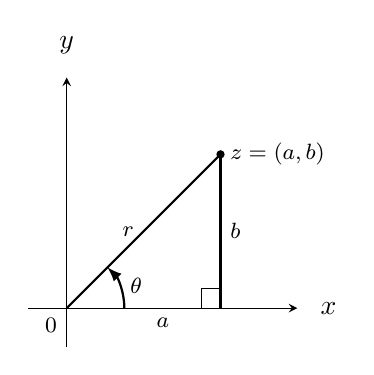
\begin{tikzpicture}
\begin{axis}[disabledatascaling, 
	clip mode=individual, 
    width=5cm, 
    height=5cm, 
    xlabel={$x$}, 
    ylabel={$y$}, 
    axis lines=middle, 
    xtick=\empty, 
    ytick=\empty, 
    xticklabels=\empty, 
    yticklabels=\empty, 
    every axis x label/.style={
      at={(ticklabel* cs:1.05)},
      anchor=west,
    },
    every axis y label/.style={
      at={(ticklabel* cs:1.05)},
      anchor=south,
    },
    domain=-5:5, 
    samples=100, 
    xmin=-0.5, 
    xmax=3, 
    ymin=-0.5, 
    ymax=3]
\draw[thick](0,0)--(2,2);
\fill[black] (2,2) circle (1.5pt);
\draw[thick,-latex] (0.75,0) arc [start angle=0,end angle=45,radius=0.75] node[right,text=black,font=\footnotesize,midway]{$\theta$};
\draw[thick](2,0)--(2,2);
\draw (1.75,0)--(1.75,0.25)--(2,0.25);
\node[below left,font=\footnotesize] at (0,0){$0$};
\node[below,font=\footnotesize] at (1.25,0){$a$};
\node[right,font=\footnotesize] at (2,1){$b$};
\node[left,font=\footnotesize] at (1,1){$r$};
\node[right,font=\footnotesize] at (2,2){$z=(a,b)$};
\end{axis} 
\end{tikzpicture}

	\caption{\label{fig:033977}}
\end{wrapfigure}
If $z \neq 0$, the angle $\theta$ shown in Figure~\ref{fig:033977} is called an \textbf{argument}\index{argument} of $z$ and is denoted
\begin{equation*}
\theta = \func{arg} z
\end{equation*} 
This angle is not unique ($\theta + 2\pi k$ would do as well for any \newline $k = 0, \pm 1, \pm 2, \dots$ ). However, there is only one argument $\theta$ in the range $-\pi < \theta \leq \pi$, and this is sometimes called the \textbf{principal argument}\index{principal argument} of $z$.

Returning to Figure~\ref{fig:033977}, we find that the real and imaginary parts $a$ and $b$ of $z$ are related to $r$ and $\theta$ by
\begin{align*}
a &= r \cos \theta \\
b &= r \sin \theta
\end{align*}
Hence the complex number $z = a + bi$ has the form
\begin{equation*}
z = r(\cos \theta + i \sin \theta) \quad r = |z|, \theta = \func{arg}(z)
\end{equation*}
The combination $\cos \theta + i \sin \theta$ is so important that a special notation is used:
\begin{equation*}
e^{i\theta} = \cos \theta + i \sin \theta
\end{equation*}
is called \textbf{Euler's formula}\index{Euler's formula} after the great Swiss mathematician Leonhard Euler (1707--1783)\index{Euler, Leonhard}. With this notation, $z$ is written
\begin{equation*}
z = r e^{i \theta} \quad r = |z|, \theta = \func{arg}(z)
\end{equation*}
This is a \textbf{polar form} of the complex number $z$. Of course it is not unique, because the argument can be changed by adding a multiple of $2\pi$.


\begin{example}{}{033987}
Write $z_{1} = -2 + 2i$ and $z_{2} = -i$ in polar form.


\begin{solution}
\begin{wrapfigure}[7]{l}{5cm}
	\centering
	
\begin{tikzpicture}
\begin{axis}[disabledatascaling, 
	clip mode=individual, 
    width=5cm, 
    height=5cm, 
    xlabel={$x$}, 
    ylabel={$y$}, 
    axis lines=middle, 
    xtick=\empty, 
    ytick=\empty, 
    xticklabels=\empty, 
    yticklabels=\empty, 
    every axis x label/.style={
      at={(ticklabel* cs:1.05)},
      anchor=west,
    },
    every axis y label/.style={
      at={(ticklabel* cs:1.05)},
      anchor=south,
    },
    domain=-5:5, 
    samples=100, 
    xmin=-2.1, 
    xmax=2.1, 
    ymin=-2.1, 
    ymax=2.1]
\draw[dkgreenvect,thick](0,0)--(-2,2);
\draw[dkgreenvect,thick](0,0)--(0,-1);
\draw[-latex] (0.75,0) arc [start angle=0,end angle=135,radius=0.75] node [right, text=black,font=\footnotesize,midway]{$\theta_1$};
\draw[-latex] (0.5,0) arc [start angle=0,end angle=270,radius=0.5] node [left, text=black,font=\footnotesize,pos=0.95]{$\theta_2$};
\fill[black] (-2,2) circle (1.5pt);
\fill[black] (0,-1) circle (1.5pt);
\node[below right,font=\footnotesize] at (0,0){$0$};
\node[above,font=\footnotesize] at (-2,2){$z_1=-2+2i$};
\node[right,font=\footnotesize] at (0,-1){$z_2=-i$};
\end{axis} 
\end{tikzpicture}

	\caption{\label{fig:033996}}	
\end{wrapfigure}

\setlength{\rightskip}{0pt plus 200pt}
The two numbers are plotted in the complex plane in Figure~\ref{fig:033996}. The absolute values are
\begin{align*}
r_1 &= |-2 + 2i| = \sqrt{(-2)^2 + 2^2} = 2\sqrt{2}\\
r_2 &= |-i| = \sqrt{0^2 + (-1)^2} = 1
\end{align*}
By inspection of Figure~\ref{fig:033996}, arguments of $z_{1}$ and $z_{2}$ are
\begin{align*}
\theta_1 &= \func{arg}(-2+2i) = \frac{3\pi}{4}\\
\theta_2 &= \func{arg}(-i) = \frac{3\pi}{2}
\end{align*}
The corresponding polar forms are $z_{1} = -2 + 2i = 2\sqrt{2} e^{3\pi i/4}$
 and $z_{2} = -i = e^{3\pi i/2}$. Of course, we could have taken the argument $-\frac{\pi}{2}$ for $z_{2}$ and obtained the polar form $z_{2} = e^{-\pi i/2}$.
\end{solution}
\end{example}

In Euler's formula $e^{i\theta}= \cos \theta + i \sin \theta$, the number $e$ is the familiar constant $e = 2.71828\dots$  from calculus. The reason for using $e$ will not be given here; the reason why $\cos \theta + i \sin \theta$ is written as an \textit{exponential} function of $\theta$ is that the \textbf{law of exponents}\index{law of exponents} holds:
\begin{equation*}
e^{i\theta} \cdot e^{i\phi} = e^{i (\theta + \phi)}
\end{equation*}
where $\theta$ and $\phi$ are any two angles. In fact, this is an immediate consequence of the addition identities for $\sin(\theta + \phi)$ and $\cos(\theta + \phi)$:
\newpage
\begin{align*}
e^{i\theta} e^{i\phi} &= (\cos \theta + i \sin \theta) (\cos \phi + i \sin \phi) \\
&= (\cos \theta \cos \phi - \sin \theta \sin \phi) + i (\cos \theta \sin \phi + \sin \theta \cos \phi) \\
&= \cos (\theta +  \phi) +i \sin (\theta + \phi) \\
& =e^{i (\theta + \phi)}
\end{align*}
This is analogous to the rule $e^{a}e^{b} = e^{a+b}$, which holds for real numbers $a$ and $b$, so it is not unnatural to use the exponential notation $e^{i\theta}$ for the expression $\cos \theta + i \sin \theta$. In fact, a whole theory exists wherein functions such as $e^{z}$, $\sin z$, and $\cos z$ are studied, where $z$ is a \textit{complex}
 variable. Many deep and beautiful theorems can be proved in this 
theory, one of which is the so-called fundamental theorem of algebra 
mentioned later (Theorem~\ref{thm:034196}). We shall not pursue this here.


The geometric description of the multiplication of two complex numbers follows from the law of exponents.


\begin{theorem}{Multiplication Rule}{034029}
If $z_{1} = r_{1}e^{i{\theta}_1}$ and $z_{2} = r_{2}e^{i{\theta}_2}$ are complex numbers in polar form, then
\begin{equation*}
z_1z_2 = r_1r_2e^{i (\theta_1 + \theta_2)}
\end{equation*}\index{multiplication rule}
\vspace*{-2em}
\end{theorem}

\noindent In other words, to multiply two complex
 numbers, simply multiply the absolute values and add the arguments. 
This simplifies calculations considerably, particularly when we observe 
that it is valid for \textit{any} arguments $\theta_{1}$ and $\theta_{2}$.


\begin{example}{}{034047}
Multiply $(1-i)(1+\sqrt{3}i)$ in two ways.


\begin{solution}
\begin{wrapfigure}[8]{l}{5cm}
	\centering
	
\begin{tikzpicture}
\begin{axis}[disabledatascaling, 
	clip mode=individual, 
    width=5cm, 
    height=5cm, 
    xlabel={$x$}, 
    ylabel={$y$}, 
    axis lines=middle, 
    xtick=\empty, 
    ytick=\empty, 
    xticklabels=\empty, 
    yticklabels=\empty, 
    every axis x label/.style={
      at={(ticklabel* cs:1.05)},
      anchor=west,
    },
    every axis y label/.style={
      at={(ticklabel* cs:1.05)},
      anchor=south,
    },
    domain=-5:5, 
    samples=100, 
    xmin=-0.25, 
    xmax=3, 
    ymin=-2.1, 
    ymax=2.5]
\draw[dkgreenvect,thick](0,0)--(1,1.73);
\draw[-latex] (0.5,0) arc [start angle=0,end angle=60,radius=0.5] node [right, text=black,font=\scriptsize,pos=0.8]{$\frac{\pi}{3}$};
\draw[dkgreenvect,thick](0,0)--(1,-1);
\draw[-latex] (0.75,0) arc [start angle=0,end angle=-45,radius=0.75] node [right, text=black,font=\scriptsize,midway]{$-\frac{\pi}{4}$};
\draw[dkgreenvect,thick](0,0)--(2.73,0.73);
\draw[-latex] (2,0) arc [start angle=0,end angle=15,radius=2] node [right, text=black,font=\scriptsize,midway]{$\frac{\pi}{12}$};
\fill[dkgreenvect] (1,1.73) circle (1.5pt);
\fill[dkgreenvect] (1,-1) circle (1.5pt);
\fill[dkgreenvect] (2.73,0.73) circle (1.5pt);
\node[below left,font=\scriptsize] at (0,0){$0$};
\node[above,font=\scriptsize] at (1,1.73){$1+\sqrt{3}i$};
\node[below,font=\scriptsize] at (1,-1){$1-i$};
\node[above,font=\scriptsize] at (2.5,0.73){$(1-i)(1+\sqrt{3}i)$};
\end{axis} 
\end{tikzpicture}

	\caption{\label{fig:034054}}
\end{wrapfigure}
	
\setlength{\rightskip}{0pt plus 200pt}
  We have $|1 - i| = \sqrt{2}$ and $|1 + \sqrt{3}i| = 2$ so, from Figure~\ref{fig:034054},
\begin{align*}
& 1-i = \sqrt{2} e^{-i\pi /4} \\
& 1+ \sqrt{3}i = 2e^{i\pi /3}
\end{align*}

Hence, by the multiplication rule,
\begin{align*}
(1-i)(1+\sqrt{3}i) &= (\sqrt{2} e^{-i\pi /4})(2e^{i\pi /3}) \\
&= 2\sqrt{2} e^{i(-\pi/4 + \pi/3)} \\
&= 2 \sqrt{2} e^{i\pi/12}
\end{align*}

This gives the required product in polar form. Of course, direct multiplication gives $(1 - i)(1 + \sqrt{3}i) = (\sqrt{3} + 1) + (\sqrt{3} - 1)i$. Hence, equating real and imaginary parts gives the formulas $\cos (\frac{\pi}{12}) = \frac{\sqrt{3}+1}{2\sqrt{2}}$ and $\sin (\frac{\pi}{12}) = \frac{\sqrt{3}-1}{2\sqrt{2}}$.
\end{solution}
\end{example}

\subsection*{Roots of Unity}

If a complex number $z = re^{i\theta}$ is given in polar form, the powers assume a particularly simple form. In fact, $z^{2} = (re^{i\theta})(re^{i\theta}) = r^{2}e^{2i\theta}$, $z^{3} = z^{2} \cdot z = (r^{2}e^{2i\theta})(re^{i\theta}) = r^{3}e^{3i\theta}$, and so on. Continuing in this way, it follows by induction that the following theorem holds for any positive integer $n$. The name honours Abraham De Moivre (1667--1754).\index{complex number!roots of unity}\index{De Moivre, Abraham}\index{roots of unity}


\begin{theorem}{De Moivre's Theorem}{034080}
If $\theta$ is any angle, then $(e^{i\theta})^{n} = e^{in\theta}$ holds for all integers $n$.\index{De Moivre's Theorem}
\end{theorem}

\begin{proof}
The case $n > 0$ has been discussed, and the reader can verify the result for $n = 0$. To derive it for $n < 0$, first observe that
\begin{equation*}
\mbox{if } \quad z = re^{i\theta}\neq 0 \quad \mbox{ then } \quad z^{-1} = \frac{1}{r}~e^{-i\theta}
\end{equation*}
In fact, $(re^{i\theta})(\frac{1}{r} e^{-i\theta}) = 1e^{i0} = 1$ by the multiplication rule. Now assume that $n$ is negative and write it as $n = -m$, $m > 0$. Then
\begin{equation*}
(re^{i\theta})^n = [(re^{i\theta})^{-1}]^m = (\frac{1}{r}~e^{-i\theta})^m = r^{-m} e^{i(-m\theta)}=r^ne^{in\theta}
\end{equation*}
If $r = 1$, this is De Moivre's theorem for negative $n$.
\end{proof}

\begin{example}{}{034096}
\begin{wrapfigure}{l}{5cm}
        \vspace*{-1.5em}
	\centering
	
\begin{tikzpicture}%[scale=0.75]
\begin{axis}[disabledatascaling, 
	clip mode=individual, 
    width=5cm, 
    height=5cm, 
    xlabel={$x$}, 
    ylabel={$y$}, 
    axis lines=middle, 
    xtick=\empty, 
    ytick=\empty, 
    xticklabels=\empty, 
    yticklabels=\empty, 
    every axis x label/.style={
      at={(ticklabel* cs:1.05)},
      anchor=west,
    },
    every axis y label/.style={
      at={(ticklabel* cs:1.05)},
      anchor=south,
    },
    domain=-5:5, 
    samples=100, 
    xmin=-2, 
    xmax=2, 
    ymin=-0.5, 
    ymax=2]
\draw[dkgreenvect,thick](0,0)--(-1,1.73);
\draw[-latex] (0.75,0) arc [start angle=0,end angle=120,radius=0.75] node [right, text=black,font=\scriptsize,midway]{$\frac{2\pi}{3}$};
\fill[dkgreenvect] (-1,1.73) circle (1.5pt);
\node[below left,font=\scriptsize] at (0,0){$0$};
\node[above,font=\scriptsize] at (-1,1.73){$-1+\sqrt{3}i$};
\node[below left,font=\scriptsize] at (-0.5,0.865){$2$};
\end{axis} 
\end{tikzpicture}

	\caption{\label{fig:034105}}
\end{wrapfigure}

\setlength{\rightskip}{0pt plus 200pt}
Verify that $(-1+\sqrt{3}i)^3 = 8$.

\begin{solution}
  We have $| -1 + \sqrt{3}i| =2$, so $-1 + \sqrt{3}i = 2e^{2\pi i /3}$ (see Figure~\ref{fig:034105}). Hence De Moivre's theorem gives
\begin{equation*}
(-1+\sqrt{3}i)^3 = (2e^{2\pi i /3})^3 = 8e^{3(2\pi i /3)} = 8e^{2\pi i} = 8
\end{equation*}
\vspace{3em}
\end{solution}
\end{example}

De Moivre's theorem can be used to find $n$th roots of complex numbers where $n$ is positive. The next example illustrates this technique.


\begin{example}{}{034107}
Find the cube roots of unity; that is, find all complex numbers $z$ such that $z^{3} = 1$.


\begin{solution}
  First write $z = re^{i\theta}$ and $1 = 1e^{i0}$ in polar form. We must use the condition $z^{3} = 1$ to determine $r$ and $\theta$. Because $z^{3} = r^{3}e^{3i\theta}$ by De Moivre's theorem, this requirement becomes
\begin{equation*}
r^3 e^{3i\theta} = 1 e^{0i}
\end{equation*}
These two complex numbers are equal, so
 their absolute values must be equal and the arguments must either be 
equal or differ by an integral multiple of $2\pi$:
\begin{align*}
r^3 & = 1 \\
3 \theta &= 0 +2k\pi, \quad k \mbox{ some integer} 
\end{align*}
Because $r$ is real and positive, the condition $r^{3} = 1$ implies that $r = 1$. However,
\begin{equation*}
\theta = \frac{2k\pi}{3}, \quad k \mbox{ some integer}
\end{equation*}
\begin{wrapfigure}[8]{l}{5cm}
        \vspace*{-2em}
	\centering
	
\begin{tikzpicture}
\begin{axis}[disabledatascaling, 
	clip mode=individual, 
    width=5cm, 
    height=5cm, 
    xlabel={$x$}, 
    ylabel={$y$}, 
    axis lines=middle, 
    xtick={-5,-4,...,5}, 
    ytick={-5,-4,...,5}, 
    xticklabels=\empty, 
    yticklabels=\empty, 
    every axis x label/.style={
      at={(ticklabel* cs:1.05)},
      anchor=west,
    },
    every axis y label/.style={
      at={(ticklabel* cs:1.05)},
      anchor=south,
    },
    domain=-5:5, 
    samples=100, 
    xmin=-1.5, 
    xmax=1.5, 
    ymin=-1.5, 
    ymax=1.5]
\draw (0,0) circle (1); 
\draw[-latex] (0.5,0) arc [start angle=0,end angle=120,radius=0.5] node [right, text=black,font=\footnotesize,midway]{$\frac{2\pi}{3}$};
\draw[dkgreenvect,thick](0,0)--(-0.5,0.866);
\draw[-latex] (0.25,0) arc [start angle=0,end angle=240,radius=0.25] node [left, text=black,font=\footnotesize,pos=0.95]{$\frac{4\pi}{3}$};
\draw[dkgreenvect,thick](0,0)--(-0.5,-0.866);
\fill[black] (1,0) circle (1.5pt);
\fill[black] (-0.5,0.866) circle (1.5pt);
\fill[black] (-0.5,-0.866) circle (1.5pt);
\node[below right,font=\footnotesize] at (0,0){$0$};
\node[below right,font=\footnotesize] at (1,0){$1$};
\node[above left,font=\footnotesize] at (-0.5,0.866){$-\frac{1}{2}+\frac{\sqrt{3}}{2}i$};
\node[below left,font=\footnotesize] at (-0.5,-0.866){$-\frac{1}{2}-\frac{\sqrt{3}}{2}i$};
\end{axis} 
\end{tikzpicture}

	\caption{\label{fig:034128}}
\end{wrapfigure}
\setlength{\rightskip}{0pt plus 200pt}
seems at first glance to yield infinitely many different angles for $z$. However, choosing $k = 0, 1, 2$ gives three possible arguments $\theta$ (where $0 \leq \theta < 2\pi$), and the corresponding roots are
\begin{align*}
1e^{0i} & = 1 \\
1e^{2\pi i/3} & = -\frac{1}{2} + \frac{\sqrt{3}}{2} i \\
1e^{4\pi i/3} & = -\frac{1}{2} - \frac{\sqrt{3}}{2} i
\end{align*}
These are displayed in Figure~\ref{fig:034128}. All other values of $k$
 yield values of $\theta$ that differ from one of these by a multiple of $2\pi$---and
 so do not give new roots. Hence we have found all the roots.
\end{solution}
\end{example}

The same type of calculation gives all complex $n$\textbf{th roots of unity}; that is, all complex numbers $z$ such that $z^n = 1$. As before, write $1 = 1e^{0i}$ and
\begin{equation*}
z = re^{i\theta}
\end{equation*}
in polar form. Then $z^n = 1$ takes the form
\begin{equation*}
r^ne^{ni\theta} = 1e^{0i}
\end{equation*}
using De Moivre's theorem. Comparing absolute values and arguments yields
\begin{align*}
r^n &= 1 \\
n\theta & = 0 + 2k\pi, \quad k \mbox{ some integer}
\end{align*}
Hence $r = 1$, and the $n$ values
\begin{equation*}
\theta = \frac{2k\pi}{n}, \quad k=0, 1, 2, \dots, n-1
\end{equation*}
of $\theta$ all lie in the range $0 \leq \theta < 2\pi$. As in Example~\ref{exa:034107}, \textit{every} choice of $k$ yields a value of $\theta$ that differs from one of these by a multiple of $2\pi$, so these give the arguments of \textit{all} the possible roots.


\begin{theorem}{$n$th Roots of Unity}{034138}
If $n \geq 1$ is an integer, the $n$th roots of unity (that is, the solutions to $z^n = 1$) are given by
\begin{equation*}
z = e^{2\pi ki/n}, \quad k = 0, 1, 2, \dots, n-1
\end{equation*}\index{$n$th roots of unity}
\vspace*{-2em}
\end{theorem}

\begin{wrapfigure}[6]{l}{5cm}
        \vspace*{-1em}
	\centering
	
\begin{tikzpicture}[scale=0.9]
\begin{axis}[disabledatascaling, 
	clip mode=individual, 
    width=5cm, 
    height=5cm, 
    xlabel={$x$}, 
    ylabel={$y$}, 
    axis lines=middle, 
    xtick={-5,-4,...,5}, 
    ytick={-5,-4,...,5}, 
    xticklabels=\empty, 
    yticklabels=\empty, 
    every axis x label/.style={
      at={(ticklabel* cs:1.05)},
      anchor=west,
    },
    every axis y label/.style={
      at={(ticklabel* cs:1.05)},
      anchor=south,
    },
    domain=-5:5, 
    samples=100, 
    xmin=-1.5, 
    xmax=1.5, 
    ymin=-1.5, 
    ymax=1.5]
\draw (0,0) circle (1); 
\draw[dkgreenvect,thick](0,0)--(1,0);
\draw[dkgreenvect,thick](0,0)--(0.309,0.951);
\draw[dkgreenvect,thick](0,0)--(-0.809,0.588);
\draw[dkgreenvect,thick](0,0)--(-0.809,-0.588);
\draw[dkgreenvect,thick](0,0)--(0.309,-0.951);


\fill[black] (1,0) circle (1.5pt);
\fill[black] (0.309,0.951) circle (1.5pt);
\fill[black] (-0.809,0.588) circle (1.5pt);
\fill[black] (-0.809,-0.588) circle (1.5pt);
\fill[black] (0.309,-0.951) circle (1.5pt);

\node[below right,font=\footnotesize] at (0,0){$0$};
\node[above right,font=\footnotesize] at (0.9,0){$1=e^{0i}$};
\node[above right,font=\footnotesize] at (0.309,0.951){$e^{2\pi i/5}$};
\node[left,font=\footnotesize] at (-0.809,0.588){$e^{4\pi i/5}$};
\node[below left,font=\footnotesize] at (-0.809,-0.588){$e^{6\pi i/5}$};
\node[below right,font=\footnotesize] at (0.309,-0.951){$e^{8\pi i/5}$};
\end{axis} 
\end{tikzpicture}

	\caption{\label{fig:034146}}
\end{wrapfigure}

\noindent The $n$th roots of unity can be found geometrically as the points on the unit circle that cut the circle into $n$ equal sectors, starting at $1$. The case $n = 5$ is shown in Figure~\ref{fig:034146}, where the five fifth roots of unity are plotted.

\vspace{2em}

The method just used to find the $n$th roots of unity works equally well to find the $n$th roots of any complex number in polar form. We give one example.

\begin{example}{}{034148}
Find the fourth roots of $\sqrt{2} + \sqrt{2}i$.


\begin{solution}
  First write $\sqrt{2} + \sqrt{2}i = 2e^{\pi i/4}$ in polar form. If $z = re^{i\theta}$ satisfies $z^{4} = \sqrt{2} + \sqrt{2}i$, then De Moivre's theorem gives
\begin{equation*}
r^4e^{i(4\theta)} = 2e^{\pi i/4}
\end{equation*}
Hence $r^{4} = 2$ and $4\theta = \frac{\pi}{4} + 2k\pi$, $k$ an integer. We obtain four distinct roots (and hence all) by
\begin{equation*}
r = \sqrt[4]{2}, \quad \theta = \frac{\pi}{16} = \frac{2k\pi}{16}, k=0, 1, 2, 3
\end{equation*}
Thus the four roots are
\begin{equation*}
\sqrt[4]{2} e^{\pi i/16} \quad  \sqrt[4]{2} e^{9\pi i/16} \quad \sqrt[4]{2} e^{17 \pi i/16} \quad \sqrt[4]{2} e^{25\pi i/16}
\end{equation*}
Of course, reducing these roots to the form $a + bi$ would require the computation of $\sqrt[4]{2}$
 and the sine and cosine of the various angles.
\end{solution}
\end{example}

An expression of the form $ax^{2} + bx + c$, where the coefficients $a \neq 0$, $b$, and $c$ are real numbers, is called a \textbf{real quadratic}\index{real quadratic}. A complex number $u$ is called a \textbf{root}\index{root!of the quadratic} of the quadratic if $au^{2} + bu + c = 0$. The roots are given by the famous \textbf{quadratic formula}\index{quadratic formula}:
\begin{equation*}
u = \frac{-b \pm \sqrt{b^2 - 4ac}}{2a}
\end{equation*}
The quantity $d = b^{2} - 4ac$ is called the \textbf{discriminant}\index{discriminant} of the quadratic $ax^{2} + bx + c$, and there is no real root if and only if $d < 0$. In this case the quadratic is said to be \textbf{irreducible}\index{irreducible}. Moreover, the fact that $d < 0$ means that $\sqrt{d} = i\sqrt{|d|}$, so the two (complex) roots are conjugates of each other:
\begin{equation*}
u = \frac{1}{2a}(-b+i\sqrt{|d|}) \quad \mbox{ and } \quad \overline{u} = \frac{1}{2a}(-b-i\sqrt{|d|})
\end{equation*}
The converse of this is true too: Given any nonreal complex number $u$, then $u$ and $\overline{u}$
 are the roots of some real irreducible quadratic. Indeed, the quadratic
\begin{equation*}
x^2 - (u + \overline{u})x + u \overline{u} = (x-u)(x-\overline{u})
\end{equation*}
has real coefficients ($u\overline{u} = |u|^{2}$ and $u + \overline{u}$
 is twice the real part of $u$) and so is irreducible because its roots $u$ and $\overline{u}$
 are not real.


\begin{example}{}{034182}
Find a real irreducible quadratic with $u = 3 - 4i$ as a root.


\begin{solution}
  We have $u + \overline{u} = 6$ and $|u|^{2} = 25$, so $x^{2} - 6x + 25$ is irreducible with $u$ and $\overline{u} = 3 + 4i$ as roots.
\end{solution}
\end{example}

\subsection*{Fundamental Theorem of Algebra}

As we mentioned earlier, the complex 
numbers are the culmination of a long search by mathematicians to find a
 set of numbers large enough to contain a root of every polynomial. The 
fact that the complex numbers have this property was first proved by 
Gauss in 1797 when he was 20 years old. The proof is omitted.


\begin{theorem}{Fundamental Theorem of Algebra}{034196}
Every polynomial of positive degree with complex coefficients has a complex root.
\end{theorem}

\noindent If $f(x)$ is a polynomial with complex coefficients, and if $u_{1}$ is a root, then the factor theorem (Section~\ref{sec:6_5}) asserts that
\begin{equation*}
f(x) = (x-u_1)g(x)
\end{equation*}
where $g(x)$ is a polynomial with complex coefficients and with degree one less than the degree of $f(x)$. Suppose that $u_{2}$ is a root of $g(x)$, again by the fundamental theorem. Then $g(x) = (x - u_{2})h(x)$, so
\begin{equation*}
f(x) = (x-u_1)(x-u_2)h(x)
\end{equation*}
This process continues until the last polynomial to appear is linear. Thus $f(x)$ has been expressed as a product of linear factors. The last of these factors can be written in the form $u(x - u_{n})$, where $u$ and $u_{n}$ are complex (verify this), so the fundamental theorem takes the following form.


\begin{theorem}{}{034210}
Every complex polynomial $f(x)$ of degree $n \geq 1$ has the form
\begin{equation*}
f(x) = u(x-u_1)(x-u_2)\cdots (x-u_n)
\end{equation*}
where $u, u_{1}, \dots, u_{n}$ are complex numbers and $u \neq 0$. The numbers $u_{1}, u_{2}, \dots, u_{n}$ are the roots of $f(x)$ (and need not all be distinct), and $u$ is the coefficient of $x^{n}$.
\end{theorem}

\noindent This form of the fundamental theorem, when applied to a polynomial $f(x)$ with \textit{real} coefficients, can be used to deduce the following result.


\begin{theorem}{}{034221}
Every polynomial $f(x)$ of positive 
degree with real coefficients can be factored as a product of linear and
 irreducible quadratic factors.
\end{theorem}

\noindent In fact, suppose $f(x)$ has the form
\begin{equation*}
f(x) = a_nx^n + a_{n-1}x^{n-1} + \cdots + a_1x + a_0
\end{equation*}
where the coefficients $a_{i}$ are real. If $u$ is a complex root of $f(x)$, then we claim first that $\overline{u}$
 is also a root. In fact, we have $f(u) = 0$, so
\begin{align*}
0 = \overline{0} = \overline{f(u)} & = \overline{a_nu^n + a_{n-1}u^{n-1} + \cdots + a_1u + a_0 } \\
& = \overline{a_nu^n} + \overline{a_{n-1}u^{n-1}} + \cdots + \overline{a_1u} + \overline{a_0 } \\
& = \overline{a}_n\overline{u}^n + \overline{a}_{n-1}\overline{u}^{n-1} + \cdots + \overline{a}_1\overline{u} + \overline{a}_0 \\
& = a_n\overline{u}^n + a_{n-1}\overline{u}^{n-1} + \cdots + a_1\overline{u} + a_0 \\
&= f(\overline{u})
\end{align*}
where $\overline{a}_i = a_i$
 for each $i$ because the coefficients $a_{i}$ are real. Thus if $u$ is a root of $f(x)$, so is its conjugate $\overline{u}$. Of course some of the roots of $f(x)$ may be real (and so equal their conjugates), but the nonreal roots come in pairs, $u$ and $\overline{u}$. By Theorem~\ref{thm:034221}, we can thus write $f(x)$ as a product:
\begin{equation}\label{eq:complexproduct}
f(x) = a_n(x-r_1)\cdots(x-r_k)(x-u_1)(x-\overline{u}_1)\cdots (x-u_m)(x-\overline{u}_m)
\end{equation}
where $a_{n}$ is the coefficient of $x^{n}$ in $f(x)$; $r_{1}, r_{2}, \dots , r_{k}$ are the real roots; and $u_{1}, \overline{u}_{1}, u_{2}, \overline{u}_{2}, \dots , u_{m}, \overline{u}_{m}$ are the nonreal roots. But the product
\begin{equation*}
(x-u_j)(x-\overline{u}_j) = x^2 - (u_j + \overline{u}_j)x +(u_j \overline{u}_j)
\end{equation*}
is a real irreducible quadratic for each $j$ (see the discussion preceding Example~\ref{exa:034182}). Hence (\ref{eq:complexproduct}) shows that $f(x)$ is a product of linear and irreducible quadratic factors, each with real coefficients. This is the conclusion in Theorem~\ref{thm:034221}.


\section*{Exercises for \ref{chap:appacomplexnumbers}}

\begin{Filesave}{solutions}
\solsection{Appendix~\ref{chap:appacomplexnumbers}}
\end{Filesave}

\begin{multicols}{2}
\begin{ex}
Solve each of the following for the real number $x$.

\begin{exenumerate}
\exitem $x-4i = (2-i)^2$
\exitem $(2+xi)(3-2i) \\ \hspace*{2em}= 12+5i$
\exitem $(2+xi)^2=4$
\exitem $(2+xi)(2-xi)=5$
\end{exenumerate}
\begin{sol}
\begin{enumerate}[label={\alph*.}]
\setcounter{enumi}{1}
\item $x = 3$

\setcounter{enumi}{3}
\item  $x = \pm 1$

\end{enumerate}
\end{sol}
\end{ex}

\columnbreak

\begin{ex}
Convert each of the following to the form $a + bi$.

\begin{exenumerate}
\exitem* $(2-3i)-2(2-3i)+9$
\exitem*  $(3-2i)(1+i)+|3+4i|$
\exitem $\frac{1+i}{2-3i} + \frac{1-i}{-2+3i}$
\exitem $\frac{3-2i}{1-i} + \frac{3-7i}{2-3i}$
\exitem $i^{131}$
\exitem $(2 - i)^{3}$
\exitem $(1 + i)^{4}$
\exitem $(1 - i)^{2}(2 + i)^{2}$
\exitem* $\frac{3\sqrt{3}-i}{\sqrt{3}+i} + \frac{\sqrt{3}+7i}{\sqrt{3}-i}$
\end{exenumerate}
\begin{sol}
\begin{enumerate}[label={\alph*.}]
\setcounter{enumi}{1}
\item  $10 + i$

\setcounter{enumi}{3}
\item $\frac{11}{26} + \frac{23}{26}i$


\setcounter{enumi}{5}
\item $ 2 - 11i$

\setcounter{enumi}{7}
\item  $8 - 6i$

\end{enumerate}
\end{sol}
\end{ex}

\begin{ex}
In each case, find the complex number $z$.

\begin{exenumerate}
\exitem $ iz - (1 + i)^{2} = 3 - i$
\exitem* $(i + z) - 3i(2 - z) = iz + 1$
\exitem $z^{2} = -i$
\exitem $z^{2} = 3 - 4i$
\exitem $z(1+i) = \overline{z} + (3+2i)$
\exitem* $z(2-i) = (\overline{z}+1)(1+i)$
\end{exenumerate}
\begin{sol}
\begin{enumerate}[label={\alph*.}]
\setcounter{enumi}{1}
\item $\frac{11}{5} + \frac{3}{5}i$


\setcounter{enumi}{3}
\item  $\pm(2 - i)$

\setcounter{enumi}{5}
\item $ 1 + i$

\end{enumerate}
\end{sol}
\end{ex}

\begin{ex}
In each case, find the roots of the real quadratic equation.

\begin{exenumerate}
\exitem  $x^{2} - 2x + 3 = 0$
\exitem  $x^{2} - x + 1 = 0$
\exitem $3x^{2} - 4x + 2 = 0$
\exitem  $2x^{2} - 5x + 2 = 0$
\end{exenumerate}
\begin{sol}
\begin{enumerate}[label={\alph*.}]
\setcounter{enumi}{1}
\item $\frac{1}{2} \pm \frac{\sqrt{3}}{2}i$


\setcounter{enumi}{3}
\item  $2$, $\frac{1}{2}$

\end{enumerate}
\end{sol}
\end{ex}

\begin{ex}
Find all numbers $x$ in each case.

\begin{exenumerate}
\exitem $x^{3} = 8$
\exitem $x^{3} = -8$
\exitem  $x^{4} = 16$
\exitem  $x^{4} = 64$
\end{exenumerate}
\begin{sol}
\begin{enumerate}[label={\alph*.}]
\setcounter{enumi}{1}
\item  $-2$, $1 \pm \sqrt{3}i$


\setcounter{enumi}{3}
\item  $\pm 2\sqrt{2}$, $\pm 2\sqrt{i}$


\end{enumerate}
\end{sol}
\end{ex}

\begin{ex}
In each case, find a real quadratic with $u$ as a root, and find the other root.

\begin{exenumerate}
\exitem  $u = 1 + i$
\exitem  $u = 2 - 3i$
\exitem $u = -i$
\exitem $u = 3 - 4i$
\end{exenumerate}
\begin{sol}
\begin{enumerate}[label={\alph*.}]
\setcounter{enumi}{1}
\item  $x^{2} - 4x + 13$; $2 + 3i$

\setcounter{enumi}{3}
\item  $x^{2} - 6x + 25$; $3 + 4i$

\end{enumerate}
\end{sol}
\end{ex}

\begin{ex}
Find the roots of $x^{2} - 2\cos \theta x + 1 = 0$, $\theta$ any angle.
\end{ex}

\begin{ex}
Find a real polynomial of degree $4$ with $2 - i$ and $3 - 2i$ as roots.

\begin{sol}
$x^{4} - 10x^{3} + 42x^{2} - 82x + 65$
\end{sol}
\end{ex}

\begin{ex}
Let $\func{re }z$ and $\func{im }z$ denote, respectively, the real and imaginary parts of $z$. Show that:

\begin{exenumerate}
\exitem $\func{im}(iz) = \func{re }z$
\exitem $\func{re}(iz) = -\func{im }z$
\exitem $z + \overline{z} = 2 \func{re}z$
\exitem $z - \overline{z} = 2i \func{im} z$
\exitem* $\func{re}(z + w) = \func{re }z + \func{re }w$, and $\func{re}(tz) = t \cdot \func{re }z$ if $t$ is real
\exitem* $\func{im}(z + w) = \func{im }z + \func{im }w$, and $\func{im}(tz) = t \cdot \func{im }z$ if $t$ is real
\end{exenumerate}
\end{ex}

\columnbreak 
\begin{ex}
In each case, show that $u$ is a root of the quadratic equation, and find the other root.\index{complex number!root of the quadratic}

\begin{exenumerate}
\exitem* $x^{2} - 3ix + (-3 + i) = 0$; $u = 1 + i$
\exitem* $x^{2} + ix - (4 - 2i) = 0$; $u = -2$
\exitem* $x^{2} - (3 - 2i)x + (5 - i) = 0$; $u = 2 - 3i$
\exitem* $x^{2} + 3(1 - i)x - 5i = 0$; $u = -2 + i$
\end{exenumerate}
\begin{sol}
\begin{enumerate}[label={\alph*.}]
\setcounter{enumi}{1}
\item  $(-2)^{2} + 2i - (4 - 2i) = 0$; $2 - i$

\setcounter{enumi}{3}
\item  $(-2 + i)^{2} + 3(1 - i)(-1 + 2i) - 5i = 0$; $-1 + 2i$

\end{enumerate}
\end{sol}
\end{ex}

\begin{ex}
Find the roots of each of the following complex quadratic equations.

\begin{exenumerate}
\exitem $x^{2} + 2x + (1 + i) = 0$
\exitem  $x^{2} - x + (1 - i) = 0$
\exitem* $x^{2} - (2 - i)x + (3 - i) = 0$
\exitem* $x^{2} - 3(1 - i)x - 5i = 0$
\end{exenumerate}
\begin{sol}
\begin{enumerate}[label={\alph*.}]
\setcounter{enumi}{1}
\item  $-i$, $1 + i$

\setcounter{enumi}{3}
\item  $2 - i$, $1 - 2i$

\end{enumerate}
\end{sol}
\end{ex}

\begin{ex}
In each case, describe the graph of the equation (where $z$ denotes a complex number).

\begin{exenumerate}
\exitem $|z| = 1$
\exitem $|z - 1| = 2$
\exitem $z = i \overline{z}$
\exitem $z = -\overline{z}$
\exitem $z = |z|$
\exitem $\func{im }z = m \cdot \func{re }z$, $m$ a real number
\end{exenumerate}
\begin{sol}
\begin{enumerate}[label={\alph*.}]
\setcounter{enumi}{1}
\item  Circle, centre at $1$, radius $2$

\setcounter{enumi}{3}
\item  Imaginary axis

\setcounter{enumi}{5}
\item  Line $y = mx$

\end{enumerate}
\end{sol}
\end{ex}

\begin{ex}
\begin{enumerate}[label={\alph*.}]
\item Verify $|zw| = |z||w|$ directly for $z = a + bi$ and $w = c + di$.

\item Deduce (a) from properties C2 and C6.

\end{enumerate}
\end{ex}

\begin{ex}
Prove that $|z+w| = |z|^2 + |w|^2 + w\overline{z} + \overline{w}z$
 for all complex numbers $w$ and $z$.
\end{ex}

\begin{ex}
If $zw$ is real and $z \neq 0$, show that $w = a \overline{z}$
 for some real number $a$.
\end{ex}

\begin{ex}
If $zw = \overline{z}v$
 and $z \neq 0$, show that $w = uv$ for some $u$ in $\mathbb{C}$  with $|u| = 1$.
\end{ex}

\begin{ex}
Show that $(1 + i)^{n} + (1 - i)^{n}$ is real for all $n$, using property C5.
\end{ex}

\begin{ex}
Express each of the following in polar form (use the principal argument).

\begin{exenumerate}
\exitem $3 - 3i$
\exitem $-4i$
\exitem $-\sqrt{3} + i$
\exitem $-4 + 4\sqrt{3}i$
\exitem $-7i$
\exitem $-6 + 6i$
\end{exenumerate}
\begin{sol}
\begin{enumerate}[label={\alph*.}]
\setcounter{enumi}{1}
\item  $4e^{-\pi i/2}$

\setcounter{enumi}{3}
\item  $8e^{2\pi i/3}$

\setcounter{enumi}{5}
\item  $6\sqrt{2}e^{3\pi i/4}$


\end{enumerate}
\end{sol}
\end{ex}

\columnbreak

\begin{ex}
Express each of the following in the form $a + bi$.

\begin{exenumerate}
\exitem $3e^{\pi i}$
\exitem $e^{7\pi i/3}$
\exitem $2e^{3 \pi i/4}$
\exitem $\sqrt{2}e^{-\pi i/4}$
\exitem $e^{5\pi i/4}$
\exitem $2\sqrt{3}e^{-2\pi i/6}$
\end{exenumerate}
\begin{sol}
\begin{enumerate}[label={\alph*.}]
\setcounter{enumi}{1}
\item  $\frac{1}{2} + \frac{\sqrt{3}}{2} i$

\setcounter{enumi}{3}
\item  $1 - i$

\setcounter{enumi}{5}
\item $\sqrt{3} - 3i$


\end{enumerate}
\end{sol}
\end{ex}

\begin{ex}
Express each of the following in the form $a + bi$.

\begin{exenumerate}
\exitem $(-1 + \sqrt{3}i)^2$
\exitem $(1 + \sqrt{3}i)^{-4}$
\exitem $(1 + i)^8$
\exitem $(1 - i)^{10}$
\exitem $(1 - i)^{6}(\sqrt{3} + i)^{3}$
\exitem $(\sqrt{3} - i)^{9}(2 - 2i)^{5}$
\end{exenumerate}
\begin{sol}
\begin{enumerate}[label={\alph*.}]
\setcounter{enumi}{1}
\item  $-\frac{1}{32} + \frac{\sqrt{3}}{32}i$


\setcounter{enumi}{3}
\item  $-32i$

\setcounter{enumi}{5}
\item  $-2^{16}(1 + i)$

\end{enumerate}
\end{sol}
\end{ex}

\begin{ex}
Use De Moivre's theorem to show that:

\begin{enumerate}[label={\alph*.}]
\item $\cos 2\theta = \cos^{2} \theta - \sin^{2} \theta$; $\sin 2\theta = 2 \cos \theta \sin \theta$

\item $\cos 3\theta = \cos^{3} \theta - 3 \cos \theta \sin^{2} \theta$; \\
$\sin 3\theta = 3 \cos^2 \theta \sin \theta - \sin^3 \theta$

\end{enumerate}
\end{ex}

\begin{ex}
\begin{enumerate}[label={\alph*.}]
\item Find the fourth roots of unity.

\item Find the sixth roots of unity.

\end{enumerate}
\end{ex}

\begin{ex}
Find all complex numbers $z$ such that:

\begin{exenumerate}
\exitem $z^{4} = -1$
\exitem $z^{4} = 2(\sqrt{3}i - 1)$
\exitem $z^{3} = -27i$
\exitem $z^{6} = -64$
\end{exenumerate}
\begin{sol}
\begin{enumerate}[label={\alph*.}]
\setcounter{enumi}{1}
\item $\pm \frac{\sqrt{2}}{2}(\sqrt{3}+i)$, $\pm \frac{\sqrt{2}}{2}(-1 + \sqrt{3}i)$


\setcounter{enumi}{3}
\item  $\pm 2i$, $\pm (\sqrt{3} +i)$, $\pm (\sqrt{3}-i)$


\end{enumerate}
\end{sol}
\end{ex}

\columnbreak
\begin{ex}
If $z = re^{i\theta}$ in polar form, show that:

\begin{exenumerate}
\exitem $\overline{z} = re^{-i\theta}$
\exitem $z^{-1}  = \frac{1}{r} e^{-i\theta}$ if  $z \neq 0 $
\end{exenumerate}
\end{ex}

\begin{ex}
Show that the sum of the $n$th roots of unity is zero. \newline [\textit{Hint:} $1 - z^{n} = (1 - z)(1 + z + z^{2} + \dots  + z^{n-1})$ for any complex number $z$.]
\end{ex}

\begin{ex}
\begin{enumerate}[label={\alph*.}]
\item Let $z_{1}$, $z_{2}$, $z_{3}$, $z_{4}$, and $z_{5}$ be equally spaced around the unit circle. Show that $z_{1} + z_{2} + z_{3} + z_{4} + z_{5} = 0$. [\textit{Hint}: $(1 - z)(1 + z + z^{2} + z^{3} + z^{4}) = 1 - z^{5}$ for any complex number $z$.]

\item Repeat (a) for any $n \geq 2$ points equally spaced around the unit circle.

\item If $|w| = 1$, show that the sum of the roots of $z^n = w$ is zero.

\end{enumerate}
\begin{sol}
\begin{enumerate}[label={\alph*.}]
\setcounter{enumi}{1}
\item  The argument in (a) applies using $\beta = \frac{2\pi}{n}$.
 Then $ 1 + z + \cdots + z^{n-1} = \frac{1-z^n}{1-z}=0$.


\end{enumerate}
\end{sol}
\end{ex}

\begin{ex}
If $z^n$ is real, $n \geq 1$, show that $(\overline{z})^{n}$ is real.
\end{ex}

\begin{ex}
If $\overline{z}^2 = z^{2}$, show that $z$ is real or pure imaginary.
\end{ex}

\begin{ex}
If $a$ and $b$ are \textit{rational} numbers, let $p$ and $q$ denote numbers of the form $a + b\sqrt{2}$. If $p = a + b\sqrt{2}$, define $\tilde{p} = a-b\sqrt{2}$ and $[p] = a^{2} - 2b^{2}$. Show that each of the following holds.

\begin{exenumerate}
\exitem* $a + b\sqrt{2} = a_{1} + b_{1}\sqrt{2}$ only if $a = a_{1}$ and $b = b_{1}$
\exitem $\widetilde{p \pm q} = \tilde{p} \pm \tilde{q}$
\exitem $\widetilde{pq} = \tilde{p}\tilde{q}$
\exitem $[p] = p \tilde{p}$
\exitem $[pq] = [p][q]$
\exitem* If $f(x)$ is a polynomial with rational coefficients and $p = a + b\sqrt{2}$ is a root of $f(x)$, then $\tilde{p}$
 is also a root of $f(x)$.
\end{exenumerate}
\end{ex}

\end{multicols}



%%%%%%%%%%%%%%%%%%%%%%%%%%%%%%%%%%%%%%%%%%%%%%%%%%%%%%%%%%%
\chapter{Proofs}\label{chap:appbproofs}
	
Logic plays a basic role in human 
affairs. Scientists use logic to draw conclusions from experiments, 
judges use it to deduce consequences of the law, and mathematicians use 
it to prove theorems. Logic arises in ordinary speech with assertions 
such as ``If John studies hard, he will pass the course,'' or ``If an 
integer $n$ is divisible by $6$, then $n$ is divisible by $3$.''\footnote{By an \textit{integer}\index{integers} we mean a ``whole number''\index{whole number}; that is, a number in the set $0, \pm 1, \pm 2, \pm 3, \dots$ }
 In each case, the aim is to assert that if a certain statement is true, then another statement must also be true. In fact, if $p$ and $q$ denote statements, most theorems take the form of an \textbf{implication}\index{implication}: ``If $p$ is true, then $q$ is true.'' We write this in symbols as
\begin{equation*}
p \Rightarrow q 
\end{equation*}
and read it as ``$p$ implies $q$.'' Here $p$ is the \textbf{hypothesis}\index{hypothesis} and $q$ the \textbf{conclusion}\index{conclusion} of the implication. The verification that $p \Rightarrow  q$ is valid is called the \textbf{proof}\index{proof!defined} of the implication. In this section we examine the most common methods of proof\footnote{For a more detailed look at proof techniques see D. Solow, How to Read and 
Do Proofs, 2nd ed. (New York: Wiley, 1990); or J. F. Lucas. \textit{Introduction to Abstract Mathematics}, Chapter 2 (Belmont, CA: Wadsworth, 1986).\index{\textit{Introduction to Abstract Mathematics} (Lucas)}\index{\textit{How to Read and Do Proofs} (Solow)}}
 and illustrate each technique with some examples.


\subsection*{Method of Direct Proof}

To prove that $p \Rightarrow q$, demonstrate directly that $q$ is true whenever $p$ is true.\index{direct proof}\index{proof!direct proof}

\begin{example}{}{034634}
If $n$ is an odd integer, show that $n^{2}$ is odd.


\begin{solution}
  If $n$ is odd, it has the form $n = 2k + 1$ for some integer $k$. Then $n^{2} = 4k^{2} + 4k + 1 = 2(2k^{2} + 2k) + 1$ also is odd because $2k^{2} + 2k$ is an integer.
\end{solution}
\end{example}

Note that the computation $n^{2} = 4k^{2} + 4k + 1$ in Example~\ref{exa:034634}
 involves some simple properties of arithmetic that we did not prove. 
These properties, in turn, can be proved from certain more basic 
properties of numbers (called axioms)\index{axioms}---more about that later. Actually, a
 whole body of mathematical information lies behind nearly every proof 
of any complexity, although this fact usually is not stated explicitly. 
Here is a geometrical example.


\newpage
\begin{example}{}{034648}
In a right triangle, show that the sum of the two acute angles is 90 degrees.


\begin{solution}
\begin{wrapfigure}{l}{5cm} 
\centering

\begin{tikzpicture}[scale=0.85]
%triangle
\draw[dkbluevect,thick] (0,0)--(0,2)--(3,0)--cycle;
\draw[dkbluevect,thick] (0.25,0)--(0.25,0.25)--(0,0.25);
\node[dkbluevect,font=\scriptsize] at (0.15,1.65){$\beta$};
\node[dkbluevect,font=\scriptsize] at (2.4,0.15){$\alpha$};

%rectangle
\draw[dkbluevect,thick] (0,-3)--(0,-1)--(3,-3)--cycle;
\draw[dkbluevect,thick] (0.25,-3)--(0.25,-2.75)--(0,-2.75);
\node[dkbluevect,font=\scriptsize] at (0.15,-1.35){$\beta$};
\node[dkbluevect,font=\scriptsize] at (2.4,-2.85){$\alpha$};
\draw[dkbluevect,thick] (0,-1)--(3,-1)--(3,-3)--cycle;
\draw[dkbluevect,thick] (2.75,-1)--(2.75,-1.25)--(3,-1.25);
\node[dkbluevect,font=\scriptsize] at (2.8,-2.6){$\beta$};
\node[dkbluevect,font=\scriptsize] at (0.6,-1.2){$\alpha$};


\end{tikzpicture}


%\caption{\label{fig:034654}}
\end{wrapfigure}

\setlength{\rightskip}{0pt plus 200pt}
 The right triangle is shown in the diagram. Construct a rectangle with 
sides of the same length as the short sides of the original triangle, 
and draw a diagonal as shown. The original triangle appears on the 
bottom of the rectangle, and the top triangle is identical to the 
original (but rotated). Now it is clear that $\alpha + \beta$ is a right angle.
\vspace{5em}
\end{solution}
\end{example}

Geometry was one of the first subjects in which formal proofs\index{formal proofs}\index{proof!formal proofs} were used---Euclid's \textit{Elements}\index{Euclid}\index{\textit{Elements} (Euclid)} was published about 300 B.C. The \textit{Elements}
 is the most successful textbook ever written, and contains many of the 
basic geometrical theorems that are taught in school today. In 
particular, Euclid included a proof of an earlier theorem (about 500 
B.C.) due to Pythagoras. Recall that, in a right triangle, the side 
opposite the right angle is called the \textit{hypotenuse}\index{triangle!hypotenuse}\index{hypotenuse} of the triangle.


\begin{example}{Pythagoras' Theorem}{034656}
\begin{wrapfigure}{l}{5cm} 
\vspace*{-1em}
\centering

\begin{tikzpicture}[scale=0.85]
%triangle
\draw[dkbluevect,thick] (0.5,0)--(0.5,1)--(2.5,0)--cycle;
\draw[dkbluevect,thick] (0.75,0)--(0.75,0.25)--(0.5,0.25);
\node[dkbluevect,left,font=\footnotesize] at (0.5,0.5){$a$};
\node[dkbluevect,below,font=\footnotesize] at (1.5,0){$b$};
\node[dkbluevect,right,font=\scriptsize] at (0.45,0.65){$\beta$};
\node[dkbluevect,left,font=\scriptsize] at (2,0.15){$\alpha$};
\node[dkbluevect,above,font=\footnotesize] at (1.5,0.5){$c$};

%top square
\draw[dkbluevect,thick] (0,-1) rectangle (3,-4);
\filldraw[fill=ltgreenvect!60!white,draw=dkbluevect,thick] (1,-1) rectangle (3,-2);
\filldraw[fill=ltgreenvect!60!white,draw=dkbluevect,thick] (0,-2) rectangle (1,-4);
\draw[dkbluevect,thick] (1,-1)--(3,-2);
\draw[dkbluevect,thick] (0,-2)--(1,-4);
\node[dkbluevect,left,font=\footnotesize] at (0,-1.5){$a$};
\node[dkbluevect,above,font=\footnotesize] at (0.5,-1){$a$};
\node[dkbluevect,font=\footnotesize] at (0.5,-1.5){$a^2$};
\node[dkbluevect,right,font=\footnotesize] at (3,-3){$b$};
\node[dkbluevect,below,font=\footnotesize] at (2,-3.9){$b$};
\node[dkbluevect,font=\footnotesize] at (2,-3){$b^2$};

%bottom square
\filldraw[fill=ltgreenvect!60!white,draw=dkbluevect,thick] (0,-5) rectangle (3,-8);
\filldraw[fill=white,draw=dkbluevect,thick](2,-5)--(3,-7)--(1,-8)--(0,-6)--cycle;
\node[dkbluevect,font=\footnotesize] at (1.5,-6.5){$c^2$};
\node[dkbluevect,above,font=\footnotesize] at (1,-5){$b$};
\node[dkbluevect,above,font=\footnotesize] at (2.5,-5){$a$};
\node[dkbluevect,right,font=\footnotesize] at (3,-6){$b$};
\node[dkbluevect,right,font=\footnotesize] at (3,-7.5){$a$};
\node[dkbluevect,below,font=\footnotesize] at (2,-8){$b$};
\node[dkbluevect,below,font=\footnotesize] at (0.5,-8){$a$};
\node[dkbluevect,left,font=\footnotesize] at (0,-5.5){$a$};
\node[dkbluevect,left,font=\footnotesize] at (0,-7){$b$};
\node[dkbluevect,left,font=\scriptsize] at (1.65,-5.15){$\alpha$};
\node[dkbluevect,font=\scriptsize] at (2.4,-5.2){$\beta$};
\node[dkbluevect,font=\scriptsize] at (2.85,-6.35){$\alpha$};
\node[dkbluevect,font=\scriptsize] at (2.8,-7.35){$\beta$};
\node[dkbluevect,font=\scriptsize] at (1.6,-7.85){$\alpha$};
\node[dkbluevect,font=\scriptsize] at (0.6,-7.75){$\beta$};
\node[dkbluevect,font=\scriptsize] at (0.15,-6.65){$\alpha$};
\node[dkbluevect,font=\scriptsize] at (0.2,-5.7){$\beta$};

\end{tikzpicture}


%\caption{\label{fig:034667}}
\end{wrapfigure}

\setlength{\rightskip}{0pt plus 200pt}
In a right-angled triangle, show that 
the square of the length of the hypotenuse equals the sum of the squares
 of the lengths of the other two sides.\index{Pythagoras}\index{Pythagoras' theorem}

\begin{solution}
  Let the sides of the right triangle have lengths $a$, $b$, and $c$ as shown. Consider two squares with sides of length $a + b$,
 and place four copies of the triangle in these squares as in the 
diagram. The central rectangle in the second square shown is itself a 
square because the angles $\alpha$ and $\beta$ add to $90$ degrees (using Example~\ref{exa:034648}), so its area is $c^{2}$ as shown. Comparing areas shows that both $a^{2} + b^{2}$ and $c^{2}$ each equal the area of the large square minus four times the area of the original triangle, and hence are equal.
\vspace*{6em}
\end{solution}
\end{example}

Sometimes it is convenient (or even 
necessary) to break a proof into parts, and deal with each case 
separately. We formulate the general method as follows:


\subsection*{Method of Reduction to Cases}

To prove that $p \Rightarrow q$, show that $p$ implies at least one of a list $p_{1}, p_{2}, \dots , p_{n}$ of statements (the cases) and then show that $p_{i} \Rightarrow q$ for each $i$.\index{proof!reduction to cases}\index{reduction to cases}


\begin{example}{}{034677}
Show that $n^{2} \geq 0$ for every integer $n$.


\begin{solution}
  This statement can be expressed as an implication: If $n$ is an integer, then $n^{2} \geq 0$. To prove it, consider the following three cases:
\begin{equation*}
(1) \ n > 0;  \quad (2) \ n = 0; \quad (3) \ n < 0.
\end{equation*}
Then $n^{2} > 0$ in Cases (1) and (3) because the product of two positive (or two negative) integers is positive. In Case (2) $n^{2} = 0^{2} = 0$, so $n^{2} \geq 0$ in every case.
\end{solution}
\end{example}

\begin{example}{}{034691}
If $n$ is an integer, show that $n^{2} - n$ is even.


\begin{solution}
  We consider two cases:
\begin{equation*}
(1) \ n \mbox{ is even; } \quad (2) \ n \mbox{ is odd.}
\end{equation*}
We have $n^{2} - n = n(n - 1)$, so this is even in Case (1) because any multiple of an even number is again even. Similarly, $n - 1$ is even in Case (2) so $n(n - 1)$ is again even for the same reason. Hence $n^{2} - n$ is even in any case.
\end{solution}
\end{example}

The statements used in mathematics are 
required to be either true or false. This leads to a proof technique 
which causes consternation in many beginning students. The method is a 
formal version of a debating strategy whereby the debater assumes the 
truth of an opponent's position and shows that it leads to an absurd 
conclusion.


\subsection*{Method of Proof by Contradiction}

To prove that $p \Rightarrow q$, show that the assumption that both $p$ is true and $q$ is false leads to a contradiction. In other words, if $p$ is true, then $q$ must be true; that is, $p \Rightarrow q$.\index{contradiction, proof by}\index{proof!by contradiction}


\begin{example}{}{034707}
If $r$ is a rational number (fraction), show that $r^{2} \neq 2$.


\begin{solution}
  To argue by contradiction, we assume that $r$ is a rational number and that $r^{2} = 2$, and show that this assumption leads to a contradiction. Let $m$ and $n$ be integers such that $r = \frac{m}{n}$ is in lowest terms (so, in particular, $m$ and $n$ are not both even). Then $r^{2} = 2$ gives $m^{2} = 2n^{2}$, so $m^{2}$ is even. This means $m$ is even (Example~\ref{exa:034634}), say $m = 2k$. But then $2n^{2} = m^{2} = 4k^{2}$, so $n^{2} = 2k^{2}$ is even, and hence $n$ is even. This shows that $n$ and $m$ are both even, contrary to the choice of these numbers.
\end{solution}
\end{example}

\begin{example}{Pigeonhole Principle}{034724}
If $n + 1$ pigeons are placed in $n$ holes, then some hole contains at least $2$ pigeons.

\begin{solution}
  Assume the conclusion is false. Then each hole contains at most one pigeon and so, since there are $n$ holes, there must be at most $n$ pigeons, contrary to assumption.
\end{solution}\index{pigeonhole principle}
\end{example}

The next example involves the notion of a \textit{prime}\index{prime}
 number, that is an integer that is greater than 1 which cannot be 
factored as the product of two smaller positive integers both greater 
than $1$. The first few primes are $2, 3, 5, 7, 11, \dots$.


\begin{example}{}{034732}
If $2^n - 1$ is a prime number, show that $n$ is a prime number.


\begin{solution}
  We must show that $p \Rightarrow q$ where $p$ is the statement ``$2^n - 1$ is a prime'', and $q$ is the statement ``$n$ is a prime.'' Suppose that $p$ is true but $q$ is false so that $n$ is not a prime, say $n = ab$ where $a \geq 2$ and $b \geq 2$ are integers. If we write $2^a = x$, then $2^n = 2^{ab} = (2^a)^b = x^b$. Hence $2^n - 1$ factors:
\begin{equation*}
2^n - 1 = x^b - 1 = (x-1)(x^{b-1} +x^{b-2} + \cdots + x^2 + x + 1 )
\end{equation*}
As $x \geq 4$, this expression is a factorization of $2^n - 1$ into smaller positive integers, contradicting the assumption that $2^n - 1$ is prime.
\end{solution}
\end{example}

The next example exhibits one way to show that an implication is \textit{not} valid.


\begin{example}{}{034752}
Show that the implication ``$n$ is a prime $\Rightarrow 2^n - 1$ is a prime'' is false.


\begin{solution}
  The first four primes are $2$, $3$, $5$, and $7$, and the corresponding values for $2^n - 1$ are $3$, $7$, $31$, $127$ (when $n = 2$, $3$, $5$, $7$). These are all prime as the reader can verify. This 
result seems to be evidence that the implication is true. However, the 
next prime is $11$ and $2^{11} - 1 = 2047 = 23 \cdot 89$, which is clearly \textit{not} a prime.
\end{solution}
\end{example}

\noindent We say that $n = 11$ is a \textbf{counterexample}\index{counterexample} to the (proposed) implication in Example~\ref{exa:034752}.
 Note that, if you can find even one example for which an implication is
 not valid, the implication is false. Thus disproving implications is in
 a sense easier than proving them.


The implications in Example~\ref{exa:034732} and Example~\ref{exa:034752} are closely related: They have the form $p \Rightarrow q$ and $q \Rightarrow p$, where $p$ and $q$ are statements. Each is called the \textbf{converse}\index{converse} of the other and, as these examples show, an implication can be valid even though its converse is not valid. If \textit{both} $p \Rightarrow q$ and $q \Rightarrow p$ are valid, the statements $p$ and $q$ are called \textbf{logically equivalent}\index{logically equivalent}. This is written in symbols as
\begin{equation*}
p \Leftrightarrow q
\end{equation*}
and is read ``$p$ if and only if $q$''. Many of the most 
satisfying theorems make the assertion that two statements, ostensibly 
quite different, are in fact logically equivalent.


\begin{example}{}{034764}
If $n$ is an integer, show that ``$n$ is odd $\Leftrightarrow n^{2}$ is odd.''


\begin{solution}
  In Example~\ref{exa:034634} we proved the implication ``$n$ is odd $\Rightarrow n^{2}$ is odd.'' Here we prove the converse by contradiction. If $n^{2}$ is odd, we assume that $n$ is not odd. Then $n$ is even, say $n = 2k$, so $n^{2} = 4k^{2}$, which is also even, a contradiction.
\end{solution}
\end{example}

Many more examples of proofs can be 
found in this book and, although they are often more complex, most are 
based on one of these methods. In fact, linear algebra is one of the 
best topics on which the reader can sharpen his or her skill at 
constructing proofs. Part of the reason for this is that much of linear 
algebra is developed using the \textbf{axiomatic method}\index{axiomatic method}. That is, in the 
course of studying various examples it is observed that they all have 
certain properties in common. Then a general, abstract system is studied
 in which these basic properties are \textit{assumed} to hold (and are called \textbf{axioms}). In this system, statements (called \textbf{theorems}\index{theorems}) are deduced from the axioms using the methods presented in this appendix. These theorems will then be true in \textit{all}
 the concrete examples, because the axioms hold in each case. But this 
procedure is more than just an efficient method for finding theorems in 
the examples. By reducing the proof to its essentials, we gain a better 
understanding of why the theorem is true and how it relates to analogous
 theorems in other abstract systems.


The
 axiomatic method is not new. Euclid\index{Euclid} first used it in about 300 B.C. to 
derive all the propositions of (euclidean) geometry from a list of 10 
axioms. The method lends itself well to linear algebra. The axioms are 
simple and easy to understand, and there are only a few of them. For 
example, the theory of vector spaces contains a large number of theorems
 derived from only ten simple axioms.

\vspace*{-1em}
\section*{Exercises for \ref{chap:appbproofs}}

\begin{Filesave}{solutions}
\solsection{Appendix~\ref{chap:appbproofs}}
\end{Filesave}

\begin{multicols}{2}
\begin{ex}
In each case prove the result and either prove the converse or give a counterexample.


\begin{enumerate}[label={\alph*.}]
\item If $n$ is an even integer, then $n^{2}$ is a multiple of $4$.

\item If $m$ is an even integer and $n$ is an odd integer, then $m + n$ is odd.

\item If $x = 2$ or $x = 3$, then $x^{3} - 6x^{2} + 11x - 6 = 0$.

\item If $x^{2} - 5x + 6 = 0$, then $x = 2$ or $x = 3$.

\end{enumerate}
\begin{sol}
\begin{enumerate}[label={\alph*.}]
\setcounter{enumi}{1}
\item  If $m = 2p$ and $n = 2q + 1$ where $p$ and $q$ are integers, then $m + n = 2(p + q) + 1$ is odd. The converse is false: $m = 1$ and $n = 2$ is a counterexample.

\setcounter{enumi}{3}
\item  $x^{2} - 5x + 6 = (x - 2)(x - 3)$ so, if this is zero, then $x = 2$ or $x = 3$. The converse is true: each of $2$ and $3$ satisfies $x^{2} - 5x + 6 = 0$.

\end{enumerate}
\end{sol}
\end{ex}

\begin{ex}
In each case either prove the result by splitting into cases, or give a counterexample.

\begin{enumerate}[label={\alph*.}]
\item If $n$ is any integer, then $n^{2} = 4k + 1$ for some integer $k$.

\item If $n$ is any odd integer, then $n^{2} = 8k + 1$ for some integer $k$.

\item If $n$ is any integer, $n^{3} - n = 3k$ for some integer $k$. [\textit{Hint}: Use the fact that each integer has one of the forms $3k$, $3k + 1$, or $3k + 2$, where $k$ is an integer.]

\end{enumerate}
\begin{sol}
\begin{enumerate}[label={\alph*.}]
\setcounter{enumi}{1}
\item  This implication is true. If $n = 2t + 1$ where $t$ is an integer, then $n^{2} = 4t^{2} + 4t + 1 = 4t(t + 1) + 1$. Now $t$ is either even or odd, say $t = 2m$ or $t = 2m + 1$. If $t = 2m$, then $n^{2} = 8m(2m + 1) + 1$; if $t = 2m + 1$, then $n^{2} = 8(2m + 1)(m + 1) + 1$. Either way, $n^{2}$ has the form $n^{2} = 8k + 1$ for some integer $k$.

\end{enumerate}
\end{sol}
\end{ex}

\begin{ex}
In each case prove the result by contradiction and either prove the converse or give a counterexample.


\begin{enumerate}[label={\alph*.}]
\item If $n > 2$ is a prime integer, then $n$ is odd.

\item If $n + m = 25$ where $n$ and $m$ are integers, then one of $n$ and $m$ is greater than $12$.

\item If $a$ and $b$ are positive numbers and $a \leq b$, then $\sqrt{a} \leq \sqrt{b}$.

\item If $m$ and $n$ are integers and $mn$ is even, then $m$ is even or $n$ is even.

\end{enumerate}
\begin{sol}
\begin{enumerate}[label={\alph*.}]
\setcounter{enumi}{1}
\item  Assume that the statement ``one of $m$ and $n$ is greater than $12$'' is false. Then both $n \leq 12$ and $m \leq 12$, so $n + m \leq 24$, contradicting the hypothesis that $n + m = 25$. This proves the implication. The converse is false: $n = 13$ and $m = 13$ is a counterexample.

\setcounter{enumi}{3}
\item  Assume that the statement ``$m$ is even or $n$ is even'' is false. Then both $m$ and $n$ are odd, so $mn$ is odd, contradicting the hypothesis. The converse is true: If $m$ or $n$ is even, then $mn$ is even.

\end{enumerate}
\end{sol}
\end{ex}

\begin{ex}
Prove each implication by contradiction.


\begin{enumerate}[label={\alph*.}]
\item If $x$ and $y$ are positive numbers, then \newline $\sqrt{x + y} \neq \sqrt{x} + \sqrt{y}$.

\item If $x$ is irrational and $y$ is rational, then $x + y$ is irrational.

\item If $13$ people are selected, at least $2$ have birthdays in the same month.

\end{enumerate}
\begin{sol}
\begin{enumerate}[label={\alph*.}]
\setcounter{enumi}{1}
\item  If $x$ is irrational and $y$ is rational, assume that $x + y$ is rational. Then $x = (x + y) - y$ is the difference of two rationals, and so is rational, contrary to the hypothesis.

\end{enumerate}
\end{sol}
\end{ex}

\begin{ex}
Disprove each statement by giving a counterexample.


\begin{enumerate}[label={\alph*.}]
\item $n^{2} + n + 11$ is a prime for all positive integers $n$.

\item $n^{3} \geq 2^n$ for all integers $n \geq 2$.

\item If $n \geq 2$ points are arranged on a circle in such a way that no three of the 
lines joining them have a common point, then these lines divide the 
circle into $2^{n-1}$ regions. [The cases $n = 2$, $3$, and $4$ are shown in the diagram.]
\begin{figure}[H]
\centering

\begin{tikzpicture}[scale=0.5]
%n=2
\draw (0,0) [dkgreenvect,thick] circle (2);
\draw[dkgreenvect,thick] (-1.8,-0.87)--(0.87,1.8);
\fill[dkgreenvect,thick] (-1.8,-0.87) circle (3pt);
\fill[dkgreenvect,thick] (0.87,1.8) circle (3pt);
\node[below,font=\footnotesize] at (0,-2){$n=2$};
%n=3 add 5 to all x coord for shift
\draw (5,0) [dkgreenvect,thick] circle (2);
\draw[dkgreenvect,thick] (4,-1.73)--(6.5,1.32);
\draw[dkgreenvect,thick] (4,-1.73)--(4.5,1.93);
\draw[dkgreenvect,thick] (6.5,1.32)--(4.5,1.93);
\fill[dkgreenvect,thick] (4,-1.73) circle (3pt);
\fill[dkgreenvect,thick] (6.5,1.32) circle (3pt);
\fill[dkgreenvect,thick] (4.5,1.93) circle (3pt);
\node[below,font=\footnotesize] at (5,-2){$n=3$};
%n=4 add 10 to all x coord for shift
\draw (10,0) [dkgreenvect,thick] circle (2);
\draw[dkgreenvect,thick] (9.8,-1.99)--(11.75,-0.97);
\draw[dkgreenvect,thick] (9.8,-1.99)--(10.6,1.91);
\draw[dkgreenvect,thick] (11.75,-0.97)--(10.6,1.91);
\draw[dkgreenvect,thick] (9.8,-1.99)--(8.5,1.32);
\draw[dkgreenvect,thick] (8.5,1.32)--(10.6,1.91);
\draw[dkgreenvect,thick] (11.75,-0.97)--(8.5,1.32);
\fill[dkgreenvect,thick] (9.8,-1.99) circle (3pt);
\fill[dkgreenvect,thick] (11.75,-0.97) circle (3pt);
\fill[dkgreenvect,thick] (10.6,1.91) circle (3pt);
\fill[dkgreenvect,thick] (8.5,1.32) circle (3pt);
\node[below,font=\footnotesize] at (10,-2){$n=4$};

\end{tikzpicture}


%\caption{\label{fig:034841}}
\end{figure}
\end{enumerate}
\begin{sol}
\begin{enumerate}[label={\alph*.}]
\setcounter{enumi}{1}
\item  $n = 10$ is a counterexample because $10^3 = 1000$ while $2^{10} = 1024$, so the statement $n^{3} \geq 2^n$ is false if $n = 10$. Note that $n^{3} \geq 2^n$ \textit{does} hold for $2 \leq n \leq 9$.

\end{enumerate}
\end{sol}
\end{ex}

\begin{ex}
The number $e$ from calculus has a series expansion
\begin{equation*}
e = 1 + \frac{1}{1!} + \frac{1}{2!} + \frac{1}{3!} + \cdots
\end{equation*}
where $n! = n(n - 1) \cdots  3 \cdot 2 \cdot 1$ for each integer $n \geq 1$. Prove that $e$ is irrational by contradiction. [\textit{Hint}: If $e = m/n$, consider
\begin{equation*}
k = n! \left(e- 1 - \frac{1}{1!} - \frac{1}{2!} - \frac{1}{3!} - \cdots - \frac{1}{n!} \right).
\end{equation*}
Show that $k$ is a positive integer and that
\begin{equation*}
k = \frac{1}{n+1} + \frac{1}{(n+1)(n+2)} + \cdots < \frac{1}{n}. ]
\end{equation*}
\end{ex}

\end{multicols}




%%%%%%%%%%%%%%%%%%%%%%%%%%%%%%%%%%%%%%%%%%%%%%%%%%%%%%%%%%%
\chapter{Mathematical Induction}\label{chap:appcinduction}
	
Suppose one is presented with the following sequence of equations:
\begin{align*}
1 &=1 \\
1 + 3 &=4 \\
1 + 3 + 5 &=9 \\
1 + 3 + 5 + 7 &=16 \\
1 + 3 + 5 + 7 + 9 &=25 
\end{align*}
It is clear that there is a pattern. The numbers on the right side of the equations are the squares $1^{2}$, $2^{2}$, $3^{2}$, $4^{2}$, and $5^{2}$ and, in the equation with $n^{2}$ on the right side, the left side is the sum of the first $n$ odd numbers. The odd numbers are
\begin{align*}
1 &= 2 \cdot 1 -1 \\
3 &= 2 \cdot 2 -1 \\
5 &= 2 \cdot 3 -1 \\
7 &= 2 \cdot 4 -1 \\
9 &= 2 \cdot 5 -1
\end{align*}
and from this it is clear that the $n$th odd number is $2n - 1$. Hence, at least for $n = 1$, $2$, $3$, $4$, or $5$, the following is true:
\begin{equation}\label{eq:induction}
1 + 3 + \cdots + (2n-1) = n^2 \tag{$S_n$}
\end{equation}
The question arises whether the statement \ref{eq:induction} is true for \textit{every} $n$.
 There is no hope of separately verifying all these statements because 
there are infinitely many of them. A more subtle approach is required.


The idea is as follows: Suppose it is verified that the statement $S_{n+1}$ will be true whenever $S_{n}$ is true. That is, suppose we prove that, \textit{if} $S_{n}$ is true, then it necessarily follows that $S_{n+1}$ is also true. Then, if we can show that $S_{1}$ is true, it follows that $S_{2}$ is true, and from this that $S_{3}$ is true, hence that $S_{4}$
 is true, and so on and on. This is the principle of induction. To 
express it more compactly, it is useful to have a short way to express 
the assertion ``If $S_{n}$ is true, then $S_{n+1}$ is true.'' As in Appendix \ref{chap:appbproofs}, we write this assertion as
\begin{equation*}
S_n \Rightarrow S_{n+1}
\end{equation*}
and read it as `` $S_{n}$ implies $S_{n+1}$.'' We can now state the principle of mathematical induction.

\newpage
\begin{theorem*}{The Principle of Mathematical Induction}{034881}
Suppose $S_{n}$ is a statement about the natural number $n$ for each $n = 1, 2, 3, \dots$.\index{induction!mathematical induction}\index{mathematical induction}


Suppose further that:


\begin{enumerate}
\item $S_{1}$ is true.

\item $S_{n} \Rightarrow S_{n+1}$ for every $n \geq 1$.

\end{enumerate}

Then $S_{n}$ is true for every $n \geq 1$.
\end{theorem*}

\noindent This is one of the most useful 
techniques in all of mathematics. It applies in a wide variety of 
situations, as the following examples illustrate.


\begin{example}{}{034897}
Show that $1 + 2 + \dots + n = \frac{1}{2}n(n + 1)$ for $n \geq 1$.


\begin{solution}
  Let $S_{n}$ be the statement: $1 + 2 + \dots  + n = \frac{1}{2}n(n + 1)$ for $n \geq 1$. We apply induction.
\begin{enumerate}
\item $S_{1}$ is true. The statement $S_{1}$ is $1 = \frac{1}{2}1(1 + 1)$, which is true.

\item $S_{n} \Rightarrow S_{n+1}$. We \textit{assume} that $S_{n}$ is true for some $n \geq 1$---that is, that
\begin{equation*}
1+ 2 + \cdots + n = \frac{1}{2} n(n+1)
\end{equation*}
\end{enumerate}
We must prove that the statement
\begin{equation*}
S_{n+1} : 1 + 2 + \cdots + (n+1) = \frac{1}{2} (n+1)(n+2)
\end{equation*}
is also true, and we are entitled to use $S_{n}$ to do so. Now the left side of $S_{n+1}$ is the sum of the first $n + 1$ positive integers. Hence the second-to-last term is $n$, so we can write
\begin{align*}
1 + 2 + \cdots + (n+1) & = (1 + 2+ \cdots + n)+(n+1) \\
&= \frac{1}{2} n(n+1) + (n+1) \quad \mbox{using } S_n \\
& = \frac{1}{2}(n+1)(n+2)
\end{align*}
This shows that $S_{n+1}$ is true and so completes the induction.
\end{solution}
\end{example}

In the verification that $S_{n} \Rightarrow S_{n+1}$, we \textit{assume} that $S_{n}$ is true and use it to deduce that $S_{n+1}$ is true. The assumption that $S_{n}$ is true is sometimes called the \textbf{induction hypothesis}\index{induction hypothesis}.


\begin{example}{}{034928}
If $x$ is any number such that $x \neq 1$, show that $1 + x + x^2 + \cdots + x^n = \frac{x^{n+1}-1}{x-1}$ for $n \geq 1$.


\begin{solution}
  Let $S_{n}$ be the statement: $1 + x + x^2 + \cdots + x^n = \frac{x^{n+1}-1}{x-1}$.


\begin{enumerate}
\item $S_{1}$ is true. $S_{1}$ reads $ 1+x = \frac{x^2 -1}{x-1}$, which is true because $x^{2} - 1 = (x - 1)(x + 1)$.

\item $S_{n} \Rightarrow S_{n+1}$. Assume the truth of $S_{n}$ : $1 + x + x^{2} + \dots  + x^n = \frac{x^{n+1}-1}{x-1}$.

\end{enumerate}

We must \textit{deduce} from this the truth of $S_{n+1}$: $1 + x + x^{2} + \cdot + x^{n+1} = \frac{x^{n+2}-1}{x-1}$. Starting with the left side of $S_{n+1}$ and using the induction hypothesis, we find
\begin{align*}
1 +x + x^2 + \cdots + x^{n+1} & = (1 + x + x^2 + \cdots + x^n) + x^{n+1} \\
&= \frac{x^{n+1} -1 }{x-1} + x^{n+1} \\
&= \frac{x^{n+1} -1 + x^{n+1}(x-1)}{x-1} \\
&= \frac{x^{n+2}-1}{x-1} 
\end{align*}

This shows that $S_{n+1}$ is true and so completes the induction.
\end{solution}
\end{example}

Both of these examples involve formulas for a certain sum, and it is often convenient to use summation notation. For example, $ \sum_{k=1}^{n} (2k-1)$ means that in the expression $(2k - 1)$, $k$ is to be given the values $k = 1, k = 2, k = 3, \dots , k = n$, and then the resulting $n$ numbers are to be added. The same thing applies to other expressions involving $k$. For example,
\begin{align*}
\sum_{k=1}^{n} k^3 &=1^3 + 2^3 + \cdots + n^3 \\
 \sum_{k=1}^{5} (3k-1) &= (3 \cdot 1 -1) + (3 \cdot 2 - 1) + (3 \cdot 3 - 1) +(3 \cdot 4 - 1) + (3 \cdot 5 - 1)
\end{align*}
The next example involves this notation.


\begin{example}{}{034966}
Show that $\sum_{k=1}^{n} (3k^2-k) = n^2(n+1)$ for each $n \geq 1$.


\begin{solution}
  Let $S_{n}$ be the statement: $\sum_{k=1}^{n} (3k^2-k) = n^2(n+1)$.


\begin{enumerate}
\item $S_{1}$ is true. $S_{1}$ reads $(3 \cdot 1^2 - 1) = 1^{2}(1 + 1)$, which is true.

\item $S_{n} \Rightarrow S_{n+1}$. Assume that $S_{n}$ is true. We must prove $S_{n+1}$:
\begin{align*}
\sum_{k=1}^{n+1} (3k^2-k) &= \sum_{k=1}^{n}(3k^2-k) + [3(n+1)^2 - (n+1)] \\
& = n^2(n+1)+(n+1)[3(n+1)-1] \tag{using $S_n$} \\
& = (n+1)[n^2 + 3n+2]\\
& = (n+1)[(n+1)(n+2)] \\
& = (n+1)^2(n+2)
\end{align*}
\end{enumerate}

This proves that $S_{n+1}$ is true.
\end{solution}
\end{example}

\noindent We now turn to examples wherein induction is used to prove propositions that do not involve sums.


\begin{example}{}{034992}
Show that $7^n + 2$ is a multiple of $3$ for all $n \geq 1$.


\begin{solution}
  


\begin{enumerate}
\item $S_{1}$ is true: $7^1 + 2 = 9$ is a multiple of $3$.

\item $S_{n} \Rightarrow S_{n+1}$. Assume that $7^n + 2$ is a multiple of $3$ for some $n \geq 1$; say, $7^n + 2 = 3m$ for some integer $m$. Then
\begin{equation*}
7^{n+1} +2 = 7(7^n) +2 = 7(3m-2)+2 = 21m-12 = 3(7m-4)
\end{equation*}
so $7^{n+1} + 2$ is also a multiple of $3$. This proves that $S_{n+1}$ is true.

\end{enumerate}
\end{solution}
\end{example}

In all the foregoing examples, we have used the principle of induction starting at $1$; that is, we have verified that $S_{1}$ is true and that $S_{n} \Rightarrow S_{n+1}$ for each $n \geq 1$, and then we have concluded that $S_{n}$ is true for every $n \geq 1$. But there is nothing special about $1$ here. If $m$ is some fixed integer and we verify that


\begin{enumerate}
\item $S_{m}$ is true.

\item $S_{n} \Rightarrow S_{n+1}$ for every $n \geq m$.

\end{enumerate}

\noindent then it follows that $S_{n}$ is true for every $n \geq m$.
 This ``extended'' induction principle is just as plausible as the 
induction principle and can, in fact, be proved by induction. The next 
example will illustrate it. Recall that if $n$ is a positive integer, the number $n!$ (which is read ``$n$-factorial'') is the product
\begin{equation*}
n! = n(n-1)(n-2)\cdots 3 \cdot 2 \cdot 1
\end{equation*}
of all the numbers from $n$ to $1$. Thus $2! = 2$, $3! = 6$, and so on.


\begin{example}{}{035027}
Show that $2^n < n!$ for all $n \geq 4$.


\begin{solution}
  Observe that $2^n < n!$ is actually false if $n = 1, 2, 3$.


\begin{enumerate}
\item $S_{4}$ is true. $2^4 = 16 < 24 = 4!$.

\item $S_{n} \Rightarrow S_{n+1}$ if $n \geq 4$. Assume that $S_{n}$ is true; that is, $2^n < n!$. Then
\begin{equation*}
\begin{array}{rcll}
2^{n+1} & = &2 \cdot 2^n &\\
 & < &2 \cdot n! & \mbox{because } 2^n < n! \\
 & < &(n+1)n! & \mbox{because } 2<n+1\\
&= &(n+1)! &
\end{array}
\end{equation*}
\end{enumerate}

Hence $S_{n+1}$ is true.
\end{solution}
\end{example}

\section*{Exercises for \ref{chap:appcinduction}}

\begin{Filesave}{solutions}
\solsection{Appendix~\ref{chap:appcinduction}}
\end{Filesave}

\begin{multicols}{2}

\noindent In Exercises 1--19, prove the given statement by induction for all $n \ge 1$.

\begin{ex}
$1 + 3 + 5 + 7 + \dots  + (2n - 1) = n^{2}$
\end{ex}

\begin{ex}
$1^2 + 2^2 + \cdots + n^2 = \frac{1}{6}n(n+1)(2n+1)$
\end{ex}

\begin{ex}
$1^{3} + 2^{3} + \dots  + n^{3} = (1 + 2 + \dots  + n)^{2}$
\end{ex}

\begin{ex}
$1 \cdot 2 + 2 \cdot 3 + \cdots + n(n+1) \\
= \frac{1}{3} n (n+1)(n+2)$
\end{ex}

\begin{ex}
$1 \cdot 2^2 + 2 \cdot 3^2 + \cdots + n(n+1)^2 \\
= \frac{1}{12} n(n+1)(n+2)(3n+5)$ 
\end{ex}

\begin{ex}
$\frac{1}{1 \cdot 2} + \frac{1}{2 \cdot 3} + \cdots + \frac{1}{n(n+1)} = \frac{n}{n+1}$

\begin{sol}
$\frac{n}{n+1} + \frac{1}{(n+1)(n+2)} = \frac{n(n+2)+1}{(n+1)(n+2)} = \frac{(n+1)^2}{(n+1)(n+2)} = \frac{n+1}{n+2}$
\end{sol}
\end{ex}

\begin{ex}
$1^2 + 3^2 + \cdots + (2n-1)^2 = \frac{n}{3} (4n^2 -1)$
\end{ex}

\begin{ex}
$\frac{1}{1 \cdot 2 \cdot 3} + \frac{1}{2 \cdot 3 \cdot 4} + \cdots + \frac{1}{n(n+1)(n+2)} \\
= \frac{n(n+3)}{4(n+1)(n+2)}$
\end{ex}

\begin{ex}
$1 + 2 + 2^{2} + \dots  + 2^{n-1} = 2^{n} - 1$
\end{ex}

\begin{ex}
$3 + 3^3 + 3^5 + \cdots + 3^{2n-1} = \frac{3}{8} (9^n-1)$
\end{ex}

\begin{ex}
$\frac{1}{1^2} + \frac{1}{2^2} + \cdots + \frac{1}{n^2} \leq 2 - \frac{1}{n}$
\end{ex}

\begin{ex}
$n < 2^{n}$
\end{ex}

\begin{ex}
For any integer $m > 0$, $m!n! < (m + n)!$
\end{ex}

\begin{ex}
$\frac{1}{\sqrt{1}} + \frac{1}{\sqrt{2}} + \cdots + \frac{1}{\sqrt{n}} \leq 2\sqrt{n}-1$


\begin{sol}
$2\sqrt{n} - 1 + \frac{1}{\sqrt{n+1}} = \frac{2\sqrt{n^2+n}+1}{\sqrt{n+1}} - 1 < \frac{2(n+1)}{\sqrt{n+1}}-1 = 2\sqrt{n+1}-1$
\end{sol}
\end{ex}

\begin{ex}
$\frac{1}{\sqrt{1}} + \frac{1}{\sqrt{2}} + \cdots + \frac{1}{\sqrt{n}} \geq \sqrt{n}$
\end{ex}

\begin{ex}
$n^{3} + (n + 1)^{3} + (n + 2)^{3}$ is a multiple of $9$.
\end{ex}

\begin{ex}
$5n + 3$ is a multiple of $4$.
\end{ex}

\begin{ex}
$n^{3} - n$ is a multiple of $3$.

\begin{sol}
If $n^{3} -n = 3k$, then $(n + 1)^{3} - (n + 1) = 3k + 3n^{2} + 3n = 3(k + n^{2} + n)$
\end{sol}
\end{ex}

\begin{ex}
$3^{2n+1} + 2^{n+2}$ is a multiple of $7$.
\end{ex}

\begin{ex}
Let $B_{n} = 1 \cdot 1! + 2 \cdot 2! + 3 \cdot 3! + \dots  + n \cdot n$! Find a formula for $B_{n}$ and prove it.

\begin{sol}
$B_{n} = (n + 1)! - 1$
\end{sol}
\end{ex}

\begin{ex}
Let 
\begin{equation*}
A_n = (1-\frac{1}{2})(1-\frac{1}{3})(1-\frac{1}{4})\cdots (1-\frac{1}{n})
\end{equation*}
Find a formula for $A_n$ and prove it.
\end{ex}

\begin{ex}
Suppose $S_{n}$ is a statement about $n$ for each $n \geq 1$. Explain what must be done to prove that $S_{n}$ is true for all $n \geq 1$ if it is known that:


\begin{enumerate}[label={\alph*.}]
\item  $S_{n} \Rightarrow S_{n+2}$ for each $n \geq 1$.

\item $S_{n} \Rightarrow S_{n+8}$ for each $n \geq 1$.

\item $S_{n} \Rightarrow S_{n+1}$ for each $n \geq 10$.

\item Both $S_{n}$ and $S_{n+1} \Rightarrow S_{n+2}$ for each $n \geq 1$.

\end{enumerate}
\begin{sol}
\begin{enumerate}[label={\alph*.}]
\setcounter{enumi}{1}
\item  Verify each of $S_{1}, S_{2}, \dots, S_{8}$.

\end{enumerate}
\end{sol}
\end{ex}

\begin{ex}
If $S_{n}$ is a statement for each $n \geq 1$, argue that $S_{n}$ is true for all $n \geq 1$ if it is known that the following two conditions hold:


\begin{enumerate}
\item $S_{n} \Rightarrow S_{n-1}$ for each $n \geq 2$.

\item $S_{n}$ is true for infinitely many values of $n$.

\end{enumerate}
\end{ex}

\begin{ex}
Suppose a sequence $a_{1}, a_{2}, \dots$  of numbers is given that satisfies:


\begin{enumerate}
\item $a_{1} = 2$.

\item $a_{n+1} = 2a_{n}$ for each $n \geq 1$.


Formulate a theorem giving $a_{n}$ in terms of $n$, and prove your result by induction.

\end{enumerate}
\end{ex}

\begin{ex}
Suppose a sequence $a_{1}, a_{2}, \dots$  of numbers is given that satisfies:


\begin{enumerate}
\item $a_{1} = b$.

\item $a_{n+1} = ca_{n} + b$ for $n = 1, 2, 3, \dots$.


Formulate a theorem giving $a_{n}$ in terms of $n$, and prove your result by induction.

\end{enumerate}
\end{ex}

\begin{ex}
\begin{enumerate}[label={\alph*.}]
\item Show that $n^{2} \leq 2^{n}$ for all $n \geq 4$.

\item Show that $n^{3} \leq 2^{n}$ for all $n \geq 10$.

\end{enumerate}
\end{ex}

\end{multicols}


%%%%%%%%%%%%%%%%%%%%%%%%%%%%%%%%%%%%%%%%%%%%%%%%%%%%%%%%%%%
\chapter{Polynomials}\label{chap:appdpolynomials}
	
Expressions like $3 - 5x$ and $1 + 3x - 2x^{2}$ are examples of polynomials. In general, a \textbf{polynomial}\index{polynomials!defined} is an expression of the form\index{polynomials!form}
\begin{equation*}
f(x) = a_0 + a_1x + a_2x^2 + \cdots + a_n x^n
\end{equation*}
where the $a_i$ are numbers, called the \textbf{coefficients}\index{polynomials!coefficients}\index{coefficients!of the polynomial} of the polynomial, and $x$ is a variable called an \textbf{indeterminate}\index{polynomials!indeterminate}\index{indeterminate}. The number $a_{0}$ is called the \textbf{constant}\index{polynomials!constant}\index{constant}\index{coefficients!constant coefficient} coefficient of the polynomial. The polynomial with every coefficient zero is called the \textbf{zero polynomial}\index{polynomials!zero polynomial}, and is denoted simply as $0$.


If $f(x) \neq 0$, the coefficient of the highest power of $x$ appearing in $f(x)$ is called the \textbf{leading}\index{coefficients!leading coefficient}\index{polynomials!leading coefficient}\index{leading coefficient} coefficient of $f(x)$, and the highest power itself is called the \textbf{degree}\index{polynomials!degree of the polynomial}\index{degree of the polynomial} of the polynomial and is denoted $\func{deg}(f(x))$. Hence
\begin{equation*}
\begin{array}{ll}
-1+5x+3x^2 & \mbox{ has constant coefficient } -1, \mbox{ leading coefficient } 3, \mbox{ and degree } 2, \\
7  & \mbox{ has constant coefficient } 7, \mbox{ leading coefficient } 7, \mbox{ and degree } 0, \\
6x - 3x^3 + x^4 - x^5 & \mbox{ has constant coefficient } 0, \mbox{ leading coefficient } -1, \mbox{ and degree } 5. \\
\end{array}
\end{equation*}
We do not define the degree of the zero polynomial. \index{coefficients!leading coefficient}\index{leading coefficient}\index{polynomials!leading coefficient}\index{polynomials!degree of the polynomial}


Two polynomials $f(x)$ and $g(x)$ are called \textbf{equal}\index{polynomials!equal}\index{equal!polynomials} if every coefficient of $f(x)$ is the same as the corresponding coefficient of $g(x)$. More precisely, if
\begin{equation*}
f(x) = a_0 + a_1x + a_2x^2 + \cdots \quad \mbox{ and } \quad g(x) = b_0 + b_1x + b_2x^2 + \cdots
\end{equation*}
are polynomials, then
\begin{equation*}
f(x) = g(x) \quad \mbox{ if and only if } \quad a_0 = b_0, a_1 = b_1, a_2 = b_2, \dots
\end{equation*}
In particular, this means that
\begin{equation*}
f(x) = 0 \mbox{ is the zero polynomial if and only if } a_0 = 0, a_1 = 0, a_2 = 0, \dots
\end{equation*}
This is the reason for calling $x$ an indeterminate.


Let $f(x)$ and $g(x)$ denote nonzero polynomials of degrees $n$ and $m$ respectively, say
\begin{equation*}
f(x) = a_0 + a_1x + a_2x^2 + \cdots + a_nx^n \quad \mbox{ and } \quad g(x) = b_0 + b_1x + b_2x^2 + \cdots + b_mx^m
\end{equation*}
where $a_n \neq 0$ and $b_m \neq 0$. If these expressions are multiplied, the result is
\begin{equation*}
f(x)g(x) = a_0 b_0 + (a_0 b_1 + a_1 b_0)x + (a_0 b_2 + a_1 b_1 + a_2 b_0)x^2  + \cdots + a_nb_m x^{n+m}
\end{equation*}
Since $a_{n}$ and $b_{m}$ are nonzero numbers, their product $a_{n}b_{m} \neq 0$ and we have


\begin{theorem}{}{035227}
If $f(x)$ and $g(x)$ are nonzero polynomials of degrees $n$ and $m$ respectively, their product $f(x)g(x)$ is also nonzero and
\begin{equation*}
\func{deg}[f(x)g(x)] = n+m
\end{equation*}
\end{theorem}

\begin{example}{}{035231}
$ (2-x+3x^2)(3+x^2-5x^3)=6 - 3x+11x^2-11x^3+8x^4-15x^5.$ 
\end{example}

If $f(x)$ is any polynomial, the next theorem shows that $f(x) - f(a)$ is a multiple of the polynomial $x - a$. In fact we have


\begin{theorem}{Remainder Theorem}{035236}
If $f(x)$ is a polynomial of degree $n \geq 1$ and $a$ is any number, then there exists a polynomial $q(x)$ such that
\begin{equation*}
f(x) = (x-a)q(x)+f(a)
\end{equation*}
where $\func{deg}(q(x)) = n - 1$. \index{polynomials!remainder theorem}\index{remainder theorem}
\end{theorem}

\begin{proof}
Write $f(x) = a_{0} + a_{1}x + a_{2}x^{2} + \dots  + a_{n}x^{n}$ where the $a_i$ are numbers, so that 
\begin{equation*}
f(a) = a_{0} + a_{1}a + a_{2}a^{2} + \dots  + a_{n}a^{n}
\end{equation*}
If these expressions are subtracted, the constant terms cancel and we obtain
\begin{equation*}
f(x)-f(a) = a_1(x-a)+a_2(x^2-a^2)+ \cdots + a_n (x^n-a^n).
\end{equation*}
Hence it suffices to show that, for each $k \geq 1$, $x^{k}- a^{k} = (x - a)p(x)$ for some polynomial $p(x)$ of degree $k - 1$. This is clear if $k = 1$. If it holds for some value $k$, the fact that
\begin{equation*}
x^{k+1} - a^{k+1} = (x-a)x^k + a(x^k-a^k)
\end{equation*}
shows that it holds for $k + 1$. Hence the proof is complete by induction.
\end{proof}

There is a systematic procedure for finding the polynomial $q(x)$ in the remainder theorem. It is illustrated below for $f(x) = x^{3} - 3x^{2} + x - 1$ and $a = 2$. The polynomial $q(x)$ is generated on the top line one term at a time as follows: First $x^{2}$ is chosen because $x^{2}(x - 2)$ has the same $x^{3}$-term as $f(x)$, and this is subtracted from $f(x)$ to leave a ``remainder'' of $-x^{2} + x - 1$. Next, the second term on top is $-x$ because $-x(x - 2)$ has the same $x^{2}$-term, and this is subtracted to leave $-x - 1$. Finally, the third term on top is $-1$, and the process ends with a ``remainder'' of $-3$.
\begin{equation*}
\arraycolsep=1pt
\def\arraystretch{1.2}
\begin{array}{rr @{\hskip\arraycolsep}c@{\hskip\arraycolsep} rrrrrr}
 & & & & x^2 & - & x & - & 1 \\
\cline{2-9} 
x-2 & \Big) & x^3 & - & 3x^2 & + & x & - & 1 \\
& & x^3 & - & 2x^2 & & & & \\
\cline{3-9}
& & &  & -x^2 & + & x & - & 1 \\
& & &  & -x^2 & + & 2x &  &  \\
\cline{4-9}
& & & & &  & -x& - & 1 \\
& & & & &  & -x& + & 2 \\
\cline{6-9}
& & & & & & & - & 3 
\end{array}
\end{equation*}
Hence $x^{3} - 3x^{2} + x - 1 = (x - 2)(x^{2} - x - 1) + (-3)$. The final remainder is $-3 = f(2)$ as is easily verified. This procedure is called the \textbf{division algorithm}\index{polynomials!division algorithm}\index{division algorithm}.\footnote{This procedure can be used to divide $f(x)$ by any nonzero polynomial $d(x)$ in place of $x - a$; the remainder then is a polynomial that is either zero or of degree less than the degree of $d(x)$.}



A real number $a$ is called a \textbf{root} of the polynomial $f(x)$ if 
\begin{equation*}
f(a) = 0
\end{equation*}
Hence for example, $1$ is a root of $f(x) = 2 - x + 3x^{2} - 4x^{3}$, but $-1$ is not a root because $f(-1) = 10 \neq 0$. If $f(x)$ is a multiple of $x - a$, we say that $x - a$ is a \textbf{factor}\index{factor} of $f(x)$. Hence the remainder theorem shows immediately that if $a$ is root of $f(x)$, then $x - a$ is factor of $f(x)$. But the converse is also true: If $x - a$ is a factor of $f(x)$, say $f(x) = (x - a) q(x)$, then $f(a) = (a - a)q(a) = 0$. This proves the

\begin{theorem}{Factor Theorem}{035282}
If $f(x)$ is a polynomial and $a$ is a number, then $x - a$ is a factor of $f(x)$ if and only if $a$ is a root of $f(x)$.\index{factor theorem}\index{polynomials!factor theorem}
\end{theorem}

\begin{example}{}{035287}
If $f(x) = x^{3} - 2x^{2} - 6x + 4$, then $f(-2) = 0$, so $x - (-2) = x + 2$ is a factor of $f(x)$. In fact, the division algorithm gives $f(x) = (x + 2)(x^{2} - 4x + 2)$.
\end{example}

Consider the polynomial $f(x) = x^{3} - 3x + 2$. Then $1$ is clearly a root of $f(x)$, and the division algorithm gives $f(x) = (x - 1)(x^{2} + x - 2)$. But $1$ is also a root of $x^{2} + x - 2$; in fact, $x^{2} + x - 2 = (x - 1)(x + 2)$. Hence
\begin{equation*}
f(x) = (x-1)^2(x+2)
\end{equation*}
and we say that the root $1$ has \textbf{multiplicity}\index{multiplicity} $2$.


Note that non-zero constant polynomials $f(x) = b \neq 0$ have \textit{no} roots. However, there do exist nonconstant polynomials with no roots\index{polynomials!with no root}. For example, if $g(x) = x^{2} + 1$, then $g(a) = a^{2} + 1 \geq 1$ for every real number $a$, so $a$ is not a root. However the \textit{complex} number $i$ is a root of $g(x)$; we return to this below.


Now suppose that $f(x)$ is any nonzero polynomial. We claim that it can be factored in the following form:
\begin{equation*}
f(x) = (x-a_1)(x-a_2) \cdots (x-a_m)g(x)
\end{equation*}
where $a_{1}, a_{2}, \dots, a_{m}$ are the roots of $f(x)$ and $g(x)$ has no root (where the $a_i$ may have repetitions, and may not appear at all if $f(x)$ has no real root).


By the above calculation $f(x) = x^{3} - 3x + 2 = (x - 1)^2(x + 2)$ has roots $1$ and $-2$, with $1$ of multiplicity two (and $g(x) = 1$). Counting the root $-2$ once, we say that $f(x)$
 has three roots counting multiplicities. The next theorem shows that no
 polynomial can have more roots than its degree even if multiplicities 
are counted.


\begin{theorem}{}{035311}
If $f(x)$ is a nonzero polynomial of degree $n$, then $f(x)$ has at most $n$ roots counting multiplicities.
\end{theorem}

\begin{proof}
If $n = 0$, then $f(x)$ is a constant and has no roots. So the theorem is true if $n = 0$. (It also holds for $n = 1$ because, if $f(x) = a + bx$ where $b \neq 0$, then the only root is $-\frac{a}{b}$.) In general, suppose inductively that the theorem holds for some value of $n \geq 0$, and let $f(x)$ have degree $n + 1$. We must show that $f(x)$ has at most $n + 1$ roots counting multiplicities. This is certainly true if $f(x)$ has no root. On the other hand, if $a$ is a root of $f(x)$, the factor theorem shows that $f(x) = (x - a) q(x)$ for some polynomial $q(x)$, and $q(x)$ has degree $n$ by Theorem~\ref{thm:035227}. By induction, $q(x)$ has at most $n$ roots. But if $b$ is any root of $f(x)$, then
\begin{equation*}
(b-a)q(b)=f(b)=0
\end{equation*}
so either $b = a$ or $b$ is a root of $q(x)$. It follows that $f(x)$ has at most $n$ roots. This completes the induction and so proves Theorem~\ref{thm:035311}.
\end{proof}

As we have seen, a polynomial may have \textit{no} root, for example $f(x) = x^{2} + 1$. Of course $f(x)$ has complex roots\index{polynomials!complex roots} $i$ and $-i$, where $i$ is the complex number such that $i^{2} = -1$. But Theorem~\ref{thm:035311}
 even holds for complex roots: the number of complex roots (counting 
multiplicities) cannot exceed the degree of the polynomial. Moreover, 
the fundamental theorem of algebra asserts that the only nonzero 
polynomials with no complex root\index{polynomials!with no root} are the non-zero constant polynomials. 
This is discussed more in Appendix \ref{chap:appacomplexnumbers}, Theorems \ref{thm:034196} and \ref{thm:034210}.





%\chapter{List of Listings}
%\begin{NoHyper}
%\tcblistof[\section*]{theorem}{List of Theorems}
%\tcblistof[\section*]{definition}{List of Definitions}
%\tcblistof[\section*]{example}{List of Examples}
%\tcblistof[\section*]{lemma}{List of Lemmas}
%\end{NoHyper}



